\section{Durchführung}

\subsection{Kalibriermessungen}
    \subsubsection{Messung einer Quelle bekannter Aktivität bei mittiger Quellposition}
       \minipanf 
        \makebox[\textwidth]{\scalebox{0.5}{\begin{tikzpicture}{0pt}{0pt}{1220pt}{772pt}
	\clip(0pt,772pt) -- (918.431pt,772pt) -- (918.431pt,190.829pt) -- (0pt,190.829pt) -- (0pt,772pt);
\begin{scope}
	\clip(55.7081pt,700.483pt) -- (876.274pt,700.483pt) -- (876.274pt,254.818pt) -- (55.7081pt,254.818pt) -- (55.7081pt,700.483pt);
	\color[rgb]{0,0,0}
	\fill (55.7993pt,257.046pt) rectangle (56.5521pt,256.293pt);
	\color[rgb]{0,0,0}
	\fill (55.8905pt,256.303pt) rectangle (56.6433pt,255.551pt);
	\fill (56.164pt,256.303pt) rectangle (56.9168pt,255.551pt);
	\fill (56.2552pt,257.789pt) rectangle (57.008pt,257.036pt);
	\fill (56.3463pt,255.561pt) rectangle (57.0992pt,254.808pt);
	\fill (56.8934pt,258.532pt) rectangle (57.6462pt,257.779pt);
	\fill (56.9846pt,257.046pt) rectangle (57.7374pt,256.293pt);
	\fill (57.6228pt,257.789pt) rectangle (58.3756pt,257.036pt);
	\fill (57.714pt,255.561pt) rectangle (58.4668pt,254.808pt);
	\fill (57.8051pt,258.532pt) rectangle (58.5579pt,257.779pt);
	\fill (58.0786pt,256.303pt) rectangle (58.8315pt,255.551pt);
	\fill (58.3522pt,257.046pt) rectangle (59.105pt,256.293pt);
	\fill (58.4433pt,257.789pt) rectangle (59.1962pt,257.036pt);
	\fill (58.5345pt,258.532pt) rectangle (59.2873pt,257.779pt);
	\fill (58.808pt,255.561pt) rectangle (59.5609pt,254.808pt);
	\fill (58.8992pt,256.303pt) rectangle (59.652pt,255.551pt);
	\fill (59.1727pt,257.046pt) rectangle (59.9255pt,256.293pt);
	\fill (59.2639pt,258.532pt) rectangle (60.0167pt,257.779pt);
	\fill (59.3551pt,256.303pt) rectangle (60.1079pt,255.551pt);
	\fill (59.4463pt,255.561pt) rectangle (60.1991pt,254.808pt);
	\fill (59.5374pt,257.789pt) rectangle (60.2902pt,257.036pt);
	\fill (59.9021pt,255.561pt) rectangle (60.6549pt,254.808pt);
	\fill (60.2668pt,256.303pt) rectangle (61.0196pt,255.551pt);
	\fill (60.4492pt,257.046pt) rectangle (61.202pt,256.293pt);
	\fill (60.7227pt,255.561pt) rectangle (61.4755pt,254.808pt);
	\fill (60.8139pt,256.303pt) rectangle (61.5667pt,255.551pt);
	\fill (61.3609pt,258.532pt) rectangle (62.1137pt,257.779pt);
	\fill (61.5433pt,259.274pt) rectangle (62.2961pt,258.522pt);
	\fill (61.6344pt,257.789pt) rectangle (62.3872pt,257.036pt);
	\fill (61.8168pt,256.303pt) rectangle (62.5696pt,255.551pt);
	\fill (61.908pt,255.561pt) rectangle (62.6608pt,254.808pt);
	\fill (61.9991pt,257.046pt) rectangle (62.7519pt,256.293pt);
	\fill (62.1815pt,257.046pt) rectangle (62.9343pt,256.293pt);
	\fill (62.3638pt,257.789pt) rectangle (63.1166pt,257.036pt);
	\fill (62.455pt,259.274pt) rectangle (63.2078pt,258.522pt);
	\fill (62.5462pt,256.303pt) rectangle (63.299pt,255.551pt);
	\fill (62.7285pt,255.561pt) rectangle (63.4813pt,254.808pt);
	\fill (62.9109pt,257.789pt) rectangle (63.6637pt,257.036pt);
	\fill (63.002pt,258.532pt) rectangle (63.7549pt,257.779pt);
	\fill (63.0932pt,257.046pt) rectangle (63.846pt,256.293pt);
	\fill (63.3667pt,256.303pt) rectangle (64.1196pt,255.551pt);
	\fill (63.4579pt,255.561pt) rectangle (64.2107pt,254.808pt);
	\fill (63.6403pt,258.532pt) rectangle (64.3931pt,257.779pt);
	\fill (63.7314pt,257.046pt) rectangle (64.4842pt,256.293pt);
	\fill (63.8226pt,255.561pt) rectangle (64.5754pt,254.808pt);
	\fill (64.005pt,259.274pt) rectangle (64.7578pt,258.522pt);
	\fill (64.0961pt,256.303pt) rectangle (64.8489pt,255.551pt);
	\fill (64.3697pt,259.274pt) rectangle (65.1225pt,258.522pt);
	\fill (64.4608pt,256.303pt) rectangle (65.2136pt,255.551pt);
	\fill (64.552pt,260.017pt) rectangle (65.3048pt,259.264pt);
	\fill (64.8255pt,257.046pt) rectangle (65.5783pt,256.293pt);
	\fill (64.9167pt,257.789pt) rectangle (65.6695pt,257.036pt);
	\fill (65.0079pt,258.532pt) rectangle (65.7607pt,257.779pt);
	\fill (65.1902pt,255.561pt) rectangle (65.943pt,254.808pt);
	\fill (65.2814pt,257.046pt) rectangle (66.0342pt,256.293pt);
	\fill (65.3726pt,258.532pt) rectangle (66.1254pt,257.779pt);
	\fill (65.5549pt,256.303pt) rectangle (66.3077pt,255.551pt);
	\fill (65.9196pt,259.274pt) rectangle (66.6724pt,258.522pt);
	\fill (66.0108pt,256.303pt) rectangle (66.7636pt,255.551pt);
	\fill (66.1931pt,255.561pt) rectangle (66.9459pt,254.808pt);
	\fill (66.2843pt,257.789pt) rectangle (67.0371pt,257.036pt);
	\fill (66.3755pt,258.532pt) rectangle (67.1283pt,257.779pt);
	\fill (66.4667pt,257.046pt) rectangle (67.2195pt,256.293pt);
	\fill (66.649pt,257.789pt) rectangle (67.4018pt,257.036pt);
	\fill (66.7402pt,257.046pt) rectangle (67.493pt,256.293pt);
	\fill (66.9225pt,258.532pt) rectangle (67.6753pt,257.779pt);
	\fill (67.1049pt,260.76pt) rectangle (67.8577pt,260.007pt);
	\fill (67.196pt,256.303pt) rectangle (67.9489pt,255.551pt);
	\fill (67.3784pt,259.274pt) rectangle (68.1312pt,258.522pt);
	\fill (67.4696pt,257.789pt) rectangle (68.2224pt,257.036pt);
	\fill (67.6519pt,260.017pt) rectangle (68.4047pt,259.264pt);
	\fill (67.7431pt,256.303pt) rectangle (68.4959pt,255.551pt);
	\fill (67.8343pt,260.76pt) rectangle (68.5871pt,260.007pt);
	\fill (67.9254pt,258.532pt) rectangle (68.6782pt,257.779pt);
	\fill (68.199pt,257.046pt) rectangle (68.9518pt,256.293pt);
	\fill (68.2901pt,262.988pt) rectangle (69.0429pt,262.236pt);
	\fill (68.3813pt,260.76pt) rectangle (69.1341pt,260.007pt);
	\fill (68.4725pt,257.789pt) rectangle (69.2253pt,257.036pt);
	\fill (68.6548pt,258.532pt) rectangle (69.4076pt,257.779pt);
	\fill (68.746pt,256.303pt) rectangle (69.4988pt,255.551pt);
	\fill (68.9283pt,257.046pt) rectangle (69.6812pt,256.293pt);
	\fill (69.1107pt,258.532pt) rectangle (69.8635pt,257.779pt);
	\fill (69.293pt,257.789pt) rectangle (70.0459pt,257.036pt);
	\fill (69.4754pt,259.274pt) rectangle (70.2282pt,258.522pt);
	\fill (69.6577pt,259.274pt) rectangle (70.4106pt,258.522pt);
	\fill (69.7489pt,256.303pt) rectangle (70.5017pt,255.551pt);
	\fill (69.9313pt,257.046pt) rectangle (70.6841pt,256.293pt);
	\fill (70.0224pt,257.789pt) rectangle (70.7752pt,257.036pt);
	\fill (70.1136pt,260.76pt) rectangle (70.8664pt,260.007pt);
	\fill (70.2048pt,258.532pt) rectangle (70.9576pt,257.779pt);
	\fill (70.4783pt,259.274pt) rectangle (71.2311pt,258.522pt);
	\fill (70.6607pt,257.046pt) rectangle (71.4135pt,256.293pt);
	\fill (70.7518pt,260.017pt) rectangle (71.5046pt,259.264pt);
	\fill (71.1165pt,257.789pt) rectangle (71.8693pt,257.036pt);
	\fill (71.2077pt,260.017pt) rectangle (71.9605pt,259.264pt);
	\fill (71.2989pt,257.789pt) rectangle (72.0517pt,257.036pt);
	\fill (71.4812pt,257.046pt) rectangle (72.234pt,256.293pt);
	\fill (71.7547pt,255.561pt) rectangle (72.5076pt,254.808pt);
	\fill (71.9371pt,257.046pt) rectangle (72.6899pt,256.293pt);
	\fill (72.0283pt,256.303pt) rectangle (72.7811pt,255.551pt);
	\fill (72.1194pt,260.017pt) rectangle (72.8722pt,259.264pt);
	\fill (72.2106pt,262.246pt) rectangle (72.9634pt,261.493pt);
	\fill (72.3018pt,260.76pt) rectangle (73.0546pt,260.007pt);
	\fill (72.4841pt,257.789pt) rectangle (73.2369pt,257.036pt);
	\fill (72.5753pt,258.532pt) rectangle (73.3281pt,257.779pt);
	\fill (72.6665pt,262.988pt) rectangle (73.4193pt,262.236pt);
	\fill (72.7577pt,264.474pt) rectangle (73.5105pt,263.721pt);
	\fill (72.8488pt,259.274pt) rectangle (73.6016pt,258.522pt);
	\fill (72.94pt,257.046pt) rectangle (73.6928pt,256.293pt);
	\fill (73.1224pt,262.246pt) rectangle (73.8752pt,261.493pt);
	\fill (73.2135pt,257.789pt) rectangle (73.9663pt,257.036pt);
	\fill (73.3047pt,261.503pt) rectangle (74.0575pt,260.75pt);
	\fill (73.3959pt,263.731pt) rectangle (74.1487pt,262.978pt);
	\fill (73.487pt,260.76pt) rectangle (74.2399pt,260.007pt);
	\fill (73.5782pt,260.017pt) rectangle (74.331pt,259.264pt);
	\fill (73.7606pt,259.274pt) rectangle (74.5134pt,258.522pt);
	\fill (73.9429pt,258.532pt) rectangle (74.6957pt,257.779pt);
	\fill (74.2164pt,264.474pt) rectangle (74.9693pt,263.721pt);
	\fill (74.3076pt,261.503pt) rectangle (75.0604pt,260.75pt);
	\fill (74.3988pt,262.988pt) rectangle (75.1516pt,262.236pt);
	\fill (74.5811pt,259.274pt) rectangle (75.3339pt,258.522pt);
	\fill (74.7635pt,263.731pt) rectangle (75.5163pt,262.978pt);
	\fill (74.8547pt,260.76pt) rectangle (75.6075pt,260.007pt);
	\fill (74.9458pt,262.988pt) rectangle (75.6986pt,262.236pt);
	\fill (75.037pt,261.503pt) rectangle (75.7898pt,260.75pt);
	\fill (75.1282pt,260.017pt) rectangle (75.881pt,259.264pt);
	\fill (75.2194pt,262.246pt) rectangle (75.9722pt,261.493pt);
	\fill (75.3105pt,260.76pt) rectangle (76.0633pt,260.007pt);
	\fill (75.6752pt,263.731pt) rectangle (76.428pt,262.978pt);
	\fill (75.7664pt,260.017pt) rectangle (76.5192pt,259.264pt);
	\fill (75.8576pt,268.188pt) rectangle (76.6104pt,267.435pt);
	\fill (75.9487pt,261.503pt) rectangle (76.7016pt,260.75pt);
	\fill (76.2223pt,260.76pt) rectangle (76.9751pt,260.007pt);
	\fill (76.3134pt,264.474pt) rectangle (77.0663pt,263.721pt);
	\fill (76.4958pt,266.702pt) rectangle (77.2486pt,265.949pt);
	\fill (76.587pt,256.303pt) rectangle (77.3398pt,255.551pt);
	\fill (76.6781pt,264.474pt) rectangle (77.4309pt,263.721pt);
	\fill (76.7693pt,262.988pt) rectangle (77.5221pt,262.236pt);
	\fill (76.9517pt,262.246pt) rectangle (77.7045pt,261.493pt);
	\fill (77.2252pt,263.731pt) rectangle (77.978pt,262.978pt);
	\fill (77.3164pt,261.503pt) rectangle (78.0692pt,260.75pt);
	\fill (77.4075pt,264.474pt) rectangle (78.1603pt,263.721pt);
	\fill (77.4987pt,262.988pt) rectangle (78.2515pt,262.236pt);
	\fill (77.5899pt,260.017pt) rectangle (78.3427pt,259.264pt);
	\fill (77.681pt,259.274pt) rectangle (78.4339pt,258.522pt);
	\fill (77.8634pt,265.959pt) rectangle (78.6162pt,265.207pt);
	\fill (77.9546pt,263.731pt) rectangle (78.7074pt,262.978pt);
	\fill (78.0457pt,264.474pt) rectangle (78.7986pt,263.721pt);
	\fill (78.1369pt,258.532pt) rectangle (78.8897pt,257.779pt);
	\fill (78.2281pt,260.76pt) rectangle (78.9809pt,260.007pt);
	\fill (78.3193pt,265.217pt) rectangle (79.0721pt,264.464pt);
	\fill (78.4104pt,262.988pt) rectangle (79.1633pt,262.236pt);
	\fill (78.684pt,265.959pt) rectangle (79.4368pt,265.207pt);
	\fill (78.7751pt,261.503pt) rectangle (79.5279pt,260.75pt);
	\fill (78.8663pt,262.246pt) rectangle (79.6191pt,261.493pt);
	\fill (78.9575pt,266.702pt) rectangle (79.7103pt,265.949pt);
	\fill (79.0487pt,262.988pt) rectangle (79.8015pt,262.236pt);
	\fill (79.1398pt,268.931pt) rectangle (79.8926pt,268.178pt);
	\fill (79.231pt,257.789pt) rectangle (79.9838pt,257.036pt);
	\fill (79.4134pt,265.217pt) rectangle (80.1662pt,264.464pt);
	\fill (79.5045pt,259.274pt) rectangle (80.2573pt,258.522pt);
	\fill (79.5957pt,265.217pt) rectangle (80.3485pt,264.464pt);
	\fill (79.6869pt,266.702pt) rectangle (80.4397pt,265.949pt);
	\fill (79.778pt,262.988pt) rectangle (80.5309pt,262.236pt);
	\fill (79.8692pt,271.159pt) rectangle (80.622pt,270.406pt);
	\fill (79.9604pt,264.474pt) rectangle (80.7132pt,263.721pt);
	\fill (80.0516pt,265.959pt) rectangle (80.8044pt,265.207pt);
	\fill (80.2339pt,265.959pt) rectangle (80.9867pt,265.207pt);
	\fill (80.5074pt,269.673pt) rectangle (81.2603pt,268.921pt);
	\fill (80.5986pt,262.988pt) rectangle (81.3514pt,262.236pt);
	\fill (80.6898pt,267.445pt) rectangle (81.4426pt,266.692pt);
	\fill (80.781pt,263.731pt) rectangle (81.5338pt,262.978pt);
	\fill (80.8721pt,264.474pt) rectangle (81.6249pt,263.721pt);
	\fill (80.9633pt,263.731pt) rectangle (81.7161pt,262.978pt);
	\fill (81.0545pt,268.931pt) rectangle (81.8073pt,268.178pt);
	\fill (81.1457pt,259.274pt) rectangle (81.8985pt,258.522pt);
	\fill (81.4192pt,264.474pt) rectangle (82.172pt,263.721pt);
	\fill (81.5104pt,265.217pt) rectangle (82.2632pt,264.464pt);
	\fill (81.6927pt,264.474pt) rectangle (82.4455pt,263.721pt);
	\fill (81.7839pt,263.731pt) rectangle (82.5367pt,262.978pt);
	\fill (81.9662pt,267.445pt) rectangle (82.719pt,266.692pt);
	\fill (82.0574pt,265.217pt) rectangle (82.8102pt,264.464pt);
	\fill (82.1486pt,266.702pt) rectangle (82.9014pt,265.949pt);
	\fill (82.3309pt,270.416pt) rectangle (83.0837pt,269.663pt);
	\fill (82.4221pt,268.188pt) rectangle (83.1749pt,267.435pt);
	\fill (82.5133pt,267.445pt) rectangle (83.2661pt,266.692pt);
	\fill (82.6044pt,268.931pt) rectangle (83.3573pt,268.178pt);
	\fill (82.6956pt,263.731pt) rectangle (83.4484pt,262.978pt);
	\fill (82.7868pt,269.673pt) rectangle (83.5396pt,268.921pt);
	\fill (82.878pt,262.988pt) rectangle (83.6308pt,262.236pt);
	\fill (83.0603pt,265.959pt) rectangle (83.8131pt,265.207pt);
	\fill (83.1515pt,266.702pt) rectangle (83.9043pt,265.949pt);
	\fill (83.2427pt,263.731pt) rectangle (83.9955pt,262.978pt);
	\fill (83.3338pt,267.445pt) rectangle (84.0866pt,266.692pt);
	\fill (83.5162pt,268.188pt) rectangle (84.269pt,267.435pt);
	\fill (83.6074pt,269.673pt) rectangle (84.3602pt,268.921pt);
	\fill (83.6985pt,266.702pt) rectangle (84.4513pt,265.949pt);
	\fill (83.8809pt,264.474pt) rectangle (84.6337pt,263.721pt);
	\fill (83.9721pt,268.931pt) rectangle (84.7249pt,268.178pt);
	\fill (84.0632pt,263.731pt) rectangle (84.816pt,262.978pt);
	\fill (84.1544pt,269.673pt) rectangle (84.9072pt,268.921pt);
	\fill (84.2456pt,261.503pt) rectangle (84.9984pt,260.75pt);
	\fill (84.4279pt,268.188pt) rectangle (85.1807pt,267.435pt);
	\fill (84.6103pt,264.474pt) rectangle (85.3631pt,263.721pt);
	\fill (84.7014pt,268.188pt) rectangle (85.4543pt,267.435pt);
	\fill (84.7926pt,266.702pt) rectangle (85.5454pt,265.949pt);
	\fill (84.8838pt,268.931pt) rectangle (85.6366pt,268.178pt);
	\fill (85.3397pt,271.902pt) rectangle (86.0925pt,271.149pt);
	\fill (85.4308pt,262.246pt) rectangle (86.1836pt,261.493pt);
	\fill (85.522pt,267.445pt) rectangle (86.2748pt,266.692pt);
	\fill (85.6132pt,270.416pt) rectangle (86.366pt,269.663pt);
	\fill (85.7044pt,269.673pt) rectangle (86.4572pt,268.921pt);
	\fill (85.7955pt,262.988pt) rectangle (86.5483pt,262.236pt);
	\fill (85.8867pt,265.959pt) rectangle (86.6395pt,265.207pt);
	\fill (85.9779pt,268.188pt) rectangle (86.7307pt,267.435pt);
	\fill (86.1602pt,268.931pt) rectangle (86.913pt,268.178pt);
	\fill (86.2514pt,267.445pt) rectangle (87.0042pt,266.692pt);
	\fill (86.3426pt,266.702pt) rectangle (87.0954pt,265.949pt);
	\fill (86.4337pt,265.959pt) rectangle (87.1866pt,265.207pt);
	\fill (86.5249pt,265.217pt) rectangle (87.2777pt,264.464pt);
	\fill (86.6161pt,270.416pt) rectangle (87.3689pt,269.663pt);
	\fill (86.8896pt,262.988pt) rectangle (87.6424pt,262.236pt);
	\fill (86.9808pt,266.702pt) rectangle (87.7336pt,265.949pt);
	\fill (87.072pt,261.503pt) rectangle (87.8248pt,260.75pt);
	\fill (87.1631pt,262.988pt) rectangle (87.916pt,262.236pt);
	\fill (87.2543pt,268.931pt) rectangle (88.0071pt,268.178pt);
	\fill (87.3455pt,269.673pt) rectangle (88.0983pt,268.921pt);
	\fill (87.4367pt,273.387pt) rectangle (88.1895pt,272.634pt);
	\fill (87.5278pt,265.959pt) rectangle (88.2806pt,265.207pt);
	\fill (87.7102pt,267.445pt) rectangle (88.463pt,266.692pt);
	\fill (87.8014pt,268.188pt) rectangle (88.5542pt,267.435pt);
	\fill (87.8925pt,265.959pt) rectangle (88.6453pt,265.207pt);
	\fill (88.0749pt,265.217pt) rectangle (88.8277pt,264.464pt);
	\fill (88.3484pt,271.159pt) rectangle (89.1012pt,270.406pt);
	\fill (88.4396pt,270.416pt) rectangle (89.1924pt,269.663pt);
	\fill (88.5307pt,262.246pt) rectangle (89.2836pt,261.493pt);
	\fill (88.6219pt,265.959pt) rectangle (89.3747pt,265.207pt);
	\fill (88.7131pt,275.616pt) rectangle (89.4659pt,274.863pt);
	\fill (88.8043pt,268.188pt) rectangle (89.5571pt,267.435pt);
	\fill (88.8954pt,269.673pt) rectangle (89.6483pt,268.921pt);
	\fill (89.169pt,271.159pt) rectangle (89.9218pt,270.406pt);
	\fill (89.2601pt,267.445pt) rectangle (90.013pt,266.692pt);
	\fill (89.3513pt,270.416pt) rectangle (90.1041pt,269.663pt);
	\fill (89.5337pt,272.644pt) rectangle (90.2865pt,271.892pt);
	\fill (89.6248pt,273.387pt) rectangle (90.3776pt,272.634pt);
	\fill (89.8072pt,268.931pt) rectangle (90.56pt,268.178pt);
	\fill (89.8984pt,266.702pt) rectangle (90.6512pt,265.949pt);
	\fill (89.9895pt,266.702pt) rectangle (90.7423pt,265.949pt);
	\fill (90.0807pt,268.931pt) rectangle (90.8335pt,268.178pt);
	\fill (90.1719pt,264.474pt) rectangle (90.9247pt,263.721pt);
	\fill (90.2631pt,269.673pt) rectangle (91.0159pt,268.921pt);
	\fill (90.3542pt,265.217pt) rectangle (91.107pt,264.464pt);
	\fill (90.4454pt,273.387pt) rectangle (91.1982pt,272.634pt);
	\fill (90.5366pt,271.159pt) rectangle (91.2894pt,270.406pt);
	\fill (90.7189pt,269.673pt) rectangle (91.4717pt,268.921pt);
	\fill (90.8101pt,266.702pt) rectangle (91.5629pt,265.949pt);
	\fill (90.9013pt,276.358pt) rectangle (91.6541pt,275.605pt);
	\fill (90.9924pt,268.931pt) rectangle (91.7453pt,268.178pt);
	\fill (91.1748pt,270.416pt) rectangle (91.9276pt,269.663pt);
	\fill (91.3571pt,273.387pt) rectangle (92.11pt,272.634pt);
	\fill (91.5395pt,271.902pt) rectangle (92.2923pt,271.149pt);
	\fill (91.7218pt,268.188pt) rectangle (92.4747pt,267.435pt);
	\fill (91.813pt,268.931pt) rectangle (92.5658pt,268.178pt);
	\fill (91.9042pt,269.673pt) rectangle (92.657pt,268.921pt);
	\fill (91.9954pt,274.873pt) rectangle (92.7482pt,274.12pt);
	\fill (92.0865pt,276.358pt) rectangle (92.8393pt,275.605pt);
	\fill (92.1777pt,273.387pt) rectangle (92.9305pt,272.634pt);
	\fill (92.2689pt,268.931pt) rectangle (93.0217pt,268.178pt);
	\fill (92.3601pt,271.902pt) rectangle (93.1129pt,271.149pt);
	\fill (92.4512pt,274.13pt) rectangle (93.204pt,273.377pt);
	\fill (92.5424pt,276.358pt) rectangle (93.2952pt,275.605pt);
	\fill (92.6336pt,270.416pt) rectangle (93.3864pt,269.663pt);
	\fill (92.8159pt,271.159pt) rectangle (93.5687pt,270.406pt);
	\fill (92.9071pt,280.815pt) rectangle (93.6599pt,280.062pt);
	\fill (92.9983pt,268.188pt) rectangle (93.7511pt,267.435pt);
	\fill (93.1806pt,272.644pt) rectangle (93.9334pt,271.892pt);
	\fill (93.2718pt,270.416pt) rectangle (94.0246pt,269.663pt);
	\fill (93.363pt,271.159pt) rectangle (94.1158pt,270.406pt);
	\fill (93.4541pt,271.902pt) rectangle (94.207pt,271.149pt);
	\fill (93.5453pt,275.616pt) rectangle (94.2981pt,274.863pt);
	\fill (93.6365pt,269.673pt) rectangle (94.3893pt,268.921pt);
	\fill (93.7277pt,271.902pt) rectangle (94.4805pt,271.149pt);
	\fill (93.8188pt,274.13pt) rectangle (94.5717pt,273.377pt);
	\fill (93.91pt,268.188pt) rectangle (94.6628pt,267.435pt);
	\fill (94.0012pt,272.644pt) rectangle (94.754pt,271.892pt);
	\fill (94.1835pt,280.815pt) rectangle (94.9363pt,280.062pt);
	\fill (94.2747pt,264.474pt) rectangle (95.0275pt,263.721pt);
	\fill (94.3659pt,273.387pt) rectangle (95.1187pt,272.634pt);
	\fill (94.5482pt,272.644pt) rectangle (95.301pt,271.892pt);
	\fill (94.6394pt,275.616pt) rectangle (95.3922pt,274.863pt);
	\fill (94.7306pt,266.702pt) rectangle (95.4834pt,265.949pt);
	\fill (94.8218pt,277.101pt) rectangle (95.5746pt,276.348pt);
	\fill (94.9129pt,268.188pt) rectangle (95.6657pt,267.435pt);
	\fill (95.0953pt,270.416pt) rectangle (95.8481pt,269.663pt);
	\fill (95.1864pt,271.159pt) rectangle (95.9393pt,270.406pt);
	\fill (95.2776pt,277.844pt) rectangle (96.0304pt,277.091pt);
	\fill (95.3688pt,267.445pt) rectangle (96.1216pt,266.692pt);
	\fill (95.46pt,278.587pt) rectangle (96.2128pt,277.834pt);
	\fill (95.5511pt,273.387pt) rectangle (96.304pt,272.634pt);
	\fill (95.7335pt,276.358pt) rectangle (96.4863pt,275.605pt);
	\fill (95.8247pt,264.474pt) rectangle (96.5775pt,263.721pt);
	\fill (95.9158pt,274.13pt) rectangle (96.6687pt,273.377pt);
	\fill (96.007pt,278.587pt) rectangle (96.7598pt,277.834pt);
	\fill (96.0982pt,274.13pt) rectangle (96.851pt,273.377pt);
	\fill (96.1894pt,271.902pt) rectangle (96.9422pt,271.149pt);
	\fill (96.2805pt,274.873pt) rectangle (97.0333pt,274.12pt);
	\fill (96.3717pt,264.474pt) rectangle (97.1245pt,263.721pt);
	\fill (96.4629pt,275.616pt) rectangle (97.2157pt,274.863pt);
	\fill (96.5541pt,268.931pt) rectangle (97.3069pt,268.178pt);
	\fill (96.7364pt,271.902pt) rectangle (97.4892pt,271.149pt);
	\fill (96.8276pt,270.416pt) rectangle (97.5804pt,269.663pt);
	\fill (96.9188pt,273.387pt) rectangle (97.6716pt,272.634pt);
	\fill (97.1011pt,268.931pt) rectangle (97.8539pt,268.178pt);
	\fill (97.3746pt,277.844pt) rectangle (98.1274pt,277.091pt);
	\fill (97.557pt,274.13pt) rectangle (98.3098pt,273.377pt);
	\fill (97.6481pt,272.644pt) rectangle (98.401pt,271.892pt);
	\fill (97.7393pt,276.358pt) rectangle (98.4921pt,275.605pt);
	\fill (97.9217pt,278.587pt) rectangle (98.6745pt,277.834pt);
	\fill (98.104pt,286.757pt) rectangle (98.8568pt,286.004pt);
	\fill (98.1952pt,277.844pt) rectangle (98.948pt,277.091pt);
	\fill (98.2864pt,267.445pt) rectangle (99.0392pt,266.692pt);
	\fill (98.3775pt,288.243pt) rectangle (99.1304pt,287.49pt);
	\fill (98.5599pt,271.902pt) rectangle (99.3127pt,271.149pt);
	\fill (98.6511pt,271.159pt) rectangle (99.4039pt,270.406pt);
	\fill (98.8334pt,284.529pt) rectangle (99.5862pt,283.776pt);
	\fill (98.9246pt,270.416pt) rectangle (99.6774pt,269.663pt);
	\fill (99.0158pt,275.616pt) rectangle (99.7686pt,274.863pt);
	\fill (99.1069pt,280.815pt) rectangle (99.8597pt,280.062pt);
	\fill (99.1981pt,274.13pt) rectangle (99.9509pt,273.377pt);
	\fill (99.2893pt,271.902pt) rectangle (100.042pt,271.149pt);
	\fill (99.3805pt,272.644pt) rectangle (100.133pt,271.892pt);
	\fill (99.4716pt,287.5pt) rectangle (100.224pt,286.747pt);
	\fill (99.654pt,285.272pt) rectangle (100.407pt,284.519pt);
	\fill (99.7451pt,270.416pt) rectangle (100.498pt,269.663pt);
	\fill (99.8363pt,277.844pt) rectangle (100.589pt,277.091pt);
	\fill (99.9275pt,273.387pt) rectangle (100.68pt,272.634pt);
	\fill (100.019pt,274.13pt) rectangle (100.771pt,273.377pt);
	\fill (100.11pt,277.101pt) rectangle (100.863pt,276.348pt);
	\fill (100.201pt,279.329pt) rectangle (100.954pt,278.577pt);
	\fill (100.292pt,272.644pt) rectangle (101.045pt,271.892pt);
	\fill (100.383pt,283.043pt) rectangle (101.136pt,282.29pt);
	\fill (100.566pt,272.644pt) rectangle (101.319pt,271.892pt);
	\fill (100.657pt,280.072pt) rectangle (101.41pt,279.319pt);
	\fill (100.748pt,279.329pt) rectangle (101.501pt,278.577pt);
	\fill (100.839pt,275.616pt) rectangle (101.592pt,274.863pt);
	\fill (100.93pt,271.159pt) rectangle (101.683pt,270.406pt);
	\fill (101.022pt,277.844pt) rectangle (101.774pt,277.091pt);
	\fill (101.295pt,271.902pt) rectangle (102.048pt,271.149pt);
	\fill (101.386pt,281.558pt) rectangle (102.139pt,280.805pt);
	\fill (101.477pt,282.3pt) rectangle (102.23pt,281.548pt);
	\fill (101.66pt,280.072pt) rectangle (102.413pt,279.319pt);
	\fill (101.751pt,268.931pt) rectangle (102.504pt,268.178pt);
	\fill (101.842pt,274.873pt) rectangle (102.595pt,274.12pt);
	\fill (102.024pt,268.188pt) rectangle (102.777pt,267.435pt);
	\fill (102.116pt,275.616pt) rectangle (102.868pt,274.863pt);
	\fill (102.207pt,271.159pt) rectangle (102.96pt,270.406pt);
	\fill (102.298pt,277.101pt) rectangle (103.051pt,276.348pt);
	\fill (102.389pt,281.558pt) rectangle (103.142pt,280.805pt);
	\fill (102.663pt,273.387pt) rectangle (103.416pt,272.634pt);
	\fill (102.845pt,280.072pt) rectangle (103.598pt,279.319pt);
	\fill (102.936pt,280.815pt) rectangle (103.689pt,280.062pt);
	\fill (103.027pt,282.3pt) rectangle (103.78pt,281.548pt);
	\fill (103.119pt,271.159pt) rectangle (103.871pt,270.406pt);
	\fill (103.21pt,271.902pt) rectangle (103.963pt,271.149pt);
	\fill (103.301pt,274.13pt) rectangle (104.054pt,273.377pt);
	\fill (103.392pt,279.329pt) rectangle (104.145pt,278.577pt);
	\fill (103.483pt,281.558pt) rectangle (104.236pt,280.805pt);
	\fill (103.574pt,284.529pt) rectangle (104.327pt,283.776pt);
	\fill (103.666pt,280.815pt) rectangle (104.418pt,280.062pt);
	\fill (103.757pt,279.329pt) rectangle (104.51pt,278.577pt);
	\fill (103.939pt,280.072pt) rectangle (104.692pt,279.319pt);
	\fill (104.03pt,274.13pt) rectangle (104.783pt,273.377pt);
	\fill (104.213pt,277.101pt) rectangle (104.965pt,276.348pt);
	\fill (104.304pt,277.101pt) rectangle (105.057pt,276.348pt);
	\fill (104.395pt,278.587pt) rectangle (105.148pt,277.834pt);
	\fill (104.577pt,276.358pt) rectangle (105.33pt,275.605pt);
	\fill (104.851pt,281.558pt) rectangle (105.604pt,280.805pt);
	\fill (104.942pt,286.014pt) rectangle (105.695pt,285.262pt);
	\fill (105.033pt,272.644pt) rectangle (105.786pt,271.892pt);
	\fill (105.124pt,274.13pt) rectangle (105.877pt,273.377pt);
	\fill (105.216pt,274.873pt) rectangle (105.968pt,274.12pt);
	\fill (105.307pt,281.558pt) rectangle (106.06pt,280.805pt);
	\fill (105.489pt,276.358pt) rectangle (106.242pt,275.605pt);
	\fill (105.58pt,277.844pt) rectangle (106.333pt,277.091pt);
	\fill (105.763pt,279.329pt) rectangle (106.515pt,278.577pt);
	\fill (105.854pt,280.072pt) rectangle (106.607pt,279.319pt);
	\fill (105.945pt,281.558pt) rectangle (106.698pt,280.805pt);
	\fill (106.036pt,283.043pt) rectangle (106.789pt,282.29pt);
	\fill (106.127pt,276.358pt) rectangle (106.88pt,275.605pt);
	\fill (106.218pt,278.587pt) rectangle (106.971pt,277.834pt);
	\fill (106.401pt,287.5pt) rectangle (107.154pt,286.747pt);
	\fill (106.492pt,279.329pt) rectangle (107.245pt,278.577pt);
	\fill (106.583pt,288.985pt) rectangle (107.336pt,288.233pt);
	\fill (106.674pt,277.101pt) rectangle (107.427pt,276.348pt);
	\fill (106.766pt,275.616pt) rectangle (107.518pt,274.863pt);
	\fill (106.857pt,286.014pt) rectangle (107.61pt,285.262pt);
	\fill (106.948pt,271.159pt) rectangle (107.701pt,270.406pt);
	\fill (107.039pt,283.043pt) rectangle (107.792pt,282.29pt);
	\fill (107.13pt,274.873pt) rectangle (107.883pt,274.12pt);
	\fill (107.221pt,289.728pt) rectangle (107.974pt,288.975pt);
	\fill (107.313pt,279.329pt) rectangle (108.065pt,278.577pt);
	\fill (107.495pt,282.3pt) rectangle (108.248pt,281.548pt);
	\fill (107.768pt,275.616pt) rectangle (108.521pt,274.863pt);
	\fill (107.86pt,280.072pt) rectangle (108.612pt,279.319pt);
	\fill (107.951pt,277.101pt) rectangle (108.704pt,276.348pt);
	\fill (108.042pt,279.329pt) rectangle (108.795pt,278.577pt);
	\fill (108.133pt,284.529pt) rectangle (108.886pt,283.776pt);
	\fill (108.224pt,285.272pt) rectangle (108.977pt,284.519pt);
	\fill (108.315pt,280.815pt) rectangle (109.068pt,280.062pt);
	\fill (108.407pt,283.043pt) rectangle (109.159pt,282.29pt);
	\fill (108.498pt,281.558pt) rectangle (109.251pt,280.805pt);
	\fill (108.771pt,277.101pt) rectangle (109.524pt,276.348pt);
	\fill (108.863pt,283.786pt) rectangle (109.615pt,283.033pt);
	\fill (108.954pt,277.844pt) rectangle (109.707pt,277.091pt);
	\fill (109.045pt,282.3pt) rectangle (109.798pt,281.548pt);
	\fill (109.136pt,278.587pt) rectangle (109.889pt,277.834pt);
	\fill (109.227pt,276.358pt) rectangle (109.98pt,275.605pt);
	\fill (109.501pt,287.5pt) rectangle (110.254pt,286.747pt);
	\fill (109.592pt,279.329pt) rectangle (110.345pt,278.577pt);
	\fill (109.683pt,281.558pt) rectangle (110.436pt,280.805pt);
	\fill (109.774pt,277.844pt) rectangle (110.527pt,277.091pt);
	\fill (109.865pt,288.985pt) rectangle (110.618pt,288.233pt);
	\fill (109.957pt,280.815pt) rectangle (110.709pt,280.062pt);
	\fill (110.048pt,287.5pt) rectangle (110.801pt,286.747pt);
	\fill (110.139pt,277.101pt) rectangle (110.892pt,276.348pt);
	\fill (110.23pt,283.043pt) rectangle (110.983pt,282.29pt);
	\fill (110.321pt,291.214pt) rectangle (111.074pt,290.461pt);
	\fill (110.413pt,284.529pt) rectangle (111.165pt,283.776pt);
	\fill (110.504pt,274.13pt) rectangle (111.256pt,273.377pt);
	\fill (110.595pt,282.3pt) rectangle (111.348pt,281.548pt);
	\fill (110.686pt,278.587pt) rectangle (111.439pt,277.834pt);
	\fill (110.777pt,283.786pt) rectangle (111.53pt,283.033pt);
	\fill (110.868pt,286.757pt) rectangle (111.621pt,286.004pt);
	\fill (110.96pt,277.101pt) rectangle (111.712pt,276.348pt);
	\fill (111.051pt,274.13pt) rectangle (111.804pt,273.377pt);
	\fill (111.142pt,281.558pt) rectangle (111.895pt,280.805pt);
	\fill (111.233pt,280.072pt) rectangle (111.986pt,279.319pt);
	\fill (111.324pt,283.786pt) rectangle (112.077pt,283.033pt);
	\fill (111.415pt,276.358pt) rectangle (112.168pt,275.605pt);
	\fill (111.689pt,277.101pt) rectangle (112.442pt,276.348pt);
	\fill (111.78pt,277.844pt) rectangle (112.533pt,277.091pt);
	\fill (111.871pt,289.728pt) rectangle (112.624pt,288.975pt);
	\fill (111.962pt,280.815pt) rectangle (112.715pt,280.062pt);
	\fill (112.054pt,276.358pt) rectangle (112.806pt,275.605pt);
	\fill (112.145pt,286.014pt) rectangle (112.898pt,285.262pt);
	\fill (112.236pt,280.072pt) rectangle (112.989pt,279.319pt);
	\fill (112.327pt,285.272pt) rectangle (113.08pt,284.519pt);
	\fill (112.418pt,281.558pt) rectangle (113.171pt,280.805pt);
	\fill (112.51pt,279.329pt) rectangle (113.262pt,278.577pt);
	\fill (112.601pt,280.815pt) rectangle (113.353pt,280.062pt);
	\fill (112.692pt,284.529pt) rectangle (113.445pt,283.776pt);
	\fill (112.874pt,286.757pt) rectangle (113.627pt,286.004pt);
	\fill (112.965pt,278.587pt) rectangle (113.718pt,277.834pt);
	\fill (113.148pt,279.329pt) rectangle (113.901pt,278.577pt);
	\fill (113.239pt,287.5pt) rectangle (113.992pt,286.747pt);
	\fill (113.33pt,290.471pt) rectangle (114.083pt,289.718pt);
	\fill (113.421pt,283.786pt) rectangle (114.174pt,283.033pt);
	\fill (113.512pt,284.529pt) rectangle (114.265pt,283.776pt);
	\fill (113.604pt,286.014pt) rectangle (114.356pt,285.262pt);
	\fill (113.695pt,285.272pt) rectangle (114.448pt,284.519pt);
	\fill (113.786pt,274.13pt) rectangle (114.539pt,273.377pt);
	\fill (113.877pt,291.214pt) rectangle (114.63pt,290.461pt);
	\fill (113.968pt,278.587pt) rectangle (114.721pt,277.834pt);
	\fill (114.059pt,292.699pt) rectangle (114.812pt,291.947pt);
	\fill (114.151pt,293.442pt) rectangle (114.903pt,292.689pt);
	\fill (114.242pt,281.558pt) rectangle (114.995pt,280.805pt);
	\fill (114.333pt,279.329pt) rectangle (115.086pt,278.577pt);
	\fill (114.424pt,288.985pt) rectangle (115.177pt,288.233pt);
	\fill (114.515pt,283.786pt) rectangle (115.268pt,283.033pt);
	\fill (114.607pt,278.587pt) rectangle (115.359pt,277.834pt);
	\fill (114.698pt,291.957pt) rectangle (115.45pt,291.204pt);
	\fill (114.789pt,285.272pt) rectangle (115.542pt,284.519pt);
	\fill (114.88pt,280.815pt) rectangle (115.633pt,280.062pt);
	\fill (115.062pt,280.072pt) rectangle (115.815pt,279.319pt);
	\fill (115.154pt,275.616pt) rectangle (115.906pt,274.863pt);
	\fill (115.245pt,284.529pt) rectangle (115.998pt,283.776pt);
	\fill (115.336pt,278.587pt) rectangle (116.089pt,277.834pt);
	\fill (115.427pt,283.043pt) rectangle (116.18pt,282.29pt);
	\fill (115.609pt,281.558pt) rectangle (116.362pt,280.805pt);
	\fill (115.701pt,280.072pt) rectangle (116.453pt,279.319pt);
	\fill (115.792pt,286.757pt) rectangle (116.545pt,286.004pt);
	\fill (115.883pt,283.043pt) rectangle (116.636pt,282.29pt);
	\fill (115.974pt,275.616pt) rectangle (116.727pt,274.863pt);
	\fill (116.065pt,285.272pt) rectangle (116.818pt,284.519pt);
	\fill (116.156pt,283.786pt) rectangle (116.909pt,283.033pt);
	\fill (116.248pt,286.014pt) rectangle (117pt,285.262pt);
	\fill (116.339pt,288.243pt) rectangle (117.092pt,287.49pt);
	\fill (116.43pt,277.844pt) rectangle (117.183pt,277.091pt);
	\fill (116.612pt,280.815pt) rectangle (117.365pt,280.062pt);
	\fill (116.704pt,285.272pt) rectangle (117.456pt,284.519pt);
	\fill (116.795pt,276.358pt) rectangle (117.547pt,275.605pt);
	\fill (116.886pt,297.899pt) rectangle (117.639pt,297.146pt);
	\fill (116.977pt,288.985pt) rectangle (117.73pt,288.233pt);
	\fill (117.068pt,283.043pt) rectangle (117.821pt,282.29pt);
	\fill (117.159pt,281.558pt) rectangle (117.912pt,280.805pt);
	\fill (117.251pt,287.5pt) rectangle (118.003pt,286.747pt);
	\fill (117.342pt,285.272pt) rectangle (118.095pt,284.519pt);
	\fill (117.524pt,279.329pt) rectangle (118.277pt,278.577pt);
	\fill (117.615pt,277.101pt) rectangle (118.368pt,276.348pt);
	\fill (117.706pt,286.757pt) rectangle (118.459pt,286.004pt);
	\fill (117.798pt,280.072pt) rectangle (118.55pt,279.319pt);
	\fill (117.889pt,283.786pt) rectangle (118.642pt,283.033pt);
	\fill (117.98pt,283.043pt) rectangle (118.733pt,282.29pt);
	\fill (118.071pt,288.243pt) rectangle (118.824pt,287.49pt);
	\fill (118.345pt,292.699pt) rectangle (119.097pt,291.947pt);
	\fill (118.436pt,280.815pt) rectangle (119.189pt,280.062pt);
	\fill (118.618pt,286.757pt) rectangle (119.371pt,286.004pt);
	\fill (118.709pt,288.243pt) rectangle (119.462pt,287.49pt);
	\fill (118.801pt,280.815pt) rectangle (119.553pt,280.062pt);
	\fill (118.892pt,279.329pt) rectangle (119.644pt,278.577pt);
	\fill (119.074pt,287.5pt) rectangle (119.827pt,286.747pt);
	\fill (119.165pt,286.014pt) rectangle (119.918pt,285.262pt);
	\fill (119.348pt,278.587pt) rectangle (120.1pt,277.834pt);
	\fill (119.439pt,277.101pt) rectangle (120.192pt,276.348pt);
	\fill (119.53pt,288.243pt) rectangle (120.283pt,287.49pt);
	\fill (119.621pt,290.471pt) rectangle (120.374pt,289.718pt);
	\fill (119.712pt,276.358pt) rectangle (120.465pt,275.605pt);
	\fill (119.803pt,288.985pt) rectangle (120.556pt,288.233pt);
	\fill (119.895pt,286.757pt) rectangle (120.647pt,286.004pt);
	\fill (119.986pt,294.185pt) rectangle (120.739pt,293.432pt);
	\fill (120.077pt,283.043pt) rectangle (120.83pt,282.29pt);
	\fill (120.168pt,280.815pt) rectangle (120.921pt,280.062pt);
	\fill (120.259pt,288.243pt) rectangle (121.012pt,287.49pt);
	\fill (120.533pt,286.014pt) rectangle (121.286pt,285.262pt);
	\fill (120.624pt,283.786pt) rectangle (121.377pt,283.033pt);
	\fill (120.715pt,287.5pt) rectangle (121.468pt,286.747pt);
	\fill (120.806pt,291.214pt) rectangle (121.559pt,290.461pt);
	\fill (120.898pt,280.072pt) rectangle (121.65pt,279.319pt);
	\fill (120.989pt,284.529pt) rectangle (121.741pt,283.776pt);
	\fill (121.08pt,283.043pt) rectangle (121.833pt,282.29pt);
	\fill (121.353pt,281.558pt) rectangle (122.106pt,280.805pt);
	\fill (121.445pt,285.272pt) rectangle (122.197pt,284.519pt);
	\fill (121.536pt,278.587pt) rectangle (122.289pt,277.834pt);
	\fill (121.627pt,289.728pt) rectangle (122.38pt,288.975pt);
	\fill (121.718pt,286.757pt) rectangle (122.471pt,286.004pt);
	\fill (121.809pt,288.243pt) rectangle (122.562pt,287.49pt);
	\fill (121.9pt,295.67pt) rectangle (122.653pt,294.918pt);
	\fill (121.992pt,284.529pt) rectangle (122.744pt,283.776pt);
	\fill (122.083pt,287.5pt) rectangle (122.836pt,286.747pt);
	\fill (122.174pt,280.815pt) rectangle (122.927pt,280.062pt);
	\fill (122.265pt,288.985pt) rectangle (123.018pt,288.233pt);
	\fill (122.356pt,291.957pt) rectangle (123.109pt,291.204pt);
	\fill (122.447pt,294.185pt) rectangle (123.2pt,293.432pt);
	\fill (122.539pt,286.014pt) rectangle (123.291pt,285.262pt);
	\fill (122.63pt,296.413pt) rectangle (123.383pt,295.66pt);
	\fill (122.721pt,286.757pt) rectangle (123.474pt,286.004pt);
	\fill (122.812pt,298.642pt) rectangle (123.565pt,297.889pt);
	\fill (122.903pt,279.329pt) rectangle (123.656pt,278.577pt);
	\fill (122.995pt,285.272pt) rectangle (123.747pt,284.519pt);
	\fill (123.086pt,286.014pt) rectangle (123.838pt,285.262pt);
	\fill (123.177pt,283.786pt) rectangle (123.93pt,283.033pt);
	\fill (123.268pt,281.558pt) rectangle (124.021pt,280.805pt);
	\fill (123.359pt,292.699pt) rectangle (124.112pt,291.947pt);
	\fill (123.45pt,284.529pt) rectangle (124.203pt,283.776pt);
	\fill (123.542pt,283.043pt) rectangle (124.294pt,282.29pt);
	\fill (123.633pt,290.471pt) rectangle (124.386pt,289.718pt);
	\fill (123.724pt,289.728pt) rectangle (124.477pt,288.975pt);
	\fill (123.906pt,288.243pt) rectangle (124.659pt,287.49pt);
	\fill (124.089pt,298.642pt) rectangle (124.841pt,297.889pt);
	\fill (124.18pt,296.413pt) rectangle (124.933pt,295.66pt);
	\fill (124.271pt,291.214pt) rectangle (125.024pt,290.461pt);
	\fill (124.453pt,280.072pt) rectangle (125.206pt,279.319pt);
	\fill (124.544pt,288.985pt) rectangle (125.297pt,288.233pt);
	\fill (124.636pt,283.786pt) rectangle (125.388pt,283.033pt);
	\fill (124.727pt,291.214pt) rectangle (125.48pt,290.461pt);
	\fill (124.818pt,280.815pt) rectangle (125.571pt,280.062pt);
	\fill (124.909pt,291.957pt) rectangle (125.662pt,291.204pt);
	\fill (125pt,288.985pt) rectangle (125.753pt,288.233pt);
	\fill (125.274pt,289.728pt) rectangle (126.027pt,288.975pt);
	\fill (125.365pt,286.014pt) rectangle (126.118pt,285.262pt);
	\fill (125.456pt,279.329pt) rectangle (126.209pt,278.577pt);
	\fill (125.547pt,291.214pt) rectangle (126.3pt,290.461pt);
	\fill (125.639pt,283.043pt) rectangle (126.391pt,282.29pt);
	\fill (125.73pt,283.786pt) rectangle (126.483pt,283.033pt);
	\fill (125.821pt,290.471pt) rectangle (126.574pt,289.718pt);
	\fill (125.912pt,286.757pt) rectangle (126.665pt,286.004pt);
	\fill (126.003pt,298.642pt) rectangle (126.756pt,297.889pt);
	\fill (126.094pt,297.899pt) rectangle (126.847pt,297.146pt);
	\fill (126.186pt,301.613pt) rectangle (126.938pt,300.86pt);
	\fill (126.277pt,288.985pt) rectangle (127.03pt,288.233pt);
	\fill (126.368pt,286.014pt) rectangle (127.121pt,285.262pt);
	\fill (126.459pt,280.072pt) rectangle (127.212pt,279.319pt);
	\fill (126.55pt,293.442pt) rectangle (127.303pt,292.689pt);
	\fill (126.915pt,279.329pt) rectangle (127.668pt,278.577pt);
	\fill (127.006pt,283.043pt) rectangle (127.759pt,282.29pt);
	\fill (127.097pt,291.957pt) rectangle (127.85pt,291.204pt);
	\fill (127.189pt,283.786pt) rectangle (127.941pt,283.033pt);
	\fill (127.28pt,278.587pt) rectangle (128.032pt,277.834pt);
	\fill (127.553pt,289.728pt) rectangle (128.306pt,288.975pt);
	\fill (127.644pt,292.699pt) rectangle (128.397pt,291.947pt);
	\fill (127.736pt,294.928pt) rectangle (128.488pt,294.175pt);
	\fill (127.827pt,287.5pt) rectangle (128.58pt,286.747pt);
	\fill (127.918pt,286.014pt) rectangle (128.671pt,285.262pt);
	\fill (128.009pt,286.757pt) rectangle (128.762pt,286.004pt);
	\fill (128.1pt,288.985pt) rectangle (128.853pt,288.233pt);
	\fill (128.191pt,288.243pt) rectangle (128.944pt,287.49pt);
	\fill (128.283pt,290.471pt) rectangle (129.035pt,289.718pt);
	\fill (128.374pt,286.757pt) rectangle (129.127pt,286.004pt);
	\fill (128.465pt,286.014pt) rectangle (129.218pt,285.262pt);
	\fill (128.556pt,292.699pt) rectangle (129.309pt,291.947pt);
	\fill (128.647pt,284.529pt) rectangle (129.4pt,283.776pt);
	\fill (128.738pt,283.786pt) rectangle (129.491pt,283.033pt);
	\fill (128.83pt,280.815pt) rectangle (129.582pt,280.062pt);
	\fill (128.921pt,285.272pt) rectangle (129.674pt,284.519pt);
	\fill (129.012pt,287.5pt) rectangle (129.765pt,286.747pt);
	\fill (129.103pt,294.928pt) rectangle (129.856pt,294.175pt);
	\fill (129.194pt,282.3pt) rectangle (129.947pt,281.548pt);
	\fill (129.286pt,292.699pt) rectangle (130.038pt,291.947pt);
	\fill (129.377pt,286.014pt) rectangle (130.129pt,285.262pt);
	\fill (129.468pt,289.728pt) rectangle (130.221pt,288.975pt);
	\fill (129.559pt,288.243pt) rectangle (130.312pt,287.49pt);
	\fill (129.65pt,295.67pt) rectangle (130.403pt,294.918pt);
	\fill (129.741pt,284.529pt) rectangle (130.494pt,283.776pt);
	\fill (129.833pt,276.358pt) rectangle (130.585pt,275.605pt);
	\fill (129.924pt,292.699pt) rectangle (130.677pt,291.947pt);
	\fill (130.015pt,291.214pt) rectangle (130.768pt,290.461pt);
	\fill (130.106pt,287.5pt) rectangle (130.859pt,286.747pt);
	\fill (130.197pt,285.272pt) rectangle (130.95pt,284.519pt);
	\fill (130.38pt,284.529pt) rectangle (131.132pt,283.776pt);
	\fill (130.562pt,283.043pt) rectangle (131.315pt,282.29pt);
	\fill (130.653pt,291.214pt) rectangle (131.406pt,290.461pt);
	\fill (130.835pt,283.786pt) rectangle (131.588pt,283.033pt);
	\fill (130.927pt,297.899pt) rectangle (131.679pt,297.146pt);
	\fill (131.018pt,287.5pt) rectangle (131.771pt,286.747pt);
	\fill (131.109pt,288.985pt) rectangle (131.862pt,288.233pt);
	\fill (131.291pt,289.728pt) rectangle (132.044pt,288.975pt);
	\fill (131.383pt,286.014pt) rectangle (132.135pt,285.262pt);
	\fill (131.474pt,288.243pt) rectangle (132.226pt,287.49pt);
	\fill (131.565pt,303.098pt) rectangle (132.318pt,302.345pt);
	\fill (131.656pt,297.156pt) rectangle (132.409pt,296.403pt);
	\fill (131.747pt,297.899pt) rectangle (132.5pt,297.146pt);
	\fill (131.838pt,285.272pt) rectangle (132.591pt,284.519pt);
	\fill (132.021pt,283.786pt) rectangle (132.774pt,283.033pt);
	\fill (132.112pt,277.844pt) rectangle (132.865pt,277.091pt);
	\fill (132.203pt,288.985pt) rectangle (132.956pt,288.233pt);
	\fill (132.294pt,286.757pt) rectangle (133.047pt,286.004pt);
	\fill (132.385pt,294.928pt) rectangle (133.138pt,294.175pt);
	\fill (132.477pt,285.272pt) rectangle (133.229pt,284.519pt);
	\fill (132.568pt,291.214pt) rectangle (133.321pt,290.461pt);
	\fill (132.75pt,287.5pt) rectangle (133.503pt,286.747pt);
	\fill (132.932pt,290.471pt) rectangle (133.685pt,289.718pt);
	\fill (133.115pt,291.957pt) rectangle (133.868pt,291.204pt);
	\fill (133.206pt,296.413pt) rectangle (133.959pt,295.66pt);
	\fill (133.297pt,285.272pt) rectangle (134.05pt,284.519pt);
	\fill (133.388pt,289.728pt) rectangle (134.141pt,288.975pt);
	\fill (133.48pt,284.529pt) rectangle (134.232pt,283.776pt);
	\fill (133.571pt,286.014pt) rectangle (134.323pt,285.262pt);
	\fill (133.662pt,291.214pt) rectangle (134.415pt,290.461pt);
	\fill (133.753pt,287.5pt) rectangle (134.506pt,286.747pt);
	\fill (133.844pt,289.728pt) rectangle (134.597pt,288.975pt);
	\fill (133.935pt,286.757pt) rectangle (134.688pt,286.004pt);
	\fill (134.027pt,286.014pt) rectangle (134.779pt,285.262pt);
	\fill (134.209pt,284.529pt) rectangle (134.962pt,283.776pt);
	\fill (134.391pt,285.272pt) rectangle (135.144pt,284.519pt);
	\fill (134.482pt,283.786pt) rectangle (135.235pt,283.033pt);
	\fill (134.574pt,282.3pt) rectangle (135.326pt,281.548pt);
	\fill (134.665pt,288.985pt) rectangle (135.418pt,288.233pt);
	\fill (134.756pt,292.699pt) rectangle (135.509pt,291.947pt);
	\fill (134.847pt,286.757pt) rectangle (135.6pt,286.004pt);
	\fill (134.938pt,298.642pt) rectangle (135.691pt,297.889pt);
	\fill (135.029pt,284.529pt) rectangle (135.782pt,283.776pt);
	\fill (135.121pt,291.957pt) rectangle (135.873pt,291.204pt);
	\fill (135.212pt,289.728pt) rectangle (135.965pt,288.975pt);
	\fill (135.303pt,291.957pt) rectangle (136.056pt,291.204pt);
	\fill (135.485pt,286.014pt) rectangle (136.238pt,285.262pt);
	\fill (135.577pt,294.185pt) rectangle (136.329pt,293.432pt);
	\fill (135.759pt,293.442pt) rectangle (136.512pt,292.689pt);
	\fill (135.941pt,280.072pt) rectangle (136.694pt,279.319pt);
	\fill (136.032pt,294.185pt) rectangle (136.785pt,293.432pt);
	\fill (136.124pt,279.329pt) rectangle (136.876pt,278.577pt);
	\fill (136.397pt,288.243pt) rectangle (137.15pt,287.49pt);
	\fill (136.488pt,291.214pt) rectangle (137.241pt,290.461pt);
	\fill (136.671pt,286.757pt) rectangle (137.423pt,286.004pt);
	\fill (136.762pt,294.928pt) rectangle (137.515pt,294.175pt);
	\fill (136.853pt,288.243pt) rectangle (137.606pt,287.49pt);
	\fill (136.944pt,289.728pt) rectangle (137.697pt,288.975pt);
	\fill (137.126pt,284.529pt) rectangle (137.879pt,283.776pt);
	\fill (137.218pt,291.957pt) rectangle (137.97pt,291.204pt);
	\fill (137.4pt,291.957pt) rectangle (138.153pt,291.204pt);
	\fill (137.491pt,285.272pt) rectangle (138.244pt,284.519pt);
	\fill (137.582pt,283.043pt) rectangle (138.335pt,282.29pt);
	\fill (137.674pt,290.471pt) rectangle (138.426pt,289.718pt);
	\fill (137.765pt,303.841pt) rectangle (138.518pt,303.088pt);
	\fill (137.856pt,287.5pt) rectangle (138.609pt,286.747pt);
	\fill (137.947pt,286.757pt) rectangle (138.7pt,286.004pt);
	\fill (138.221pt,283.043pt) rectangle (138.973pt,282.29pt);
	\fill (138.312pt,290.471pt) rectangle (139.065pt,289.718pt);
	\fill (138.494pt,283.786pt) rectangle (139.247pt,283.033pt);
	\fill (138.676pt,289.728pt) rectangle (139.429pt,288.975pt);
	\fill (138.768pt,299.384pt) rectangle (139.52pt,298.632pt);
	\fill (138.859pt,277.101pt) rectangle (139.612pt,276.348pt);
	\fill (138.95pt,291.214pt) rectangle (139.703pt,290.461pt);
	\fill (139.041pt,289.728pt) rectangle (139.794pt,288.975pt);
	\fill (139.132pt,290.471pt) rectangle (139.885pt,289.718pt);
	\fill (139.223pt,292.699pt) rectangle (139.976pt,291.947pt);
	\fill (139.315pt,293.442pt) rectangle (140.067pt,292.689pt);
	\fill (139.406pt,288.243pt) rectangle (140.159pt,287.49pt);
	\fill (139.497pt,286.757pt) rectangle (140.25pt,286.004pt);
	\fill (139.588pt,284.529pt) rectangle (140.341pt,283.776pt);
	\fill (139.679pt,288.243pt) rectangle (140.432pt,287.49pt);
	\fill (139.771pt,288.985pt) rectangle (140.523pt,288.233pt);
	\fill (140.044pt,287.5pt) rectangle (140.797pt,286.747pt);
	\fill (140.226pt,279.329pt) rectangle (140.979pt,278.577pt);
	\fill (140.318pt,283.786pt) rectangle (141.07pt,283.033pt);
	\fill (140.409pt,286.014pt) rectangle (141.162pt,285.262pt);
	\fill (140.5pt,289.728pt) rectangle (141.253pt,288.975pt);
	\fill (140.591pt,300.127pt) rectangle (141.344pt,299.374pt);
	\fill (140.682pt,283.786pt) rectangle (141.435pt,283.033pt);
	\fill (140.773pt,288.985pt) rectangle (141.526pt,288.233pt);
	\fill (140.865pt,288.243pt) rectangle (141.617pt,287.49pt);
	\fill (140.956pt,281.558pt) rectangle (141.709pt,280.805pt);
	\fill (141.047pt,297.899pt) rectangle (141.8pt,297.146pt);
	\fill (141.138pt,283.043pt) rectangle (141.891pt,282.29pt);
	\fill (141.229pt,286.757pt) rectangle (141.982pt,286.004pt);
	\fill (141.32pt,286.014pt) rectangle (142.073pt,285.262pt);
	\fill (141.412pt,284.529pt) rectangle (142.164pt,283.776pt);
	\fill (141.503pt,295.67pt) rectangle (142.256pt,294.918pt);
	\fill (141.594pt,296.413pt) rectangle (142.347pt,295.66pt);
	\fill (141.868pt,285.272pt) rectangle (142.62pt,284.519pt);
	\fill (141.959pt,284.529pt) rectangle (142.712pt,283.776pt);
	\fill (142.05pt,287.5pt) rectangle (142.803pt,286.747pt);
	\fill (142.141pt,288.985pt) rectangle (142.894pt,288.233pt);
	\fill (142.323pt,283.043pt) rectangle (143.076pt,282.29pt);
	\fill (142.506pt,288.243pt) rectangle (143.259pt,287.49pt);
	\fill (142.597pt,289.728pt) rectangle (143.35pt,288.975pt);
	\fill (142.688pt,286.014pt) rectangle (143.441pt,285.262pt);
	\fill (142.779pt,297.156pt) rectangle (143.532pt,296.403pt);
	\fill (142.87pt,294.928pt) rectangle (143.623pt,294.175pt);
	\fill (142.962pt,291.957pt) rectangle (143.714pt,291.204pt);
	\fill (143.144pt,300.127pt) rectangle (143.897pt,299.374pt);
	\fill (143.235pt,283.786pt) rectangle (143.988pt,283.033pt);
	\fill (143.326pt,287.5pt) rectangle (144.079pt,286.747pt);
	\fill (143.417pt,300.87pt) rectangle (144.17pt,300.117pt);
	\fill (143.509pt,284.529pt) rectangle (144.261pt,283.776pt);
	\fill (143.6pt,294.185pt) rectangle (144.353pt,293.432pt);
	\fill (143.691pt,285.272pt) rectangle (144.444pt,284.519pt);
	\fill (143.782pt,283.786pt) rectangle (144.535pt,283.033pt);
	\fill (143.873pt,291.214pt) rectangle (144.626pt,290.461pt);
	\fill (143.965pt,287.5pt) rectangle (144.717pt,286.747pt);
	\fill (144.056pt,279.329pt) rectangle (144.809pt,278.577pt);
	\fill (144.147pt,288.985pt) rectangle (144.9pt,288.233pt);
	\fill (144.238pt,291.214pt) rectangle (144.991pt,290.461pt);
	\fill (144.329pt,284.529pt) rectangle (145.082pt,283.776pt);
	\fill (144.512pt,291.957pt) rectangle (145.264pt,291.204pt);
	\fill (144.694pt,280.072pt) rectangle (145.447pt,279.319pt);
	\fill (144.785pt,287.5pt) rectangle (145.538pt,286.747pt);
	\fill (144.876pt,292.699pt) rectangle (145.629pt,291.947pt);
	\fill (144.967pt,290.471pt) rectangle (145.72pt,289.718pt);
	\fill (145.059pt,288.243pt) rectangle (145.811pt,287.49pt);
	\fill (145.15pt,285.272pt) rectangle (145.903pt,284.519pt);
	\fill (145.241pt,281.558pt) rectangle (145.994pt,280.805pt);
	\fill (145.423pt,284.529pt) rectangle (146.176pt,283.776pt);
	\fill (145.514pt,292.699pt) rectangle (146.267pt,291.947pt);
	\fill (145.606pt,279.329pt) rectangle (146.358pt,278.577pt);
	\fill (145.697pt,282.3pt) rectangle (146.45pt,281.548pt);
	\fill (145.788pt,296.413pt) rectangle (146.541pt,295.66pt);
	\fill (145.879pt,281.558pt) rectangle (146.632pt,280.805pt);
	\fill (145.97pt,288.985pt) rectangle (146.723pt,288.233pt);
	\fill (146.062pt,294.185pt) rectangle (146.814pt,293.432pt);
	\fill (146.153pt,293.442pt) rectangle (146.906pt,292.689pt);
	\fill (146.335pt,283.786pt) rectangle (147.088pt,283.033pt);
	\fill (146.426pt,288.243pt) rectangle (147.179pt,287.49pt);
	\fill (146.517pt,283.043pt) rectangle (147.27pt,282.29pt);
	\fill (146.609pt,289.728pt) rectangle (147.361pt,288.975pt);
	\fill (146.7pt,291.957pt) rectangle (147.453pt,291.204pt);
	\fill (147.064pt,286.014pt) rectangle (147.817pt,285.262pt);
	\fill (147.156pt,283.786pt) rectangle (147.908pt,283.033pt);
	\fill (147.247pt,288.985pt) rectangle (148pt,288.233pt);
	\fill (147.338pt,280.072pt) rectangle (148.091pt,279.319pt);
	\fill (147.429pt,286.014pt) rectangle (148.182pt,285.262pt);
	\fill (147.52pt,283.786pt) rectangle (148.273pt,283.033pt);
	\fill (147.611pt,295.67pt) rectangle (148.364pt,294.918pt);
	\fill (147.703pt,294.928pt) rectangle (148.455pt,294.175pt);
	\fill (147.976pt,288.243pt) rectangle (148.729pt,287.49pt);
	\fill (148.067pt,286.014pt) rectangle (148.82pt,285.262pt);
	\fill (148.159pt,285.272pt) rectangle (148.911pt,284.519pt);
	\fill (148.25pt,282.3pt) rectangle (149.003pt,281.548pt);
	\fill (148.341pt,281.558pt) rectangle (149.094pt,280.805pt);
	\fill (148.432pt,286.757pt) rectangle (149.185pt,286.004pt);
	\fill (148.523pt,299.384pt) rectangle (149.276pt,298.632pt);
	\fill (148.614pt,291.957pt) rectangle (149.367pt,291.204pt);
	\fill (148.706pt,281.558pt) rectangle (149.458pt,280.805pt);
	\fill (148.797pt,291.214pt) rectangle (149.55pt,290.461pt);
	\fill (148.888pt,286.757pt) rectangle (149.641pt,286.004pt);
	\fill (148.979pt,288.985pt) rectangle (149.732pt,288.233pt);
	\fill (149.253pt,286.014pt) rectangle (150.005pt,285.262pt);
	\fill (149.344pt,288.243pt) rectangle (150.097pt,287.49pt);
	\fill (149.435pt,280.072pt) rectangle (150.188pt,279.319pt);
	\fill (149.526pt,287.5pt) rectangle (150.279pt,286.747pt);
	\fill (149.617pt,283.043pt) rectangle (150.37pt,282.29pt);
	\fill (149.708pt,285.272pt) rectangle (150.461pt,284.519pt);
	\fill (149.8pt,288.985pt) rectangle (150.552pt,288.233pt);
	\fill (149.891pt,286.757pt) rectangle (150.644pt,286.004pt);
	\fill (149.982pt,295.67pt) rectangle (150.735pt,294.918pt);
	\fill (150.073pt,288.243pt) rectangle (150.826pt,287.49pt);
	\fill (150.256pt,286.014pt) rectangle (151.008pt,285.262pt);
	\fill (150.347pt,287.5pt) rectangle (151.1pt,286.747pt);
	\fill (150.438pt,284.529pt) rectangle (151.191pt,283.776pt);
	\fill (150.529pt,283.786pt) rectangle (151.282pt,283.033pt);
	\fill (150.985pt,276.358pt) rectangle (151.738pt,275.605pt);
	\fill (151.076pt,287.5pt) rectangle (151.829pt,286.747pt);
	\fill (151.167pt,280.815pt) rectangle (151.92pt,280.062pt);
	\fill (151.258pt,286.014pt) rectangle (152.011pt,285.262pt);
	\fill (151.35pt,283.786pt) rectangle (152.102pt,283.033pt);
	\fill (151.441pt,289.728pt) rectangle (152.194pt,288.975pt);
	\fill (151.532pt,284.529pt) rectangle (152.285pt,283.776pt);
	\fill (151.623pt,294.928pt) rectangle (152.376pt,294.175pt);
	\fill (151.714pt,294.185pt) rectangle (152.467pt,293.432pt);
	\fill (151.805pt,288.243pt) rectangle (152.558pt,287.49pt);
	\fill (151.897pt,282.3pt) rectangle (152.649pt,281.548pt);
	\fill (151.988pt,287.5pt) rectangle (152.741pt,286.747pt);
	\fill (152.079pt,289.728pt) rectangle (152.832pt,288.975pt);
	\fill (152.261pt,286.014pt) rectangle (153.014pt,285.262pt);
	\fill (152.444pt,292.699pt) rectangle (153.197pt,291.947pt);
	\fill (152.535pt,293.442pt) rectangle (153.288pt,292.689pt);
	\fill (152.626pt,282.3pt) rectangle (153.379pt,281.548pt);
	\fill (152.717pt,298.642pt) rectangle (153.47pt,297.889pt);
	\fill (152.9pt,285.272pt) rectangle (153.652pt,284.519pt);
	\fill (152.991pt,283.786pt) rectangle (153.744pt,283.033pt);
	\fill (153.082pt,286.014pt) rectangle (153.835pt,285.262pt);
	\fill (153.173pt,288.985pt) rectangle (153.926pt,288.233pt);
	\fill (153.264pt,290.471pt) rectangle (154.017pt,289.718pt);
	\fill (153.355pt,288.243pt) rectangle (154.108pt,287.49pt);
	\fill (153.447pt,288.985pt) rectangle (154.199pt,288.233pt);
	\fill (153.538pt,286.757pt) rectangle (154.291pt,286.004pt);
	\fill (153.629pt,281.558pt) rectangle (154.382pt,280.805pt);
	\fill (153.811pt,287.5pt) rectangle (154.564pt,286.747pt);
	\fill (153.902pt,283.786pt) rectangle (154.655pt,283.033pt);
	\fill (153.994pt,278.587pt) rectangle (154.746pt,277.834pt);
	\fill (154.085pt,286.757pt) rectangle (154.838pt,286.004pt);
	\fill (154.176pt,286.014pt) rectangle (154.929pt,285.262pt);
	\fill (154.267pt,281.558pt) rectangle (155.02pt,280.805pt);
	\fill (154.358pt,283.043pt) rectangle (155.111pt,282.29pt);
	\fill (154.45pt,291.957pt) rectangle (155.202pt,291.204pt);
	\fill (154.541pt,288.243pt) rectangle (155.294pt,287.49pt);
	\fill (154.632pt,279.329pt) rectangle (155.385pt,278.577pt);
	\fill (154.723pt,289.728pt) rectangle (155.476pt,288.975pt);
	\fill (154.814pt,288.985pt) rectangle (155.567pt,288.233pt);
	\fill (154.905pt,288.243pt) rectangle (155.658pt,287.49pt);
	\fill (154.997pt,287.5pt) rectangle (155.749pt,286.747pt);
	\fill (155.088pt,280.072pt) rectangle (155.841pt,279.319pt);
	\fill (155.179pt,285.272pt) rectangle (155.932pt,284.519pt);
	\fill (155.361pt,283.043pt) rectangle (156.114pt,282.29pt);
	\fill (155.452pt,281.558pt) rectangle (156.205pt,280.805pt);
	\fill (155.544pt,291.214pt) rectangle (156.296pt,290.461pt);
	\fill (155.635pt,286.757pt) rectangle (156.388pt,286.004pt);
	\fill (155.726pt,283.786pt) rectangle (156.479pt,283.033pt);
	\fill (155.817pt,277.101pt) rectangle (156.57pt,276.348pt);
	\fill (155.908pt,286.014pt) rectangle (156.661pt,285.262pt);
	\fill (155.999pt,283.043pt) rectangle (156.752pt,282.29pt);
	\fill (156.091pt,280.815pt) rectangle (156.843pt,280.062pt);
	\fill (156.273pt,286.014pt) rectangle (157.026pt,285.262pt);
	\fill (156.364pt,277.844pt) rectangle (157.117pt,277.091pt);
	\fill (156.547pt,288.985pt) rectangle (157.299pt,288.233pt);
	\fill (156.638pt,284.529pt) rectangle (157.391pt,283.776pt);
	\fill (156.729pt,286.757pt) rectangle (157.482pt,286.004pt);
	\fill (157.002pt,291.214pt) rectangle (157.755pt,290.461pt);
	\fill (157.094pt,286.757pt) rectangle (157.846pt,286.004pt);
	\fill (157.185pt,277.844pt) rectangle (157.938pt,277.091pt);
	\fill (157.276pt,280.815pt) rectangle (158.029pt,280.062pt);
	\fill (157.367pt,281.558pt) rectangle (158.12pt,280.805pt);
	\fill (157.549pt,275.616pt) rectangle (158.302pt,274.863pt);
	\fill (157.641pt,286.014pt) rectangle (158.393pt,285.262pt);
	\fill (157.732pt,288.985pt) rectangle (158.485pt,288.233pt);
	\fill (157.823pt,281.558pt) rectangle (158.576pt,280.805pt);
	\fill (158.005pt,280.072pt) rectangle (158.758pt,279.319pt);
	\fill (158.096pt,288.243pt) rectangle (158.849pt,287.49pt);
	\fill (158.279pt,283.043pt) rectangle (159.032pt,282.29pt);
	\fill (158.37pt,289.728pt) rectangle (159.123pt,288.975pt);
	\fill (158.461pt,280.815pt) rectangle (159.214pt,280.062pt);
	\fill (158.552pt,276.358pt) rectangle (159.305pt,275.605pt);
	\fill (158.644pt,286.014pt) rectangle (159.396pt,285.262pt);
	\fill (158.735pt,289.728pt) rectangle (159.488pt,288.975pt);
	\fill (158.826pt,288.243pt) rectangle (159.579pt,287.49pt);
	\fill (158.917pt,280.815pt) rectangle (159.67pt,280.062pt);
	\fill (159.099pt,282.3pt) rectangle (159.852pt,281.548pt);
	\fill (159.282pt,285.272pt) rectangle (160.035pt,284.519pt);
	\fill (159.373pt,289.728pt) rectangle (160.126pt,288.975pt);
	\fill (159.464pt,280.072pt) rectangle (160.217pt,279.319pt);
	\fill (159.555pt,283.043pt) rectangle (160.308pt,282.29pt);
	\fill (159.646pt,286.014pt) rectangle (160.399pt,285.262pt);
	\fill (159.738pt,284.529pt) rectangle (160.49pt,283.776pt);
	\fill (159.92pt,286.757pt) rectangle (160.673pt,286.004pt);
	\fill (160.011pt,277.844pt) rectangle (160.764pt,277.091pt);
	\fill (160.102pt,281.558pt) rectangle (160.855pt,280.805pt);
	\fill (160.193pt,289.728pt) rectangle (160.946pt,288.975pt);
	\fill (160.285pt,290.471pt) rectangle (161.037pt,289.718pt);
	\fill (160.467pt,286.757pt) rectangle (161.22pt,286.004pt);
	\fill (160.558pt,282.3pt) rectangle (161.311pt,281.548pt);
	\fill (160.649pt,292.699pt) rectangle (161.402pt,291.947pt);
	\fill (160.741pt,282.3pt) rectangle (161.493pt,281.548pt);
	\fill (160.832pt,280.072pt) rectangle (161.585pt,279.319pt);
	\fill (160.923pt,283.786pt) rectangle (161.676pt,283.033pt);
	\fill (161.014pt,289.728pt) rectangle (161.767pt,288.975pt);
	\fill (161.196pt,286.757pt) rectangle (161.949pt,286.004pt);
	\fill (161.288pt,281.558pt) rectangle (162.04pt,280.805pt);
	\fill (161.47pt,286.014pt) rectangle (162.223pt,285.262pt);
	\fill (161.561pt,280.815pt) rectangle (162.314pt,280.062pt);
	\fill (161.652pt,291.957pt) rectangle (162.405pt,291.204pt);
	\fill (161.743pt,288.985pt) rectangle (162.496pt,288.233pt);
	\fill (161.835pt,283.043pt) rectangle (162.587pt,282.29pt);
	\fill (161.926pt,286.014pt) rectangle (162.679pt,285.262pt);
	\fill (162.108pt,279.329pt) rectangle (162.861pt,278.577pt);
	\fill (162.199pt,285.272pt) rectangle (162.952pt,284.519pt);
	\fill (162.29pt,277.844pt) rectangle (163.043pt,277.091pt);
	\fill (162.382pt,283.043pt) rectangle (163.134pt,282.29pt);
	\fill (162.473pt,279.329pt) rectangle (163.226pt,278.577pt);
	\fill (162.564pt,287.5pt) rectangle (163.317pt,286.747pt);
	\fill (162.655pt,285.272pt) rectangle (163.408pt,284.519pt);
	\fill (162.746pt,288.985pt) rectangle (163.499pt,288.233pt);
	\fill (163.02pt,274.873pt) rectangle (163.773pt,274.12pt);
	\fill (163.111pt,293.442pt) rectangle (163.864pt,292.689pt);
	\fill (163.202pt,283.786pt) rectangle (163.955pt,283.033pt);
	\fill (163.293pt,283.043pt) rectangle (164.046pt,282.29pt);
	\fill (163.385pt,285.272pt) rectangle (164.137pt,284.519pt);
	\fill (163.567pt,292.699pt) rectangle (164.32pt,291.947pt);
	\fill (163.658pt,279.329pt) rectangle (164.411pt,278.577pt);
	\fill (163.749pt,279.329pt) rectangle (164.502pt,278.577pt);
	\fill (163.84pt,283.043pt) rectangle (164.593pt,282.29pt);
	\fill (163.932pt,289.728pt) rectangle (164.684pt,288.975pt);
	\fill (164.023pt,288.243pt) rectangle (164.776pt,287.49pt);
	\fill (164.114pt,284.529pt) rectangle (164.867pt,283.776pt);
	\fill (164.205pt,290.471pt) rectangle (164.958pt,289.718pt);
	\fill (164.387pt,281.558pt) rectangle (165.14pt,280.805pt);
	\fill (164.57pt,286.014pt) rectangle (165.323pt,285.262pt);
	\fill (164.661pt,280.815pt) rectangle (165.414pt,280.062pt);
	\fill (164.752pt,286.757pt) rectangle (165.505pt,286.004pt);
	\fill (164.843pt,284.529pt) rectangle (165.596pt,283.776pt);
	\fill (164.935pt,283.786pt) rectangle (165.687pt,283.033pt);
	\fill (165.026pt,282.3pt) rectangle (165.779pt,281.548pt);
	\fill (165.208pt,288.243pt) rectangle (165.961pt,287.49pt);
	\fill (165.299pt,282.3pt) rectangle (166.052pt,281.548pt);
	\fill (165.39pt,280.072pt) rectangle (166.143pt,279.319pt);
	\fill (165.482pt,279.329pt) rectangle (166.234pt,278.577pt);
	\fill (165.573pt,286.014pt) rectangle (166.326pt,285.262pt);
	\fill (165.664pt,278.587pt) rectangle (166.417pt,277.834pt);
	\fill (165.755pt,277.101pt) rectangle (166.508pt,276.348pt);
	\fill (165.846pt,277.844pt) rectangle (166.599pt,277.091pt);
	\fill (166.029pt,278.587pt) rectangle (166.781pt,277.834pt);
	\fill (166.12pt,288.243pt) rectangle (166.873pt,287.49pt);
	\fill (166.211pt,288.985pt) rectangle (166.964pt,288.233pt);
	\fill (166.302pt,285.272pt) rectangle (167.055pt,284.519pt);
	\fill (166.393pt,280.815pt) rectangle (167.146pt,280.062pt);
	\fill (166.484pt,276.358pt) rectangle (167.237pt,275.605pt);
	\fill (166.576pt,280.072pt) rectangle (167.328pt,279.319pt);
	\fill (166.758pt,283.043pt) rectangle (167.511pt,282.29pt);
	\fill (166.849pt,277.101pt) rectangle (167.602pt,276.348pt);
	\fill (167.032pt,280.815pt) rectangle (167.784pt,280.062pt);
	\fill (167.123pt,284.529pt) rectangle (167.876pt,283.776pt);
	\fill (167.214pt,281.558pt) rectangle (167.967pt,280.805pt);
	\fill (167.305pt,276.358pt) rectangle (168.058pt,275.605pt);
	\fill (167.396pt,269.673pt) rectangle (168.149pt,268.921pt);
	\fill (167.487pt,287.5pt) rectangle (168.24pt,286.747pt);
	\fill (167.579pt,283.786pt) rectangle (168.331pt,283.033pt);
	\fill (167.67pt,284.529pt) rectangle (168.423pt,283.776pt);
	\fill (167.761pt,288.985pt) rectangle (168.514pt,288.233pt);
	\fill (167.852pt,288.243pt) rectangle (168.605pt,287.49pt);
	\fill (167.943pt,272.644pt) rectangle (168.696pt,271.892pt);
	\fill (168.217pt,280.072pt) rectangle (168.97pt,279.319pt);
	\fill (168.308pt,291.214pt) rectangle (169.061pt,290.461pt);
	\fill (168.399pt,291.957pt) rectangle (169.152pt,291.204pt);
	\fill (168.49pt,271.159pt) rectangle (169.243pt,270.406pt);
	\fill (168.581pt,284.529pt) rectangle (169.334pt,283.776pt);
	\fill (168.673pt,280.815pt) rectangle (169.425pt,280.062pt);
	\fill (168.764pt,283.786pt) rectangle (169.517pt,283.033pt);
	\fill (168.855pt,283.043pt) rectangle (169.608pt,282.29pt);
	\fill (168.946pt,286.757pt) rectangle (169.699pt,286.004pt);
	\fill (169.037pt,287.5pt) rectangle (169.79pt,286.747pt);
	\fill (169.129pt,288.243pt) rectangle (169.881pt,287.49pt);
	\fill (169.22pt,286.014pt) rectangle (169.973pt,285.262pt);
	\fill (169.311pt,284.529pt) rectangle (170.064pt,283.776pt);
	\fill (169.676pt,283.043pt) rectangle (170.428pt,282.29pt);
	\fill (169.767pt,286.757pt) rectangle (170.52pt,286.004pt);
	\fill (169.858pt,289.728pt) rectangle (170.611pt,288.975pt);
	\fill (170.04pt,274.873pt) rectangle (170.793pt,274.12pt);
	\fill (170.131pt,291.957pt) rectangle (170.884pt,291.204pt);
	\fill (170.223pt,281.558pt) rectangle (170.975pt,280.805pt);
	\fill (170.314pt,280.072pt) rectangle (171.067pt,279.319pt);
	\fill (170.405pt,288.243pt) rectangle (171.158pt,287.49pt);
	\fill (170.496pt,279.329pt) rectangle (171.249pt,278.577pt);
	\fill (170.587pt,280.815pt) rectangle (171.34pt,280.062pt);
	\fill (170.678pt,285.272pt) rectangle (171.431pt,284.519pt);
	\fill (170.77pt,290.471pt) rectangle (171.522pt,289.718pt);
	\fill (170.861pt,297.156pt) rectangle (171.614pt,296.403pt);
	\fill (170.952pt,282.3pt) rectangle (171.705pt,281.548pt);
	\fill (171.043pt,284.529pt) rectangle (171.796pt,283.776pt);
	\fill (171.134pt,277.101pt) rectangle (171.887pt,276.348pt);
	\fill (171.226pt,287.5pt) rectangle (171.978pt,286.747pt);
	\fill (171.317pt,284.529pt) rectangle (172.07pt,283.776pt);
	\fill (171.499pt,279.329pt) rectangle (172.252pt,278.577pt);
	\fill (171.59pt,280.072pt) rectangle (172.343pt,279.319pt);
	\fill (171.681pt,286.014pt) rectangle (172.434pt,285.262pt);
	\fill (171.955pt,292.699pt) rectangle (172.708pt,291.947pt);
	\fill (172.046pt,279.329pt) rectangle (172.799pt,278.577pt);
	\fill (172.137pt,284.529pt) rectangle (172.89pt,283.776pt);
	\fill (172.228pt,288.985pt) rectangle (172.981pt,288.233pt);
	\fill (172.32pt,270.416pt) rectangle (173.072pt,269.663pt);
	\fill (172.411pt,283.786pt) rectangle (173.164pt,283.033pt);
	\fill (172.502pt,280.815pt) rectangle (173.255pt,280.062pt);
	\fill (172.775pt,278.587pt) rectangle (173.528pt,277.834pt);
	\fill (172.867pt,282.3pt) rectangle (173.619pt,281.548pt);
	\fill (172.958pt,273.387pt) rectangle (173.711pt,272.634pt);
	\fill (173.049pt,287.5pt) rectangle (173.802pt,286.747pt);
	\fill (173.231pt,277.101pt) rectangle (173.984pt,276.348pt);
	\fill (173.323pt,284.529pt) rectangle (174.075pt,283.776pt);
	\fill (173.414pt,280.815pt) rectangle (174.167pt,280.062pt);
	\fill (173.505pt,289.728pt) rectangle (174.258pt,288.975pt);
	\fill (173.596pt,295.67pt) rectangle (174.349pt,294.918pt);
	\fill (173.687pt,276.358pt) rectangle (174.44pt,275.605pt);
	\fill (173.778pt,277.844pt) rectangle (174.531pt,277.091pt);
	\fill (173.87pt,273.387pt) rectangle (174.622pt,272.634pt);
	\fill (173.961pt,280.072pt) rectangle (174.714pt,279.319pt);
	\fill (174.052pt,284.529pt) rectangle (174.805pt,283.776pt);
	\fill (174.234pt,280.815pt) rectangle (174.987pt,280.062pt);
	\fill (174.325pt,283.043pt) rectangle (175.078pt,282.29pt);
	\fill (174.417pt,281.558pt) rectangle (175.169pt,280.805pt);
	\fill (174.508pt,284.529pt) rectangle (175.261pt,283.776pt);
	\fill (174.599pt,283.786pt) rectangle (175.352pt,283.033pt);
	\fill (174.69pt,286.014pt) rectangle (175.443pt,285.262pt);
	\fill (174.781pt,280.815pt) rectangle (175.534pt,280.062pt);
	\fill (174.872pt,278.587pt) rectangle (175.625pt,277.834pt);
	\fill (174.964pt,279.329pt) rectangle (175.716pt,278.577pt);
	\fill (175.055pt,274.873pt) rectangle (175.808pt,274.12pt);
	\fill (175.146pt,283.043pt) rectangle (175.899pt,282.29pt);
	\fill (175.237pt,277.844pt) rectangle (175.99pt,277.091pt);
	\fill (175.602pt,286.014pt) rectangle (176.355pt,285.262pt);
	\fill (175.693pt,277.101pt) rectangle (176.446pt,276.348pt);
	\fill (175.784pt,287.5pt) rectangle (176.537pt,286.747pt);
	\fill (175.875pt,280.815pt) rectangle (176.628pt,280.062pt);
	\fill (175.967pt,280.072pt) rectangle (176.719pt,279.319pt);
	\fill (176.058pt,281.558pt) rectangle (176.811pt,280.805pt);
	\fill (176.149pt,285.272pt) rectangle (176.902pt,284.519pt);
	\fill (176.24pt,273.387pt) rectangle (176.993pt,272.634pt);
	\fill (176.331pt,278.587pt) rectangle (177.084pt,277.834pt);
	\fill (176.422pt,283.786pt) rectangle (177.175pt,283.033pt);
	\fill (176.514pt,275.616pt) rectangle (177.266pt,274.863pt);
	\fill (176.605pt,277.844pt) rectangle (177.358pt,277.091pt);
	\fill (176.696pt,280.072pt) rectangle (177.449pt,279.319pt);
	\fill (176.787pt,281.558pt) rectangle (177.54pt,280.805pt);
	\fill (176.878pt,280.815pt) rectangle (177.631pt,280.062pt);
	\fill (176.969pt,288.985pt) rectangle (177.722pt,288.233pt);
	\fill (177.061pt,285.272pt) rectangle (177.813pt,284.519pt);
	\fill (177.152pt,283.043pt) rectangle (177.905pt,282.29pt);
	\fill (177.334pt,286.014pt) rectangle (178.087pt,285.262pt);
	\fill (177.425pt,277.844pt) rectangle (178.178pt,277.091pt);
	\fill (177.517pt,291.214pt) rectangle (178.269pt,290.461pt);
	\fill (177.608pt,272.644pt) rectangle (178.361pt,271.892pt);
	\fill (177.881pt,283.043pt) rectangle (178.634pt,282.29pt);
	\fill (177.972pt,280.815pt) rectangle (178.725pt,280.062pt);
	\fill (178.064pt,278.587pt) rectangle (178.816pt,277.834pt);
	\fill (178.155pt,291.214pt) rectangle (178.908pt,290.461pt);
	\fill (178.246pt,284.529pt) rectangle (178.999pt,283.776pt);
	\fill (178.428pt,286.014pt) rectangle (179.181pt,285.262pt);
	\fill (178.519pt,282.3pt) rectangle (179.272pt,281.548pt);
	\fill (178.702pt,285.272pt) rectangle (179.455pt,284.519pt);
	\fill (178.793pt,287.5pt) rectangle (179.546pt,286.747pt);
	\fill (178.884pt,277.101pt) rectangle (179.637pt,276.348pt);
	\fill (178.975pt,280.072pt) rectangle (179.728pt,279.319pt);
	\fill (179.066pt,287.5pt) rectangle (179.819pt,286.747pt);
	\fill (179.158pt,283.043pt) rectangle (179.91pt,282.29pt);
	\fill (179.249pt,283.786pt) rectangle (180.002pt,283.033pt);
	\fill (179.34pt,275.616pt) rectangle (180.093pt,274.863pt);
	\fill (179.431pt,278.587pt) rectangle (180.184pt,277.834pt);
	\fill (179.614pt,280.815pt) rectangle (180.366pt,280.062pt);
	\fill (179.705pt,282.3pt) rectangle (180.458pt,281.548pt);
	\fill (179.887pt,283.786pt) rectangle (180.64pt,283.033pt);
	\fill (179.978pt,278.587pt) rectangle (180.731pt,277.834pt);
	\fill (180.069pt,281.558pt) rectangle (180.822pt,280.805pt);
	\fill (180.252pt,286.014pt) rectangle (181.005pt,285.262pt);
	\fill (180.343pt,278.587pt) rectangle (181.096pt,277.834pt);
	\fill (180.434pt,283.786pt) rectangle (181.187pt,283.033pt);
	\fill (180.525pt,285.272pt) rectangle (181.278pt,284.519pt);
	\fill (180.616pt,280.072pt) rectangle (181.369pt,279.319pt);
	\fill (180.708pt,277.101pt) rectangle (181.46pt,276.348pt);
	\fill (180.89pt,276.358pt) rectangle (181.643pt,275.605pt);
	\fill (181.072pt,284.529pt) rectangle (181.825pt,283.776pt);
	\fill (181.163pt,280.072pt) rectangle (181.916pt,279.319pt);
	\fill (181.255pt,274.13pt) rectangle (182.007pt,273.377pt);
	\fill (181.437pt,277.844pt) rectangle (182.19pt,277.091pt);
	\fill (181.619pt,289.728pt) rectangle (182.372pt,288.975pt);
	\fill (181.711pt,282.3pt) rectangle (182.463pt,281.548pt);
	\fill (181.893pt,280.072pt) rectangle (182.646pt,279.319pt);
	\fill (181.984pt,284.529pt) rectangle (182.737pt,283.776pt);
	\fill (182.075pt,281.558pt) rectangle (182.828pt,280.805pt);
	\fill (182.166pt,268.931pt) rectangle (182.919pt,268.178pt);
	\fill (182.258pt,280.815pt) rectangle (183.01pt,280.062pt);
	\fill (182.349pt,288.243pt) rectangle (183.102pt,287.49pt);
	\fill (182.44pt,283.043pt) rectangle (183.193pt,282.29pt);
	\fill (182.531pt,277.101pt) rectangle (183.284pt,276.348pt);
	\fill (182.622pt,284.529pt) rectangle (183.375pt,283.776pt);
	\fill (182.713pt,288.985pt) rectangle (183.466pt,288.233pt);
	\fill (182.805pt,277.844pt) rectangle (183.557pt,277.091pt);
	\fill (182.896pt,280.815pt) rectangle (183.649pt,280.062pt);
	\fill (182.987pt,281.558pt) rectangle (183.74pt,280.805pt);
	\fill (183.078pt,286.014pt) rectangle (183.831pt,285.262pt);
	\fill (183.169pt,277.101pt) rectangle (183.922pt,276.348pt);
	\fill (183.26pt,286.757pt) rectangle (184.013pt,286.004pt);
	\fill (183.352pt,280.815pt) rectangle (184.104pt,280.062pt);
	\fill (183.443pt,280.072pt) rectangle (184.196pt,279.319pt);
	\fill (183.625pt,288.243pt) rectangle (184.378pt,287.49pt);
	\fill (183.716pt,286.014pt) rectangle (184.469pt,285.262pt);
	\fill (183.808pt,283.043pt) rectangle (184.56pt,282.29pt);
	\fill (183.899pt,279.329pt) rectangle (184.652pt,278.577pt);
	\fill (183.99pt,284.529pt) rectangle (184.743pt,283.776pt);
	\fill (184.081pt,283.043pt) rectangle (184.834pt,282.29pt);
	\fill (184.172pt,275.616pt) rectangle (184.925pt,274.863pt);
	\fill (184.263pt,277.101pt) rectangle (185.016pt,276.348pt);
	\fill (184.355pt,280.072pt) rectangle (185.107pt,279.319pt);
	\fill (184.446pt,279.329pt) rectangle (185.199pt,278.577pt);
	\fill (184.537pt,280.815pt) rectangle (185.29pt,280.062pt);
	\fill (184.628pt,277.844pt) rectangle (185.381pt,277.091pt);
	\fill (184.719pt,286.014pt) rectangle (185.472pt,285.262pt);
	\fill (184.902pt,277.101pt) rectangle (185.654pt,276.348pt);
	\fill (184.993pt,294.185pt) rectangle (185.746pt,293.432pt);
	\fill (185.084pt,275.616pt) rectangle (185.837pt,274.863pt);
	\fill (185.175pt,283.786pt) rectangle (185.928pt,283.033pt);
	\fill (185.266pt,276.358pt) rectangle (186.019pt,275.605pt);
	\fill (185.357pt,277.844pt) rectangle (186.11pt,277.091pt);
	\fill (185.449pt,278.587pt) rectangle (186.201pt,277.834pt);
	\fill (185.54pt,283.043pt) rectangle (186.293pt,282.29pt);
	\fill (185.631pt,282.3pt) rectangle (186.384pt,281.548pt);
	\fill (185.722pt,280.072pt) rectangle (186.475pt,279.319pt);
	\fill (185.813pt,286.757pt) rectangle (186.566pt,286.004pt);
	\fill (185.905pt,280.815pt) rectangle (186.657pt,280.062pt);
	\fill (186.087pt,281.558pt) rectangle (186.84pt,280.805pt);
	\fill (186.178pt,287.5pt) rectangle (186.931pt,286.747pt);
	\fill (186.36pt,284.529pt) rectangle (187.113pt,283.776pt);
	\fill (186.452pt,281.558pt) rectangle (187.204pt,280.805pt);
	\fill (186.543pt,279.329pt) rectangle (187.296pt,278.577pt);
	\fill (186.634pt,278.587pt) rectangle (187.387pt,277.834pt);
	\fill (186.725pt,280.815pt) rectangle (187.478pt,280.062pt);
	\fill (186.816pt,280.072pt) rectangle (187.569pt,279.319pt);
	\fill (186.907pt,276.358pt) rectangle (187.66pt,275.605pt);
	\fill (186.999pt,275.616pt) rectangle (187.751pt,274.863pt);
	\fill (187.09pt,280.815pt) rectangle (187.843pt,280.062pt);
	\fill (187.181pt,284.529pt) rectangle (187.934pt,283.776pt);
	\fill (187.272pt,280.072pt) rectangle (188.025pt,279.319pt);
	\fill (187.363pt,274.873pt) rectangle (188.116pt,274.12pt);
	\fill (187.454pt,277.844pt) rectangle (188.207pt,277.091pt);
	\fill (187.546pt,288.243pt) rectangle (188.298pt,287.49pt);
	\fill (187.637pt,286.014pt) rectangle (188.39pt,285.262pt);
	\fill (187.91pt,280.072pt) rectangle (188.663pt,279.319pt);
	\fill (188.002pt,284.529pt) rectangle (188.754pt,283.776pt);
	\fill (188.093pt,283.043pt) rectangle (188.846pt,282.29pt);
	\fill (188.184pt,277.844pt) rectangle (188.937pt,277.091pt);
	\fill (188.457pt,290.471pt) rectangle (189.21pt,289.718pt);
	\fill (188.64pt,279.329pt) rectangle (189.393pt,278.577pt);
	\fill (188.731pt,276.358pt) rectangle (189.484pt,275.605pt);
	\fill (188.822pt,275.616pt) rectangle (189.575pt,274.863pt);
	\fill (188.913pt,286.014pt) rectangle (189.666pt,285.262pt);
	\fill (189.096pt,283.786pt) rectangle (189.848pt,283.033pt);
	\fill (189.187pt,274.13pt) rectangle (189.94pt,273.377pt);
	\fill (189.278pt,277.844pt) rectangle (190.031pt,277.091pt);
	\fill (189.369pt,283.043pt) rectangle (190.122pt,282.29pt);
	\fill (189.46pt,288.985pt) rectangle (190.213pt,288.233pt);
	\fill (189.551pt,283.786pt) rectangle (190.304pt,283.033pt);
	\fill (189.643pt,288.243pt) rectangle (190.395pt,287.49pt);
	\fill (189.734pt,281.558pt) rectangle (190.487pt,280.805pt);
	\fill (189.825pt,286.014pt) rectangle (190.578pt,285.262pt);
	\fill (189.916pt,279.329pt) rectangle (190.669pt,278.577pt);
	\fill (190.099pt,274.873pt) rectangle (190.851pt,274.12pt);
	\fill (190.19pt,285.272pt) rectangle (190.943pt,284.519pt);
	\fill (190.281pt,275.616pt) rectangle (191.034pt,274.863pt);
	\fill (190.372pt,284.529pt) rectangle (191.125pt,283.776pt);
	\fill (190.463pt,281.558pt) rectangle (191.216pt,280.805pt);
	\fill (190.554pt,283.043pt) rectangle (191.307pt,282.29pt);
	\fill (190.646pt,279.329pt) rectangle (191.398pt,278.577pt);
	\fill (190.737pt,286.014pt) rectangle (191.49pt,285.262pt);
	\fill (190.919pt,283.786pt) rectangle (191.672pt,283.033pt);
	\fill (191.101pt,275.616pt) rectangle (191.854pt,274.863pt);
	\fill (191.193pt,284.529pt) rectangle (191.945pt,283.776pt);
	\fill (191.284pt,285.272pt) rectangle (192.037pt,284.519pt);
	\fill (191.375pt,282.3pt) rectangle (192.128pt,281.548pt);
	\fill (191.557pt,271.159pt) rectangle (192.31pt,270.406pt);
	\fill (191.648pt,285.272pt) rectangle (192.401pt,284.519pt);
	\fill (191.74pt,281.558pt) rectangle (192.492pt,280.805pt);
	\fill (191.831pt,290.471pt) rectangle (192.584pt,289.718pt);
	\fill (191.922pt,283.786pt) rectangle (192.675pt,283.033pt);
	\fill (192.013pt,286.757pt) rectangle (192.766pt,286.004pt);
	\fill (192.104pt,276.358pt) rectangle (192.857pt,275.605pt);
	\fill (192.196pt,277.101pt) rectangle (192.948pt,276.348pt);
	\fill (192.378pt,288.243pt) rectangle (193.131pt,287.49pt);
	\fill (192.469pt,289.728pt) rectangle (193.222pt,288.975pt);
	\fill (192.56pt,277.101pt) rectangle (193.313pt,276.348pt);
	\fill (192.651pt,286.014pt) rectangle (193.404pt,285.262pt);
	\fill (192.743pt,283.786pt) rectangle (193.495pt,283.033pt);
	\fill (192.834pt,280.072pt) rectangle (193.587pt,279.319pt);
	\fill (193.016pt,274.13pt) rectangle (193.769pt,273.377pt);
	\fill (193.107pt,282.3pt) rectangle (193.86pt,281.548pt);
	\fill (193.381pt,281.558pt) rectangle (194.134pt,280.805pt);
	\fill (193.654pt,277.844pt) rectangle (194.407pt,277.091pt);
	\fill (193.837pt,283.786pt) rectangle (194.589pt,283.033pt);
	\fill (193.928pt,286.014pt) rectangle (194.681pt,285.262pt);
	\fill (194.019pt,277.101pt) rectangle (194.772pt,276.348pt);
	\fill (194.11pt,275.616pt) rectangle (194.863pt,274.863pt);
	\fill (194.201pt,280.815pt) rectangle (194.954pt,280.062pt);
	\fill (194.293pt,289.728pt) rectangle (195.045pt,288.975pt);
	\fill (194.384pt,280.072pt) rectangle (195.137pt,279.319pt);
	\fill (194.475pt,285.272pt) rectangle (195.228pt,284.519pt);
	\fill (194.566pt,277.844pt) rectangle (195.319pt,277.091pt);
	\fill (194.657pt,286.014pt) rectangle (195.41pt,285.262pt);
	\fill (194.748pt,283.786pt) rectangle (195.501pt,283.033pt);
	\fill (194.84pt,272.644pt) rectangle (195.592pt,271.892pt);
	\fill (194.931pt,274.873pt) rectangle (195.684pt,274.12pt);
	\fill (195.022pt,284.529pt) rectangle (195.775pt,283.776pt);
	\fill (195.113pt,288.243pt) rectangle (195.866pt,287.49pt);
	\fill (195.295pt,281.558pt) rectangle (196.048pt,280.805pt);
	\fill (195.387pt,286.757pt) rectangle (196.139pt,286.004pt);
	\fill (195.478pt,286.014pt) rectangle (196.231pt,285.262pt);
	\fill (195.569pt,278.587pt) rectangle (196.322pt,277.834pt);
	\fill (195.66pt,280.072pt) rectangle (196.413pt,279.319pt);
	\fill (195.751pt,277.844pt) rectangle (196.504pt,277.091pt);
	\fill (195.842pt,283.043pt) rectangle (196.595pt,282.29pt);
	\fill (195.934pt,272.644pt) rectangle (196.686pt,271.892pt);
	\fill (196.025pt,292.699pt) rectangle (196.778pt,291.947pt);
	\fill (196.116pt,283.043pt) rectangle (196.869pt,282.29pt);
	\fill (196.207pt,285.272pt) rectangle (196.96pt,284.519pt);
	\fill (196.298pt,274.873pt) rectangle (197.051pt,274.12pt);
	\fill (196.39pt,281.558pt) rectangle (197.142pt,280.805pt);
	\fill (196.481pt,288.243pt) rectangle (197.234pt,287.49pt);
	\fill (196.572pt,276.358pt) rectangle (197.325pt,275.605pt);
	\fill (196.663pt,283.786pt) rectangle (197.416pt,283.033pt);
	\fill (196.754pt,279.329pt) rectangle (197.507pt,278.577pt);
	\fill (196.937pt,281.558pt) rectangle (197.689pt,280.805pt);
	\fill (197.028pt,283.043pt) rectangle (197.781pt,282.29pt);
	\fill (197.119pt,274.873pt) rectangle (197.872pt,274.12pt);
	\fill (197.301pt,280.815pt) rectangle (198.054pt,280.062pt);
	\fill (197.392pt,286.757pt) rectangle (198.145pt,286.004pt);
	\fill (197.484pt,288.243pt) rectangle (198.236pt,287.49pt);
	\fill (197.666pt,277.101pt) rectangle (198.419pt,276.348pt);
	\fill (197.757pt,277.844pt) rectangle (198.51pt,277.091pt);
	\fill (197.848pt,280.072pt) rectangle (198.601pt,279.319pt);
	\fill (197.94pt,286.757pt) rectangle (198.692pt,286.004pt);
	\fill (198.122pt,279.329pt) rectangle (198.875pt,278.577pt);
	\fill (198.213pt,283.786pt) rectangle (198.966pt,283.033pt);
	\fill (198.304pt,282.3pt) rectangle (199.057pt,281.548pt);
	\fill (198.395pt,277.844pt) rectangle (199.148pt,277.091pt);
	\fill (198.487pt,283.043pt) rectangle (199.239pt,282.29pt);
	\fill (198.578pt,286.014pt) rectangle (199.331pt,285.262pt);
	\fill (198.669pt,274.13pt) rectangle (199.422pt,273.377pt);
	\fill (198.942pt,287.5pt) rectangle (199.695pt,286.747pt);
	\fill (199.034pt,279.329pt) rectangle (199.786pt,278.577pt);
	\fill (199.125pt,279.329pt) rectangle (199.878pt,278.577pt);
	\fill (199.307pt,280.815pt) rectangle (200.06pt,280.062pt);
	\fill (199.398pt,277.844pt) rectangle (200.151pt,277.091pt);
	\fill (199.489pt,276.358pt) rectangle (200.242pt,275.605pt);
	\fill (199.581pt,278.587pt) rectangle (200.333pt,277.834pt);
	\fill (199.672pt,283.043pt) rectangle (200.425pt,282.29pt);
	\fill (199.763pt,287.5pt) rectangle (200.516pt,286.747pt);
	\fill (199.945pt,286.757pt) rectangle (200.698pt,286.004pt);
	\fill (200.037pt,281.558pt) rectangle (200.789pt,280.805pt);
	\fill (200.128pt,276.358pt) rectangle (200.88pt,275.605pt);
	\fill (200.219pt,275.616pt) rectangle (200.972pt,274.863pt);
	\fill (200.31pt,285.272pt) rectangle (201.063pt,284.519pt);
	\fill (200.492pt,283.786pt) rectangle (201.245pt,283.033pt);
	\fill (200.584pt,277.844pt) rectangle (201.336pt,277.091pt);
	\fill (200.675pt,280.072pt) rectangle (201.428pt,279.319pt);
	\fill (200.766pt,273.387pt) rectangle (201.519pt,272.634pt);
	\fill (200.857pt,288.243pt) rectangle (201.61pt,287.49pt);
	\fill (200.948pt,283.043pt) rectangle (201.701pt,282.29pt);
	\fill (201.039pt,280.815pt) rectangle (201.792pt,280.062pt);
	\fill (201.222pt,286.014pt) rectangle (201.975pt,285.262pt);
	\fill (201.313pt,277.101pt) rectangle (202.066pt,276.348pt);
	\fill (201.404pt,276.358pt) rectangle (202.157pt,275.605pt);
	\fill (201.495pt,283.043pt) rectangle (202.248pt,282.29pt);
	\fill (201.586pt,286.757pt) rectangle (202.339pt,286.004pt);
	\fill (201.769pt,280.815pt) rectangle (202.522pt,280.062pt);
	\fill (201.86pt,275.616pt) rectangle (202.613pt,274.863pt);
	\fill (202.042pt,284.529pt) rectangle (202.795pt,283.776pt);
	\fill (202.134pt,277.844pt) rectangle (202.886pt,277.091pt);
	\fill (202.225pt,283.786pt) rectangle (202.977pt,283.033pt);
	\fill (202.316pt,282.3pt) rectangle (203.069pt,281.548pt);
	\fill (202.407pt,279.329pt) rectangle (203.16pt,278.577pt);
	\fill (202.498pt,277.101pt) rectangle (203.251pt,276.348pt);
	\fill (202.772pt,285.272pt) rectangle (203.525pt,284.519pt);
	\fill (202.863pt,288.243pt) rectangle (203.616pt,287.49pt);
	\fill (202.954pt,280.815pt) rectangle (203.707pt,280.062pt);
	\fill (203.045pt,276.358pt) rectangle (203.798pt,275.605pt);
	\fill (203.136pt,287.5pt) rectangle (203.889pt,286.747pt);
	\fill (203.319pt,283.786pt) rectangle (204.072pt,283.033pt);
	\fill (203.41pt,289.728pt) rectangle (204.163pt,288.975pt);
	\fill (203.501pt,285.272pt) rectangle (204.254pt,284.519pt);
	\fill (203.683pt,275.616pt) rectangle (204.436pt,274.863pt);
	\fill (203.775pt,288.243pt) rectangle (204.527pt,287.49pt);
	\fill (203.866pt,290.471pt) rectangle (204.619pt,289.718pt);
	\fill (203.957pt,284.529pt) rectangle (204.71pt,283.776pt);
	\fill (204.048pt,280.815pt) rectangle (204.801pt,280.062pt);
	\fill (204.139pt,283.786pt) rectangle (204.892pt,283.033pt);
	\fill (204.231pt,278.587pt) rectangle (204.983pt,277.834pt);
	\fill (204.322pt,277.101pt) rectangle (205.074pt,276.348pt);
	\fill (204.413pt,283.786pt) rectangle (205.166pt,283.033pt);
	\fill (204.504pt,281.558pt) rectangle (205.257pt,280.805pt);
	\fill (204.595pt,287.5pt) rectangle (205.348pt,286.747pt);
	\fill (204.686pt,283.043pt) rectangle (205.439pt,282.29pt);
	\fill (204.778pt,278.587pt) rectangle (205.53pt,277.834pt);
	\fill (204.869pt,285.272pt) rectangle (205.622pt,284.519pt);
	\fill (205.051pt,290.471pt) rectangle (205.804pt,289.718pt);
	\fill (205.142pt,280.815pt) rectangle (205.895pt,280.062pt);
	\fill (205.233pt,287.5pt) rectangle (205.986pt,286.747pt);
	\fill (205.325pt,277.101pt) rectangle (206.077pt,276.348pt);
	\fill (205.416pt,283.043pt) rectangle (206.169pt,282.29pt);
	\fill (205.598pt,288.985pt) rectangle (206.351pt,288.233pt);
	\fill (205.689pt,285.272pt) rectangle (206.442pt,284.519pt);
	\fill (205.963pt,294.928pt) rectangle (206.716pt,294.175pt);
	\fill (206.054pt,286.014pt) rectangle (206.807pt,285.262pt);
	\fill (206.145pt,285.272pt) rectangle (206.898pt,284.519pt);
	\fill (206.236pt,280.072pt) rectangle (206.989pt,279.319pt);
	\fill (206.328pt,278.587pt) rectangle (207.08pt,277.834pt);
	\fill (206.419pt,277.844pt) rectangle (207.171pt,277.091pt);
	\fill (206.51pt,283.786pt) rectangle (207.263pt,283.033pt);
	\fill (206.601pt,288.985pt) rectangle (207.354pt,288.233pt);
	\fill (206.692pt,273.387pt) rectangle (207.445pt,272.634pt);
	\fill (206.783pt,279.329pt) rectangle (207.536pt,278.577pt);
	\fill (206.875pt,286.757pt) rectangle (207.627pt,286.004pt);
	\fill (206.966pt,275.616pt) rectangle (207.719pt,274.863pt);
	\fill (207.057pt,284.529pt) rectangle (207.81pt,283.776pt);
	\fill (207.148pt,287.5pt) rectangle (207.901pt,286.747pt);
	\fill (207.239pt,281.558pt) rectangle (207.992pt,280.805pt);
	\fill (207.422pt,288.243pt) rectangle (208.174pt,287.49pt);
	\fill (207.513pt,279.329pt) rectangle (208.266pt,278.577pt);
	\fill (207.604pt,282.3pt) rectangle (208.357pt,281.548pt);
	\fill (207.695pt,291.957pt) rectangle (208.448pt,291.204pt);
	\fill (207.786pt,280.815pt) rectangle (208.539pt,280.062pt);
	\fill (207.877pt,277.844pt) rectangle (208.63pt,277.091pt);
	\fill (207.969pt,286.757pt) rectangle (208.721pt,286.004pt);
	\fill (208.151pt,281.558pt) rectangle (208.904pt,280.805pt);
	\fill (208.242pt,288.985pt) rectangle (208.995pt,288.233pt);
	\fill (208.425pt,283.043pt) rectangle (209.177pt,282.29pt);
	\fill (208.516pt,280.815pt) rectangle (209.268pt,280.062pt);
	\fill (208.789pt,286.757pt) rectangle (209.542pt,286.004pt);
	\fill (208.88pt,284.529pt) rectangle (209.633pt,283.776pt);
	\fill (208.972pt,274.13pt) rectangle (209.724pt,273.377pt);
	\fill (209.063pt,288.985pt) rectangle (209.816pt,288.233pt);
	\fill (209.154pt,281.558pt) rectangle (209.907pt,280.805pt);
	\fill (209.245pt,283.043pt) rectangle (209.998pt,282.29pt);
	\fill (209.336pt,285.272pt) rectangle (210.089pt,284.519pt);
	\fill (209.427pt,288.243pt) rectangle (210.18pt,287.49pt);
	\fill (209.519pt,283.786pt) rectangle (210.271pt,283.033pt);
	\fill (209.61pt,280.815pt) rectangle (210.363pt,280.062pt);
	\fill (209.701pt,290.471pt) rectangle (210.454pt,289.718pt);
	\fill (209.792pt,274.873pt) rectangle (210.545pt,274.12pt);
	\fill (209.883pt,282.3pt) rectangle (210.636pt,281.548pt);
	\fill (209.974pt,278.587pt) rectangle (210.727pt,277.834pt);
	\fill (210.157pt,288.243pt) rectangle (210.91pt,287.49pt);
	\fill (210.248pt,283.786pt) rectangle (211.001pt,283.033pt);
	\fill (210.43pt,288.243pt) rectangle (211.183pt,287.49pt);
	\fill (210.522pt,288.985pt) rectangle (211.274pt,288.233pt);
	\fill (210.704pt,280.815pt) rectangle (211.457pt,280.062pt);
	\fill (210.795pt,285.272pt) rectangle (211.548pt,284.519pt);
	\fill (210.886pt,282.3pt) rectangle (211.639pt,281.548pt);
	\fill (211.069pt,291.214pt) rectangle (211.821pt,290.461pt);
	\fill (211.16pt,286.757pt) rectangle (211.913pt,286.004pt);
	\fill (211.251pt,280.072pt) rectangle (212.004pt,279.319pt);
	\fill (211.342pt,279.329pt) rectangle (212.095pt,278.577pt);
	\fill (211.524pt,283.043pt) rectangle (212.277pt,282.29pt);
	\fill (211.707pt,286.757pt) rectangle (212.46pt,286.004pt);
	\fill (211.798pt,286.014pt) rectangle (212.551pt,285.262pt);
	\fill (211.98pt,293.442pt) rectangle (212.733pt,292.689pt);
	\fill (212.071pt,280.815pt) rectangle (212.824pt,280.062pt);
	\fill (212.163pt,283.043pt) rectangle (212.915pt,282.29pt);
	\fill (212.254pt,280.072pt) rectangle (213.007pt,279.319pt);
	\fill (212.436pt,289.728pt) rectangle (213.189pt,288.975pt);
	\fill (212.527pt,291.214pt) rectangle (213.28pt,290.461pt);
	\fill (212.619pt,294.928pt) rectangle (213.371pt,294.175pt);
	\fill (212.71pt,286.014pt) rectangle (213.462pt,285.262pt);
	\fill (212.801pt,279.329pt) rectangle (213.554pt,278.577pt);
	\fill (212.892pt,291.214pt) rectangle (213.645pt,290.461pt);
	\fill (212.983pt,280.815pt) rectangle (213.736pt,280.062pt);
	\fill (213.074pt,282.3pt) rectangle (213.827pt,281.548pt);
	\fill (213.166pt,289.728pt) rectangle (213.918pt,288.975pt);
	\fill (213.348pt,284.529pt) rectangle (214.101pt,283.776pt);
	\fill (213.439pt,282.3pt) rectangle (214.192pt,281.548pt);
	\fill (213.53pt,288.985pt) rectangle (214.283pt,288.233pt);
	\fill (213.621pt,278.587pt) rectangle (214.374pt,277.834pt);
	\fill (213.713pt,291.957pt) rectangle (214.465pt,291.204pt);
	\fill (213.804pt,281.558pt) rectangle (214.557pt,280.805pt);
	\fill (213.986pt,289.728pt) rectangle (214.739pt,288.975pt);
	\fill (214.077pt,274.873pt) rectangle (214.83pt,274.12pt);
	\fill (214.168pt,294.928pt) rectangle (214.921pt,294.175pt);
	\fill (214.26pt,288.985pt) rectangle (215.012pt,288.233pt);
	\fill (214.351pt,286.014pt) rectangle (215.104pt,285.262pt);
	\fill (214.442pt,285.272pt) rectangle (215.195pt,284.519pt);
	\fill (214.624pt,281.558pt) rectangle (215.377pt,280.805pt);
	\fill (214.716pt,289.728pt) rectangle (215.468pt,288.975pt);
	\fill (214.898pt,283.786pt) rectangle (215.651pt,283.033pt);
	\fill (214.989pt,288.243pt) rectangle (215.742pt,287.49pt);
	\fill (215.08pt,285.272pt) rectangle (215.833pt,284.519pt);
	\fill (215.171pt,284.529pt) rectangle (215.924pt,283.776pt);
	\fill (215.263pt,291.214pt) rectangle (216.015pt,290.461pt);
	\fill (215.445pt,293.442pt) rectangle (216.198pt,292.689pt);
	\fill (215.536pt,283.786pt) rectangle (216.289pt,283.033pt);
	\fill (215.718pt,288.985pt) rectangle (216.471pt,288.233pt);
	\fill (215.81pt,276.358pt) rectangle (216.562pt,275.605pt);
	\fill (215.901pt,286.014pt) rectangle (216.654pt,285.262pt);
	\fill (215.992pt,285.272pt) rectangle (216.745pt,284.519pt);
	\fill (216.083pt,291.957pt) rectangle (216.836pt,291.204pt);
	\fill (216.174pt,277.844pt) rectangle (216.927pt,277.091pt);
	\fill (216.265pt,298.642pt) rectangle (217.018pt,297.889pt);
	\fill (216.357pt,286.757pt) rectangle (217.109pt,286.004pt);
	\fill (216.448pt,287.5pt) rectangle (217.201pt,286.747pt);
	\fill (216.539pt,297.899pt) rectangle (217.292pt,297.146pt);
	\fill (216.63pt,293.442pt) rectangle (217.383pt,292.689pt);
	\fill (216.721pt,285.272pt) rectangle (217.474pt,284.519pt);
	\fill (216.813pt,296.413pt) rectangle (217.565pt,295.66pt);
	\fill (216.904pt,277.844pt) rectangle (217.656pt,277.091pt);
	\fill (217.086pt,286.757pt) rectangle (217.839pt,286.004pt);
	\fill (217.177pt,300.87pt) rectangle (217.93pt,300.117pt);
	\fill (217.268pt,286.757pt) rectangle (218.021pt,286.004pt);
	\fill (217.36pt,292.699pt) rectangle (218.112pt,291.947pt);
	\fill (217.451pt,284.529pt) rectangle (218.204pt,283.776pt);
	\fill (217.542pt,287.5pt) rectangle (218.295pt,286.747pt);
	\fill (217.633pt,291.214pt) rectangle (218.386pt,290.461pt);
	\fill (217.815pt,293.442pt) rectangle (218.568pt,292.689pt);
	\fill (217.998pt,298.642pt) rectangle (218.751pt,297.889pt);
	\fill (218.089pt,299.384pt) rectangle (218.842pt,298.632pt);
	\fill (218.18pt,292.699pt) rectangle (218.933pt,291.947pt);
	\fill (218.271pt,288.243pt) rectangle (219.024pt,287.49pt);
	\fill (218.362pt,287.5pt) rectangle (219.115pt,286.747pt);
	\fill (218.454pt,288.985pt) rectangle (219.206pt,288.233pt);
	\fill (218.545pt,297.156pt) rectangle (219.298pt,296.403pt);
	\fill (218.636pt,286.014pt) rectangle (219.389pt,285.262pt);
	\fill (218.727pt,287.5pt) rectangle (219.48pt,286.747pt);
	\fill (218.818pt,298.642pt) rectangle (219.571pt,297.889pt);
	\fill (218.91pt,294.928pt) rectangle (219.662pt,294.175pt);
	\fill (219.092pt,288.243pt) rectangle (219.845pt,287.49pt);
	\fill (219.183pt,293.442pt) rectangle (219.936pt,292.689pt);
	\fill (219.274pt,284.529pt) rectangle (220.027pt,283.776pt);
	\fill (219.365pt,289.728pt) rectangle (220.118pt,288.975pt);
	\fill (219.457pt,296.413pt) rectangle (220.209pt,295.66pt);
	\fill (219.548pt,290.471pt) rectangle (220.301pt,289.718pt);
	\fill (219.639pt,285.272pt) rectangle (220.392pt,284.519pt);
	\fill (219.73pt,294.928pt) rectangle (220.483pt,294.175pt);
	\fill (219.821pt,294.185pt) rectangle (220.574pt,293.432pt);
	\fill (219.912pt,291.214pt) rectangle (220.665pt,290.461pt);
	\fill (220.004pt,299.384pt) rectangle (220.756pt,298.632pt);
	\fill (220.095pt,289.728pt) rectangle (220.848pt,288.975pt);
	\fill (220.277pt,290.471pt) rectangle (221.03pt,289.718pt);
	\fill (220.368pt,287.5pt) rectangle (221.121pt,286.747pt);
	\fill (220.551pt,293.442pt) rectangle (221.303pt,292.689pt);
	\fill (220.642pt,300.87pt) rectangle (221.395pt,300.117pt);
	\fill (220.733pt,299.384pt) rectangle (221.486pt,298.632pt);
	\fill (220.824pt,294.185pt) rectangle (221.577pt,293.432pt);
	\fill (220.915pt,297.899pt) rectangle (221.668pt,297.146pt);
	\fill (221.007pt,300.127pt) rectangle (221.759pt,299.374pt);
	\fill (221.098pt,291.214pt) rectangle (221.85pt,290.461pt);
	\fill (221.189pt,297.899pt) rectangle (221.942pt,297.146pt);
	\fill (221.371pt,299.384pt) rectangle (222.124pt,298.632pt);
	\fill (221.462pt,291.957pt) rectangle (222.215pt,291.204pt);
	\fill (221.645pt,298.642pt) rectangle (222.398pt,297.889pt);
	\fill (221.736pt,293.442pt) rectangle (222.489pt,292.689pt);
	\fill (221.918pt,301.613pt) rectangle (222.671pt,300.86pt);
	\fill (222.101pt,294.185pt) rectangle (222.853pt,293.432pt);
	\fill (222.192pt,303.841pt) rectangle (222.945pt,303.088pt);
	\fill (222.374pt,296.413pt) rectangle (223.127pt,295.66pt);
	\fill (222.465pt,296.413pt) rectangle (223.218pt,295.66pt);
	\fill (222.556pt,300.87pt) rectangle (223.309pt,300.117pt);
	\fill (222.648pt,294.185pt) rectangle (223.4pt,293.432pt);
	\fill (222.739pt,303.098pt) rectangle (223.492pt,302.345pt);
	\fill (222.921pt,294.928pt) rectangle (223.674pt,294.175pt);
	\fill (223.012pt,302.355pt) rectangle (223.765pt,301.603pt);
	\fill (223.104pt,289.728pt) rectangle (223.856pt,288.975pt);
	\fill (223.195pt,299.384pt) rectangle (223.947pt,298.632pt);
	\fill (223.286pt,303.098pt) rectangle (224.039pt,302.345pt);
	\fill (223.377pt,297.156pt) rectangle (224.13pt,296.403pt);
	\fill (223.468pt,297.899pt) rectangle (224.221pt,297.146pt);
	\fill (223.559pt,300.87pt) rectangle (224.312pt,300.117pt);
	\fill (223.651pt,303.841pt) rectangle (224.403pt,303.088pt);
	\fill (223.742pt,295.67pt) rectangle (224.495pt,294.918pt);
	\fill (223.833pt,291.214pt) rectangle (224.586pt,290.461pt);
	\fill (224.015pt,305.327pt) rectangle (224.768pt,304.574pt);
	\fill (224.106pt,306.812pt) rectangle (224.859pt,306.059pt);
	\fill (224.198pt,312.754pt) rectangle (224.95pt,312.001pt);
	\fill (224.289pt,292.699pt) rectangle (225.042pt,291.947pt);
	\fill (224.38pt,297.899pt) rectangle (225.133pt,297.146pt);
	\fill (224.562pt,299.384pt) rectangle (225.315pt,298.632pt);
	\fill (224.653pt,297.156pt) rectangle (225.406pt,296.403pt);
	\fill (224.745pt,302.355pt) rectangle (225.497pt,301.603pt);
	\fill (224.836pt,294.928pt) rectangle (225.589pt,294.175pt);
	\fill (224.927pt,309.783pt) rectangle (225.68pt,309.03pt);
	\fill (225.018pt,303.098pt) rectangle (225.771pt,302.345pt);
	\fill (225.109pt,295.67pt) rectangle (225.862pt,294.918pt);
	\fill (225.201pt,304.584pt) rectangle (225.953pt,303.831pt);
	\fill (225.383pt,300.127pt) rectangle (226.136pt,299.374pt);
	\fill (225.474pt,305.327pt) rectangle (226.227pt,304.574pt);
	\fill (225.565pt,313.497pt) rectangle (226.318pt,312.744pt);
	\fill (225.656pt,294.185pt) rectangle (226.409pt,293.432pt);
	\fill (225.748pt,302.355pt) rectangle (226.5pt,301.603pt);
	\fill (225.839pt,309.04pt) rectangle (226.592pt,308.288pt);
	\fill (225.93pt,293.442pt) rectangle (226.683pt,292.689pt);
	\fill (226.021pt,320.925pt) rectangle (226.774pt,320.172pt);
	\fill (226.112pt,314.24pt) rectangle (226.865pt,313.487pt);
	\fill (226.203pt,304.584pt) rectangle (226.956pt,303.831pt);
	\fill (226.295pt,303.098pt) rectangle (227.047pt,302.345pt);
	\fill (226.386pt,300.127pt) rectangle (227.139pt,299.374pt);
	\fill (226.477pt,295.67pt) rectangle (227.23pt,294.918pt);
	\fill (226.568pt,302.355pt) rectangle (227.321pt,301.603pt);
	\fill (226.659pt,298.642pt) rectangle (227.412pt,297.889pt);
	\fill (226.75pt,304.584pt) rectangle (227.503pt,303.831pt);
	\fill (226.933pt,296.413pt) rectangle (227.686pt,295.66pt);
	\fill (227.024pt,294.928pt) rectangle (227.777pt,294.175pt);
	\fill (227.115pt,310.526pt) rectangle (227.868pt,309.773pt);
	\fill (227.206pt,302.355pt) rectangle (227.959pt,301.603pt);
	\fill (227.298pt,305.327pt) rectangle (228.05pt,304.574pt);
	\fill (227.48pt,312.011pt) rectangle (228.233pt,311.259pt);
	\fill (227.571pt,298.642pt) rectangle (228.324pt,297.889pt);
	\fill (227.662pt,317.954pt) rectangle (228.415pt,317.201pt);
	\fill (227.753pt,294.185pt) rectangle (228.506pt,293.432pt);
	\fill (227.845pt,308.298pt) rectangle (228.597pt,307.545pt);
	\fill (227.936pt,302.355pt) rectangle (228.689pt,301.603pt);
	\fill (228.027pt,313.497pt) rectangle (228.78pt,312.744pt);
	\fill (228.118pt,309.04pt) rectangle (228.871pt,308.288pt);
	\fill (228.209pt,310.526pt) rectangle (228.962pt,309.773pt);
	\fill (228.3pt,311.269pt) rectangle (229.053pt,310.516pt);
	\fill (228.392pt,300.127pt) rectangle (229.144pt,299.374pt);
	\fill (228.483pt,309.783pt) rectangle (229.236pt,309.03pt);
	\fill (228.574pt,306.812pt) rectangle (229.327pt,306.059pt);
	\fill (228.665pt,299.384pt) rectangle (229.418pt,298.632pt);
	\fill (228.756pt,304.584pt) rectangle (229.509pt,303.831pt);
	\fill (228.847pt,295.67pt) rectangle (229.6pt,294.918pt);
	\fill (228.939pt,315.725pt) rectangle (229.691pt,314.973pt);
	\fill (229.03pt,303.098pt) rectangle (229.783pt,302.345pt);
	\fill (229.121pt,312.011pt) rectangle (229.874pt,311.259pt);
	\fill (229.212pt,308.298pt) rectangle (229.965pt,307.545pt);
	\fill (229.303pt,312.754pt) rectangle (230.056pt,312.001pt);
	\fill (229.395pt,303.841pt) rectangle (230.147pt,303.088pt);
	\fill (229.486pt,301.613pt) rectangle (230.239pt,300.86pt);
	\fill (229.577pt,303.098pt) rectangle (230.33pt,302.345pt);
	\fill (229.668pt,314.24pt) rectangle (230.421pt,313.487pt);
	\fill (229.759pt,305.327pt) rectangle (230.512pt,304.574pt);
	\fill (229.85pt,304.584pt) rectangle (230.603pt,303.831pt);
	\fill (230.033pt,304.584pt) rectangle (230.786pt,303.831pt);
	\fill (230.124pt,299.384pt) rectangle (230.877pt,298.632pt);
	\fill (230.215pt,309.783pt) rectangle (230.968pt,309.03pt);
	\fill (230.306pt,303.841pt) rectangle (231.059pt,303.088pt);
	\fill (230.397pt,310.526pt) rectangle (231.15pt,309.773pt);
	\fill (230.489pt,315.725pt) rectangle (231.241pt,314.973pt);
	\fill (230.58pt,311.269pt) rectangle (231.333pt,310.516pt);
	\fill (230.671pt,323.153pt) rectangle (231.424pt,322.4pt);
	\fill (230.762pt,323.896pt) rectangle (231.515pt,323.143pt);
	\fill (230.853pt,309.783pt) rectangle (231.606pt,309.03pt);
	\fill (230.944pt,298.642pt) rectangle (231.697pt,297.889pt);
	\fill (231.036pt,315.725pt) rectangle (231.788pt,314.973pt);
	\fill (231.127pt,303.841pt) rectangle (231.88pt,303.088pt);
	\fill (231.218pt,304.584pt) rectangle (231.971pt,303.831pt);
	\fill (231.309pt,312.754pt) rectangle (232.062pt,312.001pt);
	\fill (231.4pt,320.182pt) rectangle (232.153pt,319.429pt);
	\fill (231.492pt,318.696pt) rectangle (232.244pt,317.944pt);
	\fill (231.583pt,317.954pt) rectangle (232.336pt,317.201pt);
	\fill (231.674pt,314.983pt) rectangle (232.427pt,314.23pt);
	\fill (231.765pt,314.24pt) rectangle (232.518pt,313.487pt);
	\fill (231.856pt,327.61pt) rectangle (232.609pt,326.857pt);
	\fill (231.947pt,306.812pt) rectangle (232.7pt,306.059pt);
	\fill (232.221pt,304.584pt) rectangle (232.974pt,303.831pt);
	\fill (232.312pt,320.925pt) rectangle (233.065pt,320.172pt);
	\fill (232.403pt,310.526pt) rectangle (233.156pt,309.773pt);
	\fill (232.494pt,309.783pt) rectangle (233.247pt,309.03pt);
	\fill (232.586pt,311.269pt) rectangle (233.338pt,310.516pt);
	\fill (232.677pt,308.298pt) rectangle (233.43pt,307.545pt);
	\fill (232.768pt,323.153pt) rectangle (233.521pt,322.4pt);
	\fill (232.95pt,312.754pt) rectangle (233.703pt,312.001pt);
	\fill (233.041pt,307.555pt) rectangle (233.794pt,306.802pt);
	\fill (233.133pt,320.182pt) rectangle (233.885pt,319.429pt);
	\fill (233.224pt,318.696pt) rectangle (233.977pt,317.944pt);
	\fill (233.315pt,316.468pt) rectangle (234.068pt,315.715pt);
	\fill (233.406pt,310.526pt) rectangle (234.159pt,309.773pt);
	\fill (233.497pt,326.867pt) rectangle (234.25pt,326.114pt);
	\fill (233.589pt,319.439pt) rectangle (234.341pt,318.686pt);
	\fill (233.771pt,320.925pt) rectangle (234.524pt,320.172pt);
	\fill (233.862pt,327.61pt) rectangle (234.615pt,326.857pt);
	\fill (233.953pt,322.41pt) rectangle (234.706pt,321.658pt);
	\fill (234.044pt,323.153pt) rectangle (234.797pt,322.4pt);
	\fill (234.136pt,303.098pt) rectangle (234.888pt,302.345pt);
	\fill (234.227pt,323.896pt) rectangle (234.98pt,323.143pt);
	\fill (234.318pt,316.468pt) rectangle (235.071pt,315.715pt);
	\fill (234.409pt,320.182pt) rectangle (235.162pt,319.429pt);
	\fill (234.5pt,333.552pt) rectangle (235.253pt,332.799pt);
	\fill (234.591pt,317.954pt) rectangle (235.344pt,317.201pt);
	\fill (234.683pt,317.211pt) rectangle (235.435pt,316.458pt);
	\fill (234.774pt,320.182pt) rectangle (235.527pt,319.429pt);
	\fill (234.865pt,311.269pt) rectangle (235.618pt,310.516pt);
	\fill (234.956pt,315.725pt) rectangle (235.709pt,314.973pt);
	\fill (235.047pt,326.867pt) rectangle (235.8pt,326.114pt);
	\fill (235.23pt,324.639pt) rectangle (235.982pt,323.886pt);
	\fill (235.321pt,315.725pt) rectangle (236.074pt,314.973pt);
	\fill (235.412pt,316.468pt) rectangle (236.165pt,315.715pt);
	\fill (235.503pt,325.381pt) rectangle (236.256pt,324.629pt);
	\fill (235.594pt,321.668pt) rectangle (236.347pt,320.915pt);
	\fill (235.686pt,317.211pt) rectangle (236.438pt,316.458pt);
	\fill (235.959pt,332.066pt) rectangle (236.712pt,331.314pt);
	\fill (236.05pt,317.211pt) rectangle (236.803pt,316.458pt);
	\fill (236.141pt,327.61pt) rectangle (236.894pt,326.857pt);
	\fill (236.233pt,323.896pt) rectangle (236.985pt,323.143pt);
	\fill (236.324pt,329.838pt) rectangle (237.077pt,329.085pt);
	\fill (236.415pt,348.407pt) rectangle (237.168pt,347.655pt);
	\fill (236.506pt,321.668pt) rectangle (237.259pt,320.915pt);
	\fill (236.597pt,320.925pt) rectangle (237.35pt,320.172pt);
	\fill (236.688pt,315.725pt) rectangle (237.441pt,314.973pt);
	\fill (236.78pt,331.324pt) rectangle (237.532pt,330.571pt);
	\fill (236.871pt,309.04pt) rectangle (237.624pt,308.288pt);
	\fill (236.962pt,332.066pt) rectangle (237.715pt,331.314pt);
	\fill (237.053pt,317.211pt) rectangle (237.806pt,316.458pt);
	\fill (237.235pt,320.182pt) rectangle (237.988pt,319.429pt);
	\fill (237.327pt,327.61pt) rectangle (238.079pt,326.857pt);
	\fill (237.418pt,326.124pt) rectangle (238.171pt,325.371pt);
	\fill (237.509pt,335.038pt) rectangle (238.262pt,334.285pt);
	\fill (237.6pt,317.211pt) rectangle (238.353pt,316.458pt);
	\fill (237.691pt,304.584pt) rectangle (238.444pt,303.831pt);
	\fill (237.783pt,324.639pt) rectangle (238.535pt,323.886pt);
	\fill (237.874pt,343.208pt) rectangle (238.627pt,342.455pt);
	\fill (237.965pt,323.896pt) rectangle (238.718pt,323.143pt);
	\fill (238.056pt,327.61pt) rectangle (238.809pt,326.857pt);
	\fill (238.147pt,337.266pt) rectangle (238.9pt,336.513pt);
	\fill (238.33pt,338.751pt) rectangle (239.082pt,337.999pt);
	\fill (238.421pt,340.237pt) rectangle (239.174pt,339.484pt);
	\fill (238.512pt,339.494pt) rectangle (239.265pt,338.741pt);
	\fill (238.603pt,321.668pt) rectangle (239.356pt,320.915pt);
	\fill (238.694pt,326.124pt) rectangle (239.447pt,325.371pt);
	\fill (238.785pt,332.809pt) rectangle (239.538pt,332.056pt);
	\fill (238.877pt,344.694pt) rectangle (239.629pt,343.941pt);
	\fill (239.059pt,310.526pt) rectangle (239.812pt,309.773pt);
	\fill (239.15pt,332.809pt) rectangle (239.903pt,332.056pt);
	\fill (239.241pt,333.552pt) rectangle (239.994pt,332.799pt);
	\fill (239.332pt,357.321pt) rectangle (240.085pt,356.568pt);
	\fill (239.424pt,331.324pt) rectangle (240.176pt,330.571pt);
	\fill (239.515pt,325.381pt) rectangle (240.268pt,324.629pt);
	\fill (239.606pt,340.237pt) rectangle (240.359pt,339.484pt);
	\fill (239.697pt,343.951pt) rectangle (240.45pt,343.198pt);
	\fill (239.788pt,329.838pt) rectangle (240.541pt,329.085pt);
	\fill (239.88pt,339.494pt) rectangle (240.632pt,338.741pt);
	\fill (239.971pt,338.751pt) rectangle (240.724pt,337.999pt);
	\fill (240.062pt,340.237pt) rectangle (240.815pt,339.484pt);
	\fill (240.244pt,330.581pt) rectangle (240.997pt,329.828pt);
	\fill (240.427pt,326.867pt) rectangle (241.179pt,326.114pt);
	\fill (240.518pt,335.78pt) rectangle (241.271pt,335.027pt);
	\fill (240.609pt,338.751pt) rectangle (241.362pt,337.999pt);
	\fill (240.7pt,333.552pt) rectangle (241.453pt,332.799pt);
	\fill (240.791pt,336.523pt) rectangle (241.544pt,335.77pt);
	\fill (240.974pt,337.266pt) rectangle (241.726pt,336.513pt);
	\fill (241.338pt,334.295pt) rectangle (242.091pt,333.542pt);
	\fill (241.429pt,338.009pt) rectangle (242.182pt,337.256pt);
	\fill (241.521pt,343.951pt) rectangle (242.273pt,343.198pt);
	\fill (241.612pt,332.809pt) rectangle (242.365pt,332.056pt);
	\fill (241.703pt,353.607pt) rectangle (242.456pt,352.854pt);
	\fill (241.794pt,329.838pt) rectangle (242.547pt,329.085pt);
	\fill (241.885pt,343.208pt) rectangle (242.638pt,342.455pt);
	\fill (241.977pt,335.78pt) rectangle (242.729pt,335.027pt);
	\fill (242.068pt,337.266pt) rectangle (242.821pt,336.513pt);
	\fill (242.159pt,335.78pt) rectangle (242.912pt,335.027pt);
	\fill (242.25pt,338.009pt) rectangle (243.003pt,337.256pt);
	\fill (242.341pt,333.552pt) rectangle (243.094pt,332.799pt);
	\fill (242.432pt,331.324pt) rectangle (243.185pt,330.571pt);
	\fill (242.524pt,350.636pt) rectangle (243.276pt,349.883pt);
	\fill (242.615pt,345.436pt) rectangle (243.368pt,344.684pt);
	\fill (242.706pt,343.951pt) rectangle (243.459pt,343.198pt);
	\fill (242.797pt,341.722pt) rectangle (243.55pt,340.97pt);
	\fill (242.888pt,343.951pt) rectangle (243.641pt,343.198pt);
	\fill (242.979pt,336.523pt) rectangle (243.732pt,335.77pt);
	\fill (243.071pt,344.694pt) rectangle (243.823pt,343.941pt);
	\fill (243.162pt,361.035pt) rectangle (243.915pt,360.282pt);
	\fill (243.344pt,326.124pt) rectangle (244.097pt,325.371pt);
	\fill (243.435pt,337.266pt) rectangle (244.188pt,336.513pt);
	\fill (243.526pt,343.208pt) rectangle (244.279pt,342.455pt);
	\fill (243.618pt,357.321pt) rectangle (244.37pt,356.568pt);
	\fill (243.709pt,335.78pt) rectangle (244.462pt,335.027pt);
	\fill (243.8pt,338.009pt) rectangle (244.553pt,337.256pt);
	\fill (243.891pt,340.237pt) rectangle (244.644pt,339.484pt);
	\fill (243.982pt,345.436pt) rectangle (244.735pt,344.684pt);
	\fill (244.074pt,350.636pt) rectangle (244.826pt,349.883pt);
	\fill (244.347pt,338.009pt) rectangle (245.1pt,337.256pt);
	\fill (244.438pt,350.636pt) rectangle (245.191pt,349.883pt);
	\fill (244.529pt,343.208pt) rectangle (245.282pt,342.455pt);
	\fill (244.621pt,349.15pt) rectangle (245.373pt,348.397pt);
	\fill (244.894pt,346.922pt) rectangle (245.647pt,346.169pt);
	\fill (244.985pt,336.523pt) rectangle (245.738pt,335.77pt);
	\fill (245.076pt,333.552pt) rectangle (245.829pt,332.799pt);
	\fill (245.168pt,343.208pt) rectangle (245.92pt,342.455pt);
	\fill (245.259pt,342.465pt) rectangle (246.012pt,341.712pt);
	\fill (245.35pt,345.436pt) rectangle (246.103pt,344.684pt);
	\fill (245.441pt,346.179pt) rectangle (246.194pt,345.426pt);
	\fill (245.532pt,338.009pt) rectangle (246.285pt,337.256pt);
	\fill (245.623pt,341.722pt) rectangle (246.376pt,340.97pt);
	\fill (245.715pt,352.864pt) rectangle (246.467pt,352.111pt);
	\fill (245.806pt,355.835pt) rectangle (246.559pt,355.082pt);
	\fill (245.897pt,352.864pt) rectangle (246.65pt,352.111pt);
	\fill (245.988pt,351.379pt) rectangle (246.741pt,350.626pt);
	\fill (246.079pt,353.607pt) rectangle (246.832pt,352.854pt);
	\fill (246.171pt,363.263pt) rectangle (246.923pt,362.51pt);
	\fill (246.262pt,337.266pt) rectangle (247.015pt,336.513pt);
	\fill (246.353pt,349.15pt) rectangle (247.106pt,348.397pt);
	\fill (246.444pt,364.006pt) rectangle (247.197pt,363.253pt);
	\fill (246.535pt,340.98pt) rectangle (247.288pt,340.227pt);
	\fill (246.626pt,328.353pt) rectangle (247.379pt,327.6pt);
	\fill (246.718pt,346.922pt) rectangle (247.47pt,346.169pt);
	\fill (246.809pt,335.038pt) rectangle (247.562pt,334.285pt);
	\fill (246.9pt,357.321pt) rectangle (247.653pt,356.568pt);
	\fill (246.991pt,353.607pt) rectangle (247.744pt,352.854pt);
	\fill (247.082pt,349.893pt) rectangle (247.835pt,349.14pt);
	\fill (247.173pt,343.951pt) rectangle (247.926pt,343.198pt);
	\fill (247.265pt,360.292pt) rectangle (248.017pt,359.539pt);
	\fill (247.356pt,349.15pt) rectangle (248.109pt,348.397pt);
	\fill (247.447pt,378.861pt) rectangle (248.2pt,378.108pt);
	\fill (247.538pt,362.52pt) rectangle (248.291pt,361.767pt);
	\fill (247.629pt,358.064pt) rectangle (248.382pt,357.311pt);
	\fill (247.72pt,353.607pt) rectangle (248.473pt,352.854pt);
	\fill (247.812pt,356.578pt) rectangle (248.564pt,355.825pt);
	\fill (247.903pt,366.234pt) rectangle (248.656pt,365.481pt);
	\fill (247.994pt,346.922pt) rectangle (248.747pt,346.169pt);
	\fill (248.085pt,341.722pt) rectangle (248.838pt,340.97pt);
	\fill (248.176pt,363.263pt) rectangle (248.929pt,362.51pt);
	\fill (248.268pt,353.607pt) rectangle (249.02pt,352.854pt);
	\fill (248.359pt,350.636pt) rectangle (249.112pt,349.883pt);
	\fill (248.45pt,349.15pt) rectangle (249.203pt,348.397pt);
	\fill (248.541pt,374.405pt) rectangle (249.294pt,373.652pt);
	\fill (248.723pt,352.121pt) rectangle (249.476pt,351.369pt);
	\fill (248.815pt,370.691pt) rectangle (249.567pt,369.938pt);
	\fill (248.906pt,364.006pt) rectangle (249.659pt,363.253pt);
	\fill (248.997pt,364.749pt) rectangle (249.75pt,363.996pt);
	\fill (249.088pt,358.806pt) rectangle (249.841pt,358.053pt);
	\fill (249.179pt,350.636pt) rectangle (249.932pt,349.883pt);
	\fill (249.27pt,366.977pt) rectangle (250.023pt,366.224pt);
	\fill (249.362pt,354.35pt) rectangle (250.114pt,353.597pt);
	\fill (249.453pt,349.893pt) rectangle (250.206pt,349.14pt);
	\fill (249.544pt,344.694pt) rectangle (250.297pt,343.941pt);
	\fill (249.635pt,357.321pt) rectangle (250.388pt,356.568pt);
	\fill (249.726pt,367.72pt) rectangle (250.479pt,366.967pt);
	\fill (249.909pt,345.436pt) rectangle (250.661pt,344.684pt);
	\fill (250pt,376.633pt) rectangle (250.753pt,375.88pt);
	\fill (250.091pt,346.922pt) rectangle (250.844pt,346.169pt);
	\fill (250.182pt,355.092pt) rectangle (250.935pt,354.34pt);
	\fill (250.273pt,353.607pt) rectangle (251.026pt,352.854pt);
	\fill (250.365pt,349.893pt) rectangle (251.117pt,349.14pt);
	\fill (250.456pt,361.035pt) rectangle (251.209pt,360.282pt);
	\fill (250.547pt,358.064pt) rectangle (251.3pt,357.311pt);
	\fill (250.638pt,363.263pt) rectangle (251.391pt,362.51pt);
	\fill (250.729pt,361.777pt) rectangle (251.482pt,361.025pt);
	\fill (250.82pt,368.462pt) rectangle (251.573pt,367.71pt);
	\fill (250.912pt,360.292pt) rectangle (251.664pt,359.539pt);
	\fill (251.003pt,352.864pt) rectangle (251.756pt,352.111pt);
	\fill (251.094pt,356.578pt) rectangle (251.847pt,355.825pt);
	\fill (251.185pt,374.405pt) rectangle (251.938pt,373.652pt);
	\fill (251.276pt,359.549pt) rectangle (252.029pt,358.796pt);
	\fill (251.367pt,358.806pt) rectangle (252.12pt,358.053pt);
	\fill (251.459pt,366.977pt) rectangle (252.211pt,366.224pt);
	\fill (251.55pt,373.662pt) rectangle (252.303pt,372.909pt);
	\fill (251.641pt,365.491pt) rectangle (252.394pt,364.738pt);
	\fill (251.732pt,375.89pt) rectangle (252.485pt,375.137pt);
	\fill (251.823pt,391.488pt) rectangle (252.576pt,390.736pt);
	\fill (251.914pt,381.09pt) rectangle (252.667pt,380.337pt);
	\fill (252.006pt,365.491pt) rectangle (252.758pt,364.738pt);
	\fill (252.097pt,376.633pt) rectangle (252.85pt,375.88pt);
	\fill (252.188pt,388.517pt) rectangle (252.941pt,387.764pt);
	\fill (252.279pt,373.662pt) rectangle (253.032pt,372.909pt);
	\fill (252.37pt,372.919pt) rectangle (253.123pt,372.166pt);
	\fill (252.462pt,367.72pt) rectangle (253.214pt,366.967pt);
	\fill (252.553pt,366.977pt) rectangle (253.306pt,366.224pt);
	\fill (252.644pt,381.09pt) rectangle (253.397pt,380.337pt);
	\fill (252.735pt,372.176pt) rectangle (253.488pt,371.423pt);
	\fill (252.826pt,352.864pt) rectangle (253.579pt,352.111pt);
	\fill (252.917pt,374.405pt) rectangle (253.67pt,373.652pt);
	\fill (253.009pt,366.234pt) rectangle (253.761pt,365.481pt);
	\fill (253.191pt,371.433pt) rectangle (253.944pt,370.681pt);
	\fill (253.282pt,362.52pt) rectangle (254.035pt,361.767pt);
	\fill (253.373pt,367.72pt) rectangle (254.126pt,366.967pt);
	\fill (253.464pt,376.633pt) rectangle (254.217pt,375.88pt);
	\fill (253.556pt,364.006pt) rectangle (254.308pt,363.253pt);
	\fill (253.647pt,371.433pt) rectangle (254.4pt,370.681pt);
	\fill (253.738pt,385.546pt) rectangle (254.491pt,384.793pt);
	\fill (253.829pt,369.205pt) rectangle (254.582pt,368.452pt);
	\fill (253.92pt,391.488pt) rectangle (254.673pt,390.736pt);
	\fill (254.011pt,375.89pt) rectangle (254.764pt,375.137pt);
	\fill (254.103pt,382.575pt) rectangle (254.855pt,381.822pt);
	\fill (254.194pt,375.89pt) rectangle (254.947pt,375.137pt);
	\fill (254.285pt,370.691pt) rectangle (255.038pt,369.938pt);
	\fill (254.467pt,372.919pt) rectangle (255.22pt,372.166pt);
	\fill (254.559pt,366.977pt) rectangle (255.311pt,366.224pt);
	\fill (254.65pt,393.717pt) rectangle (255.403pt,392.964pt);
	\fill (254.832pt,364.749pt) rectangle (255.585pt,363.996pt);
	\fill (254.923pt,374.405pt) rectangle (255.676pt,373.652pt);
	\fill (255.014pt,370.691pt) rectangle (255.767pt,369.938pt);
	\fill (255.106pt,390.746pt) rectangle (255.858pt,389.993pt);
	\fill (255.197pt,376.633pt) rectangle (255.95pt,375.88pt);
	\fill (255.288pt,371.433pt) rectangle (256.041pt,370.681pt);
	\fill (255.379pt,381.832pt) rectangle (256.132pt,381.08pt);
	\fill (255.47pt,379.604pt) rectangle (256.223pt,378.851pt);
	\fill (255.653pt,381.832pt) rectangle (256.405pt,381.08pt);
	\fill (255.744pt,390.746pt) rectangle (256.497pt,389.993pt);
	\fill (255.835pt,374.405pt) rectangle (256.588pt,373.652pt);
	\fill (255.926pt,378.118pt) rectangle (256.679pt,377.366pt);
	\fill (256.017pt,372.176pt) rectangle (256.77pt,371.423pt);
	\fill (256.108pt,371.433pt) rectangle (256.861pt,370.681pt);
	\fill (256.2pt,384.803pt) rectangle (256.952pt,384.051pt);
	\fill (256.291pt,392.231pt) rectangle (257.044pt,391.478pt);
	\fill (256.382pt,372.176pt) rectangle (257.135pt,371.423pt);
	\fill (256.473pt,391.488pt) rectangle (257.226pt,390.736pt);
	\fill (256.564pt,390.746pt) rectangle (257.317pt,389.993pt);
	\fill (256.656pt,389.26pt) rectangle (257.408pt,388.507pt);
	\fill (256.838pt,378.861pt) rectangle (257.591pt,378.108pt);
	\fill (256.929pt,384.803pt) rectangle (257.682pt,384.051pt);
	\fill (257.02pt,381.832pt) rectangle (257.773pt,381.08pt);
	\fill (257.111pt,387.775pt) rectangle (257.864pt,387.022pt);
	\fill (257.203pt,373.662pt) rectangle (257.955pt,372.909pt);
	\fill (257.294pt,366.977pt) rectangle (258.047pt,366.224pt);
	\fill (257.385pt,377.376pt) rectangle (258.138pt,376.623pt);
	\fill (257.476pt,390.746pt) rectangle (258.229pt,389.993pt);
	\fill (257.567pt,381.832pt) rectangle (258.32pt,381.08pt);
	\fill (257.658pt,391.488pt) rectangle (258.411pt,390.736pt);
	\fill (257.75pt,396.688pt) rectangle (258.502pt,395.935pt);
	\fill (257.841pt,383.318pt) rectangle (258.594pt,382.565pt);
	\fill (257.932pt,381.09pt) rectangle (258.685pt,380.337pt);
	\fill (258.023pt,400.402pt) rectangle (258.776pt,399.649pt);
	\fill (258.114pt,384.061pt) rectangle (258.867pt,383.308pt);
	\fill (258.205pt,374.405pt) rectangle (258.958pt,373.652pt);
	\fill (258.297pt,402.63pt) rectangle (259.049pt,401.877pt);
	\fill (258.388pt,391.488pt) rectangle (259.141pt,390.736pt);
	\fill (258.479pt,386.289pt) rectangle (259.232pt,385.536pt);
	\fill (258.57pt,401.144pt) rectangle (259.323pt,400.392pt);
	\fill (258.661pt,395.202pt) rectangle (259.414pt,394.449pt);
	\fill (258.753pt,374.405pt) rectangle (259.505pt,373.652pt);
	\fill (258.844pt,360.292pt) rectangle (259.597pt,359.539pt);
	\fill (258.935pt,398.173pt) rectangle (259.688pt,397.421pt);
	\fill (259.026pt,388.517pt) rectangle (259.779pt,387.764pt);
	\fill (259.117pt,402.63pt) rectangle (259.87pt,401.877pt);
	\fill (259.208pt,394.46pt) rectangle (259.961pt,393.707pt);
	\fill (259.3pt,399.659pt) rectangle (260.052pt,398.906pt);
	\fill (259.391pt,408.572pt) rectangle (260.144pt,407.819pt);
	\fill (259.482pt,409.315pt) rectangle (260.235pt,408.562pt);
	\fill (259.573pt,413.029pt) rectangle (260.326pt,412.276pt);
	\fill (259.664pt,397.431pt) rectangle (260.417pt,396.678pt);
	\fill (259.755pt,418.228pt) rectangle (260.508pt,417.476pt);
	\fill (259.847pt,389.26pt) rectangle (260.599pt,388.507pt);
	\fill (259.938pt,385.546pt) rectangle (260.691pt,384.793pt);
	\fill (260.029pt,381.09pt) rectangle (260.782pt,380.337pt);
	\fill (260.12pt,388.517pt) rectangle (260.873pt,387.764pt);
	\fill (260.211pt,390.003pt) rectangle (260.964pt,389.25pt);
	\fill (260.302pt,395.945pt) rectangle (261.055pt,395.192pt);
	\fill (260.394pt,401.144pt) rectangle (261.146pt,400.392pt);
	\fill (260.485pt,385.546pt) rectangle (261.238pt,384.793pt);
	\fill (260.576pt,407.087pt) rectangle (261.329pt,406.334pt);
	\fill (260.667pt,392.974pt) rectangle (261.42pt,392.221pt);
	\fill (260.85pt,390.003pt) rectangle (261.602pt,389.25pt);
	\fill (260.941pt,390.746pt) rectangle (261.694pt,389.993pt);
	\fill (261.032pt,389.26pt) rectangle (261.785pt,388.507pt);
	\fill (261.123pt,384.803pt) rectangle (261.876pt,384.051pt);
	\fill (261.214pt,392.231pt) rectangle (261.967pt,391.478pt);
	\fill (261.305pt,391.488pt) rectangle (262.058pt,390.736pt);
	\fill (261.397pt,378.118pt) rectangle (262.149pt,377.366pt);
	\fill (261.579pt,388.517pt) rectangle (262.332pt,387.764pt);
	\fill (261.67pt,412.286pt) rectangle (262.423pt,411.533pt);
	\fill (261.761pt,416pt) rectangle (262.514pt,415.247pt);
	\fill (261.852pt,395.945pt) rectangle (262.605pt,395.192pt);
	\fill (261.944pt,398.173pt) rectangle (262.696pt,397.421pt);
	\fill (262.035pt,394.46pt) rectangle (262.788pt,393.707pt);
	\fill (262.126pt,404.858pt) rectangle (262.879pt,404.106pt);
	\fill (262.217pt,407.829pt) rectangle (262.97pt,407.077pt);
	\fill (262.399pt,405.601pt) rectangle (263.152pt,404.848pt);
	\fill (262.491pt,390.003pt) rectangle (263.243pt,389.25pt);
	\fill (262.582pt,425.656pt) rectangle (263.335pt,424.903pt);
	\fill (262.673pt,395.945pt) rectangle (263.426pt,395.192pt);
	\fill (262.764pt,414.514pt) rectangle (263.517pt,413.762pt);
	\fill (262.855pt,398.916pt) rectangle (263.608pt,398.163pt);
	\fill (262.947pt,393.717pt) rectangle (263.699pt,392.964pt);
	\fill (263.038pt,410.058pt) rectangle (263.791pt,409.305pt);
	\fill (263.129pt,401.887pt) rectangle (263.882pt,401.134pt);
	\fill (263.22pt,418.228pt) rectangle (263.973pt,417.476pt);
	\fill (263.311pt,412.286pt) rectangle (264.064pt,411.533pt);
	\fill (263.402pt,399.659pt) rectangle (264.155pt,398.906pt);
	\fill (263.494pt,403.373pt) rectangle (264.246pt,402.62pt);
	\fill (263.585pt,398.916pt) rectangle (264.338pt,398.163pt);
	\fill (263.676pt,424.913pt) rectangle (264.429pt,424.16pt);
	\fill (263.767pt,392.974pt) rectangle (264.52pt,392.221pt);
	\fill (263.949pt,415.257pt) rectangle (264.702pt,414.504pt);
	\fill (264.041pt,427.884pt) rectangle (264.793pt,427.132pt);
	\fill (264.132pt,426.399pt) rectangle (264.885pt,425.646pt);
	\fill (264.223pt,401.887pt) rectangle (264.976pt,401.134pt);
	\fill (264.314pt,407.087pt) rectangle (265.067pt,406.334pt);
	\fill (264.405pt,407.829pt) rectangle (265.158pt,407.077pt);
	\fill (264.496pt,406.344pt) rectangle (265.249pt,405.591pt);
	\fill (264.588pt,413.029pt) rectangle (265.34pt,412.276pt);
	\fill (264.679pt,406.344pt) rectangle (265.432pt,405.591pt);
	\fill (264.77pt,432.341pt) rectangle (265.523pt,431.588pt);
	\fill (264.861pt,426.399pt) rectangle (265.614pt,425.646pt);
	\fill (264.952pt,407.087pt) rectangle (265.705pt,406.334pt);
	\fill (265.044pt,399.659pt) rectangle (265.796pt,398.906pt);
	\fill (265.135pt,418.228pt) rectangle (265.888pt,417.476pt);
	\fill (265.226pt,411.543pt) rectangle (265.979pt,410.791pt);
	\fill (265.317pt,419.714pt) rectangle (266.07pt,418.961pt);
	\fill (265.408pt,409.315pt) rectangle (266.161pt,408.562pt);
	\fill (265.499pt,426.399pt) rectangle (266.252pt,425.646pt);
	\fill (265.591pt,413.772pt) rectangle (266.343pt,413.019pt);
	\fill (265.682pt,418.228pt) rectangle (266.435pt,417.476pt);
	\fill (265.864pt,428.627pt) rectangle (266.617pt,427.874pt);
	\fill (265.955pt,395.945pt) rectangle (266.708pt,395.192pt);
	\fill (266.046pt,433.084pt) rectangle (266.799pt,432.331pt);
	\fill (266.138pt,418.971pt) rectangle (266.89pt,418.218pt);
	\fill (266.32pt,421.942pt) rectangle (267.073pt,421.189pt);
	\fill (266.411pt,423.428pt) rectangle (267.164pt,422.675pt);
	\fill (266.502pt,442.74pt) rectangle (267.255pt,441.987pt);
	\fill (266.593pt,421.199pt) rectangle (267.346pt,420.447pt);
	\fill (266.685pt,416.743pt) rectangle (267.437pt,415.99pt);
	\fill (266.867pt,434.569pt) rectangle (267.62pt,433.817pt);
	\fill (266.958pt,416pt) rectangle (267.711pt,415.247pt);
	\fill (267.049pt,430.113pt) rectangle (267.802pt,429.36pt);
	\fill (267.141pt,430.855pt) rectangle (267.893pt,430.103pt);
	\fill (267.232pt,407.829pt) rectangle (267.985pt,407.077pt);
	\fill (267.323pt,413.772pt) rectangle (268.076pt,413.019pt);
	\fill (267.414pt,418.971pt) rectangle (268.167pt,418.218pt);
	\fill (267.505pt,419.714pt) rectangle (268.258pt,418.961pt);
	\fill (267.596pt,435.312pt) rectangle (268.349pt,434.559pt);
	\fill (267.688pt,424.171pt) rectangle (268.44pt,423.418pt);
	\fill (267.779pt,425.656pt) rectangle (268.532pt,424.903pt);
	\fill (267.87pt,441.254pt) rectangle (268.623pt,440.502pt);
	\fill (267.961pt,433.827pt) rectangle (268.714pt,433.074pt);
	\fill (268.143pt,413.029pt) rectangle (268.896pt,412.276pt);
	\fill (268.235pt,423.428pt) rectangle (268.987pt,422.675pt);
	\fill (268.326pt,419.714pt) rectangle (269.079pt,418.961pt);
	\fill (268.417pt,423.428pt) rectangle (269.17pt,422.675pt);
	\fill (268.508pt,436.798pt) rectangle (269.261pt,436.045pt);
	\fill (268.599pt,419.714pt) rectangle (269.352pt,418.961pt);
	\fill (268.69pt,421.199pt) rectangle (269.443pt,420.447pt);
	\fill (268.782pt,450.168pt) rectangle (269.534pt,449.415pt);
	\fill (268.873pt,444.225pt) rectangle (269.626pt,443.473pt);
	\fill (268.964pt,439.769pt) rectangle (269.717pt,439.016pt);
	\fill (269.055pt,434.569pt) rectangle (269.808pt,433.817pt);
	\fill (269.146pt,418.228pt) rectangle (269.899pt,417.476pt);
	\fill (269.238pt,425.656pt) rectangle (269.99pt,424.903pt);
	\fill (269.329pt,437.54pt) rectangle (270.082pt,436.788pt);
	\fill (269.42pt,450.168pt) rectangle (270.173pt,449.415pt);
	\fill (269.511pt,428.627pt) rectangle (270.264pt,427.874pt);
	\fill (269.602pt,415.257pt) rectangle (270.355pt,414.504pt);
	\fill (269.693pt,433.084pt) rectangle (270.446pt,432.331pt);
	\fill (269.785pt,409.315pt) rectangle (270.537pt,408.562pt);
	\fill (269.876pt,447.197pt) rectangle (270.629pt,446.444pt);
	\fill (269.967pt,430.113pt) rectangle (270.72pt,429.36pt);
	\fill (270.058pt,435.312pt) rectangle (270.811pt,434.559pt);
	\fill (270.24pt,413.772pt) rectangle (270.993pt,413.019pt);
	\fill (270.332pt,444.968pt) rectangle (271.084pt,444.215pt);
	\fill (270.423pt,427.884pt) rectangle (271.176pt,427.132pt);
	\fill (270.696pt,435.312pt) rectangle (271.449pt,434.559pt);
	\fill (270.787pt,439.769pt) rectangle (271.54pt,439.016pt);
	\fill (270.879pt,439.026pt) rectangle (271.631pt,438.273pt);
	\fill (271.061pt,453.139pt) rectangle (271.814pt,452.386pt);
	\fill (271.152pt,431.598pt) rectangle (271.905pt,430.845pt);
	\fill (271.335pt,450.168pt) rectangle (272.087pt,449.415pt);
	\fill (271.426pt,444.225pt) rectangle (272.179pt,443.473pt);
	\fill (271.517pt,418.228pt) rectangle (272.27pt,417.476pt);
	\fill (271.608pt,444.968pt) rectangle (272.361pt,444.215pt);
	\fill (271.699pt,447.197pt) rectangle (272.452pt,446.444pt);
	\fill (271.79pt,446.454pt) rectangle (272.543pt,445.701pt);
	\fill (271.882pt,437.54pt) rectangle (272.634pt,436.788pt);
	\fill (271.973pt,447.939pt) rectangle (272.726pt,447.187pt);
	\fill (272.064pt,441.254pt) rectangle (272.817pt,440.502pt);
	\fill (272.155pt,430.113pt) rectangle (272.908pt,429.36pt);
	\fill (272.246pt,439.026pt) rectangle (272.999pt,438.273pt);
	\fill (272.337pt,459.824pt) rectangle (273.09pt,459.071pt);
	\fill (272.429pt,427.142pt) rectangle (273.181pt,426.389pt);
	\fill (272.52pt,446.454pt) rectangle (273.273pt,445.701pt);
	\fill (272.611pt,449.425pt) rectangle (273.364pt,448.672pt);
	\fill (272.793pt,455.367pt) rectangle (273.546pt,454.614pt);
	\fill (272.884pt,441.997pt) rectangle (273.637pt,441.244pt);
	\fill (272.976pt,439.026pt) rectangle (273.728pt,438.273pt);
	\fill (273.067pt,439.769pt) rectangle (273.82pt,439.016pt);
	\fill (273.158pt,446.454pt) rectangle (273.911pt,445.701pt);
	\fill (273.249pt,462.052pt) rectangle (274.002pt,461.299pt);
	\fill (273.34pt,454.624pt) rectangle (274.093pt,453.871pt);
	\fill (273.432pt,450.91pt) rectangle (274.184pt,450.158pt);
	\fill (273.523pt,434.569pt) rectangle (274.276pt,433.817pt);
	\fill (273.614pt,441.997pt) rectangle (274.367pt,441.244pt);
	\fill (273.705pt,444.225pt) rectangle (274.458pt,443.473pt);
	\fill (273.796pt,457.595pt) rectangle (274.549pt,456.843pt);
	\fill (273.887pt,436.055pt) rectangle (274.64pt,435.302pt);
	\fill (273.979pt,441.254pt) rectangle (274.731pt,440.502pt);
	\fill (274.07pt,450.168pt) rectangle (274.823pt,449.415pt);
	\fill (274.161pt,470.965pt) rectangle (274.914pt,470.213pt);
	\fill (274.252pt,456.11pt) rectangle (275.005pt,455.357pt);
	\fill (274.343pt,452.396pt) rectangle (275.096pt,451.643pt);
	\fill (274.434pt,446.454pt) rectangle (275.187pt,445.701pt);
	\fill (274.526pt,459.081pt) rectangle (275.278pt,458.328pt);
	\fill (274.617pt,470.223pt) rectangle (275.37pt,469.47pt);
	\fill (274.708pt,443.483pt) rectangle (275.461pt,442.73pt);
	\fill (274.799pt,453.139pt) rectangle (275.552pt,452.386pt);
	\fill (274.89pt,456.853pt) rectangle (275.643pt,456.1pt);
	\fill (274.981pt,454.624pt) rectangle (275.734pt,453.871pt);
	\fill (275.073pt,484.335pt) rectangle (275.825pt,483.582pt);
	\fill (275.164pt,450.91pt) rectangle (275.917pt,450.158pt);
	\fill (275.255pt,441.997pt) rectangle (276.008pt,441.244pt);
	\fill (275.346pt,452.396pt) rectangle (276.099pt,451.643pt);
	\fill (275.437pt,468.737pt) rectangle (276.19pt,467.984pt);
	\fill (275.62pt,461.309pt) rectangle (276.373pt,460.556pt);
	\fill (275.711pt,465.023pt) rectangle (276.464pt,464.27pt);
	\fill (275.802pt,458.338pt) rectangle (276.555pt,457.585pt);
	\fill (275.893pt,457.595pt) rectangle (276.646pt,456.843pt);
	\fill (275.984pt,430.113pt) rectangle (276.737pt,429.36pt);
	\fill (276.076pt,450.168pt) rectangle (276.828pt,449.415pt);
	\fill (276.167pt,442.74pt) rectangle (276.92pt,441.987pt);
	\fill (276.258pt,467.251pt) rectangle (277.011pt,466.499pt);
	\fill (276.349pt,471.708pt) rectangle (277.102pt,470.955pt);
	\fill (276.44pt,465.766pt) rectangle (277.193pt,465.013pt);
	\fill (276.531pt,469.48pt) rectangle (277.284pt,468.727pt);
	\fill (276.623pt,463.538pt) rectangle (277.375pt,462.785pt);
	\fill (276.714pt,462.052pt) rectangle (277.467pt,461.299pt);
	\fill (276.805pt,447.939pt) rectangle (277.558pt,447.187pt);
	\fill (276.896pt,473.936pt) rectangle (277.649pt,473.184pt);
	\fill (276.987pt,466.509pt) rectangle (277.74pt,465.756pt);
	\fill (277.078pt,441.254pt) rectangle (277.831pt,440.502pt);
	\fill (277.17pt,461.309pt) rectangle (277.922pt,460.556pt);
	\fill (277.261pt,462.795pt) rectangle (278.014pt,462.042pt);
	\fill (277.352pt,455.367pt) rectangle (278.105pt,454.614pt);
	\fill (277.443pt,495.477pt) rectangle (278.196pt,494.724pt);
	\fill (277.534pt,465.766pt) rectangle (278.287pt,465.013pt);
	\fill (277.626pt,470.223pt) rectangle (278.378pt,469.47pt);
	\fill (277.717pt,478.393pt) rectangle (278.47pt,477.64pt);
	\fill (277.808pt,465.023pt) rectangle (278.561pt,464.27pt);
	\fill (277.899pt,456.11pt) rectangle (278.652pt,455.357pt);
	\fill (277.99pt,483.593pt) rectangle (278.743pt,482.84pt);
	\fill (278.081pt,489.535pt) rectangle (278.834pt,488.782pt);
	\fill (278.173pt,463.538pt) rectangle (278.925pt,462.785pt);
	\fill (278.264pt,458.338pt) rectangle (279.017pt,457.585pt);
	\fill (278.355pt,480.621pt) rectangle (279.108pt,479.869pt);
	\fill (278.446pt,453.139pt) rectangle (279.199pt,452.386pt);
	\fill (278.537pt,466.509pt) rectangle (279.29pt,465.756pt);
	\fill (278.628pt,500.676pt) rectangle (279.381pt,499.924pt);
	\fill (278.72pt,468.737pt) rectangle (279.472pt,467.984pt);
	\fill (278.902pt,476.165pt) rectangle (279.655pt,475.412pt);
	\fill (278.993pt,475.422pt) rectangle (279.746pt,474.669pt);
	\fill (279.084pt,459.081pt) rectangle (279.837pt,458.328pt);
	\fill (279.175pt,473.194pt) rectangle (279.928pt,472.441pt);
	\fill (279.267pt,466.509pt) rectangle (280.019pt,465.756pt);
	\fill (279.449pt,470.223pt) rectangle (280.202pt,469.47pt);
	\fill (279.54pt,487.306pt) rectangle (280.293pt,486.554pt);
	\fill (279.631pt,462.795pt) rectangle (280.384pt,462.042pt);
	\fill (279.723pt,482.85pt) rectangle (280.475pt,482.097pt);
	\fill (279.814pt,465.766pt) rectangle (280.567pt,465.013pt);
	\fill (279.996pt,476.908pt) rectangle (280.749pt,476.155pt);
	\fill (280.087pt,472.451pt) rectangle (280.84pt,471.698pt);
	\fill (280.178pt,459.824pt) rectangle (280.931pt,459.071pt);
	\fill (280.27pt,479.136pt) rectangle (281.022pt,478.383pt);
	\fill (280.361pt,481.364pt) rectangle (281.114pt,480.611pt);
	\fill (280.452pt,468.737pt) rectangle (281.205pt,467.984pt);
	\fill (280.543pt,486.564pt) rectangle (281.296pt,485.811pt);
	\fill (280.634pt,467.251pt) rectangle (281.387pt,466.499pt);
	\fill (280.725pt,482.85pt) rectangle (281.478pt,482.097pt);
	\fill (280.817pt,502.905pt) rectangle (281.569pt,502.152pt);
	\fill (280.908pt,470.965pt) rectangle (281.661pt,470.213pt);
	\fill (280.999pt,481.364pt) rectangle (281.752pt,480.611pt);
	\fill (281.09pt,465.023pt) rectangle (281.843pt,464.27pt);
	\fill (281.181pt,498.448pt) rectangle (281.934pt,497.695pt);
	\fill (281.272pt,472.451pt) rectangle (282.025pt,471.698pt);
	\fill (281.364pt,467.251pt) rectangle (282.116pt,466.499pt);
	\fill (281.455pt,499.934pt) rectangle (282.208pt,499.181pt);
	\fill (281.546pt,503.647pt) rectangle (282.299pt,502.895pt);
	\fill (281.637pt,470.965pt) rectangle (282.39pt,470.213pt);
	\fill (281.728pt,476.908pt) rectangle (282.481pt,476.155pt);
	\fill (281.82pt,491.02pt) rectangle (282.572pt,490.267pt);
	\fill (281.911pt,468.737pt) rectangle (282.664pt,467.984pt);
	\fill (282.002pt,507.361pt) rectangle (282.755pt,506.609pt);
	\fill (282.093pt,479.136pt) rectangle (282.846pt,478.383pt);
	\fill (282.184pt,494.734pt) rectangle (282.937pt,493.981pt);
	\fill (282.367pt,491.763pt) rectangle (283.119pt,491.01pt);
	\fill (282.458pt,492.506pt) rectangle (283.211pt,491.753pt);
	\fill (282.549pt,486.564pt) rectangle (283.302pt,485.811pt);
	\fill (282.64pt,491.02pt) rectangle (283.393pt,490.267pt);
	\fill (282.731pt,490.277pt) rectangle (283.484pt,489.525pt);
	\fill (282.822pt,488.049pt) rectangle (283.575pt,487.296pt);
	\fill (282.914pt,515.532pt) rectangle (283.666pt,514.779pt);
	\fill (283.005pt,497.705pt) rectangle (283.758pt,496.952pt);
	\fill (283.096pt,485.821pt) rectangle (283.849pt,485.068pt);
	\fill (283.278pt,492.506pt) rectangle (284.031pt,491.753pt);
	\fill (283.369pt,483.593pt) rectangle (284.122pt,482.84pt);
	\fill (283.461pt,496.962pt) rectangle (284.213pt,496.21pt);
	\fill (283.552pt,493.991pt) rectangle (284.305pt,493.239pt);
	\fill (283.643pt,504.39pt) rectangle (284.396pt,503.637pt);
	\fill (283.734pt,502.162pt) rectangle (284.487pt,501.409pt);
	\fill (283.825pt,500.676pt) rectangle (284.578pt,499.924pt);
	\fill (283.917pt,512.561pt) rectangle (284.669pt,511.808pt);
	\fill (284.008pt,488.049pt) rectangle (284.761pt,487.296pt);
	\fill (284.19pt,499.934pt) rectangle (284.943pt,499.181pt);
	\fill (284.281pt,480.621pt) rectangle (285.034pt,479.869pt);
	\fill (284.372pt,527.416pt) rectangle (285.125pt,526.663pt);
	\fill (284.464pt,498.448pt) rectangle (285.216pt,497.695pt);
	\fill (284.555pt,482.85pt) rectangle (285.308pt,482.097pt);
	\fill (284.646pt,488.792pt) rectangle (285.399pt,488.039pt);
	\fill (284.737pt,485.078pt) rectangle (285.49pt,484.325pt);
	\fill (284.828pt,504.39pt) rectangle (285.581pt,503.637pt);
	\fill (284.919pt,491.02pt) rectangle (285.672pt,490.267pt);
	\fill (285.011pt,500.676pt) rectangle (285.763pt,499.924pt);
	\fill (285.102pt,502.162pt) rectangle (285.855pt,501.409pt);
	\fill (285.193pt,515.532pt) rectangle (285.946pt,514.779pt);
	\fill (285.284pt,511.075pt) rectangle (286.037pt,510.322pt);
	\fill (285.375pt,499.191pt) rectangle (286.128pt,498.438pt);
	\fill (285.466pt,491.763pt) rectangle (286.219pt,491.01pt);
	\fill (285.558pt,488.049pt) rectangle (286.31pt,487.296pt);
	\fill (285.649pt,454.624pt) rectangle (286.402pt,453.871pt);
	\fill (285.74pt,498.448pt) rectangle (286.493pt,497.695pt);
	\fill (285.831pt,493.249pt) rectangle (286.584pt,492.496pt);
	\fill (285.922pt,497.705pt) rectangle (286.675pt,496.952pt);
	\fill (286.105pt,496.962pt) rectangle (286.858pt,496.21pt);
	\fill (286.196pt,491.02pt) rectangle (286.949pt,490.267pt);
	\fill (286.287pt,511.818pt) rectangle (287.04pt,511.065pt);
	\fill (286.378pt,502.905pt) rectangle (287.131pt,502.152pt);
	\fill (286.469pt,522.217pt) rectangle (287.222pt,521.464pt);
	\fill (286.561pt,490.277pt) rectangle (287.313pt,489.525pt);
	\fill (286.652pt,503.647pt) rectangle (287.405pt,502.895pt);
	\fill (286.743pt,491.02pt) rectangle (287.496pt,490.267pt);
	\fill (286.834pt,488.049pt) rectangle (287.587pt,487.296pt);
	\fill (286.925pt,496.962pt) rectangle (287.678pt,496.21pt);
	\fill (287.016pt,502.905pt) rectangle (287.769pt,502.152pt);
	\fill (287.108pt,485.821pt) rectangle (287.86pt,485.068pt);
	\fill (287.199pt,499.191pt) rectangle (287.952pt,498.438pt);
	\fill (287.29pt,488.049pt) rectangle (288.043pt,487.296pt);
	\fill (287.381pt,513.304pt) rectangle (288.134pt,512.551pt);
	\fill (287.472pt,501.419pt) rectangle (288.225pt,500.666pt);
	\fill (287.564pt,498.448pt) rectangle (288.316pt,497.695pt);
	\fill (287.655pt,496.22pt) rectangle (288.407pt,495.467pt);
	\fill (287.746pt,490.277pt) rectangle (288.499pt,489.525pt);
	\fill (287.837pt,496.962pt) rectangle (288.59pt,496.21pt);
	\fill (287.928pt,492.506pt) rectangle (288.681pt,491.753pt);
	\fill (288.019pt,511.818pt) rectangle (288.772pt,511.065pt);
	\fill (288.111pt,509.59pt) rectangle (288.863pt,508.837pt);
	\fill (288.202pt,525.188pt) rectangle (288.955pt,524.435pt);
	\fill (288.293pt,514.046pt) rectangle (289.046pt,513.293pt);
	\fill (288.384pt,482.85pt) rectangle (289.137pt,482.097pt);
	\fill (288.475pt,543.015pt) rectangle (289.228pt,542.262pt);
	\fill (288.566pt,488.049pt) rectangle (289.319pt,487.296pt);
	\fill (288.658pt,522.217pt) rectangle (289.41pt,521.464pt);
	\fill (288.749pt,503.647pt) rectangle (289.502pt,502.895pt);
	\fill (288.84pt,488.049pt) rectangle (289.593pt,487.296pt);
	\fill (288.931pt,499.191pt) rectangle (289.684pt,498.438pt);
	\fill (289.022pt,514.046pt) rectangle (289.775pt,513.293pt);
	\fill (289.113pt,500.676pt) rectangle (289.866pt,499.924pt);
	\fill (289.205pt,494.734pt) rectangle (289.957pt,493.981pt);
	\fill (289.296pt,502.162pt) rectangle (290.049pt,501.409pt);
	\fill (289.387pt,496.962pt) rectangle (290.14pt,496.21pt);
	\fill (289.478pt,516.275pt) rectangle (290.231pt,515.522pt);
	\fill (289.569pt,495.477pt) rectangle (290.322pt,494.724pt);
	\fill (289.661pt,522.96pt) rectangle (290.413pt,522.207pt);
	\fill (289.752pt,479.879pt) rectangle (290.504pt,479.126pt);
	\fill (289.843pt,485.078pt) rectangle (290.596pt,484.325pt);
	\fill (289.934pt,512.561pt) rectangle (290.687pt,511.808pt);
	\fill (290.025pt,506.619pt) rectangle (290.778pt,505.866pt);
	\fill (290.116pt,526.673pt) rectangle (290.869pt,525.921pt);
	\fill (290.208pt,508.847pt) rectangle (290.96pt,508.094pt);
	\fill (290.299pt,489.535pt) rectangle (291.052pt,488.782pt);
	\fill (290.39pt,493.249pt) rectangle (291.143pt,492.496pt);
	\fill (290.481pt,488.792pt) rectangle (291.234pt,488.039pt);
	\fill (290.572pt,492.506pt) rectangle (291.325pt,491.753pt);
	\fill (290.755pt,501.419pt) rectangle (291.507pt,500.666pt);
	\fill (290.846pt,514.789pt) rectangle (291.599pt,514.036pt);
	\fill (290.937pt,520.731pt) rectangle (291.69pt,519.978pt);
	\fill (291.028pt,482.107pt) rectangle (291.781pt,481.354pt);
	\fill (291.119pt,484.335pt) rectangle (291.872pt,483.582pt);
	\fill (291.21pt,532.616pt) rectangle (291.963pt,531.863pt);
	\fill (291.302pt,514.046pt) rectangle (292.054pt,513.293pt);
	\fill (291.393pt,491.763pt) rectangle (292.146pt,491.01pt);
	\fill (291.484pt,511.818pt) rectangle (292.237pt,511.065pt);
	\fill (291.575pt,501.419pt) rectangle (292.328pt,500.666pt);
	\fill (291.666pt,522.217pt) rectangle (292.419pt,521.464pt);
	\fill (291.758pt,514.789pt) rectangle (292.51pt,514.036pt);
	\fill (291.849pt,486.564pt) rectangle (292.601pt,485.811pt);
	\fill (291.94pt,503.647pt) rectangle (292.693pt,502.895pt);
	\fill (292.031pt,525.188pt) rectangle (292.784pt,524.435pt);
	\fill (292.122pt,499.191pt) rectangle (292.875pt,498.438pt);
	\fill (292.213pt,508.847pt) rectangle (292.966pt,508.094pt);
	\fill (292.305pt,505.133pt) rectangle (293.057pt,504.38pt);
	\fill (292.396pt,511.818pt) rectangle (293.149pt,511.065pt);
	\fill (292.487pt,505.876pt) rectangle (293.24pt,505.123pt);
	\fill (292.669pt,499.934pt) rectangle (293.422pt,499.181pt);
	\fill (292.76pt,502.162pt) rectangle (293.513pt,501.409pt);
	\fill (292.943pt,494.734pt) rectangle (293.696pt,493.981pt);
	\fill (293.034pt,479.879pt) rectangle (293.787pt,479.126pt);
	\fill (293.125pt,500.676pt) rectangle (293.878pt,499.924pt);
	\fill (293.216pt,509.59pt) rectangle (293.969pt,508.837pt);
	\fill (293.307pt,478.393pt) rectangle (294.06pt,477.64pt);
	\fill (293.399pt,511.075pt) rectangle (294.151pt,510.322pt);
	\fill (293.49pt,522.217pt) rectangle (294.243pt,521.464pt);
	\fill (293.581pt,525.931pt) rectangle (294.334pt,525.178pt);
	\fill (293.672pt,499.934pt) rectangle (294.425pt,499.181pt);
	\fill (293.763pt,531.13pt) rectangle (294.516pt,530.377pt);
	\fill (293.855pt,499.191pt) rectangle (294.607pt,498.438pt);
	\fill (293.946pt,496.962pt) rectangle (294.698pt,496.21pt);
	\fill (294.037pt,517.76pt) rectangle (294.79pt,517.007pt);
	\fill (294.128pt,488.792pt) rectangle (294.881pt,488.039pt);
	\fill (294.219pt,492.506pt) rectangle (294.972pt,491.753pt);
	\fill (294.31pt,519.246pt) rectangle (295.063pt,518.493pt);
	\fill (294.402pt,505.876pt) rectangle (295.154pt,505.123pt);
	\fill (294.493pt,502.905pt) rectangle (295.246pt,502.152pt);
	\fill (294.584pt,513.304pt) rectangle (295.337pt,512.551pt);
	\fill (294.675pt,510.332pt) rectangle (295.428pt,509.58pt);
	\fill (294.766pt,528.902pt) rectangle (295.519pt,528.149pt);
	\fill (294.857pt,501.419pt) rectangle (295.61pt,500.666pt);
	\fill (294.949pt,506.619pt) rectangle (295.701pt,505.866pt);
	\fill (295.04pt,531.13pt) rectangle (295.793pt,530.377pt);
	\fill (295.131pt,481.364pt) rectangle (295.884pt,480.611pt);
	\fill (295.222pt,499.934pt) rectangle (295.975pt,499.181pt);
	\fill (295.313pt,499.191pt) rectangle (296.066pt,498.438pt);
	\fill (295.404pt,504.39pt) rectangle (296.157pt,503.637pt);
	\fill (295.496pt,502.162pt) rectangle (296.248pt,501.409pt);
	\fill (295.587pt,516.275pt) rectangle (296.34pt,515.522pt);
	\fill (295.678pt,528.159pt) rectangle (296.431pt,527.406pt);
	\fill (295.769pt,514.789pt) rectangle (296.522pt,514.036pt);
	\fill (295.86pt,525.931pt) rectangle (296.613pt,525.178pt);
	\fill (295.952pt,517.017pt) rectangle (296.704pt,516.265pt);
	\fill (296.043pt,501.419pt) rectangle (296.795pt,500.666pt);
	\fill (296.134pt,511.075pt) rectangle (296.887pt,510.322pt);
	\fill (296.225pt,514.046pt) rectangle (296.978pt,513.293pt);
	\fill (296.316pt,517.76pt) rectangle (297.069pt,517.007pt);
	\fill (296.407pt,481.364pt) rectangle (297.16pt,480.611pt);
	\fill (296.499pt,486.564pt) rectangle (297.251pt,485.811pt);
	\fill (296.59pt,501.419pt) rectangle (297.343pt,500.666pt);
	\fill (296.681pt,525.188pt) rectangle (297.434pt,524.435pt);
	\fill (296.772pt,474.679pt) rectangle (297.525pt,473.926pt);
	\fill (296.863pt,507.361pt) rectangle (297.616pt,506.609pt);
	\fill (296.954pt,516.275pt) rectangle (297.707pt,515.522pt);
	\fill (297.046pt,528.902pt) rectangle (297.798pt,528.149pt);
	\fill (297.137pt,493.991pt) rectangle (297.89pt,493.239pt);
	\fill (297.228pt,509.59pt) rectangle (297.981pt,508.837pt);
	\fill (297.319pt,508.104pt) rectangle (298.072pt,507.351pt);
	\fill (297.41pt,481.364pt) rectangle (298.163pt,480.611pt);
	\fill (297.501pt,511.818pt) rectangle (298.254pt,511.065pt);
	\fill (297.593pt,502.162pt) rectangle (298.345pt,501.409pt);
	\fill (297.684pt,519.246pt) rectangle (298.437pt,518.493pt);
	\fill (297.775pt,514.789pt) rectangle (298.528pt,514.036pt);
	\fill (297.866pt,488.792pt) rectangle (298.619pt,488.039pt);
	\fill (297.957pt,517.76pt) rectangle (298.71pt,517.007pt);
	\fill (298.049pt,502.162pt) rectangle (298.801pt,501.409pt);
	\fill (298.14pt,486.564pt) rectangle (298.892pt,485.811pt);
	\fill (298.231pt,515.532pt) rectangle (298.984pt,514.779pt);
	\fill (298.322pt,522.217pt) rectangle (299.075pt,521.464pt);
	\fill (298.504pt,495.477pt) rectangle (299.257pt,494.724pt);
	\fill (298.596pt,502.905pt) rectangle (299.348pt,502.152pt);
	\fill (298.687pt,507.361pt) rectangle (299.44pt,506.609pt);
	\fill (298.778pt,508.847pt) rectangle (299.531pt,508.094pt);
	\fill (298.869pt,516.275pt) rectangle (299.622pt,515.522pt);
	\fill (298.96pt,514.046pt) rectangle (299.713pt,513.293pt);
	\fill (299.051pt,512.561pt) rectangle (299.804pt,511.808pt);
	\fill (299.143pt,487.306pt) rectangle (299.895pt,486.554pt);
	\fill (299.325pt,504.39pt) rectangle (300.078pt,503.637pt);
	\fill (299.416pt,521.474pt) rectangle (300.169pt,520.721pt);
	\fill (299.507pt,507.361pt) rectangle (300.26pt,506.609pt);
	\fill (299.598pt,510.332pt) rectangle (300.351pt,509.58pt);
	\fill (299.781pt,511.818pt) rectangle (300.534pt,511.065pt);
	\fill (299.963pt,513.304pt) rectangle (300.716pt,512.551pt);
	\fill (300.054pt,502.162pt) rectangle (300.807pt,501.409pt);
	\fill (300.146pt,496.22pt) rectangle (300.898pt,495.467pt);
	\fill (300.237pt,517.76pt) rectangle (300.989pt,517.007pt);
	\fill (300.328pt,506.619pt) rectangle (301.081pt,505.866pt);
	\fill (300.419pt,496.962pt) rectangle (301.172pt,496.21pt);
	\fill (300.51pt,516.275pt) rectangle (301.263pt,515.522pt);
	\fill (300.601pt,523.702pt) rectangle (301.354pt,522.95pt);
	\fill (300.784pt,502.162pt) rectangle (301.537pt,501.409pt);
	\fill (300.875pt,469.48pt) rectangle (301.628pt,468.727pt);
	\fill (300.966pt,502.905pt) rectangle (301.719pt,502.152pt);
	\fill (301.057pt,484.335pt) rectangle (301.81pt,483.582pt);
	\fill (301.148pt,501.419pt) rectangle (301.901pt,500.666pt);
	\fill (301.24pt,505.133pt) rectangle (301.992pt,504.38pt);
	\fill (301.331pt,497.705pt) rectangle (302.084pt,496.952pt);
	\fill (301.422pt,499.934pt) rectangle (302.175pt,499.181pt);
	\fill (301.513pt,491.02pt) rectangle (302.266pt,490.267pt);
	\fill (301.604pt,514.789pt) rectangle (302.357pt,514.036pt);
	\fill (301.787pt,518.503pt) rectangle (302.539pt,517.75pt);
	\fill (301.878pt,508.847pt) rectangle (302.631pt,508.094pt);
	\fill (301.969pt,497.705pt) rectangle (302.722pt,496.952pt);
	\fill (302.06pt,488.049pt) rectangle (302.813pt,487.296pt);
	\fill (302.151pt,489.535pt) rectangle (302.904pt,488.782pt);
	\fill (302.243pt,504.39pt) rectangle (302.995pt,503.637pt);
	\fill (302.334pt,508.104pt) rectangle (303.086pt,507.351pt);
	\fill (302.425pt,492.506pt) rectangle (303.178pt,491.753pt);
	\fill (302.516pt,493.991pt) rectangle (303.269pt,493.239pt);
	\fill (302.607pt,532.616pt) rectangle (303.36pt,531.863pt);
	\fill (302.698pt,504.39pt) rectangle (303.451pt,503.637pt);
	\fill (302.79pt,512.561pt) rectangle (303.542pt,511.808pt);
	\fill (302.881pt,495.477pt) rectangle (303.634pt,494.724pt);
	\fill (302.972pt,491.763pt) rectangle (303.725pt,491.01pt);
	\fill (303.063pt,496.962pt) rectangle (303.816pt,496.21pt);
	\fill (303.245pt,505.876pt) rectangle (303.998pt,505.123pt);
	\fill (303.337pt,498.448pt) rectangle (304.089pt,497.695pt);
	\fill (303.428pt,528.902pt) rectangle (304.181pt,528.149pt);
	\fill (303.519pt,492.506pt) rectangle (304.272pt,491.753pt);
	\fill (303.61pt,499.934pt) rectangle (304.363pt,499.181pt);
	\fill (303.701pt,514.789pt) rectangle (304.454pt,514.036pt);
	\fill (303.792pt,514.046pt) rectangle (304.545pt,513.293pt);
	\fill (303.884pt,493.991pt) rectangle (304.636pt,493.239pt);
	\fill (303.975pt,503.647pt) rectangle (304.728pt,502.895pt);
	\fill (304.066pt,502.162pt) rectangle (304.819pt,501.409pt);
	\fill (304.157pt,506.619pt) rectangle (304.91pt,505.866pt);
	\fill (304.248pt,512.561pt) rectangle (305.001pt,511.808pt);
	\fill (304.34pt,513.304pt) rectangle (305.092pt,512.551pt);
	\fill (304.431pt,498.448pt) rectangle (305.183pt,497.695pt);
	\fill (304.522pt,480.621pt) rectangle (305.275pt,479.869pt);
	\fill (304.613pt,512.561pt) rectangle (305.366pt,511.808pt);
	\fill (304.704pt,513.304pt) rectangle (305.457pt,512.551pt);
	\fill (304.795pt,514.046pt) rectangle (305.548pt,513.293pt);
	\fill (304.887pt,500.676pt) rectangle (305.639pt,499.924pt);
	\fill (304.978pt,507.361pt) rectangle (305.731pt,506.609pt);
	\fill (305.069pt,505.876pt) rectangle (305.822pt,505.123pt);
	\fill (305.342pt,502.905pt) rectangle (306.095pt,502.152pt);
	\fill (305.434pt,499.934pt) rectangle (306.186pt,499.181pt);
	\fill (305.525pt,491.763pt) rectangle (306.278pt,491.01pt);
	\fill (305.616pt,503.647pt) rectangle (306.369pt,502.895pt);
	\fill (305.707pt,509.59pt) rectangle (306.46pt,508.837pt);
	\fill (305.889pt,511.818pt) rectangle (306.642pt,511.065pt);
	\fill (305.981pt,494.734pt) rectangle (306.733pt,493.981pt);
	\fill (306.072pt,523.702pt) rectangle (306.825pt,522.95pt);
	\fill (306.163pt,462.795pt) rectangle (306.916pt,462.042pt);
	\fill (306.254pt,484.335pt) rectangle (307.007pt,483.582pt);
	\fill (306.345pt,518.503pt) rectangle (307.098pt,517.75pt);
	\fill (306.437pt,493.991pt) rectangle (307.189pt,493.239pt);
	\fill (306.528pt,524.445pt) rectangle (307.28pt,523.692pt);
	\fill (306.619pt,520.731pt) rectangle (307.372pt,519.978pt);
	\fill (306.71pt,514.789pt) rectangle (307.463pt,514.036pt);
	\fill (306.801pt,496.22pt) rectangle (307.554pt,495.467pt);
	\fill (306.892pt,467.994pt) rectangle (307.645pt,467.241pt);
	\fill (306.984pt,484.335pt) rectangle (307.736pt,483.582pt);
	\fill (307.075pt,489.535pt) rectangle (307.828pt,488.782pt);
	\fill (307.166pt,512.561pt) rectangle (307.919pt,511.808pt);
	\fill (307.348pt,491.763pt) rectangle (308.101pt,491.01pt);
	\fill (307.439pt,479.136pt) rectangle (308.192pt,478.383pt);
	\fill (307.531pt,503.647pt) rectangle (308.283pt,502.895pt);
	\fill (307.622pt,504.39pt) rectangle (308.375pt,503.637pt);
	\fill (307.713pt,498.448pt) rectangle (308.466pt,497.695pt);
	\fill (307.804pt,496.22pt) rectangle (308.557pt,495.467pt);
	\fill (307.895pt,518.503pt) rectangle (308.648pt,517.75pt);
	\fill (307.986pt,502.162pt) rectangle (308.739pt,501.409pt);
	\fill (308.078pt,479.879pt) rectangle (308.83pt,479.126pt);
	\fill (308.169pt,497.705pt) rectangle (308.922pt,496.952pt);
	\fill (308.26pt,542.272pt) rectangle (309.013pt,541.519pt);
	\fill (308.351pt,522.96pt) rectangle (309.104pt,522.207pt);
	\fill (308.442pt,499.934pt) rectangle (309.195pt,499.181pt);
	\fill (308.534pt,473.936pt) rectangle (309.286pt,473.184pt);
	\fill (308.625pt,484.335pt) rectangle (309.377pt,483.582pt);
	\fill (308.716pt,502.905pt) rectangle (309.469pt,502.152pt);
	\fill (308.898pt,490.277pt) rectangle (309.651pt,489.525pt);
	\fill (308.989pt,474.679pt) rectangle (309.742pt,473.926pt);
	\fill (309.081pt,506.619pt) rectangle (309.833pt,505.866pt);
	\fill (309.172pt,491.02pt) rectangle (309.925pt,490.267pt);
	\fill (309.263pt,486.564pt) rectangle (310.016pt,485.811pt);
	\fill (309.354pt,501.419pt) rectangle (310.107pt,500.666pt);
	\fill (309.445pt,495.477pt) rectangle (310.198pt,494.724pt);
	\fill (309.536pt,502.905pt) rectangle (310.289pt,502.152pt);
	\fill (309.628pt,511.075pt) rectangle (310.38pt,510.322pt);
	\fill (309.719pt,485.821pt) rectangle (310.472pt,485.068pt);
	\fill (309.81pt,491.02pt) rectangle (310.563pt,490.267pt);
	\fill (309.901pt,509.59pt) rectangle (310.654pt,508.837pt);
	\fill (309.992pt,508.847pt) rectangle (310.745pt,508.094pt);
	\fill (310.083pt,500.676pt) rectangle (310.836pt,499.924pt);
	\fill (310.175pt,513.304pt) rectangle (310.927pt,512.551pt);
	\fill (310.266pt,517.76pt) rectangle (311.019pt,517.007pt);
	\fill (310.357pt,496.22pt) rectangle (311.11pt,495.467pt);
	\fill (310.539pt,505.876pt) rectangle (311.292pt,505.123pt);
	\fill (310.631pt,496.22pt) rectangle (311.383pt,495.467pt);
	\fill (310.722pt,512.561pt) rectangle (311.474pt,511.808pt);
	\fill (310.813pt,480.621pt) rectangle (311.566pt,479.869pt);
	\fill (310.904pt,486.564pt) rectangle (311.657pt,485.811pt);
	\fill (310.995pt,479.136pt) rectangle (311.748pt,478.383pt);
	\fill (311.086pt,476.165pt) rectangle (311.839pt,475.412pt);
	\fill (311.269pt,509.59pt) rectangle (312.022pt,508.837pt);
	\fill (311.36pt,487.306pt) rectangle (312.113pt,486.554pt);
	\fill (311.542pt,488.049pt) rectangle (312.295pt,487.296pt);
	\fill (311.633pt,491.02pt) rectangle (312.386pt,490.267pt);
	\fill (311.725pt,481.364pt) rectangle (312.477pt,480.611pt);
	\fill (311.816pt,493.991pt) rectangle (312.569pt,493.239pt);
	\fill (311.907pt,485.821pt) rectangle (312.66pt,485.068pt);
	\fill (311.998pt,478.393pt) rectangle (312.751pt,477.64pt);
	\fill (312.089pt,504.39pt) rectangle (312.842pt,503.637pt);
	\fill (312.18pt,500.676pt) rectangle (312.933pt,499.924pt);
	\fill (312.272pt,472.451pt) rectangle (313.024pt,471.698pt);
	\fill (312.363pt,487.306pt) rectangle (313.116pt,486.554pt);
	\fill (312.454pt,484.335pt) rectangle (313.207pt,483.582pt);
	\fill (312.545pt,474.679pt) rectangle (313.298pt,473.926pt);
	\fill (312.636pt,478.393pt) rectangle (313.389pt,477.64pt);
	\fill (312.728pt,473.194pt) rectangle (313.48pt,472.441pt);
	\fill (312.819pt,493.991pt) rectangle (313.571pt,493.239pt);
	\fill (312.91pt,490.277pt) rectangle (313.663pt,489.525pt);
	\fill (313.001pt,491.763pt) rectangle (313.754pt,491.01pt);
	\fill (313.092pt,487.306pt) rectangle (313.845pt,486.554pt);
	\fill (313.183pt,483.593pt) rectangle (313.936pt,482.84pt);
	\fill (313.275pt,484.335pt) rectangle (314.027pt,483.582pt);
	\fill (313.366pt,489.535pt) rectangle (314.119pt,488.782pt);
	\fill (313.457pt,469.48pt) rectangle (314.21pt,468.727pt);
	\fill (313.548pt,480.621pt) rectangle (314.301pt,479.869pt);
	\fill (313.639pt,490.277pt) rectangle (314.392pt,489.525pt);
	\fill (313.73pt,504.39pt) rectangle (314.483pt,503.637pt);
	\fill (313.822pt,514.789pt) rectangle (314.574pt,514.036pt);
	\fill (313.913pt,505.876pt) rectangle (314.666pt,505.123pt);
	\fill (314.004pt,482.85pt) rectangle (314.757pt,482.097pt);
	\fill (314.095pt,467.251pt) rectangle (314.848pt,466.499pt);
	\fill (314.186pt,500.676pt) rectangle (314.939pt,499.924pt);
	\fill (314.277pt,489.535pt) rectangle (315.03pt,488.782pt);
	\fill (314.369pt,500.676pt) rectangle (315.121pt,499.924pt);
	\fill (314.46pt,514.789pt) rectangle (315.213pt,514.036pt);
	\fill (314.551pt,496.22pt) rectangle (315.304pt,495.467pt);
	\fill (314.642pt,479.879pt) rectangle (315.395pt,479.126pt);
	\fill (314.733pt,475.422pt) rectangle (315.486pt,474.669pt);
	\fill (314.825pt,490.277pt) rectangle (315.577pt,489.525pt);
	\fill (314.916pt,476.165pt) rectangle (315.669pt,475.412pt);
	\fill (315.007pt,491.763pt) rectangle (315.76pt,491.01pt);
	\fill (315.098pt,501.419pt) rectangle (315.851pt,500.666pt);
	\fill (315.189pt,492.506pt) rectangle (315.942pt,491.753pt);
	\fill (315.28pt,482.107pt) rectangle (316.033pt,481.354pt);
	\fill (315.372pt,502.162pt) rectangle (316.124pt,501.409pt);
	\fill (315.463pt,491.763pt) rectangle (316.216pt,491.01pt);
	\fill (315.554pt,478.393pt) rectangle (316.307pt,477.64pt);
	\fill (315.645pt,493.249pt) rectangle (316.398pt,492.496pt);
	\fill (315.827pt,450.91pt) rectangle (316.58pt,450.158pt);
	\fill (315.919pt,482.107pt) rectangle (316.671pt,481.354pt);
	\fill (316.01pt,486.564pt) rectangle (316.763pt,485.811pt);
	\fill (316.101pt,467.994pt) rectangle (316.854pt,467.241pt);
	\fill (316.192pt,489.535pt) rectangle (316.945pt,488.782pt);
	\fill (316.283pt,506.619pt) rectangle (317.036pt,505.866pt);
	\fill (316.374pt,479.879pt) rectangle (317.127pt,479.126pt);
	\fill (316.466pt,470.965pt) rectangle (317.218pt,470.213pt);
	\fill (316.557pt,466.509pt) rectangle (317.31pt,465.756pt);
	\fill (316.648pt,491.763pt) rectangle (317.401pt,491.01pt);
	\fill (316.739pt,504.39pt) rectangle (317.492pt,503.637pt);
	\fill (316.83pt,498.448pt) rectangle (317.583pt,497.695pt);
	\fill (316.922pt,485.821pt) rectangle (317.674pt,485.068pt);
	\fill (317.013pt,482.85pt) rectangle (317.766pt,482.097pt);
	\fill (317.104pt,465.023pt) rectangle (317.857pt,464.27pt);
	\fill (317.286pt,466.509pt) rectangle (318.039pt,465.756pt);
	\fill (317.377pt,464.28pt) rectangle (318.13pt,463.528pt);
	\fill (317.56pt,508.104pt) rectangle (318.313pt,507.351pt);
	\fill (317.651pt,466.509pt) rectangle (318.404pt,465.756pt);
	\fill (317.742pt,459.081pt) rectangle (318.495pt,458.328pt);
	\fill (317.833pt,499.191pt) rectangle (318.586pt,498.438pt);
	\fill (317.924pt,477.65pt) rectangle (318.677pt,476.897pt);
	\fill (318.016pt,481.364pt) rectangle (318.768pt,480.611pt);
	\fill (318.107pt,480.621pt) rectangle (318.86pt,479.869pt);
	\fill (318.198pt,468.737pt) rectangle (318.951pt,467.984pt);
	\fill (318.289pt,462.795pt) rectangle (319.042pt,462.042pt);
	\fill (318.38pt,485.078pt) rectangle (319.133pt,484.325pt);
	\fill (318.471pt,508.104pt) rectangle (319.224pt,507.351pt);
	\fill (318.563pt,465.766pt) rectangle (319.315pt,465.013pt);
	\fill (318.654pt,479.879pt) rectangle (319.407pt,479.126pt);
	\fill (318.745pt,499.191pt) rectangle (319.498pt,498.438pt);
	\fill (318.836pt,459.081pt) rectangle (319.589pt,458.328pt);
	\fill (318.927pt,488.792pt) rectangle (319.68pt,488.039pt);
	\fill (319.11pt,468.737pt) rectangle (319.863pt,467.984pt);
	\fill (319.201pt,470.223pt) rectangle (319.954pt,469.47pt);
	\fill (319.292pt,476.165pt) rectangle (320.045pt,475.412pt);
	\fill (319.383pt,449.425pt) rectangle (320.136pt,448.672pt);
	\fill (319.474pt,479.136pt) rectangle (320.227pt,478.383pt);
	\fill (319.566pt,462.795pt) rectangle (320.318pt,462.042pt);
	\fill (319.657pt,482.85pt) rectangle (320.41pt,482.097pt);
	\fill (319.748pt,462.052pt) rectangle (320.501pt,461.299pt);
	\fill (319.839pt,491.02pt) rectangle (320.592pt,490.267pt);
	\fill (319.93pt,472.451pt) rectangle (320.683pt,471.698pt);
	\fill (320.021pt,494.734pt) rectangle (320.774pt,493.981pt);
	\fill (320.113pt,467.251pt) rectangle (320.865pt,466.499pt);
	\fill (320.204pt,444.968pt) rectangle (320.957pt,444.215pt);
	\fill (320.386pt,477.65pt) rectangle (321.139pt,476.897pt);
	\fill (320.477pt,473.936pt) rectangle (321.23pt,473.184pt);
	\fill (320.568pt,496.22pt) rectangle (321.321pt,495.467pt);
	\fill (320.66pt,459.824pt) rectangle (321.412pt,459.071pt);
	\fill (320.751pt,471.708pt) rectangle (321.504pt,470.955pt);
	\fill (320.842pt,463.538pt) rectangle (321.595pt,462.785pt);
	\fill (320.933pt,468.737pt) rectangle (321.686pt,467.984pt);
	\fill (321.024pt,450.168pt) rectangle (321.777pt,449.415pt);
	\fill (321.116pt,479.136pt) rectangle (321.868pt,478.383pt);
	\fill (321.207pt,470.223pt) rectangle (321.96pt,469.47pt);
	\fill (321.298pt,455.367pt) rectangle (322.051pt,454.614pt);
	\fill (321.389pt,472.451pt) rectangle (322.142pt,471.698pt);
	\fill (321.571pt,468.737pt) rectangle (322.324pt,467.984pt);
	\fill (321.663pt,458.338pt) rectangle (322.415pt,457.585pt);
	\fill (321.754pt,465.766pt) rectangle (322.507pt,465.013pt);
	\fill (321.845pt,467.994pt) rectangle (322.598pt,467.241pt);
	\fill (321.936pt,462.052pt) rectangle (322.689pt,461.299pt);
	\fill (322.027pt,463.538pt) rectangle (322.78pt,462.785pt);
	\fill (322.118pt,454.624pt) rectangle (322.871pt,453.871pt);
	\fill (322.301pt,437.54pt) rectangle (323.054pt,436.788pt);
	\fill (322.392pt,476.908pt) rectangle (323.145pt,476.155pt);
	\fill (322.483pt,456.853pt) rectangle (323.236pt,456.1pt);
	\fill (322.665pt,456.11pt) rectangle (323.418pt,455.357pt);
	\fill (322.848pt,469.48pt) rectangle (323.601pt,468.727pt);
	\fill (322.939pt,450.168pt) rectangle (323.692pt,449.415pt);
	\fill (323.03pt,456.853pt) rectangle (323.783pt,456.1pt);
	\fill (323.121pt,472.451pt) rectangle (323.874pt,471.698pt);
	\fill (323.213pt,465.766pt) rectangle (323.965pt,465.013pt);
	\fill (323.304pt,475.422pt) rectangle (324.057pt,474.669pt);
	\fill (323.395pt,462.795pt) rectangle (324.148pt,462.042pt);
	\fill (323.486pt,447.197pt) rectangle (324.239pt,446.444pt);
	\fill (323.668pt,463.538pt) rectangle (324.421pt,462.785pt);
	\fill (323.76pt,479.879pt) rectangle (324.512pt,479.126pt);
	\fill (323.851pt,443.483pt) rectangle (324.604pt,442.73pt);
	\fill (323.942pt,474.679pt) rectangle (324.695pt,473.926pt);
	\fill (324.033pt,459.081pt) rectangle (324.786pt,458.328pt);
	\fill (324.124pt,456.11pt) rectangle (324.877pt,455.357pt);
	\fill (324.215pt,454.624pt) rectangle (324.968pt,453.871pt);
	\fill (324.307pt,476.908pt) rectangle (325.059pt,476.155pt);
	\fill (324.398pt,451.653pt) rectangle (325.151pt,450.9pt);
	\fill (324.489pt,469.48pt) rectangle (325.242pt,468.727pt);
	\fill (324.58pt,473.936pt) rectangle (325.333pt,473.184pt);
	\fill (324.671pt,479.879pt) rectangle (325.424pt,479.126pt);
	\fill (324.762pt,482.85pt) rectangle (325.515pt,482.097pt);
	\fill (324.854pt,455.367pt) rectangle (325.606pt,454.614pt);
	\fill (324.945pt,459.824pt) rectangle (325.698pt,459.071pt);
	\fill (325.036pt,465.766pt) rectangle (325.789pt,465.013pt);
	\fill (325.127pt,454.624pt) rectangle (325.88pt,453.871pt);
	\fill (325.218pt,432.341pt) rectangle (325.971pt,431.588pt);
	\fill (325.31pt,477.65pt) rectangle (326.062pt,476.897pt);
	\fill (325.401pt,481.364pt) rectangle (326.154pt,480.611pt);
	\fill (325.492pt,441.997pt) rectangle (326.245pt,441.244pt);
	\fill (325.583pt,469.48pt) rectangle (326.336pt,468.727pt);
	\fill (325.674pt,431.598pt) rectangle (326.427pt,430.845pt);
	\fill (325.765pt,470.965pt) rectangle (326.518pt,470.213pt);
	\fill (325.857pt,427.142pt) rectangle (326.609pt,426.389pt);
	\fill (325.948pt,457.595pt) rectangle (326.701pt,456.843pt);
	\fill (326.039pt,439.769pt) rectangle (326.792pt,439.016pt);
	\fill (326.13pt,462.795pt) rectangle (326.883pt,462.042pt);
	\fill (326.221pt,432.341pt) rectangle (326.974pt,431.588pt);
	\fill (326.312pt,449.425pt) rectangle (327.065pt,448.672pt);
	\fill (326.404pt,456.11pt) rectangle (327.156pt,455.357pt);
	\fill (326.495pt,454.624pt) rectangle (327.248pt,453.871pt);
	\fill (326.586pt,459.081pt) rectangle (327.339pt,458.328pt);
	\fill (326.677pt,450.168pt) rectangle (327.43pt,449.415pt);
	\fill (326.768pt,447.197pt) rectangle (327.521pt,446.444pt);
	\fill (326.859pt,453.139pt) rectangle (327.612pt,452.386pt);
	\fill (326.951pt,467.994pt) rectangle (327.703pt,467.241pt);
	\fill (327.042pt,441.997pt) rectangle (327.795pt,441.244pt);
	\fill (327.133pt,448.682pt) rectangle (327.886pt,447.929pt);
	\fill (327.224pt,453.882pt) rectangle (327.977pt,453.129pt);
	\fill (327.315pt,439.769pt) rectangle (328.068pt,439.016pt);
	\fill (327.407pt,459.824pt) rectangle (328.159pt,459.071pt);
	\fill (327.498pt,447.197pt) rectangle (328.251pt,446.444pt);
	\fill (327.589pt,418.971pt) rectangle (328.342pt,418.218pt);
	\fill (327.68pt,456.11pt) rectangle (328.433pt,455.357pt);
	\fill (327.771pt,462.052pt) rectangle (328.524pt,461.299pt);
	\fill (327.862pt,430.113pt) rectangle (328.615pt,429.36pt);
	\fill (327.954pt,439.026pt) rectangle (328.706pt,438.273pt);
	\fill (328.045pt,445.711pt) rectangle (328.798pt,444.958pt);
	\fill (328.136pt,443.483pt) rectangle (328.889pt,442.73pt);
	\fill (328.227pt,447.197pt) rectangle (328.98pt,446.444pt);
	\fill (328.318pt,431.598pt) rectangle (329.071pt,430.845pt);
	\fill (328.409pt,460.566pt) rectangle (329.162pt,459.814pt);
	\fill (328.501pt,440.512pt) rectangle (329.253pt,439.759pt);
	\fill (328.592pt,455.367pt) rectangle (329.345pt,454.614pt);
	\fill (328.683pt,447.939pt) rectangle (329.436pt,447.187pt);
	\fill (328.774pt,427.884pt) rectangle (329.527pt,427.132pt);
	\fill (328.956pt,447.197pt) rectangle (329.709pt,446.444pt);
	\fill (329.048pt,430.113pt) rectangle (329.8pt,429.36pt);
	\fill (329.139pt,444.968pt) rectangle (329.892pt,444.215pt);
	\fill (329.23pt,440.512pt) rectangle (329.983pt,439.759pt);
	\fill (329.321pt,428.627pt) rectangle (330.074pt,427.874pt);
	\fill (329.412pt,436.055pt) rectangle (330.165pt,435.302pt);
	\fill (329.504pt,458.338pt) rectangle (330.256pt,457.585pt);
	\fill (329.595pt,427.142pt) rectangle (330.348pt,426.389pt);
	\fill (329.686pt,433.084pt) rectangle (330.439pt,432.331pt);
	\fill (329.777pt,447.197pt) rectangle (330.53pt,446.444pt);
	\fill (329.868pt,453.882pt) rectangle (330.621pt,453.129pt);
	\fill (329.959pt,423.428pt) rectangle (330.712pt,422.675pt);
	\fill (330.051pt,451.653pt) rectangle (330.803pt,450.9pt);
	\fill (330.142pt,455.367pt) rectangle (330.895pt,454.614pt);
	\fill (330.233pt,436.798pt) rectangle (330.986pt,436.045pt);
	\fill (330.324pt,422.685pt) rectangle (331.077pt,421.932pt);
	\fill (330.415pt,444.968pt) rectangle (331.168pt,444.215pt);
	\fill (330.506pt,470.223pt) rectangle (331.259pt,469.47pt);
	\fill (330.598pt,436.055pt) rectangle (331.35pt,435.302pt);
	\fill (330.689pt,459.824pt) rectangle (331.442pt,459.071pt);
	\fill (330.78pt,441.254pt) rectangle (331.533pt,440.502pt);
	\fill (330.871pt,445.711pt) rectangle (331.624pt,444.958pt);
	\fill (330.962pt,438.283pt) rectangle (331.715pt,437.53pt);
	\fill (331.053pt,407.087pt) rectangle (331.806pt,406.334pt);
	\fill (331.145pt,430.113pt) rectangle (331.897pt,429.36pt);
	\fill (331.236pt,418.971pt) rectangle (331.989pt,418.218pt);
	\fill (331.327pt,436.055pt) rectangle (332.08pt,435.302pt);
	\fill (331.509pt,444.225pt) rectangle (332.262pt,443.473pt);
	\fill (331.601pt,421.942pt) rectangle (332.353pt,421.189pt);
	\fill (331.692pt,430.855pt) rectangle (332.445pt,430.103pt);
	\fill (331.783pt,416.743pt) rectangle (332.536pt,415.99pt);
	\fill (331.874pt,440.512pt) rectangle (332.627pt,439.759pt);
	\fill (331.965pt,433.084pt) rectangle (332.718pt,432.331pt);
	\fill (332.148pt,429.37pt) rectangle (332.9pt,428.617pt);
	\fill (332.239pt,428.627pt) rectangle (332.992pt,427.874pt);
	\fill (332.421pt,429.37pt) rectangle (333.174pt,428.617pt);
	\fill (332.512pt,412.286pt) rectangle (333.265pt,411.533pt);
	\fill (332.603pt,410.801pt) rectangle (333.356pt,410.048pt);
	\fill (332.695pt,430.113pt) rectangle (333.447pt,429.36pt);
	\fill (332.786pt,417.486pt) rectangle (333.539pt,416.733pt);
	\fill (332.877pt,427.884pt) rectangle (333.63pt,427.132pt);
	\fill (332.968pt,421.199pt) rectangle (333.721pt,420.447pt);
	\fill (333.059pt,433.084pt) rectangle (333.812pt,432.331pt);
	\fill (333.15pt,427.142pt) rectangle (333.903pt,426.389pt);
	\fill (333.242pt,427.884pt) rectangle (333.994pt,427.132pt);
	\fill (333.333pt,444.225pt) rectangle (334.086pt,443.473pt);
	\fill (333.424pt,435.312pt) rectangle (334.177pt,434.559pt);
	\fill (333.515pt,430.855pt) rectangle (334.268pt,430.103pt);
	\fill (333.606pt,418.971pt) rectangle (334.359pt,418.218pt);
	\fill (333.698pt,438.283pt) rectangle (334.45pt,437.53pt);
	\fill (333.789pt,414.514pt) rectangle (334.542pt,413.762pt);
	\fill (333.88pt,417.486pt) rectangle (334.633pt,416.733pt);
	\fill (333.971pt,427.884pt) rectangle (334.724pt,427.132pt);
	\fill (334.062pt,408.572pt) rectangle (334.815pt,407.819pt);
	\fill (334.153pt,418.228pt) rectangle (334.906pt,417.476pt);
	\fill (334.245pt,416pt) rectangle (334.997pt,415.247pt);
	\fill (334.336pt,427.142pt) rectangle (335.089pt,426.389pt);
	\fill (334.427pt,413.029pt) rectangle (335.18pt,412.276pt);
	\fill (334.609pt,422.685pt) rectangle (335.362pt,421.932pt);
	\fill (334.7pt,427.884pt) rectangle (335.453pt,427.132pt);
	\fill (334.792pt,423.428pt) rectangle (335.544pt,422.675pt);
	\fill (334.883pt,431.598pt) rectangle (335.636pt,430.845pt);
	\fill (334.974pt,406.344pt) rectangle (335.727pt,405.591pt);
	\fill (335.065pt,417.486pt) rectangle (335.818pt,416.733pt);
	\fill (335.156pt,426.399pt) rectangle (335.909pt,425.646pt);
	\fill (335.247pt,410.058pt) rectangle (336pt,409.305pt);
	\fill (335.339pt,418.228pt) rectangle (336.091pt,417.476pt);
	\fill (335.43pt,422.685pt) rectangle (336.183pt,421.932pt);
	\fill (335.521pt,435.312pt) rectangle (336.274pt,434.559pt);
	\fill (335.612pt,416.743pt) rectangle (336.365pt,415.99pt);
	\fill (335.703pt,409.315pt) rectangle (336.456pt,408.562pt);
	\fill (335.795pt,406.344pt) rectangle (336.547pt,405.591pt);
	\fill (335.886pt,417.486pt) rectangle (336.639pt,416.733pt);
	\fill (335.977pt,415.257pt) rectangle (336.73pt,414.504pt);
	\fill (336.068pt,404.858pt) rectangle (336.821pt,404.106pt);
	\fill (336.159pt,396.688pt) rectangle (336.912pt,395.935pt);
	\fill (336.25pt,398.916pt) rectangle (337.003pt,398.163pt);
	\fill (336.342pt,407.829pt) rectangle (337.094pt,407.077pt);
	\fill (336.433pt,416.743pt) rectangle (337.186pt,415.99pt);
	\fill (336.524pt,402.63pt) rectangle (337.277pt,401.877pt);
	\fill (336.615pt,431.598pt) rectangle (337.368pt,430.845pt);
	\fill (336.706pt,400.402pt) rectangle (337.459pt,399.649pt);
	\fill (336.797pt,443.483pt) rectangle (337.55pt,442.73pt);
	\fill (336.889pt,413.772pt) rectangle (337.641pt,413.019pt);
	\fill (336.98pt,407.087pt) rectangle (337.733pt,406.334pt);
	\fill (337.071pt,399.659pt) rectangle (337.824pt,398.906pt);
	\fill (337.162pt,419.714pt) rectangle (337.915pt,418.961pt);
	\fill (337.253pt,411.543pt) rectangle (338.006pt,410.791pt);
	\fill (337.344pt,420.457pt) rectangle (338.097pt,419.704pt);
	\fill (337.436pt,410.801pt) rectangle (338.188pt,410.048pt);
	\fill (337.527pt,395.202pt) rectangle (338.28pt,394.449pt);
	\fill (337.618pt,397.431pt) rectangle (338.371pt,396.678pt);
	\fill (337.709pt,414.514pt) rectangle (338.462pt,413.762pt);
	\fill (337.8pt,387.775pt) rectangle (338.553pt,387.022pt);
	\fill (337.892pt,390.746pt) rectangle (338.644pt,389.993pt);
	\fill (337.983pt,418.228pt) rectangle (338.736pt,417.476pt);
	\fill (338.074pt,398.916pt) rectangle (338.827pt,398.163pt);
	\fill (338.165pt,396.688pt) rectangle (338.918pt,395.935pt);
	\fill (338.256pt,425.656pt) rectangle (339.009pt,424.903pt);
	\fill (338.347pt,393.717pt) rectangle (339.1pt,392.964pt);
	\fill (338.439pt,389.26pt) rectangle (339.191pt,388.507pt);
	\fill (338.53pt,377.376pt) rectangle (339.283pt,376.623pt);
	\fill (338.621pt,411.543pt) rectangle (339.374pt,410.791pt);
	\fill (338.712pt,390.746pt) rectangle (339.465pt,389.993pt);
	\fill (338.803pt,410.058pt) rectangle (339.556pt,409.305pt);
	\fill (338.894pt,401.144pt) rectangle (339.647pt,400.392pt);
	\fill (338.986pt,384.061pt) rectangle (339.738pt,383.308pt);
	\fill (339.077pt,400.402pt) rectangle (339.83pt,399.649pt);
	\fill (339.168pt,388.517pt) rectangle (339.921pt,387.764pt);
	\fill (339.259pt,392.231pt) rectangle (340.012pt,391.478pt);
	\fill (339.35pt,381.09pt) rectangle (340.103pt,380.337pt);
	\fill (339.441pt,385.546pt) rectangle (340.194pt,384.793pt);
	\fill (339.533pt,413.029pt) rectangle (340.285pt,412.276pt);
	\fill (339.715pt,378.861pt) rectangle (340.468pt,378.108pt);
	\fill (339.806pt,391.488pt) rectangle (340.559pt,390.736pt);
	\fill (339.897pt,398.173pt) rectangle (340.65pt,397.421pt);
	\fill (339.989pt,387.775pt) rectangle (340.741pt,387.022pt);
	\fill (340.08pt,392.231pt) rectangle (340.833pt,391.478pt);
	\fill (340.171pt,391.488pt) rectangle (340.924pt,390.736pt);
	\fill (340.262pt,389.26pt) rectangle (341.015pt,388.507pt);
	\fill (340.353pt,398.916pt) rectangle (341.106pt,398.163pt);
	\fill (340.536pt,385.546pt) rectangle (341.288pt,384.793pt);
	\fill (340.627pt,390.746pt) rectangle (341.38pt,389.993pt);
	\fill (340.718pt,391.488pt) rectangle (341.471pt,390.736pt);
	\fill (340.809pt,398.916pt) rectangle (341.562pt,398.163pt);
	\fill (340.9pt,390.003pt) rectangle (341.653pt,389.25pt);
	\fill (340.991pt,387.032pt) rectangle (341.744pt,386.279pt);
	\fill (341.083pt,380.347pt) rectangle (341.835pt,379.594pt);
	\fill (341.265pt,404.116pt) rectangle (342.018pt,403.363pt);
	\fill (341.356pt,381.09pt) rectangle (342.109pt,380.337pt);
	\fill (341.447pt,397.431pt) rectangle (342.2pt,396.678pt);
	\fill (341.538pt,392.231pt) rectangle (342.291pt,391.478pt);
	\fill (341.63pt,387.775pt) rectangle (342.382pt,387.022pt);
	\fill (341.721pt,372.176pt) rectangle (342.474pt,371.423pt);
	\fill (341.812pt,380.347pt) rectangle (342.565pt,379.594pt);
	\fill (341.903pt,374.405pt) rectangle (342.656pt,373.652pt);
	\fill (341.994pt,388.517pt) rectangle (342.747pt,387.764pt);
	\fill (342.086pt,382.575pt) rectangle (342.838pt,381.822pt);
	\fill (342.177pt,383.318pt) rectangle (342.93pt,382.565pt);
	\fill (342.268pt,390.746pt) rectangle (343.021pt,389.993pt);
	\fill (342.359pt,393.717pt) rectangle (343.112pt,392.964pt);
	\fill (342.45pt,384.803pt) rectangle (343.203pt,384.051pt);
	\fill (342.541pt,376.633pt) rectangle (343.294pt,375.88pt);
	\fill (342.633pt,382.575pt) rectangle (343.385pt,381.822pt);
	\fill (342.724pt,372.919pt) rectangle (343.477pt,372.166pt);
	\fill (342.815pt,369.948pt) rectangle (343.568pt,369.195pt);
	\fill (342.906pt,382.575pt) rectangle (343.659pt,381.822pt);
	\fill (342.997pt,373.662pt) rectangle (343.75pt,372.909pt);
	\fill (343.088pt,366.977pt) rectangle (343.841pt,366.224pt);
	\fill (343.18pt,374.405pt) rectangle (343.932pt,373.652pt);
	\fill (343.271pt,378.861pt) rectangle (344.024pt,378.108pt);
	\fill (343.362pt,376.633pt) rectangle (344.115pt,375.88pt);
	\fill (343.453pt,371.433pt) rectangle (344.206pt,370.681pt);
	\fill (343.544pt,366.234pt) rectangle (344.297pt,365.481pt);
	\fill (343.727pt,382.575pt) rectangle (344.479pt,381.822pt);
	\fill (343.818pt,364.749pt) rectangle (344.571pt,363.996pt);
	\fill (343.909pt,374.405pt) rectangle (344.662pt,373.652pt);
	\fill (344pt,377.376pt) rectangle (344.753pt,376.623pt);
	\fill (344.091pt,369.205pt) rectangle (344.844pt,368.452pt);
	\fill (344.183pt,379.604pt) rectangle (344.935pt,378.851pt);
	\fill (344.274pt,367.72pt) rectangle (345.027pt,366.967pt);
	\fill (344.365pt,358.806pt) rectangle (345.118pt,358.053pt);
	\fill (344.456pt,370.691pt) rectangle (345.209pt,369.938pt);
	\fill (344.547pt,379.604pt) rectangle (345.3pt,378.851pt);
	\fill (344.638pt,361.035pt) rectangle (345.391pt,360.282pt);
	\fill (344.73pt,352.864pt) rectangle (345.482pt,352.111pt);
	\fill (344.821pt,364.006pt) rectangle (345.574pt,363.253pt);
	\fill (344.912pt,375.147pt) rectangle (345.665pt,374.395pt);
	\fill (345.094pt,350.636pt) rectangle (345.847pt,349.883pt);
	\fill (345.185pt,388.517pt) rectangle (345.938pt,387.764pt);
	\fill (345.277pt,374.405pt) rectangle (346.029pt,373.652pt);
	\fill (345.368pt,364.749pt) rectangle (346.121pt,363.996pt);
	\fill (345.459pt,381.09pt) rectangle (346.212pt,380.337pt);
	\fill (345.55pt,366.234pt) rectangle (346.303pt,365.481pt);
	\fill (345.641pt,384.803pt) rectangle (346.394pt,384.051pt);
	\fill (345.732pt,367.72pt) rectangle (346.485pt,366.967pt);
	\fill (345.824pt,355.835pt) rectangle (346.576pt,355.082pt);
	\fill (345.915pt,362.52pt) rectangle (346.668pt,361.767pt);
	\fill (346.006pt,361.777pt) rectangle (346.759pt,361.025pt);
	\fill (346.097pt,366.234pt) rectangle (346.85pt,365.481pt);
	\fill (346.188pt,355.092pt) rectangle (346.941pt,354.34pt);
	\fill (346.28pt,364.749pt) rectangle (347.032pt,363.996pt);
	\fill (346.371pt,355.835pt) rectangle (347.124pt,355.082pt);
	\fill (346.462pt,362.52pt) rectangle (347.215pt,361.767pt);
	\fill (346.553pt,384.061pt) rectangle (347.306pt,383.308pt);
	\fill (346.644pt,352.121pt) rectangle (347.397pt,351.369pt);
	\fill (346.735pt,357.321pt) rectangle (347.488pt,356.568pt);
	\fill (346.827pt,346.922pt) rectangle (347.579pt,346.169pt);
	\fill (346.918pt,366.977pt) rectangle (347.671pt,366.224pt);
	\fill (347.009pt,364.749pt) rectangle (347.762pt,363.996pt);
	\fill (347.191pt,361.777pt) rectangle (347.944pt,361.025pt);
	\fill (347.282pt,376.633pt) rectangle (348.035pt,375.88pt);
	\fill (347.374pt,355.835pt) rectangle (348.126pt,355.082pt);
	\fill (347.465pt,350.636pt) rectangle (348.218pt,349.883pt);
	\fill (347.738pt,355.835pt) rectangle (348.491pt,355.082pt);
	\fill (347.829pt,356.578pt) rectangle (348.582pt,355.825pt);
	\fill (347.921pt,346.922pt) rectangle (348.673pt,346.169pt);
	\fill (348.012pt,344.694pt) rectangle (348.765pt,343.941pt);
	\fill (348.103pt,341.722pt) rectangle (348.856pt,340.97pt);
	\fill (348.194pt,345.436pt) rectangle (348.947pt,344.684pt);
	\fill (348.285pt,343.208pt) rectangle (349.038pt,342.455pt);
	\fill (348.377pt,357.321pt) rectangle (349.129pt,356.568pt);
	\fill (348.468pt,355.835pt) rectangle (349.221pt,355.082pt);
	\fill (348.65pt,346.179pt) rectangle (349.403pt,345.426pt);
	\fill (348.741pt,350.636pt) rectangle (349.494pt,349.883pt);
	\fill (348.832pt,361.035pt) rectangle (349.585pt,360.282pt);
	\fill (348.924pt,364.006pt) rectangle (349.676pt,363.253pt);
	\fill (349.015pt,358.064pt) rectangle (349.768pt,357.311pt);
	\fill (349.106pt,346.922pt) rectangle (349.859pt,346.169pt);
	\fill (349.197pt,351.379pt) rectangle (349.95pt,350.626pt);
	\fill (349.288pt,339.494pt) rectangle (350.041pt,338.741pt);
	\fill (349.379pt,355.092pt) rectangle (350.132pt,354.34pt);
	\fill (349.471pt,333.552pt) rectangle (350.223pt,332.799pt);
	\fill (349.562pt,338.751pt) rectangle (350.315pt,337.999pt);
	\fill (349.653pt,340.98pt) rectangle (350.406pt,340.227pt);
	\fill (349.744pt,345.436pt) rectangle (350.497pt,344.684pt);
	\fill (349.835pt,356.578pt) rectangle (350.588pt,355.825pt);
	\fill (349.926pt,329.838pt) rectangle (350.679pt,329.085pt);
	\fill (350.018pt,346.179pt) rectangle (350.77pt,345.426pt);
	\fill (350.109pt,335.038pt) rectangle (350.862pt,334.285pt);
	\fill (350.2pt,342.465pt) rectangle (350.953pt,341.712pt);
	\fill (350.291pt,361.035pt) rectangle (351.044pt,360.282pt);
	\fill (350.382pt,343.208pt) rectangle (351.135pt,342.455pt);
	\fill (350.474pt,346.179pt) rectangle (351.226pt,345.426pt);
	\fill (350.565pt,343.208pt) rectangle (351.318pt,342.455pt);
	\fill (350.656pt,341.722pt) rectangle (351.409pt,340.97pt);
	\fill (350.747pt,332.066pt) rectangle (351.5pt,331.314pt);
	\fill (350.929pt,337.266pt) rectangle (351.682pt,336.513pt);
	\fill (351.021pt,338.009pt) rectangle (351.773pt,337.256pt);
	\fill (351.112pt,350.636pt) rectangle (351.865pt,349.883pt);
	\fill (351.203pt,337.266pt) rectangle (351.956pt,336.513pt);
	\fill (351.294pt,329.095pt) rectangle (352.047pt,328.342pt);
	\fill (351.385pt,333.552pt) rectangle (352.138pt,332.799pt);
	\fill (351.476pt,328.353pt) rectangle (352.229pt,327.6pt);
	\fill (351.568pt,318.696pt) rectangle (352.32pt,317.944pt);
	\fill (351.659pt,335.038pt) rectangle (352.412pt,334.285pt);
	\fill (351.75pt,320.925pt) rectangle (352.503pt,320.172pt);
	\fill (351.841pt,352.121pt) rectangle (352.594pt,351.369pt);
	\fill (351.932pt,329.838pt) rectangle (352.685pt,329.085pt);
	\fill (352.023pt,328.353pt) rectangle (352.776pt,327.6pt);
	\fill (352.115pt,331.324pt) rectangle (352.867pt,330.571pt);
	\fill (352.206pt,333.552pt) rectangle (352.959pt,332.799pt);
	\fill (352.297pt,329.095pt) rectangle (353.05pt,328.342pt);
	\fill (352.388pt,321.668pt) rectangle (353.141pt,320.915pt);
	\fill (352.479pt,329.838pt) rectangle (353.232pt,329.085pt);
	\fill (352.571pt,341.722pt) rectangle (353.323pt,340.97pt);
	\fill (352.662pt,325.381pt) rectangle (353.415pt,324.629pt);
	\fill (352.753pt,333.552pt) rectangle (353.506pt,332.799pt);
	\fill (352.844pt,324.639pt) rectangle (353.597pt,323.886pt);
	\fill (352.935pt,317.954pt) rectangle (353.688pt,317.201pt);
	\fill (353.026pt,329.095pt) rectangle (353.779pt,328.342pt);
	\fill (353.118pt,328.353pt) rectangle (353.87pt,327.6pt);
	\fill (353.209pt,327.61pt) rectangle (353.962pt,326.857pt);
	\fill (353.3pt,323.896pt) rectangle (354.053pt,323.143pt);
	\fill (353.391pt,322.41pt) rectangle (354.144pt,321.658pt);
	\fill (353.482pt,321.668pt) rectangle (354.235pt,320.915pt);
	\fill (353.573pt,329.838pt) rectangle (354.326pt,329.085pt);
	\fill (353.665pt,315.725pt) rectangle (354.417pt,314.973pt);
	\fill (353.756pt,319.439pt) rectangle (354.509pt,318.686pt);
	\fill (353.847pt,316.468pt) rectangle (354.6pt,315.715pt);
	\fill (353.938pt,333.552pt) rectangle (354.691pt,332.799pt);
	\fill (354.029pt,317.211pt) rectangle (354.782pt,316.458pt);
	\fill (354.12pt,318.696pt) rectangle (354.873pt,317.944pt);
	\fill (354.212pt,322.41pt) rectangle (354.964pt,321.658pt);
	\fill (354.303pt,325.381pt) rectangle (355.056pt,324.629pt);
	\fill (354.394pt,341.722pt) rectangle (355.147pt,340.97pt);
	\fill (354.485pt,316.468pt) rectangle (355.238pt,315.715pt);
	\fill (354.576pt,329.095pt) rectangle (355.329pt,328.342pt);
	\fill (354.668pt,326.124pt) rectangle (355.42pt,325.371pt);
	\fill (354.759pt,330.581pt) rectangle (355.512pt,329.828pt);
	\fill (355.032pt,314.24pt) rectangle (355.785pt,313.487pt);
	\fill (355.123pt,317.211pt) rectangle (355.876pt,316.458pt);
	\fill (355.215pt,320.182pt) rectangle (355.967pt,319.429pt);
	\fill (355.306pt,321.668pt) rectangle (356.059pt,320.915pt);
	\fill (355.397pt,319.439pt) rectangle (356.15pt,318.686pt);
	\fill (355.488pt,326.124pt) rectangle (356.241pt,325.371pt);
	\fill (355.579pt,314.983pt) rectangle (356.332pt,314.23pt);
	\fill (355.67pt,312.011pt) rectangle (356.423pt,311.259pt);
	\fill (355.762pt,323.153pt) rectangle (356.514pt,322.4pt);
	\fill (355.853pt,314.24pt) rectangle (356.606pt,313.487pt);
	\fill (355.944pt,326.124pt) rectangle (356.697pt,325.371pt);
	\fill (356.126pt,309.783pt) rectangle (356.879pt,309.03pt);
	\fill (356.217pt,316.468pt) rectangle (356.97pt,315.715pt);
	\fill (356.309pt,322.41pt) rectangle (357.061pt,321.658pt);
	\fill (356.4pt,311.269pt) rectangle (357.153pt,310.516pt);
	\fill (356.491pt,319.439pt) rectangle (357.244pt,318.686pt);
	\fill (356.582pt,318.696pt) rectangle (357.335pt,317.944pt);
	\fill (356.673pt,309.783pt) rectangle (357.426pt,309.03pt);
	\fill (356.765pt,309.04pt) rectangle (357.517pt,308.288pt);
	\fill (356.856pt,315.725pt) rectangle (357.609pt,314.973pt);
	\fill (356.947pt,310.526pt) rectangle (357.7pt,309.773pt);
	\fill (357.038pt,314.24pt) rectangle (357.791pt,313.487pt);
	\fill (357.129pt,316.468pt) rectangle (357.882pt,315.715pt);
	\fill (357.22pt,332.809pt) rectangle (357.973pt,332.056pt);
	\fill (357.312pt,300.127pt) rectangle (358.064pt,299.374pt);
	\fill (357.403pt,312.011pt) rectangle (358.156pt,311.259pt);
	\fill (357.494pt,306.812pt) rectangle (358.247pt,306.059pt);
	\fill (357.585pt,305.327pt) rectangle (358.338pt,304.574pt);
	\fill (357.676pt,307.555pt) rectangle (358.429pt,306.802pt);
	\fill (357.767pt,299.384pt) rectangle (358.52pt,298.632pt);
	\fill (357.859pt,304.584pt) rectangle (358.611pt,303.831pt);
	\fill (357.95pt,303.841pt) rectangle (358.703pt,303.088pt);
	\fill (358.041pt,311.269pt) rectangle (358.794pt,310.516pt);
	\fill (358.132pt,310.526pt) rectangle (358.885pt,309.773pt);
	\fill (358.223pt,303.841pt) rectangle (358.976pt,303.088pt);
	\fill (358.314pt,321.668pt) rectangle (359.067pt,320.915pt);
	\fill (358.406pt,309.783pt) rectangle (359.158pt,309.03pt);
	\fill (358.588pt,308.298pt) rectangle (359.341pt,307.545pt);
	\fill (358.679pt,296.413pt) rectangle (359.432pt,295.66pt);
	\fill (358.77pt,303.098pt) rectangle (359.523pt,302.345pt);
	\fill (358.862pt,309.04pt) rectangle (359.614pt,308.288pt);
	\fill (358.953pt,303.841pt) rectangle (359.706pt,303.088pt);
	\fill (359.044pt,314.983pt) rectangle (359.797pt,314.23pt);
	\fill (359.135pt,300.87pt) rectangle (359.888pt,300.117pt);
	\fill (359.226pt,298.642pt) rectangle (359.979pt,297.889pt);
	\fill (359.317pt,293.442pt) rectangle (360.07pt,292.689pt);
	\fill (359.409pt,302.355pt) rectangle (360.161pt,301.603pt);
	\fill (359.5pt,294.928pt) rectangle (360.253pt,294.175pt);
	\fill (359.591pt,304.584pt) rectangle (360.344pt,303.831pt);
	\fill (359.682pt,298.642pt) rectangle (360.435pt,297.889pt);
	\fill (359.864pt,307.555pt) rectangle (360.617pt,306.802pt);
	\fill (359.956pt,302.355pt) rectangle (360.708pt,301.603pt);
	\fill (360.138pt,305.327pt) rectangle (360.891pt,304.574pt);
	\fill (360.229pt,309.783pt) rectangle (360.982pt,309.03pt);
	\fill (360.32pt,291.957pt) rectangle (361.073pt,291.204pt);
	\fill (360.411pt,297.156pt) rectangle (361.164pt,296.403pt);
	\fill (360.503pt,306.069pt) rectangle (361.255pt,305.316pt);
	\fill (360.594pt,305.327pt) rectangle (361.347pt,304.574pt);
	\fill (360.685pt,312.011pt) rectangle (361.438pt,311.259pt);
	\fill (360.776pt,304.584pt) rectangle (361.529pt,303.831pt);
	\fill (360.867pt,283.786pt) rectangle (361.62pt,283.033pt);
	\fill (360.959pt,303.098pt) rectangle (361.711pt,302.345pt);
	\fill (361.05pt,290.471pt) rectangle (361.803pt,289.718pt);
	\fill (361.141pt,298.642pt) rectangle (361.894pt,297.889pt);
	\fill (361.232pt,303.098pt) rectangle (361.985pt,302.345pt);
	\fill (361.323pt,300.127pt) rectangle (362.076pt,299.374pt);
	\fill (361.414pt,299.384pt) rectangle (362.167pt,298.632pt);
	\fill (361.506pt,295.67pt) rectangle (362.258pt,294.918pt);
	\fill (361.688pt,292.699pt) rectangle (362.441pt,291.947pt);
	\fill (361.779pt,291.214pt) rectangle (362.532pt,290.461pt);
	\fill (361.961pt,298.642pt) rectangle (362.714pt,297.889pt);
	\fill (362.235pt,290.471pt) rectangle (362.988pt,289.718pt);
	\fill (362.326pt,286.757pt) rectangle (363.079pt,286.004pt);
	\fill (362.417pt,291.957pt) rectangle (363.17pt,291.204pt);
	\fill (362.508pt,291.957pt) rectangle (363.261pt,291.204pt);
	\fill (362.6pt,284.529pt) rectangle (363.352pt,283.776pt);
	\fill (362.691pt,294.185pt) rectangle (363.444pt,293.432pt);
	\fill (362.782pt,291.214pt) rectangle (363.535pt,290.461pt);
	\fill (362.873pt,295.67pt) rectangle (363.626pt,294.918pt);
	\fill (363.147pt,286.014pt) rectangle (363.9pt,285.262pt);
	\fill (363.238pt,286.014pt) rectangle (363.991pt,285.262pt);
	\fill (363.329pt,294.185pt) rectangle (364.082pt,293.432pt);
	\fill (363.42pt,300.87pt) rectangle (364.173pt,300.117pt);
	\fill (363.511pt,295.67pt) rectangle (364.264pt,294.918pt);
	\fill (363.603pt,291.957pt) rectangle (364.355pt,291.204pt);
	\fill (363.967pt,284.529pt) rectangle (364.72pt,283.776pt);
	\fill (364.058pt,295.67pt) rectangle (364.811pt,294.918pt);
	\fill (364.15pt,291.214pt) rectangle (364.902pt,290.461pt);
	\fill (364.241pt,282.3pt) rectangle (364.994pt,281.548pt);
	\fill (364.332pt,285.272pt) rectangle (365.085pt,284.519pt);
	\fill (364.423pt,274.13pt) rectangle (365.176pt,273.377pt);
	\fill (364.514pt,297.156pt) rectangle (365.267pt,296.403pt);
	\fill (364.605pt,292.699pt) rectangle (365.358pt,291.947pt);
	\fill (364.697pt,286.014pt) rectangle (365.449pt,285.262pt);
	\fill (364.788pt,291.214pt) rectangle (365.541pt,290.461pt);
	\fill (364.879pt,292.699pt) rectangle (365.632pt,291.947pt);
	\fill (364.97pt,283.043pt) rectangle (365.723pt,282.29pt);
	\fill (365.061pt,283.786pt) rectangle (365.814pt,283.033pt);
	\fill (365.153pt,286.757pt) rectangle (365.905pt,286.004pt);
	\fill (365.244pt,293.442pt) rectangle (365.997pt,292.689pt);
	\fill (365.517pt,286.757pt) rectangle (366.27pt,286.004pt);
	\fill (365.608pt,283.043pt) rectangle (366.361pt,282.29pt);
	\fill (365.7pt,292.699pt) rectangle (366.452pt,291.947pt);
	\fill (365.973pt,278.587pt) rectangle (366.726pt,277.834pt);
	\fill (366.064pt,284.529pt) rectangle (366.817pt,283.776pt);
	\fill (366.247pt,277.844pt) rectangle (366.999pt,277.091pt);
	\fill (366.338pt,283.043pt) rectangle (367.091pt,282.29pt);
	\fill (366.429pt,284.529pt) rectangle (367.182pt,283.776pt);
	\fill (366.611pt,278.587pt) rectangle (367.364pt,277.834pt);
	\fill (366.794pt,287.5pt) rectangle (367.546pt,286.747pt);
	\fill (366.976pt,281.558pt) rectangle (367.729pt,280.805pt);
	\fill (367.067pt,287.5pt) rectangle (367.82pt,286.747pt);
	\fill (367.158pt,283.786pt) rectangle (367.911pt,283.033pt);
	\fill (367.25pt,286.757pt) rectangle (368.002pt,286.004pt);
	\fill (367.341pt,285.272pt) rectangle (368.094pt,284.519pt);
	\fill (367.523pt,290.471pt) rectangle (368.276pt,289.718pt);
	\fill (367.614pt,277.101pt) rectangle (368.367pt,276.348pt);
	\fill (367.797pt,278.587pt) rectangle (368.549pt,277.834pt);
	\fill (367.888pt,276.358pt) rectangle (368.641pt,275.605pt);
	\fill (367.979pt,286.014pt) rectangle (368.732pt,285.262pt);
	\fill (368.07pt,277.101pt) rectangle (368.823pt,276.348pt);
	\fill (368.161pt,280.815pt) rectangle (368.914pt,280.062pt);
	\fill (368.252pt,280.072pt) rectangle (369.005pt,279.319pt);
	\fill (368.526pt,278.587pt) rectangle (369.279pt,277.834pt);
	\fill (368.617pt,273.387pt) rectangle (369.37pt,272.634pt);
	\fill (368.708pt,283.043pt) rectangle (369.461pt,282.29pt);
	\fill (368.891pt,279.329pt) rectangle (369.643pt,278.577pt);
	\fill (368.982pt,280.072pt) rectangle (369.735pt,279.319pt);
	\fill (369.164pt,276.358pt) rectangle (369.917pt,275.605pt);
	\fill (369.255pt,281.558pt) rectangle (370.008pt,280.805pt);
	\fill (369.347pt,277.101pt) rectangle (370.099pt,276.348pt);
	\fill (369.438pt,274.13pt) rectangle (370.191pt,273.377pt);
	\fill (369.529pt,282.3pt) rectangle (370.282pt,281.548pt);
	\fill (369.62pt,277.844pt) rectangle (370.373pt,277.091pt);
	\fill (369.711pt,271.159pt) rectangle (370.464pt,270.406pt);
	\fill (369.802pt,275.616pt) rectangle (370.555pt,274.863pt);
	\fill (369.894pt,273.387pt) rectangle (370.646pt,272.634pt);
	\fill (369.985pt,288.243pt) rectangle (370.738pt,287.49pt);
	\fill (370.076pt,280.072pt) rectangle (370.829pt,279.319pt);
	\fill (370.167pt,275.616pt) rectangle (370.92pt,274.863pt);
	\fill (370.258pt,272.644pt) rectangle (371.011pt,271.892pt);
	\fill (370.349pt,279.329pt) rectangle (371.102pt,278.577pt);
	\fill (370.532pt,277.844pt) rectangle (371.285pt,277.091pt);
	\fill (370.623pt,276.358pt) rectangle (371.376pt,275.605pt);
	\fill (370.805pt,271.902pt) rectangle (371.558pt,271.149pt);
	\fill (370.896pt,280.815pt) rectangle (371.649pt,280.062pt);
	\fill (370.988pt,276.358pt) rectangle (371.74pt,275.605pt);
	\fill (371.079pt,277.844pt) rectangle (371.832pt,277.091pt);
	\fill (371.17pt,281.558pt) rectangle (371.923pt,280.805pt);
	\fill (371.352pt,274.13pt) rectangle (372.105pt,273.377pt);
	\fill (371.444pt,278.587pt) rectangle (372.196pt,277.834pt);
	\fill (371.535pt,276.358pt) rectangle (372.288pt,275.605pt);
	\fill (371.626pt,274.13pt) rectangle (372.379pt,273.377pt);
	\fill (371.717pt,280.815pt) rectangle (372.47pt,280.062pt);
	\fill (371.808pt,277.101pt) rectangle (372.561pt,276.348pt);
	\fill (371.899pt,272.644pt) rectangle (372.652pt,271.892pt);
	\fill (371.991pt,274.873pt) rectangle (372.743pt,274.12pt);
	\fill (372.264pt,271.902pt) rectangle (373.017pt,271.149pt);
	\fill (372.355pt,282.3pt) rectangle (373.108pt,281.548pt);
	\fill (372.446pt,270.416pt) rectangle (373.199pt,269.663pt);
	\fill (372.538pt,274.13pt) rectangle (373.29pt,273.377pt);
	\fill (372.629pt,268.931pt) rectangle (373.382pt,268.178pt);
	\fill (372.72pt,271.159pt) rectangle (373.473pt,270.406pt);
	\fill (372.811pt,271.902pt) rectangle (373.564pt,271.149pt);
	\fill (372.902pt,269.673pt) rectangle (373.655pt,268.921pt);
	\fill (372.993pt,274.873pt) rectangle (373.746pt,274.12pt);
	\fill (373.085pt,266.702pt) rectangle (373.837pt,265.949pt);
	\fill (373.176pt,271.902pt) rectangle (373.929pt,271.149pt);
	\fill (373.267pt,270.416pt) rectangle (374.02pt,269.663pt);
	\fill (373.358pt,278.587pt) rectangle (374.111pt,277.834pt);
	\fill (373.449pt,268.931pt) rectangle (374.202pt,268.178pt);
	\fill (373.632pt,268.188pt) rectangle (374.385pt,267.435pt);
	\fill (373.723pt,269.673pt) rectangle (374.476pt,268.921pt);
	\fill (373.814pt,277.844pt) rectangle (374.567pt,277.091pt);
	\fill (373.905pt,274.873pt) rectangle (374.658pt,274.12pt);
	\fill (373.996pt,274.13pt) rectangle (374.749pt,273.377pt);
	\fill (374.088pt,271.902pt) rectangle (374.84pt,271.149pt);
	\fill (374.179pt,272.644pt) rectangle (374.932pt,271.892pt);
	\fill (374.452pt,270.416pt) rectangle (375.205pt,269.663pt);
	\fill (374.543pt,271.159pt) rectangle (375.296pt,270.406pt);
	\fill (374.635pt,266.702pt) rectangle (375.387pt,265.949pt);
	\fill (374.726pt,267.445pt) rectangle (375.479pt,266.692pt);
	\fill (374.817pt,269.673pt) rectangle (375.57pt,268.921pt);
	\fill (374.999pt,268.188pt) rectangle (375.752pt,267.435pt);
	\fill (375.091pt,270.416pt) rectangle (375.843pt,269.663pt);
	\fill (375.182pt,273.387pt) rectangle (375.934pt,272.634pt);
	\fill (375.273pt,271.902pt) rectangle (376.026pt,271.149pt);
	\fill (375.364pt,264.474pt) rectangle (376.117pt,263.721pt);
	\fill (375.455pt,271.159pt) rectangle (376.208pt,270.406pt);
	\fill (375.546pt,265.217pt) rectangle (376.299pt,264.464pt);
	\fill (375.729pt,267.445pt) rectangle (376.482pt,266.692pt);
	\fill (375.82pt,268.188pt) rectangle (376.573pt,267.435pt);
	\fill (375.911pt,274.13pt) rectangle (376.664pt,273.377pt);
	\fill (376.002pt,273.387pt) rectangle (376.755pt,272.634pt);
	\fill (376.093pt,271.902pt) rectangle (376.846pt,271.149pt);
	\fill (376.185pt,262.246pt) rectangle (376.937pt,261.493pt);
	\fill (376.276pt,263.731pt) rectangle (377.029pt,262.978pt);
	\fill (376.367pt,267.445pt) rectangle (377.12pt,266.692pt);
	\fill (376.458pt,268.188pt) rectangle (377.211pt,267.435pt);
	\fill (376.549pt,271.159pt) rectangle (377.302pt,270.406pt);
	\fill (376.64pt,269.673pt) rectangle (377.393pt,268.921pt);
	\fill (376.732pt,264.474pt) rectangle (377.484pt,263.721pt);
	\fill (376.823pt,267.445pt) rectangle (377.576pt,266.692pt);
	\fill (377.005pt,263.731pt) rectangle (377.758pt,262.978pt);
	\fill (377.096pt,261.503pt) rectangle (377.849pt,260.75pt);
	\fill (377.188pt,265.217pt) rectangle (377.94pt,264.464pt);
	\fill (377.279pt,268.931pt) rectangle (378.031pt,268.178pt);
	\fill (377.552pt,266.702pt) rectangle (378.305pt,265.949pt);
	\fill (377.643pt,265.959pt) rectangle (378.396pt,265.207pt);
	\fill (377.735pt,273.387pt) rectangle (378.487pt,272.634pt);
	\fill (377.917pt,263.731pt) rectangle (378.67pt,262.978pt);
	\fill (378.099pt,271.159pt) rectangle (378.852pt,270.406pt);
	\fill (378.282pt,262.246pt) rectangle (379.034pt,261.493pt);
	\fill (378.373pt,260.017pt) rectangle (379.126pt,259.264pt);
	\fill (378.464pt,262.988pt) rectangle (379.217pt,262.236pt);
	\fill (378.555pt,261.503pt) rectangle (379.308pt,260.75pt);
	\fill (378.646pt,271.159pt) rectangle (379.399pt,270.406pt);
	\fill (378.737pt,264.474pt) rectangle (379.49pt,263.721pt);
	\fill (378.829pt,269.673pt) rectangle (379.581pt,268.921pt);
	\fill (379.011pt,268.188pt) rectangle (379.764pt,267.435pt);
	\fill (379.102pt,260.76pt) rectangle (379.855pt,260.007pt);
	\fill (379.193pt,262.246pt) rectangle (379.946pt,261.493pt);
	\fill (379.285pt,264.474pt) rectangle (380.037pt,263.721pt);
	\fill (379.376pt,265.959pt) rectangle (380.128pt,265.207pt);
	\fill (379.467pt,270.416pt) rectangle (380.22pt,269.663pt);
	\fill (379.558pt,262.988pt) rectangle (380.311pt,262.236pt);
	\fill (379.74pt,260.017pt) rectangle (380.493pt,259.264pt);
	\fill (379.832pt,265.959pt) rectangle (380.584pt,265.207pt);
	\fill (379.923pt,263.731pt) rectangle (380.676pt,262.978pt);
	\fill (380.014pt,271.902pt) rectangle (380.767pt,271.149pt);
	\fill (380.105pt,264.474pt) rectangle (380.858pt,263.721pt);
	\fill (380.196pt,265.217pt) rectangle (380.949pt,264.464pt);
	\fill (380.379pt,266.702pt) rectangle (381.131pt,265.949pt);
	\fill (380.561pt,265.217pt) rectangle (381.314pt,264.464pt);
	\fill (380.652pt,259.274pt) rectangle (381.405pt,258.522pt);
	\fill (380.743pt,262.246pt) rectangle (381.496pt,261.493pt);
	\fill (380.834pt,263.731pt) rectangle (381.587pt,262.978pt);
	\fill (380.926pt,265.959pt) rectangle (381.678pt,265.207pt);
	\fill (381.017pt,262.988pt) rectangle (381.77pt,262.236pt);
	\fill (381.29pt,261.503pt) rectangle (382.043pt,260.75pt);
	\fill (381.382pt,264.474pt) rectangle (382.134pt,263.721pt);
	\fill (381.473pt,265.959pt) rectangle (382.225pt,265.207pt);
	\fill (381.564pt,271.159pt) rectangle (382.317pt,270.406pt);
	\fill (381.746pt,259.274pt) rectangle (382.499pt,258.522pt);
	\fill (381.837pt,261.503pt) rectangle (382.59pt,260.75pt);
	\fill (381.929pt,269.673pt) rectangle (382.681pt,268.921pt);
	\fill (382.02pt,262.246pt) rectangle (382.773pt,261.493pt);
	\fill (382.111pt,259.274pt) rectangle (382.864pt,258.522pt);
	\fill (382.202pt,262.246pt) rectangle (382.955pt,261.493pt);
	\fill (382.293pt,265.959pt) rectangle (383.046pt,265.207pt);
	\fill (382.476pt,265.217pt) rectangle (383.228pt,264.464pt);
	\fill (382.567pt,261.503pt) rectangle (383.32pt,260.75pt);
	\fill (382.749pt,263.731pt) rectangle (383.502pt,262.978pt);
	\fill (382.84pt,261.503pt) rectangle (383.593pt,260.75pt);
	\fill (382.931pt,264.474pt) rectangle (383.684pt,263.721pt);
	\fill (383.023pt,260.017pt) rectangle (383.775pt,259.264pt);
	\fill (383.114pt,265.217pt) rectangle (383.867pt,264.464pt);
	\fill (383.296pt,260.76pt) rectangle (384.049pt,260.007pt);
	\fill (383.387pt,266.702pt) rectangle (384.14pt,265.949pt);
	\fill (383.57pt,260.017pt) rectangle (384.322pt,259.264pt);
	\fill (383.661pt,259.274pt) rectangle (384.414pt,258.522pt);
	\fill (383.752pt,262.246pt) rectangle (384.505pt,261.493pt);
	\fill (383.843pt,261.503pt) rectangle (384.596pt,260.75pt);
	\fill (384.026pt,260.76pt) rectangle (384.778pt,260.007pt);
	\fill (384.208pt,262.988pt) rectangle (384.961pt,262.236pt);
	\fill (384.39pt,262.988pt) rectangle (385.143pt,262.236pt);
	\fill (384.481pt,263.731pt) rectangle (385.234pt,262.978pt);
	\fill (384.664pt,260.017pt) rectangle (385.417pt,259.264pt);
	\fill (384.755pt,262.246pt) rectangle (385.508pt,261.493pt);
	\fill (384.846pt,260.76pt) rectangle (385.599pt,260.007pt);
	\fill (384.937pt,261.503pt) rectangle (385.69pt,260.75pt);
	\fill (385.12pt,260.017pt) rectangle (385.872pt,259.264pt);
	\fill (385.302pt,265.959pt) rectangle (386.055pt,265.207pt);
	\fill (385.393pt,257.789pt) rectangle (386.146pt,257.036pt);
	\fill (385.576pt,262.246pt) rectangle (386.328pt,261.493pt);
	\fill (385.758pt,259.274pt) rectangle (386.511pt,258.522pt);
	\fill (385.849pt,259.274pt) rectangle (386.602pt,258.522pt);
	\fill (385.94pt,260.017pt) rectangle (386.693pt,259.264pt);
	\fill (386.031pt,264.474pt) rectangle (386.784pt,263.721pt);
	\fill (386.123pt,260.76pt) rectangle (386.875pt,260.007pt);
	\fill (386.214pt,263.731pt) rectangle (386.967pt,262.978pt);
	\fill (386.305pt,257.789pt) rectangle (387.058pt,257.036pt);
	\fill (386.396pt,262.246pt) rectangle (387.149pt,261.493pt);
	\fill (386.578pt,257.789pt) rectangle (387.331pt,257.036pt);
	\fill (386.67pt,260.76pt) rectangle (387.422pt,260.007pt);
	\fill (386.761pt,259.274pt) rectangle (387.514pt,258.522pt);
	\fill (386.852pt,265.217pt) rectangle (387.605pt,264.464pt);
	\fill (386.943pt,264.474pt) rectangle (387.696pt,263.721pt);
	\fill (387.217pt,263.731pt) rectangle (387.969pt,262.978pt);
	\fill (387.399pt,260.76pt) rectangle (388.152pt,260.007pt);
	\fill (387.49pt,259.274pt) rectangle (388.243pt,258.522pt);
	\fill (387.581pt,260.017pt) rectangle (388.334pt,259.264pt);
	\fill (387.764pt,261.503pt) rectangle (388.516pt,260.75pt);
	\fill (387.855pt,263.731pt) rectangle (388.608pt,262.978pt);
	\fill (388.037pt,262.988pt) rectangle (388.79pt,262.236pt);
	\fill (388.128pt,261.503pt) rectangle (388.881pt,260.75pt);
	\fill (388.22pt,260.76pt) rectangle (388.972pt,260.007pt);
	\fill (388.402pt,260.017pt) rectangle (389.155pt,259.264pt);
	\fill (388.584pt,257.046pt) rectangle (389.337pt,256.293pt);
	\fill (388.675pt,258.532pt) rectangle (389.428pt,257.779pt);
	\fill (388.767pt,262.988pt) rectangle (389.519pt,262.236pt);
	\fill (388.858pt,260.017pt) rectangle (389.611pt,259.264pt);
	\fill (388.949pt,259.274pt) rectangle (389.702pt,258.522pt);
	\fill (389.222pt,260.76pt) rectangle (389.975pt,260.007pt);
	\fill (389.314pt,262.246pt) rectangle (390.066pt,261.493pt);
	\fill (389.405pt,261.503pt) rectangle (390.158pt,260.75pt);
	\fill (389.496pt,257.789pt) rectangle (390.249pt,257.036pt);
	\fill (389.587pt,261.503pt) rectangle (390.34pt,260.75pt);
	\fill (389.77pt,260.76pt) rectangle (390.522pt,260.007pt);
	\fill (389.861pt,260.017pt) rectangle (390.613pt,259.264pt);
	\fill (390.043pt,262.988pt) rectangle (390.796pt,262.236pt);
	\fill (390.134pt,258.532pt) rectangle (390.887pt,257.779pt);
	\fill (390.225pt,257.046pt) rectangle (390.978pt,256.293pt);
	\fill (390.408pt,257.789pt) rectangle (391.161pt,257.036pt);
	\fill (390.499pt,262.246pt) rectangle (391.252pt,261.493pt);
	\fill (390.59pt,258.532pt) rectangle (391.343pt,257.779pt);
	\fill (390.681pt,260.017pt) rectangle (391.434pt,259.264pt);
	\fill (390.772pt,257.046pt) rectangle (391.525pt,256.293pt);
	\fill (391.137pt,259.274pt) rectangle (391.89pt,258.522pt);
	\fill (391.228pt,258.532pt) rectangle (391.981pt,257.779pt);
	\fill (391.319pt,256.303pt) rectangle (392.072pt,255.551pt);
	\fill (391.593pt,262.246pt) rectangle (392.346pt,261.493pt);
	\fill (391.684pt,260.76pt) rectangle (392.437pt,260.007pt);
	\fill (391.775pt,260.017pt) rectangle (392.528pt,259.264pt);
	\fill (391.867pt,258.532pt) rectangle (392.619pt,257.779pt);
	\fill (391.958pt,260.76pt) rectangle (392.71pt,260.007pt);
	\fill (392.049pt,263.731pt) rectangle (392.802pt,262.978pt);
	\fill (392.14pt,257.789pt) rectangle (392.893pt,257.036pt);
	\fill (392.231pt,260.017pt) rectangle (392.984pt,259.264pt);
	\fill (392.322pt,256.303pt) rectangle (393.075pt,255.551pt);
	\fill (392.414pt,257.046pt) rectangle (393.166pt,256.293pt);
	\fill (392.505pt,259.274pt) rectangle (393.258pt,258.522pt);
	\fill (392.596pt,258.532pt) rectangle (393.349pt,257.779pt);
	\fill (392.687pt,259.274pt) rectangle (393.44pt,258.522pt);
	\fill (392.778pt,257.789pt) rectangle (393.531pt,257.036pt);
	\fill (392.869pt,260.76pt) rectangle (393.622pt,260.007pt);
	\fill (393.416pt,261.503pt) rectangle (394.169pt,260.75pt);
	\fill (393.508pt,262.988pt) rectangle (394.26pt,262.236pt);
	\fill (393.599pt,256.303pt) rectangle (394.352pt,255.551pt);
	\fill (393.69pt,260.76pt) rectangle (394.443pt,260.007pt);
	\fill (393.781pt,257.789pt) rectangle (394.534pt,257.036pt);
	\fill (394.055pt,258.532pt) rectangle (394.807pt,257.779pt);
	\fill (394.146pt,258.532pt) rectangle (394.899pt,257.779pt);
	\fill (394.419pt,260.76pt) rectangle (395.172pt,260.007pt);
	\fill (394.511pt,259.274pt) rectangle (395.263pt,258.522pt);
	\fill (394.602pt,256.303pt) rectangle (395.355pt,255.551pt);
	\fill (394.784pt,261.503pt) rectangle (395.537pt,260.75pt);
	\fill (394.875pt,258.532pt) rectangle (395.628pt,257.779pt);
	\fill (395.058pt,260.017pt) rectangle (395.81pt,259.264pt);
	\fill (395.149pt,257.789pt) rectangle (395.902pt,257.036pt);
	\fill (395.513pt,259.274pt) rectangle (396.266pt,258.522pt);
	\fill (395.605pt,256.303pt) rectangle (396.357pt,255.551pt);
	\fill (395.696pt,255.561pt) rectangle (396.449pt,254.808pt);
	\fill (395.787pt,260.017pt) rectangle (396.54pt,259.264pt);
	\fill (395.878pt,258.532pt) rectangle (396.631pt,257.779pt);
	\fill (396.061pt,257.046pt) rectangle (396.813pt,256.293pt);
	\fill (396.152pt,261.503pt) rectangle (396.904pt,260.75pt);
	\fill (396.425pt,259.274pt) rectangle (397.178pt,258.522pt);
	\fill (396.516pt,258.532pt) rectangle (397.269pt,257.779pt);
	\fill (396.608pt,260.017pt) rectangle (397.36pt,259.264pt);
	\fill (396.699pt,257.789pt) rectangle (397.452pt,257.036pt);
	\fill (396.972pt,257.046pt) rectangle (397.725pt,256.293pt);
	\fill (397.155pt,256.303pt) rectangle (397.907pt,255.551pt);
	\fill (397.246pt,257.046pt) rectangle (397.999pt,256.293pt);
	\fill (397.337pt,257.789pt) rectangle (398.09pt,257.036pt);
	\fill (397.61pt,259.274pt) rectangle (398.363pt,258.522pt);
	\fill (397.702pt,258.532pt) rectangle (398.454pt,257.779pt);
	\fill (397.793pt,260.76pt) rectangle (398.546pt,260.007pt);
	\fill (397.884pt,260.017pt) rectangle (398.637pt,259.264pt);
	\fill (397.975pt,258.532pt) rectangle (398.728pt,257.779pt);
	\fill (398.066pt,257.046pt) rectangle (398.819pt,256.293pt);
	\fill (398.249pt,256.303pt) rectangle (399.001pt,255.551pt);
	\fill (398.34pt,262.246pt) rectangle (399.093pt,261.493pt);
	\fill (398.431pt,257.789pt) rectangle (399.184pt,257.036pt);
	\fill (398.705pt,257.046pt) rectangle (399.457pt,256.293pt);
	\fill (398.796pt,257.789pt) rectangle (399.549pt,257.036pt);
	\fill (398.887pt,258.532pt) rectangle (399.64pt,257.779pt);
	\fill (399.069pt,260.017pt) rectangle (399.822pt,259.264pt);
	\fill (399.16pt,256.303pt) rectangle (399.913pt,255.551pt);
	\fill (399.434pt,258.532pt) rectangle (400.187pt,257.779pt);
	\fill (399.525pt,257.789pt) rectangle (400.278pt,257.036pt);
	\fill (399.616pt,260.017pt) rectangle (400.369pt,259.264pt);
	\fill (399.799pt,257.046pt) rectangle (400.551pt,256.293pt);
	\fill (399.981pt,256.303pt) rectangle (400.734pt,255.551pt);
	\fill (400.163pt,256.303pt) rectangle (400.916pt,255.551pt);
	\fill (400.255pt,257.789pt) rectangle (401.007pt,257.036pt);
	\fill (400.346pt,257.046pt) rectangle (401.098pt,256.293pt);
	\fill (400.71pt,260.76pt) rectangle (401.463pt,260.007pt);
	\fill (400.802pt,255.561pt) rectangle (401.554pt,254.808pt);
	\fill (400.893pt,259.274pt) rectangle (401.646pt,258.522pt);
	\fill (400.984pt,257.789pt) rectangle (401.737pt,257.036pt);
	\fill (401.075pt,258.532pt) rectangle (401.828pt,257.779pt);
	\fill (401.349pt,257.046pt) rectangle (402.101pt,256.293pt);
	\fill (401.622pt,256.303pt) rectangle (402.375pt,255.551pt);
	\fill (401.713pt,260.76pt) rectangle (402.466pt,260.007pt);
	\fill (401.804pt,259.274pt) rectangle (402.557pt,258.522pt);
	\fill (401.987pt,256.303pt) rectangle (402.74pt,255.551pt);
	\fill (402.078pt,261.503pt) rectangle (402.831pt,260.75pt);
	\fill (402.26pt,258.532pt) rectangle (403.013pt,257.779pt);
	\fill (402.443pt,257.789pt) rectangle (403.196pt,257.036pt);
	\fill (402.534pt,255.561pt) rectangle (403.287pt,254.808pt);
	\fill (402.625pt,256.303pt) rectangle (403.378pt,255.551pt);
	\fill (402.716pt,261.503pt) rectangle (403.469pt,260.75pt);
	\fill (402.807pt,259.274pt) rectangle (403.56pt,258.522pt);
	\fill (402.899pt,257.046pt) rectangle (403.651pt,256.293pt);
	\fill (402.99pt,260.017pt) rectangle (403.743pt,259.264pt);
	\fill (403.172pt,261.503pt) rectangle (403.925pt,260.75pt);
	\fill (403.263pt,258.532pt) rectangle (404.016pt,257.779pt);
	\fill (403.446pt,257.789pt) rectangle (404.198pt,257.036pt);
	\fill (403.537pt,262.246pt) rectangle (404.29pt,261.493pt);
	\fill (403.719pt,257.046pt) rectangle (404.472pt,256.293pt);
	\fill (403.901pt,258.532pt) rectangle (404.654pt,257.779pt);
	\fill (403.993pt,257.789pt) rectangle (404.745pt,257.036pt);
	\fill (404.084pt,259.274pt) rectangle (404.837pt,258.522pt);
	\fill (404.357pt,257.046pt) rectangle (405.11pt,256.293pt);
	\fill (404.54pt,255.561pt) rectangle (405.293pt,254.808pt);
	\fill (404.722pt,257.789pt) rectangle (405.475pt,257.036pt);
	\fill (404.813pt,256.303pt) rectangle (405.566pt,255.551pt);
	\fill (404.904pt,260.76pt) rectangle (405.657pt,260.007pt);
	\fill (404.996pt,258.532pt) rectangle (405.748pt,257.779pt);
	\fill (405.087pt,259.274pt) rectangle (405.84pt,258.522pt);
	\fill (405.269pt,255.561pt) rectangle (406.022pt,254.808pt);
	\fill (405.451pt,257.789pt) rectangle (406.204pt,257.036pt);
	\fill (405.543pt,257.046pt) rectangle (406.295pt,256.293pt);
	\fill (405.634pt,260.76pt) rectangle (406.387pt,260.007pt);
	\fill (405.816pt,255.561pt) rectangle (406.569pt,254.808pt);
	\fill (405.998pt,258.532pt) rectangle (406.751pt,257.779pt);
	\fill (406.181pt,256.303pt) rectangle (406.934pt,255.551pt);
	\fill (406.272pt,257.046pt) rectangle (407.025pt,256.293pt);
	\fill (406.546pt,255.561pt) rectangle (407.298pt,254.808pt);
	\fill (406.637pt,260.017pt) rectangle (407.39pt,259.264pt);
	\fill (406.728pt,257.789pt) rectangle (407.481pt,257.036pt);
	\fill (406.819pt,261.503pt) rectangle (407.572pt,260.75pt);
	\fill (406.91pt,260.017pt) rectangle (407.663pt,259.264pt);
	\fill (407.001pt,257.046pt) rectangle (407.754pt,256.293pt);
	\fill (407.093pt,257.789pt) rectangle (407.845pt,257.036pt);
	\fill (407.184pt,259.274pt) rectangle (407.937pt,258.522pt);
	\fill (407.275pt,258.532pt) rectangle (408.028pt,257.779pt);
	\fill (407.731pt,259.274pt) rectangle (408.484pt,258.522pt);
	\fill (407.822pt,258.532pt) rectangle (408.575pt,257.779pt);
	\fill (408.095pt,255.561pt) rectangle (408.848pt,254.808pt);
	\fill (408.187pt,261.503pt) rectangle (408.939pt,260.75pt);
	\fill (408.278pt,260.017pt) rectangle (409.031pt,259.264pt);
	\fill (408.369pt,257.789pt) rectangle (409.122pt,257.036pt);
	\fill (408.46pt,257.046pt) rectangle (409.213pt,256.293pt);
	\fill (408.551pt,256.303pt) rectangle (409.304pt,255.551pt);
	\fill (408.643pt,258.532pt) rectangle (409.395pt,257.779pt);
	\fill (408.825pt,260.017pt) rectangle (409.578pt,259.264pt);
	\fill (409.098pt,257.789pt) rectangle (409.851pt,257.036pt);
	\fill (409.19pt,257.789pt) rectangle (409.942pt,257.036pt);
	\fill (409.281pt,257.046pt) rectangle (410.034pt,256.293pt);
	\fill (409.372pt,260.017pt) rectangle (410.125pt,259.264pt);
	\fill (409.554pt,258.532pt) rectangle (410.307pt,257.779pt);
	\fill (409.645pt,260.76pt) rectangle (410.398pt,260.007pt);
	\fill (409.919pt,257.789pt) rectangle (410.672pt,257.036pt);
	\fill (410.01pt,258.532pt) rectangle (410.763pt,257.779pt);
	\fill (410.101pt,260.017pt) rectangle (410.854pt,259.264pt);
	\fill (410.375pt,256.303pt) rectangle (411.128pt,255.551pt);
	\fill (410.466pt,259.274pt) rectangle (411.219pt,258.522pt);
	\fill (410.648pt,257.046pt) rectangle (411.401pt,256.293pt);
	\fill (410.74pt,259.274pt) rectangle (411.492pt,258.522pt);
	\fill (410.831pt,257.789pt) rectangle (411.584pt,257.036pt);
	\fill (410.922pt,258.532pt) rectangle (411.675pt,257.779pt);
	\fill (411.013pt,257.046pt) rectangle (411.766pt,256.293pt);
	\fill (411.195pt,255.561pt) rectangle (411.948pt,254.808pt);
	\fill (411.287pt,256.303pt) rectangle (412.039pt,255.551pt);
	\fill (411.469pt,257.789pt) rectangle (412.222pt,257.036pt);
	\fill (411.651pt,259.274pt) rectangle (412.404pt,258.522pt);
	\fill (411.742pt,260.76pt) rectangle (412.495pt,260.007pt);
	\fill (411.834pt,258.532pt) rectangle (412.586pt,257.779pt);
	\fill (412.107pt,256.303pt) rectangle (412.86pt,255.551pt);
	\fill (412.198pt,257.046pt) rectangle (412.951pt,256.293pt);
	\fill (412.289pt,260.017pt) rectangle (413.042pt,259.264pt);
	\fill (412.381pt,255.561pt) rectangle (413.133pt,254.808pt);
	\fill (412.563pt,257.789pt) rectangle (413.316pt,257.036pt);
	\fill (412.654pt,258.532pt) rectangle (413.407pt,257.779pt);
	\fill (412.837pt,256.303pt) rectangle (413.589pt,255.551pt);
	\fill (412.928pt,257.789pt) rectangle (413.681pt,257.036pt);
	\fill (413.019pt,259.274pt) rectangle (413.772pt,258.522pt);
	\fill (413.384pt,258.532pt) rectangle (414.136pt,257.779pt);
	\fill (413.566pt,257.046pt) rectangle (414.319pt,256.293pt);
	\fill (413.748pt,257.046pt) rectangle (414.501pt,256.293pt);
	\fill (413.931pt,259.274pt) rectangle (414.683pt,258.522pt);
	\fill (414.022pt,256.303pt) rectangle (414.775pt,255.551pt);
	\fill (414.204pt,258.532pt) rectangle (414.957pt,257.779pt);
	\fill (414.295pt,257.789pt) rectangle (415.048pt,257.036pt);
	\fill (414.478pt,257.046pt) rectangle (415.23pt,256.293pt);
	\fill (414.569pt,260.017pt) rectangle (415.322pt,259.264pt);
	\fill (414.66pt,256.303pt) rectangle (415.413pt,255.551pt);
	\fill (414.842pt,257.789pt) rectangle (415.595pt,257.036pt);
	\fill (415.025pt,261.503pt) rectangle (415.778pt,260.75pt);
	\fill (415.207pt,258.532pt) rectangle (415.96pt,257.779pt);
	\fill (415.298pt,256.303pt) rectangle (416.051pt,255.551pt);
	\fill (415.389pt,260.76pt) rectangle (416.142pt,260.007pt);
	\fill (415.481pt,259.274pt) rectangle (416.233pt,258.522pt);
	\fill (415.663pt,255.561pt) rectangle (416.416pt,254.808pt);
	\fill (415.754pt,260.017pt) rectangle (416.507pt,259.264pt);
	\fill (415.936pt,256.303pt) rectangle (416.689pt,255.551pt);
	\fill (416.392pt,258.532pt) rectangle (417.145pt,257.779pt);
	\fill (416.483pt,259.274pt) rectangle (417.236pt,258.522pt);
	\fill (416.575pt,260.017pt) rectangle (417.327pt,259.264pt);
	\fill (416.757pt,259.274pt) rectangle (417.51pt,258.522pt);
	\fill (416.848pt,257.789pt) rectangle (417.601pt,257.036pt);
	\fill (416.939pt,257.046pt) rectangle (417.692pt,256.293pt);
	\fill (417.122pt,258.532pt) rectangle (417.875pt,257.779pt);
	\fill (417.213pt,256.303pt) rectangle (417.966pt,255.551pt);
	\fill (417.486pt,257.789pt) rectangle (418.239pt,257.036pt);
	\fill (417.669pt,256.303pt) rectangle (418.422pt,255.551pt);
	\fill (417.76pt,258.532pt) rectangle (418.513pt,257.779pt);
	\fill (417.942pt,257.046pt) rectangle (418.695pt,256.293pt);
	\fill (418.216pt,256.303pt) rectangle (418.969pt,255.551pt);
	\fill (418.307pt,258.532pt) rectangle (419.06pt,257.779pt);
	\fill (418.489pt,257.046pt) rectangle (419.242pt,256.293pt);
	\fill (418.58pt,259.274pt) rectangle (419.333pt,258.522pt);
	\fill (418.672pt,257.789pt) rectangle (419.424pt,257.036pt);
	\fill (418.945pt,257.046pt) rectangle (419.698pt,256.293pt);
	\fill (419.036pt,258.532pt) rectangle (419.789pt,257.779pt);
	\fill (419.128pt,257.789pt) rectangle (419.88pt,257.036pt);
	\fill (419.766pt,259.274pt) rectangle (420.519pt,258.522pt);
	\fill (419.857pt,260.017pt) rectangle (420.61pt,259.264pt);
	\fill (419.948pt,258.532pt) rectangle (420.701pt,257.779pt);
	\fill (420.039pt,257.789pt) rectangle (420.792pt,257.036pt);
	\fill (420.13pt,255.561pt) rectangle (420.883pt,254.808pt);
	\fill (420.495pt,257.046pt) rectangle (421.248pt,256.293pt);
	\fill (420.586pt,258.532pt) rectangle (421.339pt,257.779pt);
	\fill (420.677pt,257.789pt) rectangle (421.43pt,257.036pt);
	\fill (420.86pt,255.561pt) rectangle (421.613pt,254.808pt);
	\fill (421.042pt,259.274pt) rectangle (421.795pt,258.522pt);
	\fill (421.133pt,260.017pt) rectangle (421.886pt,259.264pt);
	\fill (421.225pt,258.532pt) rectangle (421.977pt,257.779pt);
	\fill (421.316pt,256.303pt) rectangle (422.069pt,255.551pt);
	\fill (421.589pt,260.017pt) rectangle (422.342pt,259.264pt);
	\fill (421.772pt,257.789pt) rectangle (422.524pt,257.036pt);
	\fill (421.863pt,259.274pt) rectangle (422.616pt,258.522pt);
	\fill (421.954pt,257.046pt) rectangle (422.707pt,256.293pt);
	\fill (422.045pt,256.303pt) rectangle (422.798pt,255.551pt);
	\fill (422.227pt,257.789pt) rectangle (422.98pt,257.036pt);
	\fill (422.319pt,258.532pt) rectangle (423.071pt,257.779pt);
	\fill (422.501pt,260.017pt) rectangle (423.254pt,259.264pt);
	\fill (422.774pt,260.76pt) rectangle (423.527pt,260.007pt);
	\fill (422.866pt,256.303pt) rectangle (423.618pt,255.551pt);
	\fill (423.048pt,255.561pt) rectangle (423.801pt,254.808pt);
	\fill (423.139pt,257.789pt) rectangle (423.892pt,257.036pt);
	\fill (423.322pt,258.532pt) rectangle (424.074pt,257.779pt);
	\fill (423.504pt,256.303pt) rectangle (424.257pt,255.551pt);
	\fill (423.777pt,257.046pt) rectangle (424.53pt,256.293pt);
	\fill (423.869pt,257.789pt) rectangle (424.621pt,257.036pt);
	\fill (423.96pt,255.561pt) rectangle (424.713pt,254.808pt);
	\fill (424.233pt,256.303pt) rectangle (424.986pt,255.551pt);
	\fill (424.324pt,257.789pt) rectangle (425.077pt,257.036pt);
	\fill (424.507pt,257.046pt) rectangle (425.26pt,256.293pt);
	\fill (424.689pt,259.274pt) rectangle (425.442pt,258.522pt);
	\fill (424.871pt,258.532pt) rectangle (425.624pt,257.779pt);
	\fill (424.963pt,257.789pt) rectangle (425.715pt,257.036pt);
	\fill (425.054pt,258.532pt) rectangle (425.807pt,257.779pt);
	\fill (425.145pt,257.046pt) rectangle (425.898pt,256.293pt);
	\fill (425.236pt,256.303pt) rectangle (425.989pt,255.551pt);
	\fill (425.327pt,259.274pt) rectangle (426.08pt,258.522pt);
	\fill (425.783pt,255.561pt) rectangle (426.536pt,254.808pt);
	\fill (425.874pt,257.789pt) rectangle (426.627pt,257.036pt);
	\fill (425.966pt,257.046pt) rectangle (426.718pt,256.293pt);
	\fill (426.239pt,259.274pt) rectangle (426.992pt,258.522pt);
	\fill (426.513pt,257.046pt) rectangle (427.265pt,256.293pt);
	\fill (426.604pt,256.303pt) rectangle (427.357pt,255.551pt);
	\fill (426.968pt,257.789pt) rectangle (427.721pt,257.036pt);
	\fill (427.06pt,259.274pt) rectangle (427.812pt,258.522pt);
	\fill (427.242pt,257.789pt) rectangle (427.995pt,257.036pt);
	\fill (427.424pt,257.046pt) rectangle (428.177pt,256.293pt);
	\fill (427.607pt,255.561pt) rectangle (428.36pt,254.808pt);
	\fill (427.698pt,259.274pt) rectangle (428.451pt,258.522pt);
	\fill (427.789pt,256.303pt) rectangle (428.542pt,255.551pt);
	\fill (427.971pt,260.017pt) rectangle (428.724pt,259.264pt);
	\fill (428.063pt,257.046pt) rectangle (428.815pt,256.293pt);
	\fill (428.518pt,256.303pt) rectangle (429.271pt,255.551pt);
	\fill (428.61pt,258.532pt) rectangle (429.362pt,257.779pt);
	\fill (428.792pt,257.046pt) rectangle (429.545pt,256.293pt);
	\fill (428.883pt,256.303pt) rectangle (429.636pt,255.551pt);
	\fill (429.065pt,260.017pt) rectangle (429.818pt,259.264pt);
	\fill (429.248pt,259.274pt) rectangle (430.001pt,258.522pt);
	\fill (429.521pt,261.503pt) rectangle (430.274pt,260.75pt);
	\fill (429.613pt,256.303pt) rectangle (430.365pt,255.551pt);
	\fill (429.704pt,257.046pt) rectangle (430.457pt,256.293pt);
	\fill (429.795pt,259.274pt) rectangle (430.548pt,258.522pt);
	\fill (429.977pt,260.76pt) rectangle (430.73pt,260.007pt);
	\fill (430.16pt,257.789pt) rectangle (430.912pt,257.036pt);
	\fill (430.251pt,260.76pt) rectangle (431.004pt,260.007pt);
	\fill (430.433pt,255.561pt) rectangle (431.186pt,254.808pt);
	\fill (430.524pt,256.303pt) rectangle (431.277pt,255.551pt);
	\fill (430.615pt,257.046pt) rectangle (431.368pt,256.293pt);
	\fill (430.707pt,257.789pt) rectangle (431.459pt,257.036pt);
	\fill (430.98pt,258.532pt) rectangle (431.733pt,257.779pt);
	\fill (431.071pt,258.532pt) rectangle (431.824pt,257.779pt);
	\fill (431.162pt,257.789pt) rectangle (431.915pt,257.036pt);
	\fill (431.254pt,257.046pt) rectangle (432.006pt,256.293pt);
	\fill (431.345pt,256.303pt) rectangle (432.098pt,255.551pt);
	\fill (431.527pt,255.561pt) rectangle (432.28pt,254.808pt);
	\fill (431.801pt,258.532pt) rectangle (432.554pt,257.779pt);
	\fill (431.983pt,255.561pt) rectangle (432.736pt,254.808pt);
	\fill (432.165pt,256.303pt) rectangle (432.918pt,255.551pt);
	\fill (432.439pt,257.046pt) rectangle (433.192pt,256.293pt);
	\fill (432.53pt,258.532pt) rectangle (433.283pt,257.779pt);
	\fill (432.621pt,260.017pt) rectangle (433.374pt,259.264pt);
	\fill (432.712pt,257.789pt) rectangle (433.465pt,257.036pt);
	\fill (432.804pt,255.561pt) rectangle (433.556pt,254.808pt);
	\fill (433.077pt,256.303pt) rectangle (433.83pt,255.551pt);
	\fill (433.259pt,257.046pt) rectangle (434.012pt,256.293pt);
	\fill (433.351pt,260.017pt) rectangle (434.103pt,259.264pt);
	\fill (433.533pt,259.274pt) rectangle (434.286pt,258.522pt);
	\fill (433.624pt,258.532pt) rectangle (434.377pt,257.779pt);
	\fill (433.807pt,256.303pt) rectangle (434.559pt,255.551pt);
	\fill (434.08pt,256.303pt) rectangle (434.833pt,255.551pt);
	\fill (434.445pt,257.046pt) rectangle (435.198pt,256.293pt);
	\fill (434.536pt,259.274pt) rectangle (435.289pt,258.522pt);
	\fill (434.627pt,257.789pt) rectangle (435.38pt,257.036pt);
	\fill (434.718pt,255.561pt) rectangle (435.471pt,254.808pt);
	\fill (434.809pt,257.789pt) rectangle (435.562pt,257.036pt);
	\fill (434.992pt,257.046pt) rectangle (435.745pt,256.293pt);
	\fill (435.174pt,256.303pt) rectangle (435.927pt,255.551pt);
	\fill (435.265pt,258.532pt) rectangle (436.018pt,257.779pt);
	\fill (435.539pt,257.046pt) rectangle (436.292pt,256.293pt);
	\fill (435.63pt,256.303pt) rectangle (436.383pt,255.551pt);
	\fill (435.721pt,258.532pt) rectangle (436.474pt,257.779pt);
	\fill (435.812pt,257.789pt) rectangle (436.565pt,257.036pt);
	\fill (435.904pt,255.561pt) rectangle (436.656pt,254.808pt);
	\fill (436.268pt,260.017pt) rectangle (437.021pt,259.264pt);
	\fill (436.359pt,262.246pt) rectangle (437.112pt,261.493pt);
	\fill (436.451pt,258.532pt) rectangle (437.203pt,257.779pt);
	\fill (436.542pt,257.046pt) rectangle (437.295pt,256.293pt);
	\fill (436.633pt,255.561pt) rectangle (437.386pt,254.808pt);
	\fill (436.724pt,259.274pt) rectangle (437.477pt,258.522pt);
	\fill (436.998pt,256.303pt) rectangle (437.75pt,255.551pt);
	\fill (437.089pt,258.532pt) rectangle (437.842pt,257.779pt);
	\fill (437.18pt,256.303pt) rectangle (437.933pt,255.551pt);
	\fill (437.271pt,257.046pt) rectangle (438.024pt,256.293pt);
	\fill (437.636pt,255.561pt) rectangle (438.389pt,254.808pt);
	\fill (437.727pt,257.789pt) rectangle (438.48pt,257.036pt);
	\fill (437.818pt,256.303pt) rectangle (438.571pt,255.551pt);
	\fill (438.001pt,257.789pt) rectangle (438.753pt,257.036pt);
	\fill (438.092pt,257.046pt) rectangle (438.845pt,256.293pt);
	\fill (438.365pt,260.017pt) rectangle (439.118pt,259.264pt);
	\fill (438.456pt,255.561pt) rectangle (439.209pt,254.808pt);
	\fill (438.548pt,261.503pt) rectangle (439.3pt,260.75pt);
	\fill (438.639pt,255.561pt) rectangle (439.392pt,254.808pt);
	\fill (438.73pt,259.274pt) rectangle (439.483pt,258.522pt);
	\fill (439.003pt,256.303pt) rectangle (439.756pt,255.551pt);
	\fill (439.095pt,258.532pt) rectangle (439.847pt,257.779pt);
	\fill (439.277pt,255.561pt) rectangle (440.03pt,254.808pt);
	\fill (439.55pt,257.789pt) rectangle (440.303pt,257.036pt);
	\fill (439.642pt,256.303pt) rectangle (440.394pt,255.551pt);
	\fill (440.006pt,257.046pt) rectangle (440.759pt,256.293pt);
	\fill (440.098pt,259.274pt) rectangle (440.85pt,258.522pt);
	\fill (440.189pt,258.532pt) rectangle (440.942pt,257.779pt);
	\fill (440.28pt,255.561pt) rectangle (441.033pt,254.808pt);
	\fill (440.371pt,257.789pt) rectangle (441.124pt,257.036pt);
	\fill (440.462pt,257.046pt) rectangle (441.215pt,256.293pt);
	\fill (440.553pt,256.303pt) rectangle (441.306pt,255.551pt);
	\fill (440.827pt,257.789pt) rectangle (441.58pt,257.036pt);
	\fill (440.918pt,255.561pt) rectangle (441.671pt,254.808pt);
	\fill (441.009pt,256.303pt) rectangle (441.762pt,255.551pt);
	\fill (441.1pt,258.532pt) rectangle (441.853pt,257.779pt);
	\fill (441.556pt,255.561pt) rectangle (442.309pt,254.808pt);
	\fill (441.647pt,257.046pt) rectangle (442.4pt,256.293pt);
	\fill (441.739pt,259.274pt) rectangle (442.491pt,258.522pt);
	\fill (441.921pt,257.789pt) rectangle (442.674pt,257.036pt);
	\fill (442.103pt,256.303pt) rectangle (442.856pt,255.551pt);
	\fill (442.286pt,256.303pt) rectangle (443.039pt,255.551pt);
	\fill (442.377pt,257.046pt) rectangle (443.13pt,256.293pt);
	\fill (442.468pt,255.561pt) rectangle (443.221pt,254.808pt);
	\fill (442.65pt,257.789pt) rectangle (443.403pt,257.036pt);
	\fill (443.106pt,256.303pt) rectangle (443.859pt,255.551pt);
	\fill (443.197pt,257.046pt) rectangle (443.95pt,256.293pt);
	\fill (443.289pt,255.561pt) rectangle (444.041pt,254.808pt);
	\fill (443.744pt,258.532pt) rectangle (444.497pt,257.779pt);
	\fill (443.836pt,257.789pt) rectangle (444.588pt,257.036pt);
	\fill (444.018pt,257.046pt) rectangle (444.771pt,256.293pt);
	\fill (444.109pt,259.274pt) rectangle (444.862pt,258.522pt);
	\fill (444.292pt,255.561pt) rectangle (445.044pt,254.808pt);
	\fill (444.383pt,258.532pt) rectangle (445.136pt,257.779pt);
	\fill (444.565pt,257.046pt) rectangle (445.318pt,256.293pt);
	\fill (444.656pt,259.274pt) rectangle (445.409pt,258.522pt);
	\fill (444.747pt,257.789pt) rectangle (445.5pt,257.036pt);
	\fill (444.93pt,256.303pt) rectangle (445.683pt,255.551pt);
	\fill (445.294pt,256.303pt) rectangle (446.047pt,255.551pt);
	\fill (445.386pt,257.789pt) rectangle (446.138pt,257.036pt);
	\fill (445.477pt,258.532pt) rectangle (446.23pt,257.779pt);
	\fill (445.841pt,259.274pt) rectangle (446.594pt,258.522pt);
	\fill (445.933pt,257.046pt) rectangle (446.685pt,256.293pt);
	\fill (446.115pt,256.303pt) rectangle (446.868pt,255.551pt);
	\fill (446.206pt,258.532pt) rectangle (446.959pt,257.779pt);
	\fill (446.297pt,257.789pt) rectangle (447.05pt,257.036pt);
	\fill (446.48pt,257.046pt) rectangle (447.233pt,256.293pt);
	\fill (446.662pt,255.561pt) rectangle (447.415pt,254.808pt);
	\fill (446.844pt,257.789pt) rectangle (447.597pt,257.036pt);
	\fill (446.936pt,256.303pt) rectangle (447.688pt,255.551pt);
	\fill (447.027pt,258.532pt) rectangle (447.78pt,257.779pt);
	\fill (447.3pt,255.561pt) rectangle (448.053pt,254.808pt);
	\fill (447.574pt,261.503pt) rectangle (448.327pt,260.75pt);
	\fill (447.665pt,257.046pt) rectangle (448.418pt,256.293pt);
	\fill (447.756pt,259.274pt) rectangle (448.509pt,258.522pt);
	\fill (447.938pt,258.532pt) rectangle (448.691pt,257.779pt);
	\fill (448.03pt,257.789pt) rectangle (448.782pt,257.036pt);
	\fill (448.121pt,256.303pt) rectangle (448.874pt,255.551pt);
	\fill (448.303pt,257.046pt) rectangle (449.056pt,256.293pt);
	\fill (448.394pt,256.303pt) rectangle (449.147pt,255.551pt);
	\fill (448.486pt,257.789pt) rectangle (449.238pt,257.036pt);
	\fill (448.668pt,258.532pt) rectangle (449.421pt,257.779pt);
	\fill (449.033pt,255.561pt) rectangle (449.785pt,254.808pt);
	\fill (449.124pt,259.274pt) rectangle (449.877pt,258.522pt);
	\fill (449.306pt,255.561pt) rectangle (450.059pt,254.808pt);
	\fill (449.397pt,258.532pt) rectangle (450.15pt,257.779pt);
	\fill (449.488pt,257.046pt) rectangle (450.241pt,256.293pt);
	\fill (449.58pt,256.303pt) rectangle (450.332pt,255.551pt);
	\fill (449.853pt,256.303pt) rectangle (450.606pt,255.551pt);
	\fill (450.035pt,259.274pt) rectangle (450.788pt,258.522pt);
	\fill (450.309pt,257.789pt) rectangle (451.062pt,257.036pt);
	\fill (450.491pt,258.532pt) rectangle (451.244pt,257.779pt);
	\fill (450.583pt,258.532pt) rectangle (451.335pt,257.779pt);
	\fill (450.674pt,256.303pt) rectangle (451.427pt,255.551pt);
	\fill (450.765pt,255.561pt) rectangle (451.518pt,254.808pt);
	\fill (450.856pt,257.046pt) rectangle (451.609pt,256.293pt);
	\fill (451.13pt,257.789pt) rectangle (451.882pt,257.036pt);
	\fill (451.312pt,257.046pt) rectangle (452.065pt,256.293pt);
	\fill (451.585pt,256.303pt) rectangle (452.338pt,255.551pt);
	\fill (451.677pt,257.789pt) rectangle (452.429pt,257.036pt);
	\fill (451.768pt,258.532pt) rectangle (452.521pt,257.779pt);
	\fill (452.132pt,258.532pt) rectangle (452.885pt,257.779pt);
	\fill (452.224pt,256.303pt) rectangle (452.976pt,255.551pt);
	\fill (452.406pt,260.017pt) rectangle (453.159pt,259.264pt);
	\fill (452.497pt,255.561pt) rectangle (453.25pt,254.808pt);
	\fill (452.68pt,257.046pt) rectangle (453.432pt,256.293pt);
	\fill (452.771pt,257.789pt) rectangle (453.524pt,257.036pt);
	\fill (452.953pt,257.789pt) rectangle (453.706pt,257.036pt);
	\fill (453.044pt,256.303pt) rectangle (453.797pt,255.551pt);
	\fill (453.227pt,257.046pt) rectangle (453.979pt,256.293pt);
	\fill (453.409pt,255.561pt) rectangle (454.162pt,254.808pt);
	\fill (453.5pt,258.532pt) rectangle (454.253pt,257.779pt);
	\fill (453.591pt,257.046pt) rectangle (454.344pt,256.293pt);
	\fill (453.682pt,260.017pt) rectangle (454.435pt,259.264pt);
	\fill (453.774pt,257.789pt) rectangle (454.526pt,257.036pt);
	\fill (453.865pt,258.532pt) rectangle (454.618pt,257.779pt);
	\fill (453.956pt,255.561pt) rectangle (454.709pt,254.808pt);
	\fill (454.503pt,257.046pt) rectangle (455.256pt,256.293pt);
	\fill (454.594pt,257.789pt) rectangle (455.347pt,257.036pt);
	\fill (454.685pt,256.303pt) rectangle (455.438pt,255.551pt);
	\fill (454.777pt,255.561pt) rectangle (455.529pt,254.808pt);
	\fill (455.141pt,259.274pt) rectangle (455.894pt,258.522pt);
	\fill (455.232pt,257.789pt) rectangle (455.985pt,257.036pt);
	\fill (455.324pt,257.046pt) rectangle (456.076pt,256.293pt);
	\fill (455.415pt,256.303pt) rectangle (456.168pt,255.551pt);
	\fill (455.506pt,258.532pt) rectangle (456.259pt,257.779pt);
	\fill (455.871pt,257.789pt) rectangle (456.623pt,257.036pt);
	\fill (455.962pt,258.532pt) rectangle (456.715pt,257.779pt);
	\fill (456.144pt,255.561pt) rectangle (456.897pt,254.808pt);
	\fill (456.235pt,256.303pt) rectangle (456.988pt,255.551pt);
	\fill (456.6pt,256.303pt) rectangle (457.353pt,255.551pt);
	\fill (456.691pt,260.017pt) rectangle (457.444pt,259.264pt);
	\fill (456.874pt,258.532pt) rectangle (457.626pt,257.779pt);
	\fill (456.965pt,257.046pt) rectangle (457.718pt,256.293pt);
	\fill (457.147pt,257.789pt) rectangle (457.9pt,257.036pt);
	\fill (457.421pt,258.532pt) rectangle (458.173pt,257.779pt);
	\fill (457.603pt,255.561pt) rectangle (458.356pt,254.808pt);
	\fill (457.785pt,256.303pt) rectangle (458.538pt,255.551pt);
	\fill (457.876pt,257.046pt) rectangle (458.629pt,256.293pt);
	\fill (458.15pt,256.303pt) rectangle (458.903pt,255.551pt);
	\fill (458.241pt,257.789pt) rectangle (458.994pt,257.036pt);
	\fill (458.515pt,257.046pt) rectangle (459.267pt,256.293pt);
	\fill (458.606pt,255.561pt) rectangle (459.359pt,254.808pt);
	\fill (458.879pt,258.532pt) rectangle (459.632pt,257.779pt);
	\fill (458.971pt,256.303pt) rectangle (459.723pt,255.551pt);
	\fill (459.062pt,257.789pt) rectangle (459.815pt,257.036pt);
	\fill (459.153pt,259.274pt) rectangle (459.906pt,258.522pt);
	\fill (459.426pt,257.046pt) rectangle (460.179pt,256.293pt);
	\fill (459.609pt,255.561pt) rectangle (460.362pt,254.808pt);
	\fill (459.791pt,256.303pt) rectangle (460.544pt,255.551pt);
	\fill (459.882pt,258.532pt) rectangle (460.635pt,257.779pt);
	\fill (460.065pt,257.789pt) rectangle (460.817pt,257.036pt);
	\fill (460.429pt,256.303pt) rectangle (461.182pt,255.551pt);
	\fill (460.52pt,258.532pt) rectangle (461.273pt,257.779pt);
	\fill (460.612pt,257.789pt) rectangle (461.364pt,257.036pt);
	\fill (460.794pt,257.046pt) rectangle (461.547pt,256.293pt);
	\fill (460.885pt,255.561pt) rectangle (461.638pt,254.808pt);
	\fill (461.159pt,256.303pt) rectangle (461.912pt,255.551pt);
	\fill (461.25pt,257.046pt) rectangle (462.003pt,256.293pt);
	\fill (461.341pt,258.532pt) rectangle (462.094pt,257.779pt);
	\fill (461.432pt,257.789pt) rectangle (462.185pt,257.036pt);
	\fill (461.615pt,255.561pt) rectangle (462.367pt,254.808pt);
	\fill (461.888pt,256.303pt) rectangle (462.641pt,255.551pt);
	\fill (461.979pt,257.046pt) rectangle (462.732pt,256.293pt);
	\fill (462.07pt,257.789pt) rectangle (462.823pt,257.036pt);
	\fill (462.162pt,258.532pt) rectangle (462.914pt,257.779pt);
	\fill (462.435pt,255.561pt) rectangle (463.188pt,254.808pt);
	\fill (462.618pt,255.561pt) rectangle (463.37pt,254.808pt);
	\fill (462.709pt,257.789pt) rectangle (463.461pt,257.036pt);
	\fill (462.8pt,258.532pt) rectangle (463.553pt,257.779pt);
	\fill (462.891pt,257.046pt) rectangle (463.644pt,256.293pt);
	\fill (463.438pt,257.789pt) rectangle (464.191pt,257.036pt);
	\fill (463.62pt,257.046pt) rectangle (464.373pt,256.293pt);
	\fill (463.803pt,256.303pt) rectangle (464.556pt,255.551pt);
	\fill (464.076pt,255.561pt) rectangle (464.829pt,254.808pt);
	\fill (464.167pt,259.274pt) rectangle (464.92pt,258.522pt);
	\fill (464.259pt,255.561pt) rectangle (465.011pt,254.808pt);
	\fill (464.441pt,256.303pt) rectangle (465.194pt,255.551pt);
	\fill (464.988pt,257.789pt) rectangle (465.741pt,257.036pt);
	\fill (465.079pt,255.561pt) rectangle (465.832pt,254.808pt);
	\fill (465.262pt,256.303pt) rectangle (466.014pt,255.551pt);
	\fill (465.444pt,258.532pt) rectangle (466.197pt,257.779pt);
	\fill (465.535pt,257.046pt) rectangle (466.288pt,256.293pt);
	\fill (465.626pt,256.303pt) rectangle (466.379pt,255.551pt);
	\fill (465.809pt,257.789pt) rectangle (466.561pt,257.036pt);
	\fill (465.9pt,257.046pt) rectangle (466.653pt,256.293pt);
	\fill (466.264pt,258.532pt) rectangle (467.017pt,257.779pt);
	\fill (466.356pt,255.561pt) rectangle (467.108pt,254.808pt);
	\fill (466.538pt,259.274pt) rectangle (467.291pt,258.522pt);
	\fill (466.629pt,256.303pt) rectangle (467.382pt,255.551pt);
	\fill (466.72pt,257.789pt) rectangle (467.473pt,257.036pt);
	\fill (466.812pt,257.046pt) rectangle (467.564pt,256.293pt);
	\fill (466.903pt,255.561pt) rectangle (467.655pt,254.808pt);
	\fill (467.176pt,257.046pt) rectangle (467.929pt,256.293pt);
	\fill (467.267pt,256.303pt) rectangle (468.02pt,255.551pt);
	\fill (467.359pt,255.561pt) rectangle (468.111pt,254.808pt);
	\fill (467.45pt,257.789pt) rectangle (468.203pt,257.036pt);
	\fill (467.723pt,258.532pt) rectangle (468.476pt,257.779pt);
	\fill (467.906pt,259.274pt) rectangle (468.658pt,258.522pt);
	\fill (468.088pt,257.789pt) rectangle (468.841pt,257.036pt);
	\fill (468.27pt,256.303pt) rectangle (469.023pt,255.551pt);
	\fill (468.361pt,257.046pt) rectangle (469.114pt,256.293pt);
	\fill (468.453pt,258.532pt) rectangle (469.205pt,257.779pt);
	\fill (468.635pt,257.789pt) rectangle (469.388pt,257.036pt);
	\fill (468.726pt,258.532pt) rectangle (469.479pt,257.779pt);
	\fill (468.817pt,256.303pt) rectangle (469.57pt,255.551pt);
	\fill (468.909pt,257.046pt) rectangle (469.661pt,256.293pt);
	\fill (469pt,259.274pt) rectangle (469.752pt,258.522pt);
	\fill (469.273pt,255.561pt) rectangle (470.026pt,254.808pt);
	\fill (469.456pt,257.046pt) rectangle (470.208pt,256.293pt);
	\fill (469.547pt,256.303pt) rectangle (470.3pt,255.551pt);
	\fill (469.638pt,255.561pt) rectangle (470.391pt,254.808pt);
	\fill (469.911pt,258.532pt) rectangle (470.664pt,257.779pt);
	\fill (470.094pt,257.789pt) rectangle (470.847pt,257.036pt);
	\fill (470.185pt,257.046pt) rectangle (470.938pt,256.293pt);
	\fill (470.276pt,256.303pt) rectangle (471.029pt,255.551pt);
	\fill (470.367pt,260.76pt) rectangle (471.12pt,260.007pt);
	\fill (470.914pt,257.046pt) rectangle (471.667pt,256.293pt);
	\fill (471.006pt,258.532pt) rectangle (471.758pt,257.779pt);
	\fill (471.097pt,256.303pt) rectangle (471.849pt,255.551pt);
	\fill (471.279pt,259.274pt) rectangle (472.032pt,258.522pt);
	\fill (471.461pt,255.561pt) rectangle (472.214pt,254.808pt);
	\fill (471.644pt,255.561pt) rectangle (472.397pt,254.808pt);
	\fill (471.735pt,257.046pt) rectangle (472.488pt,256.293pt);
	\fill (471.917pt,256.303pt) rectangle (472.67pt,255.551pt);
	\fill (472.282pt,259.274pt) rectangle (473.035pt,258.522pt);
	\fill (472.464pt,257.046pt) rectangle (473.217pt,256.293pt);
	\fill (472.555pt,259.274pt) rectangle (473.308pt,258.522pt);
	\fill (472.829pt,257.789pt) rectangle (473.582pt,257.036pt);
	\fill (473.011pt,258.532pt) rectangle (473.764pt,257.779pt);
	\fill (473.194pt,256.303pt) rectangle (473.946pt,255.551pt);
	\fill (473.285pt,257.046pt) rectangle (474.038pt,256.293pt);
	\fill (473.467pt,255.561pt) rectangle (474.22pt,254.808pt);
	\fill (473.558pt,257.789pt) rectangle (474.311pt,257.036pt);
	\fill (473.923pt,257.046pt) rectangle (474.676pt,256.293pt);
	\fill (474.014pt,255.561pt) rectangle (474.767pt,254.808pt);
	\fill (474.105pt,257.789pt) rectangle (474.858pt,257.036pt);
	\fill (474.197pt,256.303pt) rectangle (474.949pt,255.551pt);
	\fill (474.652pt,257.789pt) rectangle (475.405pt,257.036pt);
	\fill (474.744pt,257.046pt) rectangle (475.496pt,256.293pt);
	\fill (474.835pt,258.532pt) rectangle (475.588pt,257.779pt);
	\fill (475.108pt,255.561pt) rectangle (475.861pt,254.808pt);
	\fill (475.473pt,257.046pt) rectangle (476.226pt,256.293pt);
	\fill (475.564pt,257.789pt) rectangle (476.317pt,257.036pt);
	\fill (475.655pt,259.274pt) rectangle (476.408pt,258.522pt);
	\fill (475.838pt,256.303pt) rectangle (476.591pt,255.551pt);
	\fill (476.202pt,257.046pt) rectangle (476.955pt,256.293pt);
	\fill (476.294pt,255.561pt) rectangle (477.046pt,254.808pt);
	\fill (476.385pt,256.303pt) rectangle (477.138pt,255.551pt);
	\fill (476.476pt,257.789pt) rectangle (477.229pt,257.036pt);
	\fill (476.932pt,257.789pt) rectangle (477.685pt,257.036pt);
	\fill (477.023pt,256.303pt) rectangle (477.776pt,255.551pt);
	\fill (477.388pt,255.561pt) rectangle (478.14pt,254.808pt);
	\fill (477.57pt,257.046pt) rectangle (478.323pt,256.293pt);
	\fill (477.661pt,256.303pt) rectangle (478.414pt,255.551pt);
	\fill (477.752pt,257.789pt) rectangle (478.505pt,257.036pt);
	\fill (477.844pt,259.274pt) rectangle (478.596pt,258.522pt);
	\fill (477.935pt,257.046pt) rectangle (478.688pt,256.293pt);
	\fill (478.117pt,258.532pt) rectangle (478.87pt,257.779pt);
	\fill (478.482pt,255.561pt) rectangle (479.235pt,254.808pt);
	\fill (478.573pt,257.046pt) rectangle (479.326pt,256.293pt);
	\fill (478.755pt,256.303pt) rectangle (479.508pt,255.551pt);
	\fill (478.938pt,257.789pt) rectangle (479.69pt,257.036pt);
	\fill (479.211pt,255.561pt) rectangle (479.964pt,254.808pt);
	\fill (479.302pt,259.274pt) rectangle (480.055pt,258.522pt);
	\fill (479.485pt,258.532pt) rectangle (480.237pt,257.779pt);
	\fill (479.576pt,257.789pt) rectangle (480.329pt,257.036pt);
	\fill (479.667pt,256.303pt) rectangle (480.42pt,255.551pt);
	\fill (479.941pt,256.303pt) rectangle (480.693pt,255.551pt);
	\fill (480.032pt,259.274pt) rectangle (480.785pt,258.522pt);
	\fill (480.396pt,257.789pt) rectangle (481.149pt,257.036pt);
	\fill (480.488pt,257.046pt) rectangle (481.24pt,256.293pt);
	\fill (480.761pt,260.017pt) rectangle (481.514pt,259.264pt);
	\fill (480.852pt,258.532pt) rectangle (481.605pt,257.779pt);
	\fill (480.943pt,257.046pt) rectangle (481.696pt,256.293pt);
	\fill (481.126pt,255.561pt) rectangle (481.879pt,254.808pt);
	\fill (481.217pt,256.303pt) rectangle (481.97pt,255.551pt);
	\fill (481.491pt,255.561pt) rectangle (482.243pt,254.808pt);
	\fill (481.582pt,256.303pt) rectangle (482.334pt,255.551pt);
	\fill (481.855pt,257.789pt) rectangle (482.608pt,257.036pt);
	\fill (482.129pt,257.046pt) rectangle (482.882pt,256.293pt);
	\fill (482.22pt,255.561pt) rectangle (482.973pt,254.808pt);
	\fill (482.311pt,257.789pt) rectangle (483.064pt,257.036pt);
	\fill (482.767pt,259.274pt) rectangle (483.52pt,258.522pt);
	\fill (482.858pt,257.046pt) rectangle (483.611pt,256.293pt);
	\fill (482.949pt,256.303pt) rectangle (483.702pt,255.551pt);
	\fill (483.132pt,260.017pt) rectangle (483.884pt,259.264pt);
	\fill (483.223pt,257.046pt) rectangle (483.976pt,256.293pt);
	\fill (483.405pt,255.561pt) rectangle (484.158pt,254.808pt);
	\fill (483.496pt,257.789pt) rectangle (484.249pt,257.036pt);
	\fill (483.77pt,257.789pt) rectangle (484.523pt,257.036pt);
	\fill (483.861pt,256.303pt) rectangle (484.614pt,255.551pt);
	\fill (484.043pt,255.561pt) rectangle (484.796pt,254.808pt);
	\fill (484.135pt,257.046pt) rectangle (484.887pt,256.293pt);
	\fill (484.499pt,255.561pt) rectangle (485.252pt,254.808pt);
	\fill (484.59pt,257.046pt) rectangle (485.343pt,256.293pt);
	\fill (484.682pt,260.76pt) rectangle (485.434pt,260.007pt);
	\fill (484.773pt,257.789pt) rectangle (485.526pt,257.036pt);
	\fill (485.229pt,257.046pt) rectangle (485.981pt,256.293pt);
	\fill (485.32pt,256.303pt) rectangle (486.073pt,255.551pt);
	\fill (485.502pt,257.789pt) rectangle (486.255pt,257.036pt);
	\fill (485.593pt,255.561pt) rectangle (486.346pt,254.808pt);
	\fill (485.958pt,256.303pt) rectangle (486.711pt,255.551pt);
	\fill (486.049pt,255.561pt) rectangle (486.802pt,254.808pt);
	\fill (486.14pt,257.789pt) rectangle (486.893pt,257.036pt);
	\fill (486.232pt,257.046pt) rectangle (486.984pt,256.293pt);
	\fill (486.505pt,258.532pt) rectangle (487.258pt,257.779pt);
	\fill (486.687pt,260.76pt) rectangle (487.44pt,260.007pt);
	\fill (486.779pt,256.303pt) rectangle (487.531pt,255.551pt);
	\fill (486.961pt,258.532pt) rectangle (487.714pt,257.779pt);
	\fill (487.052pt,255.561pt) rectangle (487.805pt,254.808pt);
	\fill (487.143pt,257.046pt) rectangle (487.896pt,256.293pt);
	\fill (487.508pt,256.303pt) rectangle (488.261pt,255.551pt);
	\fill (487.599pt,257.046pt) rectangle (488.352pt,256.293pt);
	\fill (487.69pt,255.561pt) rectangle (488.443pt,254.808pt);
	\fill (487.964pt,260.017pt) rectangle (488.717pt,259.264pt);
	\fill (488.055pt,258.532pt) rectangle (488.808pt,257.779pt);
	\fill (488.237pt,257.789pt) rectangle (488.99pt,257.036pt);
	\fill (488.329pt,255.561pt) rectangle (489.081pt,254.808pt);
	\fill (488.602pt,256.303pt) rectangle (489.355pt,255.551pt);
	\fill (488.967pt,260.76pt) rectangle (489.72pt,260.007pt);
	\fill (489.058pt,255.561pt) rectangle (489.811pt,254.808pt);
	\fill (489.149pt,257.789pt) rectangle (489.902pt,257.036pt);
	\fill (489.24pt,257.046pt) rectangle (489.993pt,256.293pt);
	\fill (489.423pt,256.303pt) rectangle (490.175pt,255.551pt);
	\fill (489.787pt,257.046pt) rectangle (490.54pt,256.293pt);
	\fill (490.061pt,256.303pt) rectangle (490.814pt,255.551pt);
	\fill (490.152pt,260.017pt) rectangle (490.905pt,259.264pt);
	\fill (490.243pt,255.561pt) rectangle (490.996pt,254.808pt);
	\fill (490.517pt,256.303pt) rectangle (491.27pt,255.551pt);
	\fill (490.699pt,255.561pt) rectangle (491.452pt,254.808pt);
	\fill (490.881pt,257.046pt) rectangle (491.634pt,256.293pt);
	\fill (491.155pt,259.274pt) rectangle (491.908pt,258.522pt);
	\fill (491.246pt,255.561pt) rectangle (491.999pt,254.808pt);
	\fill (491.337pt,256.303pt) rectangle (492.09pt,255.551pt);
	\fill (491.428pt,258.532pt) rectangle (492.181pt,257.779pt);
	\fill (491.611pt,257.046pt) rectangle (492.364pt,256.293pt);
	\fill (491.976pt,255.561pt) rectangle (492.728pt,254.808pt);
	\fill (492.067pt,257.046pt) rectangle (492.82pt,256.293pt);
	\fill (492.249pt,258.532pt) rectangle (493.002pt,257.779pt);
	\fill (492.705pt,256.303pt) rectangle (493.458pt,255.551pt);
	\fill (492.796pt,256.303pt) rectangle (493.549pt,255.551pt);
	\fill (493.343pt,255.561pt) rectangle (494.096pt,254.808pt);
	\fill (493.434pt,260.017pt) rectangle (494.187pt,259.264pt);
	\fill (493.525pt,255.561pt) rectangle (494.278pt,254.808pt);
	\fill (493.617pt,260.76pt) rectangle (494.369pt,260.007pt);
	\fill (493.708pt,257.046pt) rectangle (494.461pt,256.293pt);
	\fill (493.89pt,258.532pt) rectangle (494.643pt,257.779pt);
	\fill (493.981pt,256.303pt) rectangle (494.734pt,255.551pt);
	\fill (494.255pt,257.789pt) rectangle (495.008pt,257.036pt);
	\fill (494.346pt,255.561pt) rectangle (495.099pt,254.808pt);
	\fill (494.528pt,256.303pt) rectangle (495.281pt,255.551pt);
	\fill (494.711pt,257.046pt) rectangle (495.464pt,256.293pt);
	\fill (494.984pt,256.303pt) rectangle (495.737pt,255.551pt);
	\fill (495.075pt,258.532pt) rectangle (495.828pt,257.779pt);
	\fill (495.258pt,255.561pt) rectangle (496.011pt,254.808pt);
	\fill (495.714pt,257.046pt) rectangle (496.466pt,256.293pt);
	\fill (495.896pt,256.303pt) rectangle (496.649pt,255.551pt);
	\fill (495.987pt,257.789pt) rectangle (496.74pt,257.036pt);
	\fill (496.261pt,255.561pt) rectangle (497.014pt,254.808pt);
	\fill (496.443pt,257.046pt) rectangle (497.196pt,256.293pt);
	\fill (496.534pt,255.561pt) rectangle (497.287pt,254.808pt);
	\fill (496.625pt,256.303pt) rectangle (497.378pt,255.551pt);
	\fill (496.717pt,257.046pt) rectangle (497.469pt,256.293pt);
	\fill (497.264pt,257.789pt) rectangle (498.016pt,257.036pt);
	\fill (497.355pt,255.561pt) rectangle (498.108pt,254.808pt);
	\fill (497.628pt,257.046pt) rectangle (498.381pt,256.293pt);
	\fill (497.811pt,256.303pt) rectangle (498.563pt,255.551pt);
	\fill (497.993pt,255.561pt) rectangle (498.746pt,254.808pt);
	\fill (498.084pt,259.274pt) rectangle (498.837pt,258.522pt);
	\fill (498.175pt,257.789pt) rectangle (498.928pt,257.036pt);
	\fill (498.358pt,256.303pt) rectangle (499.111pt,255.551pt);
	\fill (498.814pt,258.532pt) rectangle (499.566pt,257.779pt);
	\fill (498.905pt,257.046pt) rectangle (499.658pt,256.293pt);
	\fill (499.178pt,256.303pt) rectangle (499.931pt,255.551pt);
	\fill (499.269pt,257.789pt) rectangle (500.022pt,257.036pt);
	\fill (499.361pt,255.561pt) rectangle (500.113pt,254.808pt);
	\fill (499.543pt,255.561pt) rectangle (500.296pt,254.808pt);
	\fill (499.634pt,258.532pt) rectangle (500.387pt,257.779pt);
	\fill (499.908pt,257.046pt) rectangle (500.66pt,256.293pt);
	\fill (500.181pt,256.303pt) rectangle (500.934pt,255.551pt);
	\fill (500.272pt,257.046pt) rectangle (501.025pt,256.293pt);
	\fill (500.546pt,255.561pt) rectangle (501.299pt,254.808pt);
	\fill (500.728pt,260.76pt) rectangle (501.481pt,260.007pt);
	\fill (500.819pt,257.789pt) rectangle (501.572pt,257.036pt);
	\fill (501.002pt,256.303pt) rectangle (501.755pt,255.551pt);
	\fill (501.093pt,255.561pt) rectangle (501.846pt,254.808pt);
	\fill (501.366pt,257.046pt) rectangle (502.119pt,256.293pt);
	\fill (501.731pt,259.274pt) rectangle (502.484pt,258.522pt);
	\fill (501.822pt,256.303pt) rectangle (502.575pt,255.551pt);
	\fill (501.913pt,257.789pt) rectangle (502.666pt,257.036pt);
	\fill (502.187pt,255.561pt) rectangle (502.94pt,254.808pt);
	\fill (502.278pt,258.532pt) rectangle (503.031pt,257.779pt);
	\fill (502.461pt,257.046pt) rectangle (503.213pt,256.293pt);
	\fill (502.552pt,257.789pt) rectangle (503.305pt,257.036pt);
	\fill (502.734pt,256.303pt) rectangle (503.487pt,255.551pt);
	\fill (502.916pt,258.532pt) rectangle (503.669pt,257.779pt);
	\fill (503.008pt,255.561pt) rectangle (503.76pt,254.808pt);
	\fill (503.281pt,257.046pt) rectangle (504.034pt,256.293pt);
	\fill (503.372pt,257.789pt) rectangle (504.125pt,257.036pt);
	\fill (503.555pt,255.561pt) rectangle (504.307pt,254.808pt);
	\fill (503.919pt,256.303pt) rectangle (504.672pt,255.551pt);
	\fill (504.01pt,255.561pt) rectangle (504.763pt,254.808pt);
	\fill (504.102pt,257.789pt) rectangle (504.854pt,257.036pt);
	\fill (504.193pt,259.274pt) rectangle (504.946pt,258.522pt);
	\fill (504.375pt,257.046pt) rectangle (505.128pt,256.293pt);
	\fill (504.558pt,258.532pt) rectangle (505.31pt,257.779pt);
	\fill (504.831pt,259.274pt) rectangle (505.584pt,258.522pt);
	\fill (504.922pt,256.303pt) rectangle (505.675pt,255.551pt);
	\fill (505.013pt,257.046pt) rectangle (505.766pt,256.293pt);
	\fill (505.196pt,258.532pt) rectangle (505.949pt,257.779pt);
	\fill (505.287pt,257.789pt) rectangle (506.04pt,257.036pt);
	\fill (505.743pt,257.789pt) rectangle (506.496pt,257.036pt);
	\fill (505.925pt,256.303pt) rectangle (506.678pt,255.551pt);
	\fill (506.016pt,255.561pt) rectangle (506.769pt,254.808pt);
	\fill (506.107pt,258.532pt) rectangle (506.86pt,257.779pt);
	\fill (506.29pt,255.561pt) rectangle (507.043pt,254.808pt);
	\fill (506.472pt,261.503pt) rectangle (507.225pt,260.75pt);
	\fill (506.563pt,256.303pt) rectangle (507.316pt,255.551pt);
	\fill (506.746pt,257.789pt) rectangle (507.499pt,257.036pt);
	\fill (506.928pt,257.046pt) rectangle (507.681pt,256.293pt);
	\fill (507.11pt,255.561pt) rectangle (507.863pt,254.808pt);
	\fill (507.202pt,258.532pt) rectangle (507.954pt,257.779pt);
	\fill (507.293pt,260.017pt) rectangle (508.046pt,259.264pt);
	\fill (507.384pt,256.303pt) rectangle (508.137pt,255.551pt);
	\fill (507.84pt,256.303pt) rectangle (508.593pt,255.551pt);
	\fill (508.204pt,255.561pt) rectangle (508.957pt,254.808pt);
	\fill (508.296pt,257.789pt) rectangle (509.048pt,257.036pt);
	\fill (508.387pt,259.274pt) rectangle (509.14pt,258.522pt);
	\fill (508.478pt,257.046pt) rectangle (509.231pt,256.293pt);
	\fill (508.569pt,257.789pt) rectangle (509.322pt,257.036pt);
	\fill (508.66pt,255.561pt) rectangle (509.413pt,254.808pt);
	\fill (508.752pt,257.046pt) rectangle (509.504pt,256.293pt);
	\fill (509.299pt,256.303pt) rectangle (510.051pt,255.551pt);
	\fill (509.39pt,255.561pt) rectangle (510.143pt,254.808pt);
	\fill (509.481pt,257.046pt) rectangle (510.234pt,256.293pt);
	\fill (509.754pt,257.789pt) rectangle (510.507pt,257.036pt);
	\fill (510.119pt,257.046pt) rectangle (510.872pt,256.293pt);
	\fill (510.21pt,257.789pt) rectangle (510.963pt,257.036pt);
	\fill (510.301pt,255.561pt) rectangle (511.054pt,254.808pt);
	\fill (510.484pt,256.303pt) rectangle (511.237pt,255.551pt);
	\fill (510.575pt,258.532pt) rectangle (511.328pt,257.779pt);
	\fill (510.849pt,259.274pt) rectangle (511.601pt,258.522pt);
	\fill (510.94pt,257.046pt) rectangle (511.693pt,256.293pt);
	\fill (511.031pt,256.303pt) rectangle (511.784pt,255.551pt);
	\fill (511.122pt,257.789pt) rectangle (511.875pt,257.036pt);
	\fill (511.578pt,256.303pt) rectangle (512.331pt,255.551pt);
	\fill (511.669pt,255.561pt) rectangle (512.422pt,254.808pt);
	\fill (511.943pt,257.046pt) rectangle (512.695pt,256.293pt);
	\fill (512.307pt,258.532pt) rectangle (513.06pt,257.779pt);
	\fill (512.398pt,257.046pt) rectangle (513.151pt,256.293pt);
	\fill (512.49pt,259.274pt) rectangle (513.242pt,258.522pt);
	\fill (512.581pt,255.561pt) rectangle (513.334pt,254.808pt);
	\fill (512.763pt,256.303pt) rectangle (513.516pt,255.551pt);
	\fill (513.128pt,256.303pt) rectangle (513.881pt,255.551pt);
	\fill (513.219pt,257.789pt) rectangle (513.972pt,257.036pt);
	\fill (513.948pt,256.303pt) rectangle (514.701pt,255.551pt);
	\fill (514.04pt,258.532pt) rectangle (514.792pt,257.779pt);
	\fill (514.313pt,257.789pt) rectangle (515.066pt,257.036pt);
	\fill (514.404pt,260.017pt) rectangle (515.157pt,259.264pt);
	\fill (514.495pt,255.561pt) rectangle (515.248pt,254.808pt);
	\fill (514.587pt,257.046pt) rectangle (515.339pt,256.293pt);
	\fill (514.678pt,258.532pt) rectangle (515.431pt,257.779pt);
	\fill (514.769pt,255.561pt) rectangle (515.522pt,254.808pt);
	\fill (515.134pt,259.274pt) rectangle (515.887pt,258.522pt);
	\fill (515.316pt,255.561pt) rectangle (516.069pt,254.808pt);
	\fill (515.407pt,256.303pt) rectangle (516.16pt,255.551pt);
	\fill (515.681pt,257.046pt) rectangle (516.434pt,256.293pt);
	\fill (516.137pt,255.561pt) rectangle (516.889pt,254.808pt);
	\fill (516.228pt,256.303pt) rectangle (516.981pt,255.551pt);
	\fill (516.319pt,257.789pt) rectangle (517.072pt,257.036pt);
	\fill (516.684pt,257.046pt) rectangle (517.436pt,256.293pt);
	\fill (516.866pt,260.017pt) rectangle (517.619pt,259.264pt);
	\fill (516.957pt,256.303pt) rectangle (517.71pt,255.551pt);
	\fill (517.048pt,257.789pt) rectangle (517.801pt,257.036pt);
	\fill (517.14pt,255.561pt) rectangle (517.892pt,254.808pt);
	\fill (517.595pt,255.561pt) rectangle (518.348pt,254.808pt);
	\fill (517.96pt,257.046pt) rectangle (518.713pt,256.293pt);
	\fill (518.142pt,259.274pt) rectangle (518.895pt,258.522pt);
	\fill (518.325pt,257.046pt) rectangle (519.078pt,256.293pt);
	\fill (518.416pt,258.532pt) rectangle (519.169pt,257.779pt);
	\fill (518.507pt,256.303pt) rectangle (519.26pt,255.551pt);
	\fill (518.689pt,255.561pt) rectangle (519.442pt,254.808pt);
	\fill (519.145pt,257.789pt) rectangle (519.898pt,257.036pt);
	\fill (519.237pt,255.561pt) rectangle (519.989pt,254.808pt);
	\fill (519.328pt,256.303pt) rectangle (520.081pt,255.551pt);
	\fill (519.419pt,258.532pt) rectangle (520.172pt,257.779pt);
	\fill (519.875pt,256.303pt) rectangle (520.628pt,255.551pt);
	\fill (520.148pt,257.789pt) rectangle (520.901pt,257.036pt);
	\fill (520.239pt,255.561pt) rectangle (520.992pt,254.808pt);
	\fill (520.604pt,257.789pt) rectangle (521.357pt,257.036pt);
	\fill (520.695pt,257.046pt) rectangle (521.448pt,256.293pt);
	\fill (520.786pt,256.303pt) rectangle (521.539pt,255.551pt);
	\fill (520.969pt,255.561pt) rectangle (521.722pt,254.808pt);
	\fill (521.334pt,255.561pt) rectangle (522.086pt,254.808pt);
	\fill (521.425pt,256.303pt) rectangle (522.178pt,255.551pt);
	\fill (521.516pt,257.046pt) rectangle (522.269pt,256.293pt);
	\fill (522.154pt,255.561pt) rectangle (522.907pt,254.808pt);
	\fill (522.61pt,257.046pt) rectangle (523.363pt,256.293pt);
	\fill (522.883pt,256.303pt) rectangle (523.636pt,255.551pt);
	\fill (522.975pt,257.046pt) rectangle (523.727pt,256.293pt);
	\fill (523.066pt,255.561pt) rectangle (523.819pt,254.808pt);
	\fill (523.157pt,257.789pt) rectangle (523.91pt,257.036pt);
	\fill (523.613pt,256.303pt) rectangle (524.366pt,255.551pt);
	\fill (523.704pt,261.503pt) rectangle (524.457pt,260.75pt);
	\fill (523.886pt,258.532pt) rectangle (524.639pt,257.779pt);
	\fill (523.978pt,257.046pt) rectangle (524.73pt,256.293pt);
	\fill (524.069pt,259.274pt) rectangle (524.822pt,258.522pt);
	\fill (524.342pt,257.046pt) rectangle (525.095pt,256.293pt);
	\fill (524.433pt,259.274pt) rectangle (525.186pt,258.522pt);
	\fill (524.525pt,256.303pt) rectangle (525.277pt,255.551pt);
	\fill (524.616pt,255.561pt) rectangle (525.369pt,254.808pt);
	\fill (525.163pt,257.046pt) rectangle (525.916pt,256.293pt);
	\fill (525.345pt,255.561pt) rectangle (526.098pt,254.808pt);
	\fill (525.528pt,256.303pt) rectangle (526.28pt,255.551pt);
	\fill (525.892pt,255.561pt) rectangle (526.645pt,254.808pt);
	\fill (526.075pt,256.303pt) rectangle (526.827pt,255.551pt);
	\fill (526.166pt,257.046pt) rectangle (526.919pt,256.293pt);
	\fill (526.622pt,257.046pt) rectangle (527.374pt,256.293pt);
	\fill (526.713pt,256.303pt) rectangle (527.466pt,255.551pt);
	\fill (526.804pt,257.789pt) rectangle (527.557pt,257.036pt);
	\fill (526.986pt,255.561pt) rectangle (527.739pt,254.808pt);
	\fill (527.351pt,256.303pt) rectangle (528.104pt,255.551pt);
	\fill (527.442pt,255.561pt) rectangle (528.195pt,254.808pt);
	\fill (527.533pt,257.789pt) rectangle (528.286pt,257.036pt);
	\fill (527.625pt,259.274pt) rectangle (528.377pt,258.522pt);
	\fill (528.08pt,258.532pt) rectangle (528.833pt,257.779pt);
	\fill (528.263pt,257.046pt) rectangle (529.016pt,256.293pt);
	\fill (528.354pt,257.789pt) rectangle (529.107pt,257.036pt);
	\fill (528.536pt,256.303pt) rectangle (529.289pt,255.551pt);
	\fill (528.901pt,256.303pt) rectangle (529.654pt,255.551pt);
	\fill (528.992pt,257.046pt) rectangle (529.745pt,256.293pt);
	\fill (529.174pt,255.561pt) rectangle (529.927pt,254.808pt);
	\fill (529.448pt,258.532pt) rectangle (530.201pt,257.779pt);
	\fill (529.63pt,257.789pt) rectangle (530.383pt,257.036pt);
	\fill (529.722pt,256.303pt) rectangle (530.474pt,255.551pt);
	\fill (529.813pt,255.561pt) rectangle (530.566pt,254.808pt);
	\fill (530.177pt,257.046pt) rectangle (530.93pt,256.293pt);
	\fill (530.36pt,257.046pt) rectangle (531.113pt,256.293pt);
	\fill (530.451pt,256.303pt) rectangle (531.204pt,255.551pt);
	\fill (531.089pt,258.532pt) rectangle (531.842pt,257.779pt);
	\fill (531.18pt,255.561pt) rectangle (531.933pt,254.808pt);
	\fill (531.271pt,257.046pt) rectangle (532.024pt,256.293pt);
	\fill (531.363pt,256.303pt) rectangle (532.115pt,255.551pt);
	\fill (531.727pt,259.274pt) rectangle (532.48pt,258.522pt);
	\fill (531.91pt,258.532pt) rectangle (532.663pt,257.779pt);
	\fill (532.092pt,257.046pt) rectangle (532.845pt,256.293pt);
	\fill (532.274pt,257.789pt) rectangle (533.027pt,257.036pt);
	\fill (532.548pt,256.303pt) rectangle (533.301pt,255.551pt);
	\fill (532.639pt,257.046pt) rectangle (533.392pt,256.293pt);
	\fill (532.821pt,257.789pt) rectangle (533.574pt,257.036pt);
	\fill (532.913pt,255.561pt) rectangle (533.665pt,254.808pt);
	\fill (533.004pt,256.303pt) rectangle (533.757pt,255.551pt);
	\fill (533.277pt,259.274pt) rectangle (534.03pt,258.522pt);
	\fill (533.368pt,256.303pt) rectangle (534.121pt,255.551pt);
	\fill (533.46pt,257.789pt) rectangle (534.212pt,257.036pt);
	\fill (533.642pt,258.532pt) rectangle (534.395pt,257.779pt);
	\fill (533.916pt,257.046pt) rectangle (534.668pt,256.293pt);
	\fill (534.189pt,255.561pt) rectangle (534.942pt,254.808pt);
	\fill (534.554pt,257.046pt) rectangle (535.307pt,256.293pt);
	\fill (534.918pt,257.046pt) rectangle (535.671pt,256.293pt);
	\fill (535.192pt,256.303pt) rectangle (535.945pt,255.551pt);
	\fill (535.283pt,258.532pt) rectangle (536.036pt,257.779pt);
	\fill (535.648pt,257.046pt) rectangle (536.401pt,256.293pt);
	\fill (535.739pt,257.789pt) rectangle (536.492pt,257.036pt);
	\fill (535.83pt,255.561pt) rectangle (536.583pt,254.808pt);
	\fill (536.286pt,256.303pt) rectangle (537.039pt,255.551pt);
	\fill (536.468pt,258.532pt) rectangle (537.221pt,257.779pt);
	\fill (536.56pt,257.789pt) rectangle (537.312pt,257.036pt);
	\fill (536.651pt,255.561pt) rectangle (537.404pt,254.808pt);
	\fill (536.742pt,257.046pt) rectangle (537.495pt,256.293pt);
	\fill (536.833pt,256.303pt) rectangle (537.586pt,255.551pt);
	\fill (537.198pt,255.561pt) rectangle (537.951pt,254.808pt);
	\fill (537.289pt,256.303pt) rectangle (538.042pt,255.551pt);
	\fill (537.654pt,257.046pt) rectangle (538.406pt,256.293pt);
	\fill (537.745pt,259.274pt) rectangle (538.498pt,258.522pt);
	\fill (537.927pt,257.046pt) rectangle (538.68pt,256.293pt);
	\fill (538.018pt,256.303pt) rectangle (538.771pt,255.551pt);
	\fill (538.11pt,255.561pt) rectangle (538.862pt,254.808pt);
	\fill (538.292pt,260.76pt) rectangle (539.045pt,260.007pt);
	\fill (538.657pt,257.789pt) rectangle (539.409pt,257.036pt);
	\fill (538.93pt,257.046pt) rectangle (539.683pt,256.293pt);
	\fill (539.021pt,256.303pt) rectangle (539.774pt,255.551pt);
	\fill (539.112pt,258.532pt) rectangle (539.865pt,257.779pt);
	\fill (539.477pt,256.303pt) rectangle (540.23pt,255.551pt);
	\fill (539.568pt,255.561pt) rectangle (540.321pt,254.808pt);
	\fill (539.933pt,257.789pt) rectangle (540.686pt,257.036pt);
	\fill (540.207pt,255.561pt) rectangle (540.959pt,254.808pt);
	\fill (540.298pt,256.303pt) rectangle (541.051pt,255.551pt);
	\fill (540.48pt,259.274pt) rectangle (541.233pt,258.522pt);
	\fill (540.571pt,257.789pt) rectangle (541.324pt,257.036pt);
	\fill (540.936pt,255.561pt) rectangle (541.689pt,254.808pt);
	\fill (541.027pt,256.303pt) rectangle (541.78pt,255.551pt);
	\fill (541.574pt,257.046pt) rectangle (542.327pt,256.293pt);
	\fill (541.665pt,258.532pt) rectangle (542.418pt,257.779pt);
	\fill (541.756pt,257.789pt) rectangle (542.509pt,257.036pt);
	\fill (541.848pt,256.303pt) rectangle (542.6pt,255.551pt);
	\fill (542.121pt,255.561pt) rectangle (542.874pt,254.808pt);
	\fill (542.486pt,258.532pt) rectangle (543.239pt,257.779pt);
	\fill (542.577pt,257.046pt) rectangle (543.33pt,256.293pt);
	\fill (542.668pt,256.303pt) rectangle (543.421pt,255.551pt);
	\fill (542.759pt,255.561pt) rectangle (543.512pt,254.808pt);
	\fill (543.215pt,255.561pt) rectangle (543.968pt,254.808pt);
	\fill (543.58pt,257.046pt) rectangle (544.333pt,256.293pt);
	\fill (544.036pt,255.561pt) rectangle (544.789pt,254.808pt);
	\fill (544.127pt,257.046pt) rectangle (544.88pt,256.293pt);
	\fill (544.309pt,256.303pt) rectangle (545.062pt,255.551pt);
	\fill (544.401pt,257.789pt) rectangle (545.153pt,257.036pt);
	\fill (544.674pt,256.303pt) rectangle (545.427pt,255.551pt);
	\fill (544.765pt,257.046pt) rectangle (545.518pt,256.293pt);
	\fill (544.856pt,255.561pt) rectangle (545.609pt,254.808pt);
	\fill (545.495pt,255.561pt) rectangle (546.247pt,254.808pt);
	\fill (545.586pt,258.532pt) rectangle (546.339pt,257.779pt);
	\fill (545.677pt,256.303pt) rectangle (546.43pt,255.551pt);
	\fill (545.768pt,257.046pt) rectangle (546.521pt,256.293pt);
	\fill (546.224pt,256.303pt) rectangle (546.977pt,255.551pt);
	\fill (546.315pt,255.561pt) rectangle (547.068pt,254.808pt);
	\fill (546.498pt,257.046pt) rectangle (547.25pt,256.293pt);
	\fill (546.771pt,257.789pt) rectangle (547.524pt,257.036pt);
	\fill (546.953pt,256.303pt) rectangle (547.706pt,255.551pt);
	\fill (547.045pt,257.789pt) rectangle (547.797pt,257.036pt);
	\fill (547.136pt,255.561pt) rectangle (547.889pt,254.808pt);
	\fill (547.227pt,257.046pt) rectangle (547.98pt,256.293pt);
	\fill (547.5pt,258.532pt) rectangle (548.253pt,257.779pt);
	\fill (547.774pt,255.561pt) rectangle (548.527pt,254.808pt);
	\fill (547.865pt,256.303pt) rectangle (548.618pt,255.551pt);
	\fill (548.139pt,257.789pt) rectangle (548.891pt,257.036pt);
	\fill (548.23pt,260.017pt) rectangle (548.983pt,259.264pt);
	\fill (548.412pt,257.046pt) rectangle (549.165pt,256.293pt);
	\fill (548.503pt,255.561pt) rectangle (549.256pt,254.808pt);
	\fill (548.595pt,256.303pt) rectangle (549.347pt,255.551pt);
	\fill (548.777pt,257.046pt) rectangle (549.53pt,256.293pt);
	\fill (549.233pt,255.561pt) rectangle (549.986pt,254.808pt);
	\fill (549.324pt,256.303pt) rectangle (550.077pt,255.551pt);
	\fill (549.689pt,258.532pt) rectangle (550.441pt,257.779pt);
	\fill (549.78pt,257.789pt) rectangle (550.533pt,257.036pt);
	\fill (549.962pt,256.303pt) rectangle (550.715pt,255.551pt);
	\fill (550.053pt,257.046pt) rectangle (550.806pt,256.293pt);
	\fill (550.145pt,255.561pt) rectangle (550.897pt,254.808pt);
	\fill (550.692pt,255.561pt) rectangle (551.444pt,254.808pt);
	\fill (550.783pt,256.303pt) rectangle (551.536pt,255.551pt);
	\fill (551.147pt,258.532pt) rectangle (551.9pt,257.779pt);
	\fill (551.512pt,256.303pt) rectangle (552.265pt,255.551pt);
	\fill (551.603pt,257.789pt) rectangle (552.356pt,257.036pt);
	\fill (551.694pt,258.532pt) rectangle (552.447pt,257.779pt);
	\fill (551.968pt,255.561pt) rectangle (552.721pt,254.808pt);
	\fill (552.059pt,257.046pt) rectangle (552.812pt,256.293pt);
	\fill (552.242pt,258.532pt) rectangle (552.994pt,257.779pt);
	\fill (552.424pt,256.303pt) rectangle (553.177pt,255.551pt);
	\fill (552.515pt,257.789pt) rectangle (553.268pt,257.036pt);
	\fill (552.971pt,255.561pt) rectangle (553.724pt,254.808pt);
	\fill (553.153pt,257.046pt) rectangle (553.906pt,256.293pt);
	\fill (553.244pt,259.274pt) rectangle (553.997pt,258.522pt);
	\fill (553.336pt,258.532pt) rectangle (554.088pt,257.779pt);
	\fill (553.518pt,257.789pt) rectangle (554.271pt,257.036pt);
	\fill (553.791pt,259.274pt) rectangle (554.544pt,258.522pt);
	\fill (553.883pt,256.303pt) rectangle (554.635pt,255.551pt);
	\fill (553.974pt,255.561pt) rectangle (554.727pt,254.808pt);
	\fill (554.065pt,258.532pt) rectangle (554.818pt,257.779pt);
	\fill (554.247pt,257.789pt) rectangle (555pt,257.036pt);
	\fill (554.521pt,257.046pt) rectangle (555.274pt,256.293pt);
	\fill (554.703pt,255.561pt) rectangle (555.456pt,254.808pt);
	\fill (554.794pt,256.303pt) rectangle (555.547pt,255.551pt);
	\fill (555.159pt,257.789pt) rectangle (555.912pt,257.036pt);
	\fill (555.25pt,256.303pt) rectangle (556.003pt,255.551pt);
	\fill (555.706pt,257.046pt) rectangle (556.459pt,256.293pt);
	\fill (555.888pt,257.789pt) rectangle (556.641pt,257.036pt);
	\fill (555.98pt,257.046pt) rectangle (556.732pt,256.293pt);
	\fill (556.162pt,257.789pt) rectangle (556.915pt,257.036pt);
	\fill (556.253pt,256.303pt) rectangle (557.006pt,255.551pt);
	\fill (556.527pt,255.561pt) rectangle (557.279pt,254.808pt);
	\fill (556.709pt,257.789pt) rectangle (557.462pt,257.036pt);
	\fill (556.8pt,255.561pt) rectangle (557.553pt,254.808pt);
	\fill (556.891pt,257.046pt) rectangle (557.644pt,256.293pt);
	\fill (557.074pt,258.532pt) rectangle (557.827pt,257.779pt);
	\fill (557.347pt,256.303pt) rectangle (558.1pt,255.551pt);
	\fill (557.53pt,257.046pt) rectangle (558.282pt,256.293pt);
	\fill (557.621pt,256.303pt) rectangle (558.374pt,255.551pt);
	\fill (557.985pt,255.561pt) rectangle (558.738pt,254.808pt);
	\fill (558.259pt,256.303pt) rectangle (559.012pt,255.551pt);
	\fill (558.624pt,257.789pt) rectangle (559.376pt,257.036pt);
	\fill (558.806pt,255.561pt) rectangle (559.559pt,254.808pt);
	\fill (558.988pt,255.561pt) rectangle (559.741pt,254.808pt);
	\fill (559.171pt,257.789pt) rectangle (559.924pt,257.036pt);
	\fill (559.353pt,257.046pt) rectangle (560.106pt,256.293pt);
	\fill (559.444pt,260.76pt) rectangle (560.197pt,260.007pt);
	\fill (559.627pt,256.303pt) rectangle (560.379pt,255.551pt);
	\fill (559.718pt,257.789pt) rectangle (560.471pt,257.036pt);
	\fill (559.809pt,255.561pt) rectangle (560.562pt,254.808pt);
	\fill (559.9pt,257.046pt) rectangle (560.653pt,256.293pt);
	\fill (559.991pt,256.303pt) rectangle (560.744pt,255.551pt);
	\fill (560.265pt,261.503pt) rectangle (561.018pt,260.75pt);
	\fill (560.63pt,257.046pt) rectangle (561.382pt,256.293pt);
	\fill (560.721pt,256.303pt) rectangle (561.473pt,255.551pt);
	\fill (560.812pt,255.561pt) rectangle (561.565pt,254.808pt);
	\fill (560.903pt,257.789pt) rectangle (561.656pt,257.036pt);
	\fill (561.359pt,256.303pt) rectangle (562.112pt,255.551pt);
	\fill (561.45pt,255.561pt) rectangle (562.203pt,254.808pt);
	\fill (561.724pt,257.046pt) rectangle (562.476pt,256.293pt);
	\fill (561.997pt,256.303pt) rectangle (562.75pt,255.551pt);
	\fill (562.088pt,255.561pt) rectangle (562.841pt,254.808pt);
	\fill (562.179pt,257.046pt) rectangle (562.932pt,256.293pt);
	\fill (562.362pt,257.789pt) rectangle (563.115pt,257.036pt);
	\fill (562.727pt,258.532pt) rectangle (563.479pt,257.779pt);
	\fill (562.818pt,256.303pt) rectangle (563.57pt,255.551pt);
	\fill (563pt,255.561pt) rectangle (563.753pt,254.808pt);
	\fill (563.274pt,257.046pt) rectangle (564.026pt,256.293pt);
	\fill (563.547pt,257.789pt) rectangle (564.3pt,257.036pt);
	\fill (563.638pt,255.561pt) rectangle (564.391pt,254.808pt);
	\fill (563.729pt,259.274pt) rectangle (564.482pt,258.522pt);
	\fill (563.912pt,256.303pt) rectangle (564.665pt,255.551pt);
	\fill (564.094pt,257.046pt) rectangle (564.847pt,256.293pt);
	\fill (564.276pt,255.561pt) rectangle (565.029pt,254.808pt);
	\fill (564.368pt,256.303pt) rectangle (565.12pt,255.551pt);
	\fill (564.55pt,257.789pt) rectangle (565.303pt,257.036pt);
	\fill (565.006pt,255.561pt) rectangle (565.759pt,254.808pt);
	\fill (565.097pt,257.789pt) rectangle (565.85pt,257.036pt);
	\fill (565.188pt,256.303pt) rectangle (565.941pt,255.551pt);
	\fill (565.553pt,257.046pt) rectangle (566.306pt,256.293pt);
	\fill (565.826pt,257.046pt) rectangle (566.579pt,256.293pt);
	\fill (566.009pt,256.303pt) rectangle (566.762pt,255.551pt);
	\fill (566.282pt,255.561pt) rectangle (567.035pt,254.808pt);
	\fill (566.373pt,257.789pt) rectangle (567.126pt,257.036pt);
	\fill (566.556pt,255.561pt) rectangle (567.309pt,254.808pt);
	\fill (566.647pt,256.303pt) rectangle (567.4pt,255.551pt);
	\fill (566.829pt,257.789pt) rectangle (567.582pt,257.036pt);
	\fill (567.012pt,258.532pt) rectangle (567.764pt,257.779pt);
	\fill (567.103pt,257.046pt) rectangle (567.856pt,256.293pt);
	\fill (567.285pt,255.561pt) rectangle (568.038pt,254.808pt);
	\fill (567.376pt,256.303pt) rectangle (568.129pt,255.551pt);
	\fill (567.468pt,259.274pt) rectangle (568.22pt,258.522pt);
	\fill (567.559pt,257.046pt) rectangle (568.312pt,256.293pt);
	\fill (567.741pt,257.789pt) rectangle (568.494pt,257.036pt);
	\fill (567.923pt,258.532pt) rectangle (568.676pt,257.779pt);
	\fill (568.015pt,257.046pt) rectangle (568.767pt,256.293pt);
	\fill (568.106pt,255.561pt) rectangle (568.859pt,254.808pt);
	\fill (568.288pt,256.303pt) rectangle (569.041pt,255.551pt);
	\fill (568.379pt,258.532pt) rectangle (569.132pt,257.779pt);
	\fill (568.835pt,255.561pt) rectangle (569.588pt,254.808pt);
	\fill (568.926pt,257.789pt) rectangle (569.679pt,257.036pt);
	\fill (569.109pt,256.303pt) rectangle (569.861pt,255.551pt);
	\fill (569.2pt,258.532pt) rectangle (569.953pt,257.779pt);
	\fill (569.382pt,257.046pt) rectangle (570.135pt,256.293pt);
	\fill (569.565pt,257.046pt) rectangle (570.317pt,256.293pt);
	\fill (569.747pt,256.303pt) rectangle (570.5pt,255.551pt);
	\fill (570.294pt,256.303pt) rectangle (571.047pt,255.551pt);
	\fill (570.385pt,257.046pt) rectangle (571.138pt,256.293pt);
	\fill (570.567pt,255.561pt) rectangle (571.32pt,254.808pt);
	\fill (571.023pt,257.046pt) rectangle (571.776pt,256.293pt);
	\fill (571.115pt,256.303pt) rectangle (571.867pt,255.551pt);
	\fill (571.297pt,257.789pt) rectangle (572.05pt,257.036pt);
	\fill (571.388pt,258.532pt) rectangle (572.141pt,257.779pt);
	\fill (571.57pt,255.561pt) rectangle (572.323pt,254.808pt);
	\fill (571.844pt,257.789pt) rectangle (572.597pt,257.036pt);
	\fill (571.935pt,258.532pt) rectangle (572.688pt,257.779pt);
	\fill (572.026pt,256.303pt) rectangle (572.779pt,255.551pt);
	\fill (572.117pt,255.561pt) rectangle (572.87pt,254.808pt);
	\fill (572.573pt,257.046pt) rectangle (573.326pt,256.293pt);
	\fill (572.664pt,256.303pt) rectangle (573.417pt,255.551pt);
	\fill (572.756pt,255.561pt) rectangle (573.508pt,254.808pt);
	\fill (573.303pt,257.046pt) rectangle (574.055pt,256.293pt);
	\fill (573.394pt,256.303pt) rectangle (574.147pt,255.551pt);
	\fill (573.485pt,255.561pt) rectangle (574.238pt,254.808pt);
	\fill (573.576pt,257.789pt) rectangle (574.329pt,257.036pt);
	\fill (574.032pt,256.303pt) rectangle (574.785pt,255.551pt);
	\fill (574.214pt,255.561pt) rectangle (574.967pt,254.808pt);
	\fill (574.397pt,257.789pt) rectangle (575.15pt,257.036pt);
	\fill (574.67pt,257.046pt) rectangle (575.423pt,256.293pt);
	\fill (574.761pt,258.532pt) rectangle (575.514pt,257.779pt);
	\fill (574.853pt,255.561pt) rectangle (575.605pt,254.808pt);
	\fill (574.944pt,260.017pt) rectangle (575.697pt,259.264pt);
	\fill (575.035pt,256.303pt) rectangle (575.788pt,255.551pt);
	\fill (575.217pt,259.274pt) rectangle (575.97pt,258.522pt);
	\fill (575.4pt,257.046pt) rectangle (576.152pt,256.293pt);
	\fill (575.582pt,255.561pt) rectangle (576.335pt,254.808pt);
	\fill (575.764pt,256.303pt) rectangle (576.517pt,255.551pt);
	\fill (575.947pt,257.046pt) rectangle (576.7pt,256.293pt);
	\fill (576.129pt,257.789pt) rectangle (576.882pt,257.036pt);
	\fill (576.311pt,255.561pt) rectangle (577.064pt,254.808pt);
	\fill (576.767pt,256.303pt) rectangle (577.52pt,255.551pt);
	\fill (576.858pt,258.532pt) rectangle (577.611pt,257.779pt);
	\fill (577.041pt,257.789pt) rectangle (577.794pt,257.036pt);
	\fill (577.132pt,255.561pt) rectangle (577.885pt,254.808pt);
	\fill (577.223pt,257.046pt) rectangle (577.976pt,256.293pt);
	\fill (577.314pt,256.303pt) rectangle (578.067pt,255.551pt);
	\fill (577.861pt,257.789pt) rectangle (578.614pt,257.036pt);
	\fill (577.953pt,255.561pt) rectangle (578.705pt,254.808pt);
	\fill (578.044pt,256.303pt) rectangle (578.797pt,255.551pt);
	\fill (578.5pt,257.046pt) rectangle (579.252pt,256.293pt);
	\fill (578.682pt,257.046pt) rectangle (579.435pt,256.293pt);
	\fill (578.773pt,256.303pt) rectangle (579.526pt,255.551pt);
	\fill (578.864pt,255.561pt) rectangle (579.617pt,254.808pt);
	\fill (579.32pt,255.561pt) rectangle (580.073pt,254.808pt);
	\fill (579.411pt,257.789pt) rectangle (580.164pt,257.036pt);
	\fill (579.503pt,257.046pt) rectangle (580.255pt,256.293pt);
	\fill (579.776pt,258.532pt) rectangle (580.529pt,257.779pt);
	\fill (579.867pt,259.274pt) rectangle (580.62pt,258.522pt);
	\fill (579.958pt,256.303pt) rectangle (580.711pt,255.551pt);
	\fill (580.05pt,255.561pt) rectangle (580.802pt,254.808pt);
	\fill (580.141pt,256.303pt) rectangle (580.894pt,255.551pt);
	\fill (580.597pt,257.046pt) rectangle (581.349pt,256.293pt);
	\fill (580.779pt,258.532pt) rectangle (581.532pt,257.779pt);
	\fill (580.87pt,256.303pt) rectangle (581.623pt,255.551pt);
	\fill (580.961pt,257.046pt) rectangle (581.714pt,256.293pt);
	\fill (581.144pt,255.561pt) rectangle (581.896pt,254.808pt);
	\fill (581.508pt,257.789pt) rectangle (582.261pt,257.036pt);
	\fill (581.6pt,257.789pt) rectangle (582.352pt,257.036pt);
	\fill (581.691pt,256.303pt) rectangle (582.444pt,255.551pt);
	\fill (581.782pt,255.561pt) rectangle (582.535pt,254.808pt);
	\fill (581.964pt,257.046pt) rectangle (582.717pt,256.293pt);
	\fill (582.511pt,255.561pt) rectangle (583.264pt,254.808pt);
	\fill (582.602pt,256.303pt) rectangle (583.355pt,255.551pt);
	\fill (582.694pt,257.789pt) rectangle (583.446pt,257.036pt);
	\fill (582.785pt,257.046pt) rectangle (583.538pt,256.293pt);
	\fill (583.058pt,256.303pt) rectangle (583.811pt,255.551pt);
	\fill (583.241pt,255.561pt) rectangle (583.993pt,254.808pt);
	\fill (583.332pt,257.789pt) rectangle (584.085pt,257.036pt);
	\fill (583.605pt,259.274pt) rectangle (584.358pt,258.522pt);
	\fill (583.879pt,255.561pt) rectangle (584.632pt,254.808pt);
	\fill (583.97pt,256.303pt) rectangle (584.723pt,255.551pt);
	\fill (584.244pt,257.046pt) rectangle (584.996pt,256.293pt);
	\fill (584.335pt,258.532pt) rectangle (585.088pt,257.779pt);
	\fill (584.517pt,257.789pt) rectangle (585.27pt,257.036pt);
	\fill (584.608pt,255.561pt) rectangle (585.361pt,254.808pt);
	\fill (584.699pt,260.017pt) rectangle (585.452pt,259.264pt);
	\fill (584.882pt,257.789pt) rectangle (585.635pt,257.036pt);
	\fill (584.973pt,256.303pt) rectangle (585.726pt,255.551pt);
	\fill (585.338pt,255.561pt) rectangle (586.09pt,254.808pt);
	\fill (585.52pt,258.532pt) rectangle (586.273pt,257.779pt);
	\fill (585.794pt,257.789pt) rectangle (586.546pt,257.036pt);
	\fill (585.885pt,256.303pt) rectangle (586.638pt,255.551pt);
	\fill (586.158pt,257.046pt) rectangle (586.911pt,256.293pt);
	\fill (586.249pt,255.561pt) rectangle (587.002pt,254.808pt);
	\fill (586.341pt,256.303pt) rectangle (587.093pt,255.551pt);
	\fill (586.796pt,257.789pt) rectangle (587.549pt,257.036pt);
	\fill (586.888pt,257.046pt) rectangle (587.64pt,256.293pt);
	\fill (586.979pt,256.303pt) rectangle (587.732pt,255.551pt);
	\fill (587.07pt,257.789pt) rectangle (587.823pt,257.036pt);
	\fill (587.435pt,255.561pt) rectangle (588.187pt,254.808pt);
	\fill (587.617pt,257.046pt) rectangle (588.37pt,256.293pt);
	\fill (587.708pt,256.303pt) rectangle (588.461pt,255.551pt);
	\fill (587.982pt,255.561pt) rectangle (588.735pt,254.808pt);
	\fill (588.438pt,255.561pt) rectangle (589.19pt,254.808pt);
	\fill (588.62pt,256.303pt) rectangle (589.373pt,255.551pt);
	\fill (588.711pt,257.789pt) rectangle (589.464pt,257.036pt);
	\fill (588.893pt,258.532pt) rectangle (589.646pt,257.779pt);
	\fill (588.985pt,257.046pt) rectangle (589.737pt,256.293pt);
	\fill (589.167pt,255.561pt) rectangle (589.92pt,254.808pt);
	\fill (589.349pt,257.046pt) rectangle (590.102pt,256.293pt);
	\fill (589.623pt,256.303pt) rectangle (590.376pt,255.551pt);
	\fill (589.988pt,255.561pt) rectangle (590.74pt,254.808pt);
	\fill (590.261pt,257.046pt) rectangle (591.014pt,256.293pt);
	\fill (590.443pt,256.303pt) rectangle (591.196pt,255.551pt);
	\fill (590.626pt,258.532pt) rectangle (591.379pt,257.779pt);
	\fill (590.717pt,257.046pt) rectangle (591.47pt,256.293pt);
	\fill (591.173pt,256.303pt) rectangle (591.926pt,255.551pt);
	\fill (591.264pt,255.561pt) rectangle (592.017pt,254.808pt);
	\fill (591.446pt,258.532pt) rectangle (592.199pt,257.779pt);
	\fill (591.537pt,256.303pt) rectangle (592.29pt,255.551pt);
	\fill (591.629pt,257.046pt) rectangle (592.381pt,256.293pt);
	\fill (591.72pt,255.561pt) rectangle (592.473pt,254.808pt);
	\fill (592.176pt,257.046pt) rectangle (592.929pt,256.293pt);
	\fill (592.358pt,256.303pt) rectangle (593.111pt,255.551pt);
	\fill (592.632pt,255.561pt) rectangle (593.384pt,254.808pt);
	\fill (592.905pt,255.561pt) rectangle (593.658pt,254.808pt);
	\fill (592.996pt,256.303pt) rectangle (593.749pt,255.551pt);
	\fill (593.543pt,258.532pt) rectangle (594.296pt,257.779pt);
	\fill (593.634pt,257.046pt) rectangle (594.387pt,256.293pt);
	\fill (593.817pt,256.303pt) rectangle (594.57pt,255.551pt);
	\fill (593.908pt,255.561pt) rectangle (594.661pt,254.808pt);
	\fill (594.364pt,256.303pt) rectangle (595.117pt,255.551pt);
	\fill (594.455pt,255.561pt) rectangle (595.208pt,254.808pt);
	\fill (595.002pt,257.046pt) rectangle (595.755pt,256.293pt);
	\fill (595.184pt,256.303pt) rectangle (595.937pt,255.551pt);
	\fill (595.367pt,255.561pt) rectangle (596.12pt,254.808pt);
	\fill (595.549pt,257.046pt) rectangle (596.302pt,256.293pt);
	\fill (595.914pt,256.303pt) rectangle (596.667pt,255.551pt);
	\fill (596.005pt,255.561pt) rectangle (596.758pt,254.808pt);
	\fill (596.279pt,257.046pt) rectangle (597.031pt,256.293pt);
	\fill (596.643pt,256.303pt) rectangle (597.396pt,255.551pt);
	\fill (596.826pt,257.789pt) rectangle (597.578pt,257.036pt);
	\fill (597.099pt,255.561pt) rectangle (597.852pt,254.808pt);
	\fill (597.373pt,255.561pt) rectangle (598.125pt,254.808pt);
	\fill (597.464pt,257.046pt) rectangle (598.217pt,256.293pt);
	\fill (597.555pt,256.303pt) rectangle (598.308pt,255.551pt);
	\fill (598.011pt,257.789pt) rectangle (598.764pt,257.036pt);
	\fill (598.193pt,257.789pt) rectangle (598.946pt,257.036pt);
	\fill (598.558pt,258.532pt) rectangle (599.311pt,257.779pt);
	\fill (598.649pt,255.561pt) rectangle (599.402pt,254.808pt);
	\fill (598.74pt,257.046pt) rectangle (599.493pt,256.293pt);
	\fill (598.831pt,256.303pt) rectangle (599.584pt,255.551pt);
	\fill (598.923pt,256.303pt) rectangle (599.675pt,255.551pt);
	\fill (599.014pt,255.561pt) rectangle (599.767pt,254.808pt);
	\fill (599.105pt,257.046pt) rectangle (599.858pt,256.293pt);
	\fill (599.652pt,255.561pt) rectangle (600.405pt,254.808pt);
	\fill (600.017pt,257.046pt) rectangle (600.769pt,256.293pt);
	\fill (600.108pt,256.303pt) rectangle (600.861pt,255.551pt);
	\fill (600.381pt,258.532pt) rectangle (601.134pt,257.779pt);
	\fill (600.473pt,256.303pt) rectangle (601.225pt,255.551pt);
	\fill (600.564pt,255.561pt) rectangle (601.317pt,254.808pt);
	\fill (601.202pt,257.789pt) rectangle (601.955pt,257.036pt);
	\fill (601.293pt,255.561pt) rectangle (602.046pt,254.808pt);
	\fill (601.384pt,256.303pt) rectangle (602.137pt,255.551pt);
	\fill (601.658pt,257.046pt) rectangle (602.411pt,256.293pt);
	\fill (601.931pt,255.561pt) rectangle (602.684pt,254.808pt);
	\fill (602.205pt,257.046pt) rectangle (602.958pt,256.293pt);
	\fill (602.387pt,256.303pt) rectangle (603.14pt,255.551pt);
	\fill (602.661pt,255.561pt) rectangle (603.414pt,254.808pt);
	\fill (602.752pt,257.046pt) rectangle (603.505pt,256.293pt);
	\fill (602.843pt,256.303pt) rectangle (603.596pt,255.551pt);
	\fill (603.299pt,257.789pt) rectangle (604.052pt,257.036pt);
	\fill (603.39pt,255.561pt) rectangle (604.143pt,254.808pt);
	\fill (603.572pt,256.303pt) rectangle (604.325pt,255.551pt);
	\fill (604.119pt,257.046pt) rectangle (604.872pt,256.293pt);
	\fill (604.211pt,257.046pt) rectangle (604.963pt,256.293pt);
	\fill (604.393pt,255.561pt) rectangle (605.146pt,254.808pt);
	\fill (604.849pt,256.303pt) rectangle (605.602pt,255.551pt);
	\fill (604.94pt,256.303pt) rectangle (605.693pt,255.551pt);
	\fill (605.214pt,255.561pt) rectangle (605.966pt,254.808pt);
	\fill (605.396pt,257.789pt) rectangle (606.149pt,257.036pt);
	\fill (605.669pt,256.303pt) rectangle (606.422pt,255.551pt);
	\fill (605.761pt,257.046pt) rectangle (606.513pt,256.293pt);
	\fill (605.852pt,260.76pt) rectangle (606.605pt,260.007pt);
	\fill (606.308pt,255.561pt) rectangle (607.06pt,254.808pt);
	\fill (606.399pt,256.303pt) rectangle (607.152pt,255.551pt);
	\fill (606.581pt,258.532pt) rectangle (607.334pt,257.779pt);
	\fill (606.672pt,255.561pt) rectangle (607.425pt,254.808pt);
	\fill (607.219pt,258.532pt) rectangle (607.972pt,257.779pt);
	\fill (607.311pt,257.046pt) rectangle (608.063pt,256.293pt);
	\fill (607.402pt,255.561pt) rectangle (608.155pt,254.808pt);
	\fill (607.584pt,256.303pt) rectangle (608.337pt,255.551pt);
	\fill (607.675pt,257.789pt) rectangle (608.428pt,257.036pt);
	\fill (607.949pt,255.561pt) rectangle (608.702pt,254.808pt);
	\fill (608.04pt,256.303pt) rectangle (608.793pt,255.551pt);
	\fill (608.222pt,260.76pt) rectangle (608.975pt,260.007pt);
	\fill (608.496pt,257.046pt) rectangle (609.249pt,256.293pt);
	\fill (608.678pt,256.303pt) rectangle (609.431pt,255.551pt);
	\fill (608.861pt,255.561pt) rectangle (609.613pt,254.808pt);
	\fill (609.225pt,258.532pt) rectangle (609.978pt,257.779pt);
	\fill (609.316pt,257.789pt) rectangle (610.069pt,257.036pt);
	\fill (609.408pt,257.046pt) rectangle (610.16pt,256.293pt);
	\fill (609.59pt,256.303pt) rectangle (610.343pt,255.551pt);
	\fill (610.41pt,255.561pt) rectangle (611.163pt,254.808pt);
	\fill (610.502pt,256.303pt) rectangle (611.254pt,255.551pt);
	\fill (610.593pt,258.532pt) rectangle (611.346pt,257.779pt);
	\fill (610.958pt,256.303pt) rectangle (611.71pt,255.551pt);
	\fill (611.049pt,255.561pt) rectangle (611.802pt,254.808pt);
	\fill (611.778pt,257.789pt) rectangle (612.531pt,257.036pt);
	\fill (611.96pt,255.561pt) rectangle (612.713pt,254.808pt);
	\fill (612.234pt,256.303pt) rectangle (612.987pt,255.551pt);
	\fill (612.416pt,255.561pt) rectangle (613.169pt,254.808pt);
	\fill (612.507pt,257.046pt) rectangle (613.26pt,256.293pt);
	\fill (613.237pt,255.561pt) rectangle (613.99pt,254.808pt);
	\fill (613.328pt,256.303pt) rectangle (614.081pt,255.551pt);
	\fill (613.419pt,257.046pt) rectangle (614.172pt,256.293pt);
	\fill (613.966pt,255.561pt) rectangle (614.719pt,254.808pt);
	\fill (614.057pt,256.303pt) rectangle (614.81pt,255.551pt);
	\fill (614.331pt,257.789pt) rectangle (615.084pt,257.036pt);
	\fill (614.696pt,255.561pt) rectangle (615.448pt,254.808pt);
	\fill (614.878pt,256.303pt) rectangle (615.631pt,255.551pt);
	\fill (614.969pt,257.046pt) rectangle (615.722pt,256.293pt);
	\fill (615.607pt,255.561pt) rectangle (616.36pt,254.808pt);
	\fill (616.063pt,257.046pt) rectangle (616.816pt,256.293pt);
	\fill (616.246pt,256.303pt) rectangle (616.998pt,255.551pt);
	\fill (616.337pt,257.046pt) rectangle (617.09pt,256.293pt);
	\fill (616.428pt,255.561pt) rectangle (617.181pt,254.808pt);
	\fill (617.066pt,255.561pt) rectangle (617.819pt,254.808pt);
	\fill (617.157pt,257.046pt) rectangle (617.91pt,256.293pt);
	\fill (617.704pt,256.303pt) rectangle (618.457pt,255.551pt);
	\fill (617.887pt,257.046pt) rectangle (618.64pt,256.293pt);
	\fill (618.069pt,257.789pt) rectangle (618.822pt,257.036pt);
	\fill (618.16pt,255.561pt) rectangle (618.913pt,254.808pt);
	\fill (618.616pt,255.561pt) rectangle (619.369pt,254.808pt);
	\fill (618.707pt,258.532pt) rectangle (619.46pt,257.779pt);
	\fill (618.798pt,256.303pt) rectangle (619.551pt,255.551pt);
	\fill (619.163pt,257.046pt) rectangle (619.916pt,256.293pt);
	\fill (619.254pt,257.046pt) rectangle (620.007pt,256.293pt);
	\fill (619.437pt,256.303pt) rectangle (620.19pt,255.551pt);
	\fill (619.619pt,255.561pt) rectangle (620.372pt,254.808pt);
	\fill (620.166pt,257.789pt) rectangle (620.919pt,257.036pt);
	\fill (620.257pt,255.561pt) rectangle (621.01pt,254.808pt);
	\fill (620.348pt,256.303pt) rectangle (621.101pt,255.551pt);
	\fill (620.713pt,255.561pt) rectangle (621.466pt,254.808pt);
	\fill (620.987pt,256.303pt) rectangle (621.739pt,255.551pt);
	\fill (621.26pt,257.046pt) rectangle (622.013pt,256.293pt);
	\fill (621.534pt,256.303pt) rectangle (622.287pt,255.551pt);
	\fill (621.807pt,257.789pt) rectangle (622.56pt,257.036pt);
	\fill (621.898pt,255.561pt) rectangle (622.651pt,254.808pt);
	\fill (622.263pt,255.561pt) rectangle (623.016pt,254.808pt);
	\fill (622.628pt,256.303pt) rectangle (623.381pt,255.551pt);
	\fill (622.81pt,257.046pt) rectangle (623.563pt,256.293pt);
	\fill (622.992pt,256.303pt) rectangle (623.745pt,255.551pt);
	\fill (623.084pt,255.561pt) rectangle (623.836pt,254.808pt);
	\fill (623.904pt,255.561pt) rectangle (624.657pt,254.808pt);
	\fill (623.995pt,256.303pt) rectangle (624.748pt,255.551pt);
	\fill (624.542pt,256.303pt) rectangle (625.295pt,255.551pt);
	\fill (624.634pt,255.561pt) rectangle (625.386pt,254.808pt);
	\fill (624.725pt,257.046pt) rectangle (625.478pt,256.293pt);
	\fill (625.272pt,256.303pt) rectangle (626.025pt,255.551pt);
	\fill (625.363pt,255.561pt) rectangle (626.116pt,254.808pt);
	\fill (625.454pt,257.046pt) rectangle (626.207pt,256.293pt);
	\fill (625.545pt,259.274pt) rectangle (626.298pt,258.522pt);
	\fill (625.819pt,257.789pt) rectangle (626.572pt,257.036pt);
	\fill (626.001pt,256.303pt) rectangle (626.754pt,255.551pt);
	\fill (626.092pt,257.789pt) rectangle (626.845pt,257.036pt);
	\fill (626.366pt,255.561pt) rectangle (627.119pt,254.808pt);
	\fill (626.457pt,257.046pt) rectangle (627.21pt,256.293pt);
	\fill (626.731pt,257.046pt) rectangle (627.483pt,256.293pt);
	\fill (626.822pt,256.303pt) rectangle (627.575pt,255.551pt);
	\fill (627.004pt,258.532pt) rectangle (627.757pt,257.779pt);
	\fill (627.369pt,257.789pt) rectangle (628.122pt,257.036pt);
	\fill (627.46pt,255.561pt) rectangle (628.213pt,254.808pt);
	\fill (627.551pt,259.274pt) rectangle (628.304pt,258.522pt);
	\fill (627.642pt,256.303pt) rectangle (628.395pt,255.551pt);
	\fill (627.825pt,257.789pt) rectangle (628.578pt,257.036pt);
	\fill (628.007pt,257.046pt) rectangle (628.76pt,256.293pt);
	\fill (628.281pt,255.561pt) rectangle (629.033pt,254.808pt);
	\fill (628.463pt,256.303pt) rectangle (629.216pt,255.551pt);
	\fill (628.645pt,257.789pt) rectangle (629.398pt,257.036pt);
	\fill (629.01pt,255.561pt) rectangle (629.763pt,254.808pt);
	\fill (629.101pt,257.046pt) rectangle (629.854pt,256.293pt);
	\fill (629.375pt,256.303pt) rectangle (630.127pt,255.551pt);
	\fill (629.922pt,256.303pt) rectangle (630.675pt,255.551pt);
	\fill (630.104pt,258.532pt) rectangle (630.857pt,257.779pt);
	\fill (630.286pt,255.561pt) rectangle (631.039pt,254.808pt);
	\fill (630.469pt,257.789pt) rectangle (631.222pt,257.036pt);
	\fill (630.56pt,256.303pt) rectangle (631.313pt,255.551pt);
	\fill (630.651pt,255.561pt) rectangle (631.404pt,254.808pt);
	\fill (630.925pt,257.046pt) rectangle (631.677pt,256.293pt);
	\fill (631.016pt,257.789pt) rectangle (631.769pt,257.036pt);
	\fill (631.289pt,257.046pt) rectangle (632.042pt,256.293pt);
	\fill (631.38pt,256.303pt) rectangle (632.133pt,255.551pt);
	\fill (631.563pt,255.561pt) rectangle (632.316pt,254.808pt);
	\fill (632.019pt,257.789pt) rectangle (632.772pt,257.036pt);
	\fill (632.11pt,257.046pt) rectangle (632.863pt,256.293pt);
	\fill (632.292pt,256.303pt) rectangle (633.045pt,255.551pt);
	\fill (632.657pt,255.561pt) rectangle (633.41pt,254.808pt);
	\fill (632.748pt,255.561pt) rectangle (633.501pt,254.808pt);
	\fill (632.93pt,256.303pt) rectangle (633.683pt,255.551pt);
	\fill (633.751pt,256.303pt) rectangle (634.504pt,255.551pt);
	\fill (633.842pt,257.046pt) rectangle (634.595pt,256.293pt);
	\fill (634.025pt,255.561pt) rectangle (634.777pt,254.808pt);
	\fill (634.116pt,257.789pt) rectangle (634.869pt,257.036pt);
	\fill (634.389pt,256.303pt) rectangle (635.142pt,255.551pt);
	\fill (634.663pt,257.789pt) rectangle (635.416pt,257.036pt);
	\fill (634.754pt,255.561pt) rectangle (635.507pt,254.808pt);
	\fill (635.027pt,257.046pt) rectangle (635.78pt,256.293pt);
	\fill (635.301pt,255.561pt) rectangle (636.054pt,254.808pt);
	\fill (635.483pt,259.274pt) rectangle (636.236pt,258.522pt);
	\fill (635.757pt,256.303pt) rectangle (636.51pt,255.551pt);
	\fill (635.848pt,255.561pt) rectangle (636.601pt,254.808pt);
	\fill (635.939pt,257.789pt) rectangle (636.692pt,257.036pt);
	\fill (636.122pt,257.046pt) rectangle (636.874pt,256.293pt);
	\fill (636.577pt,256.303pt) rectangle (637.33pt,255.551pt);
	\fill (636.942pt,255.561pt) rectangle (637.695pt,254.808pt);
	\fill (637.672pt,256.303pt) rectangle (638.424pt,255.551pt);
	\fill (637.854pt,255.561pt) rectangle (638.607pt,254.808pt);
	\fill (638.036pt,255.561pt) rectangle (638.789pt,254.808pt);
	\fill (638.31pt,256.303pt) rectangle (639.063pt,255.551pt);
	\fill (638.766pt,256.303pt) rectangle (639.518pt,255.551pt);
	\fill (638.948pt,258.532pt) rectangle (639.701pt,257.779pt);
	\fill (639.039pt,257.046pt) rectangle (639.792pt,256.293pt);
	\fill (639.13pt,255.561pt) rectangle (639.883pt,254.808pt);
	\fill (639.586pt,257.046pt) rectangle (640.339pt,256.293pt);
	\fill (639.769pt,255.561pt) rectangle (640.521pt,254.808pt);
	\fill (640.133pt,256.303pt) rectangle (640.886pt,255.551pt);
	\fill (640.316pt,255.561pt) rectangle (641.068pt,254.808pt);
	\fill (640.407pt,256.303pt) rectangle (641.16pt,255.551pt);
	\fill (640.68pt,257.046pt) rectangle (641.433pt,256.293pt);
	\fill (641.045pt,255.561pt) rectangle (641.798pt,254.808pt);
	\fill (641.318pt,256.303pt) rectangle (642.071pt,255.551pt);
	\fill (641.774pt,257.789pt) rectangle (642.527pt,257.036pt);
	\fill (641.866pt,255.561pt) rectangle (642.618pt,254.808pt);
	\fill (642.777pt,257.046pt) rectangle (643.53pt,256.293pt);
	\fill (643.142pt,256.303pt) rectangle (643.895pt,255.551pt);
	\fill (643.415pt,255.561pt) rectangle (644.168pt,254.808pt);
	\fill (643.871pt,256.303pt) rectangle (644.624pt,255.551pt);
	\fill (644.054pt,255.561pt) rectangle (644.806pt,254.808pt);
	\fill (644.236pt,257.789pt) rectangle (644.989pt,257.036pt);
	\fill (644.874pt,255.561pt) rectangle (645.627pt,254.808pt);
	\fill (645.148pt,256.303pt) rectangle (645.901pt,255.551pt);
	\fill (645.33pt,257.046pt) rectangle (646.083pt,256.293pt);
	\fill (645.695pt,257.046pt) rectangle (646.448pt,256.293pt);
	\fill (645.786pt,255.561pt) rectangle (646.539pt,254.808pt);
	\fill (646.151pt,256.303pt) rectangle (646.903pt,255.551pt);
	\fill (646.333pt,257.046pt) rectangle (647.086pt,256.293pt);
	\fill (646.515pt,255.561pt) rectangle (647.268pt,254.808pt);
	\fill (646.88pt,256.303pt) rectangle (647.633pt,255.551pt);
	\fill (647.245pt,255.561pt) rectangle (647.998pt,254.808pt);
	\fill (647.792pt,256.303pt) rectangle (648.545pt,255.551pt);
	\fill (647.883pt,255.561pt) rectangle (648.636pt,254.808pt);
	\fill (648.157pt,257.046pt) rectangle (648.909pt,256.293pt);
	\fill (648.339pt,256.303pt) rectangle (649.092pt,255.551pt);
	\fill (648.795pt,257.046pt) rectangle (649.548pt,256.293pt);
	\fill (649.068pt,255.561pt) rectangle (649.821pt,254.808pt);
	\fill (649.342pt,256.303pt) rectangle (650.095pt,255.551pt);
	\fill (649.524pt,257.789pt) rectangle (650.277pt,257.036pt);
	\fill (649.889pt,257.046pt) rectangle (650.642pt,256.293pt);
	\fill (649.98pt,255.561pt) rectangle (650.733pt,254.808pt);
	\fill (650.071pt,256.303pt) rectangle (650.824pt,255.551pt);
	\fill (650.254pt,255.561pt) rectangle (651.006pt,254.808pt);
	\fill (650.801pt,257.046pt) rectangle (651.553pt,256.293pt);
	\fill (650.892pt,256.303pt) rectangle (651.645pt,255.551pt);
	\fill (650.983pt,257.046pt) rectangle (651.736pt,256.293pt);
	\fill (651.439pt,255.561pt) rectangle (652.192pt,254.808pt);
	\fill (651.621pt,256.303pt) rectangle (652.374pt,255.551pt);
	\fill (651.712pt,255.561pt) rectangle (652.465pt,254.808pt);
	\fill (651.895pt,257.789pt) rectangle (652.647pt,257.036pt);
	\fill (652.351pt,256.303pt) rectangle (653.103pt,255.551pt);
	\fill (652.624pt,255.561pt) rectangle (653.377pt,254.808pt);
	\fill (652.898pt,257.046pt) rectangle (653.65pt,256.293pt);
	\fill (653.08pt,255.561pt) rectangle (653.833pt,254.808pt);
	\fill (654.174pt,255.561pt) rectangle (654.927pt,254.808pt);
	\fill (654.448pt,256.303pt) rectangle (655.2pt,255.551pt);
	\fill (654.63pt,255.561pt) rectangle (655.383pt,254.808pt);
	\fill (654.995pt,258.532pt) rectangle (655.747pt,257.779pt);
	\fill (655.359pt,255.561pt) rectangle (656.112pt,254.808pt);
	\fill (655.815pt,256.303pt) rectangle (656.568pt,255.551pt);
	\fill (656.089pt,257.046pt) rectangle (656.841pt,256.293pt);
	\fill (656.18pt,255.561pt) rectangle (656.933pt,254.808pt);
	\fill (656.271pt,257.789pt) rectangle (657.024pt,257.036pt);
	\fill (656.362pt,256.303pt) rectangle (657.115pt,255.551pt);
	\fill (657pt,255.561pt) rectangle (657.753pt,254.808pt);
	\fill (657.092pt,256.303pt) rectangle (657.844pt,255.551pt);
	\fill (657.639pt,257.046pt) rectangle (658.391pt,256.293pt);
	\fill (657.73pt,255.561pt) rectangle (658.483pt,254.808pt);
	\fill (657.912pt,256.303pt) rectangle (658.665pt,255.551pt);
	\fill (658.368pt,255.561pt) rectangle (659.121pt,254.808pt);
	\fill (658.642pt,257.046pt) rectangle (659.394pt,256.293pt);
	\fill (658.915pt,256.303pt) rectangle (659.668pt,255.551pt);
	\fill (659.097pt,256.303pt) rectangle (659.85pt,255.551pt);
	\fill (659.28pt,255.561pt) rectangle (660.033pt,254.808pt);
	\fill (659.918pt,257.046pt) rectangle (660.671pt,256.293pt);
	\fill (660.009pt,255.561pt) rectangle (660.762pt,254.808pt);
	\fill (660.647pt,255.561pt) rectangle (661.4pt,254.808pt);
	\fill (660.739pt,256.303pt) rectangle (661.491pt,255.551pt);
	\fill (660.921pt,257.046pt) rectangle (661.674pt,256.293pt);
	\fill (661.559pt,256.303pt) rectangle (662.312pt,255.551pt);
	\fill (661.741pt,257.046pt) rectangle (662.494pt,256.293pt);
	\fill (661.833pt,255.561pt) rectangle (662.585pt,254.808pt);
	\fill (662.197pt,255.561pt) rectangle (662.95pt,254.808pt);
	\fill (662.562pt,256.303pt) rectangle (663.315pt,255.551pt);
	\fill (663.109pt,256.303pt) rectangle (663.862pt,255.551pt);
	\fill (663.2pt,255.561pt) rectangle (663.953pt,254.808pt);
	\fill (663.291pt,257.046pt) rectangle (664.044pt,256.293pt);
	\fill (663.93pt,255.561pt) rectangle (664.682pt,254.808pt);
	\fill (664.112pt,256.303pt) rectangle (664.865pt,255.551pt);
	\fill (664.385pt,256.303pt) rectangle (665.138pt,255.551pt);
	\fill (664.568pt,255.561pt) rectangle (665.321pt,254.808pt);
	\fill (664.659pt,257.789pt) rectangle (665.412pt,257.036pt);
	\fill (665.115pt,255.561pt) rectangle (665.868pt,254.808pt);
	\fill (665.206pt,256.303pt) rectangle (665.959pt,255.551pt);
	\fill (665.935pt,255.561pt) rectangle (666.688pt,254.808pt);
	\fill (666.118pt,256.303pt) rectangle (666.871pt,255.551pt);
	\fill (666.209pt,257.789pt) rectangle (666.962pt,257.036pt);
	\fill (666.665pt,256.303pt) rectangle (667.418pt,255.551pt);
	\fill (666.756pt,257.789pt) rectangle (667.509pt,257.036pt);
	\fill (667.121pt,255.561pt) rectangle (667.874pt,254.808pt);
	\fill (667.212pt,257.046pt) rectangle (667.965pt,256.293pt);
	\fill (667.394pt,256.303pt) rectangle (668.147pt,255.551pt);
	\fill (667.759pt,257.046pt) rectangle (668.512pt,256.293pt);
	\fill (667.85pt,255.561pt) rectangle (668.603pt,254.808pt);
	\fill (668.306pt,256.303pt) rectangle (669.059pt,255.551pt);
	\fill (668.397pt,257.046pt) rectangle (669.15pt,256.293pt);
	\fill (668.762pt,255.561pt) rectangle (669.515pt,254.808pt);
	\fill (668.944pt,255.561pt) rectangle (669.697pt,254.808pt);
	\fill (669.035pt,256.303pt) rectangle (669.788pt,255.551pt);
	\fill (669.674pt,256.303pt) rectangle (670.426pt,255.551pt);
	\fill (669.765pt,255.561pt) rectangle (670.518pt,254.808pt);
	\fill (669.947pt,257.046pt) rectangle (670.7pt,256.293pt);
	\fill (670.403pt,255.561pt) rectangle (671.156pt,254.808pt);
	\fill (670.95pt,257.046pt) rectangle (671.703pt,256.293pt);
	\fill (671.771pt,256.303pt) rectangle (672.523pt,255.551pt);
	\fill (671.953pt,255.561pt) rectangle (672.706pt,254.808pt);
	\fill (672.135pt,257.046pt) rectangle (672.888pt,256.293pt);
	\fill (672.226pt,257.789pt) rectangle (672.979pt,257.036pt);
	\fill (672.865pt,255.561pt) rectangle (673.617pt,254.808pt);
	\fill (673.229pt,257.046pt) rectangle (673.982pt,256.293pt);
	\fill (673.412pt,255.561pt) rectangle (674.165pt,254.808pt);
	\fill (673.776pt,257.046pt) rectangle (674.529pt,256.293pt);
	\fill (674.05pt,256.303pt) rectangle (674.803pt,255.551pt);
	\fill (674.232pt,255.561pt) rectangle (674.985pt,254.808pt);
	\fill (674.415pt,257.046pt) rectangle (675.167pt,256.293pt);
	\fill (674.597pt,256.303pt) rectangle (675.35pt,255.551pt);
	\fill (674.962pt,255.561pt) rectangle (675.714pt,254.808pt);
	\fill (675.053pt,256.303pt) rectangle (675.806pt,255.551pt);
	\fill (675.326pt,257.789pt) rectangle (676.079pt,257.036pt);
	\fill (675.965pt,256.303pt) rectangle (676.717pt,255.551pt);
	\fill (676.056pt,255.561pt) rectangle (676.809pt,254.808pt);
	\fill (676.42pt,255.561pt) rectangle (677.173pt,254.808pt);
	\fill (677.15pt,256.303pt) rectangle (677.903pt,255.551pt);
	\fill (677.423pt,255.561pt) rectangle (678.176pt,254.808pt);
	\fill (677.515pt,256.303pt) rectangle (678.267pt,255.551pt);
	\fill (677.97pt,255.561pt) rectangle (678.723pt,254.808pt);
	\fill (678.062pt,257.046pt) rectangle (678.814pt,256.293pt);
	\fill (678.335pt,256.303pt) rectangle (679.088pt,255.551pt);
	\fill (678.7pt,256.303pt) rectangle (679.453pt,255.551pt);
	\fill (678.791pt,258.532pt) rectangle (679.544pt,257.779pt);
	\fill (678.973pt,257.789pt) rectangle (679.726pt,257.036pt);
	\fill (679.156pt,257.046pt) rectangle (679.908pt,256.293pt);
	\fill (679.338pt,255.561pt) rectangle (680.091pt,254.808pt);
	\fill (679.52pt,256.303pt) rectangle (680.273pt,255.551pt);
	\fill (679.612pt,257.046pt) rectangle (680.364pt,256.293pt);
	\fill (679.794pt,255.561pt) rectangle (680.547pt,254.808pt);
	\fill (680.25pt,255.561pt) rectangle (681.003pt,254.808pt);
	\fill (680.614pt,257.789pt) rectangle (681.367pt,257.036pt);
	\fill (681.07pt,256.303pt) rectangle (681.823pt,255.551pt);
	\fill (681.253pt,255.561pt) rectangle (682.005pt,254.808pt);
	\fill (681.891pt,255.561pt) rectangle (682.644pt,254.808pt);
	\fill (682.438pt,255.561pt) rectangle (683.191pt,254.808pt);
	\fill (682.711pt,256.303pt) rectangle (683.464pt,255.551pt);
	\fill (683.258pt,256.303pt) rectangle (684.011pt,255.551pt);
	\fill (683.441pt,257.046pt) rectangle (684.194pt,256.293pt);
	\fill (683.532pt,255.561pt) rectangle (684.285pt,254.808pt);
	\fill (683.988pt,256.303pt) rectangle (684.741pt,255.551pt);
	\fill (684.261pt,255.561pt) rectangle (685.014pt,254.808pt);
	\fill (684.717pt,255.561pt) rectangle (685.47pt,254.808pt);
	\fill (684.9pt,257.046pt) rectangle (685.652pt,256.293pt);
	\fill (685.447pt,255.561pt) rectangle (686.199pt,254.808pt);
	\fill (685.538pt,257.789pt) rectangle (686.291pt,257.036pt);
	\fill (685.72pt,256.303pt) rectangle (686.473pt,255.551pt);
	\fill (686.267pt,257.046pt) rectangle (687.02pt,256.293pt);
	\fill (686.45pt,255.561pt) rectangle (687.202pt,254.808pt);
	\fill (687.179pt,257.046pt) rectangle (687.932pt,256.293pt);
	\fill (687.452pt,256.303pt) rectangle (688.205pt,255.551pt);
	\fill (687.635pt,255.561pt) rectangle (688.388pt,254.808pt);
	\fill (687.817pt,255.561pt) rectangle (688.57pt,254.808pt);
	\fill (687.908pt,257.046pt) rectangle (688.661pt,256.293pt);
	\fill (688.455pt,256.303pt) rectangle (689.208pt,255.551pt);
	\fill (688.911pt,257.046pt) rectangle (689.664pt,256.293pt);
	\fill (689.276pt,255.561pt) rectangle (690.029pt,254.808pt);
	\fill (689.367pt,256.303pt) rectangle (690.12pt,255.551pt);
	\fill (689.823pt,257.046pt) rectangle (690.576pt,256.293pt);
	\fill (690.005pt,255.561pt) rectangle (690.758pt,254.808pt);
	\fill (690.461pt,256.303pt) rectangle (691.214pt,255.551pt);
	\fill (690.552pt,257.046pt) rectangle (691.305pt,256.293pt);
	\fill (690.735pt,255.561pt) rectangle (691.488pt,254.808pt);
	\fill (690.826pt,257.046pt) rectangle (691.579pt,256.293pt);
	\fill (691.008pt,256.303pt) rectangle (691.761pt,255.551pt);
	\fill (691.099pt,259.274pt) rectangle (691.852pt,258.522pt);
	\fill (691.464pt,256.303pt) rectangle (692.217pt,255.551pt);
	\fill (691.829pt,257.789pt) rectangle (692.582pt,257.036pt);
	\fill (692.285pt,255.561pt) rectangle (693.038pt,254.808pt);
	\fill (692.376pt,256.303pt) rectangle (693.129pt,255.551pt);
	\fill (693.288pt,255.561pt) rectangle (694.04pt,254.808pt);
	\fill (693.926pt,255.561pt) rectangle (694.679pt,254.808pt);
	\fill (694.017pt,256.303pt) rectangle (694.77pt,255.551pt);
	\fill (694.199pt,257.046pt) rectangle (694.952pt,256.293pt);
	\fill (694.655pt,255.561pt) rectangle (695.408pt,254.808pt);
	\fill (695.202pt,256.303pt) rectangle (695.955pt,255.551pt);
	\fill (695.293pt,256.303pt) rectangle (696.046pt,255.551pt);
	\fill (695.658pt,255.561pt) rectangle (696.411pt,254.808pt);
	\fill (696.023pt,255.561pt) rectangle (696.776pt,254.808pt);
	\fill (696.296pt,256.303pt) rectangle (697.049pt,255.551pt);
	\fill (696.843pt,255.561pt) rectangle (697.596pt,254.808pt);
	\fill (696.935pt,256.303pt) rectangle (697.687pt,255.551pt);
	\fill (697.482pt,255.561pt) rectangle (698.234pt,254.808pt);
	\fill (697.664pt,256.303pt) rectangle (698.417pt,255.551pt);
	\fill (698.302pt,256.303pt) rectangle (699.055pt,255.551pt);
	\fill (698.393pt,255.561pt) rectangle (699.146pt,254.808pt);
	\fill (699.032pt,257.046pt) rectangle (699.784pt,256.293pt);
	\fill (699.67pt,255.561pt) rectangle (700.423pt,254.808pt);
	\fill (699.761pt,255.561pt) rectangle (700.514pt,254.808pt);
	\fill (700.582pt,255.561pt) rectangle (701.334pt,254.808pt);
	\fill (701.037pt,258.532pt) rectangle (701.79pt,257.779pt);
	\fill (701.22pt,256.303pt) rectangle (701.973pt,255.551pt);
	\fill (701.493pt,255.561pt) rectangle (702.246pt,254.808pt);
	\fill (701.767pt,256.303pt) rectangle (702.52pt,255.551pt);
	\fill (702.314pt,255.561pt) rectangle (703.067pt,254.808pt);
	\fill (702.496pt,256.303pt) rectangle (703.249pt,255.551pt);
	\fill (702.861pt,255.561pt) rectangle (703.614pt,254.808pt);
	\fill (703.499pt,257.046pt) rectangle (704.252pt,256.293pt);
	\fill (703.773pt,257.046pt) rectangle (704.525pt,256.293pt);
	\fill (704.593pt,255.561pt) rectangle (705.346pt,254.808pt);
	\fill (704.776pt,256.303pt) rectangle (705.528pt,255.551pt);
	\fill (705.049pt,255.561pt) rectangle (705.802pt,254.808pt);
	\fill (705.596pt,256.303pt) rectangle (706.349pt,255.551pt);
	\fill (705.778pt,255.561pt) rectangle (706.531pt,254.808pt);
	\fill (705.961pt,256.303pt) rectangle (706.714pt,255.551pt);
	\fill (706.417pt,257.046pt) rectangle (707.169pt,256.293pt);
	\fill (706.873pt,255.561pt) rectangle (707.625pt,254.808pt);
	\fill (706.964pt,256.303pt) rectangle (707.717pt,255.551pt);
	\fill (707.328pt,256.303pt) rectangle (708.081pt,255.551pt);
	\fill (707.511pt,255.561pt) rectangle (708.264pt,254.808pt);
	\fill (707.784pt,257.789pt) rectangle (708.537pt,257.036pt);
	\fill (708.058pt,256.303pt) rectangle (708.811pt,255.551pt);
	\fill (708.422pt,255.561pt) rectangle (709.175pt,254.808pt);
	\fill (708.878pt,257.046pt) rectangle (709.631pt,256.293pt);
	\fill (708.97pt,255.561pt) rectangle (709.722pt,254.808pt);
	\fill (709.79pt,255.561pt) rectangle (710.543pt,254.808pt);
	\fill (710.337pt,255.561pt) rectangle (711.09pt,254.808pt);
	\fill (711.249pt,256.303pt) rectangle (712.002pt,255.551pt);
	\fill (711.34pt,255.561pt) rectangle (712.093pt,254.808pt);
	\fill (711.796pt,256.303pt) rectangle (712.549pt,255.551pt);
	\fill (712.343pt,255.561pt) rectangle (713.096pt,254.808pt);
	\fill (712.616pt,255.561pt) rectangle (713.369pt,254.808pt);
	\fill (712.708pt,257.046pt) rectangle (713.46pt,256.293pt);
	\fill (712.799pt,256.303pt) rectangle (713.552pt,255.551pt);
	\fill (713.346pt,255.561pt) rectangle (714.099pt,254.808pt);
	\fill (713.711pt,256.303pt) rectangle (714.463pt,255.551pt);
	\fill (714.166pt,255.561pt) rectangle (714.919pt,254.808pt);
	\fill (714.805pt,256.303pt) rectangle (715.557pt,255.551pt);
	\fill (714.896pt,255.561pt) rectangle (715.649pt,254.808pt);
	\fill (715.716pt,255.561pt) rectangle (716.469pt,254.808pt);
	\fill (716.263pt,256.303pt) rectangle (717.016pt,255.551pt);
	\fill (716.628pt,255.561pt) rectangle (717.381pt,254.808pt);
	\fill (716.81pt,257.046pt) rectangle (717.563pt,256.293pt);
	\fill (717.084pt,255.561pt) rectangle (717.837pt,254.808pt);
	\fill (717.813pt,255.561pt) rectangle (718.566pt,254.808pt);
	\fill (717.996pt,257.046pt) rectangle (718.749pt,256.293pt);
	\fill (718.269pt,256.303pt) rectangle (719.022pt,255.551pt);
	\fill (718.725pt,255.561pt) rectangle (719.478pt,254.808pt);
	\fill (718.816pt,257.046pt) rectangle (719.569pt,256.293pt);
	\fill (719.455pt,255.561pt) rectangle (720.207pt,254.808pt);
	\fill (719.819pt,256.303pt) rectangle (720.572pt,255.551pt);
	\fill (720.275pt,255.561pt) rectangle (721.028pt,254.808pt);
	\fill (720.913pt,257.789pt) rectangle (721.666pt,257.036pt);
	\fill (721.187pt,257.046pt) rectangle (721.94pt,256.293pt);
	\fill (721.369pt,255.561pt) rectangle (722.122pt,254.808pt);
	\fill (721.643pt,256.303pt) rectangle (722.396pt,255.551pt);
	\fill (721.916pt,255.561pt) rectangle (722.669pt,254.808pt);
	\fill (722.463pt,255.561pt) rectangle (723.216pt,254.808pt);
	\fill (723.01pt,256.303pt) rectangle (723.763pt,255.551pt);
	\fill (723.101pt,255.561pt) rectangle (723.854pt,254.808pt);
	\fill (723.922pt,255.561pt) rectangle (724.675pt,254.808pt);
	\fill (724.743pt,255.561pt) rectangle (725.495pt,254.808pt);
	\fill (725.29pt,257.789pt) rectangle (726.042pt,257.036pt);
	\fill (725.654pt,255.561pt) rectangle (726.407pt,254.808pt);
	\fill (726.201pt,255.561pt) rectangle (726.954pt,254.808pt);
	\fill (726.931pt,255.561pt) rectangle (727.684pt,254.808pt);
	\fill (728.025pt,255.561pt) rectangle (728.778pt,254.808pt);
	\fill (728.572pt,256.303pt) rectangle (729.325pt,255.551pt);
	\fill (728.663pt,255.561pt) rectangle (729.416pt,254.808pt);
	\fill (729.393pt,256.303pt) rectangle (730.145pt,255.551pt);
	\fill (729.484pt,255.561pt) rectangle (730.236pt,254.808pt);
	\fill (730.031pt,256.303pt) rectangle (730.784pt,255.551pt);
	\fill (730.122pt,255.561pt) rectangle (730.875pt,254.808pt);
	\fill (730.669pt,255.561pt) rectangle (731.422pt,254.808pt);
	\fill (731.49pt,255.561pt) rectangle (732.242pt,254.808pt);
	\fill (732.128pt,255.561pt) rectangle (732.881pt,254.808pt);
	\fill (732.492pt,256.303pt) rectangle (733.245pt,255.551pt);
	\fill (734.042pt,255.561pt) rectangle (734.795pt,254.808pt);
	\fill (734.498pt,255.561pt) rectangle (735.251pt,254.808pt);
	\fill (735.319pt,256.303pt) rectangle (736.072pt,255.551pt);
	\fill (735.957pt,255.561pt) rectangle (736.71pt,254.808pt);
	\fill (736.686pt,255.561pt) rectangle (737.439pt,254.808pt);
	\fill (737.507pt,255.561pt) rectangle (738.26pt,254.808pt);
	\fill (737.598pt,256.303pt) rectangle (738.351pt,255.551pt);
	\fill (738.145pt,256.303pt) rectangle (738.898pt,255.551pt);
	\fill (738.419pt,255.561pt) rectangle (739.172pt,254.808pt);
	\fill (739.148pt,255.561pt) rectangle (739.901pt,254.808pt);
	\fill (740.516pt,255.561pt) rectangle (741.269pt,254.808pt);
	\fill (741.245pt,255.561pt) rectangle (741.998pt,254.808pt);
	\fill (741.701pt,256.303pt) rectangle (742.454pt,255.551pt);
	\fill (742.248pt,255.561pt) rectangle (743.001pt,254.808pt);
	\fill (742.704pt,255.561pt) rectangle (743.457pt,254.808pt);
	\fill (743.342pt,256.303pt) rectangle (744.095pt,255.551pt);
	\fill (743.433pt,256.303pt) rectangle (744.186pt,255.551pt);
	\fill (744.163pt,255.561pt) rectangle (744.915pt,254.808pt);
	\fill (744.345pt,256.303pt) rectangle (745.098pt,255.551pt);
	\fill (745.074pt,255.561pt) rectangle (745.827pt,254.808pt);
	\fill (745.713pt,255.561pt) rectangle (746.465pt,254.808pt);
	\fill (746.442pt,255.561pt) rectangle (747.195pt,254.808pt);
	\fill (747.171pt,256.303pt) rectangle (747.924pt,255.551pt);
	\fill (747.627pt,255.561pt) rectangle (748.38pt,254.808pt);
	\fill (748.083pt,255.561pt) rectangle (748.836pt,254.808pt);
	\fill (748.904pt,255.561pt) rectangle (749.657pt,254.808pt);
	\fill (749.633pt,256.303pt) rectangle (750.386pt,255.551pt);
	\fill (749.998pt,255.561pt) rectangle (750.751pt,254.808pt);
	\fill (750.18pt,255.561pt) rectangle (750.933pt,254.808pt);
	\fill (751.183pt,255.561pt) rectangle (751.936pt,254.808pt);
	\fill (752.186pt,255.561pt) rectangle (752.939pt,254.808pt);
	\fill (752.46pt,255.561pt) rectangle (753.212pt,254.808pt);
	\fill (752.824pt,256.303pt) rectangle (753.577pt,255.551pt);
	\fill (753.28pt,255.561pt) rectangle (754.033pt,254.808pt);
	\fill (754.009pt,256.303pt) rectangle (754.762pt,255.551pt);
	\fill (754.101pt,255.561pt) rectangle (754.853pt,254.808pt);
	\fill (755.012pt,255.561pt) rectangle (755.765pt,254.808pt);
	\fill (755.468pt,256.303pt) rectangle (756.221pt,255.551pt);
	\fill (755.651pt,255.561pt) rectangle (756.403pt,254.808pt);
	\fill (757.018pt,255.561pt) rectangle (757.771pt,254.808pt);
	\fill (757.839pt,255.561pt) rectangle (758.592pt,254.808pt);
	\fill (758.203pt,256.303pt) rectangle (758.956pt,255.551pt);
	\fill (758.568pt,255.561pt) rectangle (759.321pt,254.808pt);
	\fill (759.662pt,255.561pt) rectangle (760.415pt,254.808pt);
	\fill (760.3pt,255.561pt) rectangle (761.053pt,254.808pt);
	\fill (760.756pt,255.561pt) rectangle (761.509pt,254.808pt);
	\fill (761.942pt,256.303pt) rectangle (762.694pt,255.551pt);
	\fill (762.124pt,255.561pt) rectangle (762.877pt,254.808pt);
	\fill (763.492pt,257.046pt) rectangle (764.244pt,256.293pt);
	\fill (763.583pt,255.561pt) rectangle (764.336pt,254.808pt);
	\fill (764.039pt,256.303pt) rectangle (764.791pt,255.551pt);
	\fill (764.494pt,256.303pt) rectangle (765.247pt,255.551pt);
	\fill (764.859pt,255.561pt) rectangle (765.612pt,254.808pt);
	\fill (765.406pt,255.561pt) rectangle (766.159pt,254.808pt);
	\fill (766.044pt,256.303pt) rectangle (766.797pt,255.551pt);
	\fill (766.591pt,255.561pt) rectangle (767.344pt,254.808pt);
	\fill (766.956pt,255.561pt) rectangle (767.709pt,254.808pt);
	\fill (767.23pt,256.303pt) rectangle (767.983pt,255.551pt);
	\fill (767.686pt,255.561pt) rectangle (768.438pt,254.808pt);
	\fill (768.415pt,255.561pt) rectangle (769.168pt,254.808pt);
	\fill (769.236pt,255.561pt) rectangle (769.988pt,254.808pt);
	\fill (769.965pt,255.561pt) rectangle (770.718pt,254.808pt);
	\fill (770.877pt,255.561pt) rectangle (771.629pt,254.808pt);
	\fill (771.333pt,255.561pt) rectangle (772.085pt,254.808pt);
	\fill (772.427pt,255.561pt) rectangle (773.179pt,254.808pt);
	\fill (772.609pt,256.303pt) rectangle (773.362pt,255.551pt);
	\fill (772.882pt,255.561pt) rectangle (773.635pt,254.808pt);
	\fill (773.703pt,255.561pt) rectangle (774.456pt,254.808pt);
	\fill (775.253pt,255.561pt) rectangle (776.006pt,254.808pt);
	\fill (775.982pt,255.561pt) rectangle (776.735pt,254.808pt);
	\fill (776.529pt,255.561pt) rectangle (777.282pt,254.808pt);
	\fill (777.624pt,255.561pt) rectangle (778.376pt,254.808pt);
	\fill (778.171pt,255.561pt) rectangle (778.923pt,254.808pt);
	\fill (778.809pt,255.561pt) rectangle (779.562pt,254.808pt);
	\fill (779.721pt,255.561pt) rectangle (780.473pt,254.808pt);
	\fill (780.723pt,255.561pt) rectangle (781.476pt,254.808pt);
	\fill (781.179pt,255.561pt) rectangle (781.932pt,254.808pt);
	\fill (781.909pt,255.561pt) rectangle (782.662pt,254.808pt);
	\fill (782.729pt,257.046pt) rectangle (783.482pt,256.293pt);
	\fill (783.185pt,255.561pt) rectangle (783.938pt,254.808pt);
	\fill (783.641pt,255.561pt) rectangle (784.394pt,254.808pt);
	\fill (783.732pt,256.303pt) rectangle (784.485pt,255.551pt);
	\fill (784.37pt,255.561pt) rectangle (785.123pt,254.808pt);
	\fill (784.462pt,256.303pt) rectangle (785.214pt,255.551pt);
	\fill (785.282pt,255.561pt) rectangle (786.035pt,254.808pt);
	\fill (785.829pt,255.561pt) rectangle (786.582pt,254.808pt);
	\fill (786.376pt,255.561pt) rectangle (787.129pt,254.808pt);
	\fill (786.65pt,256.303pt) rectangle (787.403pt,255.551pt);
	\fill (788.747pt,256.303pt) rectangle (789.5pt,255.551pt);
	\fill (789.385pt,255.561pt) rectangle (790.138pt,254.808pt);
	\fill (790.206pt,255.561pt) rectangle (790.958pt,254.808pt);
	\fill (791.026pt,255.561pt) rectangle (791.779pt,254.808pt);
	\fill (791.755pt,256.303pt) rectangle (792.508pt,255.551pt);
	\fill (792.029pt,255.561pt) rectangle (792.782pt,254.808pt);
	\fill (792.394pt,255.561pt) rectangle (793.147pt,254.808pt);
	\fill (793.305pt,255.561pt) rectangle (794.058pt,254.808pt);
	\fill (794.126pt,255.561pt) rectangle (794.879pt,254.808pt);
	\fill (795.129pt,255.561pt) rectangle (795.882pt,254.808pt);
	\fill (795.949pt,255.561pt) rectangle (796.702pt,254.808pt);
	\fill (796.223pt,255.561pt) rectangle (796.976pt,254.808pt);
	\fill (796.861pt,255.561pt) rectangle (797.614pt,254.808pt);
	\fill (796.952pt,256.303pt) rectangle (797.705pt,255.551pt);
	\fill (797.773pt,255.561pt) rectangle (798.526pt,254.808pt);
	\fill (798.411pt,255.561pt) rectangle (799.164pt,254.808pt);
	\fill (799.323pt,256.303pt) rectangle (800.076pt,255.551pt);
	\fill (799.505pt,255.561pt) rectangle (800.258pt,254.808pt);
	\fill (800.052pt,255.561pt) rectangle (800.805pt,254.808pt);
	\fill (800.873pt,255.561pt) rectangle (801.626pt,254.808pt);
	\fill (801.693pt,256.303pt) rectangle (802.446pt,255.551pt);
	\fill (802.879pt,255.561pt) rectangle (803.632pt,254.808pt);
	\fill (803.699pt,255.561pt) rectangle (804.452pt,254.808pt);
	\fill (805.067pt,255.561pt) rectangle (805.82pt,254.808pt);
	\fill (805.34pt,255.561pt) rectangle (806.093pt,254.808pt);
	\fill (805.979pt,255.561pt) rectangle (806.731pt,254.808pt);
	\fill (806.708pt,255.561pt) rectangle (807.461pt,254.808pt);
	\fill (807.437pt,255.561pt) rectangle (808.19pt,254.808pt);
	\fill (808.349pt,255.561pt) rectangle (809.102pt,254.808pt);
	\fill (808.987pt,255.561pt) rectangle (809.74pt,254.808pt);
	\fill (810.355pt,255.561pt) rectangle (811.108pt,254.808pt);
	\fill (810.446pt,255.561pt) rectangle (811.199pt,254.808pt);
	\fill (811.176pt,256.303pt) rectangle (811.928pt,255.551pt);
	\fill (811.905pt,255.561pt) rectangle (812.658pt,254.808pt);
	\fill (815.37pt,255.561pt) rectangle (816.122pt,254.808pt);
	\fill (816.099pt,255.561pt) rectangle (816.852pt,254.808pt);
	\fill (816.828pt,255.561pt) rectangle (817.581pt,254.808pt);
	\fill (817.649pt,255.561pt) rectangle (818.402pt,254.808pt);
	\fill (818.105pt,255.561pt) rectangle (818.858pt,254.808pt);
	\fill (818.743pt,255.561pt) rectangle (819.496pt,254.808pt);
	\fill (819.472pt,255.561pt) rectangle (820.225pt,254.808pt);
	\fill (820.749pt,255.561pt) rectangle (821.502pt,254.808pt);
	\fill (821.296pt,255.561pt) rectangle (822.049pt,254.808pt);
	\fill (822.116pt,255.561pt) rectangle (822.869pt,254.808pt);
	\fill (822.572pt,255.561pt) rectangle (823.325pt,254.808pt);
	\fill (823.758pt,255.561pt) rectangle (824.51pt,254.808pt);
	\fill (824.669pt,255.561pt) rectangle (825.422pt,254.808pt);
	\fill (824.943pt,255.561pt) rectangle (825.696pt,254.808pt);
	\fill (825.49pt,255.561pt) rectangle (826.243pt,254.808pt);
	\fill (826.675pt,255.561pt) rectangle (827.428pt,254.808pt);
	\fill (827.04pt,255.561pt) rectangle (827.793pt,254.808pt);
	\fill (828.316pt,255.561pt) rectangle (829.069pt,254.808pt);
	\fill (828.954pt,255.561pt) rectangle (829.707pt,254.808pt);
	\fill (829.957pt,255.561pt) rectangle (830.71pt,254.808pt);
	\fill (831.872pt,255.561pt) rectangle (832.625pt,254.808pt);
	\fill (832.328pt,256.303pt) rectangle (833.081pt,255.551pt);
	\fill (832.51pt,255.561pt) rectangle (833.263pt,254.808pt);
	\fill (833.148pt,255.561pt) rectangle (833.901pt,254.808pt);
	\fill (833.878pt,255.561pt) rectangle (834.631pt,254.808pt);
	\fill (833.969pt,256.303pt) rectangle (834.722pt,255.551pt);
	\fill (836.248pt,255.561pt) rectangle (837.001pt,254.808pt);
	\fill (836.795pt,255.561pt) rectangle (837.548pt,254.808pt);
	\fill (837.707pt,255.561pt) rectangle (838.46pt,254.808pt);
	\fill (839.804pt,255.561pt) rectangle (840.557pt,254.808pt);
	\fill (840.807pt,255.561pt) rectangle (841.56pt,254.808pt);
	\fill (841.992pt,255.561pt) rectangle (842.745pt,254.808pt);
	\fill (842.266pt,255.561pt) rectangle (843.019pt,254.808pt);
	\fill (842.813pt,255.561pt) rectangle (843.566pt,254.808pt);
	\fill (843.178pt,256.303pt) rectangle (843.93pt,255.551pt);
	\fill (844.636pt,255.561pt) rectangle (845.389pt,254.808pt);
	\fill (845.457pt,255.561pt) rectangle (846.21pt,254.808pt);
	\fill (845.822pt,255.561pt) rectangle (846.574pt,254.808pt);
	\fill (846.551pt,255.561pt) rectangle (847.304pt,254.808pt);
	\fill (847.554pt,255.561pt) rectangle (848.307pt,254.808pt);
	\fill (848.101pt,255.561pt) rectangle (848.854pt,254.808pt);
	\fill (848.83pt,255.561pt) rectangle (849.583pt,254.808pt);
	\fill (850.563pt,255.561pt) rectangle (851.316pt,254.808pt);
	\fill (851.292pt,255.561pt) rectangle (852.045pt,254.808pt);
	\fill (851.93pt,255.561pt) rectangle (852.683pt,254.808pt);
	\fill (852.204pt,256.303pt) rectangle (852.957pt,255.551pt);
	\fill (852.933pt,255.561pt) rectangle (853.686pt,254.808pt);
	\fill (853.845pt,255.561pt) rectangle (854.598pt,254.808pt);
	\fill (853.936pt,256.303pt) rectangle (854.689pt,255.551pt);
	\fill (854.392pt,255.561pt) rectangle (855.145pt,254.808pt);
	\fill (854.666pt,256.303pt) rectangle (855.418pt,255.551pt);
	\fill (855.121pt,255.561pt) rectangle (855.874pt,254.808pt);
	\fill (856.307pt,255.561pt) rectangle (857.059pt,254.808pt);
	\fill (856.671pt,255.561pt) rectangle (857.424pt,254.808pt);
	\fill (856.763pt,256.303pt) rectangle (857.515pt,255.551pt);
	\fill (857.674pt,255.561pt) rectangle (858.427pt,254.808pt);
	\fill (858.312pt,255.561pt) rectangle (859.065pt,254.808pt);
	\fill (859.042pt,255.561pt) rectangle (859.795pt,254.808pt);
	\fill (860.774pt,255.561pt) rectangle (861.527pt,254.808pt);
	\fill (861.686pt,255.561pt) rectangle (862.439pt,254.808pt);
	\fill (862.506pt,255.561pt) rectangle (863.259pt,254.808pt);
	\fill (863.601pt,255.561pt) rectangle (864.353pt,254.808pt);
	\fill (863.874pt,255.561pt) rectangle (864.627pt,254.808pt);
	\fill (864.421pt,256.303pt) rectangle (865.174pt,255.551pt);
	\fill (865.333pt,256.303pt) rectangle (866.086pt,255.551pt);
	\fill (866.153pt,255.561pt) rectangle (866.906pt,254.808pt);
	\fill (867.156pt,255.561pt) rectangle (867.909pt,254.808pt);
	\fill (867.886pt,255.561pt) rectangle (868.639pt,254.808pt);
	\fill (868.615pt,255.561pt) rectangle (869.368pt,254.808pt);
	\fill (870.165pt,255.561pt) rectangle (870.918pt,254.808pt);
	\fill (872.536pt,255.561pt) rectangle (873.288pt,254.808pt);
	\fill (872.9pt,255.561pt) rectangle (873.653pt,254.808pt);
	\fill (874.633pt,255.561pt) rectangle (875.385pt,254.808pt);
	\color[rgb]{1,0,0}
	\draw[line width=1pt, line join=miter, line cap=rect](55.7993pt,258.961pt) -- (55.8905pt,258.961pt) -- (55.9816pt,258.961pt) -- (56.0728pt,258.961pt) -- (56.164pt,258.961pt) -- (56.2552pt,258.961pt) -- (56.3463pt,258.961pt) -- (56.4375pt,258.961pt) -- (56.5287pt,258.961pt) -- (56.6199pt,258.961pt) -- (56.711pt,258.961pt) -- (56.8022pt,258.961pt) -- (56.8934pt,258.961pt) -- (56.9846pt,258.961pt) -- (57.0757pt,258.961pt) -- (57.1669pt,258.961pt) -- (57.2581pt,258.961pt) -- (57.3493pt,258.961pt) -- (57.4404pt,258.961pt) -- (57.5316pt,258.961pt) -- (57.6228pt,258.961pt) -- (57.714pt,258.961pt) -- (57.8051pt,258.961pt) -- (57.8963pt,258.961pt) -- (57.9875pt,258.961pt) -- (58.0786pt,258.961pt) -- (58.1698pt,258.961pt) -- (58.261pt,258.961pt) -- (58.3522pt,258.961pt) -- (58.4433pt,258.961pt) -- (58.5345pt,258.961pt) -- (58.6257pt,258.961pt) -- (58.7169pt,258.961pt) -- (58.808pt,258.961pt) -- (58.8992pt,258.961pt) -- (58.9904pt,258.961pt) -- (59.0816pt,258.961pt) -- (59.1727pt,258.961pt) -- (59.2639pt,258.961pt) -- (59.3551pt,258.961pt) -- (59.4463pt,258.961pt) -- (59.5374pt,258.961pt) -- (59.6286pt,258.961pt) -- (59.7198pt,258.961pt) -- (59.811pt,258.961pt) -- (59.9021pt,258.961pt) -- (59.9933pt,258.961pt) -- (60.0845pt,258.961pt) -- (60.1756pt,258.961pt) -- (60.2668pt,258.961pt) -- (60.358pt,258.961pt) -- (60.4492pt,258.961pt) -- (60.5403pt,258.961pt) -- (60.6315pt,258.961pt) -- (60.7227pt,258.961pt) -- (60.8139pt,258.961pt) -- (60.905pt,258.961pt) -- (60.9962pt,258.961pt) -- (61.0874pt,258.961pt) -- (61.1786pt,258.961pt) -- (61.2697pt,258.961pt) -- (61.3609pt,258.961pt) -- (61.4521pt,258.961pt) -- (61.5433pt,258.961pt) -- (61.6344pt,258.961pt) -- (61.7256pt,258.961pt) -- (61.8168pt,258.961pt) -- (61.908pt,258.961pt) -- (61.9991pt,258.961pt) -- (62.0903pt,258.961pt) -- (62.1815pt,258.961pt) -- (62.2726pt,258.961pt) -- (62.3638pt,258.961pt) -- (62.455pt,258.961pt) -- (62.5462pt,258.961pt) -- (62.6373pt,258.961pt) -- (62.7285pt,258.961pt) -- (62.8197pt,258.961pt) -- (62.9109pt,258.961pt) -- (63.002pt,258.961pt) -- (63.0932pt,258.961pt) -- (63.1844pt,258.961pt) -- (63.2756pt,258.961pt) -- (63.3667pt,258.961pt) -- (63.4579pt,258.961pt) -- (63.5491pt,258.961pt) -- (63.6403pt,258.961pt) -- (63.7314pt,258.961pt) -- (63.8226pt,258.961pt) -- (63.9138pt,258.961pt) -- (64.005pt,258.961pt) -- (64.0961pt,258.961pt) -- (64.1873pt,258.961pt) -- (64.2785pt,258.961pt) -- (64.3697pt,258.961pt) -- (64.4608pt,258.961pt) -- (64.552pt,258.961pt) -- (64.6432pt,258.961pt) -- (64.7343pt,258.961pt) -- (64.8255pt,258.961pt) -- (64.9167pt,258.961pt) -- (65.0079pt,258.961pt) -- (65.099pt,258.961pt) -- (65.1902pt,258.961pt) -- (65.2814pt,258.961pt) -- (65.3726pt,258.961pt) -- (65.4637pt,258.961pt) -- (65.5549pt,258.961pt) -- (65.6461pt,258.961pt) -- (65.7373pt,258.961pt) -- (65.8284pt,258.961pt) -- (65.9196pt,258.961pt) -- (66.0108pt,258.961pt) -- (66.102pt,258.961pt) -- (66.1931pt,258.961pt) -- (66.2843pt,258.961pt) -- (66.3755pt,258.961pt) -- (66.4667pt,258.961pt) -- (66.5578pt,258.961pt) -- (66.649pt,258.961pt) -- (66.7402pt,258.961pt) -- (66.8313pt,258.961pt) -- (66.9225pt,258.961pt) -- (67.0137pt,258.961pt) -- (67.1049pt,258.961pt) -- (67.196pt,258.961pt) -- (67.2872pt,258.961pt) -- (67.3784pt,258.961pt) -- (67.4696pt,258.961pt) -- (67.5607pt,258.961pt) -- (67.6519pt,258.961pt) -- (67.7431pt,258.961pt) -- (67.8343pt,258.961pt) -- (67.9254pt,258.961pt) -- (68.0166pt,258.961pt) -- (68.1078pt,258.961pt) -- (68.199pt,258.961pt) -- (68.2901pt,258.961pt) -- (68.3813pt,258.961pt) -- (68.4725pt,258.961pt) -- (68.5637pt,258.961pt) -- (68.6548pt,258.961pt) -- (68.746pt,258.961pt) -- (68.8372pt,258.961pt) -- (68.9283pt,258.961pt) -- (69.0195pt,258.961pt) -- (69.1107pt,258.961pt) -- (69.2019pt,258.961pt) -- (69.293pt,258.961pt) -- (69.3842pt,258.961pt) -- (69.4754pt,258.961pt) -- (69.5666pt,258.961pt) -- (69.6577pt,258.961pt) -- (69.7489pt,258.961pt) -- (69.8401pt,258.961pt) -- (69.9313pt,258.961pt) -- (70.0224pt,258.961pt) -- (70.1136pt,258.961pt) -- (70.2048pt,258.961pt) -- (70.296pt,258.961pt) -- (70.3871pt,258.961pt) -- (70.4783pt,258.961pt) -- (70.5695pt,258.961pt) -- (70.6607pt,258.961pt) -- (70.7518pt,258.961pt) -- (70.843pt,258.961pt) -- (70.9342pt,258.961pt) -- (71.0254pt,258.961pt) -- (71.1165pt,258.961pt) -- (71.2077pt,258.961pt) -- (71.2989pt,258.961pt) -- (71.39pt,258.961pt) -- (71.4812pt,258.961pt) -- (71.5724pt,258.961pt) -- (71.6636pt,258.961pt) -- (71.7547pt,258.961pt) -- (71.8459pt,258.961pt) -- (71.9371pt,258.961pt) -- (72.0283pt,258.961pt) -- (72.1194pt,258.961pt) -- (72.2106pt,258.961pt) -- (72.3018pt,258.961pt) -- (72.393pt,258.961pt) -- (72.4841pt,258.961pt) -- (72.5753pt,258.961pt) -- (72.6665pt,258.961pt) -- (72.7577pt,258.961pt) -- (72.8488pt,258.961pt) -- (72.94pt,258.961pt) -- (73.0312pt,258.961pt) -- (73.1224pt,258.961pt) -- (73.2135pt,258.961pt) -- (73.3047pt,258.961pt) -- (73.3959pt,258.961pt) -- (73.487pt,258.961pt) -- (73.5782pt,258.961pt) -- (73.6694pt,258.961pt) -- (73.7606pt,258.961pt) -- (73.8517pt,258.961pt) -- (73.9429pt,258.961pt) -- (74.0341pt,258.961pt) -- (74.1253pt,258.961pt) -- (74.2164pt,258.961pt) -- (74.3076pt,258.961pt) -- (74.3988pt,258.961pt) -- (74.49pt,258.961pt) -- (74.5811pt,258.961pt) -- (74.6723pt,258.961pt) -- (74.7635pt,258.961pt) -- (74.8547pt,258.961pt) -- (74.9458pt,258.961pt) -- (75.037pt,258.961pt) -- (75.1282pt,258.961pt) -- (75.2194pt,258.961pt) -- (75.3105pt,258.961pt) -- (75.4017pt,258.961pt) -- (75.4929pt,258.961pt) -- (75.584pt,258.961pt) -- (75.6752pt,258.961pt) -- (75.7664pt,258.961pt) -- (75.8576pt,258.961pt) -- (75.9487pt,258.961pt) -- (76.0399pt,258.961pt) -- (76.1311pt,258.961pt) -- (76.2223pt,258.961pt) -- (76.3134pt,258.961pt) -- (76.4046pt,258.961pt) -- (76.4958pt,258.961pt) -- (76.587pt,258.961pt) -- (76.6781pt,258.961pt) -- (76.7693pt,258.961pt) -- (76.8605pt,258.961pt) -- (76.9517pt,258.961pt) -- (77.0428pt,258.961pt) -- (77.134pt,258.961pt) -- (77.2252pt,258.961pt) -- (77.3164pt,258.961pt) -- (77.4075pt,258.961pt) -- (77.4987pt,258.961pt) -- (77.5899pt,258.961pt) -- (77.681pt,258.961pt) -- (77.7722pt,258.961pt) -- (77.8634pt,258.961pt) -- (77.9546pt,258.961pt) -- (78.0457pt,258.961pt) -- (78.1369pt,258.961pt) -- (78.2281pt,258.961pt) -- (78.3193pt,258.961pt) -- (78.4104pt,258.961pt) -- (78.5016pt,258.961pt) -- (78.5928pt,258.961pt) -- (78.684pt,258.961pt) -- (78.7751pt,258.961pt) -- (78.8663pt,258.961pt) -- (78.9575pt,258.961pt) -- (79.0487pt,258.961pt) -- (79.1398pt,258.961pt) -- (79.231pt,258.961pt) -- (79.3222pt,258.961pt) -- (79.4134pt,258.961pt) -- (79.5045pt,258.961pt) -- (79.5957pt,258.961pt) -- (79.6869pt,258.961pt) -- (79.778pt,258.961pt) -- (79.8692pt,258.961pt) -- (79.9604pt,258.961pt) -- (80.0516pt,258.961pt) -- (80.1427pt,258.961pt) -- (80.2339pt,258.961pt) -- (80.3251pt,258.961pt) -- (80.4163pt,258.961pt) -- (80.5074pt,258.961pt) -- (80.5986pt,258.961pt) -- (80.6898pt,258.961pt) -- (80.781pt,258.961pt) -- (80.8721pt,258.961pt) -- (80.9633pt,258.961pt) -- (81.0545pt,258.961pt) -- (81.1457pt,258.961pt) -- (81.2368pt,258.961pt) -- (81.328pt,258.961pt) -- (81.4192pt,258.961pt) -- (81.5104pt,258.961pt) -- (81.6015pt,258.961pt) -- (81.6927pt,258.961pt) -- (81.7839pt,258.961pt) -- (81.8751pt,258.961pt) -- (81.9662pt,258.961pt) -- (82.0574pt,258.961pt) -- (82.1486pt,258.961pt) -- (82.2397pt,258.961pt) -- (82.3309pt,258.961pt) -- (82.4221pt,258.961pt) -- (82.5133pt,258.961pt) -- (82.6044pt,258.961pt) -- (82.6956pt,258.961pt) -- (82.7868pt,258.961pt) -- (82.878pt,258.961pt) -- (82.9691pt,258.961pt) -- (83.0603pt,258.961pt) -- (83.1515pt,258.961pt) -- (83.2427pt,258.961pt) -- (83.3338pt,258.961pt) -- (83.425pt,258.961pt) -- (83.5162pt,258.961pt) -- (83.6074pt,258.961pt) -- (83.6985pt,258.961pt) -- (83.7897pt,258.961pt) -- (83.8809pt,258.961pt) -- (83.9721pt,258.961pt) -- (84.0632pt,258.961pt) -- (84.1544pt,258.961pt) -- (84.2456pt,258.961pt) -- (84.3367pt,258.961pt) -- (84.4279pt,258.961pt) -- (84.5191pt,258.961pt) -- (84.6103pt,258.961pt) -- (84.7014pt,258.961pt) -- (84.7926pt,258.961pt) -- (84.8838pt,258.961pt) -- (84.975pt,258.961pt) -- (85.0661pt,258.961pt) -- (85.1573pt,258.961pt) -- (85.2485pt,258.961pt) -- (85.3397pt,258.961pt) -- (85.4308pt,258.961pt) -- (85.522pt,258.961pt) -- (85.6132pt,258.961pt) -- (85.7044pt,258.961pt) -- (85.7955pt,258.961pt) -- (85.8867pt,258.961pt) -- (85.9779pt,258.961pt) -- (86.0691pt,258.961pt) -- (86.1602pt,258.961pt) -- (86.2514pt,258.961pt) -- (86.3426pt,258.961pt) -- (86.4337pt,258.961pt) -- (86.5249pt,258.961pt) -- (86.6161pt,258.961pt) -- (86.7073pt,258.961pt) -- (86.7984pt,258.961pt) -- (86.8896pt,258.961pt) -- (86.9808pt,258.961pt) -- (87.072pt,258.961pt) -- (87.1631pt,258.961pt) -- (87.2543pt,258.961pt) -- (87.3455pt,258.961pt) -- (87.4367pt,258.961pt) -- (87.5278pt,258.961pt) -- (87.619pt,258.961pt) -- (87.7102pt,258.961pt) -- (87.8014pt,258.961pt) -- (87.8925pt,258.961pt) -- (87.9837pt,258.961pt) -- (88.0749pt,258.961pt) -- (88.1661pt,258.961pt) -- (88.2572pt,258.961pt) -- (88.3484pt,258.961pt) -- (88.4396pt,258.961pt) -- (88.5307pt,258.961pt) -- (88.6219pt,258.961pt) -- (88.7131pt,258.961pt) -- (88.8043pt,258.961pt) -- (88.8954pt,258.961pt) -- (88.9866pt,258.961pt) -- (89.0778pt,258.961pt) -- (89.169pt,258.961pt) -- (89.2601pt,258.961pt) -- (89.3513pt,258.961pt) -- (89.4425pt,258.961pt) -- (89.5337pt,258.961pt) -- (89.6248pt,258.961pt) -- (89.716pt,258.961pt) -- (89.8072pt,258.961pt) -- (89.8984pt,258.961pt) -- (89.9895pt,258.961pt) -- (90.0807pt,258.961pt) -- (90.1719pt,258.961pt) -- (90.2631pt,258.961pt) -- (90.3542pt,258.961pt) -- (90.4454pt,258.961pt) -- (90.5366pt,258.961pt) -- (90.6278pt,258.961pt) -- (90.7189pt,258.961pt) -- (90.8101pt,258.961pt) -- (90.9013pt,258.961pt) -- (90.9924pt,258.961pt) -- (91.0836pt,258.961pt) -- (91.1748pt,258.961pt) -- (91.266pt,258.961pt) -- (91.3571pt,258.961pt) -- (91.4483pt,258.961pt) -- (91.5395pt,258.961pt) -- (91.6307pt,258.961pt) -- (91.7218pt,258.961pt) -- (91.813pt,258.961pt) -- (91.9042pt,258.961pt) -- (91.9954pt,258.961pt) -- (92.0865pt,258.961pt) -- (92.1777pt,258.961pt) -- (92.2689pt,258.961pt) -- (92.3601pt,258.961pt) -- (92.4512pt,258.961pt) -- (92.5424pt,258.961pt) -- (92.6336pt,258.961pt) -- (92.7248pt,258.961pt) -- (92.8159pt,258.961pt) -- (92.9071pt,258.961pt) -- (92.9983pt,258.961pt) -- (93.0894pt,258.961pt) -- (93.1806pt,258.961pt) -- (93.2718pt,258.961pt) -- (93.363pt,258.961pt) -- (93.4541pt,258.961pt) -- (93.5453pt,258.961pt) -- (93.6365pt,258.961pt) -- (93.7277pt,258.961pt) -- (93.8188pt,258.961pt) -- (93.91pt,258.961pt) -- (94.0012pt,258.961pt) -- (94.0924pt,258.961pt) -- (94.1835pt,258.961pt) -- (94.2747pt,258.961pt) -- (94.3659pt,258.961pt) -- (94.4571pt,258.961pt) -- (94.5482pt,258.961pt) -- (94.6394pt,258.961pt) -- (94.7306pt,258.961pt) -- (94.8218pt,258.961pt) -- (94.9129pt,258.961pt) -- (95.0041pt,258.961pt) -- (95.0953pt,258.961pt) -- (95.1864pt,258.961pt) -- (95.2776pt,258.961pt) -- (95.3688pt,258.961pt) -- (95.46pt,258.961pt) -- (95.5511pt,258.961pt) -- (95.6423pt,258.961pt) -- (95.7335pt,258.961pt) -- (95.8247pt,258.961pt) -- (95.9158pt,258.961pt) -- (96.007pt,258.961pt) -- (96.0982pt,258.961pt) -- (96.1894pt,258.961pt) -- (96.2805pt,258.961pt) -- (96.3717pt,258.961pt) -- (96.4629pt,258.961pt) -- (96.5541pt,258.961pt) -- (96.6452pt,258.961pt) -- (96.7364pt,258.961pt) -- (96.8276pt,258.961pt) -- (96.9188pt,258.961pt) -- (97.0099pt,258.961pt) -- (97.1011pt,258.961pt) -- (97.1923pt,258.961pt) -- (97.2834pt,258.961pt) -- (97.3746pt,258.961pt) -- (97.4658pt,258.961pt) -- (97.557pt,258.961pt) -- (97.6481pt,258.961pt) -- (97.7393pt,258.961pt) -- (97.8305pt,258.961pt) -- (97.9217pt,258.961pt) -- (98.0128pt,258.961pt) -- (98.104pt,258.961pt) -- (98.1952pt,258.961pt) -- (98.2864pt,258.961pt) -- (98.3775pt,258.961pt) -- (98.4687pt,258.961pt) -- (98.5599pt,258.961pt) -- (98.6511pt,258.961pt) -- (98.7422pt,258.961pt) -- (98.8334pt,258.961pt) -- (98.9246pt,258.961pt) -- (99.0158pt,258.961pt) -- (99.1069pt,258.961pt) -- (99.1981pt,258.961pt) -- (99.2893pt,258.961pt) -- (99.3805pt,258.961pt) -- (99.4716pt,258.961pt) -- (99.5628pt,258.961pt) -- (99.654pt,258.961pt) -- (99.7451pt,258.961pt) -- (99.8363pt,258.961pt) -- (99.9275pt,258.961pt) -- (100.019pt,258.961pt) -- (100.11pt,258.961pt) -- (100.201pt,258.961pt) -- (100.292pt,258.961pt) -- (100.383pt,258.961pt) -- (100.475pt,258.961pt) -- (100.566pt,258.961pt) -- (100.657pt,258.961pt) -- (100.748pt,258.961pt) -- (100.839pt,258.961pt) -- (100.93pt,258.961pt) -- (101.022pt,258.961pt) -- (101.113pt,258.961pt) -- (101.204pt,258.961pt) -- (101.295pt,258.961pt) -- (101.386pt,258.961pt) -- (101.477pt,258.961pt) -- (101.569pt,258.961pt) -- (101.66pt,258.961pt) -- (101.751pt,258.961pt) -- (101.842pt,258.961pt) -- (101.933pt,258.961pt) -- (102.024pt,258.961pt) -- (102.116pt,258.961pt) -- (102.207pt,258.961pt) -- (102.298pt,258.961pt) -- (102.389pt,258.961pt) -- (102.48pt,258.961pt) -- (102.572pt,258.961pt) -- (102.663pt,258.961pt) -- (102.754pt,258.961pt) -- (102.845pt,258.961pt) -- (102.936pt,258.961pt) -- (103.027pt,258.961pt) -- (103.119pt,258.961pt) -- (103.21pt,258.961pt) -- (103.301pt,258.961pt) -- (103.392pt,258.961pt) -- (103.483pt,258.961pt) -- (103.574pt,258.961pt) -- (103.666pt,258.961pt) -- (103.757pt,258.961pt) -- (103.848pt,258.961pt) -- (103.939pt,258.961pt) -- (104.03pt,258.961pt) -- (104.121pt,258.961pt) -- (104.213pt,258.961pt) -- (104.304pt,258.961pt) -- (104.395pt,258.961pt) -- (104.486pt,258.961pt) -- (104.577pt,258.961pt) -- (104.669pt,258.961pt) -- (104.76pt,258.961pt) -- (104.851pt,258.961pt) -- (104.942pt,258.961pt) -- (105.033pt,258.961pt) -- (105.124pt,258.961pt) -- (105.216pt,258.961pt) -- (105.307pt,258.961pt) -- (105.398pt,258.961pt) -- (105.489pt,258.961pt) -- (105.58pt,258.961pt) -- (105.671pt,258.961pt) -- (105.763pt,258.961pt) -- (105.854pt,258.961pt) -- (105.945pt,258.961pt) -- (106.036pt,258.961pt) -- (106.127pt,258.961pt) -- (106.218pt,258.961pt) -- (106.31pt,258.961pt) -- (106.401pt,258.961pt) -- (106.492pt,258.961pt) -- (106.583pt,258.961pt) -- (106.674pt,258.961pt) -- (106.766pt,258.961pt) -- (106.857pt,258.961pt) -- (106.948pt,258.961pt) -- (107.039pt,258.961pt) -- (107.13pt,258.961pt) -- (107.221pt,258.961pt) -- (107.313pt,258.961pt) -- (107.404pt,258.961pt) -- (107.495pt,258.961pt) -- (107.586pt,258.961pt) -- (107.677pt,258.961pt) -- (107.768pt,258.961pt) -- (107.86pt,258.961pt) -- (107.951pt,258.961pt) -- (108.042pt,258.961pt) -- (108.133pt,258.961pt) -- (108.224pt,258.961pt) -- (108.315pt,258.961pt) -- (108.407pt,258.961pt) -- (108.498pt,258.961pt) -- (108.589pt,258.961pt) -- (108.68pt,258.961pt) -- (108.771pt,258.961pt) -- (108.863pt,258.961pt) -- (108.954pt,258.961pt) -- (109.045pt,258.961pt) -- (109.136pt,258.961pt) -- (109.227pt,258.961pt) -- (109.318pt,258.961pt) -- (109.41pt,258.961pt) -- (109.501pt,258.961pt) -- (109.592pt,258.961pt) -- (109.683pt,258.961pt) -- (109.774pt,258.961pt) -- (109.865pt,258.961pt) -- (109.957pt,258.961pt) -- (110.048pt,258.961pt) -- (110.139pt,258.961pt) -- (110.23pt,258.961pt) -- (110.321pt,258.961pt) -- (110.413pt,258.961pt) -- (110.504pt,258.961pt) -- (110.595pt,258.961pt) -- (110.686pt,258.961pt) -- (110.777pt,258.961pt) -- (110.868pt,258.961pt) -- (110.96pt,258.961pt) -- (111.051pt,258.961pt) -- (111.142pt,258.961pt) -- (111.233pt,258.961pt) -- (111.324pt,258.961pt) -- (111.415pt,258.961pt) -- (111.507pt,258.961pt) -- (111.598pt,258.961pt) -- (111.689pt,258.961pt) -- (111.78pt,258.961pt) -- (111.871pt,258.961pt) -- (111.962pt,258.961pt) -- (112.054pt,258.961pt) -- (112.145pt,258.961pt) -- (112.236pt,258.961pt) -- (112.327pt,258.961pt) -- (112.418pt,258.961pt) -- (112.51pt,258.961pt) -- (112.601pt,258.961pt) -- (112.692pt,258.961pt) -- (112.783pt,258.961pt) -- (112.874pt,258.961pt) -- (112.965pt,258.961pt) -- (113.057pt,258.961pt) -- (113.148pt,258.961pt) -- (113.239pt,258.961pt) -- (113.33pt,258.961pt) -- (113.421pt,258.961pt) -- (113.512pt,258.961pt) -- (113.604pt,258.961pt) -- (113.695pt,258.961pt) -- (113.786pt,258.961pt) -- (113.877pt,258.961pt) -- (113.968pt,258.961pt) -- (114.059pt,258.961pt) -- (114.151pt,258.961pt) -- (114.242pt,258.961pt) -- (114.333pt,258.961pt) -- (114.424pt,258.961pt) -- (114.515pt,258.961pt) -- (114.607pt,258.961pt) -- (114.698pt,258.961pt) -- (114.789pt,258.961pt) -- (114.88pt,258.961pt) -- (114.971pt,258.961pt) -- (115.062pt,258.961pt) -- (115.154pt,258.961pt) -- (115.245pt,258.961pt) -- (115.336pt,258.961pt) -- (115.427pt,258.961pt) -- (115.518pt,258.961pt) -- (115.609pt,258.961pt) -- (115.701pt,258.961pt) -- (115.792pt,258.961pt) -- (115.883pt,258.961pt) -- (115.974pt,258.961pt) -- (116.065pt,258.961pt) -- (116.156pt,258.961pt) -- (116.248pt,258.961pt) -- (116.339pt,258.961pt) -- (116.43pt,258.961pt) -- (116.521pt,258.961pt) -- (116.612pt,258.961pt) -- (116.704pt,258.961pt) -- (116.795pt,258.961pt) -- (116.886pt,258.961pt) -- (116.977pt,258.961pt) -- (117.068pt,258.961pt) -- (117.159pt,258.961pt) -- (117.251pt,258.961pt) -- (117.342pt,258.961pt) -- (117.433pt,258.961pt) -- (117.524pt,258.961pt) -- (117.615pt,258.961pt) -- (117.706pt,258.961pt) -- (117.798pt,258.961pt) -- (117.889pt,258.961pt) -- (117.98pt,258.961pt) -- (118.071pt,258.961pt) -- (118.162pt,258.961pt) -- (118.253pt,258.961pt) -- (118.345pt,258.961pt) -- (118.436pt,258.961pt) -- (118.527pt,258.961pt) -- (118.618pt,258.961pt) -- (118.709pt,258.961pt) -- (118.801pt,258.961pt) -- (118.892pt,258.961pt) -- (118.983pt,258.961pt) -- (119.074pt,258.961pt) -- (119.165pt,258.961pt) -- (119.256pt,258.961pt) -- (119.348pt,258.961pt) -- (119.439pt,258.961pt) -- (119.53pt,258.961pt) -- (119.621pt,258.961pt) -- (119.712pt,258.961pt) -- (119.803pt,258.961pt) -- (119.895pt,258.961pt) -- (119.986pt,258.961pt) -- (120.077pt,258.961pt) -- (120.168pt,258.961pt) -- (120.259pt,258.961pt) -- (120.35pt,258.961pt) -- (120.442pt,258.961pt) -- (120.533pt,258.961pt) -- (120.624pt,258.961pt) -- (120.715pt,258.961pt) -- (120.806pt,258.961pt) -- (120.898pt,258.961pt) -- (120.989pt,258.961pt) -- (121.08pt,258.961pt) -- (121.171pt,258.961pt) -- (121.262pt,258.961pt) -- (121.353pt,258.961pt) -- (121.445pt,258.961pt) -- (121.536pt,258.961pt) -- (121.627pt,258.961pt) -- (121.718pt,258.961pt) -- (121.809pt,258.961pt) -- (121.9pt,258.961pt) -- (121.992pt,258.961pt) -- (122.083pt,258.961pt) -- (122.174pt,258.961pt) -- (122.265pt,258.961pt) -- (122.356pt,258.961pt) -- (122.447pt,258.961pt) -- (122.539pt,258.961pt) -- (122.63pt,258.961pt) -- (122.721pt,258.961pt) -- (122.812pt,258.961pt) -- (122.903pt,258.961pt) -- (122.995pt,258.961pt) -- (123.086pt,258.961pt) -- (123.177pt,258.961pt) -- (123.268pt,258.961pt) -- (123.359pt,258.961pt) -- (123.45pt,258.961pt) -- (123.542pt,258.961pt) -- (123.633pt,258.961pt) -- (123.724pt,258.961pt) -- (123.815pt,258.961pt) -- (123.906pt,258.961pt) -- (123.997pt,258.961pt) -- (124.089pt,258.961pt) -- (124.18pt,258.961pt) -- (124.271pt,258.961pt) -- (124.362pt,258.962pt) -- (124.453pt,258.962pt) -- (124.544pt,258.962pt) -- (124.636pt,258.962pt) -- (124.727pt,258.962pt) -- (124.818pt,258.962pt) -- (124.909pt,258.962pt) -- (125pt,258.962pt) -- (125.092pt,258.962pt) -- (125.183pt,258.962pt) -- (125.274pt,258.962pt) -- (125.365pt,258.962pt) -- (125.456pt,258.962pt) -- (125.547pt,258.962pt) -- (125.639pt,258.962pt) -- (125.73pt,258.962pt) -- (125.821pt,258.962pt) -- (125.912pt,258.962pt) -- (126.003pt,258.962pt) -- (126.094pt,258.962pt) -- (126.186pt,258.962pt) -- (126.277pt,258.962pt) -- (126.368pt,258.962pt) -- (126.459pt,258.962pt) -- (126.55pt,258.962pt) -- (126.641pt,258.962pt) -- (126.733pt,258.962pt) -- (126.824pt,258.962pt) -- (126.915pt,258.962pt) -- (127.006pt,258.962pt) -- (127.097pt,258.962pt) -- (127.189pt,258.962pt) -- (127.28pt,258.962pt) -- (127.371pt,258.962pt) -- (127.462pt,258.962pt) -- (127.553pt,258.962pt) -- (127.644pt,258.962pt) -- (127.736pt,258.962pt) -- (127.827pt,258.962pt) -- (127.918pt,258.962pt) -- (128.009pt,258.962pt) -- (128.1pt,258.962pt) -- (128.191pt,258.962pt) -- (128.283pt,258.962pt) -- (128.374pt,258.962pt) -- (128.465pt,258.962pt) -- (128.556pt,258.962pt) -- (128.647pt,258.962pt) -- (128.738pt,258.962pt) -- (128.83pt,258.962pt) -- (128.921pt,258.962pt) -- (129.012pt,258.962pt) -- (129.103pt,258.962pt) -- (129.194pt,258.962pt) -- (129.286pt,258.962pt) -- (129.377pt,258.962pt) -- (129.468pt,258.962pt) -- (129.559pt,258.963pt) -- (129.65pt,258.963pt) -- (129.741pt,258.963pt) -- (129.833pt,258.963pt) -- (129.924pt,258.963pt) -- (130.015pt,258.963pt) -- (130.106pt,258.963pt) -- (130.197pt,258.963pt) -- (130.288pt,258.963pt) -- (130.38pt,258.963pt) -- (130.471pt,258.963pt) -- (130.562pt,258.963pt) -- (130.653pt,258.963pt) -- (130.744pt,258.963pt) -- (130.835pt,258.963pt) -- (130.927pt,258.963pt) -- (131.018pt,258.963pt) -- (131.109pt,258.963pt) -- (131.2pt,258.963pt) -- (131.291pt,258.963pt) -- (131.383pt,258.963pt) -- (131.474pt,258.963pt) -- (131.565pt,258.963pt) -- (131.656pt,258.963pt) -- (131.747pt,258.963pt) -- (131.838pt,258.963pt) -- (131.93pt,258.963pt) -- (132.021pt,258.963pt) -- (132.112pt,258.963pt) -- (132.203pt,258.963pt) -- (132.294pt,258.963pt) -- (132.385pt,258.963pt) -- (132.477pt,258.963pt) -- (132.568pt,258.964pt) -- (132.659pt,258.964pt) -- (132.75pt,258.964pt) -- (132.841pt,258.964pt) -- (132.932pt,258.964pt) -- (133.024pt,258.964pt) -- (133.115pt,258.964pt) -- (133.206pt,258.964pt) -- (133.297pt,258.964pt) -- (133.388pt,258.964pt) -- (133.48pt,258.964pt) -- (133.571pt,258.964pt) -- (133.662pt,258.964pt) -- (133.753pt,258.964pt) -- (133.844pt,258.964pt) -- (133.935pt,258.964pt) -- (134.027pt,258.964pt) -- (134.118pt,258.964pt) -- (134.209pt,258.964pt) -- (134.3pt,258.964pt) -- (134.391pt,258.964pt) -- (134.482pt,258.964pt) -- (134.574pt,258.964pt) -- (134.665pt,258.964pt) -- (134.756pt,258.965pt) -- (134.847pt,258.965pt) -- (134.938pt,258.965pt) -- (135.029pt,258.965pt) -- (135.121pt,258.965pt) -- (135.212pt,258.965pt) -- (135.303pt,258.965pt) -- (135.394pt,258.965pt) -- (135.485pt,258.965pt) -- (135.577pt,258.965pt) -- (135.668pt,258.965pt) -- (135.759pt,258.965pt) -- (135.85pt,258.965pt) -- (135.941pt,258.965pt) -- (136.032pt,258.965pt) -- (136.124pt,258.965pt) -- (136.215pt,258.965pt) -- (136.306pt,258.965pt) -- (136.397pt,258.965pt) -- (136.488pt,258.966pt) -- (136.579pt,258.966pt) -- (136.671pt,258.966pt) -- (136.762pt,258.966pt) -- (136.853pt,258.966pt) -- (136.944pt,258.966pt) -- (137.035pt,258.966pt) -- (137.126pt,258.966pt) -- (137.218pt,258.966pt) -- (137.309pt,258.966pt) -- (137.4pt,258.966pt) -- (137.491pt,258.966pt) -- (137.582pt,258.966pt) -- (137.674pt,258.966pt) -- (137.765pt,258.966pt) -- (137.856pt,258.967pt) -- (137.947pt,258.967pt) -- (138.038pt,258.967pt) -- (138.129pt,258.967pt) -- (138.221pt,258.967pt) -- (138.312pt,258.967pt) -- (138.403pt,258.967pt) -- (138.494pt,258.967pt) -- (138.585pt,258.967pt) -- (138.676pt,258.967pt) -- (138.768pt,258.967pt) -- (138.859pt,258.967pt) -- (138.95pt,258.967pt) -- (139.041pt,258.968pt) -- (139.132pt,258.968pt) -- (139.223pt,258.968pt) -- (139.315pt,258.968pt) -- (139.406pt,258.968pt) -- (139.497pt,258.968pt) -- (139.588pt,258.968pt) -- (139.679pt,258.968pt) -- (139.771pt,258.968pt) -- (139.862pt,258.968pt) -- (139.953pt,258.968pt) -- (140.044pt,258.969pt) -- (140.135pt,258.969pt) -- (140.226pt,258.969pt) -- (140.318pt,258.969pt) -- (140.409pt,258.969pt) -- (140.5pt,258.969pt) -- (140.591pt,258.969pt) -- (140.682pt,258.969pt) -- (140.773pt,258.969pt) -- (140.865pt,258.969pt) -- (140.956pt,258.97pt) -- (141.047pt,258.97pt) -- (141.138pt,258.97pt) -- (141.229pt,258.97pt) -- (141.32pt,258.97pt) -- (141.412pt,258.97pt) -- (141.503pt,258.97pt) -- (141.594pt,258.97pt) -- (141.685pt,258.97pt) -- (141.776pt,258.971pt) -- (141.868pt,258.971pt) -- (141.959pt,258.971pt) -- (142.05pt,258.971pt) -- (142.141pt,258.971pt) -- (142.232pt,258.971pt) -- (142.323pt,258.971pt) -- (142.415pt,258.971pt) -- (142.506pt,258.972pt) -- (142.597pt,258.972pt) -- (142.688pt,258.972pt) -- (142.779pt,258.972pt) -- (142.87pt,258.972pt) -- (142.962pt,258.972pt) -- (143.053pt,258.972pt) -- (143.144pt,258.972pt) -- (143.235pt,258.973pt) -- (143.326pt,258.973pt) -- (143.417pt,258.973pt) -- (143.509pt,258.973pt) -- (143.6pt,258.973pt) -- (143.691pt,258.973pt) -- (143.782pt,258.973pt) -- (143.873pt,258.974pt) -- (143.965pt,258.974pt) -- (144.056pt,258.974pt) -- (144.147pt,258.974pt) -- (144.238pt,258.974pt) -- (144.329pt,258.974pt) -- (144.42pt,258.975pt) -- (144.512pt,258.975pt) -- (144.603pt,258.975pt) -- (144.694pt,258.975pt) -- (144.785pt,258.975pt) -- (144.876pt,258.975pt) -- (144.967pt,258.976pt) -- (145.059pt,258.976pt) -- (145.15pt,258.976pt) -- (145.241pt,258.976pt) -- (145.332pt,258.976pt) -- (145.423pt,258.976pt) -- (145.514pt,258.977pt) -- (145.606pt,258.977pt) -- (145.697pt,258.977pt) -- (145.788pt,258.977pt) -- (145.879pt,258.977pt) -- (145.97pt,258.978pt) -- (146.062pt,258.978pt) -- (146.153pt,258.978pt) -- (146.244pt,258.978pt) -- (146.335pt,258.978pt) -- (146.426pt,258.979pt) -- (146.517pt,258.979pt) -- (146.609pt,258.979pt) -- (146.7pt,258.979pt) -- (146.791pt,258.979pt) -- (146.882pt,258.98pt) -- (146.973pt,258.98pt) -- (147.064pt,258.98pt) -- (147.156pt,258.98pt) -- (147.247pt,258.981pt) -- (147.338pt,258.981pt) -- (147.429pt,258.981pt) -- (147.52pt,258.981pt) -- (147.611pt,258.981pt) -- (147.703pt,258.982pt) -- (147.794pt,258.982pt) -- (147.885pt,258.982pt) -- (147.976pt,258.982pt) -- (148.067pt,258.983pt) -- (148.159pt,258.983pt) -- (148.25pt,258.983pt) -- (148.341pt,258.983pt) -- (148.432pt,258.984pt) -- (148.523pt,258.984pt) -- (148.614pt,258.984pt) -- (148.706pt,258.985pt) -- (148.797pt,258.985pt) -- (148.888pt,258.985pt) -- (148.979pt,258.985pt) -- (149.07pt,258.986pt) -- (149.161pt,258.986pt) -- (149.253pt,258.986pt) -- (149.344pt,258.986pt) -- (149.435pt,258.987pt) -- (149.526pt,258.987pt) -- (149.617pt,258.987pt) -- (149.708pt,258.988pt) -- (149.8pt,258.988pt) -- (149.891pt,258.988pt) -- (149.982pt,258.989pt) -- (150.073pt,258.989pt) -- (150.164pt,258.989pt) -- (150.256pt,258.99pt) -- (150.347pt,258.99pt) -- (150.438pt,258.99pt) -- (150.529pt,258.991pt) -- (150.62pt,258.991pt) -- (150.711pt,258.991pt) -- (150.803pt,258.992pt) -- (150.894pt,258.992pt) -- (150.985pt,258.992pt) -- (151.076pt,258.993pt) -- (151.167pt,258.993pt) -- (151.258pt,258.993pt) -- (151.35pt,258.994pt) -- (151.441pt,258.994pt) -- (151.532pt,258.994pt) -- (151.623pt,258.995pt) -- (151.714pt,258.995pt) -- (151.805pt,258.996pt) -- (151.897pt,258.996pt) -- (151.988pt,258.996pt) -- (152.079pt,258.997pt) -- (152.17pt,258.997pt) -- (152.261pt,258.998pt) -- (152.353pt,258.998pt) -- (152.444pt,258.998pt) -- (152.535pt,258.999pt) -- (152.626pt,258.999pt) -- (152.717pt,259pt) -- (152.808pt,259pt) -- (152.9pt,259pt) -- (152.991pt,259.001pt) -- (153.082pt,259.001pt) -- (153.173pt,259.002pt) -- (153.264pt,259.002pt) -- (153.355pt,259.003pt) -- (153.447pt,259.003pt) -- (153.538pt,259.004pt) -- (153.629pt,259.004pt) -- (153.72pt,259.005pt) -- (153.811pt,259.005pt) -- (153.902pt,259.006pt) -- (153.994pt,259.006pt) -- (154.085pt,259.007pt) -- (154.176pt,259.007pt) -- (154.267pt,259.008pt) -- (154.358pt,259.008pt) -- (154.45pt,259.009pt) -- (154.541pt,259.009pt) -- (154.632pt,259.01pt) -- (154.723pt,259.01pt) -- (154.814pt,259.011pt) -- (154.905pt,259.011pt) -- (154.997pt,259.012pt) -- (155.088pt,259.012pt) -- (155.179pt,259.013pt) -- (155.27pt,259.013pt) -- (155.361pt,259.014pt) -- (155.452pt,259.015pt) -- (155.544pt,259.015pt) -- (155.635pt,259.016pt) -- (155.726pt,259.016pt) -- (155.817pt,259.017pt) -- (155.908pt,259.018pt) -- (155.999pt,259.018pt) -- (156.091pt,259.019pt) -- (156.182pt,259.019pt) -- (156.273pt,259.02pt) -- (156.364pt,259.021pt) -- (156.455pt,259.021pt) -- (156.547pt,259.022pt) -- (156.638pt,259.023pt) -- (156.729pt,259.023pt) -- (156.82pt,259.024pt) -- (156.911pt,259.025pt) -- (157.002pt,259.025pt) -- (157.094pt,259.026pt) -- (157.185pt,259.027pt) -- (157.276pt,259.028pt) -- (157.367pt,259.028pt) -- (157.458pt,259.029pt) -- (157.549pt,259.03pt) -- (157.641pt,259.03pt) -- (157.732pt,259.031pt) -- (157.823pt,259.032pt) -- (157.914pt,259.033pt) -- (158.005pt,259.033pt) -- (158.096pt,259.034pt) -- (158.188pt,259.035pt) -- (158.279pt,259.036pt) -- (158.37pt,259.037pt) -- (158.461pt,259.037pt) -- (158.552pt,259.038pt) -- (158.644pt,259.039pt) -- (158.735pt,259.04pt) -- (158.826pt,259.041pt) -- (158.917pt,259.042pt) -- (159.008pt,259.042pt) -- (159.099pt,259.043pt) -- (159.191pt,259.044pt) -- (159.282pt,259.045pt) -- (159.373pt,259.046pt) -- (159.464pt,259.047pt) -- (159.555pt,259.048pt) -- (159.646pt,259.049pt) -- (159.738pt,259.05pt) -- (159.829pt,259.05pt) -- (159.92pt,259.051pt) -- (160.011pt,259.052pt) -- (160.102pt,259.053pt) -- (160.193pt,259.054pt) -- (160.285pt,259.055pt) -- (160.376pt,259.056pt) -- (160.467pt,259.057pt) -- (160.558pt,259.058pt) -- (160.649pt,259.059pt) -- (160.741pt,259.06pt) -- (160.832pt,259.061pt) -- (160.923pt,259.062pt) -- (161.014pt,259.063pt) -- (161.105pt,259.065pt) -- (161.196pt,259.066pt) -- (161.288pt,259.067pt) -- (161.379pt,259.068pt) -- (161.47pt,259.069pt) -- (161.561pt,259.07pt) -- (161.652pt,259.071pt) -- (161.743pt,259.072pt) -- (161.835pt,259.074pt) -- (161.926pt,259.075pt) -- (162.017pt,259.076pt) -- (162.108pt,259.077pt) -- (162.199pt,259.078pt) -- (162.29pt,259.079pt) -- (162.382pt,259.081pt) -- (162.473pt,259.082pt) -- (162.564pt,259.083pt) -- (162.655pt,259.084pt) -- (162.746pt,259.086pt) -- (162.838pt,259.087pt) -- (162.929pt,259.088pt) -- (163.02pt,259.09pt) -- (163.111pt,259.091pt) -- (163.202pt,259.092pt) -- (163.293pt,259.094pt) -- (163.385pt,259.095pt) -- (163.476pt,259.096pt) -- (163.567pt,259.098pt) -- (163.658pt,259.099pt) -- (163.749pt,259.101pt) -- (163.84pt,259.102pt) -- (163.932pt,259.103pt) -- (164.023pt,259.105pt) -- (164.114pt,259.106pt) -- (164.205pt,259.108pt) -- (164.296pt,259.109pt) -- (164.387pt,259.111pt) -- (164.479pt,259.112pt) -- (164.57pt,259.114pt) -- (164.661pt,259.115pt) -- (164.752pt,259.117pt) -- (164.843pt,259.119pt) -- (164.935pt,259.12pt) -- (165.026pt,259.122pt) -- (165.117pt,259.123pt) -- (165.208pt,259.125pt) -- (165.299pt,259.127pt) -- (165.39pt,259.128pt) -- (165.482pt,259.13pt) -- (165.573pt,259.132pt) -- (165.664pt,259.133pt) -- (165.755pt,259.135pt) -- (165.846pt,259.137pt) -- (165.937pt,259.139pt) -- (166.029pt,259.141pt) -- (166.12pt,259.142pt) -- (166.211pt,259.144pt) -- (166.302pt,259.146pt) -- (166.393pt,259.148pt) -- (166.484pt,259.15pt) -- (166.576pt,259.152pt) -- (166.667pt,259.153pt) -- (166.758pt,259.155pt) -- (166.849pt,259.157pt) -- (166.94pt,259.159pt) -- (167.032pt,259.161pt) -- (167.123pt,259.163pt) -- (167.214pt,259.165pt) -- (167.305pt,259.167pt) -- (167.396pt,259.169pt) -- (167.487pt,259.171pt) -- (167.579pt,259.174pt) -- (167.67pt,259.176pt) -- (167.761pt,259.178pt) -- (167.852pt,259.18pt) -- (167.943pt,259.182pt) -- (168.034pt,259.184pt) -- (168.126pt,259.186pt) -- (168.217pt,259.189pt) -- (168.308pt,259.191pt) -- (168.399pt,259.193pt) -- (168.49pt,259.195pt) -- (168.581pt,259.198pt) -- (168.673pt,259.2pt) -- (168.764pt,259.202pt) -- (168.855pt,259.205pt) -- (168.946pt,259.207pt) -- (169.037pt,259.21pt) -- (169.129pt,259.212pt) -- (169.22pt,259.215pt) -- (169.311pt,259.217pt) -- (169.402pt,259.22pt) -- (169.493pt,259.222pt) -- (169.584pt,259.225pt) -- (169.676pt,259.227pt) -- (169.767pt,259.23pt) -- (169.858pt,259.232pt) -- (169.949pt,259.235pt) -- (170.04pt,259.238pt) -- (170.131pt,259.24pt) -- (170.223pt,259.243pt) -- (170.314pt,259.246pt) -- (170.405pt,259.249pt) -- (170.496pt,259.251pt) -- (170.587pt,259.254pt) -- (170.678pt,259.257pt) -- (170.77pt,259.26pt) -- (170.861pt,259.263pt) -- (170.952pt,259.266pt) -- (171.043pt,259.269pt) -- (171.134pt,259.272pt) -- (171.226pt,259.275pt) -- (171.317pt,259.278pt) -- (171.408pt,259.281pt) -- (171.499pt,259.284pt) -- (171.59pt,259.287pt) -- (171.681pt,259.29pt) -- (171.773pt,259.293pt) -- (171.864pt,259.296pt) -- (171.955pt,259.3pt) -- (172.046pt,259.303pt) -- (172.137pt,259.306pt) -- (172.228pt,259.309pt) -- (172.32pt,259.313pt) -- (172.411pt,259.316pt) -- (172.502pt,259.319pt) -- (172.593pt,259.323pt) -- (172.684pt,259.326pt) -- (172.775pt,259.33pt) -- (172.867pt,259.333pt) -- (172.958pt,259.337pt) -- (173.049pt,259.34pt) -- (173.14pt,259.344pt) -- (173.231pt,259.348pt) -- (173.323pt,259.351pt) -- (173.414pt,259.355pt) -- (173.505pt,259.359pt) -- (173.596pt,259.362pt) -- (173.687pt,259.366pt) -- (173.778pt,259.37pt) -- (173.87pt,259.374pt) -- (173.961pt,259.378pt) -- (174.052pt,259.382pt) -- (174.143pt,259.386pt) -- (174.234pt,259.39pt) -- (174.325pt,259.394pt) -- (174.417pt,259.398pt) -- (174.508pt,259.402pt) -- (174.599pt,259.406pt) -- (174.69pt,259.41pt) -- (174.781pt,259.414pt) -- (174.872pt,259.419pt) -- (174.964pt,259.423pt) -- (175.055pt,259.427pt) -- (175.146pt,259.432pt) -- (175.237pt,259.436pt) -- (175.328pt,259.44pt) -- (175.42pt,259.445pt) -- (175.511pt,259.449pt) -- (175.602pt,259.454pt) -- (175.693pt,259.459pt) -- (175.784pt,259.463pt) -- (175.875pt,259.468pt) -- (175.967pt,259.472pt) -- (176.058pt,259.477pt) -- (176.149pt,259.482pt) -- (176.24pt,259.487pt) -- (176.331pt,259.492pt) -- (176.422pt,259.497pt) -- (176.514pt,259.502pt) -- (176.605pt,259.507pt) -- (176.696pt,259.512pt) -- (176.787pt,259.517pt) -- (176.878pt,259.522pt) -- (176.969pt,259.527pt) -- (177.061pt,259.532pt) -- (177.152pt,259.537pt) -- (177.243pt,259.543pt) -- (177.334pt,259.548pt) -- (177.425pt,259.553pt) -- (177.517pt,259.559pt) -- (177.608pt,259.564pt) -- (177.699pt,259.57pt) -- (177.79pt,259.575pt) -- (177.881pt,259.581pt) -- (177.972pt,259.587pt) -- (178.064pt,259.592pt) -- (178.155pt,259.598pt) -- (178.246pt,259.604pt) -- (178.337pt,259.61pt) -- (178.428pt,259.616pt) -- (178.519pt,259.621pt) -- (178.611pt,259.627pt) -- (178.702pt,259.633pt) -- (178.793pt,259.64pt) -- (178.884pt,259.646pt) -- (178.975pt,259.652pt) -- (179.066pt,259.658pt) -- (179.158pt,259.664pt) -- (179.249pt,259.671pt) -- (179.34pt,259.677pt) -- (179.431pt,259.684pt) -- (179.522pt,259.69pt) -- (179.614pt,259.697pt) -- (179.705pt,259.703pt) -- (179.796pt,259.71pt) -- (179.887pt,259.717pt) -- (179.978pt,259.723pt) -- (180.069pt,259.73pt) -- (180.161pt,259.737pt) -- (180.252pt,259.744pt) -- (180.343pt,259.751pt) -- (180.434pt,259.758pt) -- (180.525pt,259.765pt) -- (180.616pt,259.772pt) -- (180.708pt,259.78pt) -- (180.799pt,259.787pt) -- (180.89pt,259.794pt) -- (180.981pt,259.802pt) -- (181.072pt,259.809pt) -- (181.163pt,259.817pt) -- (181.255pt,259.824pt) -- (181.346pt,259.832pt) -- (181.437pt,259.84pt) -- (181.528pt,259.847pt) -- (181.619pt,259.855pt) -- (181.711pt,259.863pt) -- (181.802pt,259.871pt) -- (181.893pt,259.879pt) -- (181.984pt,259.887pt) -- (182.075pt,259.895pt) -- (182.166pt,259.904pt) -- (182.258pt,259.912pt) -- (182.349pt,259.92pt) -- (182.44pt,259.929pt) -- (182.531pt,259.937pt) -- (182.622pt,259.946pt) -- (182.713pt,259.954pt) -- (182.805pt,259.963pt) -- (182.896pt,259.972pt) -- (182.987pt,259.981pt) -- (183.078pt,259.989pt) -- (183.169pt,259.998pt) -- (183.26pt,260.007pt) -- (183.352pt,260.017pt) -- (183.443pt,260.026pt) -- (183.534pt,260.035pt) -- (183.625pt,260.044pt) -- (183.716pt,260.054pt) -- (183.808pt,260.063pt) -- (183.899pt,260.073pt) -- (183.99pt,260.082pt) -- (184.081pt,260.092pt) -- (184.172pt,260.102pt) -- (184.263pt,260.112pt) -- (184.355pt,260.122pt) -- (184.446pt,260.132pt) -- (184.537pt,260.142pt) -- (184.628pt,260.152pt) -- (184.719pt,260.162pt) -- (184.81pt,260.172pt) -- (184.902pt,260.183pt) -- (184.993pt,260.193pt) -- (185.084pt,260.204pt) -- (185.175pt,260.215pt) -- (185.266pt,260.225pt) -- (185.357pt,260.236pt) -- (185.449pt,260.247pt) -- (185.54pt,260.258pt) -- (185.631pt,260.269pt) -- (185.722pt,260.28pt) -- (185.813pt,260.291pt) -- (185.905pt,260.303pt) -- (185.996pt,260.314pt) -- (186.087pt,260.326pt) -- (186.178pt,260.337pt) -- (186.269pt,260.349pt) -- (186.36pt,260.361pt) -- (186.452pt,260.373pt) -- (186.543pt,260.384pt) -- (186.634pt,260.397pt) -- (186.725pt,260.409pt) -- (186.816pt,260.421pt) -- (186.907pt,260.433pt) -- (186.999pt,260.446pt) -- (187.09pt,260.458pt) -- (187.181pt,260.471pt) -- (187.272pt,260.483pt) -- (187.363pt,260.496pt) -- (187.454pt,260.509pt) -- (187.546pt,260.522pt) -- (187.637pt,260.535pt) -- (187.728pt,260.548pt) -- (187.819pt,260.562pt) -- (187.91pt,260.575pt) -- (188.002pt,260.588pt) -- (188.093pt,260.602pt) -- (188.184pt,260.616pt) -- (188.275pt,260.629pt) -- (188.366pt,260.643pt) -- (188.457pt,260.657pt) -- (188.549pt,260.671pt) -- (188.64pt,260.686pt) -- (188.731pt,260.7pt) -- (188.822pt,260.714pt) -- (188.913pt,260.729pt) -- (189.004pt,260.743pt) -- (189.096pt,260.758pt) -- (189.187pt,260.773pt) -- (189.278pt,260.788pt) -- (189.369pt,260.803pt) -- (189.46pt,260.818pt) -- (189.551pt,260.834pt) -- (189.643pt,260.849pt) -- (189.734pt,260.864pt) -- (189.825pt,260.88pt) -- (189.916pt,260.896pt) -- (190.007pt,260.912pt) -- (190.099pt,260.928pt) -- (190.19pt,260.944pt) -- (190.281pt,260.96pt) -- (190.372pt,260.976pt) -- (190.463pt,260.993pt) -- (190.554pt,261.009pt) -- (190.646pt,261.026pt) -- (190.737pt,261.043pt) -- (190.828pt,261.06pt) -- (190.919pt,261.077pt) -- (191.01pt,261.094pt) -- (191.101pt,261.111pt) -- (191.193pt,261.129pt) -- (191.284pt,261.146pt) -- (191.375pt,261.164pt) -- (191.466pt,261.182pt) -- (191.557pt,261.2pt) -- (191.648pt,261.218pt) -- (191.74pt,261.236pt) -- (191.831pt,261.254pt) -- (191.922pt,261.273pt) -- (192.013pt,261.291pt) -- (192.104pt,261.31pt) -- (192.196pt,261.329pt) -- (192.287pt,261.348pt) -- (192.378pt,261.367pt) -- (192.469pt,261.386pt) -- (192.56pt,261.406pt) -- (192.651pt,261.425pt) -- (192.743pt,261.445pt) -- (192.834pt,261.465pt) -- (192.925pt,261.485pt) -- (193.016pt,261.505pt) -- (193.107pt,261.525pt) -- (193.198pt,261.546pt) -- (193.29pt,261.566pt) -- (193.381pt,261.587pt) -- (193.472pt,261.608pt) -- (193.563pt,261.629pt) -- (193.654pt,261.65pt) -- (193.745pt,261.671pt) -- (193.837pt,261.692pt) -- (193.928pt,261.714pt) -- (194.019pt,261.736pt) -- (194.11pt,261.758pt) -- (194.201pt,261.78pt) -- (194.293pt,261.802pt) -- (194.384pt,261.824pt) -- (194.475pt,261.847pt) -- (194.566pt,261.869pt) -- (194.657pt,261.892pt) -- (194.748pt,261.915pt) -- (194.84pt,261.938pt) -- (194.931pt,261.961pt) -- (195.022pt,261.985pt) -- (195.113pt,262.009pt) -- (195.204pt,262.032pt) -- (195.295pt,262.056pt) -- (195.387pt,262.08pt) -- (195.478pt,262.105pt) -- (195.569pt,262.129pt) -- (195.66pt,262.154pt) -- (195.751pt,262.178pt) -- (195.842pt,262.203pt) -- (195.934pt,262.228pt) -- (196.025pt,262.254pt) -- (196.116pt,262.279pt) -- (196.207pt,262.305pt) -- (196.298pt,262.331pt) -- (196.39pt,262.357pt) -- (196.481pt,262.383pt) -- (196.572pt,262.409pt) -- (196.663pt,262.436pt) -- (196.754pt,262.462pt) -- (196.845pt,262.489pt) -- (196.937pt,262.516pt) -- (197.028pt,262.543pt) -- (197.119pt,262.571pt) -- (197.21pt,262.599pt) -- (197.301pt,262.626pt) -- (197.392pt,262.654pt) -- (197.484pt,262.682pt) -- (197.575pt,262.711pt) -- (197.666pt,262.739pt) -- (197.757pt,262.768pt) -- (197.848pt,262.797pt) -- (197.94pt,262.826pt) -- (198.031pt,262.856pt) -- (198.122pt,262.885pt) -- (198.213pt,262.915pt) -- (198.304pt,262.945pt) -- (198.395pt,262.975pt) -- (198.487pt,263.005pt) -- (198.578pt,263.036pt) -- (198.669pt,263.066pt) -- (198.76pt,263.097pt) -- (198.851pt,263.128pt) -- (198.942pt,263.16pt) -- (199.034pt,263.191pt) -- (199.125pt,263.223pt) -- (199.216pt,263.255pt) -- (199.307pt,263.287pt) -- (199.398pt,263.319pt) -- (199.489pt,263.352pt) -- (199.581pt,263.385pt) -- (199.672pt,263.418pt) -- (199.763pt,263.451pt) -- (199.854pt,263.484pt) -- (199.945pt,263.518pt) -- (200.037pt,263.552pt) -- (200.128pt,263.586pt) -- (200.219pt,263.62pt) -- (200.31pt,263.655pt) -- (200.401pt,263.69pt) -- (200.492pt,263.725pt) -- (200.584pt,263.76pt) -- (200.675pt,263.795pt) -- (200.766pt,263.831pt) -- (200.857pt,263.867pt) -- (200.948pt,263.903pt) -- (201.039pt,263.939pt) -- (201.131pt,263.976pt) -- (201.222pt,264.013pt) -- (201.313pt,264.05pt) -- (201.404pt,264.087pt) -- (201.495pt,264.125pt) -- (201.586pt,264.162pt) -- (201.678pt,264.2pt) -- (201.769pt,264.239pt) -- (201.86pt,264.277pt) -- (201.951pt,264.316pt) -- (202.042pt,264.355pt) -- (202.134pt,264.394pt) -- (202.225pt,264.434pt) -- (202.316pt,264.473pt) -- (202.407pt,264.513pt) -- (202.498pt,264.554pt) -- (202.589pt,264.594pt) -- (202.681pt,264.635pt) -- (202.772pt,264.676pt) -- (202.863pt,264.717pt) -- (202.954pt,264.758pt) -- (203.045pt,264.8pt) -- (203.136pt,264.842pt) -- (203.228pt,264.885pt) -- (203.319pt,264.927pt) -- (203.41pt,264.97pt) -- (203.501pt,265.013pt) -- (203.592pt,265.056pt) -- (203.683pt,265.1pt) -- (203.775pt,265.144pt) -- (203.866pt,265.188pt) -- (203.957pt,265.232pt) -- (204.048pt,265.277pt) -- (204.139pt,265.322pt) -- (204.231pt,265.367pt) -- (204.322pt,265.413pt) -- (204.413pt,265.459pt) -- (204.504pt,265.505pt) -- (204.595pt,265.551pt) -- (204.686pt,265.598pt) -- (204.778pt,265.645pt) -- (204.869pt,265.692pt) -- (204.96pt,265.74pt) -- (205.051pt,265.787pt) -- (205.142pt,265.835pt) -- (205.233pt,265.884pt) -- (205.325pt,265.932pt) -- (205.416pt,265.981pt) -- (205.507pt,266.031pt) -- (205.598pt,266.08pt) -- (205.689pt,266.13pt) -- (205.78pt,266.18pt) -- (205.872pt,266.231pt) -- (205.963pt,266.281pt) -- (206.054pt,266.333pt) -- (206.145pt,266.384pt) -- (206.236pt,266.436pt) -- (206.328pt,266.488pt) -- (206.419pt,266.54pt) -- (206.51pt,266.592pt) -- (206.601pt,266.645pt) -- (206.692pt,266.699pt) -- (206.783pt,266.752pt) -- (206.875pt,266.806pt) -- (206.966pt,266.86pt) -- (207.057pt,266.915pt) -- (207.148pt,266.969pt) -- (207.239pt,267.025pt) -- (207.33pt,267.08pt) -- (207.422pt,267.136pt) -- (207.513pt,267.192pt) -- (207.604pt,267.248pt) -- (207.695pt,267.305pt) -- (207.786pt,267.362pt) -- (207.877pt,267.42pt) -- (207.969pt,267.478pt) -- (208.06pt,267.536pt) -- (208.151pt,267.594pt) -- (208.242pt,267.653pt) -- (208.333pt,267.712pt) -- (208.425pt,267.771pt) -- (208.516pt,267.831pt) -- (208.607pt,267.891pt) -- (208.698pt,267.952pt) -- (208.789pt,268.013pt) -- (208.88pt,268.074pt) -- (208.972pt,268.135pt) -- (209.063pt,268.197pt) -- (209.154pt,268.26pt) -- (209.245pt,268.322pt) -- (209.336pt,268.385pt) -- (209.427pt,268.449pt) -- (209.519pt,268.512pt) -- (209.61pt,268.576pt) -- (209.701pt,268.641pt) -- (209.792pt,268.705pt) -- (209.883pt,268.771pt) -- (209.974pt,268.836pt) -- (210.066pt,268.902pt) -- (210.157pt,268.968pt) -- (210.248pt,269.035pt) -- (210.339pt,269.102pt) -- (210.43pt,269.169pt) -- (210.522pt,269.237pt) -- (210.613pt,269.305pt) -- (210.704pt,269.373pt) -- (210.795pt,269.442pt) -- (210.886pt,269.512pt) -- (210.977pt,269.581pt) -- (211.069pt,269.651pt) -- (211.16pt,269.722pt) -- (211.251pt,269.793pt) -- (211.342pt,269.864pt) -- (211.433pt,269.935pt) -- (211.524pt,270.007pt) -- (211.616pt,270.08pt) -- (211.707pt,270.152pt) -- (211.798pt,270.226pt) -- (211.889pt,270.299pt) -- (211.98pt,270.373pt) -- (212.071pt,270.448pt) -- (212.163pt,270.522pt) -- (212.254pt,270.598pt) -- (212.345pt,270.673pt) -- (212.436pt,270.749pt) -- (212.527pt,270.826pt) -- (212.619pt,270.902pt) -- (212.71pt,270.98pt) -- (212.801pt,271.057pt) -- (212.892pt,271.135pt) -- (212.983pt,271.214pt) -- (213.074pt,271.293pt) -- (213.166pt,271.372pt) -- (213.257pt,271.452pt) -- (213.348pt,271.532pt) -- (213.439pt,271.613pt) -- (213.53pt,271.694pt) -- (213.621pt,271.775pt) -- (213.713pt,271.857pt) -- (213.804pt,271.94pt) -- (213.895pt,272.023pt) -- (213.986pt,272.106pt) -- (214.077pt,272.189pt) -- (214.168pt,272.274pt) -- (214.26pt,272.358pt) -- (214.351pt,272.443pt) -- (214.442pt,272.529pt) -- (214.533pt,272.614pt) -- (214.624pt,272.701pt) -- (214.716pt,272.788pt) -- (214.807pt,272.875pt) -- (214.898pt,272.963pt) -- (214.989pt,273.051pt) -- (215.08pt,273.139pt) -- (215.171pt,273.228pt) -- (215.263pt,273.318pt) -- (215.354pt,273.408pt) -- (215.445pt,273.498pt) -- (215.536pt,273.589pt) -- (215.627pt,273.681pt) -- (215.718pt,273.773pt) -- (215.81pt,273.865pt) -- (215.901pt,273.958pt) -- (215.992pt,274.051pt) -- (216.083pt,274.145pt) -- (216.174pt,274.239pt) -- (216.265pt,274.334pt) -- (216.357pt,274.429pt) -- (216.448pt,274.525pt) -- (216.539pt,274.621pt) -- (216.63pt,274.717pt) -- (216.721pt,274.815pt) -- (216.813pt,274.912pt) -- (216.904pt,275.01pt) -- (216.995pt,275.109pt) -- (217.086pt,275.208pt) -- (217.177pt,275.308pt) -- (217.268pt,275.408pt) -- (217.36pt,275.508pt) -- (217.451pt,275.609pt) -- (217.542pt,275.711pt) -- (217.633pt,275.813pt) -- (217.724pt,275.916pt) -- (217.815pt,276.019pt) -- (217.907pt,276.122pt) -- (217.998pt,276.227pt) -- (218.089pt,276.331pt) -- (218.18pt,276.436pt) -- (218.271pt,276.542pt) -- (218.362pt,276.648pt) -- (218.454pt,276.755pt) -- (218.545pt,276.862pt) -- (218.636pt,276.97pt) -- (218.727pt,277.078pt) -- (218.818pt,277.187pt) -- (218.91pt,277.296pt) -- (219.001pt,277.406pt) -- (219.092pt,277.517pt) -- (219.183pt,277.627pt) -- (219.274pt,277.739pt) -- (219.365pt,277.851pt) -- (219.457pt,277.963pt) -- (219.548pt,278.076pt) -- (219.639pt,278.19pt) -- (219.73pt,278.304pt) -- (219.821pt,278.419pt) -- (219.912pt,278.534pt) -- (220.004pt,278.65pt) -- (220.095pt,278.766pt) -- (220.186pt,278.883pt) -- (220.277pt,279.001pt) -- (220.368pt,279.119pt) -- (220.459pt,279.237pt) -- (220.551pt,279.356pt) -- (220.642pt,279.476pt) -- (220.733pt,279.596pt) -- (220.824pt,279.717pt) -- (220.915pt,279.838pt) -- (221.007pt,279.96pt) -- (221.098pt,280.083pt) -- (221.189pt,280.206pt) -- (221.28pt,280.329pt) -- (221.371pt,280.453pt) -- (221.462pt,280.578pt) -- (221.554pt,280.704pt) -- (221.645pt,280.829pt) -- (221.736pt,280.956pt) -- (221.827pt,281.083pt) -- (221.918pt,281.211pt) -- (222.009pt,281.339pt) -- (222.101pt,281.468pt) -- (222.192pt,281.597pt) -- (222.283pt,281.727pt) -- (222.374pt,281.858pt) -- (222.465pt,281.989pt) -- (222.556pt,282.121pt) -- (222.648pt,282.253pt) -- (222.739pt,282.386pt) -- (222.83pt,282.519pt) -- (222.921pt,282.654pt) -- (223.012pt,282.788pt) -- (223.104pt,282.924pt) -- (223.195pt,283.06pt) -- (223.286pt,283.196pt) -- (223.377pt,283.333pt) -- (223.468pt,283.471pt) -- (223.559pt,283.609pt) -- (223.651pt,283.748pt) -- (223.742pt,283.888pt) -- (223.833pt,284.028pt) -- (223.924pt,284.169pt) -- (224.015pt,284.31pt) -- (224.106pt,284.453pt) -- (224.198pt,284.595pt) -- (224.289pt,284.739pt) -- (224.38pt,284.882pt) -- (224.471pt,285.027pt) -- (224.562pt,285.172pt) -- (224.653pt,285.318pt) -- (224.745pt,285.464pt) -- (224.836pt,285.611pt) -- (224.927pt,285.759pt) -- (225.018pt,285.907pt) -- (225.109pt,286.056pt) -- (225.201pt,286.206pt) -- (225.292pt,286.356pt) -- (225.383pt,286.507pt) -- (225.474pt,286.659pt) -- (225.565pt,286.811pt) -- (225.656pt,286.964pt) -- (225.748pt,287.117pt) -- (225.839pt,287.271pt) -- (225.93pt,287.426pt) -- (226.021pt,287.581pt) -- (226.112pt,287.737pt) -- (226.203pt,287.894pt) -- (226.295pt,288.051pt) -- (226.386pt,288.209pt) -- (226.477pt,288.368pt) -- (226.568pt,288.527pt) -- (226.659pt,288.687pt) -- (226.75pt,288.848pt) -- (226.842pt,289.009pt) -- (226.933pt,289.171pt) -- (227.024pt,289.334pt) -- (227.115pt,289.497pt) -- (227.206pt,289.661pt) -- (227.298pt,289.825pt) -- (227.389pt,289.991pt) -- (227.48pt,290.157pt) -- (227.571pt,290.323pt) -- (227.662pt,290.491pt) -- (227.753pt,290.659pt) -- (227.845pt,290.827pt) -- (227.936pt,290.997pt) -- (228.027pt,291.167pt) -- (228.118pt,291.337pt) -- (228.209pt,291.509pt) -- (228.3pt,291.681pt) -- (228.392pt,291.853pt) -- (228.483pt,292.027pt) -- (228.574pt,292.201pt) -- (228.665pt,292.376pt) -- (228.756pt,292.551pt) -- (228.847pt,292.727pt) -- (228.939pt,292.904pt) -- (229.03pt,293.082pt) -- (229.121pt,293.26pt) -- (229.212pt,293.439pt) -- (229.303pt,293.618pt) -- (229.395pt,293.799pt) -- (229.486pt,293.98pt) -- (229.577pt,294.161pt) -- (229.668pt,294.344pt) -- (229.759pt,294.527pt) -- (229.85pt,294.711pt) -- (229.942pt,294.895pt) -- (230.033pt,295.08pt) -- (230.124pt,295.266pt) -- (230.215pt,295.453pt) -- (230.306pt,295.64pt) -- (230.397pt,295.828pt) -- (230.489pt,296.017pt) -- (230.58pt,296.207pt) -- (230.671pt,296.397pt) -- (230.762pt,296.588pt) -- (230.853pt,296.779pt) -- (230.944pt,296.972pt) -- (231.036pt,297.165pt) -- (231.127pt,297.358pt) -- (231.218pt,297.553pt) -- (231.309pt,297.748pt) -- (231.4pt,297.944pt) -- (231.492pt,298.14pt) -- (231.583pt,298.338pt) -- (231.674pt,298.536pt) -- (231.765pt,298.735pt) -- (231.856pt,298.934pt) -- (231.947pt,299.134pt) -- (232.039pt,299.335pt) -- (232.13pt,299.537pt) -- (232.221pt,299.739pt) -- (232.312pt,299.942pt) -- (232.403pt,300.146pt) -- (232.494pt,300.351pt) -- (232.586pt,300.556pt) -- (232.677pt,300.762pt) -- (232.768pt,300.969pt) -- (232.859pt,301.177pt) -- (232.95pt,301.385pt) -- (233.041pt,301.594pt) -- (233.133pt,301.804pt) -- (233.224pt,302.014pt) -- (233.315pt,302.225pt) -- (233.406pt,302.437pt) -- (233.497pt,302.65pt) -- (233.589pt,302.863pt) -- (233.68pt,303.077pt) -- (233.771pt,303.292pt) -- (233.862pt,303.508pt) -- (233.953pt,303.724pt) -- (234.044pt,303.941pt) -- (234.136pt,304.159pt) -- (234.227pt,304.378pt) -- (234.318pt,304.597pt) -- (234.409pt,304.817pt) -- (234.5pt,305.038pt) -- (234.591pt,305.26pt) -- (234.683pt,305.482pt) -- (234.774pt,305.705pt) -- (234.865pt,305.929pt) -- (234.956pt,306.153pt) -- (235.047pt,306.379pt) -- (235.138pt,306.605pt) -- (235.23pt,306.831pt) -- (235.321pt,307.059pt) -- (235.412pt,307.287pt) -- (235.503pt,307.516pt) -- (235.594pt,307.746pt) -- (235.686pt,307.977pt) -- (235.777pt,308.208pt) -- (235.868pt,308.44pt) -- (235.959pt,308.673pt) -- (236.05pt,308.906pt) -- (236.141pt,309.14pt) -- (236.233pt,309.375pt) -- (236.324pt,309.611pt) -- (236.415pt,309.848pt) -- (236.506pt,310.085pt) -- (236.597pt,310.323pt) -- (236.688pt,310.562pt) -- (236.78pt,310.802pt) -- (236.871pt,311.042pt) -- (236.962pt,311.283pt) -- (237.053pt,311.525pt) -- (237.144pt,311.767pt) -- (237.235pt,312.011pt) -- (237.327pt,312.255pt) -- (237.418pt,312.5pt) -- (237.509pt,312.745pt) -- (237.6pt,312.992pt) -- (237.691pt,313.239pt) -- (237.783pt,313.487pt) -- (237.874pt,313.735pt) -- (237.965pt,313.985pt) -- (238.056pt,314.235pt) -- (238.147pt,314.486pt) -- (238.238pt,314.737pt) -- (238.33pt,314.99pt) -- (238.421pt,315.243pt) -- (238.512pt,315.497pt) -- (238.603pt,315.751pt) -- (238.694pt,316.007pt) -- (238.785pt,316.263pt) -- (238.877pt,316.52pt) -- (238.968pt,316.777pt) -- (239.059pt,317.036pt) -- (239.15pt,317.295pt) -- (239.241pt,317.555pt) -- (239.332pt,317.816pt) -- (239.424pt,318.077pt) -- (239.515pt,318.339pt) -- (239.606pt,318.602pt) -- (239.697pt,318.866pt) -- (239.788pt,319.13pt) -- (239.88pt,319.396pt) -- (239.971pt,319.661pt) -- (240.062pt,319.928pt) -- (240.153pt,320.196pt) -- (240.244pt,320.464pt) -- (240.335pt,320.733pt) -- (240.427pt,321.003pt) -- (240.518pt,321.273pt) -- (240.609pt,321.544pt) -- (240.7pt,321.816pt) -- (240.791pt,322.089pt) -- (240.882pt,322.362pt) -- (240.974pt,322.636pt) -- (241.065pt,322.911pt) -- (241.156pt,323.187pt) -- (241.247pt,323.463pt) -- (241.338pt,323.741pt) -- (241.429pt,324.019pt) -- (241.521pt,324.297pt) -- (241.612pt,324.577pt) -- (241.703pt,324.857pt) -- (241.794pt,325.138pt) -- (241.885pt,325.419pt) -- (241.977pt,325.702pt) -- (242.068pt,325.985pt) -- (242.159pt,326.268pt) -- (242.25pt,326.553pt) -- (242.341pt,326.838pt) -- (242.432pt,327.124pt) -- (242.524pt,327.411pt) -- (242.615pt,327.699pt) -- (242.706pt,327.987pt) -- (242.797pt,328.276pt) -- (242.888pt,328.566pt) -- (242.979pt,328.856pt) -- (243.071pt,329.147pt) -- (243.162pt,329.439pt) -- (243.253pt,329.732pt) -- (243.344pt,330.025pt) -- (243.435pt,330.319pt) -- (243.526pt,330.614pt) -- (243.618pt,330.909pt) -- (243.709pt,331.206pt) -- (243.8pt,331.503pt) -- (243.891pt,331.8pt) -- (243.982pt,332.099pt) -- (244.074pt,332.398pt) -- (244.165pt,332.698pt) -- (244.256pt,332.998pt) -- (244.347pt,333.299pt) -- (244.438pt,333.601pt) -- (244.529pt,333.904pt) -- (244.621pt,334.207pt) -- (244.712pt,334.511pt) -- (244.803pt,334.816pt) -- (244.894pt,335.122pt) -- (244.985pt,335.428pt) -- (245.076pt,335.735pt) -- (245.168pt,336.043pt) -- (245.259pt,336.351pt) -- (245.35pt,336.66pt) -- (245.441pt,336.97pt) -- (245.532pt,337.28pt) -- (245.623pt,337.591pt) -- (245.715pt,337.903pt) -- (245.806pt,338.215pt) -- (245.897pt,338.528pt) -- (245.988pt,338.842pt) -- (246.079pt,339.157pt) -- (246.171pt,339.472pt) -- (246.262pt,339.788pt) -- (246.353pt,340.105pt) -- (246.444pt,340.422pt) -- (246.535pt,340.74pt) -- (246.626pt,341.058pt) -- (246.718pt,341.378pt) -- (246.809pt,341.698pt) -- (246.9pt,342.018pt) -- (246.991pt,342.34pt) -- (247.082pt,342.662pt) -- (247.173pt,342.984pt) -- (247.265pt,343.308pt) -- (247.356pt,343.632pt) -- (247.447pt,343.956pt) -- (247.538pt,344.282pt) -- (247.629pt,344.608pt) -- (247.72pt,344.934pt) -- (247.812pt,345.261pt) -- (247.903pt,345.589pt) -- (247.994pt,345.918pt) -- (248.085pt,346.247pt) -- (248.176pt,346.577pt) -- (248.268pt,346.907pt) -- (248.359pt,347.238pt) -- (248.45pt,347.57pt) -- (248.541pt,347.903pt) -- (248.632pt,348.236pt) -- (248.723pt,348.569pt) -- (248.815pt,348.904pt) -- (248.906pt,349.238pt) -- (248.997pt,349.574pt) -- (249.088pt,349.91pt) -- (249.179pt,350.247pt) -- (249.27pt,350.584pt) -- (249.362pt,350.922pt) -- (249.453pt,351.261pt) -- (249.544pt,351.6pt) -- (249.635pt,351.94pt) -- (249.726pt,352.28pt) -- (249.817pt,352.621pt) -- (249.909pt,352.963pt) -- (250pt,353.305pt) -- (250.091pt,353.648pt) -- (250.182pt,353.991pt) -- (250.273pt,354.335pt) -- (250.365pt,354.68pt) -- (250.456pt,355.025pt) -- (250.547pt,355.371pt) -- (250.638pt,355.717pt) -- (250.729pt,356.064pt) -- (250.82pt,356.412pt) -- (250.912pt,356.76pt) -- (251.003pt,357.108pt) -- (251.094pt,357.458pt) -- (251.185pt,357.807pt) -- (251.276pt,358.158pt) -- (251.367pt,358.508pt) -- (251.459pt,358.86pt) -- (251.55pt,359.212pt) -- (251.641pt,359.564pt) -- (251.732pt,359.917pt) -- (251.823pt,360.271pt) -- (251.914pt,360.625pt) -- (252.006pt,360.98pt) -- (252.097pt,361.335pt) -- (252.188pt,361.691pt) -- (252.279pt,362.047pt) -- (252.37pt,362.404pt) -- (252.462pt,362.761pt) -- (252.553pt,363.119pt) -- (252.644pt,363.477pt) -- (252.735pt,363.836pt) -- (252.826pt,364.196pt) -- (252.917pt,364.555pt) -- (253.009pt,364.916pt) -- (253.1pt,365.277pt) -- (253.191pt,365.638pt) -- (253.282pt,366pt) -- (253.373pt,366.362pt) -- (253.464pt,366.725pt) -- (253.556pt,367.088pt) -- (253.647pt,367.452pt) -- (253.738pt,367.816pt) -- (253.829pt,368.181pt) -- (253.92pt,368.546pt) -- (254.011pt,368.912pt) -- (254.103pt,369.278pt) -- (254.194pt,369.645pt) -- (254.285pt,370.012pt) -- (254.376pt,370.379pt) -- (254.467pt,370.747pt) -- (254.559pt,371.116pt) -- (254.65pt,371.484pt) -- (254.741pt,371.854pt) -- (254.832pt,372.223pt) -- (254.923pt,372.594pt) -- (255.014pt,372.964pt) -- (255.106pt,373.335pt) -- (255.197pt,373.706pt) -- (255.288pt,374.078pt) -- (255.379pt,374.45pt) -- (255.47pt,374.823pt) -- (255.561pt,375.196pt) -- (255.653pt,375.569pt) -- (255.744pt,375.943pt) -- (255.835pt,376.317pt) -- (255.926pt,376.692pt) -- (256.017pt,377.067pt) -- (256.108pt,377.442pt) -- (256.2pt,377.818pt) -- (256.291pt,378.194pt) -- (256.382pt,378.571pt) -- (256.473pt,378.947pt) -- (256.564pt,379.325pt) -- (256.656pt,379.702pt) -- (256.747pt,380.08pt) -- (256.838pt,380.458pt) -- (256.929pt,380.837pt) -- (257.02pt,381.216pt) -- (257.111pt,381.595pt) -- (257.203pt,381.975pt) -- (257.294pt,382.354pt) -- (257.385pt,382.735pt) -- (257.476pt,383.115pt) -- (257.567pt,383.496pt) -- (257.658pt,383.877pt) -- (257.75pt,384.259pt) -- (257.841pt,384.64pt) -- (257.932pt,385.023pt) -- (258.023pt,385.405pt) -- (258.114pt,385.788pt) -- (258.205pt,386.17pt) -- (258.297pt,386.554pt) -- (258.388pt,386.937pt) -- (258.479pt,387.321pt) -- (258.57pt,387.705pt) -- (258.661pt,388.089pt) -- (258.753pt,388.474pt) -- (258.844pt,388.858pt) -- (258.935pt,389.244pt) -- (259.026pt,389.629pt) -- (259.117pt,390.014pt) -- (259.208pt,390.4pt) -- (259.3pt,390.786pt) -- (259.391pt,391.172pt) -- (259.482pt,391.559pt) -- (259.573pt,391.945pt) -- (259.664pt,392.332pt) -- (259.755pt,392.719pt) -- (259.847pt,393.106pt) -- (259.938pt,393.494pt) -- (260.029pt,393.881pt) -- (260.12pt,394.269pt) -- (260.211pt,394.657pt) -- (260.302pt,395.045pt) -- (260.394pt,395.434pt) -- (260.485pt,395.822pt) -- (260.576pt,396.211pt) -- (260.667pt,396.6pt) -- (260.758pt,396.989pt) -- (260.85pt,397.378pt) -- (260.941pt,397.767pt) -- (261.032pt,398.156pt) -- (261.123pt,398.546pt) -- (261.214pt,398.936pt) -- (261.305pt,399.325pt) -- (261.397pt,399.715pt) -- (261.488pt,400.105pt) -- (261.579pt,400.495pt) -- (261.67pt,400.886pt) -- (261.761pt,401.276pt) -- (261.852pt,401.666pt) -- (261.944pt,402.057pt) -- (262.035pt,402.447pt) -- (262.126pt,402.838pt) -- (262.217pt,403.229pt) -- (262.308pt,403.62pt) -- (262.399pt,404.01pt) -- (262.491pt,404.401pt) -- (262.582pt,404.792pt) -- (262.673pt,405.183pt) -- (262.764pt,405.574pt) -- (262.855pt,405.965pt) -- (262.947pt,406.356pt) -- (263.038pt,406.748pt) -- (263.129pt,407.139pt) -- (263.22pt,407.53pt) -- (263.311pt,407.921pt) -- (263.402pt,408.312pt) -- (263.494pt,408.703pt) -- (263.585pt,409.094pt) -- (263.676pt,409.486pt) -- (263.767pt,409.877pt) -- (263.858pt,410.268pt) -- (263.949pt,410.659pt) -- (264.041pt,411.05pt) -- (264.132pt,411.441pt) -- (264.223pt,411.832pt) -- (264.314pt,412.223pt) -- (264.405pt,412.613pt) -- (264.496pt,413.004pt) -- (264.588pt,413.395pt) -- (264.679pt,413.786pt) -- (264.77pt,414.176pt) -- (264.861pt,414.567pt) -- (264.952pt,414.957pt) -- (265.044pt,415.347pt) -- (265.135pt,415.737pt) -- (265.226pt,416.127pt) -- (265.317pt,416.517pt) -- (265.408pt,416.907pt) -- (265.499pt,417.297pt) -- (265.591pt,417.686pt) -- (265.682pt,418.076pt) -- (265.773pt,418.465pt) -- (265.864pt,418.854pt) -- (265.955pt,419.243pt) -- (266.046pt,419.632pt) -- (266.138pt,420.021pt) -- (266.229pt,420.409pt) -- (266.32pt,420.798pt) -- (266.411pt,421.186pt) -- (266.502pt,421.574pt) -- (266.593pt,421.961pt) -- (266.685pt,422.349pt) -- (266.776pt,422.736pt) -- (266.867pt,423.123pt) -- (266.958pt,423.51pt) -- (267.049pt,423.897pt) -- (267.141pt,424.283pt) -- (267.232pt,424.67pt) -- (267.323pt,425.056pt) -- (267.414pt,425.441pt) -- (267.505pt,425.827pt) -- (267.596pt,426.212pt) -- (267.688pt,426.597pt) -- (267.779pt,426.982pt) -- (267.87pt,427.366pt) -- (267.961pt,427.75pt) -- (268.052pt,428.134pt) -- (268.143pt,428.518pt) -- (268.235pt,428.901pt) -- (268.326pt,429.284pt) -- (268.417pt,429.667pt) -- (268.508pt,430.049pt) -- (268.599pt,430.431pt) -- (268.69pt,430.813pt) -- (268.782pt,431.194pt) -- (268.873pt,431.575pt) -- (268.964pt,431.956pt) -- (269.055pt,432.336pt) -- (269.146pt,432.716pt) -- (269.238pt,433.095pt) -- (269.329pt,433.475pt) -- (269.42pt,433.853pt) -- (269.511pt,434.232pt) -- (269.602pt,434.61pt) -- (269.693pt,434.987pt) -- (269.785pt,435.365pt) -- (269.876pt,435.742pt) -- (269.967pt,436.118pt) -- (270.058pt,436.494pt) -- (270.149pt,436.87pt) -- (270.24pt,437.245pt) -- (270.332pt,437.619pt) -- (270.423pt,437.994pt) -- (270.514pt,438.367pt) -- (270.605pt,438.741pt) -- (270.696pt,439.114pt) -- (270.787pt,439.486pt) -- (270.879pt,439.858pt) -- (270.97pt,440.23pt) -- (271.061pt,440.601pt) -- (271.152pt,440.971pt) -- (271.243pt,441.341pt) -- (271.335pt,441.71pt) -- (271.426pt,442.079pt) -- (271.517pt,442.448pt) -- (271.608pt,442.816pt) -- (271.699pt,443.183pt) -- (271.79pt,443.55pt) -- (271.882pt,443.916pt) -- (271.973pt,444.282pt) -- (272.064pt,444.647pt) -- (272.155pt,445.012pt) -- (272.246pt,445.376pt) -- (272.337pt,445.74pt) -- (272.429pt,446.103pt) -- (272.52pt,446.465pt) -- (272.611pt,446.827pt) -- (272.702pt,447.188pt) -- (272.793pt,447.548pt) -- (272.884pt,447.908pt) -- (272.976pt,448.268pt) -- (273.067pt,448.626pt) -- (273.158pt,448.985pt) -- (273.249pt,449.342pt) -- (273.34pt,449.699pt) -- (273.432pt,450.055pt) -- (273.523pt,450.41pt) -- (273.614pt,450.765pt) -- (273.705pt,451.12pt) -- (273.796pt,451.473pt) -- (273.887pt,451.826pt) -- (273.979pt,452.178pt) -- (274.07pt,452.53pt) -- (274.161pt,452.88pt) -- (274.252pt,453.23pt) -- (274.343pt,453.58pt) -- (274.434pt,453.928pt) -- (274.526pt,454.276pt) -- (274.617pt,454.624pt) -- (274.708pt,454.97pt) -- (274.799pt,455.316pt) -- (274.89pt,455.661pt) -- (274.981pt,456.005pt) -- (275.073pt,456.348pt) -- (275.164pt,456.691pt) -- (275.255pt,457.033pt) -- (275.346pt,457.374pt) -- (275.437pt,457.715pt) -- (275.529pt,458.054pt) -- (275.62pt,458.393pt) -- (275.711pt,458.731pt) -- (275.802pt,459.068pt) -- (275.893pt,459.405pt) -- (275.984pt,459.741pt) -- (276.076pt,460.075pt) -- (276.167pt,460.409pt) -- (276.258pt,460.742pt) -- (276.349pt,461.075pt) -- (276.44pt,461.406pt) -- (276.531pt,461.737pt) -- (276.623pt,462.066pt) -- (276.714pt,462.395pt) -- (276.805pt,462.723pt) -- (276.896pt,463.05pt) -- (276.987pt,463.377pt) -- (277.078pt,463.702pt) -- (277.17pt,464.026pt) -- (277.261pt,464.35pt) -- (277.352pt,464.673pt) -- (277.443pt,464.994pt) -- (277.534pt,465.315pt) -- (277.626pt,465.635pt) -- (277.717pt,465.954pt) -- (277.808pt,466.272pt) -- (277.899pt,466.589pt) -- (277.99pt,466.905pt) -- (278.081pt,467.22pt) -- (278.173pt,467.535pt) -- (278.264pt,467.848pt) -- (278.355pt,468.16pt) -- (278.446pt,468.472pt) -- (278.537pt,468.782pt) -- (278.628pt,469.091pt) -- (278.72pt,469.4pt) -- (278.811pt,469.707pt) -- (278.902pt,470.013pt) -- (278.993pt,470.319pt) -- (279.084pt,470.623pt) -- (279.175pt,470.926pt) -- (279.267pt,471.229pt) -- (279.358pt,471.53pt) -- (279.449pt,471.83pt) -- (279.54pt,472.129pt) -- (279.631pt,472.428pt) -- (279.723pt,472.725pt) -- (279.814pt,473.021pt) -- (279.905pt,473.316pt) -- (279.996pt,473.61pt) -- (280.087pt,473.902pt) -- (280.178pt,474.194pt) -- (280.27pt,474.485pt) -- (280.361pt,474.774pt) -- (280.452pt,475.063pt) -- (280.543pt,475.35pt) -- (280.634pt,475.636pt) -- (280.725pt,475.922pt) -- (280.817pt,476.206pt) -- (280.908pt,476.488pt) -- (280.999pt,476.77pt) -- (281.09pt,477.051pt) -- (281.181pt,477.33pt) -- (281.272pt,477.609pt) -- (281.364pt,477.886pt) -- (281.455pt,478.162pt) -- (281.546pt,478.437pt) -- (281.637pt,478.71pt) -- (281.728pt,478.983pt) -- (281.82pt,479.254pt) -- (281.911pt,479.524pt) -- (282.002pt,479.793pt) -- (282.093pt,480.061pt) -- (282.184pt,480.328pt) -- (282.275pt,480.593pt) -- (282.367pt,480.857pt) -- (282.458pt,481.12pt) -- (282.549pt,481.382pt) -- (282.64pt,481.642pt) -- (282.731pt,481.902pt) -- (282.822pt,482.16pt) -- (282.914pt,482.417pt) -- (283.005pt,482.672pt) -- (283.096pt,482.926pt) -- (283.187pt,483.18pt) -- (283.278pt,483.431pt) -- (283.369pt,483.682pt) -- (283.461pt,483.931pt) -- (283.552pt,484.179pt) -- (283.643pt,484.426pt) -- (283.734pt,484.671pt) -- (283.825pt,484.915pt) -- (283.917pt,485.158pt) -- (284.008pt,485.4pt) -- (284.099pt,485.64pt) -- (284.19pt,485.879pt) -- (284.281pt,486.117pt) -- (284.372pt,486.353pt) -- (284.464pt,486.588pt) -- (284.555pt,486.822pt) -- (284.646pt,487.054pt) -- (284.737pt,487.285pt) -- (284.828pt,487.515pt) -- (284.919pt,487.743pt) -- (285.011pt,487.97pt) -- (285.102pt,488.196pt) -- (285.193pt,488.42pt) -- (285.284pt,488.643pt) -- (285.375pt,488.864pt) -- (285.466pt,489.085pt) -- (285.558pt,489.303pt) -- (285.649pt,489.521pt) -- (285.74pt,489.737pt) -- (285.831pt,489.952pt) -- (285.922pt,490.165pt) -- (286.014pt,490.377pt) -- (286.105pt,490.587pt) -- (286.196pt,490.796pt) -- (286.287pt,491.004pt) -- (286.378pt,491.21pt) -- (286.469pt,491.415pt) -- (286.561pt,491.618pt) -- (286.652pt,491.82pt) -- (286.743pt,492.021pt) -- (286.834pt,492.22pt) -- (286.925pt,492.418pt) -- (287.016pt,492.614pt) -- (287.108pt,492.809pt) -- (287.199pt,493.002pt) -- (287.29pt,493.194pt) -- (287.381pt,493.385pt) -- (287.472pt,493.574pt) -- (287.564pt,493.761pt) -- (287.655pt,493.947pt) -- (287.746pt,494.132pt) -- (287.837pt,494.315pt) -- (287.928pt,494.496pt) -- (288.019pt,494.677pt) -- (288.111pt,494.855pt) -- (288.202pt,495.032pt) -- (288.293pt,495.208pt) -- (288.384pt,495.382pt) -- (288.475pt,495.555pt) -- (288.566pt,495.726pt) -- (288.658pt,495.896pt) -- (288.749pt,496.064pt) -- (288.84pt,496.231pt) -- (288.931pt,496.396pt) -- (289.022pt,496.559pt) -- (289.113pt,496.722pt) -- (289.205pt,496.882pt) -- (289.296pt,497.041pt) -- (289.387pt,497.199pt) -- (289.478pt,497.355pt) -- (289.569pt,497.509pt) -- (289.661pt,497.662pt) -- (289.752pt,497.813pt) -- (289.843pt,497.963pt) -- (289.934pt,498.111pt) -- (290.025pt,498.258pt) -- (290.116pt,498.403pt) -- (290.208pt,498.547pt) -- (290.299pt,498.689pt) -- (290.39pt,498.829pt) -- (290.481pt,498.968pt) -- (290.572pt,499.105pt) -- (290.663pt,499.241pt) -- (290.755pt,499.375pt) -- (290.846pt,499.508pt) -- (290.937pt,499.639pt) -- (291.028pt,499.768pt) -- (291.119pt,499.896pt) -- (291.21pt,500.022pt) -- (291.302pt,500.147pt) -- (291.393pt,500.27pt) -- (291.484pt,500.391pt) -- (291.575pt,500.511pt) -- (291.666pt,500.629pt) -- (291.758pt,500.746pt) -- (291.849pt,500.861pt) -- (291.94pt,500.974pt) -- (292.031pt,501.086pt) -- (292.122pt,501.196pt) -- (292.213pt,501.305pt) -- (292.305pt,501.412pt) -- (292.396pt,501.517pt) -- (292.487pt,501.621pt) -- (292.578pt,501.723pt) -- (292.669pt,501.823pt) -- (292.76pt,501.922pt) -- (292.852pt,502.019pt) -- (292.943pt,502.115pt) -- (293.034pt,502.209pt) -- (293.125pt,502.301pt) -- (293.216pt,502.392pt) -- (293.307pt,502.481pt) -- (293.399pt,502.568pt) -- (293.49pt,502.654pt) -- (293.581pt,502.738pt) -- (293.672pt,502.82pt) -- (293.763pt,502.901pt) -- (293.855pt,502.98pt) -- (293.946pt,503.057pt) -- (294.037pt,503.133pt) -- (294.128pt,503.207pt) -- (294.219pt,503.28pt) -- (294.31pt,503.351pt) -- (294.402pt,503.42pt) -- (294.493pt,503.487pt) -- (294.584pt,503.553pt) -- (294.675pt,503.617pt) -- (294.766pt,503.68pt) -- (294.857pt,503.74pt) -- (294.949pt,503.8pt) -- (295.04pt,503.857pt) -- (295.131pt,503.913pt) -- (295.222pt,503.967pt) -- (295.313pt,504.019pt) -- (295.404pt,504.07pt) -- (295.496pt,504.119pt) -- (295.587pt,504.167pt) -- (295.678pt,504.213pt) -- (295.769pt,504.257pt) -- (295.86pt,504.299pt) -- (295.952pt,504.34pt) -- (296.043pt,504.379pt) -- (296.134pt,504.416pt) -- (296.225pt,504.452pt) -- (296.316pt,504.486pt) -- (296.407pt,504.518pt) -- (296.499pt,504.549pt) -- (296.59pt,504.578pt) -- (296.681pt,504.605pt) -- (296.772pt,504.63pt) -- (296.863pt,504.654pt) -- (296.954pt,504.676pt) -- (297.046pt,504.697pt) -- (297.137pt,504.716pt) -- (297.228pt,504.733pt) -- (297.319pt,504.748pt) -- (297.41pt,504.762pt) -- (297.501pt,504.774pt) -- (297.593pt,504.784pt) -- (297.684pt,504.793pt) -- (297.775pt,504.8pt) -- (297.866pt,504.805pt) -- (297.957pt,504.809pt) -- (298.049pt,504.81pt) -- (298.14pt,504.811pt) -- (298.231pt,504.809pt) -- (298.322pt,504.806pt) -- (298.413pt,504.801pt) -- (298.504pt,504.795pt) -- (298.596pt,504.786pt) -- (298.687pt,504.776pt) -- (298.778pt,504.765pt) -- (298.869pt,504.751pt) -- (298.96pt,504.736pt) -- (299.051pt,504.72pt) -- (299.143pt,504.701pt) -- (299.234pt,504.681pt) -- (299.325pt,504.659pt) -- (299.416pt,504.636pt) -- (299.507pt,504.611pt) -- (299.598pt,504.584pt) -- (299.69pt,504.555pt) -- (299.781pt,504.525pt) -- (299.872pt,504.493pt) -- (299.963pt,504.459pt) -- (300.054pt,504.424pt) -- (300.146pt,504.387pt) -- (300.237pt,504.348pt) -- (300.328pt,504.308pt) -- (300.419pt,504.266pt) -- (300.51pt,504.222pt) -- (300.601pt,504.177pt) -- (300.693pt,504.13pt) -- (300.784pt,504.081pt) -- (300.875pt,504.031pt) -- (300.966pt,503.979pt) -- (301.057pt,503.925pt) -- (301.148pt,503.87pt) -- (301.24pt,503.812pt) -- (301.331pt,503.754pt) -- (301.422pt,503.693pt) -- (301.513pt,503.631pt) -- (301.604pt,503.567pt) -- (301.695pt,503.502pt) -- (301.787pt,503.435pt) -- (301.878pt,503.366pt) -- (301.969pt,503.296pt) -- (302.06pt,503.223pt) -- (302.151pt,503.15pt) -- (302.243pt,503.074pt) -- (302.334pt,502.997pt) -- (302.425pt,502.919pt) -- (302.516pt,502.838pt) -- (302.607pt,502.756pt) -- (302.698pt,502.672pt) -- (302.79pt,502.587pt) -- (302.881pt,502.5pt) -- (302.972pt,502.412pt) -- (303.063pt,502.321pt) -- (303.154pt,502.229pt) -- (303.245pt,502.136pt) -- (303.337pt,502.041pt) -- (303.428pt,501.944pt) -- (303.519pt,501.845pt) -- (303.61pt,501.745pt) -- (303.701pt,501.644pt) -- (303.792pt,501.54pt) -- (303.884pt,501.435pt) -- (303.975pt,501.329pt) -- (304.066pt,501.221pt) -- (304.157pt,501.111pt) -- (304.248pt,500.999pt) -- (304.34pt,500.886pt) -- (304.431pt,500.772pt) -- (304.522pt,500.655pt) -- (304.613pt,500.537pt) -- (304.704pt,500.418pt) -- (304.795pt,500.297pt) -- (304.887pt,500.174pt) -- (304.978pt,500.05pt) -- (305.069pt,499.924pt) -- (305.16pt,499.797pt) -- (305.251pt,499.668pt) -- (305.342pt,499.537pt) -- (305.434pt,499.405pt) -- (305.525pt,499.271pt) -- (305.616pt,499.136pt) -- (305.707pt,498.999pt) -- (305.798pt,498.86pt) -- (305.889pt,498.72pt) -- (305.981pt,498.578pt) -- (306.072pt,498.435pt) -- (306.163pt,498.29pt) -- (306.254pt,498.144pt) -- (306.345pt,497.996pt) -- (306.437pt,497.847pt) -- (306.528pt,497.696pt) -- (306.619pt,497.543pt) -- (306.71pt,497.389pt) -- (306.801pt,497.233pt) -- (306.892pt,497.076pt) -- (306.984pt,496.917pt) -- (307.075pt,496.757pt) -- (307.166pt,496.595pt) -- (307.257pt,496.432pt) -- (307.348pt,496.267pt) -- (307.439pt,496.101pt) -- (307.531pt,495.933pt) -- (307.622pt,495.764pt) -- (307.713pt,495.593pt) -- (307.804pt,495.421pt) -- (307.895pt,495.247pt) -- (307.986pt,495.071pt) -- (308.078pt,494.895pt) -- (308.169pt,494.716pt) -- (308.26pt,494.536pt) -- (308.351pt,494.355pt) -- (308.442pt,494.172pt) -- (308.534pt,493.988pt) -- (308.625pt,493.802pt) -- (308.716pt,493.615pt) -- (308.807pt,493.427pt) -- (308.898pt,493.236pt) -- (308.989pt,493.045pt) -- (309.081pt,492.852pt) -- (309.172pt,492.657pt) -- (309.263pt,492.461pt) -- (309.354pt,492.264pt) -- (309.445pt,492.065pt) -- (309.536pt,491.865pt) -- (309.628pt,491.663pt) -- (309.719pt,491.46pt) -- (309.81pt,491.256pt) -- (309.901pt,491.05pt) -- (309.992pt,490.842pt) -- (310.083pt,490.634pt) -- (310.175pt,490.423pt) -- (310.266pt,490.212pt) -- (310.357pt,489.999pt) -- (310.448pt,489.785pt) -- (310.539pt,489.569pt) -- (310.631pt,489.352pt) -- (310.722pt,489.133pt) -- (310.813pt,488.913pt) -- (310.904pt,488.692pt) -- (310.995pt,488.469pt) -- (311.086pt,488.246pt) -- (311.178pt,488.02pt) -- (311.269pt,487.793pt) -- (311.36pt,487.565pt) -- (311.451pt,487.336pt) -- (311.542pt,487.105pt) -- (311.633pt,486.873pt) -- (311.725pt,486.64pt) -- (311.816pt,486.405pt) -- (311.907pt,486.169pt) -- (311.998pt,485.932pt) -- (312.089pt,485.693pt) -- (312.18pt,485.453pt) -- (312.272pt,485.212pt) -- (312.363pt,484.969pt) -- (312.454pt,484.725pt) -- (312.545pt,484.48pt) -- (312.636pt,484.234pt) -- (312.728pt,483.986pt) -- (312.819pt,483.737pt) -- (312.91pt,483.487pt) -- (313.001pt,483.235pt) -- (313.092pt,482.983pt) -- (313.183pt,482.729pt) -- (313.275pt,482.473pt) -- (313.366pt,482.217pt) -- (313.457pt,481.959pt) -- (313.548pt,481.7pt) -- (313.639pt,481.44pt) -- (313.73pt,481.178pt) -- (313.822pt,480.916pt) -- (313.913pt,480.652pt) -- (314.004pt,480.387pt) -- (314.095pt,480.12pt) -- (314.186pt,479.853pt) -- (314.277pt,479.584pt) -- (314.369pt,479.314pt) -- (314.46pt,479.043pt) -- (314.551pt,478.771pt) -- (314.642pt,478.497pt) -- (314.733pt,478.223pt) -- (314.825pt,477.947pt) -- (314.916pt,477.67pt) -- (315.007pt,477.392pt) -- (315.098pt,477.113pt) -- (315.189pt,476.832pt) -- (315.28pt,476.551pt) -- (315.372pt,476.268pt) -- (315.463pt,475.985pt) -- (315.554pt,475.7pt) -- (315.645pt,475.414pt) -- (315.736pt,475.127pt) -- (315.827pt,474.838pt) -- (315.919pt,474.549pt) -- (316.01pt,474.259pt) -- (316.101pt,473.967pt) -- (316.192pt,473.675pt) -- (316.283pt,473.381pt) -- (316.374pt,473.086pt) -- (316.466pt,472.79pt) -- (316.557pt,472.493pt) -- (316.648pt,472.196pt) -- (316.739pt,471.897pt) -- (316.83pt,471.597pt) -- (316.922pt,471.296pt) -- (317.013pt,470.993pt) -- (317.104pt,470.69pt) -- (317.195pt,470.386pt) -- (317.286pt,470.081pt) -- (317.377pt,469.775pt) -- (317.469pt,469.468pt) -- (317.56pt,469.16pt) -- (317.651pt,468.851pt) -- (317.742pt,468.54pt) -- (317.833pt,468.229pt) -- (317.924pt,467.917pt) -- (318.016pt,467.604pt) -- (318.107pt,467.29pt) -- (318.198pt,466.975pt) -- (318.289pt,466.659pt) -- (318.38pt,466.342pt) -- (318.471pt,466.024pt) -- (318.563pt,465.706pt) -- (318.654pt,465.386pt) -- (318.745pt,465.065pt) -- (318.836pt,464.744pt) -- (318.927pt,464.421pt) -- (319.019pt,464.098pt) -- (319.11pt,463.774pt) -- (319.201pt,463.449pt) -- (319.292pt,463.123pt) -- (319.383pt,462.796pt) -- (319.474pt,462.468pt) -- (319.566pt,462.139pt) -- (319.657pt,461.81pt) -- (319.748pt,461.479pt) -- (319.839pt,461.148pt) -- (319.93pt,460.816pt) -- (320.021pt,460.483pt) -- (320.113pt,460.149pt) -- (320.204pt,459.815pt) -- (320.295pt,459.479pt) -- (320.386pt,459.143pt) -- (320.477pt,458.806pt) -- (320.568pt,458.468pt) -- (320.66pt,458.129pt) -- (320.751pt,457.79pt) -- (320.842pt,457.45pt) -- (320.933pt,457.109pt) -- (321.024pt,456.767pt) -- (321.116pt,456.424pt) -- (321.207pt,456.081pt) -- (321.298pt,455.737pt) -- (321.389pt,455.392pt) -- (321.48pt,455.047pt) -- (321.571pt,454.7pt) -- (321.663pt,454.353pt) -- (321.754pt,454.005pt) -- (321.845pt,453.657pt) -- (321.936pt,453.308pt) -- (322.027pt,452.958pt) -- (322.118pt,452.607pt) -- (322.21pt,452.256pt) -- (322.301pt,451.904pt) -- (322.392pt,451.551pt) -- (322.483pt,451.198pt) -- (322.574pt,450.844pt) -- (322.665pt,450.489pt) -- (322.757pt,450.134pt) -- (322.848pt,449.778pt) -- (322.939pt,449.421pt) -- (323.03pt,449.064pt) -- (323.121pt,448.706pt) -- (323.213pt,448.347pt) -- (323.304pt,447.988pt) -- (323.395pt,447.628pt) -- (323.486pt,447.268pt) -- (323.577pt,446.907pt) -- (323.668pt,446.545pt) -- (323.76pt,446.183pt) -- (323.851pt,445.82pt) -- (323.942pt,445.457pt) -- (324.033pt,445.093pt) -- (324.124pt,444.728pt) -- (324.215pt,444.363pt) -- (324.307pt,443.997pt) -- (324.398pt,443.631pt) -- (324.489pt,443.264pt) -- (324.58pt,442.897pt) -- (324.671pt,442.529pt) -- (324.762pt,442.161pt) -- (324.854pt,441.792pt) -- (324.945pt,441.423pt) -- (325.036pt,441.053pt) -- (325.127pt,440.683pt) -- (325.218pt,440.312pt) -- (325.31pt,439.94pt) -- (325.401pt,439.569pt) -- (325.492pt,439.196pt) -- (325.583pt,438.823pt) -- (325.674pt,438.45pt) -- (325.765pt,438.076pt) -- (325.857pt,437.702pt) -- (325.948pt,437.328pt) -- (326.039pt,436.953pt) -- (326.13pt,436.577pt) -- (326.221pt,436.201pt) -- (326.312pt,435.825pt) -- (326.404pt,435.448pt) -- (326.495pt,435.071pt) -- (326.586pt,434.693pt) -- (326.677pt,434.316pt) -- (326.768pt,433.937pt) -- (326.859pt,433.558pt) -- (326.951pt,433.179pt) -- (327.042pt,432.8pt) -- (327.133pt,432.42pt) -- (327.224pt,432.04pt) -- (327.315pt,431.659pt) -- (327.407pt,431.278pt) -- (327.498pt,430.897pt) -- (327.589pt,430.515pt) -- (327.68pt,430.134pt) -- (327.771pt,429.751pt) -- (327.862pt,429.369pt) -- (327.954pt,428.986pt) -- (328.045pt,428.603pt) -- (328.136pt,428.219pt) -- (328.227pt,427.835pt) -- (328.318pt,427.451pt) -- (328.409pt,427.067pt) -- (328.501pt,426.682pt) -- (328.592pt,426.297pt) -- (328.683pt,425.912pt) -- (328.774pt,425.527pt) -- (328.865pt,425.141pt) -- (328.956pt,424.755pt) -- (329.048pt,424.369pt) -- (329.139pt,423.983pt) -- (329.23pt,423.596pt) -- (329.321pt,423.209pt) -- (329.412pt,422.822pt) -- (329.504pt,422.435pt) -- (329.595pt,422.047pt) -- (329.686pt,421.659pt) -- (329.777pt,421.272pt) -- (329.868pt,420.883pt) -- (329.959pt,420.495pt) -- (330.051pt,420.107pt) -- (330.142pt,419.718pt) -- (330.233pt,419.329pt) -- (330.324pt,418.94pt) -- (330.415pt,418.551pt) -- (330.506pt,418.162pt) -- (330.598pt,417.773pt) -- (330.689pt,417.383pt) -- (330.78pt,416.993pt) -- (330.871pt,416.604pt) -- (330.962pt,416.214pt) -- (331.053pt,415.824pt) -- (331.145pt,415.434pt) -- (331.236pt,415.043pt) -- (331.327pt,414.653pt) -- (331.418pt,414.263pt) -- (331.509pt,413.872pt) -- (331.601pt,413.481pt) -- (331.692pt,413.091pt) -- (331.783pt,412.7pt) -- (331.874pt,412.309pt) -- (331.965pt,411.918pt) -- (332.056pt,411.527pt) -- (332.148pt,411.136pt) -- (332.239pt,410.745pt) -- (332.33pt,410.354pt) -- (332.421pt,409.963pt) -- (332.512pt,409.572pt) -- (332.603pt,409.181pt) -- (332.695pt,408.79pt) -- (332.786pt,408.399pt) -- (332.877pt,408.008pt) -- (332.968pt,407.616pt) -- (333.059pt,407.225pt) -- (333.15pt,406.834pt) -- (333.242pt,406.443pt) -- (333.333pt,406.052pt) -- (333.424pt,405.661pt) -- (333.515pt,405.27pt) -- (333.606pt,404.879pt) -- (333.698pt,404.488pt) -- (333.789pt,404.097pt) -- (333.88pt,403.706pt) -- (333.971pt,403.315pt) -- (334.062pt,402.925pt) -- (334.153pt,402.534pt) -- (334.245pt,402.143pt) -- (334.336pt,401.753pt) -- (334.427pt,401.362pt) -- (334.518pt,400.972pt) -- (334.609pt,400.582pt) -- (334.7pt,400.192pt) -- (334.792pt,399.802pt) -- (334.883pt,399.412pt) -- (334.974pt,399.022pt) -- (335.065pt,398.632pt) -- (335.156pt,398.243pt) -- (335.247pt,397.853pt) -- (335.339pt,397.464pt) -- (335.43pt,397.075pt) -- (335.521pt,396.686pt) -- (335.612pt,396.297pt) -- (335.703pt,395.908pt) -- (335.795pt,395.52pt) -- (335.886pt,395.131pt) -- (335.977pt,394.743pt) -- (336.068pt,394.355pt) -- (336.159pt,393.967pt) -- (336.25pt,393.58pt) -- (336.342pt,393.192pt) -- (336.433pt,392.805pt) -- (336.524pt,392.418pt) -- (336.615pt,392.031pt) -- (336.706pt,391.644pt) -- (336.797pt,391.258pt) -- (336.889pt,390.871pt) -- (336.98pt,390.485pt) -- (337.071pt,390.1pt) -- (337.162pt,389.714pt) -- (337.253pt,389.329pt) -- (337.344pt,388.944pt) -- (337.436pt,388.559pt) -- (337.527pt,388.174pt) -- (337.618pt,387.79pt) -- (337.709pt,387.406pt) -- (337.8pt,387.022pt) -- (337.892pt,386.639pt) -- (337.983pt,386.255pt) -- (338.074pt,385.872pt) -- (338.165pt,385.49pt) -- (338.256pt,385.107pt) -- (338.347pt,384.725pt) -- (338.439pt,384.343pt) -- (338.53pt,383.962pt) -- (338.621pt,383.58pt) -- (338.712pt,383.2pt) -- (338.803pt,382.819pt) -- (338.894pt,382.439pt) -- (338.986pt,382.059pt) -- (339.077pt,381.679pt) -- (339.168pt,381.3pt) -- (339.259pt,380.921pt) -- (339.35pt,380.542pt) -- (339.441pt,380.164pt) -- (339.533pt,379.786pt) -- (339.624pt,379.408pt) -- (339.715pt,379.031pt) -- (339.806pt,378.654pt) -- (339.897pt,378.277pt) -- (339.989pt,377.901pt) -- (340.08pt,377.525pt) -- (340.171pt,377.15pt) -- (340.262pt,376.775pt) -- (340.353pt,376.4pt) -- (340.444pt,376.026pt) -- (340.536pt,375.652pt) -- (340.627pt,375.279pt) -- (340.718pt,374.906pt) -- (340.809pt,374.533pt) -- (340.9pt,374.161pt) -- (340.991pt,373.789pt) -- (341.083pt,373.417pt) -- (341.174pt,373.046pt) -- (341.265pt,372.676pt) -- (341.356pt,372.305pt) -- (341.447pt,371.936pt) -- (341.538pt,371.566pt) -- (341.63pt,371.197pt) -- (341.721pt,370.829pt) -- (341.812pt,370.461pt) -- (341.903pt,370.093pt) -- (341.994pt,369.726pt) -- (342.086pt,369.359pt) -- (342.177pt,368.993pt) -- (342.268pt,368.627pt) -- (342.359pt,368.262pt) -- (342.45pt,367.897pt) -- (342.541pt,367.533pt) -- (342.633pt,367.169pt) -- (342.724pt,366.806pt) -- (342.815pt,366.443pt) -- (342.906pt,366.08pt) -- (342.997pt,365.718pt) -- (343.088pt,365.357pt) -- (343.18pt,364.996pt) -- (343.271pt,364.635pt) -- (343.362pt,364.275pt) -- (343.453pt,363.916pt) -- (343.544pt,363.557pt) -- (343.635pt,363.198pt) -- (343.727pt,362.84pt) -- (343.818pt,362.483pt) -- (343.909pt,362.126pt) -- (344pt,361.77pt) -- (344.091pt,361.414pt) -- (344.183pt,361.058pt) -- (344.274pt,360.704pt) -- (344.365pt,360.349pt) -- (344.456pt,359.996pt) -- (344.547pt,359.643pt) -- (344.638pt,359.29pt) -- (344.73pt,358.938pt) -- (344.821pt,358.586pt) -- (344.912pt,358.235pt) -- (345.003pt,357.885pt) -- (345.094pt,357.535pt) -- (345.185pt,357.186pt) -- (345.277pt,356.837pt) -- (345.368pt,356.489pt) -- (345.459pt,356.141pt) -- (345.55pt,355.794pt) -- (345.641pt,355.448pt) -- (345.732pt,355.102pt) -- (345.824pt,354.756pt) -- (345.915pt,354.412pt) -- (346.006pt,354.068pt) -- (346.097pt,353.724pt) -- (346.188pt,353.381pt) -- (346.28pt,353.039pt) -- (346.371pt,352.697pt) -- (346.462pt,352.356pt) -- (346.553pt,352.015pt) -- (346.644pt,351.675pt) -- (346.735pt,351.336pt) -- (346.827pt,350.997pt) -- (346.918pt,350.659pt) -- (347.009pt,350.322pt) -- (347.1pt,349.985pt) -- (347.191pt,349.648pt) -- (347.282pt,349.313pt) -- (347.374pt,348.978pt) -- (347.465pt,348.643pt) -- (347.556pt,348.309pt) -- (347.647pt,347.976pt) -- (347.738pt,347.644pt) -- (347.829pt,347.312pt) -- (347.921pt,346.981pt) -- (348.012pt,346.65pt) -- (348.103pt,346.32pt) -- (348.194pt,345.991pt) -- (348.285pt,345.662pt) -- (348.377pt,345.334pt) -- (348.468pt,345.007pt) -- (348.559pt,344.68pt) -- (348.65pt,344.354pt) -- (348.741pt,344.028pt) -- (348.832pt,343.703pt) -- (348.924pt,343.379pt) -- (349.015pt,343.056pt) -- (349.106pt,342.733pt) -- (349.197pt,342.411pt) -- (349.288pt,342.09pt) -- (349.379pt,341.769pt) -- (349.471pt,341.449pt) -- (349.562pt,341.129pt) -- (349.653pt,340.81pt) -- (349.744pt,340.492pt) -- (349.835pt,340.175pt) -- (349.926pt,339.858pt) -- (350.018pt,339.542pt) -- (350.109pt,339.227pt) -- (350.2pt,338.912pt) -- (350.291pt,338.598pt) -- (350.382pt,338.285pt) -- (350.474pt,337.972pt) -- (350.565pt,337.66pt) -- (350.656pt,337.349pt) -- (350.747pt,337.038pt) -- (350.838pt,336.728pt) -- (350.929pt,336.419pt) -- (351.021pt,336.111pt) -- (351.112pt,335.803pt) -- (351.203pt,335.496pt) -- (351.294pt,335.19pt) -- (351.385pt,334.884pt) -- (351.476pt,334.579pt) -- (351.568pt,334.275pt) -- (351.659pt,333.971pt) -- (351.75pt,333.668pt) -- (351.841pt,333.366pt) -- (351.932pt,333.065pt) -- (352.023pt,332.764pt) -- (352.115pt,332.464pt) -- (352.206pt,332.165pt) -- (352.297pt,331.866pt) -- (352.388pt,331.568pt) -- (352.479pt,331.271pt) -- (352.571pt,330.975pt) -- (352.662pt,330.679pt) -- (352.753pt,330.384pt) -- (352.844pt,330.09pt) -- (352.935pt,329.797pt) -- (353.026pt,329.504pt) -- (353.118pt,329.212pt) -- (353.209pt,328.92pt) -- (353.3pt,328.63pt) -- (353.391pt,328.34pt) -- (353.482pt,328.051pt) -- (353.573pt,327.762pt) -- (353.665pt,327.475pt) -- (353.756pt,327.188pt) -- (353.847pt,326.902pt) -- (353.938pt,326.616pt) -- (354.029pt,326.331pt) -- (354.12pt,326.047pt) -- (354.212pt,325.764pt) -- (354.303pt,325.482pt) -- (354.394pt,325.2pt) -- (354.485pt,324.919pt) -- (354.576pt,324.639pt) -- (354.668pt,324.359pt) -- (354.759pt,324.08pt) -- (354.85pt,323.802pt) -- (354.941pt,323.525pt) -- (355.032pt,323.248pt) -- (355.123pt,322.972pt) -- (355.215pt,322.697pt) -- (355.306pt,322.423pt) -- (355.397pt,322.149pt) -- (355.488pt,321.876pt) -- (355.579pt,321.604pt) -- (355.67pt,321.333pt) -- (355.762pt,321.062pt) -- (355.853pt,320.792pt) -- (355.944pt,320.523pt) -- (356.035pt,320.255pt) -- (356.126pt,319.987pt) -- (356.217pt,319.72pt) -- (356.309pt,319.454pt) -- (356.4pt,319.189pt) -- (356.491pt,318.924pt) -- (356.582pt,318.661pt) -- (356.673pt,318.397pt) -- (356.765pt,318.135pt) -- (356.856pt,317.873pt) -- (356.947pt,317.613pt) -- (357.038pt,317.353pt) -- (357.129pt,317.093pt) -- (357.22pt,316.835pt) -- (357.312pt,316.577pt) -- (357.403pt,316.32pt) -- (357.494pt,316.063pt) -- (357.585pt,315.808pt) -- (357.676pt,315.553pt) -- (357.767pt,315.299pt) -- (357.859pt,315.046pt) -- (357.95pt,314.793pt) -- (358.041pt,314.541pt) -- (358.132pt,314.29pt) -- (358.223pt,314.04pt) -- (358.314pt,313.79pt) -- (358.406pt,313.542pt) -- (358.497pt,313.293pt) -- (358.588pt,313.046pt) -- (358.679pt,312.8pt) -- (358.77pt,312.554pt) -- (358.862pt,312.309pt) -- (358.953pt,312.065pt) -- (359.044pt,311.821pt) -- (359.135pt,311.578pt) -- (359.226pt,311.336pt) -- (359.317pt,311.095pt) -- (359.409pt,310.855pt) -- (359.5pt,310.615pt) -- (359.591pt,310.376pt) -- (359.682pt,310.138pt) -- (359.773pt,309.9pt) -- (359.864pt,309.664pt) -- (359.956pt,309.428pt) -- (360.047pt,309.192pt) -- (360.138pt,308.958pt) -- (360.229pt,308.724pt) -- (360.32pt,308.491pt) -- (360.411pt,308.259pt) -- (360.503pt,308.028pt) -- (360.594pt,307.797pt) -- (360.685pt,307.567pt) -- (360.776pt,307.338pt) -- (360.867pt,307.109pt) -- (360.959pt,306.882pt) -- (361.05pt,306.655pt) -- (361.141pt,306.428pt) -- (361.232pt,306.203pt) -- (361.323pt,305.978pt) -- (361.414pt,305.754pt) -- (361.506pt,305.531pt) -- (361.597pt,305.309pt) -- (361.688pt,305.087pt) -- (361.779pt,304.866pt) -- (361.87pt,304.646pt) -- (361.961pt,304.426pt) -- (362.053pt,304.207pt) -- (362.144pt,303.989pt) -- (362.235pt,303.772pt) -- (362.326pt,303.556pt) -- (362.417pt,303.34pt) -- (362.508pt,303.125pt) -- (362.6pt,302.911pt) -- (362.691pt,302.697pt) -- (362.782pt,302.484pt) -- (362.873pt,302.272pt) -- (362.964pt,302.061pt) -- (363.056pt,301.85pt) -- (363.147pt,301.64pt) -- (363.238pt,301.431pt) -- (363.329pt,301.223pt) -- (363.42pt,301.015pt) -- (363.511pt,300.808pt) -- (363.603pt,300.602pt) -- (363.694pt,300.396pt) -- (363.785pt,300.192pt) -- (363.876pt,299.988pt) -- (363.967pt,299.784pt) -- (364.058pt,299.582pt) -- (364.15pt,299.38pt) -- (364.241pt,299.179pt) -- (364.332pt,298.978pt) -- (364.423pt,298.779pt) -- (364.514pt,298.58pt) -- (364.605pt,298.382pt) -- (364.697pt,298.184pt) -- (364.788pt,297.987pt) -- (364.879pt,297.791pt) -- (364.97pt,297.596pt) -- (365.061pt,297.401pt) -- (365.153pt,297.207pt) -- (365.244pt,297.014pt) -- (365.335pt,296.822pt) -- (365.426pt,296.63pt) -- (365.517pt,296.439pt) -- (365.608pt,296.249pt) -- (365.7pt,296.059pt) -- (365.791pt,295.87pt) -- (365.882pt,295.682pt) -- (365.973pt,295.494pt) -- (366.064pt,295.308pt) -- (366.155pt,295.122pt) -- (366.247pt,294.936pt) -- (366.338pt,294.751pt) -- (366.429pt,294.568pt) -- (366.52pt,294.384pt) -- (366.611pt,294.202pt) -- (366.702pt,294.02pt) -- (366.794pt,293.839pt) -- (366.885pt,293.658pt) -- (366.976pt,293.478pt) -- (367.067pt,293.299pt) -- (367.158pt,293.121pt) -- (367.25pt,292.943pt) -- (367.341pt,292.766pt) -- (367.432pt,292.59pt) -- (367.523pt,292.414pt) -- (367.614pt,292.239pt) -- (367.705pt,292.065pt) -- (367.797pt,291.892pt) -- (367.888pt,291.719pt) -- (367.979pt,291.547pt) -- (368.07pt,291.375pt) -- (368.161pt,291.204pt) -- (368.252pt,291.034pt) -- (368.344pt,290.865pt) -- (368.435pt,290.696pt) -- (368.526pt,290.528pt) -- (368.617pt,290.36pt) -- (368.708pt,290.194pt) -- (368.799pt,290.027pt) -- (368.891pt,289.862pt) -- (368.982pt,289.697pt) -- (369.073pt,289.533pt) -- (369.164pt,289.37pt) -- (369.255pt,289.207pt) -- (369.347pt,289.045pt) -- (369.438pt,288.883pt) -- (369.529pt,288.723pt) -- (369.62pt,288.563pt) -- (369.711pt,288.403pt) -- (369.802pt,288.244pt) -- (369.894pt,288.086pt) -- (369.985pt,287.929pt) -- (370.076pt,287.772pt) -- (370.167pt,287.616pt) -- (370.258pt,287.46pt) -- (370.349pt,287.305pt) -- (370.441pt,287.151pt) -- (370.532pt,286.998pt) -- (370.623pt,286.845pt) -- (370.714pt,286.692pt) -- (370.805pt,286.541pt) -- (370.896pt,286.39pt) -- (370.988pt,286.239pt) -- (371.079pt,286.09pt) -- (371.17pt,285.94pt) -- (371.261pt,285.792pt) -- (371.352pt,285.644pt) -- (371.444pt,285.497pt) -- (371.535pt,285.35pt) -- (371.626pt,285.204pt) -- (371.717pt,285.059pt) -- (371.808pt,284.914pt) -- (371.899pt,284.77pt) -- (371.991pt,284.627pt) -- (372.082pt,284.484pt) -- (372.173pt,284.342pt) -- (372.264pt,284.2pt) -- (372.355pt,284.059pt) -- (372.446pt,283.919pt) -- (372.538pt,283.779pt) -- (372.629pt,283.64pt) -- (372.72pt,283.502pt) -- (372.811pt,283.364pt) -- (372.902pt,283.226pt) -- (372.994pt,283.09pt) -- (373.085pt,282.954pt) -- (373.176pt,282.818pt) -- (373.267pt,282.683pt) -- (373.358pt,282.549pt) -- (373.449pt,282.415pt) -- (373.541pt,282.282pt) -- (373.632pt,282.15pt) -- (373.723pt,282.018pt) -- (373.814pt,281.887pt) -- (373.905pt,281.756pt) -- (373.996pt,281.626pt) -- (374.088pt,281.496pt) -- (374.179pt,281.367pt) -- (374.27pt,281.239pt) -- (374.361pt,281.111pt) -- (374.452pt,280.984pt) -- (374.543pt,280.857pt) -- (374.635pt,280.731pt) -- (374.726pt,280.606pt) -- (374.817pt,280.481pt) -- (374.908pt,280.357pt) -- (374.999pt,280.233pt) -- (375.091pt,280.11pt) -- (375.182pt,279.987pt) -- (375.273pt,279.865pt) -- (375.364pt,279.744pt) -- (375.455pt,279.623pt) -- (375.546pt,279.502pt) -- (375.638pt,279.383pt) -- (375.729pt,279.263pt) -- (375.82pt,279.145pt) -- (375.911pt,279.027pt) -- (376.002pt,278.909pt) -- (376.093pt,278.792pt) -- (376.185pt,278.676pt) -- (376.276pt,278.56pt) -- (376.367pt,278.444pt) -- (376.458pt,278.33pt) -- (376.549pt,278.215pt) -- (376.64pt,278.102pt) -- (376.732pt,277.988pt) -- (376.823pt,277.876pt) -- (376.914pt,277.764pt) -- (377.005pt,277.652pt) -- (377.096pt,277.541pt) -- (377.188pt,277.431pt) -- (377.279pt,277.321pt) -- (377.37pt,277.211pt) -- (377.461pt,277.102pt) -- (377.552pt,276.994pt) -- (377.643pt,276.886pt) -- (377.735pt,276.779pt) -- (377.826pt,276.672pt) -- (377.917pt,276.565pt) -- (378.008pt,276.46pt) -- (378.099pt,276.354pt) -- (378.19pt,276.25pt) -- (378.282pt,276.145pt) -- (378.373pt,276.042pt) -- (378.464pt,275.938pt) -- (378.555pt,275.836pt) -- (378.646pt,275.733pt) -- (378.737pt,275.632pt) -- (378.829pt,275.531pt) -- (378.92pt,275.43pt) -- (379.011pt,275.33pt) -- (379.102pt,275.23pt) -- (379.193pt,275.131pt) -- (379.285pt,275.032pt) -- (379.376pt,274.934pt) -- (379.467pt,274.836pt) -- (379.558pt,274.739pt) -- (379.649pt,274.642pt) -- (379.74pt,274.546pt) -- (379.832pt,274.45pt) -- (379.923pt,274.355pt) -- (380.014pt,274.26pt) -- (380.105pt,274.166pt) -- (380.196pt,274.072pt) -- (380.287pt,273.978pt) -- (380.379pt,273.885pt) -- (380.47pt,273.793pt) -- (380.561pt,273.701pt) -- (380.652pt,273.61pt) -- (380.743pt,273.518pt) -- (380.834pt,273.428pt) -- (380.926pt,273.338pt) -- (381.017pt,273.248pt) -- (381.108pt,273.159pt) -- (381.199pt,273.07pt) -- (381.29pt,272.982pt) -- (381.382pt,272.894pt) -- (381.473pt,272.807pt) -- (381.564pt,272.72pt) -- (381.655pt,272.634pt) -- (381.746pt,272.548pt) -- (381.837pt,272.462pt) -- (381.929pt,272.377pt) -- (382.02pt,272.292pt) -- (382.111pt,272.208pt) -- (382.202pt,272.124pt) -- (382.293pt,272.041pt) -- (382.384pt,271.958pt) -- (382.476pt,271.876pt) -- (382.567pt,271.794pt) -- (382.658pt,271.712pt) -- (382.749pt,271.631pt) -- (382.84pt,271.55pt) -- (382.931pt,271.47pt) -- (383.023pt,271.39pt) -- (383.114pt,271.31pt) -- (383.205pt,271.231pt) -- (383.296pt,271.153pt) -- (383.387pt,271.075pt) -- (383.479pt,270.997pt) -- (383.57pt,270.92pt) -- (383.661pt,270.843pt) -- (383.752pt,270.766pt) -- (383.843pt,270.69pt) -- (383.934pt,270.614pt) -- (384.026pt,270.539pt) -- (384.117pt,270.464pt) -- (384.208pt,270.39pt) -- (384.299pt,270.316pt) -- (384.39pt,270.242pt) -- (384.481pt,270.169pt) -- (384.573pt,270.096pt) -- (384.664pt,270.023pt) -- (384.755pt,269.951pt) -- (384.846pt,269.88pt) -- (384.937pt,269.808pt) -- (385.028pt,269.737pt) -- (385.12pt,269.667pt) -- (385.211pt,269.597pt) -- (385.302pt,269.527pt) -- (385.393pt,269.458pt) -- (385.484pt,269.389pt) -- (385.576pt,269.32pt) -- (385.667pt,269.252pt) -- (385.758pt,269.184pt) -- (385.849pt,269.117pt) -- (385.94pt,269.05pt) -- (386.031pt,268.983pt) -- (386.123pt,268.917pt) -- (386.214pt,268.851pt) -- (386.305pt,268.785pt) -- (386.396pt,268.72pt) -- (386.487pt,268.655pt) -- (386.578pt,268.59pt) -- (386.67pt,268.526pt) -- (386.761pt,268.463pt) -- (386.852pt,268.399pt) -- (386.943pt,268.336pt) -- (387.034pt,268.273pt) -- (387.125pt,268.211pt) -- (387.217pt,268.149pt) -- (387.308pt,268.088pt) -- (387.399pt,268.026pt) -- (387.49pt,267.965pt) -- (387.581pt,267.905pt) -- (387.673pt,267.845pt) -- (387.764pt,267.785pt) -- (387.855pt,267.725pt) -- (387.946pt,267.666pt) -- (388.037pt,267.607pt) -- (388.128pt,267.549pt) -- (388.22pt,267.49pt) -- (388.311pt,267.433pt) -- (388.402pt,267.375pt) -- (388.493pt,267.318pt) -- (388.584pt,267.261pt) -- (388.675pt,267.204pt) -- (388.767pt,267.148pt) -- (388.858pt,267.092pt) -- (388.949pt,267.037pt) -- (389.04pt,266.982pt) -- (389.131pt,266.927pt) -- (389.222pt,266.872pt) -- (389.314pt,266.818pt) -- (389.405pt,266.764pt) -- (389.496pt,266.71pt) -- (389.587pt,266.657pt) -- (389.678pt,266.604pt) -- (389.77pt,266.551pt) -- (389.861pt,266.499pt) -- (389.952pt,266.447pt) -- (390.043pt,266.395pt) -- (390.134pt,266.344pt) -- (390.225pt,266.293pt) -- (390.317pt,266.242pt) -- (390.408pt,266.191pt) -- (390.499pt,266.141pt) -- (390.59pt,266.091pt) -- (390.681pt,266.042pt) -- (390.772pt,265.992pt) -- (390.864pt,265.943pt) -- (390.955pt,265.895pt) -- (391.046pt,265.846pt) -- (391.137pt,265.798pt) -- (391.228pt,265.75pt) -- (391.319pt,265.702pt) -- (391.411pt,265.655pt) -- (391.502pt,265.608pt) -- (391.593pt,265.561pt) -- (391.684pt,265.515pt) -- (391.775pt,265.469pt) -- (391.867pt,265.423pt) -- (391.958pt,265.377pt) -- (392.049pt,265.332pt) -- (392.14pt,265.287pt) -- (392.231pt,265.242pt) -- (392.322pt,265.198pt) -- (392.414pt,265.154pt) -- (392.505pt,265.11pt) -- (392.596pt,265.066pt) -- (392.687pt,265.023pt) -- (392.778pt,264.979pt) -- (392.869pt,264.937pt) -- (392.961pt,264.894pt) -- (393.052pt,264.852pt) -- (393.143pt,264.81pt) -- (393.234pt,264.768pt) -- (393.325pt,264.726pt) -- (393.416pt,264.685pt) -- (393.508pt,264.644pt) -- (393.599pt,264.603pt) -- (393.69pt,264.562pt) -- (393.781pt,264.522pt) -- (393.872pt,264.482pt) -- (393.964pt,264.442pt) -- (394.055pt,264.403pt) -- (394.146pt,264.364pt) -- (394.237pt,264.324pt) -- (394.328pt,264.286pt) -- (394.419pt,264.247pt) -- (394.511pt,264.209pt) -- (394.602pt,264.171pt) -- (394.693pt,264.133pt) -- (394.784pt,264.095pt) -- (394.875pt,264.058pt) -- (394.966pt,264.021pt) -- (395.058pt,263.984pt) -- (395.149pt,263.947pt) -- (395.24pt,263.911pt) -- (395.331pt,263.875pt) -- (395.422pt,263.839pt) -- (395.513pt,263.803pt) -- (395.605pt,263.768pt) -- (395.696pt,263.732pt) -- (395.787pt,263.697pt) -- (395.878pt,263.663pt) -- (395.969pt,263.628pt) -- (396.061pt,263.594pt) -- (396.152pt,263.559pt) -- (396.243pt,263.526pt) -- (396.334pt,263.492pt) -- (396.425pt,263.458pt) -- (396.516pt,263.425pt) -- (396.608pt,263.392pt) -- (396.699pt,263.359pt) -- (396.79pt,263.327pt) -- (396.881pt,263.294pt) -- (396.972pt,263.262pt) -- (397.063pt,263.23pt) -- (397.155pt,263.198pt) -- (397.246pt,263.167pt) -- (397.337pt,263.135pt) -- (397.428pt,263.104pt) -- (397.519pt,263.073pt) -- (397.61pt,263.042pt) -- (397.702pt,263.012pt) -- (397.793pt,262.981pt) -- (397.884pt,262.951pt) -- (397.975pt,262.921pt) -- (398.066pt,262.892pt) -- (398.158pt,262.862pt) -- (398.249pt,262.833pt) -- (398.34pt,262.803pt) -- (398.431pt,262.775pt) -- (398.522pt,262.746pt) -- (398.613pt,262.717pt) -- (398.705pt,262.689pt) -- (398.796pt,262.661pt) -- (398.887pt,262.633pt) -- (398.978pt,262.605pt) -- (399.069pt,262.577pt) -- (399.16pt,262.55pt) -- (399.252pt,262.522pt) -- (399.343pt,262.495pt) -- (399.434pt,262.468pt) -- (399.525pt,262.442pt) -- (399.616pt,262.415pt) -- (399.707pt,262.389pt) -- (399.799pt,262.362pt) -- (399.89pt,262.336pt) -- (399.981pt,262.311pt) -- (400.072pt,262.285pt) -- (400.163pt,262.259pt) -- (400.255pt,262.234pt) -- (400.346pt,262.209pt) -- (400.437pt,262.184pt) -- (400.528pt,262.159pt) -- (400.619pt,262.134pt) -- (400.71pt,262.11pt) -- (400.802pt,262.086pt) -- (400.893pt,262.062pt) -- (400.984pt,262.038pt) -- (401.075pt,262.014pt) -- (401.166pt,261.99pt) -- (401.257pt,261.967pt) -- (401.349pt,261.943pt) -- (401.44pt,261.92pt) -- (401.531pt,261.897pt) -- (401.622pt,261.874pt) -- (401.713pt,261.852pt) -- (401.804pt,261.829pt) -- (401.896pt,261.807pt) -- (401.987pt,261.784pt) -- (402.078pt,261.762pt) -- (402.169pt,261.741pt) -- (402.26pt,261.719pt) -- (402.352pt,261.697pt) -- (402.443pt,261.676pt) -- (402.534pt,261.654pt) -- (402.625pt,261.633pt) -- (402.716pt,261.612pt) -- (402.807pt,261.591pt) -- (402.899pt,261.571pt) -- (402.99pt,261.55pt) -- (403.081pt,261.53pt) -- (403.172pt,261.509pt) -- (403.263pt,261.489pt) -- (403.354pt,261.469pt) -- (403.446pt,261.449pt) -- (403.537pt,261.43pt) -- (403.628pt,261.41pt) -- (403.719pt,261.391pt) -- (403.81pt,261.371pt) -- (403.901pt,261.352pt) -- (403.993pt,261.333pt) -- (404.084pt,261.314pt) -- (404.175pt,261.295pt) -- (404.266pt,261.277pt) -- (404.357pt,261.258pt) -- (404.449pt,261.24pt) -- (404.54pt,261.222pt) -- (404.631pt,261.204pt) -- (404.722pt,261.186pt) -- (404.813pt,261.168pt) -- (404.904pt,261.15pt) -- (404.996pt,261.133pt) -- (405.087pt,261.115pt) -- (405.178pt,261.098pt) -- (405.269pt,261.081pt) -- (405.36pt,261.063pt) -- (405.451pt,261.047pt) -- (405.543pt,261.03pt) -- (405.634pt,261.013pt) -- (405.725pt,260.996pt) -- (405.816pt,260.98pt) -- (405.907pt,260.964pt) -- (405.998pt,260.947pt) -- (406.09pt,260.931pt) -- (406.181pt,260.915pt) -- (406.272pt,260.899pt) -- (406.363pt,260.884pt) -- (406.454pt,260.868pt) -- (406.546pt,260.852pt) -- (406.637pt,260.837pt) -- (406.728pt,260.822pt) -- (406.819pt,260.806pt) -- (406.91pt,260.791pt) -- (407.001pt,260.776pt) -- (407.093pt,260.761pt) -- (407.184pt,260.747pt) -- (407.275pt,260.732pt) -- (407.366pt,260.718pt) -- (407.457pt,260.703pt) -- (407.548pt,260.689pt) -- (407.64pt,260.675pt) -- (407.731pt,260.66pt) -- (407.822pt,260.646pt) -- (407.913pt,260.632pt) -- (408.004pt,260.619pt) -- (408.095pt,260.605pt) -- (408.187pt,260.591pt) -- (408.278pt,260.578pt) -- (408.369pt,260.564pt) -- (408.46pt,260.551pt) -- (408.551pt,260.538pt) -- (408.643pt,260.525pt) -- (408.734pt,260.512pt) -- (408.825pt,260.499pt) -- (408.916pt,260.486pt) -- (409.007pt,260.473pt) -- (409.098pt,260.461pt) -- (409.19pt,260.448pt) -- (409.281pt,260.436pt) -- (409.372pt,260.424pt) -- (409.463pt,260.411pt) -- (409.554pt,260.399pt) -- (409.645pt,260.387pt) -- (409.737pt,260.375pt) -- (409.828pt,260.363pt) -- (409.919pt,260.352pt) -- (410.01pt,260.34pt) -- (410.101pt,260.328pt) -- (410.192pt,260.317pt) -- (410.284pt,260.305pt) -- (410.375pt,260.294pt) -- (410.466pt,260.283pt) -- (410.557pt,260.272pt) -- (410.648pt,260.26pt) -- (410.74pt,260.249pt) -- (410.831pt,260.239pt) -- (410.922pt,260.228pt) -- (411.013pt,260.217pt) -- (411.104pt,260.206pt) -- (411.195pt,260.196pt) -- (411.287pt,260.185pt) -- (411.378pt,260.175pt) -- (411.469pt,260.164pt) -- (411.56pt,260.154pt) -- (411.651pt,260.144pt) -- (411.742pt,260.134pt) -- (411.834pt,260.124pt) -- (411.925pt,260.114pt) -- (412.016pt,260.104pt) -- (412.107pt,260.094pt) -- (412.198pt,260.085pt) -- (412.289pt,260.075pt) -- (412.381pt,260.065pt) -- (412.472pt,260.056pt) -- (412.563pt,260.046pt) -- (412.654pt,260.037pt) -- (412.745pt,260.028pt) -- (412.837pt,260.019pt) -- (412.928pt,260.009pt) -- (413.019pt,260pt) -- (413.11pt,259.991pt) -- (413.201pt,259.983pt) -- (413.292pt,259.974pt) -- (413.384pt,259.965pt) -- (413.475pt,259.956pt) -- (413.566pt,259.948pt) -- (413.657pt,259.939pt) -- (413.748pt,259.931pt) -- (413.839pt,259.922pt) -- (413.931pt,259.914pt) -- (414.022pt,259.905pt) -- (414.113pt,259.897pt) -- (414.204pt,259.889pt) -- (414.295pt,259.881pt) -- (414.386pt,259.873pt) -- (414.478pt,259.865pt) -- (414.569pt,259.857pt) -- (414.66pt,259.849pt) -- (414.751pt,259.841pt) -- (414.842pt,259.834pt) -- (414.934pt,259.826pt) -- (415.025pt,259.818pt) -- (415.116pt,259.811pt) -- (415.207pt,259.803pt) -- (415.298pt,259.796pt) -- (415.389pt,259.789pt) -- (415.481pt,259.781pt) -- (415.572pt,259.774pt) -- (415.663pt,259.767pt) -- (415.754pt,259.76pt) -- (415.845pt,259.753pt) -- (415.936pt,259.746pt) -- (416.028pt,259.739pt) -- (416.119pt,259.732pt) -- (416.21pt,259.725pt) -- (416.301pt,259.718pt) -- (416.392pt,259.711pt) -- (416.483pt,259.705pt) -- (416.575pt,259.698pt) -- (416.666pt,259.692pt) -- (416.757pt,259.685pt) -- (416.848pt,259.679pt) -- (416.939pt,259.672pt) -- (417.031pt,259.666pt) -- (417.122pt,259.66pt) -- (417.213pt,259.653pt) -- (417.304pt,259.647pt) -- (417.395pt,259.641pt) -- (417.486pt,259.635pt) -- (417.578pt,259.629pt) -- (417.669pt,259.623pt) -- (417.76pt,259.617pt) -- (417.851pt,259.611pt) -- (417.942pt,259.605pt) -- (418.033pt,259.599pt) -- (418.125pt,259.594pt) -- (418.216pt,259.588pt) -- (418.307pt,259.582pt) -- (418.398pt,259.577pt) -- (418.489pt,259.571pt) -- (418.58pt,259.565pt) -- (418.672pt,259.56pt) -- (418.763pt,259.555pt) -- (418.854pt,259.549pt) -- (418.945pt,259.544pt) -- (419.036pt,259.538pt) -- (419.128pt,259.533pt) -- (419.219pt,259.528pt) -- (419.31pt,259.523pt) -- (419.401pt,259.518pt) -- (419.492pt,259.513pt) -- (419.583pt,259.508pt) -- (419.675pt,259.503pt) -- (419.766pt,259.498pt) -- (419.857pt,259.493pt) -- (419.948pt,259.488pt) -- (420.039pt,259.483pt) -- (420.13pt,259.478pt) -- (420.222pt,259.474pt) -- (420.313pt,259.469pt) -- (420.404pt,259.464pt) -- (420.495pt,259.46pt) -- (420.586pt,259.455pt) -- (420.677pt,259.45pt) -- (420.769pt,259.446pt) -- (420.86pt,259.441pt) -- (420.951pt,259.437pt) -- (421.042pt,259.433pt) -- (421.133pt,259.428pt) -- (421.225pt,259.424pt) -- (421.316pt,259.42pt) -- (421.407pt,259.415pt) -- (421.498pt,259.411pt) -- (421.589pt,259.407pt) -- (421.68pt,259.403pt) -- (421.772pt,259.399pt) -- (421.863pt,259.395pt) -- (421.954pt,259.391pt) -- (422.045pt,259.387pt) -- (422.136pt,259.383pt) -- (422.227pt,259.379pt) -- (422.319pt,259.375pt) -- (422.41pt,259.371pt) -- (422.501pt,259.367pt) -- (422.592pt,259.363pt) -- (422.683pt,259.36pt) -- (422.774pt,259.356pt) -- (422.866pt,259.352pt) -- (422.957pt,259.348pt) -- (423.048pt,259.345pt) -- (423.139pt,259.341pt) -- (423.23pt,259.338pt) -- (423.322pt,259.334pt) -- (423.413pt,259.331pt) -- (423.504pt,259.327pt) -- (423.595pt,259.324pt) -- (423.686pt,259.32pt) -- (423.777pt,259.317pt) -- (423.869pt,259.313pt) -- (423.96pt,259.31pt) -- (424.051pt,259.307pt) -- (424.142pt,259.304pt) -- (424.233pt,259.3pt) -- (424.324pt,259.297pt) -- (424.416pt,259.294pt) -- (424.507pt,259.291pt) -- (424.598pt,259.288pt) -- (424.689pt,259.284pt) -- (424.78pt,259.281pt) -- (424.871pt,259.278pt) -- (424.963pt,259.275pt) -- (425.054pt,259.272pt) -- (425.145pt,259.269pt) -- (425.236pt,259.266pt) -- (425.327pt,259.263pt) -- (425.419pt,259.261pt) -- (425.51pt,259.258pt) -- (425.601pt,259.255pt) -- (425.692pt,259.252pt) -- (425.783pt,259.249pt) -- (425.874pt,259.246pt) -- (425.966pt,259.244pt) -- (426.057pt,259.241pt) -- (426.148pt,259.238pt) -- (426.239pt,259.236pt) -- (426.33pt,259.233pt) -- (426.421pt,259.23pt) -- (426.513pt,259.228pt) -- (426.604pt,259.225pt) -- (426.695pt,259.223pt) -- (426.786pt,259.22pt) -- (426.877pt,259.218pt) -- (426.968pt,259.215pt) -- (427.06pt,259.213pt) -- (427.151pt,259.21pt) -- (427.242pt,259.208pt) -- (427.333pt,259.205pt) -- (427.424pt,259.203pt) -- (427.516pt,259.201pt) -- (427.607pt,259.198pt) -- (427.698pt,259.196pt) -- (427.789pt,259.194pt) -- (427.88pt,259.191pt) -- (427.971pt,259.189pt) -- (428.063pt,259.187pt) -- (428.154pt,259.185pt) -- (428.245pt,259.183pt) -- (428.336pt,259.18pt) -- (428.427pt,259.178pt) -- (428.518pt,259.176pt) -- (428.61pt,259.174pt) -- (428.701pt,259.172pt) -- (428.792pt,259.17pt) -- (428.883pt,259.168pt) -- (428.974pt,259.166pt) -- (429.065pt,259.164pt) -- (429.157pt,259.162pt) -- (429.248pt,259.16pt) -- (429.339pt,259.158pt) -- (429.43pt,259.156pt) -- (429.521pt,259.154pt) -- (429.613pt,259.152pt) -- (429.704pt,259.15pt) -- (429.795pt,259.148pt) -- (429.886pt,259.146pt) -- (429.977pt,259.145pt) -- (430.068pt,259.143pt) -- (430.16pt,259.141pt) -- (430.251pt,259.139pt) -- (430.342pt,259.137pt) -- (430.433pt,259.136pt) -- (430.524pt,259.134pt) -- (430.615pt,259.132pt) -- (430.707pt,259.13pt) -- (430.798pt,259.129pt) -- (430.889pt,259.127pt) -- (430.98pt,259.125pt) -- (431.071pt,259.124pt) -- (431.162pt,259.122pt) -- (431.254pt,259.12pt) -- (431.345pt,259.119pt) -- (431.436pt,259.117pt) -- (431.527pt,259.116pt) -- (431.618pt,259.114pt) -- (431.71pt,259.113pt) -- (431.801pt,259.111pt) -- (431.892pt,259.11pt) -- (431.983pt,259.108pt) -- (432.074pt,259.107pt) -- (432.165pt,259.105pt) -- (432.257pt,259.104pt) -- (432.348pt,259.102pt) -- (432.439pt,259.101pt) -- (432.53pt,259.099pt) -- (432.621pt,259.098pt) -- (432.712pt,259.097pt) -- (432.804pt,259.095pt) -- (432.895pt,259.094pt) -- (432.986pt,259.093pt) -- (433.077pt,259.091pt) -- (433.168pt,259.09pt) -- (433.259pt,259.089pt) -- (433.351pt,259.087pt) -- (433.442pt,259.086pt) -- (433.533pt,259.085pt) -- (433.624pt,259.083pt) -- (433.715pt,259.082pt) -- (433.807pt,259.081pt) -- (433.898pt,259.08pt) -- (433.989pt,259.079pt) -- (434.08pt,259.077pt) -- (434.171pt,259.076pt) -- (434.262pt,259.075pt) -- (434.354pt,259.074pt) -- (434.445pt,259.073pt) -- (434.536pt,259.071pt) -- (434.627pt,259.07pt) -- (434.718pt,259.069pt) -- (434.809pt,259.068pt) -- (434.901pt,259.067pt) -- (434.992pt,259.066pt) -- (435.083pt,259.065pt) -- (435.174pt,259.064pt) -- (435.265pt,259.063pt) -- (435.356pt,259.062pt) -- (435.448pt,259.061pt) -- (435.539pt,259.06pt) -- (435.63pt,259.059pt) -- (435.721pt,259.058pt) -- (435.812pt,259.057pt) -- (435.904pt,259.056pt) -- (435.995pt,259.055pt) -- (436.086pt,259.054pt) -- (436.177pt,259.053pt) -- (436.268pt,259.052pt) -- (436.359pt,259.051pt) -- (436.451pt,259.05pt) -- (436.542pt,259.049pt) -- (436.633pt,259.048pt) -- (436.724pt,259.047pt) -- (436.815pt,259.046pt) -- (436.906pt,259.045pt) -- (436.998pt,259.044pt) -- (437.089pt,259.043pt) -- (437.18pt,259.043pt) -- (437.271pt,259.042pt) -- (437.362pt,259.041pt) -- (437.453pt,259.04pt) -- (437.545pt,259.039pt) -- (437.636pt,259.038pt) -- (437.727pt,259.038pt) -- (437.818pt,259.037pt) -- (437.909pt,259.036pt) -- (438.001pt,259.035pt) -- (438.092pt,259.034pt) -- (438.183pt,259.034pt) -- (438.274pt,259.033pt) -- (438.365pt,259.032pt) -- (438.456pt,259.031pt) -- (438.548pt,259.031pt) -- (438.639pt,259.03pt) -- (438.73pt,259.029pt) -- (438.821pt,259.028pt) -- (438.912pt,259.028pt) -- (439.003pt,259.027pt) -- (439.095pt,259.026pt) -- (439.186pt,259.026pt) -- (439.277pt,259.025pt) -- (439.368pt,259.024pt) -- (439.459pt,259.024pt) -- (439.55pt,259.023pt) -- (439.642pt,259.022pt) -- (439.733pt,259.022pt) -- (439.824pt,259.021pt) -- (439.915pt,259.02pt) -- (440.006pt,259.02pt) -- (440.098pt,259.019pt) -- (440.189pt,259.018pt) -- (440.28pt,259.018pt) -- (440.371pt,259.017pt) -- (440.462pt,259.017pt) -- (440.553pt,259.016pt) -- (440.645pt,259.015pt) -- (440.736pt,259.015pt) -- (440.827pt,259.014pt) -- (440.918pt,259.014pt) -- (441.009pt,259.013pt) -- (441.1pt,259.012pt) -- (441.192pt,259.012pt) -- (441.283pt,259.011pt) -- (441.374pt,259.011pt) -- (441.465pt,259.01pt) -- (441.556pt,259.01pt) -- (441.647pt,259.009pt) -- (441.739pt,259.009pt) -- (441.83pt,259.008pt) -- (441.921pt,259.008pt) -- (442.012pt,259.007pt) -- (442.103pt,259.007pt) -- (442.195pt,259.006pt) -- (442.286pt,259.006pt) -- (442.377pt,259.005pt) -- (442.468pt,259.005pt) -- (442.559pt,259.004pt) -- (442.65pt,259.004pt) -- (442.742pt,259.003pt) -- (442.833pt,259.003pt) -- (442.924pt,259.002pt) -- (443.015pt,259.002pt) -- (443.106pt,259.001pt) -- (443.197pt,259.001pt) -- (443.289pt,259.001pt) -- (443.38pt,259pt) -- (443.471pt,259pt) -- (443.562pt,258.999pt) -- (443.653pt,258.999pt) -- (443.744pt,258.998pt) -- (443.836pt,258.998pt) -- (443.927pt,258.998pt) -- (444.018pt,258.997pt) -- (444.109pt,258.997pt) -- (444.2pt,258.996pt) -- (444.292pt,258.996pt) -- (444.383pt,258.996pt) -- (444.474pt,258.995pt) -- (444.565pt,258.995pt) -- (444.656pt,258.994pt) -- (444.747pt,258.994pt) -- (444.839pt,258.994pt) -- (444.93pt,258.993pt) -- (445.021pt,258.993pt) -- (445.112pt,258.993pt) -- (445.203pt,258.992pt) -- (445.294pt,258.992pt) -- (445.386pt,258.992pt) -- (445.477pt,258.991pt) -- (445.568pt,258.991pt) -- (445.659pt,258.991pt) -- (445.75pt,258.99pt) -- (445.841pt,258.99pt) -- (445.933pt,258.99pt) -- (446.024pt,258.989pt) -- (446.115pt,258.989pt) -- (446.206pt,258.989pt) -- (446.297pt,258.988pt) -- (446.389pt,258.988pt) -- (446.48pt,258.988pt) -- (446.571pt,258.987pt) -- (446.662pt,258.987pt) -- (446.753pt,258.987pt) -- (446.844pt,258.987pt) -- (446.936pt,258.986pt) -- (447.027pt,258.986pt) -- (447.118pt,258.986pt) -- (447.209pt,258.985pt) -- (447.3pt,258.985pt) -- (447.391pt,258.985pt) -- (447.483pt,258.985pt) -- (447.574pt,258.984pt) -- (447.665pt,258.984pt) -- (447.756pt,258.984pt) -- (447.847pt,258.984pt) -- (447.938pt,258.983pt) -- (448.03pt,258.983pt) -- (448.121pt,258.983pt) -- (448.212pt,258.982pt) -- (448.303pt,258.982pt) -- (448.394pt,258.982pt) -- (448.486pt,258.982pt) -- (448.577pt,258.982pt) -- (448.668pt,258.981pt) -- (448.759pt,258.981pt) -- (448.85pt,258.981pt) -- (448.941pt,258.981pt) -- (449.033pt,258.98pt) -- (449.124pt,258.98pt) -- (449.215pt,258.98pt) -- (449.306pt,258.98pt) -- (449.397pt,258.979pt) -- (449.488pt,258.979pt) -- (449.58pt,258.979pt) -- (449.671pt,258.979pt) -- (449.762pt,258.979pt) -- (449.853pt,258.978pt) -- (449.944pt,258.978pt) -- (450.035pt,258.978pt) -- (450.127pt,258.978pt) -- (450.218pt,258.978pt) -- (450.309pt,258.977pt) -- (450.4pt,258.977pt) -- (450.491pt,258.977pt) -- (450.583pt,258.977pt) -- (450.674pt,258.977pt) -- (450.765pt,258.976pt) -- (450.856pt,258.976pt) -- (450.947pt,258.976pt) -- (451.038pt,258.976pt) -- (451.13pt,258.976pt) -- (451.221pt,258.976pt) -- (451.312pt,258.975pt) -- (451.403pt,258.975pt) -- (451.494pt,258.975pt) -- (451.585pt,258.975pt) -- (451.677pt,258.975pt) -- (451.768pt,258.975pt) -- (451.859pt,258.974pt) -- (451.95pt,258.974pt) -- (452.041pt,258.974pt) -- (452.132pt,258.974pt) -- (452.224pt,258.974pt) -- (452.315pt,258.974pt) -- (452.406pt,258.973pt) -- (452.497pt,258.973pt) -- (452.588pt,258.973pt) -- (452.68pt,258.973pt) -- (452.771pt,258.973pt) -- (452.862pt,258.973pt) -- (452.953pt,258.973pt) -- (453.044pt,258.972pt) -- (453.135pt,258.972pt) -- (453.227pt,258.972pt) -- (453.318pt,258.972pt) -- (453.409pt,258.972pt) -- (453.5pt,258.972pt) -- (453.591pt,258.972pt) -- (453.682pt,258.972pt) -- (453.774pt,258.971pt) -- (453.865pt,258.971pt) -- (453.956pt,258.971pt) -- (454.047pt,258.971pt) -- (454.138pt,258.971pt) -- (454.229pt,258.971pt) -- (454.321pt,258.971pt) -- (454.412pt,258.971pt) -- (454.503pt,258.97pt) -- (454.594pt,258.97pt) -- (454.685pt,258.97pt) -- (454.777pt,258.97pt) -- (454.868pt,258.97pt) -- (454.959pt,258.97pt) -- (455.05pt,258.97pt) -- (455.141pt,258.97pt) -- (455.232pt,258.97pt) -- (455.324pt,258.969pt) -- (455.415pt,258.969pt) -- (455.506pt,258.969pt) -- (455.597pt,258.969pt) -- (455.688pt,258.969pt) -- (455.779pt,258.969pt) -- (455.871pt,258.969pt) -- (455.962pt,258.969pt) -- (456.053pt,258.969pt) -- (456.144pt,258.969pt) -- (456.235pt,258.968pt) -- (456.326pt,258.968pt) -- (456.418pt,258.968pt) -- (456.509pt,258.968pt) -- (456.6pt,258.968pt) -- (456.691pt,258.968pt) -- (456.782pt,258.968pt) -- (456.874pt,258.968pt) -- (456.965pt,258.968pt) -- (457.056pt,258.968pt) -- (457.147pt,258.968pt) -- (457.238pt,258.967pt) -- (457.329pt,258.967pt) -- (457.421pt,258.967pt) -- (457.512pt,258.967pt) -- (457.603pt,258.967pt) -- (457.694pt,258.967pt) -- (457.785pt,258.967pt) -- (457.876pt,258.967pt) -- (457.968pt,258.967pt) -- (458.059pt,258.967pt) -- (458.15pt,258.967pt) -- (458.241pt,258.967pt) -- (458.332pt,258.967pt) -- (458.423pt,258.966pt) -- (458.515pt,258.966pt) -- (458.606pt,258.966pt) -- (458.697pt,258.966pt) -- (458.788pt,258.966pt) -- (458.879pt,258.966pt) -- (458.971pt,258.966pt) -- (459.062pt,258.966pt) -- (459.153pt,258.966pt) -- (459.244pt,258.966pt) -- (459.335pt,258.966pt) -- (459.426pt,258.966pt) -- (459.518pt,258.966pt) -- (459.609pt,258.966pt) -- (459.7pt,258.966pt) -- (459.791pt,258.966pt) -- (459.882pt,258.965pt) -- (459.973pt,258.965pt) -- (460.065pt,258.965pt) -- (460.156pt,258.965pt) -- (460.247pt,258.965pt) -- (460.338pt,258.965pt) -- (460.429pt,258.965pt) -- (460.521pt,258.965pt) -- (460.612pt,258.965pt) -- (460.703pt,258.965pt) -- (460.794pt,258.965pt) -- (460.885pt,258.965pt) -- (460.976pt,258.965pt) -- (461.068pt,258.965pt) -- (461.159pt,258.965pt) -- (461.25pt,258.965pt) -- (461.341pt,258.965pt) -- (461.432pt,258.965pt) -- (461.523pt,258.964pt) -- (461.615pt,258.964pt) -- (461.706pt,258.964pt) -- (461.797pt,258.964pt) -- (461.888pt,258.964pt) -- (461.979pt,258.964pt) -- (462.07pt,258.964pt) -- (462.162pt,258.964pt) -- (462.253pt,258.964pt) -- (462.344pt,258.964pt) -- (462.435pt,258.964pt) -- (462.526pt,258.964pt) -- (462.618pt,258.964pt) -- (462.709pt,258.964pt) -- (462.8pt,258.964pt) -- (462.891pt,258.964pt) -- (462.982pt,258.964pt) -- (463.073pt,258.964pt) -- (463.165pt,258.964pt) -- (463.256pt,258.964pt) -- (463.347pt,258.964pt) -- (463.438pt,258.964pt) -- (463.529pt,258.964pt) -- (463.62pt,258.964pt) -- (463.712pt,258.963pt) -- (463.803pt,258.963pt) -- (463.894pt,258.963pt) -- (463.985pt,258.963pt) -- (464.076pt,258.963pt) -- (464.167pt,258.963pt) -- (464.259pt,258.963pt) -- (464.35pt,258.963pt) -- (464.441pt,258.963pt) -- (464.532pt,258.963pt) -- (464.623pt,258.963pt) -- (464.715pt,258.963pt) -- (464.806pt,258.963pt) -- (464.897pt,258.963pt) -- (464.988pt,258.963pt) -- (465.079pt,258.963pt) -- (465.17pt,258.963pt) -- (465.262pt,258.963pt) -- (465.353pt,258.963pt) -- (465.444pt,258.963pt) -- (465.535pt,258.963pt) -- (465.626pt,258.963pt) -- (465.717pt,258.963pt) -- (465.809pt,258.963pt) -- (465.9pt,258.963pt) -- (465.991pt,258.963pt) -- (466.082pt,258.963pt) -- (466.173pt,258.963pt) -- (466.264pt,258.963pt) -- (466.356pt,258.963pt) -- (466.447pt,258.963pt) -- (466.538pt,258.963pt) -- (466.629pt,258.963pt) -- (466.72pt,258.962pt) -- (466.812pt,258.962pt) -- (466.903pt,258.962pt) -- (466.994pt,258.962pt) -- (467.085pt,258.962pt) -- (467.176pt,258.962pt) -- (467.267pt,258.962pt) -- (467.359pt,258.962pt) -- (467.45pt,258.962pt) -- (467.541pt,258.962pt) -- (467.632pt,258.962pt) -- (467.723pt,258.962pt) -- (467.814pt,258.962pt) -- (467.906pt,258.962pt) -- (467.997pt,258.962pt) -- (468.088pt,258.962pt) -- (468.179pt,258.962pt) -- (468.27pt,258.962pt) -- (468.361pt,258.962pt) -- (468.453pt,258.962pt) -- (468.544pt,258.962pt) -- (468.635pt,258.962pt) -- (468.726pt,258.962pt) -- (468.817pt,258.962pt) -- (468.909pt,258.962pt) -- (469pt,258.962pt) -- (469.091pt,258.962pt) -- (469.182pt,258.962pt) -- (469.273pt,258.962pt) -- (469.364pt,258.962pt) -- (469.456pt,258.962pt) -- (469.547pt,258.962pt) -- (469.638pt,258.962pt) -- (469.729pt,258.962pt) -- (469.82pt,258.962pt) -- (469.911pt,258.962pt) -- (470.003pt,258.962pt) -- (470.094pt,258.962pt) -- (470.185pt,258.962pt) -- (470.276pt,258.962pt) -- (470.367pt,258.962pt) -- (470.458pt,258.962pt) -- (470.55pt,258.962pt) -- (470.641pt,258.962pt) -- (470.732pt,258.962pt) -- (470.823pt,258.962pt) -- (470.914pt,258.962pt) -- (471.006pt,258.962pt) -- (471.097pt,258.962pt) -- (471.188pt,258.962pt) -- (471.279pt,258.962pt) -- (471.37pt,258.962pt) -- (471.461pt,258.962pt) -- (471.553pt,258.962pt) -- (471.644pt,258.962pt) -- (471.735pt,258.962pt) -- (471.826pt,258.962pt) -- (471.917pt,258.962pt) -- (472.008pt,258.961pt) -- (472.1pt,258.961pt) -- (472.191pt,258.961pt) -- (472.282pt,258.961pt) -- (472.373pt,258.961pt) -- (472.464pt,258.961pt) -- (472.555pt,258.961pt) -- (472.647pt,258.961pt) -- (472.738pt,258.961pt) -- (472.829pt,258.961pt) -- (472.92pt,258.961pt) -- (473.011pt,258.961pt) -- (473.103pt,258.961pt) -- (473.194pt,258.961pt) -- (473.285pt,258.961pt) -- (473.376pt,258.961pt) -- (473.467pt,258.961pt) -- (473.558pt,258.961pt) -- (473.65pt,258.961pt) -- (473.741pt,258.961pt) -- (473.832pt,258.961pt) -- (473.923pt,258.961pt) -- (474.014pt,258.961pt) -- (474.105pt,258.961pt) -- (474.197pt,258.961pt) -- (474.288pt,258.961pt) -- (474.379pt,258.961pt) -- (474.47pt,258.961pt) -- (474.561pt,258.961pt) -- (474.652pt,258.961pt) -- (474.744pt,258.961pt) -- (474.835pt,258.961pt) -- (474.926pt,258.961pt) -- (475.017pt,258.961pt) -- (475.108pt,258.961pt) -- (475.2pt,258.961pt) -- (475.291pt,258.961pt) -- (475.382pt,258.961pt) -- (475.473pt,258.961pt) -- (475.564pt,258.961pt) -- (475.655pt,258.961pt) -- (475.747pt,258.961pt) -- (475.838pt,258.961pt) -- (475.929pt,258.961pt) -- (476.02pt,258.961pt) -- (476.111pt,258.961pt) -- (476.202pt,258.961pt) -- (476.294pt,258.961pt) -- (476.385pt,258.961pt) -- (476.476pt,258.961pt) -- (476.567pt,258.961pt) -- (476.658pt,258.961pt) -- (476.749pt,258.961pt) -- (476.841pt,258.961pt) -- (476.932pt,258.961pt) -- (477.023pt,258.961pt) -- (477.114pt,258.961pt) -- (477.205pt,258.961pt) -- (477.297pt,258.961pt) -- (477.388pt,258.961pt) -- (477.479pt,258.961pt) -- (477.57pt,258.961pt) -- (477.661pt,258.961pt) -- (477.752pt,258.961pt) -- (477.844pt,258.961pt) -- (477.935pt,258.961pt) -- (478.026pt,258.961pt) -- (478.117pt,258.961pt) -- (478.208pt,258.961pt) -- (478.299pt,258.961pt) -- (478.391pt,258.961pt) -- (478.482pt,258.961pt) -- (478.573pt,258.961pt) -- (478.664pt,258.961pt) -- (478.755pt,258.961pt) -- (478.846pt,258.961pt) -- (478.938pt,258.961pt) -- (479.029pt,258.961pt) -- (479.12pt,258.961pt) -- (479.211pt,258.961pt) -- (479.302pt,258.961pt) -- (479.394pt,258.961pt) -- (479.485pt,258.961pt) -- (479.576pt,258.961pt) -- (479.667pt,258.961pt) -- (479.758pt,258.961pt) -- (479.849pt,258.961pt) -- (479.941pt,258.961pt) -- (480.032pt,258.961pt) -- (480.123pt,258.961pt) -- (480.214pt,258.961pt) -- (480.305pt,258.961pt) -- (480.396pt,258.961pt) -- (480.488pt,258.961pt) -- (480.579pt,258.961pt) -- (480.67pt,258.961pt) -- (480.761pt,258.961pt) -- (480.852pt,258.961pt) -- (480.943pt,258.961pt) -- (481.035pt,258.961pt) -- (481.126pt,258.961pt) -- (481.217pt,258.961pt) -- (481.308pt,258.961pt) -- (481.399pt,258.961pt) -- (481.491pt,258.961pt) -- (481.582pt,258.961pt) -- (481.673pt,258.961pt) -- (481.764pt,258.961pt) -- (481.855pt,258.961pt) -- (481.946pt,258.961pt) -- (482.038pt,258.961pt) -- (482.129pt,258.961pt) -- (482.22pt,258.961pt) -- (482.311pt,258.961pt) -- (482.402pt,258.961pt) -- (482.493pt,258.961pt) -- (482.585pt,258.961pt) -- (482.676pt,258.961pt) -- (482.767pt,258.961pt) -- (482.858pt,258.961pt) -- (482.949pt,258.961pt) -- (483.04pt,258.961pt) -- (483.132pt,258.961pt) -- (483.223pt,258.961pt) -- (483.314pt,258.961pt) -- (483.405pt,258.961pt) -- (483.496pt,258.961pt) -- (483.588pt,258.961pt) -- (483.679pt,258.961pt) -- (483.77pt,258.961pt) -- (483.861pt,258.961pt) -- (483.952pt,258.961pt) -- (484.043pt,258.961pt) -- (484.135pt,258.961pt) -- (484.226pt,258.961pt) -- (484.317pt,258.961pt) -- (484.408pt,258.961pt) -- (484.499pt,258.961pt) -- (484.59pt,258.961pt) -- (484.682pt,258.961pt) -- (484.773pt,258.961pt) -- (484.864pt,258.961pt) -- (484.955pt,258.961pt) -- (485.046pt,258.961pt) -- (485.137pt,258.961pt) -- (485.229pt,258.961pt) -- (485.32pt,258.961pt) -- (485.411pt,258.961pt) -- (485.502pt,258.961pt) -- (485.593pt,258.961pt) -- (485.685pt,258.961pt) -- (485.776pt,258.961pt) -- (485.867pt,258.961pt) -- (485.958pt,258.961pt) -- (486.049pt,258.961pt) -- (486.14pt,258.961pt) -- (486.232pt,258.961pt) -- (486.323pt,258.961pt) -- (486.414pt,258.961pt) -- (486.505pt,258.961pt) -- (486.596pt,258.961pt) -- (486.687pt,258.961pt) -- (486.779pt,258.961pt) -- (486.87pt,258.961pt) -- (486.961pt,258.961pt) -- (487.052pt,258.961pt) -- (487.143pt,258.961pt) -- (487.234pt,258.961pt) -- (487.326pt,258.961pt) -- (487.417pt,258.961pt) -- (487.508pt,258.961pt) -- (487.599pt,258.961pt) -- (487.69pt,258.961pt) -- (487.782pt,258.961pt) -- (487.873pt,258.961pt) -- (487.964pt,258.961pt) -- (488.055pt,258.961pt) -- (488.146pt,258.961pt) -- (488.237pt,258.961pt) -- (488.329pt,258.961pt) -- (488.42pt,258.961pt) -- (488.511pt,258.961pt) -- (488.602pt,258.961pt) -- (488.693pt,258.961pt) -- (488.784pt,258.961pt) -- (488.876pt,258.961pt) -- (488.967pt,258.961pt) -- (489.058pt,258.961pt) -- (489.149pt,258.961pt) -- (489.24pt,258.961pt) -- (489.331pt,258.961pt) -- (489.423pt,258.961pt) -- (489.514pt,258.961pt) -- (489.605pt,258.961pt) -- (489.696pt,258.961pt) -- (489.787pt,258.961pt) -- (489.879pt,258.961pt) -- (489.97pt,258.961pt) -- (490.061pt,258.961pt) -- (490.152pt,258.961pt) -- (490.243pt,258.961pt) -- (490.334pt,258.961pt) -- (490.426pt,258.961pt) -- (490.517pt,258.961pt) -- (490.608pt,258.961pt) -- (490.699pt,258.961pt) -- (490.79pt,258.961pt) -- (490.881pt,258.961pt) -- (490.973pt,258.961pt) -- (491.064pt,258.961pt) -- (491.155pt,258.961pt) -- (491.246pt,258.961pt) -- (491.337pt,258.961pt) -- (491.428pt,258.961pt) -- (491.52pt,258.961pt) -- (491.611pt,258.961pt) -- (491.702pt,258.961pt) -- (491.793pt,258.961pt) -- (491.884pt,258.961pt) -- (491.976pt,258.961pt) -- (492.067pt,258.961pt) -- (492.158pt,258.961pt) -- (492.249pt,258.961pt) -- (492.34pt,258.961pt) -- (492.431pt,258.961pt) -- (492.523pt,258.961pt) -- (492.614pt,258.961pt) -- (492.705pt,258.961pt) -- (492.796pt,258.961pt) -- (492.887pt,258.961pt) -- (492.978pt,258.961pt) -- (493.07pt,258.961pt) -- (493.161pt,258.961pt) -- (493.252pt,258.961pt) -- (493.343pt,258.961pt) -- (493.434pt,258.961pt) -- (493.525pt,258.961pt) -- (493.617pt,258.961pt) -- (493.708pt,258.961pt) -- (493.799pt,258.961pt) -- (493.89pt,258.961pt) -- (493.981pt,258.961pt) -- (494.073pt,258.961pt) -- (494.164pt,258.961pt) -- (494.255pt,258.961pt) -- (494.346pt,258.961pt) -- (494.437pt,258.961pt) -- (494.528pt,258.961pt) -- (494.62pt,258.961pt) -- (494.711pt,258.961pt) -- (494.802pt,258.961pt) -- (494.893pt,258.961pt) -- (494.984pt,258.961pt) -- (495.075pt,258.961pt) -- (495.167pt,258.961pt) -- (495.258pt,258.961pt) -- (495.349pt,258.961pt) -- (495.44pt,258.961pt) -- (495.531pt,258.961pt) -- (495.622pt,258.961pt) -- (495.714pt,258.961pt) -- (495.805pt,258.961pt) -- (495.896pt,258.961pt) -- (495.987pt,258.961pt) -- (496.078pt,258.961pt) -- (496.17pt,258.961pt) -- (496.261pt,258.961pt) -- (496.352pt,258.961pt) -- (496.443pt,258.961pt) -- (496.534pt,258.961pt) -- (496.625pt,258.961pt) -- (496.717pt,258.961pt) -- (496.808pt,258.961pt) -- (496.899pt,258.961pt) -- (496.99pt,258.961pt) -- (497.081pt,258.961pt) -- (497.172pt,258.961pt) -- (497.264pt,258.961pt) -- (497.355pt,258.961pt) -- (497.446pt,258.961pt) -- (497.537pt,258.961pt) -- (497.628pt,258.961pt) -- (497.719pt,258.961pt) -- (497.811pt,258.961pt) -- (497.902pt,258.961pt) -- (497.993pt,258.961pt) -- (498.084pt,258.961pt) -- (498.175pt,258.961pt) -- (498.267pt,258.961pt) -- (498.358pt,258.961pt) -- (498.449pt,258.961pt) -- (498.54pt,258.961pt) -- (498.631pt,258.961pt) -- (498.722pt,258.961pt) -- (498.814pt,258.961pt) -- (498.905pt,258.961pt) -- (498.996pt,258.961pt) -- (499.087pt,258.961pt) -- (499.178pt,258.961pt) -- (499.269pt,258.961pt) -- (499.361pt,258.961pt) -- (499.452pt,258.961pt) -- (499.543pt,258.961pt) -- (499.634pt,258.961pt) -- (499.725pt,258.961pt) -- (499.816pt,258.961pt) -- (499.908pt,258.961pt) -- (499.999pt,258.961pt) -- (500.09pt,258.961pt) -- (500.181pt,258.961pt) -- (500.272pt,258.961pt) -- (500.364pt,258.961pt) -- (500.455pt,258.961pt) -- (500.546pt,258.961pt) -- (500.637pt,258.961pt) -- (500.728pt,258.961pt) -- (500.819pt,258.961pt) -- (500.911pt,258.961pt) -- (501.002pt,258.961pt) -- (501.093pt,258.961pt) -- (501.184pt,258.961pt) -- (501.275pt,258.961pt) -- (501.366pt,258.961pt) -- (501.458pt,258.961pt) -- (501.549pt,258.961pt) -- (501.64pt,258.961pt) -- (501.731pt,258.961pt) -- (501.822pt,258.961pt) -- (501.913pt,258.961pt) -- (502.005pt,258.961pt) -- (502.096pt,258.961pt) -- (502.187pt,258.961pt) -- (502.278pt,258.961pt) -- (502.369pt,258.961pt) -- (502.461pt,258.961pt) -- (502.552pt,258.961pt) -- (502.643pt,258.961pt) -- (502.734pt,258.961pt) -- (502.825pt,258.961pt) -- (502.916pt,258.961pt) -- (503.008pt,258.961pt) -- (503.099pt,258.961pt) -- (503.19pt,258.961pt) -- (503.281pt,258.961pt) -- (503.372pt,258.961pt) -- (503.463pt,258.961pt) -- (503.555pt,258.961pt) -- (503.646pt,258.961pt) -- (503.737pt,258.961pt) -- (503.828pt,258.961pt) -- (503.919pt,258.961pt) -- (504.01pt,258.961pt) -- (504.102pt,258.961pt) -- (504.193pt,258.961pt) -- (504.284pt,258.961pt) -- (504.375pt,258.961pt) -- (504.466pt,258.961pt) -- (504.558pt,258.961pt) -- (504.649pt,258.961pt) -- (504.74pt,258.961pt) -- (504.831pt,258.961pt) -- (504.922pt,258.961pt) -- (505.013pt,258.961pt) -- (505.105pt,258.961pt) -- (505.196pt,258.961pt) -- (505.287pt,258.961pt) -- (505.378pt,258.961pt) -- (505.469pt,258.961pt) -- (505.56pt,258.961pt) -- (505.652pt,258.961pt) -- (505.743pt,258.961pt) -- (505.834pt,258.961pt) -- (505.925pt,258.961pt) -- (506.016pt,258.961pt) -- (506.107pt,258.961pt) -- (506.199pt,258.961pt) -- (506.29pt,258.961pt) -- (506.381pt,258.961pt) -- (506.472pt,258.961pt) -- (506.563pt,258.961pt) -- (506.655pt,258.961pt) -- (506.746pt,258.961pt) -- (506.837pt,258.961pt) -- (506.928pt,258.961pt) -- (507.019pt,258.961pt) -- (507.11pt,258.961pt) -- (507.202pt,258.961pt) -- (507.293pt,258.961pt) -- (507.384pt,258.961pt) -- (507.475pt,258.961pt) -- (507.566pt,258.961pt) -- (507.657pt,258.961pt) -- (507.749pt,258.961pt) -- (507.84pt,258.961pt) -- (507.931pt,258.961pt) -- (508.022pt,258.961pt) -- (508.113pt,258.961pt) -- (508.204pt,258.961pt) -- (508.296pt,258.961pt) -- (508.387pt,258.961pt) -- (508.478pt,258.961pt) -- (508.569pt,258.961pt) -- (508.66pt,258.961pt) -- (508.752pt,258.961pt) -- (508.843pt,258.961pt) -- (508.934pt,258.961pt) -- (509.025pt,258.961pt) -- (509.116pt,258.961pt) -- (509.207pt,258.961pt) -- (509.299pt,258.961pt) -- (509.39pt,258.961pt) -- (509.481pt,258.961pt) -- (509.572pt,258.961pt) -- (509.663pt,258.961pt) -- (509.754pt,258.961pt) -- (509.846pt,258.961pt) -- (509.937pt,258.961pt) -- (510.028pt,258.961pt) -- (510.119pt,258.961pt) -- (510.21pt,258.961pt) -- (510.301pt,258.961pt) -- (510.393pt,258.961pt) -- (510.484pt,258.961pt) -- (510.575pt,258.961pt) -- (510.666pt,258.961pt) -- (510.757pt,258.961pt) -- (510.849pt,258.961pt) -- (510.94pt,258.961pt) -- (511.031pt,258.961pt) -- (511.122pt,258.961pt) -- (511.213pt,258.961pt) -- (511.304pt,258.961pt) -- (511.396pt,258.961pt) -- (511.487pt,258.961pt) -- (511.578pt,258.961pt) -- (511.669pt,258.961pt) -- (511.76pt,258.961pt) -- (511.851pt,258.961pt) -- (511.943pt,258.961pt) -- (512.034pt,258.961pt) -- (512.125pt,258.961pt) -- (512.216pt,258.961pt) -- (512.307pt,258.961pt) -- (512.398pt,258.961pt) -- (512.49pt,258.961pt) -- (512.581pt,258.961pt) -- (512.672pt,258.961pt) -- (512.763pt,258.961pt) -- (512.854pt,258.961pt) -- (512.946pt,258.961pt) -- (513.037pt,258.961pt) -- (513.128pt,258.961pt) -- (513.219pt,258.961pt) -- (513.31pt,258.961pt) -- (513.401pt,258.961pt) -- (513.493pt,258.961pt) -- (513.584pt,258.961pt) -- (513.675pt,258.961pt) -- (513.766pt,258.961pt) -- (513.857pt,258.961pt) -- (513.948pt,258.961pt) -- (514.04pt,258.961pt) -- (514.131pt,258.961pt) -- (514.222pt,258.961pt) -- (514.313pt,258.961pt) -- (514.404pt,258.961pt) -- (514.495pt,258.961pt) -- (514.587pt,258.961pt) -- (514.678pt,258.961pt) -- (514.769pt,258.961pt) -- (514.86pt,258.961pt) -- (514.951pt,258.961pt) -- (515.043pt,258.961pt) -- (515.134pt,258.961pt) -- (515.225pt,258.961pt) -- (515.316pt,258.961pt) -- (515.407pt,258.961pt) -- (515.498pt,258.961pt) -- (515.59pt,258.961pt) -- (515.681pt,258.961pt) -- (515.772pt,258.961pt) -- (515.863pt,258.961pt) -- (515.954pt,258.961pt) -- (516.045pt,258.961pt) -- (516.137pt,258.961pt) -- (516.228pt,258.961pt) -- (516.319pt,258.961pt) -- (516.41pt,258.961pt) -- (516.501pt,258.961pt) -- (516.592pt,258.961pt) -- (516.684pt,258.961pt) -- (516.775pt,258.961pt) -- (516.866pt,258.961pt) -- (516.957pt,258.961pt) -- (517.048pt,258.961pt) -- (517.14pt,258.961pt) -- (517.231pt,258.961pt) -- (517.322pt,258.961pt) -- (517.413pt,258.961pt) -- (517.504pt,258.961pt) -- (517.595pt,258.961pt) -- (517.687pt,258.961pt) -- (517.778pt,258.961pt) -- (517.869pt,258.961pt) -- (517.96pt,258.961pt) -- (518.051pt,258.961pt) -- (518.142pt,258.961pt) -- (518.234pt,258.961pt) -- (518.325pt,258.961pt) -- (518.416pt,258.961pt) -- (518.507pt,258.961pt) -- (518.598pt,258.961pt) -- (518.689pt,258.961pt) -- (518.781pt,258.961pt) -- (518.872pt,258.961pt) -- (518.963pt,258.961pt) -- (519.054pt,258.961pt) -- (519.145pt,258.961pt) -- (519.237pt,258.961pt) -- (519.328pt,258.961pt) -- (519.419pt,258.961pt) -- (519.51pt,258.961pt) -- (519.601pt,258.961pt) -- (519.692pt,258.961pt) -- (519.784pt,258.961pt) -- (519.875pt,258.961pt) -- (519.966pt,258.961pt) -- (520.057pt,258.961pt) -- (520.148pt,258.961pt) -- (520.239pt,258.961pt) -- (520.331pt,258.961pt) -- (520.422pt,258.961pt) -- (520.513pt,258.961pt) -- (520.604pt,258.961pt) -- (520.695pt,258.961pt) -- (520.786pt,258.961pt) -- (520.878pt,258.961pt) -- (520.969pt,258.961pt) -- (521.06pt,258.961pt) -- (521.151pt,258.961pt) -- (521.242pt,258.961pt) -- (521.334pt,258.961pt) -- (521.425pt,258.961pt) -- (521.516pt,258.961pt) -- (521.607pt,258.961pt) -- (521.698pt,258.961pt) -- (521.789pt,258.961pt) -- (521.881pt,258.961pt) -- (521.972pt,258.961pt) -- (522.063pt,258.961pt) -- (522.154pt,258.961pt) -- (522.245pt,258.961pt) -- (522.336pt,258.961pt) -- (522.428pt,258.961pt) -- (522.519pt,258.961pt) -- (522.61pt,258.961pt) -- (522.701pt,258.961pt) -- (522.792pt,258.961pt) -- (522.883pt,258.961pt) -- (522.975pt,258.961pt) -- (523.066pt,258.961pt) -- (523.157pt,258.961pt) -- (523.248pt,258.961pt) -- (523.339pt,258.961pt) -- (523.431pt,258.961pt) -- (523.522pt,258.961pt) -- (523.613pt,258.961pt) -- (523.704pt,258.961pt) -- (523.795pt,258.961pt) -- (523.886pt,258.961pt) -- (523.978pt,258.961pt) -- (524.069pt,258.961pt) -- (524.16pt,258.961pt) -- (524.251pt,258.961pt) -- (524.342pt,258.961pt) -- (524.433pt,258.961pt) -- (524.525pt,258.961pt) -- (524.616pt,258.961pt) -- (524.707pt,258.961pt) -- (524.798pt,258.961pt) -- (524.889pt,258.961pt) -- (524.98pt,258.961pt) -- (525.072pt,258.961pt) -- (525.163pt,258.961pt) -- (525.254pt,258.961pt) -- (525.345pt,258.961pt) -- (525.436pt,258.961pt) -- (525.528pt,258.961pt) -- (525.619pt,258.961pt) -- (525.71pt,258.961pt) -- (525.801pt,258.961pt) -- (525.892pt,258.961pt) -- (525.983pt,258.961pt) -- (526.075pt,258.961pt) -- (526.166pt,258.961pt) -- (526.257pt,258.961pt) -- (526.348pt,258.961pt) -- (526.439pt,258.961pt) -- (526.53pt,258.961pt) -- (526.622pt,258.961pt) -- (526.713pt,258.961pt) -- (526.804pt,258.961pt) -- (526.895pt,258.961pt) -- (526.986pt,258.961pt) -- (527.077pt,258.961pt) -- (527.169pt,258.961pt) -- (527.26pt,258.961pt) -- (527.351pt,258.961pt) -- (527.442pt,258.961pt) -- (527.533pt,258.961pt) -- (527.625pt,258.961pt) -- (527.716pt,258.961pt) -- (527.807pt,258.961pt) -- (527.898pt,258.961pt) -- (527.989pt,258.961pt) -- (528.08pt,258.961pt) -- (528.172pt,258.961pt) -- (528.263pt,258.961pt) -- (528.354pt,258.961pt) -- (528.445pt,258.961pt) -- (528.536pt,258.961pt) -- (528.627pt,258.961pt) -- (528.719pt,258.961pt) -- (528.81pt,258.961pt) -- (528.901pt,258.961pt) -- (528.992pt,258.961pt) -- (529.083pt,258.961pt) -- (529.174pt,258.961pt) -- (529.266pt,258.961pt) -- (529.357pt,258.961pt) -- (529.448pt,258.961pt) -- (529.539pt,258.961pt) -- (529.63pt,258.961pt) -- (529.722pt,258.961pt) -- (529.813pt,258.961pt) -- (529.904pt,258.961pt) -- (529.995pt,258.961pt) -- (530.086pt,258.961pt) -- (530.177pt,258.961pt) -- (530.269pt,258.961pt) -- (530.36pt,258.961pt) -- (530.451pt,258.961pt) -- (530.542pt,258.961pt) -- (530.633pt,258.961pt) -- (530.724pt,258.961pt) -- (530.816pt,258.961pt) -- (530.907pt,258.961pt) -- (530.998pt,258.961pt) -- (531.089pt,258.961pt) -- (531.18pt,258.961pt) -- (531.271pt,258.961pt) -- (531.363pt,258.961pt) -- (531.454pt,258.961pt) -- (531.545pt,258.961pt) -- (531.636pt,258.961pt) -- (531.727pt,258.961pt) -- (531.819pt,258.961pt) -- (531.91pt,258.961pt) -- (532.001pt,258.961pt) -- (532.092pt,258.961pt) -- (532.183pt,258.961pt) -- (532.274pt,258.961pt) -- (532.366pt,258.961pt) -- (532.457pt,258.961pt) -- (532.548pt,258.961pt) -- (532.639pt,258.961pt) -- (532.73pt,258.961pt) -- (532.821pt,258.961pt) -- (532.913pt,258.961pt) -- (533.004pt,258.961pt) -- (533.095pt,258.961pt) -- (533.186pt,258.961pt) -- (533.277pt,258.961pt) -- (533.368pt,258.961pt) -- (533.46pt,258.961pt) -- (533.551pt,258.961pt) -- (533.642pt,258.961pt) -- (533.733pt,258.961pt) -- (533.824pt,258.961pt) -- (533.916pt,258.961pt) -- (534.007pt,258.961pt) -- (534.098pt,258.961pt) -- (534.189pt,258.961pt) -- (534.28pt,258.961pt) -- (534.371pt,258.961pt) -- (534.463pt,258.961pt) -- (534.554pt,258.961pt) -- (534.645pt,258.961pt) -- (534.736pt,258.961pt) -- (534.827pt,258.961pt) -- (534.918pt,258.961pt) -- (535.01pt,258.961pt) -- (535.101pt,258.961pt) -- (535.192pt,258.961pt) -- (535.283pt,258.961pt) -- (535.374pt,258.961pt) -- (535.465pt,258.961pt) -- (535.557pt,258.961pt) -- (535.648pt,258.961pt) -- (535.739pt,258.961pt) -- (535.83pt,258.961pt) -- (535.921pt,258.961pt) -- (536.013pt,258.961pt) -- (536.104pt,258.961pt) -- (536.195pt,258.961pt) -- (536.286pt,258.961pt) -- (536.377pt,258.961pt) -- (536.468pt,258.961pt) -- (536.56pt,258.961pt) -- (536.651pt,258.961pt) -- (536.742pt,258.961pt) -- (536.833pt,258.961pt) -- (536.924pt,258.961pt) -- (537.015pt,258.961pt) -- (537.107pt,258.961pt) -- (537.198pt,258.961pt) -- (537.289pt,258.961pt) -- (537.38pt,258.961pt) -- (537.471pt,258.961pt) -- (537.562pt,258.961pt) -- (537.654pt,258.961pt) -- (537.745pt,258.961pt) -- (537.836pt,258.961pt) -- (537.927pt,258.961pt) -- (538.018pt,258.961pt) -- (538.11pt,258.961pt) -- (538.201pt,258.961pt) -- (538.292pt,258.961pt) -- (538.383pt,258.961pt) -- (538.474pt,258.961pt) -- (538.565pt,258.961pt) -- (538.657pt,258.961pt) -- (538.748pt,258.961pt) -- (538.839pt,258.961pt) -- (538.93pt,258.961pt) -- (539.021pt,258.961pt) -- (539.112pt,258.961pt) -- (539.204pt,258.961pt) -- (539.295pt,258.961pt) -- (539.386pt,258.961pt) -- (539.477pt,258.961pt) -- (539.568pt,258.961pt) -- (539.659pt,258.961pt) -- (539.751pt,258.961pt) -- (539.842pt,258.961pt) -- (539.933pt,258.961pt) -- (540.024pt,258.961pt) -- (540.115pt,258.961pt) -- (540.207pt,258.961pt) -- (540.298pt,258.961pt) -- (540.389pt,258.961pt) -- (540.48pt,258.961pt) -- (540.571pt,258.961pt) -- (540.662pt,258.961pt) -- (540.754pt,258.961pt) -- (540.845pt,258.961pt) -- (540.936pt,258.961pt) -- (541.027pt,258.961pt) -- (541.118pt,258.961pt) -- (541.209pt,258.961pt) -- (541.301pt,258.961pt) -- (541.392pt,258.961pt) -- (541.483pt,258.961pt) -- (541.574pt,258.961pt) -- (541.665pt,258.961pt) -- (541.756pt,258.961pt) -- (541.848pt,258.961pt) -- (541.939pt,258.961pt) -- (542.03pt,258.961pt) -- (542.121pt,258.961pt) -- (542.212pt,258.961pt) -- (542.304pt,258.961pt) -- (542.395pt,258.961pt) -- (542.486pt,258.961pt) -- (542.577pt,258.961pt) -- (542.668pt,258.961pt) -- (542.759pt,258.961pt) -- (542.851pt,258.961pt) -- (542.942pt,258.961pt) -- (543.033pt,258.961pt) -- (543.124pt,258.961pt) -- (543.215pt,258.961pt) -- (543.306pt,258.961pt) -- (543.398pt,258.961pt) -- (543.489pt,258.961pt) -- (543.58pt,258.961pt) -- (543.671pt,258.961pt) -- (543.762pt,258.961pt) -- (543.853pt,258.961pt) -- (543.945pt,258.961pt) -- (544.036pt,258.961pt) -- (544.127pt,258.961pt) -- (544.218pt,258.961pt) -- (544.309pt,258.961pt) -- (544.401pt,258.961pt) -- (544.492pt,258.961pt) -- (544.583pt,258.961pt) -- (544.674pt,258.961pt) -- (544.765pt,258.961pt) -- (544.856pt,258.961pt) -- (544.948pt,258.961pt) -- (545.039pt,258.961pt) -- (545.13pt,258.961pt) -- (545.221pt,258.961pt) -- (545.312pt,258.961pt) -- (545.403pt,258.961pt) -- (545.495pt,258.961pt) -- (545.586pt,258.961pt) -- (545.677pt,258.961pt) -- (545.768pt,258.961pt) -- (545.859pt,258.961pt) -- (545.95pt,258.961pt) -- (546.042pt,258.961pt) -- (546.133pt,258.961pt) -- (546.224pt,258.961pt) -- (546.315pt,258.961pt) -- (546.406pt,258.961pt) -- (546.498pt,258.961pt) -- (546.589pt,258.961pt) -- (546.68pt,258.961pt) -- (546.771pt,258.961pt) -- (546.862pt,258.961pt) -- (546.953pt,258.961pt) -- (547.045pt,258.961pt) -- (547.136pt,258.961pt) -- (547.227pt,258.961pt) -- (547.318pt,258.961pt) -- (547.409pt,258.961pt) -- (547.5pt,258.961pt) -- (547.592pt,258.961pt) -- (547.683pt,258.961pt) -- (547.774pt,258.961pt) -- (547.865pt,258.961pt) -- (547.956pt,258.961pt) -- (548.048pt,258.961pt) -- (548.139pt,258.961pt) -- (548.23pt,258.961pt) -- (548.321pt,258.961pt) -- (548.412pt,258.961pt) -- (548.503pt,258.961pt) -- (548.595pt,258.961pt) -- (548.686pt,258.961pt) -- (548.777pt,258.961pt) -- (548.868pt,258.961pt) -- (548.959pt,258.961pt) -- (549.05pt,258.961pt) -- (549.142pt,258.961pt) -- (549.233pt,258.961pt) -- (549.324pt,258.961pt) -- (549.415pt,258.961pt) -- (549.506pt,258.961pt) -- (549.597pt,258.961pt) -- (549.689pt,258.961pt) -- (549.78pt,258.961pt) -- (549.871pt,258.961pt) -- (549.962pt,258.961pt) -- (550.053pt,258.961pt) -- (550.145pt,258.961pt) -- (550.236pt,258.961pt) -- (550.327pt,258.961pt) -- (550.418pt,258.961pt) -- (550.509pt,258.961pt) -- (550.6pt,258.961pt) -- (550.692pt,258.961pt) -- (550.783pt,258.961pt) -- (550.874pt,258.961pt) -- (550.965pt,258.961pt) -- (551.056pt,258.961pt) -- (551.147pt,258.961pt) -- (551.239pt,258.961pt) -- (551.33pt,258.961pt) -- (551.421pt,258.961pt) -- (551.512pt,258.961pt) -- (551.603pt,258.961pt) -- (551.694pt,258.961pt) -- (551.786pt,258.961pt) -- (551.877pt,258.961pt) -- (551.968pt,258.961pt) -- (552.059pt,258.961pt) -- (552.15pt,258.961pt) -- (552.242pt,258.961pt) -- (552.333pt,258.961pt) -- (552.424pt,258.961pt) -- (552.515pt,258.961pt) -- (552.606pt,258.961pt) -- (552.697pt,258.961pt) -- (552.789pt,258.961pt) -- (552.88pt,258.961pt) -- (552.971pt,258.961pt) -- (553.062pt,258.961pt) -- (553.153pt,258.961pt) -- (553.244pt,258.961pt) -- (553.336pt,258.961pt) -- (553.427pt,258.961pt) -- (553.518pt,258.961pt) -- (553.609pt,258.961pt) -- (553.7pt,258.961pt) -- (553.791pt,258.961pt) -- (553.883pt,258.961pt) -- (553.974pt,258.961pt) -- (554.065pt,258.961pt) -- (554.156pt,258.961pt) -- (554.247pt,258.961pt) -- (554.339pt,258.961pt) -- (554.43pt,258.961pt) -- (554.521pt,258.961pt) -- (554.612pt,258.961pt) -- (554.703pt,258.961pt) -- (554.794pt,258.961pt) -- (554.886pt,258.961pt) -- (554.977pt,258.961pt) -- (555.068pt,258.961pt) -- (555.159pt,258.961pt) -- (555.25pt,258.961pt) -- (555.341pt,258.961pt) -- (555.433pt,258.961pt) -- (555.524pt,258.961pt) -- (555.615pt,258.961pt) -- (555.706pt,258.961pt) -- (555.797pt,258.961pt) -- (555.888pt,258.961pt) -- (555.98pt,258.961pt) -- (556.071pt,258.961pt) -- (556.162pt,258.961pt) -- (556.253pt,258.961pt) -- (556.344pt,258.961pt) -- (556.436pt,258.961pt) -- (556.527pt,258.961pt) -- (556.618pt,258.961pt) -- (556.709pt,258.961pt) -- (556.8pt,258.961pt) -- (556.891pt,258.961pt) -- (556.983pt,258.961pt) -- (557.074pt,258.961pt) -- (557.165pt,258.961pt) -- (557.256pt,258.961pt) -- (557.347pt,258.961pt) -- (557.438pt,258.961pt) -- (557.53pt,258.961pt) -- (557.621pt,258.961pt) -- (557.712pt,258.961pt) -- (557.803pt,258.961pt) -- (557.894pt,258.961pt) -- (557.985pt,258.961pt) -- (558.077pt,258.961pt) -- (558.168pt,258.961pt) -- (558.259pt,258.961pt) -- (558.35pt,258.961pt) -- (558.441pt,258.961pt) -- (558.533pt,258.961pt) -- (558.624pt,258.961pt) -- (558.715pt,258.961pt) -- (558.806pt,258.961pt) -- (558.897pt,258.961pt) -- (558.988pt,258.961pt) -- (559.08pt,258.961pt) -- (559.171pt,258.961pt) -- (559.262pt,258.961pt) -- (559.353pt,258.961pt) -- (559.444pt,258.961pt) -- (559.535pt,258.961pt) -- (559.627pt,258.961pt) -- (559.718pt,258.961pt) -- (559.809pt,258.961pt) -- (559.9pt,258.961pt) -- (559.991pt,258.961pt) -- (560.082pt,258.961pt) -- (560.174pt,258.961pt) -- (560.265pt,258.961pt) -- (560.356pt,258.961pt) -- (560.447pt,258.961pt) -- (560.538pt,258.961pt) -- (560.63pt,258.961pt) -- (560.721pt,258.961pt) -- (560.812pt,258.961pt) -- (560.903pt,258.961pt) -- (560.994pt,258.961pt) -- (561.085pt,258.961pt) -- (561.177pt,258.961pt) -- (561.268pt,258.961pt) -- (561.359pt,258.961pt) -- (561.45pt,258.961pt) -- (561.541pt,258.961pt) -- (561.632pt,258.961pt) -- (561.724pt,258.961pt) -- (561.815pt,258.961pt) -- (561.906pt,258.961pt) -- (561.997pt,258.961pt) -- (562.088pt,258.961pt) -- (562.179pt,258.961pt) -- (562.271pt,258.961pt) -- (562.362pt,258.961pt) -- (562.453pt,258.961pt) -- (562.544pt,258.961pt) -- (562.635pt,258.961pt) -- (562.727pt,258.961pt) -- (562.818pt,258.961pt) -- (562.909pt,258.961pt) -- (563pt,258.961pt) -- (563.091pt,258.961pt) -- (563.182pt,258.961pt) -- (563.274pt,258.961pt) -- (563.365pt,258.961pt) -- (563.456pt,258.961pt) -- (563.547pt,258.961pt) -- (563.638pt,258.961pt) -- (563.729pt,258.961pt) -- (563.821pt,258.961pt) -- (563.912pt,258.961pt) -- (564.003pt,258.961pt) -- (564.094pt,258.961pt) -- (564.185pt,258.961pt) -- (564.276pt,258.961pt) -- (564.368pt,258.961pt) -- (564.459pt,258.961pt) -- (564.55pt,258.961pt) -- (564.641pt,258.961pt) -- (564.732pt,258.961pt) -- (564.824pt,258.961pt) -- (564.915pt,258.961pt) -- (565.006pt,258.961pt) -- (565.097pt,258.961pt) -- (565.188pt,258.961pt) -- (565.279pt,258.961pt) -- (565.371pt,258.961pt) -- (565.462pt,258.961pt) -- (565.553pt,258.961pt) -- (565.644pt,258.961pt) -- (565.735pt,258.961pt) -- (565.826pt,258.961pt) -- (565.918pt,258.961pt) -- (566.009pt,258.961pt) -- (566.1pt,258.961pt) -- (566.191pt,258.961pt) -- (566.282pt,258.961pt) -- (566.373pt,258.961pt) -- (566.465pt,258.961pt) -- (566.556pt,258.961pt) -- (566.647pt,258.961pt) -- (566.738pt,258.961pt) -- (566.829pt,258.961pt) -- (566.921pt,258.961pt) -- (567.012pt,258.961pt) -- (567.103pt,258.961pt) -- (567.194pt,258.961pt) -- (567.285pt,258.961pt) -- (567.376pt,258.961pt) -- (567.468pt,258.961pt) -- (567.559pt,258.961pt) -- (567.65pt,258.961pt) -- (567.741pt,258.961pt) -- (567.832pt,258.961pt) -- (567.923pt,258.961pt) -- (568.015pt,258.961pt) -- (568.106pt,258.961pt) -- (568.197pt,258.961pt) -- (568.288pt,258.961pt) -- (568.379pt,258.961pt) -- (568.47pt,258.961pt) -- (568.562pt,258.961pt) -- (568.653pt,258.961pt) -- (568.744pt,258.961pt) -- (568.835pt,258.961pt) -- (568.926pt,258.961pt) -- (569.018pt,258.961pt) -- (569.109pt,258.961pt) -- (569.2pt,258.961pt) -- (569.291pt,258.961pt) -- (569.382pt,258.961pt) -- (569.473pt,258.961pt) -- (569.565pt,258.961pt) -- (569.656pt,258.961pt) -- (569.747pt,258.961pt) -- (569.838pt,258.961pt) -- (569.929pt,258.961pt) -- (570.02pt,258.961pt) -- (570.112pt,258.961pt) -- (570.203pt,258.961pt) -- (570.294pt,258.961pt) -- (570.385pt,258.961pt) -- (570.476pt,258.961pt) -- (570.567pt,258.961pt) -- (570.659pt,258.961pt) -- (570.75pt,258.961pt) -- (570.841pt,258.961pt) -- (570.932pt,258.961pt) -- (571.023pt,258.961pt) -- (571.115pt,258.961pt) -- (571.206pt,258.961pt) -- (571.297pt,258.961pt) -- (571.388pt,258.961pt) -- (571.479pt,258.961pt) -- (571.57pt,258.961pt) -- (571.662pt,258.961pt) -- (571.753pt,258.961pt) -- (571.844pt,258.961pt) -- (571.935pt,258.961pt) -- (572.026pt,258.961pt) -- (572.117pt,258.961pt) -- (572.209pt,258.961pt) -- (572.3pt,258.961pt) -- (572.391pt,258.961pt) -- (572.482pt,258.961pt) -- (572.573pt,258.961pt) -- (572.664pt,258.961pt) -- (572.756pt,258.961pt) -- (572.847pt,258.961pt) -- (572.938pt,258.961pt) -- (573.029pt,258.961pt) -- (573.12pt,258.961pt) -- (573.212pt,258.961pt) -- (573.303pt,258.961pt) -- (573.394pt,258.961pt) -- (573.485pt,258.961pt) -- (573.576pt,258.961pt) -- (573.667pt,258.961pt) -- (573.759pt,258.961pt) -- (573.85pt,258.961pt) -- (573.941pt,258.961pt) -- (574.032pt,258.961pt) -- (574.123pt,258.961pt) -- (574.214pt,258.961pt) -- (574.306pt,258.961pt) -- (574.397pt,258.961pt) -- (574.488pt,258.961pt) -- (574.579pt,258.961pt) -- (574.67pt,258.961pt) -- (574.761pt,258.961pt) -- (574.853pt,258.961pt) -- (574.944pt,258.961pt) -- (575.035pt,258.961pt) -- (575.126pt,258.961pt) -- (575.217pt,258.961pt) -- (575.309pt,258.961pt) -- (575.4pt,258.961pt) -- (575.491pt,258.961pt) -- (575.582pt,258.961pt) -- (575.673pt,258.961pt) -- (575.764pt,258.961pt) -- (575.856pt,258.961pt) -- (575.947pt,258.961pt) -- (576.038pt,258.961pt) -- (576.129pt,258.961pt) -- (576.22pt,258.961pt) -- (576.311pt,258.961pt) -- (576.403pt,258.961pt) -- (576.494pt,258.961pt) -- (576.585pt,258.961pt) -- (576.676pt,258.961pt) -- (576.767pt,258.961pt) -- (576.858pt,258.961pt) -- (576.95pt,258.961pt) -- (577.041pt,258.961pt) -- (577.132pt,258.961pt) -- (577.223pt,258.961pt) -- (577.314pt,258.961pt) -- (577.406pt,258.961pt) -- (577.497pt,258.961pt) -- (577.588pt,258.961pt) -- (577.679pt,258.961pt) -- (577.77pt,258.961pt) -- (577.861pt,258.961pt) -- (577.953pt,258.961pt) -- (578.044pt,258.961pt) -- (578.135pt,258.961pt) -- (578.226pt,258.961pt) -- (578.317pt,258.961pt) -- (578.408pt,258.961pt) -- (578.5pt,258.961pt) -- (578.591pt,258.961pt) -- (578.682pt,258.961pt) -- (578.773pt,258.961pt) -- (578.864pt,258.961pt) -- (578.955pt,258.961pt) -- (579.047pt,258.961pt) -- (579.138pt,258.961pt) -- (579.229pt,258.961pt) -- (579.32pt,258.961pt) -- (579.411pt,258.961pt) -- (579.503pt,258.961pt) -- (579.594pt,258.961pt) -- (579.685pt,258.961pt) -- (579.776pt,258.961pt) -- (579.867pt,258.961pt) -- (579.958pt,258.961pt) -- (580.05pt,258.961pt) -- (580.141pt,258.961pt) -- (580.232pt,258.961pt) -- (580.323pt,258.961pt) -- (580.414pt,258.961pt) -- (580.505pt,258.961pt) -- (580.597pt,258.961pt) -- (580.688pt,258.961pt) -- (580.779pt,258.961pt) -- (580.87pt,258.961pt) -- (580.961pt,258.961pt) -- (581.052pt,258.961pt) -- (581.144pt,258.961pt) -- (581.235pt,258.961pt) -- (581.326pt,258.961pt) -- (581.417pt,258.961pt) -- (581.508pt,258.961pt) -- (581.6pt,258.961pt) -- (581.691pt,258.961pt) -- (581.782pt,258.961pt) -- (581.873pt,258.961pt) -- (581.964pt,258.961pt) -- (582.055pt,258.961pt) -- (582.147pt,258.961pt) -- (582.238pt,258.961pt) -- (582.329pt,258.961pt) -- (582.42pt,258.961pt) -- (582.511pt,258.961pt) -- (582.602pt,258.961pt) -- (582.694pt,258.961pt) -- (582.785pt,258.961pt) -- (582.876pt,258.961pt) -- (582.967pt,258.961pt) -- (583.058pt,258.961pt) -- (583.149pt,258.961pt) -- (583.241pt,258.961pt) -- (583.332pt,258.961pt) -- (583.423pt,258.961pt) -- (583.514pt,258.961pt) -- (583.605pt,258.961pt) -- (583.697pt,258.961pt) -- (583.788pt,258.961pt) -- (583.879pt,258.961pt) -- (583.97pt,258.961pt) -- (584.061pt,258.961pt) -- (584.152pt,258.961pt) -- (584.244pt,258.961pt) -- (584.335pt,258.961pt) -- (584.426pt,258.961pt) -- (584.517pt,258.961pt) -- (584.608pt,258.961pt) -- (584.699pt,258.961pt) -- (584.791pt,258.961pt) -- (584.882pt,258.961pt) -- (584.973pt,258.961pt) -- (585.064pt,258.961pt) -- (585.155pt,258.961pt) -- (585.246pt,258.961pt) -- (585.338pt,258.961pt) -- (585.429pt,258.961pt) -- (585.52pt,258.961pt) -- (585.611pt,258.961pt) -- (585.702pt,258.961pt) -- (585.794pt,258.961pt) -- (585.885pt,258.961pt) -- (585.976pt,258.961pt) -- (586.067pt,258.961pt) -- (586.158pt,258.961pt) -- (586.249pt,258.961pt) -- (586.341pt,258.961pt) -- (586.432pt,258.961pt) -- (586.523pt,258.961pt) -- (586.614pt,258.961pt) -- (586.705pt,258.961pt) -- (586.796pt,258.961pt) -- (586.888pt,258.961pt) -- (586.979pt,258.961pt) -- (587.07pt,258.961pt) -- (587.161pt,258.961pt) -- (587.252pt,258.961pt) -- (587.343pt,258.961pt) -- (587.435pt,258.961pt) -- (587.526pt,258.961pt) -- (587.617pt,258.961pt) -- (587.708pt,258.961pt) -- (587.799pt,258.961pt) -- (587.891pt,258.961pt) -- (587.982pt,258.961pt) -- (588.073pt,258.961pt) -- (588.164pt,258.961pt) -- (588.255pt,258.961pt) -- (588.346pt,258.961pt) -- (588.438pt,258.961pt) -- (588.529pt,258.961pt) -- (588.62pt,258.961pt) -- (588.711pt,258.961pt) -- (588.802pt,258.961pt) -- (588.893pt,258.961pt) -- (588.985pt,258.961pt) -- (589.076pt,258.961pt) -- (589.167pt,258.961pt) -- (589.258pt,258.961pt) -- (589.349pt,258.961pt) -- (589.44pt,258.961pt) -- (589.532pt,258.961pt) -- (589.623pt,258.961pt) -- (589.714pt,258.961pt) -- (589.805pt,258.961pt) -- (589.896pt,258.961pt) -- (589.988pt,258.961pt) -- (590.079pt,258.961pt) -- (590.17pt,258.961pt) -- (590.261pt,258.961pt) -- (590.352pt,258.961pt) -- (590.443pt,258.961pt) -- (590.535pt,258.961pt) -- (590.626pt,258.961pt) -- (590.717pt,258.961pt) -- (590.808pt,258.961pt) -- (590.899pt,258.961pt) -- (590.99pt,258.961pt) -- (591.082pt,258.961pt) -- (591.173pt,258.961pt) -- (591.264pt,258.961pt) -- (591.355pt,258.961pt) -- (591.446pt,258.961pt) -- (591.537pt,258.961pt) -- (591.629pt,258.961pt) -- (591.72pt,258.961pt) -- (591.811pt,258.961pt) -- (591.902pt,258.961pt) -- (591.993pt,258.961pt) -- (592.085pt,258.961pt) -- (592.176pt,258.961pt) -- (592.267pt,258.961pt) -- (592.358pt,258.961pt) -- (592.449pt,258.961pt) -- (592.54pt,258.961pt) -- (592.632pt,258.961pt) -- (592.723pt,258.961pt) -- (592.814pt,258.961pt) -- (592.905pt,258.961pt) -- (592.996pt,258.961pt) -- (593.087pt,258.961pt) -- (593.179pt,258.961pt) -- (593.27pt,258.961pt) -- (593.361pt,258.961pt) -- (593.452pt,258.961pt) -- (593.543pt,258.961pt) -- (593.634pt,258.961pt) -- (593.726pt,258.961pt) -- (593.817pt,258.961pt) -- (593.908pt,258.961pt) -- (593.999pt,258.961pt) -- (594.09pt,258.961pt) -- (594.182pt,258.961pt) -- (594.273pt,258.961pt) -- (594.364pt,258.961pt) -- (594.455pt,258.961pt) -- (594.546pt,258.961pt) -- (594.637pt,258.961pt) -- (594.729pt,258.961pt) -- (594.82pt,258.961pt) -- (594.911pt,258.961pt) -- (595.002pt,258.961pt) -- (595.093pt,258.961pt) -- (595.184pt,258.961pt) -- (595.276pt,258.961pt) -- (595.367pt,258.961pt) -- (595.458pt,258.961pt) -- (595.549pt,258.961pt) -- (595.64pt,258.961pt) -- (595.731pt,258.961pt) -- (595.823pt,258.961pt) -- (595.914pt,258.961pt) -- (596.005pt,258.961pt) -- (596.096pt,258.961pt) -- (596.187pt,258.961pt) -- (596.279pt,258.961pt) -- (596.37pt,258.961pt) -- (596.461pt,258.961pt) -- (596.552pt,258.961pt) -- (596.643pt,258.961pt) -- (596.734pt,258.961pt) -- (596.826pt,258.961pt) -- (596.917pt,258.961pt) -- (597.008pt,258.961pt) -- (597.099pt,258.961pt) -- (597.19pt,258.961pt) -- (597.281pt,258.961pt) -- (597.373pt,258.961pt) -- (597.464pt,258.961pt) -- (597.555pt,258.961pt) -- (597.646pt,258.961pt) -- (597.737pt,258.961pt) -- (597.828pt,258.961pt) -- (597.92pt,258.961pt) -- (598.011pt,258.961pt) -- (598.102pt,258.961pt) -- (598.193pt,258.961pt) -- (598.284pt,258.961pt) -- (598.376pt,258.961pt) -- (598.467pt,258.961pt) -- (598.558pt,258.961pt) -- (598.649pt,258.961pt) -- (598.74pt,258.961pt) -- (598.831pt,258.961pt) -- (598.923pt,258.961pt) -- (599.014pt,258.961pt) -- (599.105pt,258.961pt) -- (599.196pt,258.961pt) -- (599.287pt,258.961pt) -- (599.378pt,258.961pt) -- (599.47pt,258.961pt) -- (599.561pt,258.961pt) -- (599.652pt,258.961pt) -- (599.743pt,258.961pt) -- (599.834pt,258.961pt) -- (599.925pt,258.961pt) -- (600.017pt,258.961pt) -- (600.108pt,258.961pt) -- (600.199pt,258.961pt) -- (600.29pt,258.961pt) -- (600.381pt,258.961pt) -- (600.473pt,258.961pt) -- (600.564pt,258.961pt) -- (600.655pt,258.961pt) -- (600.746pt,258.961pt) -- (600.837pt,258.961pt) -- (600.928pt,258.961pt) -- (601.02pt,258.961pt) -- (601.111pt,258.961pt) -- (601.202pt,258.961pt) -- (601.293pt,258.961pt) -- (601.384pt,258.961pt) -- (601.475pt,258.961pt) -- (601.567pt,258.961pt) -- (601.658pt,258.961pt) -- (601.749pt,258.961pt) -- (601.84pt,258.961pt) -- (601.931pt,258.961pt) -- (602.022pt,258.961pt) -- (602.114pt,258.961pt) -- (602.205pt,258.961pt) -- (602.296pt,258.961pt) -- (602.387pt,258.961pt) -- (602.478pt,258.961pt) -- (602.57pt,258.961pt) -- (602.661pt,258.961pt) -- (602.752pt,258.961pt) -- (602.843pt,258.961pt) -- (602.934pt,258.961pt) -- (603.025pt,258.961pt) -- (603.117pt,258.961pt) -- (603.208pt,258.961pt) -- (603.299pt,258.961pt) -- (603.39pt,258.961pt) -- (603.481pt,258.961pt) -- (603.572pt,258.961pt) -- (603.664pt,258.961pt) -- (603.755pt,258.961pt) -- (603.846pt,258.961pt) -- (603.937pt,258.961pt) -- (604.028pt,258.961pt) -- (604.119pt,258.961pt) -- (604.211pt,258.961pt) -- (604.302pt,258.961pt) -- (604.393pt,258.961pt) -- (604.484pt,258.961pt) -- (604.575pt,258.961pt) -- (604.667pt,258.961pt) -- (604.758pt,258.961pt) -- (604.849pt,258.961pt) -- (604.94pt,258.961pt) -- (605.031pt,258.961pt) -- (605.122pt,258.961pt) -- (605.214pt,258.961pt) -- (605.305pt,258.961pt) -- (605.396pt,258.961pt) -- (605.487pt,258.961pt) -- (605.578pt,258.961pt) -- (605.669pt,258.961pt) -- (605.761pt,258.961pt) -- (605.852pt,258.961pt) -- (605.943pt,258.961pt) -- (606.034pt,258.961pt) -- (606.125pt,258.961pt) -- (606.216pt,258.961pt) -- (606.308pt,258.961pt) -- (606.399pt,258.961pt) -- (606.49pt,258.961pt) -- (606.581pt,258.961pt) -- (606.672pt,258.961pt) -- (606.764pt,258.961pt) -- (606.855pt,258.961pt) -- (606.946pt,258.961pt) -- (607.037pt,258.961pt) -- (607.128pt,258.961pt) -- (607.219pt,258.961pt) -- (607.311pt,258.961pt) -- (607.402pt,258.961pt) -- (607.493pt,258.961pt) -- (607.584pt,258.961pt) -- (607.675pt,258.961pt) -- (607.766pt,258.961pt) -- (607.858pt,258.961pt) -- (607.949pt,258.961pt) -- (608.04pt,258.961pt) -- (608.131pt,258.961pt) -- (608.222pt,258.961pt) -- (608.313pt,258.961pt) -- (608.405pt,258.961pt) -- (608.496pt,258.961pt) -- (608.587pt,258.961pt) -- (608.678pt,258.961pt) -- (608.769pt,258.961pt) -- (608.861pt,258.961pt) -- (608.952pt,258.961pt) -- (609.043pt,258.961pt) -- (609.134pt,258.961pt) -- (609.225pt,258.961pt) -- (609.316pt,258.961pt) -- (609.408pt,258.961pt) -- (609.499pt,258.961pt) -- (609.59pt,258.961pt) -- (609.681pt,258.961pt) -- (609.772pt,258.961pt) -- (609.863pt,258.961pt) -- (609.955pt,258.961pt) -- (610.046pt,258.961pt) -- (610.137pt,258.961pt) -- (610.228pt,258.961pt) -- (610.319pt,258.961pt) -- (610.41pt,258.961pt) -- (610.502pt,258.961pt) -- (610.593pt,258.961pt) -- (610.684pt,258.961pt) -- (610.775pt,258.961pt) -- (610.866pt,258.961pt) -- (610.958pt,258.961pt) -- (611.049pt,258.961pt) -- (611.14pt,258.961pt) -- (611.231pt,258.961pt) -- (611.322pt,258.961pt) -- (611.413pt,258.961pt) -- (611.505pt,258.961pt) -- (611.596pt,258.961pt) -- (611.687pt,258.961pt) -- (611.778pt,258.961pt) -- (611.869pt,258.961pt) -- (611.96pt,258.961pt) -- (612.052pt,258.961pt) -- (612.143pt,258.961pt) -- (612.234pt,258.961pt) -- (612.325pt,258.961pt) -- (612.416pt,258.961pt) -- (612.507pt,258.961pt) -- (612.599pt,258.961pt) -- (612.69pt,258.961pt) -- (612.781pt,258.961pt) -- (612.872pt,258.961pt) -- (612.963pt,258.961pt) -- (613.055pt,258.961pt) -- (613.146pt,258.961pt) -- (613.237pt,258.961pt) -- (613.328pt,258.961pt) -- (613.419pt,258.961pt) -- (613.51pt,258.961pt) -- (613.602pt,258.961pt) -- (613.693pt,258.961pt) -- (613.784pt,258.961pt) -- (613.875pt,258.961pt) -- (613.966pt,258.961pt) -- (614.057pt,258.961pt) -- (614.149pt,258.961pt) -- (614.24pt,258.961pt) -- (614.331pt,258.961pt) -- (614.422pt,258.961pt) -- (614.513pt,258.961pt) -- (614.604pt,258.961pt) -- (614.696pt,258.961pt) -- (614.787pt,258.961pt) -- (614.878pt,258.961pt) -- (614.969pt,258.961pt) -- (615.06pt,258.961pt) -- (615.152pt,258.961pt) -- (615.243pt,258.961pt) -- (615.334pt,258.961pt) -- (615.425pt,258.961pt) -- (615.516pt,258.961pt) -- (615.607pt,258.961pt) -- (615.699pt,258.961pt) -- (615.79pt,258.961pt) -- (615.881pt,258.961pt) -- (615.972pt,258.961pt) -- (616.063pt,258.961pt) -- (616.154pt,258.961pt) -- (616.246pt,258.961pt) -- (616.337pt,258.961pt) -- (616.428pt,258.961pt) -- (616.519pt,258.961pt) -- (616.61pt,258.961pt) -- (616.701pt,258.961pt) -- (616.793pt,258.961pt) -- (616.884pt,258.961pt) -- (616.975pt,258.961pt) -- (617.066pt,258.961pt) -- (617.157pt,258.961pt) -- (617.249pt,258.961pt) -- (617.34pt,258.961pt) -- (617.431pt,258.961pt) -- (617.522pt,258.961pt) -- (617.613pt,258.961pt) -- (617.704pt,258.961pt) -- (617.796pt,258.961pt) -- (617.887pt,258.961pt) -- (617.978pt,258.961pt) -- (618.069pt,258.961pt) -- (618.16pt,258.961pt) -- (618.251pt,258.961pt) -- (618.343pt,258.961pt) -- (618.434pt,258.961pt) -- (618.525pt,258.961pt) -- (618.616pt,258.961pt) -- (618.707pt,258.961pt) -- (618.798pt,258.961pt) -- (618.89pt,258.961pt) -- (618.981pt,258.961pt) -- (619.072pt,258.961pt) -- (619.163pt,258.961pt) -- (619.254pt,258.961pt) -- (619.346pt,258.961pt) -- (619.437pt,258.961pt) -- (619.528pt,258.961pt) -- (619.619pt,258.961pt) -- (619.71pt,258.961pt) -- (619.801pt,258.961pt) -- (619.893pt,258.961pt) -- (619.984pt,258.961pt) -- (620.075pt,258.961pt) -- (620.166pt,258.961pt) -- (620.257pt,258.961pt) -- (620.348pt,258.961pt) -- (620.44pt,258.961pt) -- (620.531pt,258.961pt) -- (620.622pt,258.961pt) -- (620.713pt,258.961pt) -- (620.804pt,258.961pt) -- (620.895pt,258.961pt) -- (620.987pt,258.961pt) -- (621.078pt,258.961pt) -- (621.169pt,258.961pt) -- (621.26pt,258.961pt) -- (621.351pt,258.961pt) -- (621.443pt,258.961pt) -- (621.534pt,258.961pt) -- (621.625pt,258.961pt) -- (621.716pt,258.961pt) -- (621.807pt,258.961pt) -- (621.898pt,258.961pt) -- (621.99pt,258.961pt) -- (622.081pt,258.961pt) -- (622.172pt,258.961pt) -- (622.263pt,258.961pt) -- (622.354pt,258.961pt) -- (622.445pt,258.961pt) -- (622.537pt,258.961pt) -- (622.628pt,258.961pt) -- (622.719pt,258.961pt) -- (622.81pt,258.961pt) -- (622.901pt,258.961pt) -- (622.992pt,258.961pt) -- (623.084pt,258.961pt) -- (623.175pt,258.961pt) -- (623.266pt,258.961pt) -- (623.357pt,258.961pt) -- (623.448pt,258.961pt) -- (623.54pt,258.961pt) -- (623.631pt,258.961pt) -- (623.722pt,258.961pt) -- (623.813pt,258.961pt) -- (623.904pt,258.961pt) -- (623.995pt,258.961pt) -- (624.087pt,258.961pt) -- (624.178pt,258.961pt) -- (624.269pt,258.961pt) -- (624.36pt,258.961pt) -- (624.451pt,258.961pt) -- (624.542pt,258.961pt) -- (624.634pt,258.961pt) -- (624.725pt,258.961pt) -- (624.816pt,258.961pt) -- (624.907pt,258.961pt) -- (624.998pt,258.961pt) -- (625.089pt,258.961pt) -- (625.181pt,258.961pt) -- (625.272pt,258.961pt) -- (625.363pt,258.961pt) -- (625.454pt,258.961pt) -- (625.545pt,258.961pt) -- (625.637pt,258.961pt) -- (625.728pt,258.961pt) -- (625.819pt,258.961pt) -- (625.91pt,258.961pt) -- (626.001pt,258.961pt) -- (626.092pt,258.961pt) -- (626.184pt,258.961pt) -- (626.275pt,258.961pt) -- (626.366pt,258.961pt) -- (626.457pt,258.961pt) -- (626.548pt,258.961pt) -- (626.639pt,258.961pt) -- (626.731pt,258.961pt) -- (626.822pt,258.961pt) -- (626.913pt,258.961pt) -- (627.004pt,258.961pt) -- (627.095pt,258.961pt) -- (627.186pt,258.961pt) -- (627.278pt,258.961pt) -- (627.369pt,258.961pt) -- (627.46pt,258.961pt) -- (627.551pt,258.961pt) -- (627.642pt,258.961pt) -- (627.734pt,258.961pt) -- (627.825pt,258.961pt) -- (627.916pt,258.961pt) -- (628.007pt,258.961pt) -- (628.098pt,258.961pt) -- (628.189pt,258.961pt) -- (628.281pt,258.961pt) -- (628.372pt,258.961pt) -- (628.463pt,258.961pt) -- (628.554pt,258.961pt) -- (628.645pt,258.961pt) -- (628.736pt,258.961pt) -- (628.828pt,258.961pt) -- (628.919pt,258.961pt) -- (629.01pt,258.961pt) -- (629.101pt,258.961pt) -- (629.192pt,258.961pt) -- (629.283pt,258.961pt) -- (629.375pt,258.961pt) -- (629.466pt,258.961pt) -- (629.557pt,258.961pt) -- (629.648pt,258.961pt) -- (629.739pt,258.961pt) -- (629.831pt,258.961pt) -- (629.922pt,258.961pt) -- (630.013pt,258.961pt) -- (630.104pt,258.961pt) -- (630.195pt,258.961pt) -- (630.286pt,258.961pt) -- (630.378pt,258.961pt) -- (630.469pt,258.961pt) -- (630.56pt,258.961pt) -- (630.651pt,258.961pt) -- (630.742pt,258.961pt) -- (630.833pt,258.961pt) -- (630.925pt,258.961pt) -- (631.016pt,258.961pt) -- (631.107pt,258.961pt) -- (631.198pt,258.961pt) -- (631.289pt,258.961pt) -- (631.38pt,258.961pt) -- (631.472pt,258.961pt) -- (631.563pt,258.961pt) -- (631.654pt,258.961pt) -- (631.745pt,258.961pt) -- (631.836pt,258.961pt) -- (631.928pt,258.961pt) -- (632.019pt,258.961pt) -- (632.11pt,258.961pt) -- (632.201pt,258.961pt) -- (632.292pt,258.961pt) -- (632.383pt,258.961pt) -- (632.475pt,258.961pt) -- (632.566pt,258.961pt) -- (632.657pt,258.961pt) -- (632.748pt,258.961pt) -- (632.839pt,258.961pt) -- (632.93pt,258.961pt) -- (633.022pt,258.961pt) -- (633.113pt,258.961pt) -- (633.204pt,258.961pt) -- (633.295pt,258.961pt) -- (633.386pt,258.961pt) -- (633.477pt,258.961pt) -- (633.569pt,258.961pt) -- (633.66pt,258.961pt) -- (633.751pt,258.961pt) -- (633.842pt,258.961pt) -- (633.933pt,258.961pt) -- (634.025pt,258.961pt) -- (634.116pt,258.961pt) -- (634.207pt,258.961pt) -- (634.298pt,258.961pt) -- (634.389pt,258.961pt) -- (634.48pt,258.961pt) -- (634.572pt,258.961pt) -- (634.663pt,258.961pt) -- (634.754pt,258.961pt) -- (634.845pt,258.961pt) -- (634.936pt,258.961pt) -- (635.027pt,258.961pt) -- (635.119pt,258.961pt) -- (635.21pt,258.961pt) -- (635.301pt,258.961pt) -- (635.392pt,258.961pt) -- (635.483pt,258.961pt) -- (635.574pt,258.961pt) -- (635.666pt,258.961pt) -- (635.757pt,258.961pt) -- (635.848pt,258.961pt) -- (635.939pt,258.961pt) -- (636.03pt,258.961pt) -- (636.122pt,258.961pt) -- (636.213pt,258.961pt) -- (636.304pt,258.961pt) -- (636.395pt,258.961pt) -- (636.486pt,258.961pt) -- (636.577pt,258.961pt) -- (636.669pt,258.961pt) -- (636.76pt,258.961pt) -- (636.851pt,258.961pt) -- (636.942pt,258.961pt) -- (637.033pt,258.961pt) -- (637.124pt,258.961pt) -- (637.216pt,258.961pt) -- (637.307pt,258.961pt) -- (637.398pt,258.961pt) -- (637.489pt,258.961pt) -- (637.58pt,258.961pt) -- (637.672pt,258.961pt) -- (637.763pt,258.961pt) -- (637.854pt,258.961pt) -- (637.945pt,258.961pt) -- (638.036pt,258.961pt) -- (638.127pt,258.961pt) -- (638.219pt,258.961pt) -- (638.31pt,258.961pt) -- (638.401pt,258.961pt) -- (638.492pt,258.961pt) -- (638.583pt,258.961pt) -- (638.674pt,258.961pt) -- (638.766pt,258.961pt) -- (638.857pt,258.961pt) -- (638.948pt,258.961pt) -- (639.039pt,258.961pt) -- (639.13pt,258.961pt) -- (639.221pt,258.961pt) -- (639.313pt,258.961pt) -- (639.404pt,258.961pt) -- (639.495pt,258.961pt) -- (639.586pt,258.961pt) -- (639.677pt,258.961pt) -- (639.769pt,258.961pt) -- (639.86pt,258.961pt) -- (639.951pt,258.961pt) -- (640.042pt,258.961pt) -- (640.133pt,258.961pt) -- (640.224pt,258.961pt) -- (640.316pt,258.961pt) -- (640.407pt,258.961pt) -- (640.498pt,258.961pt) -- (640.589pt,258.961pt) -- (640.68pt,258.961pt) -- (640.771pt,258.961pt) -- (640.863pt,258.961pt) -- (640.954pt,258.961pt) -- (641.045pt,258.961pt) -- (641.136pt,258.961pt) -- (641.227pt,258.961pt) -- (641.318pt,258.961pt) -- (641.41pt,258.961pt) -- (641.501pt,258.961pt) -- (641.592pt,258.961pt) -- (641.683pt,258.961pt) -- (641.774pt,258.961pt) -- (641.866pt,258.961pt) -- (641.957pt,258.961pt) -- (642.048pt,258.961pt) -- (642.139pt,258.961pt) -- (642.23pt,258.961pt) -- (642.321pt,258.961pt) -- (642.413pt,258.961pt) -- (642.504pt,258.961pt) -- (642.595pt,258.961pt) -- (642.686pt,258.961pt) -- (642.777pt,258.961pt) -- (642.868pt,258.961pt) -- (642.96pt,258.961pt) -- (643.051pt,258.961pt) -- (643.142pt,258.961pt) -- (643.233pt,258.961pt) -- (643.324pt,258.961pt) -- (643.415pt,258.961pt) -- (643.507pt,258.961pt) -- (643.598pt,258.961pt) -- (643.689pt,258.961pt) -- (643.78pt,258.961pt) -- (643.871pt,258.961pt) -- (643.963pt,258.961pt) -- (644.054pt,258.961pt) -- (644.145pt,258.961pt) -- (644.236pt,258.961pt) -- (644.327pt,258.961pt) -- (644.418pt,258.961pt) -- (644.51pt,258.961pt) -- (644.601pt,258.961pt) -- (644.692pt,258.961pt) -- (644.783pt,258.961pt) -- (644.874pt,258.961pt) -- (644.965pt,258.961pt) -- (645.057pt,258.961pt) -- (645.148pt,258.961pt) -- (645.239pt,258.961pt) -- (645.33pt,258.961pt) -- (645.421pt,258.961pt) -- (645.512pt,258.961pt) -- (645.604pt,258.961pt) -- (645.695pt,258.961pt) -- (645.786pt,258.961pt) -- (645.877pt,258.961pt) -- (645.968pt,258.961pt) -- (646.06pt,258.961pt) -- (646.151pt,258.961pt) -- (646.242pt,258.961pt) -- (646.333pt,258.961pt) -- (646.424pt,258.961pt) -- (646.515pt,258.961pt) -- (646.607pt,258.961pt) -- (646.698pt,258.961pt) -- (646.789pt,258.961pt) -- (646.88pt,258.961pt) -- (646.971pt,258.961pt) -- (647.062pt,258.961pt) -- (647.154pt,258.961pt) -- (647.245pt,258.961pt) -- (647.336pt,258.961pt) -- (647.427pt,258.961pt) -- (647.518pt,258.961pt) -- (647.609pt,258.961pt) -- (647.701pt,258.961pt) -- (647.792pt,258.961pt) -- (647.883pt,258.961pt) -- (647.974pt,258.961pt) -- (648.065pt,258.961pt) -- (648.157pt,258.961pt) -- (648.248pt,258.961pt) -- (648.339pt,258.961pt) -- (648.43pt,258.961pt) -- (648.521pt,258.961pt) -- (648.612pt,258.961pt) -- (648.704pt,258.961pt) -- (648.795pt,258.961pt) -- (648.886pt,258.961pt) -- (648.977pt,258.961pt) -- (649.068pt,258.961pt) -- (649.159pt,258.961pt) -- (649.251pt,258.961pt) -- (649.342pt,258.961pt) -- (649.433pt,258.961pt) -- (649.524pt,258.961pt) -- (649.615pt,258.961pt) -- (649.706pt,258.961pt) -- (649.798pt,258.961pt) -- (649.889pt,258.961pt) -- (649.98pt,258.961pt) -- (650.071pt,258.961pt) -- (650.162pt,258.961pt) -- (650.254pt,258.961pt) -- (650.345pt,258.961pt) -- (650.436pt,258.961pt) -- (650.527pt,258.961pt) -- (650.618pt,258.961pt) -- (650.709pt,258.961pt) -- (650.801pt,258.961pt) -- (650.892pt,258.961pt) -- (650.983pt,258.961pt) -- (651.074pt,258.961pt) -- (651.165pt,258.961pt) -- (651.256pt,258.961pt) -- (651.348pt,258.961pt) -- (651.439pt,258.961pt) -- (651.53pt,258.961pt) -- (651.621pt,258.961pt) -- (651.712pt,258.961pt) -- (651.803pt,258.961pt) -- (651.895pt,258.961pt) -- (651.986pt,258.961pt) -- (652.077pt,258.961pt) -- (652.168pt,258.961pt) -- (652.259pt,258.961pt) -- (652.351pt,258.961pt) -- (652.442pt,258.961pt) -- (652.533pt,258.961pt) -- (652.624pt,258.961pt) -- (652.715pt,258.961pt) -- (652.806pt,258.961pt) -- (652.898pt,258.961pt) -- (652.989pt,258.961pt) -- (653.08pt,258.961pt) -- (653.171pt,258.961pt) -- (653.262pt,258.961pt) -- (653.353pt,258.961pt) -- (653.445pt,258.961pt) -- (653.536pt,258.961pt) -- (653.627pt,258.961pt) -- (653.718pt,258.961pt) -- (653.809pt,258.961pt) -- (653.9pt,258.961pt) -- (653.992pt,258.961pt) -- (654.083pt,258.961pt) -- (654.174pt,258.961pt) -- (654.265pt,258.961pt) -- (654.356pt,258.961pt) -- (654.448pt,258.961pt) -- (654.539pt,258.961pt) -- (654.63pt,258.961pt) -- (654.721pt,258.961pt) -- (654.812pt,258.961pt) -- (654.903pt,258.961pt) -- (654.995pt,258.961pt) -- (655.086pt,258.961pt) -- (655.177pt,258.961pt) -- (655.268pt,258.961pt) -- (655.359pt,258.961pt) -- (655.45pt,258.961pt) -- (655.542pt,258.961pt) -- (655.633pt,258.961pt) -- (655.724pt,258.961pt) -- (655.815pt,258.961pt) -- (655.906pt,258.961pt) -- (655.997pt,258.961pt) -- (656.089pt,258.961pt) -- (656.18pt,258.961pt) -- (656.271pt,258.961pt) -- (656.362pt,258.961pt) -- (656.453pt,258.961pt) -- (656.545pt,258.961pt) -- (656.636pt,258.961pt) -- (656.727pt,258.961pt) -- (656.818pt,258.961pt) -- (656.909pt,258.961pt) -- (657pt,258.961pt) -- (657.092pt,258.961pt) -- (657.183pt,258.961pt) -- (657.274pt,258.961pt) -- (657.365pt,258.961pt) -- (657.456pt,258.961pt) -- (657.547pt,258.961pt) -- (657.639pt,258.961pt) -- (657.73pt,258.961pt) -- (657.821pt,258.961pt) -- (657.912pt,258.961pt) -- (658.003pt,258.961pt) -- (658.094pt,258.961pt) -- (658.186pt,258.961pt) -- (658.277pt,258.961pt) -- (658.368pt,258.961pt) -- (658.459pt,258.961pt) -- (658.55pt,258.961pt) -- (658.642pt,258.961pt) -- (658.733pt,258.961pt) -- (658.824pt,258.961pt) -- (658.915pt,258.961pt) -- (659.006pt,258.961pt) -- (659.097pt,258.961pt) -- (659.189pt,258.961pt) -- (659.28pt,258.961pt) -- (659.371pt,258.961pt) -- (659.462pt,258.961pt) -- (659.553pt,258.961pt) -- (659.644pt,258.961pt) -- (659.736pt,258.961pt) -- (659.827pt,258.961pt) -- (659.918pt,258.961pt) -- (660.009pt,258.961pt) -- (660.1pt,258.961pt) -- (660.191pt,258.961pt) -- (660.283pt,258.961pt) -- (660.374pt,258.961pt) -- (660.465pt,258.961pt) -- (660.556pt,258.961pt) -- (660.647pt,258.961pt) -- (660.739pt,258.961pt) -- (660.83pt,258.961pt) -- (660.921pt,258.961pt) -- (661.012pt,258.961pt) -- (661.103pt,258.961pt) -- (661.194pt,258.961pt) -- (661.286pt,258.961pt) -- (661.377pt,258.961pt) -- (661.468pt,258.961pt) -- (661.559pt,258.961pt) -- (661.65pt,258.961pt) -- (661.741pt,258.961pt) -- (661.833pt,258.961pt) -- (661.924pt,258.961pt) -- (662.015pt,258.961pt) -- (662.106pt,258.961pt) -- (662.197pt,258.961pt) -- (662.288pt,258.961pt) -- (662.38pt,258.961pt) -- (662.471pt,258.961pt) -- (662.562pt,258.961pt) -- (662.653pt,258.961pt) -- (662.744pt,258.961pt) -- (662.836pt,258.961pt) -- (662.927pt,258.961pt) -- (663.018pt,258.961pt) -- (663.109pt,258.961pt) -- (663.2pt,258.961pt) -- (663.291pt,258.961pt) -- (663.383pt,258.961pt) -- (663.474pt,258.961pt) -- (663.565pt,258.961pt) -- (663.656pt,258.961pt) -- (663.747pt,258.961pt) -- (663.838pt,258.961pt) -- (663.93pt,258.961pt) -- (664.021pt,258.961pt) -- (664.112pt,258.961pt) -- (664.203pt,258.961pt) -- (664.294pt,258.961pt) -- (664.385pt,258.961pt) -- (664.477pt,258.961pt) -- (664.568pt,258.961pt) -- (664.659pt,258.961pt) -- (664.75pt,258.961pt) -- (664.841pt,258.961pt) -- (664.933pt,258.961pt) -- (665.024pt,258.961pt) -- (665.115pt,258.961pt) -- (665.206pt,258.961pt) -- (665.297pt,258.961pt) -- (665.388pt,258.961pt) -- (665.48pt,258.961pt) -- (665.571pt,258.961pt) -- (665.662pt,258.961pt) -- (665.753pt,258.961pt) -- (665.844pt,258.961pt) -- (665.935pt,258.961pt) -- (666.027pt,258.961pt) -- (666.118pt,258.961pt) -- (666.209pt,258.961pt) -- (666.3pt,258.961pt) -- (666.391pt,258.961pt) -- (666.482pt,258.961pt) -- (666.574pt,258.961pt) -- (666.665pt,258.961pt) -- (666.756pt,258.961pt) -- (666.847pt,258.961pt) -- (666.938pt,258.961pt) -- (667.03pt,258.961pt) -- (667.121pt,258.961pt) -- (667.212pt,258.961pt) -- (667.303pt,258.961pt) -- (667.394pt,258.961pt) -- (667.485pt,258.961pt) -- (667.577pt,258.961pt) -- (667.668pt,258.961pt) -- (667.759pt,258.961pt) -- (667.85pt,258.961pt) -- (667.941pt,258.961pt) -- (668.032pt,258.961pt) -- (668.124pt,258.961pt) -- (668.215pt,258.961pt) -- (668.306pt,258.961pt) -- (668.397pt,258.961pt) -- (668.488pt,258.961pt) -- (668.579pt,258.961pt) -- (668.671pt,258.961pt) -- (668.762pt,258.961pt) -- (668.853pt,258.961pt) -- (668.944pt,258.961pt) -- (669.035pt,258.961pt) -- (669.127pt,258.961pt) -- (669.218pt,258.961pt) -- (669.309pt,258.961pt) -- (669.4pt,258.961pt) -- (669.491pt,258.961pt) -- (669.582pt,258.961pt) -- (669.674pt,258.961pt) -- (669.765pt,258.961pt) -- (669.856pt,258.961pt) -- (669.947pt,258.961pt) -- (670.038pt,258.961pt) -- (670.129pt,258.961pt) -- (670.221pt,258.961pt) -- (670.312pt,258.961pt) -- (670.403pt,258.961pt) -- (670.494pt,258.961pt) -- (670.585pt,258.961pt) -- (670.676pt,258.961pt) -- (670.768pt,258.961pt) -- (670.859pt,258.961pt) -- (670.95pt,258.961pt) -- (671.041pt,258.961pt) -- (671.132pt,258.961pt) -- (671.224pt,258.961pt) -- (671.315pt,258.961pt) -- (671.406pt,258.961pt) -- (671.497pt,258.961pt) -- (671.588pt,258.961pt) -- (671.679pt,258.961pt) -- (671.771pt,258.961pt) -- (671.862pt,258.961pt) -- (671.953pt,258.961pt) -- (672.044pt,258.961pt) -- (672.135pt,258.961pt) -- (672.226pt,258.961pt) -- (672.318pt,258.961pt) -- (672.409pt,258.961pt) -- (672.5pt,258.961pt) -- (672.591pt,258.961pt) -- (672.682pt,258.961pt) -- (672.773pt,258.961pt) -- (672.865pt,258.961pt) -- (672.956pt,258.961pt) -- (673.047pt,258.961pt) -- (673.138pt,258.961pt) -- (673.229pt,258.961pt) -- (673.321pt,258.961pt) -- (673.412pt,258.961pt) -- (673.503pt,258.961pt) -- (673.594pt,258.961pt) -- (673.685pt,258.961pt) -- (673.776pt,258.961pt) -- (673.868pt,258.961pt) -- (673.959pt,258.961pt) -- (674.05pt,258.961pt) -- (674.141pt,258.961pt) -- (674.232pt,258.961pt) -- (674.323pt,258.961pt) -- (674.415pt,258.961pt) -- (674.506pt,258.961pt) -- (674.597pt,258.961pt) -- (674.688pt,258.961pt) -- (674.779pt,258.961pt) -- (674.87pt,258.961pt) -- (674.962pt,258.961pt) -- (675.053pt,258.961pt) -- (675.144pt,258.961pt) -- (675.235pt,258.961pt) -- (675.326pt,258.961pt) -- (675.418pt,258.961pt) -- (675.509pt,258.961pt) -- (675.6pt,258.961pt) -- (675.691pt,258.961pt) -- (675.782pt,258.961pt) -- (675.873pt,258.961pt) -- (675.965pt,258.961pt) -- (676.056pt,258.961pt) -- (676.147pt,258.961pt) -- (676.238pt,258.961pt) -- (676.329pt,258.961pt) -- (676.42pt,258.961pt) -- (676.512pt,258.961pt) -- (676.603pt,258.961pt) -- (676.694pt,258.961pt) -- (676.785pt,258.961pt) -- (676.876pt,258.961pt) -- (676.967pt,258.961pt) -- (677.059pt,258.961pt) -- (677.15pt,258.961pt) -- (677.241pt,258.961pt) -- (677.332pt,258.961pt) -- (677.423pt,258.961pt) -- (677.515pt,258.961pt) -- (677.606pt,258.961pt) -- (677.697pt,258.961pt) -- (677.788pt,258.961pt) -- (677.879pt,258.961pt) -- (677.97pt,258.961pt) -- (678.062pt,258.961pt) -- (678.153pt,258.961pt) -- (678.244pt,258.961pt) -- (678.335pt,258.961pt) -- (678.426pt,258.961pt) -- (678.517pt,258.961pt) -- (678.609pt,258.961pt) -- (678.7pt,258.961pt) -- (678.791pt,258.961pt) -- (678.882pt,258.961pt) -- (678.973pt,258.961pt) -- (679.064pt,258.961pt) -- (679.156pt,258.961pt) -- (679.247pt,258.961pt) -- (679.338pt,258.961pt) -- (679.429pt,258.961pt) -- (679.52pt,258.961pt) -- (679.612pt,258.961pt) -- (679.703pt,258.961pt) -- (679.794pt,258.961pt) -- (679.885pt,258.961pt) -- (679.976pt,258.961pt) -- (680.067pt,258.961pt) -- (680.159pt,258.961pt) -- (680.25pt,258.961pt) -- (680.341pt,258.961pt) -- (680.432pt,258.961pt) -- (680.523pt,258.961pt) -- (680.614pt,258.961pt) -- (680.706pt,258.961pt) -- (680.797pt,258.961pt) -- (680.888pt,258.961pt) -- (680.979pt,258.961pt) -- (681.07pt,258.961pt) -- (681.161pt,258.961pt) -- (681.253pt,258.961pt) -- (681.344pt,258.961pt) -- (681.435pt,258.961pt) -- (681.526pt,258.961pt) -- (681.617pt,258.961pt) -- (681.709pt,258.961pt) -- (681.8pt,258.961pt) -- (681.891pt,258.961pt) -- (681.982pt,258.961pt) -- (682.073pt,258.961pt) -- (682.164pt,258.961pt) -- (682.256pt,258.961pt) -- (682.347pt,258.961pt) -- (682.438pt,258.961pt) -- (682.529pt,258.961pt) -- (682.62pt,258.961pt) -- (682.711pt,258.961pt) -- (682.803pt,258.961pt) -- (682.894pt,258.961pt) -- (682.985pt,258.961pt) -- (683.076pt,258.961pt) -- (683.167pt,258.961pt) -- (683.258pt,258.961pt) -- (683.35pt,258.961pt) -- (683.441pt,258.961pt) -- (683.532pt,258.961pt) -- (683.623pt,258.961pt) -- (683.714pt,258.961pt) -- (683.806pt,258.961pt) -- (683.897pt,258.961pt) -- (683.988pt,258.961pt) -- (684.079pt,258.961pt) -- (684.17pt,258.961pt) -- (684.261pt,258.961pt) -- (684.353pt,258.961pt) -- (684.444pt,258.961pt) -- (684.535pt,258.961pt) -- (684.626pt,258.961pt) -- (684.717pt,258.961pt) -- (684.808pt,258.961pt) -- (684.9pt,258.961pt) -- (684.991pt,258.961pt) -- (685.082pt,258.961pt) -- (685.173pt,258.961pt) -- (685.264pt,258.961pt) -- (685.355pt,258.961pt) -- (685.447pt,258.961pt) -- (685.538pt,258.961pt) -- (685.629pt,258.961pt) -- (685.72pt,258.961pt) -- (685.811pt,258.961pt) -- (685.903pt,258.961pt) -- (685.994pt,258.961pt) -- (686.085pt,258.961pt) -- (686.176pt,258.961pt) -- (686.267pt,258.961pt) -- (686.358pt,258.961pt) -- (686.45pt,258.961pt) -- (686.541pt,258.961pt) -- (686.632pt,258.961pt) -- (686.723pt,258.961pt) -- (686.814pt,258.961pt) -- (686.905pt,258.961pt) -- (686.997pt,258.961pt) -- (687.088pt,258.961pt) -- (687.179pt,258.961pt) -- (687.27pt,258.961pt) -- (687.361pt,258.961pt) -- (687.452pt,258.961pt) -- (687.544pt,258.961pt) -- (687.635pt,258.961pt) -- (687.726pt,258.961pt) -- (687.817pt,258.961pt) -- (687.908pt,258.961pt) -- (688pt,258.961pt) -- (688.091pt,258.961pt) -- (688.182pt,258.961pt) -- (688.273pt,258.961pt) -- (688.364pt,258.961pt) -- (688.455pt,258.961pt) -- (688.547pt,258.961pt) -- (688.638pt,258.961pt) -- (688.729pt,258.961pt) -- (688.82pt,258.961pt) -- (688.911pt,258.961pt) -- (689.002pt,258.961pt) -- (689.094pt,258.961pt) -- (689.185pt,258.961pt) -- (689.276pt,258.961pt) -- (689.367pt,258.961pt) -- (689.458pt,258.961pt) -- (689.549pt,258.961pt) -- (689.641pt,258.961pt) -- (689.732pt,258.961pt) -- (689.823pt,258.961pt) -- (689.914pt,258.961pt) -- (690.005pt,258.961pt) -- (690.097pt,258.961pt) -- (690.188pt,258.961pt) -- (690.279pt,258.961pt) -- (690.37pt,258.961pt) -- (690.461pt,258.961pt) -- (690.552pt,258.961pt) -- (690.644pt,258.961pt) -- (690.735pt,258.961pt) -- (690.826pt,258.961pt) -- (690.917pt,258.961pt) -- (691.008pt,258.961pt) -- (691.099pt,258.961pt) -- (691.191pt,258.961pt) -- (691.282pt,258.961pt) -- (691.373pt,258.961pt) -- (691.464pt,258.961pt) -- (691.555pt,258.961pt) -- (691.646pt,258.961pt) -- (691.738pt,258.961pt) -- (691.829pt,258.961pt) -- (691.92pt,258.961pt) -- (692.011pt,258.961pt) -- (692.102pt,258.961pt) -- (692.194pt,258.961pt) -- (692.285pt,258.961pt) -- (692.376pt,258.961pt) -- (692.467pt,258.961pt) -- (692.558pt,258.961pt) -- (692.649pt,258.961pt) -- (692.741pt,258.961pt) -- (692.832pt,258.961pt) -- (692.923pt,258.961pt) -- (693.014pt,258.961pt) -- (693.105pt,258.961pt) -- (693.196pt,258.961pt) -- (693.288pt,258.961pt) -- (693.379pt,258.961pt) -- (693.47pt,258.961pt) -- (693.561pt,258.961pt) -- (693.652pt,258.961pt) -- (693.743pt,258.961pt) -- (693.835pt,258.961pt) -- (693.926pt,258.961pt) -- (694.017pt,258.961pt) -- (694.108pt,258.961pt) -- (694.199pt,258.961pt) -- (694.291pt,258.961pt) -- (694.382pt,258.961pt) -- (694.473pt,258.961pt) -- (694.564pt,258.961pt) -- (694.655pt,258.961pt) -- (694.746pt,258.961pt) -- (694.838pt,258.961pt) -- (694.929pt,258.961pt) -- (695.02pt,258.961pt) -- (695.111pt,258.961pt) -- (695.202pt,258.961pt) -- (695.293pt,258.961pt) -- (695.385pt,258.961pt) -- (695.476pt,258.961pt) -- (695.567pt,258.961pt) -- (695.658pt,258.961pt) -- (695.749pt,258.961pt) -- (695.84pt,258.961pt) -- (695.932pt,258.961pt) -- (696.023pt,258.961pt) -- (696.114pt,258.961pt) -- (696.205pt,258.961pt) -- (696.296pt,258.961pt) -- (696.388pt,258.961pt) -- (696.479pt,258.961pt) -- (696.57pt,258.961pt) -- (696.661pt,258.961pt) -- (696.752pt,258.961pt) -- (696.843pt,258.961pt) -- (696.935pt,258.961pt) -- (697.026pt,258.961pt) -- (697.117pt,258.961pt) -- (697.208pt,258.961pt) -- (697.299pt,258.961pt) -- (697.39pt,258.961pt) -- (697.482pt,258.961pt) -- (697.573pt,258.961pt) -- (697.664pt,258.961pt) -- (697.755pt,258.961pt) -- (697.846pt,258.961pt) -- (697.937pt,258.961pt) -- (698.029pt,258.961pt) -- (698.12pt,258.961pt) -- (698.211pt,258.961pt) -- (698.302pt,258.961pt) -- (698.393pt,258.961pt) -- (698.485pt,258.961pt) -- (698.576pt,258.961pt) -- (698.667pt,258.961pt) -- (698.758pt,258.961pt) -- (698.849pt,258.961pt) -- (698.94pt,258.961pt) -- (699.032pt,258.961pt) -- (699.123pt,258.961pt) -- (699.214pt,258.961pt) -- (699.305pt,258.961pt) -- (699.396pt,258.961pt) -- (699.487pt,258.961pt) -- (699.579pt,258.961pt) -- (699.67pt,258.961pt) -- (699.761pt,258.961pt) -- (699.852pt,258.961pt) -- (699.943pt,258.961pt) -- (700.034pt,258.961pt) -- (700.126pt,258.961pt) -- (700.217pt,258.961pt) -- (700.308pt,258.961pt) -- (700.399pt,258.961pt) -- (700.49pt,258.961pt) -- (700.582pt,258.961pt) -- (700.673pt,258.961pt) -- (700.764pt,258.961pt) -- (700.855pt,258.961pt) -- (700.946pt,258.961pt) -- (701.037pt,258.961pt) -- (701.129pt,258.961pt) -- (701.22pt,258.961pt) -- (701.311pt,258.961pt) -- (701.402pt,258.961pt) -- (701.493pt,258.961pt) -- (701.584pt,258.961pt) -- (701.676pt,258.961pt) -- (701.767pt,258.961pt) -- (701.858pt,258.961pt) -- (701.949pt,258.961pt) -- (702.04pt,258.961pt) -- (702.131pt,258.961pt) -- (702.223pt,258.961pt) -- (702.314pt,258.961pt) -- (702.405pt,258.961pt) -- (702.496pt,258.961pt) -- (702.587pt,258.961pt) -- (702.679pt,258.961pt) -- (702.77pt,258.961pt) -- (702.861pt,258.961pt) -- (702.952pt,258.961pt) -- (703.043pt,258.961pt) -- (703.134pt,258.961pt) -- (703.226pt,258.961pt) -- (703.317pt,258.961pt) -- (703.408pt,258.961pt) -- (703.499pt,258.961pt) -- (703.59pt,258.961pt) -- (703.681pt,258.961pt) -- (703.773pt,258.961pt) -- (703.864pt,258.961pt) -- (703.955pt,258.961pt) -- (704.046pt,258.961pt) -- (704.137pt,258.961pt) -- (704.228pt,258.961pt) -- (704.32pt,258.961pt) -- (704.411pt,258.961pt) -- (704.502pt,258.961pt) -- (704.593pt,258.961pt) -- (704.684pt,258.961pt) -- (704.776pt,258.961pt) -- (704.867pt,258.961pt) -- (704.958pt,258.961pt) -- (705.049pt,258.961pt) -- (705.14pt,258.961pt) -- (705.231pt,258.961pt) -- (705.323pt,258.961pt) -- (705.414pt,258.961pt) -- (705.505pt,258.961pt) -- (705.596pt,258.961pt) -- (705.687pt,258.961pt) -- (705.778pt,258.961pt) -- (705.87pt,258.961pt) -- (705.961pt,258.961pt) -- (706.052pt,258.961pt) -- (706.143pt,258.961pt) -- (706.234pt,258.961pt) -- (706.325pt,258.961pt) -- (706.417pt,258.961pt) -- (706.508pt,258.961pt) -- (706.599pt,258.961pt) -- (706.69pt,258.961pt) -- (706.781pt,258.961pt) -- (706.873pt,258.961pt) -- (706.964pt,258.961pt) -- (707.055pt,258.961pt) -- (707.146pt,258.961pt) -- (707.237pt,258.961pt) -- (707.328pt,258.961pt) -- (707.42pt,258.961pt) -- (707.511pt,258.961pt) -- (707.602pt,258.961pt) -- (707.693pt,258.961pt) -- (707.784pt,258.961pt) -- (707.875pt,258.961pt) -- (707.967pt,258.961pt) -- (708.058pt,258.961pt) -- (708.149pt,258.961pt) -- (708.24pt,258.961pt) -- (708.331pt,258.961pt) -- (708.422pt,258.961pt) -- (708.514pt,258.961pt) -- (708.605pt,258.961pt) -- (708.696pt,258.961pt) -- (708.787pt,258.961pt) -- (708.878pt,258.961pt) -- (708.97pt,258.961pt) -- (709.061pt,258.961pt) -- (709.152pt,258.961pt) -- (709.243pt,258.961pt) -- (709.334pt,258.961pt) -- (709.425pt,258.961pt) -- (709.517pt,258.961pt) -- (709.608pt,258.961pt) -- (709.699pt,258.961pt) -- (709.79pt,258.961pt) -- (709.881pt,258.961pt) -- (709.972pt,258.961pt) -- (710.064pt,258.961pt) -- (710.155pt,258.961pt) -- (710.246pt,258.961pt) -- (710.337pt,258.961pt) -- (710.428pt,258.961pt) -- (710.519pt,258.961pt) -- (710.611pt,258.961pt) -- (710.702pt,258.961pt) -- (710.793pt,258.961pt) -- (710.884pt,258.961pt) -- (710.975pt,258.961pt) -- (711.067pt,258.961pt) -- (711.158pt,258.961pt) -- (711.249pt,258.961pt) -- (711.34pt,258.961pt) -- (711.431pt,258.961pt) -- (711.522pt,258.961pt) -- (711.614pt,258.961pt) -- (711.705pt,258.961pt) -- (711.796pt,258.961pt) -- (711.887pt,258.961pt) -- (711.978pt,258.961pt) -- (712.069pt,258.961pt) -- (712.161pt,258.961pt) -- (712.252pt,258.961pt) -- (712.343pt,258.961pt) -- (712.434pt,258.961pt) -- (712.525pt,258.961pt) -- (712.616pt,258.961pt) -- (712.708pt,258.961pt) -- (712.799pt,258.961pt) -- (712.89pt,258.961pt) -- (712.981pt,258.961pt) -- (713.072pt,258.961pt) -- (713.164pt,258.961pt) -- (713.255pt,258.961pt) -- (713.346pt,258.961pt) -- (713.437pt,258.961pt) -- (713.528pt,258.961pt) -- (713.619pt,258.961pt) -- (713.711pt,258.961pt) -- (713.802pt,258.961pt) -- (713.893pt,258.961pt) -- (713.984pt,258.961pt) -- (714.075pt,258.961pt) -- (714.166pt,258.961pt) -- (714.258pt,258.961pt) -- (714.349pt,258.961pt) -- (714.44pt,258.961pt) -- (714.531pt,258.961pt) -- (714.622pt,258.961pt) -- (714.713pt,258.961pt) -- (714.805pt,258.961pt) -- (714.896pt,258.961pt) -- (714.987pt,258.961pt) -- (715.078pt,258.961pt) -- (715.169pt,258.961pt) -- (715.261pt,258.961pt) -- (715.352pt,258.961pt) -- (715.443pt,258.961pt) -- (715.534pt,258.961pt) -- (715.625pt,258.961pt) -- (715.716pt,258.961pt) -- (715.808pt,258.961pt) -- (715.899pt,258.961pt) -- (715.99pt,258.961pt) -- (716.081pt,258.961pt) -- (716.172pt,258.961pt) -- (716.263pt,258.961pt) -- (716.355pt,258.961pt) -- (716.446pt,258.961pt) -- (716.537pt,258.961pt) -- (716.628pt,258.961pt) -- (716.719pt,258.961pt) -- (716.81pt,258.961pt) -- (716.902pt,258.961pt) -- (716.993pt,258.961pt) -- (717.084pt,258.961pt) -- (717.175pt,258.961pt) -- (717.266pt,258.961pt) -- (717.358pt,258.961pt) -- (717.449pt,258.961pt) -- (717.54pt,258.961pt) -- (717.631pt,258.961pt) -- (717.722pt,258.961pt) -- (717.813pt,258.961pt) -- (717.905pt,258.961pt) -- (717.996pt,258.961pt) -- (718.087pt,258.961pt) -- (718.178pt,258.961pt) -- (718.269pt,258.961pt) -- (718.36pt,258.961pt) -- (718.452pt,258.961pt) -- (718.543pt,258.961pt) -- (718.634pt,258.961pt) -- (718.725pt,258.961pt) -- (718.816pt,258.961pt) -- (718.907pt,258.961pt) -- (718.999pt,258.961pt) -- (719.09pt,258.961pt) -- (719.181pt,258.961pt) -- (719.272pt,258.961pt) -- (719.363pt,258.961pt) -- (719.455pt,258.961pt) -- (719.546pt,258.961pt) -- (719.637pt,258.961pt) -- (719.728pt,258.961pt) -- (719.819pt,258.961pt) -- (719.91pt,258.961pt) -- (720.002pt,258.961pt) -- (720.093pt,258.961pt) -- (720.184pt,258.961pt) -- (720.275pt,258.961pt) -- (720.366pt,258.961pt) -- (720.457pt,258.961pt) -- (720.549pt,258.961pt) -- (720.64pt,258.961pt) -- (720.731pt,258.961pt) -- (720.822pt,258.961pt) -- (720.913pt,258.961pt) -- (721.004pt,258.961pt) -- (721.096pt,258.961pt) -- (721.187pt,258.961pt) -- (721.278pt,258.961pt) -- (721.369pt,258.961pt) -- (721.46pt,258.961pt) -- (721.552pt,258.961pt) -- (721.643pt,258.961pt) -- (721.734pt,258.961pt) -- (721.825pt,258.961pt) -- (721.916pt,258.961pt) -- (722.007pt,258.961pt) -- (722.099pt,258.961pt) -- (722.19pt,258.961pt) -- (722.281pt,258.961pt) -- (722.372pt,258.961pt) -- (722.463pt,258.961pt) -- (722.554pt,258.961pt) -- (722.646pt,258.961pt) -- (722.737pt,258.961pt) -- (722.828pt,258.961pt) -- (722.919pt,258.961pt) -- (723.01pt,258.961pt) -- (723.101pt,258.961pt) -- (723.193pt,258.961pt) -- (723.284pt,258.961pt) -- (723.375pt,258.961pt) -- (723.466pt,258.961pt) -- (723.557pt,258.961pt) -- (723.649pt,258.961pt) -- (723.74pt,258.961pt) -- (723.831pt,258.961pt) -- (723.922pt,258.961pt) -- (724.013pt,258.961pt) -- (724.104pt,258.961pt) -- (724.196pt,258.961pt) -- (724.287pt,258.961pt) -- (724.378pt,258.961pt) -- (724.469pt,258.961pt) -- (724.56pt,258.961pt) -- (724.651pt,258.961pt) -- (724.743pt,258.961pt) -- (724.834pt,258.961pt) -- (724.925pt,258.961pt) -- (725.016pt,258.961pt) -- (725.107pt,258.961pt) -- (725.199pt,258.961pt) -- (725.29pt,258.961pt) -- (725.381pt,258.961pt) -- (725.472pt,258.961pt) -- (725.563pt,258.961pt) -- (725.654pt,258.961pt) -- (725.746pt,258.961pt) -- (725.837pt,258.961pt) -- (725.928pt,258.961pt) -- (726.019pt,258.961pt) -- (726.11pt,258.961pt) -- (726.201pt,258.961pt) -- (726.293pt,258.961pt) -- (726.384pt,258.961pt) -- (726.475pt,258.961pt) -- (726.566pt,258.961pt) -- (726.657pt,258.961pt) -- (726.748pt,258.961pt) -- (726.84pt,258.961pt) -- (726.931pt,258.961pt) -- (727.022pt,258.961pt) -- (727.113pt,258.961pt) -- (727.204pt,258.961pt) -- (727.296pt,258.961pt) -- (727.387pt,258.961pt) -- (727.478pt,258.961pt) -- (727.569pt,258.961pt) -- (727.66pt,258.961pt) -- (727.751pt,258.961pt) -- (727.843pt,258.961pt) -- (727.934pt,258.961pt) -- (728.025pt,258.961pt) -- (728.116pt,258.961pt) -- (728.207pt,258.961pt) -- (728.298pt,258.961pt) -- (728.39pt,258.961pt) -- (728.481pt,258.961pt) -- (728.572pt,258.961pt) -- (728.663pt,258.961pt) -- (728.754pt,258.961pt) -- (728.845pt,258.961pt) -- (728.937pt,258.961pt) -- (729.028pt,258.961pt) -- (729.119pt,258.961pt) -- (729.21pt,258.961pt) -- (729.301pt,258.961pt) -- (729.393pt,258.961pt) -- (729.484pt,258.961pt) -- (729.575pt,258.961pt) -- (729.666pt,258.961pt) -- (729.757pt,258.961pt) -- (729.848pt,258.961pt) -- (729.94pt,258.961pt) -- (730.031pt,258.961pt) -- (730.122pt,258.961pt) -- (730.213pt,258.961pt) -- (730.304pt,258.961pt) -- (730.395pt,258.961pt) -- (730.487pt,258.961pt) -- (730.578pt,258.961pt) -- (730.669pt,258.961pt) -- (730.76pt,258.961pt) -- (730.851pt,258.961pt) -- (730.942pt,258.961pt) -- (731.034pt,258.961pt) -- (731.125pt,258.961pt) -- (731.216pt,258.961pt) -- (731.307pt,258.961pt) -- (731.398pt,258.961pt) -- (731.49pt,258.961pt) -- (731.581pt,258.961pt) -- (731.672pt,258.961pt) -- (731.763pt,258.961pt) -- (731.854pt,258.961pt) -- (731.945pt,258.961pt) -- (732.037pt,258.961pt) -- (732.128pt,258.961pt) -- (732.219pt,258.961pt) -- (732.31pt,258.961pt) -- (732.401pt,258.961pt) -- (732.492pt,258.961pt) -- (732.584pt,258.961pt) -- (732.675pt,258.961pt) -- (732.766pt,258.961pt) -- (732.857pt,258.961pt) -- (732.948pt,258.961pt) -- (733.039pt,258.961pt) -- (733.131pt,258.961pt) -- (733.222pt,258.961pt) -- (733.313pt,258.961pt) -- (733.404pt,258.961pt) -- (733.495pt,258.961pt) -- (733.587pt,258.961pt) -- (733.678pt,258.961pt) -- (733.769pt,258.961pt) -- (733.86pt,258.961pt) -- (733.951pt,258.961pt) -- (734.042pt,258.961pt) -- (734.134pt,258.961pt) -- (734.225pt,258.961pt) -- (734.316pt,258.961pt) -- (734.407pt,258.961pt) -- (734.498pt,258.961pt) -- (734.589pt,258.961pt) -- (734.681pt,258.961pt) -- (734.772pt,258.961pt) -- (734.863pt,258.961pt) -- (734.954pt,258.961pt) -- (735.045pt,258.961pt) -- (735.136pt,258.961pt) -- (735.228pt,258.961pt) -- (735.319pt,258.961pt) -- (735.41pt,258.961pt) -- (735.501pt,258.961pt) -- (735.592pt,258.961pt) -- (735.684pt,258.961pt) -- (735.775pt,258.961pt) -- (735.866pt,258.961pt) -- (735.957pt,258.961pt) -- (736.048pt,258.961pt) -- (736.139pt,258.961pt) -- (736.231pt,258.961pt) -- (736.322pt,258.961pt) -- (736.413pt,258.961pt) -- (736.504pt,258.961pt) -- (736.595pt,258.961pt) -- (736.686pt,258.961pt) -- (736.778pt,258.961pt) -- (736.869pt,258.961pt) -- (736.96pt,258.961pt) -- (737.051pt,258.961pt) -- (737.142pt,258.961pt) -- (737.233pt,258.961pt) -- (737.325pt,258.961pt) -- (737.416pt,258.961pt) -- (737.507pt,258.961pt) -- (737.598pt,258.961pt) -- (737.689pt,258.961pt) -- (737.781pt,258.961pt) -- (737.872pt,258.961pt) -- (737.963pt,258.961pt) -- (738.054pt,258.961pt) -- (738.145pt,258.961pt) -- (738.236pt,258.961pt) -- (738.328pt,258.961pt) -- (738.419pt,258.961pt) -- (738.51pt,258.961pt) -- (738.601pt,258.961pt) -- (738.692pt,258.961pt) -- (738.783pt,258.961pt) -- (738.875pt,258.961pt) -- (738.966pt,258.961pt) -- (739.057pt,258.961pt) -- (739.148pt,258.961pt) -- (739.239pt,258.961pt) -- (739.33pt,258.961pt) -- (739.422pt,258.961pt) -- (739.513pt,258.961pt) -- (739.604pt,258.961pt) -- (739.695pt,258.961pt) -- (739.786pt,258.961pt) -- (739.878pt,258.961pt) -- (739.969pt,258.961pt) -- (740.06pt,258.961pt) -- (740.151pt,258.961pt) -- (740.242pt,258.961pt) -- (740.333pt,258.961pt) -- (740.425pt,258.961pt) -- (740.516pt,258.961pt) -- (740.607pt,258.961pt) -- (740.698pt,258.961pt) -- (740.789pt,258.961pt) -- (740.88pt,258.961pt) -- (740.972pt,258.961pt) -- (741.063pt,258.961pt) -- (741.154pt,258.961pt) -- (741.245pt,258.961pt) -- (741.336pt,258.961pt) -- (741.427pt,258.961pt) -- (741.519pt,258.961pt) -- (741.61pt,258.961pt) -- (741.701pt,258.961pt) -- (741.792pt,258.961pt) -- (741.883pt,258.961pt) -- (741.975pt,258.961pt) -- (742.066pt,258.961pt) -- (742.157pt,258.961pt) -- (742.248pt,258.961pt) -- (742.339pt,258.961pt) -- (742.43pt,258.961pt) -- (742.522pt,258.961pt) -- (742.613pt,258.961pt) -- (742.704pt,258.961pt) -- (742.795pt,258.961pt) -- (742.886pt,258.961pt) -- (742.977pt,258.961pt) -- (743.069pt,258.961pt) -- (743.16pt,258.961pt) -- (743.251pt,258.961pt) -- (743.342pt,258.961pt) -- (743.433pt,258.961pt) -- (743.524pt,258.961pt) -- (743.616pt,258.961pt) -- (743.707pt,258.961pt) -- (743.798pt,258.961pt) -- (743.889pt,258.961pt) -- (743.98pt,258.961pt) -- (744.072pt,258.961pt) -- (744.163pt,258.961pt) -- (744.254pt,258.961pt) -- (744.345pt,258.961pt) -- (744.436pt,258.961pt) -- (744.527pt,258.961pt) -- (744.619pt,258.961pt) -- (744.71pt,258.961pt) -- (744.801pt,258.961pt) -- (744.892pt,258.961pt) -- (744.983pt,258.961pt) -- (745.074pt,258.961pt) -- (745.166pt,258.961pt) -- (745.257pt,258.961pt) -- (745.348pt,258.961pt) -- (745.439pt,258.961pt) -- (745.53pt,258.961pt) -- (745.621pt,258.961pt) -- (745.713pt,258.961pt) -- (745.804pt,258.961pt) -- (745.895pt,258.961pt) -- (745.986pt,258.961pt) -- (746.077pt,258.961pt) -- (746.169pt,258.961pt) -- (746.26pt,258.961pt) -- (746.351pt,258.961pt) -- (746.442pt,258.961pt) -- (746.533pt,258.961pt) -- (746.624pt,258.961pt) -- (746.716pt,258.961pt) -- (746.807pt,258.961pt) -- (746.898pt,258.961pt) -- (746.989pt,258.961pt) -- (747.08pt,258.961pt) -- (747.171pt,258.961pt) -- (747.263pt,258.961pt) -- (747.354pt,258.961pt) -- (747.445pt,258.961pt) -- (747.536pt,258.961pt) -- (747.627pt,258.961pt) -- (747.718pt,258.961pt) -- (747.81pt,258.961pt) -- (747.901pt,258.961pt) -- (747.992pt,258.961pt) -- (748.083pt,258.961pt) -- (748.174pt,258.961pt) -- (748.266pt,258.961pt) -- (748.357pt,258.961pt) -- (748.448pt,258.961pt) -- (748.539pt,258.961pt) -- (748.63pt,258.961pt) -- (748.721pt,258.961pt) -- (748.813pt,258.961pt) -- (748.904pt,258.961pt) -- (748.995pt,258.961pt) -- (749.086pt,258.961pt) -- (749.177pt,258.961pt) -- (749.268pt,258.961pt) -- (749.36pt,258.961pt) -- (749.451pt,258.961pt) -- (749.542pt,258.961pt) -- (749.633pt,258.961pt) -- (749.724pt,258.961pt) -- (749.815pt,258.961pt) -- (749.907pt,258.961pt) -- (749.998pt,258.961pt) -- (750.089pt,258.961pt) -- (750.18pt,258.961pt) -- (750.271pt,258.961pt) -- (750.363pt,258.961pt) -- (750.454pt,258.961pt) -- (750.545pt,258.961pt) -- (750.636pt,258.961pt) -- (750.727pt,258.961pt) -- (750.818pt,258.961pt) -- (750.91pt,258.961pt) -- (751.001pt,258.961pt) -- (751.092pt,258.961pt) -- (751.183pt,258.961pt) -- (751.274pt,258.961pt) -- (751.365pt,258.961pt) -- (751.457pt,258.961pt) -- (751.548pt,258.961pt) -- (751.639pt,258.961pt) -- (751.73pt,258.961pt) -- (751.821pt,258.961pt) -- (751.912pt,258.961pt) -- (752.004pt,258.961pt) -- (752.095pt,258.961pt) -- (752.186pt,258.961pt) -- (752.277pt,258.961pt) -- (752.368pt,258.961pt) -- (752.46pt,258.961pt) -- (752.551pt,258.961pt) -- (752.642pt,258.961pt) -- (752.733pt,258.961pt) -- (752.824pt,258.961pt) -- (752.915pt,258.961pt) -- (753.007pt,258.961pt) -- (753.098pt,258.961pt) -- (753.189pt,258.961pt) -- (753.28pt,258.961pt) -- (753.371pt,258.961pt) -- (753.462pt,258.961pt) -- (753.554pt,258.961pt) -- (753.645pt,258.961pt) -- (753.736pt,258.961pt) -- (753.827pt,258.961pt) -- (753.918pt,258.961pt) -- (754.009pt,258.961pt) -- (754.101pt,258.961pt) -- (754.192pt,258.961pt) -- (754.283pt,258.961pt) -- (754.374pt,258.961pt) -- (754.465pt,258.961pt) -- (754.557pt,258.961pt) -- (754.648pt,258.961pt) -- (754.739pt,258.961pt) -- (754.83pt,258.961pt) -- (754.921pt,258.961pt) -- (755.012pt,258.961pt) -- (755.104pt,258.961pt) -- (755.195pt,258.961pt) -- (755.286pt,258.961pt) -- (755.377pt,258.961pt) -- (755.468pt,258.961pt) -- (755.559pt,258.961pt) -- (755.651pt,258.961pt) -- (755.742pt,258.961pt) -- (755.833pt,258.961pt) -- (755.924pt,258.961pt) -- (756.015pt,258.961pt) -- (756.106pt,258.961pt) -- (756.198pt,258.961pt) -- (756.289pt,258.961pt) -- (756.38pt,258.961pt) -- (756.471pt,258.961pt) -- (756.562pt,258.961pt) -- (756.654pt,258.961pt) -- (756.745pt,258.961pt) -- (756.836pt,258.961pt) -- (756.927pt,258.961pt) -- (757.018pt,258.961pt) -- (757.109pt,258.961pt) -- (757.201pt,258.961pt) -- (757.292pt,258.961pt) -- (757.383pt,258.961pt) -- (757.474pt,258.961pt) -- (757.565pt,258.961pt) -- (757.656pt,258.961pt) -- (757.748pt,258.961pt) -- (757.839pt,258.961pt) -- (757.93pt,258.961pt) -- (758.021pt,258.961pt) -- (758.112pt,258.961pt) -- (758.203pt,258.961pt) -- (758.295pt,258.961pt) -- (758.386pt,258.961pt) -- (758.477pt,258.961pt) -- (758.568pt,258.961pt) -- (758.659pt,258.961pt) -- (758.751pt,258.961pt) -- (758.842pt,258.961pt) -- (758.933pt,258.961pt) -- (759.024pt,258.961pt) -- (759.115pt,258.961pt) -- (759.206pt,258.961pt) -- (759.298pt,258.961pt) -- (759.389pt,258.961pt) -- (759.48pt,258.961pt) -- (759.571pt,258.961pt) -- (759.662pt,258.961pt) -- (759.753pt,258.961pt) -- (759.845pt,258.961pt) -- (759.936pt,258.961pt) -- (760.027pt,258.961pt) -- (760.118pt,258.961pt) -- (760.209pt,258.961pt) -- (760.3pt,258.961pt) -- (760.392pt,258.961pt) -- (760.483pt,258.961pt) -- (760.574pt,258.961pt) -- (760.665pt,258.961pt) -- (760.756pt,258.961pt) -- (760.848pt,258.961pt) -- (760.939pt,258.961pt) -- (761.03pt,258.961pt) -- (761.121pt,258.961pt) -- (761.212pt,258.961pt) -- (761.303pt,258.961pt) -- (761.395pt,258.961pt) -- (761.486pt,258.961pt) -- (761.577pt,258.961pt) -- (761.668pt,258.961pt) -- (761.759pt,258.961pt) -- (761.85pt,258.961pt) -- (761.942pt,258.961pt) -- (762.033pt,258.961pt) -- (762.124pt,258.961pt) -- (762.215pt,258.961pt) -- (762.306pt,258.961pt) -- (762.397pt,258.961pt) -- (762.489pt,258.961pt) -- (762.58pt,258.961pt) -- (762.671pt,258.961pt) -- (762.762pt,258.961pt) -- (762.853pt,258.961pt) -- (762.945pt,258.961pt) -- (763.036pt,258.961pt) -- (763.127pt,258.961pt) -- (763.218pt,258.961pt) -- (763.309pt,258.961pt) -- (763.4pt,258.961pt) -- (763.492pt,258.961pt) -- (763.583pt,258.961pt) -- (763.674pt,258.961pt) -- (763.765pt,258.961pt) -- (763.856pt,258.961pt) -- (763.947pt,258.961pt) -- (764.039pt,258.961pt) -- (764.13pt,258.961pt) -- (764.221pt,258.961pt) -- (764.312pt,258.961pt) -- (764.403pt,258.961pt) -- (764.494pt,258.961pt) -- (764.586pt,258.961pt) -- (764.677pt,258.961pt) -- (764.768pt,258.961pt) -- (764.859pt,258.961pt) -- (764.95pt,258.961pt) -- (765.042pt,258.961pt) -- (765.133pt,258.961pt) -- (765.224pt,258.961pt) -- (765.315pt,258.961pt) -- (765.406pt,258.961pt) -- (765.497pt,258.961pt) -- (765.589pt,258.961pt) -- (765.68pt,258.961pt) -- (765.771pt,258.961pt) -- (765.862pt,258.961pt) -- (765.953pt,258.961pt) -- (766.044pt,258.961pt) -- (766.136pt,258.961pt) -- (766.227pt,258.961pt) -- (766.318pt,258.961pt) -- (766.409pt,258.961pt) -- (766.5pt,258.961pt) -- (766.591pt,258.961pt) -- (766.683pt,258.961pt) -- (766.774pt,258.961pt) -- (766.865pt,258.961pt) -- (766.956pt,258.961pt) -- (767.047pt,258.961pt) -- (767.139pt,258.961pt) -- (767.23pt,258.961pt) -- (767.321pt,258.961pt) -- (767.412pt,258.961pt) -- (767.503pt,258.961pt) -- (767.594pt,258.961pt) -- (767.686pt,258.961pt) -- (767.777pt,258.961pt) -- (767.868pt,258.961pt) -- (767.959pt,258.961pt) -- (768.05pt,258.961pt) -- (768.141pt,258.961pt) -- (768.233pt,258.961pt) -- (768.324pt,258.961pt) -- (768.415pt,258.961pt) -- (768.506pt,258.961pt) -- (768.597pt,258.961pt) -- (768.688pt,258.961pt) -- (768.78pt,258.961pt) -- (768.871pt,258.961pt) -- (768.962pt,258.961pt) -- (769.053pt,258.961pt) -- (769.144pt,258.961pt) -- (769.236pt,258.961pt) -- (769.327pt,258.961pt) -- (769.418pt,258.961pt) -- (769.509pt,258.961pt) -- (769.6pt,258.961pt) -- (769.691pt,258.961pt) -- (769.783pt,258.961pt) -- (769.874pt,258.961pt) -- (769.965pt,258.961pt) -- (770.056pt,258.961pt) -- (770.147pt,258.961pt) -- (770.238pt,258.961pt) -- (770.33pt,258.961pt) -- (770.421pt,258.961pt) -- (770.512pt,258.961pt) -- (770.603pt,258.961pt) -- (770.694pt,258.961pt) -- (770.785pt,258.961pt) -- (770.877pt,258.961pt) -- (770.968pt,258.961pt) -- (771.059pt,258.961pt) -- (771.15pt,258.961pt) -- (771.241pt,258.961pt) -- (771.333pt,258.961pt) -- (771.424pt,258.961pt) -- (771.515pt,258.961pt) -- (771.606pt,258.961pt) -- (771.697pt,258.961pt) -- (771.788pt,258.961pt) -- (771.88pt,258.961pt) -- (771.971pt,258.961pt) -- (772.062pt,258.961pt) -- (772.153pt,258.961pt) -- (772.244pt,258.961pt) -- (772.335pt,258.961pt) -- (772.427pt,258.961pt) -- (772.518pt,258.961pt) -- (772.609pt,258.961pt) -- (772.7pt,258.961pt) -- (772.791pt,258.961pt) -- (772.882pt,258.961pt) -- (772.974pt,258.961pt) -- (773.065pt,258.961pt) -- (773.156pt,258.961pt) -- (773.247pt,258.961pt) -- (773.338pt,258.961pt) -- (773.43pt,258.961pt) -- (773.521pt,258.961pt) -- (773.612pt,258.961pt) -- (773.703pt,258.961pt) -- (773.794pt,258.961pt) -- (773.885pt,258.961pt) -- (773.977pt,258.961pt) -- (774.068pt,258.961pt) -- (774.159pt,258.961pt) -- (774.25pt,258.961pt) -- (774.341pt,258.961pt) -- (774.432pt,258.961pt) -- (774.524pt,258.961pt) -- (774.615pt,258.961pt) -- (774.706pt,258.961pt) -- (774.797pt,258.961pt) -- (774.888pt,258.961pt) -- (774.979pt,258.961pt) -- (775.071pt,258.961pt) -- (775.162pt,258.961pt) -- (775.253pt,258.961pt) -- (775.344pt,258.961pt) -- (775.435pt,258.961pt) -- (775.527pt,258.961pt) -- (775.618pt,258.961pt) -- (775.709pt,258.961pt) -- (775.8pt,258.961pt) -- (775.891pt,258.961pt) -- (775.982pt,258.961pt) -- (776.074pt,258.961pt) -- (776.165pt,258.961pt) -- (776.256pt,258.961pt) -- (776.347pt,258.961pt) -- (776.438pt,258.961pt) -- (776.529pt,258.961pt) -- (776.621pt,258.961pt) -- (776.712pt,258.961pt) -- (776.803pt,258.961pt) -- (776.894pt,258.961pt) -- (776.985pt,258.961pt) -- (777.076pt,258.961pt) -- (777.168pt,258.961pt) -- (777.259pt,258.961pt) -- (777.35pt,258.961pt) -- (777.441pt,258.961pt) -- (777.532pt,258.961pt) -- (777.624pt,258.961pt) -- (777.715pt,258.961pt) -- (777.806pt,258.961pt) -- (777.897pt,258.961pt) -- (777.988pt,258.961pt) -- (778.079pt,258.961pt) -- (778.171pt,258.961pt) -- (778.262pt,258.961pt) -- (778.353pt,258.961pt) -- (778.444pt,258.961pt) -- (778.535pt,258.961pt) -- (778.626pt,258.961pt) -- (778.718pt,258.961pt) -- (778.809pt,258.961pt) -- (778.9pt,258.961pt) -- (778.991pt,258.961pt) -- (779.082pt,258.961pt) -- (779.173pt,258.961pt) -- (779.265pt,258.961pt) -- (779.356pt,258.961pt) -- (779.447pt,258.961pt) -- (779.538pt,258.961pt) -- (779.629pt,258.961pt) -- (779.721pt,258.961pt) -- (779.812pt,258.961pt) -- (779.903pt,258.961pt) -- (779.994pt,258.961pt) -- (780.085pt,258.961pt) -- (780.176pt,258.961pt) -- (780.268pt,258.961pt) -- (780.359pt,258.961pt) -- (780.45pt,258.961pt) -- (780.541pt,258.961pt) -- (780.632pt,258.961pt) -- (780.723pt,258.961pt) -- (780.815pt,258.961pt) -- (780.906pt,258.961pt) -- (780.997pt,258.961pt) -- (781.088pt,258.961pt) -- (781.179pt,258.961pt) -- (781.27pt,258.961pt) -- (781.362pt,258.961pt) -- (781.453pt,258.961pt) -- (781.544pt,258.961pt) -- (781.635pt,258.961pt) -- (781.726pt,258.961pt) -- (781.818pt,258.961pt) -- (781.909pt,258.961pt) -- (782pt,258.961pt) -- (782.091pt,258.961pt) -- (782.182pt,258.961pt) -- (782.273pt,258.961pt) -- (782.365pt,258.961pt) -- (782.456pt,258.961pt) -- (782.547pt,258.961pt) -- (782.638pt,258.961pt) -- (782.729pt,258.961pt) -- (782.82pt,258.961pt) -- (782.912pt,258.961pt) -- (783.003pt,258.961pt) -- (783.094pt,258.961pt) -- (783.185pt,258.961pt) -- (783.276pt,258.961pt) -- (783.367pt,258.961pt) -- (783.459pt,258.961pt) -- (783.55pt,258.961pt) -- (783.641pt,258.961pt) -- (783.732pt,258.961pt) -- (783.823pt,258.961pt) -- (783.915pt,258.961pt) -- (784.006pt,258.961pt) -- (784.097pt,258.961pt) -- (784.188pt,258.961pt) -- (784.279pt,258.961pt) -- (784.37pt,258.961pt) -- (784.462pt,258.961pt) -- (784.553pt,258.961pt) -- (784.644pt,258.961pt) -- (784.735pt,258.961pt) -- (784.826pt,258.961pt) -- (784.917pt,258.961pt) -- (785.009pt,258.961pt) -- (785.1pt,258.961pt) -- (785.191pt,258.961pt) -- (785.282pt,258.961pt) -- (785.373pt,258.961pt) -- (785.464pt,258.961pt) -- (785.556pt,258.961pt) -- (785.647pt,258.961pt) -- (785.738pt,258.961pt) -- (785.829pt,258.961pt) -- (785.92pt,258.961pt) -- (786.012pt,258.961pt) -- (786.103pt,258.961pt) -- (786.194pt,258.961pt) -- (786.285pt,258.961pt) -- (786.376pt,258.961pt) -- (786.467pt,258.961pt) -- (786.559pt,258.961pt) -- (786.65pt,258.961pt) -- (786.741pt,258.961pt) -- (786.832pt,258.961pt) -- (786.923pt,258.961pt) -- (787.014pt,258.961pt) -- (787.106pt,258.961pt) -- (787.197pt,258.961pt) -- (787.288pt,258.961pt) -- (787.379pt,258.961pt) -- (787.47pt,258.961pt) -- (787.561pt,258.961pt) -- (787.653pt,258.961pt) -- (787.744pt,258.961pt) -- (787.835pt,258.961pt) -- (787.926pt,258.961pt) -- (788.017pt,258.961pt) -- (788.109pt,258.961pt) -- (788.2pt,258.961pt) -- (788.291pt,258.961pt) -- (788.382pt,258.961pt) -- (788.473pt,258.961pt) -- (788.564pt,258.961pt) -- (788.656pt,258.961pt) -- (788.747pt,258.961pt) -- (788.838pt,258.961pt) -- (788.929pt,258.961pt) -- (789.02pt,258.961pt) -- (789.111pt,258.961pt) -- (789.203pt,258.961pt) -- (789.294pt,258.961pt) -- (789.385pt,258.961pt) -- (789.476pt,258.961pt) -- (789.567pt,258.961pt) -- (789.658pt,258.961pt) -- (789.75pt,258.961pt) -- (789.841pt,258.961pt) -- (789.932pt,258.961pt) -- (790.023pt,258.961pt) -- (790.114pt,258.961pt) -- (790.206pt,258.961pt) -- (790.297pt,258.961pt) -- (790.388pt,258.961pt) -- (790.479pt,258.961pt) -- (790.57pt,258.961pt) -- (790.661pt,258.961pt) -- (790.753pt,258.961pt) -- (790.844pt,258.961pt) -- (790.935pt,258.961pt) -- (791.026pt,258.961pt) -- (791.117pt,258.961pt) -- (791.208pt,258.961pt) -- (791.3pt,258.961pt) -- (791.391pt,258.961pt) -- (791.482pt,258.961pt) -- (791.573pt,258.961pt) -- (791.664pt,258.961pt) -- (791.755pt,258.961pt) -- (791.847pt,258.961pt) -- (791.938pt,258.961pt) -- (792.029pt,258.961pt) -- (792.12pt,258.961pt) -- (792.211pt,258.961pt) -- (792.303pt,258.961pt) -- (792.394pt,258.961pt) -- (792.485pt,258.961pt) -- (792.576pt,258.961pt) -- (792.667pt,258.961pt) -- (792.758pt,258.961pt) -- (792.85pt,258.961pt) -- (792.941pt,258.961pt) -- (793.032pt,258.961pt) -- (793.123pt,258.961pt) -- (793.214pt,258.961pt) -- (793.305pt,258.961pt) -- (793.397pt,258.961pt) -- (793.488pt,258.961pt) -- (793.579pt,258.961pt) -- (793.67pt,258.961pt) -- (793.761pt,258.961pt) -- (793.852pt,258.961pt) -- (793.944pt,258.961pt) -- (794.035pt,258.961pt) -- (794.126pt,258.961pt) -- (794.217pt,258.961pt) -- (794.308pt,258.961pt) -- (794.4pt,258.961pt) -- (794.491pt,258.961pt) -- (794.582pt,258.961pt) -- (794.673pt,258.961pt) -- (794.764pt,258.961pt) -- (794.855pt,258.961pt) -- (794.947pt,258.961pt) -- (795.038pt,258.961pt) -- (795.129pt,258.961pt) -- (795.22pt,258.961pt) -- (795.311pt,258.961pt) -- (795.402pt,258.961pt) -- (795.494pt,258.961pt) -- (795.585pt,258.961pt) -- (795.676pt,258.961pt) -- (795.767pt,258.961pt) -- (795.858pt,258.961pt) -- (795.949pt,258.961pt) -- (796.041pt,258.961pt) -- (796.132pt,258.961pt) -- (796.223pt,258.961pt) -- (796.314pt,258.961pt) -- (796.405pt,258.961pt) -- (796.497pt,258.961pt) -- (796.588pt,258.961pt) -- (796.679pt,258.961pt) -- (796.77pt,258.961pt) -- (796.861pt,258.961pt) -- (796.952pt,258.961pt) -- (797.044pt,258.961pt) -- (797.135pt,258.961pt) -- (797.226pt,258.961pt) -- (797.317pt,258.961pt) -- (797.408pt,258.961pt) -- (797.499pt,258.961pt) -- (797.591pt,258.961pt) -- (797.682pt,258.961pt) -- (797.773pt,258.961pt) -- (797.864pt,258.961pt) -- (797.955pt,258.961pt) -- (798.046pt,258.961pt) -- (798.138pt,258.961pt) -- (798.229pt,258.961pt) -- (798.32pt,258.961pt) -- (798.411pt,258.961pt) -- (798.502pt,258.961pt) -- (798.594pt,258.961pt) -- (798.685pt,258.961pt) -- (798.776pt,258.961pt) -- (798.867pt,258.961pt) -- (798.958pt,258.961pt) -- (799.049pt,258.961pt) -- (799.141pt,258.961pt) -- (799.232pt,258.961pt) -- (799.323pt,258.961pt) -- (799.414pt,258.961pt) -- (799.505pt,258.961pt) -- (799.596pt,258.961pt) -- (799.688pt,258.961pt) -- (799.779pt,258.961pt) -- (799.87pt,258.961pt) -- (799.961pt,258.961pt) -- (800.052pt,258.961pt) -- (800.143pt,258.961pt) -- (800.235pt,258.961pt) -- (800.326pt,258.961pt) -- (800.417pt,258.961pt) -- (800.508pt,258.961pt) -- (800.599pt,258.961pt) -- (800.691pt,258.961pt) -- (800.782pt,258.961pt) -- (800.873pt,258.961pt) -- (800.964pt,258.961pt) -- (801.055pt,258.961pt) -- (801.146pt,258.961pt) -- (801.238pt,258.961pt) -- (801.329pt,258.961pt) -- (801.42pt,258.961pt) -- (801.511pt,258.961pt) -- (801.602pt,258.961pt) -- (801.693pt,258.961pt) -- (801.785pt,258.961pt) -- (801.876pt,258.961pt) -- (801.967pt,258.961pt) -- (802.058pt,258.961pt) -- (802.149pt,258.961pt) -- (802.24pt,258.961pt) -- (802.332pt,258.961pt) -- (802.423pt,258.961pt) -- (802.514pt,258.961pt) -- (802.605pt,258.961pt) -- (802.696pt,258.961pt) -- (802.788pt,258.961pt) -- (802.879pt,258.961pt) -- (802.97pt,258.961pt) -- (803.061pt,258.961pt) -- (803.152pt,258.961pt) -- (803.243pt,258.961pt) -- (803.335pt,258.961pt) -- (803.426pt,258.961pt) -- (803.517pt,258.961pt) -- (803.608pt,258.961pt) -- (803.699pt,258.961pt) -- (803.79pt,258.961pt) -- (803.882pt,258.961pt) -- (803.973pt,258.961pt) -- (804.064pt,258.961pt) -- (804.155pt,258.961pt) -- (804.246pt,258.961pt) -- (804.337pt,258.961pt) -- (804.429pt,258.961pt) -- (804.52pt,258.961pt) -- (804.611pt,258.961pt) -- (804.702pt,258.961pt) -- (804.793pt,258.961pt) -- (804.885pt,258.961pt) -- (804.976pt,258.961pt) -- (805.067pt,258.961pt) -- (805.158pt,258.961pt) -- (805.249pt,258.961pt) -- (805.34pt,258.961pt) -- (805.432pt,258.961pt) -- (805.523pt,258.961pt) -- (805.614pt,258.961pt) -- (805.705pt,258.961pt) -- (805.796pt,258.961pt) -- (805.887pt,258.961pt) -- (805.979pt,258.961pt) -- (806.07pt,258.961pt) -- (806.161pt,258.961pt) -- (806.252pt,258.961pt) -- (806.343pt,258.961pt) -- (806.434pt,258.961pt) -- (806.526pt,258.961pt) -- (806.617pt,258.961pt) -- (806.708pt,258.961pt) -- (806.799pt,258.961pt) -- (806.89pt,258.961pt) -- (806.982pt,258.961pt) -- (807.073pt,258.961pt) -- (807.164pt,258.961pt) -- (807.255pt,258.961pt) -- (807.346pt,258.961pt) -- (807.437pt,258.961pt) -- (807.529pt,258.961pt) -- (807.62pt,258.961pt) -- (807.711pt,258.961pt) -- (807.802pt,258.961pt) -- (807.893pt,258.961pt) -- (807.984pt,258.961pt) -- (808.076pt,258.961pt) -- (808.167pt,258.961pt) -- (808.258pt,258.961pt) -- (808.349pt,258.961pt) -- (808.44pt,258.961pt) -- (808.531pt,258.961pt) -- (808.623pt,258.961pt) -- (808.714pt,258.961pt) -- (808.805pt,258.961pt) -- (808.896pt,258.961pt) -- (808.987pt,258.961pt) -- (809.079pt,258.961pt) -- (809.17pt,258.961pt) -- (809.261pt,258.961pt) -- (809.352pt,258.961pt) -- (809.443pt,258.961pt) -- (809.534pt,258.961pt) -- (809.626pt,258.961pt) -- (809.717pt,258.961pt) -- (809.808pt,258.961pt) -- (809.899pt,258.961pt) -- (809.99pt,258.961pt) -- (810.081pt,258.961pt) -- (810.173pt,258.961pt) -- (810.264pt,258.961pt) -- (810.355pt,258.961pt) -- (810.446pt,258.961pt) -- (810.537pt,258.961pt) -- (810.629pt,258.961pt) -- (810.72pt,258.961pt) -- (810.811pt,258.961pt) -- (810.902pt,258.961pt) -- (810.993pt,258.961pt) -- (811.084pt,258.961pt) -- (811.176pt,258.961pt) -- (811.267pt,258.961pt) -- (811.358pt,258.961pt) -- (811.449pt,258.961pt) -- (811.54pt,258.961pt) -- (811.631pt,258.961pt) -- (811.723pt,258.961pt) -- (811.814pt,258.961pt) -- (811.905pt,258.961pt) -- (811.996pt,258.961pt) -- (812.087pt,258.961pt) -- (812.178pt,258.961pt) -- (812.27pt,258.961pt) -- (812.361pt,258.961pt) -- (812.452pt,258.961pt) -- (812.543pt,258.961pt) -- (812.634pt,258.961pt) -- (812.726pt,258.961pt) -- (812.817pt,258.961pt) -- (812.908pt,258.961pt) -- (812.999pt,258.961pt) -- (813.09pt,258.961pt) -- (813.181pt,258.961pt) -- (813.273pt,258.961pt) -- (813.364pt,258.961pt) -- (813.455pt,258.961pt) -- (813.546pt,258.961pt) -- (813.637pt,258.961pt) -- (813.728pt,258.961pt) -- (813.82pt,258.961pt) -- (813.911pt,258.961pt) -- (814.002pt,258.961pt) -- (814.093pt,258.961pt) -- (814.184pt,258.961pt) -- (814.275pt,258.961pt) -- (814.367pt,258.961pt) -- (814.458pt,258.961pt) -- (814.549pt,258.961pt) -- (814.64pt,258.961pt) -- (814.731pt,258.961pt) -- (814.823pt,258.961pt) -- (814.914pt,258.961pt) -- (815.005pt,258.961pt) -- (815.096pt,258.961pt) -- (815.187pt,258.961pt) -- (815.278pt,258.961pt) -- (815.37pt,258.961pt) -- (815.461pt,258.961pt) -- (815.552pt,258.961pt) -- (815.643pt,258.961pt) -- (815.734pt,258.961pt) -- (815.825pt,258.961pt) -- (815.917pt,258.961pt) -- (816.008pt,258.961pt) -- (816.099pt,258.961pt) -- (816.19pt,258.961pt) -- (816.281pt,258.961pt) -- (816.372pt,258.961pt) -- (816.464pt,258.961pt) -- (816.555pt,258.961pt) -- (816.646pt,258.961pt) -- (816.737pt,258.961pt) -- (816.828pt,258.961pt) -- (816.92pt,258.961pt) -- (817.011pt,258.961pt) -- (817.102pt,258.961pt) -- (817.193pt,258.961pt) -- (817.284pt,258.961pt) -- (817.375pt,258.961pt) -- (817.467pt,258.961pt) -- (817.558pt,258.961pt) -- (817.649pt,258.961pt) -- (817.74pt,258.961pt) -- (817.831pt,258.961pt) -- (817.922pt,258.961pt) -- (818.014pt,258.961pt) -- (818.105pt,258.961pt) -- (818.196pt,258.961pt) -- (818.287pt,258.961pt) -- (818.378pt,258.961pt) -- (818.469pt,258.961pt) -- (818.561pt,258.961pt) -- (818.652pt,258.961pt) -- (818.743pt,258.961pt) -- (818.834pt,258.961pt) -- (818.925pt,258.961pt) -- (819.017pt,258.961pt) -- (819.108pt,258.961pt) -- (819.199pt,258.961pt) -- (819.29pt,258.961pt) -- (819.381pt,258.961pt) -- (819.472pt,258.961pt) -- (819.564pt,258.961pt) -- (819.655pt,258.961pt) -- (819.746pt,258.961pt) -- (819.837pt,258.961pt) -- (819.928pt,258.961pt) -- (820.019pt,258.961pt) -- (820.111pt,258.961pt) -- (820.202pt,258.961pt) -- (820.293pt,258.961pt) -- (820.384pt,258.961pt) -- (820.475pt,258.961pt) -- (820.566pt,258.961pt) -- (820.658pt,258.961pt) -- (820.749pt,258.961pt) -- (820.84pt,258.961pt) -- (820.931pt,258.961pt) -- (821.022pt,258.961pt) -- (821.114pt,258.961pt) -- (821.205pt,258.961pt) -- (821.296pt,258.961pt) -- (821.387pt,258.961pt) -- (821.478pt,258.961pt) -- (821.569pt,258.961pt) -- (821.661pt,258.961pt) -- (821.752pt,258.961pt) -- (821.843pt,258.961pt) -- (821.934pt,258.961pt) -- (822.025pt,258.961pt) -- (822.116pt,258.961pt) -- (822.208pt,258.961pt) -- (822.299pt,258.961pt) -- (822.39pt,258.961pt) -- (822.481pt,258.961pt) -- (822.572pt,258.961pt) -- (822.663pt,258.961pt) -- (822.755pt,258.961pt) -- (822.846pt,258.961pt) -- (822.937pt,258.961pt) -- (823.028pt,258.961pt) -- (823.119pt,258.961pt) -- (823.211pt,258.961pt) -- (823.302pt,258.961pt) -- (823.393pt,258.961pt) -- (823.484pt,258.961pt) -- (823.575pt,258.961pt) -- (823.666pt,258.961pt) -- (823.758pt,258.961pt) -- (823.849pt,258.961pt) -- (823.94pt,258.961pt) -- (824.031pt,258.961pt) -- (824.122pt,258.961pt) -- (824.213pt,258.961pt) -- (824.305pt,258.961pt) -- (824.396pt,258.961pt) -- (824.487pt,258.961pt) -- (824.578pt,258.961pt) -- (824.669pt,258.961pt) -- (824.76pt,258.961pt) -- (824.852pt,258.961pt) -- (824.943pt,258.961pt) -- (825.034pt,258.961pt) -- (825.125pt,258.961pt) -- (825.216pt,258.961pt) -- (825.308pt,258.961pt) -- (825.399pt,258.961pt) -- (825.49pt,258.961pt) -- (825.581pt,258.961pt) -- (825.672pt,258.961pt) -- (825.763pt,258.961pt) -- (825.855pt,258.961pt) -- (825.946pt,258.961pt) -- (826.037pt,258.961pt) -- (826.128pt,258.961pt) -- (826.219pt,258.961pt) -- (826.31pt,258.961pt) -- (826.402pt,258.961pt) -- (826.493pt,258.961pt) -- (826.584pt,258.961pt) -- (826.675pt,258.961pt) -- (826.766pt,258.961pt) -- (826.857pt,258.961pt) -- (826.949pt,258.961pt) -- (827.04pt,258.961pt) -- (827.131pt,258.961pt) -- (827.222pt,258.961pt) -- (827.313pt,258.961pt) -- (827.405pt,258.961pt) -- (827.496pt,258.961pt) -- (827.587pt,258.961pt) -- (827.678pt,258.961pt) -- (827.769pt,258.961pt) -- (827.86pt,258.961pt) -- (827.952pt,258.961pt) -- (828.043pt,258.961pt) -- (828.134pt,258.961pt) -- (828.225pt,258.961pt) -- (828.316pt,258.961pt) -- (828.407pt,258.961pt) -- (828.499pt,258.961pt) -- (828.59pt,258.961pt) -- (828.681pt,258.961pt) -- (828.772pt,258.961pt) -- (828.863pt,258.961pt) -- (828.954pt,258.961pt) -- (829.046pt,258.961pt) -- (829.137pt,258.961pt) -- (829.228pt,258.961pt) -- (829.319pt,258.961pt) -- (829.41pt,258.961pt) -- (829.502pt,258.961pt) -- (829.593pt,258.961pt) -- (829.684pt,258.961pt) -- (829.775pt,258.961pt) -- (829.866pt,258.961pt) -- (829.957pt,258.961pt) -- (830.049pt,258.961pt) -- (830.14pt,258.961pt) -- (830.231pt,258.961pt) -- (830.322pt,258.961pt) -- (830.413pt,258.961pt) -- (830.504pt,258.961pt) -- (830.596pt,258.961pt) -- (830.687pt,258.961pt) -- (830.778pt,258.961pt) -- (830.869pt,258.961pt) -- (830.96pt,258.961pt) -- (831.051pt,258.961pt) -- (831.143pt,258.961pt) -- (831.234pt,258.961pt) -- (831.325pt,258.961pt) -- (831.416pt,258.961pt) -- (831.507pt,258.961pt) -- (831.599pt,258.961pt) -- (831.69pt,258.961pt) -- (831.781pt,258.961pt) -- (831.872pt,258.961pt) -- (831.963pt,258.961pt) -- (832.054pt,258.961pt) -- (832.146pt,258.961pt) -- (832.237pt,258.961pt) -- (832.328pt,258.961pt) -- (832.419pt,258.961pt) -- (832.51pt,258.961pt) -- (832.601pt,258.961pt) -- (832.693pt,258.961pt) -- (832.784pt,258.961pt) -- (832.875pt,258.961pt) -- (832.966pt,258.961pt) -- (833.057pt,258.961pt) -- (833.148pt,258.961pt) -- (833.24pt,258.961pt) -- (833.331pt,258.961pt) -- (833.422pt,258.961pt) -- (833.513pt,258.961pt) -- (833.604pt,258.961pt) -- (833.696pt,258.961pt) -- (833.787pt,258.961pt) -- (833.878pt,258.961pt) -- (833.969pt,258.961pt) -- (834.06pt,258.961pt) -- (834.151pt,258.961pt) -- (834.243pt,258.961pt) -- (834.334pt,258.961pt) -- (834.425pt,258.961pt) -- (834.516pt,258.961pt) -- (834.607pt,258.961pt) -- (834.698pt,258.961pt) -- (834.79pt,258.961pt) -- (834.881pt,258.961pt) -- (834.972pt,258.961pt) -- (835.063pt,258.961pt) -- (835.154pt,258.961pt) -- (835.245pt,258.961pt) -- (835.337pt,258.961pt) -- (835.428pt,258.961pt) -- (835.519pt,258.961pt) -- (835.61pt,258.961pt) -- (835.701pt,258.961pt) -- (835.793pt,258.961pt) -- (835.884pt,258.961pt) -- (835.975pt,258.961pt) -- (836.066pt,258.961pt) -- (836.157pt,258.961pt) -- (836.248pt,258.961pt) -- (836.34pt,258.961pt) -- (836.431pt,258.961pt) -- (836.522pt,258.961pt) -- (836.613pt,258.961pt) -- (836.704pt,258.961pt) -- (836.795pt,258.961pt) -- (836.887pt,258.961pt) -- (836.978pt,258.961pt) -- (837.069pt,258.961pt) -- (837.16pt,258.961pt) -- (837.251pt,258.961pt) -- (837.342pt,258.961pt) -- (837.434pt,258.961pt) -- (837.525pt,258.961pt) -- (837.616pt,258.961pt) -- (837.707pt,258.961pt) -- (837.798pt,258.961pt) -- (837.89pt,258.961pt) -- (837.981pt,258.961pt) -- (838.072pt,258.961pt) -- (838.163pt,258.961pt) -- (838.254pt,258.961pt) -- (838.345pt,258.961pt) -- (838.437pt,258.961pt) -- (838.528pt,258.961pt) -- (838.619pt,258.961pt) -- (838.71pt,258.961pt) -- (838.801pt,258.961pt) -- (838.892pt,258.961pt) -- (838.984pt,258.961pt) -- (839.075pt,258.961pt) -- (839.166pt,258.961pt) -- (839.257pt,258.961pt) -- (839.348pt,258.961pt) -- (839.439pt,258.961pt) -- (839.531pt,258.961pt) -- (839.622pt,258.961pt) -- (839.713pt,258.961pt) -- (839.804pt,258.961pt) -- (839.895pt,258.961pt) -- (839.987pt,258.961pt) -- (840.078pt,258.961pt) -- (840.169pt,258.961pt) -- (840.26pt,258.961pt) -- (840.351pt,258.961pt) -- (840.442pt,258.961pt) -- (840.534pt,258.961pt) -- (840.625pt,258.961pt) -- (840.716pt,258.961pt) -- (840.807pt,258.961pt) -- (840.898pt,258.961pt) -- (840.989pt,258.961pt) -- (841.081pt,258.961pt) -- (841.172pt,258.961pt) -- (841.263pt,258.961pt) -- (841.354pt,258.961pt) -- (841.445pt,258.961pt) -- (841.536pt,258.961pt) -- (841.628pt,258.961pt) -- (841.719pt,258.961pt) -- (841.81pt,258.961pt) -- (841.901pt,258.961pt) -- (841.992pt,258.961pt) -- (842.084pt,258.961pt) -- (842.175pt,258.961pt) -- (842.266pt,258.961pt) -- (842.357pt,258.961pt) -- (842.448pt,258.961pt) -- (842.539pt,258.961pt) -- (842.631pt,258.961pt) -- (842.722pt,258.961pt) -- (842.813pt,258.961pt) -- (842.904pt,258.961pt) -- (842.995pt,258.961pt) -- (843.086pt,258.961pt) -- (843.178pt,258.961pt) -- (843.269pt,258.961pt) -- (843.36pt,258.961pt) -- (843.451pt,258.961pt) -- (843.542pt,258.961pt) -- (843.633pt,258.961pt) -- (843.725pt,258.961pt) -- (843.816pt,258.961pt) -- (843.907pt,258.961pt) -- (843.998pt,258.961pt) -- (844.089pt,258.961pt) -- (844.181pt,258.961pt) -- (844.272pt,258.961pt) -- (844.363pt,258.961pt) -- (844.454pt,258.961pt) -- (844.545pt,258.961pt) -- (844.636pt,258.961pt) -- (844.728pt,258.961pt) -- (844.819pt,258.961pt) -- (844.91pt,258.961pt) -- (845.001pt,258.961pt) -- (845.092pt,258.961pt) -- (845.183pt,258.961pt) -- (845.275pt,258.961pt) -- (845.366pt,258.961pt) -- (845.457pt,258.961pt) -- (845.548pt,258.961pt) -- (845.639pt,258.961pt) -- (845.73pt,258.961pt) -- (845.822pt,258.961pt) -- (845.913pt,258.961pt) -- (846.004pt,258.961pt) -- (846.095pt,258.961pt) -- (846.186pt,258.961pt) -- (846.278pt,258.961pt) -- (846.369pt,258.961pt) -- (846.46pt,258.961pt) -- (846.551pt,258.961pt) -- (846.642pt,258.961pt) -- (846.733pt,258.961pt) -- (846.825pt,258.961pt) -- (846.916pt,258.961pt) -- (847.007pt,258.961pt) -- (847.098pt,258.961pt) -- (847.189pt,258.961pt) -- (847.28pt,258.961pt) -- (847.372pt,258.961pt) -- (847.463pt,258.961pt) -- (847.554pt,258.961pt) -- (847.645pt,258.961pt) -- (847.736pt,258.961pt) -- (847.827pt,258.961pt) -- (847.919pt,258.961pt) -- (848.01pt,258.961pt) -- (848.101pt,258.961pt) -- (848.192pt,258.961pt) -- (848.283pt,258.961pt) -- (848.375pt,258.961pt) -- (848.466pt,258.961pt) -- (848.557pt,258.961pt) -- (848.648pt,258.961pt) -- (848.739pt,258.961pt) -- (848.83pt,258.961pt) -- (848.922pt,258.961pt) -- (849.013pt,258.961pt) -- (849.104pt,258.961pt) -- (849.195pt,258.961pt) -- (849.286pt,258.961pt) -- (849.377pt,258.961pt) -- (849.469pt,258.961pt) -- (849.56pt,258.961pt) -- (849.651pt,258.961pt) -- (849.742pt,258.961pt) -- (849.833pt,258.961pt) -- (849.924pt,258.961pt) -- (850.016pt,258.961pt) -- (850.107pt,258.961pt) -- (850.198pt,258.961pt) -- (850.289pt,258.961pt) -- (850.38pt,258.961pt) -- (850.472pt,258.961pt) -- (850.563pt,258.961pt) -- (850.654pt,258.961pt) -- (850.745pt,258.961pt) -- (850.836pt,258.961pt) -- (850.927pt,258.961pt) -- (851.019pt,258.961pt) -- (851.11pt,258.961pt) -- (851.201pt,258.961pt) -- (851.292pt,258.961pt) -- (851.383pt,258.961pt) -- (851.474pt,258.961pt) -- (851.566pt,258.961pt) -- (851.657pt,258.961pt) -- (851.748pt,258.961pt) -- (851.839pt,258.961pt) -- (851.93pt,258.961pt) -- (852.021pt,258.961pt) -- (852.113pt,258.961pt) -- (852.204pt,258.961pt) -- (852.295pt,258.961pt) -- (852.386pt,258.961pt) -- (852.477pt,258.961pt) -- (852.569pt,258.961pt) -- (852.66pt,258.961pt) -- (852.751pt,258.961pt) -- (852.842pt,258.961pt) -- (852.933pt,258.961pt) -- (853.024pt,258.961pt) -- (853.116pt,258.961pt) -- (853.207pt,258.961pt) -- (853.298pt,258.961pt) -- (853.389pt,258.961pt) -- (853.48pt,258.961pt) -- (853.571pt,258.961pt) -- (853.663pt,258.961pt) -- (853.754pt,258.961pt) -- (853.845pt,258.961pt) -- (853.936pt,258.961pt) -- (854.027pt,258.961pt) -- (854.118pt,258.961pt) -- (854.21pt,258.961pt) -- (854.301pt,258.961pt) -- (854.392pt,258.961pt) -- (854.483pt,258.961pt) -- (854.574pt,258.961pt) -- (854.666pt,258.961pt) -- (854.757pt,258.961pt) -- (854.848pt,258.961pt) -- (854.939pt,258.961pt) -- (855.03pt,258.961pt) -- (855.121pt,258.961pt) -- (855.213pt,258.961pt) -- (855.304pt,258.961pt) -- (855.395pt,258.961pt) -- (855.486pt,258.961pt) -- (855.577pt,258.961pt) -- (855.668pt,258.961pt) -- (855.76pt,258.961pt) -- (855.851pt,258.961pt) -- (855.942pt,258.961pt) -- (856.033pt,258.961pt) -- (856.124pt,258.961pt) -- (856.215pt,258.961pt) -- (856.307pt,258.961pt) -- (856.398pt,258.961pt) -- (856.489pt,258.961pt) -- (856.58pt,258.961pt) -- (856.671pt,258.961pt) -- (856.763pt,258.961pt) -- (856.854pt,258.961pt) -- (856.945pt,258.961pt) -- (857.036pt,258.961pt) -- (857.127pt,258.961pt) -- (857.218pt,258.961pt) -- (857.31pt,258.961pt) -- (857.401pt,258.961pt) -- (857.492pt,258.961pt) -- (857.583pt,258.961pt) -- (857.674pt,258.961pt) -- (857.765pt,258.961pt) -- (857.857pt,258.961pt) -- (857.948pt,258.961pt) -- (858.039pt,258.961pt) -- (858.13pt,258.961pt) -- (858.221pt,258.961pt) -- (858.312pt,258.961pt) -- (858.404pt,258.961pt) -- (858.495pt,258.961pt) -- (858.586pt,258.961pt) -- (858.677pt,258.961pt) -- (858.768pt,258.961pt) -- (858.86pt,258.961pt) -- (858.951pt,258.961pt) -- (859.042pt,258.961pt) -- (859.133pt,258.961pt) -- (859.224pt,258.961pt) -- (859.315pt,258.961pt) -- (859.407pt,258.961pt) -- (859.498pt,258.961pt) -- (859.589pt,258.961pt) -- (859.68pt,258.961pt) -- (859.771pt,258.961pt) -- (859.862pt,258.961pt) -- (859.954pt,258.961pt) -- (860.045pt,258.961pt) -- (860.136pt,258.961pt) -- (860.227pt,258.961pt) -- (860.318pt,258.961pt) -- (860.409pt,258.961pt) -- (860.501pt,258.961pt) -- (860.592pt,258.961pt) -- (860.683pt,258.961pt) -- (860.774pt,258.961pt) -- (860.865pt,258.961pt) -- (860.957pt,258.961pt) -- (861.048pt,258.961pt) -- (861.139pt,258.961pt) -- (861.23pt,258.961pt) -- (861.321pt,258.961pt) -- (861.412pt,258.961pt) -- (861.504pt,258.961pt) -- (861.595pt,258.961pt) -- (861.686pt,258.961pt) -- (861.777pt,258.961pt) -- (861.868pt,258.961pt) -- (861.959pt,258.961pt) -- (862.051pt,258.961pt) -- (862.142pt,258.961pt) -- (862.233pt,258.961pt) -- (862.324pt,258.961pt) -- (862.415pt,258.961pt) -- (862.506pt,258.961pt) -- (862.598pt,258.961pt) -- (862.689pt,258.961pt) -- (862.78pt,258.961pt) -- (862.871pt,258.961pt) -- (862.962pt,258.961pt) -- (863.054pt,258.961pt) -- (863.145pt,258.961pt) -- (863.236pt,258.961pt) -- (863.327pt,258.961pt) -- (863.418pt,258.961pt) -- (863.509pt,258.961pt) -- (863.601pt,258.961pt) -- (863.692pt,258.961pt) -- (863.783pt,258.961pt) -- (863.874pt,258.961pt) -- (863.965pt,258.961pt) -- (864.056pt,258.961pt) -- (864.148pt,258.961pt) -- (864.239pt,258.961pt) -- (864.33pt,258.961pt) -- (864.421pt,258.961pt) -- (864.512pt,258.961pt) -- (864.603pt,258.961pt) -- (864.695pt,258.961pt) -- (864.786pt,258.961pt) -- (864.877pt,258.961pt) -- (864.968pt,258.961pt) -- (865.059pt,258.961pt) -- (865.151pt,258.961pt) -- (865.242pt,258.961pt) -- (865.333pt,258.961pt) -- (865.424pt,258.961pt) -- (865.515pt,258.961pt) -- (865.606pt,258.961pt) -- (865.698pt,258.961pt) -- (865.789pt,258.961pt) -- (865.88pt,258.961pt) -- (865.971pt,258.961pt) -- (866.062pt,258.961pt) -- (866.153pt,258.961pt) -- (866.245pt,258.961pt) -- (866.336pt,258.961pt) -- (866.427pt,258.961pt) -- (866.518pt,258.961pt) -- (866.609pt,258.961pt) -- (866.7pt,258.961pt) -- (866.792pt,258.961pt) -- (866.883pt,258.961pt) -- (866.974pt,258.961pt) -- (867.065pt,258.961pt) -- (867.156pt,258.961pt) -- (867.248pt,258.961pt) -- (867.339pt,258.961pt) -- (867.43pt,258.961pt) -- (867.521pt,258.961pt) -- (867.612pt,258.961pt) -- (867.703pt,258.961pt) -- (867.795pt,258.961pt) -- (867.886pt,258.961pt) -- (867.977pt,258.961pt) -- (868.068pt,258.961pt) -- (868.159pt,258.961pt) -- (868.25pt,258.961pt) -- (868.342pt,258.961pt) -- (868.433pt,258.961pt) -- (868.524pt,258.961pt) -- (868.615pt,258.961pt) -- (868.706pt,258.961pt) -- (868.797pt,258.961pt) -- (868.889pt,258.961pt) -- (868.98pt,258.961pt) -- (869.071pt,258.961pt) -- (869.162pt,258.961pt) -- (869.253pt,258.961pt) -- (869.345pt,258.961pt) -- (869.436pt,258.961pt) -- (869.527pt,258.961pt) -- (869.618pt,258.961pt) -- (869.709pt,258.961pt) -- (869.8pt,258.961pt) -- (869.892pt,258.961pt) -- (869.983pt,258.961pt) -- (870.074pt,258.961pt) -- (870.165pt,258.961pt) -- (870.256pt,258.961pt) -- (870.347pt,258.961pt) -- (870.439pt,258.961pt) -- (870.53pt,258.961pt) -- (870.621pt,258.961pt) -- (870.712pt,258.961pt) -- (870.803pt,258.961pt) -- (870.894pt,258.961pt) -- (870.986pt,258.961pt) -- (871.077pt,258.961pt) -- (871.168pt,258.961pt) -- (871.259pt,258.961pt) -- (871.35pt,258.961pt) -- (871.442pt,258.961pt) -- (871.533pt,258.961pt) -- (871.624pt,258.961pt) -- (871.715pt,258.961pt) -- (871.806pt,258.961pt) -- (871.897pt,258.961pt) -- (871.989pt,258.961pt) -- (872.08pt,258.961pt) -- (872.171pt,258.961pt) -- (872.262pt,258.961pt) -- (872.353pt,258.961pt) -- (872.444pt,258.961pt) -- (872.536pt,258.961pt) -- (872.627pt,258.961pt) -- (872.718pt,258.961pt) -- (872.809pt,258.961pt) -- (872.9pt,258.961pt) -- (872.991pt,258.961pt) -- (873.083pt,258.961pt) -- (873.174pt,258.961pt) -- (873.265pt,258.961pt) -- (873.356pt,258.961pt) -- (873.447pt,258.961pt) -- (873.539pt,258.961pt) -- (873.63pt,258.961pt) -- (873.721pt,258.961pt) -- (873.812pt,258.961pt) -- (873.903pt,258.961pt) -- (873.994pt,258.961pt) -- (874.086pt,258.961pt) -- (874.177pt,258.961pt) -- (874.268pt,258.961pt) -- (874.359pt,258.961pt) -- (874.45pt,258.961pt) -- (874.541pt,258.961pt) -- (874.633pt,258.961pt) -- (874.724pt,258.961pt) -- (874.815pt,258.961pt) -- (874.906pt,258.961pt) -- (874.997pt,258.961pt) -- (875.088pt,258.961pt) -- (875.18pt,258.961pt) -- (875.271pt,258.961pt) -- (875.362pt,258.961pt) -- (875.453pt,258.961pt) -- (875.544pt,258.961pt) -- (875.636pt,258.961pt) -- (875.727pt,258.961pt) -- (875.818pt,258.961pt) -- (875.909pt,258.961pt) -- (876pt,258.961pt) -- (876.091pt,258.961pt) -- (876.183pt,258.961pt) -- (876.274pt,258.961pt);
\end{scope}
\begin{scope}
	\color[rgb]{0,0,0}
	\pgftext[center, base, at={\pgfpoint{456.581pt}{753.18pt}}]{\fontsize{17}{0}\selectfont{\textit{Energie an Detektor A bei mittiger Quellposition}}}
	\color[rgb]{0,0,0}
	\pgftext[center, base, at={\pgfpoint{18.0675pt}{478.027pt}},rotate=90]{\fontsize{14}{0}\selectfont{\textbf{Häufigkeit}}}
	\pgftext[center, base, at={\pgfpoint{41.1165pt}{251.054pt}}]{\fontsize{11}{0}\selectfont{0}}
	\pgftext[center, base, at={\pgfpoint{34.5176pt}{325.582pt}}]{\fontsize{11}{0}\selectfont{100}}
	\pgftext[center, base, at={\pgfpoint{34.5176pt}{399.358pt}}]{\fontsize{11}{0}\selectfont{200}}
	\pgftext[center, base, at={\pgfpoint{34.5176pt}{473.886pt}}]{\fontsize{11}{0}\selectfont{300}}
	\pgftext[center, base, at={\pgfpoint{34.5176pt}{548.415pt}}]{\fontsize{11}{0}\selectfont{400}}
	\pgftext[center, base, at={\pgfpoint{34.5176pt}{622.19pt}}]{\fontsize{11}{0}\selectfont{500}}
	\pgftext[center, base, at={\pgfpoint{34.5176pt}{696.719pt}}]{\fontsize{11}{0}\selectfont{600}}
	\draw[line width=1pt, line join=bevel, line cap=rect](55.7081pt,269.874pt) -- (51.9441pt,269.874pt);
	\draw[line width=1pt, line join=bevel, line cap=rect](55.7081pt,284.178pt) -- (51.9441pt,284.178pt);
	\draw[line width=1pt, line join=bevel, line cap=rect](55.7081pt,299.234pt) -- (51.9441pt,299.234pt);
	\draw[line width=1pt, line join=bevel, line cap=rect](55.7081pt,314.29pt) -- (51.9441pt,314.29pt);
	\draw[line width=1pt, line join=bevel, line cap=rect](55.7081pt,343.65pt) -- (51.9441pt,343.65pt);
	\draw[line width=1pt, line join=bevel, line cap=rect](55.7081pt,358.706pt) -- (51.9441pt,358.706pt);
	\draw[line width=1pt, line join=bevel, line cap=rect](55.7081pt,373.762pt) -- (51.9441pt,373.762pt);
	\draw[line width=1pt, line join=bevel, line cap=rect](55.7081pt,388.818pt) -- (51.9441pt,388.818pt);
	\draw[line width=1pt, line join=bevel, line cap=rect](55.7081pt,418.178pt) -- (51.9441pt,418.178pt);
	\draw[line width=1pt, line join=bevel, line cap=rect](55.7081pt,433.234pt) -- (51.9441pt,433.234pt);
	\draw[line width=1pt, line join=bevel, line cap=rect](55.7081pt,448.291pt) -- (51.9441pt,448.291pt);
	\draw[line width=1pt, line join=bevel, line cap=rect](55.7081pt,462.594pt) -- (51.9441pt,462.594pt);
	\draw[line width=1pt, line join=bevel, line cap=rect](55.7081pt,492.707pt) -- (51.9441pt,492.707pt);
	\draw[line width=1pt, line join=bevel, line cap=rect](55.7081pt,507.01pt) -- (51.9441pt,507.01pt);
	\draw[line width=1pt, line join=bevel, line cap=rect](55.7081pt,522.066pt) -- (51.9441pt,522.066pt);
	\draw[line width=1pt, line join=bevel, line cap=rect](55.7081pt,537.122pt) -- (51.9441pt,537.122pt);
	\draw[line width=1pt, line join=bevel, line cap=rect](55.7081pt,566.482pt) -- (51.9441pt,566.482pt);
	\draw[line width=1pt, line join=bevel, line cap=rect](55.7081pt,581.538pt) -- (51.9441pt,581.538pt);
	\draw[line width=1pt, line join=bevel, line cap=rect](55.7081pt,596.595pt) -- (51.9441pt,596.595pt);
	\draw[line width=1pt, line join=bevel, line cap=rect](55.7081pt,611.651pt) -- (51.9441pt,611.651pt);
	\draw[line width=1pt, line join=bevel, line cap=rect](55.7081pt,641.011pt) -- (51.9441pt,641.011pt);
	\draw[line width=1pt, line join=bevel, line cap=rect](55.7081pt,656.067pt) -- (51.9441pt,656.067pt);
	\draw[line width=1pt, line join=bevel, line cap=rect](55.7081pt,671.123pt) -- (51.9441pt,671.123pt);
	\draw[line width=1pt, line join=bevel, line cap=rect](55.7081pt,685.427pt) -- (51.9441pt,685.427pt);
	\draw[line width=1pt, line join=bevel, line cap=rect](55.7081pt,254.818pt) -- (48.9328pt,254.818pt);
	\draw[line width=1pt, line join=bevel, line cap=rect](55.7081pt,329.346pt) -- (48.9328pt,329.346pt);
	\draw[line width=1pt, line join=bevel, line cap=rect](55.7081pt,403.122pt) -- (48.9328pt,403.122pt);
	\draw[line width=1pt, line join=bevel, line cap=rect](55.7081pt,477.65pt) -- (48.9328pt,477.65pt);
	\draw[line width=1pt, line join=bevel, line cap=rect](55.7081pt,552.179pt) -- (48.9328pt,552.179pt);
	\draw[line width=1pt, line join=bevel, line cap=rect](55.7081pt,625.954pt) -- (48.9328pt,625.954pt);
	\draw[line width=1pt, line join=bevel, line cap=rect](55.7081pt,700.483pt) -- (48.9328pt,700.483pt);
	\draw[line width=1pt, line join=bevel, line cap=rect](55.7081pt,700.483pt) -- (55.7081pt,254.818pt);
	\pgftext[center, base, at={\pgfpoint{890.289pt}{251.054pt}}]{\fontsize{11}{0}\selectfont{0}}
	\pgftext[center, base, at={\pgfpoint{897.241pt}{325.582pt}}]{\fontsize{11}{0}\selectfont{100}}
	\pgftext[center, base, at={\pgfpoint{897.241pt}{399.358pt}}]{\fontsize{11}{0}\selectfont{200}}
	\pgftext[center, base, at={\pgfpoint{897.241pt}{473.886pt}}]{\fontsize{11}{0}\selectfont{300}}
	\pgftext[center, base, at={\pgfpoint{897.241pt}{548.415pt}}]{\fontsize{11}{0}\selectfont{400}}
	\pgftext[center, base, at={\pgfpoint{897.241pt}{622.19pt}}]{\fontsize{11}{0}\selectfont{500}}
	\pgftext[center, base, at={\pgfpoint{897.241pt}{696.719pt}}]{\fontsize{11}{0}\selectfont{600}}
	\draw[line width=1pt, line join=bevel, line cap=rect](876.274pt,269.874pt) -- (880.038pt,269.874pt);
	\draw[line width=1pt, line join=bevel, line cap=rect](876.274pt,284.178pt) -- (880.038pt,284.178pt);
	\draw[line width=1pt, line join=bevel, line cap=rect](876.274pt,299.234pt) -- (880.038pt,299.234pt);
	\draw[line width=1pt, line join=bevel, line cap=rect](876.274pt,314.29pt) -- (880.038pt,314.29pt);
	\draw[line width=1pt, line join=bevel, line cap=rect](876.274pt,343.65pt) -- (880.038pt,343.65pt);
	\draw[line width=1pt, line join=bevel, line cap=rect](876.274pt,358.706pt) -- (880.038pt,358.706pt);
	\draw[line width=1pt, line join=bevel, line cap=rect](876.274pt,373.762pt) -- (880.038pt,373.762pt);
	\draw[line width=1pt, line join=bevel, line cap=rect](876.274pt,388.818pt) -- (880.038pt,388.818pt);
	\draw[line width=1pt, line join=bevel, line cap=rect](876.274pt,418.178pt) -- (880.038pt,418.178pt);
	\draw[line width=1pt, line join=bevel, line cap=rect](876.274pt,433.234pt) -- (880.038pt,433.234pt);
	\draw[line width=1pt, line join=bevel, line cap=rect](876.274pt,448.291pt) -- (880.038pt,448.291pt);
	\draw[line width=1pt, line join=bevel, line cap=rect](876.274pt,462.594pt) -- (880.038pt,462.594pt);
	\draw[line width=1pt, line join=bevel, line cap=rect](876.274pt,492.707pt) -- (880.038pt,492.707pt);
	\draw[line width=1pt, line join=bevel, line cap=rect](876.274pt,507.01pt) -- (880.038pt,507.01pt);
	\draw[line width=1pt, line join=bevel, line cap=rect](876.274pt,522.066pt) -- (880.038pt,522.066pt);
	\draw[line width=1pt, line join=bevel, line cap=rect](876.274pt,537.122pt) -- (880.038pt,537.122pt);
	\draw[line width=1pt, line join=bevel, line cap=rect](876.274pt,566.482pt) -- (880.038pt,566.482pt);
	\draw[line width=1pt, line join=bevel, line cap=rect](876.274pt,581.538pt) -- (880.038pt,581.538pt);
	\draw[line width=1pt, line join=bevel, line cap=rect](876.274pt,596.595pt) -- (880.038pt,596.595pt);
	\draw[line width=1pt, line join=bevel, line cap=rect](876.274pt,611.651pt) -- (880.038pt,611.651pt);
	\draw[line width=1pt, line join=bevel, line cap=rect](876.274pt,641.011pt) -- (880.038pt,641.011pt);
	\draw[line width=1pt, line join=bevel, line cap=rect](876.274pt,656.067pt) -- (880.038pt,656.067pt);
	\draw[line width=1pt, line join=bevel, line cap=rect](876.274pt,671.123pt) -- (880.038pt,671.123pt);
	\draw[line width=1pt, line join=bevel, line cap=rect](876.274pt,685.427pt) -- (880.038pt,685.427pt);
	\draw[line width=1pt, line join=bevel, line cap=rect](876.274pt,254.818pt) -- (883.049pt,254.818pt);
	\draw[line width=1pt, line join=bevel, line cap=rect](876.274pt,329.346pt) -- (883.049pt,329.346pt);
	\draw[line width=1pt, line join=bevel, line cap=rect](876.274pt,403.122pt) -- (883.049pt,403.122pt);
	\draw[line width=1pt, line join=bevel, line cap=rect](876.274pt,477.65pt) -- (883.049pt,477.65pt);
	\draw[line width=1pt, line join=bevel, line cap=rect](876.274pt,552.179pt) -- (883.049pt,552.179pt);
	\draw[line width=1pt, line join=bevel, line cap=rect](876.274pt,625.954pt) -- (883.049pt,625.954pt);
	\draw[line width=1pt, line join=bevel, line cap=rect](876.274pt,700.483pt) -- (883.049pt,700.483pt);
	\draw[line width=1pt, line join=bevel, line cap=rect](876.274pt,700.483pt) -- (876.274pt,254.818pt);
	\pgftext[center, base, at={\pgfpoint{473.137pt}{213.413pt}}]{\fontsize{14}{0}\selectfont{\textbf{Kanal}}}
	\pgftext[center, base, at={\pgfpoint{56.0786pt}{232.233pt}}]{\fontsize{11}{0}\selectfont{0}}
	\pgftext[center, base, at={\pgfpoint{146.793pt}{232.233pt}}]{\fontsize{11}{0}\selectfont{1.000}}
	\pgftext[center, base, at={\pgfpoint{237.883pt}{232.233pt}}]{\fontsize{11}{0}\selectfont{2.000}}
	\pgftext[center, base, at={\pgfpoint{328.973pt}{232.233pt}}]{\fontsize{11}{0}\selectfont{3.000}}
	\pgftext[center, base, at={\pgfpoint{420.063pt}{232.233pt}}]{\fontsize{11}{0}\selectfont{4.000}}
	\pgftext[center, base, at={\pgfpoint{511.907pt}{232.233pt}}]{\fontsize{11}{0}\selectfont{5.000}}
	\pgftext[center, base, at={\pgfpoint{602.997pt}{232.233pt}}]{\fontsize{11}{0}\selectfont{6.000}}
	\pgftext[center, base, at={\pgfpoint{694.087pt}{232.233pt}}]{\fontsize{11}{0}\selectfont{7.000}}
	\pgftext[center, base, at={\pgfpoint{785.178pt}{232.233pt}}]{\fontsize{11}{0}\selectfont{8.000}}
	\pgftext[center, base, at={\pgfpoint{876.268pt}{232.233pt}}]{\fontsize{11}{0}\selectfont{9.000}}
	\draw[line width=1pt, line join=bevel, line cap=rect](73.7756pt,254.818pt) -- (73.7756pt,251.054pt);
	\draw[line width=1pt, line join=bevel, line cap=rect](91.8431pt,254.818pt) -- (91.8431pt,251.054pt);
	\draw[line width=1pt, line join=bevel, line cap=rect](110.663pt,254.818pt) -- (110.663pt,251.054pt);
	\draw[line width=1pt, line join=bevel, line cap=rect](128.731pt,254.818pt) -- (128.731pt,251.054pt);
	\draw[line width=1pt, line join=bevel, line cap=rect](164.866pt,254.818pt) -- (164.866pt,251.054pt);
	\draw[line width=1pt, line join=bevel, line cap=rect](183.686pt,254.818pt) -- (183.686pt,251.054pt);
	\draw[line width=1pt, line join=bevel, line cap=rect](201.754pt,254.818pt) -- (201.754pt,251.054pt);
	\draw[line width=1pt, line join=bevel, line cap=rect](219.821pt,254.818pt) -- (219.821pt,251.054pt);
	\draw[line width=1pt, line join=bevel, line cap=rect](255.956pt,254.818pt) -- (255.956pt,251.054pt);
	\draw[line width=1pt, line join=bevel, line cap=rect](274.777pt,254.818pt) -- (274.777pt,251.054pt);
	\draw[line width=1pt, line join=bevel, line cap=rect](292.844pt,254.818pt) -- (292.844pt,251.054pt);
	\draw[line width=1pt, line join=bevel, line cap=rect](310.912pt,254.818pt) -- (310.912pt,251.054pt);
	\draw[line width=1pt, line join=bevel, line cap=rect](347.799pt,254.818pt) -- (347.799pt,251.054pt);
	\draw[line width=1pt, line join=bevel, line cap=rect](365.867pt,254.818pt) -- (365.867pt,251.054pt);
	\draw[line width=1pt, line join=bevel, line cap=rect](383.934pt,254.818pt) -- (383.934pt,251.054pt);
	\draw[line width=1pt, line join=bevel, line cap=rect](402.002pt,254.818pt) -- (402.002pt,251.054pt);
	\draw[line width=1pt, line join=bevel, line cap=rect](438.89pt,254.818pt) -- (438.89pt,251.054pt);
	\draw[line width=1pt, line join=bevel, line cap=rect](456.957pt,254.818pt) -- (456.957pt,251.054pt);
	\draw[line width=1pt, line join=bevel, line cap=rect](475.025pt,254.818pt) -- (475.025pt,251.054pt);
	\draw[line width=1pt, line join=bevel, line cap=rect](493.092pt,254.818pt) -- (493.092pt,251.054pt);
	\draw[line width=1pt, line join=bevel, line cap=rect](529.98pt,254.818pt) -- (529.98pt,251.054pt);
	\draw[line width=1pt, line join=bevel, line cap=rect](548.048pt,254.818pt) -- (548.048pt,251.054pt);
	\draw[line width=1pt, line join=bevel, line cap=rect](566.115pt,254.818pt) -- (566.115pt,251.054pt);
	\draw[line width=1pt, line join=bevel, line cap=rect](584.183pt,254.818pt) -- (584.183pt,251.054pt);
	\draw[line width=1pt, line join=bevel, line cap=rect](621.07pt,254.818pt) -- (621.07pt,251.054pt);
	\draw[line width=1pt, line join=bevel, line cap=rect](639.138pt,254.818pt) -- (639.138pt,251.054pt);
	\draw[line width=1pt, line join=bevel, line cap=rect](657.205pt,254.818pt) -- (657.205pt,251.054pt);
	\draw[line width=1pt, line join=bevel, line cap=rect](676.026pt,254.818pt) -- (676.026pt,251.054pt);
	\draw[line width=1pt, line join=bevel, line cap=rect](712.161pt,254.818pt) -- (712.161pt,251.054pt);
	\draw[line width=1pt, line join=bevel, line cap=rect](730.228pt,254.818pt) -- (730.228pt,251.054pt);
	\draw[line width=1pt, line join=bevel, line cap=rect](748.296pt,254.818pt) -- (748.296pt,251.054pt);
	\draw[line width=1pt, line join=bevel, line cap=rect](767.116pt,254.818pt) -- (767.116pt,251.054pt);
	\draw[line width=1pt, line join=bevel, line cap=rect](803.251pt,254.818pt) -- (803.251pt,251.054pt);
	\draw[line width=1pt, line join=bevel, line cap=rect](821.318pt,254.818pt) -- (821.318pt,251.054pt);
	\draw[line width=1pt, line join=bevel, line cap=rect](840.139pt,254.818pt) -- (840.139pt,251.054pt);
	\draw[line width=1pt, line join=bevel, line cap=rect](858.206pt,254.818pt) -- (858.206pt,251.054pt);
	\draw[line width=1pt, line join=bevel, line cap=rect](55.7081pt,254.818pt) -- (55.7081pt,248.043pt);
	\draw[line width=1pt, line join=bevel, line cap=rect](146.798pt,254.818pt) -- (146.798pt,248.043pt);
	\draw[line width=1pt, line join=bevel, line cap=rect](237.889pt,254.818pt) -- (237.889pt,248.043pt);
	\draw[line width=1pt, line join=bevel, line cap=rect](328.979pt,254.818pt) -- (328.979pt,248.043pt);
	\draw[line width=1pt, line join=bevel, line cap=rect](420.069pt,254.818pt) -- (420.069pt,248.043pt);
	\draw[line width=1pt, line join=bevel, line cap=rect](511.913pt,254.818pt) -- (511.913pt,248.043pt);
	\draw[line width=1pt, line join=bevel, line cap=rect](603.003pt,254.818pt) -- (603.003pt,248.043pt);
	\draw[line width=1pt, line join=bevel, line cap=rect](694.093pt,254.818pt) -- (694.093pt,248.043pt);
	\draw[line width=1pt, line join=bevel, line cap=rect](785.183pt,254.818pt) -- (785.183pt,248.043pt);
	\draw[line width=1pt, line join=bevel, line cap=rect](876.274pt,254.818pt) -- (876.274pt,248.043pt);
	\draw[line width=1pt, line join=bevel, line cap=rect](55.7081pt,254.818pt) -- (876.274pt,254.818pt);
	\pgftext[center, base, at={\pgfpoint{475.025pt}{730.595pt}}]{\fontsize{14}{0}\selectfont{\textbf{Enrgie [keV]}}}
	\pgftext[center, base, at={\pgfpoint{91.4608pt}{714.033pt}}]{\fontsize{11}{0}\selectfont{150}}
	\pgftext[center, base, at={\pgfpoint{167.495pt}{714.033pt}}]{\fontsize{11}{0}\selectfont{300}}
	\pgftext[center, base, at={\pgfpoint{244.282pt}{714.033pt}}]{\fontsize{11}{0}\selectfont{450}}
	\pgftext[center, base, at={\pgfpoint{320.316pt}{714.033pt}}]{\fontsize{11}{0}\selectfont{600}}
	\pgftext[center, base, at={\pgfpoint{397.103pt}{714.033pt}}]{\fontsize{11}{0}\selectfont{750}}
	\pgftext[center, base, at={\pgfpoint{473.137pt}{714.033pt}}]{\fontsize{11}{0}\selectfont{900}}
	\pgftext[center, base, at={\pgfpoint{549.547pt}{714.033pt}}]{\fontsize{11}{0}\selectfont{1.050}}
	\pgftext[center, base, at={\pgfpoint{625.581pt}{714.033pt}}]{\fontsize{11}{0}\selectfont{1.200}}
	\pgftext[center, base, at={\pgfpoint{702.368pt}{714.033pt}}]{\fontsize{11}{0}\selectfont{1.350}}
	\pgftext[center, base, at={\pgfpoint{778.402pt}{714.033pt}}]{\fontsize{11}{0}\selectfont{1.500}}
	\pgftext[center, base, at={\pgfpoint{855.189pt}{714.033pt}}]{\fontsize{11}{0}\selectfont{1.650}}
	\draw[line width=1pt, line join=bevel, line cap=rect](65.4947pt,700.483pt) -- (65.4947pt,704.247pt);
	\draw[line width=1pt, line join=bevel, line cap=rect](116.686pt,700.483pt) -- (116.686pt,704.247pt);
	\draw[line width=1pt, line join=bevel, line cap=rect](141.529pt,700.483pt) -- (141.529pt,704.247pt);
	\draw[line width=1pt, line join=bevel, line cap=rect](192.72pt,700.483pt) -- (192.72pt,704.247pt);
	\draw[line width=1pt, line join=bevel, line cap=rect](218.316pt,700.483pt) -- (218.316pt,704.247pt);
	\draw[line width=1pt, line join=bevel, line cap=rect](268.754pt,700.483pt) -- (268.754pt,704.247pt);
	\draw[line width=1pt, line join=bevel, line cap=rect](294.35pt,700.483pt) -- (294.35pt,704.247pt);
	\draw[line width=1pt, line join=bevel, line cap=rect](345.541pt,700.483pt) -- (345.541pt,704.247pt);
	\draw[line width=1pt, line join=bevel, line cap=rect](371.137pt,700.483pt) -- (371.137pt,704.247pt);
	\draw[line width=1pt, line join=bevel, line cap=rect](421.575pt,700.483pt) -- (421.575pt,704.247pt);
	\draw[line width=1pt, line join=bevel, line cap=rect](447.171pt,700.483pt) -- (447.171pt,704.247pt);
	\draw[line width=1pt, line join=bevel, line cap=rect](498.362pt,700.483pt) -- (498.362pt,704.247pt);
	\draw[line width=1pt, line join=bevel, line cap=rect](523.957pt,700.483pt) -- (523.957pt,704.247pt);
	\draw[line width=1pt, line join=bevel, line cap=rect](574.396pt,700.483pt) -- (574.396pt,704.247pt);
	\draw[line width=1pt, line join=bevel, line cap=rect](599.992pt,700.483pt) -- (599.992pt,704.247pt);
	\draw[line width=1pt, line join=bevel, line cap=rect](651.183pt,700.483pt) -- (651.183pt,704.247pt);
	\draw[line width=1pt, line join=bevel, line cap=rect](676.778pt,700.483pt) -- (676.778pt,704.247pt);
	\draw[line width=1pt, line join=bevel, line cap=rect](727.217pt,700.483pt) -- (727.217pt,704.247pt);
	\draw[line width=1pt, line join=bevel, line cap=rect](752.812pt,700.483pt) -- (752.812pt,704.247pt);
	\draw[line width=1pt, line join=bevel, line cap=rect](804.004pt,700.483pt) -- (804.004pt,704.247pt);
	\draw[line width=1pt, line join=bevel, line cap=rect](829.599pt,700.483pt) -- (829.599pt,704.247pt);
	\draw[line width=1pt, line join=bevel, line cap=rect](91.0903pt,700.483pt) -- (91.0903pt,707.258pt);
	\draw[line width=1pt, line join=bevel, line cap=rect](167.124pt,700.483pt) -- (167.124pt,707.258pt);
	\draw[line width=1pt, line join=bevel, line cap=rect](243.911pt,700.483pt) -- (243.911pt,707.258pt);
	\draw[line width=1pt, line join=bevel, line cap=rect](319.945pt,700.483pt) -- (319.945pt,707.258pt);
	\draw[line width=1pt, line join=bevel, line cap=rect](396.732pt,700.483pt) -- (396.732pt,707.258pt);
	\draw[line width=1pt, line join=bevel, line cap=rect](472.766pt,700.483pt) -- (472.766pt,707.258pt);
	\draw[line width=1pt, line join=bevel, line cap=rect](549.553pt,700.483pt) -- (549.553pt,707.258pt);
	\draw[line width=1pt, line join=bevel, line cap=rect](625.587pt,700.483pt) -- (625.587pt,707.258pt);
	\draw[line width=1pt, line join=bevel, line cap=rect](702.374pt,700.483pt) -- (702.374pt,707.258pt);
	\draw[line width=1pt, line join=bevel, line cap=rect](778.408pt,700.483pt) -- (778.408pt,707.258pt);
	\draw[line width=1pt, line join=bevel, line cap=rect](855.195pt,700.483pt) -- (855.195pt,707.258pt);
	\draw[line width=1pt, line join=bevel, line cap=rect](55.7081pt,700.483pt) -- (876.274pt,700.483pt);
	\color[rgb]{1,1,0}
	\fill[opacity=0.25098](680.543pt,435.493pt) -- (679.79pt,435.493pt) -- (679.79pt,435.493pt) -- (680.543pt,435.493pt) -- (680.543pt,435.493pt);
	\color[rgb]{0,0,0}
	\draw[line width=1pt, line join=miter, line cap=rect](680.543pt,435.493pt) -- (679.79pt,435.493pt) -- (679.79pt,435.493pt) -- (680.543pt,435.493pt) -- (680.543pt,435.493pt);
\end{scope}
\end{tikzpicture}
}}
       \minipend
       \vspace{2mm}
       \minipanf 
        \makebox[\textwidth]{\scalebox{0.5}{\begin{tikzpicture}{0pt}{0pt}{1215pt}{774pt}
	\clip(0pt,774pt) -- (914.667pt,774pt) -- (914.667pt,191.323pt) -- (0pt,191.323pt) -- (0pt,774pt);
\begin{scope}
	\clip(55.7081pt,702.483pt) -- (874.768pt,702.483pt) -- (874.768pt,247.031pt) -- (55.7081pt,247.031pt) -- (55.7081pt,702.483pt);
	\color[rgb]{0,0,0}
	\fill (55.7991pt,249.309pt) rectangle (56.5519pt,248.556pt);
	\color[rgb]{0,0,0}
	\fill (55.8901pt,247.79pt) rectangle (56.643pt,247.038pt);
	\fill (56.2542pt,247.79pt) rectangle (57.007pt,247.038pt);
	\fill (56.5272pt,249.309pt) rectangle (57.28pt,248.556pt);
	\fill (56.6182pt,250.068pt) rectangle (57.371pt,249.315pt);
	\fill (56.8912pt,248.549pt) rectangle (57.644pt,247.797pt);
	\fill (56.9822pt,247.79pt) rectangle (57.735pt,247.038pt);
	\fill (57.0732pt,251.586pt) rectangle (57.826pt,250.833pt);
	\fill (57.4373pt,249.309pt) rectangle (58.1901pt,248.556pt);
	\fill (57.6193pt,247.79pt) rectangle (58.3721pt,247.038pt);
	\fill (57.7103pt,250.068pt) rectangle (58.4631pt,249.315pt);
	\fill (57.8013pt,248.549pt) rectangle (58.5541pt,247.797pt);
	\fill (58.3473pt,248.549pt) rectangle (59.1001pt,247.797pt);
	\fill (58.4383pt,247.79pt) rectangle (59.1911pt,247.038pt);
	\fill (58.7113pt,249.309pt) rectangle (59.4642pt,248.556pt);
	\fill (59.0754pt,250.827pt) rectangle (59.8282pt,250.074pt);
	\fill (59.2574pt,249.309pt) rectangle (60.0102pt,248.556pt);
	\fill (59.3484pt,248.549pt) rectangle (60.1012pt,247.797pt);
	\fill (59.7124pt,250.068pt) rectangle (60.4652pt,249.315pt);
	\fill (59.8944pt,252.345pt) rectangle (60.6472pt,251.592pt);
	\fill (59.9854pt,247.79pt) rectangle (60.7383pt,247.038pt);
	\fill (60.0764pt,249.309pt) rectangle (60.8293pt,248.556pt);
	\fill (60.1675pt,248.549pt) rectangle (60.9203pt,247.797pt);
	\fill (60.6225pt,248.549pt) rectangle (61.3753pt,247.797pt);
	\fill (60.7135pt,247.79pt) rectangle (61.4663pt,247.038pt);
	\fill (60.8955pt,250.827pt) rectangle (61.6483pt,250.074pt);
	\fill (60.9865pt,250.068pt) rectangle (61.7393pt,249.315pt);
	\fill (61.4415pt,247.79pt) rectangle (62.1944pt,247.038pt);
	\fill (61.6236pt,248.549pt) rectangle (62.3764pt,247.797pt);
	\fill (61.8056pt,249.309pt) rectangle (62.5584pt,248.556pt);
	\fill (62.1696pt,253.863pt) rectangle (62.9224pt,253.11pt);
	\fill (62.2606pt,247.79pt) rectangle (63.0134pt,247.038pt);
	\fill (62.3516pt,248.549pt) rectangle (63.1044pt,247.797pt);
	\fill (62.5336pt,250.068pt) rectangle (63.2864pt,249.315pt);
	\fill (62.8066pt,250.827pt) rectangle (63.5595pt,250.074pt);
	\fill (62.8977pt,250.068pt) rectangle (63.6505pt,249.315pt);
	\fill (63.0797pt,247.79pt) rectangle (63.8325pt,247.038pt);
	\fill (63.2617pt,248.549pt) rectangle (64.0145pt,247.797pt);
	\fill (63.3527pt,249.309pt) rectangle (64.1055pt,248.556pt);
	\fill (63.6257pt,250.068pt) rectangle (64.3785pt,249.315pt);
	\fill (63.7167pt,250.827pt) rectangle (64.4695pt,250.074pt);
	\fill (63.8077pt,249.309pt) rectangle (64.5605pt,248.556pt);
	\fill (63.8987pt,247.79pt) rectangle (64.6515pt,247.038pt);
	\fill (64.2628pt,248.549pt) rectangle (65.0156pt,247.797pt);
	\fill (64.4448pt,250.827pt) rectangle (65.1976pt,250.074pt);
	\fill (64.5358pt,253.104pt) rectangle (65.2886pt,252.351pt);
	\fill (64.6268pt,249.309pt) rectangle (65.3796pt,248.556pt);
	\fill (64.8998pt,251.586pt) rectangle (65.6526pt,250.833pt);
	\fill (65.2638pt,252.345pt) rectangle (66.0166pt,251.592pt);
	\fill (65.3548pt,250.827pt) rectangle (66.1076pt,250.074pt);
	\fill (65.4458pt,255.381pt) rectangle (66.1987pt,254.628pt);
	\fill (65.5368pt,248.549pt) rectangle (66.2897pt,247.797pt);
	\fill (65.6279pt,254.622pt) rectangle (66.3807pt,253.869pt);
	\fill (65.8099pt,251.586pt) rectangle (66.5627pt,250.833pt);
	\fill (65.9009pt,249.309pt) rectangle (66.6537pt,248.556pt);
	\fill (65.9919pt,250.068pt) rectangle (66.7447pt,249.315pt);
	\fill (66.0829pt,250.827pt) rectangle (66.8357pt,250.074pt);
	\fill (66.2649pt,248.549pt) rectangle (67.0177pt,247.797pt);
	\fill (66.4469pt,247.79pt) rectangle (67.1997pt,247.038pt);
	\fill (66.6289pt,253.104pt) rectangle (67.3817pt,252.351pt);
	\fill (66.7199pt,249.309pt) rectangle (67.4727pt,248.556pt);
	\fill (66.8109pt,251.586pt) rectangle (67.5638pt,250.833pt);
	\fill (67.084pt,253.863pt) rectangle (67.8368pt,253.11pt);
	\fill (67.266pt,252.345pt) rectangle (68.0188pt,251.592pt);
	\fill (67.357pt,254.622pt) rectangle (68.1098pt,253.869pt);
	\fill (67.448pt,250.827pt) rectangle (68.2008pt,250.074pt);
	\fill (67.539pt,248.549pt) rectangle (68.2918pt,247.797pt);
	\fill (67.63pt,256.14pt) rectangle (68.3828pt,255.387pt);
	\fill (67.812pt,253.104pt) rectangle (68.5648pt,252.351pt);
	\fill (68.085pt,251.586pt) rectangle (68.8378pt,250.833pt);
	\fill (68.176pt,250.068pt) rectangle (68.9289pt,249.315pt);
	\fill (68.267pt,255.381pt) rectangle (69.0199pt,254.628pt);
	\fill (68.3581pt,253.104pt) rectangle (69.1109pt,252.351pt);
	\fill (68.4491pt,250.827pt) rectangle (69.2019pt,250.074pt);
	\fill (68.5401pt,249.309pt) rectangle (69.2929pt,248.556pt);
	\fill (68.7221pt,251.586pt) rectangle (69.4749pt,250.833pt);
	\fill (68.9041pt,253.863pt) rectangle (69.6569pt,253.11pt);
	\fill (68.9951pt,256.14pt) rectangle (69.7479pt,255.387pt);
	\fill (69.0861pt,250.068pt) rectangle (69.8389pt,249.315pt);
	\fill (69.3591pt,253.104pt) rectangle (70.1119pt,252.351pt);
	\fill (69.5411pt,252.345pt) rectangle (70.294pt,251.592pt);
	\fill (69.6321pt,251.586pt) rectangle (70.385pt,250.833pt);
	\fill (69.7232pt,252.345pt) rectangle (70.476pt,251.592pt);
	\fill (69.8142pt,253.863pt) rectangle (70.567pt,253.11pt);
	\fill (69.9052pt,250.068pt) rectangle (70.658pt,249.315pt);
	\fill (69.9962pt,253.104pt) rectangle (70.749pt,252.351pt);
	\fill (70.0872pt,258.418pt) rectangle (70.84pt,257.665pt);
	\fill (70.2692pt,254.622pt) rectangle (71.022pt,253.869pt);
	\fill (70.4512pt,253.863pt) rectangle (71.204pt,253.11pt);
	\fill (70.6332pt,259.177pt) rectangle (71.386pt,258.424pt);
	\fill (70.7242pt,253.104pt) rectangle (71.477pt,252.351pt);
	\fill (70.8152pt,257.658pt) rectangle (71.568pt,256.906pt);
	\fill (70.9062pt,252.345pt) rectangle (71.6591pt,251.592pt);
	\fill (70.9972pt,256.14pt) rectangle (71.7501pt,255.387pt);
	\fill (71.0883pt,258.418pt) rectangle (71.8411pt,257.665pt);
	\fill (71.1793pt,254.622pt) rectangle (71.9321pt,253.869pt);
	\fill (71.2703pt,256.899pt) rectangle (72.0231pt,256.147pt);
	\fill (71.3613pt,255.381pt) rectangle (72.1141pt,254.628pt);
	\fill (71.4523pt,253.104pt) rectangle (72.2051pt,252.351pt);
	\fill (71.5433pt,251.586pt) rectangle (72.2961pt,250.833pt);
	\fill (71.8163pt,252.345pt) rectangle (72.5691pt,251.592pt);
	\fill (71.9073pt,259.936pt) rectangle (72.6601pt,259.183pt);
	\fill (71.9983pt,253.104pt) rectangle (72.7511pt,252.351pt);
	\fill (72.0893pt,256.899pt) rectangle (72.8421pt,256.147pt);
	\fill (72.1803pt,254.622pt) rectangle (72.9331pt,253.869pt);
	\fill (72.2713pt,250.068pt) rectangle (73.0242pt,249.315pt);
	\fill (72.3623pt,257.658pt) rectangle (73.1152pt,256.906pt);
	\fill (72.4534pt,251.586pt) rectangle (73.2062pt,250.833pt);
	\fill (72.7264pt,257.658pt) rectangle (73.4792pt,256.906pt);
	\fill (72.8174pt,252.345pt) rectangle (73.5702pt,251.592pt);
	\fill (72.9084pt,255.381pt) rectangle (73.6612pt,254.628pt);
	\fill (72.9994pt,256.14pt) rectangle (73.7522pt,255.387pt);
	\fill (73.0904pt,261.454pt) rectangle (73.8432pt,260.701pt);
	\fill (73.1814pt,256.899pt) rectangle (73.9342pt,256.147pt);
	\fill (73.4544pt,259.177pt) rectangle (74.2072pt,258.424pt);
	\fill (73.5454pt,256.899pt) rectangle (74.2982pt,256.147pt);
	\fill (73.6364pt,252.345pt) rectangle (74.3893pt,251.592pt);
	\fill (73.7274pt,261.454pt) rectangle (74.4803pt,260.701pt);
	\fill (73.8185pt,256.14pt) rectangle (74.5713pt,255.387pt);
	\fill (73.9095pt,255.381pt) rectangle (74.6623pt,254.628pt);
	\fill (74.1825pt,259.177pt) rectangle (74.9353pt,258.424pt);
	\fill (74.2735pt,262.213pt) rectangle (75.0263pt,261.46pt);
	\fill (74.3645pt,257.658pt) rectangle (75.1173pt,256.906pt);
	\fill (74.4555pt,259.936pt) rectangle (75.2083pt,259.183pt);
	\fill (74.6375pt,258.418pt) rectangle (75.3903pt,257.665pt);
	\fill (74.7285pt,261.454pt) rectangle (75.4813pt,260.701pt);
	\fill (74.8195pt,256.14pt) rectangle (75.5723pt,255.387pt);
	\fill (74.9105pt,259.936pt) rectangle (75.6633pt,259.183pt);
	\fill (75.0015pt,264.49pt) rectangle (75.7544pt,263.737pt);
	\fill (75.0925pt,257.658pt) rectangle (75.8454pt,256.906pt);
	\fill (75.1836pt,262.213pt) rectangle (75.9364pt,261.46pt);
	\fill (75.2746pt,261.454pt) rectangle (76.0274pt,260.701pt);
	\fill (75.7296pt,256.14pt) rectangle (76.4824pt,255.387pt);
	\fill (75.8206pt,266.008pt) rectangle (76.5734pt,265.256pt);
	\fill (75.9116pt,260.695pt) rectangle (76.6644pt,259.942pt);
	\fill (76.0936pt,258.418pt) rectangle (76.8464pt,257.665pt);
	\fill (76.1846pt,264.49pt) rectangle (76.9374pt,263.737pt);
	\fill (76.2756pt,254.622pt) rectangle (77.0284pt,253.869pt);
	\fill (76.4576pt,255.381pt) rectangle (77.2105pt,254.628pt);
	\fill (76.5487pt,259.177pt) rectangle (77.3015pt,258.424pt);
	\fill (76.7307pt,261.454pt) rectangle (77.4835pt,260.701pt);
	\fill (76.8217pt,256.899pt) rectangle (77.5745pt,256.147pt);
	\fill (77.0037pt,260.695pt) rectangle (77.7565pt,259.942pt);
	\fill (77.0947pt,264.49pt) rectangle (77.8475pt,263.737pt);
	\fill (77.1857pt,260.695pt) rectangle (77.9385pt,259.942pt);
	\fill (77.2767pt,262.972pt) rectangle (78.0295pt,262.219pt);
	\fill (77.4587pt,261.454pt) rectangle (78.2115pt,260.701pt);
	\fill (77.6407pt,258.418pt) rectangle (78.3935pt,257.665pt);
	\fill (77.7317pt,268.286pt) rectangle (78.4846pt,267.533pt);
	\fill (77.9138pt,263.731pt) rectangle (78.6666pt,262.978pt);
	\fill (78.0048pt,260.695pt) rectangle (78.7576pt,259.942pt);
	\fill (78.0958pt,268.286pt) rectangle (78.8486pt,267.533pt);
	\fill (78.1868pt,270.563pt) rectangle (78.9396pt,269.81pt);
	\fill (78.2778pt,262.972pt) rectangle (79.0306pt,262.219pt);
	\fill (78.3688pt,269.045pt) rectangle (79.1216pt,268.292pt);
	\fill (78.4598pt,261.454pt) rectangle (79.2126pt,260.701pt);
	\fill (78.5508pt,257.658pt) rectangle (79.3036pt,256.906pt);
	\fill (78.7328pt,271.322pt) rectangle (79.4856pt,270.569pt);
	\fill (78.8238pt,266.767pt) rectangle (79.5766pt,266.015pt);
	\fill (78.9148pt,264.49pt) rectangle (79.6676pt,263.737pt);
	\fill (79.0058pt,267.527pt) rectangle (79.7586pt,266.774pt);
	\fill (79.0968pt,270.563pt) rectangle (79.8497pt,269.81pt);
	\fill (79.1878pt,266.008pt) rectangle (79.9407pt,265.256pt);
	\fill (79.4609pt,272.84pt) rectangle (80.2137pt,272.087pt);
	\fill (79.5519pt,262.213pt) rectangle (80.3047pt,261.46pt);
	\fill (79.6429pt,263.731pt) rectangle (80.3957pt,262.978pt);
	\fill (79.8249pt,267.527pt) rectangle (80.5777pt,266.774pt);
	\fill (79.9159pt,257.658pt) rectangle (80.6687pt,256.906pt);
	\fill (80.0069pt,266.767pt) rectangle (80.7597pt,266.015pt);
	\fill (80.0979pt,260.695pt) rectangle (80.8507pt,259.942pt);
	\fill (80.1889pt,265.249pt) rectangle (80.9417pt,264.497pt);
	\fill (80.2799pt,266.767pt) rectangle (81.0327pt,266.015pt);
	\fill (80.3709pt,270.563pt) rectangle (81.1237pt,269.81pt);
	\fill (80.4619pt,263.731pt) rectangle (81.2148pt,262.978pt);
	\fill (80.5529pt,262.213pt) rectangle (81.3058pt,261.46pt);
	\fill (80.644pt,272.84pt) rectangle (81.3968pt,272.087pt);
	\fill (80.735pt,271.322pt) rectangle (81.4878pt,270.569pt);
	\fill (80.826pt,259.936pt) rectangle (81.5788pt,259.183pt);
	\fill (80.917pt,269.045pt) rectangle (81.6698pt,268.292pt);
	\fill (81.008pt,258.418pt) rectangle (81.7608pt,257.665pt);
	\fill (81.099pt,259.936pt) rectangle (81.8518pt,259.183pt);
	\fill (81.19pt,265.249pt) rectangle (81.9428pt,264.497pt);
	\fill (81.372pt,261.454pt) rectangle (82.1248pt,260.701pt);
	\fill (81.554pt,267.527pt) rectangle (82.3068pt,266.774pt);
	\fill (81.645pt,266.767pt) rectangle (82.3978pt,266.015pt);
	\fill (81.736pt,269.804pt) rectangle (82.4888pt,269.051pt);
	\fill (81.827pt,265.249pt) rectangle (82.5799pt,264.497pt);
	\fill (81.918pt,267.527pt) rectangle (82.6709pt,266.774pt);
	\fill (82.0091pt,264.49pt) rectangle (82.7619pt,263.737pt);
	\fill (82.1001pt,263.731pt) rectangle (82.8529pt,262.978pt);
	\fill (82.3731pt,272.84pt) rectangle (83.1259pt,272.087pt);
	\fill (82.4641pt,266.008pt) rectangle (83.2169pt,265.256pt);
	\fill (82.5551pt,266.767pt) rectangle (83.3079pt,266.015pt);
	\fill (82.6461pt,265.249pt) rectangle (83.3989pt,264.497pt);
	\fill (82.7371pt,270.563pt) rectangle (83.4899pt,269.81pt);
	\fill (82.8281pt,274.358pt) rectangle (83.5809pt,273.606pt);
	\fill (82.9191pt,264.49pt) rectangle (83.6719pt,263.737pt);
	\fill (83.0101pt,273.599pt) rectangle (83.7629pt,272.846pt);
	\fill (83.1011pt,259.177pt) rectangle (83.8539pt,258.424pt);
	\fill (83.1921pt,272.081pt) rectangle (83.945pt,271.328pt);
	\fill (83.2831pt,271.322pt) rectangle (84.036pt,270.569pt);
	\fill (83.3742pt,259.936pt) rectangle (84.127pt,259.183pt);
	\fill (83.4652pt,267.527pt) rectangle (84.218pt,266.774pt);
	\fill (83.6472pt,270.563pt) rectangle (84.4pt,269.81pt);
	\fill (83.7382pt,265.249pt) rectangle (84.491pt,264.497pt);
	\fill (83.8292pt,278.154pt) rectangle (84.582pt,277.401pt);
	\fill (83.9202pt,275.117pt) rectangle (84.673pt,274.365pt);
	\fill (84.0112pt,275.877pt) rectangle (84.764pt,275.124pt);
	\fill (84.1022pt,273.599pt) rectangle (84.855pt,272.846pt);
	\fill (84.1932pt,271.322pt) rectangle (84.946pt,270.569pt);
	\fill (84.2842pt,277.395pt) rectangle (85.037pt,276.642pt);
	\fill (84.3752pt,276.636pt) rectangle (85.128pt,275.883pt);
	\fill (84.4662pt,281.19pt) rectangle (85.219pt,280.437pt);
	\fill (84.5572pt,275.117pt) rectangle (85.3101pt,274.365pt);
	\fill (84.6482pt,274.358pt) rectangle (85.4011pt,273.606pt);
	\fill (84.7393pt,274.358pt) rectangle (85.4921pt,273.606pt);
	\fill (84.8303pt,275.877pt) rectangle (85.5831pt,275.124pt);
	\fill (84.9213pt,279.672pt) rectangle (85.6741pt,278.919pt);
	\fill (85.0123pt,273.599pt) rectangle (85.7651pt,272.846pt);
	\fill (85.1033pt,271.322pt) rectangle (85.8561pt,270.569pt);
	\fill (85.2853pt,264.49pt) rectangle (86.0381pt,263.737pt);
	\fill (85.3763pt,269.804pt) rectangle (86.1291pt,269.051pt);
	\fill (85.4673pt,268.286pt) rectangle (86.2201pt,267.533pt);
	\fill (85.5583pt,270.563pt) rectangle (86.3111pt,269.81pt);
	\fill (85.6493pt,274.358pt) rectangle (86.4021pt,273.606pt);
	\fill (85.7403pt,277.395pt) rectangle (86.4931pt,276.642pt);
	\fill (85.8313pt,269.045pt) rectangle (86.5841pt,268.292pt);
	\fill (86.0133pt,279.672pt) rectangle (86.7662pt,278.919pt);
	\fill (86.1044pt,273.599pt) rectangle (86.8572pt,272.846pt);
	\fill (86.2864pt,276.636pt) rectangle (87.0392pt,275.883pt);
	\fill (86.3774pt,268.286pt) rectangle (87.1302pt,267.533pt);
	\fill (86.4684pt,270.563pt) rectangle (87.2212pt,269.81pt);
	\fill (86.6504pt,277.395pt) rectangle (87.4032pt,276.642pt);
	\fill (86.7414pt,286.504pt) rectangle (87.4942pt,285.751pt);
	\fill (86.8324pt,282.708pt) rectangle (87.5852pt,281.955pt);
	\fill (86.9234pt,274.358pt) rectangle (87.6762pt,273.606pt);
	\fill (87.0144pt,277.395pt) rectangle (87.7672pt,276.642pt);
	\fill (87.1054pt,272.081pt) rectangle (87.8582pt,271.328pt);
	\fill (87.1964pt,264.49pt) rectangle (87.9492pt,263.737pt);
	\fill (87.2874pt,278.154pt) rectangle (88.0403pt,277.401pt);
	\fill (87.3784pt,287.263pt) rectangle (88.1313pt,286.51pt);
	\fill (87.4695pt,273.599pt) rectangle (88.2223pt,272.846pt);
	\fill (87.5605pt,272.84pt) rectangle (88.3133pt,272.087pt);
	\fill (87.7425pt,287.263pt) rectangle (88.4953pt,286.51pt);
	\fill (87.8335pt,268.286pt) rectangle (88.5863pt,267.533pt);
	\fill (87.9245pt,274.358pt) rectangle (88.6773pt,273.606pt);
	\fill (88.0155pt,279.672pt) rectangle (88.7683pt,278.919pt);
	\fill (88.1065pt,277.395pt) rectangle (88.8593pt,276.642pt);
	\fill (88.1975pt,271.322pt) rectangle (88.9503pt,270.569pt);
	\fill (88.2885pt,272.84pt) rectangle (89.0413pt,272.087pt);
	\fill (88.3795pt,273.599pt) rectangle (89.1323pt,272.846pt);
	\fill (88.4705pt,281.19pt) rectangle (89.2233pt,280.437pt);
	\fill (88.5615pt,272.081pt) rectangle (89.3143pt,271.328pt);
	\fill (88.6525pt,280.431pt) rectangle (89.4054pt,279.678pt);
	\fill (88.7435pt,276.636pt) rectangle (89.4964pt,275.883pt);
	\fill (88.8346pt,284.226pt) rectangle (89.5874pt,283.474pt);
	\fill (89.0166pt,272.84pt) rectangle (89.7694pt,272.087pt);
	\fill (89.1076pt,278.913pt) rectangle (89.8604pt,278.16pt);
	\fill (89.1986pt,282.708pt) rectangle (89.9514pt,281.955pt);
	\fill (89.2896pt,272.84pt) rectangle (90.0424pt,272.087pt);
	\fill (89.3806pt,281.19pt) rectangle (90.1334pt,280.437pt);
	\fill (89.5626pt,272.081pt) rectangle (90.3154pt,271.328pt);
	\fill (89.6536pt,278.913pt) rectangle (90.4064pt,278.16pt);
	\fill (89.7446pt,269.045pt) rectangle (90.4974pt,268.292pt);
	\fill (89.8356pt,284.986pt) rectangle (90.5884pt,284.233pt);
	\fill (90.0176pt,276.636pt) rectangle (90.7705pt,275.883pt);
	\fill (90.1086pt,275.117pt) rectangle (90.8615pt,274.365pt);
	\fill (90.1997pt,280.431pt) rectangle (90.9525pt,279.678pt);
	\fill (90.2907pt,281.949pt) rectangle (91.0435pt,281.196pt);
	\fill (90.3817pt,277.395pt) rectangle (91.1345pt,276.642pt);
	\fill (90.4727pt,278.913pt) rectangle (91.2255pt,278.16pt);
	\fill (90.5637pt,279.672pt) rectangle (91.3165pt,278.919pt);
	\fill (90.7457pt,279.672pt) rectangle (91.4985pt,278.919pt);
	\fill (90.8367pt,277.395pt) rectangle (91.5895pt,276.642pt);
	\fill (90.9277pt,280.431pt) rectangle (91.6805pt,279.678pt);
	\fill (91.0187pt,283.467pt) rectangle (91.7715pt,282.715pt);
	\fill (91.1097pt,281.19pt) rectangle (91.8625pt,280.437pt);
	\fill (91.2007pt,276.636pt) rectangle (91.9535pt,275.883pt);
	\fill (91.3827pt,278.913pt) rectangle (92.1356pt,278.16pt);
	\fill (91.4737pt,274.358pt) rectangle (92.2266pt,273.606pt);
	\fill (91.5648pt,284.226pt) rectangle (92.3176pt,283.474pt);
	\fill (91.6558pt,281.949pt) rectangle (92.4086pt,281.196pt);
	\fill (91.7468pt,279.672pt) rectangle (92.4996pt,278.919pt);
	\fill (91.8378pt,281.19pt) rectangle (92.5906pt,280.437pt);
	\fill (91.9288pt,280.431pt) rectangle (92.6816pt,279.678pt);
	\fill (92.1108pt,285.745pt) rectangle (92.8636pt,284.992pt);
	\fill (92.2928pt,280.431pt) rectangle (93.0456pt,279.678pt);
	\fill (92.3838pt,284.226pt) rectangle (93.1366pt,283.474pt);
	\fill (92.5658pt,283.467pt) rectangle (93.3186pt,282.715pt);
	\fill (92.7478pt,272.84pt) rectangle (93.5007pt,272.087pt);
	\fill (92.8388pt,286.504pt) rectangle (93.5917pt,285.751pt);
	\fill (92.9299pt,282.708pt) rectangle (93.6827pt,281.955pt);
	\fill (93.0209pt,288.022pt) rectangle (93.7737pt,287.269pt);
	\fill (93.1119pt,280.431pt) rectangle (93.8647pt,279.678pt);
	\fill (93.2029pt,281.19pt) rectangle (93.9557pt,280.437pt);
	\fill (93.2939pt,276.636pt) rectangle (94.0467pt,275.883pt);
	\fill (93.4759pt,292.576pt) rectangle (94.2287pt,291.824pt);
	\fill (93.5669pt,282.708pt) rectangle (94.3197pt,281.955pt);
	\fill (93.6579pt,294.854pt) rectangle (94.4107pt,294.101pt);
	\fill (93.7489pt,288.781pt) rectangle (94.5017pt,288.028pt);
	\fill (93.8399pt,297.131pt) rectangle (94.5927pt,296.378pt);
	\fill (93.9309pt,284.226pt) rectangle (94.6837pt,283.474pt);
	\fill (94.0219pt,295.613pt) rectangle (94.7747pt,294.86pt);
	\fill (94.1129pt,287.263pt) rectangle (94.8658pt,286.51pt);
	\fill (94.2039pt,294.095pt) rectangle (94.9568pt,293.342pt);
	\fill (94.295pt,281.949pt) rectangle (95.0478pt,281.196pt);
	\fill (94.386pt,297.89pt) rectangle (95.1388pt,297.137pt);
	\fill (94.477pt,275.117pt) rectangle (95.2298pt,274.365pt);
	\fill (94.568pt,284.226pt) rectangle (95.3208pt,283.474pt);
	\fill (94.659pt,283.467pt) rectangle (95.4118pt,282.715pt);
	\fill (94.75pt,281.19pt) rectangle (95.5028pt,280.437pt);
	\fill (94.932pt,281.949pt) rectangle (95.6848pt,281.196pt);
	\fill (95.023pt,280.431pt) rectangle (95.7758pt,279.678pt);
	\fill (95.114pt,289.54pt) rectangle (95.8668pt,288.787pt);
	\fill (95.205pt,294.095pt) rectangle (95.9578pt,293.342pt);
	\fill (95.296pt,287.263pt) rectangle (96.0488pt,286.51pt);
	\fill (95.387pt,278.913pt) rectangle (96.1398pt,278.16pt);
	\fill (95.478pt,290.299pt) rectangle (96.2309pt,289.546pt);
	\fill (95.569pt,288.022pt) rectangle (96.3219pt,287.269pt);
	\fill (95.6601pt,284.986pt) rectangle (96.4129pt,284.233pt);
	\fill (95.7511pt,293.335pt) rectangle (96.5039pt,292.583pt);
	\fill (95.8421pt,275.117pt) rectangle (96.5949pt,274.365pt);
	\fill (96.0241pt,294.095pt) rectangle (96.7769pt,293.342pt);
	\fill (96.1151pt,288.781pt) rectangle (96.8679pt,288.028pt);
	\fill (96.2061pt,284.986pt) rectangle (96.9589pt,284.233pt);
	\fill (96.2971pt,285.745pt) rectangle (97.0499pt,284.992pt);
	\fill (96.3881pt,281.949pt) rectangle (97.1409pt,281.196pt);
	\fill (96.4791pt,277.395pt) rectangle (97.2319pt,276.642pt);
	\fill (96.5701pt,287.263pt) rectangle (97.3229pt,286.51pt);
	\fill (96.6611pt,289.54pt) rectangle (97.4139pt,288.787pt);
	\fill (96.7521pt,278.154pt) rectangle (97.5049pt,277.401pt);
	\fill (96.8431pt,290.299pt) rectangle (97.596pt,289.546pt);
	\fill (96.9341pt,286.504pt) rectangle (97.687pt,285.751pt);
	\fill (97.0252pt,285.745pt) rectangle (97.778pt,284.992pt);
	\fill (97.2982pt,289.54pt) rectangle (98.051pt,288.787pt);
	\fill (97.3892pt,288.022pt) rectangle (98.142pt,287.269pt);
	\fill (97.4802pt,291.817pt) rectangle (98.233pt,291.065pt);
	\fill (97.5712pt,291.817pt) rectangle (98.324pt,291.065pt);
	\fill (97.6622pt,281.19pt) rectangle (98.415pt,280.437pt);
	\fill (97.7532pt,288.781pt) rectangle (98.506pt,288.028pt);
	\fill (97.9352pt,278.154pt) rectangle (98.688pt,277.401pt);
	\fill (98.0262pt,281.949pt) rectangle (98.779pt,281.196pt);
	\fill (98.1172pt,287.263pt) rectangle (98.87pt,286.51pt);
	\fill (98.2082pt,284.226pt) rectangle (98.9611pt,283.474pt);
	\fill (98.2992pt,283.467pt) rectangle (99.0521pt,282.715pt);
	\fill (98.3903pt,294.854pt) rectangle (99.1431pt,294.101pt);
	\fill (98.4813pt,286.504pt) rectangle (99.2341pt,285.751pt);
	\fill (98.6633pt,303.204pt) rectangle (99.4161pt,302.451pt);
	\fill (98.7543pt,288.022pt) rectangle (99.5071pt,287.269pt);
	\fill (98.8453pt,284.226pt) rectangle (99.5981pt,283.474pt);
	\fill (99.0273pt,294.854pt) rectangle (99.7801pt,294.101pt);
	\fill (99.1183pt,293.335pt) rectangle (99.8711pt,292.583pt);
	\fill (99.2093pt,292.576pt) rectangle (99.9621pt,291.824pt);
	\fill (99.3003pt,288.022pt) rectangle (100.053pt,287.269pt);
	\fill (99.3913pt,284.986pt) rectangle (100.144pt,284.233pt);
	\fill (99.5733pt,279.672pt) rectangle (100.326pt,278.919pt);
	\fill (99.6643pt,299.408pt) rectangle (100.417pt,298.655pt);
	\fill (99.7554pt,291.817pt) rectangle (100.508pt,291.065pt);
	\fill (99.8464pt,302.445pt) rectangle (100.599pt,301.692pt);
	\fill (99.9374pt,296.372pt) rectangle (100.69pt,295.619pt);
	\fill (100.028pt,297.131pt) rectangle (100.781pt,296.378pt);
	\fill (100.119pt,290.299pt) rectangle (100.872pt,289.546pt);
	\fill (100.301pt,289.54pt) rectangle (101.054pt,288.787pt);
	\fill (100.392pt,282.708pt) rectangle (101.145pt,281.955pt);
	\fill (100.483pt,298.649pt) rectangle (101.236pt,297.896pt);
	\fill (100.574pt,305.481pt) rectangle (101.327pt,304.728pt);
	\fill (100.665pt,285.745pt) rectangle (101.418pt,284.992pt);
	\fill (100.756pt,275.877pt) rectangle (101.509pt,275.124pt);
	\fill (100.847pt,279.672pt) rectangle (101.6pt,278.919pt);
	\fill (100.938pt,286.504pt) rectangle (101.691pt,285.751pt);
	\fill (101.029pt,284.986pt) rectangle (101.782pt,284.233pt);
	\fill (101.12pt,296.372pt) rectangle (101.873pt,295.619pt);
	\fill (101.211pt,287.263pt) rectangle (101.964pt,286.51pt);
	\fill (101.302pt,291.058pt) rectangle (102.055pt,290.305pt);
	\fill (101.393pt,289.54pt) rectangle (102.146pt,288.787pt);
	\fill (101.484pt,283.467pt) rectangle (102.237pt,282.715pt);
	\fill (101.575pt,298.649pt) rectangle (102.328pt,297.896pt);
	\fill (101.666pt,280.431pt) rectangle (102.419pt,279.678pt);
	\fill (101.757pt,290.299pt) rectangle (102.51pt,289.546pt);
	\fill (101.849pt,300.926pt) rectangle (102.601pt,300.174pt);
	\fill (101.94pt,282.708pt) rectangle (102.692pt,281.955pt);
	\fill (102.031pt,287.263pt) rectangle (102.783pt,286.51pt);
	\fill (102.122pt,297.89pt) rectangle (102.874pt,297.137pt);
	\fill (102.213pt,291.058pt) rectangle (102.965pt,290.305pt);
	\fill (102.395pt,288.022pt) rectangle (103.147pt,287.269pt);
	\fill (102.577pt,286.504pt) rectangle (103.329pt,285.751pt);
	\fill (102.668pt,294.095pt) rectangle (103.42pt,293.342pt);
	\fill (102.85pt,295.613pt) rectangle (103.602pt,294.86pt);
	\fill (102.941pt,303.204pt) rectangle (103.693pt,302.451pt);
	\fill (103.032pt,292.576pt) rectangle (103.784pt,291.824pt);
	\fill (103.123pt,294.854pt) rectangle (103.875pt,294.101pt);
	\fill (103.214pt,288.022pt) rectangle (103.966pt,287.269pt);
	\fill (103.305pt,296.372pt) rectangle (104.057pt,295.619pt);
	\fill (103.396pt,291.058pt) rectangle (104.148pt,290.305pt);
	\fill (103.487pt,297.131pt) rectangle (104.239pt,296.378pt);
	\fill (103.578pt,300.167pt) rectangle (104.33pt,299.414pt);
	\fill (103.669pt,298.649pt) rectangle (104.421pt,297.896pt);
	\fill (103.76pt,290.299pt) rectangle (104.512pt,289.546pt);
	\fill (103.851pt,288.781pt) rectangle (104.603pt,288.028pt);
	\fill (103.942pt,289.54pt) rectangle (104.694pt,288.787pt);
	\fill (104.033pt,295.613pt) rectangle (104.785pt,294.86pt);
	\fill (104.124pt,285.745pt) rectangle (104.876pt,284.992pt);
	\fill (104.306pt,286.504pt) rectangle (105.058pt,285.751pt);
	\fill (104.397pt,294.095pt) rectangle (105.15pt,293.342pt);
	\fill (104.579pt,296.372pt) rectangle (105.332pt,295.619pt);
	\fill (104.67pt,298.649pt) rectangle (105.423pt,297.896pt);
	\fill (104.761pt,300.926pt) rectangle (105.514pt,300.174pt);
	\fill (104.852pt,287.263pt) rectangle (105.605pt,286.51pt);
	\fill (105.034pt,298.649pt) rectangle (105.787pt,297.896pt);
	\fill (105.125pt,287.263pt) rectangle (105.878pt,286.51pt);
	\fill (105.216pt,303.204pt) rectangle (105.969pt,302.451pt);
	\fill (105.307pt,289.54pt) rectangle (106.06pt,288.787pt);
	\fill (105.398pt,288.022pt) rectangle (106.151pt,287.269pt);
	\fill (105.489pt,296.372pt) rectangle (106.242pt,295.619pt);
	\fill (105.58pt,290.299pt) rectangle (106.333pt,289.546pt);
	\fill (105.671pt,305.481pt) rectangle (106.424pt,304.728pt);
	\fill (105.762pt,288.781pt) rectangle (106.515pt,288.028pt);
	\fill (105.853pt,289.54pt) rectangle (106.606pt,288.787pt);
	\fill (105.944pt,296.372pt) rectangle (106.697pt,295.619pt);
	\fill (106.035pt,291.817pt) rectangle (106.788pt,291.065pt);
	\fill (106.217pt,292.576pt) rectangle (106.97pt,291.824pt);
	\fill (106.308pt,288.022pt) rectangle (107.061pt,287.269pt);
	\fill (106.399pt,284.226pt) rectangle (107.152pt,283.474pt);
	\fill (106.49pt,297.131pt) rectangle (107.243pt,296.378pt);
	\fill (106.581pt,302.445pt) rectangle (107.334pt,301.692pt);
	\fill (106.672pt,296.372pt) rectangle (107.425pt,295.619pt);
	\fill (106.763pt,294.095pt) rectangle (107.516pt,293.342pt);
	\fill (106.854pt,292.576pt) rectangle (107.607pt,291.824pt);
	\fill (107.036pt,291.058pt) rectangle (107.789pt,290.305pt);
	\fill (107.127pt,291.817pt) rectangle (107.88pt,291.065pt);
	\fill (107.309pt,288.781pt) rectangle (108.062pt,288.028pt);
	\fill (107.491pt,298.649pt) rectangle (108.244pt,297.896pt);
	\fill (107.582pt,289.54pt) rectangle (108.335pt,288.787pt);
	\fill (107.673pt,294.095pt) rectangle (108.426pt,293.342pt);
	\fill (107.764pt,283.467pt) rectangle (108.517pt,282.715pt);
	\fill (107.855pt,286.504pt) rectangle (108.608pt,285.751pt);
	\fill (107.946pt,297.89pt) rectangle (108.699pt,297.137pt);
	\fill (108.037pt,284.986pt) rectangle (108.79pt,284.233pt);
	\fill (108.128pt,294.095pt) rectangle (108.881pt,293.342pt);
	\fill (108.219pt,299.408pt) rectangle (108.972pt,298.655pt);
	\fill (108.31pt,291.817pt) rectangle (109.063pt,291.065pt);
	\fill (108.401pt,295.613pt) rectangle (109.154pt,294.86pt);
	\fill (108.492pt,297.131pt) rectangle (109.245pt,296.378pt);
	\fill (108.583pt,293.335pt) rectangle (109.336pt,292.583pt);
	\fill (108.674pt,288.781pt) rectangle (109.427pt,288.028pt);
	\fill (108.765pt,297.89pt) rectangle (109.518pt,297.137pt);
	\fill (108.856pt,301.685pt) rectangle (109.609pt,300.933pt);
	\fill (108.947pt,294.095pt) rectangle (109.7pt,293.342pt);
	\fill (109.038pt,295.613pt) rectangle (109.791pt,294.86pt);
	\fill (109.129pt,289.54pt) rectangle (109.882pt,288.787pt);
	\fill (109.22pt,303.204pt) rectangle (109.973pt,302.451pt);
	\fill (109.311pt,288.022pt) rectangle (110.064pt,287.269pt);
	\fill (109.402pt,294.854pt) rectangle (110.155pt,294.101pt);
	\fill (109.493pt,291.058pt) rectangle (110.246pt,290.305pt);
	\fill (109.584pt,289.54pt) rectangle (110.337pt,288.787pt);
	\fill (109.675pt,297.131pt) rectangle (110.428pt,296.378pt);
	\fill (109.766pt,291.817pt) rectangle (110.519pt,291.065pt);
	\fill (109.857pt,301.685pt) rectangle (110.61pt,300.933pt);
	\fill (109.948pt,294.854pt) rectangle (110.701pt,294.101pt);
	\fill (110.039pt,295.613pt) rectangle (110.792pt,294.86pt);
	\fill (110.13pt,293.335pt) rectangle (110.883pt,292.583pt);
	\fill (110.221pt,297.89pt) rectangle (110.974pt,297.137pt);
	\fill (110.312pt,295.613pt) rectangle (111.065pt,294.86pt);
	\fill (110.403pt,298.649pt) rectangle (111.156pt,297.896pt);
	\fill (110.494pt,297.89pt) rectangle (111.247pt,297.137pt);
	\fill (110.585pt,288.022pt) rectangle (111.338pt,287.269pt);
	\fill (110.676pt,285.745pt) rectangle (111.429pt,284.992pt);
	\fill (110.767pt,289.54pt) rectangle (111.52pt,288.787pt);
	\fill (110.858pt,286.504pt) rectangle (111.611pt,285.751pt);
	\fill (111.04pt,290.299pt) rectangle (111.793pt,289.546pt);
	\fill (111.131pt,289.54pt) rectangle (111.884pt,288.787pt);
	\fill (111.313pt,285.745pt) rectangle (112.066pt,284.992pt);
	\fill (111.404pt,298.649pt) rectangle (112.157pt,297.896pt);
	\fill (111.495pt,294.095pt) rectangle (112.248pt,293.342pt);
	\fill (111.586pt,286.504pt) rectangle (112.339pt,285.751pt);
	\fill (111.677pt,291.817pt) rectangle (112.43pt,291.065pt);
	\fill (111.859pt,296.372pt) rectangle (112.612pt,295.619pt);
	\fill (111.95pt,288.022pt) rectangle (112.703pt,287.269pt);
	\fill (112.132pt,288.781pt) rectangle (112.885pt,288.028pt);
	\fill (112.223pt,303.963pt) rectangle (112.976pt,303.21pt);
	\fill (112.314pt,289.54pt) rectangle (113.067pt,288.787pt);
	\fill (112.405pt,290.299pt) rectangle (113.158pt,289.546pt);
	\fill (112.496pt,295.613pt) rectangle (113.249pt,294.86pt);
	\fill (112.587pt,291.058pt) rectangle (113.34pt,290.305pt);
	\fill (112.678pt,300.167pt) rectangle (113.431pt,299.414pt);
	\fill (112.769pt,284.986pt) rectangle (113.522pt,284.233pt);
	\fill (112.86pt,288.022pt) rectangle (113.613pt,287.269pt);
	\fill (112.951pt,309.276pt) rectangle (113.704pt,308.523pt);
	\fill (113.133pt,297.89pt) rectangle (113.886pt,297.137pt);
	\fill (113.224pt,301.685pt) rectangle (113.977pt,300.933pt);
	\fill (113.315pt,286.504pt) rectangle (114.068pt,285.751pt);
	\fill (113.406pt,291.817pt) rectangle (114.159pt,291.065pt);
	\fill (113.497pt,293.335pt) rectangle (114.25pt,292.583pt);
	\fill (113.588pt,281.19pt) rectangle (114.341pt,280.437pt);
	\fill (113.679pt,287.263pt) rectangle (114.432pt,286.51pt);
	\fill (113.77pt,294.854pt) rectangle (114.523pt,294.101pt);
	\fill (113.952pt,280.431pt) rectangle (114.705pt,279.678pt);
	\fill (114.043pt,295.613pt) rectangle (114.796pt,294.86pt);
	\fill (114.134pt,291.817pt) rectangle (114.887pt,291.065pt);
	\fill (114.225pt,297.131pt) rectangle (114.978pt,296.378pt);
	\fill (114.316pt,289.54pt) rectangle (115.069pt,288.787pt);
	\fill (114.407pt,283.467pt) rectangle (115.16pt,282.715pt);
	\fill (114.498pt,293.335pt) rectangle (115.251pt,292.583pt);
	\fill (114.771pt,294.095pt) rectangle (115.524pt,293.342pt);
	\fill (114.862pt,300.167pt) rectangle (115.615pt,299.414pt);
	\fill (114.953pt,297.89pt) rectangle (115.706pt,297.137pt);
	\fill (115.044pt,291.058pt) rectangle (115.797pt,290.305pt);
	\fill (115.135pt,306.24pt) rectangle (115.888pt,305.487pt);
	\fill (115.226pt,286.504pt) rectangle (115.979pt,285.751pt);
	\fill (115.408pt,291.817pt) rectangle (116.161pt,291.065pt);
	\fill (115.5pt,302.445pt) rectangle (116.252pt,301.692pt);
	\fill (115.591pt,288.781pt) rectangle (116.343pt,288.028pt);
	\fill (115.682pt,280.431pt) rectangle (116.434pt,279.678pt);
	\fill (115.773pt,300.167pt) rectangle (116.525pt,299.414pt);
	\fill (115.864pt,285.745pt) rectangle (116.616pt,284.992pt);
	\fill (115.955pt,291.817pt) rectangle (116.707pt,291.065pt);
	\fill (116.046pt,306.24pt) rectangle (116.798pt,305.487pt);
	\fill (116.137pt,292.576pt) rectangle (116.889pt,291.824pt);
	\fill (116.319pt,300.926pt) rectangle (117.071pt,300.174pt);
	\fill (116.41pt,309.276pt) rectangle (117.162pt,308.523pt);
	\fill (116.501pt,293.335pt) rectangle (117.253pt,292.583pt);
	\fill (116.592pt,290.299pt) rectangle (117.344pt,289.546pt);
	\fill (116.683pt,283.467pt) rectangle (117.435pt,282.715pt);
	\fill (116.865pt,288.781pt) rectangle (117.617pt,288.028pt);
	\fill (116.956pt,289.54pt) rectangle (117.708pt,288.787pt);
	\fill (117.047pt,300.167pt) rectangle (117.799pt,299.414pt);
	\fill (117.138pt,299.408pt) rectangle (117.89pt,298.655pt);
	\fill (117.32pt,300.167pt) rectangle (118.072pt,299.414pt);
	\fill (117.411pt,286.504pt) rectangle (118.163pt,285.751pt);
	\fill (117.502pt,298.649pt) rectangle (118.254pt,297.896pt);
	\fill (117.684pt,303.963pt) rectangle (118.436pt,303.21pt);
	\fill (117.775pt,292.576pt) rectangle (118.527pt,291.824pt);
	\fill (117.866pt,292.576pt) rectangle (118.618pt,291.824pt);
	\fill (117.957pt,288.022pt) rectangle (118.709pt,287.269pt);
	\fill (118.048pt,290.299pt) rectangle (118.801pt,289.546pt);
	\fill (118.23pt,282.708pt) rectangle (118.983pt,281.955pt);
	\fill (118.321pt,295.613pt) rectangle (119.074pt,294.86pt);
	\fill (118.412pt,302.445pt) rectangle (119.165pt,301.692pt);
	\fill (118.594pt,288.781pt) rectangle (119.347pt,288.028pt);
	\fill (118.685pt,291.817pt) rectangle (119.438pt,291.065pt);
	\fill (118.776pt,292.576pt) rectangle (119.529pt,291.824pt);
	\fill (118.867pt,295.613pt) rectangle (119.62pt,294.86pt);
	\fill (118.958pt,299.408pt) rectangle (119.711pt,298.655pt);
	\fill (119.14pt,286.504pt) rectangle (119.893pt,285.751pt);
	\fill (119.322pt,288.781pt) rectangle (120.075pt,288.028pt);
	\fill (119.504pt,291.817pt) rectangle (120.257pt,291.065pt);
	\fill (119.686pt,295.613pt) rectangle (120.439pt,294.86pt);
	\fill (119.777pt,284.986pt) rectangle (120.53pt,284.233pt);
	\fill (119.868pt,287.263pt) rectangle (120.621pt,286.51pt);
	\fill (119.959pt,291.058pt) rectangle (120.712pt,290.305pt);
	\fill (120.05pt,282.708pt) rectangle (120.803pt,281.955pt);
	\fill (120.141pt,285.745pt) rectangle (120.894pt,284.992pt);
	\fill (120.232pt,299.408pt) rectangle (120.985pt,298.655pt);
	\fill (120.323pt,295.613pt) rectangle (121.076pt,294.86pt);
	\fill (120.414pt,304.722pt) rectangle (121.167pt,303.969pt);
	\fill (120.596pt,297.131pt) rectangle (121.349pt,296.378pt);
	\fill (120.687pt,297.89pt) rectangle (121.44pt,297.137pt);
	\fill (120.778pt,294.095pt) rectangle (121.531pt,293.342pt);
	\fill (120.869pt,290.299pt) rectangle (121.622pt,289.546pt);
	\fill (120.96pt,295.613pt) rectangle (121.713pt,294.86pt);
	\fill (121.051pt,285.745pt) rectangle (121.804pt,284.992pt);
	\fill (121.142pt,292.576pt) rectangle (121.895pt,291.824pt);
	\fill (121.233pt,284.226pt) rectangle (121.986pt,283.474pt);
	\fill (121.324pt,294.095pt) rectangle (122.077pt,293.342pt);
	\fill (121.415pt,283.467pt) rectangle (122.168pt,282.715pt);
	\fill (121.506pt,288.781pt) rectangle (122.259pt,288.028pt);
	\fill (121.597pt,294.854pt) rectangle (122.35pt,294.101pt);
	\fill (121.688pt,296.372pt) rectangle (122.441pt,295.619pt);
	\fill (121.779pt,299.408pt) rectangle (122.532pt,298.655pt);
	\fill (121.961pt,283.467pt) rectangle (122.714pt,282.715pt);
	\fill (122.052pt,287.263pt) rectangle (122.805pt,286.51pt);
	\fill (122.143pt,303.204pt) rectangle (122.896pt,302.451pt);
	\fill (122.234pt,281.949pt) rectangle (122.987pt,281.196pt);
	\fill (122.325pt,292.576pt) rectangle (123.078pt,291.824pt);
	\fill (122.416pt,302.445pt) rectangle (123.169pt,301.692pt);
	\fill (122.507pt,281.19pt) rectangle (123.26pt,280.437pt);
	\fill (122.598pt,288.781pt) rectangle (123.351pt,288.028pt);
	\fill (122.689pt,290.299pt) rectangle (123.442pt,289.546pt);
	\fill (122.78pt,292.576pt) rectangle (123.533pt,291.824pt);
	\fill (122.962pt,287.263pt) rectangle (123.715pt,286.51pt);
	\fill (123.053pt,299.408pt) rectangle (123.806pt,298.655pt);
	\fill (123.144pt,291.817pt) rectangle (123.897pt,291.065pt);
	\fill (123.235pt,292.576pt) rectangle (123.988pt,291.824pt);
	\fill (123.326pt,286.504pt) rectangle (124.079pt,285.751pt);
	\fill (123.417pt,294.854pt) rectangle (124.17pt,294.101pt);
	\fill (123.508pt,281.949pt) rectangle (124.261pt,281.196pt);
	\fill (123.599pt,297.131pt) rectangle (124.352pt,296.378pt);
	\fill (123.69pt,283.467pt) rectangle (124.443pt,282.715pt);
	\fill (123.781pt,288.781pt) rectangle (124.534pt,288.028pt);
	\fill (123.872pt,294.095pt) rectangle (124.625pt,293.342pt);
	\fill (123.963pt,291.817pt) rectangle (124.716pt,291.065pt);
	\fill (124.054pt,292.576pt) rectangle (124.807pt,291.824pt);
	\fill (124.145pt,288.781pt) rectangle (124.898pt,288.028pt);
	\fill (124.236pt,282.708pt) rectangle (124.989pt,281.955pt);
	\fill (124.418pt,286.504pt) rectangle (125.171pt,285.751pt);
	\fill (124.509pt,284.986pt) rectangle (125.262pt,284.233pt);
	\fill (124.6pt,294.095pt) rectangle (125.353pt,293.342pt);
	\fill (124.782pt,300.926pt) rectangle (125.535pt,300.174pt);
	\fill (124.873pt,280.431pt) rectangle (125.626pt,279.678pt);
	\fill (124.964pt,291.817pt) rectangle (125.717pt,291.065pt);
	\fill (125.146pt,286.504pt) rectangle (125.899pt,285.751pt);
	\fill (125.237pt,284.226pt) rectangle (125.99pt,283.474pt);
	\fill (125.328pt,288.781pt) rectangle (126.081pt,288.028pt);
	\fill (125.419pt,286.504pt) rectangle (126.172pt,285.751pt);
	\fill (125.51pt,287.263pt) rectangle (126.263pt,286.51pt);
	\fill (125.601pt,293.335pt) rectangle (126.354pt,292.583pt);
	\fill (125.692pt,292.576pt) rectangle (126.445pt,291.824pt);
	\fill (125.783pt,299.408pt) rectangle (126.536pt,298.655pt);
	\fill (125.874pt,288.022pt) rectangle (126.627pt,287.269pt);
	\fill (126.056pt,282.708pt) rectangle (126.809pt,281.955pt);
	\fill (126.147pt,291.817pt) rectangle (126.9pt,291.065pt);
	\fill (126.238pt,288.781pt) rectangle (126.991pt,288.028pt);
	\fill (126.329pt,292.576pt) rectangle (127.082pt,291.824pt);
	\fill (126.511pt,282.708pt) rectangle (127.264pt,281.955pt);
	\fill (126.693pt,284.226pt) rectangle (127.446pt,283.474pt);
	\fill (126.875pt,288.022pt) rectangle (127.628pt,287.269pt);
	\fill (126.966pt,292.576pt) rectangle (127.719pt,291.824pt);
	\fill (127.239pt,294.095pt) rectangle (127.992pt,293.342pt);
	\fill (127.33pt,281.19pt) rectangle (128.083pt,280.437pt);
	\fill (127.421pt,284.986pt) rectangle (128.174pt,284.233pt);
	\fill (127.512pt,284.226pt) rectangle (128.265pt,283.474pt);
	\fill (127.603pt,296.372pt) rectangle (128.356pt,295.619pt);
	\fill (127.694pt,287.263pt) rectangle (128.447pt,286.51pt);
	\fill (127.785pt,293.335pt) rectangle (128.538pt,292.583pt);
	\fill (127.876pt,290.299pt) rectangle (128.629pt,289.546pt);
	\fill (128.058pt,291.817pt) rectangle (128.811pt,291.065pt);
	\fill (128.24pt,288.781pt) rectangle (128.993pt,288.028pt);
	\fill (128.422pt,291.817pt) rectangle (129.175pt,291.065pt);
	\fill (128.513pt,284.986pt) rectangle (129.266pt,284.233pt);
	\fill (128.695pt,277.395pt) rectangle (129.448pt,276.642pt);
	\fill (128.786pt,278.913pt) rectangle (129.539pt,278.16pt);
	\fill (128.877pt,287.263pt) rectangle (129.63pt,286.51pt);
	\fill (128.968pt,296.372pt) rectangle (129.721pt,295.619pt);
	\fill (129.059pt,297.89pt) rectangle (129.812pt,297.137pt);
	\fill (129.151pt,290.299pt) rectangle (129.903pt,289.546pt);
	\fill (129.242pt,288.022pt) rectangle (129.994pt,287.269pt);
	\fill (129.333pt,279.672pt) rectangle (130.085pt,278.919pt);
	\fill (129.424pt,291.058pt) rectangle (130.176pt,290.305pt);
	\fill (129.515pt,284.226pt) rectangle (130.267pt,283.474pt);
	\fill (129.606pt,302.445pt) rectangle (130.358pt,301.692pt);
	\fill (129.697pt,277.395pt) rectangle (130.449pt,276.642pt);
	\fill (129.788pt,293.335pt) rectangle (130.54pt,292.583pt);
	\fill (129.879pt,287.263pt) rectangle (130.631pt,286.51pt);
	\fill (129.97pt,290.299pt) rectangle (130.722pt,289.546pt);
	\fill (130.061pt,292.576pt) rectangle (130.813pt,291.824pt);
	\fill (130.152pt,279.672pt) rectangle (130.904pt,278.919pt);
	\fill (130.243pt,275.117pt) rectangle (130.995pt,274.365pt);
	\fill (130.425pt,275.877pt) rectangle (131.177pt,275.124pt);
	\fill (130.516pt,284.986pt) rectangle (131.268pt,284.233pt);
	\fill (130.607pt,283.467pt) rectangle (131.359pt,282.715pt);
	\fill (130.698pt,275.117pt) rectangle (131.45pt,274.365pt);
	\fill (130.789pt,286.504pt) rectangle (131.541pt,285.751pt);
	\fill (130.971pt,291.058pt) rectangle (131.723pt,290.305pt);
	\fill (131.062pt,284.986pt) rectangle (131.814pt,284.233pt);
	\fill (131.244pt,294.095pt) rectangle (131.996pt,293.342pt);
	\fill (131.335pt,292.576pt) rectangle (132.087pt,291.824pt);
	\fill (131.426pt,287.263pt) rectangle (132.178pt,286.51pt);
	\fill (131.517pt,286.504pt) rectangle (132.269pt,285.751pt);
	\fill (131.608pt,276.636pt) rectangle (132.36pt,275.883pt);
	\fill (131.699pt,273.599pt) rectangle (132.452pt,272.846pt);
	\fill (131.79pt,277.395pt) rectangle (132.543pt,276.642pt);
	\fill (131.881pt,283.467pt) rectangle (132.634pt,282.715pt);
	\fill (131.972pt,281.19pt) rectangle (132.725pt,280.437pt);
	\fill (132.063pt,291.058pt) rectangle (132.816pt,290.305pt);
	\fill (132.154pt,279.672pt) rectangle (132.907pt,278.919pt);
	\fill (132.245pt,282.708pt) rectangle (132.998pt,281.955pt);
	\fill (132.336pt,280.431pt) rectangle (133.089pt,279.678pt);
	\fill (132.427pt,288.781pt) rectangle (133.18pt,288.028pt);
	\fill (132.518pt,284.226pt) rectangle (133.271pt,283.474pt);
	\fill (132.609pt,287.263pt) rectangle (133.362pt,286.51pt);
	\fill (132.7pt,291.058pt) rectangle (133.453pt,290.305pt);
	\fill (132.882pt,285.745pt) rectangle (133.635pt,284.992pt);
	\fill (132.973pt,289.54pt) rectangle (133.726pt,288.787pt);
	\fill (133.064pt,284.226pt) rectangle (133.817pt,283.474pt);
	\fill (133.155pt,280.431pt) rectangle (133.908pt,279.678pt);
	\fill (133.246pt,278.913pt) rectangle (133.999pt,278.16pt);
	\fill (133.337pt,281.19pt) rectangle (134.09pt,280.437pt);
	\fill (133.519pt,288.781pt) rectangle (134.272pt,288.028pt);
	\fill (133.61pt,292.576pt) rectangle (134.363pt,291.824pt);
	\fill (133.701pt,281.949pt) rectangle (134.454pt,281.196pt);
	\fill (133.792pt,281.19pt) rectangle (134.545pt,280.437pt);
	\fill (133.883pt,275.877pt) rectangle (134.636pt,275.124pt);
	\fill (133.974pt,292.576pt) rectangle (134.727pt,291.824pt);
	\fill (134.065pt,287.263pt) rectangle (134.818pt,286.51pt);
	\fill (134.156pt,284.986pt) rectangle (134.909pt,284.233pt);
	\fill (134.338pt,284.226pt) rectangle (135.091pt,283.474pt);
	\fill (134.429pt,292.576pt) rectangle (135.182pt,291.824pt);
	\fill (134.52pt,281.949pt) rectangle (135.273pt,281.196pt);
	\fill (134.611pt,279.672pt) rectangle (135.364pt,278.919pt);
	\fill (134.702pt,283.467pt) rectangle (135.455pt,282.715pt);
	\fill (134.793pt,288.022pt) rectangle (135.546pt,287.269pt);
	\fill (134.884pt,290.299pt) rectangle (135.637pt,289.546pt);
	\fill (135.066pt,282.708pt) rectangle (135.819pt,281.955pt);
	\fill (135.157pt,281.949pt) rectangle (135.91pt,281.196pt);
	\fill (135.248pt,291.817pt) rectangle (136.001pt,291.065pt);
	\fill (135.339pt,279.672pt) rectangle (136.092pt,278.919pt);
	\fill (135.43pt,286.504pt) rectangle (136.183pt,285.751pt);
	\fill (135.521pt,285.745pt) rectangle (136.274pt,284.992pt);
	\fill (135.612pt,284.226pt) rectangle (136.365pt,283.474pt);
	\fill (135.703pt,284.986pt) rectangle (136.456pt,284.233pt);
	\fill (135.794pt,276.636pt) rectangle (136.547pt,275.883pt);
	\fill (135.885pt,283.467pt) rectangle (136.638pt,282.715pt);
	\fill (135.976pt,292.576pt) rectangle (136.729pt,291.824pt);
	\fill (136.067pt,287.263pt) rectangle (136.82pt,286.51pt);
	\fill (136.158pt,295.613pt) rectangle (136.911pt,294.86pt);
	\fill (136.249pt,288.022pt) rectangle (137.002pt,287.269pt);
	\fill (136.522pt,280.431pt) rectangle (137.275pt,279.678pt);
	\fill (136.613pt,284.226pt) rectangle (137.366pt,283.474pt);
	\fill (136.704pt,274.358pt) rectangle (137.457pt,273.606pt);
	\fill (136.795pt,289.54pt) rectangle (137.548pt,288.787pt);
	\fill (136.886pt,286.504pt) rectangle (137.639pt,285.751pt);
	\fill (136.977pt,290.299pt) rectangle (137.73pt,289.546pt);
	\fill (137.068pt,281.949pt) rectangle (137.821pt,281.196pt);
	\fill (137.159pt,288.022pt) rectangle (137.912pt,287.269pt);
	\fill (137.25pt,291.058pt) rectangle (138.003pt,290.305pt);
	\fill (137.432pt,278.154pt) rectangle (138.185pt,277.401pt);
	\fill (137.523pt,284.986pt) rectangle (138.276pt,284.233pt);
	\fill (137.614pt,280.431pt) rectangle (138.367pt,279.678pt);
	\fill (137.705pt,287.263pt) rectangle (138.458pt,286.51pt);
	\fill (137.796pt,284.226pt) rectangle (138.549pt,283.474pt);
	\fill (137.978pt,279.672pt) rectangle (138.731pt,278.919pt);
	\fill (138.069pt,291.058pt) rectangle (138.822pt,290.305pt);
	\fill (138.16pt,287.263pt) rectangle (138.913pt,286.51pt);
	\fill (138.251pt,280.431pt) rectangle (139.004pt,279.678pt);
	\fill (138.342pt,283.467pt) rectangle (139.095pt,282.715pt);
	\fill (138.433pt,275.117pt) rectangle (139.186pt,274.365pt);
	\fill (138.524pt,284.986pt) rectangle (139.277pt,284.233pt);
	\fill (138.615pt,288.781pt) rectangle (139.368pt,288.028pt);
	\fill (138.706pt,289.54pt) rectangle (139.459pt,288.787pt);
	\fill (138.797pt,284.226pt) rectangle (139.55pt,283.474pt);
	\fill (138.888pt,282.708pt) rectangle (139.641pt,281.955pt);
	\fill (138.979pt,280.431pt) rectangle (139.732pt,279.678pt);
	\fill (139.07pt,288.022pt) rectangle (139.823pt,287.269pt);
	\fill (139.161pt,291.058pt) rectangle (139.914pt,290.305pt);
	\fill (139.252pt,283.467pt) rectangle (140.005pt,282.715pt);
	\fill (139.434pt,281.949pt) rectangle (140.187pt,281.196pt);
	\fill (139.525pt,286.504pt) rectangle (140.278pt,285.751pt);
	\fill (139.616pt,289.54pt) rectangle (140.369pt,288.787pt);
	\fill (139.707pt,292.576pt) rectangle (140.46pt,291.824pt);
	\fill (139.798pt,279.672pt) rectangle (140.551pt,278.919pt);
	\fill (139.889pt,298.649pt) rectangle (140.642pt,297.896pt);
	\fill (139.98pt,293.335pt) rectangle (140.733pt,292.583pt);
	\fill (140.071pt,284.226pt) rectangle (140.824pt,283.474pt);
	\fill (140.162pt,280.431pt) rectangle (140.915pt,279.678pt);
	\fill (140.253pt,285.745pt) rectangle (141.006pt,284.992pt);
	\fill (140.435pt,281.949pt) rectangle (141.188pt,281.196pt);
	\fill (140.526pt,284.226pt) rectangle (141.279pt,283.474pt);
	\fill (140.617pt,293.335pt) rectangle (141.37pt,292.583pt);
	\fill (140.708pt,290.299pt) rectangle (141.461pt,289.546pt);
	\fill (140.799pt,291.058pt) rectangle (141.552pt,290.305pt);
	\fill (140.89pt,275.877pt) rectangle (141.643pt,275.124pt);
	\fill (140.981pt,279.672pt) rectangle (141.734pt,278.919pt);
	\fill (141.072pt,274.358pt) rectangle (141.825pt,273.606pt);
	\fill (141.163pt,286.504pt) rectangle (141.916pt,285.751pt);
	\fill (141.254pt,285.745pt) rectangle (142.007pt,284.992pt);
	\fill (141.345pt,279.672pt) rectangle (142.098pt,278.919pt);
	\fill (141.436pt,280.431pt) rectangle (142.189pt,279.678pt);
	\fill (141.527pt,287.263pt) rectangle (142.28pt,286.51pt);
	\fill (141.709pt,289.54pt) rectangle (142.462pt,288.787pt);
	\fill (141.8pt,282.708pt) rectangle (142.553pt,281.955pt);
	\fill (141.982pt,283.467pt) rectangle (142.735pt,282.715pt);
	\fill (142.073pt,288.022pt) rectangle (142.826pt,287.269pt);
	\fill (142.164pt,288.781pt) rectangle (142.917pt,288.028pt);
	\fill (142.255pt,274.358pt) rectangle (143.008pt,273.606pt);
	\fill (142.346pt,284.226pt) rectangle (143.099pt,283.474pt);
	\fill (142.528pt,277.395pt) rectangle (143.281pt,276.642pt);
	\fill (142.619pt,286.504pt) rectangle (143.372pt,285.751pt);
	\fill (142.71pt,281.949pt) rectangle (143.463pt,281.196pt);
	\fill (142.802pt,279.672pt) rectangle (143.554pt,278.919pt);
	\fill (142.893pt,292.576pt) rectangle (143.645pt,291.824pt);
	\fill (142.984pt,272.84pt) rectangle (143.736pt,272.087pt);
	\fill (143.075pt,285.745pt) rectangle (143.827pt,284.992pt);
	\fill (143.166pt,284.226pt) rectangle (143.918pt,283.474pt);
	\fill (143.257pt,287.263pt) rectangle (144.009pt,286.51pt);
	\fill (143.348pt,282.708pt) rectangle (144.1pt,281.955pt);
	\fill (143.439pt,278.154pt) rectangle (144.191pt,277.401pt);
	\fill (143.53pt,289.54pt) rectangle (144.282pt,288.787pt);
	\fill (143.621pt,287.263pt) rectangle (144.373pt,286.51pt);
	\fill (143.712pt,288.781pt) rectangle (144.464pt,288.028pt);
	\fill (143.803pt,281.949pt) rectangle (144.555pt,281.196pt);
	\fill (143.894pt,282.708pt) rectangle (144.646pt,281.955pt);
	\fill (143.985pt,283.467pt) rectangle (144.737pt,282.715pt);
	\fill (144.076pt,296.372pt) rectangle (144.828pt,295.619pt);
	\fill (144.167pt,286.504pt) rectangle (144.919pt,285.751pt);
	\fill (144.258pt,287.263pt) rectangle (145.01pt,286.51pt);
	\fill (144.349pt,278.913pt) rectangle (145.101pt,278.16pt);
	\fill (144.44pt,297.131pt) rectangle (145.192pt,296.378pt);
	\fill (144.531pt,284.226pt) rectangle (145.283pt,283.474pt);
	\fill (144.622pt,283.467pt) rectangle (145.374pt,282.715pt);
	\fill (144.804pt,275.877pt) rectangle (145.556pt,275.124pt);
	\fill (144.986pt,281.949pt) rectangle (145.738pt,281.196pt);
	\fill (145.077pt,281.19pt) rectangle (145.829pt,280.437pt);
	\fill (145.168pt,277.395pt) rectangle (145.92pt,276.642pt);
	\fill (145.259pt,286.504pt) rectangle (146.011pt,285.751pt);
	\fill (145.35pt,283.467pt) rectangle (146.103pt,282.715pt);
	\fill (145.441pt,278.913pt) rectangle (146.194pt,278.16pt);
	\fill (145.623pt,287.263pt) rectangle (146.376pt,286.51pt);
	\fill (145.714pt,291.058pt) rectangle (146.467pt,290.305pt);
	\fill (145.805pt,284.986pt) rectangle (146.558pt,284.233pt);
	\fill (145.987pt,293.335pt) rectangle (146.74pt,292.583pt);
	\fill (146.078pt,282.708pt) rectangle (146.831pt,281.955pt);
	\fill (146.26pt,285.745pt) rectangle (147.013pt,284.992pt);
	\fill (146.442pt,281.949pt) rectangle (147.195pt,281.196pt);
	\fill (146.533pt,284.986pt) rectangle (147.286pt,284.233pt);
	\fill (146.624pt,276.636pt) rectangle (147.377pt,275.883pt);
	\fill (146.715pt,279.672pt) rectangle (147.468pt,278.919pt);
	\fill (146.988pt,288.022pt) rectangle (147.741pt,287.269pt);
	\fill (147.079pt,281.19pt) rectangle (147.832pt,280.437pt);
	\fill (147.261pt,284.986pt) rectangle (148.014pt,284.233pt);
	\fill (147.352pt,279.672pt) rectangle (148.105pt,278.919pt);
	\fill (147.443pt,275.117pt) rectangle (148.196pt,274.365pt);
	\fill (147.534pt,272.84pt) rectangle (148.287pt,272.087pt);
	\fill (147.625pt,281.19pt) rectangle (148.378pt,280.437pt);
	\fill (147.716pt,290.299pt) rectangle (148.469pt,289.546pt);
	\fill (147.807pt,280.431pt) rectangle (148.56pt,279.678pt);
	\fill (147.989pt,280.431pt) rectangle (148.742pt,279.678pt);
	\fill (148.08pt,285.745pt) rectangle (148.833pt,284.992pt);
	\fill (148.171pt,289.54pt) rectangle (148.924pt,288.787pt);
	\fill (148.353pt,278.154pt) rectangle (149.106pt,277.401pt);
	\fill (148.444pt,284.226pt) rectangle (149.197pt,283.474pt);
	\fill (148.535pt,283.467pt) rectangle (149.288pt,282.715pt);
	\fill (148.626pt,281.949pt) rectangle (149.379pt,281.196pt);
	\fill (148.717pt,292.576pt) rectangle (149.47pt,291.824pt);
	\fill (148.808pt,276.636pt) rectangle (149.561pt,275.883pt);
	\fill (148.899pt,290.299pt) rectangle (149.652pt,289.546pt);
	\fill (148.99pt,287.263pt) rectangle (149.743pt,286.51pt);
	\fill (149.172pt,279.672pt) rectangle (149.925pt,278.919pt);
	\fill (149.263pt,288.781pt) rectangle (150.016pt,288.028pt);
	\fill (149.445pt,278.154pt) rectangle (150.198pt,277.401pt);
	\fill (149.536pt,287.263pt) rectangle (150.289pt,286.51pt);
	\fill (149.627pt,280.431pt) rectangle (150.38pt,279.678pt);
	\fill (149.718pt,295.613pt) rectangle (150.471pt,294.86pt);
	\fill (149.809pt,281.19pt) rectangle (150.562pt,280.437pt);
	\fill (149.9pt,283.467pt) rectangle (150.653pt,282.715pt);
	\fill (149.991pt,286.504pt) rectangle (150.744pt,285.751pt);
	\fill (150.173pt,281.949pt) rectangle (150.926pt,281.196pt);
	\fill (150.264pt,276.636pt) rectangle (151.017pt,275.883pt);
	\fill (150.355pt,280.431pt) rectangle (151.108pt,279.678pt);
	\fill (150.537pt,281.949pt) rectangle (151.29pt,281.196pt);
	\fill (150.628pt,288.781pt) rectangle (151.381pt,288.028pt);
	\fill (150.81pt,292.576pt) rectangle (151.563pt,291.824pt);
	\fill (150.901pt,291.058pt) rectangle (151.654pt,290.305pt);
	\fill (150.992pt,274.358pt) rectangle (151.745pt,273.606pt);
	\fill (151.083pt,283.467pt) rectangle (151.836pt,282.715pt);
	\fill (151.174pt,280.431pt) rectangle (151.927pt,279.678pt);
	\fill (151.356pt,275.877pt) rectangle (152.109pt,275.124pt);
	\fill (151.447pt,281.949pt) rectangle (152.2pt,281.196pt);
	\fill (151.629pt,288.781pt) rectangle (152.382pt,288.028pt);
	\fill (151.72pt,278.154pt) rectangle (152.473pt,277.401pt);
	\fill (151.811pt,282.708pt) rectangle (152.564pt,281.955pt);
	\fill (151.993pt,277.395pt) rectangle (152.746pt,276.642pt);
	\fill (152.084pt,295.613pt) rectangle (152.837pt,294.86pt);
	\fill (152.175pt,279.672pt) rectangle (152.928pt,278.919pt);
	\fill (152.357pt,284.226pt) rectangle (153.11pt,283.474pt);
	\fill (152.448pt,280.431pt) rectangle (153.201pt,279.678pt);
	\fill (152.539pt,283.467pt) rectangle (153.292pt,282.715pt);
	\fill (152.63pt,281.949pt) rectangle (153.383pt,281.196pt);
	\fill (152.812pt,275.877pt) rectangle (153.565pt,275.124pt);
	\fill (152.903pt,277.395pt) rectangle (153.656pt,276.642pt);
	\fill (152.994pt,288.022pt) rectangle (153.747pt,287.269pt);
	\fill (153.267pt,284.986pt) rectangle (154.02pt,284.233pt);
	\fill (153.358pt,284.226pt) rectangle (154.111pt,283.474pt);
	\fill (153.449pt,292.576pt) rectangle (154.202pt,291.824pt);
	\fill (153.54pt,281.19pt) rectangle (154.293pt,280.437pt);
	\fill (153.722pt,280.431pt) rectangle (154.475pt,279.678pt);
	\fill (153.904pt,283.467pt) rectangle (154.657pt,282.715pt);
	\fill (153.995pt,281.19pt) rectangle (154.748pt,280.437pt);
	\fill (154.086pt,277.395pt) rectangle (154.839pt,276.642pt);
	\fill (154.177pt,288.781pt) rectangle (154.93pt,288.028pt);
	\fill (154.268pt,284.986pt) rectangle (155.021pt,284.233pt);
	\fill (154.359pt,287.263pt) rectangle (155.112pt,286.51pt);
	\fill (154.45pt,283.467pt) rectangle (155.203pt,282.715pt);
	\fill (154.541pt,282.708pt) rectangle (155.294pt,281.955pt);
	\fill (154.632pt,288.022pt) rectangle (155.385pt,287.269pt);
	\fill (154.723pt,281.19pt) rectangle (155.476pt,280.437pt);
	\fill (154.814pt,288.022pt) rectangle (155.567pt,287.269pt);
	\fill (154.996pt,278.913pt) rectangle (155.749pt,278.16pt);
	\fill (155.087pt,282.708pt) rectangle (155.84pt,281.955pt);
	\fill (155.269pt,289.54pt) rectangle (156.022pt,288.787pt);
	\fill (155.36pt,291.058pt) rectangle (156.113pt,290.305pt);
	\fill (155.542pt,297.89pt) rectangle (156.295pt,297.137pt);
	\fill (155.633pt,282.708pt) rectangle (156.386pt,281.955pt);
	\fill (155.724pt,278.913pt) rectangle (156.477pt,278.16pt);
	\fill (155.815pt,283.467pt) rectangle (156.568pt,282.715pt);
	\fill (155.906pt,294.854pt) rectangle (156.659pt,294.101pt);
	\fill (155.997pt,284.986pt) rectangle (156.75pt,284.233pt);
	\fill (156.088pt,275.117pt) rectangle (156.841pt,274.365pt);
	\fill (156.179pt,294.095pt) rectangle (156.932pt,293.342pt);
	\fill (156.27pt,287.263pt) rectangle (157.023pt,286.51pt);
	\fill (156.361pt,285.745pt) rectangle (157.114pt,284.992pt);
	\fill (156.453pt,288.022pt) rectangle (157.205pt,287.269pt);
	\fill (156.544pt,286.504pt) rectangle (157.296pt,285.751pt);
	\fill (156.635pt,278.154pt) rectangle (157.387pt,277.401pt);
	\fill (156.726pt,278.913pt) rectangle (157.478pt,278.16pt);
	\fill (156.999pt,282.708pt) rectangle (157.751pt,281.955pt);
	\fill (157.09pt,283.467pt) rectangle (157.842pt,282.715pt);
	\fill (157.181pt,286.504pt) rectangle (157.933pt,285.751pt);
	\fill (157.272pt,289.54pt) rectangle (158.024pt,288.787pt);
	\fill (157.363pt,285.745pt) rectangle (158.115pt,284.992pt);
	\fill (157.454pt,287.263pt) rectangle (158.206pt,286.51pt);
	\fill (157.545pt,273.599pt) rectangle (158.297pt,272.846pt);
	\fill (157.636pt,278.154pt) rectangle (158.388pt,277.401pt);
	\fill (157.727pt,284.986pt) rectangle (158.479pt,284.233pt);
	\fill (157.818pt,288.781pt) rectangle (158.57pt,288.028pt);
	\fill (157.909pt,280.431pt) rectangle (158.661pt,279.678pt);
	\fill (158pt,286.504pt) rectangle (158.752pt,285.751pt);
	\fill (158.091pt,287.263pt) rectangle (158.843pt,286.51pt);
	\fill (158.182pt,284.226pt) rectangle (158.934pt,283.474pt);
	\fill (158.364pt,279.672pt) rectangle (159.116pt,278.919pt);
	\fill (158.546pt,286.504pt) rectangle (159.298pt,285.751pt);
	\fill (158.637pt,287.263pt) rectangle (159.389pt,286.51pt);
	\fill (158.728pt,277.395pt) rectangle (159.48pt,276.642pt);
	\fill (158.819pt,275.877pt) rectangle (159.571pt,275.124pt);
	\fill (158.91pt,278.154pt) rectangle (159.662pt,277.401pt);
	\fill (159.001pt,284.986pt) rectangle (159.754pt,284.233pt);
	\fill (159.092pt,280.431pt) rectangle (159.845pt,279.678pt);
	\fill (159.183pt,281.949pt) rectangle (159.936pt,281.196pt);
	\fill (159.274pt,275.877pt) rectangle (160.027pt,275.124pt);
	\fill (159.365pt,285.745pt) rectangle (160.118pt,284.992pt);
	\fill (159.456pt,289.54pt) rectangle (160.209pt,288.787pt);
	\fill (159.547pt,282.708pt) rectangle (160.3pt,281.955pt);
	\fill (159.638pt,296.372pt) rectangle (160.391pt,295.619pt);
	\fill (159.729pt,290.299pt) rectangle (160.482pt,289.546pt);
	\fill (159.82pt,291.817pt) rectangle (160.573pt,291.065pt);
	\fill (160.002pt,287.263pt) rectangle (160.755pt,286.51pt);
	\fill (160.093pt,285.745pt) rectangle (160.846pt,284.992pt);
	\fill (160.184pt,282.708pt) rectangle (160.937pt,281.955pt);
	\fill (160.366pt,291.058pt) rectangle (161.119pt,290.305pt);
	\fill (160.457pt,284.226pt) rectangle (161.21pt,283.474pt);
	\fill (160.548pt,281.949pt) rectangle (161.301pt,281.196pt);
	\fill (160.639pt,281.19pt) rectangle (161.392pt,280.437pt);
	\fill (160.73pt,281.19pt) rectangle (161.483pt,280.437pt);
	\fill (160.821pt,281.949pt) rectangle (161.574pt,281.196pt);
	\fill (160.912pt,293.335pt) rectangle (161.665pt,292.583pt);
	\fill (161.003pt,282.708pt) rectangle (161.756pt,281.955pt);
	\fill (161.094pt,286.504pt) rectangle (161.847pt,285.751pt);
	\fill (161.185pt,272.081pt) rectangle (161.938pt,271.328pt);
	\fill (161.367pt,283.467pt) rectangle (162.12pt,282.715pt);
	\fill (161.458pt,280.431pt) rectangle (162.211pt,279.678pt);
	\fill (161.549pt,281.19pt) rectangle (162.302pt,280.437pt);
	\fill (161.64pt,272.84pt) rectangle (162.393pt,272.087pt);
	\fill (161.731pt,278.913pt) rectangle (162.484pt,278.16pt);
	\fill (161.822pt,285.745pt) rectangle (162.575pt,284.992pt);
	\fill (161.913pt,283.467pt) rectangle (162.666pt,282.715pt);
	\fill (162.186pt,280.431pt) rectangle (162.939pt,279.678pt);
	\fill (162.277pt,279.672pt) rectangle (163.03pt,278.919pt);
	\fill (162.368pt,281.949pt) rectangle (163.121pt,281.196pt);
	\fill (162.459pt,289.54pt) rectangle (163.212pt,288.787pt);
	\fill (162.55pt,295.613pt) rectangle (163.303pt,294.86pt);
	\fill (162.641pt,277.395pt) rectangle (163.394pt,276.642pt);
	\fill (162.732pt,282.708pt) rectangle (163.485pt,281.955pt);
	\fill (162.823pt,287.263pt) rectangle (163.576pt,286.51pt);
	\fill (162.914pt,281.19pt) rectangle (163.667pt,280.437pt);
	\fill (163.005pt,284.986pt) rectangle (163.758pt,284.233pt);
	\fill (163.096pt,290.299pt) rectangle (163.849pt,289.546pt);
	\fill (163.187pt,284.226pt) rectangle (163.94pt,283.474pt);
	\fill (163.278pt,288.022pt) rectangle (164.031pt,287.269pt);
	\fill (163.369pt,286.504pt) rectangle (164.122pt,285.751pt);
	\fill (163.46pt,281.949pt) rectangle (164.213pt,281.196pt);
	\fill (163.551pt,278.913pt) rectangle (164.304pt,278.16pt);
	\fill (163.733pt,280.431pt) rectangle (164.486pt,279.678pt);
	\fill (163.824pt,291.817pt) rectangle (164.577pt,291.065pt);
	\fill (163.915pt,290.299pt) rectangle (164.668pt,289.546pt);
	\fill (164.006pt,280.431pt) rectangle (164.759pt,279.678pt);
	\fill (164.097pt,281.19pt) rectangle (164.85pt,280.437pt);
	\fill (164.188pt,292.576pt) rectangle (164.941pt,291.824pt);
	\fill (164.279pt,281.949pt) rectangle (165.032pt,281.196pt);
	\fill (164.461pt,277.395pt) rectangle (165.214pt,276.642pt);
	\fill (164.552pt,288.781pt) rectangle (165.305pt,288.028pt);
	\fill (164.643pt,296.372pt) rectangle (165.396pt,295.619pt);
	\fill (164.734pt,283.467pt) rectangle (165.487pt,282.715pt);
	\fill (164.825pt,293.335pt) rectangle (165.578pt,292.583pt);
	\fill (164.916pt,284.986pt) rectangle (165.669pt,284.233pt);
	\fill (165.007pt,276.636pt) rectangle (165.76pt,275.883pt);
	\fill (165.189pt,287.263pt) rectangle (165.942pt,286.51pt);
	\fill (165.28pt,283.467pt) rectangle (166.033pt,282.715pt);
	\fill (165.371pt,288.781pt) rectangle (166.124pt,288.028pt);
	\fill (165.462pt,281.19pt) rectangle (166.215pt,280.437pt);
	\fill (165.553pt,287.263pt) rectangle (166.306pt,286.51pt);
	\fill (165.644pt,284.226pt) rectangle (166.397pt,283.474pt);
	\fill (165.735pt,285.745pt) rectangle (166.488pt,284.992pt);
	\fill (165.826pt,274.358pt) rectangle (166.579pt,273.606pt);
	\fill (166.008pt,287.263pt) rectangle (166.761pt,286.51pt);
	\fill (166.099pt,284.986pt) rectangle (166.852pt,284.233pt);
	\fill (166.19pt,285.745pt) rectangle (166.943pt,284.992pt);
	\fill (166.281pt,280.431pt) rectangle (167.034pt,279.678pt);
	\fill (166.372pt,278.913pt) rectangle (167.125pt,278.16pt);
	\fill (166.554pt,294.095pt) rectangle (167.307pt,293.342pt);
	\fill (166.645pt,277.395pt) rectangle (167.398pt,276.642pt);
	\fill (166.736pt,290.299pt) rectangle (167.489pt,289.546pt);
	\fill (166.827pt,275.117pt) rectangle (167.58pt,274.365pt);
	\fill (166.918pt,282.708pt) rectangle (167.671pt,281.955pt);
	\fill (167.009pt,291.817pt) rectangle (167.762pt,291.065pt);
	\fill (167.1pt,298.649pt) rectangle (167.853pt,297.896pt);
	\fill (167.191pt,293.335pt) rectangle (167.944pt,292.583pt);
	\fill (167.373pt,284.226pt) rectangle (168.126pt,283.474pt);
	\fill (167.464pt,284.986pt) rectangle (168.217pt,284.233pt);
	\fill (167.555pt,281.949pt) rectangle (168.308pt,281.196pt);
	\fill (167.646pt,284.226pt) rectangle (168.399pt,283.474pt);
	\fill (167.828pt,291.058pt) rectangle (168.581pt,290.305pt);
	\fill (167.919pt,278.913pt) rectangle (168.672pt,278.16pt);
	\fill (168.01pt,286.504pt) rectangle (168.763pt,285.751pt);
	\fill (168.101pt,289.54pt) rectangle (168.854pt,288.787pt);
	\fill (168.192pt,281.19pt) rectangle (168.945pt,280.437pt);
	\fill (168.283pt,293.335pt) rectangle (169.036pt,292.583pt);
	\fill (168.374pt,291.058pt) rectangle (169.127pt,290.305pt);
	\fill (168.465pt,283.467pt) rectangle (169.218pt,282.715pt);
	\fill (168.556pt,289.54pt) rectangle (169.309pt,288.787pt);
	\fill (168.647pt,297.131pt) rectangle (169.4pt,296.378pt);
	\fill (168.738pt,284.226pt) rectangle (169.491pt,283.474pt);
	\fill (168.92pt,288.781pt) rectangle (169.673pt,288.028pt);
	\fill (169.011pt,295.613pt) rectangle (169.764pt,294.86pt);
	\fill (169.102pt,288.022pt) rectangle (169.855pt,287.269pt);
	\fill (169.193pt,286.504pt) rectangle (169.946pt,285.751pt);
	\fill (169.284pt,294.854pt) rectangle (170.037pt,294.101pt);
	\fill (169.375pt,272.84pt) rectangle (170.128pt,272.087pt);
	\fill (169.466pt,294.095pt) rectangle (170.219pt,293.342pt);
	\fill (169.557pt,288.781pt) rectangle (170.31pt,288.028pt);
	\fill (169.739pt,298.649pt) rectangle (170.492pt,297.896pt);
	\fill (169.83pt,292.576pt) rectangle (170.583pt,291.824pt);
	\fill (169.921pt,278.913pt) rectangle (170.674pt,278.16pt);
	\fill (170.012pt,275.877pt) rectangle (170.765pt,275.124pt);
	\fill (170.104pt,301.685pt) rectangle (170.856pt,300.933pt);
	\fill (170.195pt,290.299pt) rectangle (170.947pt,289.546pt);
	\fill (170.286pt,286.504pt) rectangle (171.038pt,285.751pt);
	\fill (170.468pt,277.395pt) rectangle (171.22pt,276.642pt);
	\fill (170.559pt,281.19pt) rectangle (171.311pt,280.437pt);
	\fill (170.65pt,285.745pt) rectangle (171.402pt,284.992pt);
	\fill (170.741pt,300.926pt) rectangle (171.493pt,300.174pt);
	\fill (170.832pt,291.817pt) rectangle (171.584pt,291.065pt);
	\fill (170.923pt,290.299pt) rectangle (171.675pt,289.546pt);
	\fill (171.014pt,291.058pt) rectangle (171.766pt,290.305pt);
	\fill (171.105pt,297.89pt) rectangle (171.857pt,297.137pt);
	\fill (171.196pt,296.372pt) rectangle (171.948pt,295.619pt);
	\fill (171.287pt,299.408pt) rectangle (172.039pt,298.655pt);
	\fill (171.378pt,288.022pt) rectangle (172.13pt,287.269pt);
	\fill (171.469pt,294.095pt) rectangle (172.221pt,293.342pt);
	\fill (171.56pt,292.576pt) rectangle (172.312pt,291.824pt);
	\fill (171.651pt,284.986pt) rectangle (172.403pt,284.233pt);
	\fill (171.742pt,287.263pt) rectangle (172.494pt,286.51pt);
	\fill (171.833pt,293.335pt) rectangle (172.585pt,292.583pt);
	\fill (171.924pt,282.708pt) rectangle (172.676pt,281.955pt);
	\fill (172.015pt,280.431pt) rectangle (172.767pt,279.678pt);
	\fill (172.106pt,294.854pt) rectangle (172.858pt,294.101pt);
	\fill (172.197pt,290.299pt) rectangle (172.949pt,289.546pt);
	\fill (172.288pt,284.226pt) rectangle (173.04pt,283.474pt);
	\fill (172.379pt,279.672pt) rectangle (173.131pt,278.919pt);
	\fill (172.652pt,288.022pt) rectangle (173.405pt,287.269pt);
	\fill (172.743pt,286.504pt) rectangle (173.496pt,285.751pt);
	\fill (172.834pt,282.708pt) rectangle (173.587pt,281.955pt);
	\fill (172.925pt,291.058pt) rectangle (173.678pt,290.305pt);
	\fill (173.016pt,291.817pt) rectangle (173.769pt,291.065pt);
	\fill (173.107pt,288.781pt) rectangle (173.86pt,288.028pt);
	\fill (173.198pt,292.576pt) rectangle (173.951pt,291.824pt);
	\fill (173.289pt,297.131pt) rectangle (174.042pt,296.378pt);
	\fill (173.562pt,288.781pt) rectangle (174.315pt,288.028pt);
	\fill (173.653pt,292.576pt) rectangle (174.406pt,291.824pt);
	\fill (173.744pt,291.817pt) rectangle (174.497pt,291.065pt);
	\fill (173.835pt,279.672pt) rectangle (174.588pt,278.919pt);
	\fill (173.926pt,293.335pt) rectangle (174.679pt,292.583pt);
	\fill (174.017pt,294.095pt) rectangle (174.77pt,293.342pt);
	\fill (174.108pt,297.131pt) rectangle (174.861pt,296.378pt);
	\fill (174.199pt,284.986pt) rectangle (174.952pt,284.233pt);
	\fill (174.29pt,290.299pt) rectangle (175.043pt,289.546pt);
	\fill (174.381pt,297.131pt) rectangle (175.134pt,296.378pt);
	\fill (174.472pt,288.022pt) rectangle (175.225pt,287.269pt);
	\fill (174.563pt,291.058pt) rectangle (175.316pt,290.305pt);
	\fill (174.654pt,300.167pt) rectangle (175.407pt,299.414pt);
	\fill (174.836pt,291.817pt) rectangle (175.589pt,291.065pt);
	\fill (175.109pt,294.854pt) rectangle (175.862pt,294.101pt);
	\fill (175.2pt,284.986pt) rectangle (175.953pt,284.233pt);
	\fill (175.291pt,292.576pt) rectangle (176.044pt,291.824pt);
	\fill (175.382pt,295.613pt) rectangle (176.135pt,294.86pt);
	\fill (175.564pt,298.649pt) rectangle (176.317pt,297.896pt);
	\fill (175.655pt,291.817pt) rectangle (176.408pt,291.065pt);
	\fill (175.746pt,287.263pt) rectangle (176.499pt,286.51pt);
	\fill (175.837pt,297.131pt) rectangle (176.59pt,296.378pt);
	\fill (175.928pt,300.926pt) rectangle (176.681pt,300.174pt);
	\fill (176.019pt,290.299pt) rectangle (176.772pt,289.546pt);
	\fill (176.201pt,294.095pt) rectangle (176.954pt,293.342pt);
	\fill (176.292pt,291.817pt) rectangle (177.045pt,291.065pt);
	\fill (176.383pt,295.613pt) rectangle (177.136pt,294.86pt);
	\fill (176.565pt,294.854pt) rectangle (177.318pt,294.101pt);
	\fill (176.656pt,298.649pt) rectangle (177.409pt,297.896pt);
	\fill (176.747pt,297.89pt) rectangle (177.5pt,297.137pt);
	\fill (176.838pt,301.685pt) rectangle (177.591pt,300.933pt);
	\fill (176.929pt,294.095pt) rectangle (177.682pt,293.342pt);
	\fill (177.02pt,303.963pt) rectangle (177.773pt,303.21pt);
	\fill (177.111pt,288.022pt) rectangle (177.864pt,287.269pt);
	\fill (177.293pt,297.131pt) rectangle (178.046pt,296.378pt);
	\fill (177.384pt,302.445pt) rectangle (178.137pt,301.692pt);
	\fill (177.475pt,291.058pt) rectangle (178.228pt,290.305pt);
	\fill (177.566pt,294.854pt) rectangle (178.319pt,294.101pt);
	\fill (177.657pt,307.758pt) rectangle (178.41pt,307.005pt);
	\fill (177.748pt,300.926pt) rectangle (178.501pt,300.174pt);
	\fill (177.839pt,306.24pt) rectangle (178.592pt,305.487pt);
	\fill (178.021pt,293.335pt) rectangle (178.774pt,292.583pt);
	\fill (178.112pt,305.481pt) rectangle (178.865pt,304.728pt);
	\fill (178.203pt,300.167pt) rectangle (178.956pt,299.414pt);
	\fill (178.294pt,290.299pt) rectangle (179.047pt,289.546pt);
	\fill (178.385pt,283.467pt) rectangle (179.138pt,282.715pt);
	\fill (178.476pt,298.649pt) rectangle (179.229pt,297.896pt);
	\fill (178.567pt,302.445pt) rectangle (179.32pt,301.692pt);
	\fill (178.658pt,291.817pt) rectangle (179.411pt,291.065pt);
	\fill (178.749pt,309.276pt) rectangle (179.502pt,308.523pt);
	\fill (178.84pt,302.445pt) rectangle (179.593pt,301.692pt);
	\fill (178.931pt,297.89pt) rectangle (179.684pt,297.137pt);
	\fill (179.022pt,294.095pt) rectangle (179.775pt,293.342pt);
	\fill (179.113pt,305.481pt) rectangle (179.866pt,304.728pt);
	\fill (179.204pt,291.058pt) rectangle (179.957pt,290.305pt);
	\fill (179.386pt,300.167pt) rectangle (180.139pt,299.414pt);
	\fill (179.477pt,309.276pt) rectangle (180.23pt,308.523pt);
	\fill (179.568pt,307.758pt) rectangle (180.321pt,307.005pt);
	\fill (179.659pt,308.517pt) rectangle (180.412pt,307.764pt);
	\fill (179.75pt,304.722pt) rectangle (180.503pt,303.969pt);
	\fill (179.932pt,302.445pt) rectangle (180.685pt,301.692pt);
	\fill (180.023pt,305.481pt) rectangle (180.776pt,304.728pt);
	\fill (180.114pt,311.554pt) rectangle (180.867pt,310.801pt);
	\fill (180.205pt,294.095pt) rectangle (180.958pt,293.342pt);
	\fill (180.296pt,303.204pt) rectangle (181.049pt,302.451pt);
	\fill (180.387pt,305.481pt) rectangle (181.14pt,304.728pt);
	\fill (180.478pt,299.408pt) rectangle (181.231pt,298.655pt);
	\fill (180.569pt,313.831pt) rectangle (181.322pt,313.078pt);
	\fill (180.66pt,304.722pt) rectangle (181.413pt,303.969pt);
	\fill (180.842pt,322.94pt) rectangle (181.595pt,322.187pt);
	\fill (180.933pt,309.276pt) rectangle (181.686pt,308.523pt);
	\fill (181.024pt,306.24pt) rectangle (181.777pt,305.487pt);
	\fill (181.115pt,303.963pt) rectangle (181.868pt,303.21pt);
	\fill (181.206pt,319.144pt) rectangle (181.959pt,318.392pt);
	\fill (181.297pt,303.204pt) rectangle (182.05pt,302.451pt);
	\fill (181.388pt,309.276pt) rectangle (182.141pt,308.523pt);
	\fill (181.57pt,305.481pt) rectangle (182.323pt,304.728pt);
	\fill (181.661pt,319.903pt) rectangle (182.414pt,319.151pt);
	\fill (181.752pt,304.722pt) rectangle (182.505pt,303.969pt);
	\fill (181.843pt,309.276pt) rectangle (182.596pt,308.523pt);
	\fill (181.934pt,320.663pt) rectangle (182.687pt,319.91pt);
	\fill (182.025pt,313.831pt) rectangle (182.778pt,313.078pt);
	\fill (182.116pt,298.649pt) rectangle (182.869pt,297.896pt);
	\fill (182.207pt,310.035pt) rectangle (182.96pt,309.283pt);
	\fill (182.298pt,302.445pt) rectangle (183.051pt,301.692pt);
	\fill (182.389pt,315.349pt) rectangle (183.142pt,314.596pt);
	\fill (182.48pt,311.554pt) rectangle (183.233pt,310.801pt);
	\fill (182.571pt,308.517pt) rectangle (183.324pt,307.764pt);
	\fill (182.844pt,317.626pt) rectangle (183.597pt,316.873pt);
	\fill (182.935pt,318.385pt) rectangle (183.688pt,317.633pt);
	\fill (183.026pt,321.422pt) rectangle (183.779pt,320.669pt);
	\fill (183.117pt,316.108pt) rectangle (183.87pt,315.355pt);
	\fill (183.208pt,303.963pt) rectangle (183.961pt,303.21pt);
	\fill (183.299pt,306.24pt) rectangle (184.052pt,305.487pt);
	\fill (183.39pt,310.794pt) rectangle (184.143pt,310.042pt);
	\fill (183.481pt,315.349pt) rectangle (184.234pt,314.596pt);
	\fill (183.663pt,319.144pt) rectangle (184.416pt,318.392pt);
	\fill (183.755pt,321.422pt) rectangle (184.507pt,320.669pt);
	\fill (183.846pt,327.494pt) rectangle (184.598pt,326.742pt);
	\fill (183.937pt,313.072pt) rectangle (184.689pt,312.319pt);
	\fill (184.119pt,311.554pt) rectangle (184.871pt,310.801pt);
	\fill (184.21pt,321.422pt) rectangle (184.962pt,320.669pt);
	\fill (184.301pt,310.794pt) rectangle (185.053pt,310.042pt);
	\fill (184.392pt,319.144pt) rectangle (185.144pt,318.392pt);
	\fill (184.483pt,313.831pt) rectangle (185.235pt,313.078pt);
	\fill (184.574pt,316.108pt) rectangle (185.326pt,315.355pt);
	\fill (184.665pt,322.181pt) rectangle (185.417pt,321.428pt);
	\fill (184.756pt,310.035pt) rectangle (185.508pt,309.283pt);
	\fill (184.847pt,318.385pt) rectangle (185.599pt,317.633pt);
	\fill (184.938pt,316.867pt) rectangle (185.69pt,316.114pt);
	\fill (185.029pt,312.313pt) rectangle (185.781pt,311.56pt);
	\fill (185.12pt,324.458pt) rectangle (185.872pt,323.705pt);
	\fill (185.211pt,313.072pt) rectangle (185.963pt,312.319pt);
	\fill (185.302pt,326.735pt) rectangle (186.054pt,325.982pt);
	\fill (185.393pt,327.494pt) rectangle (186.145pt,326.742pt);
	\fill (185.484pt,325.217pt) rectangle (186.236pt,324.464pt);
	\fill (185.575pt,325.217pt) rectangle (186.327pt,324.464pt);
	\fill (185.666pt,323.699pt) rectangle (186.418pt,322.946pt);
	\fill (185.757pt,328.253pt) rectangle (186.509pt,327.501pt);
	\fill (185.848pt,331.29pt) rectangle (186.6pt,330.537pt);
	\fill (185.939pt,329.772pt) rectangle (186.691pt,329.019pt);
	\fill (186.03pt,325.976pt) rectangle (186.782pt,325.223pt);
	\fill (186.212pt,340.399pt) rectangle (186.964pt,339.646pt);
	\fill (186.303pt,314.59pt) rectangle (187.056pt,313.837pt);
	\fill (186.394pt,325.976pt) rectangle (187.147pt,325.223pt);
	\fill (186.485pt,338.122pt) rectangle (187.238pt,337.369pt);
	\fill (186.576pt,335.844pt) rectangle (187.329pt,335.091pt);
	\fill (186.667pt,332.808pt) rectangle (187.42pt,332.055pt);
	\fill (186.758pt,347.231pt) rectangle (187.511pt,346.478pt);
	\fill (186.849pt,329.013pt) rectangle (187.602pt,328.26pt);
	\fill (186.94pt,337.362pt) rectangle (187.693pt,336.61pt);
	\fill (187.122pt,327.494pt) rectangle (187.875pt,326.742pt);
	\fill (187.213pt,329.772pt) rectangle (187.966pt,329.019pt);
	\fill (187.395pt,316.108pt) rectangle (188.148pt,315.355pt);
	\fill (187.486pt,342.676pt) rectangle (188.239pt,341.923pt);
	\fill (187.577pt,344.953pt) rectangle (188.33pt,344.201pt);
	\fill (187.668pt,332.049pt) rectangle (188.421pt,331.296pt);
	\fill (187.759pt,320.663pt) rectangle (188.512pt,319.91pt);
	\fill (187.85pt,330.531pt) rectangle (188.603pt,329.778pt);
	\fill (187.941pt,344.194pt) rectangle (188.694pt,343.441pt);
	\fill (188.032pt,325.976pt) rectangle (188.785pt,325.223pt);
	\fill (188.214pt,332.049pt) rectangle (188.967pt,331.296pt);
	\fill (188.305pt,313.072pt) rectangle (189.058pt,312.319pt);
	\fill (188.396pt,341.158pt) rectangle (189.149pt,340.405pt);
	\fill (188.487pt,322.94pt) rectangle (189.24pt,322.187pt);
	\fill (188.578pt,335.085pt) rectangle (189.331pt,334.332pt);
	\fill (188.669pt,345.712pt) rectangle (189.422pt,344.96pt);
	\fill (188.76pt,347.231pt) rectangle (189.513pt,346.478pt);
	\fill (188.851pt,331.29pt) rectangle (189.604pt,330.537pt);
	\fill (188.942pt,344.953pt) rectangle (189.695pt,344.201pt);
	\fill (189.033pt,334.326pt) rectangle (189.786pt,333.573pt);
	\fill (189.215pt,349.508pt) rectangle (189.968pt,348.755pt);
	\fill (189.306pt,343.435pt) rectangle (190.059pt,342.682pt);
	\fill (189.397pt,357.099pt) rectangle (190.15pt,356.346pt);
	\fill (189.488pt,333.567pt) rectangle (190.241pt,332.814pt);
	\fill (189.579pt,337.362pt) rectangle (190.332pt,336.61pt);
	\fill (189.67pt,343.435pt) rectangle (190.423pt,342.682pt);
	\fill (189.761pt,341.917pt) rectangle (190.514pt,341.164pt);
	\fill (189.852pt,328.253pt) rectangle (190.605pt,327.501pt);
	\fill (189.943pt,346.472pt) rectangle (190.696pt,345.719pt);
	\fill (190.034pt,340.399pt) rectangle (190.787pt,339.646pt);
	\fill (190.125pt,343.435pt) rectangle (190.878pt,342.682pt);
	\fill (190.216pt,336.603pt) rectangle (190.969pt,335.851pt);
	\fill (190.398pt,332.049pt) rectangle (191.151pt,331.296pt);
	\fill (190.489pt,352.544pt) rectangle (191.242pt,351.791pt);
	\fill (190.58pt,348.749pt) rectangle (191.333pt,347.996pt);
	\fill (190.671pt,357.099pt) rectangle (191.424pt,356.346pt);
	\fill (190.762pt,356.34pt) rectangle (191.515pt,355.587pt);
	\fill (190.853pt,348.749pt) rectangle (191.606pt,347.996pt);
	\fill (190.944pt,344.953pt) rectangle (191.697pt,344.201pt);
	\fill (191.035pt,344.194pt) rectangle (191.788pt,343.441pt);
	\fill (191.126pt,352.544pt) rectangle (191.879pt,351.791pt);
	\fill (191.217pt,340.399pt) rectangle (191.97pt,339.646pt);
	\fill (191.308pt,353.303pt) rectangle (192.061pt,352.55pt);
	\fill (191.399pt,350.267pt) rectangle (192.152pt,349.514pt);
	\fill (191.49pt,376.835pt) rectangle (192.243pt,376.082pt);
	\fill (191.672pt,363.171pt) rectangle (192.425pt,362.419pt);
	\fill (191.763pt,348.749pt) rectangle (192.516pt,347.996pt);
	\fill (191.854pt,341.158pt) rectangle (192.607pt,340.405pt);
	\fill (191.945pt,357.099pt) rectangle (192.698pt,356.346pt);
	\fill (192.036pt,351.785pt) rectangle (192.789pt,351.032pt);
	\fill (192.127pt,338.122pt) rectangle (192.88pt,337.369pt);
	\fill (192.218pt,367.726pt) rectangle (192.971pt,366.973pt);
	\fill (192.4pt,351.785pt) rectangle (193.153pt,351.032pt);
	\fill (192.491pt,367.726pt) rectangle (193.244pt,366.973pt);
	\fill (192.582pt,349.508pt) rectangle (193.335pt,348.755pt);
	\fill (192.673pt,364.69pt) rectangle (193.426pt,363.937pt);
	\fill (192.764pt,351.026pt) rectangle (193.517pt,350.273pt);
	\fill (192.946pt,352.544pt) rectangle (193.699pt,351.791pt);
	\fill (193.037pt,348.749pt) rectangle (193.79pt,347.996pt);
	\fill (193.128pt,362.412pt) rectangle (193.881pt,361.659pt);
	\fill (193.219pt,375.317pt) rectangle (193.972pt,374.564pt);
	\fill (193.31pt,359.376pt) rectangle (194.063pt,358.623pt);
	\fill (193.401pt,372.28pt) rectangle (194.154pt,371.528pt);
	\fill (193.492pt,368.485pt) rectangle (194.245pt,367.732pt);
	\fill (193.583pt,357.099pt) rectangle (194.336pt,356.346pt);
	\fill (193.674pt,383.667pt) rectangle (194.427pt,382.914pt);
	\fill (193.856pt,366.208pt) rectangle (194.609pt,365.455pt);
	\fill (194.038pt,386.703pt) rectangle (194.791pt,385.95pt);
	\fill (194.129pt,354.821pt) rectangle (194.882pt,354.069pt);
	\fill (194.22pt,379.871pt) rectangle (194.973pt,379.118pt);
	\fill (194.311pt,371.521pt) rectangle (195.064pt,370.769pt);
	\fill (194.402pt,360.135pt) rectangle (195.155pt,359.382pt);
	\fill (194.493pt,372.28pt) rectangle (195.246pt,371.528pt);
	\fill (194.584pt,360.894pt) rectangle (195.337pt,360.141pt);
	\fill (194.675pt,370.003pt) rectangle (195.428pt,369.25pt);
	\fill (194.766pt,379.871pt) rectangle (195.519pt,379.118pt);
	\fill (194.857pt,375.317pt) rectangle (195.61pt,374.564pt);
	\fill (194.948pt,365.449pt) rectangle (195.701pt,364.696pt);
	\fill (195.039pt,369.244pt) rectangle (195.792pt,368.491pt);
	\fill (195.13pt,367.726pt) rectangle (195.883pt,366.973pt);
	\fill (195.221pt,352.544pt) rectangle (195.974pt,351.791pt);
	\fill (195.312pt,351.785pt) rectangle (196.065pt,351.032pt);
	\fill (195.403pt,374.558pt) rectangle (196.156pt,373.805pt);
	\fill (195.494pt,373.799pt) rectangle (196.247pt,373.046pt);
	\fill (195.676pt,378.353pt) rectangle (196.429pt,377.6pt);
	\fill (195.767pt,398.089pt) rectangle (196.52pt,397.337pt);
	\fill (195.858pt,376.076pt) rectangle (196.611pt,375.323pt);
	\fill (196.04pt,376.835pt) rectangle (196.793pt,376.082pt);
	\fill (196.131pt,371.521pt) rectangle (196.884pt,370.769pt);
	\fill (196.222pt,365.449pt) rectangle (196.975pt,364.696pt);
	\fill (196.313pt,393.535pt) rectangle (197.066pt,392.782pt);
	\fill (196.404pt,366.208pt) rectangle (197.157pt,365.455pt);
	\fill (196.495pt,382.908pt) rectangle (197.248pt,382.155pt);
	\fill (196.586pt,366.967pt) rectangle (197.339pt,366.214pt);
	\fill (196.677pt,379.112pt) rectangle (197.43pt,378.359pt);
	\fill (196.768pt,379.871pt) rectangle (197.521pt,379.118pt);
	\fill (196.859pt,367.726pt) rectangle (197.612pt,366.973pt);
	\fill (196.95pt,384.426pt) rectangle (197.703pt,383.673pt);
	\fill (197.041pt,417.826pt) rectangle (197.794pt,417.073pt);
	\fill (197.132pt,399.608pt) rectangle (197.885pt,398.855pt);
	\fill (197.223pt,385.944pt) rectangle (197.976pt,385.191pt);
	\fill (197.314pt,374.558pt) rectangle (198.067pt,373.805pt);
	\fill (197.406pt,395.812pt) rectangle (198.158pt,395.059pt);
	\fill (197.497pt,382.149pt) rectangle (198.249pt,381.396pt);
	\fill (197.588pt,413.271pt) rectangle (198.34pt,412.518pt);
	\fill (197.679pt,379.871pt) rectangle (198.431pt,379.118pt);
	\fill (197.77pt,406.439pt) rectangle (198.522pt,405.686pt);
	\fill (197.861pt,395.812pt) rectangle (198.613pt,395.059pt);
	\fill (197.952pt,384.426pt) rectangle (198.704pt,383.673pt);
	\fill (198.043pt,382.149pt) rectangle (198.795pt,381.396pt);
	\fill (198.134pt,398.848pt) rectangle (198.886pt,398.096pt);
	\fill (198.225pt,387.462pt) rectangle (198.977pt,386.709pt);
	\fill (198.316pt,378.353pt) rectangle (199.068pt,377.6pt);
	\fill (198.407pt,405.68pt) rectangle (199.159pt,404.927pt);
	\fill (198.498pt,385.185pt) rectangle (199.25pt,384.432pt);
	\fill (198.589pt,418.585pt) rectangle (199.341pt,417.832pt);
	\fill (198.68pt,401.126pt) rectangle (199.432pt,400.373pt);
	\fill (198.771pt,384.426pt) rectangle (199.523pt,383.673pt);
	\fill (198.862pt,393.535pt) rectangle (199.614pt,392.782pt);
	\fill (199.044pt,407.957pt) rectangle (199.796pt,407.205pt);
	\fill (199.135pt,394.294pt) rectangle (199.887pt,393.541pt);
	\fill (199.226pt,393.535pt) rectangle (199.978pt,392.782pt);
	\fill (199.317pt,388.98pt) rectangle (200.069pt,388.228pt);
	\fill (199.408pt,395.053pt) rectangle (200.16pt,394.3pt);
	\fill (199.681pt,384.426pt) rectangle (200.433pt,383.673pt);
	\fill (199.772pt,407.198pt) rectangle (200.524pt,406.446pt);
	\fill (199.863pt,410.994pt) rectangle (200.615pt,410.241pt);
	\fill (199.954pt,398.848pt) rectangle (200.707pt,398.096pt);
	\fill (200.045pt,417.826pt) rectangle (200.798pt,417.073pt);
	\fill (200.136pt,420.103pt) rectangle (200.889pt,419.35pt);
	\fill (200.227pt,412.512pt) rectangle (200.98pt,411.759pt);
	\fill (200.318pt,433.766pt) rectangle (201.071pt,433.014pt);
	\fill (200.409pt,425.416pt) rectangle (201.162pt,424.664pt);
	\fill (200.591pt,416.307pt) rectangle (201.344pt,415.555pt);
	\fill (200.682pt,436.803pt) rectangle (201.435pt,436.05pt);
	\fill (200.773pt,407.957pt) rectangle (201.526pt,407.205pt);
	\fill (200.864pt,417.067pt) rectangle (201.617pt,416.314pt);
	\fill (200.955pt,418.585pt) rectangle (201.708pt,417.832pt);
	\fill (201.046pt,404.162pt) rectangle (201.799pt,403.409pt);
	\fill (201.228pt,428.453pt) rectangle (201.981pt,427.7pt);
	\fill (201.319pt,414.03pt) rectangle (202.072pt,413.277pt);
	\fill (201.41pt,398.848pt) rectangle (202.163pt,398.096pt);
	\fill (201.501pt,405.68pt) rectangle (202.254pt,404.927pt);
	\fill (201.592pt,430.73pt) rectangle (202.345pt,429.977pt);
	\fill (201.683pt,418.585pt) rectangle (202.436pt,417.832pt);
	\fill (201.774pt,431.489pt) rectangle (202.527pt,430.736pt);
	\fill (201.865pt,439.08pt) rectangle (202.618pt,438.327pt);
	\fill (201.956pt,419.344pt) rectangle (202.709pt,418.591pt);
	\fill (202.047pt,429.212pt) rectangle (202.8pt,428.459pt);
	\fill (202.138pt,431.489pt) rectangle (202.891pt,430.736pt);
	\fill (202.229pt,440.598pt) rectangle (202.982pt,439.845pt);
	\fill (202.32pt,429.971pt) rectangle (203.073pt,429.218pt);
	\fill (202.411pt,425.416pt) rectangle (203.164pt,424.664pt);
	\fill (202.502pt,426.176pt) rectangle (203.255pt,425.423pt);
	\fill (202.593pt,434.525pt) rectangle (203.346pt,433.773pt);
	\fill (202.684pt,414.03pt) rectangle (203.437pt,413.277pt);
	\fill (202.775pt,420.103pt) rectangle (203.528pt,419.35pt);
	\fill (202.866pt,426.935pt) rectangle (203.619pt,426.182pt);
	\fill (202.957pt,427.694pt) rectangle (203.71pt,426.941pt);
	\fill (203.048pt,421.621pt) rectangle (203.801pt,420.868pt);
	\fill (203.139pt,410.994pt) rectangle (203.892pt,410.241pt);
	\fill (203.23pt,425.416pt) rectangle (203.983pt,424.664pt);
	\fill (203.321pt,436.044pt) rectangle (204.074pt,435.291pt);
	\fill (203.412pt,433.766pt) rectangle (204.165pt,433.014pt);
	\fill (203.503pt,451.225pt) rectangle (204.256pt,450.473pt);
	\fill (203.594pt,417.826pt) rectangle (204.347pt,417.073pt);
	\fill (203.685pt,455.021pt) rectangle (204.438pt,454.268pt);
	\fill (203.776pt,424.657pt) rectangle (204.529pt,423.905pt);
	\fill (203.867pt,442.116pt) rectangle (204.62pt,441.364pt);
	\fill (203.958pt,417.826pt) rectangle (204.711pt,417.073pt);
	\fill (204.049pt,454.262pt) rectangle (204.802pt,453.509pt);
	\fill (204.231pt,451.984pt) rectangle (204.984pt,451.232pt);
	\fill (204.322pt,433.007pt) rectangle (205.075pt,432.254pt);
	\fill (204.413pt,444.394pt) rectangle (205.166pt,443.641pt);
	\fill (204.504pt,426.176pt) rectangle (205.257pt,425.423pt);
	\fill (204.595pt,423.139pt) rectangle (205.348pt,422.386pt);
	\fill (204.686pt,451.984pt) rectangle (205.439pt,451.232pt);
	\fill (204.777pt,433.766pt) rectangle (205.53pt,433.014pt);
	\fill (204.868pt,414.789pt) rectangle (205.621pt,414.036pt);
	\fill (204.959pt,450.466pt) rectangle (205.712pt,449.713pt);
	\fill (205.05pt,429.212pt) rectangle (205.803pt,428.459pt);
	\fill (205.141pt,461.853pt) rectangle (205.894pt,461.1pt);
	\fill (205.232pt,414.03pt) rectangle (205.985pt,413.277pt);
	\fill (205.323pt,442.875pt) rectangle (206.076pt,442.123pt);
	\fill (205.414pt,430.73pt) rectangle (206.167pt,429.977pt);
	\fill (205.505pt,461.853pt) rectangle (206.258pt,461.1pt);
	\fill (205.596pt,428.453pt) rectangle (206.349pt,427.7pt);
	\fill (205.687pt,467.925pt) rectangle (206.44pt,467.172pt);
	\fill (205.778pt,437.562pt) rectangle (206.531pt,436.809pt);
	\fill (205.869pt,433.766pt) rectangle (206.622pt,433.014pt);
	\fill (205.96pt,438.321pt) rectangle (206.713pt,437.568pt);
	\fill (206.051pt,449.707pt) rectangle (206.804pt,448.954pt);
	\fill (206.142pt,457.298pt) rectangle (206.895pt,456.545pt);
	\fill (206.324pt,442.875pt) rectangle (207.077pt,442.123pt);
	\fill (206.415pt,461.093pt) rectangle (207.168pt,460.341pt);
	\fill (206.506pt,464.889pt) rectangle (207.259pt,464.136pt);
	\fill (206.597pt,448.948pt) rectangle (207.35pt,448.195pt);
	\fill (206.688pt,471.721pt) rectangle (207.441pt,470.968pt);
	\fill (206.779pt,450.466pt) rectangle (207.532pt,449.713pt);
	\fill (206.87pt,445.153pt) rectangle (207.623pt,444.4pt);
	\fill (206.961pt,461.093pt) rectangle (207.714pt,460.341pt);
	\fill (207.234pt,464.889pt) rectangle (207.987pt,464.136pt);
	\fill (207.325pt,477.793pt) rectangle (208.078pt,477.041pt);
	\fill (207.416pt,477.793pt) rectangle (208.169pt,477.041pt);
	\fill (207.507pt,470.203pt) rectangle (208.26pt,469.45pt);
	\fill (207.598pt,462.612pt) rectangle (208.351pt,461.859pt);
	\fill (207.689pt,459.575pt) rectangle (208.442pt,458.822pt);
	\fill (207.78pt,453.503pt) rectangle (208.533pt,452.75pt);
	\fill (207.871pt,464.889pt) rectangle (208.624pt,464.136pt);
	\fill (207.962pt,461.853pt) rectangle (208.715pt,461.1pt);
	\fill (208.144pt,456.539pt) rectangle (208.897pt,455.786pt);
	\fill (208.235pt,465.648pt) rectangle (208.988pt,464.895pt);
	\fill (208.326pt,474.757pt) rectangle (209.079pt,474.004pt);
	\fill (208.417pt,453.503pt) rectangle (209.17pt,452.75pt);
	\fill (208.508pt,459.575pt) rectangle (209.261pt,458.822pt);
	\fill (208.599pt,445.912pt) rectangle (209.352pt,445.159pt);
	\fill (208.69pt,471.721pt) rectangle (209.443pt,470.968pt);
	\fill (208.781pt,496.771pt) rectangle (209.534pt,496.018pt);
	\fill (208.872pt,466.407pt) rectangle (209.625pt,465.654pt);
	\fill (208.963pt,467.166pt) rectangle (209.716pt,466.413pt);
	\fill (209.054pt,484.625pt) rectangle (209.807pt,483.872pt);
	\fill (209.145pt,464.889pt) rectangle (209.898pt,464.136pt);
	\fill (209.236pt,491.457pt) rectangle (209.989pt,490.704pt);
	\fill (209.327pt,473.239pt) rectangle (210.08pt,472.486pt);
	\fill (209.418pt,499.807pt) rectangle (210.171pt,499.054pt);
	\fill (209.509pt,502.843pt) rectangle (210.262pt,502.09pt);
	\fill (209.6pt,492.975pt) rectangle (210.353pt,492.222pt);
	\fill (209.691pt,478.552pt) rectangle (210.444pt,477.8pt);
	\fill (209.782pt,497.53pt) rectangle (210.535pt,496.777pt);
	\fill (209.873pt,486.143pt) rectangle (210.626pt,485.391pt);
	\fill (209.964pt,479.312pt) rectangle (210.717pt,478.559pt);
	\fill (210.146pt,453.503pt) rectangle (210.899pt,452.75pt);
	\fill (210.237pt,485.384pt) rectangle (210.99pt,484.631pt);
	\fill (210.328pt,471.721pt) rectangle (211.081pt,470.968pt);
	\fill (210.419pt,480.071pt) rectangle (211.172pt,479.318pt);
	\fill (210.51pt,451.225pt) rectangle (211.263pt,450.473pt);
	\fill (210.601pt,477.793pt) rectangle (211.354pt,477.041pt);
	\fill (210.692pt,483.107pt) rectangle (211.445pt,482.354pt);
	\fill (210.783pt,511.952pt) rectangle (211.536pt,511.199pt);
	\fill (210.874pt,515.748pt) rectangle (211.627pt,514.995pt);
	\fill (210.965pt,499.807pt) rectangle (211.718pt,499.054pt);
	\fill (211.057pt,503.602pt) rectangle (211.809pt,502.849pt);
	\fill (211.148pt,500.566pt) rectangle (211.9pt,499.813pt);
	\fill (211.239pt,494.493pt) rectangle (211.991pt,493.74pt);
	\fill (211.33pt,502.843pt) rectangle (212.082pt,502.09pt);
	\fill (211.421pt,479.312pt) rectangle (212.173pt,478.559pt);
	\fill (211.512pt,486.143pt) rectangle (212.264pt,485.391pt);
	\fill (211.603pt,461.093pt) rectangle (212.355pt,460.341pt);
	\fill (211.694pt,496.771pt) rectangle (212.446pt,496.018pt);
	\fill (211.785pt,490.698pt) rectangle (212.537pt,489.945pt);
	\fill (211.876pt,483.107pt) rectangle (212.628pt,482.354pt);
	\fill (211.967pt,530.929pt) rectangle (212.719pt,530.177pt);
	\fill (212.058pt,481.589pt) rectangle (212.81pt,480.836pt);
	\fill (212.149pt,493.734pt) rectangle (212.901pt,492.981pt);
	\fill (212.24pt,492.216pt) rectangle (212.992pt,491.463pt);
	\fill (212.331pt,486.143pt) rectangle (213.083pt,485.391pt);
	\fill (212.422pt,501.325pt) rectangle (213.174pt,500.572pt);
	\fill (212.513pt,492.975pt) rectangle (213.265pt,492.222pt);
	\fill (212.604pt,487.661pt) rectangle (213.356pt,486.909pt);
	\fill (212.695pt,499.048pt) rectangle (213.447pt,498.295pt);
	\fill (212.786pt,504.361pt) rectangle (213.538pt,503.609pt);
	\fill (212.877pt,527.134pt) rectangle (213.629pt,526.381pt);
	\fill (212.968pt,511.193pt) rectangle (213.72pt,510.44pt);
	\fill (213.059pt,507.398pt) rectangle (213.811pt,506.645pt);
	\fill (213.15pt,492.216pt) rectangle (213.902pt,491.463pt);
	\fill (213.241pt,503.602pt) rectangle (213.993pt,502.849pt);
	\fill (213.332pt,508.157pt) rectangle (214.084pt,507.404pt);
	\fill (213.423pt,500.566pt) rectangle (214.175pt,499.813pt);
	\fill (213.514pt,495.252pt) rectangle (214.266pt,494.5pt);
	\fill (213.605pt,513.47pt) rectangle (214.358pt,512.718pt);
	\fill (213.787pt,511.952pt) rectangle (214.54pt,511.199pt);
	\fill (213.878pt,527.893pt) rectangle (214.631pt,527.14pt);
	\fill (213.969pt,508.157pt) rectangle (214.722pt,507.404pt);
	\fill (214.06pt,519.543pt) rectangle (214.813pt,518.79pt);
	\fill (214.151pt,537.002pt) rectangle (214.904pt,536.249pt);
	\fill (214.242pt,524.098pt) rectangle (214.995pt,523.345pt);
	\fill (214.333pt,523.339pt) rectangle (215.086pt,522.586pt);
	\fill (214.606pt,524.857pt) rectangle (215.359pt,524.104pt);
	\fill (214.788pt,486.143pt) rectangle (215.541pt,485.391pt);
	\fill (214.879pt,514.23pt) rectangle (215.632pt,513.477pt);
	\fill (214.97pt,506.639pt) rectangle (215.723pt,505.886pt);
	\fill (215.061pt,516.507pt) rectangle (215.814pt,515.754pt);
	\fill (215.152pt,511.952pt) rectangle (215.905pt,511.199pt);
	\fill (215.243pt,518.784pt) rectangle (215.996pt,518.031pt);
	\fill (215.425pt,497.53pt) rectangle (216.178pt,496.777pt);
	\fill (215.516pt,517.266pt) rectangle (216.269pt,516.513pt);
	\fill (215.607pt,545.352pt) rectangle (216.36pt,544.599pt);
	\fill (215.698pt,526.375pt) rectangle (216.451pt,525.622pt);
	\fill (215.789pt,513.47pt) rectangle (216.542pt,512.718pt);
	\fill (215.88pt,535.484pt) rectangle (216.633pt,534.731pt);
	\fill (215.971pt,534.725pt) rectangle (216.724pt,533.972pt);
	\fill (216.062pt,525.616pt) rectangle (216.815pt,524.863pt);
	\fill (216.153pt,524.098pt) rectangle (216.906pt,523.345pt);
	\fill (216.244pt,514.989pt) rectangle (216.997pt,514.236pt);
	\fill (216.335pt,533.966pt) rectangle (217.088pt,533.213pt);
	\fill (216.426pt,516.507pt) rectangle (217.179pt,515.754pt);
	\fill (216.517pt,567.366pt) rectangle (217.27pt,566.613pt);
	\fill (216.608pt,534.725pt) rectangle (217.361pt,533.972pt);
	\fill (216.699pt,517.266pt) rectangle (217.452pt,516.513pt);
	\fill (216.79pt,530.17pt) rectangle (217.543pt,529.417pt);
	\fill (216.881pt,555.979pt) rectangle (217.634pt,555.226pt);
	\fill (216.972pt,530.929pt) rectangle (217.725pt,530.177pt);
	\fill (217.063pt,542.316pt) rectangle (217.816pt,541.563pt);
	\fill (217.154pt,535.484pt) rectangle (217.907pt,534.731pt);
	\fill (217.245pt,553.702pt) rectangle (217.998pt,552.949pt);
	\fill (217.336pt,562.052pt) rectangle (218.089pt,561.299pt);
	\fill (217.427pt,541.557pt) rectangle (218.18pt,540.804pt);
	\fill (217.609pt,549.147pt) rectangle (218.362pt,548.395pt);
	\fill (217.7pt,513.47pt) rectangle (218.453pt,512.718pt);
	\fill (217.791pt,515.748pt) rectangle (218.544pt,514.995pt);
	\fill (217.882pt,537.002pt) rectangle (218.635pt,536.249pt);
	\fill (217.973pt,546.111pt) rectangle (218.726pt,545.358pt);
	\fill (218.064pt,542.316pt) rectangle (218.817pt,541.563pt);
	\fill (218.155pt,560.534pt) rectangle (218.908pt,559.781pt);
	\fill (218.246pt,564.329pt) rectangle (218.999pt,563.576pt);
	\fill (218.337pt,522.579pt) rectangle (219.09pt,521.827pt);
	\fill (218.428pt,552.943pt) rectangle (219.181pt,552.19pt);
	\fill (218.519pt,561.293pt) rectangle (219.272pt,560.54pt);
	\fill (218.61pt,540.038pt) rectangle (219.363pt,539.286pt);
	\fill (218.701pt,571.161pt) rectangle (219.454pt,570.408pt);
	\fill (218.792pt,584.824pt) rectangle (219.545pt,584.072pt);
	\fill (218.883pt,558.256pt) rectangle (219.636pt,557.504pt);
	\fill (218.974pt,559.775pt) rectangle (219.727pt,559.022pt);
	\fill (219.065pt,553.702pt) rectangle (219.818pt,552.949pt);
	\fill (219.156pt,546.111pt) rectangle (219.909pt,545.358pt);
	\fill (219.247pt,555.22pt) rectangle (220pt,554.467pt);
	\fill (219.338pt,535.484pt) rectangle (220.091pt,534.731pt);
	\fill (219.429pt,559.016pt) rectangle (220.182pt,558.263pt);
	\fill (219.52pt,568.125pt) rectangle (220.273pt,567.372pt);
	\fill (219.611pt,601.524pt) rectangle (220.364pt,600.772pt);
	\fill (219.702pt,565.847pt) rectangle (220.455pt,565.095pt);
	\fill (219.793pt,538.52pt) rectangle (220.546pt,537.767pt);
	\fill (219.884pt,551.425pt) rectangle (220.637pt,550.672pt);
	\fill (219.975pt,528.652pt) rectangle (220.728pt,527.899pt);
	\fill (220.066pt,552.184pt) rectangle (220.819pt,551.431pt);
	\fill (220.157pt,564.329pt) rectangle (220.91pt,563.576pt);
	\fill (220.248pt,580.27pt) rectangle (221.001pt,579.517pt);
	\fill (220.339pt,569.643pt) rectangle (221.092pt,568.89pt);
	\fill (220.43pt,583.306pt) rectangle (221.183pt,582.554pt);
	\fill (220.521pt,565.847pt) rectangle (221.274pt,565.095pt);
	\fill (220.612pt,559.775pt) rectangle (221.365pt,559.022pt);
	\fill (220.794pt,579.511pt) rectangle (221.547pt,578.758pt);
	\fill (220.885pt,563.57pt) rectangle (221.638pt,562.817pt);
	\fill (220.976pt,570.402pt) rectangle (221.729pt,569.649pt);
	\fill (221.067pt,558.256pt) rectangle (221.82pt,557.504pt);
	\fill (221.158pt,561.293pt) rectangle (221.911pt,560.54pt);
	\fill (221.249pt,567.366pt) rectangle (222.002pt,566.613pt);
	\fill (221.34pt,590.897pt) rectangle (222.093pt,590.144pt);
	\fill (221.431pt,544.593pt) rectangle (222.184pt,543.84pt);
	\fill (221.522pt,571.161pt) rectangle (222.275pt,570.408pt);
	\fill (221.613pt,572.679pt) rectangle (222.366pt,571.926pt);
	\fill (221.704pt,563.57pt) rectangle (222.457pt,562.817pt);
	\fill (221.795pt,605.32pt) rectangle (222.548pt,604.567pt);
	\fill (221.886pt,562.052pt) rectangle (222.639pt,561.299pt);
	\fill (221.977pt,577.234pt) rectangle (222.73pt,576.481pt);
	\fill (222.068pt,587.861pt) rectangle (222.821pt,587.108pt);
	\fill (222.159pt,581.029pt) rectangle (222.912pt,580.276pt);
	\fill (222.25pt,613.67pt) rectangle (223.003pt,612.917pt);
	\fill (222.341pt,573.438pt) rectangle (223.094pt,572.685pt);
	\fill (222.432pt,596.97pt) rectangle (223.185pt,596.217pt);
	\fill (222.523pt,554.461pt) rectangle (223.276pt,553.708pt);
	\fill (222.614pt,584.065pt) rectangle (223.367pt,583.313pt);
	\fill (222.705pt,577.234pt) rectangle (223.458pt,576.481pt);
	\fill (222.796pt,574.197pt) rectangle (223.549pt,573.444pt);
	\fill (222.887pt,584.824pt) rectangle (223.64pt,584.072pt);
	\fill (222.978pt,598.488pt) rectangle (223.731pt,597.735pt);
	\fill (223.069pt,597.729pt) rectangle (223.822pt,596.976pt);
	\fill (223.16pt,573.438pt) rectangle (223.913pt,572.685pt);
	\fill (223.251pt,549.907pt) rectangle (224.004pt,549.154pt);
	\fill (223.342pt,584.065pt) rectangle (224.095pt,583.313pt);
	\fill (223.433pt,576.475pt) rectangle (224.186pt,575.722pt);
	\fill (223.524pt,620.502pt) rectangle (224.277pt,619.749pt);
	\fill (223.615pt,585.584pt) rectangle (224.368pt,584.831pt);
	\fill (223.706pt,609.874pt) rectangle (224.459pt,609.122pt);
	\fill (223.797pt,561.293pt) rectangle (224.55pt,560.54pt);
	\fill (223.888pt,577.234pt) rectangle (224.641pt,576.481pt);
	\fill (223.979pt,547.629pt) rectangle (224.732pt,546.876pt);
	\fill (224.07pt,590.897pt) rectangle (224.823pt,590.144pt);
	\fill (224.161pt,594.693pt) rectangle (224.914pt,593.94pt);
	\fill (224.252pt,575.715pt) rectangle (225.005pt,574.963pt);
	\fill (224.343pt,596.97pt) rectangle (225.096pt,596.217pt);
	\fill (224.434pt,613.67pt) rectangle (225.187pt,612.917pt);
	\fill (224.525pt,612.911pt) rectangle (225.278pt,612.158pt);
	\fill (224.616pt,585.584pt) rectangle (225.369pt,584.831pt);
	\fill (224.708pt,566.606pt) rectangle (225.46pt,565.854pt);
	\fill (224.799pt,555.22pt) rectangle (225.551pt,554.467pt);
	\fill (224.89pt,546.111pt) rectangle (225.642pt,545.358pt);
	\fill (224.981pt,574.956pt) rectangle (225.733pt,574.204pt);
	\fill (225.072pt,593.934pt) rectangle (225.824pt,593.181pt);
	\fill (225.163pt,596.97pt) rectangle (225.915pt,596.217pt);
	\fill (225.254pt,597.729pt) rectangle (226.006pt,596.976pt);
	\fill (225.345pt,572.679pt) rectangle (226.097pt,571.926pt);
	\fill (225.436pt,575.715pt) rectangle (226.188pt,574.963pt);
	\fill (225.527pt,590.138pt) rectangle (226.279pt,589.385pt);
	\fill (225.618pt,573.438pt) rectangle (226.37pt,572.685pt);
	\fill (225.709pt,581.788pt) rectangle (226.461pt,581.035pt);
	\fill (225.8pt,603.802pt) rectangle (226.552pt,603.049pt);
	\fill (225.891pt,587.861pt) rectangle (226.643pt,587.108pt);
	\fill (225.982pt,574.956pt) rectangle (226.734pt,574.204pt);
	\fill (226.073pt,600.006pt) rectangle (226.825pt,599.253pt);
	\fill (226.164pt,606.838pt) rectangle (226.916pt,606.085pt);
	\fill (226.255pt,615.188pt) rectangle (227.007pt,614.435pt);
	\fill (226.346pt,596.97pt) rectangle (227.098pt,596.217pt);
	\fill (226.437pt,606.838pt) rectangle (227.189pt,606.085pt);
	\fill (226.528pt,604.561pt) rectangle (227.28pt,603.808pt);
	\fill (226.619pt,584.824pt) rectangle (227.371pt,584.072pt);
	\fill (226.71pt,581.788pt) rectangle (227.462pt,581.035pt);
	\fill (226.801pt,571.92pt) rectangle (227.553pt,571.167pt);
	\fill (226.892pt,586.343pt) rectangle (227.644pt,585.59pt);
	\fill (226.983pt,598.488pt) rectangle (227.735pt,597.735pt);
	\fill (227.074pt,620.502pt) rectangle (227.826pt,619.749pt);
	\fill (227.165pt,616.706pt) rectangle (227.917pt,615.953pt);
	\fill (227.256pt,645.551pt) rectangle (228.009pt,644.799pt);
	\fill (227.347pt,579.511pt) rectangle (228.1pt,578.758pt);
	\fill (227.438pt,578.752pt) rectangle (228.191pt,577.999pt);
	\fill (227.529pt,596.97pt) rectangle (228.282pt,596.217pt);
	\fill (227.62pt,588.62pt) rectangle (228.373pt,587.867pt);
	\fill (227.711pt,584.824pt) rectangle (228.464pt,584.072pt);
	\fill (227.802pt,581.788pt) rectangle (228.555pt,581.035pt);
	\fill (227.893pt,612.911pt) rectangle (228.646pt,612.158pt);
	\fill (227.984pt,593.934pt) rectangle (228.737pt,593.181pt);
	\fill (228.075pt,587.861pt) rectangle (228.828pt,587.108pt);
	\fill (228.166pt,592.415pt) rectangle (228.919pt,591.663pt);
	\fill (228.257pt,608.356pt) rectangle (229.01pt,607.603pt);
	\fill (228.348pt,596.211pt) rectangle (229.101pt,595.458pt);
	\fill (228.439pt,624.297pt) rectangle (229.192pt,623.544pt);
	\fill (228.53pt,598.488pt) rectangle (229.283pt,597.735pt);
	\fill (228.621pt,600.006pt) rectangle (229.374pt,599.253pt);
	\fill (228.712pt,602.283pt) rectangle (229.465pt,601.531pt);
	\fill (228.803pt,584.824pt) rectangle (229.556pt,584.072pt);
	\fill (228.894pt,603.043pt) rectangle (229.647pt,602.29pt);
	\fill (228.985pt,584.065pt) rectangle (229.738pt,583.313pt);
	\fill (229.076pt,593.174pt) rectangle (229.829pt,592.422pt);
	\fill (229.167pt,590.138pt) rectangle (229.92pt,589.385pt);
	\fill (229.258pt,603.043pt) rectangle (230.011pt,602.29pt);
	\fill (229.349pt,590.897pt) rectangle (230.102pt,590.144pt);
	\fill (229.44pt,593.174pt) rectangle (230.193pt,592.422pt);
	\fill (229.531pt,638.72pt) rectangle (230.284pt,637.967pt);
	\fill (229.622pt,587.861pt) rectangle (230.375pt,587.108pt);
	\fill (229.713pt,622.02pt) rectangle (230.466pt,621.267pt);
	\fill (229.804pt,585.584pt) rectangle (230.557pt,584.831pt);
	\fill (229.895pt,612.152pt) rectangle (230.648pt,611.399pt);
	\fill (229.986pt,638.72pt) rectangle (230.739pt,637.967pt);
	\fill (230.077pt,596.97pt) rectangle (230.83pt,596.217pt);
	\fill (230.168pt,605.32pt) rectangle (230.921pt,604.567pt);
	\fill (230.259pt,598.488pt) rectangle (231.012pt,597.735pt);
	\fill (230.35pt,618.224pt) rectangle (231.103pt,617.471pt);
	\fill (230.441pt,592.415pt) rectangle (231.194pt,591.663pt);
	\fill (230.532pt,623.538pt) rectangle (231.285pt,622.785pt);
	\fill (230.714pt,613.67pt) rectangle (231.467pt,612.917pt);
	\fill (230.805pt,622.779pt) rectangle (231.558pt,622.026pt);
	\fill (230.896pt,588.62pt) rectangle (231.649pt,587.867pt);
	\fill (230.987pt,621.261pt) rectangle (231.74pt,620.508pt);
	\fill (231.078pt,638.72pt) rectangle (231.831pt,637.967pt);
	\fill (231.169pt,591.656pt) rectangle (231.922pt,590.903pt);
	\fill (231.26pt,587.102pt) rectangle (232.013pt,586.349pt);
	\fill (231.351pt,633.406pt) rectangle (232.104pt,632.653pt);
	\fill (231.442pt,631.888pt) rectangle (232.195pt,631.135pt);
	\fill (231.533pt,596.211pt) rectangle (232.286pt,595.458pt);
	\fill (231.624pt,629.611pt) rectangle (232.377pt,628.858pt);
	\fill (231.715pt,603.802pt) rectangle (232.468pt,603.049pt);
	\fill (231.806pt,607.597pt) rectangle (232.559pt,606.844pt);
	\fill (231.897pt,584.824pt) rectangle (232.65pt,584.072pt);
	\fill (231.988pt,613.67pt) rectangle (232.741pt,612.917pt);
	\fill (232.17pt,622.02pt) rectangle (232.923pt,621.267pt);
	\fill (232.261pt,606.079pt) rectangle (233.014pt,605.326pt);
	\fill (232.352pt,584.065pt) rectangle (233.105pt,583.313pt);
	\fill (232.443pt,596.211pt) rectangle (233.196pt,595.458pt);
	\fill (232.534pt,590.138pt) rectangle (233.287pt,589.385pt);
	\fill (232.625pt,603.802pt) rectangle (233.378pt,603.049pt);
	\fill (232.716pt,577.993pt) rectangle (233.469pt,577.24pt);
	\fill (232.807pt,594.693pt) rectangle (233.56pt,593.94pt);
	\fill (232.898pt,624.297pt) rectangle (233.651pt,623.544pt);
	\fill (232.989pt,598.488pt) rectangle (233.742pt,597.735pt);
	\fill (233.08pt,577.234pt) rectangle (233.833pt,576.481pt);
	\fill (233.171pt,606.079pt) rectangle (233.924pt,605.326pt);
	\fill (233.262pt,609.115pt) rectangle (234.015pt,608.362pt);
	\fill (233.444pt,612.911pt) rectangle (234.197pt,612.158pt);
	\fill (233.535pt,603.802pt) rectangle (234.288pt,603.049pt);
	\fill (233.626pt,627.333pt) rectangle (234.379pt,626.58pt);
	\fill (233.717pt,626.574pt) rectangle (234.47pt,625.821pt);
	\fill (233.808pt,622.02pt) rectangle (234.561pt,621.267pt);
	\fill (233.899pt,650.865pt) rectangle (234.652pt,650.112pt);
	\fill (233.99pt,582.547pt) rectangle (234.743pt,581.794pt);
	\fill (234.081pt,615.188pt) rectangle (234.834pt,614.435pt);
	\fill (234.172pt,608.356pt) rectangle (234.925pt,607.603pt);
	\fill (234.263pt,633.406pt) rectangle (235.016pt,632.653pt);
	\fill (234.354pt,640.997pt) rectangle (235.107pt,640.244pt);
	\fill (234.445pt,589.379pt) rectangle (235.198pt,588.626pt);
	\fill (234.536pt,615.188pt) rectangle (235.289pt,614.435pt);
	\fill (234.627pt,591.656pt) rectangle (235.38pt,590.903pt);
	\fill (234.718pt,618.224pt) rectangle (235.471pt,617.471pt);
	\fill (234.809pt,628.092pt) rectangle (235.562pt,627.34pt);
	\fill (234.9pt,624.297pt) rectangle (235.653pt,623.544pt);
	\fill (234.991pt,627.333pt) rectangle (235.744pt,626.58pt);
	\fill (235.082pt,598.488pt) rectangle (235.835pt,597.735pt);
	\fill (235.173pt,587.102pt) rectangle (235.926pt,586.349pt);
	\fill (235.264pt,608.356pt) rectangle (236.017pt,607.603pt);
	\fill (235.355pt,625.815pt) rectangle (236.108pt,625.062pt);
	\fill (235.446pt,589.379pt) rectangle (236.199pt,588.626pt);
	\fill (235.537pt,602.283pt) rectangle (236.29pt,601.531pt);
	\fill (235.719pt,591.656pt) rectangle (236.472pt,590.903pt);
	\fill (235.81pt,615.947pt) rectangle (236.563pt,615.194pt);
	\fill (235.992pt,615.188pt) rectangle (236.745pt,614.435pt);
	\fill (236.083pt,635.683pt) rectangle (236.836pt,634.93pt);
	\fill (236.174pt,601.524pt) rectangle (236.927pt,600.772pt);
	\fill (236.265pt,610.633pt) rectangle (237.018pt,609.881pt);
	\fill (236.356pt,620.502pt) rectangle (237.109pt,619.749pt);
	\fill (236.447pt,590.138pt) rectangle (237.2pt,589.385pt);
	\fill (236.538pt,619.742pt) rectangle (237.291pt,618.99pt);
	\fill (236.629pt,607.597pt) rectangle (237.382pt,606.844pt);
	\fill (236.72pt,609.115pt) rectangle (237.473pt,608.362pt);
	\fill (236.811pt,584.824pt) rectangle (237.564pt,584.072pt);
	\fill (236.902pt,587.102pt) rectangle (237.655pt,586.349pt);
	\fill (236.993pt,619.742pt) rectangle (237.746pt,618.99pt);
	\fill (237.084pt,615.188pt) rectangle (237.837pt,614.435pt);
	\fill (237.175pt,614.429pt) rectangle (237.928pt,613.676pt);
	\fill (237.266pt,617.465pt) rectangle (238.019pt,616.712pt);
	\fill (237.357pt,609.115pt) rectangle (238.11pt,608.362pt);
	\fill (237.539pt,602.283pt) rectangle (238.292pt,601.531pt);
	\fill (237.63pt,618.224pt) rectangle (238.383pt,617.471pt);
	\fill (237.721pt,622.779pt) rectangle (238.474pt,622.026pt);
	\fill (237.812pt,587.102pt) rectangle (238.565pt,586.349pt);
	\fill (237.903pt,603.802pt) rectangle (238.656pt,603.049pt);
	\fill (237.994pt,592.415pt) rectangle (238.747pt,591.663pt);
	\fill (238.085pt,596.211pt) rectangle (238.838pt,595.458pt);
	\fill (238.176pt,617.465pt) rectangle (238.929pt,616.712pt);
	\fill (238.267pt,600.006pt) rectangle (239.02pt,599.253pt);
	\fill (238.359pt,614.429pt) rectangle (239.111pt,613.676pt);
	\fill (238.45pt,620.502pt) rectangle (239.202pt,619.749pt);
	\fill (238.541pt,579.511pt) rectangle (239.293pt,578.758pt);
	\fill (238.632pt,595.452pt) rectangle (239.384pt,594.699pt);
	\fill (238.723pt,601.524pt) rectangle (239.475pt,600.772pt);
	\fill (238.905pt,598.488pt) rectangle (239.657pt,597.735pt);
	\fill (238.996pt,613.67pt) rectangle (239.748pt,612.917pt);
	\fill (239.087pt,615.947pt) rectangle (239.839pt,615.194pt);
	\fill (239.178pt,609.874pt) rectangle (239.93pt,609.122pt);
	\fill (239.269pt,606.079pt) rectangle (240.021pt,605.326pt);
	\fill (239.36pt,623.538pt) rectangle (240.112pt,622.785pt);
	\fill (239.451pt,573.438pt) rectangle (240.203pt,572.685pt);
	\fill (239.542pt,577.234pt) rectangle (240.294pt,576.481pt);
	\fill (239.633pt,620.502pt) rectangle (240.385pt,619.749pt);
	\fill (239.724pt,584.065pt) rectangle (240.476pt,583.313pt);
	\fill (239.815pt,596.211pt) rectangle (240.567pt,595.458pt);
	\fill (239.906pt,610.633pt) rectangle (240.658pt,609.881pt);
	\fill (239.997pt,593.934pt) rectangle (240.749pt,593.181pt);
	\fill (240.088pt,621.261pt) rectangle (240.84pt,620.508pt);
	\fill (240.179pt,587.102pt) rectangle (240.931pt,586.349pt);
	\fill (240.27pt,563.57pt) rectangle (241.022pt,562.817pt);
	\fill (240.361pt,590.138pt) rectangle (241.113pt,589.385pt);
	\fill (240.452pt,605.32pt) rectangle (241.204pt,604.567pt);
	\fill (240.543pt,590.897pt) rectangle (241.295pt,590.144pt);
	\fill (240.634pt,591.656pt) rectangle (241.386pt,590.903pt);
	\fill (240.725pt,609.115pt) rectangle (241.477pt,608.362pt);
	\fill (240.816pt,602.283pt) rectangle (241.568pt,601.531pt);
	\fill (240.907pt,594.693pt) rectangle (241.66pt,593.94pt);
	\fill (240.998pt,586.343pt) rectangle (241.751pt,585.59pt);
	\fill (241.18pt,597.729pt) rectangle (241.933pt,596.976pt);
	\fill (241.271pt,583.306pt) rectangle (242.024pt,582.554pt);
	\fill (241.362pt,572.679pt) rectangle (242.115pt,571.926pt);
	\fill (241.453pt,603.043pt) rectangle (242.206pt,602.29pt);
	\fill (241.544pt,585.584pt) rectangle (242.297pt,584.831pt);
	\fill (241.635pt,607.597pt) rectangle (242.388pt,606.844pt);
	\fill (241.726pt,593.934pt) rectangle (242.479pt,593.181pt);
	\fill (241.817pt,605.32pt) rectangle (242.57pt,604.567pt);
	\fill (241.908pt,590.897pt) rectangle (242.661pt,590.144pt);
	\fill (241.999pt,574.956pt) rectangle (242.752pt,574.204pt);
	\fill (242.09pt,577.993pt) rectangle (242.843pt,577.24pt);
	\fill (242.181pt,597.729pt) rectangle (242.934pt,596.976pt);
	\fill (242.272pt,589.379pt) rectangle (243.025pt,588.626pt);
	\fill (242.363pt,560.534pt) rectangle (243.116pt,559.781pt);
	\fill (242.454pt,596.97pt) rectangle (243.207pt,596.217pt);
	\fill (242.545pt,590.897pt) rectangle (243.298pt,590.144pt);
	\fill (242.636pt,580.27pt) rectangle (243.389pt,579.517pt);
	\fill (242.727pt,577.234pt) rectangle (243.48pt,576.481pt);
	\fill (242.818pt,568.125pt) rectangle (243.571pt,567.372pt);
	\fill (242.909pt,582.547pt) rectangle (243.662pt,581.794pt);
	\fill (243pt,585.584pt) rectangle (243.753pt,584.831pt);
	\fill (243.091pt,569.643pt) rectangle (243.844pt,568.89pt);
	\fill (243.182pt,583.306pt) rectangle (243.935pt,582.554pt);
	\fill (243.273pt,603.043pt) rectangle (244.026pt,602.29pt);
	\fill (243.364pt,563.57pt) rectangle (244.117pt,562.817pt);
	\fill (243.455pt,593.174pt) rectangle (244.208pt,592.422pt);
	\fill (243.546pt,577.993pt) rectangle (244.299pt,577.24pt);
	\fill (243.637pt,571.92pt) rectangle (244.39pt,571.167pt);
	\fill (243.728pt,600.765pt) rectangle (244.481pt,600.012pt);
	\fill (243.819pt,604.561pt) rectangle (244.572pt,603.808pt);
	\fill (243.91pt,580.27pt) rectangle (244.663pt,579.517pt);
	\fill (244.001pt,565.088pt) rectangle (244.754pt,564.335pt);
	\fill (244.092pt,540.798pt) rectangle (244.845pt,540.045pt);
	\fill (244.183pt,565.847pt) rectangle (244.936pt,565.095pt);
	\fill (244.274pt,552.184pt) rectangle (245.027pt,551.431pt);
	\fill (244.365pt,562.811pt) rectangle (245.118pt,562.058pt);
	\fill (244.456pt,574.956pt) rectangle (245.209pt,574.204pt);
	\fill (244.547pt,559.016pt) rectangle (245.3pt,558.263pt);
	\fill (244.638pt,537.002pt) rectangle (245.391pt,536.249pt);
	\fill (244.729pt,606.838pt) rectangle (245.482pt,606.085pt);
	\fill (244.82pt,563.57pt) rectangle (245.573pt,562.817pt);
	\fill (244.911pt,552.184pt) rectangle (245.664pt,551.431pt);
	\fill (245.002pt,579.511pt) rectangle (245.755pt,578.758pt);
	\fill (245.093pt,571.92pt) rectangle (245.846pt,571.167pt);
	\fill (245.184pt,581.788pt) rectangle (245.937pt,581.035pt);
	\fill (245.275pt,555.979pt) rectangle (246.028pt,555.226pt);
	\fill (245.366pt,577.993pt) rectangle (246.119pt,577.24pt);
	\fill (245.457pt,600.006pt) rectangle (246.21pt,599.253pt);
	\fill (245.639pt,551.425pt) rectangle (246.392pt,550.672pt);
	\fill (245.73pt,602.283pt) rectangle (246.483pt,601.531pt);
	\fill (245.821pt,567.366pt) rectangle (246.574pt,566.613pt);
	\fill (245.912pt,549.147pt) rectangle (246.665pt,548.395pt);
	\fill (246.003pt,558.256pt) rectangle (246.756pt,557.504pt);
	\fill (246.094pt,581.029pt) rectangle (246.847pt,580.276pt);
	\fill (246.185pt,552.184pt) rectangle (246.938pt,551.431pt);
	\fill (246.276pt,579.511pt) rectangle (247.029pt,578.758pt);
	\fill (246.549pt,559.016pt) rectangle (247.302pt,558.263pt);
	\fill (246.64pt,557.497pt) rectangle (247.393pt,556.745pt);
	\fill (246.731pt,546.87pt) rectangle (247.484pt,546.117pt);
	\fill (246.822pt,541.557pt) rectangle (247.575pt,540.804pt);
	\fill (247.004pt,562.811pt) rectangle (247.757pt,562.058pt);
	\fill (247.095pt,570.402pt) rectangle (247.848pt,569.649pt);
	\fill (247.186pt,559.775pt) rectangle (247.939pt,559.022pt);
	\fill (247.277pt,531.688pt) rectangle (248.03pt,530.936pt);
	\fill (247.368pt,557.497pt) rectangle (248.121pt,556.745pt);
	\fill (247.459pt,567.366pt) rectangle (248.212pt,566.613pt);
	\fill (247.55pt,540.038pt) rectangle (248.303pt,539.286pt);
	\fill (247.641pt,544.593pt) rectangle (248.394pt,543.84pt);
	\fill (247.732pt,539.279pt) rectangle (248.485pt,538.527pt);
	\fill (247.823pt,559.775pt) rectangle (248.576pt,559.022pt);
	\fill (247.914pt,564.329pt) rectangle (248.667pt,563.576pt);
	\fill (248.096pt,565.847pt) rectangle (248.849pt,565.095pt);
	\fill (248.187pt,534.725pt) rectangle (248.94pt,533.972pt);
	\fill (248.278pt,545.352pt) rectangle (249.031pt,544.599pt);
	\fill (248.369pt,564.329pt) rectangle (249.122pt,563.576pt);
	\fill (248.46pt,563.57pt) rectangle (249.213pt,562.817pt);
	\fill (248.551pt,522.579pt) rectangle (249.304pt,521.827pt);
	\fill (248.642pt,539.279pt) rectangle (249.395pt,538.527pt);
	\fill (248.733pt,549.907pt) rectangle (249.486pt,549.154pt);
	\fill (248.824pt,531.688pt) rectangle (249.577pt,530.936pt);
	\fill (248.915pt,543.834pt) rectangle (249.668pt,543.081pt);
	\fill (249.006pt,543.075pt) rectangle (249.759pt,542.322pt);
	\fill (249.188pt,547.629pt) rectangle (249.941pt,546.876pt);
	\fill (249.279pt,528.652pt) rectangle (250.032pt,527.899pt);
	\fill (249.37pt,515.748pt) rectangle (250.123pt,514.995pt);
	\fill (249.461pt,549.907pt) rectangle (250.214pt,549.154pt);
	\fill (249.552pt,527.893pt) rectangle (250.305pt,527.14pt);
	\fill (249.643pt,541.557pt) rectangle (250.396pt,540.804pt);
	\fill (249.734pt,557.497pt) rectangle (250.487pt,556.745pt);
	\fill (249.825pt,513.47pt) rectangle (250.578pt,512.718pt);
	\fill (249.916pt,530.929pt) rectangle (250.669pt,530.177pt);
	\fill (250.007pt,514.989pt) rectangle (250.76pt,514.236pt);
	\fill (250.098pt,531.688pt) rectangle (250.851pt,530.936pt);
	\fill (250.189pt,554.461pt) rectangle (250.942pt,553.708pt);
	\fill (250.28pt,515.748pt) rectangle (251.033pt,514.995pt);
	\fill (250.371pt,532.448pt) rectangle (251.124pt,531.695pt);
	\fill (250.462pt,518.784pt) rectangle (251.215pt,518.031pt);
	\fill (250.553pt,521.82pt) rectangle (251.306pt,521.068pt);
	\fill (250.644pt,555.979pt) rectangle (251.397pt,555.226pt);
	\fill (250.735pt,537.761pt) rectangle (251.488pt,537.008pt);
	\fill (250.826pt,526.375pt) rectangle (251.579pt,525.622pt);
	\fill (250.917pt,522.579pt) rectangle (251.67pt,521.827pt);
	\fill (251.008pt,507.398pt) rectangle (251.761pt,506.645pt);
	\fill (251.099pt,514.989pt) rectangle (251.852pt,514.236pt);
	\fill (251.19pt,537.761pt) rectangle (251.943pt,537.008pt);
	\fill (251.281pt,512.711pt) rectangle (252.034pt,511.959pt);
	\fill (251.372pt,534.725pt) rectangle (252.125pt,533.972pt);
	\fill (251.463pt,503.602pt) rectangle (252.216pt,502.849pt);
	\fill (251.554pt,531.688pt) rectangle (252.307pt,530.936pt);
	\fill (251.645pt,543.834pt) rectangle (252.398pt,543.081pt);
	\fill (251.736pt,488.421pt) rectangle (252.489pt,487.668pt);
	\fill (251.827pt,509.675pt) rectangle (252.58pt,508.922pt);
	\fill (251.918pt,517.266pt) rectangle (252.671pt,516.513pt);
	\fill (252.01pt,533.966pt) rectangle (252.762pt,533.213pt);
	\fill (252.101pt,503.602pt) rectangle (252.853pt,502.849pt);
	\fill (252.192pt,525.616pt) rectangle (252.944pt,524.863pt);
	\fill (252.283pt,537.002pt) rectangle (253.035pt,536.249pt);
	\fill (252.374pt,505.88pt) rectangle (253.126pt,505.127pt);
	\fill (252.465pt,526.375pt) rectangle (253.217pt,525.622pt);
	\fill (252.556pt,531.688pt) rectangle (253.308pt,530.936pt);
	\fill (252.647pt,524.098pt) rectangle (253.399pt,523.345pt);
	\fill (252.738pt,516.507pt) rectangle (253.49pt,515.754pt);
	\fill (252.829pt,532.448pt) rectangle (253.581pt,531.695pt);
	\fill (252.92pt,512.711pt) rectangle (253.672pt,511.959pt);
	\fill (253.011pt,490.698pt) rectangle (253.763pt,489.945pt);
	\fill (253.102pt,480.83pt) rectangle (253.854pt,480.077pt);
	\fill (253.193pt,521.82pt) rectangle (253.945pt,521.068pt);
	\fill (253.284pt,506.639pt) rectangle (254.036pt,505.886pt);
	\fill (253.375pt,501.325pt) rectangle (254.127pt,500.572pt);
	\fill (253.466pt,502.084pt) rectangle (254.218pt,501.331pt);
	\fill (253.557pt,506.639pt) rectangle (254.309pt,505.886pt);
	\fill (253.648pt,502.843pt) rectangle (254.4pt,502.09pt);
	\fill (253.739pt,499.048pt) rectangle (254.491pt,498.295pt);
	\fill (253.83pt,503.602pt) rectangle (254.582pt,502.849pt);
	\fill (253.921pt,484.625pt) rectangle (254.673pt,483.872pt);
	\fill (254.012pt,510.434pt) rectangle (254.764pt,509.681pt);
	\fill (254.103pt,527.134pt) rectangle (254.855pt,526.381pt);
	\fill (254.194pt,528.652pt) rectangle (254.946pt,527.899pt);
	\fill (254.285pt,496.011pt) rectangle (255.037pt,495.259pt);
	\fill (254.376pt,508.157pt) rectangle (255.128pt,507.404pt);
	\fill (254.467pt,452.744pt) rectangle (255.219pt,451.991pt);
	\fill (254.558pt,493.734pt) rectangle (255.311pt,492.981pt);
	\fill (254.649pt,522.579pt) rectangle (255.402pt,521.827pt);
	\fill (254.74pt,491.457pt) rectangle (255.493pt,490.704pt);
	\fill (254.831pt,485.384pt) rectangle (255.584pt,484.631pt);
	\fill (254.922pt,518.784pt) rectangle (255.675pt,518.031pt);
	\fill (255.013pt,490.698pt) rectangle (255.766pt,489.945pt);
	\fill (255.104pt,472.48pt) rectangle (255.857pt,471.727pt);
	\fill (255.195pt,506.639pt) rectangle (255.948pt,505.886pt);
	\fill (255.286pt,535.484pt) rectangle (256.039pt,534.731pt);
	\fill (255.377pt,484.625pt) rectangle (256.13pt,483.872pt);
	\fill (255.468pt,469.443pt) rectangle (256.221pt,468.691pt);
	\fill (255.559pt,487.661pt) rectangle (256.312pt,486.909pt);
	\fill (255.65pt,489.939pt) rectangle (256.403pt,489.186pt);
	\fill (255.741pt,484.625pt) rectangle (256.494pt,483.872pt);
	\fill (255.832pt,517.266pt) rectangle (256.585pt,516.513pt);
	\fill (255.923pt,467.166pt) rectangle (256.676pt,466.413pt);
	\fill (256.014pt,475.516pt) rectangle (256.767pt,474.763pt);
	\fill (256.105pt,483.866pt) rectangle (256.858pt,483.113pt);
	\fill (256.196pt,495.252pt) rectangle (256.949pt,494.5pt);
	\fill (256.378pt,500.566pt) rectangle (257.131pt,499.813pt);
	\fill (256.469pt,479.312pt) rectangle (257.222pt,478.559pt);
	\fill (256.56pt,471.721pt) rectangle (257.313pt,470.968pt);
	\fill (256.651pt,473.239pt) rectangle (257.404pt,472.486pt);
	\fill (256.742pt,451.984pt) rectangle (257.495pt,451.232pt);
	\fill (256.833pt,497.53pt) rectangle (257.586pt,496.777pt);
	\fill (256.924pt,477.034pt) rectangle (257.677pt,476.281pt);
	\fill (257.015pt,468.684pt) rectangle (257.768pt,467.932pt);
	\fill (257.106pt,475.516pt) rectangle (257.859pt,474.763pt);
	\fill (257.197pt,498.289pt) rectangle (257.95pt,497.536pt);
	\fill (257.288pt,503.602pt) rectangle (258.041pt,502.849pt);
	\fill (257.379pt,460.334pt) rectangle (258.132pt,459.582pt);
	\fill (257.47pt,499.048pt) rectangle (258.223pt,498.295pt);
	\fill (257.561pt,478.552pt) rectangle (258.314pt,477.8pt);
	\fill (257.652pt,458.057pt) rectangle (258.405pt,457.304pt);
	\fill (257.743pt,479.312pt) rectangle (258.496pt,478.559pt);
	\fill (257.834pt,462.612pt) rectangle (258.587pt,461.859pt);
	\fill (257.925pt,464.13pt) rectangle (258.678pt,463.377pt);
	\fill (258.016pt,480.83pt) rectangle (258.769pt,480.077pt);
	\fill (258.107pt,455.021pt) rectangle (258.86pt,454.268pt);
	\fill (258.198pt,460.334pt) rectangle (258.951pt,459.582pt);
	\fill (258.289pt,497.53pt) rectangle (259.042pt,496.777pt);
	\fill (258.38pt,484.625pt) rectangle (259.133pt,483.872pt);
	\fill (258.471pt,473.998pt) rectangle (259.224pt,473.245pt);
	\fill (258.562pt,482.348pt) rectangle (259.315pt,481.595pt);
	\fill (258.653pt,471.721pt) rectangle (259.406pt,470.968pt);
	\fill (258.744pt,459.575pt) rectangle (259.497pt,458.822pt);
	\fill (258.835pt,478.552pt) rectangle (259.588pt,477.8pt);
	\fill (258.926pt,463.371pt) rectangle (259.679pt,462.618pt);
	\fill (259.108pt,466.407pt) rectangle (259.861pt,465.654pt);
	\fill (259.199pt,491.457pt) rectangle (259.952pt,490.704pt);
	\fill (259.29pt,442.875pt) rectangle (260.043pt,442.123pt);
	\fill (259.381pt,451.225pt) rectangle (260.134pt,450.473pt);
	\fill (259.472pt,445.912pt) rectangle (260.225pt,445.159pt);
	\fill (259.563pt,483.107pt) rectangle (260.316pt,482.354pt);
	\fill (259.654pt,462.612pt) rectangle (260.407pt,461.859pt);
	\fill (259.745pt,428.453pt) rectangle (260.498pt,427.7pt);
	\fill (259.836pt,455.78pt) rectangle (260.589pt,455.027pt);
	\fill (259.927pt,434.525pt) rectangle (260.68pt,433.773pt);
	\fill (260.018pt,453.503pt) rectangle (260.771pt,452.75pt);
	\fill (260.109pt,472.48pt) rectangle (260.862pt,471.727pt);
	\fill (260.2pt,468.684pt) rectangle (260.953pt,467.932pt);
	\fill (260.291pt,432.248pt) rectangle (261.044pt,431.495pt);
	\fill (260.382pt,447.43pt) rectangle (261.135pt,446.677pt);
	\fill (260.473pt,464.889pt) rectangle (261.226pt,464.136pt);
	\fill (260.564pt,441.357pt) rectangle (261.317pt,440.604pt);
	\fill (260.655pt,445.912pt) rectangle (261.408pt,445.159pt);
	\fill (260.746pt,451.225pt) rectangle (261.499pt,450.473pt);
	\fill (260.837pt,449.707pt) rectangle (261.59pt,448.954pt);
	\fill (260.928pt,464.13pt) rectangle (261.681pt,463.377pt);
	\fill (261.019pt,448.189pt) rectangle (261.772pt,447.436pt);
	\fill (261.11pt,452.744pt) rectangle (261.863pt,451.991pt);
	\fill (261.201pt,444.394pt) rectangle (261.954pt,443.641pt);
	\fill (261.292pt,457.298pt) rectangle (262.045pt,456.545pt);
	\fill (261.383pt,433.007pt) rectangle (262.136pt,432.254pt);
	\fill (261.474pt,435.285pt) rectangle (262.227pt,434.532pt);
	\fill (261.565pt,436.803pt) rectangle (262.318pt,436.05pt);
	\fill (261.656pt,437.562pt) rectangle (262.409pt,436.809pt);
	\fill (261.747pt,420.862pt) rectangle (262.5pt,420.109pt);
	\fill (261.838pt,422.38pt) rectangle (262.591pt,421.627pt);
	\fill (262.111pt,451.225pt) rectangle (262.864pt,450.473pt);
	\fill (262.202pt,443.635pt) rectangle (262.955pt,442.882pt);
	\fill (262.293pt,430.73pt) rectangle (263.046pt,429.977pt);
	\fill (262.384pt,445.153pt) rectangle (263.137pt,444.4pt);
	\fill (262.475pt,439.08pt) rectangle (263.228pt,438.327pt);
	\fill (262.566pt,441.357pt) rectangle (263.319pt,440.604pt);
	\fill (262.657pt,436.044pt) rectangle (263.41pt,435.291pt);
	\fill (262.748pt,443.635pt) rectangle (263.501pt,442.882pt);
	\fill (262.839pt,433.766pt) rectangle (263.592pt,433.014pt);
	\fill (262.93pt,421.621pt) rectangle (263.683pt,420.868pt);
	\fill (263.021pt,429.971pt) rectangle (263.774pt,429.218pt);
	\fill (263.112pt,414.789pt) rectangle (263.865pt,414.036pt);
	\fill (263.203pt,419.344pt) rectangle (263.956pt,418.591pt);
	\fill (263.294pt,420.103pt) rectangle (264.047pt,419.35pt);
	\fill (263.385pt,407.198pt) rectangle (264.138pt,406.446pt);
	\fill (263.476pt,420.862pt) rectangle (264.229pt,420.109pt);
	\fill (263.567pt,403.403pt) rectangle (264.32pt,402.65pt);
	\fill (263.658pt,430.73pt) rectangle (264.411pt,429.977pt);
	\fill (263.749pt,413.271pt) rectangle (264.502pt,412.518pt);
	\fill (263.84pt,431.489pt) rectangle (264.593pt,430.736pt);
	\fill (263.931pt,422.38pt) rectangle (264.684pt,421.627pt);
	\fill (264.022pt,411.753pt) rectangle (264.775pt,411pt);
	\fill (264.113pt,415.548pt) rectangle (264.866pt,414.796pt);
	\fill (264.204pt,421.621pt) rectangle (264.957pt,420.868pt);
	\fill (264.295pt,426.935pt) rectangle (265.048pt,426.182pt);
	\fill (264.386pt,403.403pt) rectangle (265.139pt,402.65pt);
	\fill (264.477pt,407.198pt) rectangle (265.23pt,406.446pt);
	\fill (264.568pt,423.898pt) rectangle (265.321pt,423.145pt);
	\fill (264.659pt,407.957pt) rectangle (265.412pt,407.205pt);
	\fill (264.75pt,406.439pt) rectangle (265.503pt,405.686pt);
	\fill (264.841pt,395.053pt) rectangle (265.594pt,394.3pt);
	\fill (264.932pt,411.753pt) rectangle (265.685pt,411pt);
	\fill (265.023pt,412.512pt) rectangle (265.776pt,411.759pt);
	\fill (265.114pt,393.535pt) rectangle (265.867pt,392.782pt);
	\fill (265.296pt,410.235pt) rectangle (266.049pt,409.482pt);
	\fill (265.387pt,415.548pt) rectangle (266.14pt,414.796pt);
	\fill (265.478pt,393.535pt) rectangle (266.231pt,392.782pt);
	\fill (265.569pt,398.089pt) rectangle (266.322pt,397.337pt);
	\fill (265.661pt,396.571pt) rectangle (266.413pt,395.818pt);
	\fill (265.752pt,386.703pt) rectangle (266.504pt,385.95pt);
	\fill (265.843pt,410.994pt) rectangle (266.595pt,410.241pt);
	\fill (265.934pt,430.73pt) rectangle (266.686pt,429.977pt);
	\fill (266.025pt,401.126pt) rectangle (266.777pt,400.373pt);
	\fill (266.207pt,392.776pt) rectangle (266.959pt,392.023pt);
	\fill (266.298pt,407.957pt) rectangle (267.05pt,407.205pt);
	\fill (266.389pt,394.294pt) rectangle (267.141pt,393.541pt);
	\fill (266.48pt,408.717pt) rectangle (267.232pt,407.964pt);
	\fill (266.571pt,401.885pt) rectangle (267.323pt,401.132pt);
	\fill (266.662pt,378.353pt) rectangle (267.414pt,377.6pt);
	\fill (266.753pt,399.608pt) rectangle (267.505pt,398.855pt);
	\fill (266.844pt,391.258pt) rectangle (267.596pt,390.505pt);
	\fill (266.935pt,379.112pt) rectangle (267.687pt,378.359pt);
	\fill (267.026pt,404.162pt) rectangle (267.778pt,403.409pt);
	\fill (267.117pt,391.258pt) rectangle (267.869pt,390.505pt);
	\fill (267.299pt,382.908pt) rectangle (268.051pt,382.155pt);
	\fill (267.39pt,385.185pt) rectangle (268.142pt,384.432pt);
	\fill (267.481pt,392.776pt) rectangle (268.233pt,392.023pt);
	\fill (267.572pt,392.017pt) rectangle (268.324pt,391.264pt);
	\fill (267.663pt,382.149pt) rectangle (268.415pt,381.396pt);
	\fill (267.754pt,404.162pt) rectangle (268.506pt,403.409pt);
	\fill (267.845pt,384.426pt) rectangle (268.597pt,383.673pt);
	\fill (268.027pt,393.535pt) rectangle (268.779pt,392.782pt);
	\fill (268.118pt,392.017pt) rectangle (268.87pt,391.264pt);
	\fill (268.209pt,380.63pt) rectangle (268.962pt,379.878pt);
	\fill (268.3pt,390.498pt) rectangle (269.053pt,389.746pt);
	\fill (268.391pt,363.93pt) rectangle (269.144pt,363.178pt);
	\fill (268.482pt,392.017pt) rectangle (269.235pt,391.264pt);
	\fill (268.573pt,380.63pt) rectangle (269.326pt,379.878pt);
	\fill (268.664pt,392.776pt) rectangle (269.417pt,392.023pt);
	\fill (268.755pt,387.462pt) rectangle (269.508pt,386.709pt);
	\fill (268.846pt,385.944pt) rectangle (269.599pt,385.191pt);
	\fill (268.937pt,385.185pt) rectangle (269.69pt,384.432pt);
	\fill (269.028pt,379.112pt) rectangle (269.781pt,378.359pt);
	\fill (269.119pt,382.149pt) rectangle (269.872pt,381.396pt);
	\fill (269.21pt,383.667pt) rectangle (269.963pt,382.914pt);
	\fill (269.301pt,367.726pt) rectangle (270.054pt,366.973pt);
	\fill (269.392pt,385.185pt) rectangle (270.145pt,384.432pt);
	\fill (269.483pt,391.258pt) rectangle (270.236pt,390.505pt);
	\fill (269.574pt,363.93pt) rectangle (270.327pt,363.178pt);
	\fill (269.665pt,382.908pt) rectangle (270.418pt,382.155pt);
	\fill (269.756pt,373.799pt) rectangle (270.509pt,373.046pt);
	\fill (269.938pt,382.908pt) rectangle (270.691pt,382.155pt);
	\fill (270.029pt,366.208pt) rectangle (270.782pt,365.455pt);
	\fill (270.12pt,386.703pt) rectangle (270.873pt,385.95pt);
	\fill (270.211pt,362.412pt) rectangle (270.964pt,361.659pt);
	\fill (270.302pt,372.28pt) rectangle (271.055pt,371.528pt);
	\fill (270.393pt,367.726pt) rectangle (271.146pt,366.973pt);
	\fill (270.484pt,375.317pt) rectangle (271.237pt,374.564pt);
	\fill (270.575pt,363.171pt) rectangle (271.328pt,362.419pt);
	\fill (270.666pt,360.135pt) rectangle (271.419pt,359.382pt);
	\fill (270.757pt,357.858pt) rectangle (271.51pt,357.105pt);
	\fill (270.848pt,377.594pt) rectangle (271.601pt,376.841pt);
	\fill (270.939pt,380.63pt) rectangle (271.692pt,379.878pt);
	\fill (271.03pt,368.485pt) rectangle (271.783pt,367.732pt);
	\fill (271.121pt,367.726pt) rectangle (271.874pt,366.973pt);
	\fill (271.212pt,352.544pt) rectangle (271.965pt,351.791pt);
	\fill (271.303pt,370.762pt) rectangle (272.056pt,370.009pt);
	\fill (271.394pt,344.953pt) rectangle (272.147pt,344.201pt);
	\fill (271.485pt,357.099pt) rectangle (272.238pt,356.346pt);
	\fill (271.576pt,370.762pt) rectangle (272.329pt,370.009pt);
	\fill (271.667pt,360.135pt) rectangle (272.42pt,359.382pt);
	\fill (271.849pt,339.64pt) rectangle (272.602pt,338.887pt);
	\fill (272.031pt,358.617pt) rectangle (272.784pt,357.864pt);
	\fill (272.122pt,357.858pt) rectangle (272.875pt,357.105pt);
	\fill (272.213pt,343.435pt) rectangle (272.966pt,342.682pt);
	\fill (272.304pt,379.871pt) rectangle (273.057pt,379.118pt);
	\fill (272.395pt,363.93pt) rectangle (273.148pt,363.178pt);
	\fill (272.486pt,360.135pt) rectangle (273.239pt,359.382pt);
	\fill (272.577pt,365.449pt) rectangle (273.33pt,364.696pt);
	\fill (272.668pt,359.376pt) rectangle (273.421pt,358.623pt);
	\fill (272.759pt,348.749pt) rectangle (273.512pt,347.996pt);
	\fill (272.85pt,342.676pt) rectangle (273.603pt,341.923pt);
	\fill (272.941pt,343.435pt) rectangle (273.694pt,342.682pt);
	\fill (273.032pt,357.858pt) rectangle (273.785pt,357.105pt);
	\fill (273.123pt,358.617pt) rectangle (273.876pt,357.864pt);
	\fill (273.214pt,339.64pt) rectangle (273.967pt,338.887pt);
	\fill (273.305pt,363.171pt) rectangle (274.058pt,362.419pt);
	\fill (273.396pt,347.231pt) rectangle (274.149pt,346.478pt);
	\fill (273.487pt,330.531pt) rectangle (274.24pt,329.778pt);
	\fill (273.578pt,338.881pt) rectangle (274.331pt,338.128pt);
	\fill (273.669pt,340.399pt) rectangle (274.422pt,339.646pt);
	\fill (273.76pt,343.435pt) rectangle (274.513pt,342.682pt);
	\fill (273.851pt,332.049pt) rectangle (274.604pt,331.296pt);
	\fill (273.942pt,354.062pt) rectangle (274.695pt,353.31pt);
	\fill (274.033pt,332.808pt) rectangle (274.786pt,332.055pt);
	\fill (274.124pt,329.772pt) rectangle (274.877pt,329.019pt);
	\fill (274.306pt,339.64pt) rectangle (275.059pt,338.887pt);
	\fill (274.397pt,346.472pt) rectangle (275.15pt,345.719pt);
	\fill (274.488pt,345.712pt) rectangle (275.241pt,344.96pt);
	\fill (274.579pt,342.676pt) rectangle (275.332pt,341.923pt);
	\fill (274.67pt,338.881pt) rectangle (275.423pt,338.128pt);
	\fill (274.761pt,350.267pt) rectangle (275.514pt,349.514pt);
	\fill (274.852pt,334.326pt) rectangle (275.605pt,333.573pt);
	\fill (274.943pt,347.99pt) rectangle (275.696pt,347.237pt);
	\fill (275.034pt,338.122pt) rectangle (275.787pt,337.369pt);
	\fill (275.125pt,324.458pt) rectangle (275.878pt,323.705pt);
	\fill (275.216pt,341.158pt) rectangle (275.969pt,340.405pt);
	\fill (275.307pt,336.603pt) rectangle (276.06pt,335.851pt);
	\fill (275.398pt,335.085pt) rectangle (276.151pt,334.332pt);
	\fill (275.489pt,340.399pt) rectangle (276.242pt,339.646pt);
	\fill (275.58pt,332.808pt) rectangle (276.333pt,332.055pt);
	\fill (275.671pt,351.785pt) rectangle (276.424pt,351.032pt);
	\fill (275.762pt,322.181pt) rectangle (276.515pt,321.428pt);
	\fill (275.853pt,318.385pt) rectangle (276.606pt,317.633pt);
	\fill (275.944pt,347.231pt) rectangle (276.697pt,346.478pt);
	\fill (276.035pt,341.158pt) rectangle (276.788pt,340.405pt);
	\fill (276.126pt,325.976pt) rectangle (276.879pt,325.223pt);
	\fill (276.217pt,326.735pt) rectangle (276.97pt,325.982pt);
	\fill (276.308pt,330.531pt) rectangle (277.061pt,329.778pt);
	\fill (276.399pt,335.085pt) rectangle (277.152pt,334.332pt);
	\fill (276.49pt,323.699pt) rectangle (277.243pt,322.946pt);
	\fill (276.581pt,324.458pt) rectangle (277.334pt,323.705pt);
	\fill (276.672pt,342.676pt) rectangle (277.425pt,341.923pt);
	\fill (276.763pt,347.99pt) rectangle (277.516pt,347.237pt);
	\fill (276.854pt,330.531pt) rectangle (277.607pt,329.778pt);
	\fill (276.945pt,329.772pt) rectangle (277.698pt,329.019pt);
	\fill (277.036pt,325.976pt) rectangle (277.789pt,325.223pt);
	\fill (277.127pt,315.349pt) rectangle (277.88pt,314.596pt);
	\fill (277.218pt,328.253pt) rectangle (277.971pt,327.501pt);
	\fill (277.309pt,320.663pt) rectangle (278.062pt,319.91pt);
	\fill (277.4pt,324.458pt) rectangle (278.153pt,323.705pt);
	\fill (277.491pt,325.976pt) rectangle (278.244pt,325.223pt);
	\fill (277.582pt,329.772pt) rectangle (278.335pt,329.019pt);
	\fill (277.673pt,323.699pt) rectangle (278.426pt,322.946pt);
	\fill (277.764pt,313.072pt) rectangle (278.517pt,312.319pt);
	\fill (277.855pt,335.844pt) rectangle (278.608pt,335.091pt);
	\fill (277.946pt,327.494pt) rectangle (278.699pt,326.742pt);
	\fill (278.037pt,324.458pt) rectangle (278.79pt,323.705pt);
	\fill (278.128pt,319.903pt) rectangle (278.881pt,319.151pt);
	\fill (278.219pt,322.181pt) rectangle (278.972pt,321.428pt);
	\fill (278.31pt,319.903pt) rectangle (279.063pt,319.151pt);
	\fill (278.401pt,324.458pt) rectangle (279.154pt,323.705pt);
	\fill (278.492pt,318.385pt) rectangle (279.245pt,317.633pt);
	\fill (278.583pt,327.494pt) rectangle (279.336pt,326.742pt);
	\fill (278.674pt,319.144pt) rectangle (279.427pt,318.392pt);
	\fill (278.947pt,318.385pt) rectangle (279.7pt,317.633pt);
	\fill (279.129pt,322.94pt) rectangle (279.882pt,322.187pt);
	\fill (279.22pt,331.29pt) rectangle (279.973pt,330.537pt);
	\fill (279.312pt,313.831pt) rectangle (280.064pt,313.078pt);
	\fill (279.403pt,306.999pt) rectangle (280.155pt,306.246pt);
	\fill (279.494pt,314.59pt) rectangle (280.246pt,313.837pt);
	\fill (279.585pt,316.108pt) rectangle (280.337pt,315.355pt);
	\fill (279.676pt,325.976pt) rectangle (280.428pt,325.223pt);
	\fill (279.767pt,319.903pt) rectangle (280.519pt,319.151pt);
	\fill (279.858pt,332.049pt) rectangle (280.61pt,331.296pt);
	\fill (279.949pt,317.626pt) rectangle (280.701pt,316.873pt);
	\fill (280.04pt,316.867pt) rectangle (280.792pt,316.114pt);
	\fill (280.313pt,301.685pt) rectangle (281.065pt,300.933pt);
	\fill (280.404pt,310.035pt) rectangle (281.156pt,309.283pt);
	\fill (280.495pt,316.108pt) rectangle (281.247pt,315.355pt);
	\fill (280.586pt,304.722pt) rectangle (281.338pt,303.969pt);
	\fill (280.677pt,306.24pt) rectangle (281.429pt,305.487pt);
	\fill (280.859pt,309.276pt) rectangle (281.611pt,308.523pt);
	\fill (281.041pt,307.758pt) rectangle (281.793pt,307.005pt);
	\fill (281.132pt,310.794pt) rectangle (281.884pt,310.042pt);
	\fill (281.223pt,303.963pt) rectangle (281.975pt,303.21pt);
	\fill (281.314pt,310.794pt) rectangle (282.066pt,310.042pt);
	\fill (281.405pt,300.167pt) rectangle (282.157pt,299.414pt);
	\fill (281.496pt,315.349pt) rectangle (282.248pt,314.596pt);
	\fill (281.587pt,298.649pt) rectangle (282.339pt,297.896pt);
	\fill (281.678pt,309.276pt) rectangle (282.43pt,308.523pt);
	\fill (281.769pt,305.481pt) rectangle (282.521pt,304.728pt);
	\fill (281.951pt,305.481pt) rectangle (282.704pt,304.728pt);
	\fill (282.042pt,294.854pt) rectangle (282.795pt,294.101pt);
	\fill (282.133pt,301.685pt) rectangle (282.886pt,300.933pt);
	\fill (282.224pt,317.626pt) rectangle (282.977pt,316.873pt);
	\fill (282.315pt,288.781pt) rectangle (283.068pt,288.028pt);
	\fill (282.406pt,289.54pt) rectangle (283.159pt,288.787pt);
	\fill (282.497pt,292.576pt) rectangle (283.25pt,291.824pt);
	\fill (282.588pt,303.204pt) rectangle (283.341pt,302.451pt);
	\fill (282.679pt,309.276pt) rectangle (283.432pt,308.523pt);
	\fill (282.77pt,305.481pt) rectangle (283.523pt,304.728pt);
	\fill (282.861pt,302.445pt) rectangle (283.614pt,301.692pt);
	\fill (283.043pt,294.854pt) rectangle (283.796pt,294.101pt);
	\fill (283.134pt,291.817pt) rectangle (283.887pt,291.065pt);
	\fill (283.225pt,300.926pt) rectangle (283.978pt,300.174pt);
	\fill (283.316pt,310.035pt) rectangle (284.069pt,309.283pt);
	\fill (283.407pt,291.058pt) rectangle (284.16pt,290.305pt);
	\fill (283.498pt,291.058pt) rectangle (284.251pt,290.305pt);
	\fill (283.589pt,295.613pt) rectangle (284.342pt,294.86pt);
	\fill (283.68pt,304.722pt) rectangle (284.433pt,303.969pt);
	\fill (283.771pt,289.54pt) rectangle (284.524pt,288.787pt);
	\fill (283.862pt,297.131pt) rectangle (284.615pt,296.378pt);
	\fill (283.953pt,288.781pt) rectangle (284.706pt,288.028pt);
	\fill (284.044pt,297.89pt) rectangle (284.797pt,297.137pt);
	\fill (284.135pt,293.335pt) rectangle (284.888pt,292.583pt);
	\fill (284.226pt,295.613pt) rectangle (284.979pt,294.86pt);
	\fill (284.317pt,291.817pt) rectangle (285.07pt,291.065pt);
	\fill (284.408pt,304.722pt) rectangle (285.161pt,303.969pt);
	\fill (284.499pt,294.854pt) rectangle (285.252pt,294.101pt);
	\fill (284.59pt,303.204pt) rectangle (285.343pt,302.451pt);
	\fill (284.681pt,291.058pt) rectangle (285.434pt,290.305pt);
	\fill (284.772pt,298.649pt) rectangle (285.525pt,297.896pt);
	\fill (284.863pt,299.408pt) rectangle (285.616pt,298.655pt);
	\fill (284.954pt,288.781pt) rectangle (285.707pt,288.028pt);
	\fill (285.045pt,298.649pt) rectangle (285.798pt,297.896pt);
	\fill (285.318pt,292.576pt) rectangle (286.071pt,291.824pt);
	\fill (285.409pt,282.708pt) rectangle (286.162pt,281.955pt);
	\fill (285.5pt,285.745pt) rectangle (286.253pt,284.992pt);
	\fill (285.591pt,291.817pt) rectangle (286.344pt,291.065pt);
	\fill (285.682pt,286.504pt) rectangle (286.435pt,285.751pt);
	\fill (285.773pt,299.408pt) rectangle (286.526pt,298.655pt);
	\fill (285.864pt,291.817pt) rectangle (286.617pt,291.065pt);
	\fill (285.955pt,297.131pt) rectangle (286.708pt,296.378pt);
	\fill (286.046pt,294.854pt) rectangle (286.799pt,294.101pt);
	\fill (286.137pt,285.745pt) rectangle (286.89pt,284.992pt);
	\fill (286.228pt,281.949pt) rectangle (286.981pt,281.196pt);
	\fill (286.319pt,284.226pt) rectangle (287.072pt,283.474pt);
	\fill (286.41pt,287.263pt) rectangle (287.163pt,286.51pt);
	\fill (286.501pt,289.54pt) rectangle (287.254pt,288.787pt);
	\fill (286.592pt,299.408pt) rectangle (287.345pt,298.655pt);
	\fill (286.683pt,297.131pt) rectangle (287.436pt,296.378pt);
	\fill (286.774pt,288.781pt) rectangle (287.527pt,288.028pt);
	\fill (286.865pt,294.095pt) rectangle (287.618pt,293.342pt);
	\fill (286.956pt,281.949pt) rectangle (287.709pt,281.196pt);
	\fill (287.229pt,281.949pt) rectangle (287.982pt,281.196pt);
	\fill (287.32pt,293.335pt) rectangle (288.073pt,292.583pt);
	\fill (287.411pt,289.54pt) rectangle (288.164pt,288.787pt);
	\fill (287.593pt,283.467pt) rectangle (288.346pt,282.715pt);
	\fill (287.684pt,287.263pt) rectangle (288.437pt,286.51pt);
	\fill (287.775pt,290.299pt) rectangle (288.528pt,289.546pt);
	\fill (287.957pt,281.949pt) rectangle (288.71pt,281.196pt);
	\fill (288.048pt,287.263pt) rectangle (288.801pt,286.51pt);
	\fill (288.139pt,277.395pt) rectangle (288.892pt,276.642pt);
	\fill (288.23pt,279.672pt) rectangle (288.983pt,278.919pt);
	\fill (288.412pt,285.745pt) rectangle (289.165pt,284.992pt);
	\fill (288.503pt,294.854pt) rectangle (289.256pt,294.101pt);
	\fill (288.685pt,292.576pt) rectangle (289.438pt,291.824pt);
	\fill (288.776pt,277.395pt) rectangle (289.529pt,276.642pt);
	\fill (288.867pt,288.022pt) rectangle (289.62pt,287.269pt);
	\fill (288.958pt,288.781pt) rectangle (289.711pt,288.028pt);
	\fill (289.049pt,282.708pt) rectangle (289.802pt,281.955pt);
	\fill (289.14pt,284.986pt) rectangle (289.893pt,284.233pt);
	\fill (289.231pt,275.877pt) rectangle (289.984pt,275.124pt);
	\fill (289.322pt,279.672pt) rectangle (290.075pt,278.919pt);
	\fill (289.504pt,278.913pt) rectangle (290.257pt,278.16pt);
	\fill (289.595pt,285.745pt) rectangle (290.348pt,284.992pt);
	\fill (289.777pt,281.19pt) rectangle (290.53pt,280.437pt);
	\fill (289.868pt,280.431pt) rectangle (290.621pt,279.678pt);
	\fill (289.959pt,275.877pt) rectangle (290.712pt,275.124pt);
	\fill (290.05pt,282.708pt) rectangle (290.803pt,281.955pt);
	\fill (290.232pt,272.84pt) rectangle (290.985pt,272.087pt);
	\fill (290.323pt,275.117pt) rectangle (291.076pt,274.365pt);
	\fill (290.414pt,272.081pt) rectangle (291.167pt,271.328pt);
	\fill (290.505pt,285.745pt) rectangle (291.258pt,284.992pt);
	\fill (290.596pt,278.913pt) rectangle (291.349pt,278.16pt);
	\fill (290.687pt,273.599pt) rectangle (291.44pt,272.846pt);
	\fill (290.778pt,284.986pt) rectangle (291.531pt,284.233pt);
	\fill (290.869pt,269.045pt) rectangle (291.622pt,268.292pt);
	\fill (290.96pt,275.877pt) rectangle (291.713pt,275.124pt);
	\fill (291.051pt,269.045pt) rectangle (291.804pt,268.292pt);
	\fill (291.142pt,285.745pt) rectangle (291.895pt,284.992pt);
	\fill (291.233pt,275.877pt) rectangle (291.986pt,275.124pt);
	\fill (291.324pt,284.986pt) rectangle (292.077pt,284.233pt);
	\fill (291.415pt,271.322pt) rectangle (292.168pt,270.569pt);
	\fill (291.506pt,281.19pt) rectangle (292.259pt,280.437pt);
	\fill (291.597pt,282.708pt) rectangle (292.35pt,281.955pt);
	\fill (291.688pt,275.117pt) rectangle (292.441pt,274.365pt);
	\fill (291.779pt,272.081pt) rectangle (292.532pt,271.328pt);
	\fill (291.87pt,274.358pt) rectangle (292.623pt,273.606pt);
	\fill (291.961pt,280.431pt) rectangle (292.714pt,279.678pt);
	\fill (292.052pt,271.322pt) rectangle (292.805pt,270.569pt);
	\fill (292.143pt,277.395pt) rectangle (292.896pt,276.642pt);
	\fill (292.234pt,272.84pt) rectangle (292.987pt,272.087pt);
	\fill (292.416pt,279.672pt) rectangle (293.169pt,278.919pt);
	\fill (292.507pt,276.636pt) rectangle (293.26pt,275.883pt);
	\fill (292.598pt,277.395pt) rectangle (293.351pt,276.642pt);
	\fill (292.689pt,279.672pt) rectangle (293.442pt,278.919pt);
	\fill (292.78pt,275.117pt) rectangle (293.533pt,274.365pt);
	\fill (292.871pt,275.877pt) rectangle (293.624pt,275.124pt);
	\fill (292.963pt,267.527pt) rectangle (293.715pt,266.774pt);
	\fill (293.145pt,266.767pt) rectangle (293.897pt,266.015pt);
	\fill (293.236pt,276.636pt) rectangle (293.988pt,275.883pt);
	\fill (293.327pt,274.358pt) rectangle (294.079pt,273.606pt);
	\fill (293.418pt,269.045pt) rectangle (294.17pt,268.292pt);
	\fill (293.509pt,266.008pt) rectangle (294.261pt,265.256pt);
	\fill (293.6pt,275.117pt) rectangle (294.352pt,274.365pt);
	\fill (293.691pt,265.249pt) rectangle (294.443pt,264.497pt);
	\fill (293.782pt,266.767pt) rectangle (294.534pt,266.015pt);
	\fill (293.873pt,272.081pt) rectangle (294.625pt,271.328pt);
	\fill (293.964pt,277.395pt) rectangle (294.716pt,276.642pt);
	\fill (294.055pt,275.117pt) rectangle (294.807pt,274.365pt);
	\fill (294.146pt,271.322pt) rectangle (294.898pt,270.569pt);
	\fill (294.237pt,264.49pt) rectangle (294.989pt,263.737pt);
	\fill (294.328pt,270.563pt) rectangle (295.08pt,269.81pt);
	\fill (294.419pt,279.672pt) rectangle (295.171pt,278.919pt);
	\fill (294.601pt,272.081pt) rectangle (295.353pt,271.328pt);
	\fill (294.692pt,266.008pt) rectangle (295.444pt,265.256pt);
	\fill (294.783pt,271.322pt) rectangle (295.535pt,270.569pt);
	\fill (294.874pt,272.081pt) rectangle (295.626pt,271.328pt);
	\fill (294.965pt,275.877pt) rectangle (295.717pt,275.124pt);
	\fill (295.056pt,274.358pt) rectangle (295.808pt,273.606pt);
	\fill (295.238pt,264.49pt) rectangle (295.99pt,263.737pt);
	\fill (295.329pt,273.599pt) rectangle (296.081pt,272.846pt);
	\fill (295.42pt,266.767pt) rectangle (296.172pt,266.015pt);
	\fill (295.511pt,269.045pt) rectangle (296.264pt,268.292pt);
	\fill (295.693pt,274.358pt) rectangle (296.446pt,273.606pt);
	\fill (295.784pt,258.418pt) rectangle (296.537pt,257.665pt);
	\fill (295.875pt,272.081pt) rectangle (296.628pt,271.328pt);
	\fill (295.966pt,266.008pt) rectangle (296.719pt,265.256pt);
	\fill (296.057pt,266.767pt) rectangle (296.81pt,266.015pt);
	\fill (296.148pt,271.322pt) rectangle (296.901pt,270.569pt);
	\fill (296.239pt,269.045pt) rectangle (296.992pt,268.292pt);
	\fill (296.33pt,263.731pt) rectangle (297.083pt,262.978pt);
	\fill (296.512pt,266.767pt) rectangle (297.265pt,266.015pt);
	\fill (296.603pt,262.972pt) rectangle (297.356pt,262.219pt);
	\fill (296.694pt,270.563pt) rectangle (297.447pt,269.81pt);
	\fill (296.785pt,272.081pt) rectangle (297.538pt,271.328pt);
	\fill (296.876pt,261.454pt) rectangle (297.629pt,260.701pt);
	\fill (296.967pt,267.527pt) rectangle (297.72pt,266.774pt);
	\fill (297.058pt,269.804pt) rectangle (297.811pt,269.051pt);
	\fill (297.149pt,265.249pt) rectangle (297.902pt,264.497pt);
	\fill (297.24pt,262.213pt) rectangle (297.993pt,261.46pt);
	\fill (297.331pt,267.527pt) rectangle (298.084pt,266.774pt);
	\fill (297.422pt,272.84pt) rectangle (298.175pt,272.087pt);
	\fill (297.604pt,268.286pt) rectangle (298.357pt,267.533pt);
	\fill (297.786pt,269.804pt) rectangle (298.539pt,269.051pt);
	\fill (297.877pt,266.767pt) rectangle (298.63pt,266.015pt);
	\fill (297.968pt,266.008pt) rectangle (298.721pt,265.256pt);
	\fill (298.059pt,264.49pt) rectangle (298.812pt,263.737pt);
	\fill (298.15pt,267.527pt) rectangle (298.903pt,266.774pt);
	\fill (298.332pt,268.286pt) rectangle (299.085pt,267.533pt);
	\fill (298.514pt,271.322pt) rectangle (299.267pt,270.569pt);
	\fill (298.605pt,268.286pt) rectangle (299.358pt,267.533pt);
	\fill (298.696pt,275.877pt) rectangle (299.449pt,275.124pt);
	\fill (298.787pt,263.731pt) rectangle (299.54pt,262.978pt);
	\fill (298.878pt,267.527pt) rectangle (299.631pt,266.774pt);
	\fill (298.969pt,259.936pt) rectangle (299.722pt,259.183pt);
	\fill (299.06pt,264.49pt) rectangle (299.813pt,263.737pt);
	\fill (299.151pt,266.767pt) rectangle (299.904pt,266.015pt);
	\fill (299.333pt,265.249pt) rectangle (300.086pt,264.497pt);
	\fill (299.515pt,262.972pt) rectangle (300.268pt,262.219pt);
	\fill (299.697pt,266.767pt) rectangle (300.45pt,266.015pt);
	\fill (299.788pt,260.695pt) rectangle (300.541pt,259.942pt);
	\fill (299.879pt,256.899pt) rectangle (300.632pt,256.147pt);
	\fill (299.97pt,271.322pt) rectangle (300.723pt,270.569pt);
	\fill (300.061pt,260.695pt) rectangle (300.814pt,259.942pt);
	\fill (300.152pt,262.213pt) rectangle (300.905pt,261.46pt);
	\fill (300.334pt,258.418pt) rectangle (301.087pt,257.665pt);
	\fill (300.425pt,259.177pt) rectangle (301.178pt,258.424pt);
	\fill (300.516pt,262.972pt) rectangle (301.269pt,262.219pt);
	\fill (300.698pt,265.249pt) rectangle (301.451pt,264.497pt);
	\fill (300.789pt,255.381pt) rectangle (301.542pt,254.628pt);
	\fill (300.88pt,257.658pt) rectangle (301.633pt,256.906pt);
	\fill (300.971pt,263.731pt) rectangle (301.724pt,262.978pt);
	\fill (301.062pt,266.008pt) rectangle (301.815pt,265.256pt);
	\fill (301.153pt,256.899pt) rectangle (301.906pt,256.147pt);
	\fill (301.244pt,259.177pt) rectangle (301.997pt,258.424pt);
	\fill (301.335pt,259.936pt) rectangle (302.088pt,259.183pt);
	\fill (301.517pt,262.213pt) rectangle (302.27pt,261.46pt);
	\fill (301.608pt,262.972pt) rectangle (302.361pt,262.219pt);
	\fill (301.699pt,264.49pt) rectangle (302.452pt,263.737pt);
	\fill (301.79pt,253.863pt) rectangle (302.543pt,253.11pt);
	\fill (301.881pt,260.695pt) rectangle (302.634pt,259.942pt);
	\fill (301.972pt,257.658pt) rectangle (302.725pt,256.906pt);
	\fill (302.063pt,256.899pt) rectangle (302.816pt,256.147pt);
	\fill (302.336pt,262.213pt) rectangle (303.089pt,261.46pt);
	\fill (302.427pt,261.454pt) rectangle (303.18pt,260.701pt);
	\fill (302.518pt,259.177pt) rectangle (303.271pt,258.424pt);
	\fill (302.609pt,262.972pt) rectangle (303.362pt,262.219pt);
	\fill (302.7pt,257.658pt) rectangle (303.453pt,256.906pt);
	\fill (302.791pt,263.731pt) rectangle (303.544pt,262.978pt);
	\fill (302.882pt,258.418pt) rectangle (303.635pt,257.665pt);
	\fill (302.973pt,256.899pt) rectangle (303.726pt,256.147pt);
	\fill (303.064pt,269.804pt) rectangle (303.817pt,269.051pt);
	\fill (303.155pt,258.418pt) rectangle (303.908pt,257.665pt);
	\fill (303.246pt,254.622pt) rectangle (303.999pt,253.869pt);
	\fill (303.428pt,259.936pt) rectangle (304.181pt,259.183pt);
	\fill (303.519pt,257.658pt) rectangle (304.272pt,256.906pt);
	\fill (303.61pt,256.14pt) rectangle (304.363pt,255.387pt);
	\fill (303.701pt,253.863pt) rectangle (304.454pt,253.11pt);
	\fill (303.792pt,256.899pt) rectangle (304.545pt,256.147pt);
	\fill (303.883pt,260.695pt) rectangle (304.636pt,259.942pt);
	\fill (303.974pt,253.863pt) rectangle (304.727pt,253.11pt);
	\fill (304.065pt,259.936pt) rectangle (304.818pt,259.183pt);
	\fill (304.156pt,258.418pt) rectangle (304.909pt,257.665pt);
	\fill (304.247pt,262.213pt) rectangle (305pt,261.46pt);
	\fill (304.338pt,261.454pt) rectangle (305.091pt,260.701pt);
	\fill (304.429pt,256.14pt) rectangle (305.182pt,255.387pt);
	\fill (304.52pt,257.658pt) rectangle (305.273pt,256.906pt);
	\fill (304.611pt,258.418pt) rectangle (305.364pt,257.665pt);
	\fill (304.702pt,259.177pt) rectangle (305.455pt,258.424pt);
	\fill (304.884pt,256.14pt) rectangle (305.637pt,255.387pt);
	\fill (304.975pt,255.381pt) rectangle (305.728pt,254.628pt);
	\fill (305.157pt,260.695pt) rectangle (305.91pt,259.942pt);
	\fill (305.248pt,259.936pt) rectangle (306.001pt,259.183pt);
	\fill (305.339pt,255.381pt) rectangle (306.092pt,254.628pt);
	\fill (305.43pt,257.658pt) rectangle (306.183pt,256.906pt);
	\fill (305.521pt,262.213pt) rectangle (306.274pt,261.46pt);
	\fill (305.612pt,254.622pt) rectangle (306.365pt,253.869pt);
	\fill (305.794pt,256.899pt) rectangle (306.547pt,256.147pt);
	\fill (305.885pt,261.454pt) rectangle (306.638pt,260.701pt);
	\fill (306.067pt,253.863pt) rectangle (306.82pt,253.11pt);
	\fill (306.158pt,254.622pt) rectangle (306.911pt,253.869pt);
	\fill (306.249pt,260.695pt) rectangle (307.002pt,259.942pt);
	\fill (306.431pt,259.936pt) rectangle (307.184pt,259.183pt);
	\fill (306.522pt,256.14pt) rectangle (307.275pt,255.387pt);
	\fill (306.614pt,252.345pt) rectangle (307.366pt,251.592pt);
	\fill (306.705pt,257.658pt) rectangle (307.457pt,256.906pt);
	\fill (306.796pt,259.177pt) rectangle (307.548pt,258.424pt);
	\fill (306.887pt,253.863pt) rectangle (307.639pt,253.11pt);
	\fill (306.978pt,253.104pt) rectangle (307.73pt,252.351pt);
	\fill (307.069pt,258.418pt) rectangle (307.821pt,257.665pt);
	\fill (307.16pt,250.827pt) rectangle (307.912pt,250.074pt);
	\fill (307.251pt,255.381pt) rectangle (308.003pt,254.628pt);
	\fill (307.524pt,262.213pt) rectangle (308.276pt,261.46pt);
	\fill (307.615pt,255.381pt) rectangle (308.367pt,254.628pt);
	\fill (307.706pt,256.14pt) rectangle (308.458pt,255.387pt);
	\fill (307.797pt,256.899pt) rectangle (308.549pt,256.147pt);
	\fill (307.888pt,253.104pt) rectangle (308.64pt,252.351pt);
	\fill (307.979pt,254.622pt) rectangle (308.731pt,253.869pt);
	\fill (308.07pt,257.658pt) rectangle (308.822pt,256.906pt);
	\fill (308.343pt,254.622pt) rectangle (309.095pt,253.869pt);
	\fill (308.434pt,259.177pt) rectangle (309.186pt,258.424pt);
	\fill (308.525pt,253.863pt) rectangle (309.277pt,253.11pt);
	\fill (308.616pt,256.899pt) rectangle (309.368pt,256.147pt);
	\fill (308.707pt,257.658pt) rectangle (309.459pt,256.906pt);
	\fill (308.798pt,258.418pt) rectangle (309.55pt,257.665pt);
	\fill (308.98pt,259.936pt) rectangle (309.732pt,259.183pt);
	\fill (309.071pt,253.104pt) rectangle (309.823pt,252.351pt);
	\fill (309.162pt,251.586pt) rectangle (309.915pt,250.833pt);
	\fill (309.253pt,259.936pt) rectangle (310.006pt,259.183pt);
	\fill (309.344pt,257.658pt) rectangle (310.097pt,256.906pt);
	\fill (309.435pt,259.177pt) rectangle (310.188pt,258.424pt);
	\fill (309.617pt,256.14pt) rectangle (310.37pt,255.387pt);
	\fill (309.799pt,253.863pt) rectangle (310.552pt,253.11pt);
	\fill (309.89pt,252.345pt) rectangle (310.643pt,251.592pt);
	\fill (309.981pt,251.586pt) rectangle (310.734pt,250.833pt);
	\fill (310.072pt,253.104pt) rectangle (310.825pt,252.351pt);
	\fill (310.254pt,255.381pt) rectangle (311.007pt,254.628pt);
	\fill (310.345pt,254.622pt) rectangle (311.098pt,253.869pt);
	\fill (310.436pt,256.14pt) rectangle (311.189pt,255.387pt);
	\fill (310.618pt,255.381pt) rectangle (311.371pt,254.628pt);
	\fill (310.709pt,257.658pt) rectangle (311.462pt,256.906pt);
	\fill (310.8pt,253.104pt) rectangle (311.553pt,252.351pt);
	\fill (310.891pt,249.309pt) rectangle (311.644pt,248.556pt);
	\fill (311.164pt,252.345pt) rectangle (311.917pt,251.592pt);
	\fill (311.346pt,250.827pt) rectangle (312.099pt,250.074pt);
	\fill (311.437pt,253.104pt) rectangle (312.19pt,252.351pt);
	\fill (311.528pt,255.381pt) rectangle (312.281pt,254.628pt);
	\fill (311.619pt,258.418pt) rectangle (312.372pt,257.665pt);
	\fill (311.71pt,251.586pt) rectangle (312.463pt,250.833pt);
	\fill (311.801pt,254.622pt) rectangle (312.554pt,253.869pt);
	\fill (312.074pt,261.454pt) rectangle (312.827pt,260.701pt);
	\fill (312.165pt,257.658pt) rectangle (312.918pt,256.906pt);
	\fill (312.256pt,253.863pt) rectangle (313.009pt,253.11pt);
	\fill (312.347pt,250.068pt) rectangle (313.1pt,249.315pt);
	\fill (312.529pt,256.14pt) rectangle (313.282pt,255.387pt);
	\fill (312.711pt,251.586pt) rectangle (313.464pt,250.833pt);
	\fill (312.802pt,256.899pt) rectangle (313.555pt,256.147pt);
	\fill (312.984pt,256.14pt) rectangle (313.737pt,255.387pt);
	\fill (313.075pt,259.177pt) rectangle (313.828pt,258.424pt);
	\fill (313.166pt,254.622pt) rectangle (313.919pt,253.869pt);
	\fill (313.257pt,250.827pt) rectangle (314.01pt,250.074pt);
	\fill (313.348pt,253.104pt) rectangle (314.101pt,252.351pt);
	\fill (313.439pt,253.863pt) rectangle (314.192pt,253.11pt);
	\fill (313.621pt,252.345pt) rectangle (314.374pt,251.592pt);
	\fill (313.712pt,253.104pt) rectangle (314.465pt,252.351pt);
	\fill (313.803pt,251.586pt) rectangle (314.556pt,250.833pt);
	\fill (313.985pt,256.14pt) rectangle (314.738pt,255.387pt);
	\fill (314.076pt,253.863pt) rectangle (314.829pt,253.11pt);
	\fill (314.349pt,256.14pt) rectangle (315.102pt,255.387pt);
	\fill (314.44pt,251.586pt) rectangle (315.193pt,250.833pt);
	\fill (314.531pt,253.104pt) rectangle (315.284pt,252.351pt);
	\fill (314.622pt,254.622pt) rectangle (315.375pt,253.869pt);
	\fill (314.713pt,255.381pt) rectangle (315.466pt,254.628pt);
	\fill (314.895pt,252.345pt) rectangle (315.648pt,251.592pt);
	\fill (315.077pt,253.104pt) rectangle (315.83pt,252.351pt);
	\fill (315.168pt,255.381pt) rectangle (315.921pt,254.628pt);
	\fill (315.441pt,256.14pt) rectangle (316.194pt,255.387pt);
	\fill (315.532pt,251.586pt) rectangle (316.285pt,250.833pt);
	\fill (315.714pt,253.863pt) rectangle (316.467pt,253.11pt);
	\fill (315.805pt,248.549pt) rectangle (316.558pt,247.797pt);
	\fill (315.896pt,253.863pt) rectangle (316.649pt,253.11pt);
	\fill (315.987pt,250.827pt) rectangle (316.74pt,250.074pt);
	\fill (316.078pt,251.586pt) rectangle (316.831pt,250.833pt);
	\fill (316.169pt,255.381pt) rectangle (316.922pt,254.628pt);
	\fill (316.26pt,253.104pt) rectangle (317.013pt,252.351pt);
	\fill (316.351pt,250.068pt) rectangle (317.104pt,249.315pt);
	\fill (316.624pt,254.622pt) rectangle (317.377pt,253.869pt);
	\fill (316.715pt,263.731pt) rectangle (317.468pt,262.978pt);
	\fill (316.806pt,256.14pt) rectangle (317.559pt,255.387pt);
	\fill (316.897pt,253.104pt) rectangle (317.65pt,252.351pt);
	\fill (316.988pt,251.586pt) rectangle (317.741pt,250.833pt);
	\fill (317.17pt,250.827pt) rectangle (317.923pt,250.074pt);
	\fill (317.352pt,249.309pt) rectangle (318.105pt,248.556pt);
	\fill (317.443pt,254.622pt) rectangle (318.196pt,253.869pt);
	\fill (317.534pt,250.068pt) rectangle (318.287pt,249.315pt);
	\fill (317.716pt,253.863pt) rectangle (318.469pt,253.11pt);
	\fill (317.807pt,252.345pt) rectangle (318.56pt,251.592pt);
	\fill (318.08pt,255.381pt) rectangle (318.833pt,254.628pt);
	\fill (318.171pt,254.622pt) rectangle (318.924pt,253.869pt);
	\fill (318.262pt,252.345pt) rectangle (319.015pt,251.592pt);
	\fill (318.626pt,250.827pt) rectangle (319.379pt,250.074pt);
	\fill (318.717pt,250.068pt) rectangle (319.47pt,249.315pt);
	\fill (318.899pt,254.622pt) rectangle (319.652pt,253.869pt);
	\fill (318.99pt,250.827pt) rectangle (319.743pt,250.074pt);
	\fill (319.172pt,253.104pt) rectangle (319.925pt,252.351pt);
	\fill (319.263pt,253.863pt) rectangle (320.016pt,253.11pt);
	\fill (319.354pt,251.586pt) rectangle (320.107pt,250.833pt);
	\fill (319.445pt,256.14pt) rectangle (320.198pt,255.387pt);
	\fill (319.536pt,250.068pt) rectangle (320.289pt,249.315pt);
	\fill (319.627pt,253.863pt) rectangle (320.38pt,253.11pt);
	\fill (319.718pt,253.104pt) rectangle (320.471pt,252.351pt);
	\fill (319.809pt,254.622pt) rectangle (320.562pt,253.869pt);
	\fill (319.9pt,256.14pt) rectangle (320.653pt,255.387pt);
	\fill (319.991pt,251.586pt) rectangle (320.744pt,250.833pt);
	\fill (320.356pt,252.345pt) rectangle (321.108pt,251.592pt);
	\fill (320.447pt,250.827pt) rectangle (321.199pt,250.074pt);
	\fill (320.538pt,248.549pt) rectangle (321.29pt,247.797pt);
	\fill (320.811pt,250.068pt) rectangle (321.563pt,249.315pt);
	\fill (320.993pt,253.104pt) rectangle (321.745pt,252.351pt);
	\fill (321.084pt,253.863pt) rectangle (321.836pt,253.11pt);
	\fill (321.175pt,248.549pt) rectangle (321.927pt,247.797pt);
	\fill (321.357pt,254.622pt) rectangle (322.109pt,253.869pt);
	\fill (321.448pt,251.586pt) rectangle (322.2pt,250.833pt);
	\fill (321.539pt,253.104pt) rectangle (322.291pt,252.351pt);
	\fill (321.63pt,250.827pt) rectangle (322.382pt,250.074pt);
	\fill (321.721pt,256.899pt) rectangle (322.473pt,256.147pt);
	\fill (321.903pt,250.827pt) rectangle (322.655pt,250.074pt);
	\fill (321.994pt,251.586pt) rectangle (322.746pt,250.833pt);
	\fill (322.085pt,254.622pt) rectangle (322.837pt,253.869pt);
	\fill (322.176pt,252.345pt) rectangle (322.928pt,251.592pt);
	\fill (322.267pt,253.104pt) rectangle (323.019pt,252.351pt);
	\fill (322.358pt,253.863pt) rectangle (323.11pt,253.11pt);
	\fill (322.449pt,249.309pt) rectangle (323.201pt,248.556pt);
	\fill (322.631pt,252.345pt) rectangle (323.383pt,251.592pt);
	\fill (322.722pt,250.827pt) rectangle (323.474pt,250.074pt);
	\fill (322.813pt,256.14pt) rectangle (323.566pt,255.387pt);
	\fill (322.904pt,249.309pt) rectangle (323.657pt,248.556pt);
	\fill (322.995pt,251.586pt) rectangle (323.748pt,250.833pt);
	\fill (323.268pt,248.549pt) rectangle (324.021pt,247.797pt);
	\fill (323.359pt,248.549pt) rectangle (324.112pt,247.797pt);
	\fill (323.45pt,253.104pt) rectangle (324.203pt,252.351pt);
	\fill (323.541pt,253.863pt) rectangle (324.294pt,253.11pt);
	\fill (323.632pt,251.586pt) rectangle (324.385pt,250.833pt);
	\fill (323.905pt,254.622pt) rectangle (324.658pt,253.869pt);
	\fill (323.996pt,256.899pt) rectangle (324.749pt,256.147pt);
	\fill (324.087pt,253.104pt) rectangle (324.84pt,252.351pt);
	\fill (324.178pt,250.827pt) rectangle (324.931pt,250.074pt);
	\fill (324.269pt,251.586pt) rectangle (325.022pt,250.833pt);
	\fill (324.451pt,250.068pt) rectangle (325.204pt,249.315pt);
	\fill (324.542pt,252.345pt) rectangle (325.295pt,251.592pt);
	\fill (324.633pt,254.622pt) rectangle (325.386pt,253.869pt);
	\fill (324.724pt,253.863pt) rectangle (325.477pt,253.11pt);
	\fill (324.906pt,252.345pt) rectangle (325.659pt,251.592pt);
	\fill (324.997pt,250.068pt) rectangle (325.75pt,249.315pt);
	\fill (325.179pt,255.381pt) rectangle (325.932pt,254.628pt);
	\fill (325.27pt,256.14pt) rectangle (326.023pt,255.387pt);
	\fill (325.361pt,251.586pt) rectangle (326.114pt,250.833pt);
	\fill (325.452pt,253.863pt) rectangle (326.205pt,253.11pt);
	\fill (325.543pt,249.309pt) rectangle (326.296pt,248.556pt);
	\fill (325.634pt,250.827pt) rectangle (326.387pt,250.074pt);
	\fill (325.725pt,259.177pt) rectangle (326.478pt,258.424pt);
	\fill (325.816pt,251.586pt) rectangle (326.569pt,250.833pt);
	\fill (325.907pt,249.309pt) rectangle (326.66pt,248.556pt);
	\fill (325.998pt,250.068pt) rectangle (326.751pt,249.315pt);
	\fill (326.362pt,253.104pt) rectangle (327.115pt,252.351pt);
	\fill (326.453pt,252.345pt) rectangle (327.206pt,251.592pt);
	\fill (326.544pt,251.586pt) rectangle (327.297pt,250.833pt);
	\fill (326.635pt,256.14pt) rectangle (327.388pt,255.387pt);
	\fill (326.726pt,250.827pt) rectangle (327.479pt,250.074pt);
	\fill (326.999pt,249.309pt) rectangle (327.752pt,248.556pt);
	\fill (327.09pt,248.549pt) rectangle (327.843pt,247.797pt);
	\fill (327.181pt,253.863pt) rectangle (327.934pt,253.11pt);
	\fill (327.272pt,253.104pt) rectangle (328.025pt,252.351pt);
	\fill (327.363pt,255.381pt) rectangle (328.116pt,254.628pt);
	\fill (327.454pt,254.622pt) rectangle (328.207pt,253.869pt);
	\fill (327.909pt,252.345pt) rectangle (328.662pt,251.592pt);
	\fill (328pt,251.586pt) rectangle (328.753pt,250.833pt);
	\fill (328.091pt,256.14pt) rectangle (328.844pt,255.387pt);
	\fill (328.182pt,250.827pt) rectangle (328.935pt,250.074pt);
	\fill (328.455pt,250.068pt) rectangle (329.208pt,249.315pt);
	\fill (328.546pt,254.622pt) rectangle (329.299pt,253.869pt);
	\fill (328.637pt,250.068pt) rectangle (329.39pt,249.315pt);
	\fill (328.728pt,250.827pt) rectangle (329.481pt,250.074pt);
	\fill (328.91pt,251.586pt) rectangle (329.663pt,250.833pt);
	\fill (329.183pt,253.104pt) rectangle (329.936pt,252.351pt);
	\fill (329.274pt,252.345pt) rectangle (330.027pt,251.592pt);
	\fill (329.365pt,250.068pt) rectangle (330.118pt,249.315pt);
	\fill (329.456pt,254.622pt) rectangle (330.209pt,253.869pt);
	\fill (329.638pt,250.827pt) rectangle (330.391pt,250.074pt);
	\fill (329.729pt,252.345pt) rectangle (330.482pt,251.592pt);
	\fill (329.911pt,253.104pt) rectangle (330.664pt,252.351pt);
	\fill (330.093pt,251.586pt) rectangle (330.846pt,250.833pt);
	\fill (330.184pt,251.586pt) rectangle (330.937pt,250.833pt);
	\fill (330.275pt,254.622pt) rectangle (331.028pt,253.869pt);
	\fill (330.457pt,249.309pt) rectangle (331.21pt,248.556pt);
	\fill (330.548pt,248.549pt) rectangle (331.301pt,247.797pt);
	\fill (330.639pt,252.345pt) rectangle (331.392pt,251.592pt);
	\fill (330.821pt,253.104pt) rectangle (331.574pt,252.351pt);
	\fill (330.912pt,249.309pt) rectangle (331.665pt,248.556pt);
	\fill (331.094pt,250.068pt) rectangle (331.847pt,249.315pt);
	\fill (331.185pt,250.827pt) rectangle (331.938pt,250.074pt);
	\fill (331.367pt,251.586pt) rectangle (332.12pt,250.833pt);
	\fill (331.549pt,254.622pt) rectangle (332.302pt,253.869pt);
	\fill (331.64pt,248.549pt) rectangle (332.393pt,247.797pt);
	\fill (331.731pt,250.827pt) rectangle (332.484pt,250.074pt);
	\fill (331.913pt,252.345pt) rectangle (332.666pt,251.592pt);
	\fill (332.095pt,251.586pt) rectangle (332.848pt,250.833pt);
	\fill (332.186pt,249.309pt) rectangle (332.939pt,248.556pt);
	\fill (332.368pt,249.309pt) rectangle (333.121pt,248.556pt);
	\fill (332.459pt,250.068pt) rectangle (333.212pt,249.315pt);
	\fill (332.55pt,253.863pt) rectangle (333.303pt,253.11pt);
	\fill (332.641pt,252.345pt) rectangle (333.394pt,251.592pt);
	\fill (332.732pt,250.827pt) rectangle (333.485pt,250.074pt);
	\fill (332.914pt,254.622pt) rectangle (333.667pt,253.869pt);
	\fill (333.187pt,249.309pt) rectangle (333.94pt,248.556pt);
	\fill (333.278pt,252.345pt) rectangle (334.031pt,251.592pt);
	\fill (333.369pt,248.549pt) rectangle (334.122pt,247.797pt);
	\fill (333.46pt,251.586pt) rectangle (334.213pt,250.833pt);
	\fill (333.824pt,250.827pt) rectangle (334.577pt,250.074pt);
	\fill (333.916pt,250.827pt) rectangle (334.668pt,250.074pt);
	\fill (334.007pt,253.863pt) rectangle (334.759pt,253.11pt);
	\fill (334.098pt,250.068pt) rectangle (334.85pt,249.315pt);
	\fill (334.189pt,249.309pt) rectangle (334.941pt,248.556pt);
	\fill (334.371pt,255.381pt) rectangle (335.123pt,254.628pt);
	\fill (334.735pt,251.586pt) rectangle (335.487pt,250.833pt);
	\fill (334.826pt,247.79pt) rectangle (335.578pt,247.038pt);
	\fill (334.917pt,248.549pt) rectangle (335.669pt,247.797pt);
	\fill (335.008pt,250.068pt) rectangle (335.76pt,249.315pt);
	\fill (335.099pt,253.863pt) rectangle (335.851pt,253.11pt);
	\fill (335.19pt,253.104pt) rectangle (335.942pt,252.351pt);
	\fill (335.281pt,249.309pt) rectangle (336.033pt,248.556pt);
	\fill (335.372pt,250.827pt) rectangle (336.124pt,250.074pt);
	\fill (335.463pt,249.309pt) rectangle (336.215pt,248.556pt);
	\fill (335.554pt,253.863pt) rectangle (336.306pt,253.11pt);
	\fill (335.645pt,254.622pt) rectangle (336.397pt,253.869pt);
	\fill (335.736pt,253.104pt) rectangle (336.488pt,252.351pt);
	\fill (335.827pt,250.827pt) rectangle (336.579pt,250.074pt);
	\fill (335.918pt,250.068pt) rectangle (336.67pt,249.315pt);
	\fill (336.009pt,252.345pt) rectangle (336.761pt,251.592pt);
	\fill (336.191pt,250.827pt) rectangle (336.943pt,250.074pt);
	\fill (336.373pt,253.104pt) rectangle (337.125pt,252.351pt);
	\fill (336.464pt,251.586pt) rectangle (337.217pt,250.833pt);
	\fill (336.646pt,249.309pt) rectangle (337.399pt,248.556pt);
	\fill (336.737pt,250.068pt) rectangle (337.49pt,249.315pt);
	\fill (336.919pt,252.345pt) rectangle (337.672pt,251.592pt);
	\fill (337.01pt,250.827pt) rectangle (337.763pt,250.074pt);
	\fill (337.101pt,249.309pt) rectangle (337.854pt,248.556pt);
	\fill (337.192pt,250.068pt) rectangle (337.945pt,249.315pt);
	\fill (337.283pt,253.104pt) rectangle (338.036pt,252.351pt);
	\fill (337.647pt,253.104pt) rectangle (338.4pt,252.351pt);
	\fill (337.738pt,247.79pt) rectangle (338.491pt,247.038pt);
	\fill (337.92pt,254.622pt) rectangle (338.673pt,253.869pt);
	\fill (338.011pt,251.586pt) rectangle (338.764pt,250.833pt);
	\fill (338.102pt,250.068pt) rectangle (338.855pt,249.315pt);
	\fill (338.284pt,252.345pt) rectangle (339.037pt,251.592pt);
	\fill (338.466pt,249.309pt) rectangle (339.219pt,248.556pt);
	\fill (338.557pt,250.827pt) rectangle (339.31pt,250.074pt);
	\fill (338.739pt,252.345pt) rectangle (339.492pt,251.592pt);
	\fill (338.83pt,251.586pt) rectangle (339.583pt,250.833pt);
	\fill (339.012pt,253.104pt) rectangle (339.765pt,252.351pt);
	\fill (339.194pt,250.068pt) rectangle (339.947pt,249.315pt);
	\fill (339.376pt,253.104pt) rectangle (340.129pt,252.351pt);
	\fill (339.649pt,249.309pt) rectangle (340.402pt,248.556pt);
	\fill (339.74pt,250.827pt) rectangle (340.493pt,250.074pt);
	\fill (339.831pt,252.345pt) rectangle (340.584pt,251.592pt);
	\fill (339.922pt,250.068pt) rectangle (340.675pt,249.315pt);
	\fill (340.013pt,253.863pt) rectangle (340.766pt,253.11pt);
	\fill (340.104pt,250.827pt) rectangle (340.857pt,250.074pt);
	\fill (340.377pt,253.104pt) rectangle (341.13pt,252.351pt);
	\fill (340.468pt,249.309pt) rectangle (341.221pt,248.556pt);
	\fill (340.559pt,251.586pt) rectangle (341.312pt,250.833pt);
	\fill (340.65pt,250.068pt) rectangle (341.403pt,249.315pt);
	\fill (340.741pt,249.309pt) rectangle (341.494pt,248.556pt);
	\fill (340.923pt,253.863pt) rectangle (341.676pt,253.11pt);
	\fill (341.014pt,252.345pt) rectangle (341.767pt,251.592pt);
	\fill (341.105pt,251.586pt) rectangle (341.858pt,250.833pt);
	\fill (341.196pt,250.827pt) rectangle (341.949pt,250.074pt);
	\fill (341.378pt,253.104pt) rectangle (342.131pt,252.351pt);
	\fill (341.469pt,248.549pt) rectangle (342.222pt,247.797pt);
	\fill (341.56pt,250.827pt) rectangle (342.313pt,250.074pt);
	\fill (341.651pt,251.586pt) rectangle (342.404pt,250.833pt);
	\fill (341.742pt,247.79pt) rectangle (342.495pt,247.038pt);
	\fill (341.833pt,253.104pt) rectangle (342.586pt,252.351pt);
	\fill (341.924pt,250.068pt) rectangle (342.677pt,249.315pt);
	\fill (342.197pt,250.068pt) rectangle (342.95pt,249.315pt);
	\fill (342.379pt,249.309pt) rectangle (343.132pt,248.556pt);
	\fill (342.652pt,253.104pt) rectangle (343.405pt,252.351pt);
	\fill (342.925pt,249.309pt) rectangle (343.678pt,248.556pt);
	\fill (343.107pt,252.345pt) rectangle (343.86pt,251.592pt);
	\fill (343.198pt,253.104pt) rectangle (343.951pt,252.351pt);
	\fill (343.38pt,255.381pt) rectangle (344.133pt,254.628pt);
	\fill (343.653pt,251.586pt) rectangle (344.406pt,250.833pt);
	\fill (343.744pt,251.586pt) rectangle (344.497pt,250.833pt);
	\fill (343.926pt,252.345pt) rectangle (344.679pt,251.592pt);
	\fill (344.017pt,250.068pt) rectangle (344.77pt,249.315pt);
	\fill (344.108pt,249.309pt) rectangle (344.861pt,248.556pt);
	\fill (344.381pt,250.827pt) rectangle (345.134pt,250.074pt);
	\fill (344.472pt,252.345pt) rectangle (345.225pt,251.592pt);
	\fill (344.563pt,250.827pt) rectangle (345.316pt,250.074pt);
	\fill (344.654pt,247.79pt) rectangle (345.407pt,247.038pt);
	\fill (344.836pt,249.309pt) rectangle (345.589pt,248.556pt);
	\fill (345.018pt,248.549pt) rectangle (345.771pt,247.797pt);
	\fill (345.2pt,249.309pt) rectangle (345.953pt,248.556pt);
	\fill (345.291pt,251.586pt) rectangle (346.044pt,250.833pt);
	\fill (345.382pt,252.345pt) rectangle (346.135pt,251.592pt);
	\fill (345.473pt,250.068pt) rectangle (346.226pt,249.315pt);
	\fill (345.655pt,255.381pt) rectangle (346.408pt,254.628pt);
	\fill (345.746pt,247.79pt) rectangle (346.499pt,247.038pt);
	\fill (345.928pt,247.79pt) rectangle (346.681pt,247.038pt);
	\fill (346.019pt,253.104pt) rectangle (346.772pt,252.351pt);
	\fill (346.11pt,248.549pt) rectangle (346.863pt,247.797pt);
	\fill (346.201pt,250.068pt) rectangle (346.954pt,249.315pt);
	\fill (346.383pt,249.309pt) rectangle (347.136pt,248.556pt);
	\fill (346.474pt,251.586pt) rectangle (347.227pt,250.833pt);
	\fill (346.747pt,252.345pt) rectangle (347.5pt,251.592pt);
	\fill (346.838pt,251.586pt) rectangle (347.591pt,250.833pt);
	\fill (346.929pt,247.79pt) rectangle (347.682pt,247.038pt);
	\fill (347.111pt,249.309pt) rectangle (347.864pt,248.556pt);
	\fill (347.384pt,250.827pt) rectangle (348.137pt,250.074pt);
	\fill (347.475pt,251.586pt) rectangle (348.228pt,250.833pt);
	\fill (347.567pt,250.068pt) rectangle (348.319pt,249.315pt);
	\fill (347.658pt,250.827pt) rectangle (348.41pt,250.074pt);
	\fill (347.931pt,247.79pt) rectangle (348.683pt,247.038pt);
	\fill (348.113pt,253.104pt) rectangle (348.865pt,252.351pt);
	\fill (348.204pt,250.827pt) rectangle (348.956pt,250.074pt);
	\fill (348.295pt,249.309pt) rectangle (349.047pt,248.556pt);
	\fill (348.386pt,253.104pt) rectangle (349.138pt,252.351pt);
	\fill (348.477pt,252.345pt) rectangle (349.229pt,251.592pt);
	\fill (348.568pt,247.79pt) rectangle (349.32pt,247.038pt);
	\fill (348.659pt,250.068pt) rectangle (349.411pt,249.315pt);
	\fill (348.932pt,249.309pt) rectangle (349.684pt,248.556pt);
	\fill (349.023pt,251.586pt) rectangle (349.775pt,250.833pt);
	\fill (349.114pt,250.827pt) rectangle (349.866pt,250.074pt);
	\fill (349.296pt,248.549pt) rectangle (350.048pt,247.797pt);
	\fill (349.387pt,252.345pt) rectangle (350.139pt,251.592pt);
	\fill (349.569pt,247.79pt) rectangle (350.321pt,247.038pt);
	\fill (349.751pt,249.309pt) rectangle (350.503pt,248.556pt);
	\fill (349.842pt,252.345pt) rectangle (350.594pt,251.592pt);
	\fill (349.933pt,250.068pt) rectangle (350.685pt,249.315pt);
	\fill (350.115pt,253.104pt) rectangle (350.868pt,252.351pt);
	\fill (350.388pt,248.549pt) rectangle (351.141pt,247.797pt);
	\fill (350.479pt,247.79pt) rectangle (351.232pt,247.038pt);
	\fill (350.57pt,249.309pt) rectangle (351.323pt,248.556pt);
	\fill (350.661pt,250.827pt) rectangle (351.414pt,250.074pt);
	\fill (350.843pt,252.345pt) rectangle (351.596pt,251.592pt);
	\fill (350.934pt,250.068pt) rectangle (351.687pt,249.315pt);
	\fill (351.116pt,248.549pt) rectangle (351.869pt,247.797pt);
	\fill (351.207pt,248.549pt) rectangle (351.96pt,247.797pt);
	\fill (351.298pt,250.827pt) rectangle (352.051pt,250.074pt);
	\fill (351.389pt,250.068pt) rectangle (352.142pt,249.315pt);
	\fill (351.571pt,249.309pt) rectangle (352.324pt,248.556pt);
	\fill (351.753pt,251.586pt) rectangle (352.506pt,250.833pt);
	\fill (351.935pt,253.104pt) rectangle (352.688pt,252.351pt);
	\fill (352.026pt,250.068pt) rectangle (352.779pt,249.315pt);
	\fill (352.208pt,252.345pt) rectangle (352.961pt,251.592pt);
	\fill (352.299pt,251.586pt) rectangle (353.052pt,250.833pt);
	\fill (352.39pt,253.104pt) rectangle (353.143pt,252.351pt);
	\fill (352.481pt,247.79pt) rectangle (353.234pt,247.038pt);
	\fill (352.572pt,250.827pt) rectangle (353.325pt,250.074pt);
	\fill (352.754pt,250.068pt) rectangle (353.507pt,249.315pt);
	\fill (352.936pt,251.586pt) rectangle (353.689pt,250.833pt);
	\fill (353.027pt,250.827pt) rectangle (353.78pt,250.074pt);
	\fill (353.118pt,253.104pt) rectangle (353.871pt,252.351pt);
	\fill (353.209pt,248.549pt) rectangle (353.962pt,247.797pt);
	\fill (353.482pt,250.827pt) rectangle (354.235pt,250.074pt);
	\fill (353.573pt,247.79pt) rectangle (354.326pt,247.038pt);
	\fill (353.664pt,252.345pt) rectangle (354.417pt,251.592pt);
	\fill (353.755pt,248.549pt) rectangle (354.508pt,247.797pt);
	\fill (354.028pt,249.309pt) rectangle (354.781pt,248.556pt);
	\fill (354.119pt,250.068pt) rectangle (354.872pt,249.315pt);
	\fill (354.21pt,250.068pt) rectangle (354.963pt,249.315pt);
	\fill (354.301pt,249.309pt) rectangle (355.054pt,248.556pt);
	\fill (354.483pt,251.586pt) rectangle (355.236pt,250.833pt);
	\fill (354.665pt,250.827pt) rectangle (355.418pt,250.074pt);
	\fill (354.938pt,248.549pt) rectangle (355.691pt,247.797pt);
	\fill (355.029pt,251.586pt) rectangle (355.782pt,250.833pt);
	\fill (355.12pt,250.068pt) rectangle (355.873pt,249.315pt);
	\fill (355.211pt,253.104pt) rectangle (355.964pt,252.351pt);
	\fill (355.393pt,250.827pt) rectangle (356.146pt,250.074pt);
	\fill (355.757pt,251.586pt) rectangle (356.51pt,250.833pt);
	\fill (355.848pt,253.104pt) rectangle (356.601pt,252.351pt);
	\fill (355.939pt,250.827pt) rectangle (356.692pt,250.074pt);
	\fill (356.121pt,249.309pt) rectangle (356.874pt,248.556pt);
	\fill (356.212pt,250.068pt) rectangle (356.965pt,249.315pt);
	\fill (356.485pt,252.345pt) rectangle (357.238pt,251.592pt);
	\fill (356.576pt,248.549pt) rectangle (357.329pt,247.797pt);
	\fill (356.667pt,249.309pt) rectangle (357.42pt,248.556pt);
	\fill (357.031pt,250.068pt) rectangle (357.784pt,249.315pt);
	\fill (357.122pt,250.827pt) rectangle (357.875pt,250.074pt);
	\fill (357.213pt,248.549pt) rectangle (357.966pt,247.797pt);
	\fill (357.395pt,250.827pt) rectangle (358.148pt,250.074pt);
	\fill (357.85pt,250.068pt) rectangle (358.603pt,249.315pt);
	\fill (357.941pt,247.79pt) rectangle (358.694pt,247.038pt);
	\fill (358.032pt,250.068pt) rectangle (358.785pt,249.315pt);
	\fill (358.123pt,248.549pt) rectangle (358.876pt,247.797pt);
	\fill (358.305pt,249.309pt) rectangle (359.058pt,248.556pt);
	\fill (358.487pt,251.586pt) rectangle (359.24pt,250.833pt);
	\fill (358.578pt,250.827pt) rectangle (359.331pt,250.074pt);
	\fill (358.76pt,250.068pt) rectangle (359.513pt,249.315pt);
	\fill (358.851pt,249.309pt) rectangle (359.604pt,248.556pt);
	\fill (358.942pt,250.827pt) rectangle (359.695pt,250.074pt);
	\fill (359.033pt,252.345pt) rectangle (359.786pt,251.592pt);
	\fill (359.306pt,251.586pt) rectangle (360.059pt,250.833pt);
	\fill (359.488pt,249.309pt) rectangle (360.241pt,248.556pt);
	\fill (359.761pt,247.79pt) rectangle (360.514pt,247.038pt);
	\fill (359.852pt,248.549pt) rectangle (360.605pt,247.797pt);
	\fill (359.943pt,250.068pt) rectangle (360.696pt,249.315pt);
	\fill (360.034pt,253.104pt) rectangle (360.787pt,252.351pt);
	\fill (360.216pt,250.827pt) rectangle (360.969pt,250.074pt);
	\fill (360.307pt,250.827pt) rectangle (361.06pt,250.074pt);
	\fill (360.398pt,252.345pt) rectangle (361.151pt,251.592pt);
	\fill (360.489pt,249.309pt) rectangle (361.242pt,248.556pt);
	\fill (360.58pt,251.586pt) rectangle (361.333pt,250.833pt);
	\fill (360.944pt,248.549pt) rectangle (361.697pt,247.797pt);
	\fill (361.035pt,248.549pt) rectangle (361.788pt,247.797pt);
	\fill (361.126pt,250.827pt) rectangle (361.879pt,250.074pt);
	\fill (361.218pt,249.309pt) rectangle (361.97pt,248.556pt);
	\fill (361.582pt,251.586pt) rectangle (362.334pt,250.833pt);
	\fill (361.673pt,250.068pt) rectangle (362.425pt,249.315pt);
	\fill (361.764pt,249.309pt) rectangle (362.516pt,248.556pt);
	\fill (361.855pt,250.827pt) rectangle (362.607pt,250.074pt);
	\fill (362.037pt,248.549pt) rectangle (362.789pt,247.797pt);
	\fill (362.128pt,250.068pt) rectangle (362.88pt,249.315pt);
	\fill (362.219pt,247.79pt) rectangle (362.971pt,247.038pt);
	\fill (362.31pt,251.586pt) rectangle (363.062pt,250.833pt);
	\fill (362.492pt,251.586pt) rectangle (363.244pt,250.833pt);
	\fill (362.583pt,248.549pt) rectangle (363.335pt,247.797pt);
	\fill (362.674pt,249.309pt) rectangle (363.426pt,248.556pt);
	\fill (362.765pt,250.068pt) rectangle (363.517pt,249.315pt);
	\fill (363.22pt,250.827pt) rectangle (363.972pt,250.074pt);
	\fill (363.311pt,253.104pt) rectangle (364.063pt,252.351pt);
	\fill (363.402pt,250.827pt) rectangle (364.154pt,250.074pt);
	\fill (363.493pt,249.309pt) rectangle (364.245pt,248.556pt);
	\fill (363.675pt,250.068pt) rectangle (364.427pt,249.315pt);
	\fill (363.766pt,255.381pt) rectangle (364.519pt,254.628pt);
	\fill (364.039pt,250.068pt) rectangle (364.792pt,249.315pt);
	\fill (364.13pt,249.309pt) rectangle (364.883pt,248.556pt);
	\fill (364.312pt,248.549pt) rectangle (365.065pt,247.797pt);
	\fill (364.676pt,250.827pt) rectangle (365.429pt,250.074pt);
	\fill (364.767pt,249.309pt) rectangle (365.52pt,248.556pt);
	\fill (364.858pt,255.381pt) rectangle (365.611pt,254.628pt);
	\fill (364.949pt,248.549pt) rectangle (365.702pt,247.797pt);
	\fill (365.131pt,250.827pt) rectangle (365.884pt,250.074pt);
	\fill (365.222pt,250.068pt) rectangle (365.975pt,249.315pt);
	\fill (365.495pt,250.827pt) rectangle (366.248pt,250.074pt);
	\fill (365.586pt,252.345pt) rectangle (366.339pt,251.592pt);
	\fill (365.677pt,249.309pt) rectangle (366.43pt,248.556pt);
	\fill (365.859pt,248.549pt) rectangle (366.612pt,247.797pt);
	\fill (365.95pt,247.79pt) rectangle (366.703pt,247.038pt);
	\fill (366.132pt,250.068pt) rectangle (366.885pt,249.315pt);
	\fill (366.314pt,250.827pt) rectangle (367.067pt,250.074pt);
	\fill (366.405pt,253.104pt) rectangle (367.158pt,252.351pt);
	\fill (366.496pt,250.068pt) rectangle (367.249pt,249.315pt);
	\fill (366.587pt,248.549pt) rectangle (367.34pt,247.797pt);
	\fill (366.86pt,247.79pt) rectangle (367.613pt,247.038pt);
	\fill (367.042pt,250.068pt) rectangle (367.795pt,249.315pt);
	\fill (367.133pt,252.345pt) rectangle (367.886pt,251.592pt);
	\fill (367.315pt,248.549pt) rectangle (368.068pt,247.797pt);
	\fill (367.588pt,251.586pt) rectangle (368.341pt,250.833pt);
	\fill (367.77pt,249.309pt) rectangle (368.523pt,248.556pt);
	\fill (367.861pt,248.549pt) rectangle (368.614pt,247.797pt);
	\fill (367.952pt,250.827pt) rectangle (368.705pt,250.074pt);
	\fill (368.043pt,250.068pt) rectangle (368.796pt,249.315pt);
	\fill (368.225pt,251.586pt) rectangle (368.978pt,250.833pt);
	\fill (368.589pt,249.309pt) rectangle (369.342pt,248.556pt);
	\fill (368.68pt,248.549pt) rectangle (369.433pt,247.797pt);
	\fill (368.771pt,250.068pt) rectangle (369.524pt,249.315pt);
	\fill (368.862pt,252.345pt) rectangle (369.615pt,251.592pt);
	\fill (369.317pt,250.068pt) rectangle (370.07pt,249.315pt);
	\fill (369.408pt,249.309pt) rectangle (370.161pt,248.556pt);
	\fill (369.499pt,248.549pt) rectangle (370.252pt,247.797pt);
	\fill (369.863pt,250.827pt) rectangle (370.616pt,250.074pt);
	\fill (370.045pt,249.309pt) rectangle (370.798pt,248.556pt);
	\fill (370.318pt,251.586pt) rectangle (371.071pt,250.833pt);
	\fill (370.409pt,248.549pt) rectangle (371.162pt,247.797pt);
	\fill (370.591pt,250.827pt) rectangle (371.344pt,250.074pt);
	\fill (370.773pt,250.827pt) rectangle (371.526pt,250.074pt);
	\fill (370.864pt,251.586pt) rectangle (371.617pt,250.833pt);
	\fill (370.955pt,249.309pt) rectangle (371.708pt,248.556pt);
	\fill (371.046pt,248.549pt) rectangle (371.799pt,247.797pt);
	\fill (371.137pt,250.068pt) rectangle (371.89pt,249.315pt);
	\fill (371.41pt,247.79pt) rectangle (372.163pt,247.038pt);
	\fill (371.592pt,250.827pt) rectangle (372.345pt,250.074pt);
	\fill (371.683pt,250.068pt) rectangle (372.436pt,249.315pt);
	\fill (371.865pt,249.309pt) rectangle (372.618pt,248.556pt);
	\fill (372.32pt,247.79pt) rectangle (373.073pt,247.038pt);
	\fill (372.411pt,248.549pt) rectangle (373.164pt,247.797pt);
	\fill (372.502pt,250.827pt) rectangle (373.255pt,250.074pt);
	\fill (372.593pt,249.309pt) rectangle (373.346pt,248.556pt);
	\fill (372.866pt,250.068pt) rectangle (373.619pt,249.315pt);
	\fill (373.048pt,250.827pt) rectangle (373.801pt,250.074pt);
	\fill (373.139pt,247.79pt) rectangle (373.892pt,247.038pt);
	\fill (373.23pt,249.309pt) rectangle (373.983pt,248.556pt);
	\fill (373.412pt,248.549pt) rectangle (374.165pt,247.797pt);
	\fill (373.594pt,250.068pt) rectangle (374.347pt,249.315pt);
	\fill (373.776pt,249.309pt) rectangle (374.529pt,248.556pt);
	\fill (373.867pt,251.586pt) rectangle (374.62pt,250.833pt);
	\fill (373.958pt,250.068pt) rectangle (374.711pt,249.315pt);
	\fill (374.231pt,250.827pt) rectangle (374.984pt,250.074pt);
	\fill (374.413pt,252.345pt) rectangle (375.166pt,251.592pt);
	\fill (374.595pt,252.345pt) rectangle (375.348pt,251.592pt);
	\fill (374.686pt,250.827pt) rectangle (375.439pt,250.074pt);
	\fill (374.777pt,250.068pt) rectangle (375.53pt,249.315pt);
	\fill (374.869pt,248.549pt) rectangle (375.621pt,247.797pt);
	\fill (375.233pt,247.79pt) rectangle (375.985pt,247.038pt);
	\fill (375.324pt,247.79pt) rectangle (376.076pt,247.038pt);
	\fill (375.415pt,250.827pt) rectangle (376.167pt,250.074pt);
	\fill (375.506pt,249.309pt) rectangle (376.258pt,248.556pt);
	\fill (375.688pt,250.068pt) rectangle (376.44pt,249.315pt);
	\fill (375.87pt,253.104pt) rectangle (376.622pt,252.351pt);
	\fill (375.961pt,251.586pt) rectangle (376.713pt,250.833pt);
	\fill (376.052pt,251.586pt) rectangle (376.804pt,250.833pt);
	\fill (376.143pt,250.068pt) rectangle (376.895pt,249.315pt);
	\fill (376.234pt,248.549pt) rectangle (376.986pt,247.797pt);
	\fill (376.689pt,247.79pt) rectangle (377.441pt,247.038pt);
	\fill (376.871pt,251.586pt) rectangle (377.623pt,250.833pt);
	\fill (376.962pt,249.309pt) rectangle (377.714pt,248.556pt);
	\fill (377.053pt,250.068pt) rectangle (377.805pt,249.315pt);
	\fill (377.235pt,248.549pt) rectangle (377.987pt,247.797pt);
	\fill (377.599pt,249.309pt) rectangle (378.352pt,248.556pt);
	\fill (377.781pt,250.068pt) rectangle (378.534pt,249.315pt);
	\fill (377.872pt,247.79pt) rectangle (378.625pt,247.038pt);
	\fill (378.145pt,248.549pt) rectangle (378.898pt,247.797pt);
	\fill (378.327pt,249.309pt) rectangle (379.08pt,248.556pt);
	\fill (378.418pt,253.104pt) rectangle (379.171pt,252.351pt);
	\fill (378.691pt,250.068pt) rectangle (379.444pt,249.315pt);
	\fill (378.782pt,253.863pt) rectangle (379.535pt,253.11pt);
	\fill (378.873pt,250.827pt) rectangle (379.626pt,250.074pt);
	\fill (378.964pt,247.79pt) rectangle (379.717pt,247.038pt);
	\fill (379.055pt,248.549pt) rectangle (379.808pt,247.797pt);
	\fill (379.146pt,249.309pt) rectangle (379.899pt,248.556pt);
	\fill (379.328pt,252.345pt) rectangle (380.081pt,251.592pt);
	\fill (379.51pt,250.068pt) rectangle (380.263pt,249.315pt);
	\fill (379.874pt,250.068pt) rectangle (380.627pt,249.315pt);
	\fill (379.965pt,248.549pt) rectangle (380.718pt,247.797pt);
	\fill (380.147pt,250.827pt) rectangle (380.9pt,250.074pt);
	\fill (380.329pt,249.309pt) rectangle (381.082pt,248.556pt);
	\fill (380.42pt,252.345pt) rectangle (381.173pt,251.592pt);
	\fill (380.602pt,253.104pt) rectangle (381.355pt,252.351pt);
	\fill (380.784pt,249.309pt) rectangle (381.537pt,248.556pt);
	\fill (380.875pt,250.068pt) rectangle (381.628pt,249.315pt);
	\fill (381.057pt,250.827pt) rectangle (381.81pt,250.074pt);
	\fill (381.148pt,252.345pt) rectangle (381.901pt,251.592pt);
	\fill (381.33pt,250.827pt) rectangle (382.083pt,250.074pt);
	\fill (381.512pt,250.068pt) rectangle (382.265pt,249.315pt);
	\fill (381.694pt,247.79pt) rectangle (382.447pt,247.038pt);
	\fill (381.785pt,248.549pt) rectangle (382.538pt,247.797pt);
	\fill (381.967pt,249.309pt) rectangle (382.72pt,248.556pt);
	\fill (382.058pt,250.827pt) rectangle (382.811pt,250.074pt);
	\fill (382.149pt,247.79pt) rectangle (382.902pt,247.038pt);
	\fill (382.24pt,252.345pt) rectangle (382.993pt,251.592pt);
	\fill (382.422pt,248.549pt) rectangle (383.175pt,247.797pt);
	\fill (382.513pt,249.309pt) rectangle (383.266pt,248.556pt);
	\fill (382.877pt,249.309pt) rectangle (383.63pt,248.556pt);
	\fill (383.059pt,250.827pt) rectangle (383.812pt,250.074pt);
	\fill (383.332pt,251.586pt) rectangle (384.085pt,250.833pt);
	\fill (383.423pt,248.549pt) rectangle (384.176pt,247.797pt);
	\fill (383.514pt,253.104pt) rectangle (384.267pt,252.351pt);
	\fill (383.605pt,250.068pt) rectangle (384.358pt,249.315pt);
	\fill (383.696pt,247.79pt) rectangle (384.449pt,247.038pt);
	\fill (383.878pt,250.827pt) rectangle (384.631pt,250.074pt);
	\fill (383.969pt,249.309pt) rectangle (384.722pt,248.556pt);
	\fill (384.06pt,252.345pt) rectangle (384.813pt,251.592pt);
	\fill (384.242pt,248.549pt) rectangle (384.995pt,247.797pt);
	\fill (384.333pt,250.827pt) rectangle (385.086pt,250.074pt);
	\fill (384.606pt,250.068pt) rectangle (385.359pt,249.315pt);
	\fill (384.697pt,249.309pt) rectangle (385.45pt,248.556pt);
	\fill (385.061pt,252.345pt) rectangle (385.814pt,251.592pt);
	\fill (385.152pt,250.827pt) rectangle (385.905pt,250.074pt);
	\fill (385.243pt,252.345pt) rectangle (385.996pt,251.592pt);
	\fill (385.425pt,253.104pt) rectangle (386.178pt,252.351pt);
	\fill (385.607pt,249.309pt) rectangle (386.36pt,248.556pt);
	\fill (385.88pt,248.549pt) rectangle (386.633pt,247.797pt);
	\fill (385.971pt,250.827pt) rectangle (386.724pt,250.074pt);
	\fill (386.153pt,250.068pt) rectangle (386.906pt,249.315pt);
	\fill (386.244pt,249.309pt) rectangle (386.997pt,248.556pt);
	\fill (386.608pt,251.586pt) rectangle (387.361pt,250.833pt);
	\fill (386.699pt,248.549pt) rectangle (387.452pt,247.797pt);
	\fill (386.79pt,250.827pt) rectangle (387.543pt,250.074pt);
	\fill (386.881pt,250.068pt) rectangle (387.634pt,249.315pt);
	\fill (387.063pt,249.309pt) rectangle (387.816pt,248.556pt);
	\fill (387.336pt,250.068pt) rectangle (388.089pt,249.315pt);
	\fill (387.427pt,253.104pt) rectangle (388.18pt,252.351pt);
	\fill (387.518pt,250.827pt) rectangle (388.271pt,250.074pt);
	\fill (387.7pt,249.309pt) rectangle (388.453pt,248.556pt);
	\fill (388.155pt,252.345pt) rectangle (388.908pt,251.592pt);
	\fill (388.246pt,248.549pt) rectangle (388.999pt,247.797pt);
	\fill (388.337pt,250.827pt) rectangle (389.09pt,250.074pt);
	\fill (388.428pt,250.068pt) rectangle (389.181pt,249.315pt);
	\fill (388.611pt,249.309pt) rectangle (389.363pt,248.556pt);
	\fill (388.884pt,250.827pt) rectangle (389.636pt,250.074pt);
	\fill (388.975pt,247.79pt) rectangle (389.727pt,247.038pt);
	\fill (389.066pt,249.309pt) rectangle (389.818pt,248.556pt);
	\fill (389.157pt,250.068pt) rectangle (389.909pt,249.315pt);
	\fill (389.248pt,251.586pt) rectangle (390pt,250.833pt);
	\fill (389.612pt,249.309pt) rectangle (390.364pt,248.556pt);
	\fill (389.703pt,248.549pt) rectangle (390.455pt,247.797pt);
	\fill (390.158pt,250.827pt) rectangle (390.91pt,250.074pt);
	\fill (390.34pt,251.586pt) rectangle (391.092pt,250.833pt);
	\fill (390.431pt,249.309pt) rectangle (391.183pt,248.556pt);
	\fill (390.522pt,250.068pt) rectangle (391.274pt,249.315pt);
	\fill (390.704pt,250.827pt) rectangle (391.456pt,250.074pt);
	\fill (390.886pt,248.549pt) rectangle (391.638pt,247.797pt);
	\fill (391.159pt,250.068pt) rectangle (391.912pt,249.315pt);
	\fill (391.25pt,249.309pt) rectangle (392.003pt,248.556pt);
	\fill (391.341pt,248.549pt) rectangle (392.094pt,247.797pt);
	\fill (391.887pt,250.068pt) rectangle (392.64pt,249.315pt);
	\fill (391.978pt,250.827pt) rectangle (392.731pt,250.074pt);
	\fill (392.069pt,248.549pt) rectangle (392.822pt,247.797pt);
	\fill (392.251pt,249.309pt) rectangle (393.004pt,248.556pt);
	\fill (392.433pt,252.345pt) rectangle (393.186pt,251.592pt);
	\fill (392.615pt,249.309pt) rectangle (393.368pt,248.556pt);
	\fill (392.706pt,248.549pt) rectangle (393.459pt,247.797pt);
	\fill (392.888pt,251.586pt) rectangle (393.641pt,250.833pt);
	\fill (392.979pt,250.827pt) rectangle (393.732pt,250.074pt);
	\fill (393.07pt,250.068pt) rectangle (393.823pt,249.315pt);
	\fill (393.525pt,247.79pt) rectangle (394.278pt,247.038pt);
	\fill (393.798pt,252.345pt) rectangle (394.551pt,251.592pt);
	\fill (393.98pt,249.309pt) rectangle (394.733pt,248.556pt);
	\fill (394.071pt,248.549pt) rectangle (394.824pt,247.797pt);
	\fill (394.162pt,250.068pt) rectangle (394.915pt,249.315pt);
	\fill (394.253pt,247.79pt) rectangle (395.006pt,247.038pt);
	\fill (394.435pt,252.345pt) rectangle (395.188pt,251.592pt);
	\fill (394.708pt,249.309pt) rectangle (395.461pt,248.556pt);
	\fill (394.799pt,248.549pt) rectangle (395.552pt,247.797pt);
	\fill (394.89pt,248.549pt) rectangle (395.643pt,247.797pt);
	\fill (394.981pt,249.309pt) rectangle (395.734pt,248.556pt);
	\fill (395.072pt,250.068pt) rectangle (395.825pt,249.315pt);
	\fill (395.345pt,247.79pt) rectangle (396.098pt,247.038pt);
	\fill (395.527pt,252.345pt) rectangle (396.28pt,251.592pt);
	\fill (395.709pt,247.79pt) rectangle (396.462pt,247.038pt);
	\fill (395.8pt,248.549pt) rectangle (396.553pt,247.797pt);
	\fill (396.073pt,251.586pt) rectangle (396.826pt,250.833pt);
	\fill (396.164pt,250.068pt) rectangle (396.917pt,249.315pt);
	\fill (396.255pt,250.827pt) rectangle (397.008pt,250.074pt);
	\fill (396.437pt,249.309pt) rectangle (397.19pt,248.556pt);
	\fill (396.528pt,250.827pt) rectangle (397.281pt,250.074pt);
	\fill (396.801pt,250.068pt) rectangle (397.554pt,249.315pt);
	\fill (396.983pt,248.549pt) rectangle (397.736pt,247.797pt);
	\fill (397.165pt,249.309pt) rectangle (397.918pt,248.556pt);
	\fill (397.347pt,252.345pt) rectangle (398.1pt,251.592pt);
	\fill (397.438pt,251.586pt) rectangle (398.191pt,250.833pt);
	\fill (397.529pt,250.068pt) rectangle (398.282pt,249.315pt);
	\fill (397.893pt,248.549pt) rectangle (398.646pt,247.797pt);
	\fill (397.984pt,249.309pt) rectangle (398.737pt,248.556pt);
	\fill (398.075pt,252.345pt) rectangle (398.828pt,251.592pt);
	\fill (398.166pt,251.586pt) rectangle (398.919pt,250.833pt);
	\fill (398.439pt,247.79pt) rectangle (399.192pt,247.038pt);
	\fill (398.621pt,249.309pt) rectangle (399.374pt,248.556pt);
	\fill (398.712pt,250.068pt) rectangle (399.465pt,249.315pt);
	\fill (399.076pt,247.79pt) rectangle (399.829pt,247.038pt);
	\fill (399.349pt,248.549pt) rectangle (400.102pt,247.797pt);
	\fill (399.44pt,250.827pt) rectangle (400.193pt,250.074pt);
	\fill (399.531pt,250.068pt) rectangle (400.284pt,249.315pt);
	\fill (399.622pt,249.309pt) rectangle (400.375pt,248.556pt);
	\fill (399.713pt,252.345pt) rectangle (400.466pt,251.592pt);
	\fill (399.804pt,247.79pt) rectangle (400.557pt,247.038pt);
	\fill (400.077pt,248.549pt) rectangle (400.83pt,247.797pt);
	\fill (400.168pt,250.827pt) rectangle (400.921pt,250.074pt);
	\fill (400.259pt,248.549pt) rectangle (401.012pt,247.797pt);
	\fill (400.35pt,249.309pt) rectangle (401.103pt,248.556pt);
	\fill (400.714pt,247.79pt) rectangle (401.467pt,247.038pt);
	\fill (400.896pt,250.068pt) rectangle (401.649pt,249.315pt);
	\fill (400.987pt,250.827pt) rectangle (401.74pt,250.074pt);
	\fill (401.078pt,248.549pt) rectangle (401.831pt,247.797pt);
	\fill (401.26pt,249.309pt) rectangle (402.013pt,248.556pt);
	\fill (401.715pt,249.309pt) rectangle (402.468pt,248.556pt);
	\fill (401.897pt,250.068pt) rectangle (402.65pt,249.315pt);
	\fill (402.079pt,248.549pt) rectangle (402.832pt,247.797pt);
	\fill (402.262pt,250.827pt) rectangle (403.014pt,250.074pt);
	\fill (402.353pt,247.79pt) rectangle (403.105pt,247.038pt);
	\fill (402.444pt,248.549pt) rectangle (403.196pt,247.797pt);
	\fill (402.626pt,249.309pt) rectangle (403.378pt,248.556pt);
	\fill (402.717pt,250.827pt) rectangle (403.469pt,250.074pt);
	\fill (402.899pt,247.79pt) rectangle (403.651pt,247.038pt);
	\fill (403.081pt,250.068pt) rectangle (403.833pt,249.315pt);
	\fill (403.172pt,249.309pt) rectangle (403.924pt,248.556pt);
	\fill (403.263pt,248.549pt) rectangle (404.015pt,247.797pt);
	\fill (403.718pt,250.827pt) rectangle (404.47pt,250.074pt);
	\fill (403.809pt,247.79pt) rectangle (404.561pt,247.038pt);
	\fill (403.9pt,249.309pt) rectangle (404.652pt,248.556pt);
	\fill (403.991pt,250.827pt) rectangle (404.743pt,250.074pt);
	\fill (404.082pt,250.068pt) rectangle (404.834pt,249.315pt);
	\fill (404.173pt,248.549pt) rectangle (404.925pt,247.797pt);
	\fill (404.537pt,247.79pt) rectangle (405.289pt,247.038pt);
	\fill (404.719pt,247.79pt) rectangle (405.472pt,247.038pt);
	\fill (404.81pt,250.068pt) rectangle (405.563pt,249.315pt);
	\fill (405.356pt,252.345pt) rectangle (406.109pt,251.592pt);
	\fill (405.447pt,249.309pt) rectangle (406.2pt,248.556pt);
	\fill (405.538pt,250.827pt) rectangle (406.291pt,250.074pt);
	\fill (405.629pt,248.549pt) rectangle (406.382pt,247.797pt);
	\fill (405.72pt,251.586pt) rectangle (406.473pt,250.833pt);
	\fill (406.175pt,250.068pt) rectangle (406.928pt,249.315pt);
	\fill (406.266pt,250.827pt) rectangle (407.019pt,250.074pt);
	\fill (406.539pt,249.309pt) rectangle (407.292pt,248.556pt);
	\fill (406.721pt,248.549pt) rectangle (407.474pt,247.797pt);
	\fill (406.812pt,251.586pt) rectangle (407.565pt,250.833pt);
	\fill (406.903pt,250.068pt) rectangle (407.656pt,249.315pt);
	\fill (406.994pt,248.549pt) rectangle (407.747pt,247.797pt);
	\fill (407.358pt,249.309pt) rectangle (408.111pt,248.556pt);
	\fill (407.449pt,247.79pt) rectangle (408.202pt,247.038pt);
	\fill (407.813pt,248.549pt) rectangle (408.566pt,247.797pt);
	\fill (407.904pt,250.068pt) rectangle (408.657pt,249.315pt);
	\fill (407.995pt,250.827pt) rectangle (408.748pt,250.074pt);
	\fill (408.086pt,249.309pt) rectangle (408.839pt,248.556pt);
	\fill (408.268pt,247.79pt) rectangle (409.021pt,247.038pt);
	\fill (408.541pt,249.309pt) rectangle (409.294pt,248.556pt);
	\fill (408.814pt,248.549pt) rectangle (409.567pt,247.797pt);
	\fill (409.087pt,247.79pt) rectangle (409.84pt,247.038pt);
	\fill (409.178pt,249.309pt) rectangle (409.931pt,248.556pt);
	\fill (409.269pt,250.068pt) rectangle (410.022pt,249.315pt);
	\fill (409.36pt,248.549pt) rectangle (410.113pt,247.797pt);
	\fill (409.451pt,253.863pt) rectangle (410.204pt,253.11pt);
	\fill (409.906pt,247.79pt) rectangle (410.659pt,247.038pt);
	\fill (409.997pt,249.309pt) rectangle (410.75pt,248.556pt);
	\fill (410.27pt,250.827pt) rectangle (411.023pt,250.074pt);
	\fill (410.361pt,247.79pt) rectangle (411.114pt,247.038pt);
	\fill (410.816pt,251.586pt) rectangle (411.569pt,250.833pt);
	\fill (410.907pt,248.549pt) rectangle (411.66pt,247.797pt);
	\fill (411.453pt,250.068pt) rectangle (412.206pt,249.315pt);
	\fill (411.635pt,251.586pt) rectangle (412.388pt,250.833pt);
	\fill (411.726pt,249.309pt) rectangle (412.479pt,248.556pt);
	\fill (411.999pt,252.345pt) rectangle (412.752pt,251.592pt);
	\fill (412.181pt,247.79pt) rectangle (412.934pt,247.038pt);
	\fill (412.272pt,249.309pt) rectangle (413.025pt,248.556pt);
	\fill (412.545pt,250.068pt) rectangle (413.298pt,249.315pt);
	\fill (412.636pt,251.586pt) rectangle (413.389pt,250.833pt);
	\fill (412.909pt,253.104pt) rectangle (413.662pt,252.351pt);
	\fill (413pt,250.827pt) rectangle (413.753pt,250.074pt);
	\fill (413.091pt,249.309pt) rectangle (413.844pt,248.556pt);
	\fill (413.455pt,247.79pt) rectangle (414.208pt,247.038pt);
	\fill (413.637pt,252.345pt) rectangle (414.39pt,251.592pt);
	\fill (413.728pt,247.79pt) rectangle (414.481pt,247.038pt);
	\fill (413.819pt,250.827pt) rectangle (414.572pt,250.074pt);
	\fill (413.91pt,250.068pt) rectangle (414.663pt,249.315pt);
	\fill (414.092pt,248.549pt) rectangle (414.845pt,247.797pt);
	\fill (414.456pt,249.309pt) rectangle (415.209pt,248.556pt);
	\fill (414.547pt,250.827pt) rectangle (415.3pt,250.074pt);
	\fill (414.82pt,253.104pt) rectangle (415.573pt,252.351pt);
	\fill (414.911pt,247.79pt) rectangle (415.664pt,247.038pt);
	\fill (415.002pt,250.068pt) rectangle (415.755pt,249.315pt);
	\fill (415.184pt,250.068pt) rectangle (415.937pt,249.315pt);
	\fill (415.275pt,249.309pt) rectangle (416.028pt,248.556pt);
	\fill (415.366pt,253.104pt) rectangle (416.119pt,252.351pt);
	\fill (415.457pt,247.79pt) rectangle (416.21pt,247.038pt);
	\fill (415.548pt,250.827pt) rectangle (416.301pt,250.074pt);
	\fill (415.73pt,251.586pt) rectangle (416.483pt,250.833pt);
	\fill (415.913pt,248.549pt) rectangle (416.665pt,247.797pt);
	\fill (416.004pt,249.309pt) rectangle (416.756pt,248.556pt);
	\fill (416.186pt,248.549pt) rectangle (416.938pt,247.797pt);
	\fill (416.368pt,250.068pt) rectangle (417.12pt,249.315pt);
	\fill (416.641pt,250.827pt) rectangle (417.393pt,250.074pt);
	\fill (416.732pt,247.79pt) rectangle (417.484pt,247.038pt);
	\fill (416.823pt,250.827pt) rectangle (417.575pt,250.074pt);
	\fill (416.914pt,249.309pt) rectangle (417.666pt,248.556pt);
	\fill (417.278pt,250.068pt) rectangle (418.03pt,249.315pt);
	\fill (417.551pt,249.309pt) rectangle (418.303pt,248.556pt);
	\fill (417.642pt,250.068pt) rectangle (418.394pt,249.315pt);
	\fill (417.915pt,247.79pt) rectangle (418.667pt,247.038pt);
	\fill (418.006pt,250.827pt) rectangle (418.758pt,250.074pt);
	\fill (418.188pt,247.79pt) rectangle (418.94pt,247.038pt);
	\fill (418.279pt,248.549pt) rectangle (419.031pt,247.797pt);
	\fill (418.37pt,250.827pt) rectangle (419.123pt,250.074pt);
	\fill (418.461pt,250.068pt) rectangle (419.214pt,249.315pt);
	\fill (418.643pt,249.309pt) rectangle (419.396pt,248.556pt);
	\fill (418.734pt,251.586pt) rectangle (419.487pt,250.833pt);
	\fill (419.007pt,247.79pt) rectangle (419.76pt,247.038pt);
	\fill (419.098pt,249.309pt) rectangle (419.851pt,248.556pt);
	\fill (419.189pt,250.068pt) rectangle (419.942pt,249.315pt);
	\fill (419.28pt,250.827pt) rectangle (420.033pt,250.074pt);
	\fill (419.735pt,249.309pt) rectangle (420.488pt,248.556pt);
	\fill (419.826pt,251.586pt) rectangle (420.579pt,250.833pt);
	\fill (419.917pt,247.79pt) rectangle (420.67pt,247.038pt);
	\fill (420.008pt,248.549pt) rectangle (420.761pt,247.797pt);
	\fill (420.372pt,253.104pt) rectangle (421.125pt,252.351pt);
	\fill (420.463pt,248.549pt) rectangle (421.216pt,247.797pt);
	\fill (420.554pt,247.79pt) rectangle (421.307pt,247.038pt);
	\fill (420.736pt,250.827pt) rectangle (421.489pt,250.074pt);
	\fill (420.827pt,249.309pt) rectangle (421.58pt,248.556pt);
	\fill (421.009pt,251.586pt) rectangle (421.762pt,250.833pt);
	\fill (421.282pt,252.345pt) rectangle (422.035pt,251.592pt);
	\fill (421.373pt,250.827pt) rectangle (422.126pt,250.074pt);
	\fill (421.464pt,249.309pt) rectangle (422.217pt,248.556pt);
	\fill (421.555pt,251.586pt) rectangle (422.308pt,250.833pt);
	\fill (421.828pt,250.068pt) rectangle (422.581pt,249.315pt);
	\fill (421.919pt,247.79pt) rectangle (422.672pt,247.038pt);
	\fill (422.01pt,251.586pt) rectangle (422.763pt,250.833pt);
	\fill (422.101pt,247.79pt) rectangle (422.854pt,247.038pt);
	\fill (422.192pt,249.309pt) rectangle (422.945pt,248.556pt);
	\fill (422.283pt,248.549pt) rectangle (423.036pt,247.797pt);
	\fill (422.647pt,250.068pt) rectangle (423.4pt,249.315pt);
	\fill (422.738pt,250.068pt) rectangle (423.491pt,249.315pt);
	\fill (422.829pt,247.79pt) rectangle (423.582pt,247.038pt);
	\fill (423.011pt,249.309pt) rectangle (423.764pt,248.556pt);
	\fill (423.284pt,250.827pt) rectangle (424.037pt,250.074pt);
	\fill (423.375pt,248.549pt) rectangle (424.128pt,247.797pt);
	\fill (423.557pt,250.827pt) rectangle (424.31pt,250.074pt);
	\fill (423.648pt,248.549pt) rectangle (424.401pt,247.797pt);
	\fill (423.739pt,250.068pt) rectangle (424.492pt,249.315pt);
	\fill (424.103pt,252.345pt) rectangle (424.856pt,251.592pt);
	\fill (424.194pt,249.309pt) rectangle (424.947pt,248.556pt);
	\fill (424.285pt,248.549pt) rectangle (425.038pt,247.797pt);
	\fill (424.467pt,251.586pt) rectangle (425.22pt,250.833pt);
	\fill (424.558pt,253.104pt) rectangle (425.311pt,252.351pt);
	\fill (424.649pt,249.309pt) rectangle (425.402pt,248.556pt);
	\fill (425.013pt,251.586pt) rectangle (425.766pt,250.833pt);
	\fill (425.104pt,248.549pt) rectangle (425.857pt,247.797pt);
	\fill (425.286pt,250.068pt) rectangle (426.039pt,249.315pt);
	\fill (425.468pt,249.309pt) rectangle (426.221pt,248.556pt);
	\fill (425.559pt,253.104pt) rectangle (426.312pt,252.351pt);
	\fill (425.741pt,248.549pt) rectangle (426.494pt,247.797pt);
	\fill (425.832pt,249.309pt) rectangle (426.585pt,248.556pt);
	\fill (426.014pt,251.586pt) rectangle (426.767pt,250.833pt);
	\fill (426.287pt,247.79pt) rectangle (427.04pt,247.038pt);
	\fill (426.469pt,247.79pt) rectangle (427.222pt,247.038pt);
	\fill (426.56pt,248.549pt) rectangle (427.313pt,247.797pt);
	\fill (426.651pt,249.309pt) rectangle (427.404pt,248.556pt);
	\fill (426.833pt,250.068pt) rectangle (427.586pt,249.315pt);
	\fill (427.288pt,250.068pt) rectangle (428.041pt,249.315pt);
	\fill (427.379pt,248.549pt) rectangle (428.132pt,247.797pt);
	\fill (427.47pt,247.79pt) rectangle (428.223pt,247.038pt);
	\fill (427.652pt,249.309pt) rectangle (428.405pt,248.556pt);
	\fill (428.016pt,247.79pt) rectangle (428.769pt,247.038pt);
	\fill (428.107pt,250.068pt) rectangle (428.86pt,249.315pt);
	\fill (428.471pt,249.309pt) rectangle (429.224pt,248.556pt);
	\fill (428.653pt,252.345pt) rectangle (429.406pt,251.592pt);
	\fill (428.744pt,248.549pt) rectangle (429.497pt,247.797pt);
	\fill (428.835pt,250.827pt) rectangle (429.588pt,250.074pt);
	\fill (428.926pt,250.068pt) rectangle (429.679pt,249.315pt);
	\fill (429.108pt,249.309pt) rectangle (429.861pt,248.556pt);
	\fill (429.564pt,247.79pt) rectangle (430.316pt,247.038pt);
	\fill (429.655pt,249.309pt) rectangle (430.407pt,248.556pt);
	\fill (430.201pt,248.549pt) rectangle (430.953pt,247.797pt);
	\fill (430.292pt,252.345pt) rectangle (431.044pt,251.592pt);
	\fill (430.383pt,250.068pt) rectangle (431.135pt,249.315pt);
	\fill (430.474pt,248.549pt) rectangle (431.226pt,247.797pt);
	\fill (430.565pt,250.827pt) rectangle (431.317pt,250.074pt);
	\fill (430.656pt,249.309pt) rectangle (431.408pt,248.556pt);
	\fill (431.02pt,249.309pt) rectangle (431.772pt,248.556pt);
	\fill (431.111pt,250.827pt) rectangle (431.863pt,250.074pt);
	\fill (431.202pt,250.068pt) rectangle (431.954pt,249.315pt);
	\fill (431.293pt,248.549pt) rectangle (432.045pt,247.797pt);
	\fill (431.748pt,249.309pt) rectangle (432.5pt,248.556pt);
	\fill (431.839pt,250.068pt) rectangle (432.591pt,249.315pt);
	\fill (432.112pt,252.345pt) rectangle (432.865pt,251.592pt);
	\fill (432.203pt,250.827pt) rectangle (432.956pt,250.074pt);
	\fill (432.567pt,248.549pt) rectangle (433.32pt,247.797pt);
	\fill (432.749pt,250.068pt) rectangle (433.502pt,249.315pt);
	\fill (432.84pt,249.309pt) rectangle (433.593pt,248.556pt);
	\fill (433.113pt,250.827pt) rectangle (433.866pt,250.074pt);
	\fill (433.386pt,250.068pt) rectangle (434.139pt,249.315pt);
	\fill (433.477pt,249.309pt) rectangle (434.23pt,248.556pt);
	\fill (433.568pt,248.549pt) rectangle (434.321pt,247.797pt);
	\fill (433.75pt,250.827pt) rectangle (434.503pt,250.074pt);
	\fill (434.023pt,250.068pt) rectangle (434.776pt,249.315pt);
	\fill (434.114pt,248.549pt) rectangle (434.867pt,247.797pt);
	\fill (434.205pt,247.79pt) rectangle (434.958pt,247.038pt);
	\fill (434.569pt,250.827pt) rectangle (435.322pt,250.074pt);
	\fill (434.751pt,248.549pt) rectangle (435.504pt,247.797pt);
	\fill (434.842pt,249.309pt) rectangle (435.595pt,248.556pt);
	\fill (434.933pt,247.79pt) rectangle (435.686pt,247.038pt);
	\fill (435.024pt,250.827pt) rectangle (435.777pt,250.074pt);
	\fill (435.388pt,250.068pt) rectangle (436.141pt,249.315pt);
	\fill (435.57pt,250.068pt) rectangle (436.323pt,249.315pt);
	\fill (435.752pt,248.549pt) rectangle (436.505pt,247.797pt);
	\fill (435.843pt,249.309pt) rectangle (436.596pt,248.556pt);
	\fill (436.025pt,252.345pt) rectangle (436.778pt,251.592pt);
	\fill (436.298pt,248.549pt) rectangle (437.051pt,247.797pt);
	\fill (436.48pt,250.068pt) rectangle (437.233pt,249.315pt);
	\fill (436.571pt,247.79pt) rectangle (437.324pt,247.038pt);
	\fill (436.662pt,252.345pt) rectangle (437.415pt,251.592pt);
	\fill (436.753pt,250.827pt) rectangle (437.506pt,250.074pt);
	\fill (436.844pt,253.104pt) rectangle (437.597pt,252.351pt);
	\fill (436.935pt,249.309pt) rectangle (437.688pt,248.556pt);
	\fill (437.026pt,250.068pt) rectangle (437.779pt,249.315pt);
	\fill (437.117pt,249.309pt) rectangle (437.87pt,248.556pt);
	\fill (437.208pt,247.79pt) rectangle (437.961pt,247.038pt);
	\fill (437.299pt,252.345pt) rectangle (438.052pt,251.592pt);
	\fill (437.572pt,251.586pt) rectangle (438.325pt,250.833pt);
	\fill (437.845pt,249.309pt) rectangle (438.598pt,248.556pt);
	\fill (437.936pt,248.549pt) rectangle (438.689pt,247.797pt);
	\fill (438.027pt,247.79pt) rectangle (438.78pt,247.038pt);
	\fill (438.118pt,250.068pt) rectangle (438.871pt,249.315pt);
	\fill (438.573pt,247.79pt) rectangle (439.326pt,247.038pt);
	\fill (438.664pt,251.586pt) rectangle (439.417pt,250.833pt);
	\fill (438.755pt,248.549pt) rectangle (439.508pt,247.797pt);
	\fill (438.937pt,249.309pt) rectangle (439.69pt,248.556pt);
	\fill (439.301pt,250.068pt) rectangle (440.054pt,249.315pt);
	\fill (439.392pt,248.549pt) rectangle (440.145pt,247.797pt);
	\fill (439.483pt,251.586pt) rectangle (440.236pt,250.833pt);
	\fill (439.574pt,249.309pt) rectangle (440.327pt,248.556pt);
	\fill (440.029pt,250.068pt) rectangle (440.782pt,249.315pt);
	\fill (440.12pt,249.309pt) rectangle (440.873pt,248.556pt);
	\fill (440.211pt,248.549pt) rectangle (440.964pt,247.797pt);
	\fill (440.302pt,247.79pt) rectangle (441.055pt,247.038pt);
	\fill (440.393pt,250.827pt) rectangle (441.146pt,250.074pt);
	\fill (440.848pt,250.068pt) rectangle (441.601pt,249.315pt);
	\fill (440.939pt,248.549pt) rectangle (441.692pt,247.797pt);
	\fill (441.212pt,250.827pt) rectangle (441.965pt,250.074pt);
	\fill (441.303pt,247.79pt) rectangle (442.056pt,247.038pt);
	\fill (441.394pt,249.309pt) rectangle (442.147pt,248.556pt);
	\fill (441.576pt,250.827pt) rectangle (442.329pt,250.074pt);
	\fill (441.667pt,249.309pt) rectangle (442.42pt,248.556pt);
	\fill (441.94pt,247.79pt) rectangle (442.693pt,247.038pt);
	\fill (442.213pt,253.104pt) rectangle (442.966pt,252.351pt);
	\fill (442.304pt,247.79pt) rectangle (443.057pt,247.038pt);
	\fill (442.395pt,248.549pt) rectangle (443.148pt,247.797pt);
	\fill (442.486pt,250.068pt) rectangle (443.239pt,249.315pt);
	\fill (442.85pt,249.309pt) rectangle (443.603pt,248.556pt);
	\fill (443.032pt,249.309pt) rectangle (443.785pt,248.556pt);
	\fill (443.124pt,248.549pt) rectangle (443.876pt,247.797pt);
	\fill (443.306pt,250.827pt) rectangle (444.058pt,250.074pt);
	\fill (443.579pt,247.79pt) rectangle (444.331pt,247.038pt);
	\fill (443.852pt,250.827pt) rectangle (444.604pt,250.074pt);
	\fill (443.943pt,249.309pt) rectangle (444.695pt,248.556pt);
	\fill (444.125pt,247.79pt) rectangle (444.877pt,247.038pt);
	\fill (444.489pt,250.068pt) rectangle (445.241pt,249.315pt);
	\fill (444.58pt,250.068pt) rectangle (445.332pt,249.315pt);
	\fill (444.671pt,249.309pt) rectangle (445.423pt,248.556pt);
	\fill (444.762pt,247.79pt) rectangle (445.514pt,247.038pt);
	\fill (444.853pt,250.827pt) rectangle (445.605pt,250.074pt);
	\fill (445.126pt,248.549pt) rectangle (445.878pt,247.797pt);
	\fill (445.308pt,248.549pt) rectangle (446.06pt,247.797pt);
	\fill (445.399pt,249.309pt) rectangle (446.151pt,248.556pt);
	\fill (445.581pt,247.79pt) rectangle (446.333pt,247.038pt);
	\fill (445.854pt,250.827pt) rectangle (446.607pt,250.074pt);
	\fill (446.127pt,248.549pt) rectangle (446.88pt,247.797pt);
	\fill (446.218pt,249.309pt) rectangle (446.971pt,248.556pt);
	\fill (446.491pt,251.586pt) rectangle (447.244pt,250.833pt);
	\fill (446.582pt,250.827pt) rectangle (447.335pt,250.074pt);
	\fill (446.855pt,248.549pt) rectangle (447.608pt,247.797pt);
	\fill (447.219pt,250.068pt) rectangle (447.972pt,249.315pt);
	\fill (447.31pt,253.104pt) rectangle (448.063pt,252.351pt);
	\fill (447.583pt,249.309pt) rectangle (448.336pt,248.556pt);
	\fill (447.674pt,248.549pt) rectangle (448.427pt,247.797pt);
	\fill (447.765pt,250.068pt) rectangle (448.518pt,249.315pt);
	\fill (447.947pt,250.827pt) rectangle (448.7pt,250.074pt);
	\fill (448.311pt,250.068pt) rectangle (449.064pt,249.315pt);
	\fill (448.402pt,247.79pt) rectangle (449.155pt,247.038pt);
	\fill (448.493pt,249.309pt) rectangle (449.246pt,248.556pt);
	\fill (448.857pt,250.827pt) rectangle (449.61pt,250.074pt);
	\fill (449.039pt,248.549pt) rectangle (449.792pt,247.797pt);
	\fill (449.13pt,249.309pt) rectangle (449.883pt,248.556pt);
	\fill (449.403pt,252.345pt) rectangle (450.156pt,251.592pt);
	\fill (449.494pt,247.79pt) rectangle (450.247pt,247.038pt);
	\fill (449.676pt,251.586pt) rectangle (450.429pt,250.833pt);
	\fill (449.767pt,250.068pt) rectangle (450.52pt,249.315pt);
	\fill (449.858pt,247.79pt) rectangle (450.611pt,247.038pt);
	\fill (449.949pt,250.068pt) rectangle (450.702pt,249.315pt);
	\fill (450.131pt,250.827pt) rectangle (450.884pt,250.074pt);
	\fill (450.404pt,248.549pt) rectangle (451.157pt,247.797pt);
	\fill (450.586pt,248.549pt) rectangle (451.339pt,247.797pt);
	\fill (450.768pt,250.068pt) rectangle (451.521pt,249.315pt);
	\fill (450.95pt,250.827pt) rectangle (451.703pt,250.074pt);
	\fill (451.223pt,247.79pt) rectangle (451.976pt,247.038pt);
	\fill (451.314pt,250.068pt) rectangle (452.067pt,249.315pt);
	\fill (451.405pt,247.79pt) rectangle (452.158pt,247.038pt);
	\fill (451.587pt,249.309pt) rectangle (452.34pt,248.556pt);
	\fill (451.678pt,250.827pt) rectangle (452.431pt,250.074pt);
	\fill (451.951pt,248.549pt) rectangle (452.704pt,247.797pt);
	\fill (452.133pt,251.586pt) rectangle (452.886pt,250.833pt);
	\fill (452.224pt,249.309pt) rectangle (452.977pt,248.556pt);
	\fill (452.315pt,248.549pt) rectangle (453.068pt,247.797pt);
	\fill (452.406pt,250.827pt) rectangle (453.159pt,250.074pt);
	\fill (452.497pt,247.79pt) rectangle (453.25pt,247.038pt);
	\fill (452.861pt,248.549pt) rectangle (453.614pt,247.797pt);
	\fill (452.952pt,249.309pt) rectangle (453.705pt,248.556pt);
	\fill (453.225pt,250.827pt) rectangle (453.978pt,250.074pt);
	\fill (453.407pt,247.79pt) rectangle (454.16pt,247.038pt);
	\fill (453.68pt,253.863pt) rectangle (454.433pt,253.11pt);
	\fill (453.771pt,248.549pt) rectangle (454.524pt,247.797pt);
	\fill (453.953pt,250.827pt) rectangle (454.706pt,250.074pt);
	\fill (454.044pt,250.068pt) rectangle (454.797pt,249.315pt);
	\fill (454.226pt,251.586pt) rectangle (454.979pt,250.833pt);
	\fill (454.317pt,247.79pt) rectangle (455.07pt,247.038pt);
	\fill (454.408pt,251.586pt) rectangle (455.161pt,250.833pt);
	\fill (454.499pt,250.068pt) rectangle (455.252pt,249.315pt);
	\fill (454.59pt,249.309pt) rectangle (455.343pt,248.556pt);
	\fill (454.772pt,247.79pt) rectangle (455.525pt,247.038pt);
	\fill (454.863pt,250.827pt) rectangle (455.616pt,250.074pt);
	\fill (455.045pt,248.549pt) rectangle (455.798pt,247.797pt);
	\fill (455.136pt,247.79pt) rectangle (455.889pt,247.038pt);
	\fill (455.227pt,249.309pt) rectangle (455.98pt,248.556pt);
	\fill (455.318pt,250.068pt) rectangle (456.071pt,249.315pt);
	\fill (455.409pt,248.549pt) rectangle (456.162pt,247.797pt);
	\fill (455.864pt,250.827pt) rectangle (456.617pt,250.074pt);
	\fill (455.955pt,251.586pt) rectangle (456.708pt,250.833pt);
	\fill (456.046pt,249.309pt) rectangle (456.799pt,248.556pt);
	\fill (456.137pt,247.79pt) rectangle (456.89pt,247.038pt);
	\fill (456.228pt,248.549pt) rectangle (456.981pt,247.797pt);
	\fill (456.41pt,253.104pt) rectangle (457.163pt,252.351pt);
	\fill (456.592pt,249.309pt) rectangle (457.345pt,248.556pt);
	\fill (456.683pt,247.79pt) rectangle (457.436pt,247.038pt);
	\fill (456.775pt,250.068pt) rectangle (457.527pt,249.315pt);
	\fill (456.866pt,251.586pt) rectangle (457.618pt,250.833pt);
	\fill (456.957pt,248.549pt) rectangle (457.709pt,247.797pt);
	\fill (457.048pt,252.345pt) rectangle (457.8pt,251.592pt);
	\fill (457.412pt,250.827pt) rectangle (458.164pt,250.074pt);
	\fill (457.503pt,247.79pt) rectangle (458.255pt,247.038pt);
	\fill (457.776pt,248.549pt) rectangle (458.528pt,247.797pt);
	\fill (457.867pt,250.068pt) rectangle (458.619pt,249.315pt);
	\fill (457.958pt,249.309pt) rectangle (458.71pt,248.556pt);
	\fill (458.14pt,251.586pt) rectangle (458.892pt,250.833pt);
	\fill (458.231pt,247.79pt) rectangle (458.983pt,247.038pt);
	\fill (458.413pt,248.549pt) rectangle (459.165pt,247.797pt);
	\fill (458.504pt,249.309pt) rectangle (459.256pt,248.556pt);
	\fill (458.868pt,248.549pt) rectangle (459.62pt,247.797pt);
	\fill (458.959pt,249.309pt) rectangle (459.711pt,248.556pt);
	\fill (459.05pt,247.79pt) rectangle (459.802pt,247.038pt);
	\fill (459.141pt,250.068pt) rectangle (459.893pt,249.315pt);
	\fill (459.505pt,250.827pt) rectangle (460.258pt,250.074pt);
	\fill (459.596pt,248.549pt) rectangle (460.349pt,247.797pt);
	\fill (459.687pt,249.309pt) rectangle (460.44pt,248.556pt);
	\fill (459.869pt,247.79pt) rectangle (460.622pt,247.038pt);
	\fill (459.96pt,250.068pt) rectangle (460.713pt,249.315pt);
	\fill (460.415pt,250.068pt) rectangle (461.168pt,249.315pt);
	\fill (460.506pt,249.309pt) rectangle (461.259pt,248.556pt);
	\fill (460.597pt,248.549pt) rectangle (461.35pt,247.797pt);
	\fill (461.143pt,250.827pt) rectangle (461.896pt,250.074pt);
	\fill (461.234pt,248.549pt) rectangle (461.987pt,247.797pt);
	\fill (461.416pt,247.79pt) rectangle (462.169pt,247.038pt);
	\fill (461.689pt,249.309pt) rectangle (462.442pt,248.556pt);
	\fill (461.871pt,248.549pt) rectangle (462.624pt,247.797pt);
	\fill (461.962pt,250.068pt) rectangle (462.715pt,249.315pt);
	\fill (462.053pt,247.79pt) rectangle (462.806pt,247.038pt);
	\fill (462.144pt,249.309pt) rectangle (462.897pt,248.556pt);
	\fill (462.69pt,247.79pt) rectangle (463.443pt,247.038pt);
	\fill (462.781pt,249.309pt) rectangle (463.534pt,248.556pt);
	\fill (462.872pt,250.068pt) rectangle (463.625pt,249.315pt);
	\fill (462.963pt,250.827pt) rectangle (463.716pt,250.074pt);
	\fill (463.418pt,253.104pt) rectangle (464.171pt,252.351pt);
	\fill (463.509pt,249.309pt) rectangle (464.262pt,248.556pt);
	\fill (463.6pt,250.827pt) rectangle (464.353pt,250.074pt);
	\fill (463.691pt,247.79pt) rectangle (464.444pt,247.038pt);
	\fill (464.055pt,251.586pt) rectangle (464.808pt,250.833pt);
	\fill (464.146pt,250.068pt) rectangle (464.899pt,249.315pt);
	\fill (464.237pt,249.309pt) rectangle (464.99pt,248.556pt);
	\fill (464.419pt,247.79pt) rectangle (465.172pt,247.038pt);
	\fill (464.51pt,248.549pt) rectangle (465.263pt,247.797pt);
	\fill (464.874pt,248.549pt) rectangle (465.627pt,247.797pt);
	\fill (465.056pt,247.79pt) rectangle (465.809pt,247.038pt);
	\fill (465.238pt,250.068pt) rectangle (465.991pt,249.315pt);
	\fill (465.511pt,251.586pt) rectangle (466.264pt,250.833pt);
	\fill (465.693pt,249.309pt) rectangle (466.446pt,248.556pt);
	\fill (465.875pt,251.586pt) rectangle (466.628pt,250.833pt);
	\fill (465.966pt,248.549pt) rectangle (466.719pt,247.797pt);
	\fill (466.512pt,250.827pt) rectangle (467.265pt,250.074pt);
	\fill (466.603pt,248.549pt) rectangle (467.356pt,247.797pt);
	\fill (466.694pt,249.309pt) rectangle (467.447pt,248.556pt);
	\fill (466.967pt,247.79pt) rectangle (467.72pt,247.038pt);
	\fill (467.149pt,250.827pt) rectangle (467.902pt,250.074pt);
	\fill (467.24pt,252.345pt) rectangle (467.993pt,251.592pt);
	\fill (467.331pt,249.309pt) rectangle (468.084pt,248.556pt);
	\fill (467.422pt,248.549pt) rectangle (468.175pt,247.797pt);
	\fill (467.604pt,250.068pt) rectangle (468.357pt,249.315pt);
	\fill (467.695pt,247.79pt) rectangle (468.448pt,247.038pt);
	\fill (467.877pt,247.79pt) rectangle (468.63pt,247.038pt);
	\fill (467.968pt,248.549pt) rectangle (468.721pt,247.797pt);
	\fill (468.241pt,249.309pt) rectangle (468.994pt,248.556pt);
	\fill (468.332pt,250.827pt) rectangle (469.085pt,250.074pt);
	\fill (468.696pt,247.79pt) rectangle (469.449pt,247.038pt);
	\fill (468.787pt,250.827pt) rectangle (469.54pt,250.074pt);
	\fill (468.878pt,248.549pt) rectangle (469.631pt,247.797pt);
	\fill (469.151pt,250.068pt) rectangle (469.904pt,249.315pt);
	\fill (469.424pt,247.79pt) rectangle (470.177pt,247.038pt);
	\fill (469.606pt,250.827pt) rectangle (470.359pt,250.074pt);
	\fill (469.697pt,249.309pt) rectangle (470.45pt,248.556pt);
	\fill (469.788pt,248.549pt) rectangle (470.541pt,247.797pt);
	\fill (470.243pt,248.549pt) rectangle (470.996pt,247.797pt);
	\fill (470.334pt,247.79pt) rectangle (471.087pt,247.038pt);
	\fill (470.608pt,249.309pt) rectangle (471.36pt,248.556pt);
	\fill (470.79pt,250.068pt) rectangle (471.542pt,249.315pt);
	\fill (470.972pt,249.309pt) rectangle (471.724pt,248.556pt);
	\fill (471.063pt,250.068pt) rectangle (471.815pt,249.315pt);
	\fill (471.154pt,248.549pt) rectangle (471.906pt,247.797pt);
	\fill (471.427pt,247.79pt) rectangle (472.179pt,247.038pt);
	\fill (471.7pt,249.309pt) rectangle (472.452pt,248.556pt);
	\fill (471.791pt,247.79pt) rectangle (472.543pt,247.038pt);
	\fill (472.155pt,250.068pt) rectangle (472.907pt,249.315pt);
	\fill (472.428pt,247.79pt) rectangle (473.18pt,247.038pt);
	\fill (472.519pt,248.549pt) rectangle (473.271pt,247.797pt);
	\fill (472.61pt,249.309pt) rectangle (473.362pt,248.556pt);
	\fill (472.792pt,250.068pt) rectangle (473.544pt,249.315pt);
	\fill (472.974pt,250.827pt) rectangle (473.727pt,250.074pt);
	\fill (473.156pt,250.827pt) rectangle (473.909pt,250.074pt);
	\fill (473.247pt,247.79pt) rectangle (474pt,247.038pt);
	\fill (473.338pt,248.549pt) rectangle (474.091pt,247.797pt);
	\fill (473.429pt,250.068pt) rectangle (474.182pt,249.315pt);
	\fill (473.975pt,247.79pt) rectangle (474.728pt,247.038pt);
	\fill (474.157pt,249.309pt) rectangle (474.91pt,248.556pt);
	\fill (474.248pt,248.549pt) rectangle (475.001pt,247.797pt);
	\fill (474.339pt,250.068pt) rectangle (475.092pt,249.315pt);
	\fill (474.43pt,250.827pt) rectangle (475.183pt,250.074pt);
	\fill (474.703pt,249.309pt) rectangle (475.456pt,248.556pt);
	\fill (474.794pt,247.79pt) rectangle (475.547pt,247.038pt);
	\fill (475.249pt,250.068pt) rectangle (476.002pt,249.315pt);
	\fill (475.34pt,248.549pt) rectangle (476.093pt,247.797pt);
	\fill (475.431pt,248.549pt) rectangle (476.184pt,247.797pt);
	\fill (475.522pt,247.79pt) rectangle (476.275pt,247.038pt);
	\fill (475.613pt,249.309pt) rectangle (476.366pt,248.556pt);
	\fill (475.795pt,252.345pt) rectangle (476.548pt,251.592pt);
	\fill (476.068pt,251.586pt) rectangle (476.821pt,250.833pt);
	\fill (476.159pt,249.309pt) rectangle (476.912pt,248.556pt);
	\fill (476.341pt,248.549pt) rectangle (477.094pt,247.797pt);
	\fill (476.705pt,247.79pt) rectangle (477.458pt,247.038pt);
	\fill (477.069pt,248.549pt) rectangle (477.822pt,247.797pt);
	\fill (477.251pt,247.79pt) rectangle (478.004pt,247.038pt);
	\fill (477.433pt,250.068pt) rectangle (478.186pt,249.315pt);
	\fill (477.524pt,250.827pt) rectangle (478.277pt,250.074pt);
	\fill (477.615pt,249.309pt) rectangle (478.368pt,248.556pt);
	\fill (477.706pt,250.068pt) rectangle (478.459pt,249.315pt);
	\fill (477.797pt,247.79pt) rectangle (478.55pt,247.038pt);
	\fill (478.07pt,248.549pt) rectangle (478.823pt,247.797pt);
	\fill (478.525pt,248.549pt) rectangle (479.278pt,247.797pt);
	\fill (478.616pt,247.79pt) rectangle (479.369pt,247.038pt);
	\fill (478.707pt,250.827pt) rectangle (479.46pt,250.074pt);
	\fill (478.98pt,249.309pt) rectangle (479.733pt,248.556pt);
	\fill (479.253pt,250.068pt) rectangle (480.006pt,249.315pt);
	\fill (479.435pt,248.549pt) rectangle (480.188pt,247.797pt);
	\fill (479.526pt,251.586pt) rectangle (480.279pt,250.833pt);
	\fill (479.617pt,249.309pt) rectangle (480.37pt,248.556pt);
	\fill (479.89pt,247.79pt) rectangle (480.643pt,247.038pt);
	\fill (479.981pt,248.549pt) rectangle (480.734pt,247.797pt);
	\fill (480.072pt,249.309pt) rectangle (480.825pt,248.556pt);
	\fill (480.254pt,251.586pt) rectangle (481.007pt,250.833pt);
	\fill (480.345pt,252.345pt) rectangle (481.098pt,251.592pt);
	\fill (480.527pt,247.79pt) rectangle (481.28pt,247.038pt);
	\fill (480.709pt,247.79pt) rectangle (481.462pt,247.038pt);
	\fill (480.8pt,250.827pt) rectangle (481.553pt,250.074pt);
	\fill (480.891pt,248.549pt) rectangle (481.644pt,247.797pt);
	\fill (481.164pt,249.309pt) rectangle (481.917pt,248.556pt);
	\fill (481.437pt,247.79pt) rectangle (482.19pt,247.038pt);
	\fill (481.528pt,250.068pt) rectangle (482.281pt,249.315pt);
	\fill (481.619pt,249.309pt) rectangle (482.372pt,248.556pt);
	\fill (481.71pt,253.104pt) rectangle (482.463pt,252.351pt);
	\fill (482.074pt,248.549pt) rectangle (482.827pt,247.797pt);
	\fill (482.256pt,247.79pt) rectangle (483.009pt,247.038pt);
	\fill (482.438pt,248.549pt) rectangle (483.191pt,247.797pt);
	\fill (482.529pt,249.309pt) rectangle (483.282pt,248.556pt);
	\fill (482.711pt,250.068pt) rectangle (483.464pt,249.315pt);
	\fill (483.075pt,249.309pt) rectangle (483.828pt,248.556pt);
	\fill (483.166pt,248.549pt) rectangle (483.919pt,247.797pt);
	\fill (483.257pt,250.068pt) rectangle (484.01pt,249.315pt);
	\fill (483.439pt,247.79pt) rectangle (484.192pt,247.038pt);
	\fill (483.53pt,250.827pt) rectangle (484.283pt,250.074pt);
	\fill (483.712pt,249.309pt) rectangle (484.465pt,248.556pt);
	\fill (483.803pt,250.827pt) rectangle (484.556pt,250.074pt);
	\fill (483.985pt,250.068pt) rectangle (484.738pt,249.315pt);
	\fill (484.077pt,247.79pt) rectangle (484.829pt,247.038pt);
	\fill (484.259pt,248.549pt) rectangle (485.011pt,247.797pt);
	\fill (484.532pt,247.79pt) rectangle (485.284pt,247.038pt);
	\fill (484.623pt,252.345pt) rectangle (485.375pt,251.592pt);
	\fill (484.714pt,250.827pt) rectangle (485.466pt,250.074pt);
	\fill (484.805pt,250.068pt) rectangle (485.557pt,249.315pt);
	\fill (484.896pt,249.309pt) rectangle (485.648pt,248.556pt);
	\fill (485.26pt,247.79pt) rectangle (486.012pt,247.038pt);
	\fill (485.351pt,249.309pt) rectangle (486.103pt,248.556pt);
	\fill (485.442pt,248.549pt) rectangle (486.194pt,247.797pt);
	\fill (485.624pt,250.068pt) rectangle (486.376pt,249.315pt);
	\fill (485.806pt,250.827pt) rectangle (486.558pt,250.074pt);
	\fill (485.988pt,247.79pt) rectangle (486.74pt,247.038pt);
	\fill (486.079pt,250.068pt) rectangle (486.831pt,249.315pt);
	\fill (486.17pt,249.309pt) rectangle (486.922pt,248.556pt);
	\fill (486.534pt,248.549pt) rectangle (487.286pt,247.797pt);
	\fill (486.716pt,249.309pt) rectangle (487.469pt,248.556pt);
	\fill (486.989pt,248.549pt) rectangle (487.742pt,247.797pt);
	\fill (487.08pt,250.068pt) rectangle (487.833pt,249.315pt);
	\fill (487.262pt,247.79pt) rectangle (488.015pt,247.038pt);
	\fill (487.353pt,250.827pt) rectangle (488.106pt,250.074pt);
	\fill (487.535pt,247.79pt) rectangle (488.288pt,247.038pt);
	\fill (487.626pt,250.827pt) rectangle (488.379pt,250.074pt);
	\fill (487.717pt,249.309pt) rectangle (488.47pt,248.556pt);
	\fill (488.263pt,250.068pt) rectangle (489.016pt,249.315pt);
	\fill (488.354pt,248.549pt) rectangle (489.107pt,247.797pt);
	\fill (488.536pt,249.309pt) rectangle (489.289pt,248.556pt);
	\fill (488.627pt,247.79pt) rectangle (489.38pt,247.038pt);
	\fill (488.718pt,250.827pt) rectangle (489.471pt,250.074pt);
	\fill (488.991pt,247.79pt) rectangle (489.744pt,247.038pt);
	\fill (489.082pt,248.549pt) rectangle (489.835pt,247.797pt);
	\fill (489.264pt,250.068pt) rectangle (490.017pt,249.315pt);
	\fill (489.355pt,249.309pt) rectangle (490.108pt,248.556pt);
	\fill (489.719pt,250.068pt) rectangle (490.472pt,249.315pt);
	\fill (489.81pt,248.549pt) rectangle (490.563pt,247.797pt);
	\fill (489.901pt,247.79pt) rectangle (490.654pt,247.038pt);
	\fill (490.083pt,250.827pt) rectangle (490.836pt,250.074pt);
	\fill (490.538pt,248.549pt) rectangle (491.291pt,247.797pt);
	\fill (490.629pt,249.309pt) rectangle (491.382pt,248.556pt);
	\fill (490.72pt,250.068pt) rectangle (491.473pt,249.315pt);
	\fill (490.993pt,250.827pt) rectangle (491.746pt,250.074pt);
	\fill (491.084pt,247.79pt) rectangle (491.837pt,247.038pt);
	\fill (491.266pt,248.549pt) rectangle (492.019pt,247.797pt);
	\fill (491.539pt,247.79pt) rectangle (492.292pt,247.038pt);
	\fill (491.721pt,252.345pt) rectangle (492.474pt,251.592pt);
	\fill (491.812pt,249.309pt) rectangle (492.565pt,248.556pt);
	\fill (491.903pt,251.586pt) rectangle (492.656pt,250.833pt);
	\fill (491.994pt,247.79pt) rectangle (492.747pt,247.038pt);
	\fill (492.085pt,248.549pt) rectangle (492.838pt,247.797pt);
	\fill (492.267pt,249.309pt) rectangle (493.02pt,248.556pt);
	\fill (492.722pt,248.549pt) rectangle (493.475pt,247.797pt);
	\fill (492.904pt,250.827pt) rectangle (493.657pt,250.074pt);
	\fill (492.995pt,247.79pt) rectangle (493.748pt,247.038pt);
	\fill (493.086pt,249.309pt) rectangle (493.839pt,248.556pt);
	\fill (493.177pt,250.068pt) rectangle (493.93pt,249.315pt);
	\fill (493.541pt,249.309pt) rectangle (494.294pt,248.556pt);
	\fill (493.632pt,248.549pt) rectangle (494.385pt,247.797pt);
	\fill (493.814pt,250.068pt) rectangle (494.567pt,249.315pt);
	\fill (493.996pt,247.79pt) rectangle (494.749pt,247.038pt);
	\fill (494.269pt,250.827pt) rectangle (495.022pt,250.074pt);
	\fill (494.36pt,250.068pt) rectangle (495.113pt,249.315pt);
	\fill (494.451pt,247.79pt) rectangle (495.204pt,247.038pt);
	\fill (494.724pt,249.309pt) rectangle (495.477pt,248.556pt);
	\fill (495.088pt,248.549pt) rectangle (495.841pt,247.797pt);
	\fill (495.179pt,249.309pt) rectangle (495.932pt,248.556pt);
	\fill (495.27pt,247.79pt) rectangle (496.023pt,247.038pt);
	\fill (495.543pt,250.068pt) rectangle (496.296pt,249.315pt);
	\fill (495.907pt,249.309pt) rectangle (496.66pt,248.556pt);
	\fill (495.998pt,248.549pt) rectangle (496.751pt,247.797pt);
	\fill (496.089pt,247.79pt) rectangle (496.842pt,247.038pt);
	\fill (496.453pt,250.827pt) rectangle (497.206pt,250.074pt);
	\fill (496.544pt,249.309pt) rectangle (497.297pt,248.556pt);
	\fill (496.635pt,250.068pt) rectangle (497.388pt,249.315pt);
	\fill (496.726pt,248.549pt) rectangle (497.479pt,247.797pt);
	\fill (497.272pt,248.549pt) rectangle (498.025pt,247.797pt);
	\fill (497.819pt,249.309pt) rectangle (498.571pt,248.556pt);
	\fill (497.91pt,250.068pt) rectangle (498.662pt,249.315pt);
	\fill (498.001pt,248.549pt) rectangle (498.753pt,247.797pt);
	\fill (498.183pt,250.068pt) rectangle (498.935pt,249.315pt);
	\fill (498.274pt,247.79pt) rectangle (499.026pt,247.038pt);
	\fill (498.456pt,251.586pt) rectangle (499.208pt,250.833pt);
	\fill (498.82pt,248.549pt) rectangle (499.572pt,247.797pt);
	\fill (498.911pt,247.79pt) rectangle (499.663pt,247.038pt);
	\fill (499.093pt,250.068pt) rectangle (499.845pt,249.315pt);
	\fill (499.184pt,249.309pt) rectangle (499.936pt,248.556pt);
	\fill (499.548pt,248.549pt) rectangle (500.3pt,247.797pt);
	\fill (499.639pt,247.79pt) rectangle (500.391pt,247.038pt);
	\fill (500.003pt,252.345pt) rectangle (500.755pt,251.592pt);
	\fill (500.276pt,251.586pt) rectangle (501.029pt,250.833pt);
	\fill (500.367pt,247.79pt) rectangle (501.12pt,247.038pt);
	\fill (500.458pt,249.309pt) rectangle (501.211pt,248.556pt);
	\fill (500.731pt,248.549pt) rectangle (501.484pt,247.797pt);
	\fill (501.004pt,250.068pt) rectangle (501.757pt,249.315pt);
	\fill (501.095pt,247.79pt) rectangle (501.848pt,247.038pt);
	\fill (501.368pt,253.863pt) rectangle (502.121pt,253.11pt);
	\fill (501.55pt,249.309pt) rectangle (502.303pt,248.556pt);
	\fill (501.823pt,249.309pt) rectangle (502.576pt,248.556pt);
	\fill (502.005pt,250.068pt) rectangle (502.758pt,249.315pt);
	\fill (502.278pt,251.586pt) rectangle (503.031pt,250.833pt);
	\fill (502.369pt,248.549pt) rectangle (503.122pt,247.797pt);
	\fill (502.551pt,247.79pt) rectangle (503.304pt,247.038pt);
	\fill (502.642pt,248.549pt) rectangle (503.395pt,247.797pt);
	\fill (502.733pt,249.309pt) rectangle (503.486pt,248.556pt);
	\fill (502.915pt,250.827pt) rectangle (503.668pt,250.074pt);
	\fill (503.279pt,247.79pt) rectangle (504.032pt,247.038pt);
	\fill (503.461pt,248.549pt) rectangle (504.214pt,247.797pt);
	\fill (503.643pt,250.068pt) rectangle (504.396pt,249.315pt);
	\fill (504.098pt,249.309pt) rectangle (504.851pt,248.556pt);
	\fill (504.189pt,248.549pt) rectangle (504.942pt,247.797pt);
	\fill (504.371pt,250.068pt) rectangle (505.124pt,249.315pt);
	\fill (504.462pt,247.79pt) rectangle (505.215pt,247.038pt);
	\fill (504.553pt,251.586pt) rectangle (505.306pt,250.833pt);
	\fill (505.008pt,249.309pt) rectangle (505.761pt,248.556pt);
	\fill (505.099pt,250.068pt) rectangle (505.852pt,249.315pt);
	\fill (505.19pt,248.549pt) rectangle (505.943pt,247.797pt);
	\fill (505.281pt,247.79pt) rectangle (506.034pt,247.038pt);
	\fill (505.554pt,248.549pt) rectangle (506.307pt,247.797pt);
	\fill (505.645pt,247.79pt) rectangle (506.398pt,247.038pt);
	\fill (505.736pt,250.068pt) rectangle (506.489pt,249.315pt);
	\fill (506.1pt,249.309pt) rectangle (506.853pt,248.556pt);
	\fill (506.282pt,249.309pt) rectangle (507.035pt,248.556pt);
	\fill (506.464pt,247.79pt) rectangle (507.217pt,247.038pt);
	\fill (506.555pt,250.068pt) rectangle (507.308pt,249.315pt);
	\fill (506.737pt,248.549pt) rectangle (507.49pt,247.797pt);
	\fill (507.101pt,247.79pt) rectangle (507.854pt,247.038pt);
	\fill (507.192pt,249.309pt) rectangle (507.945pt,248.556pt);
	\fill (507.556pt,251.586pt) rectangle (508.309pt,250.833pt);
	\fill (507.647pt,250.827pt) rectangle (508.4pt,250.074pt);
	\fill (507.738pt,248.549pt) rectangle (508.491pt,247.797pt);
	\fill (507.829pt,249.309pt) rectangle (508.582pt,248.556pt);
	\fill (507.92pt,247.79pt) rectangle (508.673pt,247.038pt);
	\fill (508.011pt,248.549pt) rectangle (508.764pt,247.797pt);
	\fill (508.193pt,250.068pt) rectangle (508.946pt,249.315pt);
	\fill (508.557pt,248.549pt) rectangle (509.31pt,247.797pt);
	\fill (508.648pt,247.79pt) rectangle (509.401pt,247.038pt);
	\fill (509.194pt,249.309pt) rectangle (509.947pt,248.556pt);
	\fill (509.285pt,247.79pt) rectangle (510.038pt,247.038pt);
	\fill (510.104pt,248.549pt) rectangle (510.857pt,247.797pt);
	\fill (510.195pt,247.79pt) rectangle (510.948pt,247.038pt);
	\fill (510.832pt,249.309pt) rectangle (511.585pt,248.556pt);
	\fill (510.923pt,248.549pt) rectangle (511.676pt,247.797pt);
	\fill (511.561pt,249.309pt) rectangle (512.313pt,248.556pt);
	\fill (511.652pt,247.79pt) rectangle (512.404pt,247.038pt);
	\fill (511.834pt,250.827pt) rectangle (512.586pt,250.074pt);
	\fill (512.016pt,248.549pt) rectangle (512.768pt,247.797pt);
	\fill (512.289pt,250.068pt) rectangle (513.041pt,249.315pt);
	\fill (512.471pt,250.068pt) rectangle (513.223pt,249.315pt);
	\fill (512.562pt,249.309pt) rectangle (513.314pt,248.556pt);
	\fill (512.653pt,252.345pt) rectangle (513.405pt,251.592pt);
	\fill (512.744pt,248.549pt) rectangle (513.496pt,247.797pt);
	\fill (512.835pt,247.79pt) rectangle (513.587pt,247.038pt);
	\fill (513.108pt,248.549pt) rectangle (513.86pt,247.797pt);
	\fill (513.199pt,250.068pt) rectangle (513.951pt,249.315pt);
	\fill (513.29pt,247.79pt) rectangle (514.042pt,247.038pt);
	\fill (513.836pt,248.549pt) rectangle (514.588pt,247.797pt);
	\fill (513.927pt,250.068pt) rectangle (514.68pt,249.315pt);
	\fill (514.2pt,247.79pt) rectangle (514.953pt,247.038pt);
	\fill (514.564pt,247.79pt) rectangle (515.317pt,247.038pt);
	\fill (514.655pt,249.309pt) rectangle (515.408pt,248.556pt);
	\fill (514.928pt,250.068pt) rectangle (515.681pt,249.315pt);
	\fill (515.019pt,250.827pt) rectangle (515.772pt,250.074pt);
	\fill (515.383pt,247.79pt) rectangle (516.136pt,247.038pt);
	\fill (515.474pt,248.549pt) rectangle (516.227pt,247.797pt);
	\fill (515.747pt,250.827pt) rectangle (516.5pt,250.074pt);
	\fill (515.838pt,250.068pt) rectangle (516.591pt,249.315pt);
	\fill (516.02pt,249.309pt) rectangle (516.773pt,248.556pt);
	\fill (516.202pt,247.79pt) rectangle (516.955pt,247.038pt);
	\fill (516.293pt,248.549pt) rectangle (517.046pt,247.797pt);
	\fill (516.839pt,248.549pt) rectangle (517.592pt,247.797pt);
	\fill (517.021pt,247.79pt) rectangle (517.774pt,247.038pt);
	\fill (517.294pt,250.827pt) rectangle (518.047pt,250.074pt);
	\fill (517.385pt,251.586pt) rectangle (518.138pt,250.833pt);
	\fill (517.567pt,249.309pt) rectangle (518.32pt,248.556pt);
	\fill (517.658pt,247.79pt) rectangle (518.411pt,247.038pt);
	\fill (517.749pt,250.068pt) rectangle (518.502pt,249.315pt);
	\fill (517.931pt,248.549pt) rectangle (518.684pt,247.797pt);
	\fill (518.386pt,247.79pt) rectangle (519.139pt,247.038pt);
	\fill (518.477pt,248.549pt) rectangle (519.23pt,247.797pt);
	\fill (518.568pt,250.068pt) rectangle (519.321pt,249.315pt);
	\fill (519.114pt,247.79pt) rectangle (519.867pt,247.038pt);
	\fill (519.296pt,248.549pt) rectangle (520.049pt,247.797pt);
	\fill (519.478pt,249.309pt) rectangle (520.231pt,248.556pt);
	\fill (519.842pt,248.549pt) rectangle (520.595pt,247.797pt);
	\fill (520.206pt,247.79pt) rectangle (520.959pt,247.038pt);
	\fill (520.297pt,249.309pt) rectangle (521.05pt,248.556pt);
	\fill (520.388pt,250.827pt) rectangle (521.141pt,250.074pt);
	\fill (520.57pt,249.309pt) rectangle (521.323pt,248.556pt);
	\fill (520.661pt,248.549pt) rectangle (521.414pt,247.797pt);
	\fill (520.843pt,250.068pt) rectangle (521.596pt,249.315pt);
	\fill (521.025pt,247.79pt) rectangle (521.778pt,247.038pt);
	\fill (521.389pt,249.309pt) rectangle (522.142pt,248.556pt);
	\fill (521.48pt,250.068pt) rectangle (522.233pt,249.315pt);
	\fill (521.571pt,250.827pt) rectangle (522.324pt,250.074pt);
	\fill (521.753pt,248.549pt) rectangle (522.506pt,247.797pt);
	\fill (521.844pt,247.79pt) rectangle (522.597pt,247.038pt);
	\fill (522.117pt,250.827pt) rectangle (522.87pt,250.074pt);
	\fill (522.208pt,249.309pt) rectangle (522.961pt,248.556pt);
	\fill (522.572pt,250.068pt) rectangle (523.325pt,249.315pt);
	\fill (522.754pt,247.79pt) rectangle (523.507pt,247.038pt);
	\fill (522.845pt,248.549pt) rectangle (523.598pt,247.797pt);
	\fill (522.936pt,249.309pt) rectangle (523.689pt,248.556pt);
	\fill (523.209pt,247.79pt) rectangle (523.962pt,247.038pt);
	\fill (523.3pt,250.068pt) rectangle (524.053pt,249.315pt);
	\fill (523.664pt,248.549pt) rectangle (524.417pt,247.797pt);
	\fill (523.755pt,247.79pt) rectangle (524.508pt,247.038pt);
	\fill (524.392pt,248.549pt) rectangle (525.145pt,247.797pt);
	\fill (524.574pt,247.79pt) rectangle (525.327pt,247.038pt);
	\fill (524.847pt,250.827pt) rectangle (525.6pt,250.074pt);
	\fill (525.303pt,248.549pt) rectangle (526.055pt,247.797pt);
	\fill (525.485pt,247.79pt) rectangle (526.237pt,247.038pt);
	\fill (525.576pt,249.309pt) rectangle (526.328pt,248.556pt);
	\fill (525.849pt,247.79pt) rectangle (526.601pt,247.038pt);
	\fill (526.304pt,248.549pt) rectangle (527.056pt,247.797pt);
	\fill (526.486pt,249.309pt) rectangle (527.238pt,248.556pt);
	\fill (526.668pt,249.309pt) rectangle (527.42pt,248.556pt);
	\fill (526.759pt,247.79pt) rectangle (527.511pt,247.038pt);
	\fill (526.85pt,248.549pt) rectangle (527.602pt,247.797pt);
	\fill (527.396pt,247.79pt) rectangle (528.148pt,247.038pt);
	\fill (527.487pt,248.549pt) rectangle (528.239pt,247.797pt);
	\fill (528.124pt,248.549pt) rectangle (528.877pt,247.797pt);
	\fill (528.215pt,247.79pt) rectangle (528.968pt,247.038pt);
	\fill (528.579pt,250.068pt) rectangle (529.332pt,249.315pt);
	\fill (528.761pt,249.309pt) rectangle (529.514pt,248.556pt);
	\fill (528.852pt,249.309pt) rectangle (529.605pt,248.556pt);
	\fill (528.943pt,248.549pt) rectangle (529.696pt,247.797pt);
	\fill (529.034pt,247.79pt) rectangle (529.787pt,247.038pt);
	\fill (529.762pt,247.79pt) rectangle (530.515pt,247.038pt);
	\fill (529.944pt,248.549pt) rectangle (530.697pt,247.797pt);
	\fill (530.399pt,247.79pt) rectangle (531.152pt,247.038pt);
	\fill (530.581pt,248.549pt) rectangle (531.334pt,247.797pt);
	\fill (530.945pt,249.309pt) rectangle (531.698pt,248.556pt);
	\fill (531.127pt,248.549pt) rectangle (531.88pt,247.797pt);
	\fill (531.218pt,247.79pt) rectangle (531.971pt,247.038pt);
	\fill (531.309pt,250.827pt) rectangle (532.062pt,250.074pt);
	\fill (531.946pt,247.79pt) rectangle (532.699pt,247.038pt);
	\fill (532.492pt,249.309pt) rectangle (533.245pt,248.556pt);
	\fill (532.674pt,247.79pt) rectangle (533.427pt,247.038pt);
	\fill (532.765pt,248.549pt) rectangle (533.518pt,247.797pt);
	\fill (533.402pt,247.79pt) rectangle (534.155pt,247.038pt);
	\fill (533.948pt,248.549pt) rectangle (534.701pt,247.797pt);
	\fill (534.13pt,250.068pt) rectangle (534.883pt,249.315pt);
	\fill (534.494pt,247.79pt) rectangle (535.247pt,247.038pt);
	\fill (534.767pt,249.309pt) rectangle (535.52pt,248.556pt);
	\fill (534.949pt,249.309pt) rectangle (535.702pt,248.556pt);
	\fill (535.04pt,247.79pt) rectangle (535.793pt,247.038pt);
	\fill (535.677pt,249.309pt) rectangle (536.43pt,248.556pt);
	\fill (535.859pt,247.79pt) rectangle (536.612pt,247.038pt);
	\fill (536.041pt,250.068pt) rectangle (536.794pt,249.315pt);
	\fill (536.314pt,248.549pt) rectangle (537.067pt,247.797pt);
	\fill (536.496pt,248.549pt) rectangle (537.249pt,247.797pt);
	\fill (536.587pt,247.79pt) rectangle (537.34pt,247.038pt);
	\fill (536.769pt,249.309pt) rectangle (537.522pt,248.556pt);
	\fill (536.951pt,250.068pt) rectangle (537.704pt,249.315pt);
	\fill (537.133pt,247.79pt) rectangle (537.886pt,247.038pt);
	\fill (537.224pt,248.549pt) rectangle (537.977pt,247.797pt);
	\fill (537.679pt,249.309pt) rectangle (538.432pt,248.556pt);
	\fill (537.952pt,247.79pt) rectangle (538.705pt,247.038pt);
	\fill (538.043pt,248.549pt) rectangle (538.796pt,247.797pt);
	\fill (538.316pt,249.309pt) rectangle (539.069pt,248.556pt);
	\fill (538.681pt,247.79pt) rectangle (539.433pt,247.038pt);
	\fill (538.772pt,249.309pt) rectangle (539.524pt,248.556pt);
	\fill (539.318pt,248.549pt) rectangle (540.07pt,247.797pt);
	\fill (539.5pt,249.309pt) rectangle (540.252pt,248.556pt);
	\fill (539.591pt,248.549pt) rectangle (540.343pt,247.797pt);
	\fill (539.682pt,247.79pt) rectangle (540.434pt,247.038pt);
	\fill (540.228pt,247.79pt) rectangle (540.98pt,247.038pt);
	\fill (540.319pt,248.549pt) rectangle (541.071pt,247.797pt);
	\fill (540.501pt,249.309pt) rectangle (541.253pt,248.556pt);
	\fill (540.956pt,248.549pt) rectangle (541.708pt,247.797pt);
	\fill (541.047pt,247.79pt) rectangle (541.799pt,247.038pt);
	\fill (541.32pt,250.068pt) rectangle (542.073pt,249.315pt);
	\fill (541.684pt,249.309pt) rectangle (542.437pt,248.556pt);
	\fill (541.775pt,248.549pt) rectangle (542.528pt,247.797pt);
	\fill (541.957pt,247.79pt) rectangle (542.71pt,247.038pt);
	\fill (542.412pt,247.79pt) rectangle (543.165pt,247.038pt);
	\fill (542.503pt,248.549pt) rectangle (543.256pt,247.797pt);
	\fill (542.594pt,249.309pt) rectangle (543.347pt,248.556pt);
	\fill (543.231pt,248.549pt) rectangle (543.984pt,247.797pt);
	\fill (543.413pt,247.79pt) rectangle (544.166pt,247.038pt);
	\fill (543.868pt,249.309pt) rectangle (544.621pt,248.556pt);
	\fill (543.959pt,249.309pt) rectangle (544.712pt,248.556pt);
	\fill (544.05pt,247.79pt) rectangle (544.803pt,247.038pt);
	\fill (544.596pt,248.549pt) rectangle (545.349pt,247.797pt);
	\fill (544.687pt,247.79pt) rectangle (545.44pt,247.038pt);
	\fill (544.96pt,249.309pt) rectangle (545.713pt,248.556pt);
	\fill (545.051pt,248.549pt) rectangle (545.804pt,247.797pt);
	\fill (545.506pt,248.549pt) rectangle (546.259pt,247.797pt);
	\fill (545.597pt,247.79pt) rectangle (546.35pt,247.038pt);
	\fill (545.87pt,249.309pt) rectangle (546.623pt,248.556pt);
	\fill (546.234pt,249.309pt) rectangle (546.987pt,248.556pt);
	\fill (546.325pt,248.549pt) rectangle (547.078pt,247.797pt);
	\fill (546.689pt,247.79pt) rectangle (547.442pt,247.038pt);
	\fill (546.962pt,247.79pt) rectangle (547.715pt,247.038pt);
	\fill (547.144pt,249.309pt) rectangle (547.897pt,248.556pt);
	\fill (547.326pt,248.549pt) rectangle (548.079pt,247.797pt);
	\fill (547.69pt,248.549pt) rectangle (548.443pt,247.797pt);
	\fill (547.872pt,247.79pt) rectangle (548.625pt,247.038pt);
	\fill (548.509pt,247.79pt) rectangle (549.262pt,247.038pt);
	\fill (549.237pt,247.79pt) rectangle (549.99pt,247.038pt);
	\fill (549.601pt,248.549pt) rectangle (550.354pt,247.797pt);
	\fill (550.147pt,248.549pt) rectangle (550.9pt,247.797pt);
	\fill (550.238pt,247.79pt) rectangle (550.991pt,247.038pt);
	\fill (550.42pt,251.586pt) rectangle (551.173pt,250.833pt);
	\fill (550.875pt,248.549pt) rectangle (551.628pt,247.797pt);
	\fill (551.057pt,247.79pt) rectangle (551.81pt,247.038pt);
	\fill (551.512pt,247.79pt) rectangle (552.265pt,247.038pt);
	\fill (552.423pt,249.309pt) rectangle (553.175pt,248.556pt);
	\fill (552.514pt,248.549pt) rectangle (553.266pt,247.797pt);
	\fill (552.787pt,247.79pt) rectangle (553.539pt,247.038pt);
	\fill (553.06pt,247.79pt) rectangle (553.812pt,247.038pt);
	\fill (553.424pt,248.549pt) rectangle (554.176pt,247.797pt);
	\fill (553.697pt,251.586pt) rectangle (554.449pt,250.833pt);
	\fill (553.788pt,249.309pt) rectangle (554.54pt,248.556pt);
	\fill (553.879pt,248.549pt) rectangle (554.631pt,247.797pt);
	\fill (553.97pt,247.79pt) rectangle (554.722pt,247.038pt);
	\fill (554.516pt,247.79pt) rectangle (555.268pt,247.038pt);
	\fill (554.698pt,248.549pt) rectangle (555.45pt,247.797pt);
	\fill (555.244pt,247.79pt) rectangle (555.997pt,247.038pt);
	\fill (555.517pt,249.309pt) rectangle (556.27pt,248.556pt);
	\fill (555.972pt,247.79pt) rectangle (556.725pt,247.038pt);
	\fill (556.427pt,248.549pt) rectangle (557.18pt,247.797pt);
	\fill (556.882pt,249.309pt) rectangle (557.635pt,248.556pt);
	\fill (557.337pt,247.79pt) rectangle (558.09pt,247.038pt);
	\fill (557.883pt,247.79pt) rectangle (558.636pt,247.038pt);
	\fill (558.247pt,247.79pt) rectangle (559pt,247.038pt);
	\fill (559.157pt,247.79pt) rectangle (559.91pt,247.038pt);
	\fill (559.339pt,249.309pt) rectangle (560.092pt,248.556pt);
	\fill (559.794pt,247.79pt) rectangle (560.547pt,247.038pt);
	\fill (560.158pt,248.549pt) rectangle (560.911pt,247.797pt);
	\fill (560.522pt,247.79pt) rectangle (561.275pt,247.038pt);
	\fill (560.795pt,249.309pt) rectangle (561.548pt,248.556pt);
	\fill (560.886pt,248.549pt) rectangle (561.639pt,247.797pt);
	\fill (561.25pt,248.549pt) rectangle (562.003pt,247.797pt);
	\fill (561.705pt,247.79pt) rectangle (562.458pt,247.038pt);
	\fill (562.342pt,247.79pt) rectangle (563.095pt,247.038pt);
	\fill (562.615pt,248.549pt) rectangle (563.368pt,247.797pt);
	\fill (562.797pt,247.79pt) rectangle (563.55pt,247.038pt);
	\fill (563.707pt,247.79pt) rectangle (564.46pt,247.038pt);
	\fill (563.889pt,248.549pt) rectangle (564.642pt,247.797pt);
	\fill (564.344pt,249.309pt) rectangle (565.097pt,248.556pt);
	\fill (564.435pt,247.79pt) rectangle (565.188pt,247.038pt);
	\fill (564.526pt,248.549pt) rectangle (565.279pt,247.797pt);
	\fill (565.072pt,247.79pt) rectangle (565.825pt,247.038pt);
	\fill (565.618pt,249.309pt) rectangle (566.371pt,248.556pt);
	\fill (565.891pt,247.79pt) rectangle (566.644pt,247.038pt);
	\fill (566.074pt,248.549pt) rectangle (566.826pt,247.797pt);
	\fill (566.62pt,247.79pt) rectangle (567.372pt,247.038pt);
	\fill (566.711pt,248.549pt) rectangle (567.463pt,247.797pt);
	\fill (567.257pt,248.549pt) rectangle (568.009pt,247.797pt);
	\fill (567.348pt,247.79pt) rectangle (568.1pt,247.038pt);
	\fill (568.167pt,247.79pt) rectangle (568.919pt,247.038pt);
	\fill (568.804pt,248.549pt) rectangle (569.557pt,247.797pt);
	\fill (569.168pt,247.79pt) rectangle (569.921pt,247.038pt);
	\fill (569.623pt,247.79pt) rectangle (570.376pt,247.038pt);
	\fill (569.896pt,249.309pt) rectangle (570.649pt,248.556pt);
	\fill (569.987pt,248.549pt) rectangle (570.74pt,247.797pt);
	\fill (570.533pt,247.79pt) rectangle (571.286pt,247.038pt);
	\fill (570.715pt,248.549pt) rectangle (571.468pt,247.797pt);
	\fill (571.079pt,247.79pt) rectangle (571.832pt,247.038pt);
	\fill (571.898pt,247.79pt) rectangle (572.651pt,247.038pt);
	\fill (572.353pt,248.549pt) rectangle (573.106pt,247.797pt);
	\fill (572.626pt,247.79pt) rectangle (573.379pt,247.038pt);
	\fill (572.808pt,248.549pt) rectangle (573.561pt,247.797pt);
	\fill (573.445pt,248.549pt) rectangle (574.198pt,247.797pt);
	\fill (573.536pt,247.79pt) rectangle (574.289pt,247.038pt);
	\fill (574.264pt,248.549pt) rectangle (575.017pt,247.797pt);
	\fill (574.446pt,247.79pt) rectangle (575.199pt,247.038pt);
	\fill (574.901pt,247.79pt) rectangle (575.654pt,247.038pt);
	\fill (576.084pt,247.79pt) rectangle (576.837pt,247.038pt);
	\fill (576.175pt,248.549pt) rectangle (576.928pt,247.797pt);
	\fill (576.357pt,247.79pt) rectangle (577.11pt,247.038pt);
	\fill (577.176pt,247.79pt) rectangle (577.929pt,247.038pt);
	\fill (577.267pt,248.549pt) rectangle (578.02pt,247.797pt);
	\fill (577.904pt,247.79pt) rectangle (578.657pt,247.038pt);
	\fill (578.632pt,247.79pt) rectangle (579.385pt,247.038pt);
	\fill (579.36pt,247.79pt) rectangle (580.113pt,247.038pt);
	\fill (580.271pt,248.549pt) rectangle (581.023pt,247.797pt);
	\fill (580.453pt,247.79pt) rectangle (581.205pt,247.038pt);
	\fill (580.817pt,247.79pt) rectangle (581.569pt,247.038pt);
	\fill (580.999pt,248.549pt) rectangle (581.751pt,247.797pt);
	\fill (581.727pt,247.79pt) rectangle (582.479pt,247.038pt);
	\fill (582.637pt,247.79pt) rectangle (583.39pt,247.038pt);
	\fill (583.092pt,247.79pt) rectangle (583.845pt,247.038pt);
	\fill (583.82pt,247.79pt) rectangle (584.573pt,247.038pt);
	\fill (585.185pt,247.79pt) rectangle (585.938pt,247.038pt);
	\fill (585.367pt,249.309pt) rectangle (586.12pt,248.556pt);
	\fill (585.458pt,247.79pt) rectangle (586.211pt,247.038pt);
	\fill (586.095pt,247.79pt) rectangle (586.848pt,247.038pt);
	\fill (587.005pt,247.79pt) rectangle (587.758pt,247.038pt);
	\fill (587.824pt,247.79pt) rectangle (588.577pt,247.038pt);
	\fill (588.552pt,247.79pt) rectangle (589.305pt,247.038pt);
	\fill (589.371pt,247.79pt) rectangle (590.124pt,247.038pt);
	\fill (589.644pt,248.549pt) rectangle (590.397pt,247.797pt);
	\fill (590.19pt,247.79pt) rectangle (590.943pt,247.038pt);
	\fill (590.463pt,248.549pt) rectangle (591.216pt,247.797pt);
	\fill (590.645pt,248.549pt) rectangle (591.398pt,247.797pt);
	\fill (591.009pt,247.79pt) rectangle (591.762pt,247.038pt);
	\fill (591.373pt,247.79pt) rectangle (592.126pt,247.038pt);
	\fill (591.555pt,248.549pt) rectangle (592.308pt,247.797pt);
	\fill (592.283pt,249.309pt) rectangle (593.036pt,248.556pt);
	\fill (592.92pt,247.79pt) rectangle (593.673pt,247.038pt);
	\fill (593.193pt,248.549pt) rectangle (593.946pt,247.797pt);
	\fill (593.649pt,247.79pt) rectangle (594.401pt,247.038pt);
	\fill (593.922pt,248.549pt) rectangle (594.674pt,247.797pt);
	\fill (594.377pt,249.309pt) rectangle (595.129pt,248.556pt);
	\fill (594.559pt,247.79pt) rectangle (595.311pt,247.038pt);
	\fill (594.65pt,248.549pt) rectangle (595.402pt,247.797pt);
	\fill (595.196pt,248.549pt) rectangle (595.948pt,247.797pt);
	\fill (595.742pt,247.79pt) rectangle (596.494pt,247.038pt);
	\fill (595.924pt,248.549pt) rectangle (596.677pt,247.797pt);
	\fill (596.106pt,247.79pt) rectangle (596.859pt,247.038pt);
	\fill (597.107pt,247.79pt) rectangle (597.86pt,247.038pt);
	\fill (597.38pt,249.309pt) rectangle (598.133pt,248.556pt);
	\fill (597.562pt,247.79pt) rectangle (598.315pt,247.038pt);
	\fill (598.836pt,248.549pt) rectangle (599.589pt,247.797pt);
	\fill (599.018pt,247.79pt) rectangle (599.771pt,247.038pt);
	\fill (599.109pt,248.549pt) rectangle (599.862pt,247.797pt);
	\fill (599.746pt,247.79pt) rectangle (600.499pt,247.038pt);
	\fill (600.565pt,248.549pt) rectangle (601.318pt,247.797pt);
	\fill (601.02pt,249.309pt) rectangle (601.773pt,248.556pt);
	\fill (601.111pt,247.79pt) rectangle (601.864pt,247.038pt);
	\fill (601.293pt,248.549pt) rectangle (602.046pt,247.797pt);
	\fill (601.839pt,250.827pt) rectangle (602.592pt,250.074pt);
	\fill (601.93pt,247.79pt) rectangle (602.683pt,247.038pt);
	\fill (602.931pt,247.79pt) rectangle (603.684pt,247.038pt);
	\fill (603.386pt,247.79pt) rectangle (604.139pt,247.038pt);
	\fill (604.296pt,248.549pt) rectangle (605.049pt,247.797pt);
	\fill (604.842pt,247.79pt) rectangle (605.595pt,247.038pt);
	\fill (605.388pt,247.79pt) rectangle (606.141pt,247.038pt);
	\fill (605.843pt,247.79pt) rectangle (606.596pt,247.038pt);
	\fill (606.48pt,247.79pt) rectangle (607.233pt,247.038pt);
	\fill (606.936pt,248.549pt) rectangle (607.688pt,247.797pt);
	\fill (607.482pt,247.79pt) rectangle (608.234pt,247.038pt);
	\fill (607.846pt,248.549pt) rectangle (608.598pt,247.797pt);
	\fill (608.119pt,248.549pt) rectangle (608.871pt,247.797pt);
	\fill (608.301pt,247.79pt) rectangle (609.053pt,247.038pt);
	\fill (608.665pt,248.549pt) rectangle (609.417pt,247.797pt);
	\fill (609.029pt,247.79pt) rectangle (609.781pt,247.038pt);
	\fill (609.211pt,249.309pt) rectangle (609.963pt,248.556pt);
	\fill (609.757pt,248.549pt) rectangle (610.51pt,247.797pt);
	\fill (609.848pt,247.79pt) rectangle (610.601pt,247.038pt);
	\fill (610.212pt,248.549pt) rectangle (610.965pt,247.797pt);
	\fill (610.485pt,247.79pt) rectangle (611.238pt,247.038pt);
	\fill (611.213pt,247.79pt) rectangle (611.966pt,247.038pt);
	\fill (611.486pt,248.549pt) rectangle (612.239pt,247.797pt);
	\fill (611.759pt,247.79pt) rectangle (612.512pt,247.038pt);
	\fill (613.124pt,247.79pt) rectangle (613.877pt,247.038pt);
	\fill (613.215pt,248.549pt) rectangle (613.968pt,247.797pt);
	\fill (613.306pt,247.79pt) rectangle (614.059pt,247.038pt);
	\fill (614.034pt,248.549pt) rectangle (614.787pt,247.797pt);
	\fill (614.58pt,247.79pt) rectangle (615.333pt,247.038pt);
	\fill (614.762pt,247.79pt) rectangle (615.515pt,247.038pt);
	\fill (615.399pt,248.549pt) rectangle (616.152pt,247.797pt);
	\fill (615.672pt,247.79pt) rectangle (616.425pt,247.038pt);
	\fill (616.036pt,248.549pt) rectangle (616.789pt,247.797pt);
	\fill (616.4pt,247.79pt) rectangle (617.153pt,247.038pt);
	\fill (618.129pt,249.309pt) rectangle (618.882pt,248.556pt);
	\fill (618.311pt,247.79pt) rectangle (619.064pt,247.038pt);
	\fill (618.675pt,247.79pt) rectangle (619.428pt,247.038pt);
	\fill (619.13pt,248.549pt) rectangle (619.883pt,247.797pt);
	\fill (619.312pt,247.79pt) rectangle (620.065pt,247.038pt);
	\fill (619.949pt,247.79pt) rectangle (620.702pt,247.038pt);
	\fill (621.042pt,247.79pt) rectangle (621.794pt,247.038pt);
	\fill (621.315pt,249.309pt) rectangle (622.067pt,248.556pt);
	\fill (621.588pt,247.79pt) rectangle (622.34pt,247.038pt);
	\fill (621.77pt,248.549pt) rectangle (622.522pt,247.797pt);
	\fill (622.407pt,248.549pt) rectangle (623.159pt,247.797pt);
	\fill (622.498pt,247.79pt) rectangle (623.25pt,247.038pt);
	\fill (623.044pt,247.79pt) rectangle (623.796pt,247.038pt);
	\fill (623.772pt,247.79pt) rectangle (624.525pt,247.038pt);
	\fill (624.5pt,248.549pt) rectangle (625.253pt,247.797pt);
	\fill (625.228pt,247.79pt) rectangle (625.981pt,247.038pt);
	\fill (625.683pt,248.549pt) rectangle (626.436pt,247.797pt);
	\fill (626.957pt,247.79pt) rectangle (627.71pt,247.038pt);
	\fill (627.139pt,248.549pt) rectangle (627.892pt,247.797pt);
	\fill (627.594pt,247.79pt) rectangle (628.347pt,247.038pt);
	\fill (628.322pt,247.79pt) rectangle (629.075pt,247.038pt);
	\fill (628.504pt,248.549pt) rectangle (629.257pt,247.797pt);
	\fill (629.232pt,248.549pt) rectangle (629.985pt,247.797pt);
	\fill (629.596pt,247.79pt) rectangle (630.349pt,247.038pt);
	\fill (630.051pt,247.79pt) rectangle (630.804pt,247.038pt);
	\fill (630.597pt,247.79pt) rectangle (631.35pt,247.038pt);
	\fill (631.507pt,247.79pt) rectangle (632.26pt,247.038pt);
	\fill (632.053pt,247.79pt) rectangle (632.806pt,247.038pt);
	\fill (632.781pt,248.549pt) rectangle (633.534pt,247.797pt);
	\fill (632.872pt,247.79pt) rectangle (633.625pt,247.038pt);
	\fill (633.509pt,247.79pt) rectangle (634.262pt,247.038pt);
	\fill (634.42pt,247.79pt) rectangle (635.172pt,247.038pt);
	\fill (635.057pt,247.79pt) rectangle (635.809pt,247.038pt);
	\fill (635.694pt,249.309pt) rectangle (636.446pt,248.556pt);
	\fill (636.058pt,247.79pt) rectangle (636.81pt,247.038pt);
	\fill (636.513pt,247.79pt) rectangle (637.265pt,247.038pt);
	\fill (637.332pt,247.79pt) rectangle (638.085pt,247.038pt);
	\fill (637.696pt,248.549pt) rectangle (638.449pt,247.797pt);
	\fill (638.151pt,247.79pt) rectangle (638.904pt,247.038pt);
	\fill (638.424pt,249.309pt) rectangle (639.177pt,248.556pt);
	\fill (638.788pt,247.79pt) rectangle (639.541pt,247.038pt);
	\fill (639.425pt,248.549pt) rectangle (640.178pt,247.797pt);
	\fill (639.516pt,247.79pt) rectangle (640.269pt,247.038pt);
	\fill (639.698pt,249.309pt) rectangle (640.451pt,248.556pt);
	\fill (640.426pt,247.79pt) rectangle (641.179pt,247.038pt);
	\fill (641.336pt,247.79pt) rectangle (642.089pt,247.038pt);
	\fill (642.064pt,247.79pt) rectangle (642.817pt,247.038pt);
	\fill (642.792pt,248.549pt) rectangle (643.545pt,247.797pt);
	\fill (643.156pt,247.79pt) rectangle (643.909pt,247.038pt);
	\fill (643.429pt,247.79pt) rectangle (644.182pt,247.038pt);
	\fill (644.885pt,247.79pt) rectangle (645.638pt,247.038pt);
	\fill (645.067pt,249.309pt) rectangle (645.82pt,248.556pt);
	\fill (645.613pt,247.79pt) rectangle (646.366pt,247.038pt);
	\fill (647.16pt,248.549pt) rectangle (647.913pt,247.797pt);
	\fill (647.251pt,247.79pt) rectangle (648.004pt,247.038pt);
	\fill (648.253pt,247.79pt) rectangle (649.005pt,247.038pt);
	\fill (649.254pt,247.79pt) rectangle (650.006pt,247.038pt);
	\fill (649.345pt,248.549pt) rectangle (650.097pt,247.797pt);
	\fill (649.709pt,247.79pt) rectangle (650.461pt,247.038pt);
	\fill (650.164pt,247.79pt) rectangle (650.916pt,247.038pt);
	\fill (650.983pt,247.79pt) rectangle (651.736pt,247.038pt);
	\fill (651.893pt,247.79pt) rectangle (652.646pt,247.038pt);
	\fill (652.53pt,247.79pt) rectangle (653.283pt,247.038pt);
	\fill (653.076pt,247.79pt) rectangle (653.829pt,247.038pt);
	\fill (654.714pt,247.79pt) rectangle (655.467pt,247.038pt);
	\fill (654.896pt,248.549pt) rectangle (655.649pt,247.797pt);
	\fill (655.988pt,247.79pt) rectangle (656.741pt,247.038pt);
	\fill (656.079pt,247.79pt) rectangle (656.832pt,247.038pt);
	\fill (656.898pt,248.549pt) rectangle (657.651pt,247.797pt);
	\fill (657.535pt,247.79pt) rectangle (658.288pt,247.038pt);
	\fill (657.808pt,247.79pt) rectangle (658.561pt,247.038pt);
	\fill (658.718pt,247.79pt) rectangle (659.471pt,247.038pt);
	\fill (659.537pt,247.79pt) rectangle (660.29pt,247.038pt);
	\fill (660.083pt,247.79pt) rectangle (660.836pt,247.038pt);
	\fill (660.993pt,247.79pt) rectangle (661.746pt,247.038pt);
	\fill (661.448pt,247.79pt) rectangle (662.201pt,247.038pt);
	\fill (662.814pt,247.79pt) rectangle (663.566pt,247.038pt);
	\fill (663.087pt,247.79pt) rectangle (663.839pt,247.038pt);
	\fill (663.36pt,248.549pt) rectangle (664.112pt,247.797pt);
	\fill (664.179pt,247.79pt) rectangle (664.932pt,247.038pt);
	\fill (664.725pt,247.79pt) rectangle (665.478pt,247.038pt);
	\fill (665.453pt,247.79pt) rectangle (666.206pt,247.038pt);
	\fill (666.545pt,248.549pt) rectangle (667.298pt,247.797pt);
	\fill (667.091pt,247.79pt) rectangle (667.844pt,247.038pt);
	\fill (667.455pt,247.79pt) rectangle (668.208pt,247.038pt);
	\fill (668.456pt,247.79pt) rectangle (669.209pt,247.038pt);
	\fill (669.002pt,247.79pt) rectangle (669.755pt,247.038pt);
	\fill (669.093pt,248.549pt) rectangle (669.846pt,247.797pt);
	\fill (669.639pt,247.79pt) rectangle (670.392pt,247.038pt);
	\fill (670.458pt,247.79pt) rectangle (671.211pt,247.038pt);
	\fill (671.186pt,247.79pt) rectangle (671.939pt,247.038pt);
	\fill (671.459pt,249.309pt) rectangle (672.212pt,248.556pt);
	\fill (671.823pt,248.549pt) rectangle (672.576pt,247.797pt);
	\fill (672.369pt,248.549pt) rectangle (673.122pt,247.797pt);
	\fill (672.733pt,247.79pt) rectangle (673.486pt,247.038pt);
	\fill (673.097pt,248.549pt) rectangle (673.85pt,247.797pt);
	\fill (673.552pt,247.79pt) rectangle (674.305pt,247.038pt);
	\fill (674.098pt,248.549pt) rectangle (674.851pt,247.797pt);
	\fill (674.371pt,248.549pt) rectangle (675.124pt,247.797pt);
	\fill (675.099pt,247.79pt) rectangle (675.852pt,247.038pt);
	\fill (675.737pt,247.79pt) rectangle (676.489pt,247.038pt);
	\fill (676.647pt,247.79pt) rectangle (677.399pt,247.038pt);
	\fill (677.557pt,247.79pt) rectangle (678.309pt,247.038pt);
	\fill (678.558pt,247.79pt) rectangle (679.311pt,247.038pt);
	\fill (678.922pt,247.79pt) rectangle (679.675pt,247.038pt);
	\fill (679.65pt,247.79pt) rectangle (680.403pt,247.038pt);
	\fill (680.833pt,248.549pt) rectangle (681.586pt,247.797pt);
	\fill (681.47pt,248.549pt) rectangle (682.223pt,247.797pt);
	\fill (681.925pt,247.79pt) rectangle (682.678pt,247.038pt);
	\fill (682.471pt,247.79pt) rectangle (683.224pt,247.038pt);
	\fill (683.472pt,247.79pt) rectangle (684.225pt,247.038pt);
	\fill (684.473pt,247.79pt) rectangle (685.226pt,247.038pt);
	\fill (685.201pt,247.79pt) rectangle (685.954pt,247.038pt);
	\fill (685.565pt,247.79pt) rectangle (686.318pt,247.038pt);
	\fill (686.02pt,248.549pt) rectangle (686.773pt,247.797pt);
	\fill (686.384pt,247.79pt) rectangle (687.137pt,247.038pt);
	\fill (687.112pt,247.79pt) rectangle (687.865pt,247.038pt);
	\fill (687.931pt,247.79pt) rectangle (688.684pt,247.038pt);
	\fill (688.022pt,248.549pt) rectangle (688.775pt,247.797pt);
	\fill (688.933pt,247.79pt) rectangle (689.685pt,247.038pt);
	\fill (689.57pt,247.79pt) rectangle (690.322pt,247.038pt);
	\fill (690.753pt,247.79pt) rectangle (691.505pt,247.038pt);
	\fill (691.026pt,248.549pt) rectangle (691.778pt,247.797pt);
	\fill (691.663pt,247.79pt) rectangle (692.416pt,247.038pt);
	\fill (692.391pt,247.79pt) rectangle (693.144pt,247.038pt);
	\fill (693.119pt,247.79pt) rectangle (693.872pt,247.038pt);
	\fill (694.302pt,247.79pt) rectangle (695.055pt,247.038pt);
	\fill (694.484pt,247.79pt) rectangle (695.237pt,247.038pt);
	\fill (695.576pt,247.79pt) rectangle (696.329pt,247.038pt);
	\fill (697.032pt,247.79pt) rectangle (697.785pt,247.038pt);
	\fill (697.578pt,248.549pt) rectangle (698.331pt,247.797pt);
	\fill (698.215pt,247.79pt) rectangle (698.968pt,247.038pt);
	\fill (699.307pt,247.79pt) rectangle (700.06pt,247.038pt);
	\fill (701.127pt,247.79pt) rectangle (701.88pt,247.038pt);
	\fill (702.584pt,247.79pt) rectangle (703.336pt,247.038pt);
	\fill (703.494pt,247.79pt) rectangle (704.246pt,247.038pt);
	\fill (703.676pt,248.549pt) rectangle (704.428pt,247.797pt);
	\fill (703.858pt,247.79pt) rectangle (704.61pt,247.038pt);
	\fill (704.404pt,247.79pt) rectangle (705.156pt,247.038pt);
	\fill (705.132pt,247.79pt) rectangle (705.885pt,247.038pt);
	\fill (706.224pt,247.79pt) rectangle (706.977pt,247.038pt);
	\fill (706.77pt,247.79pt) rectangle (707.523pt,247.038pt);
	\fill (707.043pt,248.549pt) rectangle (707.796pt,247.797pt);
	\fill (707.862pt,247.79pt) rectangle (708.615pt,247.038pt);
	\fill (708.044pt,247.79pt) rectangle (708.797pt,247.038pt);
	\fill (708.317pt,248.549pt) rectangle (709.07pt,247.797pt);
	\fill (710.501pt,247.79pt) rectangle (711.254pt,247.038pt);
	\fill (712.23pt,247.79pt) rectangle (712.983pt,247.038pt);
	\fill (713.14pt,248.549pt) rectangle (713.893pt,247.797pt);
	\fill (714.141pt,247.79pt) rectangle (714.894pt,247.038pt);
	\fill (714.96pt,247.79pt) rectangle (715.713pt,247.038pt);
	\fill (716.052pt,247.79pt) rectangle (716.805pt,247.038pt);
	\fill (716.963pt,247.79pt) rectangle (717.715pt,247.038pt);
	\fill (717.145pt,247.79pt) rectangle (717.897pt,247.038pt);
	\fill (718.965pt,247.79pt) rectangle (719.718pt,247.038pt);
	\fill (719.511pt,247.79pt) rectangle (720.264pt,247.038pt);
	\fill (721.331pt,247.79pt) rectangle (722.084pt,247.038pt);
	\fill (721.695pt,247.79pt) rectangle (722.448pt,247.038pt);
	\fill (722.605pt,247.79pt) rectangle (723.358pt,247.038pt);
	\fill (724.152pt,247.79pt) rectangle (724.905pt,247.038pt);
	\fill (724.971pt,247.79pt) rectangle (725.724pt,247.038pt);
	\fill (726.245pt,248.549pt) rectangle (726.998pt,247.797pt);
	\fill (726.427pt,247.79pt) rectangle (727.18pt,247.038pt);
	\fill (729.521pt,247.79pt) rectangle (730.274pt,247.038pt);
	\fill (730.614pt,247.79pt) rectangle (731.366pt,247.038pt);
	\fill (731.524pt,247.79pt) rectangle (732.276pt,247.038pt);
	\fill (732.798pt,247.79pt) rectangle (733.551pt,247.038pt);
	\fill (733.071pt,247.79pt) rectangle (733.824pt,247.038pt);
	\fill (733.799pt,247.79pt) rectangle (734.552pt,247.038pt);
	\fill (735.073pt,247.79pt) rectangle (735.826pt,247.038pt);
	\fill (735.164pt,247.79pt) rectangle (735.917pt,247.038pt);
	\fill (736.529pt,247.79pt) rectangle (737.282pt,247.038pt);
	\fill (737.348pt,247.79pt) rectangle (738.101pt,247.038pt);
	\fill (739.168pt,247.79pt) rectangle (739.921pt,247.038pt);
	\fill (741.898pt,248.549pt) rectangle (742.651pt,247.797pt);
	\fill (741.989pt,247.79pt) rectangle (742.742pt,247.038pt);
	\fill (742.899pt,247.79pt) rectangle (743.652pt,247.038pt);
	\fill (743.901pt,247.79pt) rectangle (744.653pt,247.038pt);
	\fill (743.992pt,248.549pt) rectangle (744.744pt,247.797pt);
	\fill (745.903pt,247.79pt) rectangle (746.655pt,247.038pt);
	\fill (746.267pt,248.549pt) rectangle (747.02pt,247.797pt);
	\fill (747.45pt,247.79pt) rectangle (748.203pt,247.038pt);
	\fill (748.178pt,247.79pt) rectangle (748.931pt,247.038pt);
	\fill (748.724pt,247.79pt) rectangle (749.477pt,247.038pt);
	\fill (749.725pt,247.79pt) rectangle (750.478pt,247.038pt);
	\fill (750.999pt,247.79pt) rectangle (751.752pt,247.038pt);
	\fill (751.727pt,247.79pt) rectangle (752.48pt,247.038pt);
	\fill (752.819pt,248.549pt) rectangle (753.572pt,247.797pt);
	\fill (753.001pt,247.79pt) rectangle (753.754pt,247.038pt);
	\fill (753.638pt,247.79pt) rectangle (754.391pt,247.038pt);
	\fill (755.003pt,247.79pt) rectangle (755.756pt,247.038pt);
	\fill (755.731pt,247.79pt) rectangle (756.484pt,247.038pt);
	\fill (756.368pt,247.79pt) rectangle (757.121pt,247.038pt);
	\fill (757.097pt,247.79pt) rectangle (757.849pt,247.038pt);
	\fill (759.008pt,247.79pt) rectangle (759.76pt,247.038pt);
	\fill (759.281pt,247.79pt) rectangle (760.033pt,247.038pt);
	\fill (760.828pt,247.79pt) rectangle (761.581pt,247.038pt);
	\fill (762.739pt,247.79pt) rectangle (763.492pt,247.038pt);
	\fill (763.285pt,247.79pt) rectangle (764.038pt,247.038pt);
	\fill (765.56pt,247.79pt) rectangle (766.313pt,247.038pt);
	\fill (766.379pt,247.79pt) rectangle (767.132pt,247.038pt);
	\fill (767.744pt,247.79pt) rectangle (768.497pt,247.038pt);
	\fill (769.291pt,247.79pt) rectangle (770.044pt,247.038pt);
	\fill (769.382pt,248.549pt) rectangle (770.135pt,247.797pt);
	\fill (770.201pt,247.79pt) rectangle (770.954pt,247.038pt);
	\fill (770.93pt,247.79pt) rectangle (771.682pt,247.038pt);
	\fill (771.84pt,247.79pt) rectangle (772.592pt,247.038pt);
	\fill (772.295pt,247.79pt) rectangle (773.047pt,247.038pt);
	\fill (773.205pt,247.79pt) rectangle (773.957pt,247.038pt);
	\fill (773.66pt,247.79pt) rectangle (774.413pt,247.038pt);
	\fill (776.39pt,247.79pt) rectangle (777.143pt,247.038pt);
	\fill (779.484pt,247.79pt) rectangle (780.237pt,247.038pt);
	\fill (780.485pt,247.79pt) rectangle (781.238pt,247.038pt);
	\fill (782.578pt,247.79pt) rectangle (783.331pt,247.038pt);
	\fill (783.397pt,248.549pt) rectangle (784.15pt,247.797pt);
	\fill (783.579pt,247.79pt) rectangle (784.332pt,247.038pt);
	\fill (784.399pt,247.79pt) rectangle (785.151pt,247.038pt);
	\fill (785.582pt,247.79pt) rectangle (786.334pt,247.038pt);
	\fill (789.04pt,247.79pt) rectangle (789.793pt,247.038pt);
	\fill (790.041pt,247.79pt) rectangle (790.794pt,247.038pt);
	\fill (790.769pt,247.79pt) rectangle (791.522pt,247.038pt);
	\fill (791.679pt,247.79pt) rectangle (792.432pt,247.038pt);
	\fill (792.407pt,247.79pt) rectangle (793.16pt,247.038pt);
	\fill (793.408pt,247.79pt) rectangle (794.161pt,247.038pt);
	\fill (793.863pt,247.79pt) rectangle (794.616pt,247.038pt);
	\fill (795.501pt,247.79pt) rectangle (796.254pt,247.038pt);
	\fill (796.411pt,247.79pt) rectangle (797.164pt,247.038pt);
	\fill (797.958pt,247.79pt) rectangle (798.711pt,247.038pt);
	\fill (798.505pt,247.79pt) rectangle (799.257pt,247.038pt);
	\fill (798.869pt,248.549pt) rectangle (799.621pt,247.797pt);
	\fill (800.234pt,247.79pt) rectangle (800.986pt,247.038pt);
	\fill (800.689pt,247.79pt) rectangle (801.442pt,247.038pt);
	\fill (801.417pt,247.79pt) rectangle (802.17pt,247.038pt);
	\fill (803.146pt,247.79pt) rectangle (803.899pt,247.038pt);
	\fill (804.238pt,247.79pt) rectangle (804.991pt,247.038pt);
	\fill (805.512pt,247.79pt) rectangle (806.265pt,247.038pt);
	\fill (807.878pt,247.79pt) rectangle (808.631pt,247.038pt);
	\fill (808.333pt,247.79pt) rectangle (809.086pt,247.038pt);
	\fill (810.062pt,247.79pt) rectangle (810.815pt,247.038pt);
	\fill (810.608pt,247.79pt) rectangle (811.361pt,247.038pt);
	\fill (813.157pt,247.79pt) rectangle (813.909pt,247.038pt);
	\fill (816.524pt,247.79pt) rectangle (817.277pt,247.038pt);
	\fill (819.618pt,247.79pt) rectangle (820.371pt,247.038pt);
	\fill (824.987pt,247.79pt) rectangle (825.74pt,247.038pt);
	\fill (828.264pt,247.79pt) rectangle (829.017pt,247.038pt);
	\fill (828.719pt,247.79pt) rectangle (829.472pt,247.038pt);
	\fill (828.901pt,248.549pt) rectangle (829.654pt,247.797pt);
	\fill (833.087pt,247.79pt) rectangle (833.84pt,247.038pt);
	\fill (835.544pt,247.79pt) rectangle (836.297pt,247.038pt);
	\fill (836.363pt,247.79pt) rectangle (837.116pt,247.038pt);
	\fill (838.729pt,247.79pt) rectangle (839.482pt,247.038pt);
	\fill (841.187pt,247.79pt) rectangle (841.939pt,247.038pt);
	\fill (842.734pt,247.79pt) rectangle (843.487pt,247.038pt);
	\fill (844.554pt,247.79pt) rectangle (845.307pt,247.038pt);
	\fill (847.466pt,247.79pt) rectangle (848.219pt,247.038pt);
	\fill (849.104pt,247.79pt) rectangle (849.857pt,247.038pt);
	\fill (852.471pt,247.79pt) rectangle (853.224pt,247.038pt);
	\fill (852.927pt,247.79pt) rectangle (853.679pt,247.038pt);
	\fill (853.837pt,247.79pt) rectangle (854.589pt,247.038pt);
	\fill (854.474pt,247.79pt) rectangle (855.226pt,247.038pt);
	\fill (857.386pt,247.79pt) rectangle (858.139pt,247.038pt);
	\fill (858.933pt,247.79pt) rectangle (859.686pt,247.038pt);
	\fill (864.575pt,247.79pt) rectangle (865.328pt,247.038pt);
	\fill (866.122pt,247.79pt) rectangle (866.875pt,247.038pt);
	\fill (867.579pt,247.79pt) rectangle (868.331pt,247.038pt);
	\fill (869.672pt,247.79pt) rectangle (870.425pt,247.038pt);
	\fill (873.13pt,247.79pt) rectangle (873.883pt,247.038pt);
	\color[rgb]{1,0,0}
	\draw[line width=1pt, line join=miter, line cap=rect](55.7991pt,251.959pt) -- (55.8901pt,251.959pt) -- (55.9811pt,251.959pt) -- (56.0722pt,251.959pt) -- (56.1632pt,251.959pt) -- (56.2542pt,251.959pt) -- (56.3452pt,251.959pt) -- (56.4362pt,251.959pt) -- (56.5272pt,251.959pt) -- (56.6182pt,251.959pt) -- (56.7092pt,251.959pt) -- (56.8002pt,251.959pt) -- (56.8912pt,251.959pt) -- (56.9822pt,251.959pt) -- (57.0732pt,251.959pt) -- (57.1642pt,251.959pt) -- (57.2552pt,251.959pt) -- (57.3462pt,251.959pt) -- (57.4373pt,251.959pt) -- (57.5283pt,251.959pt) -- (57.6193pt,251.959pt) -- (57.7103pt,251.959pt) -- (57.8013pt,251.959pt) -- (57.8923pt,251.959pt) -- (57.9833pt,251.959pt) -- (58.0743pt,251.959pt) -- (58.1653pt,251.959pt) -- (58.2563pt,251.959pt) -- (58.3473pt,251.959pt) -- (58.4383pt,251.959pt) -- (58.5293pt,251.959pt) -- (58.6203pt,251.959pt) -- (58.7113pt,251.959pt) -- (58.8024pt,251.959pt) -- (58.8934pt,251.959pt) -- (58.9844pt,251.959pt) -- (59.0754pt,251.959pt) -- (59.1664pt,251.959pt) -- (59.2574pt,251.959pt) -- (59.3484pt,251.959pt) -- (59.4394pt,251.959pt) -- (59.5304pt,251.959pt) -- (59.6214pt,251.959pt) -- (59.7124pt,251.959pt) -- (59.8034pt,251.959pt) -- (59.8944pt,251.959pt) -- (59.9854pt,251.959pt) -- (60.0764pt,251.959pt) -- (60.1675pt,251.959pt) -- (60.2585pt,251.959pt) -- (60.3495pt,251.959pt) -- (60.4405pt,251.959pt) -- (60.5315pt,251.959pt) -- (60.6225pt,251.959pt) -- (60.7135pt,251.959pt) -- (60.8045pt,251.959pt) -- (60.8955pt,251.959pt) -- (60.9865pt,251.959pt) -- (61.0775pt,251.959pt) -- (61.1685pt,251.959pt) -- (61.2595pt,251.959pt) -- (61.3505pt,251.959pt) -- (61.4415pt,251.959pt) -- (61.5326pt,251.959pt) -- (61.6236pt,251.959pt) -- (61.7146pt,251.959pt) -- (61.8056pt,251.959pt) -- (61.8966pt,251.959pt) -- (61.9876pt,251.959pt) -- (62.0786pt,251.959pt) -- (62.1696pt,251.959pt) -- (62.2606pt,251.959pt) -- (62.3516pt,251.959pt) -- (62.4426pt,251.959pt) -- (62.5336pt,251.959pt) -- (62.6246pt,251.959pt) -- (62.7156pt,251.959pt) -- (62.8066pt,251.959pt) -- (62.8977pt,251.959pt) -- (62.9887pt,251.959pt) -- (63.0797pt,251.959pt) -- (63.1707pt,251.959pt) -- (63.2617pt,251.959pt) -- (63.3527pt,251.959pt) -- (63.4437pt,251.959pt) -- (63.5347pt,251.959pt) -- (63.6257pt,251.959pt) -- (63.7167pt,251.959pt) -- (63.8077pt,251.959pt) -- (63.8987pt,251.959pt) -- (63.9897pt,251.959pt) -- (64.0807pt,251.959pt) -- (64.1717pt,251.959pt) -- (64.2628pt,251.959pt) -- (64.3538pt,251.959pt) -- (64.4448pt,251.959pt) -- (64.5358pt,251.959pt) -- (64.6268pt,251.959pt) -- (64.7178pt,251.959pt) -- (64.8088pt,251.959pt) -- (64.8998pt,251.959pt) -- (64.9908pt,251.959pt) -- (65.0818pt,251.959pt) -- (65.1728pt,251.959pt) -- (65.2638pt,251.959pt) -- (65.3548pt,251.959pt) -- (65.4458pt,251.959pt) -- (65.5368pt,251.959pt) -- (65.6279pt,251.959pt) -- (65.7189pt,251.959pt) -- (65.8099pt,251.959pt) -- (65.9009pt,251.959pt) -- (65.9919pt,251.959pt) -- (66.0829pt,251.959pt) -- (66.1739pt,251.959pt) -- (66.2649pt,251.959pt) -- (66.3559pt,251.959pt) -- (66.4469pt,251.959pt) -- (66.5379pt,251.959pt) -- (66.6289pt,251.959pt) -- (66.7199pt,251.959pt) -- (66.8109pt,251.959pt) -- (66.9019pt,251.959pt) -- (66.993pt,251.959pt) -- (67.084pt,251.959pt) -- (67.175pt,251.959pt) -- (67.266pt,251.959pt) -- (67.357pt,251.959pt) -- (67.448pt,251.959pt) -- (67.539pt,251.959pt) -- (67.63pt,251.959pt) -- (67.721pt,251.959pt) -- (67.812pt,251.959pt) -- (67.903pt,251.959pt) -- (67.994pt,251.959pt) -- (68.085pt,251.959pt) -- (68.176pt,251.959pt) -- (68.267pt,251.959pt) -- (68.3581pt,251.959pt) -- (68.4491pt,251.959pt) -- (68.5401pt,251.959pt) -- (68.6311pt,251.959pt) -- (68.7221pt,251.959pt) -- (68.8131pt,251.959pt) -- (68.9041pt,251.959pt) -- (68.9951pt,251.959pt) -- (69.0861pt,251.959pt) -- (69.1771pt,251.959pt) -- (69.2681pt,251.959pt) -- (69.3591pt,251.959pt) -- (69.4501pt,251.959pt) -- (69.5411pt,251.959pt) -- (69.6321pt,251.959pt) -- (69.7232pt,251.959pt) -- (69.8142pt,251.959pt) -- (69.9052pt,251.959pt) -- (69.9962pt,251.959pt) -- (70.0872pt,251.959pt) -- (70.1782pt,251.959pt) -- (70.2692pt,251.959pt) -- (70.3602pt,251.959pt) -- (70.4512pt,251.959pt) -- (70.5422pt,251.959pt) -- (70.6332pt,251.959pt) -- (70.7242pt,251.959pt) -- (70.8152pt,251.959pt) -- (70.9062pt,251.959pt) -- (70.9972pt,251.959pt) -- (71.0883pt,251.959pt) -- (71.1793pt,251.959pt) -- (71.2703pt,251.959pt) -- (71.3613pt,251.959pt) -- (71.4523pt,251.959pt) -- (71.5433pt,251.959pt) -- (71.6343pt,251.959pt) -- (71.7253pt,251.959pt) -- (71.8163pt,251.959pt) -- (71.9073pt,251.959pt) -- (71.9983pt,251.959pt) -- (72.0893pt,251.959pt) -- (72.1803pt,251.959pt) -- (72.2713pt,251.959pt) -- (72.3623pt,251.959pt) -- (72.4534pt,251.959pt) -- (72.5444pt,251.959pt) -- (72.6354pt,251.959pt) -- (72.7264pt,251.959pt) -- (72.8174pt,251.959pt) -- (72.9084pt,251.959pt) -- (72.9994pt,251.959pt) -- (73.0904pt,251.959pt) -- (73.1814pt,251.959pt) -- (73.2724pt,251.959pt) -- (73.3634pt,251.959pt) -- (73.4544pt,251.959pt) -- (73.5454pt,251.959pt) -- (73.6364pt,251.959pt) -- (73.7274pt,251.959pt) -- (73.8185pt,251.959pt) -- (73.9095pt,251.959pt) -- (74.0005pt,251.959pt) -- (74.0915pt,251.959pt) -- (74.1825pt,251.959pt) -- (74.2735pt,251.959pt) -- (74.3645pt,251.959pt) -- (74.4555pt,251.959pt) -- (74.5465pt,251.959pt) -- (74.6375pt,251.959pt) -- (74.7285pt,251.959pt) -- (74.8195pt,251.959pt) -- (74.9105pt,251.959pt) -- (75.0015pt,251.959pt) -- (75.0925pt,251.959pt) -- (75.1836pt,251.959pt) -- (75.2746pt,251.959pt) -- (75.3656pt,251.959pt) -- (75.4566pt,251.959pt) -- (75.5476pt,251.959pt) -- (75.6386pt,251.959pt) -- (75.7296pt,251.959pt) -- (75.8206pt,251.959pt) -- (75.9116pt,251.959pt) -- (76.0026pt,251.959pt) -- (76.0936pt,251.959pt) -- (76.1846pt,251.959pt) -- (76.2756pt,251.959pt) -- (76.3666pt,251.959pt) -- (76.4576pt,251.959pt) -- (76.5487pt,251.959pt) -- (76.6397pt,251.959pt) -- (76.7307pt,251.959pt) -- (76.8217pt,251.959pt) -- (76.9127pt,251.959pt) -- (77.0037pt,251.959pt) -- (77.0947pt,251.959pt) -- (77.1857pt,251.959pt) -- (77.2767pt,251.959pt) -- (77.3677pt,251.959pt) -- (77.4587pt,251.959pt) -- (77.5497pt,251.959pt) -- (77.6407pt,251.959pt) -- (77.7317pt,251.959pt) -- (77.8227pt,251.959pt) -- (77.9138pt,251.959pt) -- (78.0048pt,251.959pt) -- (78.0958pt,251.959pt) -- (78.1868pt,251.959pt) -- (78.2778pt,251.959pt) -- (78.3688pt,251.959pt) -- (78.4598pt,251.959pt) -- (78.5508pt,251.959pt) -- (78.6418pt,251.959pt) -- (78.7328pt,251.959pt) -- (78.8238pt,251.959pt) -- (78.9148pt,251.959pt) -- (79.0058pt,251.959pt) -- (79.0968pt,251.959pt) -- (79.1878pt,251.959pt) -- (79.2789pt,251.959pt) -- (79.3699pt,251.959pt) -- (79.4609pt,251.959pt) -- (79.5519pt,251.959pt) -- (79.6429pt,251.959pt) -- (79.7339pt,251.959pt) -- (79.8249pt,251.959pt) -- (79.9159pt,251.959pt) -- (80.0069pt,251.959pt) -- (80.0979pt,251.959pt) -- (80.1889pt,251.959pt) -- (80.2799pt,251.959pt) -- (80.3709pt,251.959pt) -- (80.4619pt,251.959pt) -- (80.5529pt,251.959pt) -- (80.644pt,251.959pt) -- (80.735pt,251.959pt) -- (80.826pt,251.959pt) -- (80.917pt,251.959pt) -- (81.008pt,251.959pt) -- (81.099pt,251.959pt) -- (81.19pt,251.959pt) -- (81.281pt,251.959pt) -- (81.372pt,251.959pt) -- (81.463pt,251.959pt) -- (81.554pt,251.959pt) -- (81.645pt,251.959pt) -- (81.736pt,251.959pt) -- (81.827pt,251.959pt) -- (81.918pt,251.959pt) -- (82.0091pt,251.959pt) -- (82.1001pt,251.959pt) -- (82.1911pt,251.959pt) -- (82.2821pt,251.959pt) -- (82.3731pt,251.959pt) -- (82.4641pt,251.959pt) -- (82.5551pt,251.959pt) -- (82.6461pt,251.959pt) -- (82.7371pt,251.959pt) -- (82.8281pt,251.959pt) -- (82.9191pt,251.959pt) -- (83.0101pt,251.959pt) -- (83.1011pt,251.959pt) -- (83.1921pt,251.959pt) -- (83.2831pt,251.959pt) -- (83.3742pt,251.959pt) -- (83.4652pt,251.959pt) -- (83.5562pt,251.959pt) -- (83.6472pt,251.959pt) -- (83.7382pt,251.959pt) -- (83.8292pt,251.959pt) -- (83.9202pt,251.959pt) -- (84.0112pt,251.959pt) -- (84.1022pt,251.959pt) -- (84.1932pt,251.959pt) -- (84.2842pt,251.959pt) -- (84.3752pt,251.959pt) -- (84.4662pt,251.959pt) -- (84.5572pt,251.959pt) -- (84.6482pt,251.959pt) -- (84.7393pt,251.959pt) -- (84.8303pt,251.959pt) -- (84.9213pt,251.959pt) -- (85.0123pt,251.959pt) -- (85.1033pt,251.959pt) -- (85.1943pt,251.959pt) -- (85.2853pt,251.959pt) -- (85.3763pt,251.959pt) -- (85.4673pt,251.959pt) -- (85.5583pt,251.959pt) -- (85.6493pt,251.959pt) -- (85.7403pt,251.959pt) -- (85.8313pt,251.959pt) -- (85.9223pt,251.959pt) -- (86.0133pt,251.959pt) -- (86.1044pt,251.959pt) -- (86.1954pt,251.959pt) -- (86.2864pt,251.959pt) -- (86.3774pt,251.959pt) -- (86.4684pt,251.959pt) -- (86.5594pt,251.959pt) -- (86.6504pt,251.959pt) -- (86.7414pt,251.959pt) -- (86.8324pt,251.959pt) -- (86.9234pt,251.959pt) -- (87.0144pt,251.959pt) -- (87.1054pt,251.959pt) -- (87.1964pt,251.959pt) -- (87.2874pt,251.959pt) -- (87.3784pt,251.959pt) -- (87.4695pt,251.959pt) -- (87.5605pt,251.959pt) -- (87.6515pt,251.959pt) -- (87.7425pt,251.959pt) -- (87.8335pt,251.959pt) -- (87.9245pt,251.959pt) -- (88.0155pt,251.959pt) -- (88.1065pt,251.959pt) -- (88.1975pt,251.959pt) -- (88.2885pt,251.959pt) -- (88.3795pt,251.959pt) -- (88.4705pt,251.959pt) -- (88.5615pt,251.959pt) -- (88.6525pt,251.959pt) -- (88.7435pt,251.959pt) -- (88.8346pt,251.959pt) -- (88.9256pt,251.959pt) -- (89.0166pt,251.959pt) -- (89.1076pt,251.959pt) -- (89.1986pt,251.959pt) -- (89.2896pt,251.959pt) -- (89.3806pt,251.959pt) -- (89.4716pt,251.959pt) -- (89.5626pt,251.959pt) -- (89.6536pt,251.959pt) -- (89.7446pt,251.959pt) -- (89.8356pt,251.959pt) -- (89.9266pt,251.959pt) -- (90.0176pt,251.959pt) -- (90.1086pt,251.959pt) -- (90.1997pt,251.959pt) -- (90.2907pt,251.959pt) -- (90.3817pt,251.959pt) -- (90.4727pt,251.959pt) -- (90.5637pt,251.959pt) -- (90.6547pt,251.959pt) -- (90.7457pt,251.959pt) -- (90.8367pt,251.959pt) -- (90.9277pt,251.959pt) -- (91.0187pt,251.959pt) -- (91.1097pt,251.959pt) -- (91.2007pt,251.959pt) -- (91.2917pt,251.959pt) -- (91.3827pt,251.959pt) -- (91.4737pt,251.959pt) -- (91.5648pt,251.959pt) -- (91.6558pt,251.959pt) -- (91.7468pt,251.959pt) -- (91.8378pt,251.959pt) -- (91.9288pt,251.959pt) -- (92.0198pt,251.959pt) -- (92.1108pt,251.959pt) -- (92.2018pt,251.959pt) -- (92.2928pt,251.959pt) -- (92.3838pt,251.959pt) -- (92.4748pt,251.959pt) -- (92.5658pt,251.959pt) -- (92.6568pt,251.959pt) -- (92.7478pt,251.959pt) -- (92.8388pt,251.959pt) -- (92.9299pt,251.959pt) -- (93.0209pt,251.959pt) -- (93.1119pt,251.959pt) -- (93.2029pt,251.959pt) -- (93.2939pt,251.959pt) -- (93.3849pt,251.959pt) -- (93.4759pt,251.959pt) -- (93.5669pt,251.959pt) -- (93.6579pt,251.959pt) -- (93.7489pt,251.959pt) -- (93.8399pt,251.959pt) -- (93.9309pt,251.959pt) -- (94.0219pt,251.959pt) -- (94.1129pt,251.959pt) -- (94.2039pt,251.959pt) -- (94.295pt,251.959pt) -- (94.386pt,251.959pt) -- (94.477pt,251.959pt) -- (94.568pt,251.959pt) -- (94.659pt,251.959pt) -- (94.75pt,251.959pt) -- (94.841pt,251.959pt) -- (94.932pt,251.959pt) -- (95.023pt,251.959pt) -- (95.114pt,251.959pt) -- (95.205pt,251.959pt) -- (95.296pt,251.959pt) -- (95.387pt,251.959pt) -- (95.478pt,251.959pt) -- (95.569pt,251.959pt) -- (95.6601pt,251.959pt) -- (95.7511pt,251.959pt) -- (95.8421pt,251.959pt) -- (95.9331pt,251.959pt) -- (96.0241pt,251.959pt) -- (96.1151pt,251.959pt) -- (96.2061pt,251.959pt) -- (96.2971pt,251.959pt) -- (96.3881pt,251.959pt) -- (96.4791pt,251.959pt) -- (96.5701pt,251.959pt) -- (96.6611pt,251.959pt) -- (96.7521pt,251.959pt) -- (96.8431pt,251.959pt) -- (96.9341pt,251.959pt) -- (97.0252pt,251.959pt) -- (97.1162pt,251.959pt) -- (97.2072pt,251.959pt) -- (97.2982pt,251.959pt) -- (97.3892pt,251.959pt) -- (97.4802pt,251.959pt) -- (97.5712pt,251.959pt) -- (97.6622pt,251.959pt) -- (97.7532pt,251.959pt) -- (97.8442pt,251.959pt) -- (97.9352pt,251.959pt) -- (98.0262pt,251.959pt) -- (98.1172pt,251.959pt) -- (98.2082pt,251.959pt) -- (98.2992pt,251.959pt) -- (98.3903pt,251.959pt) -- (98.4813pt,251.959pt) -- (98.5723pt,251.959pt) -- (98.6633pt,251.959pt) -- (98.7543pt,251.959pt) -- (98.8453pt,251.959pt) -- (98.9363pt,251.959pt) -- (99.0273pt,251.959pt) -- (99.1183pt,251.959pt) -- (99.2093pt,251.959pt) -- (99.3003pt,251.959pt) -- (99.3913pt,251.959pt) -- (99.4823pt,251.959pt) -- (99.5733pt,251.959pt) -- (99.6643pt,251.959pt) -- (99.7554pt,251.959pt) -- (99.8464pt,251.959pt) -- (99.9374pt,251.959pt) -- (100.028pt,251.959pt) -- (100.119pt,251.959pt) -- (100.21pt,251.959pt) -- (100.301pt,251.959pt) -- (100.392pt,251.959pt) -- (100.483pt,251.959pt) -- (100.574pt,251.959pt) -- (100.665pt,251.959pt) -- (100.756pt,251.959pt) -- (100.847pt,251.959pt) -- (100.938pt,251.959pt) -- (101.029pt,251.959pt) -- (101.12pt,251.959pt) -- (101.211pt,251.959pt) -- (101.302pt,251.959pt) -- (101.393pt,251.959pt) -- (101.484pt,251.959pt) -- (101.575pt,251.959pt) -- (101.666pt,251.959pt) -- (101.757pt,251.959pt) -- (101.849pt,251.959pt) -- (101.94pt,251.959pt) -- (102.031pt,251.959pt) -- (102.122pt,251.959pt) -- (102.213pt,251.959pt) -- (102.304pt,251.959pt) -- (102.395pt,251.959pt) -- (102.486pt,251.959pt) -- (102.577pt,251.959pt) -- (102.668pt,251.959pt) -- (102.759pt,251.959pt) -- (102.85pt,251.959pt) -- (102.941pt,251.959pt) -- (103.032pt,251.959pt) -- (103.123pt,251.959pt) -- (103.214pt,251.959pt) -- (103.305pt,251.959pt) -- (103.396pt,251.959pt) -- (103.487pt,251.959pt) -- (103.578pt,251.959pt) -- (103.669pt,251.959pt) -- (103.76pt,251.959pt) -- (103.851pt,251.959pt) -- (103.942pt,251.959pt) -- (104.033pt,251.959pt) -- (104.124pt,251.959pt) -- (104.215pt,251.959pt) -- (104.306pt,251.959pt) -- (104.397pt,251.959pt) -- (104.488pt,251.959pt) -- (104.579pt,251.959pt) -- (104.67pt,251.959pt) -- (104.761pt,251.959pt) -- (104.852pt,251.959pt) -- (104.943pt,251.959pt) -- (105.034pt,251.959pt) -- (105.125pt,251.959pt) -- (105.216pt,251.959pt) -- (105.307pt,251.959pt) -- (105.398pt,251.959pt) -- (105.489pt,251.959pt) -- (105.58pt,251.959pt) -- (105.671pt,251.959pt) -- (105.762pt,251.959pt) -- (105.853pt,251.959pt) -- (105.944pt,251.959pt) -- (106.035pt,251.959pt) -- (106.126pt,251.959pt) -- (106.217pt,251.959pt) -- (106.308pt,251.959pt) -- (106.399pt,251.959pt) -- (106.49pt,251.959pt) -- (106.581pt,251.959pt) -- (106.672pt,251.959pt) -- (106.763pt,251.959pt) -- (106.854pt,251.959pt) -- (106.945pt,251.959pt) -- (107.036pt,251.96pt) -- (107.127pt,251.96pt) -- (107.218pt,251.96pt) -- (107.309pt,251.96pt) -- (107.4pt,251.96pt) -- (107.491pt,251.96pt) -- (107.582pt,251.96pt) -- (107.673pt,251.96pt) -- (107.764pt,251.96pt) -- (107.855pt,251.96pt) -- (107.946pt,251.96pt) -- (108.037pt,251.96pt) -- (108.128pt,251.96pt) -- (108.219pt,251.96pt) -- (108.31pt,251.96pt) -- (108.401pt,251.96pt) -- (108.492pt,251.96pt) -- (108.583pt,251.96pt) -- (108.674pt,251.96pt) -- (108.765pt,251.96pt) -- (108.856pt,251.96pt) -- (108.947pt,251.96pt) -- (109.038pt,251.96pt) -- (109.129pt,251.96pt) -- (109.22pt,251.96pt) -- (109.311pt,251.96pt) -- (109.402pt,251.96pt) -- (109.493pt,251.96pt) -- (109.584pt,251.96pt) -- (109.675pt,251.96pt) -- (109.766pt,251.96pt) -- (109.857pt,251.96pt) -- (109.948pt,251.96pt) -- (110.039pt,251.96pt) -- (110.13pt,251.96pt) -- (110.221pt,251.96pt) -- (110.312pt,251.96pt) -- (110.403pt,251.96pt) -- (110.494pt,251.96pt) -- (110.585pt,251.96pt) -- (110.676pt,251.96pt) -- (110.767pt,251.96pt) -- (110.858pt,251.96pt) -- (110.949pt,251.96pt) -- (111.04pt,251.96pt) -- (111.131pt,251.96pt) -- (111.222pt,251.96pt) -- (111.313pt,251.96pt) -- (111.404pt,251.96pt) -- (111.495pt,251.96pt) -- (111.586pt,251.96pt) -- (111.677pt,251.96pt) -- (111.768pt,251.96pt) -- (111.859pt,251.961pt) -- (111.95pt,251.961pt) -- (112.041pt,251.961pt) -- (112.132pt,251.961pt) -- (112.223pt,251.961pt) -- (112.314pt,251.961pt) -- (112.405pt,251.961pt) -- (112.496pt,251.961pt) -- (112.587pt,251.961pt) -- (112.678pt,251.961pt) -- (112.769pt,251.961pt) -- (112.86pt,251.961pt) -- (112.951pt,251.961pt) -- (113.042pt,251.961pt) -- (113.133pt,251.961pt) -- (113.224pt,251.961pt) -- (113.315pt,251.961pt) -- (113.406pt,251.961pt) -- (113.497pt,251.961pt) -- (113.588pt,251.961pt) -- (113.679pt,251.961pt) -- (113.77pt,251.961pt) -- (113.861pt,251.961pt) -- (113.952pt,251.961pt) -- (114.043pt,251.961pt) -- (114.134pt,251.961pt) -- (114.225pt,251.961pt) -- (114.316pt,251.962pt) -- (114.407pt,251.962pt) -- (114.498pt,251.962pt) -- (114.589pt,251.962pt) -- (114.68pt,251.962pt) -- (114.771pt,251.962pt) -- (114.862pt,251.962pt) -- (114.953pt,251.962pt) -- (115.044pt,251.962pt) -- (115.135pt,251.962pt) -- (115.226pt,251.962pt) -- (115.317pt,251.962pt) -- (115.408pt,251.962pt) -- (115.5pt,251.962pt) -- (115.591pt,251.962pt) -- (115.682pt,251.962pt) -- (115.773pt,251.962pt) -- (115.864pt,251.962pt) -- (115.955pt,251.962pt) -- (116.046pt,251.963pt) -- (116.137pt,251.963pt) -- (116.228pt,251.963pt) -- (116.319pt,251.963pt) -- (116.41pt,251.963pt) -- (116.501pt,251.963pt) -- (116.592pt,251.963pt) -- (116.683pt,251.963pt) -- (116.774pt,251.963pt) -- (116.865pt,251.963pt) -- (116.956pt,251.963pt) -- (117.047pt,251.963pt) -- (117.138pt,251.963pt) -- (117.229pt,251.963pt) -- (117.32pt,251.964pt) -- (117.411pt,251.964pt) -- (117.502pt,251.964pt) -- (117.593pt,251.964pt) -- (117.684pt,251.964pt) -- (117.775pt,251.964pt) -- (117.866pt,251.964pt) -- (117.957pt,251.964pt) -- (118.048pt,251.964pt) -- (118.139pt,251.964pt) -- (118.23pt,251.964pt) -- (118.321pt,251.965pt) -- (118.412pt,251.965pt) -- (118.503pt,251.965pt) -- (118.594pt,251.965pt) -- (118.685pt,251.965pt) -- (118.776pt,251.965pt) -- (118.867pt,251.965pt) -- (118.958pt,251.965pt) -- (119.049pt,251.965pt) -- (119.14pt,251.966pt) -- (119.231pt,251.966pt) -- (119.322pt,251.966pt) -- (119.413pt,251.966pt) -- (119.504pt,251.966pt) -- (119.595pt,251.966pt) -- (119.686pt,251.966pt) -- (119.777pt,251.966pt) -- (119.868pt,251.967pt) -- (119.959pt,251.967pt) -- (120.05pt,251.967pt) -- (120.141pt,251.967pt) -- (120.232pt,251.967pt) -- (120.323pt,251.967pt) -- (120.414pt,251.967pt) -- (120.505pt,251.967pt) -- (120.596pt,251.968pt) -- (120.687pt,251.968pt) -- (120.778pt,251.968pt) -- (120.869pt,251.968pt) -- (120.96pt,251.968pt) -- (121.051pt,251.968pt) -- (121.142pt,251.969pt) -- (121.233pt,251.969pt) -- (121.324pt,251.969pt) -- (121.415pt,251.969pt) -- (121.506pt,251.969pt) -- (121.597pt,251.969pt) -- (121.688pt,251.97pt) -- (121.779pt,251.97pt) -- (121.87pt,251.97pt) -- (121.961pt,251.97pt) -- (122.052pt,251.97pt) -- (122.143pt,251.971pt) -- (122.234pt,251.971pt) -- (122.325pt,251.971pt) -- (122.416pt,251.971pt) -- (122.507pt,251.971pt) -- (122.598pt,251.972pt) -- (122.689pt,251.972pt) -- (122.78pt,251.972pt) -- (122.871pt,251.972pt) -- (122.962pt,251.972pt) -- (123.053pt,251.973pt) -- (123.144pt,251.973pt) -- (123.235pt,251.973pt) -- (123.326pt,251.973pt) -- (123.417pt,251.974pt) -- (123.508pt,251.974pt) -- (123.599pt,251.974pt) -- (123.69pt,251.974pt) -- (123.781pt,251.975pt) -- (123.872pt,251.975pt) -- (123.963pt,251.975pt) -- (124.054pt,251.975pt) -- (124.145pt,251.976pt) -- (124.236pt,251.976pt) -- (124.327pt,251.976pt) -- (124.418pt,251.977pt) -- (124.509pt,251.977pt) -- (124.6pt,251.977pt) -- (124.691pt,251.977pt) -- (124.782pt,251.978pt) -- (124.873pt,251.978pt) -- (124.964pt,251.978pt) -- (125.055pt,251.979pt) -- (125.146pt,251.979pt) -- (125.237pt,251.979pt) -- (125.328pt,251.98pt) -- (125.419pt,251.98pt) -- (125.51pt,251.98pt) -- (125.601pt,251.981pt) -- (125.692pt,251.981pt) -- (125.783pt,251.982pt) -- (125.874pt,251.982pt) -- (125.965pt,251.982pt) -- (126.056pt,251.983pt) -- (126.147pt,251.983pt) -- (126.238pt,251.983pt) -- (126.329pt,251.984pt) -- (126.42pt,251.984pt) -- (126.511pt,251.985pt) -- (126.602pt,251.985pt) -- (126.693pt,251.986pt) -- (126.784pt,251.986pt) -- (126.875pt,251.986pt) -- (126.966pt,251.987pt) -- (127.057pt,251.987pt) -- (127.148pt,251.988pt) -- (127.239pt,251.988pt) -- (127.33pt,251.989pt) -- (127.421pt,251.989pt) -- (127.512pt,251.99pt) -- (127.603pt,251.99pt) -- (127.694pt,251.991pt) -- (127.785pt,251.991pt) -- (127.876pt,251.992pt) -- (127.967pt,251.992pt) -- (128.058pt,251.993pt) -- (128.149pt,251.993pt) -- (128.24pt,251.994pt) -- (128.331pt,251.994pt) -- (128.422pt,251.995pt) -- (128.513pt,251.996pt) -- (128.604pt,251.996pt) -- (128.695pt,251.997pt) -- (128.786pt,251.997pt) -- (128.877pt,251.998pt) -- (128.968pt,251.999pt) -- (129.059pt,251.999pt) -- (129.151pt,252pt) -- (129.242pt,252.001pt) -- (129.333pt,252.001pt) -- (129.424pt,252.002pt) -- (129.515pt,252.003pt) -- (129.606pt,252.003pt) -- (129.697pt,252.004pt) -- (129.788pt,252.005pt) -- (129.879pt,252.005pt) -- (129.97pt,252.006pt) -- (130.061pt,252.007pt) -- (130.152pt,252.008pt) -- (130.243pt,252.009pt) -- (130.334pt,252.009pt) -- (130.425pt,252.01pt) -- (130.516pt,252.011pt) -- (130.607pt,252.012pt) -- (130.698pt,252.013pt) -- (130.789pt,252.013pt) -- (130.88pt,252.014pt) -- (130.971pt,252.015pt) -- (131.062pt,252.016pt) -- (131.153pt,252.017pt) -- (131.244pt,252.018pt) -- (131.335pt,252.019pt) -- (131.426pt,252.02pt) -- (131.517pt,252.021pt) -- (131.608pt,252.022pt) -- (131.699pt,252.023pt) -- (131.79pt,252.024pt) -- (131.881pt,252.025pt) -- (131.972pt,252.026pt) -- (132.063pt,252.027pt) -- (132.154pt,252.028pt) -- (132.245pt,252.029pt) -- (132.336pt,252.03pt) -- (132.427pt,252.031pt) -- (132.518pt,252.032pt) -- (132.609pt,252.033pt) -- (132.7pt,252.034pt) -- (132.791pt,252.035pt) -- (132.882pt,252.037pt) -- (132.973pt,252.038pt) -- (133.064pt,252.039pt) -- (133.155pt,252.04pt) -- (133.246pt,252.042pt) -- (133.337pt,252.043pt) -- (133.428pt,252.044pt) -- (133.519pt,252.045pt) -- (133.61pt,252.047pt) -- (133.701pt,252.048pt) -- (133.792pt,252.049pt) -- (133.883pt,252.051pt) -- (133.974pt,252.052pt) -- (134.065pt,252.054pt) -- (134.156pt,252.055pt) -- (134.247pt,252.056pt) -- (134.338pt,252.058pt) -- (134.429pt,252.059pt) -- (134.52pt,252.061pt) -- (134.611pt,252.063pt) -- (134.702pt,252.064pt) -- (134.793pt,252.066pt) -- (134.884pt,252.067pt) -- (134.975pt,252.069pt) -- (135.066pt,252.071pt) -- (135.157pt,252.072pt) -- (135.248pt,252.074pt) -- (135.339pt,252.076pt) -- (135.43pt,252.077pt) -- (135.521pt,252.079pt) -- (135.612pt,252.081pt) -- (135.703pt,252.083pt) -- (135.794pt,252.085pt) -- (135.885pt,252.087pt) -- (135.976pt,252.088pt) -- (136.067pt,252.09pt) -- (136.158pt,252.092pt) -- (136.249pt,252.094pt) -- (136.34pt,252.096pt) -- (136.431pt,252.098pt) -- (136.522pt,252.1pt) -- (136.613pt,252.103pt) -- (136.704pt,252.105pt) -- (136.795pt,252.107pt) -- (136.886pt,252.109pt) -- (136.977pt,252.111pt) -- (137.068pt,252.114pt) -- (137.159pt,252.116pt) -- (137.25pt,252.118pt) -- (137.341pt,252.12pt) -- (137.432pt,252.123pt) -- (137.523pt,252.125pt) -- (137.614pt,252.128pt) -- (137.705pt,252.13pt) -- (137.796pt,252.133pt) -- (137.887pt,252.135pt) -- (137.978pt,252.138pt) -- (138.069pt,252.14pt) -- (138.16pt,252.143pt) -- (138.251pt,252.146pt) -- (138.342pt,252.148pt) -- (138.433pt,252.151pt) -- (138.524pt,252.154pt) -- (138.615pt,252.157pt) -- (138.706pt,252.16pt) -- (138.797pt,252.163pt) -- (138.888pt,252.166pt) -- (138.979pt,252.169pt) -- (139.07pt,252.172pt) -- (139.161pt,252.175pt) -- (139.252pt,252.178pt) -- (139.343pt,252.181pt) -- (139.434pt,252.184pt) -- (139.525pt,252.187pt) -- (139.616pt,252.191pt) -- (139.707pt,252.194pt) -- (139.798pt,252.197pt) -- (139.889pt,252.201pt) -- (139.98pt,252.204pt) -- (140.071pt,252.208pt) -- (140.162pt,252.211pt) -- (140.253pt,252.215pt) -- (140.344pt,252.218pt) -- (140.435pt,252.222pt) -- (140.526pt,252.226pt) -- (140.617pt,252.23pt) -- (140.708pt,252.234pt) -- (140.799pt,252.237pt) -- (140.89pt,252.241pt) -- (140.981pt,252.245pt) -- (141.072pt,252.249pt) -- (141.163pt,252.254pt) -- (141.254pt,252.258pt) -- (141.345pt,252.262pt) -- (141.436pt,252.266pt) -- (141.527pt,252.27pt) -- (141.618pt,252.275pt) -- (141.709pt,252.279pt) -- (141.8pt,252.284pt) -- (141.891pt,252.288pt) -- (141.982pt,252.293pt) -- (142.073pt,252.298pt) -- (142.164pt,252.302pt) -- (142.255pt,252.307pt) -- (142.346pt,252.312pt) -- (142.437pt,252.317pt) -- (142.528pt,252.322pt) -- (142.619pt,252.327pt) -- (142.71pt,252.332pt) -- (142.802pt,252.337pt) -- (142.893pt,252.342pt) -- (142.984pt,252.348pt) -- (143.075pt,252.353pt) -- (143.166pt,252.359pt) -- (143.257pt,252.364pt) -- (143.348pt,252.37pt) -- (143.439pt,252.375pt) -- (143.53pt,252.381pt) -- (143.621pt,252.387pt) -- (143.712pt,252.393pt) -- (143.803pt,252.399pt) -- (143.894pt,252.405pt) -- (143.985pt,252.411pt) -- (144.076pt,252.417pt) -- (144.167pt,252.423pt) -- (144.258pt,252.43pt) -- (144.349pt,252.436pt) -- (144.44pt,252.442pt) -- (144.531pt,252.449pt) -- (144.622pt,252.456pt) -- (144.713pt,252.462pt) -- (144.804pt,252.469pt) -- (144.895pt,252.476pt) -- (144.986pt,252.483pt) -- (145.077pt,252.49pt) -- (145.168pt,252.497pt) -- (145.259pt,252.505pt) -- (145.35pt,252.512pt) -- (145.441pt,252.519pt) -- (145.532pt,252.527pt) -- (145.623pt,252.535pt) -- (145.714pt,252.542pt) -- (145.805pt,252.55pt) -- (145.896pt,252.558pt) -- (145.987pt,252.566pt) -- (146.078pt,252.574pt) -- (146.169pt,252.582pt) -- (146.26pt,252.591pt) -- (146.351pt,252.599pt) -- (146.442pt,252.608pt) -- (146.533pt,252.616pt) -- (146.624pt,252.625pt) -- (146.715pt,252.634pt) -- (146.806pt,252.643pt) -- (146.897pt,252.652pt) -- (146.988pt,252.661pt) -- (147.079pt,252.67pt) -- (147.17pt,252.68pt) -- (147.261pt,252.689pt) -- (147.352pt,252.699pt) -- (147.443pt,252.708pt) -- (147.534pt,252.718pt) -- (147.625pt,252.728pt) -- (147.716pt,252.738pt) -- (147.807pt,252.748pt) -- (147.898pt,252.759pt) -- (147.989pt,252.769pt) -- (148.08pt,252.78pt) -- (148.171pt,252.791pt) -- (148.262pt,252.801pt) -- (148.353pt,252.812pt) -- (148.444pt,252.823pt) -- (148.535pt,252.835pt) -- (148.626pt,252.846pt) -- (148.717pt,252.857pt) -- (148.808pt,252.869pt) -- (148.899pt,252.881pt) -- (148.99pt,252.893pt) -- (149.081pt,252.905pt) -- (149.172pt,252.917pt) -- (149.263pt,252.929pt) -- (149.354pt,252.942pt) -- (149.445pt,252.954pt) -- (149.536pt,252.967pt) -- (149.627pt,252.98pt) -- (149.718pt,252.993pt) -- (149.809pt,253.006pt) -- (149.9pt,253.02pt) -- (149.991pt,253.033pt) -- (150.082pt,253.047pt) -- (150.173pt,253.061pt) -- (150.264pt,253.075pt) -- (150.355pt,253.089pt) -- (150.446pt,253.103pt) -- (150.537pt,253.118pt) -- (150.628pt,253.132pt) -- (150.719pt,253.147pt) -- (150.81pt,253.162pt) -- (150.901pt,253.177pt) -- (150.992pt,253.193pt) -- (151.083pt,253.208pt) -- (151.174pt,253.224pt) -- (151.265pt,253.24pt) -- (151.356pt,253.256pt) -- (151.447pt,253.272pt) -- (151.538pt,253.289pt) -- (151.629pt,253.305pt) -- (151.72pt,253.322pt) -- (151.811pt,253.339pt) -- (151.902pt,253.356pt) -- (151.993pt,253.374pt) -- (152.084pt,253.391pt) -- (152.175pt,253.409pt) -- (152.266pt,253.427pt) -- (152.357pt,253.445pt) -- (152.448pt,253.464pt) -- (152.539pt,253.482pt) -- (152.63pt,253.501pt) -- (152.721pt,253.52pt) -- (152.812pt,253.539pt) -- (152.903pt,253.559pt) -- (152.994pt,253.578pt) -- (153.085pt,253.598pt) -- (153.176pt,253.618pt) -- (153.267pt,253.639pt) -- (153.358pt,253.659pt) -- (153.449pt,253.68pt) -- (153.54pt,253.701pt) -- (153.631pt,253.722pt) -- (153.722pt,253.744pt) -- (153.813pt,253.765pt) -- (153.904pt,253.787pt) -- (153.995pt,253.809pt) -- (154.086pt,253.832pt) -- (154.177pt,253.854pt) -- (154.268pt,253.877pt) -- (154.359pt,253.901pt) -- (154.45pt,253.924pt) -- (154.541pt,253.948pt) -- (154.632pt,253.972pt) -- (154.723pt,253.996pt) -- (154.814pt,254.02pt) -- (154.905pt,254.045pt) -- (154.996pt,254.07pt) -- (155.087pt,254.095pt) -- (155.178pt,254.121pt) -- (155.269pt,254.146pt) -- (155.36pt,254.173pt) -- (155.451pt,254.199pt) -- (155.542pt,254.226pt) -- (155.633pt,254.252pt) -- (155.724pt,254.28pt) -- (155.815pt,254.307pt) -- (155.906pt,254.335pt) -- (155.997pt,254.363pt) -- (156.088pt,254.391pt) -- (156.179pt,254.42pt) -- (156.27pt,254.449pt) -- (156.361pt,254.478pt) -- (156.453pt,254.508pt) -- (156.544pt,254.538pt) -- (156.635pt,254.568pt) -- (156.726pt,254.599pt) -- (156.817pt,254.63pt) -- (156.908pt,254.661pt) -- (156.999pt,254.692pt) -- (157.09pt,254.724pt) -- (157.181pt,254.756pt) -- (157.272pt,254.789pt) -- (157.363pt,254.822pt) -- (157.454pt,254.855pt) -- (157.545pt,254.889pt) -- (157.636pt,254.922pt) -- (157.727pt,254.957pt) -- (157.818pt,254.991pt) -- (157.909pt,255.026pt) -- (158pt,255.062pt) -- (158.091pt,255.097pt) -- (158.182pt,255.133pt) -- (158.273pt,255.17pt) -- (158.364pt,255.206pt) -- (158.455pt,255.244pt) -- (158.546pt,255.281pt) -- (158.637pt,255.319pt) -- (158.728pt,255.357pt) -- (158.819pt,255.396pt) -- (158.91pt,255.435pt) -- (159.001pt,255.475pt) -- (159.092pt,255.514pt) -- (159.183pt,255.555pt) -- (159.274pt,255.595pt) -- (159.365pt,255.637pt) -- (159.456pt,255.678pt) -- (159.547pt,255.72pt) -- (159.638pt,255.762pt) -- (159.729pt,255.805pt) -- (159.82pt,255.848pt) -- (159.911pt,255.892pt) -- (160.002pt,255.936pt) -- (160.093pt,255.98pt) -- (160.184pt,256.025pt) -- (160.275pt,256.071pt) -- (160.366pt,256.117pt) -- (160.457pt,256.163pt) -- (160.548pt,256.21pt) -- (160.639pt,256.257pt) -- (160.73pt,256.305pt) -- (160.821pt,256.353pt) -- (160.912pt,256.401pt) -- (161.003pt,256.45pt) -- (161.094pt,256.5pt) -- (161.185pt,256.55pt) -- (161.276pt,256.6pt) -- (161.367pt,256.651pt) -- (161.458pt,256.703pt) -- (161.549pt,256.755pt) -- (161.64pt,256.808pt) -- (161.731pt,256.861pt) -- (161.822pt,256.914pt) -- (161.913pt,256.968pt) -- (162.004pt,257.023pt) -- (162.095pt,257.078pt) -- (162.186pt,257.133pt) -- (162.277pt,257.19pt) -- (162.368pt,257.246pt) -- (162.459pt,257.303pt) -- (162.55pt,257.361pt) -- (162.641pt,257.42pt) -- (162.732pt,257.478pt) -- (162.823pt,257.538pt) -- (162.914pt,257.598pt) -- (163.005pt,257.658pt) -- (163.096pt,257.719pt) -- (163.187pt,257.781pt) -- (163.278pt,257.843pt) -- (163.369pt,257.906pt) -- (163.46pt,257.97pt) -- (163.551pt,258.034pt) -- (163.642pt,258.098pt) -- (163.733pt,258.164pt) -- (163.824pt,258.23pt) -- (163.915pt,258.296pt) -- (164.006pt,258.363pt) -- (164.097pt,258.431pt) -- (164.188pt,258.499pt) -- (164.279pt,258.568pt) -- (164.37pt,258.638pt) -- (164.461pt,258.708pt) -- (164.552pt,258.779pt) -- (164.643pt,258.85pt) -- (164.734pt,258.922pt) -- (164.825pt,258.995pt) -- (164.916pt,259.069pt) -- (165.007pt,259.143pt) -- (165.098pt,259.218pt) -- (165.189pt,259.293pt) -- (165.28pt,259.369pt) -- (165.371pt,259.446pt) -- (165.462pt,259.524pt) -- (165.553pt,259.602pt) -- (165.644pt,259.681pt) -- (165.735pt,259.761pt) -- (165.826pt,259.841pt) -- (165.917pt,259.922pt) -- (166.008pt,260.004pt) -- (166.099pt,260.086pt) -- (166.19pt,260.17pt) -- (166.281pt,260.254pt) -- (166.372pt,260.338pt) -- (166.463pt,260.424pt) -- (166.554pt,260.51pt) -- (166.645pt,260.597pt) -- (166.736pt,260.685pt) -- (166.827pt,260.774pt) -- (166.918pt,260.863pt) -- (167.009pt,260.953pt) -- (167.1pt,261.044pt) -- (167.191pt,261.136pt) -- (167.282pt,261.228pt) -- (167.373pt,261.321pt) -- (167.464pt,261.415pt) -- (167.555pt,261.51pt) -- (167.646pt,261.606pt) -- (167.737pt,261.703pt) -- (167.828pt,261.8pt) -- (167.919pt,261.898pt) -- (168.01pt,261.997pt) -- (168.101pt,262.097pt) -- (168.192pt,262.198pt) -- (168.283pt,262.299pt) -- (168.374pt,262.402pt) -- (168.465pt,262.505pt) -- (168.556pt,262.609pt) -- (168.647pt,262.714pt) -- (168.738pt,262.82pt) -- (168.829pt,262.927pt) -- (168.92pt,263.035pt) -- (169.011pt,263.144pt) -- (169.102pt,263.253pt) -- (169.193pt,263.364pt) -- (169.284pt,263.475pt) -- (169.375pt,263.588pt) -- (169.466pt,263.701pt) -- (169.557pt,263.815pt) -- (169.648pt,263.93pt) -- (169.739pt,264.046pt) -- (169.83pt,264.163pt) -- (169.921pt,264.281pt) -- (170.012pt,264.4pt) -- (170.104pt,264.52pt) -- (170.195pt,264.641pt) -- (170.286pt,264.763pt) -- (170.377pt,264.886pt) -- (170.468pt,265.01pt) -- (170.559pt,265.135pt) -- (170.65pt,265.261pt) -- (170.741pt,265.388pt) -- (170.832pt,265.516pt) -- (170.923pt,265.645pt) -- (171.014pt,265.775pt) -- (171.105pt,265.906pt) -- (171.196pt,266.038pt) -- (171.287pt,266.171pt) -- (171.378pt,266.305pt) -- (171.469pt,266.441pt) -- (171.56pt,266.577pt) -- (171.651pt,266.715pt) -- (171.742pt,266.853pt) -- (171.833pt,266.993pt) -- (171.924pt,267.133pt) -- (172.015pt,267.275pt) -- (172.106pt,267.418pt) -- (172.197pt,267.562pt) -- (172.288pt,267.707pt) -- (172.379pt,267.854pt) -- (172.47pt,268.001pt) -- (172.561pt,268.15pt) -- (172.652pt,268.3pt) -- (172.743pt,268.451pt) -- (172.834pt,268.603pt) -- (172.925pt,268.756pt) -- (173.016pt,268.91pt) -- (173.107pt,269.066pt) -- (173.198pt,269.223pt) -- (173.289pt,269.381pt) -- (173.38pt,269.54pt) -- (173.471pt,269.7pt) -- (173.562pt,269.862pt) -- (173.653pt,270.024pt) -- (173.744pt,270.189pt) -- (173.835pt,270.354pt) -- (173.926pt,270.52pt) -- (174.017pt,270.688pt) -- (174.108pt,270.857pt) -- (174.199pt,271.027pt) -- (174.29pt,271.199pt) -- (174.381pt,271.372pt) -- (174.472pt,271.546pt) -- (174.563pt,271.721pt) -- (174.654pt,271.898pt) -- (174.745pt,272.076pt) -- (174.836pt,272.255pt) -- (174.927pt,272.436pt) -- (175.018pt,272.618pt) -- (175.109pt,272.801pt) -- (175.2pt,272.985pt) -- (175.291pt,273.171pt) -- (175.382pt,273.358pt) -- (175.473pt,273.547pt) -- (175.564pt,273.737pt) -- (175.655pt,273.928pt) -- (175.746pt,274.121pt) -- (175.837pt,274.315pt) -- (175.928pt,274.511pt) -- (176.019pt,274.707pt) -- (176.11pt,274.906pt) -- (176.201pt,275.105pt) -- (176.292pt,275.306pt) -- (176.383pt,275.509pt) -- (176.474pt,275.713pt) -- (176.565pt,275.918pt) -- (176.656pt,276.125pt) -- (176.747pt,276.333pt) -- (176.838pt,276.543pt) -- (176.929pt,276.754pt) -- (177.02pt,276.967pt) -- (177.111pt,277.181pt) -- (177.202pt,277.396pt) -- (177.293pt,277.613pt) -- (177.384pt,277.832pt) -- (177.475pt,278.052pt) -- (177.566pt,278.274pt) -- (177.657pt,278.497pt) -- (177.748pt,278.721pt) -- (177.839pt,278.947pt) -- (177.93pt,279.175pt) -- (178.021pt,279.404pt) -- (178.112pt,279.635pt) -- (178.203pt,279.867pt) -- (178.294pt,280.101pt) -- (178.385pt,280.336pt) -- (178.476pt,280.573pt) -- (178.567pt,280.812pt) -- (178.658pt,281.052pt) -- (178.749pt,281.294pt) -- (178.84pt,281.537pt) -- (178.931pt,281.782pt) -- (179.022pt,282.028pt) -- (179.113pt,282.276pt) -- (179.204pt,282.526pt) -- (179.295pt,282.778pt) -- (179.386pt,283.031pt) -- (179.477pt,283.285pt) -- (179.568pt,283.542pt) -- (179.659pt,283.799pt) -- (179.75pt,284.059pt) -- (179.841pt,284.32pt) -- (179.932pt,284.583pt) -- (180.023pt,284.848pt) -- (180.114pt,285.114pt) -- (180.205pt,285.382pt) -- (180.296pt,285.652pt) -- (180.387pt,285.923pt) -- (180.478pt,286.197pt) -- (180.569pt,286.471pt) -- (180.66pt,286.748pt) -- (180.751pt,287.026pt) -- (180.842pt,287.306pt) -- (180.933pt,287.588pt) -- (181.024pt,287.872pt) -- (181.115pt,288.157pt) -- (181.206pt,288.444pt) -- (181.297pt,288.733pt) -- (181.388pt,289.023pt) -- (181.479pt,289.316pt) -- (181.57pt,289.61pt) -- (181.661pt,289.906pt) -- (181.752pt,290.203pt) -- (181.843pt,290.503pt) -- (181.934pt,290.804pt) -- (182.025pt,291.107pt) -- (182.116pt,291.412pt) -- (182.207pt,291.719pt) -- (182.298pt,292.028pt) -- (182.389pt,292.338pt) -- (182.48pt,292.65pt) -- (182.571pt,292.964pt) -- (182.662pt,293.28pt) -- (182.753pt,293.598pt) -- (182.844pt,293.918pt) -- (182.935pt,294.239pt) -- (183.026pt,294.563pt) -- (183.117pt,294.888pt) -- (183.208pt,295.215pt) -- (183.299pt,295.544pt) -- (183.39pt,295.875pt) -- (183.481pt,296.208pt) -- (183.572pt,296.543pt) -- (183.663pt,296.879pt) -- (183.755pt,297.218pt) -- (183.846pt,297.558pt) -- (183.937pt,297.901pt) -- (184.028pt,298.245pt) -- (184.119pt,298.591pt) -- (184.21pt,298.939pt) -- (184.301pt,299.289pt) -- (184.392pt,299.642pt) -- (184.483pt,299.996pt) -- (184.574pt,300.352pt) -- (184.665pt,300.709pt) -- (184.756pt,301.069pt) -- (184.847pt,301.431pt) -- (184.938pt,301.795pt) -- (185.029pt,302.161pt) -- (185.12pt,302.529pt) -- (185.211pt,302.898pt) -- (185.302pt,303.27pt) -- (185.393pt,303.644pt) -- (185.484pt,304.02pt) -- (185.575pt,304.398pt) -- (185.666pt,304.777pt) -- (185.757pt,305.159pt) -- (185.848pt,305.543pt) -- (185.939pt,305.929pt) -- (186.03pt,306.317pt) -- (186.121pt,306.706pt) -- (186.212pt,307.098pt) -- (186.303pt,307.492pt) -- (186.394pt,307.888pt) -- (186.485pt,308.286pt) -- (186.576pt,308.686pt) -- (186.667pt,309.088pt) -- (186.758pt,309.493pt) -- (186.849pt,309.899pt) -- (186.94pt,310.307pt) -- (187.031pt,310.717pt) -- (187.122pt,311.13pt) -- (187.213pt,311.544pt) -- (187.304pt,311.961pt) -- (187.395pt,312.379pt) -- (187.486pt,312.8pt) -- (187.577pt,313.223pt) -- (187.668pt,313.647pt) -- (187.759pt,314.074pt) -- (187.85pt,314.503pt) -- (187.941pt,314.934pt) -- (188.032pt,315.367pt) -- (188.123pt,315.803pt) -- (188.214pt,316.24pt) -- (188.305pt,316.679pt) -- (188.396pt,317.121pt) -- (188.487pt,317.564pt) -- (188.578pt,318.01pt) -- (188.669pt,318.458pt) -- (188.76pt,318.908pt) -- (188.851pt,319.36pt) -- (188.942pt,319.814pt) -- (189.033pt,320.27pt) -- (189.124pt,320.729pt) -- (189.215pt,321.189pt) -- (189.306pt,321.652pt) -- (189.397pt,322.116pt) -- (189.488pt,322.583pt) -- (189.579pt,323.052pt) -- (189.67pt,323.523pt) -- (189.761pt,323.996pt) -- (189.852pt,324.472pt) -- (189.943pt,324.949pt) -- (190.034pt,325.429pt) -- (190.125pt,325.91pt) -- (190.216pt,326.394pt) -- (190.307pt,326.88pt) -- (190.398pt,327.368pt) -- (190.489pt,327.858pt) -- (190.58pt,328.35pt) -- (190.671pt,328.845pt) -- (190.762pt,329.341pt) -- (190.853pt,329.84pt) -- (190.944pt,330.341pt) -- (191.035pt,330.843pt) -- (191.126pt,331.348pt) -- (191.217pt,331.856pt) -- (191.308pt,332.365pt) -- (191.399pt,332.876pt) -- (191.49pt,333.39pt) -- (191.581pt,333.905pt) -- (191.672pt,334.423pt) -- (191.763pt,334.943pt) -- (191.854pt,335.465pt) -- (191.945pt,335.989pt) -- (192.036pt,336.515pt) -- (192.127pt,337.043pt) -- (192.218pt,337.574pt) -- (192.309pt,338.106pt) -- (192.4pt,338.641pt) -- (192.491pt,339.177pt) -- (192.582pt,339.716pt) -- (192.673pt,340.257pt) -- (192.764pt,340.8pt) -- (192.855pt,341.345pt) -- (192.946pt,341.892pt) -- (193.037pt,342.442pt) -- (193.128pt,342.993pt) -- (193.219pt,343.546pt) -- (193.31pt,344.102pt) -- (193.401pt,344.66pt) -- (193.492pt,345.219pt) -- (193.583pt,345.781pt) -- (193.674pt,346.345pt) -- (193.765pt,346.911pt) -- (193.856pt,347.479pt) -- (193.947pt,348.049pt) -- (194.038pt,348.621pt) -- (194.129pt,349.195pt) -- (194.22pt,349.771pt) -- (194.311pt,350.349pt) -- (194.402pt,350.93pt) -- (194.493pt,351.512pt) -- (194.584pt,352.096pt) -- (194.675pt,352.683pt) -- (194.766pt,353.271pt) -- (194.857pt,353.862pt) -- (194.948pt,354.454pt) -- (195.039pt,355.048pt) -- (195.13pt,355.645pt) -- (195.221pt,356.243pt) -- (195.312pt,356.844pt) -- (195.403pt,357.446pt) -- (195.494pt,358.051pt) -- (195.585pt,358.657pt) -- (195.676pt,359.265pt) -- (195.767pt,359.876pt) -- (195.858pt,360.488pt) -- (195.949pt,361.102pt) -- (196.04pt,361.718pt) -- (196.131pt,362.336pt) -- (196.222pt,362.957pt) -- (196.313pt,363.579pt) -- (196.404pt,364.202pt) -- (196.495pt,364.828pt) -- (196.586pt,365.456pt) -- (196.677pt,366.086pt) -- (196.768pt,366.717pt) -- (196.859pt,367.351pt) -- (196.95pt,367.986pt) -- (197.041pt,368.623pt) -- (197.132pt,369.262pt) -- (197.223pt,369.903pt) -- (197.314pt,370.546pt) -- (197.406pt,371.191pt) -- (197.497pt,371.837pt) -- (197.588pt,372.485pt) -- (197.679pt,373.135pt) -- (197.77pt,373.787pt) -- (197.861pt,374.441pt) -- (197.952pt,375.097pt) -- (198.043pt,375.754pt) -- (198.134pt,376.413pt) -- (198.225pt,377.074pt) -- (198.316pt,377.736pt) -- (198.407pt,378.401pt) -- (198.498pt,379.067pt) -- (198.589pt,379.735pt) -- (198.68pt,380.404pt) -- (198.771pt,381.075pt) -- (198.862pt,381.748pt) -- (198.953pt,382.423pt) -- (199.044pt,383.099pt) -- (199.135pt,383.777pt) -- (199.226pt,384.457pt) -- (199.317pt,385.138pt) -- (199.408pt,385.821pt) -- (199.499pt,386.506pt) -- (199.59pt,387.192pt) -- (199.681pt,387.88pt) -- (199.772pt,388.569pt) -- (199.863pt,389.26pt) -- (199.954pt,389.953pt) -- (200.045pt,390.647pt) -- (200.136pt,391.343pt) -- (200.227pt,392.04pt) -- (200.318pt,392.739pt) -- (200.409pt,393.439pt) -- (200.5pt,394.141pt) -- (200.591pt,394.844pt) -- (200.682pt,395.549pt) -- (200.773pt,396.255pt) -- (200.864pt,396.963pt) -- (200.955pt,397.672pt) -- (201.046pt,398.382pt) -- (201.137pt,399.094pt) -- (201.228pt,399.807pt) -- (201.319pt,400.522pt) -- (201.41pt,401.238pt) -- (201.501pt,401.956pt) -- (201.592pt,402.675pt) -- (201.683pt,403.395pt) -- (201.774pt,404.116pt) -- (201.865pt,404.839pt) -- (201.956pt,405.563pt) -- (202.047pt,406.289pt) -- (202.138pt,407.015pt) -- (202.229pt,407.743pt) -- (202.32pt,408.473pt) -- (202.411pt,409.203pt) -- (202.502pt,409.935pt) -- (202.593pt,410.667pt) -- (202.684pt,411.401pt) -- (202.775pt,412.136pt) -- (202.866pt,412.873pt) -- (202.957pt,413.61pt) -- (203.048pt,414.349pt) -- (203.139pt,415.088pt) -- (203.23pt,415.829pt) -- (203.321pt,416.571pt) -- (203.412pt,417.314pt) -- (203.503pt,418.058pt) -- (203.594pt,418.803pt) -- (203.685pt,419.548pt) -- (203.776pt,420.295pt) -- (203.867pt,421.043pt) -- (203.958pt,421.792pt) -- (204.049pt,422.542pt) -- (204.14pt,423.293pt) -- (204.231pt,424.044pt) -- (204.322pt,424.797pt) -- (204.413pt,425.55pt) -- (204.504pt,426.305pt) -- (204.595pt,427.06pt) -- (204.686pt,427.816pt) -- (204.777pt,428.572pt) -- (204.868pt,429.33pt) -- (204.959pt,430.088pt) -- (205.05pt,430.847pt) -- (205.141pt,431.607pt) -- (205.232pt,432.368pt) -- (205.323pt,433.129pt) -- (205.414pt,433.891pt) -- (205.505pt,434.653pt) -- (205.596pt,435.416pt) -- (205.687pt,436.18pt) -- (205.778pt,436.945pt) -- (205.869pt,437.71pt) -- (205.96pt,438.475pt) -- (206.051pt,439.241pt) -- (206.142pt,440.008pt) -- (206.233pt,440.775pt) -- (206.324pt,441.543pt) -- (206.415pt,442.311pt) -- (206.506pt,443.079pt) -- (206.597pt,443.848pt) -- (206.688pt,444.618pt) -- (206.779pt,445.388pt) -- (206.87pt,446.158pt) -- (206.961pt,446.928pt) -- (207.052pt,447.699pt) -- (207.143pt,448.471pt) -- (207.234pt,449.242pt) -- (207.325pt,450.014pt) -- (207.416pt,450.786pt) -- (207.507pt,451.558pt) -- (207.598pt,452.33pt) -- (207.689pt,453.103pt) -- (207.78pt,453.876pt) -- (207.871pt,454.649pt) -- (207.962pt,455.422pt) -- (208.053pt,456.195pt) -- (208.144pt,456.968pt) -- (208.235pt,457.742pt) -- (208.326pt,458.515pt) -- (208.417pt,459.289pt) -- (208.508pt,460.062pt) -- (208.599pt,460.835pt) -- (208.69pt,461.609pt) -- (208.781pt,462.382pt) -- (208.872pt,463.155pt) -- (208.963pt,463.928pt) -- (209.054pt,464.701pt) -- (209.145pt,465.474pt) -- (209.236pt,466.247pt) -- (209.327pt,467.019pt) -- (209.418pt,467.791pt) -- (209.509pt,468.563pt) -- (209.6pt,469.335pt) -- (209.691pt,470.106pt) -- (209.782pt,470.878pt) -- (209.873pt,471.648pt) -- (209.964pt,472.419pt) -- (210.055pt,473.189pt) -- (210.146pt,473.958pt) -- (210.237pt,474.728pt) -- (210.328pt,475.496pt) -- (210.419pt,476.265pt) -- (210.51pt,477.033pt) -- (210.601pt,477.8pt) -- (210.692pt,478.567pt) -- (210.783pt,479.333pt) -- (210.874pt,480.098pt) -- (210.965pt,480.864pt) -- (211.057pt,481.628pt) -- (211.148pt,482.392pt) -- (211.239pt,483.155pt) -- (211.33pt,483.917pt) -- (211.421pt,484.679pt) -- (211.512pt,485.44pt) -- (211.603pt,486.2pt) -- (211.694pt,486.959pt) -- (211.785pt,487.717pt) -- (211.876pt,488.475pt) -- (211.967pt,489.232pt) -- (212.058pt,489.988pt) -- (212.149pt,490.743pt) -- (212.24pt,491.497pt) -- (212.331pt,492.25pt) -- (212.422pt,493.002pt) -- (212.513pt,493.753pt) -- (212.604pt,494.503pt) -- (212.695pt,495.252pt) -- (212.786pt,496pt) -- (212.877pt,496.747pt) -- (212.968pt,497.492pt) -- (213.059pt,498.237pt) -- (213.15pt,498.98pt) -- (213.241pt,499.722pt) -- (213.332pt,500.463pt) -- (213.423pt,501.203pt) -- (213.514pt,501.941pt) -- (213.605pt,502.678pt) -- (213.696pt,503.414pt) -- (213.787pt,504.148pt) -- (213.878pt,504.882pt) -- (213.969pt,505.613pt) -- (214.06pt,506.343pt) -- (214.151pt,507.072pt) -- (214.242pt,507.799pt) -- (214.333pt,508.525pt) -- (214.424pt,509.249pt) -- (214.515pt,509.972pt) -- (214.606pt,510.693pt) -- (214.697pt,511.413pt) -- (214.788pt,512.131pt) -- (214.879pt,512.847pt) -- (214.97pt,513.562pt) -- (215.061pt,514.274pt) -- (215.152pt,514.986pt) -- (215.243pt,515.695pt) -- (215.334pt,516.403pt) -- (215.425pt,517.109pt) -- (215.516pt,517.813pt) -- (215.607pt,518.515pt) -- (215.698pt,519.215pt) -- (215.789pt,519.914pt) -- (215.88pt,520.61pt) -- (215.971pt,521.305pt) -- (216.062pt,521.998pt) -- (216.153pt,522.688pt) -- (216.244pt,523.377pt) -- (216.335pt,524.064pt) -- (216.426pt,524.748pt) -- (216.517pt,525.431pt) -- (216.608pt,526.111pt) -- (216.699pt,526.79pt) -- (216.79pt,527.466pt) -- (216.881pt,528.14pt) -- (216.972pt,528.811pt) -- (217.063pt,529.481pt) -- (217.154pt,530.148pt) -- (217.245pt,530.813pt) -- (217.336pt,531.476pt) -- (217.427pt,532.136pt) -- (217.518pt,532.794pt) -- (217.609pt,533.45pt) -- (217.7pt,534.103pt) -- (217.791pt,534.754pt) -- (217.882pt,535.402pt) -- (217.973pt,536.048pt) -- (218.064pt,536.691pt) -- (218.155pt,537.332pt) -- (218.246pt,537.971pt) -- (218.337pt,538.606pt) -- (218.428pt,539.24pt) -- (218.519pt,539.87pt) -- (218.61pt,540.498pt) -- (218.701pt,541.124pt) -- (218.792pt,541.746pt) -- (218.883pt,542.366pt) -- (218.974pt,542.983pt) -- (219.065pt,543.598pt) -- (219.156pt,544.21pt) -- (219.247pt,544.818pt) -- (219.338pt,545.425pt) -- (219.429pt,546.028pt) -- (219.52pt,546.628pt) -- (219.611pt,547.226pt) -- (219.702pt,547.82pt) -- (219.793pt,548.412pt) -- (219.884pt,549.001pt) -- (219.975pt,549.587pt) -- (220.066pt,550.169pt) -- (220.157pt,550.749pt) -- (220.248pt,551.326pt) -- (220.339pt,551.899pt) -- (220.43pt,552.47pt) -- (220.521pt,553.037pt) -- (220.612pt,553.602pt) -- (220.703pt,554.163pt) -- (220.794pt,554.721pt) -- (220.885pt,555.276pt) -- (220.976pt,555.827pt) -- (221.067pt,556.376pt) -- (221.158pt,556.921pt) -- (221.249pt,557.463pt) -- (221.34pt,558.001pt) -- (221.431pt,558.537pt) -- (221.522pt,559.069pt) -- (221.613pt,559.597pt) -- (221.704pt,560.122pt) -- (221.795pt,560.644pt) -- (221.886pt,561.162pt) -- (221.977pt,561.677pt) -- (222.068pt,562.189pt) -- (222.159pt,562.697pt) -- (222.25pt,563.201pt) -- (222.341pt,563.702pt) -- (222.432pt,564.2pt) -- (222.523pt,564.693pt) -- (222.614pt,565.184pt) -- (222.705pt,565.67pt) -- (222.796pt,566.153pt) -- (222.887pt,566.633pt) -- (222.978pt,567.109pt) -- (223.069pt,567.581pt) -- (223.16pt,568.049pt) -- (223.251pt,568.514pt) -- (223.342pt,568.975pt) -- (223.433pt,569.432pt) -- (223.524pt,569.885pt) -- (223.615pt,570.335pt) -- (223.706pt,570.781pt) -- (223.797pt,571.223pt) -- (223.888pt,571.661pt) -- (223.979pt,572.096pt) -- (224.07pt,572.526pt) -- (224.161pt,572.953pt) -- (224.252pt,573.375pt) -- (224.343pt,573.794pt) -- (224.434pt,574.209pt) -- (224.525pt,574.62pt) -- (224.616pt,575.027pt) -- (224.708pt,575.43pt) -- (224.799pt,575.829pt) -- (224.89pt,576.224pt) -- (224.981pt,576.615pt) -- (225.072pt,577.001pt) -- (225.163pt,577.384pt) -- (225.254pt,577.763pt) -- (225.345pt,578.137pt) -- (225.436pt,578.508pt) -- (225.527pt,578.874pt) -- (225.618pt,579.236pt) -- (225.709pt,579.594pt) -- (225.8pt,579.948pt) -- (225.891pt,580.298pt) -- (225.982pt,580.643pt) -- (226.073pt,580.985pt) -- (226.164pt,581.322pt) -- (226.255pt,581.654pt) -- (226.346pt,581.983pt) -- (226.437pt,582.307pt) -- (226.528pt,582.627pt) -- (226.619pt,582.943pt) -- (226.71pt,583.254pt) -- (226.801pt,583.561pt) -- (226.892pt,583.864pt) -- (226.983pt,584.162pt) -- (227.074pt,584.456pt) -- (227.165pt,584.746pt) -- (227.256pt,585.031pt) -- (227.347pt,585.312pt) -- (227.438pt,585.588pt) -- (227.529pt,585.861pt) -- (227.62pt,586.128pt) -- (227.711pt,586.391pt) -- (227.802pt,586.65pt) -- (227.893pt,586.904pt) -- (227.984pt,587.154pt) -- (228.075pt,587.399pt) -- (228.166pt,587.64pt) -- (228.257pt,587.876pt) -- (228.348pt,588.108pt) -- (228.439pt,588.336pt) -- (228.53pt,588.558pt) -- (228.621pt,588.776pt) -- (228.712pt,588.99pt) -- (228.803pt,589.199pt) -- (228.894pt,589.404pt) -- (228.985pt,589.604pt) -- (229.076pt,589.799pt) -- (229.167pt,589.99pt) -- (229.258pt,590.176pt) -- (229.349pt,590.358pt) -- (229.44pt,590.535pt) -- (229.531pt,590.707pt) -- (229.622pt,590.875pt) -- (229.713pt,591.038pt) -- (229.804pt,591.196pt) -- (229.895pt,591.35pt) -- (229.986pt,591.499pt) -- (230.077pt,591.644pt) -- (230.168pt,591.783pt) -- (230.259pt,591.919pt) -- (230.35pt,592.049pt) -- (230.441pt,592.175pt) -- (230.532pt,592.296pt) -- (230.623pt,592.412pt) -- (230.714pt,592.524pt) -- (230.805pt,592.631pt) -- (230.896pt,592.733pt) -- (230.987pt,592.831pt) -- (231.078pt,592.924pt) -- (231.169pt,593.012pt) -- (231.26pt,593.095pt) -- (231.351pt,593.174pt) -- (231.442pt,593.248pt) -- (231.533pt,593.317pt) -- (231.624pt,593.381pt) -- (231.715pt,593.441pt) -- (231.806pt,593.496pt) -- (231.897pt,593.546pt) -- (231.988pt,593.592pt) -- (232.079pt,593.633pt) -- (232.17pt,593.669pt) -- (232.261pt,593.7pt) -- (232.352pt,593.726pt) -- (232.443pt,593.748pt) -- (232.534pt,593.765pt) -- (232.625pt,593.777pt) -- (232.716pt,593.785pt) -- (232.807pt,593.787pt) -- (232.898pt,593.785pt) -- (232.989pt,593.779pt) -- (233.08pt,593.767pt) -- (233.171pt,593.751pt) -- (233.262pt,593.73pt) -- (233.353pt,593.704pt) -- (233.444pt,593.673pt) -- (233.535pt,593.638pt) -- (233.626pt,593.598pt) -- (233.717pt,593.553pt) -- (233.808pt,593.503pt) -- (233.899pt,593.449pt) -- (233.99pt,593.39pt) -- (234.081pt,593.326pt) -- (234.172pt,593.258pt) -- (234.263pt,593.184pt) -- (234.354pt,593.106pt) -- (234.445pt,593.024pt) -- (234.536pt,592.936pt) -- (234.627pt,592.844pt) -- (234.718pt,592.747pt) -- (234.809pt,592.646pt) -- (234.9pt,592.539pt) -- (234.991pt,592.428pt) -- (235.082pt,592.313pt) -- (235.173pt,592.192pt) -- (235.264pt,592.067pt) -- (235.355pt,591.937pt) -- (235.446pt,591.803pt) -- (235.537pt,591.664pt) -- (235.628pt,591.52pt) -- (235.719pt,591.371pt) -- (235.81pt,591.218pt) -- (235.901pt,591.06pt) -- (235.992pt,590.898pt) -- (236.083pt,590.731pt) -- (236.174pt,590.559pt) -- (236.265pt,590.383pt) -- (236.356pt,590.202pt) -- (236.447pt,590.016pt) -- (236.538pt,589.826pt) -- (236.629pt,589.632pt) -- (236.72pt,589.432pt) -- (236.811pt,589.228pt) -- (236.902pt,589.02pt) -- (236.993pt,588.807pt) -- (237.084pt,588.589pt) -- (237.175pt,588.367pt) -- (237.266pt,588.141pt) -- (237.357pt,587.909pt) -- (237.448pt,587.674pt) -- (237.539pt,587.434pt) -- (237.63pt,587.189pt) -- (237.721pt,586.94pt) -- (237.812pt,586.686pt) -- (237.903pt,586.428pt) -- (237.994pt,586.166pt) -- (238.085pt,585.899pt) -- (238.176pt,585.627pt) -- (238.267pt,585.351pt) -- (238.359pt,585.071pt) -- (238.45pt,584.786pt) -- (238.541pt,584.497pt) -- (238.632pt,584.204pt) -- (238.723pt,583.906pt) -- (238.814pt,583.604pt) -- (238.905pt,583.298pt) -- (238.996pt,582.987pt) -- (239.087pt,582.672pt) -- (239.178pt,582.353pt) -- (239.269pt,582.029pt) -- (239.36pt,581.701pt) -- (239.451pt,581.369pt) -- (239.542pt,581.032pt) -- (239.633pt,580.692pt) -- (239.724pt,580.347pt) -- (239.815pt,579.998pt) -- (239.906pt,579.645pt) -- (239.997pt,579.287pt) -- (240.088pt,578.925pt) -- (240.179pt,578.56pt) -- (240.27pt,578.19pt) -- (240.361pt,577.816pt) -- (240.452pt,577.438pt) -- (240.543pt,577.056pt) -- (240.634pt,576.669pt) -- (240.725pt,576.279pt) -- (240.816pt,575.885pt) -- (240.907pt,575.486pt) -- (240.998pt,575.084pt) -- (241.089pt,574.678pt) -- (241.18pt,574.267pt) -- (241.271pt,573.853pt) -- (241.362pt,573.435pt) -- (241.453pt,573.013pt) -- (241.544pt,572.587pt) -- (241.635pt,572.157pt) -- (241.726pt,571.723pt) -- (241.817pt,571.285pt) -- (241.908pt,570.844pt) -- (241.999pt,570.398pt) -- (242.09pt,569.949pt) -- (242.181pt,569.496pt) -- (242.272pt,569.039pt) -- (242.363pt,568.579pt) -- (242.454pt,568.115pt) -- (242.545pt,567.647pt) -- (242.636pt,567.175pt) -- (242.727pt,566.7pt) -- (242.818pt,566.221pt) -- (242.909pt,565.739pt) -- (243pt,565.252pt) -- (243.091pt,564.763pt) -- (243.182pt,564.269pt) -- (243.273pt,563.772pt) -- (243.364pt,563.272pt) -- (243.455pt,562.768pt) -- (243.546pt,562.261pt) -- (243.637pt,561.75pt) -- (243.728pt,561.235pt) -- (243.819pt,560.717pt) -- (243.91pt,560.196pt) -- (244.001pt,559.671pt) -- (244.092pt,559.143pt) -- (244.183pt,558.612pt) -- (244.274pt,558.077pt) -- (244.365pt,557.539pt) -- (244.456pt,556.998pt) -- (244.547pt,556.453pt) -- (244.638pt,555.905pt) -- (244.729pt,555.354pt) -- (244.82pt,554.799pt) -- (244.911pt,554.242pt) -- (245.002pt,553.681pt) -- (245.093pt,553.117pt) -- (245.184pt,552.55pt) -- (245.275pt,551.98pt) -- (245.366pt,551.407pt) -- (245.457pt,550.831pt) -- (245.548pt,550.251pt) -- (245.639pt,549.669pt) -- (245.73pt,549.084pt) -- (245.821pt,548.495pt) -- (245.912pt,547.904pt) -- (246.003pt,547.31pt) -- (246.094pt,546.713pt) -- (246.185pt,546.113pt) -- (246.276pt,545.51pt) -- (246.367pt,544.904pt) -- (246.458pt,544.296pt) -- (246.549pt,543.684pt) -- (246.64pt,543.07pt) -- (246.731pt,542.453pt) -- (246.822pt,541.834pt) -- (246.913pt,541.212pt) -- (247.004pt,540.587pt) -- (247.095pt,539.959pt) -- (247.186pt,539.329pt) -- (247.277pt,538.696pt) -- (247.368pt,538.06pt) -- (247.459pt,537.422pt) -- (247.55pt,536.782pt) -- (247.641pt,536.139pt) -- (247.732pt,535.493pt) -- (247.823pt,534.845pt) -- (247.914pt,534.195pt) -- (248.005pt,533.542pt) -- (248.096pt,532.887pt) -- (248.187pt,532.229pt) -- (248.278pt,531.569pt) -- (248.369pt,530.907pt) -- (248.46pt,530.242pt) -- (248.551pt,529.575pt) -- (248.642pt,528.906pt) -- (248.733pt,528.234pt) -- (248.824pt,527.561pt) -- (248.915pt,526.885pt) -- (249.006pt,526.207pt) -- (249.097pt,525.527pt) -- (249.188pt,524.845pt) -- (249.279pt,524.16pt) -- (249.37pt,523.474pt) -- (249.461pt,522.786pt) -- (249.552pt,522.095pt) -- (249.643pt,521.403pt) -- (249.734pt,520.709pt) -- (249.825pt,520.012pt) -- (249.916pt,519.314pt) -- (250.007pt,518.614pt) -- (250.098pt,517.912pt) -- (250.189pt,517.208pt) -- (250.28pt,516.502pt) -- (250.371pt,515.795pt) -- (250.462pt,515.086pt) -- (250.553pt,514.375pt) -- (250.644pt,513.662pt) -- (250.735pt,512.948pt) -- (250.826pt,512.232pt) -- (250.917pt,511.514pt) -- (251.008pt,510.795pt) -- (251.099pt,510.074pt) -- (251.19pt,509.351pt) -- (251.281pt,508.627pt) -- (251.372pt,507.902pt) -- (251.463pt,507.175pt) -- (251.554pt,506.446pt) -- (251.645pt,505.716pt) -- (251.736pt,504.985pt) -- (251.827pt,504.252pt) -- (251.918pt,503.518pt) -- (252.01pt,502.782pt) -- (252.101pt,502.045pt) -- (252.192pt,501.307pt) -- (252.283pt,500.568pt) -- (252.374pt,499.827pt) -- (252.465pt,499.085pt) -- (252.556pt,498.342pt) -- (252.647pt,497.598pt) -- (252.738pt,496.852pt) -- (252.829pt,496.105pt) -- (252.92pt,495.358pt) -- (253.011pt,494.609pt) -- (253.102pt,493.859pt) -- (253.193pt,493.108pt) -- (253.284pt,492.356pt) -- (253.375pt,491.603pt) -- (253.466pt,490.849pt) -- (253.557pt,490.094pt) -- (253.648pt,489.339pt) -- (253.739pt,488.582pt) -- (253.83pt,487.824pt) -- (253.921pt,487.066pt) -- (254.012pt,486.307pt) -- (254.103pt,485.547pt) -- (254.194pt,484.786pt) -- (254.285pt,484.024pt) -- (254.376pt,483.262pt) -- (254.467pt,482.499pt) -- (254.558pt,481.736pt) -- (254.649pt,480.971pt) -- (254.74pt,480.206pt) -- (254.831pt,479.441pt) -- (254.922pt,478.675pt) -- (255.013pt,477.908pt) -- (255.104pt,477.141pt) -- (255.195pt,476.373pt) -- (255.286pt,475.605pt) -- (255.377pt,474.836pt) -- (255.468pt,474.067pt) -- (255.559pt,473.297pt) -- (255.65pt,472.527pt) -- (255.741pt,471.757pt) -- (255.832pt,470.986pt) -- (255.923pt,470.215pt) -- (256.014pt,469.444pt) -- (256.105pt,468.672pt) -- (256.196pt,467.9pt) -- (256.287pt,467.128pt) -- (256.378pt,466.356pt) -- (256.469pt,465.583pt) -- (256.56pt,464.81pt) -- (256.651pt,464.037pt) -- (256.742pt,463.264pt) -- (256.833pt,462.491pt) -- (256.924pt,461.718pt) -- (257.015pt,460.944pt) -- (257.106pt,460.171pt) -- (257.197pt,459.398pt) -- (257.288pt,458.624pt) -- (257.379pt,457.851pt) -- (257.47pt,457.078pt) -- (257.561pt,456.304pt) -- (257.652pt,455.531pt) -- (257.743pt,454.758pt) -- (257.834pt,453.985pt) -- (257.925pt,453.212pt) -- (258.016pt,452.439pt) -- (258.107pt,451.667pt) -- (258.198pt,450.895pt) -- (258.289pt,450.123pt) -- (258.38pt,449.351pt) -- (258.471pt,448.579pt) -- (258.562pt,447.808pt) -- (258.653pt,447.037pt) -- (258.744pt,446.267pt) -- (258.835pt,445.496pt) -- (258.926pt,444.726pt) -- (259.017pt,443.957pt) -- (259.108pt,443.188pt) -- (259.199pt,442.419pt) -- (259.29pt,441.651pt) -- (259.381pt,440.883pt) -- (259.472pt,440.116pt) -- (259.563pt,439.349pt) -- (259.654pt,438.583pt) -- (259.745pt,437.818pt) -- (259.836pt,437.052pt) -- (259.927pt,436.288pt) -- (260.018pt,435.524pt) -- (260.109pt,434.761pt) -- (260.2pt,433.998pt) -- (260.291pt,433.236pt) -- (260.382pt,432.475pt) -- (260.473pt,431.714pt) -- (260.564pt,430.954pt) -- (260.655pt,430.195pt) -- (260.746pt,429.437pt) -- (260.837pt,428.679pt) -- (260.928pt,427.922pt) -- (261.019pt,427.166pt) -- (261.11pt,426.411pt) -- (261.201pt,425.657pt) -- (261.292pt,424.903pt) -- (261.383pt,424.15pt) -- (261.474pt,423.399pt) -- (261.565pt,422.648pt) -- (261.656pt,421.898pt) -- (261.747pt,421.149pt) -- (261.838pt,420.401pt) -- (261.929pt,419.654pt) -- (262.02pt,418.908pt) -- (262.111pt,418.163pt) -- (262.202pt,417.419pt) -- (262.293pt,416.676pt) -- (262.384pt,415.934pt) -- (262.475pt,415.193pt) -- (262.566pt,414.453pt) -- (262.657pt,413.714pt) -- (262.748pt,412.977pt) -- (262.839pt,412.24pt) -- (262.93pt,411.505pt) -- (263.021pt,410.771pt) -- (263.112pt,410.038pt) -- (263.203pt,409.306pt) -- (263.294pt,408.575pt) -- (263.385pt,407.846pt) -- (263.476pt,407.118pt) -- (263.567pt,406.391pt) -- (263.658pt,405.666pt) -- (263.749pt,404.941pt) -- (263.84pt,404.218pt) -- (263.931pt,403.497pt) -- (264.022pt,402.776pt) -- (264.113pt,402.057pt) -- (264.204pt,401.339pt) -- (264.295pt,400.623pt) -- (264.386pt,399.908pt) -- (264.477pt,399.195pt) -- (264.568pt,398.482pt) -- (264.659pt,397.772pt) -- (264.75pt,397.062pt) -- (264.841pt,396.355pt) -- (264.932pt,395.648pt) -- (265.023pt,394.943pt) -- (265.114pt,394.24pt) -- (265.205pt,393.538pt) -- (265.296pt,392.837pt) -- (265.387pt,392.138pt) -- (265.478pt,391.441pt) -- (265.569pt,390.745pt) -- (265.661pt,390.051pt) -- (265.752pt,389.358pt) -- (265.843pt,388.667pt) -- (265.934pt,387.977pt) -- (266.025pt,387.289pt) -- (266.116pt,386.602pt) -- (266.207pt,385.918pt) -- (266.298pt,385.234pt) -- (266.389pt,384.553pt) -- (266.48pt,383.873pt) -- (266.571pt,383.195pt) -- (266.662pt,382.518pt) -- (266.753pt,381.843pt) -- (266.844pt,381.17pt) -- (266.935pt,380.499pt) -- (267.026pt,379.829pt) -- (267.117pt,379.161pt) -- (267.208pt,378.495pt) -- (267.299pt,377.83pt) -- (267.39pt,377.167pt) -- (267.481pt,376.506pt) -- (267.572pt,375.847pt) -- (267.663pt,375.189pt) -- (267.754pt,374.533pt) -- (267.845pt,373.879pt) -- (267.936pt,373.227pt) -- (268.027pt,372.577pt) -- (268.118pt,371.928pt) -- (268.209pt,371.282pt) -- (268.3pt,370.637pt) -- (268.391pt,369.994pt) -- (268.482pt,369.353pt) -- (268.573pt,368.713pt) -- (268.664pt,368.076pt) -- (268.755pt,367.44pt) -- (268.846pt,366.806pt) -- (268.937pt,366.175pt) -- (269.028pt,365.545pt) -- (269.119pt,364.917pt) -- (269.21pt,364.291pt) -- (269.301pt,363.666pt) -- (269.392pt,363.044pt) -- (269.483pt,362.424pt) -- (269.574pt,361.805pt) -- (269.665pt,361.189pt) -- (269.756pt,360.574pt) -- (269.847pt,359.962pt) -- (269.938pt,359.351pt) -- (270.029pt,358.743pt) -- (270.12pt,358.136pt) -- (270.211pt,357.531pt) -- (270.302pt,356.929pt) -- (270.393pt,356.328pt) -- (270.484pt,355.729pt) -- (270.575pt,355.132pt) -- (270.666pt,354.538pt) -- (270.757pt,353.945pt) -- (270.848pt,353.354pt) -- (270.939pt,352.766pt) -- (271.03pt,352.179pt) -- (271.121pt,351.594pt) -- (271.212pt,351.012pt) -- (271.303pt,350.431pt) -- (271.394pt,349.853pt) -- (271.485pt,349.276pt) -- (271.576pt,348.702pt) -- (271.667pt,348.129pt) -- (271.758pt,347.559pt) -- (271.849pt,346.991pt) -- (271.94pt,346.425pt) -- (272.031pt,345.86pt) -- (272.122pt,345.298pt) -- (272.213pt,344.738pt) -- (272.304pt,344.181pt) -- (272.395pt,343.625pt) -- (272.486pt,343.071pt) -- (272.577pt,342.519pt) -- (272.668pt,341.97pt) -- (272.759pt,341.422pt) -- (272.85pt,340.877pt) -- (272.941pt,340.334pt) -- (273.032pt,339.792pt) -- (273.123pt,339.253pt) -- (273.214pt,338.716pt) -- (273.305pt,338.181pt) -- (273.396pt,337.649pt) -- (273.487pt,337.118pt) -- (273.578pt,336.589pt) -- (273.669pt,336.063pt) -- (273.76pt,335.538pt) -- (273.851pt,335.016pt) -- (273.942pt,334.496pt) -- (274.033pt,333.978pt) -- (274.124pt,333.462pt) -- (274.215pt,332.948pt) -- (274.306pt,332.437pt) -- (274.397pt,331.927pt) -- (274.488pt,331.42pt) -- (274.579pt,330.915pt) -- (274.67pt,330.411pt) -- (274.761pt,329.91pt) -- (274.852pt,329.411pt) -- (274.943pt,328.915pt) -- (275.034pt,328.42pt) -- (275.125pt,327.927pt) -- (275.216pt,327.437pt) -- (275.307pt,326.949pt) -- (275.398pt,326.462pt) -- (275.489pt,325.978pt) -- (275.58pt,325.496pt) -- (275.671pt,325.017pt) -- (275.762pt,324.539pt) -- (275.853pt,324.063pt) -- (275.944pt,323.59pt) -- (276.035pt,323.118pt) -- (276.126pt,322.649pt) -- (276.217pt,322.182pt) -- (276.308pt,321.717pt) -- (276.399pt,321.254pt) -- (276.49pt,320.793pt) -- (276.581pt,320.335pt) -- (276.672pt,319.878pt) -- (276.763pt,319.424pt) -- (276.854pt,318.972pt) -- (276.945pt,318.521pt) -- (277.036pt,318.073pt) -- (277.127pt,317.627pt) -- (277.218pt,317.183pt) -- (277.309pt,316.741pt) -- (277.4pt,316.302pt) -- (277.491pt,315.864pt) -- (277.582pt,315.429pt) -- (277.673pt,314.995pt) -- (277.764pt,314.564pt) -- (277.855pt,314.135pt) -- (277.946pt,313.707pt) -- (278.037pt,313.282pt) -- (278.128pt,312.859pt) -- (278.219pt,312.438pt) -- (278.31pt,312.019pt) -- (278.401pt,311.603pt) -- (278.492pt,311.188pt) -- (278.583pt,310.775pt) -- (278.674pt,310.365pt) -- (278.765pt,309.956pt) -- (278.856pt,309.55pt) -- (278.947pt,309.145pt) -- (279.038pt,308.743pt) -- (279.129pt,308.343pt) -- (279.22pt,307.944pt) -- (279.312pt,307.548pt) -- (279.403pt,307.154pt) -- (279.494pt,306.762pt) -- (279.585pt,306.371pt) -- (279.676pt,305.983pt) -- (279.767pt,305.597pt) -- (279.858pt,305.213pt) -- (279.949pt,304.831pt) -- (280.04pt,304.451pt) -- (280.131pt,304.073pt) -- (280.222pt,303.697pt) -- (280.313pt,303.323pt) -- (280.404pt,302.951pt) -- (280.495pt,302.581pt) -- (280.586pt,302.213pt) -- (280.677pt,301.847pt) -- (280.768pt,301.482pt) -- (280.859pt,301.12pt) -- (280.95pt,300.76pt) -- (281.041pt,300.402pt) -- (281.132pt,300.046pt) -- (281.223pt,299.691pt) -- (281.314pt,299.339pt) -- (281.405pt,298.989pt) -- (281.496pt,298.64pt) -- (281.587pt,298.294pt) -- (281.678pt,297.949pt) -- (281.769pt,297.606pt) -- (281.86pt,297.266pt) -- (281.951pt,296.927pt) -- (282.042pt,296.59pt) -- (282.133pt,296.255pt) -- (282.224pt,295.922pt) -- (282.315pt,295.591pt) -- (282.406pt,295.261pt) -- (282.497pt,294.934pt) -- (282.588pt,294.608pt) -- (282.679pt,294.285pt) -- (282.77pt,293.963pt) -- (282.861pt,293.643pt) -- (282.952pt,293.325pt) -- (283.043pt,293.009pt) -- (283.134pt,292.694pt) -- (283.225pt,292.382pt) -- (283.316pt,292.071pt) -- (283.407pt,291.762pt) -- (283.498pt,291.455pt) -- (283.589pt,291.15pt) -- (283.68pt,290.847pt) -- (283.771pt,290.545pt) -- (283.862pt,290.245pt) -- (283.953pt,289.948pt) -- (284.044pt,289.651pt) -- (284.135pt,289.357pt) -- (284.226pt,289.064pt) -- (284.317pt,288.774pt) -- (284.408pt,288.485pt) -- (284.499pt,288.197pt) -- (284.59pt,287.912pt) -- (284.681pt,287.628pt) -- (284.772pt,287.346pt) -- (284.863pt,287.066pt) -- (284.954pt,286.787pt) -- (285.045pt,286.51pt) -- (285.136pt,286.235pt) -- (285.227pt,285.962pt) -- (285.318pt,285.69pt) -- (285.409pt,285.42pt) -- (285.5pt,285.152pt) -- (285.591pt,284.885pt) -- (285.682pt,284.621pt) -- (285.773pt,284.357pt) -- (285.864pt,284.096pt) -- (285.955pt,283.836pt) -- (286.046pt,283.578pt) -- (286.137pt,283.321pt) -- (286.228pt,283.066pt) -- (286.319pt,282.813pt) -- (286.41pt,282.562pt) -- (286.501pt,282.312pt) -- (286.592pt,282.063pt) -- (286.683pt,281.816pt) -- (286.774pt,281.571pt) -- (286.865pt,281.328pt) -- (286.956pt,281.086pt) -- (287.047pt,280.845pt) -- (287.138pt,280.607pt) -- (287.229pt,280.37pt) -- (287.32pt,280.134pt) -- (287.411pt,279.9pt) -- (287.502pt,279.667pt) -- (287.593pt,279.437pt) -- (287.684pt,279.207pt) -- (287.775pt,278.979pt) -- (287.866pt,278.753pt) -- (287.957pt,278.528pt) -- (288.048pt,278.305pt) -- (288.139pt,278.083pt) -- (288.23pt,277.863pt) -- (288.321pt,277.644pt) -- (288.412pt,277.427pt) -- (288.503pt,277.211pt) -- (288.594pt,276.997pt) -- (288.685pt,276.784pt) -- (288.776pt,276.573pt) -- (288.867pt,276.363pt) -- (288.958pt,276.154pt) -- (289.049pt,275.947pt) -- (289.14pt,275.742pt) -- (289.231pt,275.538pt) -- (289.322pt,275.335pt) -- (289.413pt,275.134pt) -- (289.504pt,274.934pt) -- (289.595pt,274.735pt) -- (289.686pt,274.538pt) -- (289.777pt,274.343pt) -- (289.868pt,274.148pt) -- (289.959pt,273.955pt) -- (290.05pt,273.764pt) -- (290.141pt,273.574pt) -- (290.232pt,273.385pt) -- (290.323pt,273.198pt) -- (290.414pt,273.011pt) -- (290.505pt,272.827pt) -- (290.596pt,272.643pt) -- (290.687pt,272.461pt) -- (290.778pt,272.28pt) -- (290.869pt,272.101pt) -- (290.96pt,271.923pt) -- (291.051pt,271.746pt) -- (291.142pt,271.57pt) -- (291.233pt,271.396pt) -- (291.324pt,271.223pt) -- (291.415pt,271.051pt) -- (291.506pt,270.881pt) -- (291.597pt,270.712pt) -- (291.688pt,270.544pt) -- (291.779pt,270.377pt) -- (291.87pt,270.212pt) -- (291.961pt,270.048pt) -- (292.052pt,269.885pt) -- (292.143pt,269.723pt) -- (292.234pt,269.562pt) -- (292.325pt,269.403pt) -- (292.416pt,269.245pt) -- (292.507pt,269.088pt) -- (292.598pt,268.932pt) -- (292.689pt,268.777pt) -- (292.78pt,268.624pt) -- (292.871pt,268.472pt) -- (292.963pt,268.321pt) -- (293.054pt,268.171pt) -- (293.145pt,268.022pt) -- (293.236pt,267.875pt) -- (293.327pt,267.728pt) -- (293.418pt,267.583pt) -- (293.509pt,267.438pt) -- (293.6pt,267.295pt) -- (293.691pt,267.153pt) -- (293.782pt,267.013pt) -- (293.873pt,266.873pt) -- (293.964pt,266.734pt) -- (294.055pt,266.596pt) -- (294.146pt,266.46pt) -- (294.237pt,266.324pt) -- (294.328pt,266.19pt) -- (294.419pt,266.057pt) -- (294.51pt,265.924pt) -- (294.601pt,265.793pt) -- (294.692pt,265.663pt) -- (294.783pt,265.534pt) -- (294.874pt,265.406pt) -- (294.965pt,265.279pt) -- (295.056pt,265.153pt) -- (295.147pt,265.028pt) -- (295.238pt,264.903pt) -- (295.329pt,264.78pt) -- (295.42pt,264.658pt) -- (295.511pt,264.537pt) -- (295.602pt,264.417pt) -- (295.693pt,264.298pt) -- (295.784pt,264.18pt) -- (295.875pt,264.063pt) -- (295.966pt,263.946pt) -- (296.057pt,263.831pt) -- (296.148pt,263.717pt) -- (296.239pt,263.603pt) -- (296.33pt,263.491pt) -- (296.421pt,263.379pt) -- (296.512pt,263.269pt) -- (296.603pt,263.159pt) -- (296.694pt,263.05pt) -- (296.785pt,262.942pt) -- (296.876pt,262.835pt) -- (296.967pt,262.729pt) -- (297.058pt,262.624pt) -- (297.149pt,262.52pt) -- (297.24pt,262.416pt) -- (297.331pt,262.314pt) -- (297.422pt,262.212pt) -- (297.513pt,262.111pt) -- (297.604pt,262.011pt) -- (297.695pt,261.912pt) -- (297.786pt,261.814pt) -- (297.877pt,261.716pt) -- (297.968pt,261.62pt) -- (298.059pt,261.524pt) -- (298.15pt,261.429pt) -- (298.241pt,261.335pt) -- (298.332pt,261.241pt) -- (298.423pt,261.149pt) -- (298.514pt,261.057pt) -- (298.605pt,260.966pt) -- (298.696pt,260.876pt) -- (298.787pt,260.786pt) -- (298.878pt,260.697pt) -- (298.969pt,260.61pt) -- (299.06pt,260.522pt) -- (299.151pt,260.436pt) -- (299.242pt,260.35pt) -- (299.333pt,260.266pt) -- (299.424pt,260.181pt) -- (299.515pt,260.098pt) -- (299.606pt,260.015pt) -- (299.697pt,259.934pt) -- (299.788pt,259.852pt) -- (299.879pt,259.772pt) -- (299.97pt,259.692pt) -- (300.061pt,259.613pt) -- (300.152pt,259.535pt) -- (300.243pt,259.457pt) -- (300.334pt,259.38pt) -- (300.425pt,259.304pt) -- (300.516pt,259.228pt) -- (300.607pt,259.153pt) -- (300.698pt,259.079pt) -- (300.789pt,259.005pt) -- (300.88pt,258.933pt) -- (300.971pt,258.86pt) -- (301.062pt,258.789pt) -- (301.153pt,258.718pt) -- (301.244pt,258.647pt) -- (301.335pt,258.578pt) -- (301.426pt,258.509pt) -- (301.517pt,258.44pt) -- (301.608pt,258.373pt) -- (301.699pt,258.305pt) -- (301.79pt,258.239pt) -- (301.881pt,258.173pt) -- (301.972pt,258.108pt) -- (302.063pt,258.043pt) -- (302.154pt,257.979pt) -- (302.245pt,257.915pt) -- (302.336pt,257.852pt) -- (302.427pt,257.79pt) -- (302.518pt,257.728pt) -- (302.609pt,257.667pt) -- (302.7pt,257.606pt) -- (302.791pt,257.546pt) -- (302.882pt,257.487pt) -- (302.973pt,257.428pt) -- (303.064pt,257.369pt) -- (303.155pt,257.312pt) -- (303.246pt,257.254pt) -- (303.337pt,257.198pt) -- (303.428pt,257.141pt) -- (303.519pt,257.086pt) -- (303.61pt,257.03pt) -- (303.701pt,256.976pt) -- (303.792pt,256.922pt) -- (303.883pt,256.868pt) -- (303.974pt,256.815pt) -- (304.065pt,256.762pt) -- (304.156pt,256.71pt) -- (304.247pt,256.659pt) -- (304.338pt,256.608pt) -- (304.429pt,256.557pt) -- (304.52pt,256.507pt) -- (304.611pt,256.457pt) -- (304.702pt,256.408pt) -- (304.793pt,256.359pt) -- (304.884pt,256.311pt) -- (304.975pt,256.264pt) -- (305.066pt,256.216pt) -- (305.157pt,256.169pt) -- (305.248pt,256.123pt) -- (305.339pt,256.077pt) -- (305.43pt,256.032pt) -- (305.521pt,255.987pt) -- (305.612pt,255.942pt) -- (305.703pt,255.898pt) -- (305.794pt,255.854pt) -- (305.885pt,255.811pt) -- (305.976pt,255.768pt) -- (306.067pt,255.726pt) -- (306.158pt,255.684pt) -- (306.249pt,255.642pt) -- (306.34pt,255.601pt) -- (306.431pt,255.56pt) -- (306.522pt,255.52pt) -- (306.614pt,255.48pt) -- (306.705pt,255.441pt) -- (306.796pt,255.402pt) -- (306.887pt,255.363pt) -- (306.978pt,255.324pt) -- (307.069pt,255.286pt) -- (307.16pt,255.249pt) -- (307.251pt,255.212pt) -- (307.342pt,255.175pt) -- (307.433pt,255.138pt) -- (307.524pt,255.102pt) -- (307.615pt,255.067pt) -- (307.706pt,255.031pt) -- (307.797pt,254.996pt) -- (307.888pt,254.962pt) -- (307.979pt,254.927pt) -- (308.07pt,254.893pt) -- (308.161pt,254.86pt) -- (308.252pt,254.826pt) -- (308.343pt,254.794pt) -- (308.434pt,254.761pt) -- (308.525pt,254.729pt) -- (308.616pt,254.697pt) -- (308.707pt,254.665pt) -- (308.798pt,254.634pt) -- (308.889pt,254.603pt) -- (308.98pt,254.573pt) -- (309.071pt,254.542pt) -- (309.162pt,254.512pt) -- (309.253pt,254.483pt) -- (309.344pt,254.453pt) -- (309.435pt,254.424pt) -- (309.526pt,254.396pt) -- (309.617pt,254.367pt) -- (309.708pt,254.339pt) -- (309.799pt,254.311pt) -- (309.89pt,254.284pt) -- (309.981pt,254.256pt) -- (310.072pt,254.229pt) -- (310.163pt,254.203pt) -- (310.254pt,254.176pt) -- (310.345pt,254.15pt) -- (310.436pt,254.124pt) -- (310.527pt,254.099pt) -- (310.618pt,254.073pt) -- (310.709pt,254.048pt) -- (310.8pt,254.024pt) -- (310.891pt,253.999pt) -- (310.982pt,253.975pt) -- (311.073pt,253.951pt) -- (311.164pt,253.927pt) -- (311.255pt,253.904pt) -- (311.346pt,253.881pt) -- (311.437pt,253.858pt) -- (311.528pt,253.835pt) -- (311.619pt,253.813pt) -- (311.71pt,253.79pt) -- (311.801pt,253.768pt) -- (311.892pt,253.747pt) -- (311.983pt,253.725pt) -- (312.074pt,253.704pt) -- (312.165pt,253.683pt) -- (312.256pt,253.662pt) -- (312.347pt,253.641pt) -- (312.438pt,253.621pt) -- (312.529pt,253.601pt) -- (312.62pt,253.581pt) -- (312.711pt,253.561pt) -- (312.802pt,253.542pt) -- (312.893pt,253.523pt) -- (312.984pt,253.504pt) -- (313.075pt,253.485pt) -- (313.166pt,253.466pt) -- (313.257pt,253.448pt) -- (313.348pt,253.43pt) -- (313.439pt,253.412pt) -- (313.53pt,253.394pt) -- (313.621pt,253.376pt) -- (313.712pt,253.359pt) -- (313.803pt,253.341pt) -- (313.894pt,253.324pt) -- (313.985pt,253.308pt) -- (314.076pt,253.291pt) -- (314.167pt,253.275pt) -- (314.258pt,253.258pt) -- (314.349pt,253.242pt) -- (314.44pt,253.226pt) -- (314.531pt,253.211pt) -- (314.622pt,253.195pt) -- (314.713pt,253.18pt) -- (314.804pt,253.164pt) -- (314.895pt,253.149pt) -- (314.986pt,253.135pt) -- (315.077pt,253.12pt) -- (315.168pt,253.105pt) -- (315.259pt,253.091pt) -- (315.35pt,253.077pt) -- (315.441pt,253.063pt) -- (315.532pt,253.049pt) -- (315.623pt,253.035pt) -- (315.714pt,253.022pt) -- (315.805pt,253.008pt) -- (315.896pt,252.995pt) -- (315.987pt,252.982pt) -- (316.078pt,252.969pt) -- (316.169pt,252.956pt) -- (316.26pt,252.944pt) -- (316.351pt,252.931pt) -- (316.442pt,252.919pt) -- (316.533pt,252.906pt) -- (316.624pt,252.894pt) -- (316.715pt,252.883pt) -- (316.806pt,252.871pt) -- (316.897pt,252.859pt) -- (316.988pt,252.848pt) -- (317.079pt,252.836pt) -- (317.17pt,252.825pt) -- (317.261pt,252.814pt) -- (317.352pt,252.803pt) -- (317.443pt,252.792pt) -- (317.534pt,252.781pt) -- (317.625pt,252.771pt) -- (317.716pt,252.76pt) -- (317.807pt,252.75pt) -- (317.898pt,252.74pt) -- (317.989pt,252.73pt) -- (318.08pt,252.72pt) -- (318.171pt,252.71pt) -- (318.262pt,252.7pt) -- (318.353pt,252.69pt) -- (318.444pt,252.681pt) -- (318.535pt,252.672pt) -- (318.626pt,252.662pt) -- (318.717pt,252.653pt) -- (318.808pt,252.644pt) -- (318.899pt,252.635pt) -- (318.99pt,252.626pt) -- (319.081pt,252.617pt) -- (319.172pt,252.609pt) -- (319.263pt,252.6pt) -- (319.354pt,252.592pt) -- (319.445pt,252.584pt) -- (319.536pt,252.575pt) -- (319.627pt,252.567pt) -- (319.718pt,252.559pt) -- (319.809pt,252.551pt) -- (319.9pt,252.543pt) -- (319.991pt,252.536pt) -- (320.082pt,252.528pt) -- (320.173pt,252.52pt) -- (320.265pt,252.513pt) -- (320.356pt,252.506pt) -- (320.447pt,252.498pt) -- (320.538pt,252.491pt) -- (320.629pt,252.484pt) -- (320.72pt,252.477pt) -- (320.811pt,252.47pt) -- (320.902pt,252.463pt) -- (320.993pt,252.457pt) -- (321.084pt,252.45pt) -- (321.175pt,252.443pt) -- (321.266pt,252.437pt) -- (321.357pt,252.43pt) -- (321.448pt,252.424pt) -- (321.539pt,252.418pt) -- (321.63pt,252.412pt) -- (321.721pt,252.406pt) -- (321.812pt,252.399pt) -- (321.903pt,252.394pt) -- (321.994pt,252.388pt) -- (322.085pt,252.382pt) -- (322.176pt,252.376pt) -- (322.267pt,252.37pt) -- (322.358pt,252.365pt) -- (322.449pt,252.359pt) -- (322.54pt,252.354pt) -- (322.631pt,252.348pt) -- (322.722pt,252.343pt) -- (322.813pt,252.338pt) -- (322.904pt,252.333pt) -- (322.995pt,252.328pt) -- (323.086pt,252.323pt) -- (323.177pt,252.318pt) -- (323.268pt,252.313pt) -- (323.359pt,252.308pt) -- (323.45pt,252.303pt) -- (323.541pt,252.298pt) -- (323.632pt,252.294pt) -- (323.723pt,252.289pt) -- (323.814pt,252.284pt) -- (323.905pt,252.28pt) -- (323.996pt,252.275pt) -- (324.087pt,252.271pt) -- (324.178pt,252.267pt) -- (324.269pt,252.262pt) -- (324.36pt,252.258pt) -- (324.451pt,252.254pt) -- (324.542pt,252.25pt) -- (324.633pt,252.246pt) -- (324.724pt,252.242pt) -- (324.815pt,252.238pt) -- (324.906pt,252.234pt) -- (324.997pt,252.23pt) -- (325.088pt,252.226pt) -- (325.179pt,252.223pt) -- (325.27pt,252.219pt) -- (325.361pt,252.215pt) -- (325.452pt,252.212pt) -- (325.543pt,252.208pt) -- (325.634pt,252.205pt) -- (325.725pt,252.201pt) -- (325.816pt,252.198pt) -- (325.907pt,252.194pt) -- (325.998pt,252.191pt) -- (326.089pt,252.188pt) -- (326.18pt,252.185pt) -- (326.271pt,252.181pt) -- (326.362pt,252.178pt) -- (326.453pt,252.175pt) -- (326.544pt,252.172pt) -- (326.635pt,252.169pt) -- (326.726pt,252.166pt) -- (326.817pt,252.163pt) -- (326.908pt,252.16pt) -- (326.999pt,252.157pt) -- (327.09pt,252.154pt) -- (327.181pt,252.152pt) -- (327.272pt,252.149pt) -- (327.363pt,252.146pt) -- (327.454pt,252.143pt) -- (327.545pt,252.141pt) -- (327.636pt,252.138pt) -- (327.727pt,252.136pt) -- (327.818pt,252.133pt) -- (327.909pt,252.131pt) -- (328pt,252.128pt) -- (328.091pt,252.126pt) -- (328.182pt,252.123pt) -- (328.273pt,252.121pt) -- (328.364pt,252.118pt) -- (328.455pt,252.116pt) -- (328.546pt,252.114pt) -- (328.637pt,252.112pt) -- (328.728pt,252.109pt) -- (328.819pt,252.107pt) -- (328.91pt,252.105pt) -- (329.001pt,252.103pt) -- (329.092pt,252.101pt) -- (329.183pt,252.099pt) -- (329.274pt,252.097pt) -- (329.365pt,252.095pt) -- (329.456pt,252.093pt) -- (329.547pt,252.091pt) -- (329.638pt,252.089pt) -- (329.729pt,252.087pt) -- (329.82pt,252.085pt) -- (329.911pt,252.083pt) -- (330.002pt,252.081pt) -- (330.093pt,252.079pt) -- (330.184pt,252.078pt) -- (330.275pt,252.076pt) -- (330.366pt,252.074pt) -- (330.457pt,252.073pt) -- (330.548pt,252.071pt) -- (330.639pt,252.069pt) -- (330.73pt,252.068pt) -- (330.821pt,252.066pt) -- (330.912pt,252.064pt) -- (331.003pt,252.063pt) -- (331.094pt,252.061pt) -- (331.185pt,252.06pt) -- (331.276pt,252.058pt) -- (331.367pt,252.057pt) -- (331.458pt,252.055pt) -- (331.549pt,252.054pt) -- (331.64pt,252.052pt) -- (331.731pt,252.051pt) -- (331.822pt,252.05pt) -- (331.913pt,252.048pt) -- (332.004pt,252.047pt) -- (332.095pt,252.046pt) -- (332.186pt,252.044pt) -- (332.277pt,252.043pt) -- (332.368pt,252.042pt) -- (332.459pt,252.04pt) -- (332.55pt,252.039pt) -- (332.641pt,252.038pt) -- (332.732pt,252.037pt) -- (332.823pt,252.036pt) -- (332.914pt,252.034pt) -- (333.005pt,252.033pt) -- (333.096pt,252.032pt) -- (333.187pt,252.031pt) -- (333.278pt,252.03pt) -- (333.369pt,252.029pt) -- (333.46pt,252.028pt) -- (333.551pt,252.027pt) -- (333.642pt,252.026pt) -- (333.733pt,252.025pt) -- (333.824pt,252.024pt) -- (333.916pt,252.023pt) -- (334.007pt,252.022pt) -- (334.098pt,252.021pt) -- (334.189pt,252.02pt) -- (334.28pt,252.019pt) -- (334.371pt,252.018pt) -- (334.462pt,252.017pt) -- (334.553pt,252.016pt) -- (334.644pt,252.015pt) -- (334.735pt,252.014pt) -- (334.826pt,252.014pt) -- (334.917pt,252.013pt) -- (335.008pt,252.012pt) -- (335.099pt,252.011pt) -- (335.19pt,252.01pt) -- (335.281pt,252.009pt) -- (335.372pt,252.009pt) -- (335.463pt,252.008pt) -- (335.554pt,252.007pt) -- (335.645pt,252.006pt) -- (335.736pt,252.006pt) -- (335.827pt,252.005pt) -- (335.918pt,252.004pt) -- (336.009pt,252.003pt) -- (336.1pt,252.003pt) -- (336.191pt,252.002pt) -- (336.282pt,252.001pt) -- (336.373pt,252.001pt) -- (336.464pt,252pt) -- (336.555pt,251.999pt) -- (336.646pt,251.999pt) -- (336.737pt,251.998pt) -- (336.828pt,251.998pt) -- (336.919pt,251.997pt) -- (337.01pt,251.996pt) -- (337.101pt,251.996pt) -- (337.192pt,251.995pt) -- (337.283pt,251.995pt) -- (337.374pt,251.994pt) -- (337.465pt,251.993pt) -- (337.556pt,251.993pt) -- (337.647pt,251.992pt) -- (337.738pt,251.992pt) -- (337.829pt,251.991pt) -- (337.92pt,251.991pt) -- (338.011pt,251.99pt) -- (338.102pt,251.99pt) -- (338.193pt,251.989pt) -- (338.284pt,251.989pt) -- (338.375pt,251.988pt) -- (338.466pt,251.988pt) -- (338.557pt,251.987pt) -- (338.648pt,251.987pt) -- (338.739pt,251.986pt) -- (338.83pt,251.986pt) -- (338.921pt,251.986pt) -- (339.012pt,251.985pt) -- (339.103pt,251.985pt) -- (339.194pt,251.984pt) -- (339.285pt,251.984pt) -- (339.376pt,251.984pt) -- (339.467pt,251.983pt) -- (339.558pt,251.983pt) -- (339.649pt,251.982pt) -- (339.74pt,251.982pt) -- (339.831pt,251.982pt) -- (339.922pt,251.981pt) -- (340.013pt,251.981pt) -- (340.104pt,251.981pt) -- (340.195pt,251.98pt) -- (340.286pt,251.98pt) -- (340.377pt,251.979pt) -- (340.468pt,251.979pt) -- (340.559pt,251.979pt) -- (340.65pt,251.978pt) -- (340.741pt,251.978pt) -- (340.832pt,251.978pt) -- (340.923pt,251.978pt) -- (341.014pt,251.977pt) -- (341.105pt,251.977pt) -- (341.196pt,251.977pt) -- (341.287pt,251.976pt) -- (341.378pt,251.976pt) -- (341.469pt,251.976pt) -- (341.56pt,251.975pt) -- (341.651pt,251.975pt) -- (341.742pt,251.975pt) -- (341.833pt,251.975pt) -- (341.924pt,251.974pt) -- (342.015pt,251.974pt) -- (342.106pt,251.974pt) -- (342.197pt,251.974pt) -- (342.288pt,251.973pt) -- (342.379pt,251.973pt) -- (342.47pt,251.973pt) -- (342.561pt,251.973pt) -- (342.652pt,251.972pt) -- (342.743pt,251.972pt) -- (342.834pt,251.972pt) -- (342.925pt,251.972pt) -- (343.016pt,251.972pt) -- (343.107pt,251.971pt) -- (343.198pt,251.971pt) -- (343.289pt,251.971pt) -- (343.38pt,251.971pt) -- (343.471pt,251.971pt) -- (343.562pt,251.97pt) -- (343.653pt,251.97pt) -- (343.744pt,251.97pt) -- (343.835pt,251.97pt) -- (343.926pt,251.97pt) -- (344.017pt,251.969pt) -- (344.108pt,251.969pt) -- (344.199pt,251.969pt) -- (344.29pt,251.969pt) -- (344.381pt,251.969pt) -- (344.472pt,251.969pt) -- (344.563pt,251.968pt) -- (344.654pt,251.968pt) -- (344.745pt,251.968pt) -- (344.836pt,251.968pt) -- (344.927pt,251.968pt) -- (345.018pt,251.968pt) -- (345.109pt,251.968pt) -- (345.2pt,251.967pt) -- (345.291pt,251.967pt) -- (345.382pt,251.967pt) -- (345.473pt,251.967pt) -- (345.564pt,251.967pt) -- (345.655pt,251.967pt) -- (345.746pt,251.967pt) -- (345.837pt,251.966pt) -- (345.928pt,251.966pt) -- (346.019pt,251.966pt) -- (346.11pt,251.966pt) -- (346.201pt,251.966pt) -- (346.292pt,251.966pt) -- (346.383pt,251.966pt) -- (346.474pt,251.966pt) -- (346.565pt,251.965pt) -- (346.656pt,251.965pt) -- (346.747pt,251.965pt) -- (346.838pt,251.965pt) -- (346.929pt,251.965pt) -- (347.02pt,251.965pt) -- (347.111pt,251.965pt) -- (347.202pt,251.965pt) -- (347.293pt,251.965pt) -- (347.384pt,251.964pt) -- (347.475pt,251.964pt) -- (347.567pt,251.964pt) -- (347.658pt,251.964pt) -- (347.749pt,251.964pt) -- (347.84pt,251.964pt) -- (347.931pt,251.964pt) -- (348.022pt,251.964pt) -- (348.113pt,251.964pt) -- (348.204pt,251.964pt) -- (348.295pt,251.964pt) -- (348.386pt,251.964pt) -- (348.477pt,251.963pt) -- (348.568pt,251.963pt) -- (348.659pt,251.963pt) -- (348.75pt,251.963pt) -- (348.841pt,251.963pt) -- (348.932pt,251.963pt) -- (349.023pt,251.963pt) -- (349.114pt,251.963pt) -- (349.205pt,251.963pt) -- (349.296pt,251.963pt) -- (349.387pt,251.963pt) -- (349.478pt,251.963pt) -- (349.569pt,251.963pt) -- (349.66pt,251.963pt) -- (349.751pt,251.962pt) -- (349.842pt,251.962pt) -- (349.933pt,251.962pt) -- (350.024pt,251.962pt) -- (350.115pt,251.962pt) -- (350.206pt,251.962pt) -- (350.297pt,251.962pt) -- (350.388pt,251.962pt) -- (350.479pt,251.962pt) -- (350.57pt,251.962pt) -- (350.661pt,251.962pt) -- (350.752pt,251.962pt) -- (350.843pt,251.962pt) -- (350.934pt,251.962pt) -- (351.025pt,251.962pt) -- (351.116pt,251.962pt) -- (351.207pt,251.962pt) -- (351.298pt,251.962pt) -- (351.389pt,251.961pt) -- (351.48pt,251.961pt) -- (351.571pt,251.961pt) -- (351.662pt,251.961pt) -- (351.753pt,251.961pt) -- (351.844pt,251.961pt) -- (351.935pt,251.961pt) -- (352.026pt,251.961pt) -- (352.117pt,251.961pt) -- (352.208pt,251.961pt) -- (352.299pt,251.961pt) -- (352.39pt,251.961pt) -- (352.481pt,251.961pt) -- (352.572pt,251.961pt) -- (352.663pt,251.961pt) -- (352.754pt,251.961pt) -- (352.845pt,251.961pt) -- (352.936pt,251.961pt) -- (353.027pt,251.961pt) -- (353.118pt,251.961pt) -- (353.209pt,251.961pt) -- (353.3pt,251.961pt) -- (353.391pt,251.961pt) -- (353.482pt,251.961pt) -- (353.573pt,251.961pt) -- (353.664pt,251.961pt) -- (353.755pt,251.961pt) -- (353.846pt,251.96pt) -- (353.937pt,251.96pt) -- (354.028pt,251.96pt) -- (354.119pt,251.96pt) -- (354.21pt,251.96pt) -- (354.301pt,251.96pt) -- (354.392pt,251.96pt) -- (354.483pt,251.96pt) -- (354.574pt,251.96pt) -- (354.665pt,251.96pt) -- (354.756pt,251.96pt) -- (354.847pt,251.96pt) -- (354.938pt,251.96pt) -- (355.029pt,251.96pt) -- (355.12pt,251.96pt) -- (355.211pt,251.96pt) -- (355.302pt,251.96pt) -- (355.393pt,251.96pt) -- (355.484pt,251.96pt) -- (355.575pt,251.96pt) -- (355.666pt,251.96pt) -- (355.757pt,251.96pt) -- (355.848pt,251.96pt) -- (355.939pt,251.96pt) -- (356.03pt,251.96pt) -- (356.121pt,251.96pt) -- (356.212pt,251.96pt) -- (356.303pt,251.96pt) -- (356.394pt,251.96pt) -- (356.485pt,251.96pt) -- (356.576pt,251.96pt) -- (356.667pt,251.96pt) -- (356.758pt,251.96pt) -- (356.849pt,251.96pt) -- (356.94pt,251.96pt) -- (357.031pt,251.96pt) -- (357.122pt,251.96pt) -- (357.213pt,251.96pt) -- (357.304pt,251.96pt) -- (357.395pt,251.96pt) -- (357.486pt,251.96pt) -- (357.577pt,251.96pt) -- (357.668pt,251.96pt) -- (357.759pt,251.96pt) -- (357.85pt,251.96pt) -- (357.941pt,251.96pt) -- (358.032pt,251.96pt) -- (358.123pt,251.96pt) -- (358.214pt,251.96pt) -- (358.305pt,251.96pt) -- (358.396pt,251.96pt) -- (358.487pt,251.96pt) -- (358.578pt,251.96pt) -- (358.669pt,251.96pt) -- (358.76pt,251.959pt) -- (358.851pt,251.959pt) -- (358.942pt,251.959pt) -- (359.033pt,251.959pt) -- (359.124pt,251.959pt) -- (359.215pt,251.959pt) -- (359.306pt,251.959pt) -- (359.397pt,251.959pt) -- (359.488pt,251.959pt) -- (359.579pt,251.959pt) -- (359.67pt,251.959pt) -- (359.761pt,251.959pt) -- (359.852pt,251.959pt) -- (359.943pt,251.959pt) -- (360.034pt,251.959pt) -- (360.125pt,251.959pt) -- (360.216pt,251.959pt) -- (360.307pt,251.959pt) -- (360.398pt,251.959pt) -- (360.489pt,251.959pt) -- (360.58pt,251.959pt) -- (360.671pt,251.959pt) -- (360.762pt,251.959pt) -- (360.853pt,251.959pt) -- (360.944pt,251.959pt) -- (361.035pt,251.959pt) -- (361.126pt,251.959pt) -- (361.218pt,251.959pt) -- (361.309pt,251.959pt) -- (361.4pt,251.959pt) -- (361.491pt,251.959pt) -- (361.582pt,251.959pt) -- (361.673pt,251.959pt) -- (361.764pt,251.959pt) -- (361.855pt,251.959pt) -- (361.946pt,251.959pt) -- (362.037pt,251.959pt) -- (362.128pt,251.959pt) -- (362.219pt,251.959pt) -- (362.31pt,251.959pt) -- (362.401pt,251.959pt) -- (362.492pt,251.959pt) -- (362.583pt,251.959pt) -- (362.674pt,251.959pt) -- (362.765pt,251.959pt) -- (362.856pt,251.959pt) -- (362.947pt,251.959pt) -- (363.038pt,251.959pt) -- (363.129pt,251.959pt) -- (363.22pt,251.959pt) -- (363.311pt,251.959pt) -- (363.402pt,251.959pt) -- (363.493pt,251.959pt) -- (363.584pt,251.959pt) -- (363.675pt,251.959pt) -- (363.766pt,251.959pt) -- (363.857pt,251.959pt) -- (363.948pt,251.959pt) -- (364.039pt,251.959pt) -- (364.13pt,251.959pt) -- (364.221pt,251.959pt) -- (364.312pt,251.959pt) -- (364.403pt,251.959pt) -- (364.494pt,251.959pt) -- (364.585pt,251.959pt) -- (364.676pt,251.959pt) -- (364.767pt,251.959pt) -- (364.858pt,251.959pt) -- (364.949pt,251.959pt) -- (365.04pt,251.959pt) -- (365.131pt,251.959pt) -- (365.222pt,251.959pt) -- (365.313pt,251.959pt) -- (365.404pt,251.959pt) -- (365.495pt,251.959pt) -- (365.586pt,251.959pt) -- (365.677pt,251.959pt) -- (365.768pt,251.959pt) -- (365.859pt,251.959pt) -- (365.95pt,251.959pt) -- (366.041pt,251.959pt) -- (366.132pt,251.959pt) -- (366.223pt,251.959pt) -- (366.314pt,251.959pt) -- (366.405pt,251.959pt) -- (366.496pt,251.959pt) -- (366.587pt,251.959pt) -- (366.678pt,251.959pt) -- (366.769pt,251.959pt) -- (366.86pt,251.959pt) -- (366.951pt,251.959pt) -- (367.042pt,251.959pt) -- (367.133pt,251.959pt) -- (367.224pt,251.959pt) -- (367.315pt,251.959pt) -- (367.406pt,251.959pt) -- (367.497pt,251.959pt) -- (367.588pt,251.959pt) -- (367.679pt,251.959pt) -- (367.77pt,251.959pt) -- (367.861pt,251.959pt) -- (367.952pt,251.959pt) -- (368.043pt,251.959pt) -- (368.134pt,251.959pt) -- (368.225pt,251.959pt) -- (368.316pt,251.959pt) -- (368.407pt,251.959pt) -- (368.498pt,251.959pt) -- (368.589pt,251.959pt) -- (368.68pt,251.959pt) -- (368.771pt,251.959pt) -- (368.862pt,251.959pt) -- (368.953pt,251.959pt) -- (369.044pt,251.959pt) -- (369.135pt,251.959pt) -- (369.226pt,251.959pt) -- (369.317pt,251.959pt) -- (369.408pt,251.959pt) -- (369.499pt,251.959pt) -- (369.59pt,251.959pt) -- (369.681pt,251.959pt) -- (369.772pt,251.959pt) -- (369.863pt,251.959pt) -- (369.954pt,251.959pt) -- (370.045pt,251.959pt) -- (370.136pt,251.959pt) -- (370.227pt,251.959pt) -- (370.318pt,251.959pt) -- (370.409pt,251.959pt) -- (370.5pt,251.959pt) -- (370.591pt,251.959pt) -- (370.682pt,251.959pt) -- (370.773pt,251.959pt) -- (370.864pt,251.959pt) -- (370.955pt,251.959pt) -- (371.046pt,251.959pt) -- (371.137pt,251.959pt) -- (371.228pt,251.959pt) -- (371.319pt,251.959pt) -- (371.41pt,251.959pt) -- (371.501pt,251.959pt) -- (371.592pt,251.959pt) -- (371.683pt,251.959pt) -- (371.774pt,251.959pt) -- (371.865pt,251.959pt) -- (371.956pt,251.959pt) -- (372.047pt,251.959pt) -- (372.138pt,251.959pt) -- (372.229pt,251.959pt) -- (372.32pt,251.959pt) -- (372.411pt,251.959pt) -- (372.502pt,251.959pt) -- (372.593pt,251.959pt) -- (372.684pt,251.959pt) -- (372.775pt,251.959pt) -- (372.866pt,251.959pt) -- (372.957pt,251.959pt) -- (373.048pt,251.959pt) -- (373.139pt,251.959pt) -- (373.23pt,251.959pt) -- (373.321pt,251.959pt) -- (373.412pt,251.959pt) -- (373.503pt,251.959pt) -- (373.594pt,251.959pt) -- (373.685pt,251.959pt) -- (373.776pt,251.959pt) -- (373.867pt,251.959pt) -- (373.958pt,251.959pt) -- (374.049pt,251.959pt) -- (374.14pt,251.959pt) -- (374.231pt,251.959pt) -- (374.322pt,251.959pt) -- (374.413pt,251.959pt) -- (374.504pt,251.959pt) -- (374.595pt,251.959pt) -- (374.686pt,251.959pt) -- (374.777pt,251.959pt) -- (374.869pt,251.959pt) -- (374.96pt,251.959pt) -- (375.051pt,251.959pt) -- (375.142pt,251.959pt) -- (375.233pt,251.959pt) -- (375.324pt,251.959pt) -- (375.415pt,251.959pt) -- (375.506pt,251.959pt) -- (375.597pt,251.959pt) -- (375.688pt,251.959pt) -- (375.779pt,251.959pt) -- (375.87pt,251.959pt) -- (375.961pt,251.959pt) -- (376.052pt,251.959pt) -- (376.143pt,251.959pt) -- (376.234pt,251.959pt) -- (376.325pt,251.959pt) -- (376.416pt,251.959pt) -- (376.507pt,251.959pt) -- (376.598pt,251.959pt) -- (376.689pt,251.959pt) -- (376.78pt,251.959pt) -- (376.871pt,251.959pt) -- (376.962pt,251.959pt) -- (377.053pt,251.959pt) -- (377.144pt,251.959pt) -- (377.235pt,251.959pt) -- (377.326pt,251.959pt) -- (377.417pt,251.959pt) -- (377.508pt,251.959pt) -- (377.599pt,251.959pt) -- (377.69pt,251.959pt) -- (377.781pt,251.959pt) -- (377.872pt,251.959pt) -- (377.963pt,251.959pt) -- (378.054pt,251.959pt) -- (378.145pt,251.959pt) -- (378.236pt,251.959pt) -- (378.327pt,251.959pt) -- (378.418pt,251.959pt) -- (378.509pt,251.959pt) -- (378.6pt,251.959pt) -- (378.691pt,251.959pt) -- (378.782pt,251.959pt) -- (378.873pt,251.959pt) -- (378.964pt,251.959pt) -- (379.055pt,251.959pt) -- (379.146pt,251.959pt) -- (379.237pt,251.959pt) -- (379.328pt,251.959pt) -- (379.419pt,251.959pt) -- (379.51pt,251.959pt) -- (379.601pt,251.959pt) -- (379.692pt,251.959pt) -- (379.783pt,251.959pt) -- (379.874pt,251.959pt) -- (379.965pt,251.959pt) -- (380.056pt,251.959pt) -- (380.147pt,251.959pt) -- (380.238pt,251.959pt) -- (380.329pt,251.959pt) -- (380.42pt,251.959pt) -- (380.511pt,251.959pt) -- (380.602pt,251.959pt) -- (380.693pt,251.959pt) -- (380.784pt,251.959pt) -- (380.875pt,251.959pt) -- (380.966pt,251.959pt) -- (381.057pt,251.959pt) -- (381.148pt,251.959pt) -- (381.239pt,251.959pt) -- (381.33pt,251.959pt) -- (381.421pt,251.959pt) -- (381.512pt,251.959pt) -- (381.603pt,251.959pt) -- (381.694pt,251.959pt) -- (381.785pt,251.959pt) -- (381.876pt,251.959pt) -- (381.967pt,251.959pt) -- (382.058pt,251.959pt) -- (382.149pt,251.959pt) -- (382.24pt,251.959pt) -- (382.331pt,251.959pt) -- (382.422pt,251.959pt) -- (382.513pt,251.959pt) -- (382.604pt,251.959pt) -- (382.695pt,251.959pt) -- (382.786pt,251.959pt) -- (382.877pt,251.959pt) -- (382.968pt,251.959pt) -- (383.059pt,251.959pt) -- (383.15pt,251.959pt) -- (383.241pt,251.959pt) -- (383.332pt,251.959pt) -- (383.423pt,251.959pt) -- (383.514pt,251.959pt) -- (383.605pt,251.959pt) -- (383.696pt,251.959pt) -- (383.787pt,251.959pt) -- (383.878pt,251.959pt) -- (383.969pt,251.959pt) -- (384.06pt,251.959pt) -- (384.151pt,251.959pt) -- (384.242pt,251.959pt) -- (384.333pt,251.959pt) -- (384.424pt,251.959pt) -- (384.515pt,251.959pt) -- (384.606pt,251.959pt) -- (384.697pt,251.959pt) -- (384.788pt,251.959pt) -- (384.879pt,251.959pt) -- (384.97pt,251.959pt) -- (385.061pt,251.959pt) -- (385.152pt,251.959pt) -- (385.243pt,251.959pt) -- (385.334pt,251.959pt) -- (385.425pt,251.959pt) -- (385.516pt,251.959pt) -- (385.607pt,251.959pt) -- (385.698pt,251.959pt) -- (385.789pt,251.959pt) -- (385.88pt,251.959pt) -- (385.971pt,251.959pt) -- (386.062pt,251.959pt) -- (386.153pt,251.959pt) -- (386.244pt,251.959pt) -- (386.335pt,251.959pt) -- (386.426pt,251.959pt) -- (386.517pt,251.959pt) -- (386.608pt,251.959pt) -- (386.699pt,251.959pt) -- (386.79pt,251.959pt) -- (386.881pt,251.959pt) -- (386.972pt,251.959pt) -- (387.063pt,251.959pt) -- (387.154pt,251.959pt) -- (387.245pt,251.959pt) -- (387.336pt,251.959pt) -- (387.427pt,251.959pt) -- (387.518pt,251.959pt) -- (387.609pt,251.959pt) -- (387.7pt,251.959pt) -- (387.791pt,251.959pt) -- (387.882pt,251.959pt) -- (387.973pt,251.959pt) -- (388.064pt,251.959pt) -- (388.155pt,251.959pt) -- (388.246pt,251.959pt) -- (388.337pt,251.959pt) -- (388.428pt,251.959pt) -- (388.52pt,251.959pt) -- (388.611pt,251.959pt) -- (388.702pt,251.959pt) -- (388.793pt,251.959pt) -- (388.884pt,251.959pt) -- (388.975pt,251.959pt) -- (389.066pt,251.959pt) -- (389.157pt,251.959pt) -- (389.248pt,251.959pt) -- (389.339pt,251.959pt) -- (389.43pt,251.959pt) -- (389.521pt,251.959pt) -- (389.612pt,251.959pt) -- (389.703pt,251.959pt) -- (389.794pt,251.959pt) -- (389.885pt,251.959pt) -- (389.976pt,251.959pt) -- (390.067pt,251.959pt) -- (390.158pt,251.959pt) -- (390.249pt,251.959pt) -- (390.34pt,251.959pt) -- (390.431pt,251.959pt) -- (390.522pt,251.959pt) -- (390.613pt,251.959pt) -- (390.704pt,251.959pt) -- (390.795pt,251.959pt) -- (390.886pt,251.959pt) -- (390.977pt,251.959pt) -- (391.068pt,251.959pt) -- (391.159pt,251.959pt) -- (391.25pt,251.959pt) -- (391.341pt,251.959pt) -- (391.432pt,251.959pt) -- (391.523pt,251.959pt) -- (391.614pt,251.959pt) -- (391.705pt,251.959pt) -- (391.796pt,251.959pt) -- (391.887pt,251.959pt) -- (391.978pt,251.959pt) -- (392.069pt,251.959pt) -- (392.16pt,251.959pt) -- (392.251pt,251.959pt) -- (392.342pt,251.959pt) -- (392.433pt,251.959pt) -- (392.524pt,251.959pt) -- (392.615pt,251.959pt) -- (392.706pt,251.959pt) -- (392.797pt,251.959pt) -- (392.888pt,251.959pt) -- (392.979pt,251.959pt) -- (393.07pt,251.959pt) -- (393.161pt,251.959pt) -- (393.252pt,251.959pt) -- (393.343pt,251.959pt) -- (393.434pt,251.959pt) -- (393.525pt,251.959pt) -- (393.616pt,251.959pt) -- (393.707pt,251.959pt) -- (393.798pt,251.959pt) -- (393.889pt,251.959pt) -- (393.98pt,251.959pt) -- (394.071pt,251.959pt) -- (394.162pt,251.959pt) -- (394.253pt,251.959pt) -- (394.344pt,251.959pt) -- (394.435pt,251.959pt) -- (394.526pt,251.959pt) -- (394.617pt,251.959pt) -- (394.708pt,251.959pt) -- (394.799pt,251.959pt) -- (394.89pt,251.959pt) -- (394.981pt,251.959pt) -- (395.072pt,251.959pt) -- (395.163pt,251.959pt) -- (395.254pt,251.959pt) -- (395.345pt,251.959pt) -- (395.436pt,251.959pt) -- (395.527pt,251.959pt) -- (395.618pt,251.959pt) -- (395.709pt,251.959pt) -- (395.8pt,251.959pt) -- (395.891pt,251.959pt) -- (395.982pt,251.959pt) -- (396.073pt,251.959pt) -- (396.164pt,251.959pt) -- (396.255pt,251.959pt) -- (396.346pt,251.959pt) -- (396.437pt,251.959pt) -- (396.528pt,251.959pt) -- (396.619pt,251.959pt) -- (396.71pt,251.959pt) -- (396.801pt,251.959pt) -- (396.892pt,251.959pt) -- (396.983pt,251.959pt) -- (397.074pt,251.959pt) -- (397.165pt,251.959pt) -- (397.256pt,251.959pt) -- (397.347pt,251.959pt) -- (397.438pt,251.959pt) -- (397.529pt,251.959pt) -- (397.62pt,251.959pt) -- (397.711pt,251.959pt) -- (397.802pt,251.959pt) -- (397.893pt,251.959pt) -- (397.984pt,251.959pt) -- (398.075pt,251.959pt) -- (398.166pt,251.959pt) -- (398.257pt,251.959pt) -- (398.348pt,251.959pt) -- (398.439pt,251.959pt) -- (398.53pt,251.959pt) -- (398.621pt,251.959pt) -- (398.712pt,251.959pt) -- (398.803pt,251.959pt) -- (398.894pt,251.959pt) -- (398.985pt,251.959pt) -- (399.076pt,251.959pt) -- (399.167pt,251.959pt) -- (399.258pt,251.959pt) -- (399.349pt,251.959pt) -- (399.44pt,251.959pt) -- (399.531pt,251.959pt) -- (399.622pt,251.959pt) -- (399.713pt,251.959pt) -- (399.804pt,251.959pt) -- (399.895pt,251.959pt) -- (399.986pt,251.959pt) -- (400.077pt,251.959pt) -- (400.168pt,251.959pt) -- (400.259pt,251.959pt) -- (400.35pt,251.959pt) -- (400.441pt,251.959pt) -- (400.532pt,251.959pt) -- (400.623pt,251.959pt) -- (400.714pt,251.959pt) -- (400.805pt,251.959pt) -- (400.896pt,251.959pt) -- (400.987pt,251.959pt) -- (401.078pt,251.959pt) -- (401.169pt,251.959pt) -- (401.26pt,251.959pt) -- (401.351pt,251.959pt) -- (401.442pt,251.959pt) -- (401.533pt,251.959pt) -- (401.624pt,251.959pt) -- (401.715pt,251.959pt) -- (401.806pt,251.959pt) -- (401.897pt,251.959pt) -- (401.988pt,251.959pt) -- (402.079pt,251.959pt) -- (402.171pt,251.959pt) -- (402.262pt,251.959pt) -- (402.353pt,251.959pt) -- (402.444pt,251.959pt) -- (402.535pt,251.959pt) -- (402.626pt,251.959pt) -- (402.717pt,251.959pt) -- (402.808pt,251.959pt) -- (402.899pt,251.959pt) -- (402.99pt,251.959pt) -- (403.081pt,251.959pt) -- (403.172pt,251.959pt) -- (403.263pt,251.959pt) -- (403.354pt,251.959pt) -- (403.445pt,251.959pt) -- (403.536pt,251.959pt) -- (403.627pt,251.959pt) -- (403.718pt,251.959pt) -- (403.809pt,251.959pt) -- (403.9pt,251.959pt) -- (403.991pt,251.959pt) -- (404.082pt,251.959pt) -- (404.173pt,251.959pt) -- (404.264pt,251.959pt) -- (404.355pt,251.959pt) -- (404.446pt,251.959pt) -- (404.537pt,251.959pt) -- (404.628pt,251.959pt) -- (404.719pt,251.959pt) -- (404.81pt,251.959pt) -- (404.901pt,251.959pt) -- (404.992pt,251.959pt) -- (405.083pt,251.959pt) -- (405.174pt,251.959pt) -- (405.265pt,251.959pt) -- (405.356pt,251.959pt) -- (405.447pt,251.959pt) -- (405.538pt,251.959pt) -- (405.629pt,251.959pt) -- (405.72pt,251.959pt) -- (405.811pt,251.959pt) -- (405.902pt,251.959pt) -- (405.993pt,251.959pt) -- (406.084pt,251.959pt) -- (406.175pt,251.959pt) -- (406.266pt,251.959pt) -- (406.357pt,251.959pt) -- (406.448pt,251.959pt) -- (406.539pt,251.959pt) -- (406.63pt,251.959pt) -- (406.721pt,251.959pt) -- (406.812pt,251.959pt) -- (406.903pt,251.959pt) -- (406.994pt,251.959pt) -- (407.085pt,251.959pt) -- (407.176pt,251.959pt) -- (407.267pt,251.959pt) -- (407.358pt,251.959pt) -- (407.449pt,251.959pt) -- (407.54pt,251.959pt) -- (407.631pt,251.959pt) -- (407.722pt,251.959pt) -- (407.813pt,251.959pt) -- (407.904pt,251.959pt) -- (407.995pt,251.959pt) -- (408.086pt,251.959pt) -- (408.177pt,251.959pt) -- (408.268pt,251.959pt) -- (408.359pt,251.959pt) -- (408.45pt,251.959pt) -- (408.541pt,251.959pt) -- (408.632pt,251.959pt) -- (408.723pt,251.959pt) -- (408.814pt,251.959pt) -- (408.905pt,251.959pt) -- (408.996pt,251.959pt) -- (409.087pt,251.959pt) -- (409.178pt,251.959pt) -- (409.269pt,251.959pt) -- (409.36pt,251.959pt) -- (409.451pt,251.959pt) -- (409.542pt,251.959pt) -- (409.633pt,251.959pt) -- (409.724pt,251.959pt) -- (409.815pt,251.959pt) -- (409.906pt,251.959pt) -- (409.997pt,251.959pt) -- (410.088pt,251.959pt) -- (410.179pt,251.959pt) -- (410.27pt,251.959pt) -- (410.361pt,251.959pt) -- (410.452pt,251.959pt) -- (410.543pt,251.959pt) -- (410.634pt,251.959pt) -- (410.725pt,251.959pt) -- (410.816pt,251.959pt) -- (410.907pt,251.959pt) -- (410.998pt,251.959pt) -- (411.089pt,251.959pt) -- (411.18pt,251.959pt) -- (411.271pt,251.959pt) -- (411.362pt,251.959pt) -- (411.453pt,251.959pt) -- (411.544pt,251.959pt) -- (411.635pt,251.959pt) -- (411.726pt,251.959pt) -- (411.817pt,251.959pt) -- (411.908pt,251.959pt) -- (411.999pt,251.959pt) -- (412.09pt,251.959pt) -- (412.181pt,251.959pt) -- (412.272pt,251.959pt) -- (412.363pt,251.959pt) -- (412.454pt,251.959pt) -- (412.545pt,251.959pt) -- (412.636pt,251.959pt) -- (412.727pt,251.959pt) -- (412.818pt,251.959pt) -- (412.909pt,251.959pt) -- (413pt,251.959pt) -- (413.091pt,251.959pt) -- (413.182pt,251.959pt) -- (413.273pt,251.959pt) -- (413.364pt,251.959pt) -- (413.455pt,251.959pt) -- (413.546pt,251.959pt) -- (413.637pt,251.959pt) -- (413.728pt,251.959pt) -- (413.819pt,251.959pt) -- (413.91pt,251.959pt) -- (414.001pt,251.959pt) -- (414.092pt,251.959pt) -- (414.183pt,251.959pt) -- (414.274pt,251.959pt) -- (414.365pt,251.959pt) -- (414.456pt,251.959pt) -- (414.547pt,251.959pt) -- (414.638pt,251.959pt) -- (414.729pt,251.959pt) -- (414.82pt,251.959pt) -- (414.911pt,251.959pt) -- (415.002pt,251.959pt) -- (415.093pt,251.959pt) -- (415.184pt,251.959pt) -- (415.275pt,251.959pt) -- (415.366pt,251.959pt) -- (415.457pt,251.959pt) -- (415.548pt,251.959pt) -- (415.639pt,251.959pt) -- (415.73pt,251.959pt) -- (415.822pt,251.959pt) -- (415.913pt,251.959pt) -- (416.004pt,251.959pt) -- (416.095pt,251.959pt) -- (416.186pt,251.959pt) -- (416.277pt,251.959pt) -- (416.368pt,251.959pt) -- (416.459pt,251.959pt) -- (416.55pt,251.959pt) -- (416.641pt,251.959pt) -- (416.732pt,251.959pt) -- (416.823pt,251.959pt) -- (416.914pt,251.959pt) -- (417.005pt,251.959pt) -- (417.096pt,251.959pt) -- (417.187pt,251.959pt) -- (417.278pt,251.959pt) -- (417.369pt,251.959pt) -- (417.46pt,251.959pt) -- (417.551pt,251.959pt) -- (417.642pt,251.959pt) -- (417.733pt,251.959pt) -- (417.824pt,251.959pt) -- (417.915pt,251.959pt) -- (418.006pt,251.959pt) -- (418.097pt,251.959pt) -- (418.188pt,251.959pt) -- (418.279pt,251.959pt) -- (418.37pt,251.959pt) -- (418.461pt,251.959pt) -- (418.552pt,251.959pt) -- (418.643pt,251.959pt) -- (418.734pt,251.959pt) -- (418.825pt,251.959pt) -- (418.916pt,251.959pt) -- (419.007pt,251.959pt) -- (419.098pt,251.959pt) -- (419.189pt,251.959pt) -- (419.28pt,251.959pt) -- (419.371pt,251.959pt) -- (419.462pt,251.959pt) -- (419.553pt,251.959pt) -- (419.644pt,251.959pt) -- (419.735pt,251.959pt) -- (419.826pt,251.959pt) -- (419.917pt,251.959pt) -- (420.008pt,251.959pt) -- (420.099pt,251.959pt) -- (420.19pt,251.959pt) -- (420.281pt,251.959pt) -- (420.372pt,251.959pt) -- (420.463pt,251.959pt) -- (420.554pt,251.959pt) -- (420.645pt,251.959pt) -- (420.736pt,251.959pt) -- (420.827pt,251.959pt) -- (420.918pt,251.959pt) -- (421.009pt,251.959pt) -- (421.1pt,251.959pt) -- (421.191pt,251.959pt) -- (421.282pt,251.959pt) -- (421.373pt,251.959pt) -- (421.464pt,251.959pt) -- (421.555pt,251.959pt) -- (421.646pt,251.959pt) -- (421.737pt,251.959pt) -- (421.828pt,251.959pt) -- (421.919pt,251.959pt) -- (422.01pt,251.959pt) -- (422.101pt,251.959pt) -- (422.192pt,251.959pt) -- (422.283pt,251.959pt) -- (422.374pt,251.959pt) -- (422.465pt,251.959pt) -- (422.556pt,251.959pt) -- (422.647pt,251.959pt) -- (422.738pt,251.959pt) -- (422.829pt,251.959pt) -- (422.92pt,251.959pt) -- (423.011pt,251.959pt) -- (423.102pt,251.959pt) -- (423.193pt,251.959pt) -- (423.284pt,251.959pt) -- (423.375pt,251.959pt) -- (423.466pt,251.959pt) -- (423.557pt,251.959pt) -- (423.648pt,251.959pt) -- (423.739pt,251.959pt) -- (423.83pt,251.959pt) -- (423.921pt,251.959pt) -- (424.012pt,251.959pt) -- (424.103pt,251.959pt) -- (424.194pt,251.959pt) -- (424.285pt,251.959pt) -- (424.376pt,251.959pt) -- (424.467pt,251.959pt) -- (424.558pt,251.959pt) -- (424.649pt,251.959pt) -- (424.74pt,251.959pt) -- (424.831pt,251.959pt) -- (424.922pt,251.959pt) -- (425.013pt,251.959pt) -- (425.104pt,251.959pt) -- (425.195pt,251.959pt) -- (425.286pt,251.959pt) -- (425.377pt,251.959pt) -- (425.468pt,251.959pt) -- (425.559pt,251.959pt) -- (425.65pt,251.959pt) -- (425.741pt,251.959pt) -- (425.832pt,251.959pt) -- (425.923pt,251.959pt) -- (426.014pt,251.959pt) -- (426.105pt,251.959pt) -- (426.196pt,251.959pt) -- (426.287pt,251.959pt) -- (426.378pt,251.959pt) -- (426.469pt,251.959pt) -- (426.56pt,251.959pt) -- (426.651pt,251.959pt) -- (426.742pt,251.959pt) -- (426.833pt,251.959pt) -- (426.924pt,251.959pt) -- (427.015pt,251.959pt) -- (427.106pt,251.959pt) -- (427.197pt,251.959pt) -- (427.288pt,251.959pt) -- (427.379pt,251.959pt) -- (427.47pt,251.959pt) -- (427.561pt,251.959pt) -- (427.652pt,251.959pt) -- (427.743pt,251.959pt) -- (427.834pt,251.959pt) -- (427.925pt,251.959pt) -- (428.016pt,251.959pt) -- (428.107pt,251.959pt) -- (428.198pt,251.959pt) -- (428.289pt,251.959pt) -- (428.38pt,251.959pt) -- (428.471pt,251.959pt) -- (428.562pt,251.959pt) -- (428.653pt,251.959pt) -- (428.744pt,251.959pt) -- (428.835pt,251.959pt) -- (428.926pt,251.959pt) -- (429.017pt,251.959pt) -- (429.108pt,251.959pt) -- (429.199pt,251.959pt) -- (429.29pt,251.959pt) -- (429.381pt,251.959pt) -- (429.473pt,251.959pt) -- (429.564pt,251.959pt) -- (429.655pt,251.959pt) -- (429.746pt,251.959pt) -- (429.837pt,251.959pt) -- (429.928pt,251.959pt) -- (430.019pt,251.959pt) -- (430.11pt,251.959pt) -- (430.201pt,251.959pt) -- (430.292pt,251.959pt) -- (430.383pt,251.959pt) -- (430.474pt,251.959pt) -- (430.565pt,251.959pt) -- (430.656pt,251.959pt) -- (430.747pt,251.959pt) -- (430.838pt,251.959pt) -- (430.929pt,251.959pt) -- (431.02pt,251.959pt) -- (431.111pt,251.959pt) -- (431.202pt,251.959pt) -- (431.293pt,251.959pt) -- (431.384pt,251.959pt) -- (431.475pt,251.959pt) -- (431.566pt,251.959pt) -- (431.657pt,251.959pt) -- (431.748pt,251.959pt) -- (431.839pt,251.959pt) -- (431.93pt,251.959pt) -- (432.021pt,251.959pt) -- (432.112pt,251.959pt) -- (432.203pt,251.959pt) -- (432.294pt,251.959pt) -- (432.385pt,251.959pt) -- (432.476pt,251.959pt) -- (432.567pt,251.959pt) -- (432.658pt,251.959pt) -- (432.749pt,251.959pt) -- (432.84pt,251.959pt) -- (432.931pt,251.959pt) -- (433.022pt,251.959pt) -- (433.113pt,251.959pt) -- (433.204pt,251.959pt) -- (433.295pt,251.959pt) -- (433.386pt,251.959pt) -- (433.477pt,251.959pt) -- (433.568pt,251.959pt) -- (433.659pt,251.959pt) -- (433.75pt,251.959pt) -- (433.841pt,251.959pt) -- (433.932pt,251.959pt) -- (434.023pt,251.959pt) -- (434.114pt,251.959pt) -- (434.205pt,251.959pt) -- (434.296pt,251.959pt) -- (434.387pt,251.959pt) -- (434.478pt,251.959pt) -- (434.569pt,251.959pt) -- (434.66pt,251.959pt) -- (434.751pt,251.959pt) -- (434.842pt,251.959pt) -- (434.933pt,251.959pt) -- (435.024pt,251.959pt) -- (435.115pt,251.959pt) -- (435.206pt,251.959pt) -- (435.297pt,251.959pt) -- (435.388pt,251.959pt) -- (435.479pt,251.959pt) -- (435.57pt,251.959pt) -- (435.661pt,251.959pt) -- (435.752pt,251.959pt) -- (435.843pt,251.959pt) -- (435.934pt,251.959pt) -- (436.025pt,251.959pt) -- (436.116pt,251.959pt) -- (436.207pt,251.959pt) -- (436.298pt,251.959pt) -- (436.389pt,251.959pt) -- (436.48pt,251.959pt) -- (436.571pt,251.959pt) -- (436.662pt,251.959pt) -- (436.753pt,251.959pt) -- (436.844pt,251.959pt) -- (436.935pt,251.959pt) -- (437.026pt,251.959pt) -- (437.117pt,251.959pt) -- (437.208pt,251.959pt) -- (437.299pt,251.959pt) -- (437.39pt,251.959pt) -- (437.481pt,251.959pt) -- (437.572pt,251.959pt) -- (437.663pt,251.959pt) -- (437.754pt,251.959pt) -- (437.845pt,251.959pt) -- (437.936pt,251.959pt) -- (438.027pt,251.959pt) -- (438.118pt,251.959pt) -- (438.209pt,251.959pt) -- (438.3pt,251.959pt) -- (438.391pt,251.959pt) -- (438.482pt,251.959pt) -- (438.573pt,251.959pt) -- (438.664pt,251.959pt) -- (438.755pt,251.959pt) -- (438.846pt,251.959pt) -- (438.937pt,251.959pt) -- (439.028pt,251.959pt) -- (439.119pt,251.959pt) -- (439.21pt,251.959pt) -- (439.301pt,251.959pt) -- (439.392pt,251.959pt) -- (439.483pt,251.959pt) -- (439.574pt,251.959pt) -- (439.665pt,251.959pt) -- (439.756pt,251.959pt) -- (439.847pt,251.959pt) -- (439.938pt,251.959pt) -- (440.029pt,251.959pt) -- (440.12pt,251.959pt) -- (440.211pt,251.959pt) -- (440.302pt,251.959pt) -- (440.393pt,251.959pt) -- (440.484pt,251.959pt) -- (440.575pt,251.959pt) -- (440.666pt,251.959pt) -- (440.757pt,251.959pt) -- (440.848pt,251.959pt) -- (440.939pt,251.959pt) -- (441.03pt,251.959pt) -- (441.121pt,251.959pt) -- (441.212pt,251.959pt) -- (441.303pt,251.959pt) -- (441.394pt,251.959pt) -- (441.485pt,251.959pt) -- (441.576pt,251.959pt) -- (441.667pt,251.959pt) -- (441.758pt,251.959pt) -- (441.849pt,251.959pt) -- (441.94pt,251.959pt) -- (442.031pt,251.959pt) -- (442.122pt,251.959pt) -- (442.213pt,251.959pt) -- (442.304pt,251.959pt) -- (442.395pt,251.959pt) -- (442.486pt,251.959pt) -- (442.577pt,251.959pt) -- (442.668pt,251.959pt) -- (442.759pt,251.959pt) -- (442.85pt,251.959pt) -- (442.941pt,251.959pt) -- (443.032pt,251.959pt) -- (443.124pt,251.959pt) -- (443.215pt,251.959pt) -- (443.306pt,251.959pt) -- (443.397pt,251.959pt) -- (443.488pt,251.959pt) -- (443.579pt,251.959pt) -- (443.67pt,251.959pt) -- (443.761pt,251.959pt) -- (443.852pt,251.959pt) -- (443.943pt,251.959pt) -- (444.034pt,251.959pt) -- (444.125pt,251.959pt) -- (444.216pt,251.959pt) -- (444.307pt,251.959pt) -- (444.398pt,251.959pt) -- (444.489pt,251.959pt) -- (444.58pt,251.959pt) -- (444.671pt,251.959pt) -- (444.762pt,251.959pt) -- (444.853pt,251.959pt) -- (444.944pt,251.959pt) -- (445.035pt,251.959pt) -- (445.126pt,251.959pt) -- (445.217pt,251.959pt) -- (445.308pt,251.959pt) -- (445.399pt,251.959pt) -- (445.49pt,251.959pt) -- (445.581pt,251.959pt) -- (445.672pt,251.959pt) -- (445.763pt,251.959pt) -- (445.854pt,251.959pt) -- (445.945pt,251.959pt) -- (446.036pt,251.959pt) -- (446.127pt,251.959pt) -- (446.218pt,251.959pt) -- (446.309pt,251.959pt) -- (446.4pt,251.959pt) -- (446.491pt,251.959pt) -- (446.582pt,251.959pt) -- (446.673pt,251.959pt) -- (446.764pt,251.959pt) -- (446.855pt,251.959pt) -- (446.946pt,251.959pt) -- (447.037pt,251.959pt) -- (447.128pt,251.959pt) -- (447.219pt,251.959pt) -- (447.31pt,251.959pt) -- (447.401pt,251.959pt) -- (447.492pt,251.959pt) -- (447.583pt,251.959pt) -- (447.674pt,251.959pt) -- (447.765pt,251.959pt) -- (447.856pt,251.959pt) -- (447.947pt,251.959pt) -- (448.038pt,251.959pt) -- (448.129pt,251.959pt) -- (448.22pt,251.959pt) -- (448.311pt,251.959pt) -- (448.402pt,251.959pt) -- (448.493pt,251.959pt) -- (448.584pt,251.959pt) -- (448.675pt,251.959pt) -- (448.766pt,251.959pt) -- (448.857pt,251.959pt) -- (448.948pt,251.959pt) -- (449.039pt,251.959pt) -- (449.13pt,251.959pt) -- (449.221pt,251.959pt) -- (449.312pt,251.959pt) -- (449.403pt,251.959pt) -- (449.494pt,251.959pt) -- (449.585pt,251.959pt) -- (449.676pt,251.959pt) -- (449.767pt,251.959pt) -- (449.858pt,251.959pt) -- (449.949pt,251.959pt) -- (450.04pt,251.959pt) -- (450.131pt,251.959pt) -- (450.222pt,251.959pt) -- (450.313pt,251.959pt) -- (450.404pt,251.959pt) -- (450.495pt,251.959pt) -- (450.586pt,251.959pt) -- (450.677pt,251.959pt) -- (450.768pt,251.959pt) -- (450.859pt,251.959pt) -- (450.95pt,251.959pt) -- (451.041pt,251.959pt) -- (451.132pt,251.959pt) -- (451.223pt,251.959pt) -- (451.314pt,251.959pt) -- (451.405pt,251.959pt) -- (451.496pt,251.959pt) -- (451.587pt,251.959pt) -- (451.678pt,251.959pt) -- (451.769pt,251.959pt) -- (451.86pt,251.959pt) -- (451.951pt,251.959pt) -- (452.042pt,251.959pt) -- (452.133pt,251.959pt) -- (452.224pt,251.959pt) -- (452.315pt,251.959pt) -- (452.406pt,251.959pt) -- (452.497pt,251.959pt) -- (452.588pt,251.959pt) -- (452.679pt,251.959pt) -- (452.77pt,251.959pt) -- (452.861pt,251.959pt) -- (452.952pt,251.959pt) -- (453.043pt,251.959pt) -- (453.134pt,251.959pt) -- (453.225pt,251.959pt) -- (453.316pt,251.959pt) -- (453.407pt,251.959pt) -- (453.498pt,251.959pt) -- (453.589pt,251.959pt) -- (453.68pt,251.959pt) -- (453.771pt,251.959pt) -- (453.862pt,251.959pt) -- (453.953pt,251.959pt) -- (454.044pt,251.959pt) -- (454.135pt,251.959pt) -- (454.226pt,251.959pt) -- (454.317pt,251.959pt) -- (454.408pt,251.959pt) -- (454.499pt,251.959pt) -- (454.59pt,251.959pt) -- (454.681pt,251.959pt) -- (454.772pt,251.959pt) -- (454.863pt,251.959pt) -- (454.954pt,251.959pt) -- (455.045pt,251.959pt) -- (455.136pt,251.959pt) -- (455.227pt,251.959pt) -- (455.318pt,251.959pt) -- (455.409pt,251.959pt) -- (455.5pt,251.959pt) -- (455.591pt,251.959pt) -- (455.682pt,251.959pt) -- (455.773pt,251.959pt) -- (455.864pt,251.959pt) -- (455.955pt,251.959pt) -- (456.046pt,251.959pt) -- (456.137pt,251.959pt) -- (456.228pt,251.959pt) -- (456.319pt,251.959pt) -- (456.41pt,251.959pt) -- (456.501pt,251.959pt) -- (456.592pt,251.959pt) -- (456.683pt,251.959pt) -- (456.775pt,251.959pt) -- (456.866pt,251.959pt) -- (456.957pt,251.959pt) -- (457.048pt,251.959pt) -- (457.139pt,251.959pt) -- (457.23pt,251.959pt) -- (457.321pt,251.959pt) -- (457.412pt,251.959pt) -- (457.503pt,251.959pt) -- (457.594pt,251.959pt) -- (457.685pt,251.959pt) -- (457.776pt,251.959pt) -- (457.867pt,251.959pt) -- (457.958pt,251.959pt) -- (458.049pt,251.959pt) -- (458.14pt,251.959pt) -- (458.231pt,251.959pt) -- (458.322pt,251.959pt) -- (458.413pt,251.959pt) -- (458.504pt,251.959pt) -- (458.595pt,251.959pt) -- (458.686pt,251.959pt) -- (458.777pt,251.959pt) -- (458.868pt,251.959pt) -- (458.959pt,251.959pt) -- (459.05pt,251.959pt) -- (459.141pt,251.959pt) -- (459.232pt,251.959pt) -- (459.323pt,251.959pt) -- (459.414pt,251.959pt) -- (459.505pt,251.959pt) -- (459.596pt,251.959pt) -- (459.687pt,251.959pt) -- (459.778pt,251.959pt) -- (459.869pt,251.959pt) -- (459.96pt,251.959pt) -- (460.051pt,251.959pt) -- (460.142pt,251.959pt) -- (460.233pt,251.959pt) -- (460.324pt,251.959pt) -- (460.415pt,251.959pt) -- (460.506pt,251.959pt) -- (460.597pt,251.959pt) -- (460.688pt,251.959pt) -- (460.779pt,251.959pt) -- (460.87pt,251.959pt) -- (460.961pt,251.959pt) -- (461.052pt,251.959pt) -- (461.143pt,251.959pt) -- (461.234pt,251.959pt) -- (461.325pt,251.959pt) -- (461.416pt,251.959pt) -- (461.507pt,251.959pt) -- (461.598pt,251.959pt) -- (461.689pt,251.959pt) -- (461.78pt,251.959pt) -- (461.871pt,251.959pt) -- (461.962pt,251.959pt) -- (462.053pt,251.959pt) -- (462.144pt,251.959pt) -- (462.235pt,251.959pt) -- (462.326pt,251.959pt) -- (462.417pt,251.959pt) -- (462.508pt,251.959pt) -- (462.599pt,251.959pt) -- (462.69pt,251.959pt) -- (462.781pt,251.959pt) -- (462.872pt,251.959pt) -- (462.963pt,251.959pt) -- (463.054pt,251.959pt) -- (463.145pt,251.959pt) -- (463.236pt,251.959pt) -- (463.327pt,251.959pt) -- (463.418pt,251.959pt) -- (463.509pt,251.959pt) -- (463.6pt,251.959pt) -- (463.691pt,251.959pt) -- (463.782pt,251.959pt) -- (463.873pt,251.959pt) -- (463.964pt,251.959pt) -- (464.055pt,251.959pt) -- (464.146pt,251.959pt) -- (464.237pt,251.959pt) -- (464.328pt,251.959pt) -- (464.419pt,251.959pt) -- (464.51pt,251.959pt) -- (464.601pt,251.959pt) -- (464.692pt,251.959pt) -- (464.783pt,251.959pt) -- (464.874pt,251.959pt) -- (464.965pt,251.959pt) -- (465.056pt,251.959pt) -- (465.147pt,251.959pt) -- (465.238pt,251.959pt) -- (465.329pt,251.959pt) -- (465.42pt,251.959pt) -- (465.511pt,251.959pt) -- (465.602pt,251.959pt) -- (465.693pt,251.959pt) -- (465.784pt,251.959pt) -- (465.875pt,251.959pt) -- (465.966pt,251.959pt) -- (466.057pt,251.959pt) -- (466.148pt,251.959pt) -- (466.239pt,251.959pt) -- (466.33pt,251.959pt) -- (466.421pt,251.959pt) -- (466.512pt,251.959pt) -- (466.603pt,251.959pt) -- (466.694pt,251.959pt) -- (466.785pt,251.959pt) -- (466.876pt,251.959pt) -- (466.967pt,251.959pt) -- (467.058pt,251.959pt) -- (467.149pt,251.959pt) -- (467.24pt,251.959pt) -- (467.331pt,251.959pt) -- (467.422pt,251.959pt) -- (467.513pt,251.959pt) -- (467.604pt,251.959pt) -- (467.695pt,251.959pt) -- (467.786pt,251.959pt) -- (467.877pt,251.959pt) -- (467.968pt,251.959pt) -- (468.059pt,251.959pt) -- (468.15pt,251.959pt) -- (468.241pt,251.959pt) -- (468.332pt,251.959pt) -- (468.423pt,251.959pt) -- (468.514pt,251.959pt) -- (468.605pt,251.959pt) -- (468.696pt,251.959pt) -- (468.787pt,251.959pt) -- (468.878pt,251.959pt) -- (468.969pt,251.959pt) -- (469.06pt,251.959pt) -- (469.151pt,251.959pt) -- (469.242pt,251.959pt) -- (469.333pt,251.959pt) -- (469.424pt,251.959pt) -- (469.515pt,251.959pt) -- (469.606pt,251.959pt) -- (469.697pt,251.959pt) -- (469.788pt,251.959pt) -- (469.879pt,251.959pt) -- (469.97pt,251.959pt) -- (470.061pt,251.959pt) -- (470.152pt,251.959pt) -- (470.243pt,251.959pt) -- (470.334pt,251.959pt) -- (470.426pt,251.959pt) -- (470.517pt,251.959pt) -- (470.608pt,251.959pt) -- (470.699pt,251.959pt) -- (470.79pt,251.959pt) -- (470.881pt,251.959pt) -- (470.972pt,251.959pt) -- (471.063pt,251.959pt) -- (471.154pt,251.959pt) -- (471.245pt,251.959pt) -- (471.336pt,251.959pt) -- (471.427pt,251.959pt) -- (471.518pt,251.959pt) -- (471.609pt,251.959pt) -- (471.7pt,251.959pt) -- (471.791pt,251.959pt) -- (471.882pt,251.959pt) -- (471.973pt,251.959pt) -- (472.064pt,251.959pt) -- (472.155pt,251.959pt) -- (472.246pt,251.959pt) -- (472.337pt,251.959pt) -- (472.428pt,251.959pt) -- (472.519pt,251.959pt) -- (472.61pt,251.959pt) -- (472.701pt,251.959pt) -- (472.792pt,251.959pt) -- (472.883pt,251.959pt) -- (472.974pt,251.959pt) -- (473.065pt,251.959pt) -- (473.156pt,251.959pt) -- (473.247pt,251.959pt) -- (473.338pt,251.959pt) -- (473.429pt,251.959pt) -- (473.52pt,251.959pt) -- (473.611pt,251.959pt) -- (473.702pt,251.959pt) -- (473.793pt,251.959pt) -- (473.884pt,251.959pt) -- (473.975pt,251.959pt) -- (474.066pt,251.959pt) -- (474.157pt,251.959pt) -- (474.248pt,251.959pt) -- (474.339pt,251.959pt) -- (474.43pt,251.959pt) -- (474.521pt,251.959pt) -- (474.612pt,251.959pt) -- (474.703pt,251.959pt) -- (474.794pt,251.959pt) -- (474.885pt,251.959pt) -- (474.976pt,251.959pt) -- (475.067pt,251.959pt) -- (475.158pt,251.959pt) -- (475.249pt,251.959pt) -- (475.34pt,251.959pt) -- (475.431pt,251.959pt) -- (475.522pt,251.959pt) -- (475.613pt,251.959pt) -- (475.704pt,251.959pt) -- (475.795pt,251.959pt) -- (475.886pt,251.959pt) -- (475.977pt,251.959pt) -- (476.068pt,251.959pt) -- (476.159pt,251.959pt) -- (476.25pt,251.959pt) -- (476.341pt,251.959pt) -- (476.432pt,251.959pt) -- (476.523pt,251.959pt) -- (476.614pt,251.959pt) -- (476.705pt,251.959pt) -- (476.796pt,251.959pt) -- (476.887pt,251.959pt) -- (476.978pt,251.959pt) -- (477.069pt,251.959pt) -- (477.16pt,251.959pt) -- (477.251pt,251.959pt) -- (477.342pt,251.959pt) -- (477.433pt,251.959pt) -- (477.524pt,251.959pt) -- (477.615pt,251.959pt) -- (477.706pt,251.959pt) -- (477.797pt,251.959pt) -- (477.888pt,251.959pt) -- (477.979pt,251.959pt) -- (478.07pt,251.959pt) -- (478.161pt,251.959pt) -- (478.252pt,251.959pt) -- (478.343pt,251.959pt) -- (478.434pt,251.959pt) -- (478.525pt,251.959pt) -- (478.616pt,251.959pt) -- (478.707pt,251.959pt) -- (478.798pt,251.959pt) -- (478.889pt,251.959pt) -- (478.98pt,251.959pt) -- (479.071pt,251.959pt) -- (479.162pt,251.959pt) -- (479.253pt,251.959pt) -- (479.344pt,251.959pt) -- (479.435pt,251.959pt) -- (479.526pt,251.959pt) -- (479.617pt,251.959pt) -- (479.708pt,251.959pt) -- (479.799pt,251.959pt) -- (479.89pt,251.959pt) -- (479.981pt,251.959pt) -- (480.072pt,251.959pt) -- (480.163pt,251.959pt) -- (480.254pt,251.959pt) -- (480.345pt,251.959pt) -- (480.436pt,251.959pt) -- (480.527pt,251.959pt) -- (480.618pt,251.959pt) -- (480.709pt,251.959pt) -- (480.8pt,251.959pt) -- (480.891pt,251.959pt) -- (480.982pt,251.959pt) -- (481.073pt,251.959pt) -- (481.164pt,251.959pt) -- (481.255pt,251.959pt) -- (481.346pt,251.959pt) -- (481.437pt,251.959pt) -- (481.528pt,251.959pt) -- (481.619pt,251.959pt) -- (481.71pt,251.959pt) -- (481.801pt,251.959pt) -- (481.892pt,251.959pt) -- (481.983pt,251.959pt) -- (482.074pt,251.959pt) -- (482.165pt,251.959pt) -- (482.256pt,251.959pt) -- (482.347pt,251.959pt) -- (482.438pt,251.959pt) -- (482.529pt,251.959pt) -- (482.62pt,251.959pt) -- (482.711pt,251.959pt) -- (482.802pt,251.959pt) -- (482.893pt,251.959pt) -- (482.984pt,251.959pt) -- (483.075pt,251.959pt) -- (483.166pt,251.959pt) -- (483.257pt,251.959pt) -- (483.348pt,251.959pt) -- (483.439pt,251.959pt) -- (483.53pt,251.959pt) -- (483.621pt,251.959pt) -- (483.712pt,251.959pt) -- (483.803pt,251.959pt) -- (483.894pt,251.959pt) -- (483.985pt,251.959pt) -- (484.077pt,251.959pt) -- (484.168pt,251.959pt) -- (484.259pt,251.959pt) -- (484.35pt,251.959pt) -- (484.441pt,251.959pt) -- (484.532pt,251.959pt) -- (484.623pt,251.959pt) -- (484.714pt,251.959pt) -- (484.805pt,251.959pt) -- (484.896pt,251.959pt) -- (484.987pt,251.959pt) -- (485.078pt,251.959pt) -- (485.169pt,251.959pt) -- (485.26pt,251.959pt) -- (485.351pt,251.959pt) -- (485.442pt,251.959pt) -- (485.533pt,251.959pt) -- (485.624pt,251.959pt) -- (485.715pt,251.959pt) -- (485.806pt,251.959pt) -- (485.897pt,251.959pt) -- (485.988pt,251.959pt) -- (486.079pt,251.959pt) -- (486.17pt,251.959pt) -- (486.261pt,251.959pt) -- (486.352pt,251.959pt) -- (486.443pt,251.959pt) -- (486.534pt,251.959pt) -- (486.625pt,251.959pt) -- (486.716pt,251.959pt) -- (486.807pt,251.959pt) -- (486.898pt,251.959pt) -- (486.989pt,251.959pt) -- (487.08pt,251.959pt) -- (487.171pt,251.959pt) -- (487.262pt,251.959pt) -- (487.353pt,251.959pt) -- (487.444pt,251.959pt) -- (487.535pt,251.959pt) -- (487.626pt,251.959pt) -- (487.717pt,251.959pt) -- (487.808pt,251.959pt) -- (487.899pt,251.959pt) -- (487.99pt,251.959pt) -- (488.081pt,251.959pt) -- (488.172pt,251.959pt) -- (488.263pt,251.959pt) -- (488.354pt,251.959pt) -- (488.445pt,251.959pt) -- (488.536pt,251.959pt) -- (488.627pt,251.959pt) -- (488.718pt,251.959pt) -- (488.809pt,251.959pt) -- (488.9pt,251.959pt) -- (488.991pt,251.959pt) -- (489.082pt,251.959pt) -- (489.173pt,251.959pt) -- (489.264pt,251.959pt) -- (489.355pt,251.959pt) -- (489.446pt,251.959pt) -- (489.537pt,251.959pt) -- (489.628pt,251.959pt) -- (489.719pt,251.959pt) -- (489.81pt,251.959pt) -- (489.901pt,251.959pt) -- (489.992pt,251.959pt) -- (490.083pt,251.959pt) -- (490.174pt,251.959pt) -- (490.265pt,251.959pt) -- (490.356pt,251.959pt) -- (490.447pt,251.959pt) -- (490.538pt,251.959pt) -- (490.629pt,251.959pt) -- (490.72pt,251.959pt) -- (490.811pt,251.959pt) -- (490.902pt,251.959pt) -- (490.993pt,251.959pt) -- (491.084pt,251.959pt) -- (491.175pt,251.959pt) -- (491.266pt,251.959pt) -- (491.357pt,251.959pt) -- (491.448pt,251.959pt) -- (491.539pt,251.959pt) -- (491.63pt,251.959pt) -- (491.721pt,251.959pt) -- (491.812pt,251.959pt) -- (491.903pt,251.959pt) -- (491.994pt,251.959pt) -- (492.085pt,251.959pt) -- (492.176pt,251.959pt) -- (492.267pt,251.959pt) -- (492.358pt,251.959pt) -- (492.449pt,251.959pt) -- (492.54pt,251.959pt) -- (492.631pt,251.959pt) -- (492.722pt,251.959pt) -- (492.813pt,251.959pt) -- (492.904pt,251.959pt) -- (492.995pt,251.959pt) -- (493.086pt,251.959pt) -- (493.177pt,251.959pt) -- (493.268pt,251.959pt) -- (493.359pt,251.959pt) -- (493.45pt,251.959pt) -- (493.541pt,251.959pt) -- (493.632pt,251.959pt) -- (493.723pt,251.959pt) -- (493.814pt,251.959pt) -- (493.905pt,251.959pt) -- (493.996pt,251.959pt) -- (494.087pt,251.959pt) -- (494.178pt,251.959pt) -- (494.269pt,251.959pt) -- (494.36pt,251.959pt) -- (494.451pt,251.959pt) -- (494.542pt,251.959pt) -- (494.633pt,251.959pt) -- (494.724pt,251.959pt) -- (494.815pt,251.959pt) -- (494.906pt,251.959pt) -- (494.997pt,251.959pt) -- (495.088pt,251.959pt) -- (495.179pt,251.959pt) -- (495.27pt,251.959pt) -- (495.361pt,251.959pt) -- (495.452pt,251.959pt) -- (495.543pt,251.959pt) -- (495.634pt,251.959pt) -- (495.725pt,251.959pt) -- (495.816pt,251.959pt) -- (495.907pt,251.959pt) -- (495.998pt,251.959pt) -- (496.089pt,251.959pt) -- (496.18pt,251.959pt) -- (496.271pt,251.959pt) -- (496.362pt,251.959pt) -- (496.453pt,251.959pt) -- (496.544pt,251.959pt) -- (496.635pt,251.959pt) -- (496.726pt,251.959pt) -- (496.817pt,251.959pt) -- (496.908pt,251.959pt) -- (496.999pt,251.959pt) -- (497.09pt,251.959pt) -- (497.181pt,251.959pt) -- (497.272pt,251.959pt) -- (497.363pt,251.959pt) -- (497.454pt,251.959pt) -- (497.545pt,251.959pt) -- (497.636pt,251.959pt) -- (497.728pt,251.959pt) -- (497.819pt,251.959pt) -- (497.91pt,251.959pt) -- (498.001pt,251.959pt) -- (498.092pt,251.959pt) -- (498.183pt,251.959pt) -- (498.274pt,251.959pt) -- (498.365pt,251.959pt) -- (498.456pt,251.959pt) -- (498.547pt,251.959pt) -- (498.638pt,251.959pt) -- (498.729pt,251.959pt) -- (498.82pt,251.959pt) -- (498.911pt,251.959pt) -- (499.002pt,251.959pt) -- (499.093pt,251.959pt) -- (499.184pt,251.959pt) -- (499.275pt,251.959pt) -- (499.366pt,251.959pt) -- (499.457pt,251.959pt) -- (499.548pt,251.959pt) -- (499.639pt,251.959pt) -- (499.73pt,251.959pt) -- (499.821pt,251.959pt) -- (499.912pt,251.959pt) -- (500.003pt,251.959pt) -- (500.094pt,251.959pt) -- (500.185pt,251.959pt) -- (500.276pt,251.959pt) -- (500.367pt,251.959pt) -- (500.458pt,251.959pt) -- (500.549pt,251.959pt) -- (500.64pt,251.959pt) -- (500.731pt,251.959pt) -- (500.822pt,251.959pt) -- (500.913pt,251.959pt) -- (501.004pt,251.959pt) -- (501.095pt,251.959pt) -- (501.186pt,251.959pt) -- (501.277pt,251.959pt) -- (501.368pt,251.959pt) -- (501.459pt,251.959pt) -- (501.55pt,251.959pt) -- (501.641pt,251.959pt) -- (501.732pt,251.959pt) -- (501.823pt,251.959pt) -- (501.914pt,251.959pt) -- (502.005pt,251.959pt) -- (502.096pt,251.959pt) -- (502.187pt,251.959pt) -- (502.278pt,251.959pt) -- (502.369pt,251.959pt) -- (502.46pt,251.959pt) -- (502.551pt,251.959pt) -- (502.642pt,251.959pt) -- (502.733pt,251.959pt) -- (502.824pt,251.959pt) -- (502.915pt,251.959pt) -- (503.006pt,251.959pt) -- (503.097pt,251.959pt) -- (503.188pt,251.959pt) -- (503.279pt,251.959pt) -- (503.37pt,251.959pt) -- (503.461pt,251.959pt) -- (503.552pt,251.959pt) -- (503.643pt,251.959pt) -- (503.734pt,251.959pt) -- (503.825pt,251.959pt) -- (503.916pt,251.959pt) -- (504.007pt,251.959pt) -- (504.098pt,251.959pt) -- (504.189pt,251.959pt) -- (504.28pt,251.959pt) -- (504.371pt,251.959pt) -- (504.462pt,251.959pt) -- (504.553pt,251.959pt) -- (504.644pt,251.959pt) -- (504.735pt,251.959pt) -- (504.826pt,251.959pt) -- (504.917pt,251.959pt) -- (505.008pt,251.959pt) -- (505.099pt,251.959pt) -- (505.19pt,251.959pt) -- (505.281pt,251.959pt) -- (505.372pt,251.959pt) -- (505.463pt,251.959pt) -- (505.554pt,251.959pt) -- (505.645pt,251.959pt) -- (505.736pt,251.959pt) -- (505.827pt,251.959pt) -- (505.918pt,251.959pt) -- (506.009pt,251.959pt) -- (506.1pt,251.959pt) -- (506.191pt,251.959pt) -- (506.282pt,251.959pt) -- (506.373pt,251.959pt) -- (506.464pt,251.959pt) -- (506.555pt,251.959pt) -- (506.646pt,251.959pt) -- (506.737pt,251.959pt) -- (506.828pt,251.959pt) -- (506.919pt,251.959pt) -- (507.01pt,251.959pt) -- (507.101pt,251.959pt) -- (507.192pt,251.959pt) -- (507.283pt,251.959pt) -- (507.374pt,251.959pt) -- (507.465pt,251.959pt) -- (507.556pt,251.959pt) -- (507.647pt,251.959pt) -- (507.738pt,251.959pt) -- (507.829pt,251.959pt) -- (507.92pt,251.959pt) -- (508.011pt,251.959pt) -- (508.102pt,251.959pt) -- (508.193pt,251.959pt) -- (508.284pt,251.959pt) -- (508.375pt,251.959pt) -- (508.466pt,251.959pt) -- (508.557pt,251.959pt) -- (508.648pt,251.959pt) -- (508.739pt,251.959pt) -- (508.83pt,251.959pt) -- (508.921pt,251.959pt) -- (509.012pt,251.959pt) -- (509.103pt,251.959pt) -- (509.194pt,251.959pt) -- (509.285pt,251.959pt) -- (509.376pt,251.959pt) -- (509.467pt,251.959pt) -- (509.558pt,251.959pt) -- (509.649pt,251.959pt) -- (509.74pt,251.959pt) -- (509.831pt,251.959pt) -- (509.922pt,251.959pt) -- (510.013pt,251.959pt) -- (510.104pt,251.959pt) -- (510.195pt,251.959pt) -- (510.286pt,251.959pt) -- (510.377pt,251.959pt) -- (510.468pt,251.959pt) -- (510.559pt,251.959pt) -- (510.65pt,251.959pt) -- (510.741pt,251.959pt) -- (510.832pt,251.959pt) -- (510.923pt,251.959pt) -- (511.014pt,251.959pt) -- (511.105pt,251.959pt) -- (511.196pt,251.959pt) -- (511.287pt,251.959pt) -- (511.379pt,251.959pt) -- (511.47pt,251.959pt) -- (511.561pt,251.959pt) -- (511.652pt,251.959pt) -- (511.743pt,251.959pt) -- (511.834pt,251.959pt) -- (511.925pt,251.959pt) -- (512.016pt,251.959pt) -- (512.107pt,251.959pt) -- (512.198pt,251.959pt) -- (512.289pt,251.959pt) -- (512.38pt,251.959pt) -- (512.471pt,251.959pt) -- (512.562pt,251.959pt) -- (512.653pt,251.959pt) -- (512.744pt,251.959pt) -- (512.835pt,251.959pt) -- (512.926pt,251.959pt) -- (513.017pt,251.959pt) -- (513.108pt,251.959pt) -- (513.199pt,251.959pt) -- (513.29pt,251.959pt) -- (513.381pt,251.959pt) -- (513.472pt,251.959pt) -- (513.563pt,251.959pt) -- (513.654pt,251.959pt) -- (513.745pt,251.959pt) -- (513.836pt,251.959pt) -- (513.927pt,251.959pt) -- (514.018pt,251.959pt) -- (514.109pt,251.959pt) -- (514.2pt,251.959pt) -- (514.291pt,251.959pt) -- (514.382pt,251.959pt) -- (514.473pt,251.959pt) -- (514.564pt,251.959pt) -- (514.655pt,251.959pt) -- (514.746pt,251.959pt) -- (514.837pt,251.959pt) -- (514.928pt,251.959pt) -- (515.019pt,251.959pt) -- (515.11pt,251.959pt) -- (515.201pt,251.959pt) -- (515.292pt,251.959pt) -- (515.383pt,251.959pt) -- (515.474pt,251.959pt) -- (515.565pt,251.959pt) -- (515.656pt,251.959pt) -- (515.747pt,251.959pt) -- (515.838pt,251.959pt) -- (515.929pt,251.959pt) -- (516.02pt,251.959pt) -- (516.111pt,251.959pt) -- (516.202pt,251.959pt) -- (516.293pt,251.959pt) -- (516.384pt,251.959pt) -- (516.475pt,251.959pt) -- (516.566pt,251.959pt) -- (516.657pt,251.959pt) -- (516.748pt,251.959pt) -- (516.839pt,251.959pt) -- (516.93pt,251.959pt) -- (517.021pt,251.959pt) -- (517.112pt,251.959pt) -- (517.203pt,251.959pt) -- (517.294pt,251.959pt) -- (517.385pt,251.959pt) -- (517.476pt,251.959pt) -- (517.567pt,251.959pt) -- (517.658pt,251.959pt) -- (517.749pt,251.959pt) -- (517.84pt,251.959pt) -- (517.931pt,251.959pt) -- (518.022pt,251.959pt) -- (518.113pt,251.959pt) -- (518.204pt,251.959pt) -- (518.295pt,251.959pt) -- (518.386pt,251.959pt) -- (518.477pt,251.959pt) -- (518.568pt,251.959pt) -- (518.659pt,251.959pt) -- (518.75pt,251.959pt) -- (518.841pt,251.959pt) -- (518.932pt,251.959pt) -- (519.023pt,251.959pt) -- (519.114pt,251.959pt) -- (519.205pt,251.959pt) -- (519.296pt,251.959pt) -- (519.387pt,251.959pt) -- (519.478pt,251.959pt) -- (519.569pt,251.959pt) -- (519.66pt,251.959pt) -- (519.751pt,251.959pt) -- (519.842pt,251.959pt) -- (519.933pt,251.959pt) -- (520.024pt,251.959pt) -- (520.115pt,251.959pt) -- (520.206pt,251.959pt) -- (520.297pt,251.959pt) -- (520.388pt,251.959pt) -- (520.479pt,251.959pt) -- (520.57pt,251.959pt) -- (520.661pt,251.959pt) -- (520.752pt,251.959pt) -- (520.843pt,251.959pt) -- (520.934pt,251.959pt) -- (521.025pt,251.959pt) -- (521.116pt,251.959pt) -- (521.207pt,251.959pt) -- (521.298pt,251.959pt) -- (521.389pt,251.959pt) -- (521.48pt,251.959pt) -- (521.571pt,251.959pt) -- (521.662pt,251.959pt) -- (521.753pt,251.959pt) -- (521.844pt,251.959pt) -- (521.935pt,251.959pt) -- (522.026pt,251.959pt) -- (522.117pt,251.959pt) -- (522.208pt,251.959pt) -- (522.299pt,251.959pt) -- (522.39pt,251.959pt) -- (522.481pt,251.959pt) -- (522.572pt,251.959pt) -- (522.663pt,251.959pt) -- (522.754pt,251.959pt) -- (522.845pt,251.959pt) -- (522.936pt,251.959pt) -- (523.027pt,251.959pt) -- (523.118pt,251.959pt) -- (523.209pt,251.959pt) -- (523.3pt,251.959pt) -- (523.391pt,251.959pt) -- (523.482pt,251.959pt) -- (523.573pt,251.959pt) -- (523.664pt,251.959pt) -- (523.755pt,251.959pt) -- (523.846pt,251.959pt) -- (523.937pt,251.959pt) -- (524.028pt,251.959pt) -- (524.119pt,251.959pt) -- (524.21pt,251.959pt) -- (524.301pt,251.959pt) -- (524.392pt,251.959pt) -- (524.483pt,251.959pt) -- (524.574pt,251.959pt) -- (524.665pt,251.959pt) -- (524.756pt,251.959pt) -- (524.847pt,251.959pt) -- (524.938pt,251.959pt) -- (525.03pt,251.959pt) -- (525.121pt,251.959pt) -- (525.212pt,251.959pt) -- (525.303pt,251.959pt) -- (525.394pt,251.959pt) -- (525.485pt,251.959pt) -- (525.576pt,251.959pt) -- (525.667pt,251.959pt) -- (525.758pt,251.959pt) -- (525.849pt,251.959pt) -- (525.94pt,251.959pt) -- (526.031pt,251.959pt) -- (526.122pt,251.959pt) -- (526.213pt,251.959pt) -- (526.304pt,251.959pt) -- (526.395pt,251.959pt) -- (526.486pt,251.959pt) -- (526.577pt,251.959pt) -- (526.668pt,251.959pt) -- (526.759pt,251.959pt) -- (526.85pt,251.959pt) -- (526.941pt,251.959pt) -- (527.032pt,251.959pt) -- (527.123pt,251.959pt) -- (527.214pt,251.959pt) -- (527.305pt,251.959pt) -- (527.396pt,251.959pt) -- (527.487pt,251.959pt) -- (527.578pt,251.959pt) -- (527.669pt,251.959pt) -- (527.76pt,251.959pt) -- (527.851pt,251.959pt) -- (527.942pt,251.959pt) -- (528.033pt,251.959pt) -- (528.124pt,251.959pt) -- (528.215pt,251.959pt) -- (528.306pt,251.959pt) -- (528.397pt,251.959pt) -- (528.488pt,251.959pt) -- (528.579pt,251.959pt) -- (528.67pt,251.959pt) -- (528.761pt,251.959pt) -- (528.852pt,251.959pt) -- (528.943pt,251.959pt) -- (529.034pt,251.959pt) -- (529.125pt,251.959pt) -- (529.216pt,251.959pt) -- (529.307pt,251.959pt) -- (529.398pt,251.959pt) -- (529.489pt,251.959pt) -- (529.58pt,251.959pt) -- (529.671pt,251.959pt) -- (529.762pt,251.959pt) -- (529.853pt,251.959pt) -- (529.944pt,251.959pt) -- (530.035pt,251.959pt) -- (530.126pt,251.959pt) -- (530.217pt,251.959pt) -- (530.308pt,251.959pt) -- (530.399pt,251.959pt) -- (530.49pt,251.959pt) -- (530.581pt,251.959pt) -- (530.672pt,251.959pt) -- (530.763pt,251.959pt) -- (530.854pt,251.959pt) -- (530.945pt,251.959pt) -- (531.036pt,251.959pt) -- (531.127pt,251.959pt) -- (531.218pt,251.959pt) -- (531.309pt,251.959pt) -- (531.4pt,251.959pt) -- (531.491pt,251.959pt) -- (531.582pt,251.959pt) -- (531.673pt,251.959pt) -- (531.764pt,251.959pt) -- (531.855pt,251.959pt) -- (531.946pt,251.959pt) -- (532.037pt,251.959pt) -- (532.128pt,251.959pt) -- (532.219pt,251.959pt) -- (532.31pt,251.959pt) -- (532.401pt,251.959pt) -- (532.492pt,251.959pt) -- (532.583pt,251.959pt) -- (532.674pt,251.959pt) -- (532.765pt,251.959pt) -- (532.856pt,251.959pt) -- (532.947pt,251.959pt) -- (533.038pt,251.959pt) -- (533.129pt,251.959pt) -- (533.22pt,251.959pt) -- (533.311pt,251.959pt) -- (533.402pt,251.959pt) -- (533.493pt,251.959pt) -- (533.584pt,251.959pt) -- (533.675pt,251.959pt) -- (533.766pt,251.959pt) -- (533.857pt,251.959pt) -- (533.948pt,251.959pt) -- (534.039pt,251.959pt) -- (534.13pt,251.959pt) -- (534.221pt,251.959pt) -- (534.312pt,251.959pt) -- (534.403pt,251.959pt) -- (534.494pt,251.959pt) -- (534.585pt,251.959pt) -- (534.676pt,251.959pt) -- (534.767pt,251.959pt) -- (534.858pt,251.959pt) -- (534.949pt,251.959pt) -- (535.04pt,251.959pt) -- (535.131pt,251.959pt) -- (535.222pt,251.959pt) -- (535.313pt,251.959pt) -- (535.404pt,251.959pt) -- (535.495pt,251.959pt) -- (535.586pt,251.959pt) -- (535.677pt,251.959pt) -- (535.768pt,251.959pt) -- (535.859pt,251.959pt) -- (535.95pt,251.959pt) -- (536.041pt,251.959pt) -- (536.132pt,251.959pt) -- (536.223pt,251.959pt) -- (536.314pt,251.959pt) -- (536.405pt,251.959pt) -- (536.496pt,251.959pt) -- (536.587pt,251.959pt) -- (536.678pt,251.959pt) -- (536.769pt,251.959pt) -- (536.86pt,251.959pt) -- (536.951pt,251.959pt) -- (537.042pt,251.959pt) -- (537.133pt,251.959pt) -- (537.224pt,251.959pt) -- (537.315pt,251.959pt) -- (537.406pt,251.959pt) -- (537.497pt,251.959pt) -- (537.588pt,251.959pt) -- (537.679pt,251.959pt) -- (537.77pt,251.959pt) -- (537.861pt,251.959pt) -- (537.952pt,251.959pt) -- (538.043pt,251.959pt) -- (538.134pt,251.959pt) -- (538.225pt,251.959pt) -- (538.316pt,251.959pt) -- (538.407pt,251.959pt) -- (538.498pt,251.959pt) -- (538.589pt,251.959pt) -- (538.681pt,251.959pt) -- (538.772pt,251.959pt) -- (538.863pt,251.959pt) -- (538.954pt,251.959pt) -- (539.045pt,251.959pt) -- (539.136pt,251.959pt) -- (539.227pt,251.959pt) -- (539.318pt,251.959pt) -- (539.409pt,251.959pt) -- (539.5pt,251.959pt) -- (539.591pt,251.959pt) -- (539.682pt,251.959pt) -- (539.773pt,251.959pt) -- (539.864pt,251.959pt) -- (539.955pt,251.959pt) -- (540.046pt,251.959pt) -- (540.137pt,251.959pt) -- (540.228pt,251.959pt) -- (540.319pt,251.959pt) -- (540.41pt,251.959pt) -- (540.501pt,251.959pt) -- (540.592pt,251.959pt) -- (540.683pt,251.959pt) -- (540.774pt,251.959pt) -- (540.865pt,251.959pt) -- (540.956pt,251.959pt) -- (541.047pt,251.959pt) -- (541.138pt,251.959pt) -- (541.229pt,251.959pt) -- (541.32pt,251.959pt) -- (541.411pt,251.959pt) -- (541.502pt,251.959pt) -- (541.593pt,251.959pt) -- (541.684pt,251.959pt) -- (541.775pt,251.959pt) -- (541.866pt,251.959pt) -- (541.957pt,251.959pt) -- (542.048pt,251.959pt) -- (542.139pt,251.959pt) -- (542.23pt,251.959pt) -- (542.321pt,251.959pt) -- (542.412pt,251.959pt) -- (542.503pt,251.959pt) -- (542.594pt,251.959pt) -- (542.685pt,251.959pt) -- (542.776pt,251.959pt) -- (542.867pt,251.959pt) -- (542.958pt,251.959pt) -- (543.049pt,251.959pt) -- (543.14pt,251.959pt) -- (543.231pt,251.959pt) -- (543.322pt,251.959pt) -- (543.413pt,251.959pt) -- (543.504pt,251.959pt) -- (543.595pt,251.959pt) -- (543.686pt,251.959pt) -- (543.777pt,251.959pt) -- (543.868pt,251.959pt) -- (543.959pt,251.959pt) -- (544.05pt,251.959pt) -- (544.141pt,251.959pt) -- (544.232pt,251.959pt) -- (544.323pt,251.959pt) -- (544.414pt,251.959pt) -- (544.505pt,251.959pt) -- (544.596pt,251.959pt) -- (544.687pt,251.959pt) -- (544.778pt,251.959pt) -- (544.869pt,251.959pt) -- (544.96pt,251.959pt) -- (545.051pt,251.959pt) -- (545.142pt,251.959pt) -- (545.233pt,251.959pt) -- (545.324pt,251.959pt) -- (545.415pt,251.959pt) -- (545.506pt,251.959pt) -- (545.597pt,251.959pt) -- (545.688pt,251.959pt) -- (545.779pt,251.959pt) -- (545.87pt,251.959pt) -- (545.961pt,251.959pt) -- (546.052pt,251.959pt) -- (546.143pt,251.959pt) -- (546.234pt,251.959pt) -- (546.325pt,251.959pt) -- (546.416pt,251.959pt) -- (546.507pt,251.959pt) -- (546.598pt,251.959pt) -- (546.689pt,251.959pt) -- (546.78pt,251.959pt) -- (546.871pt,251.959pt) -- (546.962pt,251.959pt) -- (547.053pt,251.959pt) -- (547.144pt,251.959pt) -- (547.235pt,251.959pt) -- (547.326pt,251.959pt) -- (547.417pt,251.959pt) -- (547.508pt,251.959pt) -- (547.599pt,251.959pt) -- (547.69pt,251.959pt) -- (547.781pt,251.959pt) -- (547.872pt,251.959pt) -- (547.963pt,251.959pt) -- (548.054pt,251.959pt) -- (548.145pt,251.959pt) -- (548.236pt,251.959pt) -- (548.327pt,251.959pt) -- (548.418pt,251.959pt) -- (548.509pt,251.959pt) -- (548.6pt,251.959pt) -- (548.691pt,251.959pt) -- (548.782pt,251.959pt) -- (548.873pt,251.959pt) -- (548.964pt,251.959pt) -- (549.055pt,251.959pt) -- (549.146pt,251.959pt) -- (549.237pt,251.959pt) -- (549.328pt,251.959pt) -- (549.419pt,251.959pt) -- (549.51pt,251.959pt) -- (549.601pt,251.959pt) -- (549.692pt,251.959pt) -- (549.783pt,251.959pt) -- (549.874pt,251.959pt) -- (549.965pt,251.959pt) -- (550.056pt,251.959pt) -- (550.147pt,251.959pt) -- (550.238pt,251.959pt) -- (550.329pt,251.959pt) -- (550.42pt,251.959pt) -- (550.511pt,251.959pt) -- (550.602pt,251.959pt) -- (550.693pt,251.959pt) -- (550.784pt,251.959pt) -- (550.875pt,251.959pt) -- (550.966pt,251.959pt) -- (551.057pt,251.959pt) -- (551.148pt,251.959pt) -- (551.239pt,251.959pt) -- (551.33pt,251.959pt) -- (551.421pt,251.959pt) -- (551.512pt,251.959pt) -- (551.603pt,251.959pt) -- (551.694pt,251.959pt) -- (551.785pt,251.959pt) -- (551.876pt,251.959pt) -- (551.967pt,251.959pt) -- (552.058pt,251.959pt) -- (552.149pt,251.959pt) -- (552.24pt,251.959pt) -- (552.332pt,251.959pt) -- (552.423pt,251.959pt) -- (552.514pt,251.959pt) -- (552.605pt,251.959pt) -- (552.696pt,251.959pt) -- (552.787pt,251.959pt) -- (552.878pt,251.959pt) -- (552.969pt,251.959pt) -- (553.06pt,251.959pt) -- (553.151pt,251.959pt) -- (553.242pt,251.959pt) -- (553.333pt,251.959pt) -- (553.424pt,251.959pt) -- (553.515pt,251.959pt) -- (553.606pt,251.959pt) -- (553.697pt,251.959pt) -- (553.788pt,251.959pt) -- (553.879pt,251.959pt) -- (553.97pt,251.959pt) -- (554.061pt,251.959pt) -- (554.152pt,251.959pt) -- (554.243pt,251.959pt) -- (554.334pt,251.959pt) -- (554.425pt,251.959pt) -- (554.516pt,251.959pt) -- (554.607pt,251.959pt) -- (554.698pt,251.959pt) -- (554.789pt,251.959pt) -- (554.88pt,251.959pt) -- (554.971pt,251.959pt) -- (555.062pt,251.959pt) -- (555.153pt,251.959pt) -- (555.244pt,251.959pt) -- (555.335pt,251.959pt) -- (555.426pt,251.959pt) -- (555.517pt,251.959pt) -- (555.608pt,251.959pt) -- (555.699pt,251.959pt) -- (555.79pt,251.959pt) -- (555.881pt,251.959pt) -- (555.972pt,251.959pt) -- (556.063pt,251.959pt) -- (556.154pt,251.959pt) -- (556.245pt,251.959pt) -- (556.336pt,251.959pt) -- (556.427pt,251.959pt) -- (556.518pt,251.959pt) -- (556.609pt,251.959pt) -- (556.7pt,251.959pt) -- (556.791pt,251.959pt) -- (556.882pt,251.959pt) -- (556.973pt,251.959pt) -- (557.064pt,251.959pt) -- (557.155pt,251.959pt) -- (557.246pt,251.959pt) -- (557.337pt,251.959pt) -- (557.428pt,251.959pt) -- (557.519pt,251.959pt) -- (557.61pt,251.959pt) -- (557.701pt,251.959pt) -- (557.792pt,251.959pt) -- (557.883pt,251.959pt) -- (557.974pt,251.959pt) -- (558.065pt,251.959pt) -- (558.156pt,251.959pt) -- (558.247pt,251.959pt) -- (558.338pt,251.959pt) -- (558.429pt,251.959pt) -- (558.52pt,251.959pt) -- (558.611pt,251.959pt) -- (558.702pt,251.959pt) -- (558.793pt,251.959pt) -- (558.884pt,251.959pt) -- (558.975pt,251.959pt) -- (559.066pt,251.959pt) -- (559.157pt,251.959pt) -- (559.248pt,251.959pt) -- (559.339pt,251.959pt) -- (559.43pt,251.959pt) -- (559.521pt,251.959pt) -- (559.612pt,251.959pt) -- (559.703pt,251.959pt) -- (559.794pt,251.959pt) -- (559.885pt,251.959pt) -- (559.976pt,251.959pt) -- (560.067pt,251.959pt) -- (560.158pt,251.959pt) -- (560.249pt,251.959pt) -- (560.34pt,251.959pt) -- (560.431pt,251.959pt) -- (560.522pt,251.959pt) -- (560.613pt,251.959pt) -- (560.704pt,251.959pt) -- (560.795pt,251.959pt) -- (560.886pt,251.959pt) -- (560.977pt,251.959pt) -- (561.068pt,251.959pt) -- (561.159pt,251.959pt) -- (561.25pt,251.959pt) -- (561.341pt,251.959pt) -- (561.432pt,251.959pt) -- (561.523pt,251.959pt) -- (561.614pt,251.959pt) -- (561.705pt,251.959pt) -- (561.796pt,251.959pt) -- (561.887pt,251.959pt) -- (561.978pt,251.959pt) -- (562.069pt,251.959pt) -- (562.16pt,251.959pt) -- (562.251pt,251.959pt) -- (562.342pt,251.959pt) -- (562.433pt,251.959pt) -- (562.524pt,251.959pt) -- (562.615pt,251.959pt) -- (562.706pt,251.959pt) -- (562.797pt,251.959pt) -- (562.888pt,251.959pt) -- (562.979pt,251.959pt) -- (563.07pt,251.959pt) -- (563.161pt,251.959pt) -- (563.252pt,251.959pt) -- (563.343pt,251.959pt) -- (563.434pt,251.959pt) -- (563.525pt,251.959pt) -- (563.616pt,251.959pt) -- (563.707pt,251.959pt) -- (563.798pt,251.959pt) -- (563.889pt,251.959pt) -- (563.98pt,251.959pt) -- (564.071pt,251.959pt) -- (564.162pt,251.959pt) -- (564.253pt,251.959pt) -- (564.344pt,251.959pt) -- (564.435pt,251.959pt) -- (564.526pt,251.959pt) -- (564.617pt,251.959pt) -- (564.708pt,251.959pt) -- (564.799pt,251.959pt) -- (564.89pt,251.959pt) -- (564.981pt,251.959pt) -- (565.072pt,251.959pt) -- (565.163pt,251.959pt) -- (565.254pt,251.959pt) -- (565.345pt,251.959pt) -- (565.436pt,251.959pt) -- (565.527pt,251.959pt) -- (565.618pt,251.959pt) -- (565.709pt,251.959pt) -- (565.8pt,251.959pt) -- (565.891pt,251.959pt) -- (565.983pt,251.959pt) -- (566.074pt,251.959pt) -- (566.165pt,251.959pt) -- (566.256pt,251.959pt) -- (566.347pt,251.959pt) -- (566.438pt,251.959pt) -- (566.529pt,251.959pt) -- (566.62pt,251.959pt) -- (566.711pt,251.959pt) -- (566.802pt,251.959pt) -- (566.893pt,251.959pt) -- (566.984pt,251.959pt) -- (567.075pt,251.959pt) -- (567.166pt,251.959pt) -- (567.257pt,251.959pt) -- (567.348pt,251.959pt) -- (567.439pt,251.959pt) -- (567.53pt,251.959pt) -- (567.621pt,251.959pt) -- (567.712pt,251.959pt) -- (567.803pt,251.959pt) -- (567.894pt,251.959pt) -- (567.985pt,251.959pt) -- (568.076pt,251.959pt) -- (568.167pt,251.959pt) -- (568.258pt,251.959pt) -- (568.349pt,251.959pt) -- (568.44pt,251.959pt) -- (568.531pt,251.959pt) -- (568.622pt,251.959pt) -- (568.713pt,251.959pt) -- (568.804pt,251.959pt) -- (568.895pt,251.959pt) -- (568.986pt,251.959pt) -- (569.077pt,251.959pt) -- (569.168pt,251.959pt) -- (569.259pt,251.959pt) -- (569.35pt,251.959pt) -- (569.441pt,251.959pt) -- (569.532pt,251.959pt) -- (569.623pt,251.959pt) -- (569.714pt,251.959pt) -- (569.805pt,251.959pt) -- (569.896pt,251.959pt) -- (569.987pt,251.959pt) -- (570.078pt,251.959pt) -- (570.169pt,251.959pt) -- (570.26pt,251.959pt) -- (570.351pt,251.959pt) -- (570.442pt,251.959pt) -- (570.533pt,251.959pt) -- (570.624pt,251.959pt) -- (570.715pt,251.959pt) -- (570.806pt,251.959pt) -- (570.897pt,251.959pt) -- (570.988pt,251.959pt) -- (571.079pt,251.959pt) -- (571.17pt,251.959pt) -- (571.261pt,251.959pt) -- (571.352pt,251.959pt) -- (571.443pt,251.959pt) -- (571.534pt,251.959pt) -- (571.625pt,251.959pt) -- (571.716pt,251.959pt) -- (571.807pt,251.959pt) -- (571.898pt,251.959pt) -- (571.989pt,251.959pt) -- (572.08pt,251.959pt) -- (572.171pt,251.959pt) -- (572.262pt,251.959pt) -- (572.353pt,251.959pt) -- (572.444pt,251.959pt) -- (572.535pt,251.959pt) -- (572.626pt,251.959pt) -- (572.717pt,251.959pt) -- (572.808pt,251.959pt) -- (572.899pt,251.959pt) -- (572.99pt,251.959pt) -- (573.081pt,251.959pt) -- (573.172pt,251.959pt) -- (573.263pt,251.959pt) -- (573.354pt,251.959pt) -- (573.445pt,251.959pt) -- (573.536pt,251.959pt) -- (573.627pt,251.959pt) -- (573.718pt,251.959pt) -- (573.809pt,251.959pt) -- (573.9pt,251.959pt) -- (573.991pt,251.959pt) -- (574.082pt,251.959pt) -- (574.173pt,251.959pt) -- (574.264pt,251.959pt) -- (574.355pt,251.959pt) -- (574.446pt,251.959pt) -- (574.537pt,251.959pt) -- (574.628pt,251.959pt) -- (574.719pt,251.959pt) -- (574.81pt,251.959pt) -- (574.901pt,251.959pt) -- (574.992pt,251.959pt) -- (575.083pt,251.959pt) -- (575.174pt,251.959pt) -- (575.265pt,251.959pt) -- (575.356pt,251.959pt) -- (575.447pt,251.959pt) -- (575.538pt,251.959pt) -- (575.629pt,251.959pt) -- (575.72pt,251.959pt) -- (575.811pt,251.959pt) -- (575.902pt,251.959pt) -- (575.993pt,251.959pt) -- (576.084pt,251.959pt) -- (576.175pt,251.959pt) -- (576.266pt,251.959pt) -- (576.357pt,251.959pt) -- (576.448pt,251.959pt) -- (576.539pt,251.959pt) -- (576.63pt,251.959pt) -- (576.721pt,251.959pt) -- (576.812pt,251.959pt) -- (576.903pt,251.959pt) -- (576.994pt,251.959pt) -- (577.085pt,251.959pt) -- (577.176pt,251.959pt) -- (577.267pt,251.959pt) -- (577.358pt,251.959pt) -- (577.449pt,251.959pt) -- (577.54pt,251.959pt) -- (577.631pt,251.959pt) -- (577.722pt,251.959pt) -- (577.813pt,251.959pt) -- (577.904pt,251.959pt) -- (577.995pt,251.959pt) -- (578.086pt,251.959pt) -- (578.177pt,251.959pt) -- (578.268pt,251.959pt) -- (578.359pt,251.959pt) -- (578.45pt,251.959pt) -- (578.541pt,251.959pt) -- (578.632pt,251.959pt) -- (578.723pt,251.959pt) -- (578.814pt,251.959pt) -- (578.905pt,251.959pt) -- (578.996pt,251.959pt) -- (579.087pt,251.959pt) -- (579.178pt,251.959pt) -- (579.269pt,251.959pt) -- (579.36pt,251.959pt) -- (579.451pt,251.959pt) -- (579.542pt,251.959pt) -- (579.634pt,251.959pt) -- (579.725pt,251.959pt) -- (579.816pt,251.959pt) -- (579.907pt,251.959pt) -- (579.998pt,251.959pt) -- (580.089pt,251.959pt) -- (580.18pt,251.959pt) -- (580.271pt,251.959pt) -- (580.362pt,251.959pt) -- (580.453pt,251.959pt) -- (580.544pt,251.959pt) -- (580.635pt,251.959pt) -- (580.726pt,251.959pt) -- (580.817pt,251.959pt) -- (580.908pt,251.959pt) -- (580.999pt,251.959pt) -- (581.09pt,251.959pt) -- (581.181pt,251.959pt) -- (581.272pt,251.959pt) -- (581.363pt,251.959pt) -- (581.454pt,251.959pt) -- (581.545pt,251.959pt) -- (581.636pt,251.959pt) -- (581.727pt,251.959pt) -- (581.818pt,251.959pt) -- (581.909pt,251.959pt) -- (582pt,251.959pt) -- (582.091pt,251.959pt) -- (582.182pt,251.959pt) -- (582.273pt,251.959pt) -- (582.364pt,251.959pt) -- (582.455pt,251.959pt) -- (582.546pt,251.959pt) -- (582.637pt,251.959pt) -- (582.728pt,251.959pt) -- (582.819pt,251.959pt) -- (582.91pt,251.959pt) -- (583.001pt,251.959pt) -- (583.092pt,251.959pt) -- (583.183pt,251.959pt) -- (583.274pt,251.959pt) -- (583.365pt,251.959pt) -- (583.456pt,251.959pt) -- (583.547pt,251.959pt) -- (583.638pt,251.959pt) -- (583.729pt,251.959pt) -- (583.82pt,251.959pt) -- (583.911pt,251.959pt) -- (584.002pt,251.959pt) -- (584.093pt,251.959pt) -- (584.184pt,251.959pt) -- (584.275pt,251.959pt) -- (584.366pt,251.959pt) -- (584.457pt,251.959pt) -- (584.548pt,251.959pt) -- (584.639pt,251.959pt) -- (584.73pt,251.959pt) -- (584.821pt,251.959pt) -- (584.912pt,251.959pt) -- (585.003pt,251.959pt) -- (585.094pt,251.959pt) -- (585.185pt,251.959pt) -- (585.276pt,251.959pt) -- (585.367pt,251.959pt) -- (585.458pt,251.959pt) -- (585.549pt,251.959pt) -- (585.64pt,251.959pt) -- (585.731pt,251.959pt) -- (585.822pt,251.959pt) -- (585.913pt,251.959pt) -- (586.004pt,251.959pt) -- (586.095pt,251.959pt) -- (586.186pt,251.959pt) -- (586.277pt,251.959pt) -- (586.368pt,251.959pt) -- (586.459pt,251.959pt) -- (586.55pt,251.959pt) -- (586.641pt,251.959pt) -- (586.732pt,251.959pt) -- (586.823pt,251.959pt) -- (586.914pt,251.959pt) -- (587.005pt,251.959pt) -- (587.096pt,251.959pt) -- (587.187pt,251.959pt) -- (587.278pt,251.959pt) -- (587.369pt,251.959pt) -- (587.46pt,251.959pt) -- (587.551pt,251.959pt) -- (587.642pt,251.959pt) -- (587.733pt,251.959pt) -- (587.824pt,251.959pt) -- (587.915pt,251.959pt) -- (588.006pt,251.959pt) -- (588.097pt,251.959pt) -- (588.188pt,251.959pt) -- (588.279pt,251.959pt) -- (588.37pt,251.959pt) -- (588.461pt,251.959pt) -- (588.552pt,251.959pt) -- (588.643pt,251.959pt) -- (588.734pt,251.959pt) -- (588.825pt,251.959pt) -- (588.916pt,251.959pt) -- (589.007pt,251.959pt) -- (589.098pt,251.959pt) -- (589.189pt,251.959pt) -- (589.28pt,251.959pt) -- (589.371pt,251.959pt) -- (589.462pt,251.959pt) -- (589.553pt,251.959pt) -- (589.644pt,251.959pt) -- (589.735pt,251.959pt) -- (589.826pt,251.959pt) -- (589.917pt,251.959pt) -- (590.008pt,251.959pt) -- (590.099pt,251.959pt) -- (590.19pt,251.959pt) -- (590.281pt,251.959pt) -- (590.372pt,251.959pt) -- (590.463pt,251.959pt) -- (590.554pt,251.959pt) -- (590.645pt,251.959pt) -- (590.736pt,251.959pt) -- (590.827pt,251.959pt) -- (590.918pt,251.959pt) -- (591.009pt,251.959pt) -- (591.1pt,251.959pt) -- (591.191pt,251.959pt) -- (591.282pt,251.959pt) -- (591.373pt,251.959pt) -- (591.464pt,251.959pt) -- (591.555pt,251.959pt) -- (591.646pt,251.959pt) -- (591.737pt,251.959pt) -- (591.828pt,251.959pt) -- (591.919pt,251.959pt) -- (592.01pt,251.959pt) -- (592.101pt,251.959pt) -- (592.192pt,251.959pt) -- (592.283pt,251.959pt) -- (592.374pt,251.959pt) -- (592.465pt,251.959pt) -- (592.556pt,251.959pt) -- (592.647pt,251.959pt) -- (592.738pt,251.959pt) -- (592.829pt,251.959pt) -- (592.92pt,251.959pt) -- (593.011pt,251.959pt) -- (593.102pt,251.959pt) -- (593.193pt,251.959pt) -- (593.285pt,251.959pt) -- (593.376pt,251.959pt) -- (593.467pt,251.959pt) -- (593.558pt,251.959pt) -- (593.649pt,251.959pt) -- (593.74pt,251.959pt) -- (593.831pt,251.959pt) -- (593.922pt,251.959pt) -- (594.013pt,251.959pt) -- (594.104pt,251.959pt) -- (594.195pt,251.959pt) -- (594.286pt,251.959pt) -- (594.377pt,251.959pt) -- (594.468pt,251.959pt) -- (594.559pt,251.959pt) -- (594.65pt,251.959pt) -- (594.741pt,251.959pt) -- (594.832pt,251.959pt) -- (594.923pt,251.959pt) -- (595.014pt,251.959pt) -- (595.105pt,251.959pt) -- (595.196pt,251.959pt) -- (595.287pt,251.959pt) -- (595.378pt,251.959pt) -- (595.469pt,251.959pt) -- (595.56pt,251.959pt) -- (595.651pt,251.959pt) -- (595.742pt,251.959pt) -- (595.833pt,251.959pt) -- (595.924pt,251.959pt) -- (596.015pt,251.959pt) -- (596.106pt,251.959pt) -- (596.197pt,251.959pt) -- (596.288pt,251.959pt) -- (596.379pt,251.959pt) -- (596.47pt,251.959pt) -- (596.561pt,251.959pt) -- (596.652pt,251.959pt) -- (596.743pt,251.959pt) -- (596.834pt,251.959pt) -- (596.925pt,251.959pt) -- (597.016pt,251.959pt) -- (597.107pt,251.959pt) -- (597.198pt,251.959pt) -- (597.289pt,251.959pt) -- (597.38pt,251.959pt) -- (597.471pt,251.959pt) -- (597.562pt,251.959pt) -- (597.653pt,251.959pt) -- (597.744pt,251.959pt) -- (597.835pt,251.959pt) -- (597.926pt,251.959pt) -- (598.017pt,251.959pt) -- (598.108pt,251.959pt) -- (598.199pt,251.959pt) -- (598.29pt,251.959pt) -- (598.381pt,251.959pt) -- (598.472pt,251.959pt) -- (598.563pt,251.959pt) -- (598.654pt,251.959pt) -- (598.745pt,251.959pt) -- (598.836pt,251.959pt) -- (598.927pt,251.959pt) -- (599.018pt,251.959pt) -- (599.109pt,251.959pt) -- (599.2pt,251.959pt) -- (599.291pt,251.959pt) -- (599.382pt,251.959pt) -- (599.473pt,251.959pt) -- (599.564pt,251.959pt) -- (599.655pt,251.959pt) -- (599.746pt,251.959pt) -- (599.837pt,251.959pt) -- (599.928pt,251.959pt) -- (600.019pt,251.959pt) -- (600.11pt,251.959pt) -- (600.201pt,251.959pt) -- (600.292pt,251.959pt) -- (600.383pt,251.959pt) -- (600.474pt,251.959pt) -- (600.565pt,251.959pt) -- (600.656pt,251.959pt) -- (600.747pt,251.959pt) -- (600.838pt,251.959pt) -- (600.929pt,251.959pt) -- (601.02pt,251.959pt) -- (601.111pt,251.959pt) -- (601.202pt,251.959pt) -- (601.293pt,251.959pt) -- (601.384pt,251.959pt) -- (601.475pt,251.959pt) -- (601.566pt,251.959pt) -- (601.657pt,251.959pt) -- (601.748pt,251.959pt) -- (601.839pt,251.959pt) -- (601.93pt,251.959pt) -- (602.021pt,251.959pt) -- (602.112pt,251.959pt) -- (602.203pt,251.959pt) -- (602.294pt,251.959pt) -- (602.385pt,251.959pt) -- (602.476pt,251.959pt) -- (602.567pt,251.959pt) -- (602.658pt,251.959pt) -- (602.749pt,251.959pt) -- (602.84pt,251.959pt) -- (602.931pt,251.959pt) -- (603.022pt,251.959pt) -- (603.113pt,251.959pt) -- (603.204pt,251.959pt) -- (603.295pt,251.959pt) -- (603.386pt,251.959pt) -- (603.477pt,251.959pt) -- (603.568pt,251.959pt) -- (603.659pt,251.959pt) -- (603.75pt,251.959pt) -- (603.841pt,251.959pt) -- (603.932pt,251.959pt) -- (604.023pt,251.959pt) -- (604.114pt,251.959pt) -- (604.205pt,251.959pt) -- (604.296pt,251.959pt) -- (604.387pt,251.959pt) -- (604.478pt,251.959pt) -- (604.569pt,251.959pt) -- (604.66pt,251.959pt) -- (604.751pt,251.959pt) -- (604.842pt,251.959pt) -- (604.933pt,251.959pt) -- (605.024pt,251.959pt) -- (605.115pt,251.959pt) -- (605.206pt,251.959pt) -- (605.297pt,251.959pt) -- (605.388pt,251.959pt) -- (605.479pt,251.959pt) -- (605.57pt,251.959pt) -- (605.661pt,251.959pt) -- (605.752pt,251.959pt) -- (605.843pt,251.959pt) -- (605.934pt,251.959pt) -- (606.025pt,251.959pt) -- (606.116pt,251.959pt) -- (606.207pt,251.959pt) -- (606.298pt,251.959pt) -- (606.389pt,251.959pt) -- (606.48pt,251.959pt) -- (606.571pt,251.959pt) -- (606.662pt,251.959pt) -- (606.753pt,251.959pt) -- (606.844pt,251.959pt) -- (606.936pt,251.959pt) -- (607.027pt,251.959pt) -- (607.118pt,251.959pt) -- (607.209pt,251.959pt) -- (607.3pt,251.959pt) -- (607.391pt,251.959pt) -- (607.482pt,251.959pt) -- (607.573pt,251.959pt) -- (607.664pt,251.959pt) -- (607.755pt,251.959pt) -- (607.846pt,251.959pt) -- (607.937pt,251.959pt) -- (608.028pt,251.959pt) -- (608.119pt,251.959pt) -- (608.21pt,251.959pt) -- (608.301pt,251.959pt) -- (608.392pt,251.959pt) -- (608.483pt,251.959pt) -- (608.574pt,251.959pt) -- (608.665pt,251.959pt) -- (608.756pt,251.959pt) -- (608.847pt,251.959pt) -- (608.938pt,251.959pt) -- (609.029pt,251.959pt) -- (609.12pt,251.959pt) -- (609.211pt,251.959pt) -- (609.302pt,251.959pt) -- (609.393pt,251.959pt) -- (609.484pt,251.959pt) -- (609.575pt,251.959pt) -- (609.666pt,251.959pt) -- (609.757pt,251.959pt) -- (609.848pt,251.959pt) -- (609.939pt,251.959pt) -- (610.03pt,251.959pt) -- (610.121pt,251.959pt) -- (610.212pt,251.959pt) -- (610.303pt,251.959pt) -- (610.394pt,251.959pt) -- (610.485pt,251.959pt) -- (610.576pt,251.959pt) -- (610.667pt,251.959pt) -- (610.758pt,251.959pt) -- (610.849pt,251.959pt) -- (610.94pt,251.959pt) -- (611.031pt,251.959pt) -- (611.122pt,251.959pt) -- (611.213pt,251.959pt) -- (611.304pt,251.959pt) -- (611.395pt,251.959pt) -- (611.486pt,251.959pt) -- (611.577pt,251.959pt) -- (611.668pt,251.959pt) -- (611.759pt,251.959pt) -- (611.85pt,251.959pt) -- (611.941pt,251.959pt) -- (612.032pt,251.959pt) -- (612.123pt,251.959pt) -- (612.214pt,251.959pt) -- (612.305pt,251.959pt) -- (612.396pt,251.959pt) -- (612.487pt,251.959pt) -- (612.578pt,251.959pt) -- (612.669pt,251.959pt) -- (612.76pt,251.959pt) -- (612.851pt,251.959pt) -- (612.942pt,251.959pt) -- (613.033pt,251.959pt) -- (613.124pt,251.959pt) -- (613.215pt,251.959pt) -- (613.306pt,251.959pt) -- (613.397pt,251.959pt) -- (613.488pt,251.959pt) -- (613.579pt,251.959pt) -- (613.67pt,251.959pt) -- (613.761pt,251.959pt) -- (613.852pt,251.959pt) -- (613.943pt,251.959pt) -- (614.034pt,251.959pt) -- (614.125pt,251.959pt) -- (614.216pt,251.959pt) -- (614.307pt,251.959pt) -- (614.398pt,251.959pt) -- (614.489pt,251.959pt) -- (614.58pt,251.959pt) -- (614.671pt,251.959pt) -- (614.762pt,251.959pt) -- (614.853pt,251.959pt) -- (614.944pt,251.959pt) -- (615.035pt,251.959pt) -- (615.126pt,251.959pt) -- (615.217pt,251.959pt) -- (615.308pt,251.959pt) -- (615.399pt,251.959pt) -- (615.49pt,251.959pt) -- (615.581pt,251.959pt) -- (615.672pt,251.959pt) -- (615.763pt,251.959pt) -- (615.854pt,251.959pt) -- (615.945pt,251.959pt) -- (616.036pt,251.959pt) -- (616.127pt,251.959pt) -- (616.218pt,251.959pt) -- (616.309pt,251.959pt) -- (616.4pt,251.959pt) -- (616.491pt,251.959pt) -- (616.582pt,251.959pt) -- (616.673pt,251.959pt) -- (616.764pt,251.959pt) -- (616.855pt,251.959pt) -- (616.946pt,251.959pt) -- (617.037pt,251.959pt) -- (617.128pt,251.959pt) -- (617.219pt,251.959pt) -- (617.31pt,251.959pt) -- (617.401pt,251.959pt) -- (617.492pt,251.959pt) -- (617.583pt,251.959pt) -- (617.674pt,251.959pt) -- (617.765pt,251.959pt) -- (617.856pt,251.959pt) -- (617.947pt,251.959pt) -- (618.038pt,251.959pt) -- (618.129pt,251.959pt) -- (618.22pt,251.959pt) -- (618.311pt,251.959pt) -- (618.402pt,251.959pt) -- (618.493pt,251.959pt) -- (618.584pt,251.959pt) -- (618.675pt,251.959pt) -- (618.766pt,251.959pt) -- (618.857pt,251.959pt) -- (618.948pt,251.959pt) -- (619.039pt,251.959pt) -- (619.13pt,251.959pt) -- (619.221pt,251.959pt) -- (619.312pt,251.959pt) -- (619.403pt,251.959pt) -- (619.494pt,251.959pt) -- (619.585pt,251.959pt) -- (619.676pt,251.959pt) -- (619.767pt,251.959pt) -- (619.858pt,251.959pt) -- (619.949pt,251.959pt) -- (620.04pt,251.959pt) -- (620.131pt,251.959pt) -- (620.222pt,251.959pt) -- (620.313pt,251.959pt) -- (620.404pt,251.959pt) -- (620.495pt,251.959pt) -- (620.587pt,251.959pt) -- (620.678pt,251.959pt) -- (620.769pt,251.959pt) -- (620.86pt,251.959pt) -- (620.951pt,251.959pt) -- (621.042pt,251.959pt) -- (621.133pt,251.959pt) -- (621.224pt,251.959pt) -- (621.315pt,251.959pt) -- (621.406pt,251.959pt) -- (621.497pt,251.959pt) -- (621.588pt,251.959pt) -- (621.679pt,251.959pt) -- (621.77pt,251.959pt) -- (621.861pt,251.959pt) -- (621.952pt,251.959pt) -- (622.043pt,251.959pt) -- (622.134pt,251.959pt) -- (622.225pt,251.959pt) -- (622.316pt,251.959pt) -- (622.407pt,251.959pt) -- (622.498pt,251.959pt) -- (622.589pt,251.959pt) -- (622.68pt,251.959pt) -- (622.771pt,251.959pt) -- (622.862pt,251.959pt) -- (622.953pt,251.959pt) -- (623.044pt,251.959pt) -- (623.135pt,251.959pt) -- (623.226pt,251.959pt) -- (623.317pt,251.959pt) -- (623.408pt,251.959pt) -- (623.499pt,251.959pt) -- (623.59pt,251.959pt) -- (623.681pt,251.959pt) -- (623.772pt,251.959pt) -- (623.863pt,251.959pt) -- (623.954pt,251.959pt) -- (624.045pt,251.959pt) -- (624.136pt,251.959pt) -- (624.227pt,251.959pt) -- (624.318pt,251.959pt) -- (624.409pt,251.959pt) -- (624.5pt,251.959pt) -- (624.591pt,251.959pt) -- (624.682pt,251.959pt) -- (624.773pt,251.959pt) -- (624.864pt,251.959pt) -- (624.955pt,251.959pt) -- (625.046pt,251.959pt) -- (625.137pt,251.959pt) -- (625.228pt,251.959pt) -- (625.319pt,251.959pt) -- (625.41pt,251.959pt) -- (625.501pt,251.959pt) -- (625.592pt,251.959pt) -- (625.683pt,251.959pt) -- (625.774pt,251.959pt) -- (625.865pt,251.959pt) -- (625.956pt,251.959pt) -- (626.047pt,251.959pt) -- (626.138pt,251.959pt) -- (626.229pt,251.959pt) -- (626.32pt,251.959pt) -- (626.411pt,251.959pt) -- (626.502pt,251.959pt) -- (626.593pt,251.959pt) -- (626.684pt,251.959pt) -- (626.775pt,251.959pt) -- (626.866pt,251.959pt) -- (626.957pt,251.959pt) -- (627.048pt,251.959pt) -- (627.139pt,251.959pt) -- (627.23pt,251.959pt) -- (627.321pt,251.959pt) -- (627.412pt,251.959pt) -- (627.503pt,251.959pt) -- (627.594pt,251.959pt) -- (627.685pt,251.959pt) -- (627.776pt,251.959pt) -- (627.867pt,251.959pt) -- (627.958pt,251.959pt) -- (628.049pt,251.959pt) -- (628.14pt,251.959pt) -- (628.231pt,251.959pt) -- (628.322pt,251.959pt) -- (628.413pt,251.959pt) -- (628.504pt,251.959pt) -- (628.595pt,251.959pt) -- (628.686pt,251.959pt) -- (628.777pt,251.959pt) -- (628.868pt,251.959pt) -- (628.959pt,251.959pt) -- (629.05pt,251.959pt) -- (629.141pt,251.959pt) -- (629.232pt,251.959pt) -- (629.323pt,251.959pt) -- (629.414pt,251.959pt) -- (629.505pt,251.959pt) -- (629.596pt,251.959pt) -- (629.687pt,251.959pt) -- (629.778pt,251.959pt) -- (629.869pt,251.959pt) -- (629.96pt,251.959pt) -- (630.051pt,251.959pt) -- (630.142pt,251.959pt) -- (630.233pt,251.959pt) -- (630.324pt,251.959pt) -- (630.415pt,251.959pt) -- (630.506pt,251.959pt) -- (630.597pt,251.959pt) -- (630.688pt,251.959pt) -- (630.779pt,251.959pt) -- (630.87pt,251.959pt) -- (630.961pt,251.959pt) -- (631.052pt,251.959pt) -- (631.143pt,251.959pt) -- (631.234pt,251.959pt) -- (631.325pt,251.959pt) -- (631.416pt,251.959pt) -- (631.507pt,251.959pt) -- (631.598pt,251.959pt) -- (631.689pt,251.959pt) -- (631.78pt,251.959pt) -- (631.871pt,251.959pt) -- (631.962pt,251.959pt) -- (632.053pt,251.959pt) -- (632.144pt,251.959pt) -- (632.235pt,251.959pt) -- (632.326pt,251.959pt) -- (632.417pt,251.959pt) -- (632.508pt,251.959pt) -- (632.599pt,251.959pt) -- (632.69pt,251.959pt) -- (632.781pt,251.959pt) -- (632.872pt,251.959pt) -- (632.963pt,251.959pt) -- (633.054pt,251.959pt) -- (633.145pt,251.959pt) -- (633.236pt,251.959pt) -- (633.327pt,251.959pt) -- (633.418pt,251.959pt) -- (633.509pt,251.959pt) -- (633.6pt,251.959pt) -- (633.691pt,251.959pt) -- (633.782pt,251.959pt) -- (633.873pt,251.959pt) -- (633.964pt,251.959pt) -- (634.055pt,251.959pt) -- (634.146pt,251.959pt) -- (634.238pt,251.959pt) -- (634.329pt,251.959pt) -- (634.42pt,251.959pt) -- (634.511pt,251.959pt) -- (634.602pt,251.959pt) -- (634.693pt,251.959pt) -- (634.784pt,251.959pt) -- (634.875pt,251.959pt) -- (634.966pt,251.959pt) -- (635.057pt,251.959pt) -- (635.148pt,251.959pt) -- (635.239pt,251.959pt) -- (635.33pt,251.959pt) -- (635.421pt,251.959pt) -- (635.512pt,251.959pt) -- (635.603pt,251.959pt) -- (635.694pt,251.959pt) -- (635.785pt,251.959pt) -- (635.876pt,251.959pt) -- (635.967pt,251.959pt) -- (636.058pt,251.959pt) -- (636.149pt,251.959pt) -- (636.24pt,251.959pt) -- (636.331pt,251.959pt) -- (636.422pt,251.959pt) -- (636.513pt,251.959pt) -- (636.604pt,251.959pt) -- (636.695pt,251.959pt) -- (636.786pt,251.959pt) -- (636.877pt,251.959pt) -- (636.968pt,251.959pt) -- (637.059pt,251.959pt) -- (637.15pt,251.959pt) -- (637.241pt,251.959pt) -- (637.332pt,251.959pt) -- (637.423pt,251.959pt) -- (637.514pt,251.959pt) -- (637.605pt,251.959pt) -- (637.696pt,251.959pt) -- (637.787pt,251.959pt) -- (637.878pt,251.959pt) -- (637.969pt,251.959pt) -- (638.06pt,251.959pt) -- (638.151pt,251.959pt) -- (638.242pt,251.959pt) -- (638.333pt,251.959pt) -- (638.424pt,251.959pt) -- (638.515pt,251.959pt) -- (638.606pt,251.959pt) -- (638.697pt,251.959pt) -- (638.788pt,251.959pt) -- (638.879pt,251.959pt) -- (638.97pt,251.959pt) -- (639.061pt,251.959pt) -- (639.152pt,251.959pt) -- (639.243pt,251.959pt) -- (639.334pt,251.959pt) -- (639.425pt,251.959pt) -- (639.516pt,251.959pt) -- (639.607pt,251.959pt) -- (639.698pt,251.959pt) -- (639.789pt,251.959pt) -- (639.88pt,251.959pt) -- (639.971pt,251.959pt) -- (640.062pt,251.959pt) -- (640.153pt,251.959pt) -- (640.244pt,251.959pt) -- (640.335pt,251.959pt) -- (640.426pt,251.959pt) -- (640.517pt,251.959pt) -- (640.608pt,251.959pt) -- (640.699pt,251.959pt) -- (640.79pt,251.959pt) -- (640.881pt,251.959pt) -- (640.972pt,251.959pt) -- (641.063pt,251.959pt) -- (641.154pt,251.959pt) -- (641.245pt,251.959pt) -- (641.336pt,251.959pt) -- (641.427pt,251.959pt) -- (641.518pt,251.959pt) -- (641.609pt,251.959pt) -- (641.7pt,251.959pt) -- (641.791pt,251.959pt) -- (641.882pt,251.959pt) -- (641.973pt,251.959pt) -- (642.064pt,251.959pt) -- (642.155pt,251.959pt) -- (642.246pt,251.959pt) -- (642.337pt,251.959pt) -- (642.428pt,251.959pt) -- (642.519pt,251.959pt) -- (642.61pt,251.959pt) -- (642.701pt,251.959pt) -- (642.792pt,251.959pt) -- (642.883pt,251.959pt) -- (642.974pt,251.959pt) -- (643.065pt,251.959pt) -- (643.156pt,251.959pt) -- (643.247pt,251.959pt) -- (643.338pt,251.959pt) -- (643.429pt,251.959pt) -- (643.52pt,251.959pt) -- (643.611pt,251.959pt) -- (643.702pt,251.959pt) -- (643.793pt,251.959pt) -- (643.884pt,251.959pt) -- (643.975pt,251.959pt) -- (644.066pt,251.959pt) -- (644.157pt,251.959pt) -- (644.248pt,251.959pt) -- (644.339pt,251.959pt) -- (644.43pt,251.959pt) -- (644.521pt,251.959pt) -- (644.612pt,251.959pt) -- (644.703pt,251.959pt) -- (644.794pt,251.959pt) -- (644.885pt,251.959pt) -- (644.976pt,251.959pt) -- (645.067pt,251.959pt) -- (645.158pt,251.959pt) -- (645.249pt,251.959pt) -- (645.34pt,251.959pt) -- (645.431pt,251.959pt) -- (645.522pt,251.959pt) -- (645.613pt,251.959pt) -- (645.704pt,251.959pt) -- (645.795pt,251.959pt) -- (645.886pt,251.959pt) -- (645.977pt,251.959pt) -- (646.068pt,251.959pt) -- (646.159pt,251.959pt) -- (646.25pt,251.959pt) -- (646.341pt,251.959pt) -- (646.432pt,251.959pt) -- (646.523pt,251.959pt) -- (646.614pt,251.959pt) -- (646.705pt,251.959pt) -- (646.796pt,251.959pt) -- (646.887pt,251.959pt) -- (646.978pt,251.959pt) -- (647.069pt,251.959pt) -- (647.16pt,251.959pt) -- (647.251pt,251.959pt) -- (647.342pt,251.959pt) -- (647.433pt,251.959pt) -- (647.524pt,251.959pt) -- (647.615pt,251.959pt) -- (647.706pt,251.959pt) -- (647.797pt,251.959pt) -- (647.889pt,251.959pt) -- (647.98pt,251.959pt) -- (648.071pt,251.959pt) -- (648.162pt,251.959pt) -- (648.253pt,251.959pt) -- (648.344pt,251.959pt) -- (648.435pt,251.959pt) -- (648.526pt,251.959pt) -- (648.617pt,251.959pt) -- (648.708pt,251.959pt) -- (648.799pt,251.959pt) -- (648.89pt,251.959pt) -- (648.981pt,251.959pt) -- (649.072pt,251.959pt) -- (649.163pt,251.959pt) -- (649.254pt,251.959pt) -- (649.345pt,251.959pt) -- (649.436pt,251.959pt) -- (649.527pt,251.959pt) -- (649.618pt,251.959pt) -- (649.709pt,251.959pt) -- (649.8pt,251.959pt) -- (649.891pt,251.959pt) -- (649.982pt,251.959pt) -- (650.073pt,251.959pt) -- (650.164pt,251.959pt) -- (650.255pt,251.959pt) -- (650.346pt,251.959pt) -- (650.437pt,251.959pt) -- (650.528pt,251.959pt) -- (650.619pt,251.959pt) -- (650.71pt,251.959pt) -- (650.801pt,251.959pt) -- (650.892pt,251.959pt) -- (650.983pt,251.959pt) -- (651.074pt,251.959pt) -- (651.165pt,251.959pt) -- (651.256pt,251.959pt) -- (651.347pt,251.959pt) -- (651.438pt,251.959pt) -- (651.529pt,251.959pt) -- (651.62pt,251.959pt) -- (651.711pt,251.959pt) -- (651.802pt,251.959pt) -- (651.893pt,251.959pt) -- (651.984pt,251.959pt) -- (652.075pt,251.959pt) -- (652.166pt,251.959pt) -- (652.257pt,251.959pt) -- (652.348pt,251.959pt) -- (652.439pt,251.959pt) -- (652.53pt,251.959pt) -- (652.621pt,251.959pt) -- (652.712pt,251.959pt) -- (652.803pt,251.959pt) -- (652.894pt,251.959pt) -- (652.985pt,251.959pt) -- (653.076pt,251.959pt) -- (653.167pt,251.959pt) -- (653.258pt,251.959pt) -- (653.349pt,251.959pt) -- (653.44pt,251.959pt) -- (653.531pt,251.959pt) -- (653.622pt,251.959pt) -- (653.713pt,251.959pt) -- (653.804pt,251.959pt) -- (653.895pt,251.959pt) -- (653.986pt,251.959pt) -- (654.077pt,251.959pt) -- (654.168pt,251.959pt) -- (654.259pt,251.959pt) -- (654.35pt,251.959pt) -- (654.441pt,251.959pt) -- (654.532pt,251.959pt) -- (654.623pt,251.959pt) -- (654.714pt,251.959pt) -- (654.805pt,251.959pt) -- (654.896pt,251.959pt) -- (654.987pt,251.959pt) -- (655.078pt,251.959pt) -- (655.169pt,251.959pt) -- (655.26pt,251.959pt) -- (655.351pt,251.959pt) -- (655.442pt,251.959pt) -- (655.533pt,251.959pt) -- (655.624pt,251.959pt) -- (655.715pt,251.959pt) -- (655.806pt,251.959pt) -- (655.897pt,251.959pt) -- (655.988pt,251.959pt) -- (656.079pt,251.959pt) -- (656.17pt,251.959pt) -- (656.261pt,251.959pt) -- (656.352pt,251.959pt) -- (656.443pt,251.959pt) -- (656.534pt,251.959pt) -- (656.625pt,251.959pt) -- (656.716pt,251.959pt) -- (656.807pt,251.959pt) -- (656.898pt,251.959pt) -- (656.989pt,251.959pt) -- (657.08pt,251.959pt) -- (657.171pt,251.959pt) -- (657.262pt,251.959pt) -- (657.353pt,251.959pt) -- (657.444pt,251.959pt) -- (657.535pt,251.959pt) -- (657.626pt,251.959pt) -- (657.717pt,251.959pt) -- (657.808pt,251.959pt) -- (657.899pt,251.959pt) -- (657.99pt,251.959pt) -- (658.081pt,251.959pt) -- (658.172pt,251.959pt) -- (658.263pt,251.959pt) -- (658.354pt,251.959pt) -- (658.445pt,251.959pt) -- (658.536pt,251.959pt) -- (658.627pt,251.959pt) -- (658.718pt,251.959pt) -- (658.809pt,251.959pt) -- (658.9pt,251.959pt) -- (658.991pt,251.959pt) -- (659.082pt,251.959pt) -- (659.173pt,251.959pt) -- (659.264pt,251.959pt) -- (659.355pt,251.959pt) -- (659.446pt,251.959pt) -- (659.537pt,251.959pt) -- (659.628pt,251.959pt) -- (659.719pt,251.959pt) -- (659.81pt,251.959pt) -- (659.901pt,251.959pt) -- (659.992pt,251.959pt) -- (660.083pt,251.959pt) -- (660.174pt,251.959pt) -- (660.265pt,251.959pt) -- (660.356pt,251.959pt) -- (660.447pt,251.959pt) -- (660.538pt,251.959pt) -- (660.629pt,251.959pt) -- (660.72pt,251.959pt) -- (660.811pt,251.959pt) -- (660.902pt,251.959pt) -- (660.993pt,251.959pt) -- (661.084pt,251.959pt) -- (661.175pt,251.959pt) -- (661.266pt,251.959pt) -- (661.357pt,251.959pt) -- (661.448pt,251.959pt) -- (661.54pt,251.959pt) -- (661.631pt,251.959pt) -- (661.722pt,251.959pt) -- (661.813pt,251.959pt) -- (661.904pt,251.959pt) -- (661.995pt,251.959pt) -- (662.086pt,251.959pt) -- (662.177pt,251.959pt) -- (662.268pt,251.959pt) -- (662.359pt,251.959pt) -- (662.45pt,251.959pt) -- (662.541pt,251.959pt) -- (662.632pt,251.959pt) -- (662.723pt,251.959pt) -- (662.814pt,251.959pt) -- (662.905pt,251.959pt) -- (662.996pt,251.959pt) -- (663.087pt,251.959pt) -- (663.178pt,251.959pt) -- (663.269pt,251.959pt) -- (663.36pt,251.959pt) -- (663.451pt,251.959pt) -- (663.542pt,251.959pt) -- (663.633pt,251.959pt) -- (663.724pt,251.959pt) -- (663.815pt,251.959pt) -- (663.906pt,251.959pt) -- (663.997pt,251.959pt) -- (664.088pt,251.959pt) -- (664.179pt,251.959pt) -- (664.27pt,251.959pt) -- (664.361pt,251.959pt) -- (664.452pt,251.959pt) -- (664.543pt,251.959pt) -- (664.634pt,251.959pt) -- (664.725pt,251.959pt) -- (664.816pt,251.959pt) -- (664.907pt,251.959pt) -- (664.998pt,251.959pt) -- (665.089pt,251.959pt) -- (665.18pt,251.959pt) -- (665.271pt,251.959pt) -- (665.362pt,251.959pt) -- (665.453pt,251.959pt) -- (665.544pt,251.959pt) -- (665.635pt,251.959pt) -- (665.726pt,251.959pt) -- (665.817pt,251.959pt) -- (665.908pt,251.959pt) -- (665.999pt,251.959pt) -- (666.09pt,251.959pt) -- (666.181pt,251.959pt) -- (666.272pt,251.959pt) -- (666.363pt,251.959pt) -- (666.454pt,251.959pt) -- (666.545pt,251.959pt) -- (666.636pt,251.959pt) -- (666.727pt,251.959pt) -- (666.818pt,251.959pt) -- (666.909pt,251.959pt) -- (667pt,251.959pt) -- (667.091pt,251.959pt) -- (667.182pt,251.959pt) -- (667.273pt,251.959pt) -- (667.364pt,251.959pt) -- (667.455pt,251.959pt) -- (667.546pt,251.959pt) -- (667.637pt,251.959pt) -- (667.728pt,251.959pt) -- (667.819pt,251.959pt) -- (667.91pt,251.959pt) -- (668.001pt,251.959pt) -- (668.092pt,251.959pt) -- (668.183pt,251.959pt) -- (668.274pt,251.959pt) -- (668.365pt,251.959pt) -- (668.456pt,251.959pt) -- (668.547pt,251.959pt) -- (668.638pt,251.959pt) -- (668.729pt,251.959pt) -- (668.82pt,251.959pt) -- (668.911pt,251.959pt) -- (669.002pt,251.959pt) -- (669.093pt,251.959pt) -- (669.184pt,251.959pt) -- (669.275pt,251.959pt) -- (669.366pt,251.959pt) -- (669.457pt,251.959pt) -- (669.548pt,251.959pt) -- (669.639pt,251.959pt) -- (669.73pt,251.959pt) -- (669.821pt,251.959pt) -- (669.912pt,251.959pt) -- (670.003pt,251.959pt) -- (670.094pt,251.959pt) -- (670.185pt,251.959pt) -- (670.276pt,251.959pt) -- (670.367pt,251.959pt) -- (670.458pt,251.959pt) -- (670.549pt,251.959pt) -- (670.64pt,251.959pt) -- (670.731pt,251.959pt) -- (670.822pt,251.959pt) -- (670.913pt,251.959pt) -- (671.004pt,251.959pt) -- (671.095pt,251.959pt) -- (671.186pt,251.959pt) -- (671.277pt,251.959pt) -- (671.368pt,251.959pt) -- (671.459pt,251.959pt) -- (671.55pt,251.959pt) -- (671.641pt,251.959pt) -- (671.732pt,251.959pt) -- (671.823pt,251.959pt) -- (671.914pt,251.959pt) -- (672.005pt,251.959pt) -- (672.096pt,251.959pt) -- (672.187pt,251.959pt) -- (672.278pt,251.959pt) -- (672.369pt,251.959pt) -- (672.46pt,251.959pt) -- (672.551pt,251.959pt) -- (672.642pt,251.959pt) -- (672.733pt,251.959pt) -- (672.824pt,251.959pt) -- (672.915pt,251.959pt) -- (673.006pt,251.959pt) -- (673.097pt,251.959pt) -- (673.188pt,251.959pt) -- (673.279pt,251.959pt) -- (673.37pt,251.959pt) -- (673.461pt,251.959pt) -- (673.552pt,251.959pt) -- (673.643pt,251.959pt) -- (673.734pt,251.959pt) -- (673.825pt,251.959pt) -- (673.916pt,251.959pt) -- (674.007pt,251.959pt) -- (674.098pt,251.959pt) -- (674.189pt,251.959pt) -- (674.28pt,251.959pt) -- (674.371pt,251.959pt) -- (674.462pt,251.959pt) -- (674.553pt,251.959pt) -- (674.644pt,251.959pt) -- (674.735pt,251.959pt) -- (674.826pt,251.959pt) -- (674.917pt,251.959pt) -- (675.008pt,251.959pt) -- (675.099pt,251.959pt) -- (675.191pt,251.959pt) -- (675.282pt,251.959pt) -- (675.373pt,251.959pt) -- (675.464pt,251.959pt) -- (675.555pt,251.959pt) -- (675.646pt,251.959pt) -- (675.737pt,251.959pt) -- (675.828pt,251.959pt) -- (675.919pt,251.959pt) -- (676.01pt,251.959pt) -- (676.101pt,251.959pt) -- (676.192pt,251.959pt) -- (676.283pt,251.959pt) -- (676.374pt,251.959pt) -- (676.465pt,251.959pt) -- (676.556pt,251.959pt) -- (676.647pt,251.959pt) -- (676.738pt,251.959pt) -- (676.829pt,251.959pt) -- (676.92pt,251.959pt) -- (677.011pt,251.959pt) -- (677.102pt,251.959pt) -- (677.193pt,251.959pt) -- (677.284pt,251.959pt) -- (677.375pt,251.959pt) -- (677.466pt,251.959pt) -- (677.557pt,251.959pt) -- (677.648pt,251.959pt) -- (677.739pt,251.959pt) -- (677.83pt,251.959pt) -- (677.921pt,251.959pt) -- (678.012pt,251.959pt) -- (678.103pt,251.959pt) -- (678.194pt,251.959pt) -- (678.285pt,251.959pt) -- (678.376pt,251.959pt) -- (678.467pt,251.959pt) -- (678.558pt,251.959pt) -- (678.649pt,251.959pt) -- (678.74pt,251.959pt) -- (678.831pt,251.959pt) -- (678.922pt,251.959pt) -- (679.013pt,251.959pt) -- (679.104pt,251.959pt) -- (679.195pt,251.959pt) -- (679.286pt,251.959pt) -- (679.377pt,251.959pt) -- (679.468pt,251.959pt) -- (679.559pt,251.959pt) -- (679.65pt,251.959pt) -- (679.741pt,251.959pt) -- (679.832pt,251.959pt) -- (679.923pt,251.959pt) -- (680.014pt,251.959pt) -- (680.105pt,251.959pt) -- (680.196pt,251.959pt) -- (680.287pt,251.959pt) -- (680.378pt,251.959pt) -- (680.469pt,251.959pt) -- (680.56pt,251.959pt) -- (680.651pt,251.959pt) -- (680.742pt,251.959pt) -- (680.833pt,251.959pt) -- (680.924pt,251.959pt) -- (681.015pt,251.959pt) -- (681.106pt,251.959pt) -- (681.197pt,251.959pt) -- (681.288pt,251.959pt) -- (681.379pt,251.959pt) -- (681.47pt,251.959pt) -- (681.561pt,251.959pt) -- (681.652pt,251.959pt) -- (681.743pt,251.959pt) -- (681.834pt,251.959pt) -- (681.925pt,251.959pt) -- (682.016pt,251.959pt) -- (682.107pt,251.959pt) -- (682.198pt,251.959pt) -- (682.289pt,251.959pt) -- (682.38pt,251.959pt) -- (682.471pt,251.959pt) -- (682.562pt,251.959pt) -- (682.653pt,251.959pt) -- (682.744pt,251.959pt) -- (682.835pt,251.959pt) -- (682.926pt,251.959pt) -- (683.017pt,251.959pt) -- (683.108pt,251.959pt) -- (683.199pt,251.959pt) -- (683.29pt,251.959pt) -- (683.381pt,251.959pt) -- (683.472pt,251.959pt) -- (683.563pt,251.959pt) -- (683.654pt,251.959pt) -- (683.745pt,251.959pt) -- (683.836pt,251.959pt) -- (683.927pt,251.959pt) -- (684.018pt,251.959pt) -- (684.109pt,251.959pt) -- (684.2pt,251.959pt) -- (684.291pt,251.959pt) -- (684.382pt,251.959pt) -- (684.473pt,251.959pt) -- (684.564pt,251.959pt) -- (684.655pt,251.959pt) -- (684.746pt,251.959pt) -- (684.837pt,251.959pt) -- (684.928pt,251.959pt) -- (685.019pt,251.959pt) -- (685.11pt,251.959pt) -- (685.201pt,251.959pt) -- (685.292pt,251.959pt) -- (685.383pt,251.959pt) -- (685.474pt,251.959pt) -- (685.565pt,251.959pt) -- (685.656pt,251.959pt) -- (685.747pt,251.959pt) -- (685.838pt,251.959pt) -- (685.929pt,251.959pt) -- (686.02pt,251.959pt) -- (686.111pt,251.959pt) -- (686.202pt,251.959pt) -- (686.293pt,251.959pt) -- (686.384pt,251.959pt) -- (686.475pt,251.959pt) -- (686.566pt,251.959pt) -- (686.657pt,251.959pt) -- (686.748pt,251.959pt) -- (686.839pt,251.959pt) -- (686.93pt,251.959pt) -- (687.021pt,251.959pt) -- (687.112pt,251.959pt) -- (687.203pt,251.959pt) -- (687.294pt,251.959pt) -- (687.385pt,251.959pt) -- (687.476pt,251.959pt) -- (687.567pt,251.959pt) -- (687.658pt,251.959pt) -- (687.749pt,251.959pt) -- (687.84pt,251.959pt) -- (687.931pt,251.959pt) -- (688.022pt,251.959pt) -- (688.113pt,251.959pt) -- (688.204pt,251.959pt) -- (688.295pt,251.959pt) -- (688.386pt,251.959pt) -- (688.477pt,251.959pt) -- (688.568pt,251.959pt) -- (688.659pt,251.959pt) -- (688.75pt,251.959pt) -- (688.842pt,251.959pt) -- (688.933pt,251.959pt) -- (689.024pt,251.959pt) -- (689.115pt,251.959pt) -- (689.206pt,251.959pt) -- (689.297pt,251.959pt) -- (689.388pt,251.959pt) -- (689.479pt,251.959pt) -- (689.57pt,251.959pt) -- (689.661pt,251.959pt) -- (689.752pt,251.959pt) -- (689.843pt,251.959pt) -- (689.934pt,251.959pt) -- (690.025pt,251.959pt) -- (690.116pt,251.959pt) -- (690.207pt,251.959pt) -- (690.298pt,251.959pt) -- (690.389pt,251.959pt) -- (690.48pt,251.959pt) -- (690.571pt,251.959pt) -- (690.662pt,251.959pt) -- (690.753pt,251.959pt) -- (690.844pt,251.959pt) -- (690.935pt,251.959pt) -- (691.026pt,251.959pt) -- (691.117pt,251.959pt) -- (691.208pt,251.959pt) -- (691.299pt,251.959pt) -- (691.39pt,251.959pt) -- (691.481pt,251.959pt) -- (691.572pt,251.959pt) -- (691.663pt,251.959pt) -- (691.754pt,251.959pt) -- (691.845pt,251.959pt) -- (691.936pt,251.959pt) -- (692.027pt,251.959pt) -- (692.118pt,251.959pt) -- (692.209pt,251.959pt) -- (692.3pt,251.959pt) -- (692.391pt,251.959pt) -- (692.482pt,251.959pt) -- (692.573pt,251.959pt) -- (692.664pt,251.959pt) -- (692.755pt,251.959pt) -- (692.846pt,251.959pt) -- (692.937pt,251.959pt) -- (693.028pt,251.959pt) -- (693.119pt,251.959pt) -- (693.21pt,251.959pt) -- (693.301pt,251.959pt) -- (693.392pt,251.959pt) -- (693.483pt,251.959pt) -- (693.574pt,251.959pt) -- (693.665pt,251.959pt) -- (693.756pt,251.959pt) -- (693.847pt,251.959pt) -- (693.938pt,251.959pt) -- (694.029pt,251.959pt) -- (694.12pt,251.959pt) -- (694.211pt,251.959pt) -- (694.302pt,251.959pt) -- (694.393pt,251.959pt) -- (694.484pt,251.959pt) -- (694.575pt,251.959pt) -- (694.666pt,251.959pt) -- (694.757pt,251.959pt) -- (694.848pt,251.959pt) -- (694.939pt,251.959pt) -- (695.03pt,251.959pt) -- (695.121pt,251.959pt) -- (695.212pt,251.959pt) -- (695.303pt,251.959pt) -- (695.394pt,251.959pt) -- (695.485pt,251.959pt) -- (695.576pt,251.959pt) -- (695.667pt,251.959pt) -- (695.758pt,251.959pt) -- (695.849pt,251.959pt) -- (695.94pt,251.959pt) -- (696.031pt,251.959pt) -- (696.122pt,251.959pt) -- (696.213pt,251.959pt) -- (696.304pt,251.959pt) -- (696.395pt,251.959pt) -- (696.486pt,251.959pt) -- (696.577pt,251.959pt) -- (696.668pt,251.959pt) -- (696.759pt,251.959pt) -- (696.85pt,251.959pt) -- (696.941pt,251.959pt) -- (697.032pt,251.959pt) -- (697.123pt,251.959pt) -- (697.214pt,251.959pt) -- (697.305pt,251.959pt) -- (697.396pt,251.959pt) -- (697.487pt,251.959pt) -- (697.578pt,251.959pt) -- (697.669pt,251.959pt) -- (697.76pt,251.959pt) -- (697.851pt,251.959pt) -- (697.942pt,251.959pt) -- (698.033pt,251.959pt) -- (698.124pt,251.959pt) -- (698.215pt,251.959pt) -- (698.306pt,251.959pt) -- (698.397pt,251.959pt) -- (698.488pt,251.959pt) -- (698.579pt,251.959pt) -- (698.67pt,251.959pt) -- (698.761pt,251.959pt) -- (698.852pt,251.959pt) -- (698.943pt,251.959pt) -- (699.034pt,251.959pt) -- (699.125pt,251.959pt) -- (699.216pt,251.959pt) -- (699.307pt,251.959pt) -- (699.398pt,251.959pt) -- (699.489pt,251.959pt) -- (699.58pt,251.959pt) -- (699.671pt,251.959pt) -- (699.762pt,251.959pt) -- (699.853pt,251.959pt) -- (699.944pt,251.959pt) -- (700.035pt,251.959pt) -- (700.126pt,251.959pt) -- (700.217pt,251.959pt) -- (700.308pt,251.959pt) -- (700.399pt,251.959pt) -- (700.49pt,251.959pt) -- (700.581pt,251.959pt) -- (700.672pt,251.959pt) -- (700.763pt,251.959pt) -- (700.854pt,251.959pt) -- (700.945pt,251.959pt) -- (701.036pt,251.959pt) -- (701.127pt,251.959pt) -- (701.218pt,251.959pt) -- (701.309pt,251.959pt) -- (701.4pt,251.959pt) -- (701.491pt,251.959pt) -- (701.582pt,251.959pt) -- (701.673pt,251.959pt) -- (701.764pt,251.959pt) -- (701.855pt,251.959pt) -- (701.946pt,251.959pt) -- (702.037pt,251.959pt) -- (702.128pt,251.959pt) -- (702.219pt,251.959pt) -- (702.31pt,251.959pt) -- (702.401pt,251.959pt) -- (702.493pt,251.959pt) -- (702.584pt,251.959pt) -- (702.675pt,251.959pt) -- (702.766pt,251.959pt) -- (702.857pt,251.959pt) -- (702.948pt,251.959pt) -- (703.039pt,251.959pt) -- (703.13pt,251.959pt) -- (703.221pt,251.959pt) -- (703.312pt,251.959pt) -- (703.403pt,251.959pt) -- (703.494pt,251.959pt) -- (703.585pt,251.959pt) -- (703.676pt,251.959pt) -- (703.767pt,251.959pt) -- (703.858pt,251.959pt) -- (703.949pt,251.959pt) -- (704.04pt,251.959pt) -- (704.131pt,251.959pt) -- (704.222pt,251.959pt) -- (704.313pt,251.959pt) -- (704.404pt,251.959pt) -- (704.495pt,251.959pt) -- (704.586pt,251.959pt) -- (704.677pt,251.959pt) -- (704.768pt,251.959pt) -- (704.859pt,251.959pt) -- (704.95pt,251.959pt) -- (705.041pt,251.959pt) -- (705.132pt,251.959pt) -- (705.223pt,251.959pt) -- (705.314pt,251.959pt) -- (705.405pt,251.959pt) -- (705.496pt,251.959pt) -- (705.587pt,251.959pt) -- (705.678pt,251.959pt) -- (705.769pt,251.959pt) -- (705.86pt,251.959pt) -- (705.951pt,251.959pt) -- (706.042pt,251.959pt) -- (706.133pt,251.959pt) -- (706.224pt,251.959pt) -- (706.315pt,251.959pt) -- (706.406pt,251.959pt) -- (706.497pt,251.959pt) -- (706.588pt,251.959pt) -- (706.679pt,251.959pt) -- (706.77pt,251.959pt) -- (706.861pt,251.959pt) -- (706.952pt,251.959pt) -- (707.043pt,251.959pt) -- (707.134pt,251.959pt) -- (707.225pt,251.959pt) -- (707.316pt,251.959pt) -- (707.407pt,251.959pt) -- (707.498pt,251.959pt) -- (707.589pt,251.959pt) -- (707.68pt,251.959pt) -- (707.771pt,251.959pt) -- (707.862pt,251.959pt) -- (707.953pt,251.959pt) -- (708.044pt,251.959pt) -- (708.135pt,251.959pt) -- (708.226pt,251.959pt) -- (708.317pt,251.959pt) -- (708.408pt,251.959pt) -- (708.499pt,251.959pt) -- (708.59pt,251.959pt) -- (708.681pt,251.959pt) -- (708.772pt,251.959pt) -- (708.863pt,251.959pt) -- (708.954pt,251.959pt) -- (709.045pt,251.959pt) -- (709.136pt,251.959pt) -- (709.227pt,251.959pt) -- (709.318pt,251.959pt) -- (709.409pt,251.959pt) -- (709.5pt,251.959pt) -- (709.591pt,251.959pt) -- (709.682pt,251.959pt) -- (709.773pt,251.959pt) -- (709.864pt,251.959pt) -- (709.955pt,251.959pt) -- (710.046pt,251.959pt) -- (710.137pt,251.959pt) -- (710.228pt,251.959pt) -- (710.319pt,251.959pt) -- (710.41pt,251.959pt) -- (710.501pt,251.959pt) -- (710.592pt,251.959pt) -- (710.683pt,251.959pt) -- (710.774pt,251.959pt) -- (710.865pt,251.959pt) -- (710.956pt,251.959pt) -- (711.047pt,251.959pt) -- (711.138pt,251.959pt) -- (711.229pt,251.959pt) -- (711.32pt,251.959pt) -- (711.411pt,251.959pt) -- (711.502pt,251.959pt) -- (711.593pt,251.959pt) -- (711.684pt,251.959pt) -- (711.775pt,251.959pt) -- (711.866pt,251.959pt) -- (711.957pt,251.959pt) -- (712.048pt,251.959pt) -- (712.139pt,251.959pt) -- (712.23pt,251.959pt) -- (712.321pt,251.959pt) -- (712.412pt,251.959pt) -- (712.503pt,251.959pt) -- (712.594pt,251.959pt) -- (712.685pt,251.959pt) -- (712.776pt,251.959pt) -- (712.867pt,251.959pt) -- (712.958pt,251.959pt) -- (713.049pt,251.959pt) -- (713.14pt,251.959pt) -- (713.231pt,251.959pt) -- (713.322pt,251.959pt) -- (713.413pt,251.959pt) -- (713.504pt,251.959pt) -- (713.595pt,251.959pt) -- (713.686pt,251.959pt) -- (713.777pt,251.959pt) -- (713.868pt,251.959pt) -- (713.959pt,251.959pt) -- (714.05pt,251.959pt) -- (714.141pt,251.959pt) -- (714.232pt,251.959pt) -- (714.323pt,251.959pt) -- (714.414pt,251.959pt) -- (714.505pt,251.959pt) -- (714.596pt,251.959pt) -- (714.687pt,251.959pt) -- (714.778pt,251.959pt) -- (714.869pt,251.959pt) -- (714.96pt,251.959pt) -- (715.051pt,251.959pt) -- (715.142pt,251.959pt) -- (715.233pt,251.959pt) -- (715.324pt,251.959pt) -- (715.415pt,251.959pt) -- (715.506pt,251.959pt) -- (715.597pt,251.959pt) -- (715.688pt,251.959pt) -- (715.779pt,251.959pt) -- (715.87pt,251.959pt) -- (715.961pt,251.959pt) -- (716.052pt,251.959pt) -- (716.144pt,251.959pt) -- (716.235pt,251.959pt) -- (716.326pt,251.959pt) -- (716.417pt,251.959pt) -- (716.508pt,251.959pt) -- (716.599pt,251.959pt) -- (716.69pt,251.959pt) -- (716.781pt,251.959pt) -- (716.872pt,251.959pt) -- (716.963pt,251.959pt) -- (717.054pt,251.959pt) -- (717.145pt,251.959pt) -- (717.236pt,251.959pt) -- (717.327pt,251.959pt) -- (717.418pt,251.959pt) -- (717.509pt,251.959pt) -- (717.6pt,251.959pt) -- (717.691pt,251.959pt) -- (717.782pt,251.959pt) -- (717.873pt,251.959pt) -- (717.964pt,251.959pt) -- (718.055pt,251.959pt) -- (718.146pt,251.959pt) -- (718.237pt,251.959pt) -- (718.328pt,251.959pt) -- (718.419pt,251.959pt) -- (718.51pt,251.959pt) -- (718.601pt,251.959pt) -- (718.692pt,251.959pt) -- (718.783pt,251.959pt) -- (718.874pt,251.959pt) -- (718.965pt,251.959pt) -- (719.056pt,251.959pt) -- (719.147pt,251.959pt) -- (719.238pt,251.959pt) -- (719.329pt,251.959pt) -- (719.42pt,251.959pt) -- (719.511pt,251.959pt) -- (719.602pt,251.959pt) -- (719.693pt,251.959pt) -- (719.784pt,251.959pt) -- (719.875pt,251.959pt) -- (719.966pt,251.959pt) -- (720.057pt,251.959pt) -- (720.148pt,251.959pt) -- (720.239pt,251.959pt) -- (720.33pt,251.959pt) -- (720.421pt,251.959pt) -- (720.512pt,251.959pt) -- (720.603pt,251.959pt) -- (720.694pt,251.959pt) -- (720.785pt,251.959pt) -- (720.876pt,251.959pt) -- (720.967pt,251.959pt) -- (721.058pt,251.959pt) -- (721.149pt,251.959pt) -- (721.24pt,251.959pt) -- (721.331pt,251.959pt) -- (721.422pt,251.959pt) -- (721.513pt,251.959pt) -- (721.604pt,251.959pt) -- (721.695pt,251.959pt) -- (721.786pt,251.959pt) -- (721.877pt,251.959pt) -- (721.968pt,251.959pt) -- (722.059pt,251.959pt) -- (722.15pt,251.959pt) -- (722.241pt,251.959pt) -- (722.332pt,251.959pt) -- (722.423pt,251.959pt) -- (722.514pt,251.959pt) -- (722.605pt,251.959pt) -- (722.696pt,251.959pt) -- (722.787pt,251.959pt) -- (722.878pt,251.959pt) -- (722.969pt,251.959pt) -- (723.06pt,251.959pt) -- (723.151pt,251.959pt) -- (723.242pt,251.959pt) -- (723.333pt,251.959pt) -- (723.424pt,251.959pt) -- (723.515pt,251.959pt) -- (723.606pt,251.959pt) -- (723.697pt,251.959pt) -- (723.788pt,251.959pt) -- (723.879pt,251.959pt) -- (723.97pt,251.959pt) -- (724.061pt,251.959pt) -- (724.152pt,251.959pt) -- (724.243pt,251.959pt) -- (724.334pt,251.959pt) -- (724.425pt,251.959pt) -- (724.516pt,251.959pt) -- (724.607pt,251.959pt) -- (724.698pt,251.959pt) -- (724.789pt,251.959pt) -- (724.88pt,251.959pt) -- (724.971pt,251.959pt) -- (725.062pt,251.959pt) -- (725.153pt,251.959pt) -- (725.244pt,251.959pt) -- (725.335pt,251.959pt) -- (725.426pt,251.959pt) -- (725.517pt,251.959pt) -- (725.608pt,251.959pt) -- (725.699pt,251.959pt) -- (725.79pt,251.959pt) -- (725.881pt,251.959pt) -- (725.972pt,251.959pt) -- (726.063pt,251.959pt) -- (726.154pt,251.959pt) -- (726.245pt,251.959pt) -- (726.336pt,251.959pt) -- (726.427pt,251.959pt) -- (726.518pt,251.959pt) -- (726.609pt,251.959pt) -- (726.7pt,251.959pt) -- (726.791pt,251.959pt) -- (726.882pt,251.959pt) -- (726.973pt,251.959pt) -- (727.064pt,251.959pt) -- (727.155pt,251.959pt) -- (727.246pt,251.959pt) -- (727.337pt,251.959pt) -- (727.428pt,251.959pt) -- (727.519pt,251.959pt) -- (727.61pt,251.959pt) -- (727.701pt,251.959pt) -- (727.792pt,251.959pt) -- (727.883pt,251.959pt) -- (727.974pt,251.959pt) -- (728.065pt,251.959pt) -- (728.156pt,251.959pt) -- (728.247pt,251.959pt) -- (728.338pt,251.959pt) -- (728.429pt,251.959pt) -- (728.52pt,251.959pt) -- (728.611pt,251.959pt) -- (728.702pt,251.959pt) -- (728.793pt,251.959pt) -- (728.884pt,251.959pt) -- (728.975pt,251.959pt) -- (729.066pt,251.959pt) -- (729.157pt,251.959pt) -- (729.248pt,251.959pt) -- (729.339pt,251.959pt) -- (729.43pt,251.959pt) -- (729.521pt,251.959pt) -- (729.612pt,251.959pt) -- (729.703pt,251.959pt) -- (729.795pt,251.959pt) -- (729.886pt,251.959pt) -- (729.977pt,251.959pt) -- (730.068pt,251.959pt) -- (730.159pt,251.959pt) -- (730.25pt,251.959pt) -- (730.341pt,251.959pt) -- (730.432pt,251.959pt) -- (730.523pt,251.959pt) -- (730.614pt,251.959pt) -- (730.705pt,251.959pt) -- (730.796pt,251.959pt) -- (730.887pt,251.959pt) -- (730.978pt,251.959pt) -- (731.069pt,251.959pt) -- (731.16pt,251.959pt) -- (731.251pt,251.959pt) -- (731.342pt,251.959pt) -- (731.433pt,251.959pt) -- (731.524pt,251.959pt) -- (731.615pt,251.959pt) -- (731.706pt,251.959pt) -- (731.797pt,251.959pt) -- (731.888pt,251.959pt) -- (731.979pt,251.959pt) -- (732.07pt,251.959pt) -- (732.161pt,251.959pt) -- (732.252pt,251.959pt) -- (732.343pt,251.959pt) -- (732.434pt,251.959pt) -- (732.525pt,251.959pt) -- (732.616pt,251.959pt) -- (732.707pt,251.959pt) -- (732.798pt,251.959pt) -- (732.889pt,251.959pt) -- (732.98pt,251.959pt) -- (733.071pt,251.959pt) -- (733.162pt,251.959pt) -- (733.253pt,251.959pt) -- (733.344pt,251.959pt) -- (733.435pt,251.959pt) -- (733.526pt,251.959pt) -- (733.617pt,251.959pt) -- (733.708pt,251.959pt) -- (733.799pt,251.959pt) -- (733.89pt,251.959pt) -- (733.981pt,251.959pt) -- (734.072pt,251.959pt) -- (734.163pt,251.959pt) -- (734.254pt,251.959pt) -- (734.345pt,251.959pt) -- (734.436pt,251.959pt) -- (734.527pt,251.959pt) -- (734.618pt,251.959pt) -- (734.709pt,251.959pt) -- (734.8pt,251.959pt) -- (734.891pt,251.959pt) -- (734.982pt,251.959pt) -- (735.073pt,251.959pt) -- (735.164pt,251.959pt) -- (735.255pt,251.959pt) -- (735.346pt,251.959pt) -- (735.437pt,251.959pt) -- (735.528pt,251.959pt) -- (735.619pt,251.959pt) -- (735.71pt,251.959pt) -- (735.801pt,251.959pt) -- (735.892pt,251.959pt) -- (735.983pt,251.959pt) -- (736.074pt,251.959pt) -- (736.165pt,251.959pt) -- (736.256pt,251.959pt) -- (736.347pt,251.959pt) -- (736.438pt,251.959pt) -- (736.529pt,251.959pt) -- (736.62pt,251.959pt) -- (736.711pt,251.959pt) -- (736.802pt,251.959pt) -- (736.893pt,251.959pt) -- (736.984pt,251.959pt) -- (737.075pt,251.959pt) -- (737.166pt,251.959pt) -- (737.257pt,251.959pt) -- (737.348pt,251.959pt) -- (737.439pt,251.959pt) -- (737.53pt,251.959pt) -- (737.621pt,251.959pt) -- (737.712pt,251.959pt) -- (737.803pt,251.959pt) -- (737.894pt,251.959pt) -- (737.985pt,251.959pt) -- (738.076pt,251.959pt) -- (738.167pt,251.959pt) -- (738.258pt,251.959pt) -- (738.349pt,251.959pt) -- (738.44pt,251.959pt) -- (738.531pt,251.959pt) -- (738.622pt,251.959pt) -- (738.713pt,251.959pt) -- (738.804pt,251.959pt) -- (738.895pt,251.959pt) -- (738.986pt,251.959pt) -- (739.077pt,251.959pt) -- (739.168pt,251.959pt) -- (739.259pt,251.959pt) -- (739.35pt,251.959pt) -- (739.441pt,251.959pt) -- (739.532pt,251.959pt) -- (739.623pt,251.959pt) -- (739.714pt,251.959pt) -- (739.805pt,251.959pt) -- (739.896pt,251.959pt) -- (739.987pt,251.959pt) -- (740.078pt,251.959pt) -- (740.169pt,251.959pt) -- (740.26pt,251.959pt) -- (740.351pt,251.959pt) -- (740.442pt,251.959pt) -- (740.533pt,251.959pt) -- (740.624pt,251.959pt) -- (740.715pt,251.959pt) -- (740.806pt,251.959pt) -- (740.897pt,251.959pt) -- (740.988pt,251.959pt) -- (741.079pt,251.959pt) -- (741.17pt,251.959pt) -- (741.261pt,251.959pt) -- (741.352pt,251.959pt) -- (741.443pt,251.959pt) -- (741.534pt,251.959pt) -- (741.625pt,251.959pt) -- (741.716pt,251.959pt) -- (741.807pt,251.959pt) -- (741.898pt,251.959pt) -- (741.989pt,251.959pt) -- (742.08pt,251.959pt) -- (742.171pt,251.959pt) -- (742.262pt,251.959pt) -- (742.353pt,251.959pt) -- (742.444pt,251.959pt) -- (742.535pt,251.959pt) -- (742.626pt,251.959pt) -- (742.717pt,251.959pt) -- (742.808pt,251.959pt) -- (742.899pt,251.959pt) -- (742.99pt,251.959pt) -- (743.081pt,251.959pt) -- (743.172pt,251.959pt) -- (743.263pt,251.959pt) -- (743.354pt,251.959pt) -- (743.446pt,251.959pt) -- (743.537pt,251.959pt) -- (743.628pt,251.959pt) -- (743.719pt,251.959pt) -- (743.81pt,251.959pt) -- (743.901pt,251.959pt) -- (743.992pt,251.959pt) -- (744.083pt,251.959pt) -- (744.174pt,251.959pt) -- (744.265pt,251.959pt) -- (744.356pt,251.959pt) -- (744.447pt,251.959pt) -- (744.538pt,251.959pt) -- (744.629pt,251.959pt) -- (744.72pt,251.959pt) -- (744.811pt,251.959pt) -- (744.902pt,251.959pt) -- (744.993pt,251.959pt) -- (745.084pt,251.959pt) -- (745.175pt,251.959pt) -- (745.266pt,251.959pt) -- (745.357pt,251.959pt) -- (745.448pt,251.959pt) -- (745.539pt,251.959pt) -- (745.63pt,251.959pt) -- (745.721pt,251.959pt) -- (745.812pt,251.959pt) -- (745.903pt,251.959pt) -- (745.994pt,251.959pt) -- (746.085pt,251.959pt) -- (746.176pt,251.959pt) -- (746.267pt,251.959pt) -- (746.358pt,251.959pt) -- (746.449pt,251.959pt) -- (746.54pt,251.959pt) -- (746.631pt,251.959pt) -- (746.722pt,251.959pt) -- (746.813pt,251.959pt) -- (746.904pt,251.959pt) -- (746.995pt,251.959pt) -- (747.086pt,251.959pt) -- (747.177pt,251.959pt) -- (747.268pt,251.959pt) -- (747.359pt,251.959pt) -- (747.45pt,251.959pt) -- (747.541pt,251.959pt) -- (747.632pt,251.959pt) -- (747.723pt,251.959pt) -- (747.814pt,251.959pt) -- (747.905pt,251.959pt) -- (747.996pt,251.959pt) -- (748.087pt,251.959pt) -- (748.178pt,251.959pt) -- (748.269pt,251.959pt) -- (748.36pt,251.959pt) -- (748.451pt,251.959pt) -- (748.542pt,251.959pt) -- (748.633pt,251.959pt) -- (748.724pt,251.959pt) -- (748.815pt,251.959pt) -- (748.906pt,251.959pt) -- (748.997pt,251.959pt) -- (749.088pt,251.959pt) -- (749.179pt,251.959pt) -- (749.27pt,251.959pt) -- (749.361pt,251.959pt) -- (749.452pt,251.959pt) -- (749.543pt,251.959pt) -- (749.634pt,251.959pt) -- (749.725pt,251.959pt) -- (749.816pt,251.959pt) -- (749.907pt,251.959pt) -- (749.998pt,251.959pt) -- (750.089pt,251.959pt) -- (750.18pt,251.959pt) -- (750.271pt,251.959pt) -- (750.362pt,251.959pt) -- (750.453pt,251.959pt) -- (750.544pt,251.959pt) -- (750.635pt,251.959pt) -- (750.726pt,251.959pt) -- (750.817pt,251.959pt) -- (750.908pt,251.959pt) -- (750.999pt,251.959pt) -- (751.09pt,251.959pt) -- (751.181pt,251.959pt) -- (751.272pt,251.959pt) -- (751.363pt,251.959pt) -- (751.454pt,251.959pt) -- (751.545pt,251.959pt) -- (751.636pt,251.959pt) -- (751.727pt,251.959pt) -- (751.818pt,251.959pt) -- (751.909pt,251.959pt) -- (752pt,251.959pt) -- (752.091pt,251.959pt) -- (752.182pt,251.959pt) -- (752.273pt,251.959pt) -- (752.364pt,251.959pt) -- (752.455pt,251.959pt) -- (752.546pt,251.959pt) -- (752.637pt,251.959pt) -- (752.728pt,251.959pt) -- (752.819pt,251.959pt) -- (752.91pt,251.959pt) -- (753.001pt,251.959pt) -- (753.092pt,251.959pt) -- (753.183pt,251.959pt) -- (753.274pt,251.959pt) -- (753.365pt,251.959pt) -- (753.456pt,251.959pt) -- (753.547pt,251.959pt) -- (753.638pt,251.959pt) -- (753.729pt,251.959pt) -- (753.82pt,251.959pt) -- (753.911pt,251.959pt) -- (754.002pt,251.959pt) -- (754.093pt,251.959pt) -- (754.184pt,251.959pt) -- (754.275pt,251.959pt) -- (754.366pt,251.959pt) -- (754.457pt,251.959pt) -- (754.548pt,251.959pt) -- (754.639pt,251.959pt) -- (754.73pt,251.959pt) -- (754.821pt,251.959pt) -- (754.912pt,251.959pt) -- (755.003pt,251.959pt) -- (755.094pt,251.959pt) -- (755.185pt,251.959pt) -- (755.276pt,251.959pt) -- (755.367pt,251.959pt) -- (755.458pt,251.959pt) -- (755.549pt,251.959pt) -- (755.64pt,251.959pt) -- (755.731pt,251.959pt) -- (755.822pt,251.959pt) -- (755.913pt,251.959pt) -- (756.004pt,251.959pt) -- (756.095pt,251.959pt) -- (756.186pt,251.959pt) -- (756.277pt,251.959pt) -- (756.368pt,251.959pt) -- (756.459pt,251.959pt) -- (756.55pt,251.959pt) -- (756.641pt,251.959pt) -- (756.732pt,251.959pt) -- (756.823pt,251.959pt) -- (756.914pt,251.959pt) -- (757.005pt,251.959pt) -- (757.097pt,251.959pt) -- (757.188pt,251.959pt) -- (757.279pt,251.959pt) -- (757.37pt,251.959pt) -- (757.461pt,251.959pt) -- (757.552pt,251.959pt) -- (757.643pt,251.959pt) -- (757.734pt,251.959pt) -- (757.825pt,251.959pt) -- (757.916pt,251.959pt) -- (758.007pt,251.959pt) -- (758.098pt,251.959pt) -- (758.189pt,251.959pt) -- (758.28pt,251.959pt) -- (758.371pt,251.959pt) -- (758.462pt,251.959pt) -- (758.553pt,251.959pt) -- (758.644pt,251.959pt) -- (758.735pt,251.959pt) -- (758.826pt,251.959pt) -- (758.917pt,251.959pt) -- (759.008pt,251.959pt) -- (759.099pt,251.959pt) -- (759.19pt,251.959pt) -- (759.281pt,251.959pt) -- (759.372pt,251.959pt) -- (759.463pt,251.959pt) -- (759.554pt,251.959pt) -- (759.645pt,251.959pt) -- (759.736pt,251.959pt) -- (759.827pt,251.959pt) -- (759.918pt,251.959pt) -- (760.009pt,251.959pt) -- (760.1pt,251.959pt) -- (760.191pt,251.959pt) -- (760.282pt,251.959pt) -- (760.373pt,251.959pt) -- (760.464pt,251.959pt) -- (760.555pt,251.959pt) -- (760.646pt,251.959pt) -- (760.737pt,251.959pt) -- (760.828pt,251.959pt) -- (760.919pt,251.959pt) -- (761.01pt,251.959pt) -- (761.101pt,251.959pt) -- (761.192pt,251.959pt) -- (761.283pt,251.959pt) -- (761.374pt,251.959pt) -- (761.465pt,251.959pt) -- (761.556pt,251.959pt) -- (761.647pt,251.959pt) -- (761.738pt,251.959pt) -- (761.829pt,251.959pt) -- (761.92pt,251.959pt) -- (762.011pt,251.959pt) -- (762.102pt,251.959pt) -- (762.193pt,251.959pt) -- (762.284pt,251.959pt) -- (762.375pt,251.959pt) -- (762.466pt,251.959pt) -- (762.557pt,251.959pt) -- (762.648pt,251.959pt) -- (762.739pt,251.959pt) -- (762.83pt,251.959pt) -- (762.921pt,251.959pt) -- (763.012pt,251.959pt) -- (763.103pt,251.959pt) -- (763.194pt,251.959pt) -- (763.285pt,251.959pt) -- (763.376pt,251.959pt) -- (763.467pt,251.959pt) -- (763.558pt,251.959pt) -- (763.649pt,251.959pt) -- (763.74pt,251.959pt) -- (763.831pt,251.959pt) -- (763.922pt,251.959pt) -- (764.013pt,251.959pt) -- (764.104pt,251.959pt) -- (764.195pt,251.959pt) -- (764.286pt,251.959pt) -- (764.377pt,251.959pt) -- (764.468pt,251.959pt) -- (764.559pt,251.959pt) -- (764.65pt,251.959pt) -- (764.741pt,251.959pt) -- (764.832pt,251.959pt) -- (764.923pt,251.959pt) -- (765.014pt,251.959pt) -- (765.105pt,251.959pt) -- (765.196pt,251.959pt) -- (765.287pt,251.959pt) -- (765.378pt,251.959pt) -- (765.469pt,251.959pt) -- (765.56pt,251.959pt) -- (765.651pt,251.959pt) -- (765.742pt,251.959pt) -- (765.833pt,251.959pt) -- (765.924pt,251.959pt) -- (766.015pt,251.959pt) -- (766.106pt,251.959pt) -- (766.197pt,251.959pt) -- (766.288pt,251.959pt) -- (766.379pt,251.959pt) -- (766.47pt,251.959pt) -- (766.561pt,251.959pt) -- (766.652pt,251.959pt) -- (766.743pt,251.959pt) -- (766.834pt,251.959pt) -- (766.925pt,251.959pt) -- (767.016pt,251.959pt) -- (767.107pt,251.959pt) -- (767.198pt,251.959pt) -- (767.289pt,251.959pt) -- (767.38pt,251.959pt) -- (767.471pt,251.959pt) -- (767.562pt,251.959pt) -- (767.653pt,251.959pt) -- (767.744pt,251.959pt) -- (767.835pt,251.959pt) -- (767.926pt,251.959pt) -- (768.017pt,251.959pt) -- (768.108pt,251.959pt) -- (768.199pt,251.959pt) -- (768.29pt,251.959pt) -- (768.381pt,251.959pt) -- (768.472pt,251.959pt) -- (768.563pt,251.959pt) -- (768.654pt,251.959pt) -- (768.745pt,251.959pt) -- (768.836pt,251.959pt) -- (768.927pt,251.959pt) -- (769.018pt,251.959pt) -- (769.109pt,251.959pt) -- (769.2pt,251.959pt) -- (769.291pt,251.959pt) -- (769.382pt,251.959pt) -- (769.473pt,251.959pt) -- (769.564pt,251.959pt) -- (769.655pt,251.959pt) -- (769.746pt,251.959pt) -- (769.837pt,251.959pt) -- (769.928pt,251.959pt) -- (770.019pt,251.959pt) -- (770.11pt,251.959pt) -- (770.201pt,251.959pt) -- (770.292pt,251.959pt) -- (770.383pt,251.959pt) -- (770.474pt,251.959pt) -- (770.565pt,251.959pt) -- (770.656pt,251.959pt) -- (770.748pt,251.959pt) -- (770.839pt,251.959pt) -- (770.93pt,251.959pt) -- (771.021pt,251.959pt) -- (771.112pt,251.959pt) -- (771.203pt,251.959pt) -- (771.294pt,251.959pt) -- (771.385pt,251.959pt) -- (771.476pt,251.959pt) -- (771.567pt,251.959pt) -- (771.658pt,251.959pt) -- (771.749pt,251.959pt) -- (771.84pt,251.959pt) -- (771.931pt,251.959pt) -- (772.022pt,251.959pt) -- (772.113pt,251.959pt) -- (772.204pt,251.959pt) -- (772.295pt,251.959pt) -- (772.386pt,251.959pt) -- (772.477pt,251.959pt) -- (772.568pt,251.959pt) -- (772.659pt,251.959pt) -- (772.75pt,251.959pt) -- (772.841pt,251.959pt) -- (772.932pt,251.959pt) -- (773.023pt,251.959pt) -- (773.114pt,251.959pt) -- (773.205pt,251.959pt) -- (773.296pt,251.959pt) -- (773.387pt,251.959pt) -- (773.478pt,251.959pt) -- (773.569pt,251.959pt) -- (773.66pt,251.959pt) -- (773.751pt,251.959pt) -- (773.842pt,251.959pt) -- (773.933pt,251.959pt) -- (774.024pt,251.959pt) -- (774.115pt,251.959pt) -- (774.206pt,251.959pt) -- (774.297pt,251.959pt) -- (774.388pt,251.959pt) -- (774.479pt,251.959pt) -- (774.57pt,251.959pt) -- (774.661pt,251.959pt) -- (774.752pt,251.959pt) -- (774.843pt,251.959pt) -- (774.934pt,251.959pt) -- (775.025pt,251.959pt) -- (775.116pt,251.959pt) -- (775.207pt,251.959pt) -- (775.298pt,251.959pt) -- (775.389pt,251.959pt) -- (775.48pt,251.959pt) -- (775.571pt,251.959pt) -- (775.662pt,251.959pt) -- (775.753pt,251.959pt) -- (775.844pt,251.959pt) -- (775.935pt,251.959pt) -- (776.026pt,251.959pt) -- (776.117pt,251.959pt) -- (776.208pt,251.959pt) -- (776.299pt,251.959pt) -- (776.39pt,251.959pt) -- (776.481pt,251.959pt) -- (776.572pt,251.959pt) -- (776.663pt,251.959pt) -- (776.754pt,251.959pt) -- (776.845pt,251.959pt) -- (776.936pt,251.959pt) -- (777.027pt,251.959pt) -- (777.118pt,251.959pt) -- (777.209pt,251.959pt) -- (777.3pt,251.959pt) -- (777.391pt,251.959pt) -- (777.482pt,251.959pt) -- (777.573pt,251.959pt) -- (777.664pt,251.959pt) -- (777.755pt,251.959pt) -- (777.846pt,251.959pt) -- (777.937pt,251.959pt) -- (778.028pt,251.959pt) -- (778.119pt,251.959pt) -- (778.21pt,251.959pt) -- (778.301pt,251.959pt) -- (778.392pt,251.959pt) -- (778.483pt,251.959pt) -- (778.574pt,251.959pt) -- (778.665pt,251.959pt) -- (778.756pt,251.959pt) -- (778.847pt,251.959pt) -- (778.938pt,251.959pt) -- (779.029pt,251.959pt) -- (779.12pt,251.959pt) -- (779.211pt,251.959pt) -- (779.302pt,251.959pt) -- (779.393pt,251.959pt) -- (779.484pt,251.959pt) -- (779.575pt,251.959pt) -- (779.666pt,251.959pt) -- (779.757pt,251.959pt) -- (779.848pt,251.959pt) -- (779.939pt,251.959pt) -- (780.03pt,251.959pt) -- (780.121pt,251.959pt) -- (780.212pt,251.959pt) -- (780.303pt,251.959pt) -- (780.394pt,251.959pt) -- (780.485pt,251.959pt) -- (780.576pt,251.959pt) -- (780.667pt,251.959pt) -- (780.758pt,251.959pt) -- (780.849pt,251.959pt) -- (780.94pt,251.959pt) -- (781.031pt,251.959pt) -- (781.122pt,251.959pt) -- (781.213pt,251.959pt) -- (781.304pt,251.959pt) -- (781.395pt,251.959pt) -- (781.486pt,251.959pt) -- (781.577pt,251.959pt) -- (781.668pt,251.959pt) -- (781.759pt,251.959pt) -- (781.85pt,251.959pt) -- (781.941pt,251.959pt) -- (782.032pt,251.959pt) -- (782.123pt,251.959pt) -- (782.214pt,251.959pt) -- (782.305pt,251.959pt) -- (782.396pt,251.959pt) -- (782.487pt,251.959pt) -- (782.578pt,251.959pt) -- (782.669pt,251.959pt) -- (782.76pt,251.959pt) -- (782.851pt,251.959pt) -- (782.942pt,251.959pt) -- (783.033pt,251.959pt) -- (783.124pt,251.959pt) -- (783.215pt,251.959pt) -- (783.306pt,251.959pt) -- (783.397pt,251.959pt) -- (783.488pt,251.959pt) -- (783.579pt,251.959pt) -- (783.67pt,251.959pt) -- (783.761pt,251.959pt) -- (783.852pt,251.959pt) -- (783.943pt,251.959pt) -- (784.034pt,251.959pt) -- (784.125pt,251.959pt) -- (784.216pt,251.959pt) -- (784.307pt,251.959pt) -- (784.399pt,251.959pt) -- (784.49pt,251.959pt) -- (784.581pt,251.959pt) -- (784.672pt,251.959pt) -- (784.763pt,251.959pt) -- (784.854pt,251.959pt) -- (784.945pt,251.959pt) -- (785.036pt,251.959pt) -- (785.127pt,251.959pt) -- (785.218pt,251.959pt) -- (785.309pt,251.959pt) -- (785.4pt,251.959pt) -- (785.491pt,251.959pt) -- (785.582pt,251.959pt) -- (785.673pt,251.959pt) -- (785.764pt,251.959pt) -- (785.855pt,251.959pt) -- (785.946pt,251.959pt) -- (786.037pt,251.959pt) -- (786.128pt,251.959pt) -- (786.219pt,251.959pt) -- (786.31pt,251.959pt) -- (786.401pt,251.959pt) -- (786.492pt,251.959pt) -- (786.583pt,251.959pt) -- (786.674pt,251.959pt) -- (786.765pt,251.959pt) -- (786.856pt,251.959pt) -- (786.947pt,251.959pt) -- (787.038pt,251.959pt) -- (787.129pt,251.959pt) -- (787.22pt,251.959pt) -- (787.311pt,251.959pt) -- (787.402pt,251.959pt) -- (787.493pt,251.959pt) -- (787.584pt,251.959pt) -- (787.675pt,251.959pt) -- (787.766pt,251.959pt) -- (787.857pt,251.959pt) -- (787.948pt,251.959pt) -- (788.039pt,251.959pt) -- (788.13pt,251.959pt) -- (788.221pt,251.959pt) -- (788.312pt,251.959pt) -- (788.403pt,251.959pt) -- (788.494pt,251.959pt) -- (788.585pt,251.959pt) -- (788.676pt,251.959pt) -- (788.767pt,251.959pt) -- (788.858pt,251.959pt) -- (788.949pt,251.959pt) -- (789.04pt,251.959pt) -- (789.131pt,251.959pt) -- (789.222pt,251.959pt) -- (789.313pt,251.959pt) -- (789.404pt,251.959pt) -- (789.495pt,251.959pt) -- (789.586pt,251.959pt) -- (789.677pt,251.959pt) -- (789.768pt,251.959pt) -- (789.859pt,251.959pt) -- (789.95pt,251.959pt) -- (790.041pt,251.959pt) -- (790.132pt,251.959pt) -- (790.223pt,251.959pt) -- (790.314pt,251.959pt) -- (790.405pt,251.959pt) -- (790.496pt,251.959pt) -- (790.587pt,251.959pt) -- (790.678pt,251.959pt) -- (790.769pt,251.959pt) -- (790.86pt,251.959pt) -- (790.951pt,251.959pt) -- (791.042pt,251.959pt) -- (791.133pt,251.959pt) -- (791.224pt,251.959pt) -- (791.315pt,251.959pt) -- (791.406pt,251.959pt) -- (791.497pt,251.959pt) -- (791.588pt,251.959pt) -- (791.679pt,251.959pt) -- (791.77pt,251.959pt) -- (791.861pt,251.959pt) -- (791.952pt,251.959pt) -- (792.043pt,251.959pt) -- (792.134pt,251.959pt) -- (792.225pt,251.959pt) -- (792.316pt,251.959pt) -- (792.407pt,251.959pt) -- (792.498pt,251.959pt) -- (792.589pt,251.959pt) -- (792.68pt,251.959pt) -- (792.771pt,251.959pt) -- (792.862pt,251.959pt) -- (792.953pt,251.959pt) -- (793.044pt,251.959pt) -- (793.135pt,251.959pt) -- (793.226pt,251.959pt) -- (793.317pt,251.959pt) -- (793.408pt,251.959pt) -- (793.499pt,251.959pt) -- (793.59pt,251.959pt) -- (793.681pt,251.959pt) -- (793.772pt,251.959pt) -- (793.863pt,251.959pt) -- (793.954pt,251.959pt) -- (794.045pt,251.959pt) -- (794.136pt,251.959pt) -- (794.227pt,251.959pt) -- (794.318pt,251.959pt) -- (794.409pt,251.959pt) -- (794.5pt,251.959pt) -- (794.591pt,251.959pt) -- (794.682pt,251.959pt) -- (794.773pt,251.959pt) -- (794.864pt,251.959pt) -- (794.955pt,251.959pt) -- (795.046pt,251.959pt) -- (795.137pt,251.959pt) -- (795.228pt,251.959pt) -- (795.319pt,251.959pt) -- (795.41pt,251.959pt) -- (795.501pt,251.959pt) -- (795.592pt,251.959pt) -- (795.683pt,251.959pt) -- (795.774pt,251.959pt) -- (795.865pt,251.959pt) -- (795.956pt,251.959pt) -- (796.047pt,251.959pt) -- (796.138pt,251.959pt) -- (796.229pt,251.959pt) -- (796.32pt,251.959pt) -- (796.411pt,251.959pt) -- (796.502pt,251.959pt) -- (796.593pt,251.959pt) -- (796.684pt,251.959pt) -- (796.775pt,251.959pt) -- (796.866pt,251.959pt) -- (796.957pt,251.959pt) -- (797.048pt,251.959pt) -- (797.139pt,251.959pt) -- (797.23pt,251.959pt) -- (797.321pt,251.959pt) -- (797.412pt,251.959pt) -- (797.503pt,251.959pt) -- (797.594pt,251.959pt) -- (797.685pt,251.959pt) -- (797.776pt,251.959pt) -- (797.867pt,251.959pt) -- (797.958pt,251.959pt) -- (798.05pt,251.959pt) -- (798.141pt,251.959pt) -- (798.232pt,251.959pt) -- (798.323pt,251.959pt) -- (798.414pt,251.959pt) -- (798.505pt,251.959pt) -- (798.596pt,251.959pt) -- (798.687pt,251.959pt) -- (798.778pt,251.959pt) -- (798.869pt,251.959pt) -- (798.96pt,251.959pt) -- (799.051pt,251.959pt) -- (799.142pt,251.959pt) -- (799.233pt,251.959pt) -- (799.324pt,251.959pt) -- (799.415pt,251.959pt) -- (799.506pt,251.959pt) -- (799.597pt,251.959pt) -- (799.688pt,251.959pt) -- (799.779pt,251.959pt) -- (799.87pt,251.959pt) -- (799.961pt,251.959pt) -- (800.052pt,251.959pt) -- (800.143pt,251.959pt) -- (800.234pt,251.959pt) -- (800.325pt,251.959pt) -- (800.416pt,251.959pt) -- (800.507pt,251.959pt) -- (800.598pt,251.959pt) -- (800.689pt,251.959pt) -- (800.78pt,251.959pt) -- (800.871pt,251.959pt) -- (800.962pt,251.959pt) -- (801.053pt,251.959pt) -- (801.144pt,251.959pt) -- (801.235pt,251.959pt) -- (801.326pt,251.959pt) -- (801.417pt,251.959pt) -- (801.508pt,251.959pt) -- (801.599pt,251.959pt) -- (801.69pt,251.959pt) -- (801.781pt,251.959pt) -- (801.872pt,251.959pt) -- (801.963pt,251.959pt) -- (802.054pt,251.959pt) -- (802.145pt,251.959pt) -- (802.236pt,251.959pt) -- (802.327pt,251.959pt) -- (802.418pt,251.959pt) -- (802.509pt,251.959pt) -- (802.6pt,251.959pt) -- (802.691pt,251.959pt) -- (802.782pt,251.959pt) -- (802.873pt,251.959pt) -- (802.964pt,251.959pt) -- (803.055pt,251.959pt) -- (803.146pt,251.959pt) -- (803.237pt,251.959pt) -- (803.328pt,251.959pt) -- (803.419pt,251.959pt) -- (803.51pt,251.959pt) -- (803.601pt,251.959pt) -- (803.692pt,251.959pt) -- (803.783pt,251.959pt) -- (803.874pt,251.959pt) -- (803.965pt,251.959pt) -- (804.056pt,251.959pt) -- (804.147pt,251.959pt) -- (804.238pt,251.959pt) -- (804.329pt,251.959pt) -- (804.42pt,251.959pt) -- (804.511pt,251.959pt) -- (804.602pt,251.959pt) -- (804.693pt,251.959pt) -- (804.784pt,251.959pt) -- (804.875pt,251.959pt) -- (804.966pt,251.959pt) -- (805.057pt,251.959pt) -- (805.148pt,251.959pt) -- (805.239pt,251.959pt) -- (805.33pt,251.959pt) -- (805.421pt,251.959pt) -- (805.512pt,251.959pt) -- (805.603pt,251.959pt) -- (805.694pt,251.959pt) -- (805.785pt,251.959pt) -- (805.876pt,251.959pt) -- (805.967pt,251.959pt) -- (806.058pt,251.959pt) -- (806.149pt,251.959pt) -- (806.24pt,251.959pt) -- (806.331pt,251.959pt) -- (806.422pt,251.959pt) -- (806.513pt,251.959pt) -- (806.604pt,251.959pt) -- (806.695pt,251.959pt) -- (806.786pt,251.959pt) -- (806.877pt,251.959pt) -- (806.968pt,251.959pt) -- (807.059pt,251.959pt) -- (807.15pt,251.959pt) -- (807.241pt,251.959pt) -- (807.332pt,251.959pt) -- (807.423pt,251.959pt) -- (807.514pt,251.959pt) -- (807.605pt,251.959pt) -- (807.696pt,251.959pt) -- (807.787pt,251.959pt) -- (807.878pt,251.959pt) -- (807.969pt,251.959pt) -- (808.06pt,251.959pt) -- (808.151pt,251.959pt) -- (808.242pt,251.959pt) -- (808.333pt,251.959pt) -- (808.424pt,251.959pt) -- (808.515pt,251.959pt) -- (808.606pt,251.959pt) -- (808.697pt,251.959pt) -- (808.788pt,251.959pt) -- (808.879pt,251.959pt) -- (808.97pt,251.959pt) -- (809.061pt,251.959pt) -- (809.152pt,251.959pt) -- (809.243pt,251.959pt) -- (809.334pt,251.959pt) -- (809.425pt,251.959pt) -- (809.516pt,251.959pt) -- (809.607pt,251.959pt) -- (809.698pt,251.959pt) -- (809.789pt,251.959pt) -- (809.88pt,251.959pt) -- (809.971pt,251.959pt) -- (810.062pt,251.959pt) -- (810.153pt,251.959pt) -- (810.244pt,251.959pt) -- (810.335pt,251.959pt) -- (810.426pt,251.959pt) -- (810.517pt,251.959pt) -- (810.608pt,251.959pt) -- (810.699pt,251.959pt) -- (810.79pt,251.959pt) -- (810.881pt,251.959pt) -- (810.972pt,251.959pt) -- (811.063pt,251.959pt) -- (811.154pt,251.959pt) -- (811.245pt,251.959pt) -- (811.336pt,251.959pt) -- (811.427pt,251.959pt) -- (811.518pt,251.959pt) -- (811.609pt,251.959pt) -- (811.701pt,251.959pt) -- (811.792pt,251.959pt) -- (811.883pt,251.959pt) -- (811.974pt,251.959pt) -- (812.065pt,251.959pt) -- (812.156pt,251.959pt) -- (812.247pt,251.959pt) -- (812.338pt,251.959pt) -- (812.429pt,251.959pt) -- (812.52pt,251.959pt) -- (812.611pt,251.959pt) -- (812.702pt,251.959pt) -- (812.793pt,251.959pt) -- (812.884pt,251.959pt) -- (812.975pt,251.959pt) -- (813.066pt,251.959pt) -- (813.157pt,251.959pt) -- (813.248pt,251.959pt) -- (813.339pt,251.959pt) -- (813.43pt,251.959pt) -- (813.521pt,251.959pt) -- (813.612pt,251.959pt) -- (813.703pt,251.959pt) -- (813.794pt,251.959pt) -- (813.885pt,251.959pt) -- (813.976pt,251.959pt) -- (814.067pt,251.959pt) -- (814.158pt,251.959pt) -- (814.249pt,251.959pt) -- (814.34pt,251.959pt) -- (814.431pt,251.959pt) -- (814.522pt,251.959pt) -- (814.613pt,251.959pt) -- (814.704pt,251.959pt) -- (814.795pt,251.959pt) -- (814.886pt,251.959pt) -- (814.977pt,251.959pt) -- (815.068pt,251.959pt) -- (815.159pt,251.959pt) -- (815.25pt,251.959pt) -- (815.341pt,251.959pt) -- (815.432pt,251.959pt) -- (815.523pt,251.959pt) -- (815.614pt,251.959pt) -- (815.705pt,251.959pt) -- (815.796pt,251.959pt) -- (815.887pt,251.959pt) -- (815.978pt,251.959pt) -- (816.069pt,251.959pt) -- (816.16pt,251.959pt) -- (816.251pt,251.959pt) -- (816.342pt,251.959pt) -- (816.433pt,251.959pt) -- (816.524pt,251.959pt) -- (816.615pt,251.959pt) -- (816.706pt,251.959pt) -- (816.797pt,251.959pt) -- (816.888pt,251.959pt) -- (816.979pt,251.959pt) -- (817.07pt,251.959pt) -- (817.161pt,251.959pt) -- (817.252pt,251.959pt) -- (817.343pt,251.959pt) -- (817.434pt,251.959pt) -- (817.525pt,251.959pt) -- (817.616pt,251.959pt) -- (817.707pt,251.959pt) -- (817.798pt,251.959pt) -- (817.889pt,251.959pt) -- (817.98pt,251.959pt) -- (818.071pt,251.959pt) -- (818.162pt,251.959pt) -- (818.253pt,251.959pt) -- (818.344pt,251.959pt) -- (818.435pt,251.959pt) -- (818.526pt,251.959pt) -- (818.617pt,251.959pt) -- (818.708pt,251.959pt) -- (818.799pt,251.959pt) -- (818.89pt,251.959pt) -- (818.981pt,251.959pt) -- (819.072pt,251.959pt) -- (819.163pt,251.959pt) -- (819.254pt,251.959pt) -- (819.345pt,251.959pt) -- (819.436pt,251.959pt) -- (819.527pt,251.959pt) -- (819.618pt,251.959pt) -- (819.709pt,251.959pt) -- (819.8pt,251.959pt) -- (819.891pt,251.959pt) -- (819.982pt,251.959pt) -- (820.073pt,251.959pt) -- (820.164pt,251.959pt) -- (820.255pt,251.959pt) -- (820.346pt,251.959pt) -- (820.437pt,251.959pt) -- (820.528pt,251.959pt) -- (820.619pt,251.959pt) -- (820.71pt,251.959pt) -- (820.801pt,251.959pt) -- (820.892pt,251.959pt) -- (820.983pt,251.959pt) -- (821.074pt,251.959pt) -- (821.165pt,251.959pt) -- (821.256pt,251.959pt) -- (821.347pt,251.959pt) -- (821.438pt,251.959pt) -- (821.529pt,251.959pt) -- (821.62pt,251.959pt) -- (821.711pt,251.959pt) -- (821.802pt,251.959pt) -- (821.893pt,251.959pt) -- (821.984pt,251.959pt) -- (822.075pt,251.959pt) -- (822.166pt,251.959pt) -- (822.257pt,251.959pt) -- (822.348pt,251.959pt) -- (822.439pt,251.959pt) -- (822.53pt,251.959pt) -- (822.621pt,251.959pt) -- (822.712pt,251.959pt) -- (822.803pt,251.959pt) -- (822.894pt,251.959pt) -- (822.985pt,251.959pt) -- (823.076pt,251.959pt) -- (823.167pt,251.959pt) -- (823.258pt,251.959pt) -- (823.349pt,251.959pt) -- (823.44pt,251.959pt) -- (823.531pt,251.959pt) -- (823.622pt,251.959pt) -- (823.713pt,251.959pt) -- (823.804pt,251.959pt) -- (823.895pt,251.959pt) -- (823.986pt,251.959pt) -- (824.077pt,251.959pt) -- (824.168pt,251.959pt) -- (824.259pt,251.959pt) -- (824.35pt,251.959pt) -- (824.441pt,251.959pt) -- (824.532pt,251.959pt) -- (824.623pt,251.959pt) -- (824.714pt,251.959pt) -- (824.805pt,251.959pt) -- (824.896pt,251.959pt) -- (824.987pt,251.959pt) -- (825.078pt,251.959pt) -- (825.169pt,251.959pt) -- (825.26pt,251.959pt) -- (825.352pt,251.959pt) -- (825.443pt,251.959pt) -- (825.534pt,251.959pt) -- (825.625pt,251.959pt) -- (825.716pt,251.959pt) -- (825.807pt,251.959pt) -- (825.898pt,251.959pt) -- (825.989pt,251.959pt) -- (826.08pt,251.959pt) -- (826.171pt,251.959pt) -- (826.262pt,251.959pt) -- (826.353pt,251.959pt) -- (826.444pt,251.959pt) -- (826.535pt,251.959pt) -- (826.626pt,251.959pt) -- (826.717pt,251.959pt) -- (826.808pt,251.959pt) -- (826.899pt,251.959pt) -- (826.99pt,251.959pt) -- (827.081pt,251.959pt) -- (827.172pt,251.959pt) -- (827.263pt,251.959pt) -- (827.354pt,251.959pt) -- (827.445pt,251.959pt) -- (827.536pt,251.959pt) -- (827.627pt,251.959pt) -- (827.718pt,251.959pt) -- (827.809pt,251.959pt) -- (827.9pt,251.959pt) -- (827.991pt,251.959pt) -- (828.082pt,251.959pt) -- (828.173pt,251.959pt) -- (828.264pt,251.959pt) -- (828.355pt,251.959pt) -- (828.446pt,251.959pt) -- (828.537pt,251.959pt) -- (828.628pt,251.959pt) -- (828.719pt,251.959pt) -- (828.81pt,251.959pt) -- (828.901pt,251.959pt) -- (828.992pt,251.959pt) -- (829.083pt,251.959pt) -- (829.174pt,251.959pt) -- (829.265pt,251.959pt) -- (829.356pt,251.959pt) -- (829.447pt,251.959pt) -- (829.538pt,251.959pt) -- (829.629pt,251.959pt) -- (829.72pt,251.959pt) -- (829.811pt,251.959pt) -- (829.902pt,251.959pt) -- (829.993pt,251.959pt) -- (830.084pt,251.959pt) -- (830.175pt,251.959pt) -- (830.266pt,251.959pt) -- (830.357pt,251.959pt) -- (830.448pt,251.959pt) -- (830.539pt,251.959pt) -- (830.63pt,251.959pt) -- (830.721pt,251.959pt) -- (830.812pt,251.959pt) -- (830.903pt,251.959pt) -- (830.994pt,251.959pt) -- (831.085pt,251.959pt) -- (831.176pt,251.959pt) -- (831.267pt,251.959pt) -- (831.358pt,251.959pt) -- (831.449pt,251.959pt) -- (831.54pt,251.959pt) -- (831.631pt,251.959pt) -- (831.722pt,251.959pt) -- (831.813pt,251.959pt) -- (831.904pt,251.959pt) -- (831.995pt,251.959pt) -- (832.086pt,251.959pt) -- (832.177pt,251.959pt) -- (832.268pt,251.959pt) -- (832.359pt,251.959pt) -- (832.45pt,251.959pt) -- (832.541pt,251.959pt) -- (832.632pt,251.959pt) -- (832.723pt,251.959pt) -- (832.814pt,251.959pt) -- (832.905pt,251.959pt) -- (832.996pt,251.959pt) -- (833.087pt,251.959pt) -- (833.178pt,251.959pt) -- (833.269pt,251.959pt) -- (833.36pt,251.959pt) -- (833.451pt,251.959pt) -- (833.542pt,251.959pt) -- (833.633pt,251.959pt) -- (833.724pt,251.959pt) -- (833.815pt,251.959pt) -- (833.906pt,251.959pt) -- (833.997pt,251.959pt) -- (834.088pt,251.959pt) -- (834.179pt,251.959pt) -- (834.27pt,251.959pt) -- (834.361pt,251.959pt) -- (834.452pt,251.959pt) -- (834.543pt,251.959pt) -- (834.634pt,251.959pt) -- (834.725pt,251.959pt) -- (834.816pt,251.959pt) -- (834.907pt,251.959pt) -- (834.998pt,251.959pt) -- (835.089pt,251.959pt) -- (835.18pt,251.959pt) -- (835.271pt,251.959pt) -- (835.362pt,251.959pt) -- (835.453pt,251.959pt) -- (835.544pt,251.959pt) -- (835.635pt,251.959pt) -- (835.726pt,251.959pt) -- (835.817pt,251.959pt) -- (835.908pt,251.959pt) -- (835.999pt,251.959pt) -- (836.09pt,251.959pt) -- (836.181pt,251.959pt) -- (836.272pt,251.959pt) -- (836.363pt,251.959pt) -- (836.454pt,251.959pt) -- (836.545pt,251.959pt) -- (836.636pt,251.959pt) -- (836.727pt,251.959pt) -- (836.818pt,251.959pt) -- (836.909pt,251.959pt) -- (837pt,251.959pt) -- (837.091pt,251.959pt) -- (837.182pt,251.959pt) -- (837.273pt,251.959pt) -- (837.364pt,251.959pt) -- (837.455pt,251.959pt) -- (837.546pt,251.959pt) -- (837.637pt,251.959pt) -- (837.728pt,251.959pt) -- (837.819pt,251.959pt) -- (837.91pt,251.959pt) -- (838.001pt,251.959pt) -- (838.092pt,251.959pt) -- (838.183pt,251.959pt) -- (838.274pt,251.959pt) -- (838.365pt,251.959pt) -- (838.456pt,251.959pt) -- (838.547pt,251.959pt) -- (838.638pt,251.959pt) -- (838.729pt,251.959pt) -- (838.82pt,251.959pt) -- (838.911pt,251.959pt) -- (839.003pt,251.959pt) -- (839.094pt,251.959pt) -- (839.185pt,251.959pt) -- (839.276pt,251.959pt) -- (839.367pt,251.959pt) -- (839.458pt,251.959pt) -- (839.549pt,251.959pt) -- (839.64pt,251.959pt) -- (839.731pt,251.959pt) -- (839.822pt,251.959pt) -- (839.913pt,251.959pt) -- (840.004pt,251.959pt) -- (840.095pt,251.959pt) -- (840.186pt,251.959pt) -- (840.277pt,251.959pt) -- (840.368pt,251.959pt) -- (840.459pt,251.959pt) -- (840.55pt,251.959pt) -- (840.641pt,251.959pt) -- (840.732pt,251.959pt) -- (840.823pt,251.959pt) -- (840.914pt,251.959pt) -- (841.005pt,251.959pt) -- (841.096pt,251.959pt) -- (841.187pt,251.959pt) -- (841.278pt,251.959pt) -- (841.369pt,251.959pt) -- (841.46pt,251.959pt) -- (841.551pt,251.959pt) -- (841.642pt,251.959pt) -- (841.733pt,251.959pt) -- (841.824pt,251.959pt) -- (841.915pt,251.959pt) -- (842.006pt,251.959pt) -- (842.097pt,251.959pt) -- (842.188pt,251.959pt) -- (842.279pt,251.959pt) -- (842.37pt,251.959pt) -- (842.461pt,251.959pt) -- (842.552pt,251.959pt) -- (842.643pt,251.959pt) -- (842.734pt,251.959pt) -- (842.825pt,251.959pt) -- (842.916pt,251.959pt) -- (843.007pt,251.959pt) -- (843.098pt,251.959pt) -- (843.189pt,251.959pt) -- (843.28pt,251.959pt) -- (843.371pt,251.959pt) -- (843.462pt,251.959pt) -- (843.553pt,251.959pt) -- (843.644pt,251.959pt) -- (843.735pt,251.959pt) -- (843.826pt,251.959pt) -- (843.917pt,251.959pt) -- (844.008pt,251.959pt) -- (844.099pt,251.959pt) -- (844.19pt,251.959pt) -- (844.281pt,251.959pt) -- (844.372pt,251.959pt) -- (844.463pt,251.959pt) -- (844.554pt,251.959pt) -- (844.645pt,251.959pt) -- (844.736pt,251.959pt) -- (844.827pt,251.959pt) -- (844.918pt,251.959pt) -- (845.009pt,251.959pt) -- (845.1pt,251.959pt) -- (845.191pt,251.959pt) -- (845.282pt,251.959pt) -- (845.373pt,251.959pt) -- (845.464pt,251.959pt) -- (845.555pt,251.959pt) -- (845.646pt,251.959pt) -- (845.737pt,251.959pt) -- (845.828pt,251.959pt) -- (845.919pt,251.959pt) -- (846.01pt,251.959pt) -- (846.101pt,251.959pt) -- (846.192pt,251.959pt) -- (846.283pt,251.959pt) -- (846.374pt,251.959pt) -- (846.465pt,251.959pt) -- (846.556pt,251.959pt) -- (846.647pt,251.959pt) -- (846.738pt,251.959pt) -- (846.829pt,251.959pt) -- (846.92pt,251.959pt) -- (847.011pt,251.959pt) -- (847.102pt,251.959pt) -- (847.193pt,251.959pt) -- (847.284pt,251.959pt) -- (847.375pt,251.959pt) -- (847.466pt,251.959pt) -- (847.557pt,251.959pt) -- (847.648pt,251.959pt) -- (847.739pt,251.959pt) -- (847.83pt,251.959pt) -- (847.921pt,251.959pt) -- (848.012pt,251.959pt) -- (848.103pt,251.959pt) -- (848.194pt,251.959pt) -- (848.285pt,251.959pt) -- (848.376pt,251.959pt) -- (848.467pt,251.959pt) -- (848.558pt,251.959pt) -- (848.649pt,251.959pt) -- (848.74pt,251.959pt) -- (848.831pt,251.959pt) -- (848.922pt,251.959pt) -- (849.013pt,251.959pt) -- (849.104pt,251.959pt) -- (849.195pt,251.959pt) -- (849.286pt,251.959pt) -- (849.377pt,251.959pt) -- (849.468pt,251.959pt) -- (849.559pt,251.959pt) -- (849.65pt,251.959pt) -- (849.741pt,251.959pt) -- (849.832pt,251.959pt) -- (849.923pt,251.959pt) -- (850.014pt,251.959pt) -- (850.105pt,251.959pt) -- (850.196pt,251.959pt) -- (850.287pt,251.959pt) -- (850.378pt,251.959pt) -- (850.469pt,251.959pt) -- (850.56pt,251.959pt) -- (850.651pt,251.959pt) -- (850.742pt,251.959pt) -- (850.833pt,251.959pt) -- (850.924pt,251.959pt) -- (851.015pt,251.959pt) -- (851.106pt,251.959pt) -- (851.197pt,251.959pt) -- (851.288pt,251.959pt) -- (851.379pt,251.959pt) -- (851.47pt,251.959pt) -- (851.561pt,251.959pt) -- (851.652pt,251.959pt) -- (851.743pt,251.959pt) -- (851.834pt,251.959pt) -- (851.925pt,251.959pt) -- (852.016pt,251.959pt) -- (852.107pt,251.959pt) -- (852.198pt,251.959pt) -- (852.289pt,251.959pt) -- (852.38pt,251.959pt) -- (852.471pt,251.959pt) -- (852.562pt,251.959pt) -- (852.654pt,251.959pt) -- (852.745pt,251.959pt) -- (852.836pt,251.959pt) -- (852.927pt,251.959pt) -- (853.018pt,251.959pt) -- (853.109pt,251.959pt) -- (853.2pt,251.959pt) -- (853.291pt,251.959pt) -- (853.382pt,251.959pt) -- (853.473pt,251.959pt) -- (853.564pt,251.959pt) -- (853.655pt,251.959pt) -- (853.746pt,251.959pt) -- (853.837pt,251.959pt) -- (853.928pt,251.959pt) -- (854.019pt,251.959pt) -- (854.11pt,251.959pt) -- (854.201pt,251.959pt) -- (854.292pt,251.959pt) -- (854.383pt,251.959pt) -- (854.474pt,251.959pt) -- (854.565pt,251.959pt) -- (854.656pt,251.959pt) -- (854.747pt,251.959pt) -- (854.838pt,251.959pt) -- (854.929pt,251.959pt) -- (855.02pt,251.959pt) -- (855.111pt,251.959pt) -- (855.202pt,251.959pt) -- (855.293pt,251.959pt) -- (855.384pt,251.959pt) -- (855.475pt,251.959pt) -- (855.566pt,251.959pt) -- (855.657pt,251.959pt) -- (855.748pt,251.959pt) -- (855.839pt,251.959pt) -- (855.93pt,251.959pt) -- (856.021pt,251.959pt) -- (856.112pt,251.959pt) -- (856.203pt,251.959pt) -- (856.294pt,251.959pt) -- (856.385pt,251.959pt) -- (856.476pt,251.959pt) -- (856.567pt,251.959pt) -- (856.658pt,251.959pt) -- (856.749pt,251.959pt) -- (856.84pt,251.959pt) -- (856.931pt,251.959pt) -- (857.022pt,251.959pt) -- (857.113pt,251.959pt) -- (857.204pt,251.959pt) -- (857.295pt,251.959pt) -- (857.386pt,251.959pt) -- (857.477pt,251.959pt) -- (857.568pt,251.959pt) -- (857.659pt,251.959pt) -- (857.75pt,251.959pt) -- (857.841pt,251.959pt) -- (857.932pt,251.959pt) -- (858.023pt,251.959pt) -- (858.114pt,251.959pt) -- (858.205pt,251.959pt) -- (858.296pt,251.959pt) -- (858.387pt,251.959pt) -- (858.478pt,251.959pt) -- (858.569pt,251.959pt) -- (858.66pt,251.959pt) -- (858.751pt,251.959pt) -- (858.842pt,251.959pt) -- (858.933pt,251.959pt) -- (859.024pt,251.959pt) -- (859.115pt,251.959pt) -- (859.206pt,251.959pt) -- (859.297pt,251.959pt) -- (859.388pt,251.959pt) -- (859.479pt,251.959pt) -- (859.57pt,251.959pt) -- (859.661pt,251.959pt) -- (859.752pt,251.959pt) -- (859.843pt,251.959pt) -- (859.934pt,251.959pt) -- (860.025pt,251.959pt) -- (860.116pt,251.959pt) -- (860.207pt,251.959pt) -- (860.298pt,251.959pt) -- (860.389pt,251.959pt) -- (860.48pt,251.959pt) -- (860.571pt,251.959pt) -- (860.662pt,251.959pt) -- (860.753pt,251.959pt) -- (860.844pt,251.959pt) -- (860.935pt,251.959pt) -- (861.026pt,251.959pt) -- (861.117pt,251.959pt) -- (861.208pt,251.959pt) -- (861.299pt,251.959pt) -- (861.39pt,251.959pt) -- (861.481pt,251.959pt) -- (861.572pt,251.959pt) -- (861.663pt,251.959pt) -- (861.754pt,251.959pt) -- (861.845pt,251.959pt) -- (861.936pt,251.959pt) -- (862.027pt,251.959pt) -- (862.118pt,251.959pt) -- (862.209pt,251.959pt) -- (862.3pt,251.959pt) -- (862.391pt,251.959pt) -- (862.482pt,251.959pt) -- (862.573pt,251.959pt) -- (862.664pt,251.959pt) -- (862.755pt,251.959pt) -- (862.846pt,251.959pt) -- (862.937pt,251.959pt) -- (863.028pt,251.959pt) -- (863.119pt,251.959pt) -- (863.21pt,251.959pt) -- (863.301pt,251.959pt) -- (863.392pt,251.959pt) -- (863.483pt,251.959pt) -- (863.574pt,251.959pt) -- (863.665pt,251.959pt) -- (863.756pt,251.959pt) -- (863.847pt,251.959pt) -- (863.938pt,251.959pt) -- (864.029pt,251.959pt) -- (864.12pt,251.959pt) -- (864.211pt,251.959pt) -- (864.302pt,251.959pt) -- (864.393pt,251.959pt) -- (864.484pt,251.959pt) -- (864.575pt,251.959pt) -- (864.666pt,251.959pt) -- (864.757pt,251.959pt) -- (864.848pt,251.959pt) -- (864.939pt,251.959pt) -- (865.03pt,251.959pt) -- (865.121pt,251.959pt) -- (865.212pt,251.959pt) -- (865.303pt,251.959pt) -- (865.394pt,251.959pt) -- (865.485pt,251.959pt) -- (865.576pt,251.959pt) -- (865.667pt,251.959pt) -- (865.758pt,251.959pt) -- (865.849pt,251.959pt) -- (865.94pt,251.959pt) -- (866.031pt,251.959pt) -- (866.122pt,251.959pt) -- (866.213pt,251.959pt) -- (866.305pt,251.959pt) -- (866.396pt,251.959pt) -- (866.487pt,251.959pt) -- (866.578pt,251.959pt) -- (866.669pt,251.959pt) -- (866.76pt,251.959pt) -- (866.851pt,251.959pt) -- (866.942pt,251.959pt) -- (867.033pt,251.959pt) -- (867.124pt,251.959pt) -- (867.215pt,251.959pt) -- (867.306pt,251.959pt) -- (867.397pt,251.959pt) -- (867.488pt,251.959pt) -- (867.579pt,251.959pt) -- (867.67pt,251.959pt) -- (867.761pt,251.959pt) -- (867.852pt,251.959pt) -- (867.943pt,251.959pt) -- (868.034pt,251.959pt) -- (868.125pt,251.959pt) -- (868.216pt,251.959pt) -- (868.307pt,251.959pt) -- (868.398pt,251.959pt) -- (868.489pt,251.959pt) -- (868.58pt,251.959pt) -- (868.671pt,251.959pt) -- (868.762pt,251.959pt) -- (868.853pt,251.959pt) -- (868.944pt,251.959pt) -- (869.035pt,251.959pt) -- (869.126pt,251.959pt) -- (869.217pt,251.959pt) -- (869.308pt,251.959pt) -- (869.399pt,251.959pt) -- (869.49pt,251.959pt) -- (869.581pt,251.959pt) -- (869.672pt,251.959pt) -- (869.763pt,251.959pt) -- (869.854pt,251.959pt) -- (869.945pt,251.959pt) -- (870.036pt,251.959pt) -- (870.127pt,251.959pt) -- (870.218pt,251.959pt) -- (870.309pt,251.959pt) -- (870.4pt,251.959pt) -- (870.491pt,251.959pt) -- (870.582pt,251.959pt) -- (870.673pt,251.959pt) -- (870.764pt,251.959pt) -- (870.855pt,251.959pt) -- (870.946pt,251.959pt) -- (871.037pt,251.959pt) -- (871.128pt,251.959pt) -- (871.219pt,251.959pt) -- (871.31pt,251.959pt) -- (871.401pt,251.959pt) -- (871.492pt,251.959pt) -- (871.583pt,251.959pt) -- (871.674pt,251.959pt) -- (871.765pt,251.959pt) -- (871.856pt,251.959pt) -- (871.947pt,251.959pt) -- (872.038pt,251.959pt) -- (872.129pt,251.959pt) -- (872.22pt,251.959pt) -- (872.311pt,251.959pt) -- (872.402pt,251.959pt) -- (872.493pt,251.959pt) -- (872.584pt,251.959pt) -- (872.675pt,251.959pt) -- (872.766pt,251.959pt) -- (872.857pt,251.959pt) -- (872.948pt,251.959pt) -- (873.039pt,251.959pt) -- (873.13pt,251.959pt) -- (873.221pt,251.959pt) -- (873.312pt,251.959pt) -- (873.403pt,251.959pt) -- (873.494pt,251.959pt) -- (873.585pt,251.959pt) -- (873.676pt,251.959pt) -- (873.767pt,251.959pt) -- (873.858pt,251.959pt) -- (873.949pt,251.959pt) -- (874.04pt,251.959pt) -- (874.131pt,251.959pt) -- (874.222pt,251.959pt) -- (874.313pt,251.959pt) -- (874.404pt,251.959pt) -- (874.495pt,251.959pt) -- (874.586pt,251.959pt) -- (874.677pt,251.959pt) -- (874.768pt,251.959pt);
\end{scope}
\begin{scope}
	\color[rgb]{0,0,0}
	\pgftext[center, base, at={\pgfpoint{456.204pt}{754.427pt}}]{\fontsize{16}{0}\selectfont{\textit{Energiefenster an Detektor B bei mittiger Quellposition}}}
	\color[rgb]{0,0,0}
	\pgftext[center, base, at={\pgfpoint{17.3147pt}{475.133pt}},rotate=90]{\fontsize{14}{0}\selectfont{\textbf{Häufigkeit}}}
	\pgftext[center, base, at={\pgfpoint{41.1694pt}{243.267pt}}]{\fontsize{11}{0}\selectfont{0}}
	\pgftext[center, base, at={\pgfpoint{33.9236pt}{319.301pt}}]{\fontsize{11}{0}\selectfont{100}}
	\pgftext[center, base, at={\pgfpoint{33.9236pt}{395.335pt}}]{\fontsize{11}{0}\selectfont{200}}
	\pgftext[center, base, at={\pgfpoint{33.9236pt}{470.617pt}}]{\fontsize{11}{0}\selectfont{300}}
	\pgftext[center, base, at={\pgfpoint{33.9236pt}{546.651pt}}]{\fontsize{11}{0}\selectfont{400}}
	\pgftext[center, base, at={\pgfpoint{33.9236pt}{622.685pt}}]{\fontsize{11}{0}\selectfont{500}}
	\pgftext[center, base, at={\pgfpoint{33.9236pt}{698.719pt}}]{\fontsize{11}{0}\selectfont{600}}
	\draw[line width=1pt, line join=bevel, line cap=rect](55.7081pt,262.087pt) -- (51.9441pt,262.087pt);
	\draw[line width=1pt, line join=bevel, line cap=rect](55.7081pt,277.144pt) -- (51.9441pt,277.144pt);
	\draw[line width=1pt, line join=bevel, line cap=rect](55.7081pt,292.2pt) -- (51.9441pt,292.2pt);
	\draw[line width=1pt, line join=bevel, line cap=rect](55.7081pt,308.009pt) -- (51.9441pt,308.009pt);
	\draw[line width=1pt, line join=bevel, line cap=rect](55.7081pt,338.122pt) -- (51.9441pt,338.122pt);
	\draw[line width=1pt, line join=bevel, line cap=rect](55.7081pt,353.178pt) -- (51.9441pt,353.178pt);
	\draw[line width=1pt, line join=bevel, line cap=rect](55.7081pt,368.234pt) -- (51.9441pt,368.234pt);
	\draw[line width=1pt, line join=bevel, line cap=rect](55.7081pt,383.29pt) -- (51.9441pt,383.29pt);
	\draw[line width=1pt, line join=bevel, line cap=rect](55.7081pt,414.156pt) -- (51.9441pt,414.156pt);
	\draw[line width=1pt, line join=bevel, line cap=rect](55.7081pt,429.212pt) -- (51.9441pt,429.212pt);
	\draw[line width=1pt, line join=bevel, line cap=rect](55.7081pt,444.268pt) -- (51.9441pt,444.268pt);
	\draw[line width=1pt, line join=bevel, line cap=rect](55.7081pt,459.324pt) -- (51.9441pt,459.324pt);
	\draw[line width=1pt, line join=bevel, line cap=rect](55.7081pt,490.19pt) -- (51.9441pt,490.19pt);
	\draw[line width=1pt, line join=bevel, line cap=rect](55.7081pt,505.246pt) -- (51.9441pt,505.246pt);
	\draw[line width=1pt, line join=bevel, line cap=rect](55.7081pt,520.302pt) -- (51.9441pt,520.302pt);
	\draw[line width=1pt, line join=bevel, line cap=rect](55.7081pt,535.358pt) -- (51.9441pt,535.358pt);
	\draw[line width=1pt, line join=bevel, line cap=rect](55.7081pt,565.471pt) -- (51.9441pt,565.471pt);
	\draw[line width=1pt, line join=bevel, line cap=rect](55.7081pt,581.28pt) -- (51.9441pt,581.28pt);
	\draw[line width=1pt, line join=bevel, line cap=rect](55.7081pt,596.336pt) -- (51.9441pt,596.336pt);
	\draw[line width=1pt, line join=bevel, line cap=rect](55.7081pt,611.393pt) -- (51.9441pt,611.393pt);
	\draw[line width=1pt, line join=bevel, line cap=rect](55.7081pt,641.505pt) -- (51.9441pt,641.505pt);
	\draw[line width=1pt, line join=bevel, line cap=rect](55.7081pt,656.561pt) -- (51.9441pt,656.561pt);
	\draw[line width=1pt, line join=bevel, line cap=rect](55.7081pt,672.37pt) -- (51.9441pt,672.37pt);
	\draw[line width=1pt, line join=bevel, line cap=rect](55.7081pt,687.427pt) -- (51.9441pt,687.427pt);
	\draw[line width=1pt, line join=bevel, line cap=rect](55.7081pt,247.031pt) -- (48.9328pt,247.031pt);
	\draw[line width=1pt, line join=bevel, line cap=rect](55.7081pt,323.065pt) -- (48.9328pt,323.065pt);
	\draw[line width=1pt, line join=bevel, line cap=rect](55.7081pt,399.099pt) -- (48.9328pt,399.099pt);
	\draw[line width=1pt, line join=bevel, line cap=rect](55.7081pt,474.381pt) -- (48.9328pt,474.381pt);
	\draw[line width=1pt, line join=bevel, line cap=rect](55.7081pt,550.415pt) -- (48.9328pt,550.415pt);
	\draw[line width=1pt, line join=bevel, line cap=rect](55.7081pt,626.449pt) -- (48.9328pt,626.449pt);
	\draw[line width=1pt, line join=bevel, line cap=rect](55.7081pt,702.483pt) -- (48.9328pt,702.483pt);
	\draw[line width=1pt, line join=bevel, line cap=rect](55.7081pt,702.483pt) -- (55.7081pt,247.031pt);
	\pgftext[center, base, at={\pgfpoint{888.836pt}{243.267pt}}]{\fontsize{11}{0}\selectfont{0}}
	\pgftext[center, base, at={\pgfpoint{896.647pt}{319.301pt}}]{\fontsize{11}{0}\selectfont{100}}
	\pgftext[center, base, at={\pgfpoint{896.647pt}{395.335pt}}]{\fontsize{11}{0}\selectfont{200}}
	\pgftext[center, base, at={\pgfpoint{896.647pt}{470.617pt}}]{\fontsize{11}{0}\selectfont{300}}
	\pgftext[center, base, at={\pgfpoint{896.647pt}{546.651pt}}]{\fontsize{11}{0}\selectfont{400}}
	\pgftext[center, base, at={\pgfpoint{896.647pt}{622.685pt}}]{\fontsize{11}{0}\selectfont{500}}
	\pgftext[center, base, at={\pgfpoint{896.647pt}{698.719pt}}]{\fontsize{11}{0}\selectfont{600}}
	\draw[line width=1pt, line join=bevel, line cap=rect](874.768pt,262.087pt) -- (878.532pt,262.087pt);
	\draw[line width=1pt, line join=bevel, line cap=rect](874.768pt,277.144pt) -- (878.532pt,277.144pt);
	\draw[line width=1pt, line join=bevel, line cap=rect](874.768pt,292.2pt) -- (878.532pt,292.2pt);
	\draw[line width=1pt, line join=bevel, line cap=rect](874.768pt,308.009pt) -- (878.532pt,308.009pt);
	\draw[line width=1pt, line join=bevel, line cap=rect](874.768pt,338.122pt) -- (878.532pt,338.122pt);
	\draw[line width=1pt, line join=bevel, line cap=rect](874.768pt,353.178pt) -- (878.532pt,353.178pt);
	\draw[line width=1pt, line join=bevel, line cap=rect](874.768pt,368.234pt) -- (878.532pt,368.234pt);
	\draw[line width=1pt, line join=bevel, line cap=rect](874.768pt,383.29pt) -- (878.532pt,383.29pt);
	\draw[line width=1pt, line join=bevel, line cap=rect](874.768pt,414.156pt) -- (878.532pt,414.156pt);
	\draw[line width=1pt, line join=bevel, line cap=rect](874.768pt,429.212pt) -- (878.532pt,429.212pt);
	\draw[line width=1pt, line join=bevel, line cap=rect](874.768pt,444.268pt) -- (878.532pt,444.268pt);
	\draw[line width=1pt, line join=bevel, line cap=rect](874.768pt,459.324pt) -- (878.532pt,459.324pt);
	\draw[line width=1pt, line join=bevel, line cap=rect](874.768pt,490.19pt) -- (878.532pt,490.19pt);
	\draw[line width=1pt, line join=bevel, line cap=rect](874.768pt,505.246pt) -- (878.532pt,505.246pt);
	\draw[line width=1pt, line join=bevel, line cap=rect](874.768pt,520.302pt) -- (878.532pt,520.302pt);
	\draw[line width=1pt, line join=bevel, line cap=rect](874.768pt,535.358pt) -- (878.532pt,535.358pt);
	\draw[line width=1pt, line join=bevel, line cap=rect](874.768pt,565.471pt) -- (878.532pt,565.471pt);
	\draw[line width=1pt, line join=bevel, line cap=rect](874.768pt,581.28pt) -- (878.532pt,581.28pt);
	\draw[line width=1pt, line join=bevel, line cap=rect](874.768pt,596.336pt) -- (878.532pt,596.336pt);
	\draw[line width=1pt, line join=bevel, line cap=rect](874.768pt,611.393pt) -- (878.532pt,611.393pt);
	\draw[line width=1pt, line join=bevel, line cap=rect](874.768pt,641.505pt) -- (878.532pt,641.505pt);
	\draw[line width=1pt, line join=bevel, line cap=rect](874.768pt,656.561pt) -- (878.532pt,656.561pt);
	\draw[line width=1pt, line join=bevel, line cap=rect](874.768pt,672.37pt) -- (878.532pt,672.37pt);
	\draw[line width=1pt, line join=bevel, line cap=rect](874.768pt,687.427pt) -- (878.532pt,687.427pt);
	\draw[line width=1pt, line join=bevel, line cap=rect](874.768pt,247.031pt) -- (881.543pt,247.031pt);
	\draw[line width=1pt, line join=bevel, line cap=rect](874.768pt,323.065pt) -- (881.543pt,323.065pt);
	\draw[line width=1pt, line join=bevel, line cap=rect](874.768pt,399.099pt) -- (881.543pt,399.099pt);
	\draw[line width=1pt, line join=bevel, line cap=rect](874.768pt,474.381pt) -- (881.543pt,474.381pt);
	\draw[line width=1pt, line join=bevel, line cap=rect](874.768pt,550.415pt) -- (881.543pt,550.415pt);
	\draw[line width=1pt, line join=bevel, line cap=rect](874.768pt,626.449pt) -- (881.543pt,626.449pt);
	\draw[line width=1pt, line join=bevel, line cap=rect](874.768pt,702.483pt) -- (881.543pt,702.483pt);
	\draw[line width=1pt, line join=bevel, line cap=rect](874.768pt,702.483pt) -- (874.768pt,247.031pt);
	\pgftext[center, base, at={\pgfpoint{472.39pt}{206.379pt}}]{\fontsize{14}{0}\selectfont{\textbf{Kanal}}}
	\pgftext[center, base, at={\pgfpoint{56.0845pt}{224.447pt}}]{\fontsize{11}{0}\selectfont{0}}
	\pgftext[center, base, at={\pgfpoint{146.798pt}{224.447pt}}]{\fontsize{11}{0}\selectfont{1.000}}
	\pgftext[center, base, at={\pgfpoint{237.889pt}{224.447pt}}]{\fontsize{11}{0}\selectfont{2.000}}
	\pgftext[center, base, at={\pgfpoint{328.979pt}{224.447pt}}]{\fontsize{11}{0}\selectfont{3.000}}
	\pgftext[center, base, at={\pgfpoint{420.069pt}{224.447pt}}]{\fontsize{11}{0}\selectfont{4.000}}
	\pgftext[center, base, at={\pgfpoint{510.407pt}{224.447pt}}]{\fontsize{11}{0}\selectfont{5.000}}
	\pgftext[center, base, at={\pgfpoint{601.497pt}{224.447pt}}]{\fontsize{11}{0}\selectfont{6.000}}
	\pgftext[center, base, at={\pgfpoint{692.587pt}{224.447pt}}]{\fontsize{11}{0}\selectfont{7.000}}
	\pgftext[center, base, at={\pgfpoint{783.678pt}{224.447pt}}]{\fontsize{11}{0}\selectfont{8.000}}
	\pgftext[center, base, at={\pgfpoint{874.768pt}{224.447pt}}]{\fontsize{11}{0}\selectfont{9.000}}
	\draw[line width=1pt, line join=bevel, line cap=rect](73.7756pt,247.031pt) -- (73.7756pt,243.267pt);
	\draw[line width=1pt, line join=bevel, line cap=rect](91.8431pt,247.031pt) -- (91.8431pt,243.267pt);
	\draw[line width=1pt, line join=bevel, line cap=rect](110.663pt,247.031pt) -- (110.663pt,243.267pt);
	\draw[line width=1pt, line join=bevel, line cap=rect](128.731pt,247.031pt) -- (128.731pt,243.267pt);
	\draw[line width=1pt, line join=bevel, line cap=rect](164.866pt,247.031pt) -- (164.866pt,243.267pt);
	\draw[line width=1pt, line join=bevel, line cap=rect](182.933pt,247.031pt) -- (182.933pt,243.267pt);
	\draw[line width=1pt, line join=bevel, line cap=rect](201.001pt,247.031pt) -- (201.001pt,243.267pt);
	\draw[line width=1pt, line join=bevel, line cap=rect](219.821pt,247.031pt) -- (219.821pt,243.267pt);
	\draw[line width=1pt, line join=bevel, line cap=rect](255.956pt,247.031pt) -- (255.956pt,243.267pt);
	\draw[line width=1pt, line join=bevel, line cap=rect](274.024pt,247.031pt) -- (274.024pt,243.267pt);
	\draw[line width=1pt, line join=bevel, line cap=rect](292.091pt,247.031pt) -- (292.091pt,243.267pt);
	\draw[line width=1pt, line join=bevel, line cap=rect](310.159pt,247.031pt) -- (310.159pt,243.267pt);
	\draw[line width=1pt, line join=bevel, line cap=rect](347.047pt,247.031pt) -- (347.047pt,243.267pt);
	\draw[line width=1pt, line join=bevel, line cap=rect](365.114pt,247.031pt) -- (365.114pt,243.267pt);
	\draw[line width=1pt, line join=bevel, line cap=rect](383.182pt,247.031pt) -- (383.182pt,243.267pt);
	\draw[line width=1pt, line join=bevel, line cap=rect](401.249pt,247.031pt) -- (401.249pt,243.267pt);
	\draw[line width=1pt, line join=bevel, line cap=rect](438.137pt,247.031pt) -- (438.137pt,243.267pt);
	\draw[line width=1pt, line join=bevel, line cap=rect](456.204pt,247.031pt) -- (456.204pt,243.267pt);
	\draw[line width=1pt, line join=bevel, line cap=rect](474.272pt,247.031pt) -- (474.272pt,243.267pt);
	\draw[line width=1pt, line join=bevel, line cap=rect](492.339pt,247.031pt) -- (492.339pt,243.267pt);
	\draw[line width=1pt, line join=bevel, line cap=rect](529.227pt,247.031pt) -- (529.227pt,243.267pt);
	\draw[line width=1pt, line join=bevel, line cap=rect](547.295pt,247.031pt) -- (547.295pt,243.267pt);
	\draw[line width=1pt, line join=bevel, line cap=rect](565.362pt,247.031pt) -- (565.362pt,243.267pt);
	\draw[line width=1pt, line join=bevel, line cap=rect](583.43pt,247.031pt) -- (583.43pt,243.267pt);
	\draw[line width=1pt, line join=bevel, line cap=rect](620.317pt,247.031pt) -- (620.317pt,243.267pt);
	\draw[line width=1pt, line join=bevel, line cap=rect](638.385pt,247.031pt) -- (638.385pt,243.267pt);
	\draw[line width=1pt, line join=bevel, line cap=rect](656.452pt,247.031pt) -- (656.452pt,243.267pt);
	\draw[line width=1pt, line join=bevel, line cap=rect](674.52pt,247.031pt) -- (674.52pt,243.267pt);
	\draw[line width=1pt, line join=bevel, line cap=rect](710.655pt,247.031pt) -- (710.655pt,243.267pt);
	\draw[line width=1pt, line join=bevel, line cap=rect](729.475pt,247.031pt) -- (729.475pt,243.267pt);
	\draw[line width=1pt, line join=bevel, line cap=rect](747.543pt,247.031pt) -- (747.543pt,243.267pt);
	\draw[line width=1pt, line join=bevel, line cap=rect](765.61pt,247.031pt) -- (765.61pt,243.267pt);
	\draw[line width=1pt, line join=bevel, line cap=rect](801.745pt,247.031pt) -- (801.745pt,243.267pt);
	\draw[line width=1pt, line join=bevel, line cap=rect](819.813pt,247.031pt) -- (819.813pt,243.267pt);
	\draw[line width=1pt, line join=bevel, line cap=rect](838.633pt,247.031pt) -- (838.633pt,243.267pt);
	\draw[line width=1pt, line join=bevel, line cap=rect](856.701pt,247.031pt) -- (856.701pt,243.267pt);
	\draw[line width=1pt, line join=bevel, line cap=rect](55.7081pt,247.031pt) -- (55.7081pt,240.256pt);
	\draw[line width=1pt, line join=bevel, line cap=rect](146.798pt,247.031pt) -- (146.798pt,240.256pt);
	\draw[line width=1pt, line join=bevel, line cap=rect](237.889pt,247.031pt) -- (237.889pt,240.256pt);
	\draw[line width=1pt, line join=bevel, line cap=rect](328.979pt,247.031pt) -- (328.979pt,240.256pt);
	\draw[line width=1pt, line join=bevel, line cap=rect](420.069pt,247.031pt) -- (420.069pt,240.256pt);
	\draw[line width=1pt, line join=bevel, line cap=rect](510.407pt,247.031pt) -- (510.407pt,240.256pt);
	\draw[line width=1pt, line join=bevel, line cap=rect](601.497pt,247.031pt) -- (601.497pt,240.256pt);
	\draw[line width=1pt, line join=bevel, line cap=rect](692.587pt,247.031pt) -- (692.587pt,240.256pt);
	\draw[line width=1pt, line join=bevel, line cap=rect](783.678pt,247.031pt) -- (783.678pt,240.256pt);
	\draw[line width=1pt, line join=bevel, line cap=rect](874.768pt,247.031pt) -- (874.768pt,240.256pt);
	\draw[line width=1pt, line join=bevel, line cap=rect](55.7081pt,247.031pt) -- (874.768pt,247.031pt);
	\pgftext[center, base, at={\pgfpoint{474.272pt}{732.595pt}}]{\fontsize{14}{0}\selectfont{\textbf{Energie [keV]}}}
	\pgftext[center, base, at={\pgfpoint{97.1128pt}{716.033pt}}]{\fontsize{11}{0}\selectfont{200}}
	\pgftext[center, base, at={\pgfpoint{179.922pt}{716.033pt}}]{\fontsize{11}{0}\selectfont{400}}
	\pgftext[center, base, at={\pgfpoint{262.732pt}{716.033pt}}]{\fontsize{11}{0}\selectfont{600}}
	\pgftext[center, base, at={\pgfpoint{345.541pt}{716.033pt}}]{\fontsize{11}{0}\selectfont{800}}
	\pgftext[center, base, at={\pgfpoint{428.35pt}{716.033pt}}]{\fontsize{11}{0}\selectfont{1.000}}
	\pgftext[center, base, at={\pgfpoint{510.407pt}{716.033pt}}]{\fontsize{11}{0}\selectfont{1.200}}
	\pgftext[center, base, at={\pgfpoint{593.216pt}{716.033pt}}]{\fontsize{11}{0}\selectfont{1.400}}
	\pgftext[center, base, at={\pgfpoint{676.026pt}{716.033pt}}]{\fontsize{11}{0}\selectfont{1.600}}
	\pgftext[center, base, at={\pgfpoint{758.835pt}{716.033pt}}]{\fontsize{11}{0}\selectfont{1.800}}
	\pgftext[center, base, at={\pgfpoint{841.644pt}{716.033pt}}]{\fontsize{11}{0}\selectfont{2.000}}
	\draw[line width=1pt, line join=bevel, line cap=rect](76.0341pt,702.483pt) -- (76.0341pt,706.247pt);
	\draw[line width=1pt, line join=bevel, line cap=rect](117.439pt,702.483pt) -- (117.439pt,706.247pt);
	\draw[line width=1pt, line join=bevel, line cap=rect](158.843pt,702.483pt) -- (158.843pt,706.247pt);
	\draw[line width=1pt, line join=bevel, line cap=rect](200.248pt,702.483pt) -- (200.248pt,706.247pt);
	\draw[line width=1pt, line join=bevel, line cap=rect](241.653pt,702.483pt) -- (241.653pt,706.247pt);
	\draw[line width=1pt, line join=bevel, line cap=rect](283.058pt,702.483pt) -- (283.058pt,706.247pt);
	\draw[line width=1pt, line join=bevel, line cap=rect](324.462pt,702.483pt) -- (324.462pt,706.247pt);
	\draw[line width=1pt, line join=bevel, line cap=rect](365.867pt,702.483pt) -- (365.867pt,706.247pt);
	\draw[line width=1pt, line join=bevel, line cap=rect](407.272pt,702.483pt) -- (407.272pt,706.247pt);
	\draw[line width=1pt, line join=bevel, line cap=rect](448.676pt,702.483pt) -- (448.676pt,706.247pt);
	\draw[line width=1pt, line join=bevel, line cap=rect](490.081pt,702.483pt) -- (490.081pt,706.247pt);
	\draw[line width=1pt, line join=bevel, line cap=rect](531.486pt,702.483pt) -- (531.486pt,706.247pt);
	\draw[line width=1pt, line join=bevel, line cap=rect](572.89pt,702.483pt) -- (572.89pt,706.247pt);
	\draw[line width=1pt, line join=bevel, line cap=rect](614.295pt,702.483pt) -- (614.295pt,706.247pt);
	\draw[line width=1pt, line join=bevel, line cap=rect](655.7pt,702.483pt) -- (655.7pt,706.247pt);
	\draw[line width=1pt, line join=bevel, line cap=rect](697.104pt,702.483pt) -- (697.104pt,706.247pt);
	\draw[line width=1pt, line join=bevel, line cap=rect](738.509pt,702.483pt) -- (738.509pt,706.247pt);
	\draw[line width=1pt, line join=bevel, line cap=rect](779.914pt,702.483pt) -- (779.914pt,706.247pt);
	\draw[line width=1pt, line join=bevel, line cap=rect](821.318pt,702.483pt) -- (821.318pt,706.247pt);
	\draw[line width=1pt, line join=bevel, line cap=rect](862.723pt,702.483pt) -- (862.723pt,706.247pt);
	\draw[line width=1pt, line join=bevel, line cap=rect](55.7081pt,702.483pt) -- (55.7081pt,706.247pt);
	\draw[line width=1pt, line join=bevel, line cap=rect](138.518pt,702.483pt) -- (138.518pt,706.247pt);
	\draw[line width=1pt, line join=bevel, line cap=rect](221.327pt,702.483pt) -- (221.327pt,706.247pt);
	\draw[line width=1pt, line join=bevel, line cap=rect](304.136pt,702.483pt) -- (304.136pt,706.247pt);
	\draw[line width=1pt, line join=bevel, line cap=rect](386.946pt,702.483pt) -- (386.946pt,706.247pt);
	\draw[line width=1pt, line join=bevel, line cap=rect](469.002pt,702.483pt) -- (469.002pt,706.247pt);
	\draw[line width=1pt, line join=bevel, line cap=rect](551.812pt,702.483pt) -- (551.812pt,706.247pt);
	\draw[line width=1pt, line join=bevel, line cap=rect](634.621pt,702.483pt) -- (634.621pt,706.247pt);
	\draw[line width=1pt, line join=bevel, line cap=rect](717.43pt,702.483pt) -- (717.43pt,706.247pt);
	\draw[line width=1pt, line join=bevel, line cap=rect](800.24pt,702.483pt) -- (800.24pt,706.247pt);
	\draw[line width=1pt, line join=bevel, line cap=rect](97.1128pt,702.483pt) -- (97.1128pt,709.258pt);
	\draw[line width=1pt, line join=bevel, line cap=rect](179.922pt,702.483pt) -- (179.922pt,709.258pt);
	\draw[line width=1pt, line join=bevel, line cap=rect](262.732pt,702.483pt) -- (262.732pt,709.258pt);
	\draw[line width=1pt, line join=bevel, line cap=rect](345.541pt,702.483pt) -- (345.541pt,709.258pt);
	\draw[line width=1pt, line join=bevel, line cap=rect](428.35pt,702.483pt) -- (428.35pt,709.258pt);
	\draw[line width=1pt, line join=bevel, line cap=rect](510.407pt,702.483pt) -- (510.407pt,709.258pt);
	\draw[line width=1pt, line join=bevel, line cap=rect](593.216pt,702.483pt) -- (593.216pt,709.258pt);
	\draw[line width=1pt, line join=bevel, line cap=rect](676.026pt,702.483pt) -- (676.026pt,709.258pt);
	\draw[line width=1pt, line join=bevel, line cap=rect](758.835pt,702.483pt) -- (758.835pt,709.258pt);
	\draw[line width=1pt, line join=bevel, line cap=rect](841.644pt,702.483pt) -- (841.644pt,709.258pt);
	\draw[line width=1pt, line join=bevel, line cap=rect](55.7081pt,702.483pt) -- (874.768pt,702.483pt);
\end{scope}
\end{tikzpicture}
}}
       \minipend
       \vspace{2mm}
       \minipanf 
        \makebox[\textwidth]{\scalebox{0.4}{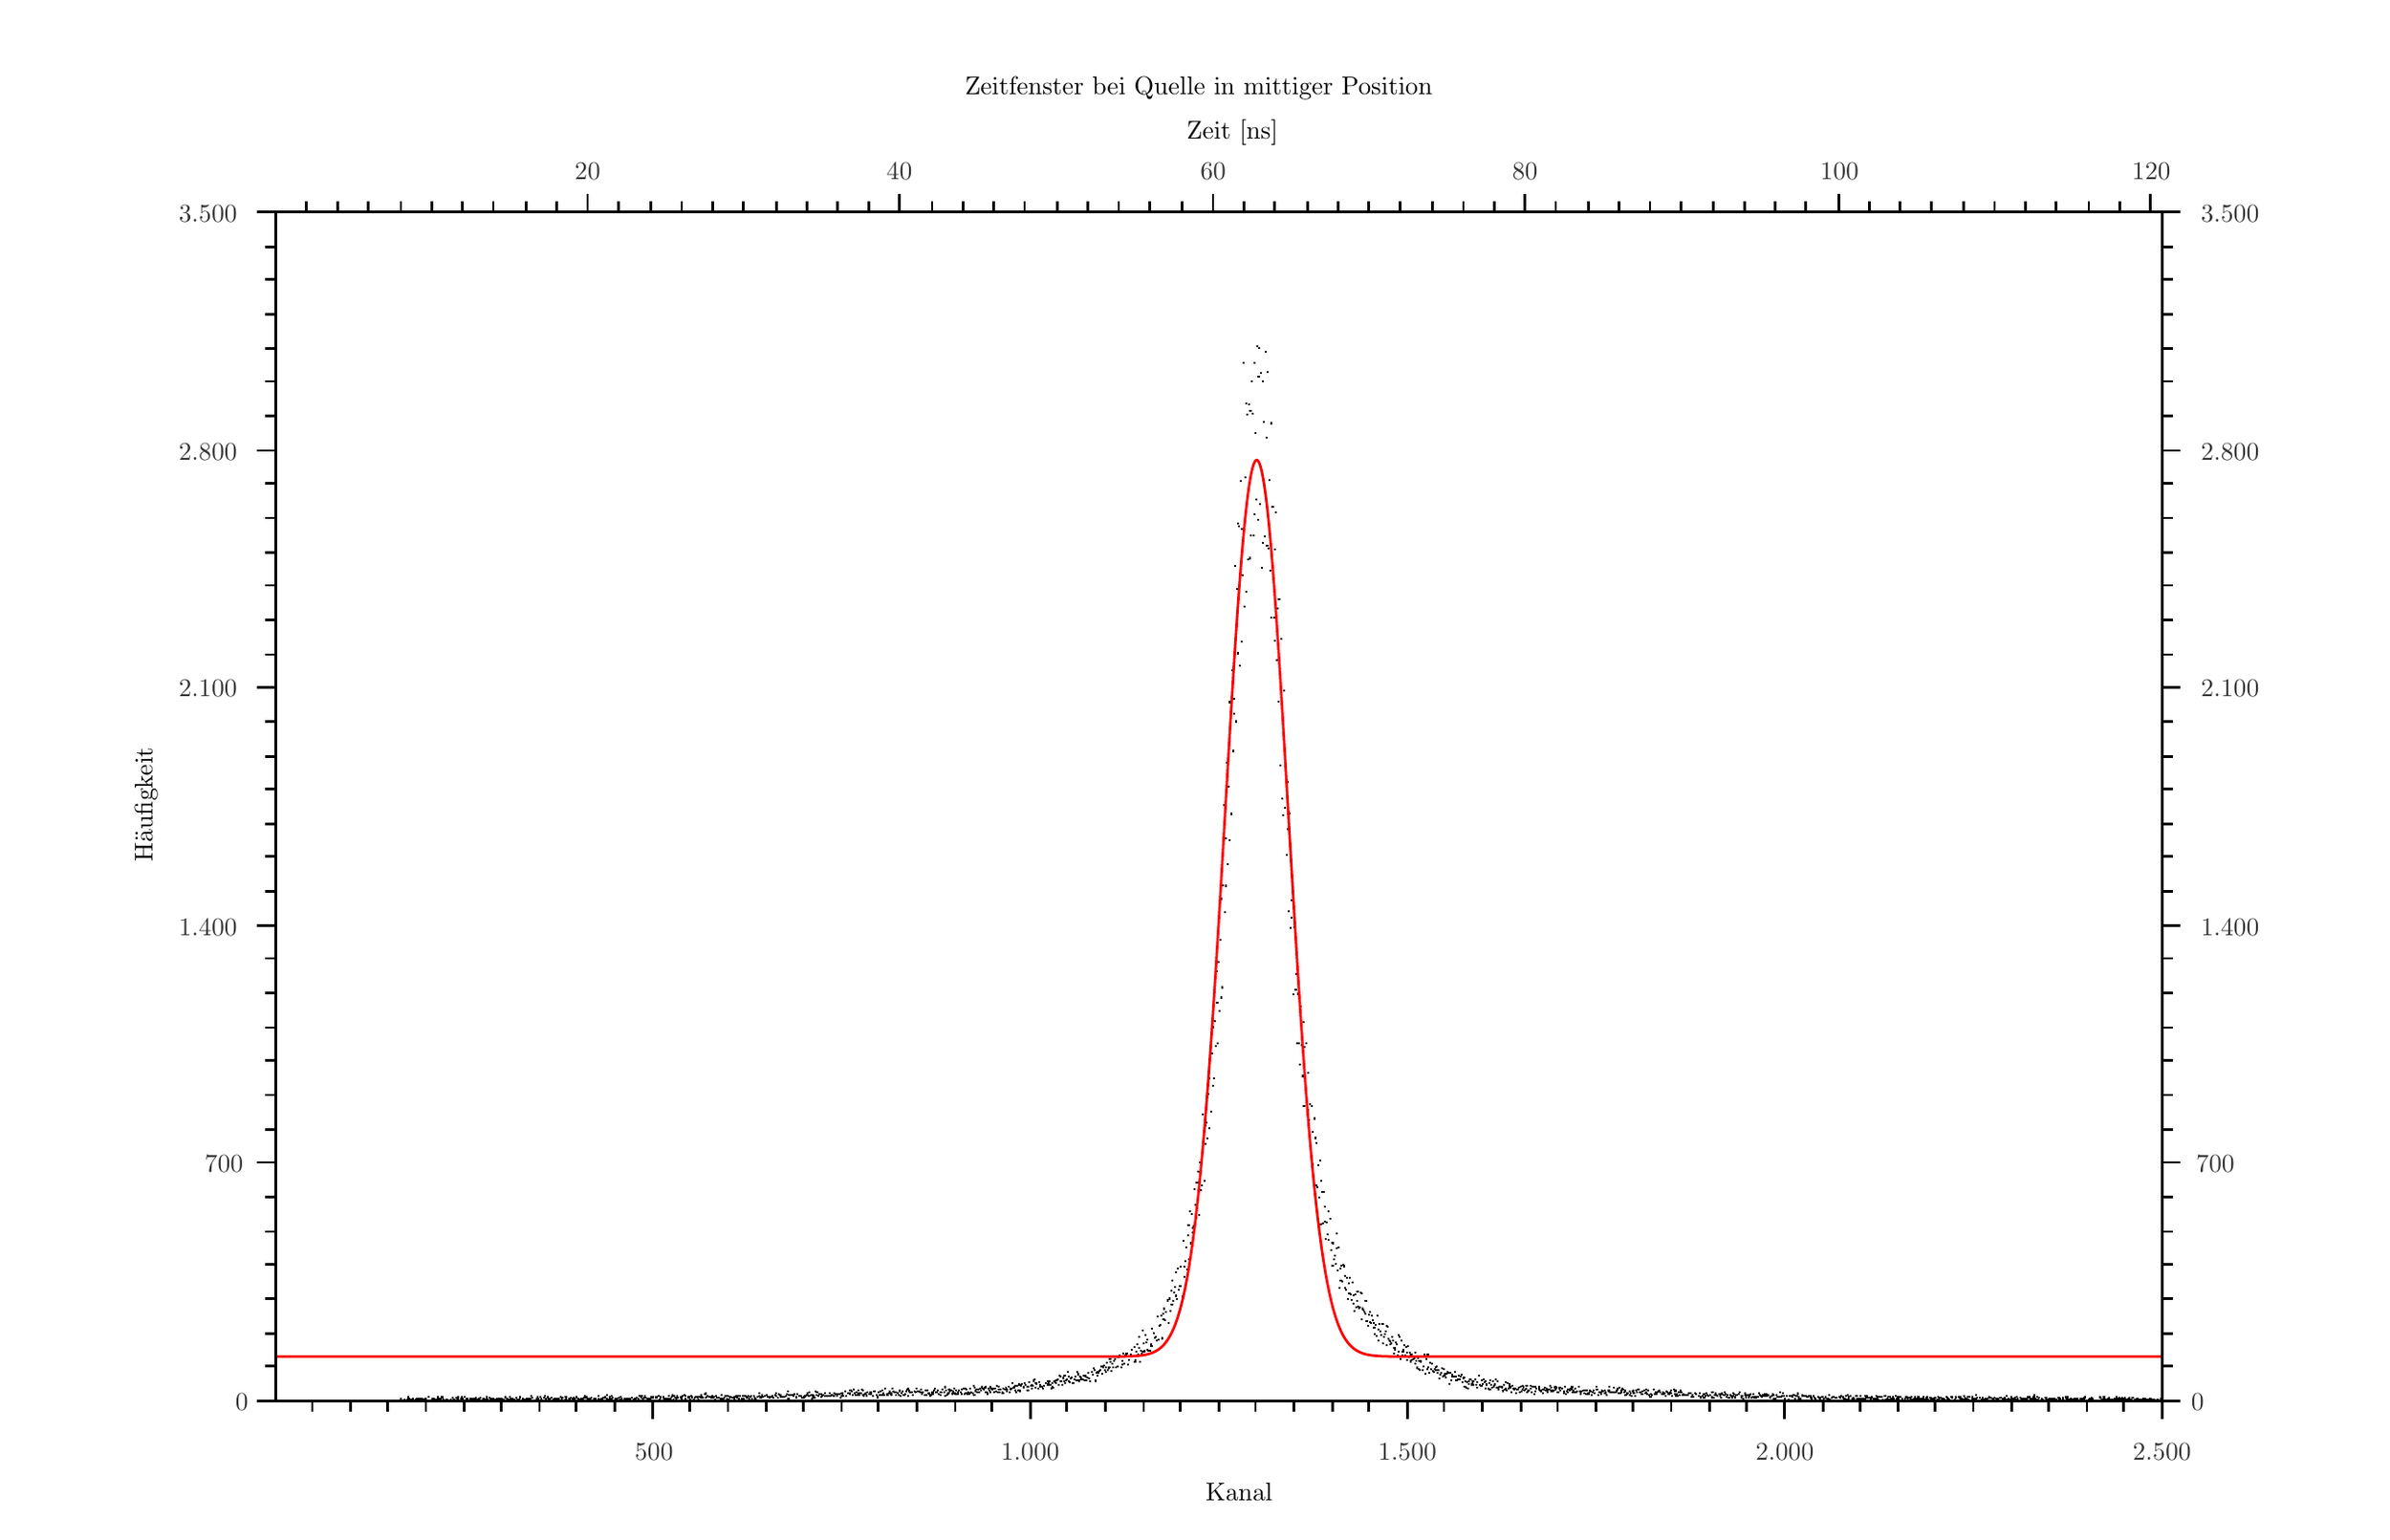
\begin{tikzpicture}{0pt}{0pt}{1215pt}{774pt}
	\clip(0pt,774pt) -- (914.667pt,774pt) -- (914.667pt,191.323pt) -- (0pt,191.323pt) -- (0pt,774pt);
\begin{scope}
	\clip(97.8656pt,700.977pt) -- (835.622pt,700.977pt) -- (835.622pt,235.739pt) -- (97.8656pt,235.739pt) -- (97.8656pt,700.977pt);
	\color[rgb]{0,0,0}
	\fill (145.987pt,236.138pt) rectangle (146.739pt,235.385pt);
	\color[rgb]{0,0,0}
	\fill (146.282pt,236.935pt) rectangle (147.035pt,236.183pt);
	\fill (146.577pt,236.271pt) rectangle (147.33pt,235.518pt);
	\fill (147.463pt,236.138pt) rectangle (148.215pt,235.385pt);
	\fill (148.053pt,236.537pt) rectangle (148.806pt,235.784pt);
	\fill (148.939pt,236.537pt) rectangle (149.692pt,235.784pt);
	\fill (149.234pt,237.6pt) rectangle (149.987pt,236.847pt);
	\fill (149.529pt,236.935pt) rectangle (150.282pt,236.183pt);
	\fill (149.824pt,236.67pt) rectangle (150.577pt,235.917pt);
	\fill (150.415pt,236.404pt) rectangle (151.168pt,235.651pt);
	\fill (151.005pt,236.802pt) rectangle (151.758pt,236.05pt);
	\fill (152.186pt,236.537pt) rectangle (152.939pt,235.784pt);
	\fill (152.481pt,236.138pt) rectangle (153.234pt,235.385pt);
	\fill (152.777pt,236.935pt) rectangle (153.529pt,236.183pt);
	\fill (153.367pt,237.068pt) rectangle (154.12pt,236.316pt);
	\fill (153.662pt,236.138pt) rectangle (154.415pt,235.385pt);
	\fill (153.958pt,237.068pt) rectangle (154.71pt,236.316pt);
	\fill (154.253pt,236.67pt) rectangle (155.006pt,235.917pt);
	\fill (154.843pt,236.935pt) rectangle (155.596pt,236.183pt);
	\fill (155.138pt,236.537pt) rectangle (155.891pt,235.784pt);
	\fill (155.729pt,236.935pt) rectangle (156.482pt,236.183pt);
	\fill (156.319pt,237.068pt) rectangle (157.072pt,236.316pt);
	\fill (156.615pt,236.271pt) rectangle (157.367pt,235.518pt);
	\fill (157.205pt,237.6pt) rectangle (157.958pt,236.847pt);
	\fill (157.795pt,236.138pt) rectangle (158.548pt,235.385pt);
	\fill (158.681pt,237.068pt) rectangle (159.434pt,236.316pt);
	\fill (158.976pt,236.67pt) rectangle (159.729pt,235.917pt);
	\fill (159.272pt,237.068pt) rectangle (160.024pt,236.316pt);
	\fill (159.567pt,236.802pt) rectangle (160.32pt,236.05pt);
	\fill (160.157pt,236.537pt) rectangle (160.91pt,235.784pt);
	\fill (160.748pt,237.6pt) rectangle (161.5pt,236.847pt);
	\fill (161.043pt,236.802pt) rectangle (161.796pt,236.05pt);
	\fill (161.633pt,236.935pt) rectangle (162.386pt,236.183pt);
	\fill (161.928pt,236.67pt) rectangle (162.681pt,235.917pt);
	\fill (162.519pt,237.467pt) rectangle (163.272pt,236.714pt);
	\fill (163.109pt,236.67pt) rectangle (163.862pt,235.917pt);
	\fill (163.995pt,236.537pt) rectangle (164.748pt,235.784pt);
	\fill (164.585pt,236.537pt) rectangle (165.338pt,235.784pt);
	\fill (165.471pt,236.271pt) rectangle (166.224pt,235.518pt);
	\fill (166.062pt,236.404pt) rectangle (166.814pt,235.651pt);
	\fill (166.652pt,237.201pt) rectangle (167.405pt,236.448pt);
	\fill (166.947pt,236.67pt) rectangle (167.7pt,235.917pt);
	\fill (167.538pt,236.67pt) rectangle (168.29pt,235.917pt);
	\fill (168.128pt,237.334pt) rectangle (168.881pt,236.581pt);
	\fill (168.423pt,236.404pt) rectangle (169.176pt,235.651pt);
	\fill (168.719pt,237.6pt) rectangle (169.471pt,236.847pt);
	\fill (169.014pt,237.068pt) rectangle (169.767pt,236.316pt);
	\fill (169.899pt,236.802pt) rectangle (170.652pt,236.05pt);
	\fill (170.195pt,237.467pt) rectangle (170.947pt,236.714pt);
	\fill (170.785pt,237.068pt) rectangle (171.538pt,236.316pt);
	\fill (171.376pt,237.6pt) rectangle (172.128pt,236.847pt);
	\fill (172.261pt,236.802pt) rectangle (173.014pt,236.05pt);
	\fill (172.556pt,236.935pt) rectangle (173.309pt,236.183pt);
	\fill (172.852pt,236.138pt) rectangle (173.604pt,235.385pt);
	\fill (173.737pt,237.068pt) rectangle (174.49pt,236.316pt);
	\fill (174.328pt,236.537pt) rectangle (175.081pt,235.784pt);
	\fill (174.623pt,237.068pt) rectangle (175.376pt,236.316pt);
	\fill (175.213pt,236.802pt) rectangle (175.966pt,236.05pt);
	\fill (175.804pt,237.334pt) rectangle (176.557pt,236.581pt);
	\fill (176.099pt,236.404pt) rectangle (176.852pt,235.651pt);
	\fill (176.69pt,236.802pt) rectangle (177.442pt,236.05pt);
	\fill (176.985pt,237.068pt) rectangle (177.738pt,236.316pt);
	\fill (177.575pt,237.334pt) rectangle (178.328pt,236.581pt);
	\fill (178.166pt,236.271pt) rectangle (178.918pt,235.518pt);
	\fill (178.461pt,237.068pt) rectangle (179.214pt,236.316pt);
	\fill (179.051pt,237.068pt) rectangle (179.804pt,236.316pt);
	\fill (179.642pt,236.404pt) rectangle (180.395pt,235.651pt);
	\fill (179.937pt,237.467pt) rectangle (180.69pt,236.714pt);
	\fill (180.527pt,236.537pt) rectangle (181.28pt,235.784pt);
	\fill (181.118pt,237.201pt) rectangle (181.871pt,236.448pt);
	\fill (181.413pt,236.67pt) rectangle (182.166pt,235.917pt);
	\fill (182.003pt,237.068pt) rectangle (182.756pt,236.316pt);
	\fill (182.299pt,236.67pt) rectangle (183.052pt,235.917pt);
	\fill (182.594pt,236.935pt) rectangle (183.347pt,236.183pt);
	\fill (183.48pt,236.67pt) rectangle (184.232pt,235.917pt);
	\fill (184.07pt,236.935pt) rectangle (184.823pt,236.183pt);
	\fill (184.365pt,236.802pt) rectangle (185.118pt,236.05pt);
	\fill (184.956pt,236.935pt) rectangle (185.709pt,236.183pt);
	\fill (185.841pt,236.935pt) rectangle (186.594pt,236.183pt);
	\fill (186.137pt,236.537pt) rectangle (186.889pt,235.784pt);
	\fill (186.432pt,236.404pt) rectangle (187.185pt,235.651pt);
	\fill (187.317pt,237.467pt) rectangle (188.07pt,236.714pt);
	\fill (187.908pt,237.068pt) rectangle (188.661pt,236.316pt);
	\fill (188.794pt,236.404pt) rectangle (189.546pt,235.651pt);
	\fill (189.089pt,237.6pt) rectangle (189.842pt,236.847pt);
	\fill (189.384pt,237.068pt) rectangle (190.137pt,236.316pt);
	\fill (189.679pt,236.271pt) rectangle (190.432pt,235.518pt);
	\fill (190.27pt,236.802pt) rectangle (191.022pt,236.05pt);
	\fill (190.86pt,236.537pt) rectangle (191.613pt,235.784pt);
	\fill (191.746pt,237.334pt) rectangle (192.499pt,236.581pt);
	\fill (192.041pt,236.67pt) rectangle (192.794pt,235.917pt);
	\fill (192.631pt,236.404pt) rectangle (193.384pt,235.651pt);
	\fill (192.927pt,237.201pt) rectangle (193.679pt,236.448pt);
	\fill (193.222pt,237.467pt) rectangle (193.975pt,236.714pt);
	\fill (194.108pt,236.802pt) rectangle (194.86pt,236.05pt);
	\fill (194.698pt,236.67pt) rectangle (195.451pt,235.917pt);
	\fill (195.584pt,236.935pt) rectangle (196.336pt,236.183pt);
	\fill (196.174pt,236.935pt) rectangle (196.927pt,236.183pt);
	\fill (197.06pt,236.935pt) rectangle (197.813pt,236.183pt);
	\fill (197.355pt,237.866pt) rectangle (198.108pt,237.113pt);
	\fill (197.65pt,237.334pt) rectangle (198.403pt,236.581pt);
	\fill (198.536pt,236.271pt) rectangle (199.289pt,235.518pt);
	\fill (199.126pt,236.271pt) rectangle (199.879pt,235.518pt);
	\fill (199.422pt,236.935pt) rectangle (200.174pt,236.183pt);
	\fill (200.012pt,237.733pt) rectangle (200.765pt,236.98pt);
	\fill (200.307pt,237.068pt) rectangle (201.06pt,236.316pt);
	\fill (200.898pt,237.733pt) rectangle (201.65pt,236.98pt);
	\fill (201.488pt,237.068pt) rectangle (202.241pt,236.316pt);
	\fill (202.374pt,237.334pt) rectangle (203.127pt,236.581pt);
	\fill (202.964pt,237.999pt) rectangle (203.717pt,237.246pt);
	\fill (203.259pt,237.068pt) rectangle (204.012pt,236.316pt);
	\fill (203.85pt,237.467pt) rectangle (204.603pt,236.714pt);
	\fill (204.145pt,236.802pt) rectangle (204.898pt,236.05pt);
	\fill (204.44pt,236.67pt) rectangle (205.193pt,235.917pt);
	\fill (204.735pt,237.068pt) rectangle (205.488pt,236.316pt);
	\fill (205.326pt,237.201pt) rectangle (206.079pt,236.448pt);
	\fill (205.916pt,236.404pt) rectangle (206.669pt,235.651pt);
	\fill (206.507pt,237.068pt) rectangle (207.26pt,236.316pt);
	\fill (206.802pt,236.537pt) rectangle (207.555pt,235.784pt);
	\fill (207.097pt,237.068pt) rectangle (207.85pt,236.316pt);
	\fill (207.688pt,236.935pt) rectangle (208.44pt,236.183pt);
	\fill (208.278pt,236.802pt) rectangle (209.031pt,236.05pt);
	\fill (208.869pt,237.6pt) rectangle (209.621pt,236.847pt);
	\fill (209.164pt,237.201pt) rectangle (209.917pt,236.448pt);
	\fill (209.459pt,236.67pt) rectangle (210.212pt,235.917pt);
	\fill (209.754pt,237.334pt) rectangle (210.507pt,236.581pt);
	\fill (210.64pt,236.404pt) rectangle (211.393pt,235.651pt);
	\fill (210.935pt,237.6pt) rectangle (211.688pt,236.847pt);
	\fill (211.23pt,236.935pt) rectangle (211.983pt,236.183pt);
	\fill (212.116pt,237.068pt) rectangle (212.869pt,236.316pt);
	\fill (212.706pt,236.802pt) rectangle (213.459pt,236.05pt);
	\fill (213.002pt,237.201pt) rectangle (213.754pt,236.448pt);
	\fill (213.592pt,236.802pt) rectangle (214.345pt,236.05pt);
	\fill (214.183pt,237.334pt) rectangle (214.935pt,236.581pt);
	\fill (214.478pt,236.802pt) rectangle (215.231pt,236.05pt);
	\fill (215.068pt,237.467pt) rectangle (215.821pt,236.714pt);
	\fill (215.954pt,236.802pt) rectangle (216.707pt,236.05pt);
	\fill (216.544pt,236.537pt) rectangle (217.297pt,235.784pt);
	\fill (216.84pt,237.068pt) rectangle (217.592pt,236.316pt);
	\fill (217.43pt,236.935pt) rectangle (218.183pt,236.183pt);
	\fill (217.725pt,236.67pt) rectangle (218.478pt,235.917pt);
	\fill (218.02pt,237.334pt) rectangle (218.773pt,236.581pt);
	\fill (218.316pt,237.866pt) rectangle (219.068pt,237.113pt);
	\fill (218.906pt,237.467pt) rectangle (219.659pt,236.714pt);
	\fill (219.497pt,237.068pt) rectangle (220.249pt,236.316pt);
	\fill (220.087pt,236.802pt) rectangle (220.84pt,236.05pt);
	\fill (220.382pt,236.67pt) rectangle (221.135pt,235.917pt);
	\fill (220.973pt,237.201pt) rectangle (221.725pt,236.448pt);
	\fill (221.858pt,236.935pt) rectangle (222.611pt,236.183pt);
	\fill (222.153pt,236.802pt) rectangle (222.906pt,236.05pt);
	\fill (222.744pt,236.802pt) rectangle (223.497pt,236.05pt);
	\fill (223.334pt,236.138pt) rectangle (224.087pt,235.385pt);
	\fill (223.63pt,237.999pt) rectangle (224.382pt,237.246pt);
	\fill (223.925pt,236.935pt) rectangle (224.678pt,236.183pt);
	\fill (224.22pt,236.67pt) rectangle (224.973pt,235.917pt);
	\fill (224.81pt,237.068pt) rectangle (225.563pt,236.316pt);
	\fill (225.106pt,236.537pt) rectangle (225.859pt,235.784pt);
	\fill (225.696pt,237.201pt) rectangle (226.449pt,236.448pt);
	\fill (226.287pt,237.467pt) rectangle (227.039pt,236.714pt);
	\fill (226.877pt,238.265pt) rectangle (227.63pt,237.512pt);
	\fill (227.172pt,237.068pt) rectangle (227.925pt,236.316pt);
	\fill (227.763pt,236.67pt) rectangle (228.515pt,235.917pt);
	\fill (228.058pt,237.467pt) rectangle (228.811pt,236.714pt);
	\fill (228.648pt,237.068pt) rectangle (229.401pt,236.316pt);
	\fill (228.944pt,238.132pt) rectangle (229.696pt,237.379pt);
	\fill (229.239pt,237.201pt) rectangle (229.992pt,236.448pt);
	\fill (230.124pt,237.068pt) rectangle (230.877pt,236.316pt);
	\fill (231.01pt,237.068pt) rectangle (231.763pt,236.316pt);
	\fill (231.601pt,237.334pt) rectangle (232.353pt,236.581pt);
	\fill (232.191pt,236.67pt) rectangle (232.944pt,235.917pt);
	\fill (232.486pt,237.733pt) rectangle (233.239pt,236.98pt);
	\fill (232.781pt,236.935pt) rectangle (233.534pt,236.183pt);
	\fill (233.077pt,236.271pt) rectangle (233.829pt,235.518pt);
	\fill (233.962pt,237.068pt) rectangle (234.715pt,236.316pt);
	\fill (234.553pt,236.935pt) rectangle (235.306pt,236.183pt);
	\fill (235.438pt,236.935pt) rectangle (236.191pt,236.183pt);
	\fill (235.734pt,236.271pt) rectangle (236.486pt,235.518pt);
	\fill (236.029pt,236.935pt) rectangle (236.782pt,236.183pt);
	\fill (236.324pt,236.138pt) rectangle (237.077pt,235.385pt);
	\fill (236.915pt,237.334pt) rectangle (237.667pt,236.581pt);
	\fill (237.505pt,236.537pt) rectangle (238.258pt,235.784pt);
	\fill (237.8pt,236.802pt) rectangle (238.553pt,236.05pt);
	\fill (238.095pt,236.935pt) rectangle (238.848pt,236.183pt);
	\fill (238.391pt,236.802pt) rectangle (239.143pt,236.05pt);
	\fill (238.686pt,237.334pt) rectangle (239.439pt,236.581pt);
	\fill (239.276pt,236.935pt) rectangle (240.029pt,236.183pt);
	\fill (239.867pt,237.999pt) rectangle (240.62pt,237.246pt);
	\fill (240.457pt,237.201pt) rectangle (241.21pt,236.448pt);
	\fill (240.752pt,237.866pt) rectangle (241.505pt,237.113pt);
	\fill (241.048pt,237.068pt) rectangle (241.8pt,236.316pt);
	\fill (241.343pt,237.201pt) rectangle (242.096pt,236.448pt);
	\fill (241.933pt,237.866pt) rectangle (242.686pt,237.113pt);
	\fill (242.228pt,237.201pt) rectangle (242.981pt,236.448pt);
	\fill (242.819pt,236.935pt) rectangle (243.572pt,236.183pt);
	\fill (243.409pt,236.802pt) rectangle (244.162pt,236.05pt);
	\fill (243.705pt,237.068pt) rectangle (244.457pt,236.316pt);
	\fill (244pt,236.67pt) rectangle (244.753pt,235.917pt);
	\fill (244.295pt,237.467pt) rectangle (245.048pt,236.714pt);
	\fill (245.181pt,237.467pt) rectangle (245.934pt,236.714pt);
	\fill (246.066pt,237.334pt) rectangle (246.819pt,236.581pt);
	\fill (246.362pt,237.733pt) rectangle (247.114pt,236.98pt);
	\fill (246.657pt,237.201pt) rectangle (247.41pt,236.448pt);
	\fill (247.247pt,238.132pt) rectangle (248pt,237.379pt);
	\fill (247.542pt,236.537pt) rectangle (248.295pt,235.784pt);
	\fill (248.133pt,237.467pt) rectangle (248.886pt,236.714pt);
	\fill (249.019pt,237.467pt) rectangle (249.771pt,236.714pt);
	\fill (249.314pt,236.67pt) rectangle (250.067pt,235.917pt);
	\fill (249.609pt,237.068pt) rectangle (250.362pt,236.316pt);
	\fill (250.199pt,236.802pt) rectangle (250.952pt,236.05pt);
	\fill (250.495pt,236.935pt) rectangle (251.247pt,236.183pt);
	\fill (251.085pt,236.935pt) rectangle (251.838pt,236.183pt);
	\fill (251.38pt,237.999pt) rectangle (252.133pt,237.246pt);
	\fill (251.971pt,236.802pt) rectangle (252.724pt,236.05pt);
	\fill (252.266pt,237.6pt) rectangle (253.019pt,236.847pt);
	\fill (252.561pt,238.265pt) rectangle (253.314pt,237.512pt);
	\fill (252.856pt,237.999pt) rectangle (253.609pt,237.246pt);
	\fill (253.152pt,236.404pt) rectangle (253.904pt,235.651pt);
	\fill (253.447pt,237.866pt) rectangle (254.2pt,237.113pt);
	\fill (253.742pt,237.201pt) rectangle (254.495pt,236.448pt);
	\fill (254.037pt,236.802pt) rectangle (254.79pt,236.05pt);
	\fill (254.333pt,237.866pt) rectangle (255.085pt,237.113pt);
	\fill (254.628pt,237.6pt) rectangle (255.381pt,236.847pt);
	\fill (254.923pt,237.334pt) rectangle (255.676pt,236.581pt);
	\fill (255.809pt,237.467pt) rectangle (256.561pt,236.714pt);
	\fill (256.104pt,237.733pt) rectangle (256.857pt,236.98pt);
	\fill (256.399pt,237.068pt) rectangle (257.152pt,236.316pt);
	\fill (256.694pt,237.866pt) rectangle (257.447pt,237.113pt);
	\fill (257.285pt,238.53pt) rectangle (258.038pt,237.778pt);
	\fill (257.58pt,237.999pt) rectangle (258.333pt,237.246pt);
	\fill (257.875pt,236.935pt) rectangle (258.628pt,236.183pt);
	\fill (258.761pt,237.467pt) rectangle (259.514pt,236.714pt);
	\fill (259.351pt,237.467pt) rectangle (260.104pt,236.714pt);
	\fill (259.647pt,236.404pt) rectangle (260.399pt,235.651pt);
	\fill (259.942pt,237.866pt) rectangle (260.695pt,237.113pt);
	\fill (260.237pt,237.467pt) rectangle (260.99pt,236.714pt);
	\fill (261.123pt,236.537pt) rectangle (261.875pt,235.784pt);
	\fill (261.418pt,237.334pt) rectangle (262.171pt,236.581pt);
	\fill (261.713pt,237.6pt) rectangle (262.466pt,236.847pt);
	\fill (262.303pt,237.733pt) rectangle (263.056pt,236.98pt);
	\fill (262.599pt,237.467pt) rectangle (263.352pt,236.714pt);
	\fill (262.894pt,236.67pt) rectangle (263.647pt,235.917pt);
	\fill (263.189pt,237.6pt) rectangle (263.942pt,236.847pt);
	\fill (263.78pt,238.265pt) rectangle (264.532pt,237.512pt);
	\fill (264.075pt,237.467pt) rectangle (264.828pt,236.714pt);
	\fill (264.665pt,237.334pt) rectangle (265.418pt,236.581pt);
	\fill (265.256pt,238.663pt) rectangle (266.009pt,237.911pt);
	\fill (265.551pt,237.334pt) rectangle (266.304pt,236.581pt);
	\fill (265.846pt,238.929pt) rectangle (266.599pt,238.176pt);
	\fill (266.141pt,237.6pt) rectangle (266.894pt,236.847pt);
	\fill (266.437pt,237.999pt) rectangle (267.189pt,237.246pt);
	\fill (267.027pt,237.733pt) rectangle (267.78pt,236.98pt);
	\fill (267.322pt,237.6pt) rectangle (268.075pt,236.847pt);
	\fill (267.913pt,237.467pt) rectangle (268.665pt,236.714pt);
	\fill (268.208pt,237.999pt) rectangle (268.961pt,237.246pt);
	\fill (268.503pt,237.334pt) rectangle (269.256pt,236.581pt);
	\fill (269.094pt,237.733pt) rectangle (269.846pt,236.98pt);
	\fill (269.389pt,236.537pt) rectangle (270.142pt,235.784pt);
	\fill (269.684pt,237.866pt) rectangle (270.437pt,237.113pt);
	\fill (269.979pt,237.334pt) rectangle (270.732pt,236.581pt);
	\fill (270.865pt,237.201pt) rectangle (271.618pt,236.448pt);
	\fill (271.455pt,237.068pt) rectangle (272.208pt,236.316pt);
	\fill (271.751pt,238.265pt) rectangle (272.503pt,237.512pt);
	\fill (272.046pt,236.67pt) rectangle (272.799pt,235.917pt);
	\fill (272.341pt,237.068pt) rectangle (273.094pt,236.316pt);
	\fill (272.636pt,236.67pt) rectangle (273.389pt,235.917pt);
	\fill (272.931pt,237.334pt) rectangle (273.684pt,236.581pt);
	\fill (273.227pt,238.132pt) rectangle (273.979pt,237.379pt);
	\fill (273.817pt,238.132pt) rectangle (274.57pt,237.379pt);
	\fill (274.112pt,237.068pt) rectangle (274.865pt,236.316pt);
	\fill (274.408pt,237.999pt) rectangle (275.16pt,237.246pt);
	\fill (274.703pt,236.67pt) rectangle (275.456pt,235.917pt);
	\fill (274.998pt,237.467pt) rectangle (275.751pt,236.714pt);
	\fill (275.293pt,237.6pt) rectangle (276.046pt,236.847pt);
	\fill (275.588pt,237.733pt) rectangle (276.341pt,236.98pt);
	\fill (276.179pt,237.201pt) rectangle (276.932pt,236.448pt);
	\fill (276.769pt,236.802pt) rectangle (277.522pt,236.05pt);
	\fill (277.065pt,237.733pt) rectangle (277.817pt,236.98pt);
	\fill (277.655pt,237.866pt) rectangle (278.408pt,237.113pt);
	\fill (277.95pt,237.467pt) rectangle (278.703pt,236.714pt);
	\fill (278.245pt,238.132pt) rectangle (278.998pt,237.379pt);
	\fill (278.836pt,236.935pt) rectangle (279.589pt,236.183pt);
	\fill (279.131pt,238.132pt) rectangle (279.884pt,237.379pt);
	\fill (279.722pt,237.068pt) rectangle (280.474pt,236.316pt);
	\fill (280.312pt,238.132pt) rectangle (281.065pt,237.379pt);
	\fill (280.607pt,236.935pt) rectangle (281.36pt,236.183pt);
	\fill (281.198pt,237.866pt) rectangle (281.95pt,237.113pt);
	\fill (281.493pt,237.467pt) rectangle (282.246pt,236.714pt);
	\fill (282.083pt,237.201pt) rectangle (282.836pt,236.448pt);
	\fill (282.378pt,237.999pt) rectangle (283.131pt,237.246pt);
	\fill (282.674pt,236.802pt) rectangle (283.427pt,236.05pt);
	\fill (282.969pt,237.6pt) rectangle (283.722pt,236.847pt);
	\fill (283.559pt,237.999pt) rectangle (284.312pt,237.246pt);
	\fill (283.855pt,237.068pt) rectangle (284.607pt,236.316pt);
	\fill (284.445pt,237.999pt) rectangle (285.198pt,237.246pt);
	\fill (284.74pt,237.201pt) rectangle (285.493pt,236.448pt);
	\fill (285.035pt,237.068pt) rectangle (285.788pt,236.316pt);
	\fill (285.921pt,237.6pt) rectangle (286.674pt,236.847pt);
	\fill (286.512pt,237.999pt) rectangle (287.264pt,237.246pt);
	\fill (286.807pt,239.062pt) rectangle (287.56pt,238.309pt);
	\fill (287.102pt,237.201pt) rectangle (287.855pt,236.448pt);
	\fill (287.397pt,237.467pt) rectangle (288.15pt,236.714pt);
	\fill (287.692pt,238.265pt) rectangle (288.445pt,237.512pt);
	\fill (287.988pt,237.733pt) rectangle (288.74pt,236.98pt);
	\fill (288.873pt,237.866pt) rectangle (289.626pt,237.113pt);
	\fill (289.464pt,238.265pt) rectangle (290.217pt,237.512pt);
	\fill (289.759pt,237.6pt) rectangle (290.512pt,236.847pt);
	\fill (290.349pt,237.733pt) rectangle (291.102pt,236.98pt);
	\fill (290.645pt,237.467pt) rectangle (291.397pt,236.714pt);
	\fill (291.235pt,237.733pt) rectangle (291.988pt,236.98pt);
	\fill (291.826pt,238.132pt) rectangle (292.578pt,237.379pt);
	\fill (292.121pt,237.334pt) rectangle (292.874pt,236.581pt);
	\fill (292.711pt,238.398pt) rectangle (293.464pt,237.645pt);
	\fill (293.006pt,237.866pt) rectangle (293.759pt,237.113pt);
	\fill (293.302pt,239.062pt) rectangle (294.054pt,238.309pt);
	\fill (293.892pt,237.201pt) rectangle (294.645pt,236.448pt);
	\fill (294.187pt,238.663pt) rectangle (294.94pt,237.911pt);
	\fill (294.483pt,238.265pt) rectangle (295.235pt,237.512pt);
	\fill (294.778pt,238.398pt) rectangle (295.531pt,237.645pt);
	\fill (295.073pt,237.733pt) rectangle (295.826pt,236.98pt);
	\fill (295.663pt,237.733pt) rectangle (296.416pt,236.98pt);
	\fill (295.959pt,237.6pt) rectangle (296.711pt,236.847pt);
	\fill (296.254pt,237.733pt) rectangle (297.007pt,236.98pt);
	\fill (296.549pt,237.6pt) rectangle (297.302pt,236.847pt);
	\fill (297.14pt,237.999pt) rectangle (297.892pt,237.246pt);
	\fill (297.435pt,238.663pt) rectangle (298.188pt,237.911pt);
	\fill (297.73pt,239.86pt) rectangle (298.483pt,239.107pt);
	\fill (298.025pt,237.068pt) rectangle (298.778pt,236.316pt);
	\fill (298.32pt,238.53pt) rectangle (299.073pt,237.778pt);
	\fill (298.616pt,238.265pt) rectangle (299.368pt,237.512pt);
	\fill (298.911pt,238.398pt) rectangle (299.664pt,237.645pt);
	\fill (299.501pt,238.53pt) rectangle (300.254pt,237.778pt);
	\fill (300.092pt,238.132pt) rectangle (300.845pt,237.379pt);
	\fill (300.387pt,238.663pt) rectangle (301.14pt,237.911pt);
	\fill (300.977pt,237.467pt) rectangle (301.73pt,236.714pt);
	\fill (301.568pt,238.796pt) rectangle (302.321pt,238.044pt);
	\fill (302.158pt,237.866pt) rectangle (302.911pt,237.113pt);
	\fill (302.453pt,237.999pt) rectangle (303.206pt,237.246pt);
	\fill (303.044pt,237.999pt) rectangle (303.797pt,237.246pt);
	\fill (303.339pt,237.201pt) rectangle (304.092pt,236.448pt);
	\fill (303.93pt,237.467pt) rectangle (304.682pt,236.714pt);
	\fill (304.225pt,237.866pt) rectangle (304.978pt,237.113pt);
	\fill (304.52pt,237.6pt) rectangle (305.273pt,236.847pt);
	\fill (304.815pt,237.999pt) rectangle (305.568pt,237.246pt);
	\fill (305.11pt,238.398pt) rectangle (305.863pt,237.645pt);
	\fill (305.406pt,238.929pt) rectangle (306.159pt,238.176pt);
	\fill (305.996pt,237.999pt) rectangle (306.749pt,237.246pt);
	\fill (306.291pt,239.594pt) rectangle (307.044pt,238.841pt);
	\fill (306.882pt,238.398pt) rectangle (307.635pt,237.645pt);
	\fill (307.177pt,237.068pt) rectangle (307.93pt,236.316pt);
	\fill (307.472pt,238.265pt) rectangle (308.225pt,237.512pt);
	\fill (307.767pt,237.467pt) rectangle (308.52pt,236.714pt);
	\fill (308.063pt,237.866pt) rectangle (308.815pt,237.113pt);
	\fill (308.358pt,237.201pt) rectangle (309.111pt,236.448pt);
	\fill (308.653pt,239.727pt) rectangle (309.406pt,238.974pt);
	\fill (308.948pt,238.398pt) rectangle (309.701pt,237.645pt);
	\fill (309.244pt,239.461pt) rectangle (309.996pt,238.708pt);
	\fill (309.834pt,237.999pt) rectangle (310.587pt,237.246pt);
	\fill (310.129pt,238.663pt) rectangle (310.882pt,237.911pt);
	\fill (310.72pt,238.796pt) rectangle (311.472pt,238.044pt);
	\fill (311.015pt,237.6pt) rectangle (311.768pt,236.847pt);
	\fill (311.31pt,238.132pt) rectangle (312.063pt,237.379pt);
	\fill (311.605pt,238.53pt) rectangle (312.358pt,237.778pt);
	\fill (312.196pt,239.062pt) rectangle (312.949pt,238.309pt);
	\fill (312.491pt,237.999pt) rectangle (313.244pt,237.246pt);
	\fill (313.081pt,237.866pt) rectangle (313.834pt,237.113pt);
	\fill (313.672pt,238.132pt) rectangle (314.425pt,237.379pt);
	\fill (314.262pt,239.195pt) rectangle (315.015pt,238.442pt);
	\fill (314.558pt,237.866pt) rectangle (315.31pt,237.113pt);
	\fill (314.853pt,238.398pt) rectangle (315.606pt,237.645pt);
	\fill (315.148pt,238.398pt) rectangle (315.901pt,237.645pt);
	\fill (315.738pt,237.866pt) rectangle (316.491pt,237.113pt);
	\fill (316.034pt,239.195pt) rectangle (316.786pt,238.442pt);
	\fill (316.329pt,238.663pt) rectangle (317.082pt,237.911pt);
	\fill (316.624pt,238.796pt) rectangle (317.377pt,238.044pt);
	\fill (316.919pt,237.999pt) rectangle (317.672pt,237.246pt);
	\fill (317.51pt,238.663pt) rectangle (318.263pt,237.911pt);
	\fill (318.1pt,238.663pt) rectangle (318.853pt,237.911pt);
	\fill (318.395pt,237.201pt) rectangle (319.148pt,236.448pt);
	\fill (318.691pt,237.999pt) rectangle (319.443pt,237.246pt);
	\fill (318.986pt,239.195pt) rectangle (319.739pt,238.442pt);
	\fill (319.281pt,238.398pt) rectangle (320.034pt,237.645pt);
	\fill (319.576pt,237.999pt) rectangle (320.329pt,237.246pt);
	\fill (320.167pt,239.727pt) rectangle (320.92pt,238.974pt);
	\fill (320.462pt,237.866pt) rectangle (321.215pt,237.113pt);
	\fill (321.348pt,239.062pt) rectangle (322.1pt,238.309pt);
	\fill (321.938pt,238.929pt) rectangle (322.691pt,238.176pt);
	\fill (322.233pt,240.126pt) rectangle (322.986pt,239.373pt);
	\fill (322.824pt,239.727pt) rectangle (323.577pt,238.974pt);
	\fill (323.119pt,238.265pt) rectangle (323.872pt,237.512pt);
	\fill (323.414pt,240.391pt) rectangle (324.167pt,239.639pt);
	\fill (323.709pt,239.062pt) rectangle (324.462pt,238.309pt);
	\fill (324.3pt,238.53pt) rectangle (325.053pt,237.778pt);
	\fill (324.595pt,239.461pt) rectangle (325.348pt,238.708pt);
	\fill (324.89pt,238.398pt) rectangle (325.643pt,237.645pt);
	\fill (325.185pt,240.259pt) rectangle (325.938pt,239.506pt);
	\fill (325.481pt,239.195pt) rectangle (326.234pt,238.442pt);
	\fill (325.776pt,238.398pt) rectangle (326.529pt,237.645pt);
	\fill (326.366pt,239.195pt) rectangle (327.119pt,238.442pt);
	\fill (326.662pt,240.391pt) rectangle (327.414pt,239.639pt);
	\fill (326.957pt,238.53pt) rectangle (327.71pt,237.778pt);
	\fill (327.252pt,240.126pt) rectangle (328.005pt,239.373pt);
	\fill (327.547pt,237.999pt) rectangle (328.3pt,237.246pt);
	\fill (327.842pt,238.663pt) rectangle (328.595pt,237.911pt);
	\fill (328.138pt,238.929pt) rectangle (328.89pt,238.176pt);
	\fill (328.433pt,237.999pt) rectangle (329.186pt,237.246pt);
	\fill (328.728pt,238.53pt) rectangle (329.481pt,237.778pt);
	\fill (329.023pt,239.328pt) rectangle (329.776pt,238.575pt);
	\fill (329.614pt,238.663pt) rectangle (330.367pt,237.911pt);
	\fill (329.909pt,239.328pt) rectangle (330.662pt,238.575pt);
	\fill (330.204pt,239.594pt) rectangle (330.957pt,238.841pt);
	\fill (330.499pt,238.796pt) rectangle (331.252pt,238.044pt);
	\fill (331.09pt,238.132pt) rectangle (331.843pt,237.379pt);
	\fill (331.385pt,239.727pt) rectangle (332.138pt,238.974pt);
	\fill (331.68pt,239.727pt) rectangle (332.433pt,238.974pt);
	\fill (332.566pt,238.398pt) rectangle (333.319pt,237.645pt);
	\fill (332.861pt,237.467pt) rectangle (333.614pt,236.714pt);
	\fill (333.156pt,239.328pt) rectangle (333.909pt,238.575pt);
	\fill (333.747pt,238.398pt) rectangle (334.5pt,237.645pt);
	\fill (334.042pt,239.86pt) rectangle (334.795pt,239.107pt);
	\fill (334.337pt,238.265pt) rectangle (335.09pt,237.512pt);
	\fill (334.633pt,240.126pt) rectangle (335.385pt,239.373pt);
	\fill (334.928pt,238.398pt) rectangle (335.681pt,237.645pt);
	\fill (335.223pt,239.195pt) rectangle (335.976pt,238.442pt);
	\fill (335.518pt,238.53pt) rectangle (336.271pt,237.778pt);
	\fill (335.813pt,240.79pt) rectangle (336.566pt,240.037pt);
	\fill (336.404pt,238.663pt) rectangle (337.157pt,237.911pt);
	\fill (336.699pt,238.265pt) rectangle (337.452pt,237.512pt);
	\fill (336.994pt,238.265pt) rectangle (337.747pt,237.512pt);
	\fill (337.29pt,239.062pt) rectangle (338.042pt,238.309pt);
	\fill (337.585pt,239.727pt) rectangle (338.338pt,238.974pt);
	\fill (337.88pt,238.929pt) rectangle (338.633pt,238.176pt);
	\fill (338.175pt,238.265pt) rectangle (338.928pt,237.512pt);
	\fill (338.47pt,239.062pt) rectangle (339.223pt,238.309pt);
	\fill (338.766pt,240.923pt) rectangle (339.518pt,240.17pt);
	\fill (339.061pt,239.727pt) rectangle (339.814pt,238.974pt);
	\fill (339.356pt,239.328pt) rectangle (340.109pt,238.575pt);
	\fill (339.947pt,239.461pt) rectangle (340.699pt,238.708pt);
	\fill (340.242pt,238.398pt) rectangle (340.995pt,237.645pt);
	\fill (340.832pt,239.195pt) rectangle (341.585pt,238.442pt);
	\fill (341.127pt,238.53pt) rectangle (341.88pt,237.778pt);
	\fill (341.423pt,239.993pt) rectangle (342.175pt,239.24pt);
	\fill (342.013pt,237.866pt) rectangle (342.766pt,237.113pt);
	\fill (342.308pt,239.062pt) rectangle (343.061pt,238.309pt);
	\fill (342.603pt,239.86pt) rectangle (343.356pt,239.107pt);
	\fill (343.194pt,238.265pt) rectangle (343.947pt,237.512pt);
	\fill (343.784pt,238.796pt) rectangle (344.537pt,238.044pt);
	\fill (344.08pt,239.727pt) rectangle (344.832pt,238.974pt);
	\fill (344.375pt,240.524pt) rectangle (345.128pt,239.772pt);
	\fill (344.67pt,240.79pt) rectangle (345.423pt,240.037pt);
	\fill (344.965pt,237.999pt) rectangle (345.718pt,237.246pt);
	\fill (345.26pt,239.993pt) rectangle (346.013pt,239.24pt);
	\fill (345.556pt,239.328pt) rectangle (346.309pt,238.575pt);
	\fill (346.146pt,239.461pt) rectangle (346.899pt,238.708pt);
	\fill (346.737pt,238.398pt) rectangle (347.489pt,237.645pt);
	\fill (347.327pt,239.86pt) rectangle (348.08pt,239.107pt);
	\fill (347.622pt,239.594pt) rectangle (348.375pt,238.841pt);
	\fill (348.213pt,240.79pt) rectangle (348.965pt,240.037pt);
	\fill (348.508pt,239.86pt) rectangle (349.261pt,239.107pt);
	\fill (349.098pt,239.727pt) rectangle (349.851pt,238.974pt);
	\fill (349.689pt,239.461pt) rectangle (350.442pt,238.708pt);
	\fill (349.984pt,240.657pt) rectangle (350.737pt,239.904pt);
	\fill (350.279pt,238.796pt) rectangle (351.032pt,238.044pt);
	\fill (350.574pt,239.594pt) rectangle (351.327pt,238.841pt);
	\fill (351.46pt,238.265pt) rectangle (352.213pt,237.512pt);
	\fill (351.755pt,240.126pt) rectangle (352.508pt,239.373pt);
	\fill (352.051pt,238.265pt) rectangle (352.803pt,237.512pt);
	\fill (352.346pt,240.259pt) rectangle (353.099pt,239.506pt);
	\fill (352.936pt,239.195pt) rectangle (353.689pt,238.442pt);
	\fill (353.231pt,238.929pt) rectangle (353.984pt,238.176pt);
	\fill (353.527pt,238.132pt) rectangle (354.279pt,237.379pt);
	\fill (353.822pt,238.53pt) rectangle (354.575pt,237.778pt);
	\fill (354.117pt,239.328pt) rectangle (354.87pt,238.575pt);
	\fill (354.412pt,238.663pt) rectangle (355.165pt,237.911pt);
	\fill (354.708pt,239.461pt) rectangle (355.46pt,238.708pt);
	\fill (355.003pt,240.126pt) rectangle (355.756pt,239.373pt);
	\fill (355.298pt,240.79pt) rectangle (356.051pt,240.037pt);
	\fill (355.593pt,239.328pt) rectangle (356.346pt,238.575pt);
	\fill (355.888pt,239.594pt) rectangle (356.641pt,238.841pt);
	\fill (356.479pt,240.259pt) rectangle (357.232pt,239.506pt);
	\fill (356.774pt,238.796pt) rectangle (357.527pt,238.044pt);
	\fill (357.365pt,238.53pt) rectangle (358.117pt,237.778pt);
	\fill (357.66pt,239.461pt) rectangle (358.413pt,238.708pt);
	\fill (358.25pt,240.524pt) rectangle (359.003pt,239.772pt);
	\fill (358.841pt,239.328pt) rectangle (359.593pt,238.575pt);
	\fill (359.136pt,241.455pt) rectangle (359.889pt,240.702pt);
	\fill (359.431pt,238.132pt) rectangle (360.184pt,237.379pt);
	\fill (359.726pt,240.259pt) rectangle (360.479pt,239.506pt);
	\fill (360.022pt,238.398pt) rectangle (360.774pt,237.645pt);
	\fill (360.317pt,238.929pt) rectangle (361.07pt,238.176pt);
	\fill (360.612pt,239.195pt) rectangle (361.365pt,238.442pt);
	\fill (360.907pt,240.391pt) rectangle (361.66pt,239.639pt);
	\fill (361.202pt,239.993pt) rectangle (361.955pt,239.24pt);
	\fill (361.793pt,240.259pt) rectangle (362.546pt,239.506pt);
	\fill (362.088pt,238.929pt) rectangle (362.841pt,238.176pt);
	\fill (362.383pt,239.86pt) rectangle (363.136pt,239.107pt);
	\fill (362.678pt,239.195pt) rectangle (363.431pt,238.442pt);
	\fill (362.974pt,240.79pt) rectangle (363.727pt,240.037pt);
	\fill (363.269pt,238.929pt) rectangle (364.022pt,238.176pt);
	\fill (363.564pt,240.126pt) rectangle (364.317pt,239.373pt);
	\fill (364.155pt,238.663pt) rectangle (364.907pt,237.911pt);
	\fill (364.45pt,239.328pt) rectangle (365.203pt,238.575pt);
	\fill (364.745pt,240.126pt) rectangle (365.498pt,239.373pt);
	\fill (365.335pt,239.461pt) rectangle (366.088pt,238.708pt);
	\fill (365.631pt,240.657pt) rectangle (366.384pt,239.904pt);
	\fill (365.926pt,238.796pt) rectangle (366.679pt,238.044pt);
	\fill (366.516pt,241.056pt) rectangle (367.269pt,240.303pt);
	\fill (366.812pt,238.796pt) rectangle (367.564pt,238.044pt);
	\fill (367.107pt,240.79pt) rectangle (367.86pt,240.037pt);
	\fill (367.402pt,239.062pt) rectangle (368.155pt,238.309pt);
	\fill (367.697pt,240.391pt) rectangle (368.45pt,239.639pt);
	\fill (367.992pt,238.796pt) rectangle (368.745pt,238.044pt);
	\fill (368.288pt,239.328pt) rectangle (369.04pt,238.575pt);
	\fill (368.583pt,238.663pt) rectangle (369.336pt,237.911pt);
	\fill (368.878pt,239.195pt) rectangle (369.631pt,238.442pt);
	\fill (369.173pt,240.923pt) rectangle (369.926pt,240.17pt);
	\fill (369.469pt,239.328pt) rectangle (370.221pt,238.575pt);
	\fill (370.059pt,239.195pt) rectangle (370.812pt,238.442pt);
	\fill (370.354pt,241.854pt) rectangle (371.107pt,241.101pt);
	\fill (370.649pt,238.398pt) rectangle (371.402pt,237.645pt);
	\fill (370.945pt,241.322pt) rectangle (371.697pt,240.569pt);
	\fill (371.24pt,239.993pt) rectangle (371.993pt,239.24pt);
	\fill (371.535pt,240.391pt) rectangle (372.288pt,239.639pt);
	\fill (371.83pt,239.594pt) rectangle (372.583pt,238.841pt);
	\fill (372.126pt,240.657pt) rectangle (372.878pt,239.904pt);
	\fill (372.421pt,240.391pt) rectangle (373.174pt,239.639pt);
	\fill (372.716pt,239.328pt) rectangle (373.469pt,238.575pt);
	\fill (373.011pt,241.056pt) rectangle (373.764pt,240.303pt);
	\fill (373.306pt,240.259pt) rectangle (374.059pt,239.506pt);
	\fill (373.602pt,241.322pt) rectangle (374.354pt,240.569pt);
	\fill (373.897pt,241.455pt) rectangle (374.65pt,240.702pt);
	\fill (374.192pt,241.056pt) rectangle (374.945pt,240.303pt);
	\fill (374.487pt,240.391pt) rectangle (375.24pt,239.639pt);
	\fill (374.783pt,241.189pt) rectangle (375.535pt,240.436pt);
	\fill (375.078pt,241.455pt) rectangle (375.831pt,240.702pt);
	\fill (375.373pt,239.594pt) rectangle (376.126pt,238.841pt);
	\fill (375.963pt,238.929pt) rectangle (376.716pt,238.176pt);
	\fill (376.259pt,240.79pt) rectangle (377.011pt,240.037pt);
	\fill (376.554pt,240.126pt) rectangle (377.307pt,239.373pt);
	\fill (376.849pt,241.455pt) rectangle (377.602pt,240.702pt);
	\fill (377.144pt,239.461pt) rectangle (377.897pt,238.708pt);
	\fill (377.44pt,240.79pt) rectangle (378.192pt,240.037pt);
	\fill (377.735pt,240.524pt) rectangle (378.488pt,239.772pt);
	\fill (378.03pt,240.79pt) rectangle (378.783pt,240.037pt);
	\fill (378.325pt,239.461pt) rectangle (379.078pt,238.708pt);
	\fill (378.62pt,240.923pt) rectangle (379.373pt,240.17pt);
	\fill (379.211pt,239.727pt) rectangle (379.964pt,238.974pt);
	\fill (379.506pt,241.987pt) rectangle (380.259pt,241.234pt);
	\fill (379.801pt,239.594pt) rectangle (380.554pt,238.841pt);
	\fill (380.097pt,241.721pt) rectangle (380.849pt,240.968pt);
	\fill (380.392pt,240.657pt) rectangle (381.145pt,239.904pt);
	\fill (380.687pt,239.594pt) rectangle (381.44pt,238.841pt);
	\fill (380.982pt,240.524pt) rectangle (381.735pt,239.772pt);
	\fill (381.573pt,239.328pt) rectangle (382.325pt,238.575pt);
	\fill (381.868pt,239.062pt) rectangle (382.621pt,238.309pt);
	\fill (382.163pt,240.79pt) rectangle (382.916pt,240.037pt);
	\fill (382.753pt,240.391pt) rectangle (383.506pt,239.639pt);
	\fill (383.049pt,241.322pt) rectangle (383.802pt,240.569pt);
	\fill (383.344pt,239.993pt) rectangle (384.097pt,239.24pt);
	\fill (383.639pt,240.657pt) rectangle (384.392pt,239.904pt);
	\fill (384.23pt,241.588pt) rectangle (384.982pt,240.835pt);
	\fill (384.525pt,239.328pt) rectangle (385.278pt,238.575pt);
	\fill (384.82pt,240.524pt) rectangle (385.573pt,239.772pt);
	\fill (385.115pt,240.923pt) rectangle (385.868pt,240.17pt);
	\fill (385.706pt,242.917pt) rectangle (386.459pt,242.164pt);
	\fill (386.001pt,241.322pt) rectangle (386.754pt,240.569pt);
	\fill (386.296pt,241.455pt) rectangle (387.049pt,240.702pt);
	\fill (386.591pt,240.126pt) rectangle (387.344pt,239.373pt);
	\fill (386.887pt,242.119pt) rectangle (387.639pt,241.367pt);
	\fill (387.182pt,239.461pt) rectangle (387.935pt,238.708pt);
	\fill (387.477pt,242.119pt) rectangle (388.23pt,241.367pt);
	\fill (387.772pt,240.259pt) rectangle (388.525pt,239.506pt);
	\fill (388.067pt,242.784pt) rectangle (388.82pt,242.031pt);
	\fill (388.363pt,242.385pt) rectangle (389.115pt,241.633pt);
	\fill (388.658pt,239.993pt) rectangle (389.411pt,239.24pt);
	\fill (388.953pt,241.854pt) rectangle (389.706pt,241.101pt);
	\fill (389.248pt,242.651pt) rectangle (390.001pt,241.898pt);
	\fill (389.839pt,241.322pt) rectangle (390.592pt,240.569pt);
	\fill (390.134pt,241.455pt) rectangle (390.887pt,240.702pt);
	\fill (390.429pt,242.917pt) rectangle (391.182pt,242.164pt);
	\fill (390.724pt,242.385pt) rectangle (391.477pt,241.633pt);
	\fill (391.315pt,240.259pt) rectangle (392.068pt,239.506pt);
	\fill (391.61pt,241.588pt) rectangle (392.363pt,240.835pt);
	\fill (391.905pt,240.259pt) rectangle (392.658pt,239.506pt);
	\fill (392.201pt,243.316pt) rectangle (392.953pt,242.563pt);
	\fill (392.791pt,241.854pt) rectangle (393.544pt,241.101pt);
	\fill (393.086pt,240.79pt) rectangle (393.839pt,240.037pt);
	\fill (393.381pt,242.385pt) rectangle (394.134pt,241.633pt);
	\fill (393.677pt,242.119pt) rectangle (394.429pt,241.367pt);
	\fill (393.972pt,243.98pt) rectangle (394.725pt,243.228pt);
	\fill (394.267pt,244.512pt) rectangle (395.02pt,243.759pt);
	\fill (394.562pt,241.322pt) rectangle (395.315pt,240.569pt);
	\fill (394.858pt,243.05pt) rectangle (395.61pt,242.297pt);
	\fill (395.153pt,242.651pt) rectangle (395.906pt,241.898pt);
	\fill (395.743pt,240.79pt) rectangle (396.496pt,240.037pt);
	\fill (396.038pt,243.449pt) rectangle (396.791pt,242.696pt);
	\fill (396.334pt,241.588pt) rectangle (397.086pt,240.835pt);
	\fill (396.629pt,242.252pt) rectangle (397.382pt,241.5pt);
	\fill (397.219pt,241.588pt) rectangle (397.972pt,240.835pt);
	\fill (397.515pt,241.056pt) rectangle (398.267pt,240.303pt);
	\fill (398.105pt,242.119pt) rectangle (398.858pt,241.367pt);
	\fill (398.695pt,243.183pt) rectangle (399.448pt,242.43pt);
	\fill (399.286pt,243.847pt) rectangle (400.039pt,243.095pt);
	\fill (399.581pt,242.518pt) rectangle (400.334pt,241.765pt);
	\fill (399.876pt,243.05pt) rectangle (400.629pt,242.297pt);
	\fill (400.172pt,243.715pt) rectangle (400.924pt,242.962pt);
	\fill (400.467pt,242.252pt) rectangle (401.22pt,241.5pt);
	\fill (400.762pt,240.923pt) rectangle (401.515pt,240.17pt);
	\fill (401.057pt,241.721pt) rectangle (401.81pt,240.968pt);
	\fill (401.352pt,243.183pt) rectangle (402.105pt,242.43pt);
	\fill (401.648pt,241.322pt) rectangle (402.4pt,240.569pt);
	\fill (401.943pt,243.847pt) rectangle (402.696pt,243.095pt);
	\fill (402.238pt,243.449pt) rectangle (402.991pt,242.696pt);
	\fill (402.533pt,242.917pt) rectangle (403.286pt,242.164pt);
	\fill (402.828pt,244.246pt) rectangle (403.581pt,243.493pt);
	\fill (403.419pt,244.512pt) rectangle (404.172pt,243.759pt);
	\fill (403.714pt,242.385pt) rectangle (404.467pt,241.633pt);
	\fill (404.009pt,246.107pt) rectangle (404.762pt,245.354pt);
	\fill (404.305pt,243.847pt) rectangle (405.057pt,243.095pt);
	\fill (404.6pt,245.576pt) rectangle (405.353pt,244.823pt);
	\fill (404.895pt,243.715pt) rectangle (405.648pt,242.962pt);
	\fill (405.19pt,242.385pt) rectangle (405.943pt,241.633pt);
	\fill (405.485pt,245.044pt) rectangle (406.238pt,244.291pt);
	\fill (405.781pt,243.715pt) rectangle (406.534pt,242.962pt);
	\fill (406.076pt,245.974pt) rectangle (406.829pt,245.221pt);
	\fill (406.371pt,243.183pt) rectangle (407.124pt,242.43pt);
	\fill (406.666pt,244.246pt) rectangle (407.419pt,243.493pt);
	\fill (406.962pt,244.645pt) rectangle (407.714pt,243.892pt);
	\fill (407.257pt,247.304pt) rectangle (408.01pt,246.551pt);
	\fill (407.552pt,245.708pt) rectangle (408.305pt,244.956pt);
	\fill (407.847pt,243.715pt) rectangle (408.6pt,242.962pt);
	\fill (408.142pt,243.316pt) rectangle (408.895pt,242.563pt);
	\fill (408.438pt,244.911pt) rectangle (409.19pt,244.158pt);
	\fill (408.733pt,245.31pt) rectangle (409.486pt,244.557pt);
	\fill (409.323pt,243.183pt) rectangle (410.076pt,242.43pt);
	\fill (409.914pt,244.512pt) rectangle (410.667pt,243.759pt);
	\fill (410.209pt,245.708pt) rectangle (410.962pt,244.956pt);
	\fill (410.504pt,244.246pt) rectangle (411.257pt,243.493pt);
	\fill (410.799pt,247.569pt) rectangle (411.552pt,246.817pt);
	\fill (411.095pt,244.246pt) rectangle (411.847pt,243.493pt);
	\fill (411.39pt,246.506pt) rectangle (412.143pt,245.753pt);
	\fill (411.685pt,243.98pt) rectangle (412.438pt,243.228pt);
	\fill (411.98pt,245.576pt) rectangle (412.733pt,244.823pt);
	\fill (412.276pt,245.177pt) rectangle (413.028pt,244.424pt);
	\fill (412.571pt,244.379pt) rectangle (413.324pt,243.626pt);
	\fill (413.161pt,244.379pt) rectangle (413.914pt,243.626pt);
	\fill (413.456pt,245.974pt) rectangle (414.209pt,245.221pt);
	\fill (413.752pt,244.113pt) rectangle (414.504pt,243.361pt);
	\fill (414.047pt,245.974pt) rectangle (414.8pt,245.221pt);
	\fill (414.342pt,245.576pt) rectangle (415.095pt,244.823pt);
	\fill (414.637pt,244.113pt) rectangle (415.39pt,243.361pt);
	\fill (414.933pt,245.31pt) rectangle (415.685pt,244.557pt);
	\fill (415.228pt,246.905pt) rectangle (415.981pt,246.152pt);
	\fill (415.523pt,244.778pt) rectangle (416.276pt,244.025pt);
	\fill (416.113pt,243.715pt) rectangle (416.866pt,242.962pt);
	\fill (416.704pt,247.569pt) rectangle (417.457pt,246.817pt);
	\fill (416.999pt,246.373pt) rectangle (417.752pt,245.62pt);
	\fill (417.294pt,248.899pt) rectangle (418.047pt,248.146pt);
	\fill (417.59pt,248.899pt) rectangle (418.342pt,248.146pt);
	\fill (417.885pt,248.101pt) rectangle (418.638pt,247.348pt);
	\fill (418.18pt,243.98pt) rectangle (418.933pt,243.228pt);
	\fill (418.475pt,246.905pt) rectangle (419.228pt,246.152pt);
	\fill (418.77pt,247.436pt) rectangle (419.523pt,246.684pt);
	\fill (419.066pt,245.841pt) rectangle (419.818pt,245.089pt);
	\fill (419.361pt,247.171pt) rectangle (420.114pt,246.418pt);
	\fill (419.656pt,247.702pt) rectangle (420.409pt,246.95pt);
	\fill (419.951pt,248.101pt) rectangle (420.704pt,247.348pt);
	\fill (420.542pt,249.696pt) rectangle (421.295pt,248.943pt);
	\fill (420.837pt,246.772pt) rectangle (421.59pt,246.019pt);
	\fill (421.132pt,249.165pt) rectangle (421.885pt,248.412pt);
	\fill (421.427pt,250.095pt) rectangle (422.18pt,249.342pt);
	\fill (421.723pt,247.968pt) rectangle (422.475pt,247.215pt);
	\fill (422.018pt,249.165pt) rectangle (422.771pt,248.412pt);
	\fill (422.313pt,247.436pt) rectangle (423.066pt,246.684pt);
	\fill (422.608pt,251.158pt) rectangle (423.361pt,250.406pt);
	\fill (422.903pt,247.968pt) rectangle (423.656pt,247.215pt);
	\fill (423.199pt,249.032pt) rectangle (423.952pt,248.279pt);
	\fill (423.494pt,249.297pt) rectangle (424.247pt,248.545pt);
	\fill (423.789pt,252.355pt) rectangle (424.542pt,251.602pt);
	\fill (424.084pt,251.424pt) rectangle (424.837pt,250.671pt);
	\fill (424.38pt,247.835pt) rectangle (425.132pt,247.082pt);
	\fill (424.675pt,250.76pt) rectangle (425.428pt,250.007pt);
	\fill (424.97pt,249.297pt) rectangle (425.723pt,248.545pt);
	\fill (425.265pt,251.823pt) rectangle (426.018pt,251.07pt);
	\fill (425.856pt,252.488pt) rectangle (426.609pt,251.735pt);
	\fill (426.151pt,249.165pt) rectangle (426.904pt,248.412pt);
	\fill (426.741pt,249.696pt) rectangle (427.494pt,248.943pt);
	\fill (427.037pt,253.152pt) rectangle (427.789pt,252.399pt);
	\fill (427.332pt,253.418pt) rectangle (428.085pt,252.665pt);
	\fill (427.627pt,253.817pt) rectangle (428.38pt,253.064pt);
	\fill (428.217pt,249.297pt) rectangle (428.97pt,248.545pt);
	\fill (428.513pt,251.823pt) rectangle (429.265pt,251.07pt);
	\fill (428.808pt,250.228pt) rectangle (429.561pt,249.475pt);
	\fill (429.103pt,254.482pt) rectangle (429.856pt,253.729pt);
	\fill (429.398pt,250.494pt) rectangle (430.151pt,249.741pt);
	\fill (429.694pt,253.95pt) rectangle (430.446pt,253.197pt);
	\fill (429.989pt,254.349pt) rectangle (430.742pt,253.596pt);
	\fill (430.284pt,254.747pt) rectangle (431.037pt,253.995pt);
	\fill (430.579pt,253.684pt) rectangle (431.332pt,252.931pt);
	\fill (430.874pt,250.228pt) rectangle (431.627pt,249.475pt);
	\fill (431.17pt,252.222pt) rectangle (431.922pt,251.469pt);
	\fill (431.76pt,253.95pt) rectangle (432.513pt,253.197pt);
	\fill (432.055pt,254.216pt) rectangle (432.808pt,253.463pt);
	\fill (432.351pt,256.21pt) rectangle (433.103pt,255.457pt);
	\fill (432.646pt,253.684pt) rectangle (433.399pt,252.931pt);
	\fill (433.236pt,257.273pt) rectangle (433.989pt,256.52pt);
	\fill (433.531pt,251.424pt) rectangle (434.284pt,250.671pt);
	\fill (433.827pt,252.089pt) rectangle (434.579pt,251.336pt);
	\fill (434.122pt,255.279pt) rectangle (434.875pt,254.526pt);
	\fill (434.417pt,258.203pt) rectangle (435.17pt,257.451pt);
	\fill (434.712pt,254.216pt) rectangle (435.465pt,253.463pt);
	\fill (435.008pt,256.874pt) rectangle (435.76pt,256.121pt);
	\fill (435.303pt,261.261pt) rectangle (436.056pt,260.508pt);
	\fill (435.598pt,251.424pt) rectangle (436.351pt,250.671pt);
	\fill (435.893pt,255.678pt) rectangle (436.646pt,254.925pt);
	\fill (436.188pt,254.482pt) rectangle (436.941pt,253.729pt);
	\fill (436.484pt,263.786pt) rectangle (437.236pt,263.033pt);
	\fill (436.779pt,255.279pt) rectangle (437.532pt,254.526pt);
	\fill (437.074pt,258.469pt) rectangle (437.827pt,257.716pt);
	\fill (437.369pt,255.545pt) rectangle (438.122pt,254.792pt);
	\fill (437.665pt,261.792pt) rectangle (438.417pt,261.04pt);
	\fill (437.96pt,258.868pt) rectangle (438.713pt,258.115pt);
	\fill (438.255pt,256.077pt) rectangle (439.008pt,255.324pt);
	\fill (438.55pt,259.931pt) rectangle (439.303pt,259.179pt);
	\fill (438.845pt,255.811pt) rectangle (439.598pt,255.058pt);
	\fill (439.436pt,255.678pt) rectangle (440.189pt,254.925pt);
	\fill (439.731pt,258.07pt) rectangle (440.484pt,257.318pt);
	\fill (440.026pt,257.672pt) rectangle (440.779pt,256.919pt);
	\fill (440.322pt,264.451pt) rectangle (441.074pt,263.698pt);
	\fill (440.912pt,262.723pt) rectangle (441.665pt,261.97pt);
	\fill (441.207pt,260.862pt) rectangle (441.96pt,260.109pt);
	\fill (441.798pt,261.261pt) rectangle (442.55pt,260.508pt);
	\fill (442.093pt,259.666pt) rectangle (442.846pt,258.913pt);
	\fill (442.388pt,268.97pt) rectangle (443.141pt,268.218pt);
	\fill (442.683pt,259.931pt) rectangle (443.436pt,259.179pt);
	\fill (443.274pt,265.381pt) rectangle (444.027pt,264.629pt);
	\fill (443.569pt,265.78pt) rectangle (444.322pt,265.027pt);
	\fill (443.864pt,269.502pt) rectangle (444.617pt,268.749pt);
	\fill (444.159pt,260.596pt) rectangle (444.912pt,259.843pt);
	\fill (444.455pt,270.034pt) rectangle (445.207pt,269.281pt);
	\fill (444.75pt,267.907pt) rectangle (445.503pt,267.154pt);
	\fill (445.045pt,272.161pt) rectangle (445.798pt,271.408pt);
	\fill (445.34pt,267.641pt) rectangle (446.093pt,266.888pt);
	\fill (445.635pt,270.831pt) rectangle (446.388pt,270.078pt);
	\fill (446.226pt,275.75pt) rectangle (446.979pt,274.997pt);
	\fill (446.521pt,275.218pt) rectangle (447.274pt,274.465pt);
	\fill (446.816pt,266.578pt) rectangle (447.569pt,265.825pt);
	\fill (447.112pt,276.148pt) rectangle (447.864pt,275.396pt);
	\fill (447.407pt,271.23pt) rectangle (448.16pt,270.477pt);
	\fill (447.702pt,279.339pt) rectangle (448.455pt,278.586pt);
	\fill (447.997pt,273.889pt) rectangle (448.75pt,273.136pt);
	\fill (448.292pt,283.06pt) rectangle (449.045pt,282.308pt);
	\fill (448.588pt,275.218pt) rectangle (449.34pt,274.465pt);
	\fill (448.883pt,278.408pt) rectangle (449.636pt,277.655pt);
	\fill (449.178pt,280.668pt) rectangle (449.931pt,279.915pt);
	\fill (449.473pt,277.212pt) rectangle (450.226pt,276.459pt);
	\fill (449.769pt,286.384pt) rectangle (450.521pt,285.631pt);
	\fill (450.064pt,276.015pt) rectangle (450.817pt,275.263pt);
	\fill (450.359pt,287.713pt) rectangle (451.112pt,286.96pt);
	\fill (450.654pt,279.604pt) rectangle (451.407pt,278.852pt);
	\fill (451.245pt,280.934pt) rectangle (451.997pt,280.181pt);
	\fill (451.54pt,288.51pt) rectangle (452.293pt,287.758pt);
	\fill (452.13pt,276.946pt) rectangle (452.883pt,276.193pt);
	\fill (452.426pt,298.879pt) rectangle (453.178pt,298.126pt);
	\fill (452.721pt,284.788pt) rectangle (453.474pt,284.036pt);
	\fill (453.016pt,288.643pt) rectangle (453.769pt,287.89pt);
	\fill (453.311pt,290.77pt) rectangle (454.064pt,290.017pt);
	\fill (453.606pt,296.087pt) rectangle (454.359pt,295.334pt);
	\fill (453.902pt,287.58pt) rectangle (454.654pt,286.827pt);
	\fill (454.197pt,300.739pt) rectangle (454.95pt,299.987pt);
	\fill (454.492pt,304.727pt) rectangle (455.245pt,303.974pt);
	\fill (454.787pt,291.435pt) rectangle (455.54pt,290.682pt);
	\fill (455.083pt,310.31pt) rectangle (455.835pt,309.557pt);
	\fill (455.378pt,297.815pt) rectangle (456.131pt,297.062pt);
	\fill (455.673pt,309.114pt) rectangle (456.426pt,308.361pt);
	\fill (455.968pt,302.069pt) rectangle (456.721pt,301.316pt);
	\fill (456.263pt,303.797pt) rectangle (457.016pt,303.044pt);
	\fill (456.559pt,304.328pt) rectangle (457.311pt,303.576pt);
	\fill (456.854pt,319.083pt) rectangle (457.607pt,318.33pt);
	\fill (457.149pt,312.969pt) rectangle (457.902pt,312.216pt);
	\fill (457.444pt,307.917pt) rectangle (458.197pt,307.165pt);
	\fill (457.74pt,321.343pt) rectangle (458.492pt,320.59pt);
	\fill (458.035pt,311.506pt) rectangle (458.788pt,310.754pt);
	\fill (458.33pt,325.729pt) rectangle (459.083pt,324.977pt);
	\fill (458.625pt,308.715pt) rectangle (459.378pt,307.962pt);
	\fill (458.92pt,329.318pt) rectangle (459.673pt,328.566pt);
	\fill (459.216pt,318.684pt) rectangle (459.968pt,317.932pt);
	\fill (459.511pt,327.59pt) rectangle (460.264pt,326.838pt);
	\fill (459.806pt,320.279pt) rectangle (460.559pt,319.527pt);
	\fill (460.101pt,348.061pt) rectangle (460.854pt,347.308pt);
	\fill (460.397pt,339.022pt) rectangle (461.149pt,338.269pt);
	\fill (460.692pt,322.14pt) rectangle (461.445pt,321.388pt);
	\fill (460.987pt,343.807pt) rectangle (461.74pt,343.054pt);
	\fill (461.282pt,336.762pt) rectangle (462.035pt,336.009pt);
	\fill (461.577pt,345.004pt) rectangle (462.33pt,344.251pt);
	\fill (461.873pt,338.756pt) rectangle (462.625pt,338.003pt);
	\fill (462.168pt,356.169pt) rectangle (462.921pt,355.416pt);
	\fill (462.463pt,342.744pt) rectangle (463.216pt,341.991pt);
	\fill (462.758pt,362.151pt) rectangle (463.511pt,361.398pt);
	\fill (463.053pt,372.652pt) rectangle (463.806pt,371.899pt);
	\fill (463.349pt,349.39pt) rectangle (464.102pt,348.637pt);
	\fill (463.644pt,371.987pt) rectangle (464.397pt,371.235pt);
	\fill (463.939pt,359.492pt) rectangle (464.692pt,358.74pt);
	\fill (464.234pt,382.356pt) rectangle (464.987pt,381.603pt);
	\fill (464.53pt,362.151pt) rectangle (465.282pt,361.398pt);
	\fill (464.825pt,384.748pt) rectangle (465.578pt,383.995pt);
	\fill (465.12pt,375.045pt) rectangle (465.873pt,374.292pt);
	\fill (465.415pt,404.155pt) rectangle (466.168pt,403.402pt);
	\fill (465.71pt,391.793pt) rectangle (466.463pt,391.04pt);
	\fill (466.006pt,376.108pt) rectangle (466.759pt,375.355pt);
	\fill (466.301pt,407.877pt) rectangle (467.054pt,407.124pt);
	\fill (466.596pt,388.736pt) rectangle (467.349pt,387.983pt);
	\fill (466.891pt,416.65pt) rectangle (467.644pt,415.897pt);
	\fill (467.187pt,393.92pt) rectangle (467.939pt,393.167pt);
	\fill (467.482pt,432.601pt) rectangle (468.235pt,431.848pt);
	\fill (467.777pt,397.908pt) rectangle (468.53pt,397.155pt);
	\fill (468.072pt,437.785pt) rectangle (468.825pt,437.033pt);
	\fill (468.367pt,469.156pt) rectangle (469.12pt,468.403pt);
	\fill (468.663pt,427.417pt) rectangle (469.415pt,426.664pt);
	\fill (468.958pt,456.129pt) rectangle (469.711pt,455.376pt);
	\fill (469.253pt,437.652pt) rectangle (470.006pt,436.9pt);
	\fill (469.548pt,486.037pt) rectangle (470.301pt,485.284pt);
	\fill (469.844pt,446.293pt) rectangle (470.596pt,445.54pt);
	\fill (470.139pt,476.599pt) rectangle (470.892pt,475.847pt);
	\fill (470.434pt,455.597pt) rectangle (471.187pt,454.844pt);
	\fill (470.729pt,509.565pt) rectangle (471.482pt,508.812pt);
	\fill (471.024pt,502.52pt) rectangle (471.777pt,501.767pt);
	\fill (471.32pt,465.833pt) rectangle (472.072pt,465.08pt);
	\fill (471.615pt,522.06pt) rectangle (472.368pt,521.307pt);
	\fill (471.91pt,490.424pt) rectangle (472.663pt,489.671pt);
	\fill (472.205pt,510.894pt) rectangle (472.958pt,510.141pt);
	\fill (472.501pt,505.178pt) rectangle (473.253pt,504.426pt);
	\fill (472.796pt,562.735pt) rectangle (473.549pt,561.982pt);
	\fill (473.091pt,501.988pt) rectangle (473.844pt,501.235pt);
	\fill (473.386pt,553.829pt) rectangle (474.139pt,553.076pt);
	\fill (473.681pt,579.616pt) rectangle (474.434pt,578.864pt);
	\fill (473.977pt,528.706pt) rectangle (474.729pt,527.953pt);
	\fill (474.272pt,578.553pt) rectangle (475.025pt,577.8pt);
	\fill (474.567pt,523.921pt) rectangle (475.32pt,523.168pt);
	\fill (474.862pt,596.099pt) rectangle (475.615pt,595.346pt);
	\fill (475.158pt,533.226pt) rectangle (475.91pt,532.473pt);
	\fill (475.453pt,577.224pt) rectangle (476.206pt,576.471pt);
	\fill (475.748pt,559.412pt) rectangle (476.501pt,558.659pt);
	\fill (476.043pt,642.357pt) rectangle (476.796pt,641.604pt);
	\fill (476.338pt,546.917pt) rectangle (477.091pt,546.164pt);
	\fill (476.634pt,597.428pt) rectangle (477.386pt,596.676pt);
	\fill (476.929pt,626.539pt) rectangle (477.682pt,625.786pt);
	\fill (477.224pt,552.899pt) rectangle (477.977pt,552.146pt);
	\fill (477.519pt,622.285pt) rectangle (478.272pt,621.533pt);
	\fill (477.815pt,565.261pt) rectangle (478.567pt,564.508pt);
	\fill (478.11pt,626.14pt) rectangle (478.863pt,625.387pt);
	\fill (478.405pt,565.925pt) rectangle (479.158pt,565.172pt);
	\fill (478.7pt,623.482pt) rectangle (479.453pt,622.729pt);
	\fill (478.995pt,574.698pt) rectangle (479.748pt,573.945pt);
	\fill (479.291pt,635.046pt) rectangle (480.043pt,634.293pt);
	\fill (479.586pt,622.418pt) rectangle (480.339pt,621.666pt);
	\fill (479.881pt,574.698pt) rectangle (480.634pt,573.945pt);
	\fill (480.176pt,642.49pt) rectangle (480.929pt,641.737pt);
	\fill (480.472pt,583.205pt) rectangle (481.224pt,582.453pt);
	\fill (480.767pt,614.975pt) rectangle (481.52pt,614.222pt);
	\fill (481.062pt,588.921pt) rectangle (481.815pt,588.168pt);
	\fill (481.357pt,648.871pt) rectangle (482.11pt,648.118pt);
	\fill (481.652pt,581.079pt) rectangle (482.405pt,580.326pt);
	\fill (481.948pt,636.774pt) rectangle (482.7pt,636.022pt);
	\fill (482.243pt,648.206pt) rectangle (482.996pt,647.453pt);
	\fill (482.538pt,587.06pt) rectangle (483.291pt,586.307pt);
	\fill (482.833pt,638.369pt) rectangle (483.586pt,637.617pt);
	\fill (483.128pt,562.07pt) rectangle (483.881pt,561.318pt);
	\fill (483.424pt,635.046pt) rectangle (484.177pt,634.293pt);
	\fill (483.719pt,571.907pt) rectangle (484.472pt,571.154pt);
	\fill (484.014pt,619.228pt) rectangle (484.767pt,618.475pt);
	\fill (484.309pt,574.432pt) rectangle (485.062pt,573.68pt);
	\fill (484.605pt,646.744pt) rectangle (485.357pt,645.991pt);
	\fill (484.9pt,613.114pt) rectangle (485.653pt,612.361pt);
	\fill (485.195pt,570.843pt) rectangle (485.948pt,570.091pt);
	\fill (485.49pt,638.635pt) rectangle (486.243pt,637.882pt);
	\fill (485.785pt,569.78pt) rectangle (486.538pt,569.027pt);
	\fill (486.081pt,596.631pt) rectangle (486.834pt,595.878pt);
	\fill (486.376pt,561.007pt) rectangle (487.129pt,560.254pt);
	\fill (486.671pt,618.697pt) rectangle (487.424pt,617.944pt);
	\fill (486.966pt,542.53pt) rectangle (487.719pt,541.778pt);
	\fill (487.262pt,585.997pt) rectangle (488.014pt,585.244pt);
	\fill (487.557pt,586.13pt) rectangle (488.31pt,585.377pt);
	\fill (487.852pt,542.663pt) rectangle (488.605pt,541.91pt);
	\fill (488.147pt,569.248pt) rectangle (488.9pt,568.496pt);
	\fill (488.442pt,533.491pt) rectangle (489.195pt,532.739pt);
	\fill (488.738pt,583.87pt) rectangle (489.49pt,583.117pt);
	\fill (489.033pt,525.915pt) rectangle (489.786pt,525.162pt);
	\fill (489.328pt,546.252pt) rectangle (490.081pt,545.499pt);
	\fill (489.623pt,509.698pt) rectangle (490.376pt,508.945pt);
	\fill (489.919pt,549.841pt) rectangle (490.671pt,549.088pt);
	\fill (490.214pt,525.649pt) rectangle (490.967pt,524.896pt);
	\fill (490.509pt,484.841pt) rectangle (491.262pt,484.088pt);
	\fill (490.804pt,534.422pt) rectangle (491.557pt,533.669pt);
	\fill (491.099pt,471.681pt) rectangle (491.852pt,470.928pt);
	\fill (491.395pt,499.596pt) rectangle (492.147pt,498.843pt);
	\fill (491.69pt,465.301pt) rectangle (492.443pt,464.548pt);
	\fill (491.985pt,514.084pt) rectangle (492.738pt,513.332pt);
	\fill (492.28pt,468.225pt) rectangle (493.033pt,467.472pt);
	\fill (492.576pt,478.992pt) rectangle (493.328pt,478.239pt);
	\fill (492.871pt,449.616pt) rectangle (493.624pt,448.863pt);
	\fill (493.166pt,478.195pt) rectangle (493.919pt,477.442pt);
	\fill (493.461pt,459.984pt) rectangle (494.214pt,459.231pt);
	\fill (493.756pt,427.683pt) rectangle (494.509pt,426.93pt);
	\fill (494.052pt,466.098pt) rectangle (494.804pt,465.346pt);
	\fill (494.347pt,421.17pt) rectangle (495.1pt,420.417pt);
	\fill (494.642pt,432.07pt) rectangle (495.395pt,431.317pt);
	\fill (494.937pt,425.025pt) rectangle (495.69pt,424.272pt);
	\fill (495.233pt,436.057pt) rectangle (495.985pt,435.304pt);
	\fill (495.528pt,395.249pt) rectangle (496.281pt,394.496pt);
	\fill (495.823pt,421.568pt) rectangle (496.576pt,420.816pt);
	\fill (496.118pt,422.898pt) rectangle (496.871pt,422.145pt);
	\fill (496.413pt,396.844pt) rectangle (497.166pt,396.092pt);
	\fill (496.709pt,403.225pt) rectangle (497.461pt,402.472pt);
	\fill (497.004pt,376.108pt) rectangle (497.757pt,375.355pt);
	\fill (497.299pt,395.382pt) rectangle (498.052pt,394.629pt);
	\fill (497.594pt,376.108pt) rectangle (498.347pt,375.355pt);
	\fill (498.185pt,367.867pt) rectangle (498.938pt,367.114pt);
	\fill (498.48pt,390.597pt) rectangle (499.233pt,389.844pt);
	\fill (498.775pt,375.31pt) rectangle (499.528pt,374.558pt);
	\fill (499.07pt,363.214pt) rectangle (499.823pt,362.461pt);
	\fill (499.366pt,384.482pt) rectangle (500.118pt,383.73pt);
	\fill (499.661pt,351.384pt) rectangle (500.414pt,350.631pt);
	\fill (499.956pt,374.513pt) rectangle (500.709pt,373.76pt);
	\fill (500.251pt,358.03pt) rectangle (501.004pt,357.277pt);
	\fill (500.547pt,376.108pt) rectangle (501.299pt,375.355pt);
	\fill (500.842pt,348.194pt) rectangle (501.595pt,347.441pt);
	\fill (501.137pt,350.055pt) rectangle (501.89pt,349.302pt);
	\fill (501.432pt,364.411pt) rectangle (502.185pt,363.658pt);
	\fill (501.727pt,346.2pt) rectangle (502.48pt,345.447pt);
	\fill (502.023pt,352.314pt) rectangle (502.775pt,351.562pt);
	\fill (502.318pt,335.699pt) rectangle (503.071pt,334.946pt);
	\fill (502.613pt,351.517pt) rectangle (503.366pt,350.764pt);
	\fill (502.908pt,328.654pt) rectangle (503.661pt,327.901pt);
	\fill (503.203pt,341.415pt) rectangle (503.956pt,340.662pt);
	\fill (503.499pt,320.811pt) rectangle (504.252pt,320.058pt);
	\fill (503.794pt,346.599pt) rectangle (504.547pt,345.846pt);
	\fill (504.089pt,339.022pt) rectangle (504.842pt,338.269pt);
	\fill (504.384pt,320.279pt) rectangle (505.137pt,319.527pt);
	\fill (504.68pt,337.028pt) rectangle (505.432pt,336.275pt);
	\fill (504.975pt,319.748pt) rectangle (505.728pt,318.995pt);
	\fill (505.27pt,328.255pt) rectangle (506.023pt,327.502pt);
	\fill (505.565pt,315.76pt) rectangle (506.318pt,315.007pt);
	\fill (505.86pt,330.249pt) rectangle (506.613pt,329.496pt);
	\fill (506.156pt,305.259pt) rectangle (506.909pt,304.506pt);
	\fill (506.451pt,322.273pt) rectangle (507.204pt,321.521pt);
	\fill (506.746pt,318.02pt) rectangle (507.499pt,317.267pt);
	\fill (507.041pt,305.525pt) rectangle (507.794pt,304.772pt);
	\fill (507.337pt,317.887pt) rectangle (508.089pt,317.134pt);
	\fill (507.632pt,306.455pt) rectangle (508.385pt,305.702pt);
	\fill (507.927pt,312.171pt) rectangle (508.68pt,311.418pt);
	\fill (508.222pt,299.277pt) rectangle (508.975pt,298.524pt);
	\fill (508.517pt,305.791pt) rectangle (509.27pt,305.038pt);
	\fill (508.813pt,301.138pt) rectangle (509.565pt,300.385pt);
	\fill (509.108pt,310.177pt) rectangle (509.861pt,309.424pt);
	\fill (509.403pt,299.144pt) rectangle (510.156pt,298.392pt);
	\fill (509.994pt,307.253pt) rectangle (510.746pt,306.5pt);
	\fill (510.289pt,295.157pt) rectangle (511.042pt,294.404pt);
	\fill (510.584pt,297.948pt) rectangle (511.337pt,297.195pt);
	\fill (510.879pt,289.042pt) rectangle (511.632pt,288.289pt);
	\fill (511.174pt,297.815pt) rectangle (511.927pt,297.062pt);
	\fill (511.47pt,291.568pt) rectangle (512.222pt,290.815pt);
	\fill (511.765pt,292.897pt) rectangle (512.518pt,292.144pt);
	\fill (512.06pt,289.707pt) rectangle (512.813pt,288.954pt);
	\fill (512.355pt,301.537pt) rectangle (513.108pt,300.784pt);
	\fill (512.651pt,295.954pt) rectangle (513.403pt,295.201pt);
	\fill (512.946pt,287.048pt) rectangle (513.699pt,286.295pt);
	\fill (513.241pt,296.087pt) rectangle (513.994pt,295.334pt);
	\fill (513.536pt,280.269pt) rectangle (514.289pt,279.516pt);
	\fill (513.831pt,287.979pt) rectangle (514.584pt,287.226pt);
	\fill (514.127pt,283.193pt) rectangle (514.879pt,282.441pt);
	\fill (514.422pt,288.909pt) rectangle (515.175pt,288.156pt);
	\fill (514.717pt,282.795pt) rectangle (515.47pt,282.042pt);
	\fill (515.012pt,289.308pt) rectangle (515.765pt,288.555pt);
	\fill (515.308pt,288.776pt) rectangle (516.06pt,288.023pt);
	\fill (515.603pt,280.136pt) rectangle (516.356pt,279.383pt);
	\fill (515.898pt,284.921pt) rectangle (516.651pt,284.169pt);
	\fill (516.193pt,279.471pt) rectangle (516.946pt,278.719pt);
	\fill (516.488pt,284.257pt) rectangle (517.241pt,283.504pt);
	\fill (516.784pt,276.015pt) rectangle (517.536pt,275.263pt);
	\fill (517.079pt,282.13pt) rectangle (517.832pt,281.377pt);
	\fill (517.374pt,278.142pt) rectangle (518.127pt,277.389pt);
	\fill (517.669pt,284.257pt) rectangle (518.422pt,283.504pt);
	\fill (517.965pt,277.876pt) rectangle (518.717pt,277.124pt);
	\fill (518.26pt,275.484pt) rectangle (519.013pt,274.731pt);
	\fill (518.555pt,282.529pt) rectangle (519.308pt,281.776pt);
	\fill (518.85pt,274.287pt) rectangle (519.603pt,273.535pt);
	\fill (519.145pt,277.478pt) rectangle (519.898pt,276.725pt);
	\fill (519.441pt,271.097pt) rectangle (520.193pt,270.344pt);
	\fill (519.736pt,277.876pt) rectangle (520.489pt,277.124pt);
	\fill (520.031pt,272.692pt) rectangle (520.784pt,271.939pt);
	\fill (520.326pt,275.218pt) rectangle (521.079pt,274.465pt);
	\fill (520.622pt,278.94pt) rectangle (521.374pt,278.187pt);
	\fill (520.917pt,273.224pt) rectangle (521.67pt,272.471pt);
	\fill (521.212pt,272.293pt) rectangle (521.965pt,271.541pt);
	\fill (521.507pt,272.825pt) rectangle (522.26pt,272.072pt);
	\fill (521.802pt,278.408pt) rectangle (522.555pt,277.655pt);
	\fill (522.098pt,267.907pt) rectangle (522.85pt,267.154pt);
	\fill (522.393pt,278.275pt) rectangle (523.146pt,277.522pt);
	\fill (522.688pt,272.161pt) rectangle (523.441pt,271.408pt);
	\fill (522.983pt,271.762pt) rectangle (523.736pt,271.009pt);
	\fill (523.278pt,270.831pt) rectangle (524.031pt,270.078pt);
	\fill (523.574pt,270.034pt) rectangle (524.327pt,269.281pt);
	\fill (523.869pt,275.351pt) rectangle (524.622pt,274.598pt);
	\fill (524.164pt,267.242pt) rectangle (524.917pt,266.49pt);
	\fill (524.459pt,267.242pt) rectangle (525.212pt,266.49pt);
	\fill (524.755pt,265.381pt) rectangle (525.507pt,264.629pt);
	\fill (525.05pt,269.768pt) rectangle (525.803pt,269.015pt);
	\fill (525.345pt,266.844pt) rectangle (526.098pt,266.091pt);
	\fill (525.64pt,270.964pt) rectangle (526.393pt,270.211pt);
	\fill (525.935pt,266.711pt) rectangle (526.688pt,265.958pt);
	\fill (526.231pt,269.502pt) rectangle (526.984pt,268.749pt);
	\fill (526.526pt,267.774pt) rectangle (527.279pt,267.021pt);
	\fill (526.821pt,266.445pt) rectangle (527.574pt,265.692pt);
	\fill (527.116pt,264.717pt) rectangle (527.869pt,263.964pt);
	\fill (527.412pt,262.191pt) rectangle (528.164pt,261.438pt);
	\fill (527.707pt,265.78pt) rectangle (528.46pt,265.027pt);
	\fill (528.002pt,261.659pt) rectangle (528.755pt,260.907pt);
	\fill (528.297pt,269.502pt) rectangle (529.05pt,268.749pt);
	\fill (528.592pt,259.533pt) rectangle (529.345pt,258.78pt);
	\fill (528.888pt,264.052pt) rectangle (529.64pt,263.299pt);
	\fill (529.183pt,266.312pt) rectangle (529.936pt,265.559pt);
	\fill (529.478pt,263.387pt) rectangle (530.231pt,262.635pt);
	\fill (529.773pt,261.792pt) rectangle (530.526pt,261.04pt);
	\fill (530.364pt,266.046pt) rectangle (531.117pt,265.293pt);
	\fill (530.659pt,258.735pt) rectangle (531.412pt,257.982pt);
	\fill (530.954pt,260.995pt) rectangle (531.707pt,260.242pt);
	\fill (531.249pt,262.058pt) rectangle (532.002pt,261.305pt);
	\fill (531.545pt,263.387pt) rectangle (532.297pt,262.635pt);
	\fill (531.84pt,265.381pt) rectangle (532.593pt,264.629pt);
	\fill (532.135pt,257.805pt) rectangle (532.888pt,257.052pt);
	\fill (532.43pt,265.116pt) rectangle (533.183pt,264.363pt);
	\fill (532.726pt,260.463pt) rectangle (533.478pt,259.71pt);
	\fill (533.021pt,259.533pt) rectangle (533.774pt,258.78pt);
	\fill (533.316pt,258.336pt) rectangle (534.069pt,257.584pt);
	\fill (533.611pt,259.4pt) rectangle (534.364pt,258.647pt);
	\fill (533.906pt,258.602pt) rectangle (534.659pt,257.849pt);
	\fill (534.202pt,261.261pt) rectangle (534.954pt,260.508pt);
	\fill (534.497pt,259.666pt) rectangle (535.25pt,258.913pt);
	\fill (534.792pt,254.747pt) rectangle (535.545pt,253.995pt);
	\fill (535.087pt,256.874pt) rectangle (535.84pt,256.121pt);
	\fill (535.383pt,256.21pt) rectangle (536.135pt,255.457pt);
	\fill (535.678pt,259.134pt) rectangle (536.431pt,258.381pt);
	\fill (535.973pt,258.203pt) rectangle (536.726pt,257.451pt);
	\fill (536.268pt,253.817pt) rectangle (537.021pt,253.064pt);
	\fill (536.563pt,255.412pt) rectangle (537.316pt,254.659pt);
	\fill (536.859pt,261.792pt) rectangle (537.611pt,261.04pt);
	\fill (537.154pt,261.128pt) rectangle (537.907pt,260.375pt);
	\fill (537.449pt,252.621pt) rectangle (538.202pt,251.868pt);
	\fill (537.744pt,259.799pt) rectangle (538.497pt,259.046pt);
	\fill (538.04pt,253.95pt) rectangle (538.792pt,253.197pt);
	\fill (538.335pt,255.412pt) rectangle (539.088pt,254.659pt);
	\fill (538.63pt,255.944pt) rectangle (539.383pt,255.191pt);
	\fill (538.925pt,257.805pt) rectangle (539.678pt,257.052pt);
	\fill (539.22pt,253.817pt) rectangle (539.973pt,253.064pt);
	\fill (539.516pt,257.007pt) rectangle (540.268pt,256.254pt);
	\fill (539.811pt,255.013pt) rectangle (540.564pt,254.26pt);
	\fill (540.106pt,252.089pt) rectangle (540.859pt,251.336pt);
	\fill (540.401pt,257.539pt) rectangle (541.154pt,256.786pt);
	\fill (540.697pt,253.152pt) rectangle (541.449pt,252.399pt);
	\fill (540.992pt,255.146pt) rectangle (541.745pt,254.393pt);
	\fill (541.287pt,251.557pt) rectangle (542.04pt,250.804pt);
	\fill (541.582pt,254.216pt) rectangle (542.335pt,253.463pt);
	\fill (541.877pt,252.222pt) rectangle (542.63pt,251.469pt);
	\fill (542.468pt,252.355pt) rectangle (543.221pt,251.602pt);
	\fill (542.763pt,253.019pt) rectangle (543.516pt,252.267pt);
	\fill (543.058pt,255.146pt) rectangle (543.811pt,254.393pt);
	\fill (543.353pt,250.494pt) rectangle (544.106pt,249.741pt);
	\fill (543.649pt,251.823pt) rectangle (544.402pt,251.07pt);
	\fill (543.944pt,249.032pt) rectangle (544.697pt,248.279pt);
	\fill (544.239pt,253.019pt) rectangle (544.992pt,252.267pt);
	\fill (544.534pt,248.367pt) rectangle (545.287pt,247.614pt);
	\fill (544.83pt,251.69pt) rectangle (545.582pt,250.937pt);
	\fill (545.125pt,248.234pt) rectangle (545.878pt,247.481pt);
	\fill (545.42pt,251.557pt) rectangle (546.173pt,250.804pt);
	\fill (546.01pt,248.234pt) rectangle (546.763pt,247.481pt);
	\fill (546.306pt,249.563pt) rectangle (547.059pt,248.81pt);
	\fill (546.896pt,254.083pt) rectangle (547.649pt,253.33pt);
	\fill (547.191pt,246.772pt) rectangle (547.944pt,246.019pt);
	\fill (547.487pt,252.355pt) rectangle (548.239pt,251.602pt);
	\fill (547.782pt,248.5pt) rectangle (548.535pt,247.747pt);
	\fill (548.077pt,254.083pt) rectangle (548.83pt,253.33pt);
	\fill (548.372pt,249.165pt) rectangle (549.125pt,248.412pt);
	\fill (548.667pt,247.171pt) rectangle (549.42pt,246.418pt);
	\fill (548.963pt,251.158pt) rectangle (549.715pt,250.406pt);
	\fill (549.258pt,248.367pt) rectangle (550.011pt,247.614pt);
	\fill (549.553pt,250.627pt) rectangle (550.306pt,249.874pt);
	\fill (550.144pt,247.702pt) rectangle (550.896pt,246.95pt);
	\fill (550.439pt,247.304pt) rectangle (551.192pt,246.551pt);
	\fill (550.734pt,248.5pt) rectangle (551.487pt,247.747pt);
	\fill (551.029pt,249.165pt) rectangle (551.782pt,248.412pt);
	\fill (551.324pt,247.968pt) rectangle (552.077pt,247.215pt);
	\fill (551.62pt,249.563pt) rectangle (552.372pt,248.81pt);
	\fill (551.915pt,246.905pt) rectangle (552.668pt,246.152pt);
	\fill (552.21pt,248.101pt) rectangle (552.963pt,247.348pt);
	\fill (552.505pt,244.778pt) rectangle (553.258pt,244.025pt);
	\fill (552.801pt,246.24pt) rectangle (553.553pt,245.487pt);
	\fill (553.096pt,246.373pt) rectangle (553.849pt,245.62pt);
	\fill (553.391pt,247.038pt) rectangle (554.144pt,246.285pt);
	\fill (553.686pt,248.766pt) rectangle (554.439pt,248.013pt);
	\fill (553.981pt,245.576pt) rectangle (554.734pt,244.823pt);
	\fill (554.277pt,248.367pt) rectangle (555.029pt,247.614pt);
	\fill (554.572pt,245.974pt) rectangle (555.325pt,245.221pt);
	\fill (554.867pt,246.772pt) rectangle (555.62pt,246.019pt);
	\fill (555.162pt,245.177pt) rectangle (555.915pt,244.424pt);
	\fill (555.458pt,246.639pt) rectangle (556.21pt,245.886pt);
	\fill (555.753pt,247.569pt) rectangle (556.506pt,246.817pt);
	\fill (556.048pt,247.171pt) rectangle (556.801pt,246.418pt);
	\fill (556.638pt,242.784pt) rectangle (557.391pt,242.031pt);
	\fill (556.934pt,246.905pt) rectangle (557.686pt,246.152pt);
	\fill (557.229pt,244.246pt) rectangle (557.982pt,243.493pt);
	\fill (557.524pt,246.373pt) rectangle (558.277pt,245.62pt);
	\fill (557.819pt,245.576pt) rectangle (558.572pt,244.823pt);
	\fill (558.41pt,245.443pt) rectangle (559.163pt,244.69pt);
	\fill (558.705pt,247.304pt) rectangle (559.458pt,246.551pt);
	\fill (559pt,245.708pt) rectangle (559.753pt,244.956pt);
	\fill (559.295pt,244.113pt) rectangle (560.048pt,243.361pt);
	\fill (559.886pt,244.645pt) rectangle (560.639pt,243.892pt);
	\fill (560.181pt,245.974pt) rectangle (560.934pt,245.221pt);
	\fill (560.476pt,244.379pt) rectangle (561.229pt,243.626pt);
	\fill (560.772pt,245.576pt) rectangle (561.524pt,244.823pt);
	\fill (561.362pt,246.24pt) rectangle (562.115pt,245.487pt);
	\fill (561.657pt,243.449pt) rectangle (562.41pt,242.696pt);
	\fill (561.952pt,245.044pt) rectangle (562.705pt,244.291pt);
	\fill (562.248pt,245.177pt) rectangle (563pt,244.424pt);
	\fill (562.543pt,241.721pt) rectangle (563.296pt,240.968pt);
	\fill (562.838pt,243.847pt) rectangle (563.591pt,243.095pt);
	\fill (563.133pt,241.189pt) rectangle (563.886pt,240.436pt);
	\fill (563.428pt,243.582pt) rectangle (564.181pt,242.829pt);
	\fill (563.724pt,241.056pt) rectangle (564.477pt,240.303pt);
	\fill (564.019pt,243.715pt) rectangle (564.772pt,242.962pt);
	\fill (564.314pt,242.784pt) rectangle (565.067pt,242.031pt);
	\fill (564.609pt,244.645pt) rectangle (565.362pt,243.892pt);
	\fill (564.905pt,244.379pt) rectangle (565.657pt,243.626pt);
	\fill (565.2pt,242.518pt) rectangle (565.953pt,241.765pt);
	\fill (565.495pt,243.05pt) rectangle (566.248pt,242.297pt);
	\fill (565.79pt,243.715pt) rectangle (566.543pt,242.962pt);
	\fill (566.085pt,242.385pt) rectangle (566.838pt,241.633pt);
	\fill (566.676pt,244.512pt) rectangle (567.429pt,243.759pt);
	\fill (566.971pt,242.252pt) rectangle (567.724pt,241.5pt);
	\fill (567.266pt,241.189pt) rectangle (568.019pt,240.436pt);
	\fill (567.562pt,243.449pt) rectangle (568.314pt,242.696pt);
	\fill (568.152pt,245.841pt) rectangle (568.905pt,245.089pt);
	\fill (568.447pt,242.385pt) rectangle (569.2pt,241.633pt);
	\fill (569.038pt,241.854pt) rectangle (569.79pt,241.101pt);
	\fill (569.333pt,244.246pt) rectangle (570.086pt,243.493pt);
	\fill (569.628pt,242.651pt) rectangle (570.381pt,241.898pt);
	\fill (569.923pt,244.512pt) rectangle (570.676pt,243.759pt);
	\fill (570.219pt,243.316pt) rectangle (570.971pt,242.563pt);
	\fill (570.514pt,240.923pt) rectangle (571.267pt,240.17pt);
	\fill (570.809pt,243.847pt) rectangle (571.562pt,243.095pt);
	\fill (571.104pt,242.518pt) rectangle (571.857pt,241.765pt);
	\fill (571.695pt,240.79pt) rectangle (572.447pt,240.037pt);
	\fill (571.99pt,243.183pt) rectangle (572.743pt,242.43pt);
	\fill (572.285pt,240.524pt) rectangle (573.038pt,239.772pt);
	\fill (572.58pt,244.246pt) rectangle (573.333pt,243.493pt);
	\fill (572.876pt,242.385pt) rectangle (573.628pt,241.633pt);
	\fill (573.171pt,241.322pt) rectangle (573.924pt,240.569pt);
	\fill (573.466pt,243.715pt) rectangle (574.219pt,242.962pt);
	\fill (573.761pt,241.588pt) rectangle (574.514pt,240.835pt);
	\fill (574.056pt,241.854pt) rectangle (574.809pt,241.101pt);
	\fill (574.352pt,242.518pt) rectangle (575.104pt,241.765pt);
	\fill (574.647pt,244.645pt) rectangle (575.4pt,243.892pt);
	\fill (574.942pt,241.189pt) rectangle (575.695pt,240.436pt);
	\fill (575.237pt,243.715pt) rectangle (575.99pt,242.962pt);
	\fill (575.533pt,241.189pt) rectangle (576.285pt,240.436pt);
	\fill (575.828pt,240.524pt) rectangle (576.581pt,239.772pt);
	\fill (576.123pt,241.588pt) rectangle (576.876pt,240.835pt);
	\fill (576.418pt,241.721pt) rectangle (577.171pt,240.968pt);
	\fill (577.009pt,241.189pt) rectangle (577.761pt,240.436pt);
	\fill (577.304pt,241.721pt) rectangle (578.057pt,240.968pt);
	\fill (577.599pt,239.993pt) rectangle (578.352pt,239.24pt);
	\fill (577.894pt,242.385pt) rectangle (578.647pt,241.633pt);
	\fill (578.19pt,240.657pt) rectangle (578.942pt,239.904pt);
	\fill (578.485pt,243.449pt) rectangle (579.238pt,242.696pt);
	\fill (578.78pt,241.056pt) rectangle (579.533pt,240.303pt);
	\fill (579.075pt,240.259pt) rectangle (579.828pt,239.506pt);
	\fill (579.37pt,242.917pt) rectangle (580.123pt,242.164pt);
	\fill (579.666pt,240.79pt) rectangle (580.418pt,240.037pt);
	\fill (579.961pt,242.518pt) rectangle (580.714pt,241.765pt);
	\fill (580.256pt,241.455pt) rectangle (581.009pt,240.702pt);
	\fill (580.847pt,239.461pt) rectangle (581.599pt,238.708pt);
	\fill (581.142pt,242.119pt) rectangle (581.895pt,241.367pt);
	\fill (581.437pt,240.923pt) rectangle (582.19pt,240.17pt);
	\fill (581.732pt,240.657pt) rectangle (582.485pt,239.904pt);
	\fill (582.323pt,240.79pt) rectangle (583.075pt,240.037pt);
	\fill (582.618pt,239.195pt) rectangle (583.371pt,238.442pt);
	\fill (582.913pt,240.524pt) rectangle (583.666pt,239.772pt);
	\fill (583.208pt,240.391pt) rectangle (583.961pt,239.639pt);
	\fill (583.799pt,241.189pt) rectangle (584.552pt,240.436pt);
	\fill (584.094pt,239.594pt) rectangle (584.847pt,238.841pt);
	\fill (584.389pt,241.588pt) rectangle (585.142pt,240.835pt);
	\fill (584.684pt,239.727pt) rectangle (585.437pt,238.974pt);
	\fill (584.98pt,240.524pt) rectangle (585.732pt,239.772pt);
	\fill (585.275pt,241.854pt) rectangle (586.028pt,241.101pt);
	\fill (585.57pt,241.455pt) rectangle (586.323pt,240.702pt);
	\fill (585.865pt,240.259pt) rectangle (586.618pt,239.506pt);
	\fill (586.16pt,240.524pt) rectangle (586.913pt,239.772pt);
	\fill (586.456pt,240.79pt) rectangle (587.209pt,240.037pt);
	\fill (586.751pt,241.854pt) rectangle (587.504pt,241.101pt);
	\fill (587.046pt,239.461pt) rectangle (587.799pt,238.708pt);
	\fill (587.341pt,239.993pt) rectangle (588.094pt,239.24pt);
	\fill (587.637pt,240.126pt) rectangle (588.389pt,239.373pt);
	\fill (588.227pt,240.923pt) rectangle (588.98pt,240.17pt);
	\fill (588.522pt,242.119pt) rectangle (589.275pt,241.367pt);
	\fill (588.817pt,239.461pt) rectangle (589.57pt,238.708pt);
	\fill (589.113pt,241.588pt) rectangle (589.865pt,240.835pt);
	\fill (589.703pt,238.796pt) rectangle (590.456pt,238.044pt);
	\fill (589.998pt,241.588pt) rectangle (590.751pt,240.835pt);
	\fill (590.294pt,239.86pt) rectangle (591.046pt,239.107pt);
	\fill (590.589pt,241.056pt) rectangle (591.342pt,240.303pt);
	\fill (591.474pt,240.657pt) rectangle (592.227pt,239.904pt);
	\fill (591.77pt,241.455pt) rectangle (592.522pt,240.702pt);
	\fill (592.065pt,240.259pt) rectangle (592.818pt,239.506pt);
	\fill (592.36pt,239.993pt) rectangle (593.113pt,239.24pt);
	\fill (592.951pt,239.195pt) rectangle (593.703pt,238.442pt);
	\fill (593.246pt,240.657pt) rectangle (593.999pt,239.904pt);
	\fill (593.836pt,241.322pt) rectangle (594.589pt,240.569pt);
	\fill (594.131pt,240.126pt) rectangle (594.884pt,239.373pt);
	\fill (594.427pt,240.79pt) rectangle (595.179pt,240.037pt);
	\fill (594.722pt,239.461pt) rectangle (595.475pt,238.708pt);
	\fill (595.017pt,240.126pt) rectangle (595.77pt,239.373pt);
	\fill (595.312pt,240.657pt) rectangle (596.065pt,239.904pt);
	\fill (595.608pt,240.391pt) rectangle (596.36pt,239.639pt);
	\fill (595.903pt,241.854pt) rectangle (596.656pt,241.101pt);
	\fill (596.198pt,241.322pt) rectangle (596.951pt,240.569pt);
	\fill (596.493pt,239.993pt) rectangle (597.246pt,239.24pt);
	\fill (596.788pt,239.86pt) rectangle (597.541pt,239.107pt);
	\fill (597.084pt,239.993pt) rectangle (597.836pt,239.24pt);
	\fill (597.379pt,240.259pt) rectangle (598.132pt,239.506pt);
	\fill (597.674pt,241.455pt) rectangle (598.427pt,240.702pt);
	\fill (597.969pt,240.657pt) rectangle (598.722pt,239.904pt);
	\fill (598.265pt,241.588pt) rectangle (599.017pt,240.835pt);
	\fill (598.56pt,241.189pt) rectangle (599.313pt,240.436pt);
	\fill (598.855pt,239.328pt) rectangle (599.608pt,238.575pt);
	\fill (599.15pt,239.328pt) rectangle (599.903pt,238.575pt);
	\fill (599.445pt,240.79pt) rectangle (600.198pt,240.037pt);
	\fill (599.741pt,241.322pt) rectangle (600.493pt,240.569pt);
	\fill (600.036pt,240.259pt) rectangle (600.789pt,239.506pt);
	\fill (600.626pt,240.923pt) rectangle (601.379pt,240.17pt);
	\fill (601.217pt,239.86pt) rectangle (601.97pt,239.107pt);
	\fill (601.512pt,239.062pt) rectangle (602.265pt,238.309pt);
	\fill (601.807pt,241.721pt) rectangle (602.56pt,240.968pt);
	\fill (602.102pt,238.796pt) rectangle (602.855pt,238.044pt);
	\fill (602.398pt,239.727pt) rectangle (603.15pt,238.974pt);
	\fill (602.693pt,240.391pt) rectangle (603.446pt,239.639pt);
	\fill (602.988pt,239.594pt) rectangle (603.741pt,238.841pt);
	\fill (603.283pt,240.657pt) rectangle (604.036pt,239.904pt);
	\fill (603.578pt,240.259pt) rectangle (604.331pt,239.506pt);
	\fill (603.874pt,240.923pt) rectangle (604.627pt,240.17pt);
	\fill (604.169pt,240.657pt) rectangle (604.922pt,239.904pt);
	\fill (604.464pt,241.455pt) rectangle (605.217pt,240.702pt);
	\fill (604.759pt,239.594pt) rectangle (605.512pt,238.841pt);
	\fill (605.055pt,240.259pt) rectangle (605.807pt,239.506pt);
	\fill (605.35pt,239.328pt) rectangle (606.103pt,238.575pt);
	\fill (605.645pt,240.79pt) rectangle (606.398pt,240.037pt);
	\fill (605.94pt,239.461pt) rectangle (606.693pt,238.708pt);
	\fill (606.531pt,239.727pt) rectangle (607.284pt,238.974pt);
	\fill (607.121pt,241.588pt) rectangle (607.874pt,240.835pt);
	\fill (607.416pt,239.727pt) rectangle (608.169pt,238.974pt);
	\fill (608.007pt,238.929pt) rectangle (608.76pt,238.176pt);
	\fill (608.302pt,239.727pt) rectangle (609.055pt,238.974pt);
	\fill (608.892pt,240.126pt) rectangle (609.645pt,239.373pt);
	\fill (609.483pt,239.195pt) rectangle (610.236pt,238.442pt);
	\fill (609.778pt,240.259pt) rectangle (610.531pt,239.506pt);
	\fill (610.073pt,238.663pt) rectangle (610.826pt,237.911pt);
	\fill (610.369pt,240.126pt) rectangle (611.121pt,239.373pt);
	\fill (610.664pt,238.796pt) rectangle (611.417pt,238.044pt);
	\fill (610.959pt,238.929pt) rectangle (611.712pt,238.176pt);
	\fill (611.549pt,239.993pt) rectangle (612.302pt,239.24pt);
	\fill (611.845pt,239.86pt) rectangle (612.597pt,239.107pt);
	\fill (612.14pt,238.398pt) rectangle (612.893pt,237.645pt);
	\fill (612.435pt,239.328pt) rectangle (613.188pt,238.575pt);
	\fill (613.026pt,240.259pt) rectangle (613.778pt,239.506pt);
	\fill (613.321pt,239.062pt) rectangle (614.074pt,238.309pt);
	\fill (613.911pt,241.588pt) rectangle (614.664pt,240.835pt);
	\fill (614.206pt,240.657pt) rectangle (614.959pt,239.904pt);
	\fill (614.502pt,240.524pt) rectangle (615.254pt,239.772pt);
	\fill (614.797pt,238.53pt) rectangle (615.55pt,237.778pt);
	\fill (615.092pt,239.594pt) rectangle (615.845pt,238.841pt);
	\fill (615.683pt,239.594pt) rectangle (616.435pt,238.841pt);
	\fill (615.978pt,238.796pt) rectangle (616.731pt,238.044pt);
	\fill (616.273pt,240.259pt) rectangle (617.026pt,239.506pt);
	\fill (616.568pt,239.727pt) rectangle (617.321pt,238.974pt);
	\fill (617.159pt,240.126pt) rectangle (617.911pt,239.373pt);
	\fill (617.454pt,239.195pt) rectangle (618.207pt,238.442pt);
	\fill (617.749pt,239.594pt) rectangle (618.502pt,238.841pt);
	\fill (618.044pt,238.53pt) rectangle (618.797pt,237.778pt);
	\fill (618.635pt,239.993pt) rectangle (619.388pt,239.24pt);
	\fill (618.93pt,241.588pt) rectangle (619.683pt,240.835pt);
	\fill (619.225pt,240.259pt) rectangle (619.978pt,239.506pt);
	\fill (619.52pt,239.328pt) rectangle (620.273pt,238.575pt);
	\fill (620.111pt,239.594pt) rectangle (620.864pt,238.841pt);
	\fill (620.701pt,239.328pt) rectangle (621.454pt,238.575pt);
	\fill (620.997pt,241.189pt) rectangle (621.749pt,240.436pt);
	\fill (621.587pt,239.594pt) rectangle (622.34pt,238.841pt);
	\fill (621.882pt,239.993pt) rectangle (622.635pt,239.24pt);
	\fill (622.177pt,240.79pt) rectangle (622.93pt,240.037pt);
	\fill (622.473pt,240.524pt) rectangle (623.225pt,239.772pt);
	\fill (622.768pt,239.062pt) rectangle (623.521pt,238.309pt);
	\fill (623.063pt,241.322pt) rectangle (623.816pt,240.569pt);
	\fill (623.358pt,239.195pt) rectangle (624.111pt,238.442pt);
	\fill (623.653pt,240.126pt) rectangle (624.406pt,239.373pt);
	\fill (623.949pt,239.594pt) rectangle (624.702pt,238.841pt);
	\fill (624.244pt,240.79pt) rectangle (624.997pt,240.037pt);
	\fill (624.539pt,240.657pt) rectangle (625.292pt,239.904pt);
	\fill (624.834pt,239.328pt) rectangle (625.587pt,238.575pt);
	\fill (625.13pt,239.993pt) rectangle (625.882pt,239.24pt);
	\fill (625.425pt,238.53pt) rectangle (626.178pt,237.778pt);
	\fill (626.015pt,238.929pt) rectangle (626.768pt,238.176pt);
	\fill (626.31pt,239.195pt) rectangle (627.063pt,238.442pt);
	\fill (626.901pt,239.86pt) rectangle (627.654pt,239.107pt);
	\fill (627.196pt,238.53pt) rectangle (627.949pt,237.778pt);
	\fill (627.491pt,239.062pt) rectangle (628.244pt,238.309pt);
	\fill (627.787pt,237.999pt) rectangle (628.539pt,237.246pt);
	\fill (628.082pt,239.727pt) rectangle (628.835pt,238.974pt);
	\fill (628.377pt,239.993pt) rectangle (629.13pt,239.24pt);
	\fill (628.672pt,239.195pt) rectangle (629.425pt,238.442pt);
	\fill (629.263pt,237.866pt) rectangle (630.015pt,237.113pt);
	\fill (629.558pt,240.259pt) rectangle (630.311pt,239.506pt);
	\fill (629.853pt,239.461pt) rectangle (630.606pt,238.708pt);
	\fill (630.148pt,240.391pt) rectangle (630.901pt,239.639pt);
	\fill (630.739pt,240.391pt) rectangle (631.492pt,239.639pt);
	\fill (631.034pt,239.461pt) rectangle (631.787pt,238.708pt);
	\fill (631.329pt,239.594pt) rectangle (632.082pt,238.841pt);
	\fill (631.92pt,238.663pt) rectangle (632.672pt,237.911pt);
	\fill (632.215pt,239.727pt) rectangle (632.968pt,238.974pt);
	\fill (632.805pt,240.259pt) rectangle (633.558pt,239.506pt);
	\fill (633.101pt,239.062pt) rectangle (633.853pt,238.309pt);
	\fill (633.396pt,239.461pt) rectangle (634.149pt,238.708pt);
	\fill (633.691pt,240.524pt) rectangle (634.444pt,239.772pt);
	\fill (633.986pt,238.796pt) rectangle (634.739pt,238.044pt);
	\fill (634.281pt,240.259pt) rectangle (635.034pt,239.506pt);
	\fill (634.577pt,238.398pt) rectangle (635.329pt,237.645pt);
	\fill (635.167pt,237.6pt) rectangle (635.92pt,236.847pt);
	\fill (635.462pt,238.796pt) rectangle (636.215pt,238.044pt);
	\fill (635.758pt,238.53pt) rectangle (636.51pt,237.778pt);
	\fill (636.348pt,240.391pt) rectangle (637.101pt,239.639pt);
	\fill (636.643pt,238.663pt) rectangle (637.396pt,237.911pt);
	\fill (637.234pt,239.594pt) rectangle (637.986pt,238.841pt);
	\fill (637.529pt,238.929pt) rectangle (638.282pt,238.176pt);
	\fill (637.824pt,239.461pt) rectangle (638.577pt,238.708pt);
	\fill (638.119pt,239.727pt) rectangle (638.872pt,238.974pt);
	\fill (638.71pt,240.126pt) rectangle (639.463pt,239.373pt);
	\fill (639.005pt,239.594pt) rectangle (639.758pt,238.841pt);
	\fill (639.595pt,238.796pt) rectangle (640.348pt,238.044pt);
	\fill (639.891pt,239.461pt) rectangle (640.643pt,238.708pt);
	\fill (640.481pt,238.929pt) rectangle (641.234pt,238.176pt);
	\fill (640.776pt,239.195pt) rectangle (641.529pt,238.442pt);
	\fill (641.072pt,238.132pt) rectangle (641.824pt,237.379pt);
	\fill (641.367pt,239.727pt) rectangle (642.12pt,238.974pt);
	\fill (641.957pt,239.461pt) rectangle (642.71pt,238.708pt);
	\fill (642.252pt,238.929pt) rectangle (643.005pt,238.176pt);
	\fill (642.548pt,238.796pt) rectangle (643.3pt,238.044pt);
	\fill (642.843pt,239.594pt) rectangle (643.596pt,238.841pt);
	\fill (643.138pt,240.259pt) rectangle (643.891pt,239.506pt);
	\fill (643.433pt,239.195pt) rectangle (644.186pt,238.442pt);
	\fill (643.728pt,238.132pt) rectangle (644.481pt,237.379pt);
	\fill (644.319pt,240.391pt) rectangle (645.072pt,239.639pt);
	\fill (644.614pt,238.796pt) rectangle (645.367pt,238.044pt);
	\fill (644.909pt,239.993pt) rectangle (645.662pt,239.24pt);
	\fill (645.205pt,237.866pt) rectangle (645.957pt,237.113pt);
	\fill (645.5pt,238.663pt) rectangle (646.253pt,237.911pt);
	\fill (645.795pt,237.999pt) rectangle (646.548pt,237.246pt);
	\fill (646.09pt,239.594pt) rectangle (646.843pt,238.841pt);
	\fill (646.385pt,239.328pt) rectangle (647.138pt,238.575pt);
	\fill (646.681pt,238.398pt) rectangle (647.434pt,237.645pt);
	\fill (646.976pt,240.126pt) rectangle (647.729pt,239.373pt);
	\fill (647.271pt,239.594pt) rectangle (648.024pt,238.841pt);
	\fill (647.566pt,238.398pt) rectangle (648.319pt,237.645pt);
	\fill (647.862pt,238.796pt) rectangle (648.614pt,238.044pt);
	\fill (648.157pt,238.265pt) rectangle (648.91pt,237.512pt);
	\fill (648.747pt,238.398pt) rectangle (649.5pt,237.645pt);
	\fill (649.338pt,238.53pt) rectangle (650.09pt,237.778pt);
	\fill (649.928pt,238.265pt) rectangle (650.681pt,237.512pt);
	\fill (650.223pt,239.062pt) rectangle (650.976pt,238.309pt);
	\fill (650.519pt,239.195pt) rectangle (651.271pt,238.442pt);
	\fill (650.814pt,239.195pt) rectangle (651.567pt,238.442pt);
	\fill (651.109pt,237.733pt) rectangle (651.862pt,236.98pt);
	\fill (651.699pt,238.398pt) rectangle (652.452pt,237.645pt);
	\fill (651.995pt,237.733pt) rectangle (652.747pt,236.98pt);
	\fill (652.585pt,239.062pt) rectangle (653.338pt,238.309pt);
	\fill (653.176pt,238.796pt) rectangle (653.928pt,238.044pt);
	\fill (654.061pt,237.999pt) rectangle (654.814pt,237.246pt);
	\fill (654.652pt,239.062pt) rectangle (655.404pt,238.309pt);
	\fill (654.947pt,237.467pt) rectangle (655.7pt,236.714pt);
	\fill (655.537pt,238.132pt) rectangle (656.29pt,237.379pt);
	\fill (655.833pt,237.334pt) rectangle (656.585pt,236.581pt);
	\fill (656.128pt,238.796pt) rectangle (656.881pt,238.044pt);
	\fill (656.423pt,237.334pt) rectangle (657.176pt,236.581pt);
	\fill (656.718pt,237.866pt) rectangle (657.471pt,237.113pt);
	\fill (657.013pt,239.195pt) rectangle (657.766pt,238.442pt);
	\fill (657.309pt,238.53pt) rectangle (658.061pt,237.778pt);
	\fill (657.604pt,237.866pt) rectangle (658.357pt,237.113pt);
	\fill (658.49pt,238.265pt) rectangle (659.242pt,237.512pt);
	\fill (659.08pt,237.467pt) rectangle (659.833pt,236.714pt);
	\fill (659.375pt,239.594pt) rectangle (660.128pt,238.841pt);
	\fill (659.67pt,237.334pt) rectangle (660.423pt,236.581pt);
	\fill (659.966pt,237.201pt) rectangle (660.718pt,236.448pt);
	\fill (660.261pt,238.265pt) rectangle (661.014pt,237.512pt);
	\fill (660.556pt,239.062pt) rectangle (661.309pt,238.309pt);
	\fill (660.851pt,238.398pt) rectangle (661.604pt,237.645pt);
	\fill (661.442pt,237.999pt) rectangle (662.195pt,237.246pt);
	\fill (662.032pt,238.663pt) rectangle (662.785pt,237.911pt);
	\fill (662.327pt,237.866pt) rectangle (663.08pt,237.113pt);
	\fill (662.623pt,238.663pt) rectangle (663.375pt,237.911pt);
	\fill (662.918pt,237.201pt) rectangle (663.671pt,236.448pt);
	\fill (663.213pt,238.929pt) rectangle (663.966pt,238.176pt);
	\fill (663.803pt,238.53pt) rectangle (664.556pt,237.778pt);
	\fill (664.099pt,239.328pt) rectangle (664.852pt,238.575pt);
	\fill (664.394pt,238.265pt) rectangle (665.147pt,237.512pt);
	\fill (664.689pt,238.796pt) rectangle (665.442pt,238.044pt);
	\fill (664.984pt,237.6pt) rectangle (665.737pt,236.847pt);
	\fill (665.28pt,238.265pt) rectangle (666.032pt,237.512pt);
	\fill (665.87pt,237.201pt) rectangle (666.623pt,236.448pt);
	\fill (666.46pt,238.265pt) rectangle (667.213pt,237.512pt);
	\fill (666.756pt,237.866pt) rectangle (667.509pt,237.113pt);
	\fill (667.051pt,237.467pt) rectangle (667.804pt,236.714pt);
	\fill (667.346pt,239.062pt) rectangle (668.099pt,238.309pt);
	\fill (667.641pt,237.866pt) rectangle (668.394pt,237.113pt);
	\fill (667.937pt,238.663pt) rectangle (668.689pt,237.911pt);
	\fill (668.232pt,237.467pt) rectangle (668.985pt,236.714pt);
	\fill (668.527pt,238.398pt) rectangle (669.28pt,237.645pt);
	\fill (668.822pt,238.265pt) rectangle (669.575pt,237.512pt);
	\fill (669.117pt,238.53pt) rectangle (669.87pt,237.778pt);
	\fill (669.708pt,238.663pt) rectangle (670.461pt,237.911pt);
	\fill (670.003pt,239.594pt) rectangle (670.756pt,238.841pt);
	\fill (670.594pt,237.201pt) rectangle (671.346pt,236.448pt);
	\fill (670.889pt,238.132pt) rectangle (671.642pt,237.379pt);
	\fill (671.184pt,237.999pt) rectangle (671.937pt,237.246pt);
	\fill (671.479pt,236.935pt) rectangle (672.232pt,236.183pt);
	\fill (672.07pt,238.398pt) rectangle (672.822pt,237.645pt);
	\fill (672.365pt,239.195pt) rectangle (673.118pt,238.442pt);
	\fill (672.66pt,237.467pt) rectangle (673.413pt,236.714pt);
	\fill (672.955pt,238.398pt) rectangle (673.708pt,237.645pt);
	\fill (673.251pt,238.265pt) rectangle (674.003pt,237.512pt);
	\fill (673.546pt,237.467pt) rectangle (674.299pt,236.714pt);
	\fill (673.841pt,237.866pt) rectangle (674.594pt,237.113pt);
	\fill (674.136pt,238.398pt) rectangle (674.889pt,237.645pt);
	\fill (674.431pt,238.663pt) rectangle (675.184pt,237.911pt);
	\fill (674.727pt,237.201pt) rectangle (675.479pt,236.448pt);
	\fill (675.022pt,237.6pt) rectangle (675.775pt,236.847pt);
	\fill (675.317pt,237.733pt) rectangle (676.07pt,236.98pt);
	\fill (675.612pt,238.796pt) rectangle (676.365pt,238.044pt);
	\fill (675.908pt,237.467pt) rectangle (676.66pt,236.714pt);
	\fill (676.498pt,237.467pt) rectangle (677.251pt,236.714pt);
	\fill (677.088pt,237.733pt) rectangle (677.841pt,236.98pt);
	\fill (677.384pt,237.6pt) rectangle (678.136pt,236.847pt);
	\fill (677.679pt,239.062pt) rectangle (678.432pt,238.309pt);
	\fill (677.974pt,238.53pt) rectangle (678.727pt,237.778pt);
	\fill (678.269pt,237.866pt) rectangle (679.022pt,237.113pt);
	\fill (678.86pt,237.733pt) rectangle (679.613pt,236.98pt);
	\fill (679.155pt,238.53pt) rectangle (679.908pt,237.778pt);
	\fill (679.45pt,237.866pt) rectangle (680.203pt,237.113pt);
	\fill (679.745pt,238.663pt) rectangle (680.498pt,237.911pt);
	\fill (680.041pt,236.138pt) rectangle (680.793pt,235.385pt);
	\fill (680.336pt,238.132pt) rectangle (681.089pt,237.379pt);
	\fill (680.631pt,238.663pt) rectangle (681.384pt,237.911pt);
	\fill (680.926pt,237.999pt) rectangle (681.679pt,237.246pt);
	\fill (681.222pt,238.53pt) rectangle (681.974pt,237.778pt);
	\fill (681.812pt,237.467pt) rectangle (682.565pt,236.714pt);
	\fill (682.107pt,237.733pt) rectangle (682.86pt,236.98pt);
	\fill (682.698pt,237.999pt) rectangle (683.45pt,237.246pt);
	\fill (682.993pt,238.796pt) rectangle (683.746pt,238.044pt);
	\fill (683.288pt,238.265pt) rectangle (684.041pt,237.512pt);
	\fill (683.583pt,236.935pt) rectangle (684.336pt,236.183pt);
	\fill (684.174pt,236.935pt) rectangle (684.927pt,236.183pt);
	\fill (684.469pt,238.53pt) rectangle (685.222pt,237.778pt);
	\fill (684.764pt,237.733pt) rectangle (685.517pt,236.98pt);
	\fill (685.059pt,237.6pt) rectangle (685.812pt,236.847pt);
	\fill (685.65pt,237.6pt) rectangle (686.403pt,236.847pt);
	\fill (685.945pt,239.461pt) rectangle (686.698pt,238.708pt);
	\fill (686.24pt,237.6pt) rectangle (686.993pt,236.847pt);
	\fill (686.535pt,238.132pt) rectangle (687.288pt,237.379pt);
	\fill (687.126pt,239.195pt) rectangle (687.879pt,238.442pt);
	\fill (687.421pt,237.866pt) rectangle (688.174pt,237.113pt);
	\fill (687.716pt,237.068pt) rectangle (688.469pt,236.316pt);
	\fill (688.307pt,237.999pt) rectangle (689.06pt,237.246pt);
	\fill (688.602pt,237.866pt) rectangle (689.355pt,237.113pt);
	\fill (689.192pt,236.537pt) rectangle (689.945pt,235.784pt);
	\fill (689.488pt,237.866pt) rectangle (690.24pt,237.113pt);
	\fill (690.078pt,237.866pt) rectangle (690.831pt,237.113pt);
	\fill (690.669pt,237.6pt) rectangle (691.421pt,236.847pt);
	\fill (690.964pt,238.398pt) rectangle (691.717pt,237.645pt);
	\fill (691.259pt,238.265pt) rectangle (692.012pt,237.512pt);
	\fill (691.554pt,237.068pt) rectangle (692.307pt,236.316pt);
	\fill (692.145pt,237.866pt) rectangle (692.897pt,237.113pt);
	\fill (692.44pt,237.999pt) rectangle (693.193pt,237.246pt);
	\fill (692.735pt,238.929pt) rectangle (693.488pt,238.176pt);
	\fill (693.03pt,237.068pt) rectangle (693.783pt,236.316pt);
	\fill (693.326pt,237.733pt) rectangle (694.078pt,236.98pt);
	\fill (693.916pt,236.935pt) rectangle (694.669pt,236.183pt);
	\fill (694.506pt,238.398pt) rectangle (695.259pt,237.645pt);
	\fill (694.802pt,237.866pt) rectangle (695.554pt,237.113pt);
	\fill (695.392pt,237.999pt) rectangle (696.145pt,237.246pt);
	\fill (695.983pt,237.866pt) rectangle (696.735pt,237.113pt);
	\fill (696.278pt,237.6pt) rectangle (697.031pt,236.847pt);
	\fill (696.868pt,237.6pt) rectangle (697.621pt,236.847pt);
	\fill (697.163pt,238.132pt) rectangle (697.916pt,237.379pt);
	\fill (697.754pt,237.866pt) rectangle (698.507pt,237.113pt);
	\fill (698.049pt,237.201pt) rectangle (698.802pt,236.448pt);
	\fill (698.344pt,237.068pt) rectangle (699.097pt,236.316pt);
	\fill (698.935pt,237.866pt) rectangle (699.688pt,237.113pt);
	\fill (699.23pt,237.334pt) rectangle (699.983pt,236.581pt);
	\fill (699.82pt,236.935pt) rectangle (700.573pt,236.183pt);
	\fill (700.706pt,237.733pt) rectangle (701.459pt,236.98pt);
	\fill (701.297pt,237.201pt) rectangle (702.049pt,236.448pt);
	\fill (701.592pt,236.802pt) rectangle (702.345pt,236.05pt);
	\fill (702.182pt,237.6pt) rectangle (702.935pt,236.847pt);
	\fill (702.477pt,237.733pt) rectangle (703.23pt,236.98pt);
	\fill (702.773pt,236.67pt) rectangle (703.525pt,235.917pt);
	\fill (703.068pt,236.935pt) rectangle (703.821pt,236.183pt);
	\fill (703.658pt,237.467pt) rectangle (704.411pt,236.714pt);
	\fill (704.544pt,236.935pt) rectangle (705.297pt,236.183pt);
	\fill (705.134pt,238.265pt) rectangle (705.887pt,237.512pt);
	\fill (705.43pt,236.537pt) rectangle (706.182pt,235.784pt);
	\fill (706.02pt,237.201pt) rectangle (706.773pt,236.448pt);
	\fill (706.61pt,237.733pt) rectangle (707.363pt,236.98pt);
	\fill (706.906pt,237.6pt) rectangle (707.659pt,236.847pt);
	\fill (707.496pt,237.334pt) rectangle (708.249pt,236.581pt);
	\fill (708.087pt,237.334pt) rectangle (708.839pt,236.581pt);
	\fill (708.972pt,237.6pt) rectangle (709.725pt,236.847pt);
	\fill (709.563pt,237.201pt) rectangle (710.315pt,236.448pt);
	\fill (709.858pt,237.866pt) rectangle (710.611pt,237.113pt);
	\fill (710.448pt,237.467pt) rectangle (711.201pt,236.714pt);
	\fill (711.039pt,236.802pt) rectangle (711.792pt,236.05pt);
	\fill (711.629pt,238.132pt) rectangle (712.382pt,237.379pt);
	\fill (711.924pt,236.404pt) rectangle (712.677pt,235.651pt);
	\fill (712.22pt,238.398pt) rectangle (712.972pt,237.645pt);
	\fill (712.515pt,237.467pt) rectangle (713.268pt,236.714pt);
	\fill (712.81pt,237.068pt) rectangle (713.563pt,236.316pt);
	\fill (713.401pt,237.866pt) rectangle (714.153pt,237.113pt);
	\fill (713.991pt,236.935pt) rectangle (714.744pt,236.183pt);
	\fill (714.286pt,236.802pt) rectangle (715.039pt,236.05pt);
	\fill (714.581pt,237.334pt) rectangle (715.334pt,236.581pt);
	\fill (714.877pt,237.068pt) rectangle (715.629pt,236.316pt);
	\fill (715.467pt,238.132pt) rectangle (716.22pt,237.379pt);
	\fill (715.762pt,236.935pt) rectangle (716.515pt,236.183pt);
	\fill (716.058pt,237.999pt) rectangle (716.81pt,237.246pt);
	\fill (716.353pt,237.068pt) rectangle (717.106pt,236.316pt);
	\fill (716.943pt,236.802pt) rectangle (717.696pt,236.05pt);
	\fill (717.238pt,237.068pt) rectangle (717.991pt,236.316pt);
	\fill (717.534pt,237.999pt) rectangle (718.286pt,237.246pt);
	\fill (717.829pt,237.068pt) rectangle (718.582pt,236.316pt);
	\fill (718.419pt,236.802pt) rectangle (719.172pt,236.05pt);
	\fill (718.715pt,236.67pt) rectangle (719.467pt,235.917pt);
	\fill (719.01pt,237.068pt) rectangle (719.763pt,236.316pt);
	\fill (719.305pt,237.866pt) rectangle (720.058pt,237.113pt);
	\fill (719.6pt,237.201pt) rectangle (720.353pt,236.448pt);
	\fill (719.895pt,237.999pt) rectangle (720.648pt,237.246pt);
	\fill (720.191pt,237.201pt) rectangle (720.943pt,236.448pt);
	\fill (721.076pt,237.201pt) rectangle (721.829pt,236.448pt);
	\fill (721.372pt,236.802pt) rectangle (722.124pt,236.05pt);
	\fill (721.667pt,237.467pt) rectangle (722.42pt,236.714pt);
	\fill (721.962pt,236.138pt) rectangle (722.715pt,235.385pt);
	\fill (722.552pt,237.068pt) rectangle (723.305pt,236.316pt);
	\fill (723.143pt,236.935pt) rectangle (723.896pt,236.183pt);
	\fill (723.438pt,238.132pt) rectangle (724.191pt,237.379pt);
	\fill (723.733pt,236.67pt) rectangle (724.486pt,235.917pt);
	\fill (724.028pt,237.467pt) rectangle (724.781pt,236.714pt);
	\fill (724.324pt,236.537pt) rectangle (725.077pt,235.784pt);
	\fill (724.619pt,237.6pt) rectangle (725.372pt,236.847pt);
	\fill (725.505pt,237.6pt) rectangle (726.257pt,236.847pt);
	\fill (725.8pt,237.733pt) rectangle (726.553pt,236.98pt);
	\fill (726.095pt,236.537pt) rectangle (726.848pt,235.784pt);
	\fill (726.685pt,237.866pt) rectangle (727.438pt,237.113pt);
	\fill (726.981pt,237.999pt) rectangle (727.734pt,237.246pt);
	\fill (727.276pt,236.67pt) rectangle (728.029pt,235.917pt);
	\fill (727.866pt,237.068pt) rectangle (728.619pt,236.316pt);
	\fill (728.162pt,237.733pt) rectangle (728.914pt,236.98pt);
	\fill (728.457pt,236.67pt) rectangle (729.21pt,235.917pt);
	\fill (728.752pt,237.6pt) rectangle (729.505pt,236.847pt);
	\fill (729.342pt,236.802pt) rectangle (730.095pt,236.05pt);
	\fill (729.638pt,236.935pt) rectangle (730.39pt,236.183pt);
	\fill (729.933pt,237.733pt) rectangle (730.686pt,236.98pt);
	\fill (730.228pt,237.068pt) rectangle (730.981pt,236.316pt);
	\fill (730.819pt,236.138pt) rectangle (731.571pt,235.385pt);
	\fill (731.114pt,237.999pt) rectangle (731.867pt,237.246pt);
	\fill (731.409pt,237.068pt) rectangle (732.162pt,236.316pt);
	\fill (731.704pt,236.404pt) rectangle (732.457pt,235.651pt);
	\fill (731.999pt,237.733pt) rectangle (732.752pt,236.98pt);
	\fill (732.295pt,237.068pt) rectangle (733.047pt,236.316pt);
	\fill (732.59pt,237.733pt) rectangle (733.343pt,236.98pt);
	\fill (732.885pt,237.6pt) rectangle (733.638pt,236.847pt);
	\fill (733.771pt,237.068pt) rectangle (734.524pt,236.316pt);
	\fill (734.656pt,237.068pt) rectangle (735.409pt,236.316pt);
	\fill (735.247pt,237.467pt) rectangle (736pt,236.714pt);
	\fill (735.837pt,236.802pt) rectangle (736.59pt,236.05pt);
	\fill (736.133pt,237.334pt) rectangle (736.885pt,236.581pt);
	\fill (736.723pt,237.334pt) rectangle (737.476pt,236.581pt);
	\fill (737.018pt,236.802pt) rectangle (737.771pt,236.05pt);
	\fill (737.313pt,237.733pt) rectangle (738.066pt,236.98pt);
	\fill (737.609pt,236.537pt) rectangle (738.361pt,235.784pt);
	\fill (738.199pt,236.935pt) rectangle (738.952pt,236.183pt);
	\fill (738.79pt,237.733pt) rectangle (739.542pt,236.98pt);
	\fill (739.085pt,236.802pt) rectangle (739.838pt,236.05pt);
	\fill (739.675pt,237.068pt) rectangle (740.428pt,236.316pt);
	\fill (739.97pt,237.733pt) rectangle (740.723pt,236.98pt);
	\fill (740.561pt,236.935pt) rectangle (741.314pt,236.183pt);
	\fill (741.151pt,237.068pt) rectangle (741.904pt,236.316pt);
	\fill (741.742pt,236.537pt) rectangle (742.495pt,235.784pt);
	\fill (742.037pt,237.467pt) rectangle (742.79pt,236.714pt);
	\fill (742.332pt,236.537pt) rectangle (743.085pt,235.784pt);
	\fill (742.923pt,237.334pt) rectangle (743.675pt,236.581pt);
	\fill (743.218pt,236.67pt) rectangle (743.971pt,235.917pt);
	\fill (743.513pt,237.467pt) rectangle (744.266pt,236.714pt);
	\fill (743.808pt,236.404pt) rectangle (744.561pt,235.651pt);
	\fill (744.399pt,237.201pt) rectangle (745.152pt,236.448pt);
	\fill (744.694pt,236.802pt) rectangle (745.447pt,236.05pt);
	\fill (744.989pt,237.334pt) rectangle (745.742pt,236.581pt);
	\fill (745.284pt,236.802pt) rectangle (746.037pt,236.05pt);
	\fill (745.875pt,236.935pt) rectangle (746.628pt,236.183pt);
	\fill (746.17pt,236.67pt) rectangle (746.923pt,235.917pt);
	\fill (746.465pt,237.201pt) rectangle (747.218pt,236.448pt);
	\fill (747.351pt,236.67pt) rectangle (748.104pt,235.917pt);
	\fill (747.646pt,237.733pt) rectangle (748.399pt,236.98pt);
	\fill (747.941pt,237.201pt) rectangle (748.694pt,236.448pt);
	\fill (748.237pt,236.802pt) rectangle (748.989pt,236.05pt);
	\fill (748.827pt,237.334pt) rectangle (749.58pt,236.581pt);
	\fill (749.122pt,236.802pt) rectangle (749.875pt,236.05pt);
	\fill (749.713pt,237.068pt) rectangle (750.465pt,236.316pt);
	\fill (750.303pt,236.67pt) rectangle (751.056pt,235.917pt);
	\fill (750.894pt,237.6pt) rectangle (751.646pt,236.847pt);
	\fill (751.189pt,237.201pt) rectangle (751.942pt,236.448pt);
	\fill (751.484pt,236.404pt) rectangle (752.237pt,235.651pt);
	\fill (751.779pt,236.935pt) rectangle (752.532pt,236.183pt);
	\fill (752.074pt,236.537pt) rectangle (752.827pt,235.784pt);
	\fill (752.665pt,237.6pt) rectangle (753.418pt,236.847pt);
	\fill (753.255pt,237.467pt) rectangle (754.008pt,236.714pt);
	\fill (754.141pt,236.67pt) rectangle (754.894pt,235.917pt);
	\fill (754.436pt,237.467pt) rectangle (755.189pt,236.714pt);
	\fill (754.731pt,237.334pt) rectangle (755.484pt,236.581pt);
	\fill (755.617pt,237.733pt) rectangle (756.37pt,236.98pt);
	\fill (755.912pt,237.334pt) rectangle (756.665pt,236.581pt);
	\fill (756.208pt,237.467pt) rectangle (756.96pt,236.714pt);
	\fill (756.503pt,236.67pt) rectangle (757.256pt,235.917pt);
	\fill (757.093pt,236.935pt) rectangle (757.846pt,236.183pt);
	\fill (757.684pt,237.999pt) rectangle (758.436pt,237.246pt);
	\fill (757.979pt,236.67pt) rectangle (758.732pt,235.917pt);
	\fill (758.274pt,237.201pt) rectangle (759.027pt,236.448pt);
	\fill (758.569pt,236.802pt) rectangle (759.322pt,236.05pt);
	\fill (758.865pt,236.935pt) rectangle (759.617pt,236.183pt);
	\fill (759.455pt,237.733pt) rectangle (760.208pt,236.98pt);
	\fill (759.75pt,236.67pt) rectangle (760.503pt,235.917pt);
	\fill (760.045pt,237.733pt) rectangle (760.798pt,236.98pt);
	\fill (760.341pt,236.138pt) rectangle (761.093pt,235.385pt);
	\fill (760.931pt,237.467pt) rectangle (761.684pt,236.714pt);
	\fill (761.226pt,236.67pt) rectangle (761.979pt,235.917pt);
	\fill (761.522pt,236.935pt) rectangle (762.274pt,236.183pt);
	\fill (761.817pt,236.802pt) rectangle (762.57pt,236.05pt);
	\fill (762.407pt,238.53pt) rectangle (763.16pt,237.778pt);
	\fill (762.702pt,236.802pt) rectangle (763.455pt,236.05pt);
	\fill (762.998pt,237.201pt) rectangle (763.75pt,236.448pt);
	\fill (763.883pt,237.201pt) rectangle (764.636pt,236.448pt);
	\fill (764.178pt,236.138pt) rectangle (764.931pt,235.385pt);
	\fill (764.769pt,236.67pt) rectangle (765.522pt,235.917pt);
	\fill (765.064pt,237.201pt) rectangle (765.817pt,236.448pt);
	\fill (765.359pt,236.67pt) rectangle (766.112pt,235.917pt);
	\fill (766.245pt,237.068pt) rectangle (766.998pt,236.316pt);
	\fill (766.835pt,236.802pt) rectangle (767.588pt,236.05pt);
	\fill (767.721pt,237.467pt) rectangle (768.474pt,236.714pt);
	\fill (768.312pt,237.334pt) rectangle (769.064pt,236.581pt);
	\fill (769.197pt,237.068pt) rectangle (769.95pt,236.316pt);
	\fill (769.492pt,236.537pt) rectangle (770.245pt,235.784pt);
	\fill (769.788pt,237.201pt) rectangle (770.54pt,236.448pt);
	\fill (770.673pt,236.935pt) rectangle (771.426pt,236.183pt);
	\fill (771.264pt,236.802pt) rectangle (772.017pt,236.05pt);
	\fill (771.854pt,237.201pt) rectangle (772.607pt,236.448pt);
	\fill (772.149pt,237.334pt) rectangle (772.902pt,236.581pt);
	\fill (773.035pt,236.802pt) rectangle (773.788pt,236.05pt);
	\fill (773.33pt,236.935pt) rectangle (774.083pt,236.183pt);
	\fill (773.626pt,237.334pt) rectangle (774.378pt,236.581pt);
	\fill (774.216pt,236.537pt) rectangle (774.969pt,235.784pt);
	\fill (774.511pt,237.866pt) rectangle (775.264pt,237.113pt);
	\fill (774.806pt,236.537pt) rectangle (775.559pt,235.784pt);
	\fill (775.102pt,237.068pt) rectangle (775.854pt,236.316pt);
	\fill (775.987pt,236.67pt) rectangle (776.74pt,235.917pt);
	\fill (776.283pt,237.467pt) rectangle (777.035pt,236.714pt);
	\fill (776.578pt,236.802pt) rectangle (777.331pt,236.05pt);
	\fill (777.168pt,237.068pt) rectangle (777.921pt,236.316pt);
	\fill (777.463pt,236.537pt) rectangle (778.216pt,235.784pt);
	\fill (777.759pt,237.334pt) rectangle (778.511pt,236.581pt);
	\fill (778.054pt,236.404pt) rectangle (778.807pt,235.651pt);
	\fill (778.349pt,237.6pt) rectangle (779.102pt,236.847pt);
	\fill (778.94pt,236.802pt) rectangle (779.692pt,236.05pt);
	\fill (779.825pt,237.334pt) rectangle (780.578pt,236.581pt);
	\fill (780.12pt,236.802pt) rectangle (780.873pt,236.05pt);
	\fill (780.416pt,237.068pt) rectangle (781.168pt,236.316pt);
	\fill (781.006pt,236.67pt) rectangle (781.759pt,235.917pt);
	\fill (781.301pt,237.068pt) rectangle (782.054pt,236.316pt);
	\fill (781.892pt,237.068pt) rectangle (782.645pt,236.316pt);
	\fill (782.482pt,236.404pt) rectangle (783.235pt,235.651pt);
	\fill (782.777pt,237.467pt) rectangle (783.53pt,236.714pt);
	\fill (783.368pt,237.334pt) rectangle (784.121pt,236.581pt);
	\fill (783.663pt,237.733pt) rectangle (784.416pt,236.98pt);
	\fill (783.958pt,236.404pt) rectangle (784.711pt,235.651pt);
	\fill (784.253pt,236.935pt) rectangle (785.006pt,236.183pt);
	\fill (784.549pt,236.271pt) rectangle (785.302pt,235.518pt);
	\fill (784.844pt,236.404pt) rectangle (785.597pt,235.651pt);
	\fill (785.139pt,237.467pt) rectangle (785.892pt,236.714pt);
	\fill (785.434pt,238.265pt) rectangle (786.187pt,237.512pt);
	\fill (785.73pt,237.068pt) rectangle (786.482pt,236.316pt);
	\fill (786.025pt,236.537pt) rectangle (786.778pt,235.784pt);
	\fill (786.32pt,237.6pt) rectangle (787.073pt,236.847pt);
	\fill (786.615pt,236.404pt) rectangle (787.368pt,235.651pt);
	\fill (787.206pt,237.201pt) rectangle (787.959pt,236.448pt);
	\fill (787.501pt,236.271pt) rectangle (788.254pt,235.518pt);
	\fill (788.091pt,237.068pt) rectangle (788.844pt,236.316pt);
	\fill (788.387pt,236.537pt) rectangle (789.139pt,235.784pt);
	\fill (788.682pt,236.67pt) rectangle (789.435pt,235.917pt);
	\fill (789.567pt,237.201pt) rectangle (790.32pt,236.448pt);
	\fill (789.863pt,236.537pt) rectangle (790.615pt,235.784pt);
	\fill (790.158pt,237.334pt) rectangle (790.911pt,236.581pt);
	\fill (790.453pt,236.67pt) rectangle (791.206pt,235.917pt);
	\fill (791.044pt,236.935pt) rectangle (791.796pt,236.183pt);
	\fill (791.634pt,236.537pt) rectangle (792.387pt,235.784pt);
	\fill (791.929pt,237.068pt) rectangle (792.682pt,236.316pt);
	\fill (792.52pt,237.068pt) rectangle (793.272pt,236.316pt);
	\fill (793.11pt,236.935pt) rectangle (793.863pt,236.183pt);
	\fill (793.405pt,236.271pt) rectangle (794.158pt,235.518pt);
	\fill (793.996pt,236.67pt) rectangle (794.749pt,235.917pt);
	\fill (794.881pt,237.201pt) rectangle (795.634pt,236.448pt);
	\fill (795.177pt,236.404pt) rectangle (795.929pt,235.651pt);
	\fill (795.472pt,237.068pt) rectangle (796.225pt,236.316pt);
	\fill (796.358pt,236.802pt) rectangle (797.11pt,236.05pt);
	\fill (796.653pt,237.334pt) rectangle (797.406pt,236.581pt);
	\fill (796.948pt,236.271pt) rectangle (797.701pt,235.518pt);
	\fill (797.538pt,237.467pt) rectangle (798.291pt,236.714pt);
	\fill (797.834pt,236.537pt) rectangle (798.586pt,235.784pt);
	\fill (798.129pt,237.467pt) rectangle (798.882pt,236.714pt);
	\fill (798.424pt,236.935pt) rectangle (799.177pt,236.183pt);
	\fill (798.719pt,236.404pt) rectangle (799.472pt,235.651pt);
	\fill (799.31pt,236.935pt) rectangle (800.063pt,236.183pt);
	\fill (799.605pt,236.802pt) rectangle (800.358pt,236.05pt);
	\fill (799.9pt,236.935pt) rectangle (800.653pt,236.183pt);
	\fill (800.491pt,236.67pt) rectangle (801.243pt,235.917pt);
	\fill (800.786pt,237.068pt) rectangle (801.539pt,236.316pt);
	\fill (801.376pt,237.068pt) rectangle (802.129pt,236.316pt);
	\fill (801.672pt,236.537pt) rectangle (802.424pt,235.784pt);
	\fill (802.262pt,237.068pt) rectangle (803.015pt,236.316pt);
	\fill (803.443pt,237.068pt) rectangle (804.196pt,236.316pt);
	\fill (803.738pt,236.537pt) rectangle (804.491pt,235.784pt);
	\fill (804.033pt,237.068pt) rectangle (804.786pt,236.316pt);
	\fill (804.624pt,236.67pt) rectangle (805.377pt,235.917pt);
	\fill (804.919pt,237.201pt) rectangle (805.672pt,236.448pt);
	\fill (805.214pt,237.467pt) rectangle (805.967pt,236.714pt);
	\fill (806.1pt,236.271pt) rectangle (806.853pt,235.518pt);
	\fill (806.69pt,236.67pt) rectangle (807.443pt,235.917pt);
	\fill (806.985pt,236.935pt) rectangle (807.738pt,236.183pt);
	\fill (807.576pt,237.334pt) rectangle (808.329pt,236.581pt);
	\fill (807.871pt,236.404pt) rectangle (808.624pt,235.651pt);
	\fill (808.166pt,237.068pt) rectangle (808.919pt,236.316pt);
	\fill (808.462pt,236.271pt) rectangle (809.214pt,235.518pt);
	\fill (809.347pt,236.138pt) rectangle (810.1pt,235.385pt);
	\fill (809.938pt,236.138pt) rectangle (810.69pt,235.385pt);
	\fill (810.528pt,236.271pt) rectangle (811.281pt,235.518pt);
	\fill (811.119pt,237.467pt) rectangle (811.871pt,236.714pt);
	\fill (811.414pt,237.201pt) rectangle (812.167pt,236.448pt);
	\fill (811.709pt,236.537pt) rectangle (812.462pt,235.784pt);
	\fill (812.004pt,236.67pt) rectangle (812.757pt,235.917pt);
	\fill (812.595pt,237.467pt) rectangle (813.347pt,236.714pt);
	\fill (812.89pt,236.935pt) rectangle (813.643pt,236.183pt);
	\fill (813.48pt,236.67pt) rectangle (814.233pt,235.917pt);
	\fill (814.071pt,237.068pt) rectangle (814.824pt,236.316pt);
	\fill (814.366pt,236.404pt) rectangle (815.119pt,235.651pt);
	\fill (814.661pt,237.201pt) rectangle (815.414pt,236.448pt);
	\fill (814.956pt,236.537pt) rectangle (815.709pt,235.784pt);
	\fill (815.842pt,236.67pt) rectangle (816.595pt,235.917pt);
	\fill (816.433pt,236.404pt) rectangle (817.185pt,235.651pt);
	\fill (816.728pt,237.068pt) rectangle (817.481pt,236.316pt);
	\fill (817.318pt,237.733pt) rectangle (818.071pt,236.98pt);
	\fill (817.613pt,237.068pt) rectangle (818.366pt,236.316pt);
	\fill (817.909pt,236.67pt) rectangle (818.661pt,235.917pt);
	\fill (818.204pt,236.802pt) rectangle (818.957pt,236.05pt);
	\fill (818.499pt,237.334pt) rectangle (819.252pt,236.581pt);
	\fill (818.794pt,236.802pt) rectangle (819.547pt,236.05pt);
	\fill (819.385pt,236.935pt) rectangle (820.138pt,236.183pt);
	\fill (819.68pt,237.201pt) rectangle (820.433pt,236.448pt);
	\fill (819.975pt,236.802pt) rectangle (820.728pt,236.05pt);
	\fill (820.27pt,236.404pt) rectangle (821.023pt,235.651pt);
	\fill (820.566pt,237.201pt) rectangle (821.318pt,236.448pt);
	\fill (821.156pt,236.404pt) rectangle (821.909pt,235.651pt);
	\fill (821.747pt,236.404pt) rectangle (822.499pt,235.651pt);
	\fill (822.337pt,236.935pt) rectangle (823.09pt,236.183pt);
	\fill (822.632pt,237.334pt) rectangle (823.385pt,236.581pt);
	\fill (822.927pt,236.537pt) rectangle (823.68pt,235.784pt);
	\fill (823.223pt,236.404pt) rectangle (823.975pt,235.651pt);
	\fill (823.518pt,237.201pt) rectangle (824.271pt,236.448pt);
	\fill (824.108pt,237.201pt) rectangle (824.861pt,236.448pt);
	\fill (824.699pt,236.67pt) rectangle (825.452pt,235.917pt);
	\fill (824.994pt,236.537pt) rectangle (825.747pt,235.784pt);
	\fill (825.584pt,236.802pt) rectangle (826.337pt,236.05pt);
	\fill (825.88pt,236.935pt) rectangle (826.632pt,236.183pt);
	\fill (826.47pt,236.537pt) rectangle (827.223pt,235.784pt);
	\fill (827.06pt,236.404pt) rectangle (827.813pt,235.651pt);
	\fill (827.946pt,236.802pt) rectangle (828.699pt,236.05pt);
	\fill (828.537pt,236.802pt) rectangle (829.289pt,236.05pt);
	\fill (828.832pt,237.068pt) rectangle (829.585pt,236.316pt);
	\fill (829.422pt,236.404pt) rectangle (830.175pt,235.651pt);
	\fill (830.013pt,236.67pt) rectangle (830.765pt,235.917pt);
	\fill (830.603pt,236.935pt) rectangle (831.356pt,236.183pt);
	\fill (830.898pt,237.068pt) rectangle (831.651pt,236.316pt);
	\fill (831.194pt,236.404pt) rectangle (831.946pt,235.651pt);
	\fill (831.489pt,236.404pt) rectangle (832.242pt,235.651pt);
	\fill (832.374pt,236.67pt) rectangle (833.127pt,235.917pt);
	\fill (833.26pt,236.537pt) rectangle (834.013pt,235.784pt);
	\fill (833.851pt,236.404pt) rectangle (834.603pt,235.651pt);
	\fill (834.736pt,237.068pt) rectangle (835.489pt,236.316pt);
	\fill (835.031pt,236.404pt) rectangle (835.784pt,235.651pt);
	\color[rgb]{1,0,0}
	\draw[line width=1pt, line join=miter, line cap=rect](97.8656pt,253.07pt) -- (98.1608pt,253.07pt) -- (98.4561pt,253.07pt) -- (98.7513pt,253.07pt) -- (99.0465pt,253.07pt) -- (99.3417pt,253.07pt) -- (99.6369pt,253.07pt) -- (99.9322pt,253.07pt) -- (100.227pt,253.07pt) -- (100.523pt,253.07pt) -- (100.818pt,253.07pt) -- (101.113pt,253.07pt) -- (101.408pt,253.07pt) -- (101.703pt,253.07pt) -- (101.999pt,253.07pt) -- (102.294pt,253.07pt) -- (102.589pt,253.07pt) -- (102.884pt,253.07pt) -- (103.18pt,253.07pt) -- (103.475pt,253.07pt) -- (103.77pt,253.07pt) -- (104.065pt,253.07pt) -- (104.36pt,253.07pt) -- (104.656pt,253.07pt) -- (104.951pt,253.07pt) -- (105.246pt,253.07pt) -- (105.541pt,253.07pt) -- (105.837pt,253.07pt) -- (106.132pt,253.07pt) -- (106.427pt,253.07pt) -- (106.722pt,253.07pt) -- (107.017pt,253.07pt) -- (107.313pt,253.07pt) -- (107.608pt,253.07pt) -- (107.903pt,253.07pt) -- (108.198pt,253.07pt) -- (108.494pt,253.07pt) -- (108.789pt,253.07pt) -- (109.084pt,253.07pt) -- (109.379pt,253.07pt) -- (109.674pt,253.07pt) -- (109.97pt,253.07pt) -- (110.265pt,253.07pt) -- (110.56pt,253.07pt) -- (110.855pt,253.07pt) -- (111.151pt,253.07pt) -- (111.446pt,253.07pt) -- (111.741pt,253.07pt) -- (112.036pt,253.07pt) -- (112.331pt,253.07pt) -- (112.627pt,253.07pt) -- (112.922pt,253.07pt) -- (113.217pt,253.07pt) -- (113.512pt,253.07pt) -- (113.808pt,253.07pt) -- (114.103pt,253.07pt) -- (114.398pt,253.07pt) -- (114.693pt,253.07pt) -- (114.988pt,253.07pt) -- (115.284pt,253.07pt) -- (115.579pt,253.07pt) -- (115.874pt,253.07pt) -- (116.169pt,253.07pt) -- (116.465pt,253.07pt) -- (116.76pt,253.07pt) -- (117.055pt,253.07pt) -- (117.35pt,253.07pt) -- (117.645pt,253.07pt) -- (117.941pt,253.07pt) -- (118.236pt,253.07pt) -- (118.531pt,253.07pt) -- (118.826pt,253.07pt) -- (119.122pt,253.07pt) -- (119.417pt,253.07pt) -- (119.712pt,253.07pt) -- (120.007pt,253.07pt) -- (120.302pt,253.07pt) -- (120.598pt,253.07pt) -- (120.893pt,253.07pt) -- (121.188pt,253.07pt) -- (121.483pt,253.07pt) -- (121.778pt,253.07pt) -- (122.074pt,253.07pt) -- (122.369pt,253.07pt) -- (122.664pt,253.07pt) -- (122.959pt,253.07pt) -- (123.255pt,253.07pt) -- (123.55pt,253.07pt) -- (123.845pt,253.07pt) -- (124.14pt,253.07pt) -- (124.435pt,253.07pt) -- (124.731pt,253.07pt) -- (125.026pt,253.07pt) -- (125.321pt,253.07pt) -- (125.616pt,253.07pt) -- (125.912pt,253.07pt) -- (126.207pt,253.07pt) -- (126.502pt,253.07pt) -- (126.797pt,253.07pt) -- (127.092pt,253.07pt) -- (127.388pt,253.07pt) -- (127.683pt,253.07pt) -- (127.978pt,253.07pt) -- (128.273pt,253.07pt) -- (128.569pt,253.07pt) -- (128.864pt,253.07pt) -- (129.159pt,253.07pt) -- (129.454pt,253.07pt) -- (129.749pt,253.07pt) -- (130.045pt,253.07pt) -- (130.34pt,253.07pt) -- (130.635pt,253.07pt) -- (130.93pt,253.07pt) -- (131.226pt,253.07pt) -- (131.521pt,253.07pt) -- (131.816pt,253.07pt) -- (132.111pt,253.07pt) -- (132.406pt,253.07pt) -- (132.702pt,253.07pt) -- (132.997pt,253.07pt) -- (133.292pt,253.07pt) -- (133.587pt,253.07pt) -- (133.883pt,253.07pt) -- (134.178pt,253.07pt) -- (134.473pt,253.07pt) -- (134.768pt,253.07pt) -- (135.063pt,253.07pt) -- (135.359pt,253.07pt) -- (135.654pt,253.07pt) -- (135.949pt,253.07pt) -- (136.244pt,253.07pt) -- (136.54pt,253.07pt) -- (136.835pt,253.07pt) -- (137.13pt,253.07pt) -- (137.425pt,253.07pt) -- (137.72pt,253.07pt) -- (138.016pt,253.07pt) -- (138.311pt,253.07pt) -- (138.606pt,253.07pt) -- (138.901pt,253.07pt) -- (139.197pt,253.07pt) -- (139.492pt,253.07pt) -- (139.787pt,253.07pt) -- (140.082pt,253.07pt) -- (140.377pt,253.07pt) -- (140.673pt,253.07pt) -- (140.968pt,253.07pt) -- (141.263pt,253.07pt) -- (141.558pt,253.07pt) -- (141.853pt,253.07pt) -- (142.149pt,253.07pt) -- (142.444pt,253.07pt) -- (142.739pt,253.07pt) -- (143.034pt,253.07pt) -- (143.33pt,253.07pt) -- (143.625pt,253.07pt) -- (143.92pt,253.07pt) -- (144.215pt,253.07pt) -- (144.51pt,253.07pt) -- (144.806pt,253.07pt) -- (145.101pt,253.07pt) -- (145.396pt,253.07pt) -- (145.691pt,253.07pt) -- (145.987pt,253.07pt) -- (146.282pt,253.07pt) -- (146.577pt,253.07pt) -- (146.872pt,253.07pt) -- (147.167pt,253.07pt) -- (147.463pt,253.07pt) -- (147.758pt,253.07pt) -- (148.053pt,253.07pt) -- (148.348pt,253.07pt) -- (148.644pt,253.07pt) -- (148.939pt,253.07pt) -- (149.234pt,253.07pt) -- (149.529pt,253.07pt) -- (149.824pt,253.07pt) -- (150.12pt,253.07pt) -- (150.415pt,253.07pt) -- (150.71pt,253.07pt) -- (151.005pt,253.07pt) -- (151.301pt,253.07pt) -- (151.596pt,253.07pt) -- (151.891pt,253.07pt) -- (152.186pt,253.07pt) -- (152.481pt,253.07pt) -- (152.777pt,253.07pt) -- (153.072pt,253.07pt) -- (153.367pt,253.07pt) -- (153.662pt,253.07pt) -- (153.958pt,253.07pt) -- (154.253pt,253.07pt) -- (154.548pt,253.07pt) -- (154.843pt,253.07pt) -- (155.138pt,253.07pt) -- (155.434pt,253.07pt) -- (155.729pt,253.07pt) -- (156.024pt,253.07pt) -- (156.319pt,253.07pt) -- (156.615pt,253.07pt) -- (156.91pt,253.07pt) -- (157.205pt,253.07pt) -- (157.5pt,253.07pt) -- (157.795pt,253.07pt) -- (158.091pt,253.07pt) -- (158.386pt,253.07pt) -- (158.681pt,253.07pt) -- (158.976pt,253.07pt) -- (159.272pt,253.07pt) -- (159.567pt,253.07pt) -- (159.862pt,253.07pt) -- (160.157pt,253.07pt) -- (160.452pt,253.07pt) -- (160.748pt,253.07pt) -- (161.043pt,253.07pt) -- (161.338pt,253.07pt) -- (161.633pt,253.07pt) -- (161.928pt,253.07pt) -- (162.224pt,253.07pt) -- (162.519pt,253.07pt) -- (162.814pt,253.07pt) -- (163.109pt,253.07pt) -- (163.405pt,253.07pt) -- (163.7pt,253.07pt) -- (163.995pt,253.07pt) -- (164.29pt,253.07pt) -- (164.585pt,253.07pt) -- (164.881pt,253.07pt) -- (165.176pt,253.07pt) -- (165.471pt,253.07pt) -- (165.766pt,253.07pt) -- (166.062pt,253.07pt) -- (166.357pt,253.07pt) -- (166.652pt,253.07pt) -- (166.947pt,253.07pt) -- (167.242pt,253.07pt) -- (167.538pt,253.07pt) -- (167.833pt,253.07pt) -- (168.128pt,253.07pt) -- (168.423pt,253.07pt) -- (168.719pt,253.07pt) -- (169.014pt,253.07pt) -- (169.309pt,253.07pt) -- (169.604pt,253.07pt) -- (169.899pt,253.07pt) -- (170.195pt,253.07pt) -- (170.49pt,253.07pt) -- (170.785pt,253.07pt) -- (171.08pt,253.07pt) -- (171.376pt,253.07pt) -- (171.671pt,253.07pt) -- (171.966pt,253.07pt) -- (172.261pt,253.07pt) -- (172.556pt,253.07pt) -- (172.852pt,253.07pt) -- (173.147pt,253.07pt) -- (173.442pt,253.07pt) -- (173.737pt,253.07pt) -- (174.033pt,253.07pt) -- (174.328pt,253.07pt) -- (174.623pt,253.07pt) -- (174.918pt,253.07pt) -- (175.213pt,253.07pt) -- (175.509pt,253.07pt) -- (175.804pt,253.07pt) -- (176.099pt,253.07pt) -- (176.394pt,253.07pt) -- (176.69pt,253.07pt) -- (176.985pt,253.07pt) -- (177.28pt,253.07pt) -- (177.575pt,253.07pt) -- (177.87pt,253.07pt) -- (178.166pt,253.07pt) -- (178.461pt,253.07pt) -- (178.756pt,253.07pt) -- (179.051pt,253.07pt) -- (179.347pt,253.07pt) -- (179.642pt,253.07pt) -- (179.937pt,253.07pt) -- (180.232pt,253.07pt) -- (180.527pt,253.07pt) -- (180.823pt,253.07pt) -- (181.118pt,253.07pt) -- (181.413pt,253.07pt) -- (181.708pt,253.07pt) -- (182.003pt,253.07pt) -- (182.299pt,253.07pt) -- (182.594pt,253.07pt) -- (182.889pt,253.07pt) -- (183.184pt,253.07pt) -- (183.48pt,253.07pt) -- (183.775pt,253.07pt) -- (184.07pt,253.07pt) -- (184.365pt,253.07pt) -- (184.66pt,253.07pt) -- (184.956pt,253.07pt) -- (185.251pt,253.07pt) -- (185.546pt,253.07pt) -- (185.841pt,253.07pt) -- (186.137pt,253.07pt) -- (186.432pt,253.07pt) -- (186.727pt,253.07pt) -- (187.022pt,253.07pt) -- (187.317pt,253.07pt) -- (187.613pt,253.07pt) -- (187.908pt,253.07pt) -- (188.203pt,253.07pt) -- (188.498pt,253.07pt) -- (188.794pt,253.07pt) -- (189.089pt,253.07pt) -- (189.384pt,253.07pt) -- (189.679pt,253.07pt) -- (189.974pt,253.07pt) -- (190.27pt,253.07pt) -- (190.565pt,253.07pt) -- (190.86pt,253.07pt) -- (191.155pt,253.07pt) -- (191.451pt,253.07pt) -- (191.746pt,253.07pt) -- (192.041pt,253.07pt) -- (192.336pt,253.07pt) -- (192.631pt,253.07pt) -- (192.927pt,253.07pt) -- (193.222pt,253.07pt) -- (193.517pt,253.07pt) -- (193.812pt,253.07pt) -- (194.108pt,253.07pt) -- (194.403pt,253.07pt) -- (194.698pt,253.07pt) -- (194.993pt,253.07pt) -- (195.288pt,253.07pt) -- (195.584pt,253.07pt) -- (195.879pt,253.07pt) -- (196.174pt,253.07pt) -- (196.469pt,253.07pt) -- (196.765pt,253.07pt) -- (197.06pt,253.07pt) -- (197.355pt,253.07pt) -- (197.65pt,253.07pt) -- (197.945pt,253.07pt) -- (198.241pt,253.07pt) -- (198.536pt,253.07pt) -- (198.831pt,253.07pt) -- (199.126pt,253.07pt) -- (199.422pt,253.07pt) -- (199.717pt,253.07pt) -- (200.012pt,253.07pt) -- (200.307pt,253.07pt) -- (200.602pt,253.07pt) -- (200.898pt,253.07pt) -- (201.193pt,253.07pt) -- (201.488pt,253.07pt) -- (201.783pt,253.07pt) -- (202.078pt,253.07pt) -- (202.374pt,253.07pt) -- (202.669pt,253.07pt) -- (202.964pt,253.07pt) -- (203.259pt,253.07pt) -- (203.555pt,253.07pt) -- (203.85pt,253.07pt) -- (204.145pt,253.07pt) -- (204.44pt,253.07pt) -- (204.735pt,253.07pt) -- (205.031pt,253.07pt) -- (205.326pt,253.07pt) -- (205.621pt,253.07pt) -- (205.916pt,253.07pt) -- (206.212pt,253.07pt) -- (206.507pt,253.07pt) -- (206.802pt,253.07pt) -- (207.097pt,253.07pt) -- (207.392pt,253.07pt) -- (207.688pt,253.07pt) -- (207.983pt,253.07pt) -- (208.278pt,253.07pt) -- (208.573pt,253.07pt) -- (208.869pt,253.07pt) -- (209.164pt,253.07pt) -- (209.459pt,253.07pt) -- (209.754pt,253.07pt) -- (210.049pt,253.07pt) -- (210.345pt,253.07pt) -- (210.64pt,253.07pt) -- (210.935pt,253.07pt) -- (211.23pt,253.07pt) -- (211.526pt,253.07pt) -- (211.821pt,253.07pt) -- (212.116pt,253.07pt) -- (212.411pt,253.07pt) -- (212.706pt,253.07pt) -- (213.002pt,253.07pt) -- (213.297pt,253.07pt) -- (213.592pt,253.07pt) -- (213.887pt,253.07pt) -- (214.183pt,253.07pt) -- (214.478pt,253.07pt) -- (214.773pt,253.07pt) -- (215.068pt,253.07pt) -- (215.363pt,253.07pt) -- (215.659pt,253.07pt) -- (215.954pt,253.07pt) -- (216.249pt,253.07pt) -- (216.544pt,253.07pt) -- (216.84pt,253.07pt) -- (217.135pt,253.07pt) -- (217.43pt,253.07pt) -- (217.725pt,253.07pt) -- (218.02pt,253.07pt) -- (218.316pt,253.07pt) -- (218.611pt,253.07pt) -- (218.906pt,253.07pt) -- (219.201pt,253.07pt) -- (219.497pt,253.07pt) -- (219.792pt,253.07pt) -- (220.087pt,253.07pt) -- (220.382pt,253.07pt) -- (220.677pt,253.07pt) -- (220.973pt,253.07pt) -- (221.268pt,253.07pt) -- (221.563pt,253.07pt) -- (221.858pt,253.07pt) -- (222.153pt,253.07pt) -- (222.449pt,253.07pt) -- (222.744pt,253.07pt) -- (223.039pt,253.07pt) -- (223.334pt,253.07pt) -- (223.63pt,253.07pt) -- (223.925pt,253.07pt) -- (224.22pt,253.07pt) -- (224.515pt,253.07pt) -- (224.81pt,253.07pt) -- (225.106pt,253.07pt) -- (225.401pt,253.07pt) -- (225.696pt,253.07pt) -- (225.991pt,253.07pt) -- (226.287pt,253.07pt) -- (226.582pt,253.07pt) -- (226.877pt,253.07pt) -- (227.172pt,253.07pt) -- (227.467pt,253.07pt) -- (227.763pt,253.07pt) -- (228.058pt,253.07pt) -- (228.353pt,253.07pt) -- (228.648pt,253.07pt) -- (228.944pt,253.07pt) -- (229.239pt,253.07pt) -- (229.534pt,253.07pt) -- (229.829pt,253.07pt) -- (230.124pt,253.07pt) -- (230.42pt,253.07pt) -- (230.715pt,253.07pt) -- (231.01pt,253.07pt) -- (231.305pt,253.07pt) -- (231.601pt,253.07pt) -- (231.896pt,253.07pt) -- (232.191pt,253.07pt) -- (232.486pt,253.07pt) -- (232.781pt,253.07pt) -- (233.077pt,253.07pt) -- (233.372pt,253.07pt) -- (233.667pt,253.07pt) -- (233.962pt,253.07pt) -- (234.258pt,253.07pt) -- (234.553pt,253.07pt) -- (234.848pt,253.07pt) -- (235.143pt,253.07pt) -- (235.438pt,253.07pt) -- (235.734pt,253.07pt) -- (236.029pt,253.07pt) -- (236.324pt,253.07pt) -- (236.619pt,253.07pt) -- (236.915pt,253.07pt) -- (237.21pt,253.07pt) -- (237.505pt,253.07pt) -- (237.8pt,253.07pt) -- (238.095pt,253.07pt) -- (238.391pt,253.07pt) -- (238.686pt,253.07pt) -- (238.981pt,253.07pt) -- (239.276pt,253.07pt) -- (239.572pt,253.07pt) -- (239.867pt,253.07pt) -- (240.162pt,253.07pt) -- (240.457pt,253.07pt) -- (240.752pt,253.07pt) -- (241.048pt,253.07pt) -- (241.343pt,253.07pt) -- (241.638pt,253.07pt) -- (241.933pt,253.07pt) -- (242.228pt,253.07pt) -- (242.524pt,253.07pt) -- (242.819pt,253.07pt) -- (243.114pt,253.07pt) -- (243.409pt,253.07pt) -- (243.705pt,253.07pt) -- (244pt,253.07pt) -- (244.295pt,253.07pt) -- (244.59pt,253.07pt) -- (244.885pt,253.07pt) -- (245.181pt,253.07pt) -- (245.476pt,253.07pt) -- (245.771pt,253.07pt) -- (246.066pt,253.07pt) -- (246.362pt,253.07pt) -- (246.657pt,253.07pt) -- (246.952pt,253.07pt) -- (247.247pt,253.07pt) -- (247.542pt,253.07pt) -- (247.838pt,253.07pt) -- (248.133pt,253.07pt) -- (248.428pt,253.07pt) -- (248.723pt,253.07pt) -- (249.019pt,253.07pt) -- (249.314pt,253.07pt) -- (249.609pt,253.07pt) -- (249.904pt,253.07pt) -- (250.199pt,253.07pt) -- (250.495pt,253.07pt) -- (250.79pt,253.07pt) -- (251.085pt,253.07pt) -- (251.38pt,253.07pt) -- (251.676pt,253.07pt) -- (251.971pt,253.07pt) -- (252.266pt,253.07pt) -- (252.561pt,253.07pt) -- (252.856pt,253.07pt) -- (253.152pt,253.07pt) -- (253.447pt,253.07pt) -- (253.742pt,253.07pt) -- (254.037pt,253.07pt) -- (254.333pt,253.07pt) -- (254.628pt,253.07pt) -- (254.923pt,253.07pt) -- (255.218pt,253.07pt) -- (255.513pt,253.07pt) -- (255.809pt,253.07pt) -- (256.104pt,253.07pt) -- (256.399pt,253.07pt) -- (256.694pt,253.07pt) -- (256.99pt,253.07pt) -- (257.285pt,253.07pt) -- (257.58pt,253.07pt) -- (257.875pt,253.07pt) -- (258.17pt,253.07pt) -- (258.466pt,253.07pt) -- (258.761pt,253.07pt) -- (259.056pt,253.07pt) -- (259.351pt,253.07pt) -- (259.647pt,253.07pt) -- (259.942pt,253.07pt) -- (260.237pt,253.07pt) -- (260.532pt,253.07pt) -- (260.827pt,253.07pt) -- (261.123pt,253.07pt) -- (261.418pt,253.07pt) -- (261.713pt,253.07pt) -- (262.008pt,253.07pt) -- (262.303pt,253.07pt) -- (262.599pt,253.07pt) -- (262.894pt,253.07pt) -- (263.189pt,253.07pt) -- (263.484pt,253.07pt) -- (263.78pt,253.07pt) -- (264.075pt,253.07pt) -- (264.37pt,253.07pt) -- (264.665pt,253.07pt) -- (264.96pt,253.07pt) -- (265.256pt,253.07pt) -- (265.551pt,253.07pt) -- (265.846pt,253.07pt) -- (266.141pt,253.07pt) -- (266.437pt,253.07pt) -- (266.732pt,253.07pt) -- (267.027pt,253.07pt) -- (267.322pt,253.07pt) -- (267.617pt,253.07pt) -- (267.913pt,253.07pt) -- (268.208pt,253.07pt) -- (268.503pt,253.07pt) -- (268.798pt,253.07pt) -- (269.094pt,253.07pt) -- (269.389pt,253.07pt) -- (269.684pt,253.07pt) -- (269.979pt,253.07pt) -- (270.274pt,253.07pt) -- (270.57pt,253.07pt) -- (270.865pt,253.07pt) -- (271.16pt,253.07pt) -- (271.455pt,253.07pt) -- (271.751pt,253.07pt) -- (272.046pt,253.07pt) -- (272.341pt,253.07pt) -- (272.636pt,253.07pt) -- (272.931pt,253.07pt) -- (273.227pt,253.07pt) -- (273.522pt,253.07pt) -- (273.817pt,253.07pt) -- (274.112pt,253.07pt) -- (274.408pt,253.07pt) -- (274.703pt,253.07pt) -- (274.998pt,253.07pt) -- (275.293pt,253.07pt) -- (275.588pt,253.07pt) -- (275.884pt,253.07pt) -- (276.179pt,253.07pt) -- (276.474pt,253.07pt) -- (276.769pt,253.07pt) -- (277.065pt,253.07pt) -- (277.36pt,253.07pt) -- (277.655pt,253.07pt) -- (277.95pt,253.07pt) -- (278.245pt,253.07pt) -- (278.541pt,253.07pt) -- (278.836pt,253.07pt) -- (279.131pt,253.07pt) -- (279.426pt,253.07pt) -- (279.722pt,253.07pt) -- (280.017pt,253.07pt) -- (280.312pt,253.07pt) -- (280.607pt,253.07pt) -- (280.902pt,253.07pt) -- (281.198pt,253.07pt) -- (281.493pt,253.07pt) -- (281.788pt,253.07pt) -- (282.083pt,253.07pt) -- (282.378pt,253.07pt) -- (282.674pt,253.07pt) -- (282.969pt,253.07pt) -- (283.264pt,253.07pt) -- (283.559pt,253.07pt) -- (283.855pt,253.07pt) -- (284.15pt,253.07pt) -- (284.445pt,253.07pt) -- (284.74pt,253.07pt) -- (285.035pt,253.07pt) -- (285.331pt,253.07pt) -- (285.626pt,253.07pt) -- (285.921pt,253.07pt) -- (286.216pt,253.07pt) -- (286.512pt,253.07pt) -- (286.807pt,253.07pt) -- (287.102pt,253.07pt) -- (287.397pt,253.07pt) -- (287.692pt,253.07pt) -- (287.988pt,253.07pt) -- (288.283pt,253.07pt) -- (288.578pt,253.07pt) -- (288.873pt,253.07pt) -- (289.169pt,253.07pt) -- (289.464pt,253.07pt) -- (289.759pt,253.07pt) -- (290.054pt,253.07pt) -- (290.349pt,253.07pt) -- (290.645pt,253.07pt) -- (290.94pt,253.07pt) -- (291.235pt,253.07pt) -- (291.53pt,253.07pt) -- (291.826pt,253.07pt) -- (292.121pt,253.07pt) -- (292.416pt,253.07pt) -- (292.711pt,253.07pt) -- (293.006pt,253.07pt) -- (293.302pt,253.07pt) -- (293.597pt,253.07pt) -- (293.892pt,253.07pt) -- (294.187pt,253.07pt) -- (294.483pt,253.07pt) -- (294.778pt,253.07pt) -- (295.073pt,253.07pt) -- (295.368pt,253.07pt) -- (295.663pt,253.07pt) -- (295.959pt,253.07pt) -- (296.254pt,253.07pt) -- (296.549pt,253.07pt) -- (296.844pt,253.07pt) -- (297.14pt,253.07pt) -- (297.435pt,253.07pt) -- (297.73pt,253.07pt) -- (298.025pt,253.07pt) -- (298.32pt,253.07pt) -- (298.616pt,253.07pt) -- (298.911pt,253.07pt) -- (299.206pt,253.07pt) -- (299.501pt,253.07pt) -- (299.797pt,253.07pt) -- (300.092pt,253.07pt) -- (300.387pt,253.07pt) -- (300.682pt,253.07pt) -- (300.977pt,253.07pt) -- (301.273pt,253.07pt) -- (301.568pt,253.07pt) -- (301.863pt,253.07pt) -- (302.158pt,253.07pt) -- (302.453pt,253.07pt) -- (302.749pt,253.07pt) -- (303.044pt,253.07pt) -- (303.339pt,253.07pt) -- (303.634pt,253.07pt) -- (303.93pt,253.07pt) -- (304.225pt,253.07pt) -- (304.52pt,253.07pt) -- (304.815pt,253.07pt) -- (305.11pt,253.07pt) -- (305.406pt,253.07pt) -- (305.701pt,253.07pt) -- (305.996pt,253.07pt) -- (306.291pt,253.07pt) -- (306.587pt,253.07pt) -- (306.882pt,253.07pt) -- (307.177pt,253.07pt) -- (307.472pt,253.07pt) -- (307.767pt,253.07pt) -- (308.063pt,253.07pt) -- (308.358pt,253.07pt) -- (308.653pt,253.07pt) -- (308.948pt,253.07pt) -- (309.244pt,253.07pt) -- (309.539pt,253.07pt) -- (309.834pt,253.07pt) -- (310.129pt,253.07pt) -- (310.424pt,253.07pt) -- (310.72pt,253.07pt) -- (311.015pt,253.07pt) -- (311.31pt,253.07pt) -- (311.605pt,253.07pt) -- (311.901pt,253.07pt) -- (312.196pt,253.07pt) -- (312.491pt,253.07pt) -- (312.786pt,253.07pt) -- (313.081pt,253.07pt) -- (313.377pt,253.07pt) -- (313.672pt,253.07pt) -- (313.967pt,253.07pt) -- (314.262pt,253.07pt) -- (314.558pt,253.07pt) -- (314.853pt,253.07pt) -- (315.148pt,253.07pt) -- (315.443pt,253.07pt) -- (315.738pt,253.07pt) -- (316.034pt,253.07pt) -- (316.329pt,253.07pt) -- (316.624pt,253.07pt) -- (316.919pt,253.07pt) -- (317.215pt,253.07pt) -- (317.51pt,253.07pt) -- (317.805pt,253.07pt) -- (318.1pt,253.07pt) -- (318.395pt,253.07pt) -- (318.691pt,253.07pt) -- (318.986pt,253.07pt) -- (319.281pt,253.07pt) -- (319.576pt,253.07pt) -- (319.872pt,253.07pt) -- (320.167pt,253.07pt) -- (320.462pt,253.07pt) -- (320.757pt,253.07pt) -- (321.052pt,253.07pt) -- (321.348pt,253.07pt) -- (321.643pt,253.07pt) -- (321.938pt,253.07pt) -- (322.233pt,253.07pt) -- (322.528pt,253.07pt) -- (322.824pt,253.07pt) -- (323.119pt,253.07pt) -- (323.414pt,253.07pt) -- (323.709pt,253.07pt) -- (324.005pt,253.07pt) -- (324.3pt,253.07pt) -- (324.595pt,253.07pt) -- (324.89pt,253.07pt) -- (325.185pt,253.07pt) -- (325.481pt,253.07pt) -- (325.776pt,253.07pt) -- (326.071pt,253.07pt) -- (326.366pt,253.07pt) -- (326.662pt,253.07pt) -- (326.957pt,253.07pt) -- (327.252pt,253.07pt) -- (327.547pt,253.07pt) -- (327.842pt,253.07pt) -- (328.138pt,253.07pt) -- (328.433pt,253.07pt) -- (328.728pt,253.07pt) -- (329.023pt,253.07pt) -- (329.319pt,253.07pt) -- (329.614pt,253.07pt) -- (329.909pt,253.07pt) -- (330.204pt,253.07pt) -- (330.499pt,253.07pt) -- (330.795pt,253.07pt) -- (331.09pt,253.07pt) -- (331.385pt,253.07pt) -- (331.68pt,253.07pt) -- (331.976pt,253.07pt) -- (332.271pt,253.07pt) -- (332.566pt,253.07pt) -- (332.861pt,253.07pt) -- (333.156pt,253.07pt) -- (333.452pt,253.07pt) -- (333.747pt,253.07pt) -- (334.042pt,253.07pt) -- (334.337pt,253.07pt) -- (334.633pt,253.07pt) -- (334.928pt,253.07pt) -- (335.223pt,253.07pt) -- (335.518pt,253.07pt) -- (335.813pt,253.07pt) -- (336.109pt,253.07pt) -- (336.404pt,253.07pt) -- (336.699pt,253.07pt) -- (336.994pt,253.07pt) -- (337.29pt,253.07pt) -- (337.585pt,253.07pt) -- (337.88pt,253.07pt) -- (338.175pt,253.07pt) -- (338.47pt,253.07pt) -- (338.766pt,253.07pt) -- (339.061pt,253.07pt) -- (339.356pt,253.07pt) -- (339.651pt,253.07pt) -- (339.947pt,253.07pt) -- (340.242pt,253.07pt) -- (340.537pt,253.07pt) -- (340.832pt,253.07pt) -- (341.127pt,253.07pt) -- (341.423pt,253.07pt) -- (341.718pt,253.07pt) -- (342.013pt,253.07pt) -- (342.308pt,253.07pt) -- (342.603pt,253.07pt) -- (342.899pt,253.07pt) -- (343.194pt,253.07pt) -- (343.489pt,253.07pt) -- (343.784pt,253.07pt) -- (344.08pt,253.07pt) -- (344.375pt,253.07pt) -- (344.67pt,253.07pt) -- (344.965pt,253.07pt) -- (345.26pt,253.07pt) -- (345.556pt,253.07pt) -- (345.851pt,253.07pt) -- (346.146pt,253.07pt) -- (346.441pt,253.07pt) -- (346.737pt,253.07pt) -- (347.032pt,253.07pt) -- (347.327pt,253.07pt) -- (347.622pt,253.07pt) -- (347.917pt,253.07pt) -- (348.213pt,253.07pt) -- (348.508pt,253.07pt) -- (348.803pt,253.07pt) -- (349.098pt,253.07pt) -- (349.394pt,253.07pt) -- (349.689pt,253.07pt) -- (349.984pt,253.07pt) -- (350.279pt,253.07pt) -- (350.574pt,253.07pt) -- (350.87pt,253.07pt) -- (351.165pt,253.07pt) -- (351.46pt,253.07pt) -- (351.755pt,253.07pt) -- (352.051pt,253.07pt) -- (352.346pt,253.07pt) -- (352.641pt,253.07pt) -- (352.936pt,253.07pt) -- (353.231pt,253.07pt) -- (353.527pt,253.07pt) -- (353.822pt,253.07pt) -- (354.117pt,253.07pt) -- (354.412pt,253.07pt) -- (354.708pt,253.07pt) -- (355.003pt,253.07pt) -- (355.298pt,253.07pt) -- (355.593pt,253.07pt) -- (355.888pt,253.07pt) -- (356.184pt,253.07pt) -- (356.479pt,253.07pt) -- (356.774pt,253.07pt) -- (357.069pt,253.07pt) -- (357.365pt,253.07pt) -- (357.66pt,253.07pt) -- (357.955pt,253.07pt) -- (358.25pt,253.07pt) -- (358.545pt,253.07pt) -- (358.841pt,253.07pt) -- (359.136pt,253.07pt) -- (359.431pt,253.07pt) -- (359.726pt,253.07pt) -- (360.022pt,253.07pt) -- (360.317pt,253.07pt) -- (360.612pt,253.07pt) -- (360.907pt,253.07pt) -- (361.202pt,253.07pt) -- (361.498pt,253.07pt) -- (361.793pt,253.07pt) -- (362.088pt,253.07pt) -- (362.383pt,253.07pt) -- (362.678pt,253.07pt) -- (362.974pt,253.07pt) -- (363.269pt,253.07pt) -- (363.564pt,253.07pt) -- (363.859pt,253.07pt) -- (364.155pt,253.07pt) -- (364.45pt,253.07pt) -- (364.745pt,253.07pt) -- (365.04pt,253.07pt) -- (365.335pt,253.07pt) -- (365.631pt,253.07pt) -- (365.926pt,253.07pt) -- (366.221pt,253.07pt) -- (366.516pt,253.07pt) -- (366.812pt,253.07pt) -- (367.107pt,253.07pt) -- (367.402pt,253.07pt) -- (367.697pt,253.07pt) -- (367.992pt,253.07pt) -- (368.288pt,253.07pt) -- (368.583pt,253.07pt) -- (368.878pt,253.07pt) -- (369.173pt,253.07pt) -- (369.469pt,253.07pt) -- (369.764pt,253.07pt) -- (370.059pt,253.07pt) -- (370.354pt,253.07pt) -- (370.649pt,253.07pt) -- (370.945pt,253.07pt) -- (371.24pt,253.07pt) -- (371.535pt,253.07pt) -- (371.83pt,253.07pt) -- (372.126pt,253.07pt) -- (372.421pt,253.07pt) -- (372.716pt,253.07pt) -- (373.011pt,253.07pt) -- (373.306pt,253.07pt) -- (373.602pt,253.07pt) -- (373.897pt,253.07pt) -- (374.192pt,253.07pt) -- (374.487pt,253.07pt) -- (374.783pt,253.07pt) -- (375.078pt,253.07pt) -- (375.373pt,253.07pt) -- (375.668pt,253.07pt) -- (375.963pt,253.07pt) -- (376.259pt,253.07pt) -- (376.554pt,253.07pt) -- (376.849pt,253.07pt) -- (377.144pt,253.07pt) -- (377.44pt,253.07pt) -- (377.735pt,253.07pt) -- (378.03pt,253.07pt) -- (378.325pt,253.07pt) -- (378.62pt,253.07pt) -- (378.916pt,253.07pt) -- (379.211pt,253.07pt) -- (379.506pt,253.07pt) -- (379.801pt,253.07pt) -- (380.097pt,253.07pt) -- (380.392pt,253.07pt) -- (380.687pt,253.07pt) -- (380.982pt,253.07pt) -- (381.277pt,253.07pt) -- (381.573pt,253.07pt) -- (381.868pt,253.07pt) -- (382.163pt,253.07pt) -- (382.458pt,253.07pt) -- (382.753pt,253.07pt) -- (383.049pt,253.07pt) -- (383.344pt,253.07pt) -- (383.639pt,253.07pt) -- (383.934pt,253.07pt) -- (384.23pt,253.07pt) -- (384.525pt,253.07pt) -- (384.82pt,253.07pt) -- (385.115pt,253.07pt) -- (385.41pt,253.07pt) -- (385.706pt,253.07pt) -- (386.001pt,253.07pt) -- (386.296pt,253.07pt) -- (386.591pt,253.07pt) -- (386.887pt,253.07pt) -- (387.182pt,253.07pt) -- (387.477pt,253.07pt) -- (387.772pt,253.07pt) -- (388.067pt,253.07pt) -- (388.363pt,253.07pt) -- (388.658pt,253.07pt) -- (388.953pt,253.07pt) -- (389.248pt,253.07pt) -- (389.544pt,253.07pt) -- (389.839pt,253.07pt) -- (390.134pt,253.07pt) -- (390.429pt,253.07pt) -- (390.724pt,253.07pt) -- (391.02pt,253.07pt) -- (391.315pt,253.07pt) -- (391.61pt,253.07pt) -- (391.905pt,253.07pt) -- (392.201pt,253.07pt) -- (392.496pt,253.07pt) -- (392.791pt,253.07pt) -- (393.086pt,253.07pt) -- (393.381pt,253.07pt) -- (393.677pt,253.07pt) -- (393.972pt,253.07pt) -- (394.267pt,253.07pt) -- (394.562pt,253.07pt) -- (394.858pt,253.07pt) -- (395.153pt,253.07pt) -- (395.448pt,253.07pt) -- (395.743pt,253.07pt) -- (396.038pt,253.07pt) -- (396.334pt,253.07pt) -- (396.629pt,253.07pt) -- (396.924pt,253.07pt) -- (397.219pt,253.07pt) -- (397.515pt,253.07pt) -- (397.81pt,253.07pt) -- (398.105pt,253.07pt) -- (398.4pt,253.07pt) -- (398.695pt,253.07pt) -- (398.991pt,253.07pt) -- (399.286pt,253.07pt) -- (399.581pt,253.07pt) -- (399.876pt,253.07pt) -- (400.172pt,253.07pt) -- (400.467pt,253.07pt) -- (400.762pt,253.07pt) -- (401.057pt,253.07pt) -- (401.352pt,253.07pt) -- (401.648pt,253.07pt) -- (401.943pt,253.07pt) -- (402.238pt,253.07pt) -- (402.533pt,253.07pt) -- (402.828pt,253.07pt) -- (403.124pt,253.07pt) -- (403.419pt,253.07pt) -- (403.714pt,253.07pt) -- (404.009pt,253.07pt) -- (404.305pt,253.07pt) -- (404.6pt,253.07pt) -- (404.895pt,253.07pt) -- (405.19pt,253.07pt) -- (405.485pt,253.07pt) -- (405.781pt,253.07pt) -- (406.076pt,253.07pt) -- (406.371pt,253.07pt) -- (406.666pt,253.07pt) -- (406.962pt,253.07pt) -- (407.257pt,253.07pt) -- (407.552pt,253.07pt) -- (407.847pt,253.07pt) -- (408.142pt,253.07pt) -- (408.438pt,253.07pt) -- (408.733pt,253.07pt) -- (409.028pt,253.07pt) -- (409.323pt,253.07pt) -- (409.619pt,253.07pt) -- (409.914pt,253.07pt) -- (410.209pt,253.07pt) -- (410.504pt,253.07pt) -- (410.799pt,253.07pt) -- (411.095pt,253.07pt) -- (411.39pt,253.07pt) -- (411.685pt,253.07pt) -- (411.98pt,253.07pt) -- (412.276pt,253.07pt) -- (412.571pt,253.07pt) -- (412.866pt,253.07pt) -- (413.161pt,253.07pt) -- (413.456pt,253.07pt) -- (413.752pt,253.071pt) -- (414.047pt,253.071pt) -- (414.342pt,253.071pt) -- (414.637pt,253.071pt) -- (414.933pt,253.071pt) -- (415.228pt,253.071pt) -- (415.523pt,253.071pt) -- (415.818pt,253.071pt) -- (416.113pt,253.071pt) -- (416.409pt,253.071pt) -- (416.704pt,253.071pt) -- (416.999pt,253.071pt) -- (417.294pt,253.071pt) -- (417.59pt,253.071pt) -- (417.885pt,253.071pt) -- (418.18pt,253.071pt) -- (418.475pt,253.071pt) -- (418.77pt,253.071pt) -- (419.066pt,253.071pt) -- (419.361pt,253.072pt) -- (419.656pt,253.072pt) -- (419.951pt,253.072pt) -- (420.247pt,253.072pt) -- (420.542pt,253.072pt) -- (420.837pt,253.072pt) -- (421.132pt,253.073pt) -- (421.427pt,253.073pt) -- (421.723pt,253.073pt) -- (422.018pt,253.074pt) -- (422.313pt,253.074pt) -- (422.608pt,253.074pt) -- (422.903pt,253.075pt) -- (423.199pt,253.075pt) -- (423.494pt,253.076pt) -- (423.789pt,253.077pt) -- (424.084pt,253.077pt) -- (424.38pt,253.078pt) -- (424.675pt,253.079pt) -- (424.97pt,253.08pt) -- (425.265pt,253.081pt) -- (425.56pt,253.083pt) -- (425.856pt,253.084pt) -- (426.151pt,253.085pt) -- (426.446pt,253.087pt) -- (426.741pt,253.089pt) -- (427.037pt,253.091pt) -- (427.332pt,253.093pt) -- (427.627pt,253.096pt) -- (427.922pt,253.099pt) -- (428.217pt,253.102pt) -- (428.513pt,253.105pt) -- (428.808pt,253.109pt) -- (429.103pt,253.113pt) -- (429.398pt,253.118pt) -- (429.694pt,253.123pt) -- (429.989pt,253.128pt) -- (430.284pt,253.134pt) -- (430.579pt,253.141pt) -- (430.874pt,253.148pt) -- (431.17pt,253.156pt) -- (431.465pt,253.165pt) -- (431.76pt,253.174pt) -- (432.055pt,253.185pt) -- (432.351pt,253.196pt) -- (432.646pt,253.209pt) -- (432.941pt,253.222pt) -- (433.236pt,253.237pt) -- (433.531pt,253.254pt) -- (433.827pt,253.271pt) -- (434.122pt,253.291pt) -- (434.417pt,253.312pt) -- (434.712pt,253.335pt) -- (435.008pt,253.36pt) -- (435.303pt,253.387pt) -- (435.598pt,253.417pt) -- (435.893pt,253.449pt) -- (436.188pt,253.484pt) -- (436.484pt,253.522pt) -- (436.779pt,253.563pt) -- (437.074pt,253.607pt) -- (437.369pt,253.655pt) -- (437.665pt,253.707pt) -- (437.96pt,253.763pt) -- (438.255pt,253.824pt) -- (438.55pt,253.89pt) -- (438.845pt,253.961pt) -- (439.141pt,254.037pt) -- (439.436pt,254.119pt) -- (439.731pt,254.208pt) -- (440.026pt,254.304pt) -- (440.322pt,254.406pt) -- (440.617pt,254.517pt) -- (440.912pt,254.636pt) -- (441.207pt,254.763pt) -- (441.502pt,254.9pt) -- (441.798pt,255.047pt) -- (442.093pt,255.205pt) -- (442.388pt,255.374pt) -- (442.683pt,255.554pt) -- (442.978pt,255.748pt) -- (443.274pt,255.954pt) -- (443.569pt,256.175pt) -- (443.864pt,256.411pt) -- (444.159pt,256.663pt) -- (444.455pt,256.931pt) -- (444.75pt,257.217pt) -- (445.045pt,257.522pt) -- (445.34pt,257.847pt) -- (445.635pt,258.192pt) -- (445.931pt,258.559pt) -- (446.226pt,258.949pt) -- (446.521pt,259.363pt) -- (446.816pt,259.803pt) -- (447.112pt,260.269pt) -- (447.407pt,260.763pt) -- (447.702pt,261.286pt) -- (447.997pt,261.839pt) -- (448.292pt,262.425pt) -- (448.588pt,263.044pt) -- (448.883pt,263.698pt) -- (449.178pt,264.388pt) -- (449.473pt,265.117pt) -- (449.769pt,265.884pt) -- (450.064pt,266.693pt) -- (450.359pt,267.545pt) -- (450.654pt,268.441pt) -- (450.949pt,269.384pt) -- (451.245pt,270.374pt) -- (451.54pt,271.414pt) -- (451.835pt,272.506pt) -- (452.13pt,273.65pt) -- (452.426pt,274.85pt) -- (452.721pt,276.106pt) -- (453.016pt,277.42pt) -- (453.311pt,278.796pt) -- (453.606pt,280.233pt) -- (453.902pt,281.734pt) -- (454.197pt,283.301pt) -- (454.492pt,284.935pt) -- (454.787pt,286.638pt) -- (455.083pt,288.412pt) -- (455.378pt,290.259pt) -- (455.673pt,292.18pt) -- (455.968pt,294.177pt) -- (456.263pt,296.251pt) -- (456.559pt,298.403pt) -- (456.854pt,300.636pt) -- (457.149pt,302.95pt) -- (457.444pt,305.347pt) -- (457.74pt,307.827pt) -- (458.035pt,310.393pt) -- (458.33pt,313.045pt) -- (458.625pt,315.783pt) -- (458.92pt,318.609pt) -- (459.216pt,321.523pt) -- (459.511pt,324.526pt) -- (459.806pt,327.618pt) -- (460.101pt,330.799pt) -- (460.397pt,334.07pt) -- (460.692pt,337.431pt) -- (460.987pt,340.88pt) -- (461.282pt,344.418pt) -- (461.577pt,348.045pt) -- (461.873pt,351.759pt) -- (462.168pt,355.56pt) -- (462.463pt,359.446pt) -- (462.758pt,363.417pt) -- (463.053pt,367.47pt) -- (463.349pt,371.605pt) -- (463.644pt,375.819pt) -- (463.939pt,380.11pt) -- (464.234pt,384.476pt) -- (464.53pt,388.914pt) -- (464.825pt,393.422pt) -- (465.12pt,397.997pt) -- (465.415pt,402.635pt) -- (465.71pt,407.334pt) -- (466.006pt,412.089pt) -- (466.301pt,416.897pt) -- (466.596pt,421.754pt) -- (466.891pt,426.656pt) -- (467.187pt,431.599pt) -- (467.482pt,436.577pt) -- (467.777pt,441.586pt) -- (468.072pt,446.622pt) -- (468.367pt,451.678pt) -- (468.663pt,456.75pt) -- (468.958pt,461.832pt) -- (469.253pt,466.919pt) -- (469.548pt,472.004pt) -- (469.844pt,477.083pt) -- (470.139pt,482.148pt) -- (470.434pt,487.194pt) -- (470.729pt,492.215pt) -- (471.024pt,497.203pt) -- (471.32pt,502.153pt) -- (471.615pt,507.059pt) -- (471.91pt,511.913pt) -- (472.205pt,516.709pt) -- (472.501pt,521.44pt) -- (472.796pt,526.101pt) -- (473.091pt,530.683pt) -- (473.386pt,535.181pt) -- (473.681pt,539.589pt) -- (473.977pt,543.899pt) -- (474.272pt,548.105pt) -- (474.567pt,552.201pt) -- (474.862pt,556.18pt) -- (475.158pt,560.037pt) -- (475.453pt,563.766pt) -- (475.748pt,567.36pt) -- (476.043pt,570.814pt) -- (476.338pt,574.122pt) -- (476.634pt,577.28pt) -- (476.929pt,580.281pt) -- (477.224pt,583.122pt) -- (477.519pt,585.797pt) -- (477.815pt,588.302pt) -- (478.11pt,590.633pt) -- (478.405pt,592.787pt) -- (478.7pt,594.758pt) -- (478.995pt,596.545pt) -- (479.291pt,598.143pt) -- (479.586pt,599.551pt) -- (479.881pt,600.767pt) -- (480.176pt,601.787pt) -- (480.472pt,602.61pt) -- (480.767pt,603.235pt) -- (481.062pt,603.66pt) -- (481.357pt,603.886pt) -- (481.652pt,603.911pt) -- (481.948pt,603.736pt) -- (482.243pt,603.36pt) -- (482.538pt,602.785pt) -- (482.833pt,602.012pt) -- (483.128pt,601.041pt) -- (483.424pt,599.875pt) -- (483.719pt,598.515pt) -- (484.014pt,596.964pt) -- (484.309pt,595.225pt) -- (484.605pt,593.299pt) -- (484.9pt,591.191pt) -- (485.195pt,588.905pt) -- (485.49pt,586.443pt) -- (485.785pt,583.81pt) -- (486.081pt,581.01pt) -- (486.376pt,578.049pt) -- (486.671pt,574.93pt) -- (486.966pt,571.659pt) -- (487.262pt,568.241pt) -- (487.557pt,564.682pt) -- (487.852pt,560.986pt) -- (488.147pt,557.161pt) -- (488.442pt,553.212pt) -- (488.738pt,549.145pt) -- (489.033pt,544.966pt) -- (489.328pt,540.681pt) -- (489.623pt,536.298pt) -- (489.919pt,531.822pt) -- (490.214pt,527.26pt) -- (490.509pt,522.618pt) -- (490.804pt,517.904pt) -- (491.099pt,513.123pt) -- (491.395pt,508.283pt) -- (491.69pt,503.39pt) -- (491.985pt,498.451pt) -- (492.28pt,493.471pt) -- (492.576pt,488.458pt) -- (492.871pt,483.418pt) -- (493.166pt,478.357pt) -- (493.461pt,473.281pt) -- (493.756pt,468.197pt) -- (494.052pt,463.11pt) -- (494.347pt,458.026pt) -- (494.642pt,452.951pt) -- (494.937pt,447.89pt) -- (495.233pt,442.849pt) -- (495.528pt,437.833pt) -- (495.823pt,432.847pt) -- (496.118pt,427.895pt) -- (496.413pt,422.982pt) -- (496.709pt,418.113pt) -- (497.004pt,413.292pt) -- (497.299pt,408.523pt) -- (497.594pt,403.81pt) -- (497.89pt,399.156pt) -- (498.185pt,394.565pt) -- (498.48pt,390.04pt) -- (498.775pt,385.584pt) -- (499.07pt,381.2pt) -- (499.366pt,376.89pt) -- (499.661pt,372.656pt) -- (499.956pt,368.502pt) -- (500.251pt,364.428pt) -- (500.547pt,360.436pt) -- (500.842pt,356.528pt) -- (501.137pt,352.706pt) -- (501.432pt,348.97pt) -- (501.727pt,345.321pt) -- (502.023pt,341.761pt) -- (502.318pt,338.289pt) -- (502.613pt,334.906pt) -- (502.908pt,331.613pt) -- (503.203pt,328.409pt) -- (503.499pt,325.295pt) -- (503.794pt,322.269pt) -- (504.089pt,319.333pt) -- (504.384pt,316.485pt) -- (504.68pt,313.725pt) -- (504.975pt,311.051pt) -- (505.27pt,308.464pt) -- (505.565pt,305.962pt) -- (505.86pt,303.544pt) -- (506.156pt,301.21pt) -- (506.451pt,298.957pt) -- (506.746pt,296.784pt) -- (507.041pt,294.69pt) -- (507.337pt,292.675pt) -- (507.632pt,290.735pt) -- (507.927pt,288.87pt) -- (508.222pt,287.077pt) -- (508.517pt,285.356pt) -- (508.813pt,283.705pt) -- (509.108pt,282.121pt) -- (509.403pt,280.604pt) -- (509.698pt,279.151pt) -- (509.994pt,277.76pt) -- (510.289pt,276.431pt) -- (510.584pt,275.16pt) -- (510.879pt,273.946pt) -- (511.174pt,272.788pt) -- (511.47pt,271.684pt) -- (511.765pt,270.631pt) -- (512.06pt,269.628pt) -- (512.355pt,268.674pt) -- (512.651pt,267.766pt) -- (512.946pt,266.903pt) -- (513.241pt,266.084pt) -- (513.536pt,265.306pt) -- (513.831pt,264.568pt) -- (514.127pt,263.868pt) -- (514.422pt,263.205pt) -- (514.717pt,262.577pt) -- (515.012pt,261.983pt) -- (515.308pt,261.422pt) -- (515.603pt,260.891pt) -- (515.898pt,260.39pt) -- (516.193pt,259.917pt) -- (516.488pt,259.471pt) -- (516.784pt,259.051pt) -- (517.079pt,258.655pt) -- (517.374pt,258.282pt) -- (517.669pt,257.931pt) -- (517.965pt,257.602pt) -- (518.26pt,257.292pt) -- (518.555pt,257.001pt) -- (518.85pt,256.728pt) -- (519.145pt,256.473pt) -- (519.441pt,256.233pt) -- (519.736pt,256.008pt) -- (520.031pt,255.798pt) -- (520.326pt,255.602pt) -- (520.622pt,255.418pt) -- (520.917pt,255.246pt) -- (521.212pt,255.086pt) -- (521.507pt,254.936pt) -- (521.802pt,254.797pt) -- (522.098pt,254.667pt) -- (522.393pt,254.546pt) -- (522.688pt,254.434pt) -- (522.983pt,254.329pt) -- (523.278pt,254.231pt) -- (523.574pt,254.141pt) -- (523.869pt,254.057pt) -- (524.164pt,253.979pt) -- (524.459pt,253.907pt) -- (524.755pt,253.84pt) -- (525.05pt,253.778pt) -- (525.345pt,253.721pt) -- (525.64pt,253.668pt) -- (525.935pt,253.619pt) -- (526.231pt,253.573pt) -- (526.526pt,253.532pt) -- (526.821pt,253.493pt) -- (527.116pt,253.457pt) -- (527.412pt,253.425pt) -- (527.707pt,253.394pt) -- (528.002pt,253.367pt) -- (528.297pt,253.341pt) -- (528.592pt,253.318pt) -- (528.888pt,253.296pt) -- (529.183pt,253.276pt) -- (529.478pt,253.258pt) -- (529.773pt,253.241pt) -- (530.069pt,253.226pt) -- (530.364pt,253.212pt) -- (530.659pt,253.199pt) -- (530.954pt,253.188pt) -- (531.249pt,253.177pt) -- (531.545pt,253.167pt) -- (531.84pt,253.158pt) -- (532.135pt,253.15pt) -- (532.43pt,253.142pt) -- (532.726pt,253.136pt) -- (533.021pt,253.13pt) -- (533.316pt,253.124pt) -- (533.611pt,253.119pt) -- (533.906pt,253.114pt) -- (534.202pt,253.11pt) -- (534.497pt,253.106pt) -- (534.792pt,253.103pt) -- (535.087pt,253.099pt) -- (535.383pt,253.097pt) -- (535.678pt,253.094pt) -- (535.973pt,253.092pt) -- (536.268pt,253.089pt) -- (536.563pt,253.088pt) -- (536.859pt,253.086pt) -- (537.154pt,253.084pt) -- (537.449pt,253.083pt) -- (537.744pt,253.082pt) -- (538.04pt,253.08pt) -- (538.335pt,253.079pt) -- (538.63pt,253.078pt) -- (538.925pt,253.078pt) -- (539.22pt,253.077pt) -- (539.516pt,253.076pt) -- (539.811pt,253.076pt) -- (540.106pt,253.075pt) -- (540.401pt,253.075pt) -- (540.697pt,253.074pt) -- (540.992pt,253.074pt) -- (541.287pt,253.073pt) -- (541.582pt,253.073pt) -- (541.877pt,253.073pt) -- (542.173pt,253.072pt) -- (542.468pt,253.072pt) -- (542.763pt,253.072pt) -- (543.058pt,253.072pt) -- (543.353pt,253.072pt) -- (543.649pt,253.072pt) -- (543.944pt,253.071pt) -- (544.239pt,253.071pt) -- (544.534pt,253.071pt) -- (544.83pt,253.071pt) -- (545.125pt,253.071pt) -- (545.42pt,253.071pt) -- (545.715pt,253.071pt) -- (546.01pt,253.071pt) -- (546.306pt,253.071pt) -- (546.601pt,253.071pt) -- (546.896pt,253.071pt) -- (547.191pt,253.071pt) -- (547.487pt,253.071pt) -- (547.782pt,253.071pt) -- (548.077pt,253.071pt) -- (548.372pt,253.071pt) -- (548.667pt,253.071pt) -- (548.963pt,253.071pt) -- (549.258pt,253.071pt) -- (549.553pt,253.07pt) -- (549.848pt,253.07pt) -- (550.144pt,253.07pt) -- (550.439pt,253.07pt) -- (550.734pt,253.07pt) -- (551.029pt,253.07pt) -- (551.324pt,253.07pt) -- (551.62pt,253.07pt) -- (551.915pt,253.07pt) -- (552.21pt,253.07pt) -- (552.505pt,253.07pt) -- (552.801pt,253.07pt) -- (553.096pt,253.07pt) -- (553.391pt,253.07pt) -- (553.686pt,253.07pt) -- (553.981pt,253.07pt) -- (554.277pt,253.07pt) -- (554.572pt,253.07pt) -- (554.867pt,253.07pt) -- (555.162pt,253.07pt) -- (555.458pt,253.07pt) -- (555.753pt,253.07pt) -- (556.048pt,253.07pt) -- (556.343pt,253.07pt) -- (556.638pt,253.07pt) -- (556.934pt,253.07pt) -- (557.229pt,253.07pt) -- (557.524pt,253.07pt) -- (557.819pt,253.07pt) -- (558.115pt,253.07pt) -- (558.41pt,253.07pt) -- (558.705pt,253.07pt) -- (559pt,253.07pt) -- (559.295pt,253.07pt) -- (559.591pt,253.07pt) -- (559.886pt,253.07pt) -- (560.181pt,253.07pt) -- (560.476pt,253.07pt) -- (560.772pt,253.07pt) -- (561.067pt,253.07pt) -- (561.362pt,253.07pt) -- (561.657pt,253.07pt) -- (561.952pt,253.07pt) -- (562.248pt,253.07pt) -- (562.543pt,253.07pt) -- (562.838pt,253.07pt) -- (563.133pt,253.07pt) -- (563.428pt,253.07pt) -- (563.724pt,253.07pt) -- (564.019pt,253.07pt) -- (564.314pt,253.07pt) -- (564.609pt,253.07pt) -- (564.905pt,253.07pt) -- (565.2pt,253.07pt) -- (565.495pt,253.07pt) -- (565.79pt,253.07pt) -- (566.085pt,253.07pt) -- (566.381pt,253.07pt) -- (566.676pt,253.07pt) -- (566.971pt,253.07pt) -- (567.266pt,253.07pt) -- (567.562pt,253.07pt) -- (567.857pt,253.07pt) -- (568.152pt,253.07pt) -- (568.447pt,253.07pt) -- (568.742pt,253.07pt) -- (569.038pt,253.07pt) -- (569.333pt,253.07pt) -- (569.628pt,253.07pt) -- (569.923pt,253.07pt) -- (570.219pt,253.07pt) -- (570.514pt,253.07pt) -- (570.809pt,253.07pt) -- (571.104pt,253.07pt) -- (571.399pt,253.07pt) -- (571.695pt,253.07pt) -- (571.99pt,253.07pt) -- (572.285pt,253.07pt) -- (572.58pt,253.07pt) -- (572.876pt,253.07pt) -- (573.171pt,253.07pt) -- (573.466pt,253.07pt) -- (573.761pt,253.07pt) -- (574.056pt,253.07pt) -- (574.352pt,253.07pt) -- (574.647pt,253.07pt) -- (574.942pt,253.07pt) -- (575.237pt,253.07pt) -- (575.533pt,253.07pt) -- (575.828pt,253.07pt) -- (576.123pt,253.07pt) -- (576.418pt,253.07pt) -- (576.713pt,253.07pt) -- (577.009pt,253.07pt) -- (577.304pt,253.07pt) -- (577.599pt,253.07pt) -- (577.894pt,253.07pt) -- (578.19pt,253.07pt) -- (578.485pt,253.07pt) -- (578.78pt,253.07pt) -- (579.075pt,253.07pt) -- (579.37pt,253.07pt) -- (579.666pt,253.07pt) -- (579.961pt,253.07pt) -- (580.256pt,253.07pt) -- (580.551pt,253.07pt) -- (580.847pt,253.07pt) -- (581.142pt,253.07pt) -- (581.437pt,253.07pt) -- (581.732pt,253.07pt) -- (582.027pt,253.07pt) -- (582.323pt,253.07pt) -- (582.618pt,253.07pt) -- (582.913pt,253.07pt) -- (583.208pt,253.07pt) -- (583.503pt,253.07pt) -- (583.799pt,253.07pt) -- (584.094pt,253.07pt) -- (584.389pt,253.07pt) -- (584.684pt,253.07pt) -- (584.98pt,253.07pt) -- (585.275pt,253.07pt) -- (585.57pt,253.07pt) -- (585.865pt,253.07pt) -- (586.16pt,253.07pt) -- (586.456pt,253.07pt) -- (586.751pt,253.07pt) -- (587.046pt,253.07pt) -- (587.341pt,253.07pt) -- (587.637pt,253.07pt) -- (587.932pt,253.07pt) -- (588.227pt,253.07pt) -- (588.522pt,253.07pt) -- (588.817pt,253.07pt) -- (589.113pt,253.07pt) -- (589.408pt,253.07pt) -- (589.703pt,253.07pt) -- (589.998pt,253.07pt) -- (590.294pt,253.07pt) -- (590.589pt,253.07pt) -- (590.884pt,253.07pt) -- (591.179pt,253.07pt) -- (591.474pt,253.07pt) -- (591.77pt,253.07pt) -- (592.065pt,253.07pt) -- (592.36pt,253.07pt) -- (592.655pt,253.07pt) -- (592.951pt,253.07pt) -- (593.246pt,253.07pt) -- (593.541pt,253.07pt) -- (593.836pt,253.07pt) -- (594.131pt,253.07pt) -- (594.427pt,253.07pt) -- (594.722pt,253.07pt) -- (595.017pt,253.07pt) -- (595.312pt,253.07pt) -- (595.608pt,253.07pt) -- (595.903pt,253.07pt) -- (596.198pt,253.07pt) -- (596.493pt,253.07pt) -- (596.788pt,253.07pt) -- (597.084pt,253.07pt) -- (597.379pt,253.07pt) -- (597.674pt,253.07pt) -- (597.969pt,253.07pt) -- (598.265pt,253.07pt) -- (598.56pt,253.07pt) -- (598.855pt,253.07pt) -- (599.15pt,253.07pt) -- (599.445pt,253.07pt) -- (599.741pt,253.07pt) -- (600.036pt,253.07pt) -- (600.331pt,253.07pt) -- (600.626pt,253.07pt) -- (600.922pt,253.07pt) -- (601.217pt,253.07pt) -- (601.512pt,253.07pt) -- (601.807pt,253.07pt) -- (602.102pt,253.07pt) -- (602.398pt,253.07pt) -- (602.693pt,253.07pt) -- (602.988pt,253.07pt) -- (603.283pt,253.07pt) -- (603.578pt,253.07pt) -- (603.874pt,253.07pt) -- (604.169pt,253.07pt) -- (604.464pt,253.07pt) -- (604.759pt,253.07pt) -- (605.055pt,253.07pt) -- (605.35pt,253.07pt) -- (605.645pt,253.07pt) -- (605.94pt,253.07pt) -- (606.235pt,253.07pt) -- (606.531pt,253.07pt) -- (606.826pt,253.07pt) -- (607.121pt,253.07pt) -- (607.416pt,253.07pt) -- (607.712pt,253.07pt) -- (608.007pt,253.07pt) -- (608.302pt,253.07pt) -- (608.597pt,253.07pt) -- (608.892pt,253.07pt) -- (609.188pt,253.07pt) -- (609.483pt,253.07pt) -- (609.778pt,253.07pt) -- (610.073pt,253.07pt) -- (610.369pt,253.07pt) -- (610.664pt,253.07pt) -- (610.959pt,253.07pt) -- (611.254pt,253.07pt) -- (611.549pt,253.07pt) -- (611.845pt,253.07pt) -- (612.14pt,253.07pt) -- (612.435pt,253.07pt) -- (612.73pt,253.07pt) -- (613.026pt,253.07pt) -- (613.321pt,253.07pt) -- (613.616pt,253.07pt) -- (613.911pt,253.07pt) -- (614.206pt,253.07pt) -- (614.502pt,253.07pt) -- (614.797pt,253.07pt) -- (615.092pt,253.07pt) -- (615.387pt,253.07pt) -- (615.683pt,253.07pt) -- (615.978pt,253.07pt) -- (616.273pt,253.07pt) -- (616.568pt,253.07pt) -- (616.863pt,253.07pt) -- (617.159pt,253.07pt) -- (617.454pt,253.07pt) -- (617.749pt,253.07pt) -- (618.044pt,253.07pt) -- (618.34pt,253.07pt) -- (618.635pt,253.07pt) -- (618.93pt,253.07pt) -- (619.225pt,253.07pt) -- (619.52pt,253.07pt) -- (619.816pt,253.07pt) -- (620.111pt,253.07pt) -- (620.406pt,253.07pt) -- (620.701pt,253.07pt) -- (620.997pt,253.07pt) -- (621.292pt,253.07pt) -- (621.587pt,253.07pt) -- (621.882pt,253.07pt) -- (622.177pt,253.07pt) -- (622.473pt,253.07pt) -- (622.768pt,253.07pt) -- (623.063pt,253.07pt) -- (623.358pt,253.07pt) -- (623.653pt,253.07pt) -- (623.949pt,253.07pt) -- (624.244pt,253.07pt) -- (624.539pt,253.07pt) -- (624.834pt,253.07pt) -- (625.13pt,253.07pt) -- (625.425pt,253.07pt) -- (625.72pt,253.07pt) -- (626.015pt,253.07pt) -- (626.31pt,253.07pt) -- (626.606pt,253.07pt) -- (626.901pt,253.07pt) -- (627.196pt,253.07pt) -- (627.491pt,253.07pt) -- (627.787pt,253.07pt) -- (628.082pt,253.07pt) -- (628.377pt,253.07pt) -- (628.672pt,253.07pt) -- (628.967pt,253.07pt) -- (629.263pt,253.07pt) -- (629.558pt,253.07pt) -- (629.853pt,253.07pt) -- (630.148pt,253.07pt) -- (630.444pt,253.07pt) -- (630.739pt,253.07pt) -- (631.034pt,253.07pt) -- (631.329pt,253.07pt) -- (631.624pt,253.07pt) -- (631.92pt,253.07pt) -- (632.215pt,253.07pt) -- (632.51pt,253.07pt) -- (632.805pt,253.07pt) -- (633.101pt,253.07pt) -- (633.396pt,253.07pt) -- (633.691pt,253.07pt) -- (633.986pt,253.07pt) -- (634.281pt,253.07pt) -- (634.577pt,253.07pt) -- (634.872pt,253.07pt) -- (635.167pt,253.07pt) -- (635.462pt,253.07pt) -- (635.758pt,253.07pt) -- (636.053pt,253.07pt) -- (636.348pt,253.07pt) -- (636.643pt,253.07pt) -- (636.938pt,253.07pt) -- (637.234pt,253.07pt) -- (637.529pt,253.07pt) -- (637.824pt,253.07pt) -- (638.119pt,253.07pt) -- (638.415pt,253.07pt) -- (638.71pt,253.07pt) -- (639.005pt,253.07pt) -- (639.3pt,253.07pt) -- (639.595pt,253.07pt) -- (639.891pt,253.07pt) -- (640.186pt,253.07pt) -- (640.481pt,253.07pt) -- (640.776pt,253.07pt) -- (641.072pt,253.07pt) -- (641.367pt,253.07pt) -- (641.662pt,253.07pt) -- (641.957pt,253.07pt) -- (642.252pt,253.07pt) -- (642.548pt,253.07pt) -- (642.843pt,253.07pt) -- (643.138pt,253.07pt) -- (643.433pt,253.07pt) -- (643.728pt,253.07pt) -- (644.024pt,253.07pt) -- (644.319pt,253.07pt) -- (644.614pt,253.07pt) -- (644.909pt,253.07pt) -- (645.205pt,253.07pt) -- (645.5pt,253.07pt) -- (645.795pt,253.07pt) -- (646.09pt,253.07pt) -- (646.385pt,253.07pt) -- (646.681pt,253.07pt) -- (646.976pt,253.07pt) -- (647.271pt,253.07pt) -- (647.566pt,253.07pt) -- (647.862pt,253.07pt) -- (648.157pt,253.07pt) -- (648.452pt,253.07pt) -- (648.747pt,253.07pt) -- (649.042pt,253.07pt) -- (649.338pt,253.07pt) -- (649.633pt,253.07pt) -- (649.928pt,253.07pt) -- (650.223pt,253.07pt) -- (650.519pt,253.07pt) -- (650.814pt,253.07pt) -- (651.109pt,253.07pt) -- (651.404pt,253.07pt) -- (651.699pt,253.07pt) -- (651.995pt,253.07pt) -- (652.29pt,253.07pt) -- (652.585pt,253.07pt) -- (652.88pt,253.07pt) -- (653.176pt,253.07pt) -- (653.471pt,253.07pt) -- (653.766pt,253.07pt) -- (654.061pt,253.07pt) -- (654.356pt,253.07pt) -- (654.652pt,253.07pt) -- (654.947pt,253.07pt) -- (655.242pt,253.07pt) -- (655.537pt,253.07pt) -- (655.833pt,253.07pt) -- (656.128pt,253.07pt) -- (656.423pt,253.07pt) -- (656.718pt,253.07pt) -- (657.013pt,253.07pt) -- (657.309pt,253.07pt) -- (657.604pt,253.07pt) -- (657.899pt,253.07pt) -- (658.194pt,253.07pt) -- (658.49pt,253.07pt) -- (658.785pt,253.07pt) -- (659.08pt,253.07pt) -- (659.375pt,253.07pt) -- (659.67pt,253.07pt) -- (659.966pt,253.07pt) -- (660.261pt,253.07pt) -- (660.556pt,253.07pt) -- (660.851pt,253.07pt) -- (661.147pt,253.07pt) -- (661.442pt,253.07pt) -- (661.737pt,253.07pt) -- (662.032pt,253.07pt) -- (662.327pt,253.07pt) -- (662.623pt,253.07pt) -- (662.918pt,253.07pt) -- (663.213pt,253.07pt) -- (663.508pt,253.07pt) -- (663.803pt,253.07pt) -- (664.099pt,253.07pt) -- (664.394pt,253.07pt) -- (664.689pt,253.07pt) -- (664.984pt,253.07pt) -- (665.28pt,253.07pt) -- (665.575pt,253.07pt) -- (665.87pt,253.07pt) -- (666.165pt,253.07pt) -- (666.46pt,253.07pt) -- (666.756pt,253.07pt) -- (667.051pt,253.07pt) -- (667.346pt,253.07pt) -- (667.641pt,253.07pt) -- (667.937pt,253.07pt) -- (668.232pt,253.07pt) -- (668.527pt,253.07pt) -- (668.822pt,253.07pt) -- (669.117pt,253.07pt) -- (669.413pt,253.07pt) -- (669.708pt,253.07pt) -- (670.003pt,253.07pt) -- (670.298pt,253.07pt) -- (670.594pt,253.07pt) -- (670.889pt,253.07pt) -- (671.184pt,253.07pt) -- (671.479pt,253.07pt) -- (671.774pt,253.07pt) -- (672.07pt,253.07pt) -- (672.365pt,253.07pt) -- (672.66pt,253.07pt) -- (672.955pt,253.07pt) -- (673.251pt,253.07pt) -- (673.546pt,253.07pt) -- (673.841pt,253.07pt) -- (674.136pt,253.07pt) -- (674.431pt,253.07pt) -- (674.727pt,253.07pt) -- (675.022pt,253.07pt) -- (675.317pt,253.07pt) -- (675.612pt,253.07pt) -- (675.908pt,253.07pt) -- (676.203pt,253.07pt) -- (676.498pt,253.07pt) -- (676.793pt,253.07pt) -- (677.088pt,253.07pt) -- (677.384pt,253.07pt) -- (677.679pt,253.07pt) -- (677.974pt,253.07pt) -- (678.269pt,253.07pt) -- (678.565pt,253.07pt) -- (678.86pt,253.07pt) -- (679.155pt,253.07pt) -- (679.45pt,253.07pt) -- (679.745pt,253.07pt) -- (680.041pt,253.07pt) -- (680.336pt,253.07pt) -- (680.631pt,253.07pt) -- (680.926pt,253.07pt) -- (681.222pt,253.07pt) -- (681.517pt,253.07pt) -- (681.812pt,253.07pt) -- (682.107pt,253.07pt) -- (682.402pt,253.07pt) -- (682.698pt,253.07pt) -- (682.993pt,253.07pt) -- (683.288pt,253.07pt) -- (683.583pt,253.07pt) -- (683.878pt,253.07pt) -- (684.174pt,253.07pt) -- (684.469pt,253.07pt) -- (684.764pt,253.07pt) -- (685.059pt,253.07pt) -- (685.355pt,253.07pt) -- (685.65pt,253.07pt) -- (685.945pt,253.07pt) -- (686.24pt,253.07pt) -- (686.535pt,253.07pt) -- (686.831pt,253.07pt) -- (687.126pt,253.07pt) -- (687.421pt,253.07pt) -- (687.716pt,253.07pt) -- (688.012pt,253.07pt) -- (688.307pt,253.07pt) -- (688.602pt,253.07pt) -- (688.897pt,253.07pt) -- (689.192pt,253.07pt) -- (689.488pt,253.07pt) -- (689.783pt,253.07pt) -- (690.078pt,253.07pt) -- (690.373pt,253.07pt) -- (690.669pt,253.07pt) -- (690.964pt,253.07pt) -- (691.259pt,253.07pt) -- (691.554pt,253.07pt) -- (691.849pt,253.07pt) -- (692.145pt,253.07pt) -- (692.44pt,253.07pt) -- (692.735pt,253.07pt) -- (693.03pt,253.07pt) -- (693.326pt,253.07pt) -- (693.621pt,253.07pt) -- (693.916pt,253.07pt) -- (694.211pt,253.07pt) -- (694.506pt,253.07pt) -- (694.802pt,253.07pt) -- (695.097pt,253.07pt) -- (695.392pt,253.07pt) -- (695.687pt,253.07pt) -- (695.983pt,253.07pt) -- (696.278pt,253.07pt) -- (696.573pt,253.07pt) -- (696.868pt,253.07pt) -- (697.163pt,253.07pt) -- (697.459pt,253.07pt) -- (697.754pt,253.07pt) -- (698.049pt,253.07pt) -- (698.344pt,253.07pt) -- (698.64pt,253.07pt) -- (698.935pt,253.07pt) -- (699.23pt,253.07pt) -- (699.525pt,253.07pt) -- (699.82pt,253.07pt) -- (700.116pt,253.07pt) -- (700.411pt,253.07pt) -- (700.706pt,253.07pt) -- (701.001pt,253.07pt) -- (701.297pt,253.07pt) -- (701.592pt,253.07pt) -- (701.887pt,253.07pt) -- (702.182pt,253.07pt) -- (702.477pt,253.07pt) -- (702.773pt,253.07pt) -- (703.068pt,253.07pt) -- (703.363pt,253.07pt) -- (703.658pt,253.07pt) -- (703.953pt,253.07pt) -- (704.249pt,253.07pt) -- (704.544pt,253.07pt) -- (704.839pt,253.07pt) -- (705.134pt,253.07pt) -- (705.43pt,253.07pt) -- (705.725pt,253.07pt) -- (706.02pt,253.07pt) -- (706.315pt,253.07pt) -- (706.61pt,253.07pt) -- (706.906pt,253.07pt) -- (707.201pt,253.07pt) -- (707.496pt,253.07pt) -- (707.791pt,253.07pt) -- (708.087pt,253.07pt) -- (708.382pt,253.07pt) -- (708.677pt,253.07pt) -- (708.972pt,253.07pt) -- (709.267pt,253.07pt) -- (709.563pt,253.07pt) -- (709.858pt,253.07pt) -- (710.153pt,253.07pt) -- (710.448pt,253.07pt) -- (710.744pt,253.07pt) -- (711.039pt,253.07pt) -- (711.334pt,253.07pt) -- (711.629pt,253.07pt) -- (711.924pt,253.07pt) -- (712.22pt,253.07pt) -- (712.515pt,253.07pt) -- (712.81pt,253.07pt) -- (713.105pt,253.07pt) -- (713.401pt,253.07pt) -- (713.696pt,253.07pt) -- (713.991pt,253.07pt) -- (714.286pt,253.07pt) -- (714.581pt,253.07pt) -- (714.877pt,253.07pt) -- (715.172pt,253.07pt) -- (715.467pt,253.07pt) -- (715.762pt,253.07pt) -- (716.058pt,253.07pt) -- (716.353pt,253.07pt) -- (716.648pt,253.07pt) -- (716.943pt,253.07pt) -- (717.238pt,253.07pt) -- (717.534pt,253.07pt) -- (717.829pt,253.07pt) -- (718.124pt,253.07pt) -- (718.419pt,253.07pt) -- (718.715pt,253.07pt) -- (719.01pt,253.07pt) -- (719.305pt,253.07pt) -- (719.6pt,253.07pt) -- (719.895pt,253.07pt) -- (720.191pt,253.07pt) -- (720.486pt,253.07pt) -- (720.781pt,253.07pt) -- (721.076pt,253.07pt) -- (721.372pt,253.07pt) -- (721.667pt,253.07pt) -- (721.962pt,253.07pt) -- (722.257pt,253.07pt) -- (722.552pt,253.07pt) -- (722.848pt,253.07pt) -- (723.143pt,253.07pt) -- (723.438pt,253.07pt) -- (723.733pt,253.07pt) -- (724.028pt,253.07pt) -- (724.324pt,253.07pt) -- (724.619pt,253.07pt) -- (724.914pt,253.07pt) -- (725.209pt,253.07pt) -- (725.505pt,253.07pt) -- (725.8pt,253.07pt) -- (726.095pt,253.07pt) -- (726.39pt,253.07pt) -- (726.685pt,253.07pt) -- (726.981pt,253.07pt) -- (727.276pt,253.07pt) -- (727.571pt,253.07pt) -- (727.866pt,253.07pt) -- (728.162pt,253.07pt) -- (728.457pt,253.07pt) -- (728.752pt,253.07pt) -- (729.047pt,253.07pt) -- (729.342pt,253.07pt) -- (729.638pt,253.07pt) -- (729.933pt,253.07pt) -- (730.228pt,253.07pt) -- (730.523pt,253.07pt) -- (730.819pt,253.07pt) -- (731.114pt,253.07pt) -- (731.409pt,253.07pt) -- (731.704pt,253.07pt) -- (731.999pt,253.07pt) -- (732.295pt,253.07pt) -- (732.59pt,253.07pt) -- (732.885pt,253.07pt) -- (733.18pt,253.07pt) -- (733.476pt,253.07pt) -- (733.771pt,253.07pt) -- (734.066pt,253.07pt) -- (734.361pt,253.07pt) -- (734.656pt,253.07pt) -- (734.952pt,253.07pt) -- (735.247pt,253.07pt) -- (735.542pt,253.07pt) -- (735.837pt,253.07pt) -- (736.133pt,253.07pt) -- (736.428pt,253.07pt) -- (736.723pt,253.07pt) -- (737.018pt,253.07pt) -- (737.313pt,253.07pt) -- (737.609pt,253.07pt) -- (737.904pt,253.07pt) -- (738.199pt,253.07pt) -- (738.494pt,253.07pt) -- (738.79pt,253.07pt) -- (739.085pt,253.07pt) -- (739.38pt,253.07pt) -- (739.675pt,253.07pt) -- (739.97pt,253.07pt) -- (740.266pt,253.07pt) -- (740.561pt,253.07pt) -- (740.856pt,253.07pt) -- (741.151pt,253.07pt) -- (741.447pt,253.07pt) -- (741.742pt,253.07pt) -- (742.037pt,253.07pt) -- (742.332pt,253.07pt) -- (742.627pt,253.07pt) -- (742.923pt,253.07pt) -- (743.218pt,253.07pt) -- (743.513pt,253.07pt) -- (743.808pt,253.07pt) -- (744.103pt,253.07pt) -- (744.399pt,253.07pt) -- (744.694pt,253.07pt) -- (744.989pt,253.07pt) -- (745.284pt,253.07pt) -- (745.58pt,253.07pt) -- (745.875pt,253.07pt) -- (746.17pt,253.07pt) -- (746.465pt,253.07pt) -- (746.76pt,253.07pt) -- (747.056pt,253.07pt) -- (747.351pt,253.07pt) -- (747.646pt,253.07pt) -- (747.941pt,253.07pt) -- (748.237pt,253.07pt) -- (748.532pt,253.07pt) -- (748.827pt,253.07pt) -- (749.122pt,253.07pt) -- (749.417pt,253.07pt) -- (749.713pt,253.07pt) -- (750.008pt,253.07pt) -- (750.303pt,253.07pt) -- (750.598pt,253.07pt) -- (750.894pt,253.07pt) -- (751.189pt,253.07pt) -- (751.484pt,253.07pt) -- (751.779pt,253.07pt) -- (752.074pt,253.07pt) -- (752.37pt,253.07pt) -- (752.665pt,253.07pt) -- (752.96pt,253.07pt) -- (753.255pt,253.07pt) -- (753.551pt,253.07pt) -- (753.846pt,253.07pt) -- (754.141pt,253.07pt) -- (754.436pt,253.07pt) -- (754.731pt,253.07pt) -- (755.027pt,253.07pt) -- (755.322pt,253.07pt) -- (755.617pt,253.07pt) -- (755.912pt,253.07pt) -- (756.208pt,253.07pt) -- (756.503pt,253.07pt) -- (756.798pt,253.07pt) -- (757.093pt,253.07pt) -- (757.388pt,253.07pt) -- (757.684pt,253.07pt) -- (757.979pt,253.07pt) -- (758.274pt,253.07pt) -- (758.569pt,253.07pt) -- (758.865pt,253.07pt) -- (759.16pt,253.07pt) -- (759.455pt,253.07pt) -- (759.75pt,253.07pt) -- (760.045pt,253.07pt) -- (760.341pt,253.07pt) -- (760.636pt,253.07pt) -- (760.931pt,253.07pt) -- (761.226pt,253.07pt) -- (761.522pt,253.07pt) -- (761.817pt,253.07pt) -- (762.112pt,253.07pt) -- (762.407pt,253.07pt) -- (762.702pt,253.07pt) -- (762.998pt,253.07pt) -- (763.293pt,253.07pt) -- (763.588pt,253.07pt) -- (763.883pt,253.07pt) -- (764.178pt,253.07pt) -- (764.474pt,253.07pt) -- (764.769pt,253.07pt) -- (765.064pt,253.07pt) -- (765.359pt,253.07pt) -- (765.655pt,253.07pt) -- (765.95pt,253.07pt) -- (766.245pt,253.07pt) -- (766.54pt,253.07pt) -- (766.835pt,253.07pt) -- (767.131pt,253.07pt) -- (767.426pt,253.07pt) -- (767.721pt,253.07pt) -- (768.016pt,253.07pt) -- (768.312pt,253.07pt) -- (768.607pt,253.07pt) -- (768.902pt,253.07pt) -- (769.197pt,253.07pt) -- (769.492pt,253.07pt) -- (769.788pt,253.07pt) -- (770.083pt,253.07pt) -- (770.378pt,253.07pt) -- (770.673pt,253.07pt) -- (770.969pt,253.07pt) -- (771.264pt,253.07pt) -- (771.559pt,253.07pt) -- (771.854pt,253.07pt) -- (772.149pt,253.07pt) -- (772.445pt,253.07pt) -- (772.74pt,253.07pt) -- (773.035pt,253.07pt) -- (773.33pt,253.07pt) -- (773.626pt,253.07pt) -- (773.921pt,253.07pt) -- (774.216pt,253.07pt) -- (774.511pt,253.07pt) -- (774.806pt,253.07pt) -- (775.102pt,253.07pt) -- (775.397pt,253.07pt) -- (775.692pt,253.07pt) -- (775.987pt,253.07pt) -- (776.283pt,253.07pt) -- (776.578pt,253.07pt) -- (776.873pt,253.07pt) -- (777.168pt,253.07pt) -- (777.463pt,253.07pt) -- (777.759pt,253.07pt) -- (778.054pt,253.07pt) -- (778.349pt,253.07pt) -- (778.644pt,253.07pt) -- (778.94pt,253.07pt) -- (779.235pt,253.07pt) -- (779.53pt,253.07pt) -- (779.825pt,253.07pt) -- (780.12pt,253.07pt) -- (780.416pt,253.07pt) -- (780.711pt,253.07pt) -- (781.006pt,253.07pt) -- (781.301pt,253.07pt) -- (781.597pt,253.07pt) -- (781.892pt,253.07pt) -- (782.187pt,253.07pt) -- (782.482pt,253.07pt) -- (782.777pt,253.07pt) -- (783.073pt,253.07pt) -- (783.368pt,253.07pt) -- (783.663pt,253.07pt) -- (783.958pt,253.07pt) -- (784.253pt,253.07pt) -- (784.549pt,253.07pt) -- (784.844pt,253.07pt) -- (785.139pt,253.07pt) -- (785.434pt,253.07pt) -- (785.73pt,253.07pt) -- (786.025pt,253.07pt) -- (786.32pt,253.07pt) -- (786.615pt,253.07pt) -- (786.91pt,253.07pt) -- (787.206pt,253.07pt) -- (787.501pt,253.07pt) -- (787.796pt,253.07pt) -- (788.091pt,253.07pt) -- (788.387pt,253.07pt) -- (788.682pt,253.07pt) -- (788.977pt,253.07pt) -- (789.272pt,253.07pt) -- (789.567pt,253.07pt) -- (789.863pt,253.07pt) -- (790.158pt,253.07pt) -- (790.453pt,253.07pt) -- (790.748pt,253.07pt) -- (791.044pt,253.07pt) -- (791.339pt,253.07pt) -- (791.634pt,253.07pt) -- (791.929pt,253.07pt) -- (792.224pt,253.07pt) -- (792.52pt,253.07pt) -- (792.815pt,253.07pt) -- (793.11pt,253.07pt) -- (793.405pt,253.07pt) -- (793.701pt,253.07pt) -- (793.996pt,253.07pt) -- (794.291pt,253.07pt) -- (794.586pt,253.07pt) -- (794.881pt,253.07pt) -- (795.177pt,253.07pt) -- (795.472pt,253.07pt) -- (795.767pt,253.07pt) -- (796.062pt,253.07pt) -- (796.358pt,253.07pt) -- (796.653pt,253.07pt) -- (796.948pt,253.07pt) -- (797.243pt,253.07pt) -- (797.538pt,253.07pt) -- (797.834pt,253.07pt) -- (798.129pt,253.07pt) -- (798.424pt,253.07pt) -- (798.719pt,253.07pt) -- (799.015pt,253.07pt) -- (799.31pt,253.07pt) -- (799.605pt,253.07pt) -- (799.9pt,253.07pt) -- (800.195pt,253.07pt) -- (800.491pt,253.07pt) -- (800.786pt,253.07pt) -- (801.081pt,253.07pt) -- (801.376pt,253.07pt) -- (801.672pt,253.07pt) -- (801.967pt,253.07pt) -- (802.262pt,253.07pt) -- (802.557pt,253.07pt) -- (802.852pt,253.07pt) -- (803.148pt,253.07pt) -- (803.443pt,253.07pt) -- (803.738pt,253.07pt) -- (804.033pt,253.07pt) -- (804.328pt,253.07pt) -- (804.624pt,253.07pt) -- (804.919pt,253.07pt) -- (805.214pt,253.07pt) -- (805.509pt,253.07pt) -- (805.805pt,253.07pt) -- (806.1pt,253.07pt) -- (806.395pt,253.07pt) -- (806.69pt,253.07pt) -- (806.985pt,253.07pt) -- (807.281pt,253.07pt) -- (807.576pt,253.07pt) -- (807.871pt,253.07pt) -- (808.166pt,253.07pt) -- (808.462pt,253.07pt) -- (808.757pt,253.07pt) -- (809.052pt,253.07pt) -- (809.347pt,253.07pt) -- (809.642pt,253.07pt) -- (809.938pt,253.07pt) -- (810.233pt,253.07pt) -- (810.528pt,253.07pt) -- (810.823pt,253.07pt) -- (811.119pt,253.07pt) -- (811.414pt,253.07pt) -- (811.709pt,253.07pt) -- (812.004pt,253.07pt) -- (812.299pt,253.07pt) -- (812.595pt,253.07pt) -- (812.89pt,253.07pt) -- (813.185pt,253.07pt) -- (813.48pt,253.07pt) -- (813.776pt,253.07pt) -- (814.071pt,253.07pt) -- (814.366pt,253.07pt) -- (814.661pt,253.07pt) -- (814.956pt,253.07pt) -- (815.252pt,253.07pt) -- (815.547pt,253.07pt) -- (815.842pt,253.07pt) -- (816.137pt,253.07pt) -- (816.433pt,253.07pt) -- (816.728pt,253.07pt) -- (817.023pt,253.07pt) -- (817.318pt,253.07pt) -- (817.613pt,253.07pt) -- (817.909pt,253.07pt) -- (818.204pt,253.07pt) -- (818.499pt,253.07pt) -- (818.794pt,253.07pt) -- (819.09pt,253.07pt) -- (819.385pt,253.07pt) -- (819.68pt,253.07pt) -- (819.975pt,253.07pt) -- (820.27pt,253.07pt) -- (820.566pt,253.07pt) -- (820.861pt,253.07pt) -- (821.156pt,253.07pt) -- (821.451pt,253.07pt) -- (821.747pt,253.07pt) -- (822.042pt,253.07pt) -- (822.337pt,253.07pt) -- (822.632pt,253.07pt) -- (822.927pt,253.07pt) -- (823.223pt,253.07pt) -- (823.518pt,253.07pt) -- (823.813pt,253.07pt) -- (824.108pt,253.07pt) -- (824.403pt,253.07pt) -- (824.699pt,253.07pt) -- (824.994pt,253.07pt) -- (825.289pt,253.07pt) -- (825.584pt,253.07pt) -- (825.88pt,253.07pt) -- (826.175pt,253.07pt) -- (826.47pt,253.07pt) -- (826.765pt,253.07pt) -- (827.06pt,253.07pt) -- (827.356pt,253.07pt) -- (827.651pt,253.07pt) -- (827.946pt,253.07pt) -- (828.241pt,253.07pt) -- (828.537pt,253.07pt) -- (828.832pt,253.07pt) -- (829.127pt,253.07pt) -- (829.422pt,253.07pt) -- (829.717pt,253.07pt) -- (830.013pt,253.07pt) -- (830.308pt,253.07pt) -- (830.603pt,253.07pt) -- (830.898pt,253.07pt) -- (831.194pt,253.07pt) -- (831.489pt,253.07pt) -- (831.784pt,253.07pt) -- (832.079pt,253.07pt) -- (832.374pt,253.07pt) -- (832.67pt,253.07pt) -- (832.965pt,253.07pt) -- (833.26pt,253.07pt) -- (833.555pt,253.07pt) -- (833.851pt,253.07pt) -- (834.146pt,253.07pt) -- (834.441pt,253.07pt) -- (834.736pt,253.07pt) -- (835.031pt,253.07pt) -- (835.327pt,253.07pt) -- (835.622pt,253.07pt);
\end{scope}
\begin{scope}
	\color[rgb]{0,0,0}
	\pgftext[center, base, at={\pgfpoint{458.839pt}{746.899pt}}]{\fontsize{10}{0}\selectfont{Zeitfenster bei Quelle in mittiger Position}}
	\color[rgb]{0,0,0}
	\pgftext[center, base, at={\pgfpoint{49.6856pt}{469.111pt}},rotate=90]{\fontsize{10}{0}\selectfont{Häufigkeit}}
	\color[rgb]{0.2,0.2,0.2}
	\pgftext[center, base, at={\pgfpoint{84.5855pt}{231.975pt}}]{\fontsize{10}{0}\selectfont{0}}
	\pgftext[center, base, at={\pgfpoint{77.5985pt}{325.324pt}}]{\fontsize{10}{0}\selectfont{700}}
	\pgftext[center, base, at={\pgfpoint{71.3643pt}{417.92pt}}]{\fontsize{10}{0}\selectfont{1.400}}
	\pgftext[center, base, at={\pgfpoint{71.3643pt}{511.268pt}}]{\fontsize{10}{0}\selectfont{2.100}}
	\pgftext[center, base, at={\pgfpoint{71.3643pt}{603.864pt}}]{\fontsize{10}{0}\selectfont{2.800}}
	\pgftext[center, base, at={\pgfpoint{71.3643pt}{697.213pt}}]{\fontsize{10}{0}\selectfont{3.500}}
	\color[rgb]{0,0,0}
	\draw[line width=1pt, line join=bevel, line cap=rect](97.8656pt,249.29pt) -- (94.1016pt,249.29pt);
	\draw[line width=1pt, line join=bevel, line cap=rect](97.8656pt,262.087pt) -- (94.1016pt,262.087pt);
	\draw[line width=1pt, line join=bevel, line cap=rect](97.8656pt,275.638pt) -- (94.1016pt,275.638pt);
	\draw[line width=1pt, line join=bevel, line cap=rect](97.8656pt,289.189pt) -- (94.1016pt,289.189pt);
	\draw[line width=1pt, line join=bevel, line cap=rect](97.8656pt,301.987pt) -- (94.1016pt,301.987pt);
	\draw[line width=1pt, line join=bevel, line cap=rect](97.8656pt,315.537pt) -- (94.1016pt,315.537pt);
	\draw[line width=1pt, line join=bevel, line cap=rect](97.8656pt,341.886pt) -- (94.1016pt,341.886pt);
	\draw[line width=1pt, line join=bevel, line cap=rect](97.8656pt,355.436pt) -- (94.1016pt,355.436pt);
	\draw[line width=1pt, line join=bevel, line cap=rect](97.8656pt,368.987pt) -- (94.1016pt,368.987pt);
	\draw[line width=1pt, line join=bevel, line cap=rect](97.8656pt,381.785pt) -- (94.1016pt,381.785pt);
	\draw[line width=1pt, line join=bevel, line cap=rect](97.8656pt,395.335pt) -- (94.1016pt,395.335pt);
	\draw[line width=1pt, line join=bevel, line cap=rect](97.8656pt,408.886pt) -- (94.1016pt,408.886pt);
	\draw[line width=1pt, line join=bevel, line cap=rect](97.8656pt,435.234pt) -- (94.1016pt,435.234pt);
	\draw[line width=1pt, line join=bevel, line cap=rect](97.8656pt,448.785pt) -- (94.1016pt,448.785pt);
	\draw[line width=1pt, line join=bevel, line cap=rect](97.8656pt,461.583pt) -- (94.1016pt,461.583pt);
	\draw[line width=1pt, line join=bevel, line cap=rect](97.8656pt,475.133pt) -- (94.1016pt,475.133pt);
	\draw[line width=1pt, line join=bevel, line cap=rect](97.8656pt,487.931pt) -- (94.1016pt,487.931pt);
	\draw[line width=1pt, line join=bevel, line cap=rect](97.8656pt,501.482pt) -- (94.1016pt,501.482pt);
	\draw[line width=1pt, line join=bevel, line cap=rect](97.8656pt,527.83pt) -- (94.1016pt,527.83pt);
	\draw[line width=1pt, line join=bevel, line cap=rect](97.8656pt,541.381pt) -- (94.1016pt,541.381pt);
	\draw[line width=1pt, line join=bevel, line cap=rect](97.8656pt,554.932pt) -- (94.1016pt,554.932pt);
	\draw[line width=1pt, line join=bevel, line cap=rect](97.8656pt,567.729pt) -- (94.1016pt,567.729pt);
	\draw[line width=1pt, line join=bevel, line cap=rect](97.8656pt,581.28pt) -- (94.1016pt,581.28pt);
	\draw[line width=1pt, line join=bevel, line cap=rect](97.8656pt,594.831pt) -- (94.1016pt,594.831pt);
	\draw[line width=1pt, line join=bevel, line cap=rect](97.8656pt,621.179pt) -- (94.1016pt,621.179pt);
	\draw[line width=1pt, line join=bevel, line cap=rect](97.8656pt,634.73pt) -- (94.1016pt,634.73pt);
	\draw[line width=1pt, line join=bevel, line cap=rect](97.8656pt,647.528pt) -- (94.1016pt,647.528pt);
	\draw[line width=1pt, line join=bevel, line cap=rect](97.8656pt,661.078pt) -- (94.1016pt,661.078pt);
	\draw[line width=1pt, line join=bevel, line cap=rect](97.8656pt,674.629pt) -- (94.1016pt,674.629pt);
	\draw[line width=1pt, line join=bevel, line cap=rect](97.8656pt,687.427pt) -- (94.1016pt,687.427pt);
	\draw[line width=1pt, line join=bevel, line cap=rect](97.8656pt,235.739pt) -- (91.0903pt,235.739pt);
	\draw[line width=1pt, line join=bevel, line cap=rect](97.8656pt,329.088pt) -- (91.0903pt,329.088pt);
	\draw[line width=1pt, line join=bevel, line cap=rect](97.8656pt,421.684pt) -- (91.0903pt,421.684pt);
	\draw[line width=1pt, line join=bevel, line cap=rect](97.8656pt,515.033pt) -- (91.0903pt,515.033pt);
	\draw[line width=1pt, line join=bevel, line cap=rect](97.8656pt,607.628pt) -- (91.0903pt,607.628pt);
	\draw[line width=1pt, line join=bevel, line cap=rect](97.8656pt,700.977pt) -- (91.0903pt,700.977pt);
	\draw[line width=1pt, line join=bevel, line cap=rect](97.8656pt,700.977pt) -- (97.8656pt,235.739pt);
	\color[rgb]{0.2,0.2,0.2}
	\pgftext[center, base, at={\pgfpoint{849.614pt}{231.975pt}}]{\fontsize{10}{0}\selectfont{0}}
	\pgftext[center, base, at={\pgfpoint{856.518pt}{325.324pt}}]{\fontsize{10}{0}\selectfont{700}}
	\pgftext[center, base, at={\pgfpoint{862.235pt}{417.92pt}}]{\fontsize{10}{0}\selectfont{1.400}}
	\pgftext[center, base, at={\pgfpoint{862.235pt}{511.268pt}}]{\fontsize{10}{0}\selectfont{2.100}}
	\pgftext[center, base, at={\pgfpoint{862.235pt}{603.864pt}}]{\fontsize{10}{0}\selectfont{2.800}}
	\pgftext[center, base, at={\pgfpoint{862.235pt}{697.213pt}}]{\fontsize{10}{0}\selectfont{3.500}}
	\color[rgb]{0,0,0}
	\draw[line width=1pt, line join=bevel, line cap=rect](835.622pt,249.29pt) -- (839.386pt,249.29pt);
	\draw[line width=1pt, line join=bevel, line cap=rect](835.622pt,262.087pt) -- (839.386pt,262.087pt);
	\draw[line width=1pt, line join=bevel, line cap=rect](835.622pt,275.638pt) -- (839.386pt,275.638pt);
	\draw[line width=1pt, line join=bevel, line cap=rect](835.622pt,289.189pt) -- (839.386pt,289.189pt);
	\draw[line width=1pt, line join=bevel, line cap=rect](835.622pt,301.987pt) -- (839.386pt,301.987pt);
	\draw[line width=1pt, line join=bevel, line cap=rect](835.622pt,315.537pt) -- (839.386pt,315.537pt);
	\draw[line width=1pt, line join=bevel, line cap=rect](835.622pt,341.886pt) -- (839.386pt,341.886pt);
	\draw[line width=1pt, line join=bevel, line cap=rect](835.622pt,355.436pt) -- (839.386pt,355.436pt);
	\draw[line width=1pt, line join=bevel, line cap=rect](835.622pt,368.987pt) -- (839.386pt,368.987pt);
	\draw[line width=1pt, line join=bevel, line cap=rect](835.622pt,381.785pt) -- (839.386pt,381.785pt);
	\draw[line width=1pt, line join=bevel, line cap=rect](835.622pt,395.335pt) -- (839.386pt,395.335pt);
	\draw[line width=1pt, line join=bevel, line cap=rect](835.622pt,408.886pt) -- (839.386pt,408.886pt);
	\draw[line width=1pt, line join=bevel, line cap=rect](835.622pt,435.234pt) -- (839.386pt,435.234pt);
	\draw[line width=1pt, line join=bevel, line cap=rect](835.622pt,448.785pt) -- (839.386pt,448.785pt);
	\draw[line width=1pt, line join=bevel, line cap=rect](835.622pt,461.583pt) -- (839.386pt,461.583pt);
	\draw[line width=1pt, line join=bevel, line cap=rect](835.622pt,475.133pt) -- (839.386pt,475.133pt);
	\draw[line width=1pt, line join=bevel, line cap=rect](835.622pt,487.931pt) -- (839.386pt,487.931pt);
	\draw[line width=1pt, line join=bevel, line cap=rect](835.622pt,501.482pt) -- (839.386pt,501.482pt);
	\draw[line width=1pt, line join=bevel, line cap=rect](835.622pt,527.83pt) -- (839.386pt,527.83pt);
	\draw[line width=1pt, line join=bevel, line cap=rect](835.622pt,541.381pt) -- (839.386pt,541.381pt);
	\draw[line width=1pt, line join=bevel, line cap=rect](835.622pt,554.932pt) -- (839.386pt,554.932pt);
	\draw[line width=1pt, line join=bevel, line cap=rect](835.622pt,567.729pt) -- (839.386pt,567.729pt);
	\draw[line width=1pt, line join=bevel, line cap=rect](835.622pt,581.28pt) -- (839.386pt,581.28pt);
	\draw[line width=1pt, line join=bevel, line cap=rect](835.622pt,594.831pt) -- (839.386pt,594.831pt);
	\draw[line width=1pt, line join=bevel, line cap=rect](835.622pt,621.179pt) -- (839.386pt,621.179pt);
	\draw[line width=1pt, line join=bevel, line cap=rect](835.622pt,634.73pt) -- (839.386pt,634.73pt);
	\draw[line width=1pt, line join=bevel, line cap=rect](835.622pt,647.528pt) -- (839.386pt,647.528pt);
	\draw[line width=1pt, line join=bevel, line cap=rect](835.622pt,661.078pt) -- (839.386pt,661.078pt);
	\draw[line width=1pt, line join=bevel, line cap=rect](835.622pt,674.629pt) -- (839.386pt,674.629pt);
	\draw[line width=1pt, line join=bevel, line cap=rect](835.622pt,687.427pt) -- (839.386pt,687.427pt);
	\draw[line width=1pt, line join=bevel, line cap=rect](835.622pt,235.739pt) -- (842.397pt,235.739pt);
	\draw[line width=1pt, line join=bevel, line cap=rect](835.622pt,329.088pt) -- (842.397pt,329.088pt);
	\draw[line width=1pt, line join=bevel, line cap=rect](835.622pt,421.684pt) -- (842.397pt,421.684pt);
	\draw[line width=1pt, line join=bevel, line cap=rect](835.622pt,515.033pt) -- (842.397pt,515.033pt);
	\draw[line width=1pt, line join=bevel, line cap=rect](835.622pt,607.628pt) -- (842.397pt,607.628pt);
	\draw[line width=1pt, line join=bevel, line cap=rect](835.622pt,700.977pt) -- (842.397pt,700.977pt);
	\draw[line width=1pt, line join=bevel, line cap=rect](835.622pt,700.977pt) -- (835.622pt,235.739pt);
	\pgftext[center, base, at={\pgfpoint{474.648pt}{196.593pt}}]{\fontsize{10}{0}\selectfont{Kanal}}
	\color[rgb]{0.2,0.2,0.2}
	\pgftext[center, base, at={\pgfpoint{245.787pt}{212.402pt}}]{\fontsize{10}{0}\selectfont{500}}
	\pgftext[center, base, at={\pgfpoint{392.962pt}{212.402pt}}]{\fontsize{10}{0}\selectfont{1.000}}
	\pgftext[center, base, at={\pgfpoint{540.513pt}{212.402pt}}]{\fontsize{10}{0}\selectfont{1.500}}
	\pgftext[center, base, at={\pgfpoint{688.065pt}{212.402pt}}]{\fontsize{10}{0}\selectfont{2.000}}
	\pgftext[center, base, at={\pgfpoint{835.616pt}{212.402pt}}]{\fontsize{10}{0}\selectfont{2.500}}
	\color[rgb]{0,0,0}
	\draw[line width=1pt, line join=bevel, line cap=rect](112.169pt,235.739pt) -- (112.169pt,231.975pt);
	\draw[line width=1pt, line join=bevel, line cap=rect](127.225pt,235.739pt) -- (127.225pt,231.975pt);
	\draw[line width=1pt, line join=bevel, line cap=rect](141.529pt,235.739pt) -- (141.529pt,231.975pt);
	\draw[line width=1pt, line join=bevel, line cap=rect](156.585pt,235.739pt) -- (156.585pt,231.975pt);
	\draw[line width=1pt, line join=bevel, line cap=rect](185.945pt,235.739pt) -- (185.945pt,231.975pt);
	\draw[line width=1pt, line join=bevel, line cap=rect](201.001pt,235.739pt) -- (201.001pt,231.975pt);
	\draw[line width=1pt, line join=bevel, line cap=rect](215.304pt,235.739pt) -- (215.304pt,231.975pt);
	\draw[line width=1pt, line join=bevel, line cap=rect](230.361pt,235.739pt) -- (230.361pt,231.975pt);
	\draw[line width=1pt, line join=bevel, line cap=rect](259.72pt,235.739pt) -- (259.72pt,231.975pt);
	\draw[line width=1pt, line join=bevel, line cap=rect](274.777pt,235.739pt) -- (274.777pt,231.975pt);
	\draw[line width=1pt, line join=bevel, line cap=rect](289.833pt,235.739pt) -- (289.833pt,231.975pt);
	\draw[line width=1pt, line join=bevel, line cap=rect](304.136pt,235.739pt) -- (304.136pt,231.975pt);
	\draw[line width=1pt, line join=bevel, line cap=rect](333.496pt,235.739pt) -- (333.496pt,231.975pt);
	\draw[line width=1pt, line join=bevel, line cap=rect](348.552pt,235.739pt) -- (348.552pt,231.975pt);
	\draw[line width=1pt, line join=bevel, line cap=rect](363.608pt,235.739pt) -- (363.608pt,231.975pt);
	\draw[line width=1pt, line join=bevel, line cap=rect](377.912pt,235.739pt) -- (377.912pt,231.975pt);
	\draw[line width=1pt, line join=bevel, line cap=rect](407.272pt,235.739pt) -- (407.272pt,231.975pt);
	\draw[line width=1pt, line join=bevel, line cap=rect](422.328pt,235.739pt) -- (422.328pt,231.975pt);
	\draw[line width=1pt, line join=bevel, line cap=rect](437.384pt,235.739pt) -- (437.384pt,231.975pt);
	\draw[line width=1pt, line join=bevel, line cap=rect](451.688pt,235.739pt) -- (451.688pt,231.975pt);
	\draw[line width=1pt, line join=bevel, line cap=rect](481.047pt,235.739pt) -- (481.047pt,231.975pt);
	\draw[line width=1pt, line join=bevel, line cap=rect](496.103pt,235.739pt) -- (496.103pt,231.975pt);
	\draw[line width=1pt, line join=bevel, line cap=rect](511.16pt,235.739pt) -- (511.16pt,231.975pt);
	\draw[line width=1pt, line join=bevel, line cap=rect](525.463pt,235.739pt) -- (525.463pt,231.975pt);
	\draw[line width=1pt, line join=bevel, line cap=rect](554.823pt,235.739pt) -- (554.823pt,231.975pt);
	\draw[line width=1pt, line join=bevel, line cap=rect](569.879pt,235.739pt) -- (569.879pt,231.975pt);
	\draw[line width=1pt, line join=bevel, line cap=rect](584.935pt,235.739pt) -- (584.935pt,231.975pt);
	\draw[line width=1pt, line join=bevel, line cap=rect](599.239pt,235.739pt) -- (599.239pt,231.975pt);
	\draw[line width=1pt, line join=bevel, line cap=rect](628.598pt,235.739pt) -- (628.598pt,231.975pt);
	\draw[line width=1pt, line join=bevel, line cap=rect](643.655pt,235.739pt) -- (643.655pt,231.975pt);
	\draw[line width=1pt, line join=bevel, line cap=rect](658.711pt,235.739pt) -- (658.711pt,231.975pt);
	\draw[line width=1pt, line join=bevel, line cap=rect](673.014pt,235.739pt) -- (673.014pt,231.975pt);
	\draw[line width=1pt, line join=bevel, line cap=rect](703.127pt,235.739pt) -- (703.127pt,231.975pt);
	\draw[line width=1pt, line join=bevel, line cap=rect](717.43pt,235.739pt) -- (717.43pt,231.975pt);
	\draw[line width=1pt, line join=bevel, line cap=rect](732.487pt,235.739pt) -- (732.487pt,231.975pt);
	\draw[line width=1pt, line join=bevel, line cap=rect](746.79pt,235.739pt) -- (746.79pt,231.975pt);
	\draw[line width=1pt, line join=bevel, line cap=rect](776.903pt,235.739pt) -- (776.903pt,231.975pt);
	\draw[line width=1pt, line join=bevel, line cap=rect](791.206pt,235.739pt) -- (791.206pt,231.975pt);
	\draw[line width=1pt, line join=bevel, line cap=rect](806.262pt,235.739pt) -- (806.262pt,231.975pt);
	\draw[line width=1pt, line join=bevel, line cap=rect](820.566pt,235.739pt) -- (820.566pt,231.975pt);
	\draw[line width=1pt, line join=bevel, line cap=rect](171.641pt,235.739pt) -- (171.641pt,231.975pt);
	\draw[line width=1pt, line join=bevel, line cap=rect](319.192pt,235.739pt) -- (319.192pt,231.975pt);
	\draw[line width=1pt, line join=bevel, line cap=rect](466.744pt,235.739pt) -- (466.744pt,231.975pt);
	\draw[line width=1pt, line join=bevel, line cap=rect](614.295pt,235.739pt) -- (614.295pt,231.975pt);
	\draw[line width=1pt, line join=bevel, line cap=rect](761.846pt,235.739pt) -- (761.846pt,231.975pt);
	\draw[line width=1pt, line join=bevel, line cap=rect](245.417pt,235.739pt) -- (245.417pt,228.964pt);
	\draw[line width=1pt, line join=bevel, line cap=rect](392.968pt,235.739pt) -- (392.968pt,228.964pt);
	\draw[line width=1pt, line join=bevel, line cap=rect](540.519pt,235.739pt) -- (540.519pt,228.964pt);
	\draw[line width=1pt, line join=bevel, line cap=rect](688.071pt,235.739pt) -- (688.071pt,228.964pt);
	\draw[line width=1pt, line join=bevel, line cap=rect](835.622pt,235.739pt) -- (835.622pt,228.964pt);
	\draw[line width=1pt, line join=bevel, line cap=rect](97.8656pt,235.739pt) -- (835.622pt,235.739pt);
	\pgftext[center, base, at={\pgfpoint{472.013pt}{729.584pt}}]{\fontsize{10}{0}\selectfont{Zeit [ns]}}
	\color[rgb]{0.2,0.2,0.2}
	\pgftext[center, base, at={\pgfpoint{219.821pt}{713.775pt}}]{\fontsize{10}{0}\selectfont{20}}
	\pgftext[center, base, at={\pgfpoint{341.777pt}{713.775pt}}]{\fontsize{10}{0}\selectfont{40}}
	\pgftext[center, base, at={\pgfpoint{464.485pt}{713.775pt}}]{\fontsize{10}{0}\selectfont{60}}
	\pgftext[center, base, at={\pgfpoint{586.441pt}{713.775pt}}]{\fontsize{10}{0}\selectfont{80}}
	\pgftext[center, base, at={\pgfpoint{709.526pt}{713.775pt}}]{\fontsize{10}{0}\selectfont{100}}
	\pgftext[center, base, at={\pgfpoint{831.481pt}{713.775pt}}]{\fontsize{10}{0}\selectfont{120}}
	\color[rgb]{0,0,0}
	\draw[line width=1pt, line join=bevel, line cap=rect](109.911pt,700.977pt) -- (109.911pt,704.741pt);
	\draw[line width=1pt, line join=bevel, line cap=rect](121.956pt,700.977pt) -- (121.956pt,704.741pt);
	\draw[line width=1pt, line join=bevel, line cap=rect](134.001pt,700.977pt) -- (134.001pt,704.741pt);
	\draw[line width=1pt, line join=bevel, line cap=rect](146.798pt,700.977pt) -- (146.798pt,704.741pt);
	\draw[line width=1pt, line join=bevel, line cap=rect](170.888pt,700.977pt) -- (170.888pt,704.741pt);
	\draw[line width=1pt, line join=bevel, line cap=rect](182.933pt,700.977pt) -- (182.933pt,704.741pt);
	\draw[line width=1pt, line join=bevel, line cap=rect](195.731pt,700.977pt) -- (195.731pt,704.741pt);
	\draw[line width=1pt, line join=bevel, line cap=rect](207.776pt,700.977pt) -- (207.776pt,704.741pt);
	\draw[line width=1pt, line join=bevel, line cap=rect](231.866pt,700.977pt) -- (231.866pt,704.741pt);
	\draw[line width=1pt, line join=bevel, line cap=rect](244.664pt,700.977pt) -- (244.664pt,704.741pt);
	\draw[line width=1pt, line join=bevel, line cap=rect](256.709pt,700.977pt) -- (256.709pt,704.741pt);
	\draw[line width=1pt, line join=bevel, line cap=rect](268.754pt,700.977pt) -- (268.754pt,704.741pt);
	\draw[line width=1pt, line join=bevel, line cap=rect](293.597pt,700.977pt) -- (293.597pt,704.741pt);
	\draw[line width=1pt, line join=bevel, line cap=rect](305.642pt,700.977pt) -- (305.642pt,704.741pt);
	\draw[line width=1pt, line join=bevel, line cap=rect](317.687pt,700.977pt) -- (317.687pt,704.741pt);
	\draw[line width=1pt, line join=bevel, line cap=rect](329.732pt,700.977pt) -- (329.732pt,704.741pt);
	\draw[line width=1pt, line join=bevel, line cap=rect](354.575pt,700.977pt) -- (354.575pt,704.741pt);
	\draw[line width=1pt, line join=bevel, line cap=rect](366.62pt,700.977pt) -- (366.62pt,704.741pt);
	\draw[line width=1pt, line join=bevel, line cap=rect](378.665pt,700.977pt) -- (378.665pt,704.741pt);
	\draw[line width=1pt, line join=bevel, line cap=rect](390.71pt,700.977pt) -- (390.71pt,704.741pt);
	\draw[line width=1pt, line join=bevel, line cap=rect](415.553pt,700.977pt) -- (415.553pt,704.741pt);
	\draw[line width=1pt, line join=bevel, line cap=rect](427.598pt,700.977pt) -- (427.598pt,704.741pt);
	\draw[line width=1pt, line join=bevel, line cap=rect](439.642pt,700.977pt) -- (439.642pt,704.741pt);
	\draw[line width=1pt, line join=bevel, line cap=rect](452.44pt,700.977pt) -- (452.44pt,704.741pt);
	\draw[line width=1pt, line join=bevel, line cap=rect](476.53pt,700.977pt) -- (476.53pt,704.741pt);
	\draw[line width=1pt, line join=bevel, line cap=rect](488.575pt,700.977pt) -- (488.575pt,704.741pt);
	\draw[line width=1pt, line join=bevel, line cap=rect](501.373pt,700.977pt) -- (501.373pt,704.741pt);
	\draw[line width=1pt, line join=bevel, line cap=rect](513.418pt,700.977pt) -- (513.418pt,704.741pt);
	\draw[line width=1pt, line join=bevel, line cap=rect](537.508pt,700.977pt) -- (537.508pt,704.741pt);
	\draw[line width=1pt, line join=bevel, line cap=rect](550.306pt,700.977pt) -- (550.306pt,704.741pt);
	\draw[line width=1pt, line join=bevel, line cap=rect](562.351pt,700.977pt) -- (562.351pt,704.741pt);
	\draw[line width=1pt, line join=bevel, line cap=rect](574.396pt,700.977pt) -- (574.396pt,704.741pt);
	\draw[line width=1pt, line join=bevel, line cap=rect](598.486pt,700.977pt) -- (598.486pt,704.741pt);
	\draw[line width=1pt, line join=bevel, line cap=rect](611.284pt,700.977pt) -- (611.284pt,704.741pt);
	\draw[line width=1pt, line join=bevel, line cap=rect](623.329pt,700.977pt) -- (623.329pt,704.741pt);
	\draw[line width=1pt, line join=bevel, line cap=rect](635.374pt,700.977pt) -- (635.374pt,704.741pt);
	\draw[line width=1pt, line join=bevel, line cap=rect](660.217pt,700.977pt) -- (660.217pt,704.741pt);
	\draw[line width=1pt, line join=bevel, line cap=rect](672.262pt,700.977pt) -- (672.262pt,704.741pt);
	\draw[line width=1pt, line join=bevel, line cap=rect](684.307pt,700.977pt) -- (684.307pt,704.741pt);
	\draw[line width=1pt, line join=bevel, line cap=rect](696.352pt,700.977pt) -- (696.352pt,704.741pt);
	\draw[line width=1pt, line join=bevel, line cap=rect](721.194pt,700.977pt) -- (721.194pt,704.741pt);
	\draw[line width=1pt, line join=bevel, line cap=rect](733.239pt,700.977pt) -- (733.239pt,704.741pt);
	\draw[line width=1pt, line join=bevel, line cap=rect](745.284pt,700.977pt) -- (745.284pt,704.741pt);
	\draw[line width=1pt, line join=bevel, line cap=rect](758.082pt,700.977pt) -- (758.082pt,704.741pt);
	\draw[line width=1pt, line join=bevel, line cap=rect](782.172pt,700.977pt) -- (782.172pt,704.741pt);
	\draw[line width=1pt, line join=bevel, line cap=rect](794.217pt,700.977pt) -- (794.217pt,704.741pt);
	\draw[line width=1pt, line join=bevel, line cap=rect](807.015pt,700.977pt) -- (807.015pt,704.741pt);
	\draw[line width=1pt, line join=bevel, line cap=rect](819.06pt,700.977pt) -- (819.06pt,704.741pt);
	\draw[line width=1pt, line join=bevel, line cap=rect](158.843pt,700.977pt) -- (158.843pt,704.741pt);
	\draw[line width=1pt, line join=bevel, line cap=rect](280.799pt,700.977pt) -- (280.799pt,704.741pt);
	\draw[line width=1pt, line join=bevel, line cap=rect](403.507pt,700.977pt) -- (403.507pt,704.741pt);
	\draw[line width=1pt, line join=bevel, line cap=rect](525.463pt,700.977pt) -- (525.463pt,704.741pt);
	\draw[line width=1pt, line join=bevel, line cap=rect](647.419pt,700.977pt) -- (647.419pt,704.741pt);
	\draw[line width=1pt, line join=bevel, line cap=rect](770.127pt,700.977pt) -- (770.127pt,704.741pt);
	\draw[line width=1pt, line join=bevel, line cap=rect](219.821pt,700.977pt) -- (219.821pt,707.753pt);
	\draw[line width=1pt, line join=bevel, line cap=rect](341.777pt,700.977pt) -- (341.777pt,707.753pt);
	\draw[line width=1pt, line join=bevel, line cap=rect](464.485pt,700.977pt) -- (464.485pt,707.753pt);
	\draw[line width=1pt, line join=bevel, line cap=rect](586.441pt,700.977pt) -- (586.441pt,707.753pt);
	\draw[line width=1pt, line join=bevel, line cap=rect](709.149pt,700.977pt) -- (709.149pt,707.753pt);
	\draw[line width=1pt, line join=bevel, line cap=rect](831.105pt,700.977pt) -- (831.105pt,707.753pt);
	\draw[line width=1pt, line join=bevel, line cap=rect](97.8656pt,700.977pt) -- (835.622pt,700.977pt);
\end{scope}
\end{tikzpicture}
}}
       \minipend
    \subsubsection{Messung bei Positionen direkt an den Detektoren}
